\documentclass[twoside]{book}

% Packages required by doxygen
\usepackage{fixltx2e}
\usepackage{calc}
\usepackage{doxygen}
\usepackage{graphicx}
\usepackage[utf8]{inputenc}
\usepackage{makeidx}
\usepackage{multicol}
\usepackage{multirow}
\PassOptionsToPackage{warn}{textcomp}
\usepackage{textcomp}
\usepackage[nointegrals]{wasysym}
\usepackage[table]{xcolor}

% Font selection
\usepackage[T1]{fontenc}
\usepackage{mathptmx}
\usepackage[scaled=.90]{helvet}
\usepackage{courier}
\usepackage{amssymb}
\usepackage{sectsty}
\renewcommand{\familydefault}{\sfdefault}
\allsectionsfont{%
  \fontseries{bc}\selectfont%
  \color{darkgray}%
}
\renewcommand{\DoxyLabelFont}{%
  \fontseries{bc}\selectfont%
  \color{darkgray}%
}
\newcommand{\+}{\discretionary{\mbox{\scriptsize$\hookleftarrow$}}{}{}}

% Page & text layout
\usepackage{geometry}
\geometry{%
  a4paper,%
  top=2.5cm,%
  bottom=2.5cm,%
  left=2.5cm,%
  right=2.5cm%
}
\tolerance=750
\hfuzz=15pt
\hbadness=750
\setlength{\emergencystretch}{15pt}
\setlength{\parindent}{0cm}
\setlength{\parskip}{0.2cm}
\makeatletter
\renewcommand{\paragraph}{%
  \@startsection{paragraph}{4}{0ex}{-1.0ex}{1.0ex}{%
    \normalfont\normalsize\bfseries\SS@parafont%
  }%
}
\renewcommand{\subparagraph}{%
  \@startsection{subparagraph}{5}{0ex}{-1.0ex}{1.0ex}{%
    \normalfont\normalsize\bfseries\SS@subparafont%
  }%
}
\makeatother

% Headers & footers
\usepackage{fancyhdr}
\pagestyle{fancyplain}
\fancyhead[LE]{\fancyplain{}{\bfseries\thepage}}
\fancyhead[CE]{\fancyplain{}{}}
\fancyhead[RE]{\fancyplain{}{\bfseries\leftmark}}
\fancyhead[LO]{\fancyplain{}{\bfseries\rightmark}}
\fancyhead[CO]{\fancyplain{}{}}
\fancyhead[RO]{\fancyplain{}{\bfseries\thepage}}
\fancyfoot[LE]{\fancyplain{}{}}
\fancyfoot[CE]{\fancyplain{}{}}
\fancyfoot[RE]{\fancyplain{}{\bfseries\scriptsize Generated on Mon Mar 13 2017 15\+:32\+:43 for Into Core by Doxygen }}
\fancyfoot[LO]{\fancyplain{}{\bfseries\scriptsize Generated on Mon Mar 13 2017 15\+:32\+:43 for Into Core by Doxygen }}
\fancyfoot[CO]{\fancyplain{}{}}
\fancyfoot[RO]{\fancyplain{}{}}
\renewcommand{\footrulewidth}{0.4pt}
\renewcommand{\chaptermark}[1]{%
  \markboth{#1}{}%
}
\renewcommand{\sectionmark}[1]{%
  \markright{\thesection\ #1}%
}

% Indices & bibliography
\usepackage{natbib}
\usepackage[titles]{tocloft}
\setcounter{tocdepth}{3}
\setcounter{secnumdepth}{5}
\makeindex

% Hyperlinks (required, but should be loaded last)
\usepackage{ifpdf}
\ifpdf
  \usepackage[pdftex,pagebackref=true]{hyperref}
\else
  \usepackage[ps2pdf,pagebackref=true]{hyperref}
\fi
\hypersetup{%
  colorlinks=true,%
  linkcolor=blue,%
  citecolor=blue,%
  unicode%
}

% Custom commands
\newcommand{\clearemptydoublepage}{%
  \newpage{\pagestyle{empty}\cleardoublepage}%
}


%===== C O N T E N T S =====

\begin{document}

% Titlepage & ToC
\hypersetup{pageanchor=false,
             bookmarks=true,
             bookmarksnumbered=true,
             pdfencoding=unicode
            }
\pagenumbering{roman}
\begin{titlepage}
\vspace*{7cm}
\begin{center}%
{\Large Into Core \\[1ex]\large 01 }\\
\vspace*{1cm}
{\large Generated by Doxygen 1.8.8}\\
\vspace*{0.5cm}
{\small Mon Mar 13 2017 15:32:43}\\
\end{center}
\end{titlepage}
\clearemptydoublepage
\tableofcontents
\clearemptydoublepage
\pagenumbering{arabic}
\hypersetup{pageanchor=true}

%--- Begin generated contents ---
\chapter{Namespace Index}
\section{Packages}
Here are the packages with brief descriptions (if available)\+:\begin{DoxyCompactList}
\item\contentsline{section}{\hyperlink{namespacecore_1_1addons}{core.\+addons} }{\pageref{namespacecore_1_1addons}}{}
\item\contentsline{section}{\hyperlink{namespacecore_1_1misc_1_1utm}{core.\+misc.\+utm} }{\pageref{namespacecore_1_1misc_1_1utm}}{}
\item\contentsline{section}{\hyperlink{namespacecore_1_1services}{core.\+services} }{\pageref{namespacecore_1_1services}}{}
\item\contentsline{section}{\hyperlink{namespacemyservices}{myservices} }{\pageref{namespacemyservices}}{}
\end{DoxyCompactList}

\chapter{Hierarchical Index}
\section{Class Hierarchy}
This inheritance list is sorted roughly, but not completely, alphabetically\+:\begin{DoxyCompactList}
\item Base\+Request\+Handler\begin{DoxyCompactList}
\item \contentsline{section}{core.\+coreserver.\+Core\+Request\+Handler}{\pageref{classcore_1_1coreserver_1_1_core_request_handler}}{}
\begin{DoxyCompactList}
\item \contentsline{section}{core.\+coreserver.\+Base\+Aux\+Request\+Handler}{\pageref{classcore_1_1coreserver_1_1_base_aux_request_handler}}{}
\item \contentsline{section}{core.\+coreserver.\+Core\+Datagram\+Request\+Handler}{\pageref{classcore_1_1coreserver_1_1_core_datagram_request_handler}}{}
\end{DoxyCompactList}
\end{DoxyCompactList}
\item \contentsline{section}{core.\+sdt.\+Sdt.\+Bunch}{\pageref{classcore_1_1sdt_1_1_sdt_1_1_bunch}}{}
\item \contentsline{section}{cliententry}{\pageref{structcliententry}}{}
\item \contentsline{section}{ospfmanetmdrtest.\+Cmd}{\pageref{classospfmanetmdrtest_1_1_cmd}}{}
\begin{DoxyCompactList}
\item \contentsline{section}{ospfmanetmdrtest.\+Kernel\+Routes}{\pageref{classospfmanetmdrtest_1_1_kernel_routes}}{}
\item \contentsline{section}{ospfmanetmdrtest.\+Vtysh\+Cmd}{\pageref{classospfmanetmdrtest_1_1_vtysh_cmd}}{}
\begin{DoxyCompactList}
\item \contentsline{section}{ospfmanetmdrtest.\+Ospf6\+Database}{\pageref{classospfmanetmdrtest_1_1_ospf6_database}}{}
\item \contentsline{section}{ospfmanetmdrtest.\+Ospf6\+Mdr\+Level}{\pageref{classospfmanetmdrtest_1_1_ospf6_mdr_level}}{}
\item \contentsline{section}{ospfmanetmdrtest.\+Ospf6\+Neigh\+State}{\pageref{classospfmanetmdrtest_1_1_ospf6_neigh_state}}{}
\item \contentsline{section}{ospfmanetmdrtest.\+Zebra\+Routes}{\pageref{classospfmanetmdrtest_1_1_zebra_routes}}{}
\end{DoxyCompactList}
\end{DoxyCompactList}
\item \contentsline{section}{cmdentry}{\pageref{structcmdentry}}{}
\item \contentsline{section}{hookinfo}{\pageref{structhookinfo}}{}
\item Lxc\+Node\begin{DoxyCompactList}
\item \contentsline{section}{ospfmanetmdrtest.\+Manet\+Node}{\pageref{classospfmanetmdrtest_1_1_manet_node}}{}
\end{DoxyCompactList}
\item \contentsline{section}{ng\+\_\+pipe\+\_\+cfg}{\pageref{structng__pipe__cfg}}{}
\item \contentsline{section}{ng\+\_\+pipe\+\_\+hookcfg}{\pageref{structng__pipe__hookcfg}}{}
\item \contentsline{section}{ng\+\_\+pipe\+\_\+hookrun}{\pageref{structng__pipe__hookrun}}{}
\item \contentsline{section}{ng\+\_\+pipe\+\_\+hookstat}{\pageref{structng__pipe__hookstat}}{}
\item \contentsline{section}{ng\+\_\+pipe\+\_\+run}{\pageref{structng__pipe__run}}{}
\item \contentsline{section}{ng\+\_\+pipe\+\_\+stats}{\pageref{structng__pipe__stats}}{}
\item \contentsline{section}{ng\+\_\+wlan\+\_\+config}{\pageref{structng__wlan__config}}{}
\item \contentsline{section}{ng\+\_\+wlan\+\_\+hent}{\pageref{structng__wlan__hent}}{}
\item \contentsline{section}{ng\+\_\+wlan\+\_\+mer}{\pageref{structng__wlan__mer}}{}
\item \contentsline{section}{ng\+\_\+wlan\+\_\+private}{\pageref{structng__wlan__private}}{}
\item \contentsline{section}{ng\+\_\+wlan\+\_\+set\+\_\+data}{\pageref{structng__wlan__set__data}}{}
\item \contentsline{section}{ng\+\_\+wlan\+\_\+tag}{\pageref{structng__wlan__tag}}{}
\item \contentsline{section}{ngp\+\_\+fifo}{\pageref{structngp__fifo}}{}
\item \contentsline{section}{ngp\+\_\+hdr}{\pageref{structngp__hdr}}{}
\item Node\begin{DoxyCompactList}
\item \contentsline{section}{corens3.\+obj.\+Core\+Ns3\+Node}{\pageref{classcorens3_1_1obj_1_1_core_ns3_node}}{}
\end{DoxyCompactList}
\item \contentsline{section}{node\+\_\+priv}{\pageref{structnode__priv}}{}
\item object\begin{DoxyCompactList}
\item \contentsline{section}{core.\+api.\+coreapi.\+Core\+Message}{\pageref{classcore_1_1api_1_1coreapi_1_1_core_message}}{}
\begin{DoxyCompactList}
\item \contentsline{section}{core.\+api.\+coreapi.\+Core\+Conf\+Message}{\pageref{classcore_1_1api_1_1coreapi_1_1_core_conf_message}}{}
\item \contentsline{section}{core.\+api.\+coreapi.\+Core\+Event\+Message}{\pageref{classcore_1_1api_1_1coreapi_1_1_core_event_message}}{}
\item \contentsline{section}{core.\+api.\+coreapi.\+Core\+Exception\+Message}{\pageref{classcore_1_1api_1_1coreapi_1_1_core_exception_message}}{}
\item \contentsline{section}{core.\+api.\+coreapi.\+Core\+Exec\+Message}{\pageref{classcore_1_1api_1_1coreapi_1_1_core_exec_message}}{}
\item \contentsline{section}{core.\+api.\+coreapi.\+Core\+File\+Message}{\pageref{classcore_1_1api_1_1coreapi_1_1_core_file_message}}{}
\item \contentsline{section}{core.\+api.\+coreapi.\+Core\+Iface\+Message}{\pageref{classcore_1_1api_1_1coreapi_1_1_core_iface_message}}{}
\item \contentsline{section}{core.\+api.\+coreapi.\+Core\+Link\+Message}{\pageref{classcore_1_1api_1_1coreapi_1_1_core_link_message}}{}
\item \contentsline{section}{core.\+api.\+coreapi.\+Core\+Node\+Message}{\pageref{classcore_1_1api_1_1coreapi_1_1_core_node_message}}{}
\item \contentsline{section}{core.\+api.\+coreapi.\+Core\+Reg\+Message}{\pageref{classcore_1_1api_1_1coreapi_1_1_core_reg_message}}{}
\item \contentsline{section}{core.\+api.\+coreapi.\+Core\+Session\+Message}{\pageref{classcore_1_1api_1_1coreapi_1_1_core_session_message}}{}
\end{DoxyCompactList}
\item \contentsline{section}{core.\+api.\+coreapi.\+Core\+Tlv}{\pageref{classcore_1_1api_1_1coreapi_1_1_core_tlv}}{}
\begin{DoxyCompactList}
\item \contentsline{section}{core.\+api.\+coreapi.\+Core\+Conf\+Tlv}{\pageref{classcore_1_1api_1_1coreapi_1_1_core_conf_tlv}}{}
\item \contentsline{section}{core.\+api.\+coreapi.\+Core\+Event\+Tlv}{\pageref{classcore_1_1api_1_1coreapi_1_1_core_event_tlv}}{}
\item \contentsline{section}{core.\+api.\+coreapi.\+Core\+Exception\+Tlv}{\pageref{classcore_1_1api_1_1coreapi_1_1_core_exception_tlv}}{}
\item \contentsline{section}{core.\+api.\+coreapi.\+Core\+Exec\+Tlv}{\pageref{classcore_1_1api_1_1coreapi_1_1_core_exec_tlv}}{}
\item \contentsline{section}{core.\+api.\+coreapi.\+Core\+File\+Tlv}{\pageref{classcore_1_1api_1_1coreapi_1_1_core_file_tlv}}{}
\item \contentsline{section}{core.\+api.\+coreapi.\+Core\+Iface\+Tlv}{\pageref{classcore_1_1api_1_1coreapi_1_1_core_iface_tlv}}{}
\item \contentsline{section}{core.\+api.\+coreapi.\+Core\+Link\+Tlv}{\pageref{classcore_1_1api_1_1coreapi_1_1_core_link_tlv}}{}
\item \contentsline{section}{core.\+api.\+coreapi.\+Core\+Node\+Tlv}{\pageref{classcore_1_1api_1_1coreapi_1_1_core_node_tlv}}{}
\item \contentsline{section}{core.\+api.\+coreapi.\+Core\+Reg\+Tlv}{\pageref{classcore_1_1api_1_1coreapi_1_1_core_reg_tlv}}{}
\item \contentsline{section}{core.\+api.\+coreapi.\+Core\+Session\+Tlv}{\pageref{classcore_1_1api_1_1coreapi_1_1_core_session_tlv}}{}
\end{DoxyCompactList}
\item \contentsline{section}{core.\+api.\+coreapi.\+Core\+Tlv\+Data}{\pageref{classcore_1_1api_1_1coreapi_1_1_core_tlv_data}}{}
\begin{DoxyCompactList}
\item \contentsline{section}{core.\+api.\+coreapi.\+Core\+Tlv\+Data\+Obj}{\pageref{classcore_1_1api_1_1coreapi_1_1_core_tlv_data_obj}}{}
\begin{DoxyCompactList}
\item \contentsline{section}{core.\+api.\+coreapi.\+Core\+Tlv\+Data\+I\+Pv4\+Addr}{\pageref{classcore_1_1api_1_1coreapi_1_1_core_tlv_data_i_pv4_addr}}{}
\item \contentsline{section}{core.\+api.\+coreapi.\+Core\+Tlv\+Data\+I\+Pv6\+Addr}{\pageref{classcore_1_1api_1_1coreapi_1_1_core_tlv_data_i_pv6_addr}}{}
\item \contentsline{section}{core.\+api.\+coreapi.\+Core\+Tlv\+Data\+Mac\+Addr}{\pageref{classcore_1_1api_1_1coreapi_1_1_core_tlv_data_mac_addr}}{}
\end{DoxyCompactList}
\item \contentsline{section}{core.\+api.\+coreapi.\+Core\+Tlv\+Data\+String}{\pageref{classcore_1_1api_1_1coreapi_1_1_core_tlv_data_string}}{}
\item \contentsline{section}{core.\+api.\+coreapi.\+Core\+Tlv\+Data\+Uint16}{\pageref{classcore_1_1api_1_1coreapi_1_1_core_tlv_data_uint16}}{}
\item \contentsline{section}{core.\+api.\+coreapi.\+Core\+Tlv\+Data\+Uint16\+List}{\pageref{classcore_1_1api_1_1coreapi_1_1_core_tlv_data_uint16_list}}{}
\item \contentsline{section}{core.\+api.\+coreapi.\+Core\+Tlv\+Data\+Uint32}{\pageref{classcore_1_1api_1_1coreapi_1_1_core_tlv_data_uint32}}{}
\item \contentsline{section}{core.\+api.\+coreapi.\+Core\+Tlv\+Data\+Uint64}{\pageref{classcore_1_1api_1_1coreapi_1_1_core_tlv_data_uint64}}{}
\end{DoxyCompactList}
\item \contentsline{section}{core.\+broker.\+Core\+Server}{\pageref{classcore_1_1broker_1_1_core_server}}{}
\item \contentsline{section}{core.\+conf.\+Configurable}{\pageref{classcore_1_1conf_1_1_configurable}}{}
\begin{DoxyCompactList}
\item \contentsline{section}{core.\+mobility.\+Wireless\+Model}{\pageref{classcore_1_1mobility_1_1_wireless_model}}{}
\begin{DoxyCompactList}
\item \contentsline{section}{core.\+emane.\+emane.\+Emane\+Model}{\pageref{classcore_1_1emane_1_1emane_1_1_emane_model}}{}
\begin{DoxyCompactList}
\item \contentsline{section}{core.\+emane.\+emane.\+Emane\+Global\+Model}{\pageref{classcore_1_1emane_1_1emane_1_1_emane_global_model}}{}
\end{DoxyCompactList}
\item \contentsline{section}{core.\+mobility.\+Basic\+Range\+Model}{\pageref{classcore_1_1mobility_1_1_basic_range_model}}{}
\item \contentsline{section}{core.\+mobility.\+Way\+Point\+Mobility}{\pageref{classcore_1_1mobility_1_1_way_point_mobility}}{}
\begin{DoxyCompactList}
\item \contentsline{section}{core.\+mobility.\+Ns2\+Scripted\+Mobility}{\pageref{classcore_1_1mobility_1_1_ns2_scripted_mobility}}{}
\end{DoxyCompactList}
\end{DoxyCompactList}
\item \contentsline{section}{core.\+session.\+Session\+Config}{\pageref{classcore_1_1session_1_1_session_config}}{}
\item \contentsline{section}{core.\+xen.\+xenconfig.\+Xen\+Config}{\pageref{classcore_1_1xen_1_1xenconfig_1_1_xen_config}}{}
\begin{DoxyCompactList}
\item \contentsline{section}{core.\+xen.\+xenconfig.\+Xen\+Default\+Config}{\pageref{classcore_1_1xen_1_1xenconfig_1_1_xen_default_config}}{}
\end{DoxyCompactList}
\end{DoxyCompactList}
\item \contentsline{section}{core.\+conf.\+Configurable\+Manager}{\pageref{classcore_1_1conf_1_1_configurable_manager}}{}
\begin{DoxyCompactList}
\item \contentsline{section}{core.\+broker.\+Core\+Broker}{\pageref{classcore_1_1broker_1_1_core_broker}}{}
\item \contentsline{section}{core.\+emane.\+emane.\+Emane}{\pageref{classcore_1_1emane_1_1emane_1_1_emane}}{}
\item \contentsline{section}{core.\+location.\+Core\+Location}{\pageref{classcore_1_1location_1_1_core_location}}{}
\item \contentsline{section}{core.\+mobility.\+Mobility\+Manager}{\pageref{classcore_1_1mobility_1_1_mobility_manager}}{}
\item \contentsline{section}{core.\+service.\+Core\+Services}{\pageref{classcore_1_1service_1_1_core_services}}{}
\item \contentsline{section}{core.\+session.\+Session\+Config}{\pageref{classcore_1_1session_1_1_session_config}}{}
\item \contentsline{section}{core.\+session.\+Session\+Meta\+Data}{\pageref{classcore_1_1session_1_1_session_meta_data}}{}
\item \contentsline{section}{core.\+xen.\+xenconfig.\+Xen\+Config\+Manager}{\pageref{classcore_1_1xen_1_1xenconfig_1_1_xen_config_manager}}{}
\end{DoxyCompactList}
\item \contentsline{section}{core.\+coreobj.\+Position}{\pageref{classcore_1_1coreobj_1_1_position}}{}
\item \contentsline{section}{core.\+coreobj.\+Py\+Core\+Net\+If}{\pageref{classcore_1_1coreobj_1_1_py_core_net_if}}{}
\begin{DoxyCompactList}
\item \contentsline{section}{core.\+bsd.\+vnode.\+Tun\+Tap}{\pageref{classcore_1_1bsd_1_1vnode_1_1_tun_tap}}{}
\item \contentsline{section}{core.\+bsd.\+vnode.\+V\+Eth}{\pageref{classcore_1_1bsd_1_1vnode_1_1_v_eth}}{}
\item \contentsline{section}{core.\+netns.\+nodes.\+R\+J45\+Node}{\pageref{classcore_1_1netns_1_1nodes_1_1_r_j45_node}}{}
\item \contentsline{section}{core.\+netns.\+vif.\+Gre\+Tap}{\pageref{classcore_1_1netns_1_1vif_1_1_gre_tap}}{}
\item \contentsline{section}{core.\+netns.\+vif.\+Tun\+Tap}{\pageref{classcore_1_1netns_1_1vif_1_1_tun_tap}}{}
\item \contentsline{section}{core.\+netns.\+vif.\+V\+Eth}{\pageref{classcore_1_1netns_1_1vif_1_1_v_eth}}{}
\item \contentsline{section}{core.\+xen.\+xen.\+Xen\+V\+Eth}{\pageref{classcore_1_1xen_1_1xen_1_1_xen_v_eth}}{}
\end{DoxyCompactList}
\item \contentsline{section}{core.\+coreobj.\+Py\+Core\+Obj}{\pageref{classcore_1_1coreobj_1_1_py_core_obj}}{}
\begin{DoxyCompactList}
\item \contentsline{section}{core.\+coreobj.\+Py\+Core\+Net}{\pageref{classcore_1_1coreobj_1_1_py_core_net}}{}
\begin{DoxyCompactList}
\item \contentsline{section}{core.\+bsd.\+vnet.\+Netgraph\+Net}{\pageref{classcore_1_1bsd_1_1vnet_1_1_netgraph_net}}{}
\begin{DoxyCompactList}
\item \contentsline{section}{core.\+bsd.\+nodes.\+Hub\+Node}{\pageref{classcore_1_1bsd_1_1nodes_1_1_hub_node}}{}
\item \contentsline{section}{core.\+bsd.\+nodes.\+Switch\+Node}{\pageref{classcore_1_1bsd_1_1nodes_1_1_switch_node}}{}
\item \contentsline{section}{core.\+bsd.\+nodes.\+Tunnel\+Node}{\pageref{classcore_1_1bsd_1_1nodes_1_1_tunnel_node}}{}
\item \contentsline{section}{core.\+bsd.\+nodes.\+Wlan\+Node}{\pageref{classcore_1_1bsd_1_1nodes_1_1_wlan_node}}{}
\item \contentsline{section}{core.\+bsd.\+vnet.\+Netgraph\+Pipe\+Net}{\pageref{classcore_1_1bsd_1_1vnet_1_1_netgraph_pipe_net}}{}
\begin{DoxyCompactList}
\item \contentsline{section}{core.\+bsd.\+nodes.\+Ptp\+Net}{\pageref{classcore_1_1bsd_1_1nodes_1_1_ptp_net}}{}
\item \contentsline{section}{core.\+bsd.\+nodes.\+R\+J45\+Node}{\pageref{classcore_1_1bsd_1_1nodes_1_1_r_j45_node}}{}
\end{DoxyCompactList}
\end{DoxyCompactList}
\item \contentsline{section}{core.\+emane.\+nodes.\+Emane\+Net}{\pageref{classcore_1_1emane_1_1nodes_1_1_emane_net}}{}
\begin{DoxyCompactList}
\item \contentsline{section}{core.\+emane.\+nodes.\+Emane\+Node}{\pageref{classcore_1_1emane_1_1nodes_1_1_emane_node}}{}
\end{DoxyCompactList}
\item \contentsline{section}{core.\+netns.\+vnet.\+Lx\+Br\+Net}{\pageref{classcore_1_1netns_1_1vnet_1_1_lx_br_net}}{}
\begin{DoxyCompactList}
\item \contentsline{section}{core.\+netns.\+nodes.\+Ctrl\+Net}{\pageref{classcore_1_1netns_1_1nodes_1_1_ctrl_net}}{}
\item \contentsline{section}{core.\+netns.\+nodes.\+Hub\+Node}{\pageref{classcore_1_1netns_1_1nodes_1_1_hub_node}}{}
\item \contentsline{section}{core.\+netns.\+nodes.\+Ptp\+Net}{\pageref{classcore_1_1netns_1_1nodes_1_1_ptp_net}}{}
\item \contentsline{section}{core.\+netns.\+nodes.\+Switch\+Node}{\pageref{classcore_1_1netns_1_1nodes_1_1_switch_node}}{}
\item \contentsline{section}{core.\+netns.\+nodes.\+Wlan\+Node}{\pageref{classcore_1_1netns_1_1nodes_1_1_wlan_node}}{}
\item \contentsline{section}{core.\+netns.\+vnet.\+Gre\+Tap\+Bridge}{\pageref{classcore_1_1netns_1_1vnet_1_1_gre_tap_bridge}}{}
\begin{DoxyCompactList}
\item \contentsline{section}{core.\+netns.\+nodes.\+Tunnel\+Node}{\pageref{classcore_1_1netns_1_1nodes_1_1_tunnel_node}}{}
\end{DoxyCompactList}
\end{DoxyCompactList}
\item \contentsline{section}{corens3.\+obj.\+Core\+Ns3\+Net}{\pageref{classcorens3_1_1obj_1_1_core_ns3_net}}{}
\begin{DoxyCompactList}
\item \contentsline{section}{corens3.\+obj.\+Ns3\+Lte\+Net}{\pageref{classcorens3_1_1obj_1_1_ns3_lte_net}}{}
\item \contentsline{section}{corens3.\+obj.\+Ns3\+Wifi\+Net}{\pageref{classcorens3_1_1obj_1_1_ns3_wifi_net}}{}
\item \contentsline{section}{corens3.\+obj.\+Ns3\+Wimax\+Net}{\pageref{classcorens3_1_1obj_1_1_ns3_wimax_net}}{}
\end{DoxyCompactList}
\end{DoxyCompactList}
\item \contentsline{section}{core.\+coreobj.\+Py\+Core\+Node}{\pageref{classcore_1_1coreobj_1_1_py_core_node}}{}
\begin{DoxyCompactList}
\item \contentsline{section}{core.\+bsd.\+vnode.\+Simple\+Jail\+Node}{\pageref{classcore_1_1bsd_1_1vnode_1_1_simple_jail_node}}{}
\begin{DoxyCompactList}
\item \contentsline{section}{core.\+bsd.\+vnode.\+Jail\+Node}{\pageref{classcore_1_1bsd_1_1vnode_1_1_jail_node}}{}
\begin{DoxyCompactList}
\item \contentsline{section}{core.\+bsd.\+nodes.\+Core\+Node}{\pageref{classcore_1_1bsd_1_1nodes_1_1_core_node}}{}
\end{DoxyCompactList}
\end{DoxyCompactList}
\item \contentsline{section}{core.\+netns.\+nodes.\+R\+J45\+Node}{\pageref{classcore_1_1netns_1_1nodes_1_1_r_j45_node}}{}
\item \contentsline{section}{core.\+netns.\+vnode.\+Simple\+Lxc\+Node}{\pageref{classcore_1_1netns_1_1vnode_1_1_simple_lxc_node}}{}
\begin{DoxyCompactList}
\item \contentsline{section}{core.\+netns.\+vnode.\+Lxc\+Node}{\pageref{classcore_1_1netns_1_1vnode_1_1_lxc_node}}{}
\begin{DoxyCompactList}
\item \contentsline{section}{core.\+netns.\+nodes.\+Core\+Node}{\pageref{classcore_1_1netns_1_1nodes_1_1_core_node}}{}
\item \contentsline{section}{corens3.\+obj.\+Core\+Ns3\+Node}{\pageref{classcorens3_1_1obj_1_1_core_ns3_node}}{}
\end{DoxyCompactList}
\end{DoxyCompactList}
\item \contentsline{section}{core.\+phys.\+pnodes.\+Physical\+Node}{\pageref{classcore_1_1phys_1_1pnodes_1_1_physical_node}}{}
\item \contentsline{section}{core.\+xen.\+xen.\+Xen\+Node}{\pageref{classcore_1_1xen_1_1xen_1_1_xen_node}}{}
\end{DoxyCompactList}
\end{DoxyCompactList}
\item \contentsline{section}{core.\+misc.\+event.\+Event\+Loop}{\pageref{classcore_1_1misc_1_1event_1_1_event_loop}}{}
\item \contentsline{section}{core.\+misc.\+event.\+Event\+Loop.\+Event}{\pageref{classcore_1_1misc_1_1event_1_1_event_loop_1_1_event}}{}
\item \contentsline{section}{core.\+misc.\+ipaddr.\+I\+P\+Addr}{\pageref{classcore_1_1misc_1_1ipaddr_1_1_i_p_addr}}{}
\item \contentsline{section}{core.\+misc.\+ipaddr.\+I\+P\+Prefix}{\pageref{classcore_1_1misc_1_1ipaddr_1_1_i_p_prefix}}{}
\begin{DoxyCompactList}
\item \contentsline{section}{core.\+misc.\+ipaddr.\+I\+Pv4\+Prefix}{\pageref{classcore_1_1misc_1_1ipaddr_1_1_i_pv4_prefix}}{}
\item \contentsline{section}{core.\+misc.\+ipaddr.\+I\+Pv6\+Prefix}{\pageref{classcore_1_1misc_1_1ipaddr_1_1_i_pv6_prefix}}{}
\end{DoxyCompactList}
\item \contentsline{section}{core.\+misc.\+ipaddr.\+Mac\+Addr}{\pageref{classcore_1_1misc_1_1ipaddr_1_1_mac_addr}}{}
\item \contentsline{section}{core.\+misc.\+quagga.\+Conf}{\pageref{classcore_1_1misc_1_1quagga_1_1_conf}}{}
\begin{DoxyCompactList}
\item \contentsline{section}{core.\+misc.\+quagga.\+Quagga\+Conf}{\pageref{classcore_1_1misc_1_1quagga_1_1_quagga_conf}}{}
\item \contentsline{section}{core.\+misc.\+quagga.\+Quagga\+O\+S\+P\+F6}{\pageref{classcore_1_1misc_1_1quagga_1_1_quagga_o_s_p_f6}}{}
\item \contentsline{section}{core.\+misc.\+quagga.\+Quagga\+O\+S\+P\+F6\+Interface}{\pageref{classcore_1_1misc_1_1quagga_1_1_quagga_o_s_p_f6_interface}}{}
\end{DoxyCompactList}
\item \contentsline{section}{core.\+misc.\+quagga.\+Net\+If}{\pageref{classcore_1_1misc_1_1quagga_1_1_net_if}}{}
\item \contentsline{section}{core.\+misc.\+xmldeployment.\+Core\+Deployment\+Writer}{\pageref{classcore_1_1misc_1_1xmldeployment_1_1_core_deployment_writer}}{}
\item \contentsline{section}{core.\+misc.\+xmlparser0.\+Core\+Document\+Parser0}{\pageref{classcore_1_1misc_1_1xmlparser0_1_1_core_document_parser0}}{}
\item \contentsline{section}{core.\+misc.\+xmlparser1.\+Core\+Document\+Parser1}{\pageref{classcore_1_1misc_1_1xmlparser1_1_1_core_document_parser1}}{}
\item \contentsline{section}{core.\+misc.\+xmlparser.\+Core\+Version\+Parser}{\pageref{classcore_1_1misc_1_1xmlparser_1_1_core_version_parser}}{}
\item \contentsline{section}{core.\+misc.\+xmlwriter1.\+Attrib}{\pageref{classcore_1_1misc_1_1xmlwriter1_1_1_attrib}}{}
\item \contentsline{section}{core.\+misc.\+xmlwriter1.\+Xml\+Element}{\pageref{classcore_1_1misc_1_1xmlwriter1_1_1_xml_element}}{}
\begin{DoxyCompactList}
\item \contentsline{section}{core.\+misc.\+xmlwriter1.\+Member\+Element}{\pageref{classcore_1_1misc_1_1xmlwriter1_1_1_member_element}}{}
\item \contentsline{section}{core.\+misc.\+xmlwriter1.\+Named\+Xml\+Element}{\pageref{classcore_1_1misc_1_1xmlwriter1_1_1_named_xml_element}}{}
\begin{DoxyCompactList}
\item \contentsline{section}{core.\+misc.\+xmlwriter1.\+Channel\+Element}{\pageref{classcore_1_1misc_1_1xmlwriter1_1_1_channel_element}}{}
\item \contentsline{section}{core.\+misc.\+xmlwriter1.\+Device\+Element}{\pageref{classcore_1_1misc_1_1xmlwriter1_1_1_device_element}}{}
\item \contentsline{section}{core.\+misc.\+xmlwriter1.\+Interface\+Element}{\pageref{classcore_1_1misc_1_1xmlwriter1_1_1_interface_element}}{}
\item \contentsline{section}{core.\+misc.\+xmlwriter1.\+Network\+Element}{\pageref{classcore_1_1misc_1_1xmlwriter1_1_1_network_element}}{}
\end{DoxyCompactList}
\item \contentsline{section}{core.\+misc.\+xmlwriter1.\+Scenario\+Plan}{\pageref{classcore_1_1misc_1_1xmlwriter1_1_1_scenario_plan}}{}
\end{DoxyCompactList}
\item \contentsline{section}{core.\+mobility.\+Way\+Point\+Mobility.\+Way\+Point}{\pageref{classcore_1_1mobility_1_1_way_point_mobility_1_1_way_point}}{}
\item \contentsline{section}{core.\+netns.\+vnet.\+Ebtables\+Queue}{\pageref{classcore_1_1netns_1_1vnet_1_1_ebtables_queue}}{}
\item \contentsline{section}{core.\+netns.\+vnodeclient.\+Vnode\+Client}{\pageref{classcore_1_1netns_1_1vnodeclient_1_1_vnode_client}}{}
\item \contentsline{section}{core.\+sdt.\+Sdt}{\pageref{classcore_1_1sdt_1_1_sdt}}{}
\item \contentsline{section}{core.\+service.\+Core\+Service}{\pageref{classcore_1_1service_1_1_core_service}}{}
\begin{DoxyCompactList}
\item \contentsline{section}{core.\+services.\+bird.\+Bird}{\pageref{classcore_1_1services_1_1bird_1_1_bird}}{}
\item \contentsline{section}{core.\+services.\+bird.\+Bird\+Service}{\pageref{classcore_1_1services_1_1bird_1_1_bird_service}}{}
\begin{DoxyCompactList}
\item \contentsline{section}{core.\+services.\+bird.\+Bird\+Bgp}{\pageref{classcore_1_1services_1_1bird_1_1_bird_bgp}}{}
\item \contentsline{section}{core.\+services.\+bird.\+Bird\+Ospf}{\pageref{classcore_1_1services_1_1bird_1_1_bird_ospf}}{}
\item \contentsline{section}{core.\+services.\+bird.\+Bird\+Radv}{\pageref{classcore_1_1services_1_1bird_1_1_bird_radv}}{}
\item \contentsline{section}{core.\+services.\+bird.\+Bird\+Rip}{\pageref{classcore_1_1services_1_1bird_1_1_bird_rip}}{}
\item \contentsline{section}{core.\+services.\+bird.\+Bird\+Static}{\pageref{classcore_1_1services_1_1bird_1_1_bird_static}}{}
\end{DoxyCompactList}
\item \contentsline{section}{core.\+services.\+dockersvc.\+Docker\+Service}{\pageref{classcore_1_1services_1_1dockersvc_1_1_docker_service}}{}
\item \contentsline{section}{core.\+services.\+nrl.\+Nrl\+Service}{\pageref{classcore_1_1services_1_1nrl_1_1_nrl_service}}{}
\begin{DoxyCompactList}
\item \contentsline{section}{core.\+services.\+nrl.\+Arouted}{\pageref{classcore_1_1services_1_1nrl_1_1_arouted}}{}
\item \contentsline{section}{core.\+services.\+nrl.\+Mgen\+Actor}{\pageref{classcore_1_1services_1_1nrl_1_1_mgen_actor}}{}
\item \contentsline{section}{core.\+services.\+nrl.\+Mgen\+Sink\+Service}{\pageref{classcore_1_1services_1_1nrl_1_1_mgen_sink_service}}{}
\item \contentsline{section}{core.\+services.\+nrl.\+Nrl\+Nhdp}{\pageref{classcore_1_1services_1_1nrl_1_1_nrl_nhdp}}{}
\item \contentsline{section}{core.\+services.\+nrl.\+Nrl\+Olsr}{\pageref{classcore_1_1services_1_1nrl_1_1_nrl_olsr}}{}
\item \contentsline{section}{core.\+services.\+nrl.\+Nrl\+Olsrv2}{\pageref{classcore_1_1services_1_1nrl_1_1_nrl_olsrv2}}{}
\item \contentsline{section}{core.\+services.\+nrl.\+Nrl\+Smf}{\pageref{classcore_1_1services_1_1nrl_1_1_nrl_smf}}{}
\item \contentsline{section}{core.\+services.\+nrl.\+Olsr\+Org}{\pageref{classcore_1_1services_1_1nrl_1_1_olsr_org}}{}
\end{DoxyCompactList}
\item \contentsline{section}{core.\+services.\+quagga.\+Quagga\+Service}{\pageref{classcore_1_1services_1_1quagga_1_1_quagga_service}}{}
\begin{DoxyCompactList}
\item \contentsline{section}{core.\+services.\+quagga.\+Babel}{\pageref{classcore_1_1services_1_1quagga_1_1_babel}}{}
\item \contentsline{section}{core.\+services.\+quagga.\+Bgp}{\pageref{classcore_1_1services_1_1quagga_1_1_bgp}}{}
\item \contentsline{section}{core.\+services.\+quagga.\+Ospfv2}{\pageref{classcore_1_1services_1_1quagga_1_1_ospfv2}}{}
\item \contentsline{section}{core.\+services.\+quagga.\+Ospfv3}{\pageref{classcore_1_1services_1_1quagga_1_1_ospfv3}}{}
\begin{DoxyCompactList}
\item \contentsline{section}{core.\+services.\+quagga.\+Ospfv3mdr}{\pageref{classcore_1_1services_1_1quagga_1_1_ospfv3mdr}}{}
\end{DoxyCompactList}
\item \contentsline{section}{core.\+services.\+quagga.\+Rip}{\pageref{classcore_1_1services_1_1quagga_1_1_rip}}{}
\item \contentsline{section}{core.\+services.\+quagga.\+Ripng}{\pageref{classcore_1_1services_1_1quagga_1_1_ripng}}{}
\item \contentsline{section}{core.\+services.\+quagga.\+Xpimd}{\pageref{classcore_1_1services_1_1quagga_1_1_xpimd}}{}
\end{DoxyCompactList}
\item \contentsline{section}{core.\+services.\+quagga.\+Zebra}{\pageref{classcore_1_1services_1_1quagga_1_1_zebra}}{}
\item \contentsline{section}{core.\+services.\+security.\+Firewall}{\pageref{classcore_1_1services_1_1security_1_1_firewall}}{}
\item \contentsline{section}{core.\+services.\+security.\+I\+Psec}{\pageref{classcore_1_1services_1_1security_1_1_i_psec}}{}
\item \contentsline{section}{core.\+services.\+security.\+V\+P\+N\+Client}{\pageref{classcore_1_1services_1_1security_1_1_v_p_n_client}}{}
\item \contentsline{section}{core.\+services.\+security.\+V\+P\+N\+Server}{\pageref{classcore_1_1services_1_1security_1_1_v_p_n_server}}{}
\item \contentsline{section}{core.\+services.\+startup.\+Startup}{\pageref{classcore_1_1services_1_1startup_1_1_startup}}{}
\item \contentsline{section}{core.\+services.\+ucarp.\+Ucarp}{\pageref{classcore_1_1services_1_1ucarp_1_1_ucarp}}{}
\item \contentsline{section}{core.\+services.\+utility.\+Util\+Service}{\pageref{classcore_1_1services_1_1utility_1_1_util_service}}{}
\begin{DoxyCompactList}
\item \contentsline{section}{core.\+services.\+utility.\+Atd\+Service}{\pageref{classcore_1_1services_1_1utility_1_1_atd_service}}{}
\item \contentsline{section}{core.\+services.\+utility.\+Default\+Multicast\+Route\+Service}{\pageref{classcore_1_1services_1_1utility_1_1_default_multicast_route_service}}{}
\item \contentsline{section}{core.\+services.\+utility.\+Default\+Route\+Service}{\pageref{classcore_1_1services_1_1utility_1_1_default_route_service}}{}
\item \contentsline{section}{core.\+services.\+utility.\+Dhcp\+Client\+Service}{\pageref{classcore_1_1services_1_1utility_1_1_dhcp_client_service}}{}
\item \contentsline{section}{core.\+services.\+utility.\+Dhcp\+Service}{\pageref{classcore_1_1services_1_1utility_1_1_dhcp_service}}{}
\item \contentsline{section}{core.\+services.\+utility.\+Ftp\+Service}{\pageref{classcore_1_1services_1_1utility_1_1_ftp_service}}{}
\item \contentsline{section}{core.\+services.\+utility.\+Http\+Service}{\pageref{classcore_1_1services_1_1utility_1_1_http_service}}{}
\item \contentsline{section}{core.\+services.\+utility.\+I\+P\+Forward\+Service}{\pageref{classcore_1_1services_1_1utility_1_1_i_p_forward_service}}{}
\item \contentsline{section}{core.\+services.\+utility.\+Pcap\+Service}{\pageref{classcore_1_1services_1_1utility_1_1_pcap_service}}{}
\item \contentsline{section}{core.\+services.\+utility.\+Radvd\+Service}{\pageref{classcore_1_1services_1_1utility_1_1_radvd_service}}{}
\item \contentsline{section}{core.\+services.\+utility.\+Ssh\+Service}{\pageref{classcore_1_1services_1_1utility_1_1_ssh_service}}{}
\item \contentsline{section}{core.\+services.\+utility.\+Static\+Route\+Service}{\pageref{classcore_1_1services_1_1utility_1_1_static_route_service}}{}
\item \contentsline{section}{core.\+services.\+utility.\+User\+Defined\+Service}{\pageref{classcore_1_1services_1_1utility_1_1_user_defined_service}}{}
\end{DoxyCompactList}
\item \contentsline{section}{core.\+services.\+xorp.\+Xorp\+Rtrmgr}{\pageref{classcore_1_1services_1_1xorp_1_1_xorp_rtrmgr}}{}
\item \contentsline{section}{core.\+services.\+xorp.\+Xorp\+Service}{\pageref{classcore_1_1services_1_1xorp_1_1_xorp_service}}{}
\begin{DoxyCompactList}
\item \contentsline{section}{core.\+services.\+xorp.\+Xorp\+Bgp}{\pageref{classcore_1_1services_1_1xorp_1_1_xorp_bgp}}{}
\item \contentsline{section}{core.\+services.\+xorp.\+Xorp\+Olsr}{\pageref{classcore_1_1services_1_1xorp_1_1_xorp_olsr}}{}
\item \contentsline{section}{core.\+services.\+xorp.\+Xorp\+Ospfv2}{\pageref{classcore_1_1services_1_1xorp_1_1_xorp_ospfv2}}{}
\item \contentsline{section}{core.\+services.\+xorp.\+Xorp\+Ospfv3}{\pageref{classcore_1_1services_1_1xorp_1_1_xorp_ospfv3}}{}
\item \contentsline{section}{core.\+services.\+xorp.\+Xorp\+Pim\+Sm4}{\pageref{classcore_1_1services_1_1xorp_1_1_xorp_pim_sm4}}{}
\item \contentsline{section}{core.\+services.\+xorp.\+Xorp\+Pim\+Sm6}{\pageref{classcore_1_1services_1_1xorp_1_1_xorp_pim_sm6}}{}
\item \contentsline{section}{core.\+services.\+xorp.\+Xorp\+Rip}{\pageref{classcore_1_1services_1_1xorp_1_1_xorp_rip}}{}
\item \contentsline{section}{core.\+services.\+xorp.\+Xorp\+Ripng}{\pageref{classcore_1_1services_1_1xorp_1_1_xorp_ripng}}{}
\end{DoxyCompactList}
\item \contentsline{section}{myservices.\+sample.\+My\+Service}{\pageref{classmyservices_1_1sample_1_1_my_service}}{}
\end{DoxyCompactList}
\item \contentsline{section}{core.\+session.\+Session}{\pageref{classcore_1_1session_1_1_session}}{}
\begin{DoxyCompactList}
\item \contentsline{section}{corens3.\+obj.\+Ns3\+Session}{\pageref{classcorens3_1_1obj_1_1_ns3_session}}{}
\end{DoxyCompactList}
\item \contentsline{section}{emanemanifest2core.\+Emane\+Manifest2\+Model}{\pageref{classemanemanifest2core_1_1_emane_manifest2_model}}{}
\item \contentsline{section}{emanemanifest2core.\+Emane\+Manifest2\+Model.\+Emane\+Model}{\pageref{classemanemanifest2core_1_1_emane_manifest2_model_1_1_emane_model}}{}
\item \contentsline{section}{emanemanifest2core.\+Emane\+Manifest2\+Model.\+Emane\+Model.\+Emane\+Model\+Parameter}{\pageref{classemanemanifest2core_1_1_emane_manifest2_model_1_1_emane_model_1_1_emane_model_parameter}}{}
\item \contentsline{section}{ospfmanetmdrtest.\+Manet\+Experiment}{\pageref{classospfmanetmdrtest_1_1_manet_experiment}}{}
\item \contentsline{section}{ospfmanetmdrtest.\+Route}{\pageref{classospfmanetmdrtest_1_1_route}}{}
\item \contentsline{section}{perflogserver.\+Log\+Session}{\pageref{classperflogserver_1_1_log_session}}{}
\item \contentsline{section}{perflogserver.\+Node\+Metrics}{\pageref{classperflogserver_1_1_node_metrics}}{}
\item \contentsline{section}{perflogserver.\+Server\+Metrics}{\pageref{classperflogserver_1_1_server_metrics}}{}
\item \contentsline{section}{wlanemanetests.\+Cmd}{\pageref{classwlanemanetests_1_1_cmd}}{}
\begin{DoxyCompactList}
\item \contentsline{section}{wlanemanetests.\+Client\+Server\+Cmd}{\pageref{classwlanemanetests_1_1_client_server_cmd}}{}
\begin{DoxyCompactList}
\item \contentsline{section}{wlanemanetests.\+Iperf\+Cmd}{\pageref{classwlanemanetests_1_1_iperf_cmd}}{}
\item \contentsline{section}{wlanemanetests.\+Mgen\+Cmd}{\pageref{classwlanemanetests_1_1_mgen_cmd}}{}
\end{DoxyCompactList}
\item \contentsline{section}{wlanemanetests.\+Ping\+Cmd}{\pageref{classwlanemanetests_1_1_ping_cmd}}{}
\end{DoxyCompactList}
\item \contentsline{section}{wlanemanetests.\+Experiment}{\pageref{classwlanemanetests_1_1_experiment}}{}
\end{DoxyCompactList}
\item \contentsline{section}{privdata}{\pageref{structprivdata}}{}
\item \contentsline{section}{stdio\+\_\+fd\+\_\+t}{\pageref{structstdio__fd__t}}{}
\item \contentsline{section}{stdio\+\_\+pipe\+\_\+t}{\pageref{structstdio__pipe__t}}{}
\item \contentsline{section}{stdio\+\_\+pty\+\_\+t}{\pageref{structstdio__pty__t}}{}
\item T\+C\+P\+Server\begin{DoxyCompactList}
\item \contentsline{section}{core.\+coreserver.\+Core\+Aux\+Server}{\pageref{classcore_1_1coreserver_1_1_core_aux_server}}{}
\item \contentsline{section}{core.\+coreserver.\+Core\+Server}{\pageref{classcore_1_1coreserver_1_1_core_server}}{}
\end{DoxyCompactList}
\item Thread\begin{DoxyCompactList}
\item \contentsline{section}{core.\+misc.\+event.\+Event\+Loop.\+Timer}{\pageref{classcore_1_1misc_1_1event_1_1_event_loop_1_1_timer}}{}
\end{DoxyCompactList}
\item Threading\+Mix\+In\begin{DoxyCompactList}
\item \contentsline{section}{core.\+coreserver.\+Core\+Aux\+Server}{\pageref{classcore_1_1coreserver_1_1_core_aux_server}}{}
\item \contentsline{section}{core.\+coreserver.\+Core\+Server}{\pageref{classcore_1_1coreserver_1_1_core_server}}{}
\item \contentsline{section}{core.\+coreserver.\+Core\+Udp\+Server}{\pageref{classcore_1_1coreserver_1_1_core_udp_server}}{}
\end{DoxyCompactList}
\item U\+D\+P\+Server\begin{DoxyCompactList}
\item \contentsline{section}{core.\+coreserver.\+Core\+Udp\+Server}{\pageref{classcore_1_1coreserver_1_1_core_udp_server}}{}
\end{DoxyCompactList}
\item Value\+Error\begin{DoxyCompactList}
\item \contentsline{section}{core.\+misc.\+utm.\+Out\+Of\+Range\+Error}{\pageref{classcore_1_1misc_1_1utm_1_1_out_of_range_error}}{}
\end{DoxyCompactList}
\item \contentsline{section}{vcmd\+\_\+cmdreq\+\_\+t}{\pageref{structvcmd__cmdreq__t}}{}
\item \contentsline{section}{vcmd\+\_\+delclientreq\+\_\+t}{\pageref{structvcmd__delclientreq__t}}{}
\item \contentsline{section}{vcmd\+\_\+newclientreq\+\_\+t}{\pageref{structvcmd__newclientreq__t}}{}
\item \contentsline{section}{vcmd\+\_\+t}{\pageref{structvcmd__t}}{}
\item \contentsline{section}{vcmdentry}{\pageref{structvcmdentry}}{}
\item \contentsline{section}{V\+Cmd\+Wait}{\pageref{struct_v_cmd_wait}}{}
\item \contentsline{section}{vimage\+\_\+status}{\pageref{structvimage__status}}{}
\item \contentsline{section}{vnode\+\_\+client}{\pageref{structvnode__client}}{}
\item \contentsline{section}{vnode\+\_\+client\+\_\+cmdio\+\_\+t}{\pageref{structvnode__client__cmdio__t}}{}
\item \contentsline{section}{vnode\+\_\+clientcmd\+\_\+t}{\pageref{structvnode__clientcmd__t}}{}
\item \contentsline{section}{vnode\+\_\+cmdio\+\_\+t}{\pageref{structvnode__cmdio__t}}{}
\item \contentsline{section}{vnode\+\_\+cmdreq\+\_\+t}{\pageref{structvnode__cmdreq__t}}{}
\item \contentsline{section}{vnode\+\_\+cmdreqack\+\_\+t}{\pageref{structvnode__cmdreqack__t}}{}
\item \contentsline{section}{vnode\+\_\+cmdsignal\+\_\+t}{\pageref{structvnode__cmdsignal__t}}{}
\item \contentsline{section}{vnode\+\_\+cmdstatus\+\_\+t}{\pageref{structvnode__cmdstatus__t}}{}
\item \contentsline{section}{vnode\+\_\+msgbuf\+\_\+t}{\pageref{structvnode__msgbuf__t}}{}
\item \contentsline{section}{vnode\+\_\+msgio}{\pageref{structvnode__msgio}}{}
\item \contentsline{section}{vnode\+\_\+server\+\_\+t}{\pageref{structvnode__server__t}}{}
\item Document\begin{DoxyCompactList}
\item \contentsline{section}{core.\+misc.\+xmlwriter0.\+Core\+Document\+Writer0}{\pageref{classcore_1_1misc_1_1xmlwriter0_1_1_core_document_writer0}}{}
\item \contentsline{section}{core.\+misc.\+xmlwriter1.\+Core\+Document\+Writer1}{\pageref{classcore_1_1misc_1_1xmlwriter1_1_1_core_document_writer1}}{}
\end{DoxyCompactList}
\item Emane\+Model\begin{DoxyCompactList}
\item \contentsline{section}{core.\+emane.\+bypass.\+Emane\+Bypass\+Model}{\pageref{classcore_1_1emane_1_1bypass_1_1_emane_bypass_model}}{}
\item \contentsline{section}{core.\+emane.\+commeffect.\+Emane\+Comm\+Effect\+Model}{\pageref{classcore_1_1emane_1_1commeffect_1_1_emane_comm_effect_model}}{}
\item \contentsline{section}{core.\+emane.\+ieee80211abg.\+Emane\+Ieee80211abg\+Model}{\pageref{classcore_1_1emane_1_1ieee80211abg_1_1_emane_ieee80211abg_model}}{}
\item \contentsline{section}{core.\+emane.\+rfpipe.\+Emane\+Rf\+Pipe\+Model}{\pageref{classcore_1_1emane_1_1rfpipe_1_1_emane_rf_pipe_model}}{}
\item \contentsline{section}{core.\+emane.\+tdma.\+Emane\+Tdma\+Model}{\pageref{classcore_1_1emane_1_1tdma_1_1_emane_tdma_model}}{}
\item \contentsline{section}{core.\+emane.\+universal.\+Emane\+Universal\+Model}{\pageref{classcore_1_1emane_1_1universal_1_1_emane_universal_model}}{}
\end{DoxyCompactList}
\end{DoxyCompactList}

\chapter{Class Index}
\section{Class List}
Here are the classes, structs, unions and interfaces with brief descriptions\+:\begin{DoxyCompactList}
\item\contentsline{section}{\hyperlink{classcore_1_1services_1_1nrl_1_1_arouted}{core.\+services.\+nrl.\+Arouted} }{\pageref{classcore_1_1services_1_1nrl_1_1_arouted}}{}
\item\contentsline{section}{\hyperlink{classcore_1_1services_1_1utility_1_1_atd_service}{core.\+services.\+utility.\+Atd\+Service} }{\pageref{classcore_1_1services_1_1utility_1_1_atd_service}}{}
\item\contentsline{section}{\hyperlink{classcore_1_1misc_1_1xmlwriter1_1_1_attrib}{core.\+misc.\+xmlwriter1.\+Attrib} }{\pageref{classcore_1_1misc_1_1xmlwriter1_1_1_attrib}}{}
\item\contentsline{section}{\hyperlink{classcore_1_1services_1_1quagga_1_1_babel}{core.\+services.\+quagga.\+Babel} }{\pageref{classcore_1_1services_1_1quagga_1_1_babel}}{}
\item\contentsline{section}{\hyperlink{classcore_1_1coreserver_1_1_base_aux_request_handler}{core.\+coreserver.\+Base\+Aux\+Request\+Handler} }{\pageref{classcore_1_1coreserver_1_1_base_aux_request_handler}}{}
\item\contentsline{section}{\hyperlink{classcore_1_1mobility_1_1_basic_range_model}{core.\+mobility.\+Basic\+Range\+Model} }{\pageref{classcore_1_1mobility_1_1_basic_range_model}}{}
\item\contentsline{section}{\hyperlink{classcore_1_1services_1_1quagga_1_1_bgp}{core.\+services.\+quagga.\+Bgp} }{\pageref{classcore_1_1services_1_1quagga_1_1_bgp}}{}
\item\contentsline{section}{\hyperlink{classcore_1_1services_1_1bird_1_1_bird}{core.\+services.\+bird.\+Bird} }{\pageref{classcore_1_1services_1_1bird_1_1_bird}}{}
\item\contentsline{section}{\hyperlink{classcore_1_1services_1_1bird_1_1_bird_bgp}{core.\+services.\+bird.\+Bird\+Bgp} }{\pageref{classcore_1_1services_1_1bird_1_1_bird_bgp}}{}
\item\contentsline{section}{\hyperlink{classcore_1_1services_1_1bird_1_1_bird_ospf}{core.\+services.\+bird.\+Bird\+Ospf} }{\pageref{classcore_1_1services_1_1bird_1_1_bird_ospf}}{}
\item\contentsline{section}{\hyperlink{classcore_1_1services_1_1bird_1_1_bird_radv}{core.\+services.\+bird.\+Bird\+Radv} }{\pageref{classcore_1_1services_1_1bird_1_1_bird_radv}}{}
\item\contentsline{section}{\hyperlink{classcore_1_1services_1_1bird_1_1_bird_rip}{core.\+services.\+bird.\+Bird\+Rip} }{\pageref{classcore_1_1services_1_1bird_1_1_bird_rip}}{}
\item\contentsline{section}{\hyperlink{classcore_1_1services_1_1bird_1_1_bird_service}{core.\+services.\+bird.\+Bird\+Service} }{\pageref{classcore_1_1services_1_1bird_1_1_bird_service}}{}
\item\contentsline{section}{\hyperlink{classcore_1_1services_1_1bird_1_1_bird_static}{core.\+services.\+bird.\+Bird\+Static} }{\pageref{classcore_1_1services_1_1bird_1_1_bird_static}}{}
\item\contentsline{section}{\hyperlink{classcore_1_1sdt_1_1_sdt_1_1_bunch}{core.\+sdt.\+Sdt.\+Bunch} }{\pageref{classcore_1_1sdt_1_1_sdt_1_1_bunch}}{}
\item\contentsline{section}{\hyperlink{classcore_1_1misc_1_1xmlwriter1_1_1_channel_element}{core.\+misc.\+xmlwriter1.\+Channel\+Element} }{\pageref{classcore_1_1misc_1_1xmlwriter1_1_1_channel_element}}{}
\item\contentsline{section}{\hyperlink{structcliententry}{cliententry} }{\pageref{structcliententry}}{}
\item\contentsline{section}{\hyperlink{classwlanemanetests_1_1_client_server_cmd}{wlanemanetests.\+Client\+Server\+Cmd} }{\pageref{classwlanemanetests_1_1_client_server_cmd}}{}
\item\contentsline{section}{\hyperlink{classospfmanetmdrtest_1_1_cmd}{ospfmanetmdrtest.\+Cmd} }{\pageref{classospfmanetmdrtest_1_1_cmd}}{}
\item\contentsline{section}{\hyperlink{classwlanemanetests_1_1_cmd}{wlanemanetests.\+Cmd} }{\pageref{classwlanemanetests_1_1_cmd}}{}
\item\contentsline{section}{\hyperlink{structcmdentry}{cmdentry} }{\pageref{structcmdentry}}{}
\item\contentsline{section}{\hyperlink{classcore_1_1misc_1_1quagga_1_1_conf}{core.\+misc.\+quagga.\+Conf} }{\pageref{classcore_1_1misc_1_1quagga_1_1_conf}}{}
\item\contentsline{section}{\hyperlink{classcore_1_1conf_1_1_configurable}{core.\+conf.\+Configurable} }{\pageref{classcore_1_1conf_1_1_configurable}}{}
\item\contentsline{section}{\hyperlink{classcore_1_1conf_1_1_configurable_manager}{core.\+conf.\+Configurable\+Manager} }{\pageref{classcore_1_1conf_1_1_configurable_manager}}{}
\item\contentsline{section}{\hyperlink{classcore_1_1coreserver_1_1_core_aux_server}{core.\+coreserver.\+Core\+Aux\+Server} }{\pageref{classcore_1_1coreserver_1_1_core_aux_server}}{}
\item\contentsline{section}{\hyperlink{classcore_1_1broker_1_1_core_broker}{core.\+broker.\+Core\+Broker} }{\pageref{classcore_1_1broker_1_1_core_broker}}{}
\item\contentsline{section}{\hyperlink{classcore_1_1api_1_1coreapi_1_1_core_conf_message}{core.\+api.\+coreapi.\+Core\+Conf\+Message} }{\pageref{classcore_1_1api_1_1coreapi_1_1_core_conf_message}}{}
\item\contentsline{section}{\hyperlink{classcore_1_1api_1_1coreapi_1_1_core_conf_tlv}{core.\+api.\+coreapi.\+Core\+Conf\+Tlv} }{\pageref{classcore_1_1api_1_1coreapi_1_1_core_conf_tlv}}{}
\item\contentsline{section}{\hyperlink{classcore_1_1coreserver_1_1_core_datagram_request_handler}{core.\+coreserver.\+Core\+Datagram\+Request\+Handler} }{\pageref{classcore_1_1coreserver_1_1_core_datagram_request_handler}}{}
\item\contentsline{section}{\hyperlink{classcore_1_1misc_1_1xmldeployment_1_1_core_deployment_writer}{core.\+misc.\+xmldeployment.\+Core\+Deployment\+Writer} }{\pageref{classcore_1_1misc_1_1xmldeployment_1_1_core_deployment_writer}}{}
\item\contentsline{section}{\hyperlink{classcore_1_1misc_1_1xmlparser0_1_1_core_document_parser0}{core.\+misc.\+xmlparser0.\+Core\+Document\+Parser0} }{\pageref{classcore_1_1misc_1_1xmlparser0_1_1_core_document_parser0}}{}
\item\contentsline{section}{\hyperlink{classcore_1_1misc_1_1xmlparser1_1_1_core_document_parser1}{core.\+misc.\+xmlparser1.\+Core\+Document\+Parser1} }{\pageref{classcore_1_1misc_1_1xmlparser1_1_1_core_document_parser1}}{}
\item\contentsline{section}{\hyperlink{classcore_1_1misc_1_1xmlwriter0_1_1_core_document_writer0}{core.\+misc.\+xmlwriter0.\+Core\+Document\+Writer0} }{\pageref{classcore_1_1misc_1_1xmlwriter0_1_1_core_document_writer0}}{}
\item\contentsline{section}{\hyperlink{classcore_1_1misc_1_1xmlwriter1_1_1_core_document_writer1}{core.\+misc.\+xmlwriter1.\+Core\+Document\+Writer1} }{\pageref{classcore_1_1misc_1_1xmlwriter1_1_1_core_document_writer1}}{}
\item\contentsline{section}{\hyperlink{classcore_1_1api_1_1coreapi_1_1_core_event_message}{core.\+api.\+coreapi.\+Core\+Event\+Message} }{\pageref{classcore_1_1api_1_1coreapi_1_1_core_event_message}}{}
\item\contentsline{section}{\hyperlink{classcore_1_1api_1_1coreapi_1_1_core_event_tlv}{core.\+api.\+coreapi.\+Core\+Event\+Tlv} }{\pageref{classcore_1_1api_1_1coreapi_1_1_core_event_tlv}}{}
\item\contentsline{section}{\hyperlink{classcore_1_1api_1_1coreapi_1_1_core_exception_message}{core.\+api.\+coreapi.\+Core\+Exception\+Message} }{\pageref{classcore_1_1api_1_1coreapi_1_1_core_exception_message}}{}
\item\contentsline{section}{\hyperlink{classcore_1_1api_1_1coreapi_1_1_core_exception_tlv}{core.\+api.\+coreapi.\+Core\+Exception\+Tlv} }{\pageref{classcore_1_1api_1_1coreapi_1_1_core_exception_tlv}}{}
\item\contentsline{section}{\hyperlink{classcore_1_1api_1_1coreapi_1_1_core_exec_message}{core.\+api.\+coreapi.\+Core\+Exec\+Message} }{\pageref{classcore_1_1api_1_1coreapi_1_1_core_exec_message}}{}
\item\contentsline{section}{\hyperlink{classcore_1_1api_1_1coreapi_1_1_core_exec_tlv}{core.\+api.\+coreapi.\+Core\+Exec\+Tlv} }{\pageref{classcore_1_1api_1_1coreapi_1_1_core_exec_tlv}}{}
\item\contentsline{section}{\hyperlink{classcore_1_1api_1_1coreapi_1_1_core_file_message}{core.\+api.\+coreapi.\+Core\+File\+Message} }{\pageref{classcore_1_1api_1_1coreapi_1_1_core_file_message}}{}
\item\contentsline{section}{\hyperlink{classcore_1_1api_1_1coreapi_1_1_core_file_tlv}{core.\+api.\+coreapi.\+Core\+File\+Tlv} }{\pageref{classcore_1_1api_1_1coreapi_1_1_core_file_tlv}}{}
\item\contentsline{section}{\hyperlink{classcore_1_1api_1_1coreapi_1_1_core_iface_message}{core.\+api.\+coreapi.\+Core\+Iface\+Message} }{\pageref{classcore_1_1api_1_1coreapi_1_1_core_iface_message}}{}
\item\contentsline{section}{\hyperlink{classcore_1_1api_1_1coreapi_1_1_core_iface_tlv}{core.\+api.\+coreapi.\+Core\+Iface\+Tlv} }{\pageref{classcore_1_1api_1_1coreapi_1_1_core_iface_tlv}}{}
\item\contentsline{section}{\hyperlink{classcore_1_1api_1_1coreapi_1_1_core_link_message}{core.\+api.\+coreapi.\+Core\+Link\+Message} }{\pageref{classcore_1_1api_1_1coreapi_1_1_core_link_message}}{}
\item\contentsline{section}{\hyperlink{classcore_1_1api_1_1coreapi_1_1_core_link_tlv}{core.\+api.\+coreapi.\+Core\+Link\+Tlv} }{\pageref{classcore_1_1api_1_1coreapi_1_1_core_link_tlv}}{}
\item\contentsline{section}{\hyperlink{classcore_1_1location_1_1_core_location}{core.\+location.\+Core\+Location} }{\pageref{classcore_1_1location_1_1_core_location}}{}
\item\contentsline{section}{\hyperlink{classcore_1_1api_1_1coreapi_1_1_core_message}{core.\+api.\+coreapi.\+Core\+Message} }{\pageref{classcore_1_1api_1_1coreapi_1_1_core_message}}{}
\item\contentsline{section}{\hyperlink{classcore_1_1bsd_1_1nodes_1_1_core_node}{core.\+bsd.\+nodes.\+Core\+Node} }{\pageref{classcore_1_1bsd_1_1nodes_1_1_core_node}}{}
\item\contentsline{section}{\hyperlink{classcore_1_1netns_1_1nodes_1_1_core_node}{core.\+netns.\+nodes.\+Core\+Node} }{\pageref{classcore_1_1netns_1_1nodes_1_1_core_node}}{}
\item\contentsline{section}{\hyperlink{classcore_1_1api_1_1coreapi_1_1_core_node_message}{core.\+api.\+coreapi.\+Core\+Node\+Message} }{\pageref{classcore_1_1api_1_1coreapi_1_1_core_node_message}}{}
\item\contentsline{section}{\hyperlink{classcore_1_1api_1_1coreapi_1_1_core_node_tlv}{core.\+api.\+coreapi.\+Core\+Node\+Tlv} }{\pageref{classcore_1_1api_1_1coreapi_1_1_core_node_tlv}}{}
\item\contentsline{section}{\hyperlink{classcorens3_1_1obj_1_1_core_ns3_net}{corens3.\+obj.\+Core\+Ns3\+Net} }{\pageref{classcorens3_1_1obj_1_1_core_ns3_net}}{}
\item\contentsline{section}{\hyperlink{classcorens3_1_1obj_1_1_core_ns3_node}{corens3.\+obj.\+Core\+Ns3\+Node} }{\pageref{classcorens3_1_1obj_1_1_core_ns3_node}}{}
\item\contentsline{section}{\hyperlink{classcore_1_1api_1_1coreapi_1_1_core_reg_message}{core.\+api.\+coreapi.\+Core\+Reg\+Message} }{\pageref{classcore_1_1api_1_1coreapi_1_1_core_reg_message}}{}
\item\contentsline{section}{\hyperlink{classcore_1_1api_1_1coreapi_1_1_core_reg_tlv}{core.\+api.\+coreapi.\+Core\+Reg\+Tlv} }{\pageref{classcore_1_1api_1_1coreapi_1_1_core_reg_tlv}}{}
\item\contentsline{section}{\hyperlink{classcore_1_1coreserver_1_1_core_request_handler}{core.\+coreserver.\+Core\+Request\+Handler} }{\pageref{classcore_1_1coreserver_1_1_core_request_handler}}{}
\item\contentsline{section}{\hyperlink{classcore_1_1broker_1_1_core_server}{core.\+broker.\+Core\+Server} }{\pageref{classcore_1_1broker_1_1_core_server}}{}
\item\contentsline{section}{\hyperlink{classcore_1_1coreserver_1_1_core_server}{core.\+coreserver.\+Core\+Server} }{\pageref{classcore_1_1coreserver_1_1_core_server}}{}
\item\contentsline{section}{\hyperlink{classcore_1_1service_1_1_core_service}{core.\+service.\+Core\+Service} }{\pageref{classcore_1_1service_1_1_core_service}}{}
\item\contentsline{section}{\hyperlink{classcore_1_1service_1_1_core_services}{core.\+service.\+Core\+Services} }{\pageref{classcore_1_1service_1_1_core_services}}{}
\item\contentsline{section}{\hyperlink{classcore_1_1api_1_1coreapi_1_1_core_session_message}{core.\+api.\+coreapi.\+Core\+Session\+Message} }{\pageref{classcore_1_1api_1_1coreapi_1_1_core_session_message}}{}
\item\contentsline{section}{\hyperlink{classcore_1_1api_1_1coreapi_1_1_core_session_tlv}{core.\+api.\+coreapi.\+Core\+Session\+Tlv} }{\pageref{classcore_1_1api_1_1coreapi_1_1_core_session_tlv}}{}
\item\contentsline{section}{\hyperlink{classcore_1_1api_1_1coreapi_1_1_core_tlv}{core.\+api.\+coreapi.\+Core\+Tlv} }{\pageref{classcore_1_1api_1_1coreapi_1_1_core_tlv}}{}
\item\contentsline{section}{\hyperlink{classcore_1_1api_1_1coreapi_1_1_core_tlv_data}{core.\+api.\+coreapi.\+Core\+Tlv\+Data} }{\pageref{classcore_1_1api_1_1coreapi_1_1_core_tlv_data}}{}
\item\contentsline{section}{\hyperlink{classcore_1_1api_1_1coreapi_1_1_core_tlv_data_i_pv4_addr}{core.\+api.\+coreapi.\+Core\+Tlv\+Data\+I\+Pv4\+Addr} }{\pageref{classcore_1_1api_1_1coreapi_1_1_core_tlv_data_i_pv4_addr}}{}
\item\contentsline{section}{\hyperlink{classcore_1_1api_1_1coreapi_1_1_core_tlv_data_i_pv6_addr}{core.\+api.\+coreapi.\+Core\+Tlv\+Data\+I\+Pv6\+Addr} }{\pageref{classcore_1_1api_1_1coreapi_1_1_core_tlv_data_i_pv6_addr}}{}
\item\contentsline{section}{\hyperlink{classcore_1_1api_1_1coreapi_1_1_core_tlv_data_mac_addr}{core.\+api.\+coreapi.\+Core\+Tlv\+Data\+Mac\+Addr} }{\pageref{classcore_1_1api_1_1coreapi_1_1_core_tlv_data_mac_addr}}{}
\item\contentsline{section}{\hyperlink{classcore_1_1api_1_1coreapi_1_1_core_tlv_data_obj}{core.\+api.\+coreapi.\+Core\+Tlv\+Data\+Obj} }{\pageref{classcore_1_1api_1_1coreapi_1_1_core_tlv_data_obj}}{}
\item\contentsline{section}{\hyperlink{classcore_1_1api_1_1coreapi_1_1_core_tlv_data_string}{core.\+api.\+coreapi.\+Core\+Tlv\+Data\+String} }{\pageref{classcore_1_1api_1_1coreapi_1_1_core_tlv_data_string}}{}
\item\contentsline{section}{\hyperlink{classcore_1_1api_1_1coreapi_1_1_core_tlv_data_uint16}{core.\+api.\+coreapi.\+Core\+Tlv\+Data\+Uint16} }{\pageref{classcore_1_1api_1_1coreapi_1_1_core_tlv_data_uint16}}{}
\item\contentsline{section}{\hyperlink{classcore_1_1api_1_1coreapi_1_1_core_tlv_data_uint16_list}{core.\+api.\+coreapi.\+Core\+Tlv\+Data\+Uint16\+List} }{\pageref{classcore_1_1api_1_1coreapi_1_1_core_tlv_data_uint16_list}}{}
\item\contentsline{section}{\hyperlink{classcore_1_1api_1_1coreapi_1_1_core_tlv_data_uint32}{core.\+api.\+coreapi.\+Core\+Tlv\+Data\+Uint32} }{\pageref{classcore_1_1api_1_1coreapi_1_1_core_tlv_data_uint32}}{}
\item\contentsline{section}{\hyperlink{classcore_1_1api_1_1coreapi_1_1_core_tlv_data_uint64}{core.\+api.\+coreapi.\+Core\+Tlv\+Data\+Uint64} }{\pageref{classcore_1_1api_1_1coreapi_1_1_core_tlv_data_uint64}}{}
\item\contentsline{section}{\hyperlink{classcore_1_1coreserver_1_1_core_udp_server}{core.\+coreserver.\+Core\+Udp\+Server} }{\pageref{classcore_1_1coreserver_1_1_core_udp_server}}{}
\item\contentsline{section}{\hyperlink{classcore_1_1misc_1_1xmlparser_1_1_core_version_parser}{core.\+misc.\+xmlparser.\+Core\+Version\+Parser} }{\pageref{classcore_1_1misc_1_1xmlparser_1_1_core_version_parser}}{}
\item\contentsline{section}{\hyperlink{classcore_1_1netns_1_1nodes_1_1_ctrl_net}{core.\+netns.\+nodes.\+Ctrl\+Net} }{\pageref{classcore_1_1netns_1_1nodes_1_1_ctrl_net}}{}
\item\contentsline{section}{\hyperlink{classcore_1_1services_1_1utility_1_1_default_multicast_route_service}{core.\+services.\+utility.\+Default\+Multicast\+Route\+Service} }{\pageref{classcore_1_1services_1_1utility_1_1_default_multicast_route_service}}{}
\item\contentsline{section}{\hyperlink{classcore_1_1services_1_1utility_1_1_default_route_service}{core.\+services.\+utility.\+Default\+Route\+Service} }{\pageref{classcore_1_1services_1_1utility_1_1_default_route_service}}{}
\item\contentsline{section}{\hyperlink{classcore_1_1misc_1_1xmlwriter1_1_1_device_element}{core.\+misc.\+xmlwriter1.\+Device\+Element} }{\pageref{classcore_1_1misc_1_1xmlwriter1_1_1_device_element}}{}
\item\contentsline{section}{\hyperlink{classcore_1_1services_1_1utility_1_1_dhcp_client_service}{core.\+services.\+utility.\+Dhcp\+Client\+Service} }{\pageref{classcore_1_1services_1_1utility_1_1_dhcp_client_service}}{}
\item\contentsline{section}{\hyperlink{classcore_1_1services_1_1utility_1_1_dhcp_service}{core.\+services.\+utility.\+Dhcp\+Service} }{\pageref{classcore_1_1services_1_1utility_1_1_dhcp_service}}{}
\item\contentsline{section}{\hyperlink{classcore_1_1services_1_1dockersvc_1_1_docker_service}{core.\+services.\+dockersvc.\+Docker\+Service} }{\pageref{classcore_1_1services_1_1dockersvc_1_1_docker_service}}{}
\item\contentsline{section}{\hyperlink{classcore_1_1netns_1_1vnet_1_1_ebtables_queue}{core.\+netns.\+vnet.\+Ebtables\+Queue} }{\pageref{classcore_1_1netns_1_1vnet_1_1_ebtables_queue}}{}
\item\contentsline{section}{\hyperlink{classcore_1_1emane_1_1emane_1_1_emane}{core.\+emane.\+emane.\+Emane} }{\pageref{classcore_1_1emane_1_1emane_1_1_emane}}{}
\item\contentsline{section}{\hyperlink{classcore_1_1emane_1_1bypass_1_1_emane_bypass_model}{core.\+emane.\+bypass.\+Emane\+Bypass\+Model} }{\pageref{classcore_1_1emane_1_1bypass_1_1_emane_bypass_model}}{}
\item\contentsline{section}{\hyperlink{classcore_1_1emane_1_1commeffect_1_1_emane_comm_effect_model}{core.\+emane.\+commeffect.\+Emane\+Comm\+Effect\+Model} }{\pageref{classcore_1_1emane_1_1commeffect_1_1_emane_comm_effect_model}}{}
\item\contentsline{section}{\hyperlink{classcore_1_1emane_1_1emane_1_1_emane_global_model}{core.\+emane.\+emane.\+Emane\+Global\+Model} }{\pageref{classcore_1_1emane_1_1emane_1_1_emane_global_model}}{}
\item\contentsline{section}{\hyperlink{classcore_1_1emane_1_1ieee80211abg_1_1_emane_ieee80211abg_model}{core.\+emane.\+ieee80211abg.\+Emane\+Ieee80211abg\+Model} }{\pageref{classcore_1_1emane_1_1ieee80211abg_1_1_emane_ieee80211abg_model}}{}
\item\contentsline{section}{\hyperlink{classemanemanifest2core_1_1_emane_manifest2_model}{emanemanifest2core.\+Emane\+Manifest2\+Model} }{\pageref{classemanemanifest2core_1_1_emane_manifest2_model}}{}
\item\contentsline{section}{\hyperlink{classcore_1_1emane_1_1emane_1_1_emane_model}{core.\+emane.\+emane.\+Emane\+Model} }{\pageref{classcore_1_1emane_1_1emane_1_1_emane_model}}{}
\item\contentsline{section}{\hyperlink{classemanemanifest2core_1_1_emane_manifest2_model_1_1_emane_model}{emanemanifest2core.\+Emane\+Manifest2\+Model.\+Emane\+Model} }{\pageref{classemanemanifest2core_1_1_emane_manifest2_model_1_1_emane_model}}{}
\item\contentsline{section}{\hyperlink{classemanemanifest2core_1_1_emane_manifest2_model_1_1_emane_model_1_1_emane_model_parameter}{emanemanifest2core.\+Emane\+Manifest2\+Model.\+Emane\+Model.\+Emane\+Model\+Parameter} }{\pageref{classemanemanifest2core_1_1_emane_manifest2_model_1_1_emane_model_1_1_emane_model_parameter}}{}
\item\contentsline{section}{\hyperlink{classcore_1_1emane_1_1nodes_1_1_emane_net}{core.\+emane.\+nodes.\+Emane\+Net} }{\pageref{classcore_1_1emane_1_1nodes_1_1_emane_net}}{}
\item\contentsline{section}{\hyperlink{classcore_1_1emane_1_1nodes_1_1_emane_node}{core.\+emane.\+nodes.\+Emane\+Node} }{\pageref{classcore_1_1emane_1_1nodes_1_1_emane_node}}{}
\item\contentsline{section}{\hyperlink{classcore_1_1emane_1_1rfpipe_1_1_emane_rf_pipe_model}{core.\+emane.\+rfpipe.\+Emane\+Rf\+Pipe\+Model} }{\pageref{classcore_1_1emane_1_1rfpipe_1_1_emane_rf_pipe_model}}{}
\item\contentsline{section}{\hyperlink{classcore_1_1emane_1_1tdma_1_1_emane_tdma_model}{core.\+emane.\+tdma.\+Emane\+Tdma\+Model} }{\pageref{classcore_1_1emane_1_1tdma_1_1_emane_tdma_model}}{}
\item\contentsline{section}{\hyperlink{classcore_1_1emane_1_1universal_1_1_emane_universal_model}{core.\+emane.\+universal.\+Emane\+Universal\+Model} }{\pageref{classcore_1_1emane_1_1universal_1_1_emane_universal_model}}{}
\item\contentsline{section}{\hyperlink{classcore_1_1misc_1_1event_1_1_event_loop_1_1_event}{core.\+misc.\+event.\+Event\+Loop.\+Event} }{\pageref{classcore_1_1misc_1_1event_1_1_event_loop_1_1_event}}{}
\item\contentsline{section}{\hyperlink{classcore_1_1misc_1_1event_1_1_event_loop}{core.\+misc.\+event.\+Event\+Loop} }{\pageref{classcore_1_1misc_1_1event_1_1_event_loop}}{}
\item\contentsline{section}{\hyperlink{classwlanemanetests_1_1_experiment}{wlanemanetests.\+Experiment} }{\pageref{classwlanemanetests_1_1_experiment}}{}
\item\contentsline{section}{\hyperlink{classcore_1_1services_1_1security_1_1_firewall}{core.\+services.\+security.\+Firewall} }{\pageref{classcore_1_1services_1_1security_1_1_firewall}}{}
\item\contentsline{section}{\hyperlink{classcore_1_1services_1_1utility_1_1_ftp_service}{core.\+services.\+utility.\+Ftp\+Service} }{\pageref{classcore_1_1services_1_1utility_1_1_ftp_service}}{}
\item\contentsline{section}{\hyperlink{classcore_1_1netns_1_1vif_1_1_gre_tap}{core.\+netns.\+vif.\+Gre\+Tap} }{\pageref{classcore_1_1netns_1_1vif_1_1_gre_tap}}{}
\item\contentsline{section}{\hyperlink{classcore_1_1netns_1_1vnet_1_1_gre_tap_bridge}{core.\+netns.\+vnet.\+Gre\+Tap\+Bridge} }{\pageref{classcore_1_1netns_1_1vnet_1_1_gre_tap_bridge}}{}
\item\contentsline{section}{\hyperlink{structhookinfo}{hookinfo} }{\pageref{structhookinfo}}{}
\item\contentsline{section}{\hyperlink{classcore_1_1services_1_1utility_1_1_http_service}{core.\+services.\+utility.\+Http\+Service} }{\pageref{classcore_1_1services_1_1utility_1_1_http_service}}{}
\item\contentsline{section}{\hyperlink{classcore_1_1bsd_1_1nodes_1_1_hub_node}{core.\+bsd.\+nodes.\+Hub\+Node} }{\pageref{classcore_1_1bsd_1_1nodes_1_1_hub_node}}{}
\item\contentsline{section}{\hyperlink{classcore_1_1netns_1_1nodes_1_1_hub_node}{core.\+netns.\+nodes.\+Hub\+Node} }{\pageref{classcore_1_1netns_1_1nodes_1_1_hub_node}}{}
\item\contentsline{section}{\hyperlink{classcore_1_1misc_1_1xmlwriter1_1_1_interface_element}{core.\+misc.\+xmlwriter1.\+Interface\+Element} }{\pageref{classcore_1_1misc_1_1xmlwriter1_1_1_interface_element}}{}
\item\contentsline{section}{\hyperlink{classcore_1_1misc_1_1ipaddr_1_1_i_p_addr}{core.\+misc.\+ipaddr.\+I\+P\+Addr} }{\pageref{classcore_1_1misc_1_1ipaddr_1_1_i_p_addr}}{}
\item\contentsline{section}{\hyperlink{classwlanemanetests_1_1_iperf_cmd}{wlanemanetests.\+Iperf\+Cmd} }{\pageref{classwlanemanetests_1_1_iperf_cmd}}{}
\item\contentsline{section}{\hyperlink{classcore_1_1services_1_1utility_1_1_i_p_forward_service}{core.\+services.\+utility.\+I\+P\+Forward\+Service} }{\pageref{classcore_1_1services_1_1utility_1_1_i_p_forward_service}}{}
\item\contentsline{section}{\hyperlink{classcore_1_1misc_1_1ipaddr_1_1_i_p_prefix}{core.\+misc.\+ipaddr.\+I\+P\+Prefix} }{\pageref{classcore_1_1misc_1_1ipaddr_1_1_i_p_prefix}}{}
\item\contentsline{section}{\hyperlink{classcore_1_1services_1_1security_1_1_i_psec}{core.\+services.\+security.\+I\+Psec} }{\pageref{classcore_1_1services_1_1security_1_1_i_psec}}{}
\item\contentsline{section}{\hyperlink{classcore_1_1misc_1_1ipaddr_1_1_i_pv4_prefix}{core.\+misc.\+ipaddr.\+I\+Pv4\+Prefix} }{\pageref{classcore_1_1misc_1_1ipaddr_1_1_i_pv4_prefix}}{}
\item\contentsline{section}{\hyperlink{classcore_1_1misc_1_1ipaddr_1_1_i_pv6_prefix}{core.\+misc.\+ipaddr.\+I\+Pv6\+Prefix} }{\pageref{classcore_1_1misc_1_1ipaddr_1_1_i_pv6_prefix}}{}
\item\contentsline{section}{\hyperlink{classcore_1_1bsd_1_1vnode_1_1_jail_node}{core.\+bsd.\+vnode.\+Jail\+Node} }{\pageref{classcore_1_1bsd_1_1vnode_1_1_jail_node}}{}
\item\contentsline{section}{\hyperlink{classospfmanetmdrtest_1_1_kernel_routes}{ospfmanetmdrtest.\+Kernel\+Routes} }{\pageref{classospfmanetmdrtest_1_1_kernel_routes}}{}
\item\contentsline{section}{\hyperlink{classperflogserver_1_1_log_session}{perflogserver.\+Log\+Session} }{\pageref{classperflogserver_1_1_log_session}}{}
\item\contentsline{section}{\hyperlink{classcore_1_1netns_1_1vnet_1_1_lx_br_net}{core.\+netns.\+vnet.\+Lx\+Br\+Net} }{\pageref{classcore_1_1netns_1_1vnet_1_1_lx_br_net}}{}
\item\contentsline{section}{\hyperlink{classcore_1_1netns_1_1vnode_1_1_lxc_node}{core.\+netns.\+vnode.\+Lxc\+Node} }{\pageref{classcore_1_1netns_1_1vnode_1_1_lxc_node}}{}
\item\contentsline{section}{\hyperlink{classcore_1_1misc_1_1ipaddr_1_1_mac_addr}{core.\+misc.\+ipaddr.\+Mac\+Addr} }{\pageref{classcore_1_1misc_1_1ipaddr_1_1_mac_addr}}{}
\item\contentsline{section}{\hyperlink{classospfmanetmdrtest_1_1_manet_experiment}{ospfmanetmdrtest.\+Manet\+Experiment} }{\pageref{classospfmanetmdrtest_1_1_manet_experiment}}{}
\item\contentsline{section}{\hyperlink{classospfmanetmdrtest_1_1_manet_node}{ospfmanetmdrtest.\+Manet\+Node} }{\pageref{classospfmanetmdrtest_1_1_manet_node}}{}
\item\contentsline{section}{\hyperlink{classcore_1_1misc_1_1xmlwriter1_1_1_member_element}{core.\+misc.\+xmlwriter1.\+Member\+Element} }{\pageref{classcore_1_1misc_1_1xmlwriter1_1_1_member_element}}{}
\item\contentsline{section}{\hyperlink{classcore_1_1services_1_1nrl_1_1_mgen_actor}{core.\+services.\+nrl.\+Mgen\+Actor} }{\pageref{classcore_1_1services_1_1nrl_1_1_mgen_actor}}{}
\item\contentsline{section}{\hyperlink{classwlanemanetests_1_1_mgen_cmd}{wlanemanetests.\+Mgen\+Cmd} }{\pageref{classwlanemanetests_1_1_mgen_cmd}}{}
\item\contentsline{section}{\hyperlink{classcore_1_1services_1_1nrl_1_1_mgen_sink_service}{core.\+services.\+nrl.\+Mgen\+Sink\+Service} }{\pageref{classcore_1_1services_1_1nrl_1_1_mgen_sink_service}}{}
\item\contentsline{section}{\hyperlink{classcore_1_1mobility_1_1_mobility_manager}{core.\+mobility.\+Mobility\+Manager} }{\pageref{classcore_1_1mobility_1_1_mobility_manager}}{}
\item\contentsline{section}{\hyperlink{classmyservices_1_1sample_1_1_my_service}{myservices.\+sample.\+My\+Service} }{\pageref{classmyservices_1_1sample_1_1_my_service}}{}
\item\contentsline{section}{\hyperlink{classcore_1_1misc_1_1xmlwriter1_1_1_named_xml_element}{core.\+misc.\+xmlwriter1.\+Named\+Xml\+Element} }{\pageref{classcore_1_1misc_1_1xmlwriter1_1_1_named_xml_element}}{}
\item\contentsline{section}{\hyperlink{classcore_1_1bsd_1_1vnet_1_1_netgraph_net}{core.\+bsd.\+vnet.\+Netgraph\+Net} }{\pageref{classcore_1_1bsd_1_1vnet_1_1_netgraph_net}}{}
\item\contentsline{section}{\hyperlink{classcore_1_1bsd_1_1vnet_1_1_netgraph_pipe_net}{core.\+bsd.\+vnet.\+Netgraph\+Pipe\+Net} }{\pageref{classcore_1_1bsd_1_1vnet_1_1_netgraph_pipe_net}}{}
\item\contentsline{section}{\hyperlink{classcore_1_1misc_1_1quagga_1_1_net_if}{core.\+misc.\+quagga.\+Net\+If} }{\pageref{classcore_1_1misc_1_1quagga_1_1_net_if}}{}
\item\contentsline{section}{\hyperlink{classcore_1_1misc_1_1xmlwriter1_1_1_network_element}{core.\+misc.\+xmlwriter1.\+Network\+Element} }{\pageref{classcore_1_1misc_1_1xmlwriter1_1_1_network_element}}{}
\item\contentsline{section}{\hyperlink{structng__pipe__cfg}{ng\+\_\+pipe\+\_\+cfg} }{\pageref{structng__pipe__cfg}}{}
\item\contentsline{section}{\hyperlink{structng__pipe__hookcfg}{ng\+\_\+pipe\+\_\+hookcfg} }{\pageref{structng__pipe__hookcfg}}{}
\item\contentsline{section}{\hyperlink{structng__pipe__hookrun}{ng\+\_\+pipe\+\_\+hookrun} }{\pageref{structng__pipe__hookrun}}{}
\item\contentsline{section}{\hyperlink{structng__pipe__hookstat}{ng\+\_\+pipe\+\_\+hookstat} }{\pageref{structng__pipe__hookstat}}{}
\item\contentsline{section}{\hyperlink{structng__pipe__run}{ng\+\_\+pipe\+\_\+run} }{\pageref{structng__pipe__run}}{}
\item\contentsline{section}{\hyperlink{structng__pipe__stats}{ng\+\_\+pipe\+\_\+stats} }{\pageref{structng__pipe__stats}}{}
\item\contentsline{section}{\hyperlink{structng__wlan__config}{ng\+\_\+wlan\+\_\+config} }{\pageref{structng__wlan__config}}{}
\item\contentsline{section}{\hyperlink{structng__wlan__hent}{ng\+\_\+wlan\+\_\+hent} }{\pageref{structng__wlan__hent}}{}
\item\contentsline{section}{\hyperlink{structng__wlan__mer}{ng\+\_\+wlan\+\_\+mer} }{\pageref{structng__wlan__mer}}{}
\item\contentsline{section}{\hyperlink{structng__wlan__private}{ng\+\_\+wlan\+\_\+private} }{\pageref{structng__wlan__private}}{}
\item\contentsline{section}{\hyperlink{structng__wlan__set__data}{ng\+\_\+wlan\+\_\+set\+\_\+data} }{\pageref{structng__wlan__set__data}}{}
\item\contentsline{section}{\hyperlink{structng__wlan__tag}{ng\+\_\+wlan\+\_\+tag} }{\pageref{structng__wlan__tag}}{}
\item\contentsline{section}{\hyperlink{structngp__fifo}{ngp\+\_\+fifo} }{\pageref{structngp__fifo}}{}
\item\contentsline{section}{\hyperlink{structngp__hdr}{ngp\+\_\+hdr} }{\pageref{structngp__hdr}}{}
\item\contentsline{section}{\hyperlink{structnode__priv}{node\+\_\+priv} }{\pageref{structnode__priv}}{}
\item\contentsline{section}{\hyperlink{classperflogserver_1_1_node_metrics}{perflogserver.\+Node\+Metrics} }{\pageref{classperflogserver_1_1_node_metrics}}{}
\item\contentsline{section}{\hyperlink{classcore_1_1services_1_1nrl_1_1_nrl_nhdp}{core.\+services.\+nrl.\+Nrl\+Nhdp} }{\pageref{classcore_1_1services_1_1nrl_1_1_nrl_nhdp}}{}
\item\contentsline{section}{\hyperlink{classcore_1_1services_1_1nrl_1_1_nrl_olsr}{core.\+services.\+nrl.\+Nrl\+Olsr} }{\pageref{classcore_1_1services_1_1nrl_1_1_nrl_olsr}}{}
\item\contentsline{section}{\hyperlink{classcore_1_1services_1_1nrl_1_1_nrl_olsrv2}{core.\+services.\+nrl.\+Nrl\+Olsrv2} }{\pageref{classcore_1_1services_1_1nrl_1_1_nrl_olsrv2}}{}
\item\contentsline{section}{\hyperlink{classcore_1_1services_1_1nrl_1_1_nrl_service}{core.\+services.\+nrl.\+Nrl\+Service} }{\pageref{classcore_1_1services_1_1nrl_1_1_nrl_service}}{}
\item\contentsline{section}{\hyperlink{classcore_1_1services_1_1nrl_1_1_nrl_smf}{core.\+services.\+nrl.\+Nrl\+Smf} }{\pageref{classcore_1_1services_1_1nrl_1_1_nrl_smf}}{}
\item\contentsline{section}{\hyperlink{classcore_1_1mobility_1_1_ns2_scripted_mobility}{core.\+mobility.\+Ns2\+Scripted\+Mobility} }{\pageref{classcore_1_1mobility_1_1_ns2_scripted_mobility}}{}
\item\contentsline{section}{\hyperlink{classcorens3_1_1obj_1_1_ns3_lte_net}{corens3.\+obj.\+Ns3\+Lte\+Net} }{\pageref{classcorens3_1_1obj_1_1_ns3_lte_net}}{}
\item\contentsline{section}{\hyperlink{classcorens3_1_1obj_1_1_ns3_session}{corens3.\+obj.\+Ns3\+Session} }{\pageref{classcorens3_1_1obj_1_1_ns3_session}}{}
\item\contentsline{section}{\hyperlink{classcorens3_1_1obj_1_1_ns3_wifi_net}{corens3.\+obj.\+Ns3\+Wifi\+Net} }{\pageref{classcorens3_1_1obj_1_1_ns3_wifi_net}}{}
\item\contentsline{section}{\hyperlink{classcorens3_1_1obj_1_1_ns3_wimax_net}{corens3.\+obj.\+Ns3\+Wimax\+Net} }{\pageref{classcorens3_1_1obj_1_1_ns3_wimax_net}}{}
\item\contentsline{section}{\hyperlink{classcore_1_1services_1_1nrl_1_1_olsr_org}{core.\+services.\+nrl.\+Olsr\+Org} }{\pageref{classcore_1_1services_1_1nrl_1_1_olsr_org}}{}
\item\contentsline{section}{\hyperlink{classospfmanetmdrtest_1_1_ospf6_database}{ospfmanetmdrtest.\+Ospf6\+Database} }{\pageref{classospfmanetmdrtest_1_1_ospf6_database}}{}
\item\contentsline{section}{\hyperlink{classospfmanetmdrtest_1_1_ospf6_mdr_level}{ospfmanetmdrtest.\+Ospf6\+Mdr\+Level} }{\pageref{classospfmanetmdrtest_1_1_ospf6_mdr_level}}{}
\item\contentsline{section}{\hyperlink{classospfmanetmdrtest_1_1_ospf6_neigh_state}{ospfmanetmdrtest.\+Ospf6\+Neigh\+State} }{\pageref{classospfmanetmdrtest_1_1_ospf6_neigh_state}}{}
\item\contentsline{section}{\hyperlink{classcore_1_1services_1_1quagga_1_1_ospfv2}{core.\+services.\+quagga.\+Ospfv2} }{\pageref{classcore_1_1services_1_1quagga_1_1_ospfv2}}{}
\item\contentsline{section}{\hyperlink{classcore_1_1services_1_1quagga_1_1_ospfv3}{core.\+services.\+quagga.\+Ospfv3} }{\pageref{classcore_1_1services_1_1quagga_1_1_ospfv3}}{}
\item\contentsline{section}{\hyperlink{classcore_1_1services_1_1quagga_1_1_ospfv3mdr}{core.\+services.\+quagga.\+Ospfv3mdr} }{\pageref{classcore_1_1services_1_1quagga_1_1_ospfv3mdr}}{}
\item\contentsline{section}{\hyperlink{classcore_1_1misc_1_1utm_1_1_out_of_range_error}{core.\+misc.\+utm.\+Out\+Of\+Range\+Error} }{\pageref{classcore_1_1misc_1_1utm_1_1_out_of_range_error}}{}
\item\contentsline{section}{\hyperlink{classcore_1_1services_1_1utility_1_1_pcap_service}{core.\+services.\+utility.\+Pcap\+Service} }{\pageref{classcore_1_1services_1_1utility_1_1_pcap_service}}{}
\item\contentsline{section}{\hyperlink{classcore_1_1phys_1_1pnodes_1_1_physical_node}{core.\+phys.\+pnodes.\+Physical\+Node} }{\pageref{classcore_1_1phys_1_1pnodes_1_1_physical_node}}{}
\item\contentsline{section}{\hyperlink{classwlanemanetests_1_1_ping_cmd}{wlanemanetests.\+Ping\+Cmd} }{\pageref{classwlanemanetests_1_1_ping_cmd}}{}
\item\contentsline{section}{\hyperlink{classcore_1_1coreobj_1_1_position}{core.\+coreobj.\+Position} }{\pageref{classcore_1_1coreobj_1_1_position}}{}
\item\contentsline{section}{\hyperlink{structprivdata}{privdata} }{\pageref{structprivdata}}{}
\item\contentsline{section}{\hyperlink{classcore_1_1bsd_1_1nodes_1_1_ptp_net}{core.\+bsd.\+nodes.\+Ptp\+Net} }{\pageref{classcore_1_1bsd_1_1nodes_1_1_ptp_net}}{}
\item\contentsline{section}{\hyperlink{classcore_1_1netns_1_1nodes_1_1_ptp_net}{core.\+netns.\+nodes.\+Ptp\+Net} }{\pageref{classcore_1_1netns_1_1nodes_1_1_ptp_net}}{}
\item\contentsline{section}{\hyperlink{classcore_1_1coreobj_1_1_py_core_net}{core.\+coreobj.\+Py\+Core\+Net} }{\pageref{classcore_1_1coreobj_1_1_py_core_net}}{}
\item\contentsline{section}{\hyperlink{classcore_1_1coreobj_1_1_py_core_net_if}{core.\+coreobj.\+Py\+Core\+Net\+If} }{\pageref{classcore_1_1coreobj_1_1_py_core_net_if}}{}
\item\contentsline{section}{\hyperlink{classcore_1_1coreobj_1_1_py_core_node}{core.\+coreobj.\+Py\+Core\+Node} }{\pageref{classcore_1_1coreobj_1_1_py_core_node}}{}
\item\contentsline{section}{\hyperlink{classcore_1_1coreobj_1_1_py_core_obj}{core.\+coreobj.\+Py\+Core\+Obj} }{\pageref{classcore_1_1coreobj_1_1_py_core_obj}}{}
\item\contentsline{section}{\hyperlink{classcore_1_1misc_1_1quagga_1_1_quagga_conf}{core.\+misc.\+quagga.\+Quagga\+Conf} }{\pageref{classcore_1_1misc_1_1quagga_1_1_quagga_conf}}{}
\item\contentsline{section}{\hyperlink{classcore_1_1misc_1_1quagga_1_1_quagga_o_s_p_f6}{core.\+misc.\+quagga.\+Quagga\+O\+S\+P\+F6} }{\pageref{classcore_1_1misc_1_1quagga_1_1_quagga_o_s_p_f6}}{}
\item\contentsline{section}{\hyperlink{classcore_1_1misc_1_1quagga_1_1_quagga_o_s_p_f6_interface}{core.\+misc.\+quagga.\+Quagga\+O\+S\+P\+F6\+Interface} }{\pageref{classcore_1_1misc_1_1quagga_1_1_quagga_o_s_p_f6_interface}}{}
\item\contentsline{section}{\hyperlink{classcore_1_1services_1_1quagga_1_1_quagga_service}{core.\+services.\+quagga.\+Quagga\+Service} }{\pageref{classcore_1_1services_1_1quagga_1_1_quagga_service}}{}
\item\contentsline{section}{\hyperlink{classcore_1_1services_1_1utility_1_1_radvd_service}{core.\+services.\+utility.\+Radvd\+Service} }{\pageref{classcore_1_1services_1_1utility_1_1_radvd_service}}{}
\item\contentsline{section}{\hyperlink{classcore_1_1services_1_1quagga_1_1_rip}{core.\+services.\+quagga.\+Rip} }{\pageref{classcore_1_1services_1_1quagga_1_1_rip}}{}
\item\contentsline{section}{\hyperlink{classcore_1_1services_1_1quagga_1_1_ripng}{core.\+services.\+quagga.\+Ripng} }{\pageref{classcore_1_1services_1_1quagga_1_1_ripng}}{}
\item\contentsline{section}{\hyperlink{classcore_1_1bsd_1_1nodes_1_1_r_j45_node}{core.\+bsd.\+nodes.\+R\+J45\+Node} }{\pageref{classcore_1_1bsd_1_1nodes_1_1_r_j45_node}}{}
\item\contentsline{section}{\hyperlink{classcore_1_1netns_1_1nodes_1_1_r_j45_node}{core.\+netns.\+nodes.\+R\+J45\+Node} }{\pageref{classcore_1_1netns_1_1nodes_1_1_r_j45_node}}{}
\item\contentsline{section}{\hyperlink{classospfmanetmdrtest_1_1_route}{ospfmanetmdrtest.\+Route} }{\pageref{classospfmanetmdrtest_1_1_route}}{}
\item\contentsline{section}{\hyperlink{classcore_1_1misc_1_1xmlwriter1_1_1_scenario_plan}{core.\+misc.\+xmlwriter1.\+Scenario\+Plan} }{\pageref{classcore_1_1misc_1_1xmlwriter1_1_1_scenario_plan}}{}
\item\contentsline{section}{\hyperlink{classcore_1_1sdt_1_1_sdt}{core.\+sdt.\+Sdt} }{\pageref{classcore_1_1sdt_1_1_sdt}}{}
\item\contentsline{section}{\hyperlink{classperflogserver_1_1_server_metrics}{perflogserver.\+Server\+Metrics} }{\pageref{classperflogserver_1_1_server_metrics}}{}
\item\contentsline{section}{\hyperlink{classcore_1_1session_1_1_session}{core.\+session.\+Session} }{\pageref{classcore_1_1session_1_1_session}}{}
\item\contentsline{section}{\hyperlink{classcore_1_1session_1_1_session_config}{core.\+session.\+Session\+Config} }{\pageref{classcore_1_1session_1_1_session_config}}{}
\item\contentsline{section}{\hyperlink{classcore_1_1session_1_1_session_meta_data}{core.\+session.\+Session\+Meta\+Data} }{\pageref{classcore_1_1session_1_1_session_meta_data}}{}
\item\contentsline{section}{\hyperlink{classcore_1_1bsd_1_1vnode_1_1_simple_jail_node}{core.\+bsd.\+vnode.\+Simple\+Jail\+Node} }{\pageref{classcore_1_1bsd_1_1vnode_1_1_simple_jail_node}}{}
\item\contentsline{section}{\hyperlink{classcore_1_1netns_1_1vnode_1_1_simple_lxc_node}{core.\+netns.\+vnode.\+Simple\+Lxc\+Node} }{\pageref{classcore_1_1netns_1_1vnode_1_1_simple_lxc_node}}{}
\item\contentsline{section}{\hyperlink{classcore_1_1services_1_1utility_1_1_ssh_service}{core.\+services.\+utility.\+Ssh\+Service} }{\pageref{classcore_1_1services_1_1utility_1_1_ssh_service}}{}
\item\contentsline{section}{\hyperlink{classcore_1_1services_1_1startup_1_1_startup}{core.\+services.\+startup.\+Startup} }{\pageref{classcore_1_1services_1_1startup_1_1_startup}}{}
\item\contentsline{section}{\hyperlink{classcore_1_1services_1_1utility_1_1_static_route_service}{core.\+services.\+utility.\+Static\+Route\+Service} }{\pageref{classcore_1_1services_1_1utility_1_1_static_route_service}}{}
\item\contentsline{section}{\hyperlink{structstdio__fd__t}{stdio\+\_\+fd\+\_\+t} }{\pageref{structstdio__fd__t}}{}
\item\contentsline{section}{\hyperlink{structstdio__pipe__t}{stdio\+\_\+pipe\+\_\+t} }{\pageref{structstdio__pipe__t}}{}
\item\contentsline{section}{\hyperlink{structstdio__pty__t}{stdio\+\_\+pty\+\_\+t} }{\pageref{structstdio__pty__t}}{}
\item\contentsline{section}{\hyperlink{classcore_1_1bsd_1_1nodes_1_1_switch_node}{core.\+bsd.\+nodes.\+Switch\+Node} }{\pageref{classcore_1_1bsd_1_1nodes_1_1_switch_node}}{}
\item\contentsline{section}{\hyperlink{classcore_1_1netns_1_1nodes_1_1_switch_node}{core.\+netns.\+nodes.\+Switch\+Node} }{\pageref{classcore_1_1netns_1_1nodes_1_1_switch_node}}{}
\item\contentsline{section}{\hyperlink{classcore_1_1misc_1_1event_1_1_event_loop_1_1_timer}{core.\+misc.\+event.\+Event\+Loop.\+Timer} }{\pageref{classcore_1_1misc_1_1event_1_1_event_loop_1_1_timer}}{}
\item\contentsline{section}{\hyperlink{classcore_1_1bsd_1_1nodes_1_1_tunnel_node}{core.\+bsd.\+nodes.\+Tunnel\+Node} }{\pageref{classcore_1_1bsd_1_1nodes_1_1_tunnel_node}}{}
\item\contentsline{section}{\hyperlink{classcore_1_1netns_1_1nodes_1_1_tunnel_node}{core.\+netns.\+nodes.\+Tunnel\+Node} }{\pageref{classcore_1_1netns_1_1nodes_1_1_tunnel_node}}{}
\item\contentsline{section}{\hyperlink{classcore_1_1bsd_1_1vnode_1_1_tun_tap}{core.\+bsd.\+vnode.\+Tun\+Tap} }{\pageref{classcore_1_1bsd_1_1vnode_1_1_tun_tap}}{}
\item\contentsline{section}{\hyperlink{classcore_1_1netns_1_1vif_1_1_tun_tap}{core.\+netns.\+vif.\+Tun\+Tap} }{\pageref{classcore_1_1netns_1_1vif_1_1_tun_tap}}{}
\item\contentsline{section}{\hyperlink{classcore_1_1services_1_1ucarp_1_1_ucarp}{core.\+services.\+ucarp.\+Ucarp} }{\pageref{classcore_1_1services_1_1ucarp_1_1_ucarp}}{}
\item\contentsline{section}{\hyperlink{classcore_1_1services_1_1utility_1_1_user_defined_service}{core.\+services.\+utility.\+User\+Defined\+Service} }{\pageref{classcore_1_1services_1_1utility_1_1_user_defined_service}}{}
\item\contentsline{section}{\hyperlink{classcore_1_1services_1_1utility_1_1_util_service}{core.\+services.\+utility.\+Util\+Service} }{\pageref{classcore_1_1services_1_1utility_1_1_util_service}}{}
\item\contentsline{section}{\hyperlink{structvcmd__cmdreq__t}{vcmd\+\_\+cmdreq\+\_\+t} }{\pageref{structvcmd__cmdreq__t}}{}
\item\contentsline{section}{\hyperlink{structvcmd__delclientreq__t}{vcmd\+\_\+delclientreq\+\_\+t} }{\pageref{structvcmd__delclientreq__t}}{}
\item\contentsline{section}{\hyperlink{structvcmd__newclientreq__t}{vcmd\+\_\+newclientreq\+\_\+t} }{\pageref{structvcmd__newclientreq__t}}{}
\item\contentsline{section}{\hyperlink{structvcmd__t}{vcmd\+\_\+t} }{\pageref{structvcmd__t}}{}
\item\contentsline{section}{\hyperlink{structvcmdentry}{vcmdentry} }{\pageref{structvcmdentry}}{}
\item\contentsline{section}{\hyperlink{struct_v_cmd_wait}{V\+Cmd\+Wait} }{\pageref{struct_v_cmd_wait}}{}
\item\contentsline{section}{\hyperlink{classcore_1_1netns_1_1vif_1_1_v_eth}{core.\+netns.\+vif.\+V\+Eth} }{\pageref{classcore_1_1netns_1_1vif_1_1_v_eth}}{}
\item\contentsline{section}{\hyperlink{classcore_1_1bsd_1_1vnode_1_1_v_eth}{core.\+bsd.\+vnode.\+V\+Eth} }{\pageref{classcore_1_1bsd_1_1vnode_1_1_v_eth}}{}
\item\contentsline{section}{\hyperlink{structvimage__status}{vimage\+\_\+status} }{\pageref{structvimage__status}}{}
\item\contentsline{section}{\hyperlink{structvnode__client}{vnode\+\_\+client} }{\pageref{structvnode__client}}{}
\item\contentsline{section}{\hyperlink{structvnode__client__cmdio__t}{vnode\+\_\+client\+\_\+cmdio\+\_\+t} }{\pageref{structvnode__client__cmdio__t}}{}
\item\contentsline{section}{\hyperlink{structvnode__clientcmd__t}{vnode\+\_\+clientcmd\+\_\+t} }{\pageref{structvnode__clientcmd__t}}{}
\item\contentsline{section}{\hyperlink{structvnode__cmdio__t}{vnode\+\_\+cmdio\+\_\+t} }{\pageref{structvnode__cmdio__t}}{}
\item\contentsline{section}{\hyperlink{structvnode__cmdreq__t}{vnode\+\_\+cmdreq\+\_\+t} }{\pageref{structvnode__cmdreq__t}}{}
\item\contentsline{section}{\hyperlink{structvnode__cmdreqack__t}{vnode\+\_\+cmdreqack\+\_\+t} }{\pageref{structvnode__cmdreqack__t}}{}
\item\contentsline{section}{\hyperlink{structvnode__cmdsignal__t}{vnode\+\_\+cmdsignal\+\_\+t} }{\pageref{structvnode__cmdsignal__t}}{}
\item\contentsline{section}{\hyperlink{structvnode__cmdstatus__t}{vnode\+\_\+cmdstatus\+\_\+t} }{\pageref{structvnode__cmdstatus__t}}{}
\item\contentsline{section}{\hyperlink{structvnode__msgbuf__t}{vnode\+\_\+msgbuf\+\_\+t} }{\pageref{structvnode__msgbuf__t}}{}
\item\contentsline{section}{\hyperlink{structvnode__msgio}{vnode\+\_\+msgio} }{\pageref{structvnode__msgio}}{}
\item\contentsline{section}{\hyperlink{structvnode__server__t}{vnode\+\_\+server\+\_\+t} }{\pageref{structvnode__server__t}}{}
\item\contentsline{section}{\hyperlink{classcore_1_1netns_1_1vnodeclient_1_1_vnode_client}{core.\+netns.\+vnodeclient.\+Vnode\+Client} }{\pageref{classcore_1_1netns_1_1vnodeclient_1_1_vnode_client}}{}
\item\contentsline{section}{\hyperlink{classcore_1_1services_1_1security_1_1_v_p_n_client}{core.\+services.\+security.\+V\+P\+N\+Client} }{\pageref{classcore_1_1services_1_1security_1_1_v_p_n_client}}{}
\item\contentsline{section}{\hyperlink{classcore_1_1services_1_1security_1_1_v_p_n_server}{core.\+services.\+security.\+V\+P\+N\+Server} }{\pageref{classcore_1_1services_1_1security_1_1_v_p_n_server}}{}
\item\contentsline{section}{\hyperlink{classospfmanetmdrtest_1_1_vtysh_cmd}{ospfmanetmdrtest.\+Vtysh\+Cmd} }{\pageref{classospfmanetmdrtest_1_1_vtysh_cmd}}{}
\item\contentsline{section}{\hyperlink{classcore_1_1mobility_1_1_way_point_mobility_1_1_way_point}{core.\+mobility.\+Way\+Point\+Mobility.\+Way\+Point} }{\pageref{classcore_1_1mobility_1_1_way_point_mobility_1_1_way_point}}{}
\item\contentsline{section}{\hyperlink{classcore_1_1mobility_1_1_way_point_mobility}{core.\+mobility.\+Way\+Point\+Mobility} }{\pageref{classcore_1_1mobility_1_1_way_point_mobility}}{}
\item\contentsline{section}{\hyperlink{classcore_1_1mobility_1_1_wireless_model}{core.\+mobility.\+Wireless\+Model} }{\pageref{classcore_1_1mobility_1_1_wireless_model}}{}
\item\contentsline{section}{\hyperlink{classcore_1_1bsd_1_1nodes_1_1_wlan_node}{core.\+bsd.\+nodes.\+Wlan\+Node} }{\pageref{classcore_1_1bsd_1_1nodes_1_1_wlan_node}}{}
\item\contentsline{section}{\hyperlink{classcore_1_1netns_1_1nodes_1_1_wlan_node}{core.\+netns.\+nodes.\+Wlan\+Node} }{\pageref{classcore_1_1netns_1_1nodes_1_1_wlan_node}}{}
\item\contentsline{section}{\hyperlink{classcore_1_1xen_1_1xenconfig_1_1_xen_config}{core.\+xen.\+xenconfig.\+Xen\+Config} }{\pageref{classcore_1_1xen_1_1xenconfig_1_1_xen_config}}{}
\item\contentsline{section}{\hyperlink{classcore_1_1xen_1_1xenconfig_1_1_xen_config_manager}{core.\+xen.\+xenconfig.\+Xen\+Config\+Manager} }{\pageref{classcore_1_1xen_1_1xenconfig_1_1_xen_config_manager}}{}
\item\contentsline{section}{\hyperlink{classcore_1_1xen_1_1xenconfig_1_1_xen_default_config}{core.\+xen.\+xenconfig.\+Xen\+Default\+Config} }{\pageref{classcore_1_1xen_1_1xenconfig_1_1_xen_default_config}}{}
\item\contentsline{section}{\hyperlink{classcore_1_1xen_1_1xen_1_1_xen_node}{core.\+xen.\+xen.\+Xen\+Node} }{\pageref{classcore_1_1xen_1_1xen_1_1_xen_node}}{}
\item\contentsline{section}{\hyperlink{classcore_1_1xen_1_1xen_1_1_xen_v_eth}{core.\+xen.\+xen.\+Xen\+V\+Eth} }{\pageref{classcore_1_1xen_1_1xen_1_1_xen_v_eth}}{}
\item\contentsline{section}{\hyperlink{classcore_1_1misc_1_1xmlwriter1_1_1_xml_element}{core.\+misc.\+xmlwriter1.\+Xml\+Element} }{\pageref{classcore_1_1misc_1_1xmlwriter1_1_1_xml_element}}{}
\item\contentsline{section}{\hyperlink{classcore_1_1services_1_1xorp_1_1_xorp_bgp}{core.\+services.\+xorp.\+Xorp\+Bgp} }{\pageref{classcore_1_1services_1_1xorp_1_1_xorp_bgp}}{}
\item\contentsline{section}{\hyperlink{classcore_1_1services_1_1xorp_1_1_xorp_olsr}{core.\+services.\+xorp.\+Xorp\+Olsr} }{\pageref{classcore_1_1services_1_1xorp_1_1_xorp_olsr}}{}
\item\contentsline{section}{\hyperlink{classcore_1_1services_1_1xorp_1_1_xorp_ospfv2}{core.\+services.\+xorp.\+Xorp\+Ospfv2} }{\pageref{classcore_1_1services_1_1xorp_1_1_xorp_ospfv2}}{}
\item\contentsline{section}{\hyperlink{classcore_1_1services_1_1xorp_1_1_xorp_ospfv3}{core.\+services.\+xorp.\+Xorp\+Ospfv3} }{\pageref{classcore_1_1services_1_1xorp_1_1_xorp_ospfv3}}{}
\item\contentsline{section}{\hyperlink{classcore_1_1services_1_1xorp_1_1_xorp_pim_sm4}{core.\+services.\+xorp.\+Xorp\+Pim\+Sm4} }{\pageref{classcore_1_1services_1_1xorp_1_1_xorp_pim_sm4}}{}
\item\contentsline{section}{\hyperlink{classcore_1_1services_1_1xorp_1_1_xorp_pim_sm6}{core.\+services.\+xorp.\+Xorp\+Pim\+Sm6} }{\pageref{classcore_1_1services_1_1xorp_1_1_xorp_pim_sm6}}{}
\item\contentsline{section}{\hyperlink{classcore_1_1services_1_1xorp_1_1_xorp_rip}{core.\+services.\+xorp.\+Xorp\+Rip} }{\pageref{classcore_1_1services_1_1xorp_1_1_xorp_rip}}{}
\item\contentsline{section}{\hyperlink{classcore_1_1services_1_1xorp_1_1_xorp_ripng}{core.\+services.\+xorp.\+Xorp\+Ripng} }{\pageref{classcore_1_1services_1_1xorp_1_1_xorp_ripng}}{}
\item\contentsline{section}{\hyperlink{classcore_1_1services_1_1xorp_1_1_xorp_rtrmgr}{core.\+services.\+xorp.\+Xorp\+Rtrmgr} }{\pageref{classcore_1_1services_1_1xorp_1_1_xorp_rtrmgr}}{}
\item\contentsline{section}{\hyperlink{classcore_1_1services_1_1xorp_1_1_xorp_service}{core.\+services.\+xorp.\+Xorp\+Service} }{\pageref{classcore_1_1services_1_1xorp_1_1_xorp_service}}{}
\item\contentsline{section}{\hyperlink{classcore_1_1services_1_1quagga_1_1_xpimd}{core.\+services.\+quagga.\+Xpimd} }{\pageref{classcore_1_1services_1_1quagga_1_1_xpimd}}{}
\item\contentsline{section}{\hyperlink{classcore_1_1services_1_1quagga_1_1_zebra}{core.\+services.\+quagga.\+Zebra} }{\pageref{classcore_1_1services_1_1quagga_1_1_zebra}}{}
\item\contentsline{section}{\hyperlink{classospfmanetmdrtest_1_1_zebra_routes}{ospfmanetmdrtest.\+Zebra\+Routes} }{\pageref{classospfmanetmdrtest_1_1_zebra_routes}}{}
\end{DoxyCompactList}

\chapter{Namespace Documentation}
\hypertarget{namespacecore_1_1addons}{\section{core.\+addons Namespace Reference}
\label{namespacecore_1_1addons}\index{core.\+addons@{core.\+addons}}
}
\subsection*{Variables}
\begin{DoxyCompactItemize}
\item 
\hypertarget{namespacecore_1_1addons_a680b0f6391e9b2a08a7695f070fd82fc}{list {\bfseries \+\_\+\+\_\+all\+\_\+\+\_\+} = \mbox{[}$\,$\mbox{]}}\label{namespacecore_1_1addons_a680b0f6391e9b2a08a7695f070fd82fc}

\end{DoxyCompactItemize}


\subsection{Detailed Description}
\begin{DoxyVerb}Optional add-ons

Add on files can be put in this directory.  Everything listed in
__all__ is automatically loaded by the main core module.
\end{DoxyVerb}
 
\hypertarget{namespacecore_1_1misc_1_1utm}{\section{core.\+misc.\+utm Namespace Reference}
\label{namespacecore_1_1misc_1_1utm}\index{core.\+misc.\+utm@{core.\+misc.\+utm}}
}
\subsection*{Classes}
\begin{DoxyCompactItemize}
\item 
class \hyperlink{classcore_1_1misc_1_1utm_1_1_out_of_range_error}{Out\+Of\+Range\+Error}
\end{DoxyCompactItemize}
\subsection*{Functions}
\begin{DoxyCompactItemize}
\item 
\hypertarget{namespacecore_1_1misc_1_1utm_ac93ab41b2ca2336d4b60d6ef7cfdb08b}{def {\bfseries to\+\_\+latlon}}\label{namespacecore_1_1misc_1_1utm_ac93ab41b2ca2336d4b60d6ef7cfdb08b}

\item 
\hypertarget{namespacecore_1_1misc_1_1utm_a88e845017868efe5f77ddd52527458d3}{def {\bfseries from\+\_\+latlon}}\label{namespacecore_1_1misc_1_1utm_a88e845017868efe5f77ddd52527458d3}

\item 
\hypertarget{namespacecore_1_1misc_1_1utm_a20648ab53a793fb1477e8d43e331ec53}{def {\bfseries latitude\+\_\+to\+\_\+zone\+\_\+letter}}\label{namespacecore_1_1misc_1_1utm_a20648ab53a793fb1477e8d43e331ec53}

\item 
\hypertarget{namespacecore_1_1misc_1_1utm_a6ee61c432aedef9c6cd0f43647361f54}{def {\bfseries latlon\+\_\+to\+\_\+zone\+\_\+number}}\label{namespacecore_1_1misc_1_1utm_a6ee61c432aedef9c6cd0f43647361f54}

\item 
\hypertarget{namespacecore_1_1misc_1_1utm_a44bb4b46db4d233d44369e80df724355}{def {\bfseries zone\+\_\+number\+\_\+to\+\_\+central\+\_\+longitude}}\label{namespacecore_1_1misc_1_1utm_a44bb4b46db4d233d44369e80df724355}

\item 
def \hyperlink{namespacecore_1_1misc_1_1utm_a4b4802f24ca6ff8fd7ae6c68425c9bdd}{haversine}
\end{DoxyCompactItemize}
\subsection*{Variables}
\begin{DoxyCompactItemize}
\item 
\hypertarget{namespacecore_1_1misc_1_1utm_acba314876ed7eebaaa1cfd87f29eed5a}{list {\bfseries \+\_\+\+\_\+all\+\_\+\+\_\+} = \mbox{[}'to\+\_\+latlon', 'from\+\_\+latlon'\mbox{]}}\label{namespacecore_1_1misc_1_1utm_acba314876ed7eebaaa1cfd87f29eed5a}

\item 
\hypertarget{namespacecore_1_1misc_1_1utm_a75c104baf34a31e1a955f25b7d36766c}{float {\bfseries K0} = 0.\+9996}\label{namespacecore_1_1misc_1_1utm_a75c104baf34a31e1a955f25b7d36766c}

\item 
\hypertarget{namespacecore_1_1misc_1_1utm_a8163c054a8a454e2c2db0a0096dc3d49}{float {\bfseries E} = 0.\+00669438}\label{namespacecore_1_1misc_1_1utm_a8163c054a8a454e2c2db0a0096dc3d49}

\item 
\hypertarget{namespacecore_1_1misc_1_1utm_a6b831f2002ccbc067f1cc46e24ba1107}{{\bfseries E2} = E$\ast$E}\label{namespacecore_1_1misc_1_1utm_a6b831f2002ccbc067f1cc46e24ba1107}

\item 
\hypertarget{namespacecore_1_1misc_1_1utm_a2f287fc4c228e3deca8c393af1371088}{{\bfseries E3} = E2$\ast$E}\label{namespacecore_1_1misc_1_1utm_a2f287fc4c228e3deca8c393af1371088}

\item 
\hypertarget{namespacecore_1_1misc_1_1utm_af8a9a855070df4e4f14cd856fe1b3f76}{tuple {\bfseries E\+\_\+\+P2} = E/(1.\+0 -\/ E)}\label{namespacecore_1_1misc_1_1utm_af8a9a855070df4e4f14cd856fe1b3f76}

\item 
\hypertarget{namespacecore_1_1misc_1_1utm_a9b9ad3c7670ab5ddcc40ff085282bb81}{tuple {\bfseries S\+Q\+R\+T\+\_\+\+E} = math.\+sqrt(1 -\/ E)}\label{namespacecore_1_1misc_1_1utm_a9b9ad3c7670ab5ddcc40ff085282bb81}

\item 
\hypertarget{namespacecore_1_1misc_1_1utm_ad4cd1c8751bd1d8b9cc78224d5d76146}{tuple {\bfseries \+\_\+\+E} = (1 -\/ S\+Q\+R\+T\+\_\+\+E)}\label{namespacecore_1_1misc_1_1utm_ad4cd1c8751bd1d8b9cc78224d5d76146}

\item 
\hypertarget{namespacecore_1_1misc_1_1utm_aa90ba4e75714cda0688a0b8f4295fc68}{{\bfseries \+\_\+\+E3} = \+\_\+\+E$\ast$\+\_\+\+E$\ast$\+\_\+\+E}\label{namespacecore_1_1misc_1_1utm_aa90ba4e75714cda0688a0b8f4295fc68}

\item 
\hypertarget{namespacecore_1_1misc_1_1utm_a250c7ce06a1eac59ab1dad5b2d7f4629}{{\bfseries \+\_\+\+E4} = \+\_\+\+E3$\ast$\+\_\+\+E}\label{namespacecore_1_1misc_1_1utm_a250c7ce06a1eac59ab1dad5b2d7f4629}

\item 
\hypertarget{namespacecore_1_1misc_1_1utm_aa9c513a836ab78dadda2aa2039d30246}{tuple {\bfseries M1} = (1 -\/ E / 4 -\/ 3 $\ast$ E2 / 64 -\/ 5 $\ast$ E3 / 256)}\label{namespacecore_1_1misc_1_1utm_aa9c513a836ab78dadda2aa2039d30246}

\item 
\hypertarget{namespacecore_1_1misc_1_1utm_a197e9884087c39ad6d86ef1494e7e41d}{tuple {\bfseries M2} = (3 $\ast$ E / 8 + 3 $\ast$ E2 / 32 + 45 $\ast$ E3 / 1024)}\label{namespacecore_1_1misc_1_1utm_a197e9884087c39ad6d86ef1494e7e41d}

\item 
\hypertarget{namespacecore_1_1misc_1_1utm_ac688c2ec2921cc017ca0411cfed30eb9}{tuple {\bfseries M3} = (15 $\ast$ E2 / 256 + 45 $\ast$ E3 / 1024)}\label{namespacecore_1_1misc_1_1utm_ac688c2ec2921cc017ca0411cfed30eb9}

\item 
\hypertarget{namespacecore_1_1misc_1_1utm_afa46e92bab0fa997527cd815f3646897}{tuple {\bfseries M4} = (35 $\ast$ E3 / 3072)}\label{namespacecore_1_1misc_1_1utm_afa46e92bab0fa997527cd815f3646897}

\item 
\hypertarget{namespacecore_1_1misc_1_1utm_ad3170412ae927ffb2da7ef5ddbcde9b2}{tuple {\bfseries P2} = (3 $\ast$ \+\_\+\+E / 2 -\/ 27 $\ast$ \+\_\+\+E3 / 32)}\label{namespacecore_1_1misc_1_1utm_ad3170412ae927ffb2da7ef5ddbcde9b2}

\item 
\hypertarget{namespacecore_1_1misc_1_1utm_a5d565816b7eaa83f2bc75b7f778eaf09}{tuple {\bfseries P3} = (21 $\ast$ \+\_\+\+E3 / 16 -\/ 55 $\ast$ \+\_\+\+E4 / 32)}\label{namespacecore_1_1misc_1_1utm_a5d565816b7eaa83f2bc75b7f778eaf09}

\item 
\hypertarget{namespacecore_1_1misc_1_1utm_a748df623d407384d72c1186ed54aa02a}{tuple {\bfseries P4} = (151 $\ast$ \+\_\+\+E3 / 96)}\label{namespacecore_1_1misc_1_1utm_a748df623d407384d72c1186ed54aa02a}

\item 
\hypertarget{namespacecore_1_1misc_1_1utm_a08603dfded528a3c8e59cd889d4a4a72}{int {\bfseries R} = 6378137}\label{namespacecore_1_1misc_1_1utm_a08603dfded528a3c8e59cd889d4a4a72}

\item 
list {\bfseries Z\+O\+N\+E\+\_\+\+L\+E\+T\+T\+E\+R\+S}
\end{DoxyCompactItemize}


\subsection{Detailed Description}
\begin{DoxyVerb}utm
===

.. image:: https://travis-ci.org/Turbo87/utm.png

Bidirectional UTM-WGS84 converter for python

Usage
-----

::

  import utm

Convert a (latitude, longitude) tuple into an UTM coordinate::

  utm.from_latlon(51.2, 7.5)
  >>> (395201.3103811303, 5673135.241182375, 32, 'U')

Convert an UTM coordinate into a (latitude, longitude) tuple::

  utm.to_latlon(340000, 5710000, 32, 'U')
  >>> (51.51852098408468, 6.693872395145327)

Speed
-----

The library has been compared to the more generic pyproj library by running the
unit test suite through pyproj instead of utm. These are the results:

* with pyproj (without projection cache): 4.0 - 4.5 sec
* with pyproj (with projection cache): 0.9 - 1.0 sec
* with utm: 0.4 - 0.5 sec

Authors
-------

* Tobias Bieniek <Tobias.Bieniek@gmx.de>

License
-------

Copyright (C) 2012 Tobias Bieniek <Tobias.Bieniek@gmx.de>

Permission is hereby granted, free of charge, to any person obtaining a copy of
this software and associated documentation files (the "Software"), to deal in
the Software without restriction, including without limitation the rights to
use, copy, modify, merge, publish, distribute, sublicense, and/or sell copies
of the Software, and to permit persons to whom the Software is furnished to do
so, subject to the following conditions:

The above copyright notice and this permission notice shall be included in all
copies or substantial portions of the Software.

THE SOFTWARE IS PROVIDED "AS IS", WITHOUT WARRANTY OF ANY KIND, EXPRESS OR
IMPLIED, INCLUDING BUT NOT LIMITED TO THE WARRANTIES OF MERCHANTABILITY,
FITNESS FOR A PARTICULAR PURPOSE AND NONINFRINGEMENT. IN NO EVENT SHALL THE
AUTHORS OR COPYRIGHT HOLDERS BE LIABLE FOR ANY CLAIM, DAMAGES OR OTHER
LIABILITY, WHETHER IN AN ACTION OF CONTRACT, TORT OR OTHERWISE, ARISING FROM,
OUT OF OR IN CONNECTION WITH THE SOFTWARE OR THE USE OR OTHER DEALINGS IN THE
SOFTWARE.
\end{DoxyVerb}
 

\subsection{Function Documentation}
\hypertarget{namespacecore_1_1misc_1_1utm_a4b4802f24ca6ff8fd7ae6c68425c9bdd}{\index{core\+::misc\+::utm@{core\+::misc\+::utm}!haversine@{haversine}}
\index{haversine@{haversine}!core\+::misc\+::utm@{core\+::misc\+::utm}}
\subsubsection[{haversine}]{\setlength{\rightskip}{0pt plus 5cm}def core.\+misc.\+utm.\+haversine (
\begin{DoxyParamCaption}
\item[{}]{lon1, }
\item[{}]{lat1, }
\item[{}]{lon2, }
\item[{}]{lat2}
\end{DoxyParamCaption}
)}}\label{namespacecore_1_1misc_1_1utm_a4b4802f24ca6ff8fd7ae6c68425c9bdd}
\begin{DoxyVerb}Calculate the great circle distance between two points 
on the earth (specified in decimal degrees)
\end{DoxyVerb}
 

\subsection{Variable Documentation}
\hypertarget{namespacecore_1_1misc_1_1utm_afb45d04cdb8f9e7cb41e92316e6189e3}{\index{core\+::misc\+::utm@{core\+::misc\+::utm}!Z\+O\+N\+E\+\_\+\+L\+E\+T\+T\+E\+R\+S@{Z\+O\+N\+E\+\_\+\+L\+E\+T\+T\+E\+R\+S}}
\index{Z\+O\+N\+E\+\_\+\+L\+E\+T\+T\+E\+R\+S@{Z\+O\+N\+E\+\_\+\+L\+E\+T\+T\+E\+R\+S}!core\+::misc\+::utm@{core\+::misc\+::utm}}
\subsubsection[{Z\+O\+N\+E\+\_\+\+L\+E\+T\+T\+E\+R\+S}]{\setlength{\rightskip}{0pt plus 5cm}list core.\+misc.\+utm.\+Z\+O\+N\+E\+\_\+\+L\+E\+T\+T\+E\+R\+S}}\label{namespacecore_1_1misc_1_1utm_afb45d04cdb8f9e7cb41e92316e6189e3}
{\bfseries Initial value\+:}
\begin{DoxyCode}
1 = [
2     (84, \textcolor{keywordtype}{None}), (72, \textcolor{stringliteral}{'X'}), (64, \textcolor{stringliteral}{'W'}), (56, \textcolor{stringliteral}{'V'}), (48, \textcolor{stringliteral}{'}\textcolor{stringliteral}{U'), (40, '}T'),
3     (32, \textcolor{stringliteral}{'S'}), (24, \textcolor{stringliteral}{'}\textcolor{stringliteral}{R'), (16, '}Q'), (8, 'P'), (0, 'N'), (-8, 'M'), (-16, 'L'),
4     (-24, \textcolor{stringliteral}{'K'}), (-32, \textcolor{stringliteral}{'J'}), (-40, \textcolor{stringliteral}{'H'}), (-48, \textcolor{stringliteral}{'G'}), (-56, \textcolor{stringliteral}{'F'}), (-64, \textcolor{stringliteral}{'E'}),
5     (-72, \textcolor{stringliteral}{'D'}), (-80, \textcolor{stringliteral}{'C'})
6 ]
\end{DoxyCode}

\hypertarget{namespacecore_1_1services}{\section{core.\+services Namespace Reference}
\label{namespacecore_1_1services}\index{core.\+services@{core.\+services}}
}
\subsection*{Variables}
\begin{DoxyCompactItemize}
\item 
\hypertarget{namespacecore_1_1services_afaef0ad2812bf88d7ee15ba19bc9bda8}{list {\bfseries \+\_\+\+\_\+all\+\_\+\+\_\+} = \mbox{[}\char`\"{}quagga\char`\"{}, \char`\"{}nrl\char`\"{}, \char`\"{}xorp\char`\"{}, \char`\"{}bird\char`\"{}, \char`\"{}utility\char`\"{}, \char`\"{}security\char`\"{}, \char`\"{}ucarp\char`\"{}, \char`\"{}dockersvc\char`\"{}, 'startup'\mbox{]}}\label{namespacecore_1_1services_afaef0ad2812bf88d7ee15ba19bc9bda8}

\end{DoxyCompactItemize}


\subsection{Detailed Description}
\begin{DoxyVerb}Services

Services available to nodes can be put in this directory.  Everything listed in
__all__ is automatically loaded by the main core module.
\end{DoxyVerb}
 
\hypertarget{namespacemyservices}{\section{myservices Namespace Reference}
\label{namespacemyservices}\index{myservices@{myservices}}
}
\subsection*{Variables}
\begin{DoxyCompactItemize}
\item 
\hypertarget{namespacemyservices_acbe552f218aa4a14b961367a667a04b3}{list {\bfseries \+\_\+\+\_\+all\+\_\+\+\_\+} = \mbox{[}\char`\"{}sample\char`\"{}\mbox{]}}\label{namespacemyservices_acbe552f218aa4a14b961367a667a04b3}

\end{DoxyCompactItemize}


\subsection{Detailed Description}
\begin{DoxyVerb}myservices

Custom services that you define can be put in this directory.  Everything
listed in __all__ is automatically loaded when you add this directory to the
custom_services_dir = '/full/path/to/here' core.conf file option.
\end{DoxyVerb}
 
\chapter{Class Documentation}
\hypertarget{classcore_1_1services_1_1nrl_1_1_arouted}{\section{core.\+services.\+nrl.\+Arouted Class Reference}
\label{classcore_1_1services_1_1nrl_1_1_arouted}\index{core.\+services.\+nrl.\+Arouted@{core.\+services.\+nrl.\+Arouted}}
}


Inheritance diagram for core.\+services.\+nrl.\+Arouted\+:
\nopagebreak
\begin{figure}[H]
\begin{center}
\leavevmode
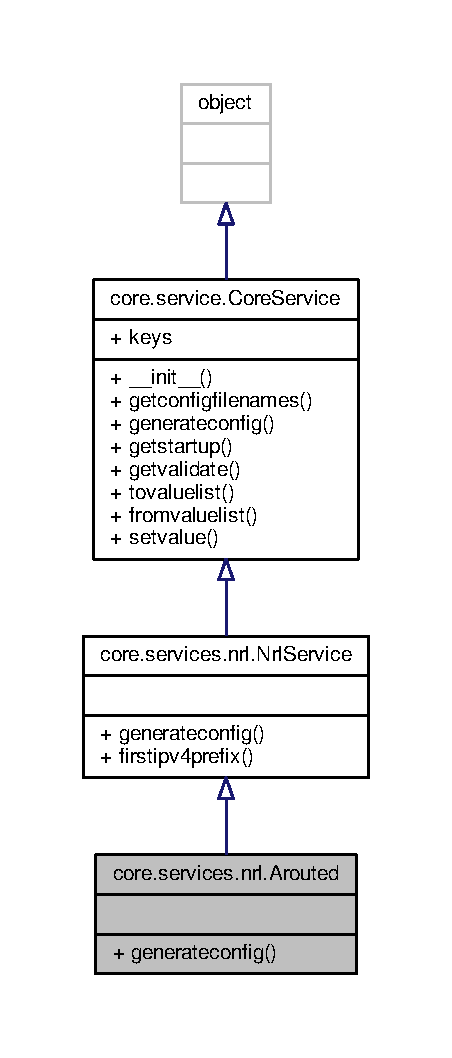
\includegraphics[width=217pt]{classcore_1_1services_1_1nrl_1_1_arouted__inherit__graph}
\end{center}
\end{figure}


Collaboration diagram for core.\+services.\+nrl.\+Arouted\+:
\nopagebreak
\begin{figure}[H]
\begin{center}
\leavevmode
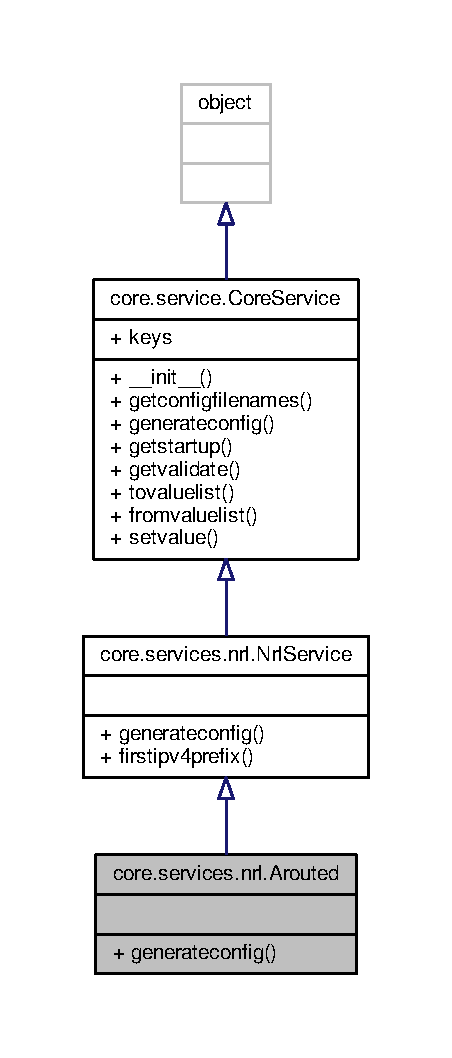
\includegraphics[width=217pt]{classcore_1_1services_1_1nrl_1_1_arouted__coll__graph}
\end{center}
\end{figure}
\subsection*{Public Member Functions}
\begin{DoxyCompactItemize}
\item 
def \hyperlink{classcore_1_1services_1_1nrl_1_1_arouted_a7f706c37edb10d2bb67e3e4cdd66210d}{generateconfig}
\end{DoxyCompactItemize}
\subsection*{Additional Inherited Members}


\subsection{Detailed Description}
\begin{DoxyVerb}Adaptive Routing
\end{DoxyVerb}
 

\subsection{Member Function Documentation}
\hypertarget{classcore_1_1services_1_1nrl_1_1_arouted_a7f706c37edb10d2bb67e3e4cdd66210d}{\index{core\+::services\+::nrl\+::\+Arouted@{core\+::services\+::nrl\+::\+Arouted}!generateconfig@{generateconfig}}
\index{generateconfig@{generateconfig}!core\+::services\+::nrl\+::\+Arouted@{core\+::services\+::nrl\+::\+Arouted}}
\subsubsection[{generateconfig}]{\setlength{\rightskip}{0pt plus 5cm}def core.\+services.\+nrl.\+Arouted.\+generateconfig (
\begin{DoxyParamCaption}
\item[{}]{cls, }
\item[{}]{node, }
\item[{}]{filename, }
\item[{}]{services}
\end{DoxyParamCaption}
)}}\label{classcore_1_1services_1_1nrl_1_1_arouted_a7f706c37edb10d2bb67e3e4cdd66210d}
\begin{DoxyVerb}Return the Quagga.conf or quaggaboot.sh file contents.
\end{DoxyVerb}
 

The documentation for this class was generated from the following file\+:\begin{DoxyCompactItemize}
\item 
daemon/core/services/nrl.\+py\end{DoxyCompactItemize}

\hypertarget{classcore_1_1services_1_1utility_1_1_atd_service}{\section{core.\+services.\+utility.\+Atd\+Service Class Reference}
\label{classcore_1_1services_1_1utility_1_1_atd_service}\index{core.\+services.\+utility.\+Atd\+Service@{core.\+services.\+utility.\+Atd\+Service}}
}


Inheritance diagram for core.\+services.\+utility.\+Atd\+Service\+:
\nopagebreak
\begin{figure}[H]
\begin{center}
\leavevmode
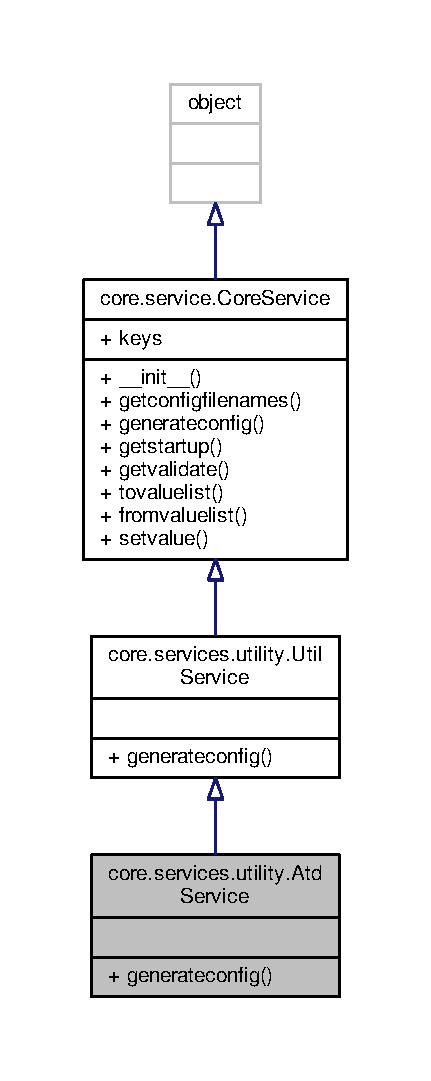
\includegraphics[width=207pt]{classcore_1_1services_1_1utility_1_1_atd_service__inherit__graph}
\end{center}
\end{figure}


Collaboration diagram for core.\+services.\+utility.\+Atd\+Service\+:
\nopagebreak
\begin{figure}[H]
\begin{center}
\leavevmode
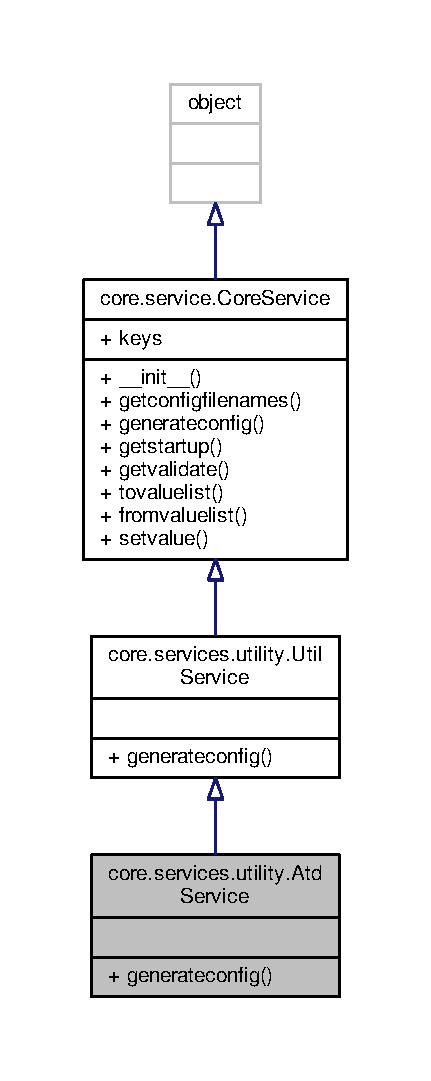
\includegraphics[width=207pt]{classcore_1_1services_1_1utility_1_1_atd_service__coll__graph}
\end{center}
\end{figure}
\subsection*{Public Member Functions}
\begin{DoxyCompactItemize}
\item 
\hypertarget{classcore_1_1services_1_1utility_1_1_atd_service_a1dd9144c6c48579fa865fb4667709fe9}{def {\bfseries generateconfig}}\label{classcore_1_1services_1_1utility_1_1_atd_service_a1dd9144c6c48579fa865fb4667709fe9}

\end{DoxyCompactItemize}
\subsection*{Additional Inherited Members}


\subsection{Detailed Description}
\begin{DoxyVerb}Atd service for scheduling at jobs
\end{DoxyVerb}
 

The documentation for this class was generated from the following file\+:\begin{DoxyCompactItemize}
\item 
daemon/core/services/utility.\+py\end{DoxyCompactItemize}

\hypertarget{classcore_1_1misc_1_1xmlwriter1_1_1_attrib}{\section{core.\+misc.\+xmlwriter1.\+Attrib Class Reference}
\label{classcore_1_1misc_1_1xmlwriter1_1_1_attrib}\index{core.\+misc.\+xmlwriter1.\+Attrib@{core.\+misc.\+xmlwriter1.\+Attrib}}
}


Inheritance diagram for core.\+misc.\+xmlwriter1.\+Attrib\+:
\nopagebreak
\begin{figure}[H]
\begin{center}
\leavevmode
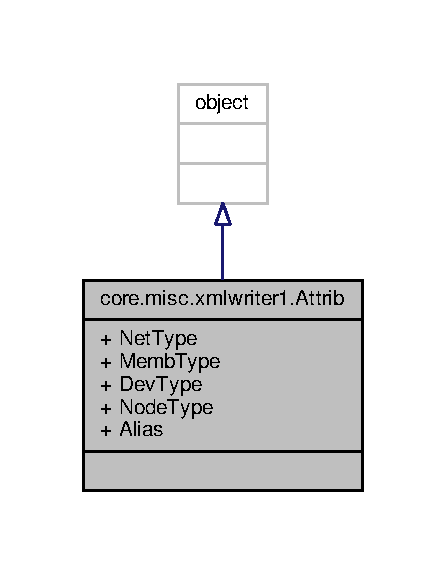
\includegraphics[width=214pt]{classcore_1_1misc_1_1xmlwriter1_1_1_attrib__inherit__graph}
\end{center}
\end{figure}


Collaboration diagram for core.\+misc.\+xmlwriter1.\+Attrib\+:
\nopagebreak
\begin{figure}[H]
\begin{center}
\leavevmode
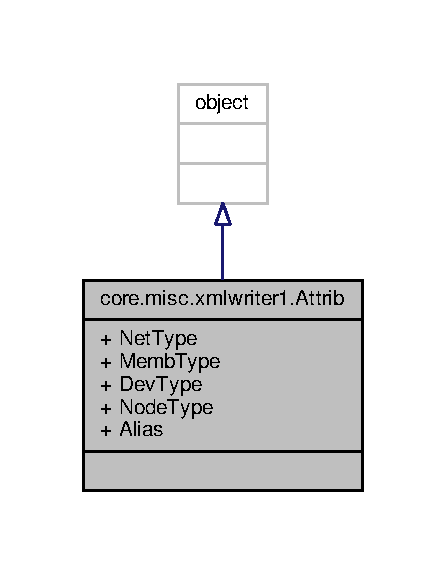
\includegraphics[width=214pt]{classcore_1_1misc_1_1xmlwriter1_1_1_attrib__coll__graph}
\end{center}
\end{figure}
\subsection*{Static Public Attributes}
\begin{DoxyCompactItemize}
\item 
tuple {\bfseries Net\+Type}
\item 
tuple {\bfseries Memb\+Type}
\item 
tuple {\bfseries Dev\+Type}
\item 
tuple {\bfseries Node\+Type}
\item 
\hypertarget{classcore_1_1misc_1_1xmlwriter1_1_1_attrib_a8796c33eb30cc243e726a66af21f2d77}{tuple {\bfseries Alias} = enum(I\+D = \char`\"{}C\+O\+R\+E\+I\+D\char`\"{})}\label{classcore_1_1misc_1_1xmlwriter1_1_1_attrib_a8796c33eb30cc243e726a66af21f2d77}

\end{DoxyCompactItemize}


\subsection{Detailed Description}
\begin{DoxyVerb}NMF scenario plan attribute constants
\end{DoxyVerb}
 

\subsection{Member Data Documentation}
\hypertarget{classcore_1_1misc_1_1xmlwriter1_1_1_attrib_af62b4beecf187fd42434df9d51f36920}{\index{core\+::misc\+::xmlwriter1\+::\+Attrib@{core\+::misc\+::xmlwriter1\+::\+Attrib}!Dev\+Type@{Dev\+Type}}
\index{Dev\+Type@{Dev\+Type}!core\+::misc\+::xmlwriter1\+::\+Attrib@{core\+::misc\+::xmlwriter1\+::\+Attrib}}
\subsubsection[{Dev\+Type}]{\setlength{\rightskip}{0pt plus 5cm}tuple core.\+misc.\+xmlwriter1.\+Attrib.\+Dev\+Type\hspace{0.3cm}{\ttfamily [static]}}}\label{classcore_1_1misc_1_1xmlwriter1_1_1_attrib_af62b4beecf187fd42434df9d51f36920}
{\bfseries Initial value\+:}
\begin{DoxyCode}
1 = enum(HOST = \textcolor{stringliteral}{'host'}, ROUTER = \textcolor{stringliteral}{'router'}, SWITCH = \textcolor{stringliteral}{'switch'},
2                    HUB = \textcolor{stringliteral}{'hub'})
\end{DoxyCode}
\hypertarget{classcore_1_1misc_1_1xmlwriter1_1_1_attrib_a2e5551433d9f8c7d4228113972d8d167}{\index{core\+::misc\+::xmlwriter1\+::\+Attrib@{core\+::misc\+::xmlwriter1\+::\+Attrib}!Memb\+Type@{Memb\+Type}}
\index{Memb\+Type@{Memb\+Type}!core\+::misc\+::xmlwriter1\+::\+Attrib@{core\+::misc\+::xmlwriter1\+::\+Attrib}}
\subsubsection[{Memb\+Type}]{\setlength{\rightskip}{0pt plus 5cm}tuple core.\+misc.\+xmlwriter1.\+Attrib.\+Memb\+Type\hspace{0.3cm}{\ttfamily [static]}}}\label{classcore_1_1misc_1_1xmlwriter1_1_1_attrib_a2e5551433d9f8c7d4228113972d8d167}
{\bfseries Initial value\+:}
\begin{DoxyCode}
1 = enum(INTERFACE = \textcolor{stringliteral}{'interface'}, CHANNEL = \textcolor{stringliteral}{'channel'},
2                     SWITCH = \textcolor{stringliteral}{'switch'}, HUB = \textcolor{stringliteral}{'hub'}, TUNNEL = \textcolor{stringliteral}{'tunnel'},
3                     NETWORK = \textcolor{stringliteral}{"network"})
\end{DoxyCode}
\hypertarget{classcore_1_1misc_1_1xmlwriter1_1_1_attrib_afee91d12eeccd3afbf4fcf3c3b2bbe25}{\index{core\+::misc\+::xmlwriter1\+::\+Attrib@{core\+::misc\+::xmlwriter1\+::\+Attrib}!Net\+Type@{Net\+Type}}
\index{Net\+Type@{Net\+Type}!core\+::misc\+::xmlwriter1\+::\+Attrib@{core\+::misc\+::xmlwriter1\+::\+Attrib}}
\subsubsection[{Net\+Type}]{\setlength{\rightskip}{0pt plus 5cm}tuple core.\+misc.\+xmlwriter1.\+Attrib.\+Net\+Type\hspace{0.3cm}{\ttfamily [static]}}}\label{classcore_1_1misc_1_1xmlwriter1_1_1_attrib_afee91d12eeccd3afbf4fcf3c3b2bbe25}
{\bfseries Initial value\+:}
\begin{DoxyCode}
1 = enum(WIRELESS = \textcolor{stringliteral}{'wireless'}, ETHERNET = \textcolor{stringliteral}{'ethernet'},
2                    PTP\_WIRED = \textcolor{stringliteral}{'point-to-point-wired'},
3                    PTP\_WIRELESS = \textcolor{stringliteral}{'point-to-point-wireless'})
\end{DoxyCode}
\hypertarget{classcore_1_1misc_1_1xmlwriter1_1_1_attrib_a994288366ffa4e207c881f9109155875}{\index{core\+::misc\+::xmlwriter1\+::\+Attrib@{core\+::misc\+::xmlwriter1\+::\+Attrib}!Node\+Type@{Node\+Type}}
\index{Node\+Type@{Node\+Type}!core\+::misc\+::xmlwriter1\+::\+Attrib@{core\+::misc\+::xmlwriter1\+::\+Attrib}}
\subsubsection[{Node\+Type}]{\setlength{\rightskip}{0pt plus 5cm}tuple core.\+misc.\+xmlwriter1.\+Attrib.\+Node\+Type\hspace{0.3cm}{\ttfamily [static]}}}\label{classcore_1_1misc_1_1xmlwriter1_1_1_attrib_a994288366ffa4e207c881f9109155875}
{\bfseries Initial value\+:}
\begin{DoxyCode}
1 = enum(ROUTER = \textcolor{stringliteral}{'router'}, HOST = \textcolor{stringliteral}{'host'}, MDR = \textcolor{stringliteral}{'mdr'},
2                     PC = \textcolor{stringliteral}{'PC'}, RJ45 = \textcolor{stringliteral}{'rj45'}, SWITCH = \textcolor{stringliteral}{'lanswitch'}, 
3                     HUB = \textcolor{stringliteral}{'hub'})
\end{DoxyCode}


The documentation for this class was generated from the following file\+:\begin{DoxyCompactItemize}
\item 
daemon/core/misc/xmlwriter1.\+py\end{DoxyCompactItemize}

\hypertarget{classcore_1_1services_1_1quagga_1_1_babel}{\section{core.\+services.\+quagga.\+Babel Class Reference}
\label{classcore_1_1services_1_1quagga_1_1_babel}\index{core.\+services.\+quagga.\+Babel@{core.\+services.\+quagga.\+Babel}}
}


Inheritance diagram for core.\+services.\+quagga.\+Babel\+:
\nopagebreak
\begin{figure}[H]
\begin{center}
\leavevmode
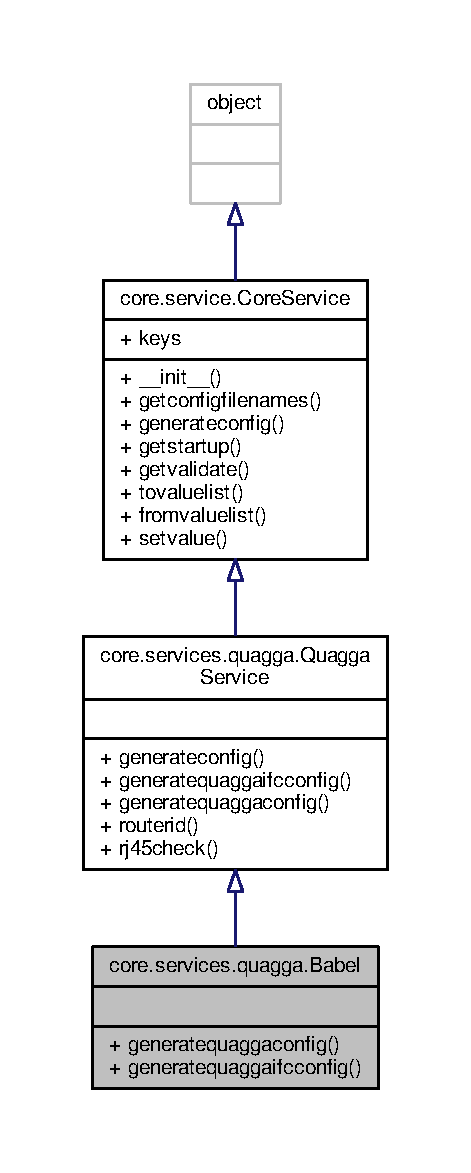
\includegraphics[height=550pt]{classcore_1_1services_1_1quagga_1_1_babel__inherit__graph}
\end{center}
\end{figure}


Collaboration diagram for core.\+services.\+quagga.\+Babel\+:
\nopagebreak
\begin{figure}[H]
\begin{center}
\leavevmode
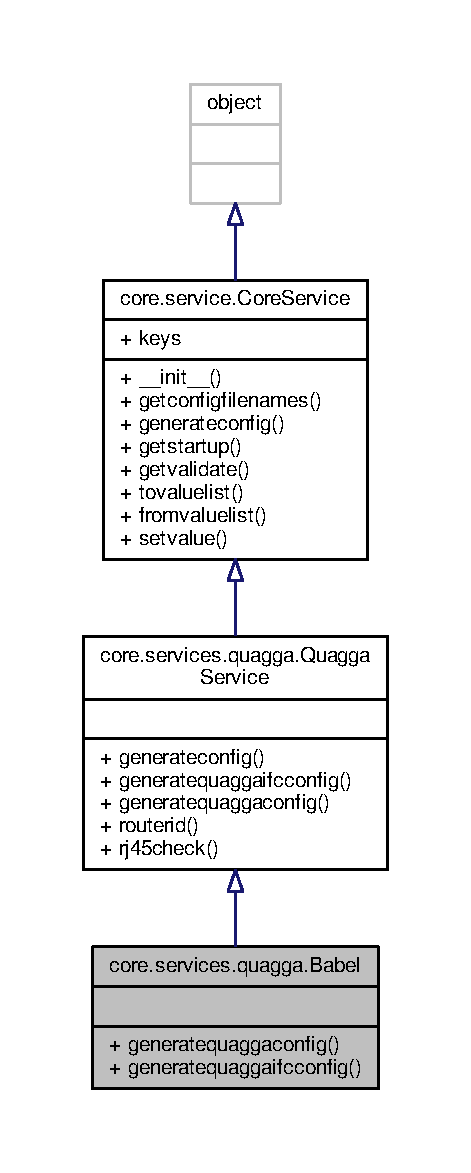
\includegraphics[height=550pt]{classcore_1_1services_1_1quagga_1_1_babel__coll__graph}
\end{center}
\end{figure}
\subsection*{Public Member Functions}
\begin{DoxyCompactItemize}
\item 
\hypertarget{classcore_1_1services_1_1quagga_1_1_babel_a4dfa901119b9efa705d7ffce367b3d53}{def {\bfseries generatequaggaconfig}}\label{classcore_1_1services_1_1quagga_1_1_babel_a4dfa901119b9efa705d7ffce367b3d53}

\item 
\hypertarget{classcore_1_1services_1_1quagga_1_1_babel_a5bc58a1afc3a64d1f674f4e926cd9a56}{def {\bfseries generatequaggaifcconfig}}\label{classcore_1_1services_1_1quagga_1_1_babel_a5bc58a1afc3a64d1f674f4e926cd9a56}

\end{DoxyCompactItemize}
\subsection*{Additional Inherited Members}


\subsection{Detailed Description}
\begin{DoxyVerb}The Babel service provides a loop-avoiding distance-vector routing 
protocol for IPv6 and IPv4 with fast convergence properties.
\end{DoxyVerb}
 

The documentation for this class was generated from the following file\+:\begin{DoxyCompactItemize}
\item 
daemon/core/services/quagga.\+py\end{DoxyCompactItemize}

\hypertarget{classcore_1_1coreserver_1_1_base_aux_request_handler}{\section{core.\+coreserver.\+Base\+Aux\+Request\+Handler Class Reference}
\label{classcore_1_1coreserver_1_1_base_aux_request_handler}\index{core.\+coreserver.\+Base\+Aux\+Request\+Handler@{core.\+coreserver.\+Base\+Aux\+Request\+Handler}}
}


Inheritance diagram for core.\+coreserver.\+Base\+Aux\+Request\+Handler\+:
\nopagebreak
\begin{figure}[H]
\begin{center}
\leavevmode
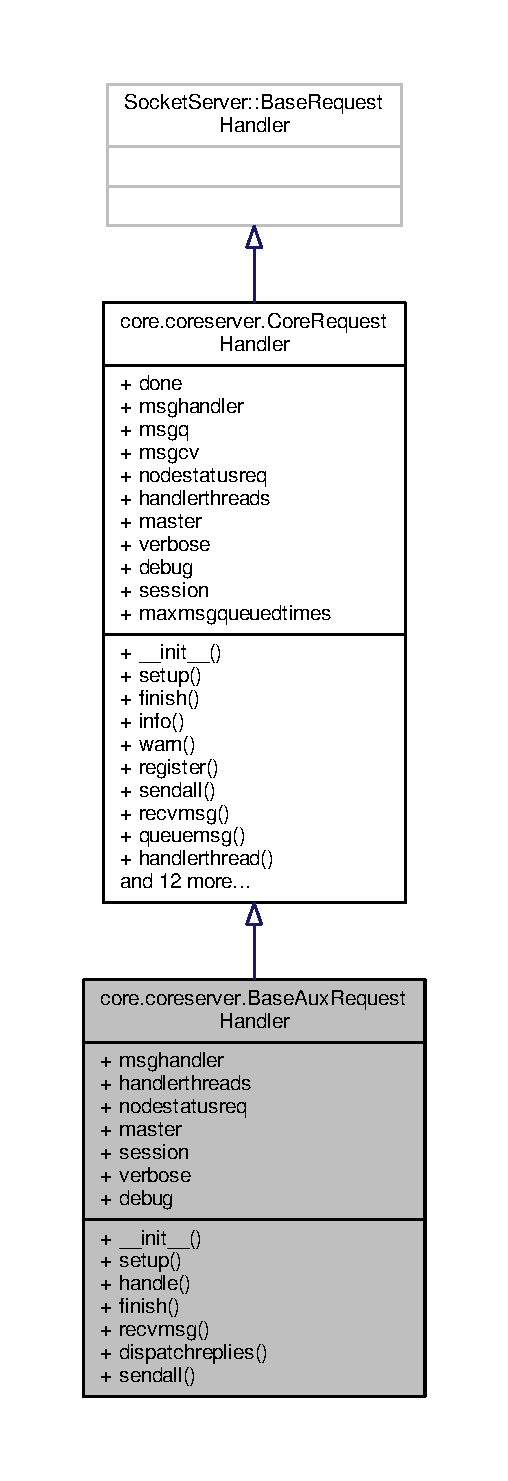
\includegraphics[height=550pt]{classcore_1_1coreserver_1_1_base_aux_request_handler__inherit__graph}
\end{center}
\end{figure}


Collaboration diagram for core.\+coreserver.\+Base\+Aux\+Request\+Handler\+:
\nopagebreak
\begin{figure}[H]
\begin{center}
\leavevmode
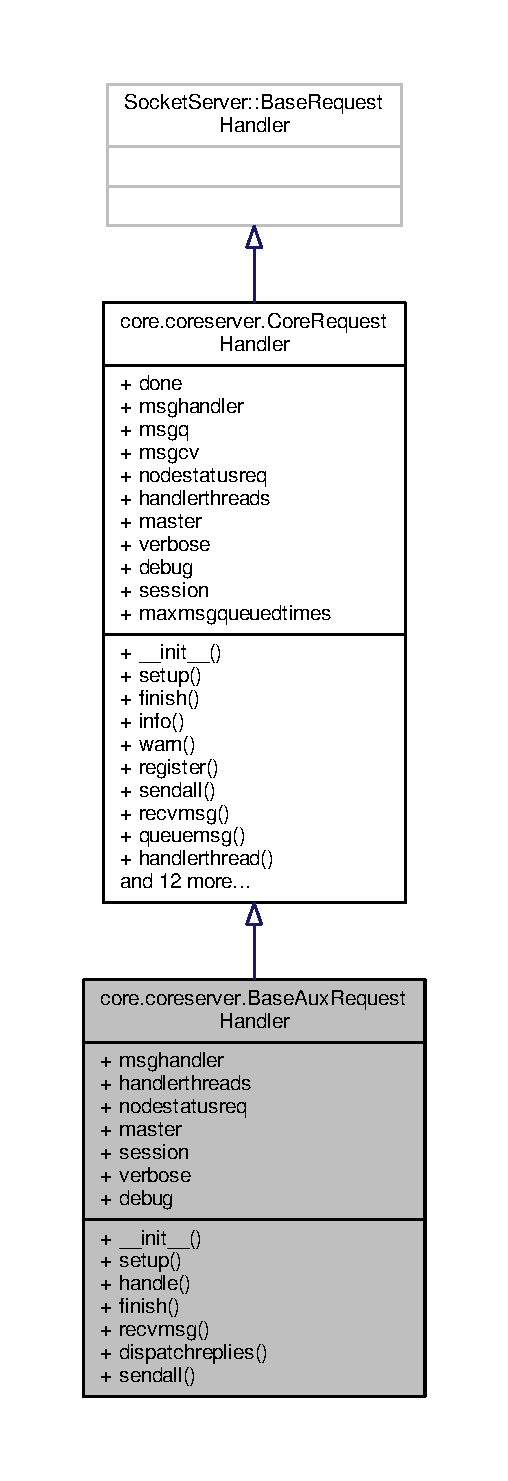
\includegraphics[height=550pt]{classcore_1_1coreserver_1_1_base_aux_request_handler__coll__graph}
\end{center}
\end{figure}
\subsection*{Public Member Functions}
\begin{DoxyCompactItemize}
\item 
\hypertarget{classcore_1_1coreserver_1_1_base_aux_request_handler_aa9e8b149d4f2e90604f006413d2ab60c}{def {\bfseries \+\_\+\+\_\+init\+\_\+\+\_\+}}\label{classcore_1_1coreserver_1_1_base_aux_request_handler_aa9e8b149d4f2e90604f006413d2ab60c}

\item 
def \hyperlink{classcore_1_1coreserver_1_1_base_aux_request_handler_a1d6c5553dcf495a800fa079a8658f114}{setup}
\item 
def \hyperlink{classcore_1_1coreserver_1_1_base_aux_request_handler_a3cdfb1427343be111d2eb899058b1815}{handle}
\item 
def \hyperlink{classcore_1_1coreserver_1_1_base_aux_request_handler_a7b8791e74aec916780321c8fe204d51d}{finish}
\item 
def \hyperlink{classcore_1_1coreserver_1_1_base_aux_request_handler_ab4ff99ecd6286d2e6e21993941020d4c}{recvmsg}
\item 
def \hyperlink{classcore_1_1coreserver_1_1_base_aux_request_handler_a630e62f71164ccc3a16edd4a0583f2a4}{dispatchreplies}
\item 
def \hyperlink{classcore_1_1coreserver_1_1_base_aux_request_handler_a2d8cfb919685bbc076a3737b0f0c14e7}{sendall}
\end{DoxyCompactItemize}
\subsection*{Public Attributes}
\begin{DoxyCompactItemize}
\item 
\hypertarget{classcore_1_1coreserver_1_1_base_aux_request_handler_a1dfec85bd6524a544048c5ab769b6a97}{{\bfseries msghandler}}\label{classcore_1_1coreserver_1_1_base_aux_request_handler_a1dfec85bd6524a544048c5ab769b6a97}

\item 
\hypertarget{classcore_1_1coreserver_1_1_base_aux_request_handler_a35e3510ca160b2d9d79609d74bf07a03}{{\bfseries handlerthreads}}\label{classcore_1_1coreserver_1_1_base_aux_request_handler_a35e3510ca160b2d9d79609d74bf07a03}

\item 
\hypertarget{classcore_1_1coreserver_1_1_base_aux_request_handler_aadb160941328111cc3af992c1238d2df}{{\bfseries nodestatusreq}}\label{classcore_1_1coreserver_1_1_base_aux_request_handler_aadb160941328111cc3af992c1238d2df}

\item 
\hypertarget{classcore_1_1coreserver_1_1_base_aux_request_handler_aadc370284a7b37032296cbbdca65888f}{{\bfseries master}}\label{classcore_1_1coreserver_1_1_base_aux_request_handler_aadc370284a7b37032296cbbdca65888f}

\item 
\hypertarget{classcore_1_1coreserver_1_1_base_aux_request_handler_a4b3e2889de14a30933dc0e18912ed65b}{{\bfseries session}}\label{classcore_1_1coreserver_1_1_base_aux_request_handler_a4b3e2889de14a30933dc0e18912ed65b}

\item 
\hypertarget{classcore_1_1coreserver_1_1_base_aux_request_handler_afd1d0dc58bc0dd476cbcef57f3cc71fd}{{\bfseries verbose}}\label{classcore_1_1coreserver_1_1_base_aux_request_handler_afd1d0dc58bc0dd476cbcef57f3cc71fd}

\item 
\hypertarget{classcore_1_1coreserver_1_1_base_aux_request_handler_a38338fa3388a26917348171d8248045b}{{\bfseries debug}}\label{classcore_1_1coreserver_1_1_base_aux_request_handler_a38338fa3388a26917348171d8248045b}

\end{DoxyCompactItemize}
\subsection*{Additional Inherited Members}


\subsection{Detailed Description}
\begin{DoxyVerb}This is the superclass for auxiliary handlers in CORE. A concrete auxiliary handler class
must, at a minimum, define the recvmsg(), sendall(), and dispatchreplies() methods.
See SockerServer.BaseRequestHandler for parameter details.
\end{DoxyVerb}
 

\subsection{Member Function Documentation}
\hypertarget{classcore_1_1coreserver_1_1_base_aux_request_handler_a630e62f71164ccc3a16edd4a0583f2a4}{\index{core\+::coreserver\+::\+Base\+Aux\+Request\+Handler@{core\+::coreserver\+::\+Base\+Aux\+Request\+Handler}!dispatchreplies@{dispatchreplies}}
\index{dispatchreplies@{dispatchreplies}!core\+::coreserver\+::\+Base\+Aux\+Request\+Handler@{core\+::coreserver\+::\+Base\+Aux\+Request\+Handler}}
\subsubsection[{dispatchreplies}]{\setlength{\rightskip}{0pt plus 5cm}def core.\+coreserver.\+Base\+Aux\+Request\+Handler.\+dispatchreplies (
\begin{DoxyParamCaption}
\item[{}]{self, }
\item[{}]{replies, }
\item[{}]{msg}
\end{DoxyParamCaption}
)}}\label{classcore_1_1coreserver_1_1_base_aux_request_handler_a630e62f71164ccc3a16edd4a0583f2a4}
\begin{DoxyVerb}Dispatch CORE 'replies' to a previously received message 'msg' from a client.
Replies passed to this method follow the CORE API. This method allows transformation to
the form supported by the auxiliary handler and within the context of 'msg'. 
Add transformation and transmission code here.

EXAMPLE:
transformed_replies = stateful_transform (replies, msg) # stateful_transform method needs to be defined
if transformed_replies:
    for reply in transformed_replies:
try:
    self.request.sendall(reply)
except Exception, e:
    if self.debug:
        self.info("-"*60)
        traceback.print_exc(file=sys.stdout)
        self.info("-"*60)
    raise e\end{DoxyVerb}
 \hypertarget{classcore_1_1coreserver_1_1_base_aux_request_handler_a7b8791e74aec916780321c8fe204d51d}{\index{core\+::coreserver\+::\+Base\+Aux\+Request\+Handler@{core\+::coreserver\+::\+Base\+Aux\+Request\+Handler}!finish@{finish}}
\index{finish@{finish}!core\+::coreserver\+::\+Base\+Aux\+Request\+Handler@{core\+::coreserver\+::\+Base\+Aux\+Request\+Handler}}
\subsubsection[{finish}]{\setlength{\rightskip}{0pt plus 5cm}def core.\+coreserver.\+Base\+Aux\+Request\+Handler.\+finish (
\begin{DoxyParamCaption}
\item[{}]{self}
\end{DoxyParamCaption}
)}}\label{classcore_1_1coreserver_1_1_base_aux_request_handler_a7b8791e74aec916780321c8fe204d51d}
\begin{DoxyVerb}Disconnect the client
\end{DoxyVerb}
 \hypertarget{classcore_1_1coreserver_1_1_base_aux_request_handler_a3cdfb1427343be111d2eb899058b1815}{\index{core\+::coreserver\+::\+Base\+Aux\+Request\+Handler@{core\+::coreserver\+::\+Base\+Aux\+Request\+Handler}!handle@{handle}}
\index{handle@{handle}!core\+::coreserver\+::\+Base\+Aux\+Request\+Handler@{core\+::coreserver\+::\+Base\+Aux\+Request\+Handler}}
\subsubsection[{handle}]{\setlength{\rightskip}{0pt plus 5cm}def core.\+coreserver.\+Base\+Aux\+Request\+Handler.\+handle (
\begin{DoxyParamCaption}
\item[{}]{self}
\end{DoxyParamCaption}
)}}\label{classcore_1_1coreserver_1_1_base_aux_request_handler_a3cdfb1427343be111d2eb899058b1815}
\begin{DoxyVerb}The handler main loop
\end{DoxyVerb}
 \hypertarget{classcore_1_1coreserver_1_1_base_aux_request_handler_ab4ff99ecd6286d2e6e21993941020d4c}{\index{core\+::coreserver\+::\+Base\+Aux\+Request\+Handler@{core\+::coreserver\+::\+Base\+Aux\+Request\+Handler}!recvmsg@{recvmsg}}
\index{recvmsg@{recvmsg}!core\+::coreserver\+::\+Base\+Aux\+Request\+Handler@{core\+::coreserver\+::\+Base\+Aux\+Request\+Handler}}
\subsubsection[{recvmsg}]{\setlength{\rightskip}{0pt plus 5cm}def core.\+coreserver.\+Base\+Aux\+Request\+Handler.\+recvmsg (
\begin{DoxyParamCaption}
\item[{}]{self}
\end{DoxyParamCaption}
)}}\label{classcore_1_1coreserver_1_1_base_aux_request_handler_ab4ff99ecd6286d2e6e21993941020d4c}
\begin{DoxyVerb}Receive data from the client in the supported format. Parse, transform to CORE API format and 
return transformed messages.

EXAMPLE:
return self.handler.request.recv(siz)\end{DoxyVerb}
 \hypertarget{classcore_1_1coreserver_1_1_base_aux_request_handler_a2d8cfb919685bbc076a3737b0f0c14e7}{\index{core\+::coreserver\+::\+Base\+Aux\+Request\+Handler@{core\+::coreserver\+::\+Base\+Aux\+Request\+Handler}!sendall@{sendall}}
\index{sendall@{sendall}!core\+::coreserver\+::\+Base\+Aux\+Request\+Handler@{core\+::coreserver\+::\+Base\+Aux\+Request\+Handler}}
\subsubsection[{sendall}]{\setlength{\rightskip}{0pt plus 5cm}def core.\+coreserver.\+Base\+Aux\+Request\+Handler.\+sendall (
\begin{DoxyParamCaption}
\item[{}]{self, }
\item[{}]{data}
\end{DoxyParamCaption}
)}}\label{classcore_1_1coreserver_1_1_base_aux_request_handler_a2d8cfb919685bbc076a3737b0f0c14e7}
\begin{DoxyVerb}CORE calls this method when data needs to be asynchronously sent to a client. The data is
in CORE API format. This method allows transformation to the required format supported by this
handler prior to transmission. 

EXAMPLE:
msgs = self.transform(data)  # transform method needs to be defined
if msgs:
    for msg in msgs:
try:
    self.request.sendall(reply)
except Exception, e:
    if self.debug:
        self.info("-"*60)
        traceback.print_exc(file=sys.stdout)
        self.info("-"*60)
    raise e
\end{DoxyVerb}
 \hypertarget{classcore_1_1coreserver_1_1_base_aux_request_handler_a1d6c5553dcf495a800fa079a8658f114}{\index{core\+::coreserver\+::\+Base\+Aux\+Request\+Handler@{core\+::coreserver\+::\+Base\+Aux\+Request\+Handler}!setup@{setup}}
\index{setup@{setup}!core\+::coreserver\+::\+Base\+Aux\+Request\+Handler@{core\+::coreserver\+::\+Base\+Aux\+Request\+Handler}}
\subsubsection[{setup}]{\setlength{\rightskip}{0pt plus 5cm}def core.\+coreserver.\+Base\+Aux\+Request\+Handler.\+setup (
\begin{DoxyParamCaption}
\item[{}]{self}
\end{DoxyParamCaption}
)}}\label{classcore_1_1coreserver_1_1_base_aux_request_handler_a1d6c5553dcf495a800fa079a8658f114}
\begin{DoxyVerb}New client has connected to the auxiliary server.
\end{DoxyVerb}
 

The documentation for this class was generated from the following file\+:\begin{DoxyCompactItemize}
\item 
daemon/core/coreserver.\+py\end{DoxyCompactItemize}

\hypertarget{classcore_1_1mobility_1_1_basic_range_model}{\section{core.\+mobility.\+Basic\+Range\+Model Class Reference}
\label{classcore_1_1mobility_1_1_basic_range_model}\index{core.\+mobility.\+Basic\+Range\+Model@{core.\+mobility.\+Basic\+Range\+Model}}
}


Inheritance diagram for core.\+mobility.\+Basic\+Range\+Model\+:
\nopagebreak
\begin{figure}[H]
\begin{center}
\leavevmode
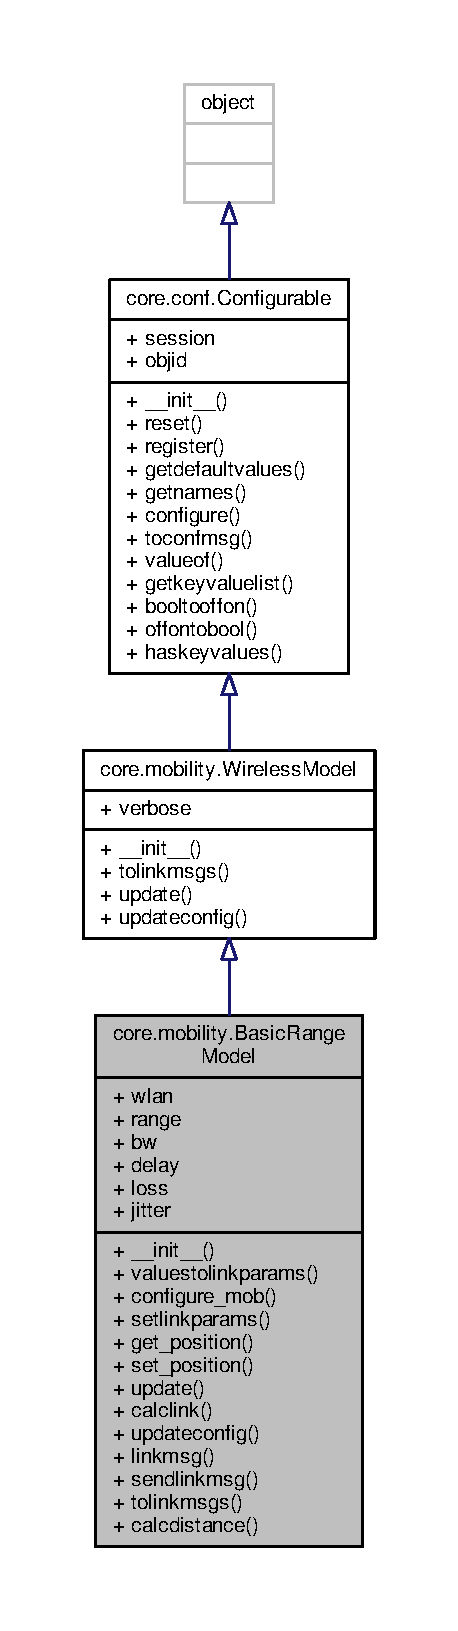
\includegraphics[height=550pt]{classcore_1_1mobility_1_1_basic_range_model__inherit__graph}
\end{center}
\end{figure}


Collaboration diagram for core.\+mobility.\+Basic\+Range\+Model\+:
\nopagebreak
\begin{figure}[H]
\begin{center}
\leavevmode
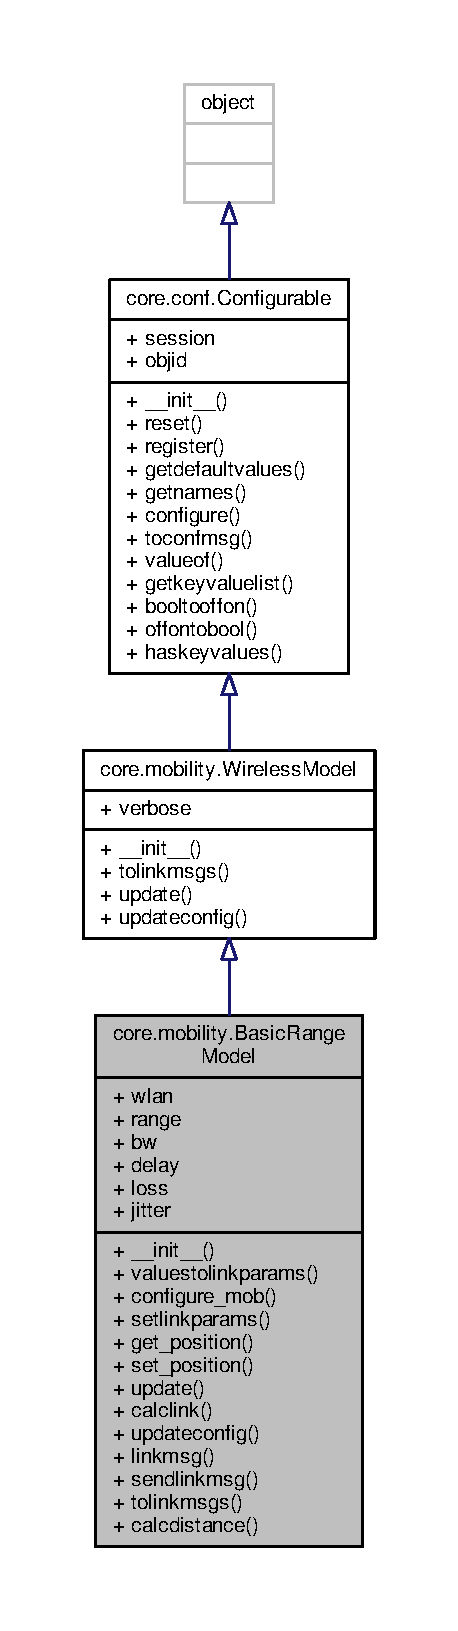
\includegraphics[height=550pt]{classcore_1_1mobility_1_1_basic_range_model__coll__graph}
\end{center}
\end{figure}
\subsection*{Public Member Functions}
\begin{DoxyCompactItemize}
\item 
def \hyperlink{classcore_1_1mobility_1_1_basic_range_model_a1b1a787ee56aeb4bb88996414e7d1022}{\+\_\+\+\_\+init\+\_\+\+\_\+}
\item 
\hypertarget{classcore_1_1mobility_1_1_basic_range_model_a80a50bece02da40abab69f1323697533}{def {\bfseries valuestolinkparams}}\label{classcore_1_1mobility_1_1_basic_range_model_a80a50bece02da40abab69f1323697533}

\item 
def \hyperlink{classcore_1_1mobility_1_1_basic_range_model_a47b1c565e5129fa98c288b4f8da887d7}{configure\+\_\+mob}
\item 
def \hyperlink{classcore_1_1mobility_1_1_basic_range_model_a7314252be7cef302ee6530a7e0759877}{setlinkparams}
\item 
\hypertarget{classcore_1_1mobility_1_1_basic_range_model_ae30a19d78b85b789050aee5152f7ae9e}{def {\bfseries get\+\_\+position}}\label{classcore_1_1mobility_1_1_basic_range_model_ae30a19d78b85b789050aee5152f7ae9e}

\item 
def \hyperlink{classcore_1_1mobility_1_1_basic_range_model_a8acc368e80977e4113473a91e4250524}{set\+\_\+position}
\item 
def \hyperlink{classcore_1_1mobility_1_1_basic_range_model_a1baebfc2ad0ebeb80cf3eb6b900e7d06}{update}
\item 
def \hyperlink{classcore_1_1mobility_1_1_basic_range_model_af5cb10ba600ceb6ed5828467f6219816}{calclink}
\item 
def \hyperlink{classcore_1_1mobility_1_1_basic_range_model_aef00a74c3391c0ff0639257328af3704}{updateconfig}
\item 
def \hyperlink{classcore_1_1mobility_1_1_basic_range_model_a40226f20b33f9a177e6d7ddbf4e1d02c}{linkmsg}
\item 
def \hyperlink{classcore_1_1mobility_1_1_basic_range_model_a1f632b74550bfc45684b63b9f1e74949}{sendlinkmsg}
\item 
def \hyperlink{classcore_1_1mobility_1_1_basic_range_model_a3f171e49d58eb03506ee54ce93e62b20}{tolinkmsgs}
\end{DoxyCompactItemize}
\subsection*{Static Public Member Functions}
\begin{DoxyCompactItemize}
\item 
def \hyperlink{classcore_1_1mobility_1_1_basic_range_model_aa8f655e22f439fafbfaf943536a39ba7}{calcdistance}
\end{DoxyCompactItemize}
\subsection*{Public Attributes}
\begin{DoxyCompactItemize}
\item 
\hypertarget{classcore_1_1mobility_1_1_basic_range_model_a2157d55e169d5810879c578e2eda6981}{{\bfseries wlan}}\label{classcore_1_1mobility_1_1_basic_range_model_a2157d55e169d5810879c578e2eda6981}

\item 
\hypertarget{classcore_1_1mobility_1_1_basic_range_model_a4784bd682091f43501b0631f0283d190}{{\bfseries range}}\label{classcore_1_1mobility_1_1_basic_range_model_a4784bd682091f43501b0631f0283d190}

\item 
\hypertarget{classcore_1_1mobility_1_1_basic_range_model_a51515ef835e37cf600ac57dd8934868c}{{\bfseries bw}}\label{classcore_1_1mobility_1_1_basic_range_model_a51515ef835e37cf600ac57dd8934868c}

\item 
\hypertarget{classcore_1_1mobility_1_1_basic_range_model_a1af42561ab9399d9cbb5dd6cdb5911a5}{{\bfseries delay}}\label{classcore_1_1mobility_1_1_basic_range_model_a1af42561ab9399d9cbb5dd6cdb5911a5}

\item 
\hypertarget{classcore_1_1mobility_1_1_basic_range_model_ac20c55cf1dcf544d769b657e3a8f826e}{{\bfseries loss}}\label{classcore_1_1mobility_1_1_basic_range_model_ac20c55cf1dcf544d769b657e3a8f826e}

\item 
\hypertarget{classcore_1_1mobility_1_1_basic_range_model_a7e6de2a415403d0183630a934fc2d0d1}{{\bfseries jitter}}\label{classcore_1_1mobility_1_1_basic_range_model_a7e6de2a415403d0183630a934fc2d0d1}

\end{DoxyCompactItemize}


\subsection{Detailed Description}
\begin{DoxyVerb}Basic Range wireless model, calculates range between nodes and links
and unlinks nodes based on this distance. This was formerly done from
the GUI.
\end{DoxyVerb}
 

\subsection{Constructor \& Destructor Documentation}
\hypertarget{classcore_1_1mobility_1_1_basic_range_model_a1b1a787ee56aeb4bb88996414e7d1022}{\index{core\+::mobility\+::\+Basic\+Range\+Model@{core\+::mobility\+::\+Basic\+Range\+Model}!\+\_\+\+\_\+init\+\_\+\+\_\+@{\+\_\+\+\_\+init\+\_\+\+\_\+}}
\index{\+\_\+\+\_\+init\+\_\+\+\_\+@{\+\_\+\+\_\+init\+\_\+\+\_\+}!core\+::mobility\+::\+Basic\+Range\+Model@{core\+::mobility\+::\+Basic\+Range\+Model}}
\subsubsection[{\+\_\+\+\_\+init\+\_\+\+\_\+}]{\setlength{\rightskip}{0pt plus 5cm}def core.\+mobility.\+Basic\+Range\+Model.\+\_\+\+\_\+init\+\_\+\+\_\+ (
\begin{DoxyParamCaption}
\item[{}]{self, }
\item[{}]{session, }
\item[{}]{objid, }
\item[{}]{verbose = {\ttfamily False}, }
\item[{}]{values = {\ttfamily None}}
\end{DoxyParamCaption}
)}}\label{classcore_1_1mobility_1_1_basic_range_model_a1b1a787ee56aeb4bb88996414e7d1022}
\begin{DoxyVerb}Range model is only instantiated during runtime.
\end{DoxyVerb}
 

\subsection{Member Function Documentation}
\hypertarget{classcore_1_1mobility_1_1_basic_range_model_aa8f655e22f439fafbfaf943536a39ba7}{\index{core\+::mobility\+::\+Basic\+Range\+Model@{core\+::mobility\+::\+Basic\+Range\+Model}!calcdistance@{calcdistance}}
\index{calcdistance@{calcdistance}!core\+::mobility\+::\+Basic\+Range\+Model@{core\+::mobility\+::\+Basic\+Range\+Model}}
\subsubsection[{calcdistance}]{\setlength{\rightskip}{0pt plus 5cm}def core.\+mobility.\+Basic\+Range\+Model.\+calcdistance (
\begin{DoxyParamCaption}
\item[{}]{p1, }
\item[{}]{p2}
\end{DoxyParamCaption}
)\hspace{0.3cm}{\ttfamily [static]}}}\label{classcore_1_1mobility_1_1_basic_range_model_aa8f655e22f439fafbfaf943536a39ba7}
\begin{DoxyVerb}Calculate the distance between two three-dimensional points.
\end{DoxyVerb}
 \hypertarget{classcore_1_1mobility_1_1_basic_range_model_af5cb10ba600ceb6ed5828467f6219816}{\index{core\+::mobility\+::\+Basic\+Range\+Model@{core\+::mobility\+::\+Basic\+Range\+Model}!calclink@{calclink}}
\index{calclink@{calclink}!core\+::mobility\+::\+Basic\+Range\+Model@{core\+::mobility\+::\+Basic\+Range\+Model}}
\subsubsection[{calclink}]{\setlength{\rightskip}{0pt plus 5cm}def core.\+mobility.\+Basic\+Range\+Model.\+calclink (
\begin{DoxyParamCaption}
\item[{}]{self, }
\item[{}]{netif, }
\item[{}]{netif2}
\end{DoxyParamCaption}
)}}\label{classcore_1_1mobility_1_1_basic_range_model_af5cb10ba600ceb6ed5828467f6219816}
\begin{DoxyVerb}Helper used by set_position() and update() to
    calculate distance between two interfaces and perform
    linking/unlinking. Sends link/unlink messages and updates the
    WlanNode's linked dict.
\end{DoxyVerb}
 \hypertarget{classcore_1_1mobility_1_1_basic_range_model_a47b1c565e5129fa98c288b4f8da887d7}{\index{core\+::mobility\+::\+Basic\+Range\+Model@{core\+::mobility\+::\+Basic\+Range\+Model}!configure\+\_\+mob@{configure\+\_\+mob}}
\index{configure\+\_\+mob@{configure\+\_\+mob}!core\+::mobility\+::\+Basic\+Range\+Model@{core\+::mobility\+::\+Basic\+Range\+Model}}
\subsubsection[{configure\+\_\+mob}]{\setlength{\rightskip}{0pt plus 5cm}def core.\+mobility.\+Basic\+Range\+Model.\+configure\+\_\+mob (
\begin{DoxyParamCaption}
\item[{}]{cls, }
\item[{}]{session, }
\item[{}]{msg}
\end{DoxyParamCaption}
)}}\label{classcore_1_1mobility_1_1_basic_range_model_a47b1c565e5129fa98c288b4f8da887d7}
\begin{DoxyVerb}Handle configuration messages for setting up a model.
Pass the MobilityManager object as the manager object.
\end{DoxyVerb}
 \hypertarget{classcore_1_1mobility_1_1_basic_range_model_a40226f20b33f9a177e6d7ddbf4e1d02c}{\index{core\+::mobility\+::\+Basic\+Range\+Model@{core\+::mobility\+::\+Basic\+Range\+Model}!linkmsg@{linkmsg}}
\index{linkmsg@{linkmsg}!core\+::mobility\+::\+Basic\+Range\+Model@{core\+::mobility\+::\+Basic\+Range\+Model}}
\subsubsection[{linkmsg}]{\setlength{\rightskip}{0pt plus 5cm}def core.\+mobility.\+Basic\+Range\+Model.\+linkmsg (
\begin{DoxyParamCaption}
\item[{}]{self, }
\item[{}]{netif, }
\item[{}]{netif2, }
\item[{}]{flags}
\end{DoxyParamCaption}
)}}\label{classcore_1_1mobility_1_1_basic_range_model_a40226f20b33f9a177e6d7ddbf4e1d02c}
\begin{DoxyVerb}Create a wireless link/unlink API message.
\end{DoxyVerb}
 \hypertarget{classcore_1_1mobility_1_1_basic_range_model_a1f632b74550bfc45684b63b9f1e74949}{\index{core\+::mobility\+::\+Basic\+Range\+Model@{core\+::mobility\+::\+Basic\+Range\+Model}!sendlinkmsg@{sendlinkmsg}}
\index{sendlinkmsg@{sendlinkmsg}!core\+::mobility\+::\+Basic\+Range\+Model@{core\+::mobility\+::\+Basic\+Range\+Model}}
\subsubsection[{sendlinkmsg}]{\setlength{\rightskip}{0pt plus 5cm}def core.\+mobility.\+Basic\+Range\+Model.\+sendlinkmsg (
\begin{DoxyParamCaption}
\item[{}]{self, }
\item[{}]{netif, }
\item[{}]{netif2, }
\item[{}]{unlink = {\ttfamily False}}
\end{DoxyParamCaption}
)}}\label{classcore_1_1mobility_1_1_basic_range_model_a1f632b74550bfc45684b63b9f1e74949}
\begin{DoxyVerb}Send a wireless link/unlink API message to the GUI.
\end{DoxyVerb}
 \hypertarget{classcore_1_1mobility_1_1_basic_range_model_a8acc368e80977e4113473a91e4250524}{\index{core\+::mobility\+::\+Basic\+Range\+Model@{core\+::mobility\+::\+Basic\+Range\+Model}!set\+\_\+position@{set\+\_\+position}}
\index{set\+\_\+position@{set\+\_\+position}!core\+::mobility\+::\+Basic\+Range\+Model@{core\+::mobility\+::\+Basic\+Range\+Model}}
\subsubsection[{set\+\_\+position}]{\setlength{\rightskip}{0pt plus 5cm}def core.\+mobility.\+Basic\+Range\+Model.\+set\+\_\+position (
\begin{DoxyParamCaption}
\item[{}]{self, }
\item[{}]{netif, }
\item[{}]{x = {\ttfamily None}, }
\item[{}]{y = {\ttfamily None}, }
\item[{}]{z = {\ttfamily None}}
\end{DoxyParamCaption}
)}}\label{classcore_1_1mobility_1_1_basic_range_model_a8acc368e80977e4113473a91e4250524}
\begin{DoxyVerb}A node has moved; given an interface, a new (x,y,z) position has
been set; calculate the new distance between other nodes and link or
unlink node pairs based on the configured range.
\end{DoxyVerb}
 \hypertarget{classcore_1_1mobility_1_1_basic_range_model_a7314252be7cef302ee6530a7e0759877}{\index{core\+::mobility\+::\+Basic\+Range\+Model@{core\+::mobility\+::\+Basic\+Range\+Model}!setlinkparams@{setlinkparams}}
\index{setlinkparams@{setlinkparams}!core\+::mobility\+::\+Basic\+Range\+Model@{core\+::mobility\+::\+Basic\+Range\+Model}}
\subsubsection[{setlinkparams}]{\setlength{\rightskip}{0pt plus 5cm}def core.\+mobility.\+Basic\+Range\+Model.\+setlinkparams (
\begin{DoxyParamCaption}
\item[{}]{self}
\end{DoxyParamCaption}
)}}\label{classcore_1_1mobility_1_1_basic_range_model_a7314252be7cef302ee6530a7e0759877}
\begin{DoxyVerb}Apply link parameters to all interfaces. This is invoked from
WlanNode.setmodel() after the position callback has been set.
\end{DoxyVerb}
 \hypertarget{classcore_1_1mobility_1_1_basic_range_model_a3f171e49d58eb03506ee54ce93e62b20}{\index{core\+::mobility\+::\+Basic\+Range\+Model@{core\+::mobility\+::\+Basic\+Range\+Model}!tolinkmsgs@{tolinkmsgs}}
\index{tolinkmsgs@{tolinkmsgs}!core\+::mobility\+::\+Basic\+Range\+Model@{core\+::mobility\+::\+Basic\+Range\+Model}}
\subsubsection[{tolinkmsgs}]{\setlength{\rightskip}{0pt plus 5cm}def core.\+mobility.\+Basic\+Range\+Model.\+tolinkmsgs (
\begin{DoxyParamCaption}
\item[{}]{self, }
\item[{}]{flags}
\end{DoxyParamCaption}
)}}\label{classcore_1_1mobility_1_1_basic_range_model_a3f171e49d58eb03506ee54ce93e62b20}
\begin{DoxyVerb}Return a list of wireless link messages for when the GUI reconnects.
\end{DoxyVerb}
 \hypertarget{classcore_1_1mobility_1_1_basic_range_model_a1baebfc2ad0ebeb80cf3eb6b900e7d06}{\index{core\+::mobility\+::\+Basic\+Range\+Model@{core\+::mobility\+::\+Basic\+Range\+Model}!update@{update}}
\index{update@{update}!core\+::mobility\+::\+Basic\+Range\+Model@{core\+::mobility\+::\+Basic\+Range\+Model}}
\subsubsection[{update}]{\setlength{\rightskip}{0pt plus 5cm}def core.\+mobility.\+Basic\+Range\+Model.\+update (
\begin{DoxyParamCaption}
\item[{}]{self, }
\item[{}]{moved, }
\item[{}]{moved\+\_\+netifs}
\end{DoxyParamCaption}
)}}\label{classcore_1_1mobility_1_1_basic_range_model_a1baebfc2ad0ebeb80cf3eb6b900e7d06}
\begin{DoxyVerb}Node positions have changed without recalc. Update positions from
node.position, then re-calculate links for those that have moved.
Assumes bidirectional links, with one calculation per node pair, where
one of the nodes has moved.
\end{DoxyVerb}
 \hypertarget{classcore_1_1mobility_1_1_basic_range_model_aef00a74c3391c0ff0639257328af3704}{\index{core\+::mobility\+::\+Basic\+Range\+Model@{core\+::mobility\+::\+Basic\+Range\+Model}!updateconfig@{updateconfig}}
\index{updateconfig@{updateconfig}!core\+::mobility\+::\+Basic\+Range\+Model@{core\+::mobility\+::\+Basic\+Range\+Model}}
\subsubsection[{updateconfig}]{\setlength{\rightskip}{0pt plus 5cm}def core.\+mobility.\+Basic\+Range\+Model.\+updateconfig (
\begin{DoxyParamCaption}
\item[{}]{self, }
\item[{}]{values}
\end{DoxyParamCaption}
)}}\label{classcore_1_1mobility_1_1_basic_range_model_aef00a74c3391c0ff0639257328af3704}
\begin{DoxyVerb}Configuration has changed during runtime.
MobilityManager.setconfig() -> WlanNode.updatemodel() -> 
WirelessModel.updateconfig()
\end{DoxyVerb}
 

The documentation for this class was generated from the following file\+:\begin{DoxyCompactItemize}
\item 
daemon/core/mobility.\+py\end{DoxyCompactItemize}

\hypertarget{classcore_1_1services_1_1quagga_1_1_bgp}{\section{core.\+services.\+quagga.\+Bgp Class Reference}
\label{classcore_1_1services_1_1quagga_1_1_bgp}\index{core.\+services.\+quagga.\+Bgp@{core.\+services.\+quagga.\+Bgp}}
}


Inheritance diagram for core.\+services.\+quagga.\+Bgp\+:
\nopagebreak
\begin{figure}[H]
\begin{center}
\leavevmode
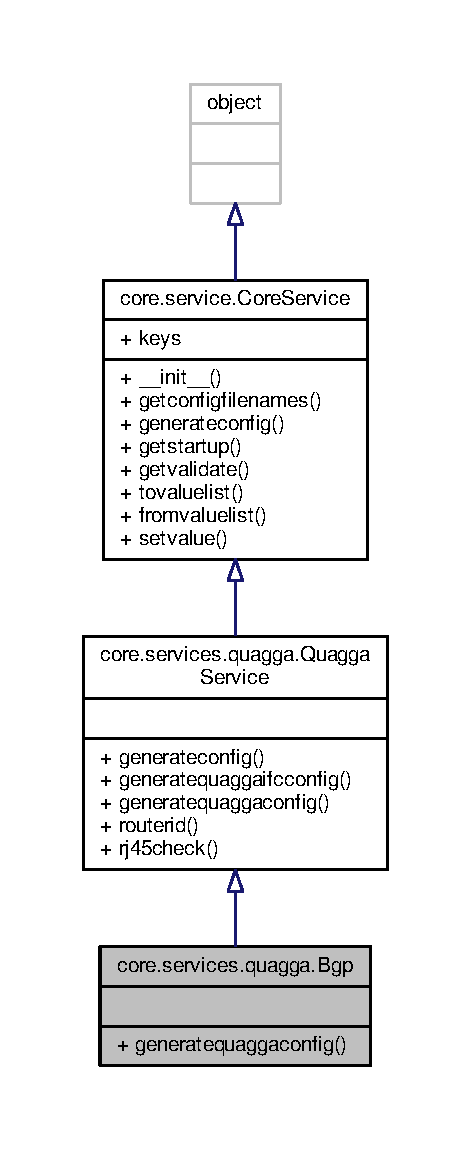
\includegraphics[height=550pt]{classcore_1_1services_1_1quagga_1_1_bgp__inherit__graph}
\end{center}
\end{figure}


Collaboration diagram for core.\+services.\+quagga.\+Bgp\+:
\nopagebreak
\begin{figure}[H]
\begin{center}
\leavevmode
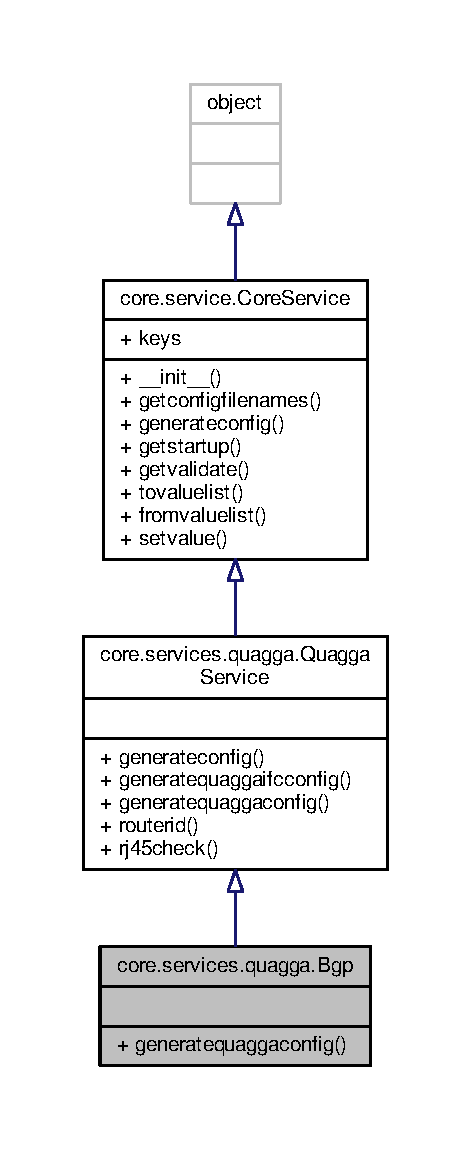
\includegraphics[height=550pt]{classcore_1_1services_1_1quagga_1_1_bgp__coll__graph}
\end{center}
\end{figure}
\subsection*{Public Member Functions}
\begin{DoxyCompactItemize}
\item 
\hypertarget{classcore_1_1services_1_1quagga_1_1_bgp_a2fe5e5d413ecf06a90dfc7bacca76af2}{def {\bfseries generatequaggaconfig}}\label{classcore_1_1services_1_1quagga_1_1_bgp_a2fe5e5d413ecf06a90dfc7bacca76af2}

\end{DoxyCompactItemize}
\subsection*{Additional Inherited Members}


\subsection{Detailed Description}
\begin{DoxyVerb}' The BGP service provides interdomain routing.
    Peers must be manually configured, with a full mesh for those
    having the same AS number.
\end{DoxyVerb}
 

The documentation for this class was generated from the following file\+:\begin{DoxyCompactItemize}
\item 
daemon/core/services/quagga.\+py\end{DoxyCompactItemize}

\hypertarget{classcore_1_1services_1_1bird_1_1_bird}{\section{core.\+services.\+bird.\+Bird Class Reference}
\label{classcore_1_1services_1_1bird_1_1_bird}\index{core.\+services.\+bird.\+Bird@{core.\+services.\+bird.\+Bird}}
}


Inheritance diagram for core.\+services.\+bird.\+Bird\+:
\nopagebreak
\begin{figure}[H]
\begin{center}
\leavevmode
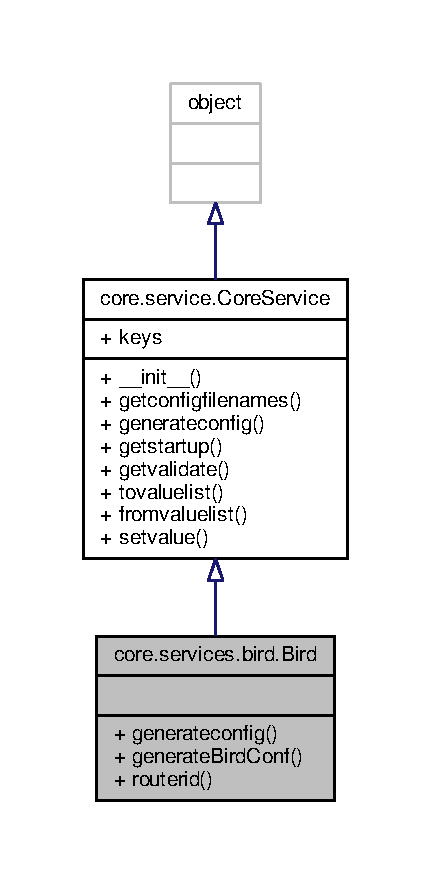
\includegraphics[width=207pt]{classcore_1_1services_1_1bird_1_1_bird__inherit__graph}
\end{center}
\end{figure}


Collaboration diagram for core.\+services.\+bird.\+Bird\+:
\nopagebreak
\begin{figure}[H]
\begin{center}
\leavevmode
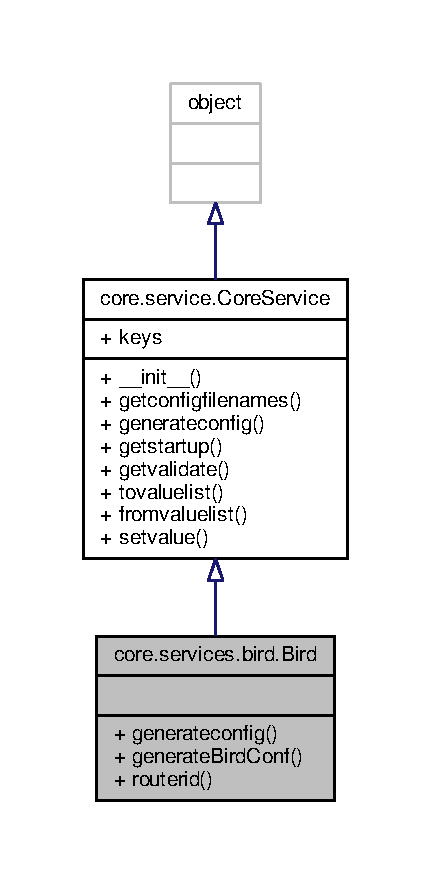
\includegraphics[width=207pt]{classcore_1_1services_1_1bird_1_1_bird__coll__graph}
\end{center}
\end{figure}
\subsection*{Public Member Functions}
\begin{DoxyCompactItemize}
\item 
def \hyperlink{classcore_1_1services_1_1bird_1_1_bird_a616b0a597c736f30a3e5e3428c8c214c}{generateconfig}
\item 
def \hyperlink{classcore_1_1services_1_1bird_1_1_bird_a3b3dcd09d93a0c55dc1402b0a8cd5c2f}{generate\+Bird\+Conf}
\end{DoxyCompactItemize}
\subsection*{Static Public Member Functions}
\begin{DoxyCompactItemize}
\item 
def \hyperlink{classcore_1_1services_1_1bird_1_1_bird_a7b79dbcd32714b3e99711bf4a7113328}{routerid}
\end{DoxyCompactItemize}
\subsection*{Additional Inherited Members}


\subsection{Detailed Description}
\begin{DoxyVerb}Bird router support
\end{DoxyVerb}
 

\subsection{Member Function Documentation}
\hypertarget{classcore_1_1services_1_1bird_1_1_bird_a3b3dcd09d93a0c55dc1402b0a8cd5c2f}{\index{core\+::services\+::bird\+::\+Bird@{core\+::services\+::bird\+::\+Bird}!generate\+Bird\+Conf@{generate\+Bird\+Conf}}
\index{generate\+Bird\+Conf@{generate\+Bird\+Conf}!core\+::services\+::bird\+::\+Bird@{core\+::services\+::bird\+::\+Bird}}
\subsubsection[{generate\+Bird\+Conf}]{\setlength{\rightskip}{0pt plus 5cm}def core.\+services.\+bird.\+Bird.\+generate\+Bird\+Conf (
\begin{DoxyParamCaption}
\item[{}]{cls, }
\item[{}]{node, }
\item[{}]{services}
\end{DoxyParamCaption}
)}}\label{classcore_1_1services_1_1bird_1_1_bird_a3b3dcd09d93a0c55dc1402b0a8cd5c2f}
\begin{DoxyVerb}Returns configuration file text. Other services that depend on bird
   will have generatebirdifcconfig() and generatebirdconfig()
   hooks that are invoked here.
\end{DoxyVerb}
 \hypertarget{classcore_1_1services_1_1bird_1_1_bird_a616b0a597c736f30a3e5e3428c8c214c}{\index{core\+::services\+::bird\+::\+Bird@{core\+::services\+::bird\+::\+Bird}!generateconfig@{generateconfig}}
\index{generateconfig@{generateconfig}!core\+::services\+::bird\+::\+Bird@{core\+::services\+::bird\+::\+Bird}}
\subsubsection[{generateconfig}]{\setlength{\rightskip}{0pt plus 5cm}def core.\+services.\+bird.\+Bird.\+generateconfig (
\begin{DoxyParamCaption}
\item[{}]{cls, }
\item[{}]{node, }
\item[{}]{filename, }
\item[{}]{services}
\end{DoxyParamCaption}
)}}\label{classcore_1_1services_1_1bird_1_1_bird_a616b0a597c736f30a3e5e3428c8c214c}
\begin{DoxyVerb}Return the bird.conf file contents.
\end{DoxyVerb}
 \hypertarget{classcore_1_1services_1_1bird_1_1_bird_a7b79dbcd32714b3e99711bf4a7113328}{\index{core\+::services\+::bird\+::\+Bird@{core\+::services\+::bird\+::\+Bird}!routerid@{routerid}}
\index{routerid@{routerid}!core\+::services\+::bird\+::\+Bird@{core\+::services\+::bird\+::\+Bird}}
\subsubsection[{routerid}]{\setlength{\rightskip}{0pt plus 5cm}def core.\+services.\+bird.\+Bird.\+routerid (
\begin{DoxyParamCaption}
\item[{}]{node}
\end{DoxyParamCaption}
)\hspace{0.3cm}{\ttfamily [static]}}}\label{classcore_1_1services_1_1bird_1_1_bird_a7b79dbcd32714b3e99711bf4a7113328}
\begin{DoxyVerb}Helper to return the first IPv4 address of a node as its router ID.
\end{DoxyVerb}
 

The documentation for this class was generated from the following file\+:\begin{DoxyCompactItemize}
\item 
daemon/core/services/bird.\+py\end{DoxyCompactItemize}

\hypertarget{classcore_1_1services_1_1bird_1_1_bird_bgp}{\section{core.\+services.\+bird.\+Bird\+Bgp Class Reference}
\label{classcore_1_1services_1_1bird_1_1_bird_bgp}\index{core.\+services.\+bird.\+Bird\+Bgp@{core.\+services.\+bird.\+Bird\+Bgp}}
}


Inheritance diagram for core.\+services.\+bird.\+Bird\+Bgp\+:
\nopagebreak
\begin{figure}[H]
\begin{center}
\leavevmode
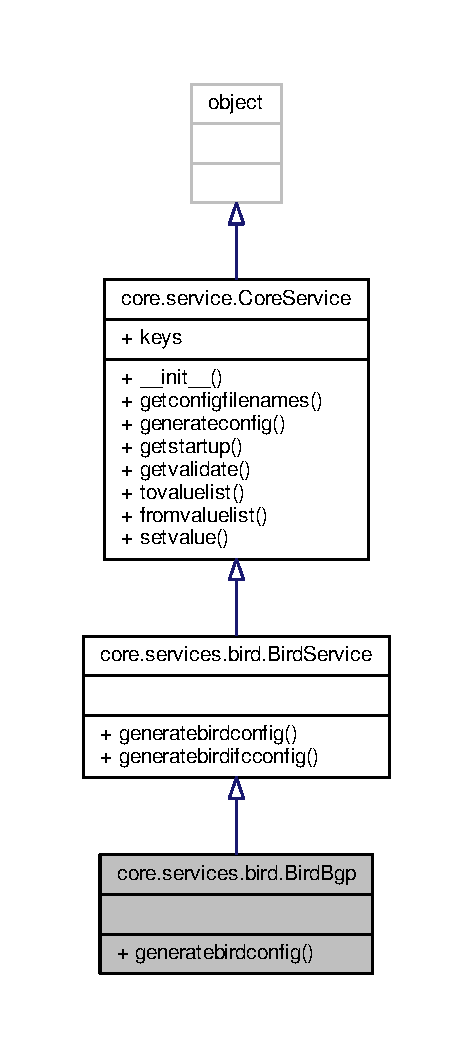
\includegraphics[width=227pt]{classcore_1_1services_1_1bird_1_1_bird_bgp__inherit__graph}
\end{center}
\end{figure}


Collaboration diagram for core.\+services.\+bird.\+Bird\+Bgp\+:
\nopagebreak
\begin{figure}[H]
\begin{center}
\leavevmode
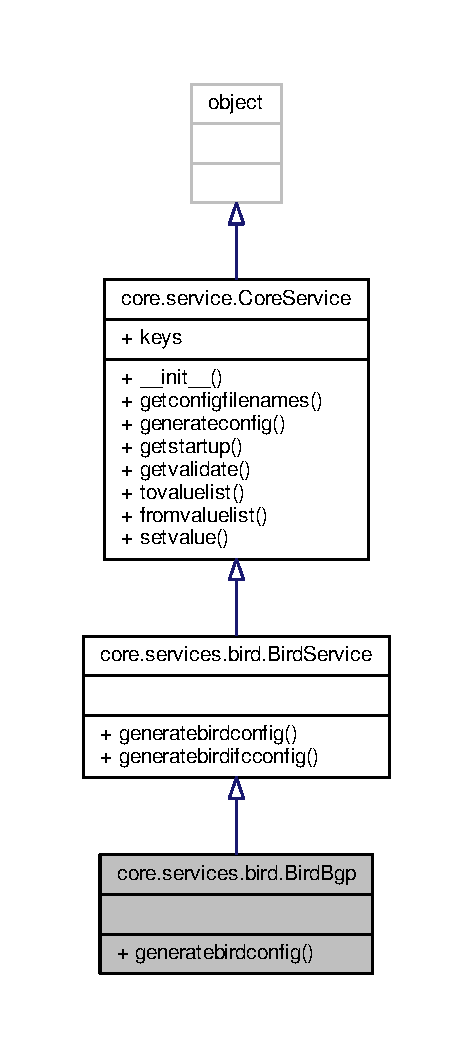
\includegraphics[width=227pt]{classcore_1_1services_1_1bird_1_1_bird_bgp__coll__graph}
\end{center}
\end{figure}
\subsection*{Public Member Functions}
\begin{DoxyCompactItemize}
\item 
\hypertarget{classcore_1_1services_1_1bird_1_1_bird_bgp_ae3c09051f02890eb985557f579d5ac32}{def {\bfseries generatebirdconfig}}\label{classcore_1_1services_1_1bird_1_1_bird_bgp_ae3c09051f02890eb985557f579d5ac32}

\end{DoxyCompactItemize}
\subsection*{Additional Inherited Members}


\subsection{Detailed Description}
\begin{DoxyVerb}BGP BIRD Service (configuration generation)\end{DoxyVerb}
 

The documentation for this class was generated from the following file\+:\begin{DoxyCompactItemize}
\item 
daemon/core/services/bird.\+py\end{DoxyCompactItemize}

\hypertarget{classcore_1_1services_1_1bird_1_1_bird_ospf}{\section{core.\+services.\+bird.\+Bird\+Ospf Class Reference}
\label{classcore_1_1services_1_1bird_1_1_bird_ospf}\index{core.\+services.\+bird.\+Bird\+Ospf@{core.\+services.\+bird.\+Bird\+Ospf}}
}


Inheritance diagram for core.\+services.\+bird.\+Bird\+Ospf\+:
\nopagebreak
\begin{figure}[H]
\begin{center}
\leavevmode
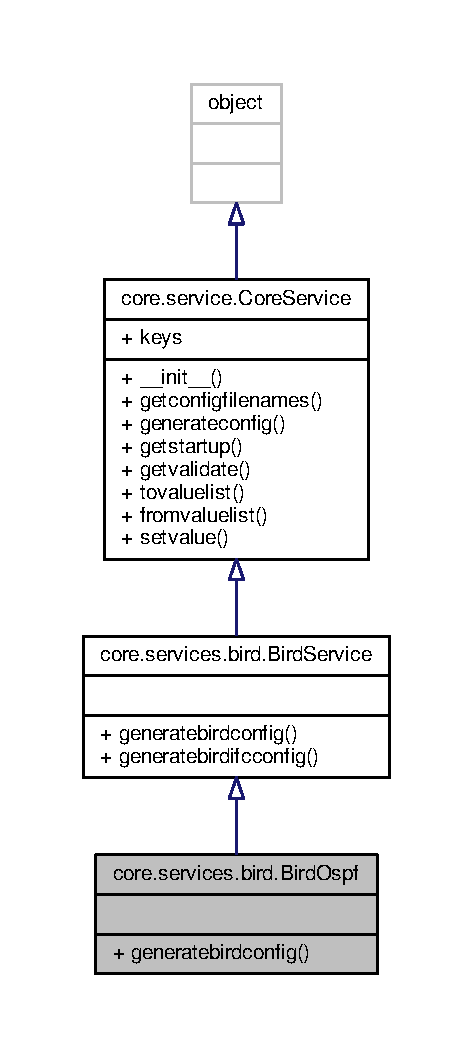
\includegraphics[width=227pt]{classcore_1_1services_1_1bird_1_1_bird_ospf__inherit__graph}
\end{center}
\end{figure}


Collaboration diagram for core.\+services.\+bird.\+Bird\+Ospf\+:
\nopagebreak
\begin{figure}[H]
\begin{center}
\leavevmode
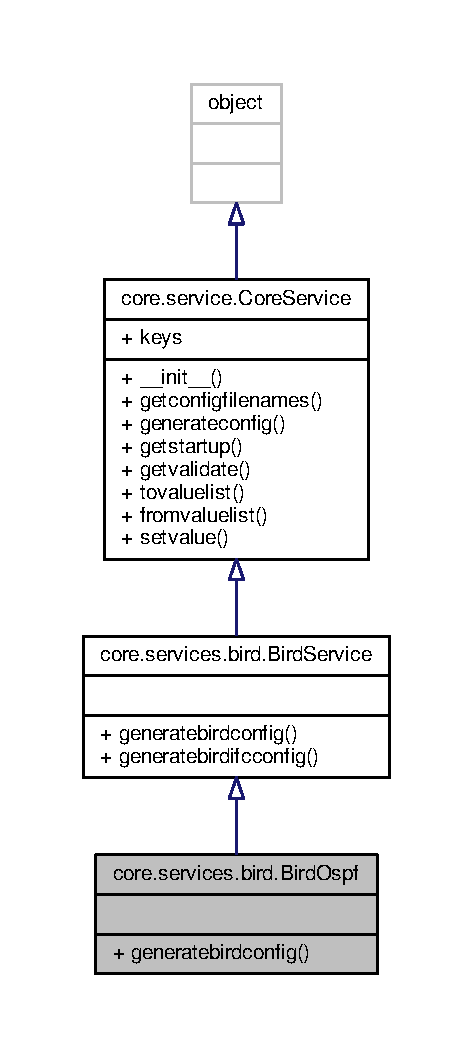
\includegraphics[width=227pt]{classcore_1_1services_1_1bird_1_1_bird_ospf__coll__graph}
\end{center}
\end{figure}
\subsection*{Public Member Functions}
\begin{DoxyCompactItemize}
\item 
\hypertarget{classcore_1_1services_1_1bird_1_1_bird_ospf_acfa6dd58ebf125bfbf337c83a4b603d8}{def {\bfseries generatebirdconfig}}\label{classcore_1_1services_1_1bird_1_1_bird_ospf_acfa6dd58ebf125bfbf337c83a4b603d8}

\end{DoxyCompactItemize}
\subsection*{Additional Inherited Members}


\subsection{Detailed Description}
\begin{DoxyVerb}OSPF BIRD Service (configuration generation)\end{DoxyVerb}
 

The documentation for this class was generated from the following file\+:\begin{DoxyCompactItemize}
\item 
daemon/core/services/bird.\+py\end{DoxyCompactItemize}

\hypertarget{classcore_1_1services_1_1bird_1_1_bird_radv}{\section{core.\+services.\+bird.\+Bird\+Radv Class Reference}
\label{classcore_1_1services_1_1bird_1_1_bird_radv}\index{core.\+services.\+bird.\+Bird\+Radv@{core.\+services.\+bird.\+Bird\+Radv}}
}


Inheritance diagram for core.\+services.\+bird.\+Bird\+Radv\+:
\nopagebreak
\begin{figure}[H]
\begin{center}
\leavevmode
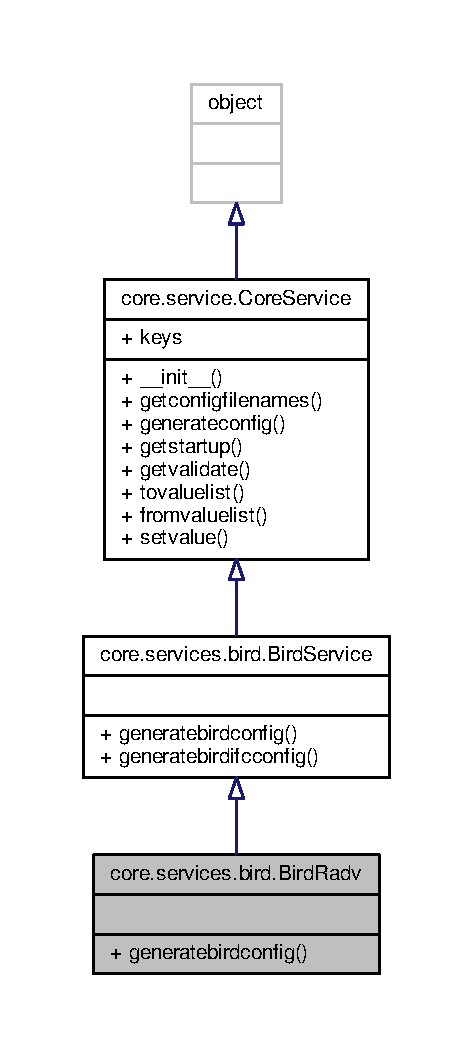
\includegraphics[width=227pt]{classcore_1_1services_1_1bird_1_1_bird_radv__inherit__graph}
\end{center}
\end{figure}


Collaboration diagram for core.\+services.\+bird.\+Bird\+Radv\+:
\nopagebreak
\begin{figure}[H]
\begin{center}
\leavevmode
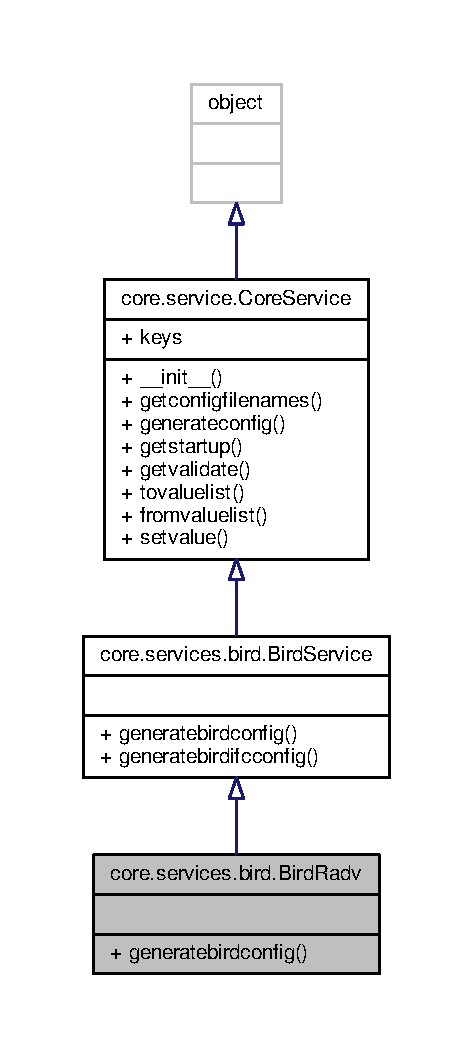
\includegraphics[width=227pt]{classcore_1_1services_1_1bird_1_1_bird_radv__coll__graph}
\end{center}
\end{figure}
\subsection*{Public Member Functions}
\begin{DoxyCompactItemize}
\item 
\hypertarget{classcore_1_1services_1_1bird_1_1_bird_radv_ac1f5e54cf7ed1ba83eb9fa0dea01624b}{def {\bfseries generatebirdconfig}}\label{classcore_1_1services_1_1bird_1_1_bird_radv_ac1f5e54cf7ed1ba83eb9fa0dea01624b}

\end{DoxyCompactItemize}
\subsection*{Additional Inherited Members}


\subsection{Detailed Description}
\begin{DoxyVerb}RADV BIRD Service (configuration generation)\end{DoxyVerb}
 

The documentation for this class was generated from the following file\+:\begin{DoxyCompactItemize}
\item 
daemon/core/services/bird.\+py\end{DoxyCompactItemize}

\hypertarget{classcore_1_1services_1_1bird_1_1_bird_rip}{\section{core.\+services.\+bird.\+Bird\+Rip Class Reference}
\label{classcore_1_1services_1_1bird_1_1_bird_rip}\index{core.\+services.\+bird.\+Bird\+Rip@{core.\+services.\+bird.\+Bird\+Rip}}
}


Inheritance diagram for core.\+services.\+bird.\+Bird\+Rip\+:
\nopagebreak
\begin{figure}[H]
\begin{center}
\leavevmode
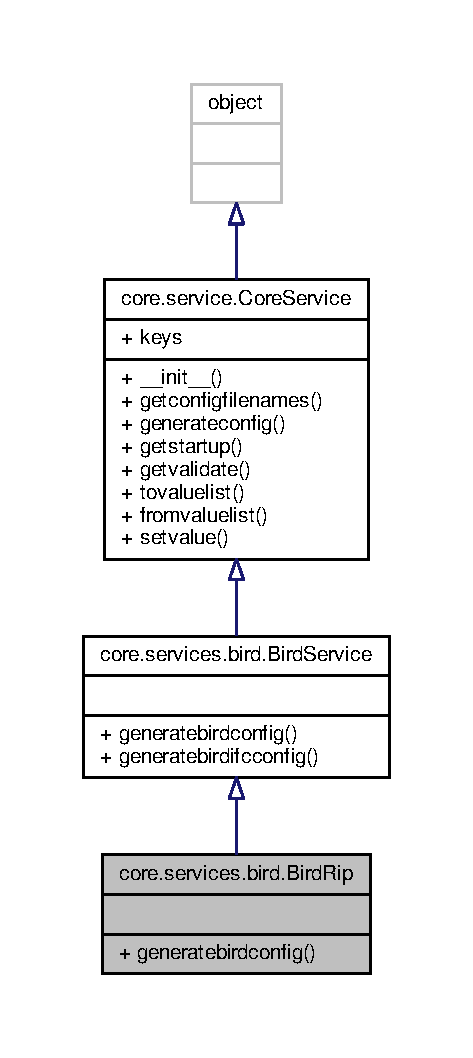
\includegraphics[width=227pt]{classcore_1_1services_1_1bird_1_1_bird_rip__inherit__graph}
\end{center}
\end{figure}


Collaboration diagram for core.\+services.\+bird.\+Bird\+Rip\+:
\nopagebreak
\begin{figure}[H]
\begin{center}
\leavevmode
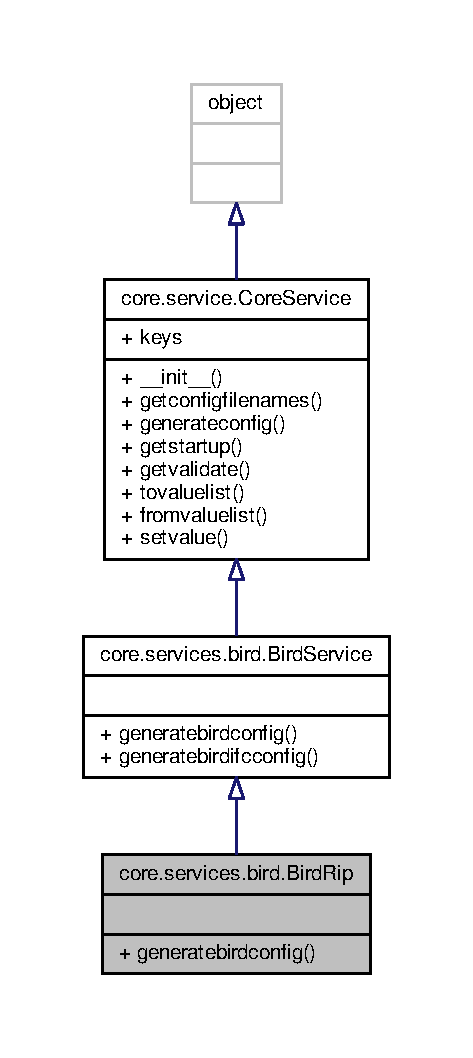
\includegraphics[width=227pt]{classcore_1_1services_1_1bird_1_1_bird_rip__coll__graph}
\end{center}
\end{figure}
\subsection*{Public Member Functions}
\begin{DoxyCompactItemize}
\item 
\hypertarget{classcore_1_1services_1_1bird_1_1_bird_rip_a46c425eaf1c563cf0ee7f8e28b140f67}{def {\bfseries generatebirdconfig}}\label{classcore_1_1services_1_1bird_1_1_bird_rip_a46c425eaf1c563cf0ee7f8e28b140f67}

\end{DoxyCompactItemize}
\subsection*{Additional Inherited Members}


\subsection{Detailed Description}
\begin{DoxyVerb}RIP BIRD Service (configuration generation)\end{DoxyVerb}
 

The documentation for this class was generated from the following file\+:\begin{DoxyCompactItemize}
\item 
daemon/core/services/bird.\+py\end{DoxyCompactItemize}

\hypertarget{classcore_1_1services_1_1bird_1_1_bird_service}{\section{core.\+services.\+bird.\+Bird\+Service Class Reference}
\label{classcore_1_1services_1_1bird_1_1_bird_service}\index{core.\+services.\+bird.\+Bird\+Service@{core.\+services.\+bird.\+Bird\+Service}}
}


Inheritance diagram for core.\+services.\+bird.\+Bird\+Service\+:
\nopagebreak
\begin{figure}[H]
\begin{center}
\leavevmode
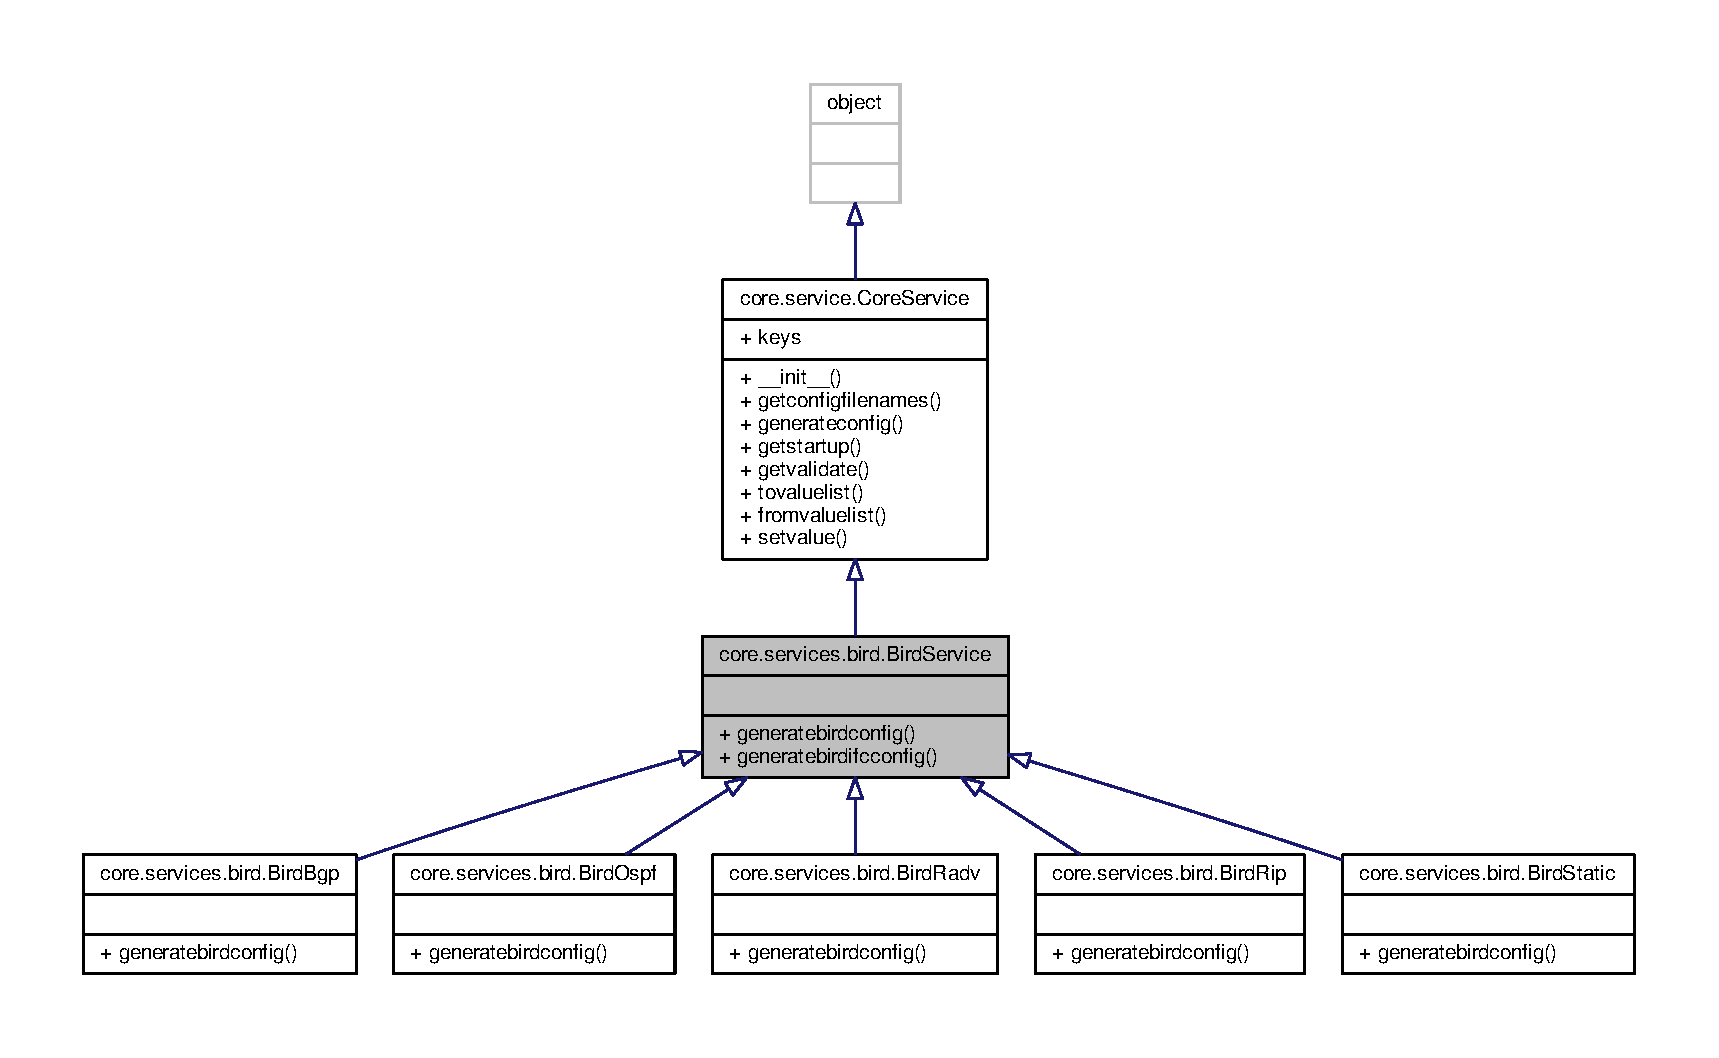
\includegraphics[width=350pt]{classcore_1_1services_1_1bird_1_1_bird_service__inherit__graph}
\end{center}
\end{figure}


Collaboration diagram for core.\+services.\+bird.\+Bird\+Service\+:
\nopagebreak
\begin{figure}[H]
\begin{center}
\leavevmode
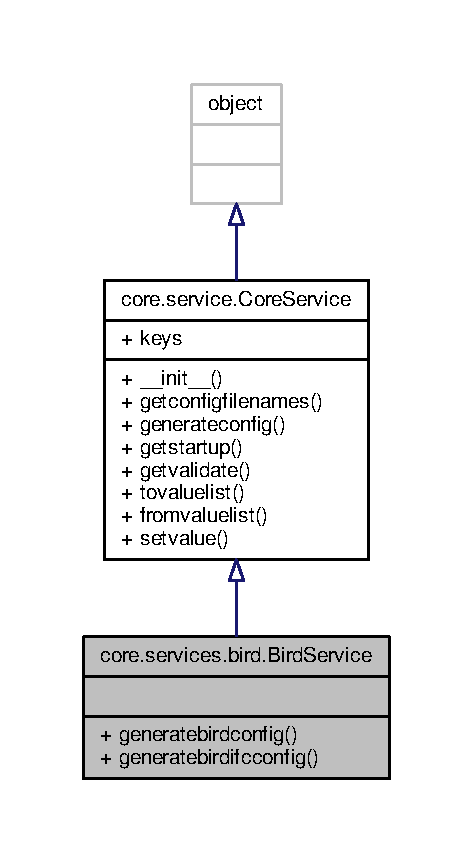
\includegraphics[width=227pt]{classcore_1_1services_1_1bird_1_1_bird_service__coll__graph}
\end{center}
\end{figure}
\subsection*{Public Member Functions}
\begin{DoxyCompactItemize}
\item 
\hypertarget{classcore_1_1services_1_1bird_1_1_bird_service_a24695f4ca2b67d0ad84201cd9447489e}{def {\bfseries generatebirdconfig}}\label{classcore_1_1services_1_1bird_1_1_bird_service_a24695f4ca2b67d0ad84201cd9447489e}

\item 
def \hyperlink{classcore_1_1services_1_1bird_1_1_bird_service_a01ffc743a85651342a3bcb2ad356fcf1}{generatebirdifcconfig}
\end{DoxyCompactItemize}
\subsection*{Additional Inherited Members}


\subsection{Detailed Description}
\begin{DoxyVerb}Parent class for Bird services. Defines properties and methods
common to Bird's routing daemons.
\end{DoxyVerb}
 

\subsection{Member Function Documentation}
\hypertarget{classcore_1_1services_1_1bird_1_1_bird_service_a01ffc743a85651342a3bcb2ad356fcf1}{\index{core\+::services\+::bird\+::\+Bird\+Service@{core\+::services\+::bird\+::\+Bird\+Service}!generatebirdifcconfig@{generatebirdifcconfig}}
\index{generatebirdifcconfig@{generatebirdifcconfig}!core\+::services\+::bird\+::\+Bird\+Service@{core\+::services\+::bird\+::\+Bird\+Service}}
\subsubsection[{generatebirdifcconfig}]{\setlength{\rightskip}{0pt plus 5cm}def core.\+services.\+bird.\+Bird\+Service.\+generatebirdifcconfig (
\begin{DoxyParamCaption}
\item[{}]{cls, }
\item[{}]{node}
\end{DoxyParamCaption}
)}}\label{classcore_1_1services_1_1bird_1_1_bird_service_a01ffc743a85651342a3bcb2ad356fcf1}
\begin{DoxyVerb}Use only bare interfaces descriptions in generated protocol
configurations. This has the slight advantage of being the same
everywhere.
\end{DoxyVerb}
 

The documentation for this class was generated from the following file\+:\begin{DoxyCompactItemize}
\item 
daemon/core/services/bird.\+py\end{DoxyCompactItemize}

\hypertarget{classcore_1_1services_1_1bird_1_1_bird_static}{\section{core.\+services.\+bird.\+Bird\+Static Class Reference}
\label{classcore_1_1services_1_1bird_1_1_bird_static}\index{core.\+services.\+bird.\+Bird\+Static@{core.\+services.\+bird.\+Bird\+Static}}
}


Inheritance diagram for core.\+services.\+bird.\+Bird\+Static\+:
\nopagebreak
\begin{figure}[H]
\begin{center}
\leavevmode
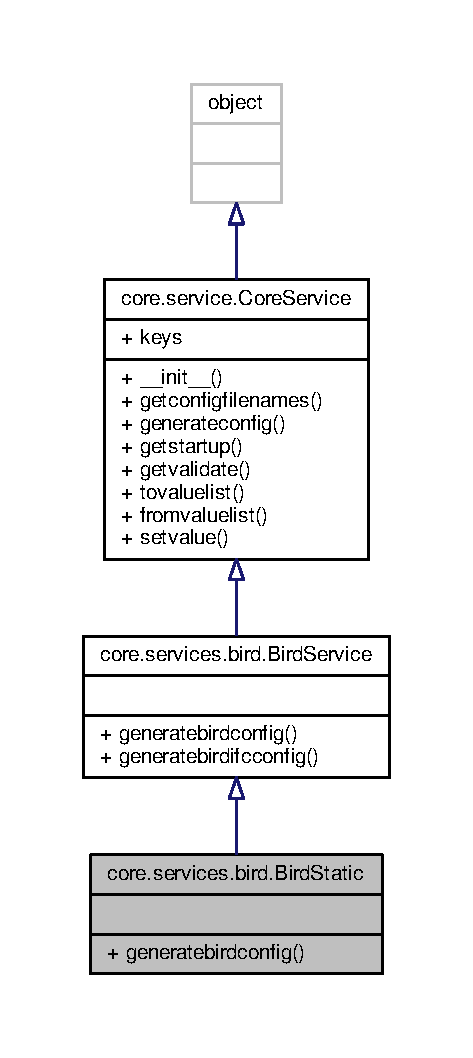
\includegraphics[width=227pt]{classcore_1_1services_1_1bird_1_1_bird_static__inherit__graph}
\end{center}
\end{figure}


Collaboration diagram for core.\+services.\+bird.\+Bird\+Static\+:
\nopagebreak
\begin{figure}[H]
\begin{center}
\leavevmode
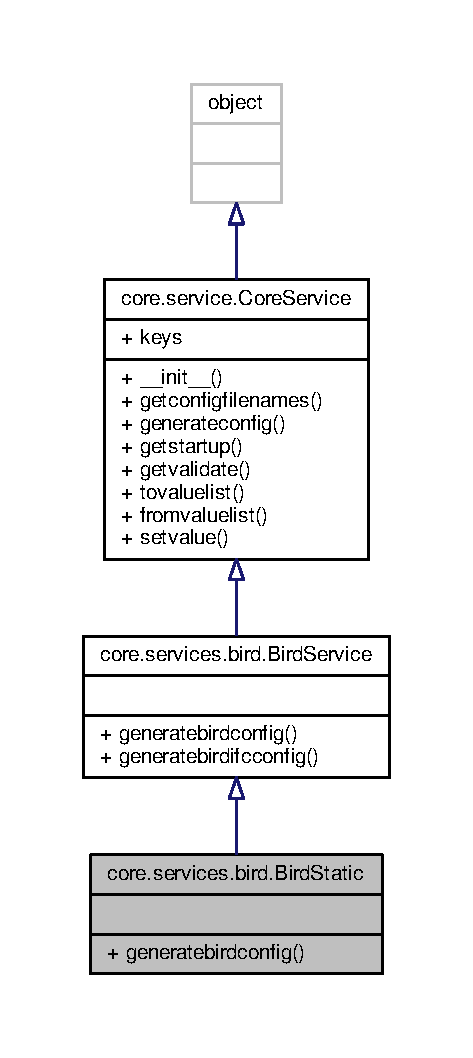
\includegraphics[width=227pt]{classcore_1_1services_1_1bird_1_1_bird_static__coll__graph}
\end{center}
\end{figure}
\subsection*{Public Member Functions}
\begin{DoxyCompactItemize}
\item 
\hypertarget{classcore_1_1services_1_1bird_1_1_bird_static_ab7e3c1e6ce131c1052f5f206a979588a}{def {\bfseries generatebirdconfig}}\label{classcore_1_1services_1_1bird_1_1_bird_static_ab7e3c1e6ce131c1052f5f206a979588a}

\end{DoxyCompactItemize}
\subsection*{Additional Inherited Members}


\subsection{Detailed Description}
\begin{DoxyVerb}Static Bird Service (configuration generation)\end{DoxyVerb}
 

The documentation for this class was generated from the following file\+:\begin{DoxyCompactItemize}
\item 
daemon/core/services/bird.\+py\end{DoxyCompactItemize}

\hypertarget{classcore_1_1sdt_1_1_sdt_1_1_bunch}{\section{core.\+sdt.\+Sdt.\+Bunch Class Reference}
\label{classcore_1_1sdt_1_1_sdt_1_1_bunch}\index{core.\+sdt.\+Sdt.\+Bunch@{core.\+sdt.\+Sdt.\+Bunch}}
}


Collaboration diagram for core.\+sdt.\+Sdt.\+Bunch\+:
\nopagebreak
\begin{figure}[H]
\begin{center}
\leavevmode
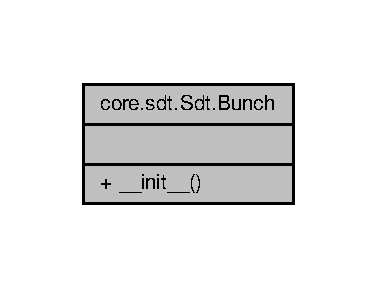
\includegraphics[width=181pt]{classcore_1_1sdt_1_1_sdt_1_1_bunch__coll__graph}
\end{center}
\end{figure}
\subsection*{Public Member Functions}
\begin{DoxyCompactItemize}
\item 
\hypertarget{classcore_1_1sdt_1_1_sdt_1_1_bunch_a7f605fab1cb780eefa73a7eae4016844}{def {\bfseries \+\_\+\+\_\+init\+\_\+\+\_\+}}\label{classcore_1_1sdt_1_1_sdt_1_1_bunch_a7f605fab1cb780eefa73a7eae4016844}

\end{DoxyCompactItemize}


\subsection{Detailed Description}
\begin{DoxyVerb}Helper class for recording a collection of attributes.
\end{DoxyVerb}
 

The documentation for this class was generated from the following file\+:\begin{DoxyCompactItemize}
\item 
daemon/core/sdt.\+py\end{DoxyCompactItemize}

\hypertarget{classcore_1_1misc_1_1xmlwriter1_1_1_channel_element}{\section{core.\+misc.\+xmlwriter1.\+Channel\+Element Class Reference}
\label{classcore_1_1misc_1_1xmlwriter1_1_1_channel_element}\index{core.\+misc.\+xmlwriter1.\+Channel\+Element@{core.\+misc.\+xmlwriter1.\+Channel\+Element}}
}


Inheritance diagram for core.\+misc.\+xmlwriter1.\+Channel\+Element\+:
\nopagebreak
\begin{figure}[H]
\begin{center}
\leavevmode
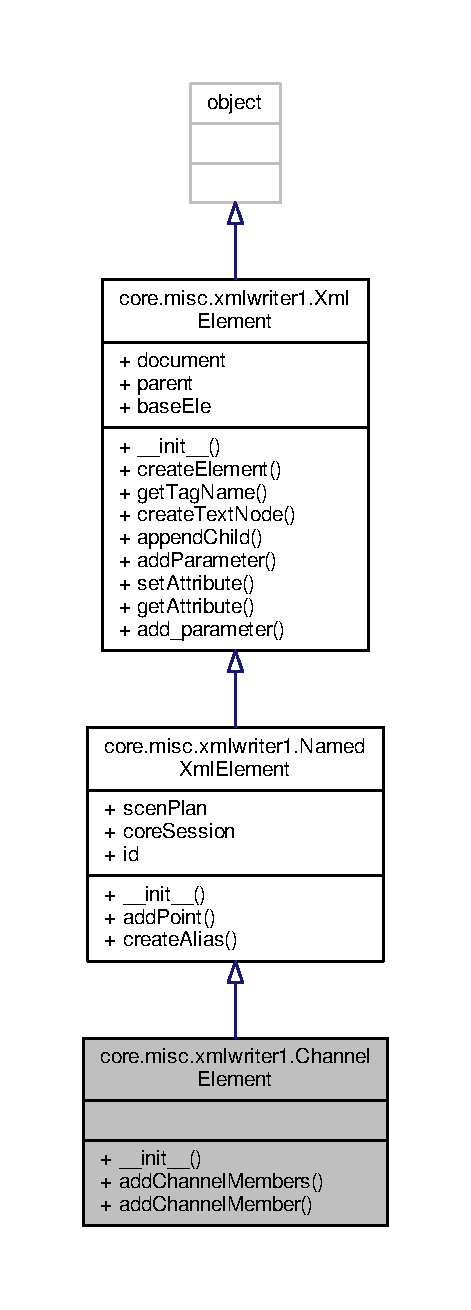
\includegraphics[height=550pt]{classcore_1_1misc_1_1xmlwriter1_1_1_channel_element__inherit__graph}
\end{center}
\end{figure}


Collaboration diagram for core.\+misc.\+xmlwriter1.\+Channel\+Element\+:
\nopagebreak
\begin{figure}[H]
\begin{center}
\leavevmode
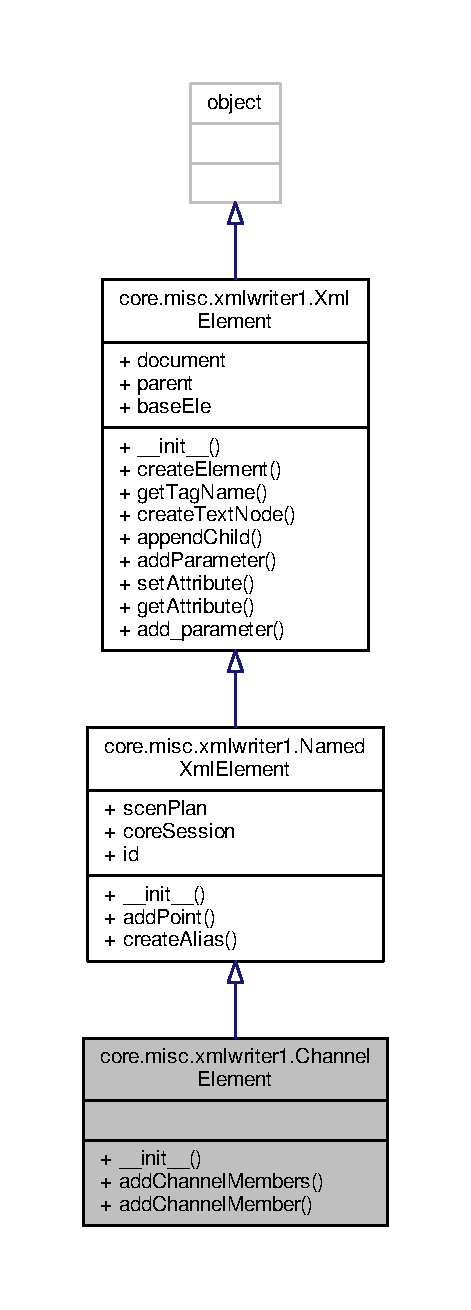
\includegraphics[height=550pt]{classcore_1_1misc_1_1xmlwriter1_1_1_channel_element__coll__graph}
\end{center}
\end{figure}
\subsection*{Public Member Functions}
\begin{DoxyCompactItemize}
\item 
\hypertarget{classcore_1_1misc_1_1xmlwriter1_1_1_channel_element_ad19c4403b3946420016504a52a6ce8ae}{def {\bfseries \+\_\+\+\_\+init\+\_\+\+\_\+}}\label{classcore_1_1misc_1_1xmlwriter1_1_1_channel_element_ad19c4403b3946420016504a52a6ce8ae}

\item 
def \hyperlink{classcore_1_1misc_1_1xmlwriter1_1_1_channel_element_a95eb20b81612b88d71acf5dd3085fdac}{add\+Channel\+Members}
\item 
def \hyperlink{classcore_1_1misc_1_1xmlwriter1_1_1_channel_element_a31222b4e6cfcbaa15360b294441435ef}{add\+Channel\+Member}
\end{DoxyCompactItemize}
\subsection*{Additional Inherited Members}


\subsection{Detailed Description}
\begin{DoxyVerb}A channel element in the scenario plan
\end{DoxyVerb}
 

\subsection{Member Function Documentation}
\hypertarget{classcore_1_1misc_1_1xmlwriter1_1_1_channel_element_a31222b4e6cfcbaa15360b294441435ef}{\index{core\+::misc\+::xmlwriter1\+::\+Channel\+Element@{core\+::misc\+::xmlwriter1\+::\+Channel\+Element}!add\+Channel\+Member@{add\+Channel\+Member}}
\index{add\+Channel\+Member@{add\+Channel\+Member}!core\+::misc\+::xmlwriter1\+::\+Channel\+Element@{core\+::misc\+::xmlwriter1\+::\+Channel\+Element}}
\subsubsection[{add\+Channel\+Member}]{\setlength{\rightskip}{0pt plus 5cm}def core.\+misc.\+xmlwriter1.\+Channel\+Element.\+add\+Channel\+Member (
\begin{DoxyParamCaption}
\item[{}]{self, }
\item[{}]{mem\+Ifc\+Type, }
\item[{}]{mem\+Ifc\+Id, }
\item[{}]{mem\+Idx}
\end{DoxyParamCaption}
)}}\label{classcore_1_1misc_1_1xmlwriter1_1_1_channel_element_a31222b4e6cfcbaa15360b294441435ef}
\begin{DoxyVerb}add a member to a given channel
\end{DoxyVerb}
 \hypertarget{classcore_1_1misc_1_1xmlwriter1_1_1_channel_element_a95eb20b81612b88d71acf5dd3085fdac}{\index{core\+::misc\+::xmlwriter1\+::\+Channel\+Element@{core\+::misc\+::xmlwriter1\+::\+Channel\+Element}!add\+Channel\+Members@{add\+Channel\+Members}}
\index{add\+Channel\+Members@{add\+Channel\+Members}!core\+::misc\+::xmlwriter1\+::\+Channel\+Element@{core\+::misc\+::xmlwriter1\+::\+Channel\+Element}}
\subsubsection[{add\+Channel\+Members}]{\setlength{\rightskip}{0pt plus 5cm}def core.\+misc.\+xmlwriter1.\+Channel\+Element.\+add\+Channel\+Members (
\begin{DoxyParamCaption}
\item[{}]{self, }
\item[{}]{endpoints}
\end{DoxyParamCaption}
)}}\label{classcore_1_1misc_1_1xmlwriter1_1_1_channel_element_a95eb20b81612b88d71acf5dd3085fdac}
\begin{DoxyVerb}Add network channel members referencing interfaces in the channel
\end{DoxyVerb}
 

The documentation for this class was generated from the following file\+:\begin{DoxyCompactItemize}
\item 
daemon/core/misc/xmlwriter1.\+py\end{DoxyCompactItemize}

\hypertarget{structcliententry}{\section{cliententry Struct Reference}
\label{structcliententry}\index{cliententry@{cliententry}}
}


Collaboration diagram for cliententry\+:
\nopagebreak
\begin{figure}[H]
\begin{center}
\leavevmode
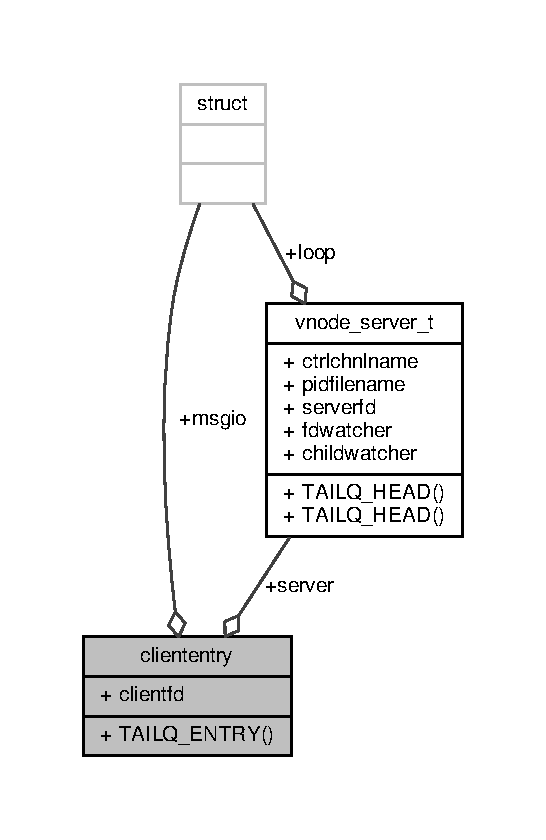
\includegraphics[width=262pt]{structcliententry__coll__graph}
\end{center}
\end{figure}
\subsection*{Public Member Functions}
\begin{DoxyCompactItemize}
\item 
\hypertarget{structcliententry_a0a69d40047ebfa79159dccaa10255be8}{{\bfseries T\+A\+I\+L\+Q\+\_\+\+E\+N\+T\+R\+Y} (\hyperlink{structcliententry}{cliententry}) entries}\label{structcliententry_a0a69d40047ebfa79159dccaa10255be8}

\end{DoxyCompactItemize}
\subsection*{Public Attributes}
\begin{DoxyCompactItemize}
\item 
\hypertarget{structcliententry_a8996f183f58a07f84728739dac2e88fc}{\hyperlink{structvnode__server__t}{vnode\+\_\+server\+\_\+t} $\ast$ {\bfseries server}}\label{structcliententry_a8996f183f58a07f84728739dac2e88fc}

\item 
\hypertarget{structcliententry_a5da0c8a9bf50b5c699745ab0f8fa41e8}{int {\bfseries clientfd}}\label{structcliententry_a5da0c8a9bf50b5c699745ab0f8fa41e8}

\item 
\hypertarget{structcliententry_a1ce643c3fb589997e9112f2d73213a97}{\hyperlink{structvnode__msgio}{vnode\+\_\+msgio\+\_\+t} {\bfseries msgio}}\label{structcliententry_a1ce643c3fb589997e9112f2d73213a97}

\end{DoxyCompactItemize}


The documentation for this struct was generated from the following file\+:\begin{DoxyCompactItemize}
\item 
daemon/src/vnode\+\_\+server.\+h\end{DoxyCompactItemize}

\hypertarget{classwlanemanetests_1_1_client_server_cmd}{\section{wlanemanetests.\+Client\+Server\+Cmd Class Reference}
\label{classwlanemanetests_1_1_client_server_cmd}\index{wlanemanetests.\+Client\+Server\+Cmd@{wlanemanetests.\+Client\+Server\+Cmd}}
}


Inheritance diagram for wlanemanetests.\+Client\+Server\+Cmd\+:
\nopagebreak
\begin{figure}[H]
\begin{center}
\leavevmode
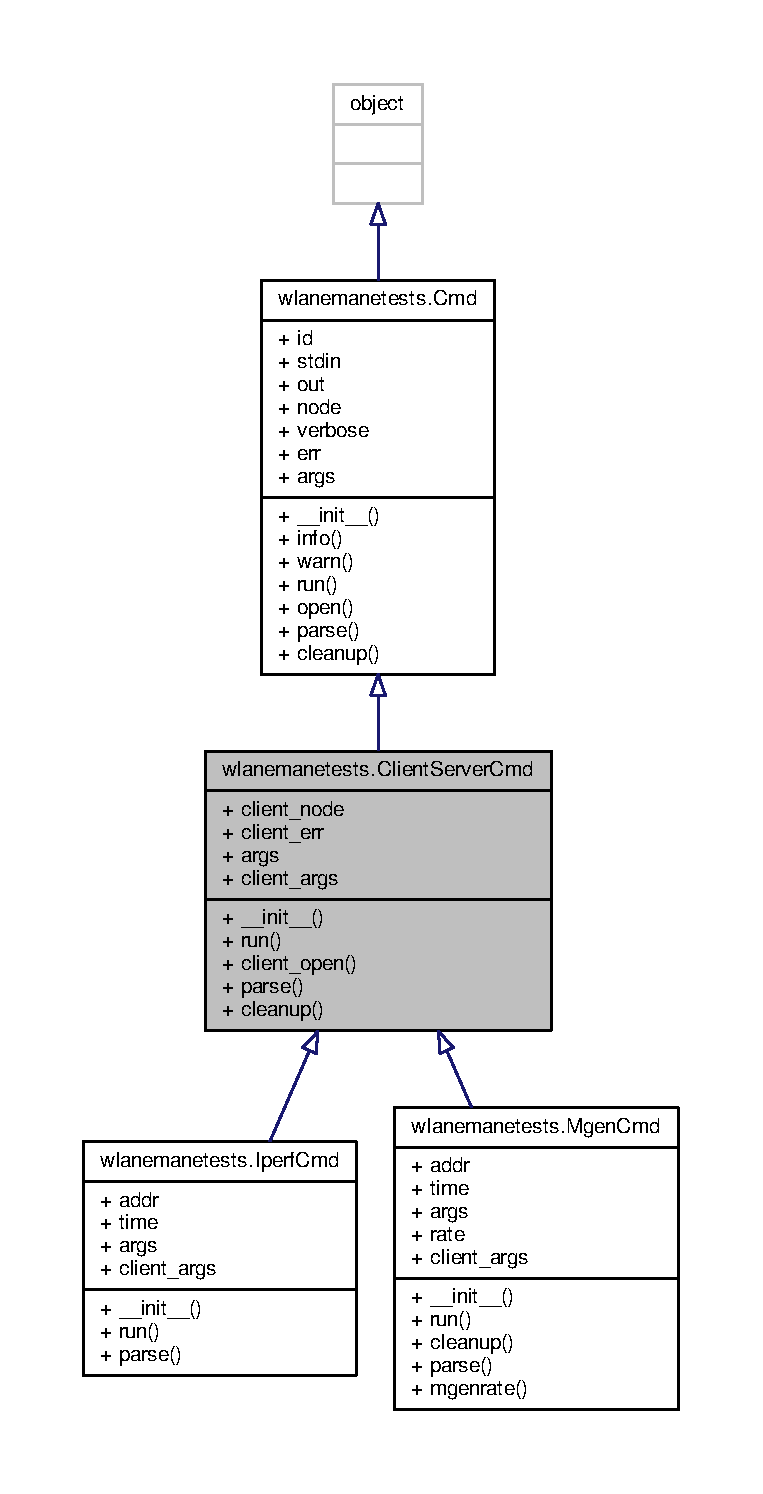
\includegraphics[height=550pt]{classwlanemanetests_1_1_client_server_cmd__inherit__graph}
\end{center}
\end{figure}


Collaboration diagram for wlanemanetests.\+Client\+Server\+Cmd\+:
\nopagebreak
\begin{figure}[H]
\begin{center}
\leavevmode
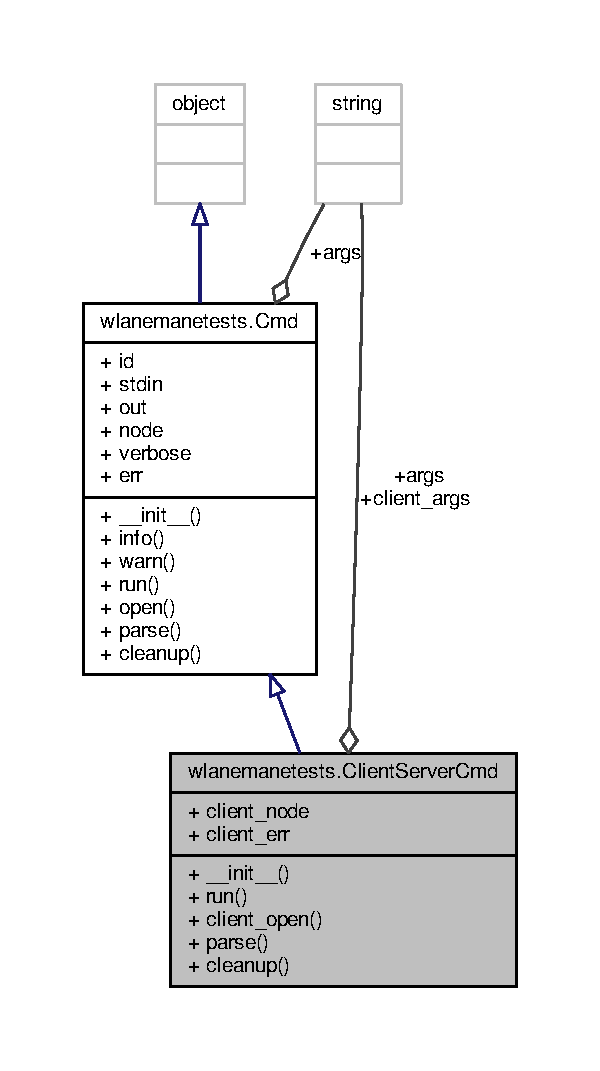
\includegraphics[width=288pt]{classwlanemanetests_1_1_client_server_cmd__coll__graph}
\end{center}
\end{figure}
\subsection*{Public Member Functions}
\begin{DoxyCompactItemize}
\item 
def \hyperlink{classwlanemanetests_1_1_client_server_cmd_a6147b9c996e41c83f8ebbb81f5aee5be}{\+\_\+\+\_\+init\+\_\+\+\_\+}
\item 
def \hyperlink{classwlanemanetests_1_1_client_server_cmd_ac5c400fc3217b84d5e708486fe160bea}{run}
\item 
def \hyperlink{classwlanemanetests_1_1_client_server_cmd_a3c60da372a7c98838e9fdf0ce7a9e9cf}{client\+\_\+open}
\item 
def \hyperlink{classwlanemanetests_1_1_client_server_cmd_af9f71c30e89e355a343a6c1df78e599a}{parse}
\item 
def \hyperlink{classwlanemanetests_1_1_client_server_cmd_a10ed475cfd9e8db2e7cd52a0310af91b}{cleanup}
\end{DoxyCompactItemize}
\subsection*{Public Attributes}
\begin{DoxyCompactItemize}
\item 
\hypertarget{classwlanemanetests_1_1_client_server_cmd_a874b7f85c3316c69f940bebb4afea9d7}{{\bfseries client\+\_\+node}}\label{classwlanemanetests_1_1_client_server_cmd_a874b7f85c3316c69f940bebb4afea9d7}

\item 
\hypertarget{classwlanemanetests_1_1_client_server_cmd_a43ec35ad1998a901f7a789c8b93698f6}{{\bfseries client\+\_\+err}}\label{classwlanemanetests_1_1_client_server_cmd_a43ec35ad1998a901f7a789c8b93698f6}

\end{DoxyCompactItemize}
\subsection*{Static Public Attributes}
\begin{DoxyCompactItemize}
\item 
\hypertarget{classwlanemanetests_1_1_client_server_cmd_a6540d3c6444bca3589109c138db8a235}{string {\bfseries args} = \char`\"{}\char`\"{}}\label{classwlanemanetests_1_1_client_server_cmd_a6540d3c6444bca3589109c138db8a235}

\item 
\hypertarget{classwlanemanetests_1_1_client_server_cmd_ab612f0a4e42a37fdf10a1943fa4c73b0}{string {\bfseries client\+\_\+args} = \char`\"{}\char`\"{}}\label{classwlanemanetests_1_1_client_server_cmd_ab612f0a4e42a37fdf10a1943fa4c73b0}

\end{DoxyCompactItemize}


\subsection{Detailed Description}
\begin{DoxyVerb}Helper class for running a command on a node and parsing the result. \end{DoxyVerb}
 

\subsection{Constructor \& Destructor Documentation}
\hypertarget{classwlanemanetests_1_1_client_server_cmd_a6147b9c996e41c83f8ebbb81f5aee5be}{\index{wlanemanetests\+::\+Client\+Server\+Cmd@{wlanemanetests\+::\+Client\+Server\+Cmd}!\+\_\+\+\_\+init\+\_\+\+\_\+@{\+\_\+\+\_\+init\+\_\+\+\_\+}}
\index{\+\_\+\+\_\+init\+\_\+\+\_\+@{\+\_\+\+\_\+init\+\_\+\+\_\+}!wlanemanetests\+::\+Client\+Server\+Cmd@{wlanemanetests\+::\+Client\+Server\+Cmd}}
\subsubsection[{\+\_\+\+\_\+init\+\_\+\+\_\+}]{\setlength{\rightskip}{0pt plus 5cm}def wlanemanetests.\+Client\+Server\+Cmd.\+\_\+\+\_\+init\+\_\+\+\_\+ (
\begin{DoxyParamCaption}
\item[{}]{self, }
\item[{}]{node, }
\item[{}]{client\+\_\+node, }
\item[{}]{verbose = {\ttfamily False}}
\end{DoxyParamCaption}
)}}\label{classwlanemanetests_1_1_client_server_cmd_a6147b9c996e41c83f8ebbb81f5aee5be}
\begin{DoxyVerb}Initialize with two CoreNodes, node is the server \end{DoxyVerb}
 

\subsection{Member Function Documentation}
\hypertarget{classwlanemanetests_1_1_client_server_cmd_a10ed475cfd9e8db2e7cd52a0310af91b}{\index{wlanemanetests\+::\+Client\+Server\+Cmd@{wlanemanetests\+::\+Client\+Server\+Cmd}!cleanup@{cleanup}}
\index{cleanup@{cleanup}!wlanemanetests\+::\+Client\+Server\+Cmd@{wlanemanetests\+::\+Client\+Server\+Cmd}}
\subsubsection[{cleanup}]{\setlength{\rightskip}{0pt plus 5cm}def wlanemanetests.\+Client\+Server\+Cmd.\+cleanup (
\begin{DoxyParamCaption}
\item[{}]{self}
\end{DoxyParamCaption}
)}}\label{classwlanemanetests_1_1_client_server_cmd_a10ed475cfd9e8db2e7cd52a0310af91b}
\begin{DoxyVerb}Close the Popen channels.\end{DoxyVerb}
 \hypertarget{classwlanemanetests_1_1_client_server_cmd_a3c60da372a7c98838e9fdf0ce7a9e9cf}{\index{wlanemanetests\+::\+Client\+Server\+Cmd@{wlanemanetests\+::\+Client\+Server\+Cmd}!client\+\_\+open@{client\+\_\+open}}
\index{client\+\_\+open@{client\+\_\+open}!wlanemanetests\+::\+Client\+Server\+Cmd@{wlanemanetests\+::\+Client\+Server\+Cmd}}
\subsubsection[{client\+\_\+open}]{\setlength{\rightskip}{0pt plus 5cm}def wlanemanetests.\+Client\+Server\+Cmd.\+client\+\_\+open (
\begin{DoxyParamCaption}
\item[{}]{self}
\end{DoxyParamCaption}
)}}\label{classwlanemanetests_1_1_client_server_cmd_a3c60da372a7c98838e9fdf0ce7a9e9cf}
\begin{DoxyVerb}Exceute call to client_node.popen(). \end{DoxyVerb}
 \hypertarget{classwlanemanetests_1_1_client_server_cmd_af9f71c30e89e355a343a6c1df78e599a}{\index{wlanemanetests\+::\+Client\+Server\+Cmd@{wlanemanetests\+::\+Client\+Server\+Cmd}!parse@{parse}}
\index{parse@{parse}!wlanemanetests\+::\+Client\+Server\+Cmd@{wlanemanetests\+::\+Client\+Server\+Cmd}}
\subsubsection[{parse}]{\setlength{\rightskip}{0pt plus 5cm}def wlanemanetests.\+Client\+Server\+Cmd.\+parse (
\begin{DoxyParamCaption}
\item[{}]{self}
\end{DoxyParamCaption}
)}}\label{classwlanemanetests_1_1_client_server_cmd_af9f71c30e89e355a343a6c1df78e599a}
\begin{DoxyVerb}This method is overloaded by child classes and should return some
    result.
\end{DoxyVerb}
 \hypertarget{classwlanemanetests_1_1_client_server_cmd_ac5c400fc3217b84d5e708486fe160bea}{\index{wlanemanetests\+::\+Client\+Server\+Cmd@{wlanemanetests\+::\+Client\+Server\+Cmd}!run@{run}}
\index{run@{run}!wlanemanetests\+::\+Client\+Server\+Cmd@{wlanemanetests\+::\+Client\+Server\+Cmd}}
\subsubsection[{run}]{\setlength{\rightskip}{0pt plus 5cm}def wlanemanetests.\+Client\+Server\+Cmd.\+run (
\begin{DoxyParamCaption}
\item[{}]{self}
\end{DoxyParamCaption}
)}}\label{classwlanemanetests_1_1_client_server_cmd_ac5c400fc3217b84d5e708486fe160bea}
\begin{DoxyVerb}Run the server command, then the client command, then
kill the server \end{DoxyVerb}
 

The documentation for this class was generated from the following file\+:\begin{DoxyCompactItemize}
\item 
daemon/examples/netns/wlanemanetests.\+py\end{DoxyCompactItemize}

\hypertarget{classospfmanetmdrtest_1_1_cmd}{\section{ospfmanetmdrtest.\+Cmd Class Reference}
\label{classospfmanetmdrtest_1_1_cmd}\index{ospfmanetmdrtest.\+Cmd@{ospfmanetmdrtest.\+Cmd}}
}


Inheritance diagram for ospfmanetmdrtest.\+Cmd\+:
\nopagebreak
\begin{figure}[H]
\begin{center}
\leavevmode
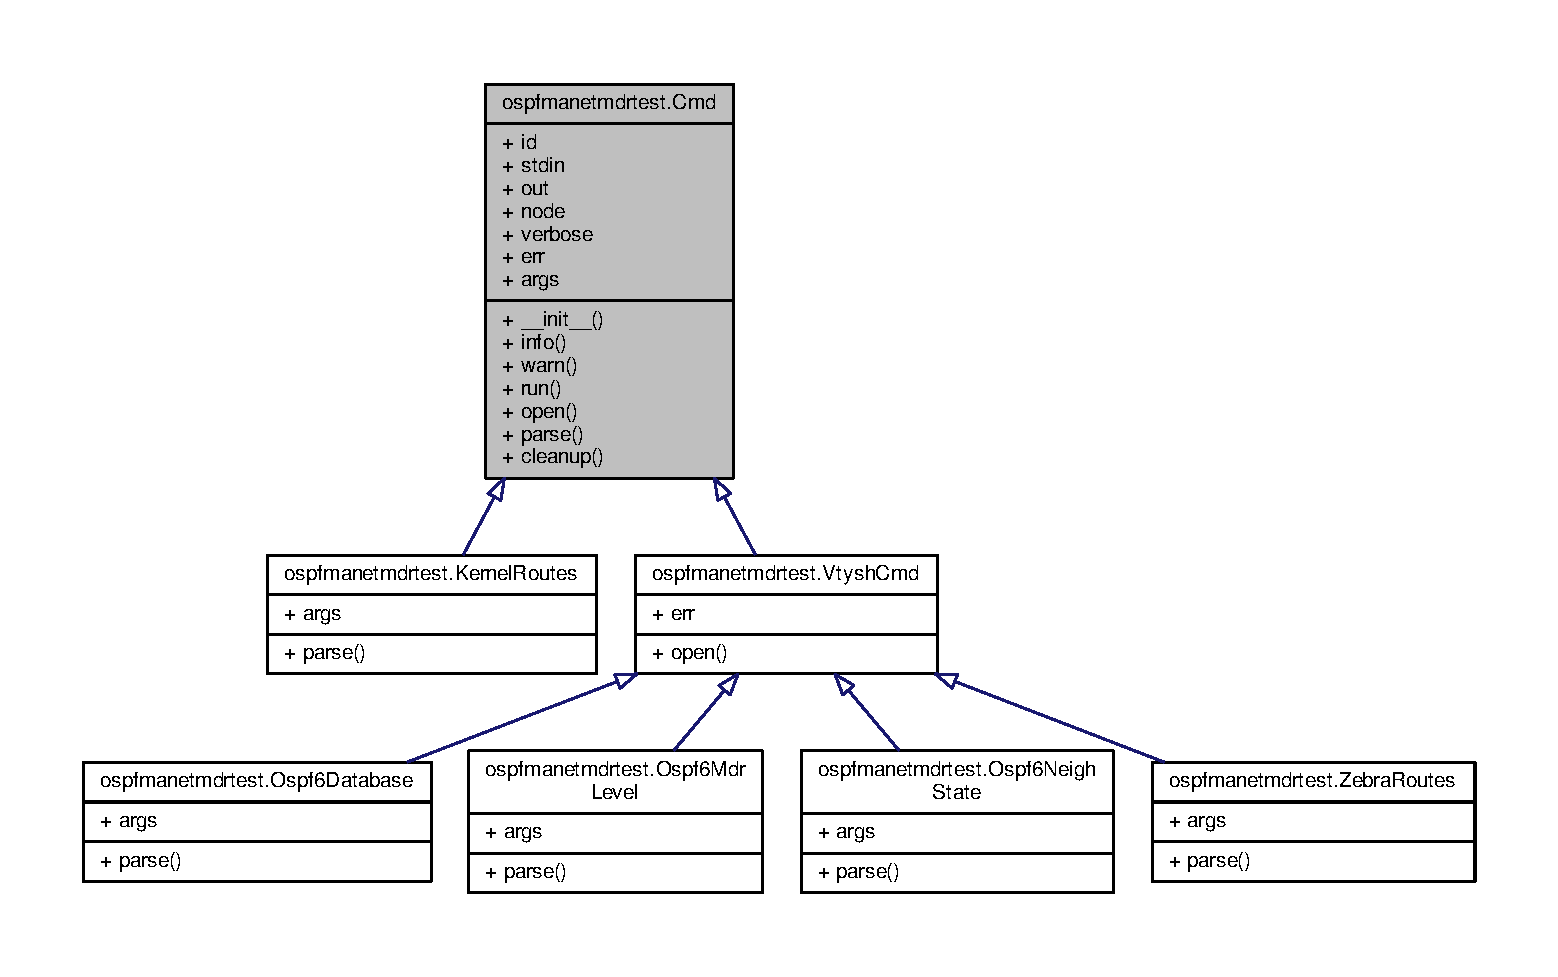
\includegraphics[width=350pt]{classospfmanetmdrtest_1_1_cmd__inherit__graph}
\end{center}
\end{figure}


Collaboration diagram for ospfmanetmdrtest.\+Cmd\+:
\nopagebreak
\begin{figure}[H]
\begin{center}
\leavevmode
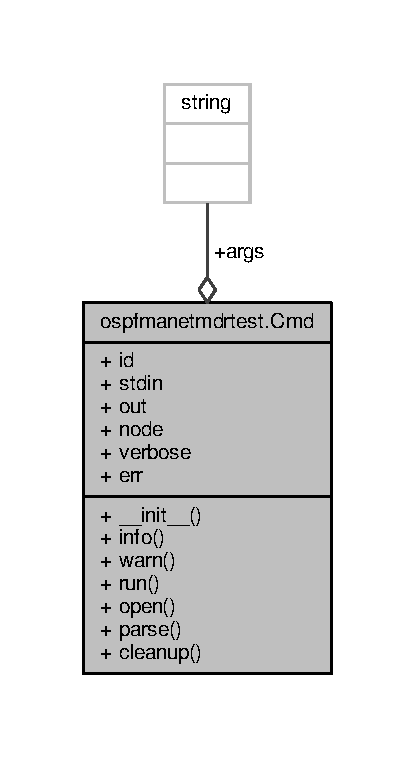
\includegraphics[width=199pt]{classospfmanetmdrtest_1_1_cmd__coll__graph}
\end{center}
\end{figure}
\subsection*{Public Member Functions}
\begin{DoxyCompactItemize}
\item 
def \hyperlink{classospfmanetmdrtest_1_1_cmd_ab02c7cf620600e31b76f667fd420f317}{\+\_\+\+\_\+init\+\_\+\+\_\+}
\item 
def \hyperlink{classospfmanetmdrtest_1_1_cmd_a5506910c4ded480c95053a9c633ae79d}{info}
\item 
def \hyperlink{classospfmanetmdrtest_1_1_cmd_a413e3dbfe7c5508f069ff4f06ce3d51f}{warn}
\item 
def \hyperlink{classospfmanetmdrtest_1_1_cmd_ac598d665a861a9ec683f1965bbb91d03}{run}
\item 
def \hyperlink{classospfmanetmdrtest_1_1_cmd_ac5fa80184c4322ab00b294eafa593b25}{open}
\item 
def \hyperlink{classospfmanetmdrtest_1_1_cmd_aa17319b4967ea4eba32a70a6afbe38d3}{parse}
\item 
def \hyperlink{classospfmanetmdrtest_1_1_cmd_ad6618fcdebb8d6da31267082ad2e65bc}{cleanup}
\end{DoxyCompactItemize}
\subsection*{Public Attributes}
\begin{DoxyCompactItemize}
\item 
\hypertarget{classospfmanetmdrtest_1_1_cmd_a8e8dc7a079c3aba53fb551ce873b62ba}{{\bfseries id}}\label{classospfmanetmdrtest_1_1_cmd_a8e8dc7a079c3aba53fb551ce873b62ba}

\item 
\hypertarget{classospfmanetmdrtest_1_1_cmd_a9c6143f1aec039c58db94d916f2af939}{{\bfseries stdin}}\label{classospfmanetmdrtest_1_1_cmd_a9c6143f1aec039c58db94d916f2af939}

\item 
\hypertarget{classospfmanetmdrtest_1_1_cmd_a33a089b0504e3732504d0576180daa75}{{\bfseries out}}\label{classospfmanetmdrtest_1_1_cmd_a33a089b0504e3732504d0576180daa75}

\item 
\hypertarget{classospfmanetmdrtest_1_1_cmd_afed2fa10c1050eb92be08715423ebb78}{{\bfseries node}}\label{classospfmanetmdrtest_1_1_cmd_afed2fa10c1050eb92be08715423ebb78}

\item 
\hypertarget{classospfmanetmdrtest_1_1_cmd_ae89258a5b47a0c9e8f8fd3f01c82500a}{{\bfseries verbose}}\label{classospfmanetmdrtest_1_1_cmd_ae89258a5b47a0c9e8f8fd3f01c82500a}

\item 
\hypertarget{classospfmanetmdrtest_1_1_cmd_a44555b79a7cd44558de31cb121cf913e}{{\bfseries err}}\label{classospfmanetmdrtest_1_1_cmd_a44555b79a7cd44558de31cb121cf913e}

\end{DoxyCompactItemize}
\subsection*{Static Public Attributes}
\begin{DoxyCompactItemize}
\item 
\hypertarget{classospfmanetmdrtest_1_1_cmd_ac5b4466273e34e9f00474f33f7953943}{string {\bfseries args} = \char`\"{}\char`\"{}}\label{classospfmanetmdrtest_1_1_cmd_ac5b4466273e34e9f00474f33f7953943}

\end{DoxyCompactItemize}


\subsection{Detailed Description}
\begin{DoxyVerb}Helper class for running a command on a node and parsing the result. \end{DoxyVerb}
 

\subsection{Constructor \& Destructor Documentation}
\hypertarget{classospfmanetmdrtest_1_1_cmd_ab02c7cf620600e31b76f667fd420f317}{\index{ospfmanetmdrtest\+::\+Cmd@{ospfmanetmdrtest\+::\+Cmd}!\+\_\+\+\_\+init\+\_\+\+\_\+@{\+\_\+\+\_\+init\+\_\+\+\_\+}}
\index{\+\_\+\+\_\+init\+\_\+\+\_\+@{\+\_\+\+\_\+init\+\_\+\+\_\+}!ospfmanetmdrtest\+::\+Cmd@{ospfmanetmdrtest\+::\+Cmd}}
\subsubsection[{\+\_\+\+\_\+init\+\_\+\+\_\+}]{\setlength{\rightskip}{0pt plus 5cm}def ospfmanetmdrtest.\+Cmd.\+\_\+\+\_\+init\+\_\+\+\_\+ (
\begin{DoxyParamCaption}
\item[{}]{self, }
\item[{}]{node, }
\item[{}]{verbose = {\ttfamily False}}
\end{DoxyParamCaption}
)}}\label{classospfmanetmdrtest_1_1_cmd_ab02c7cf620600e31b76f667fd420f317}
\begin{DoxyVerb}Initialize with a CoreNode (LxcNode) \end{DoxyVerb}
 

\subsection{Member Function Documentation}
\hypertarget{classospfmanetmdrtest_1_1_cmd_ad6618fcdebb8d6da31267082ad2e65bc}{\index{ospfmanetmdrtest\+::\+Cmd@{ospfmanetmdrtest\+::\+Cmd}!cleanup@{cleanup}}
\index{cleanup@{cleanup}!ospfmanetmdrtest\+::\+Cmd@{ospfmanetmdrtest\+::\+Cmd}}
\subsubsection[{cleanup}]{\setlength{\rightskip}{0pt plus 5cm}def ospfmanetmdrtest.\+Cmd.\+cleanup (
\begin{DoxyParamCaption}
\item[{}]{self}
\end{DoxyParamCaption}
)}}\label{classospfmanetmdrtest_1_1_cmd_ad6618fcdebb8d6da31267082ad2e65bc}
\begin{DoxyVerb}Close the Popen channels.\end{DoxyVerb}
 \hypertarget{classospfmanetmdrtest_1_1_cmd_a5506910c4ded480c95053a9c633ae79d}{\index{ospfmanetmdrtest\+::\+Cmd@{ospfmanetmdrtest\+::\+Cmd}!info@{info}}
\index{info@{info}!ospfmanetmdrtest\+::\+Cmd@{ospfmanetmdrtest\+::\+Cmd}}
\subsubsection[{info}]{\setlength{\rightskip}{0pt plus 5cm}def ospfmanetmdrtest.\+Cmd.\+info (
\begin{DoxyParamCaption}
\item[{}]{self, }
\item[{}]{msg}
\end{DoxyParamCaption}
)}}\label{classospfmanetmdrtest_1_1_cmd_a5506910c4ded480c95053a9c633ae79d}
\begin{DoxyVerb}Utility method for writing output to stdout.\end{DoxyVerb}
 \hypertarget{classospfmanetmdrtest_1_1_cmd_ac5fa80184c4322ab00b294eafa593b25}{\index{ospfmanetmdrtest\+::\+Cmd@{ospfmanetmdrtest\+::\+Cmd}!open@{open}}
\index{open@{open}!ospfmanetmdrtest\+::\+Cmd@{ospfmanetmdrtest\+::\+Cmd}}
\subsubsection[{open}]{\setlength{\rightskip}{0pt plus 5cm}def ospfmanetmdrtest.\+Cmd.\+open (
\begin{DoxyParamCaption}
\item[{}]{self}
\end{DoxyParamCaption}
)}}\label{classospfmanetmdrtest_1_1_cmd_ac5fa80184c4322ab00b294eafa593b25}
\begin{DoxyVerb}Exceute call to node.popen(). \end{DoxyVerb}
 \hypertarget{classospfmanetmdrtest_1_1_cmd_aa17319b4967ea4eba32a70a6afbe38d3}{\index{ospfmanetmdrtest\+::\+Cmd@{ospfmanetmdrtest\+::\+Cmd}!parse@{parse}}
\index{parse@{parse}!ospfmanetmdrtest\+::\+Cmd@{ospfmanetmdrtest\+::\+Cmd}}
\subsubsection[{parse}]{\setlength{\rightskip}{0pt plus 5cm}def ospfmanetmdrtest.\+Cmd.\+parse (
\begin{DoxyParamCaption}
\item[{}]{self}
\end{DoxyParamCaption}
)}}\label{classospfmanetmdrtest_1_1_cmd_aa17319b4967ea4eba32a70a6afbe38d3}
\begin{DoxyVerb}This method is overloaded by child classes and should return some
    result.
\end{DoxyVerb}
 \hypertarget{classospfmanetmdrtest_1_1_cmd_ac598d665a861a9ec683f1965bbb91d03}{\index{ospfmanetmdrtest\+::\+Cmd@{ospfmanetmdrtest\+::\+Cmd}!run@{run}}
\index{run@{run}!ospfmanetmdrtest\+::\+Cmd@{ospfmanetmdrtest\+::\+Cmd}}
\subsubsection[{run}]{\setlength{\rightskip}{0pt plus 5cm}def ospfmanetmdrtest.\+Cmd.\+run (
\begin{DoxyParamCaption}
\item[{}]{self}
\end{DoxyParamCaption}
)}}\label{classospfmanetmdrtest_1_1_cmd_ac598d665a861a9ec683f1965bbb91d03}
\begin{DoxyVerb}This is the primary method used for running this command. \end{DoxyVerb}
 \hypertarget{classospfmanetmdrtest_1_1_cmd_a413e3dbfe7c5508f069ff4f06ce3d51f}{\index{ospfmanetmdrtest\+::\+Cmd@{ospfmanetmdrtest\+::\+Cmd}!warn@{warn}}
\index{warn@{warn}!ospfmanetmdrtest\+::\+Cmd@{ospfmanetmdrtest\+::\+Cmd}}
\subsubsection[{warn}]{\setlength{\rightskip}{0pt plus 5cm}def ospfmanetmdrtest.\+Cmd.\+warn (
\begin{DoxyParamCaption}
\item[{}]{self, }
\item[{}]{msg}
\end{DoxyParamCaption}
)}}\label{classospfmanetmdrtest_1_1_cmd_a413e3dbfe7c5508f069ff4f06ce3d51f}
\begin{DoxyVerb}Utility method for writing output to stderr. \end{DoxyVerb}
 

The documentation for this class was generated from the following file\+:\begin{DoxyCompactItemize}
\item 
daemon/examples/netns/ospfmanetmdrtest.\+py\end{DoxyCompactItemize}

\hypertarget{classwlanemanetests_1_1_cmd}{\section{wlanemanetests.\+Cmd Class Reference}
\label{classwlanemanetests_1_1_cmd}\index{wlanemanetests.\+Cmd@{wlanemanetests.\+Cmd}}
}


Inheritance diagram for wlanemanetests.\+Cmd\+:
\nopagebreak
\begin{figure}[H]
\begin{center}
\leavevmode
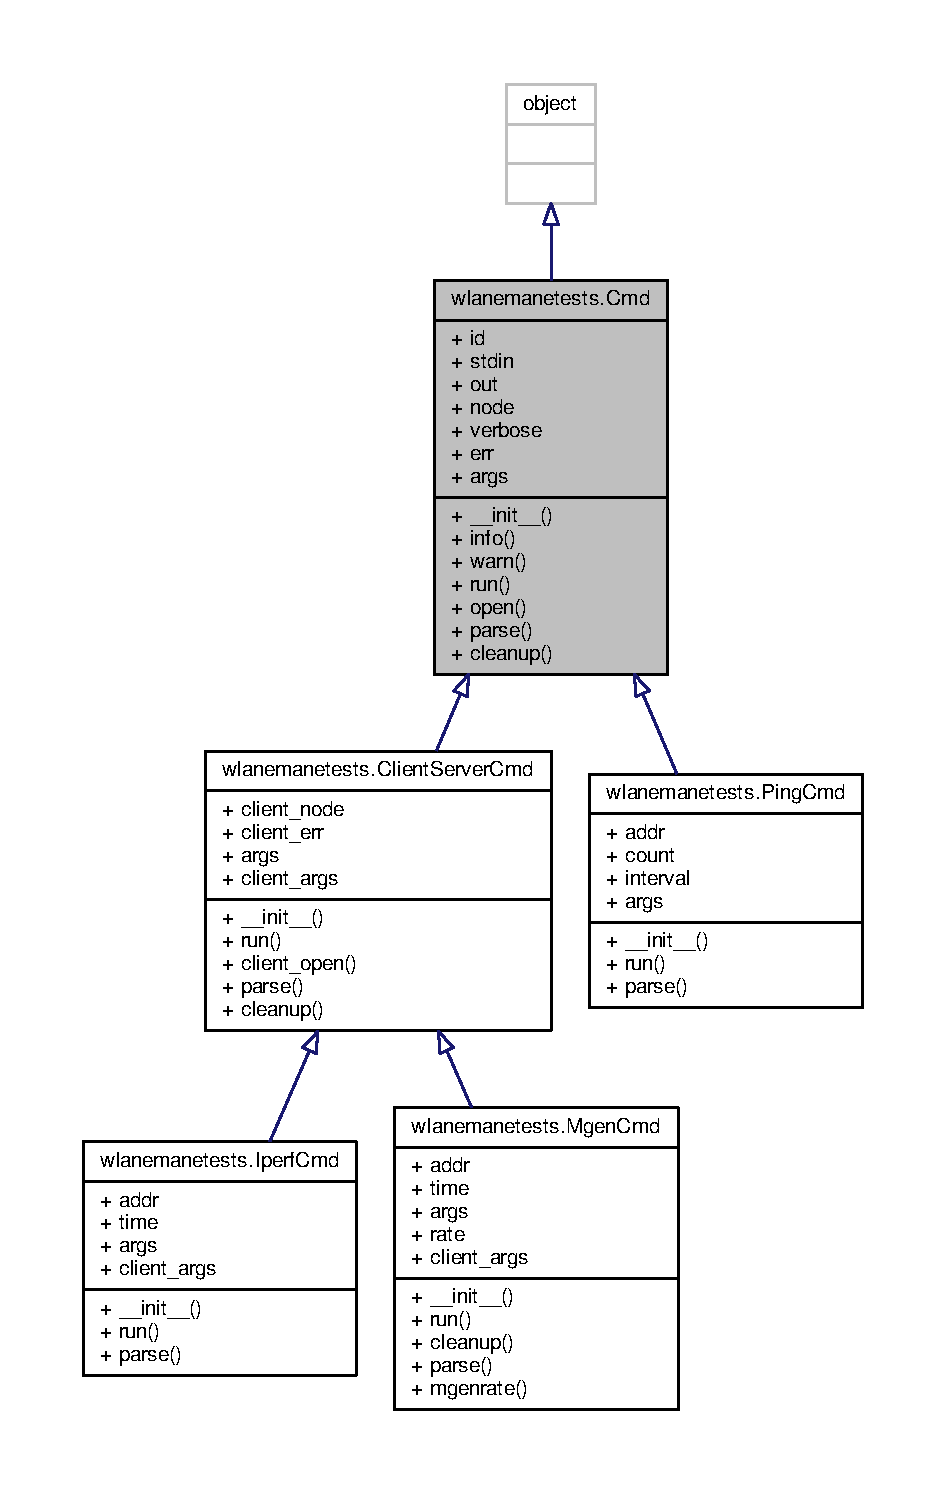
\includegraphics[height=550pt]{classwlanemanetests_1_1_cmd__inherit__graph}
\end{center}
\end{figure}


Collaboration diagram for wlanemanetests.\+Cmd\+:
\nopagebreak
\begin{figure}[H]
\begin{center}
\leavevmode
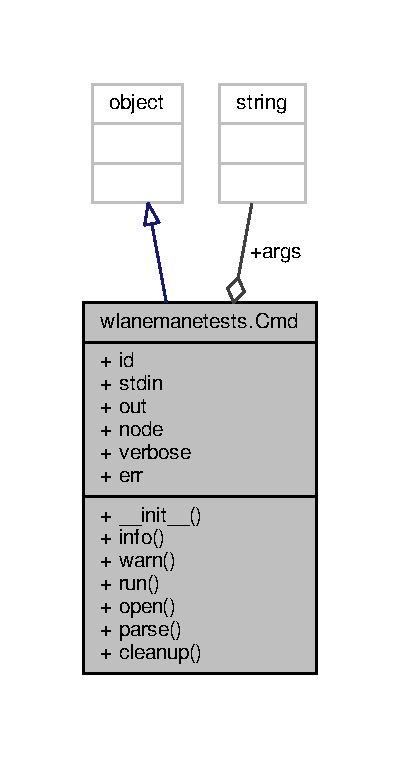
\includegraphics[width=192pt]{classwlanemanetests_1_1_cmd__coll__graph}
\end{center}
\end{figure}
\subsection*{Public Member Functions}
\begin{DoxyCompactItemize}
\item 
def \hyperlink{classwlanemanetests_1_1_cmd_acd8fc0a7579f5e2f12875ddfbafa5382}{\+\_\+\+\_\+init\+\_\+\+\_\+}
\item 
def \hyperlink{classwlanemanetests_1_1_cmd_a6b12b2c0c67f717c73292b5dd4220763}{info}
\item 
def \hyperlink{classwlanemanetests_1_1_cmd_ac5a04cd30be3cce2e85be31167112d95}{warn}
\item 
def \hyperlink{classwlanemanetests_1_1_cmd_a16f428c0a4dff9a7295e11b47350af29}{run}
\item 
def \hyperlink{classwlanemanetests_1_1_cmd_a528f6b2acf2d5c8e40af98a32dd3b73a}{open}
\item 
def \hyperlink{classwlanemanetests_1_1_cmd_a416225dd2ad7a266d7252602aaaef2e2}{parse}
\item 
def \hyperlink{classwlanemanetests_1_1_cmd_a87a05cf4e6499cd488ed5194344795ae}{cleanup}
\end{DoxyCompactItemize}
\subsection*{Public Attributes}
\begin{DoxyCompactItemize}
\item 
\hypertarget{classwlanemanetests_1_1_cmd_a0729e986a24c999ccb476131aa645ad5}{{\bfseries id}}\label{classwlanemanetests_1_1_cmd_a0729e986a24c999ccb476131aa645ad5}

\item 
\hypertarget{classwlanemanetests_1_1_cmd_a2957c29f4038ba406d76646e51945583}{{\bfseries stdin}}\label{classwlanemanetests_1_1_cmd_a2957c29f4038ba406d76646e51945583}

\item 
\hypertarget{classwlanemanetests_1_1_cmd_a2f5641b4556d6d84df3b1c0f3a3cf3e2}{{\bfseries out}}\label{classwlanemanetests_1_1_cmd_a2f5641b4556d6d84df3b1c0f3a3cf3e2}

\item 
\hypertarget{classwlanemanetests_1_1_cmd_a7ef748d8e0ee897ad31dbf4847f89def}{{\bfseries node}}\label{classwlanemanetests_1_1_cmd_a7ef748d8e0ee897ad31dbf4847f89def}

\item 
\hypertarget{classwlanemanetests_1_1_cmd_adad2980a0733d953b097dcb94946e9fa}{{\bfseries verbose}}\label{classwlanemanetests_1_1_cmd_adad2980a0733d953b097dcb94946e9fa}

\item 
\hypertarget{classwlanemanetests_1_1_cmd_aee35a55395cb66e2ad8f51b862a179b4}{{\bfseries err}}\label{classwlanemanetests_1_1_cmd_aee35a55395cb66e2ad8f51b862a179b4}

\end{DoxyCompactItemize}
\subsection*{Static Public Attributes}
\begin{DoxyCompactItemize}
\item 
\hypertarget{classwlanemanetests_1_1_cmd_a4788170395862e1b4e28f7a9274764d4}{string {\bfseries args} = \char`\"{}\char`\"{}}\label{classwlanemanetests_1_1_cmd_a4788170395862e1b4e28f7a9274764d4}

\end{DoxyCompactItemize}


\subsection{Detailed Description}
\begin{DoxyVerb}Helper class for running a command on a node and parsing the result. \end{DoxyVerb}
 

\subsection{Constructor \& Destructor Documentation}
\hypertarget{classwlanemanetests_1_1_cmd_acd8fc0a7579f5e2f12875ddfbafa5382}{\index{wlanemanetests\+::\+Cmd@{wlanemanetests\+::\+Cmd}!\+\_\+\+\_\+init\+\_\+\+\_\+@{\+\_\+\+\_\+init\+\_\+\+\_\+}}
\index{\+\_\+\+\_\+init\+\_\+\+\_\+@{\+\_\+\+\_\+init\+\_\+\+\_\+}!wlanemanetests\+::\+Cmd@{wlanemanetests\+::\+Cmd}}
\subsubsection[{\+\_\+\+\_\+init\+\_\+\+\_\+}]{\setlength{\rightskip}{0pt plus 5cm}def wlanemanetests.\+Cmd.\+\_\+\+\_\+init\+\_\+\+\_\+ (
\begin{DoxyParamCaption}
\item[{}]{self, }
\item[{}]{node, }
\item[{}]{verbose = {\ttfamily False}}
\end{DoxyParamCaption}
)}}\label{classwlanemanetests_1_1_cmd_acd8fc0a7579f5e2f12875ddfbafa5382}
\begin{DoxyVerb}Initialize with a CoreNode (LxcNode) \end{DoxyVerb}
 

\subsection{Member Function Documentation}
\hypertarget{classwlanemanetests_1_1_cmd_a87a05cf4e6499cd488ed5194344795ae}{\index{wlanemanetests\+::\+Cmd@{wlanemanetests\+::\+Cmd}!cleanup@{cleanup}}
\index{cleanup@{cleanup}!wlanemanetests\+::\+Cmd@{wlanemanetests\+::\+Cmd}}
\subsubsection[{cleanup}]{\setlength{\rightskip}{0pt plus 5cm}def wlanemanetests.\+Cmd.\+cleanup (
\begin{DoxyParamCaption}
\item[{}]{self}
\end{DoxyParamCaption}
)}}\label{classwlanemanetests_1_1_cmd_a87a05cf4e6499cd488ed5194344795ae}
\begin{DoxyVerb}Close the Popen channels.\end{DoxyVerb}
 \hypertarget{classwlanemanetests_1_1_cmd_a6b12b2c0c67f717c73292b5dd4220763}{\index{wlanemanetests\+::\+Cmd@{wlanemanetests\+::\+Cmd}!info@{info}}
\index{info@{info}!wlanemanetests\+::\+Cmd@{wlanemanetests\+::\+Cmd}}
\subsubsection[{info}]{\setlength{\rightskip}{0pt plus 5cm}def wlanemanetests.\+Cmd.\+info (
\begin{DoxyParamCaption}
\item[{}]{self, }
\item[{}]{msg}
\end{DoxyParamCaption}
)}}\label{classwlanemanetests_1_1_cmd_a6b12b2c0c67f717c73292b5dd4220763}
\begin{DoxyVerb}Utility method for writing output to stdout.\end{DoxyVerb}
 \hypertarget{classwlanemanetests_1_1_cmd_a528f6b2acf2d5c8e40af98a32dd3b73a}{\index{wlanemanetests\+::\+Cmd@{wlanemanetests\+::\+Cmd}!open@{open}}
\index{open@{open}!wlanemanetests\+::\+Cmd@{wlanemanetests\+::\+Cmd}}
\subsubsection[{open}]{\setlength{\rightskip}{0pt plus 5cm}def wlanemanetests.\+Cmd.\+open (
\begin{DoxyParamCaption}
\item[{}]{self}
\end{DoxyParamCaption}
)}}\label{classwlanemanetests_1_1_cmd_a528f6b2acf2d5c8e40af98a32dd3b73a}
\begin{DoxyVerb}Exceute call to node.popen(). \end{DoxyVerb}
 \hypertarget{classwlanemanetests_1_1_cmd_a416225dd2ad7a266d7252602aaaef2e2}{\index{wlanemanetests\+::\+Cmd@{wlanemanetests\+::\+Cmd}!parse@{parse}}
\index{parse@{parse}!wlanemanetests\+::\+Cmd@{wlanemanetests\+::\+Cmd}}
\subsubsection[{parse}]{\setlength{\rightskip}{0pt plus 5cm}def wlanemanetests.\+Cmd.\+parse (
\begin{DoxyParamCaption}
\item[{}]{self}
\end{DoxyParamCaption}
)}}\label{classwlanemanetests_1_1_cmd_a416225dd2ad7a266d7252602aaaef2e2}
\begin{DoxyVerb}This method is overloaded by child classes and should return some
    result.
\end{DoxyVerb}
 \hypertarget{classwlanemanetests_1_1_cmd_a16f428c0a4dff9a7295e11b47350af29}{\index{wlanemanetests\+::\+Cmd@{wlanemanetests\+::\+Cmd}!run@{run}}
\index{run@{run}!wlanemanetests\+::\+Cmd@{wlanemanetests\+::\+Cmd}}
\subsubsection[{run}]{\setlength{\rightskip}{0pt plus 5cm}def wlanemanetests.\+Cmd.\+run (
\begin{DoxyParamCaption}
\item[{}]{self}
\end{DoxyParamCaption}
)}}\label{classwlanemanetests_1_1_cmd_a16f428c0a4dff9a7295e11b47350af29}
\begin{DoxyVerb}This is the primary method used for running this command. \end{DoxyVerb}
 \hypertarget{classwlanemanetests_1_1_cmd_ac5a04cd30be3cce2e85be31167112d95}{\index{wlanemanetests\+::\+Cmd@{wlanemanetests\+::\+Cmd}!warn@{warn}}
\index{warn@{warn}!wlanemanetests\+::\+Cmd@{wlanemanetests\+::\+Cmd}}
\subsubsection[{warn}]{\setlength{\rightskip}{0pt plus 5cm}def wlanemanetests.\+Cmd.\+warn (
\begin{DoxyParamCaption}
\item[{}]{self, }
\item[{}]{msg}
\end{DoxyParamCaption}
)}}\label{classwlanemanetests_1_1_cmd_ac5a04cd30be3cce2e85be31167112d95}
\begin{DoxyVerb}Utility method for writing output to stderr. \end{DoxyVerb}
 

The documentation for this class was generated from the following file\+:\begin{DoxyCompactItemize}
\item 
daemon/examples/netns/wlanemanetests.\+py\end{DoxyCompactItemize}

\hypertarget{structcmdentry}{\section{cmdentry Struct Reference}
\label{structcmdentry}\index{cmdentry@{cmdentry}}
}


Collaboration diagram for cmdentry\+:
\nopagebreak
\begin{figure}[H]
\begin{center}
\leavevmode
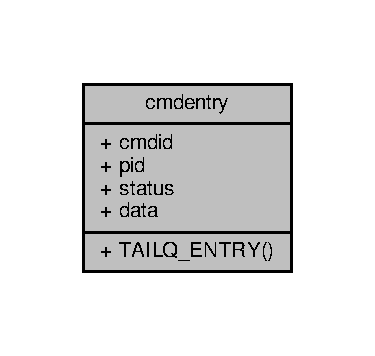
\includegraphics[width=180pt]{structcmdentry__coll__graph}
\end{center}
\end{figure}
\subsection*{Public Member Functions}
\begin{DoxyCompactItemize}
\item 
\hypertarget{structcmdentry_a7af1235a61fd7eb240cf4837647d7370}{{\bfseries T\+A\+I\+L\+Q\+\_\+\+E\+N\+T\+R\+Y} (\hyperlink{structcmdentry}{cmdentry}) entries}\label{structcmdentry_a7af1235a61fd7eb240cf4837647d7370}

\end{DoxyCompactItemize}
\subsection*{Public Attributes}
\begin{DoxyCompactItemize}
\item 
\hypertarget{structcmdentry_ab6863dee412451bf345b01ffa54c51d8}{int32\+\_\+t {\bfseries cmdid}}\label{structcmdentry_ab6863dee412451bf345b01ffa54c51d8}

\item 
\hypertarget{structcmdentry_ab1c6f5d20e481a22d8fe70906901dcd4}{pid\+\_\+t {\bfseries pid}}\label{structcmdentry_ab1c6f5d20e481a22d8fe70906901dcd4}

\item 
\hypertarget{structcmdentry_abe389e74cb293db8a0ed568594566ec8}{int {\bfseries status}}\label{structcmdentry_abe389e74cb293db8a0ed568594566ec8}

\item 
\hypertarget{structcmdentry_ae66a079b2459c358c0a2a067c2582750}{void $\ast$ {\bfseries data}}\label{structcmdentry_ae66a079b2459c358c0a2a067c2582750}

\end{DoxyCompactItemize}


The documentation for this struct was generated from the following file\+:\begin{DoxyCompactItemize}
\item 
daemon/src/vnode\+\_\+cmd.\+h\end{DoxyCompactItemize}

\hypertarget{classcore_1_1misc_1_1quagga_1_1_conf}{\section{core.\+misc.\+quagga.\+Conf Class Reference}
\label{classcore_1_1misc_1_1quagga_1_1_conf}\index{core.\+misc.\+quagga.\+Conf@{core.\+misc.\+quagga.\+Conf}}
}


Inheritance diagram for core.\+misc.\+quagga.\+Conf\+:
\nopagebreak
\begin{figure}[H]
\begin{center}
\leavevmode
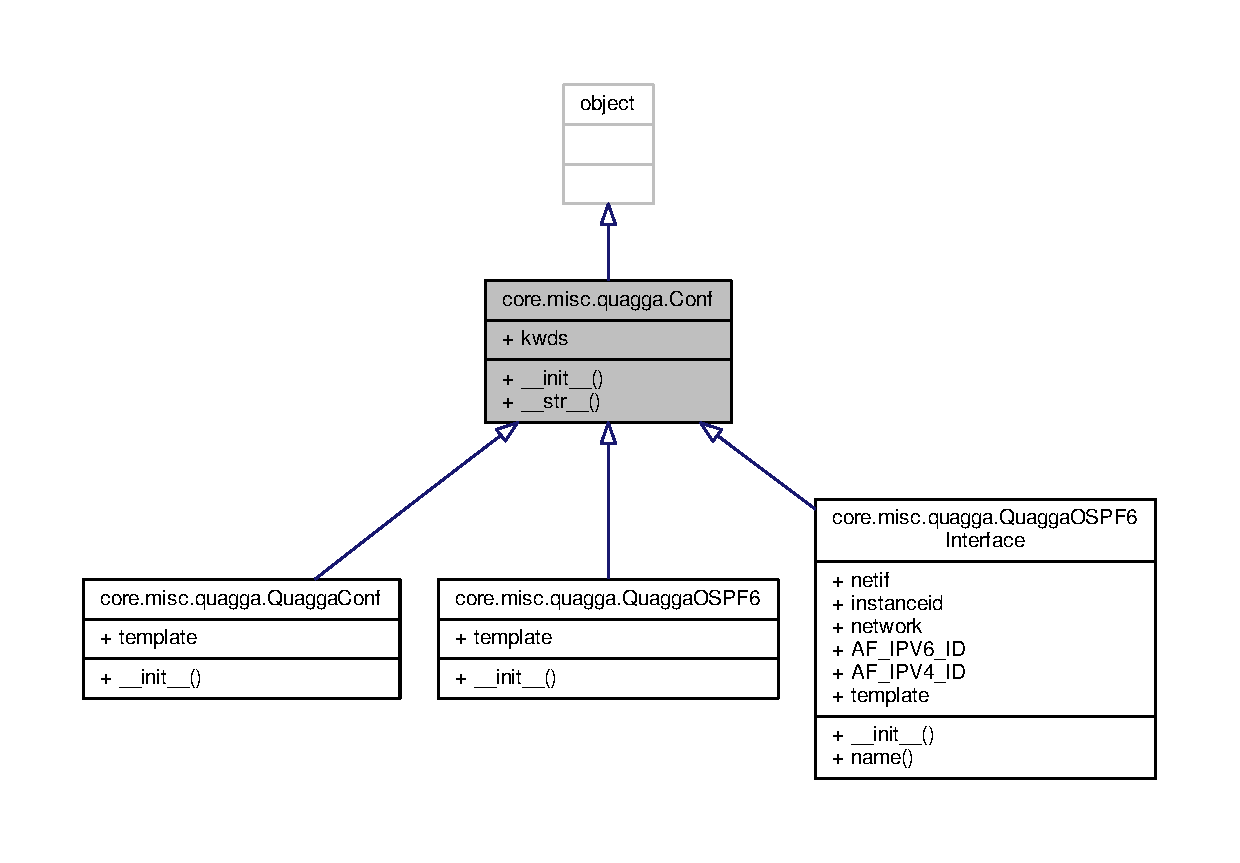
\includegraphics[width=350pt]{classcore_1_1misc_1_1quagga_1_1_conf__inherit__graph}
\end{center}
\end{figure}


Collaboration diagram for core.\+misc.\+quagga.\+Conf\+:
\nopagebreak
\begin{figure}[H]
\begin{center}
\leavevmode
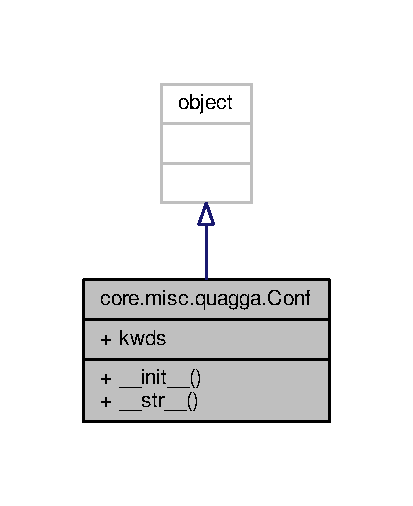
\includegraphics[width=198pt]{classcore_1_1misc_1_1quagga_1_1_conf__coll__graph}
\end{center}
\end{figure}
\subsection*{Public Member Functions}
\begin{DoxyCompactItemize}
\item 
\hypertarget{classcore_1_1misc_1_1quagga_1_1_conf_a5bdaca13872f32c6431c500514ac9158}{def {\bfseries \+\_\+\+\_\+init\+\_\+\+\_\+}}\label{classcore_1_1misc_1_1quagga_1_1_conf_a5bdaca13872f32c6431c500514ac9158}

\item 
\hypertarget{classcore_1_1misc_1_1quagga_1_1_conf_a108a8bac4a1d4fc55a4ed56956759bd3}{def {\bfseries \+\_\+\+\_\+str\+\_\+\+\_\+}}\label{classcore_1_1misc_1_1quagga_1_1_conf_a108a8bac4a1d4fc55a4ed56956759bd3}

\end{DoxyCompactItemize}
\subsection*{Public Attributes}
\begin{DoxyCompactItemize}
\item 
\hypertarget{classcore_1_1misc_1_1quagga_1_1_conf_af655c127b9417e3869b32acf9b2df0fd}{{\bfseries kwds}}\label{classcore_1_1misc_1_1quagga_1_1_conf_af655c127b9417e3869b32acf9b2df0fd}

\end{DoxyCompactItemize}


The documentation for this class was generated from the following file\+:\begin{DoxyCompactItemize}
\item 
daemon/core/misc/quagga.\+py\end{DoxyCompactItemize}

\hypertarget{classcore_1_1conf_1_1_configurable}{\section{core.\+conf.\+Configurable Class Reference}
\label{classcore_1_1conf_1_1_configurable}\index{core.\+conf.\+Configurable@{core.\+conf.\+Configurable}}
}


Inheritance diagram for core.\+conf.\+Configurable\+:
\nopagebreak
\begin{figure}[H]
\begin{center}
\leavevmode
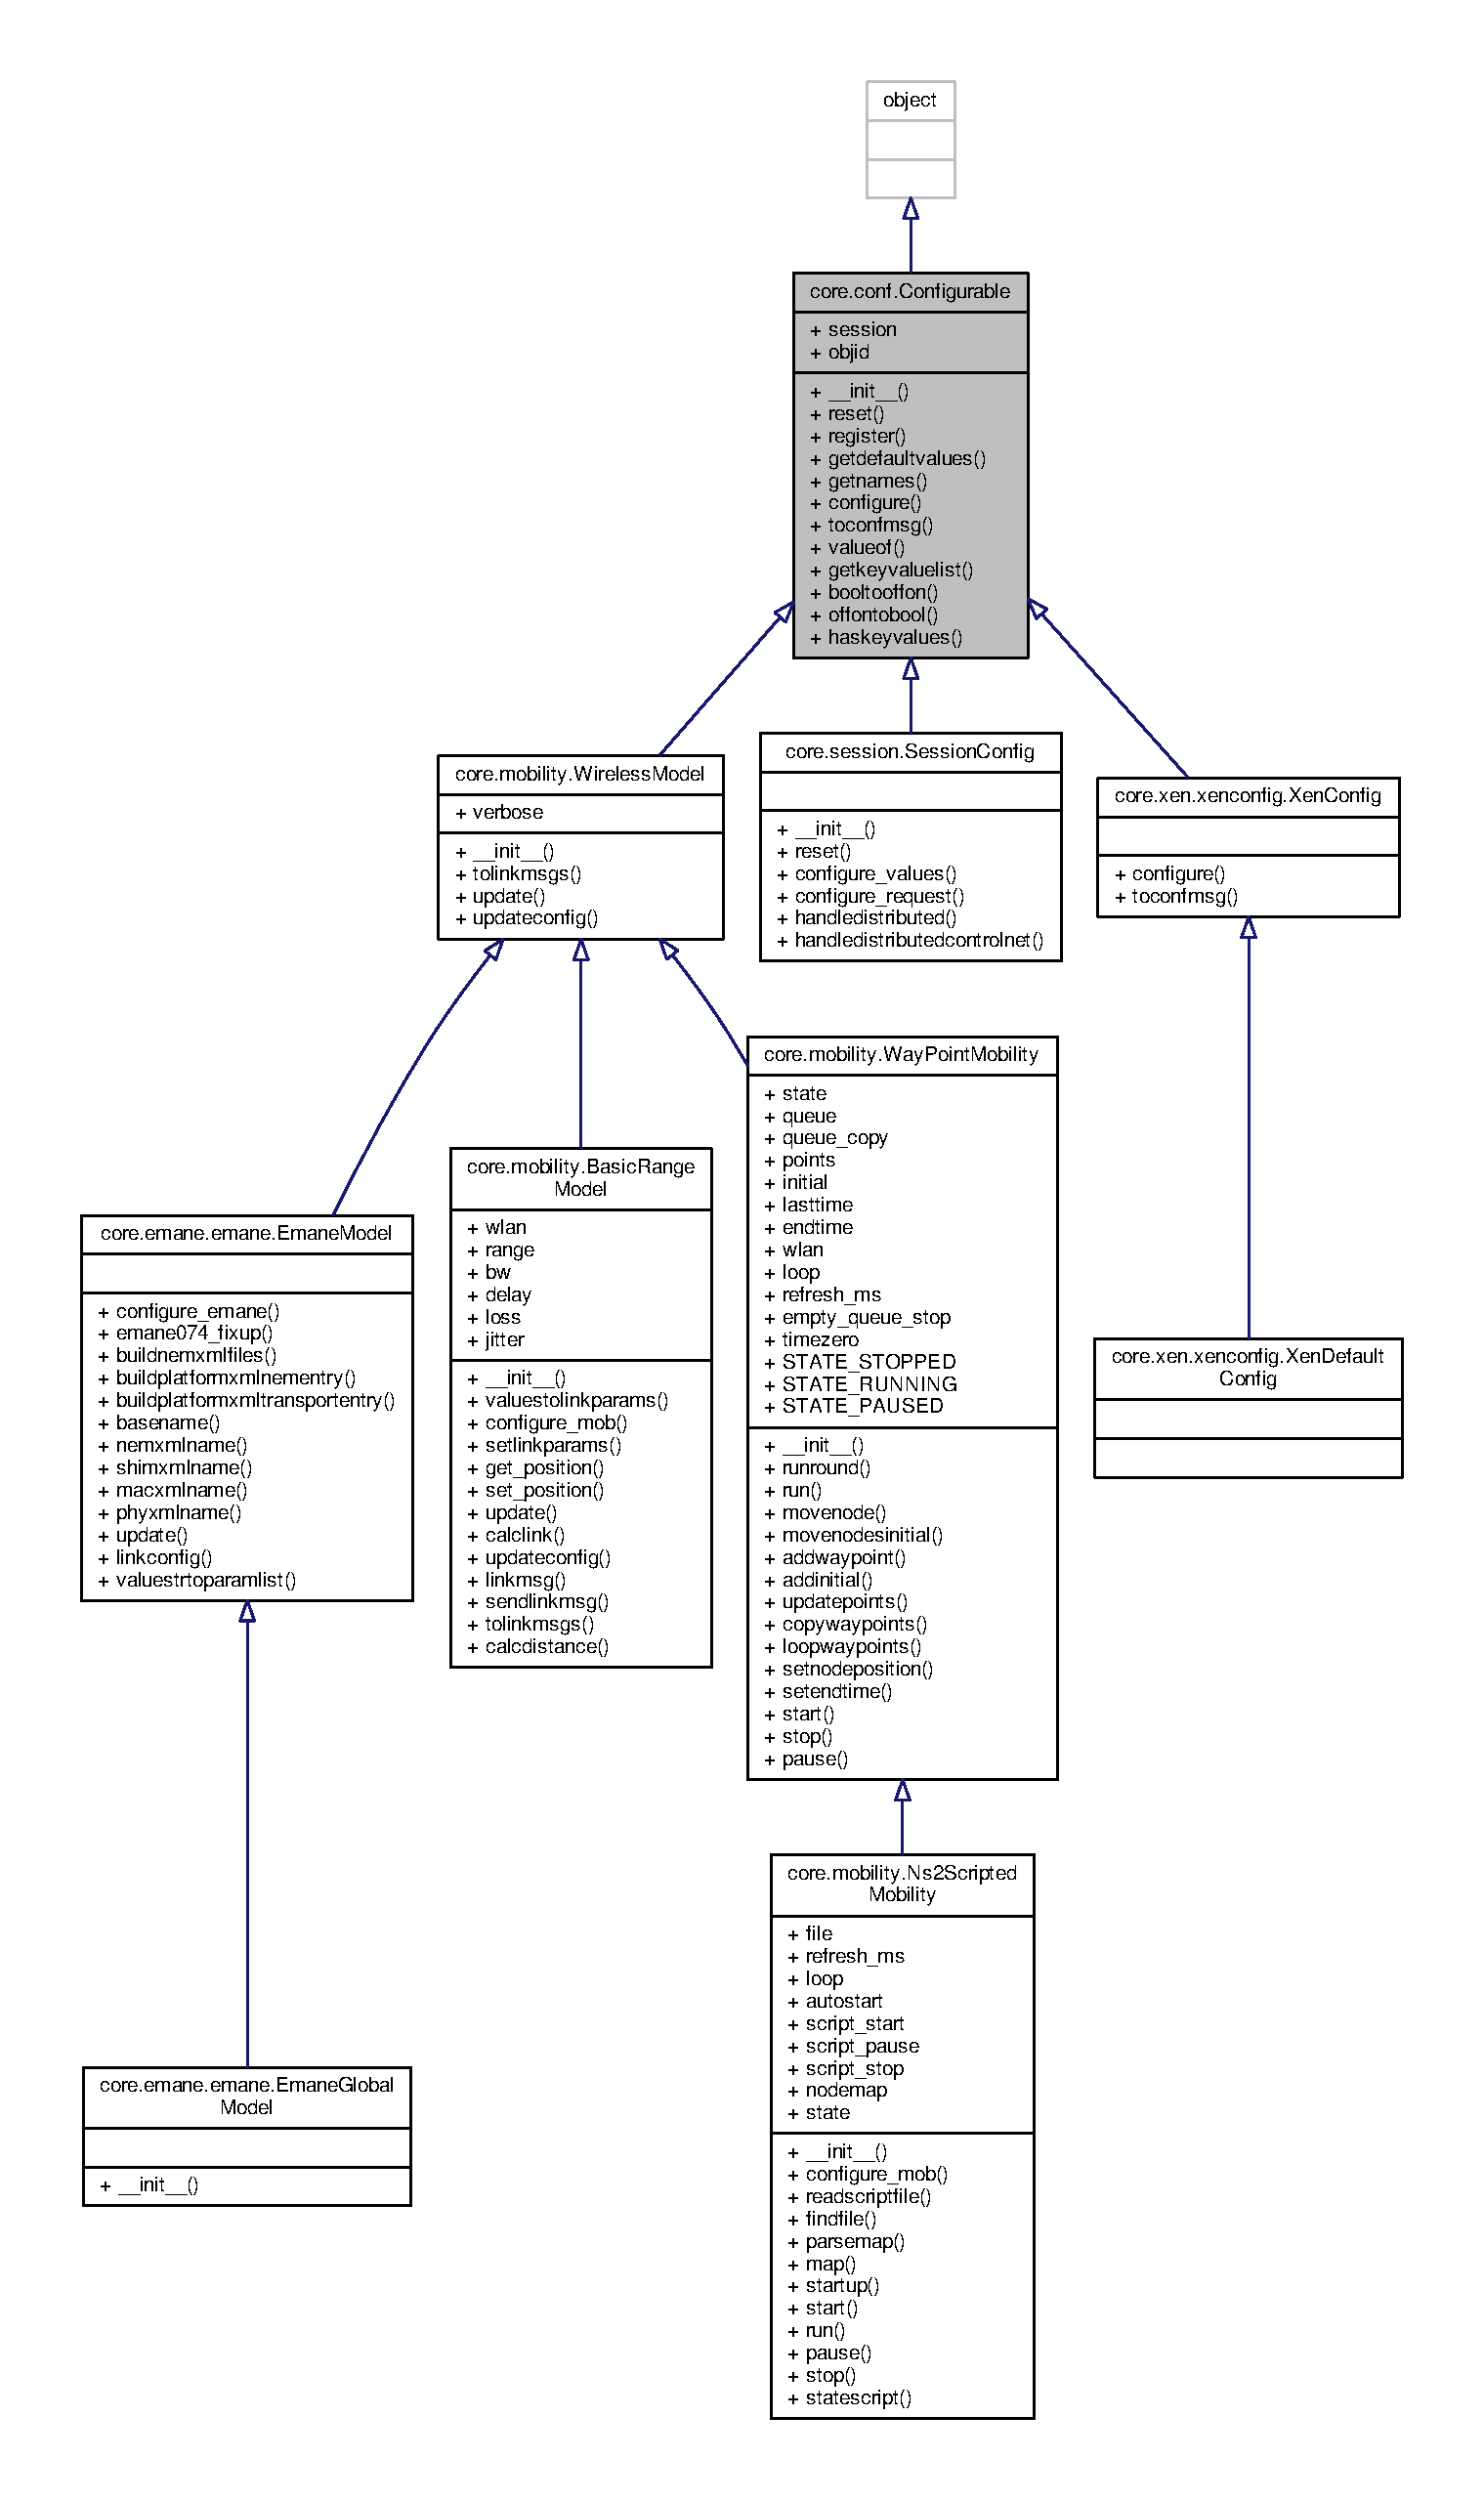
\includegraphics[height=550pt]{classcore_1_1conf_1_1_configurable__inherit__graph}
\end{center}
\end{figure}


Collaboration diagram for core.\+conf.\+Configurable\+:
\nopagebreak
\begin{figure}[H]
\begin{center}
\leavevmode
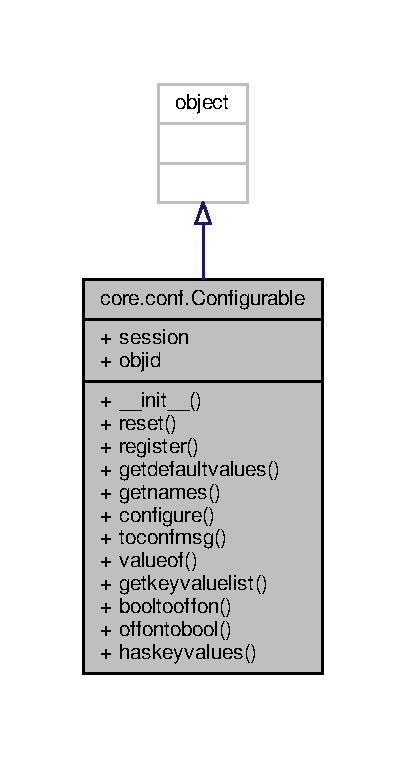
\includegraphics[width=195pt]{classcore_1_1conf_1_1_configurable__coll__graph}
\end{center}
\end{figure}
\subsection*{Public Member Functions}
\begin{DoxyCompactItemize}
\item 
\hypertarget{classcore_1_1conf_1_1_configurable_a9d5991a67c2f95656de69e3ec756f01c}{def {\bfseries \+\_\+\+\_\+init\+\_\+\+\_\+}}\label{classcore_1_1conf_1_1_configurable_a9d5991a67c2f95656de69e3ec756f01c}

\item 
\hypertarget{classcore_1_1conf_1_1_configurable_a87e5a197d1ecbd32e01eda6ea08b63ff}{def {\bfseries reset}}\label{classcore_1_1conf_1_1_configurable_a87e5a197d1ecbd32e01eda6ea08b63ff}

\item 
\hypertarget{classcore_1_1conf_1_1_configurable_af8aad484388013bb4b10494bdcbb9c33}{def {\bfseries register}}\label{classcore_1_1conf_1_1_configurable_af8aad484388013bb4b10494bdcbb9c33}

\item 
\hypertarget{classcore_1_1conf_1_1_configurable_aea0ce068624a2f390467745aff1f99d8}{def {\bfseries getdefaultvalues}}\label{classcore_1_1conf_1_1_configurable_aea0ce068624a2f390467745aff1f99d8}

\item 
\hypertarget{classcore_1_1conf_1_1_configurable_a79f79b7785137cec6e99145f07ef008c}{def {\bfseries getnames}}\label{classcore_1_1conf_1_1_configurable_a79f79b7785137cec6e99145f07ef008c}

\item 
def \hyperlink{classcore_1_1conf_1_1_configurable_a0a885b70df1d014ac5cab828020674a0}{configure}
\item 
def \hyperlink{classcore_1_1conf_1_1_configurable_afdbc51e7c337585f2533db75d5303154}{toconfmsg}
\item 
def \hyperlink{classcore_1_1conf_1_1_configurable_aeb6dbf836fb34cc0e220562a3794b7d4}{valueof}
\item 
def \hyperlink{classcore_1_1conf_1_1_configurable_a25d268d6010de8bed0795232bc51683b}{getkeyvaluelist}
\end{DoxyCompactItemize}
\subsection*{Static Public Member Functions}
\begin{DoxyCompactItemize}
\item 
def \hyperlink{classcore_1_1conf_1_1_configurable_acd09efca73c9b01512179f71a72d11a5}{booltooffon}
\item 
\hypertarget{classcore_1_1conf_1_1_configurable_a10620ed49eb196cfe332c12068ee3014}{def {\bfseries offontobool}}\label{classcore_1_1conf_1_1_configurable_a10620ed49eb196cfe332c12068ee3014}

\item 
def \hyperlink{classcore_1_1conf_1_1_configurable_a6c62bb4c659d5c9e89bc4236778aedf9}{haskeyvalues}
\end{DoxyCompactItemize}
\subsection*{Public Attributes}
\begin{DoxyCompactItemize}
\item 
\hypertarget{classcore_1_1conf_1_1_configurable_ac14f4df412110b6d0a28722371bf4ea6}{{\bfseries session}}\label{classcore_1_1conf_1_1_configurable_ac14f4df412110b6d0a28722371bf4ea6}

\item 
\hypertarget{classcore_1_1conf_1_1_configurable_af4818641eb7f672a528d3105cecdc2b0}{{\bfseries objid}}\label{classcore_1_1conf_1_1_configurable_af4818641eb7f672a528d3105cecdc2b0}

\end{DoxyCompactItemize}


\subsection{Detailed Description}
\begin{DoxyVerb}A generic class for managing configuration parameters.
    Parameters are sent via Configuration Messages, which allow the GUI
    to build dynamic dialogs depending on what is being configured.
\end{DoxyVerb}
 

\subsection{Member Function Documentation}
\hypertarget{classcore_1_1conf_1_1_configurable_acd09efca73c9b01512179f71a72d11a5}{\index{core\+::conf\+::\+Configurable@{core\+::conf\+::\+Configurable}!booltooffon@{booltooffon}}
\index{booltooffon@{booltooffon}!core\+::conf\+::\+Configurable@{core\+::conf\+::\+Configurable}}
\subsubsection[{booltooffon}]{\setlength{\rightskip}{0pt plus 5cm}def core.\+conf.\+Configurable.\+booltooffon (
\begin{DoxyParamCaption}
\item[{}]{value}
\end{DoxyParamCaption}
)\hspace{0.3cm}{\ttfamily [static]}}}\label{classcore_1_1conf_1_1_configurable_acd09efca73c9b01512179f71a72d11a5}
\begin{DoxyVerb}Convenience helper turns bool into on (True) or off (False) string.
\end{DoxyVerb}
 \hypertarget{classcore_1_1conf_1_1_configurable_a0a885b70df1d014ac5cab828020674a0}{\index{core\+::conf\+::\+Configurable@{core\+::conf\+::\+Configurable}!configure@{configure}}
\index{configure@{configure}!core\+::conf\+::\+Configurable@{core\+::conf\+::\+Configurable}}
\subsubsection[{configure}]{\setlength{\rightskip}{0pt plus 5cm}def core.\+conf.\+Configurable.\+configure (
\begin{DoxyParamCaption}
\item[{}]{cls, }
\item[{}]{mgr, }
\item[{}]{msg}
\end{DoxyParamCaption}
)}}\label{classcore_1_1conf_1_1_configurable_a0a885b70df1d014ac5cab828020674a0}
\begin{DoxyVerb}Handle configuration messages for this object.
\end{DoxyVerb}
 \hypertarget{classcore_1_1conf_1_1_configurable_a25d268d6010de8bed0795232bc51683b}{\index{core\+::conf\+::\+Configurable@{core\+::conf\+::\+Configurable}!getkeyvaluelist@{getkeyvaluelist}}
\index{getkeyvaluelist@{getkeyvaluelist}!core\+::conf\+::\+Configurable@{core\+::conf\+::\+Configurable}}
\subsubsection[{getkeyvaluelist}]{\setlength{\rightskip}{0pt plus 5cm}def core.\+conf.\+Configurable.\+getkeyvaluelist (
\begin{DoxyParamCaption}
\item[{}]{self}
\end{DoxyParamCaption}
)}}\label{classcore_1_1conf_1_1_configurable_a25d268d6010de8bed0795232bc51683b}
\begin{DoxyVerb}Helper to return a list of (key, value) tuples. Keys come from
self._confmatrix and values are instance attributes.
\end{DoxyVerb}
 \hypertarget{classcore_1_1conf_1_1_configurable_a6c62bb4c659d5c9e89bc4236778aedf9}{\index{core\+::conf\+::\+Configurable@{core\+::conf\+::\+Configurable}!haskeyvalues@{haskeyvalues}}
\index{haskeyvalues@{haskeyvalues}!core\+::conf\+::\+Configurable@{core\+::conf\+::\+Configurable}}
\subsubsection[{haskeyvalues}]{\setlength{\rightskip}{0pt plus 5cm}def core.\+conf.\+Configurable.\+haskeyvalues (
\begin{DoxyParamCaption}
\item[{}]{values}
\end{DoxyParamCaption}
)\hspace{0.3cm}{\ttfamily [static]}}}\label{classcore_1_1conf_1_1_configurable_a6c62bb4c659d5c9e89bc4236778aedf9}
\begin{DoxyVerb}Helper to check for list of key=value pairs versus a plain old
    list of values. Returns True if all elements are "key=value".
\end{DoxyVerb}
 \hypertarget{classcore_1_1conf_1_1_configurable_afdbc51e7c337585f2533db75d5303154}{\index{core\+::conf\+::\+Configurable@{core\+::conf\+::\+Configurable}!toconfmsg@{toconfmsg}}
\index{toconfmsg@{toconfmsg}!core\+::conf\+::\+Configurable@{core\+::conf\+::\+Configurable}}
\subsubsection[{toconfmsg}]{\setlength{\rightskip}{0pt plus 5cm}def core.\+conf.\+Configurable.\+toconfmsg (
\begin{DoxyParamCaption}
\item[{}]{cls, }
\item[{}]{flags, }
\item[{}]{nodenum, }
\item[{}]{typeflags, }
\item[{}]{values}
\end{DoxyParamCaption}
)}}\label{classcore_1_1conf_1_1_configurable_afdbc51e7c337585f2533db75d5303154}
\begin{DoxyVerb}Convert this class to a Config API message. Some TLVs are defined
    by the class, but node number, conf type flags, and values must
    be passed in.
\end{DoxyVerb}
 \hypertarget{classcore_1_1conf_1_1_configurable_aeb6dbf836fb34cc0e220562a3794b7d4}{\index{core\+::conf\+::\+Configurable@{core\+::conf\+::\+Configurable}!valueof@{valueof}}
\index{valueof@{valueof}!core\+::conf\+::\+Configurable@{core\+::conf\+::\+Configurable}}
\subsubsection[{valueof}]{\setlength{\rightskip}{0pt plus 5cm}def core.\+conf.\+Configurable.\+valueof (
\begin{DoxyParamCaption}
\item[{}]{cls, }
\item[{}]{name, }
\item[{}]{values}
\end{DoxyParamCaption}
)}}\label{classcore_1_1conf_1_1_configurable_aeb6dbf836fb34cc0e220562a3794b7d4}
\begin{DoxyVerb}Helper to return a value by the name defined in confmatrix.
    Checks if it is boolean\end{DoxyVerb}
 

The documentation for this class was generated from the following file\+:\begin{DoxyCompactItemize}
\item 
daemon/core/conf.\+py\end{DoxyCompactItemize}

\hypertarget{classcore_1_1conf_1_1_configurable_manager}{\section{core.\+conf.\+Configurable\+Manager Class Reference}
\label{classcore_1_1conf_1_1_configurable_manager}\index{core.\+conf.\+Configurable\+Manager@{core.\+conf.\+Configurable\+Manager}}
}


Inheritance diagram for core.\+conf.\+Configurable\+Manager\+:
\nopagebreak
\begin{figure}[H]
\begin{center}
\leavevmode
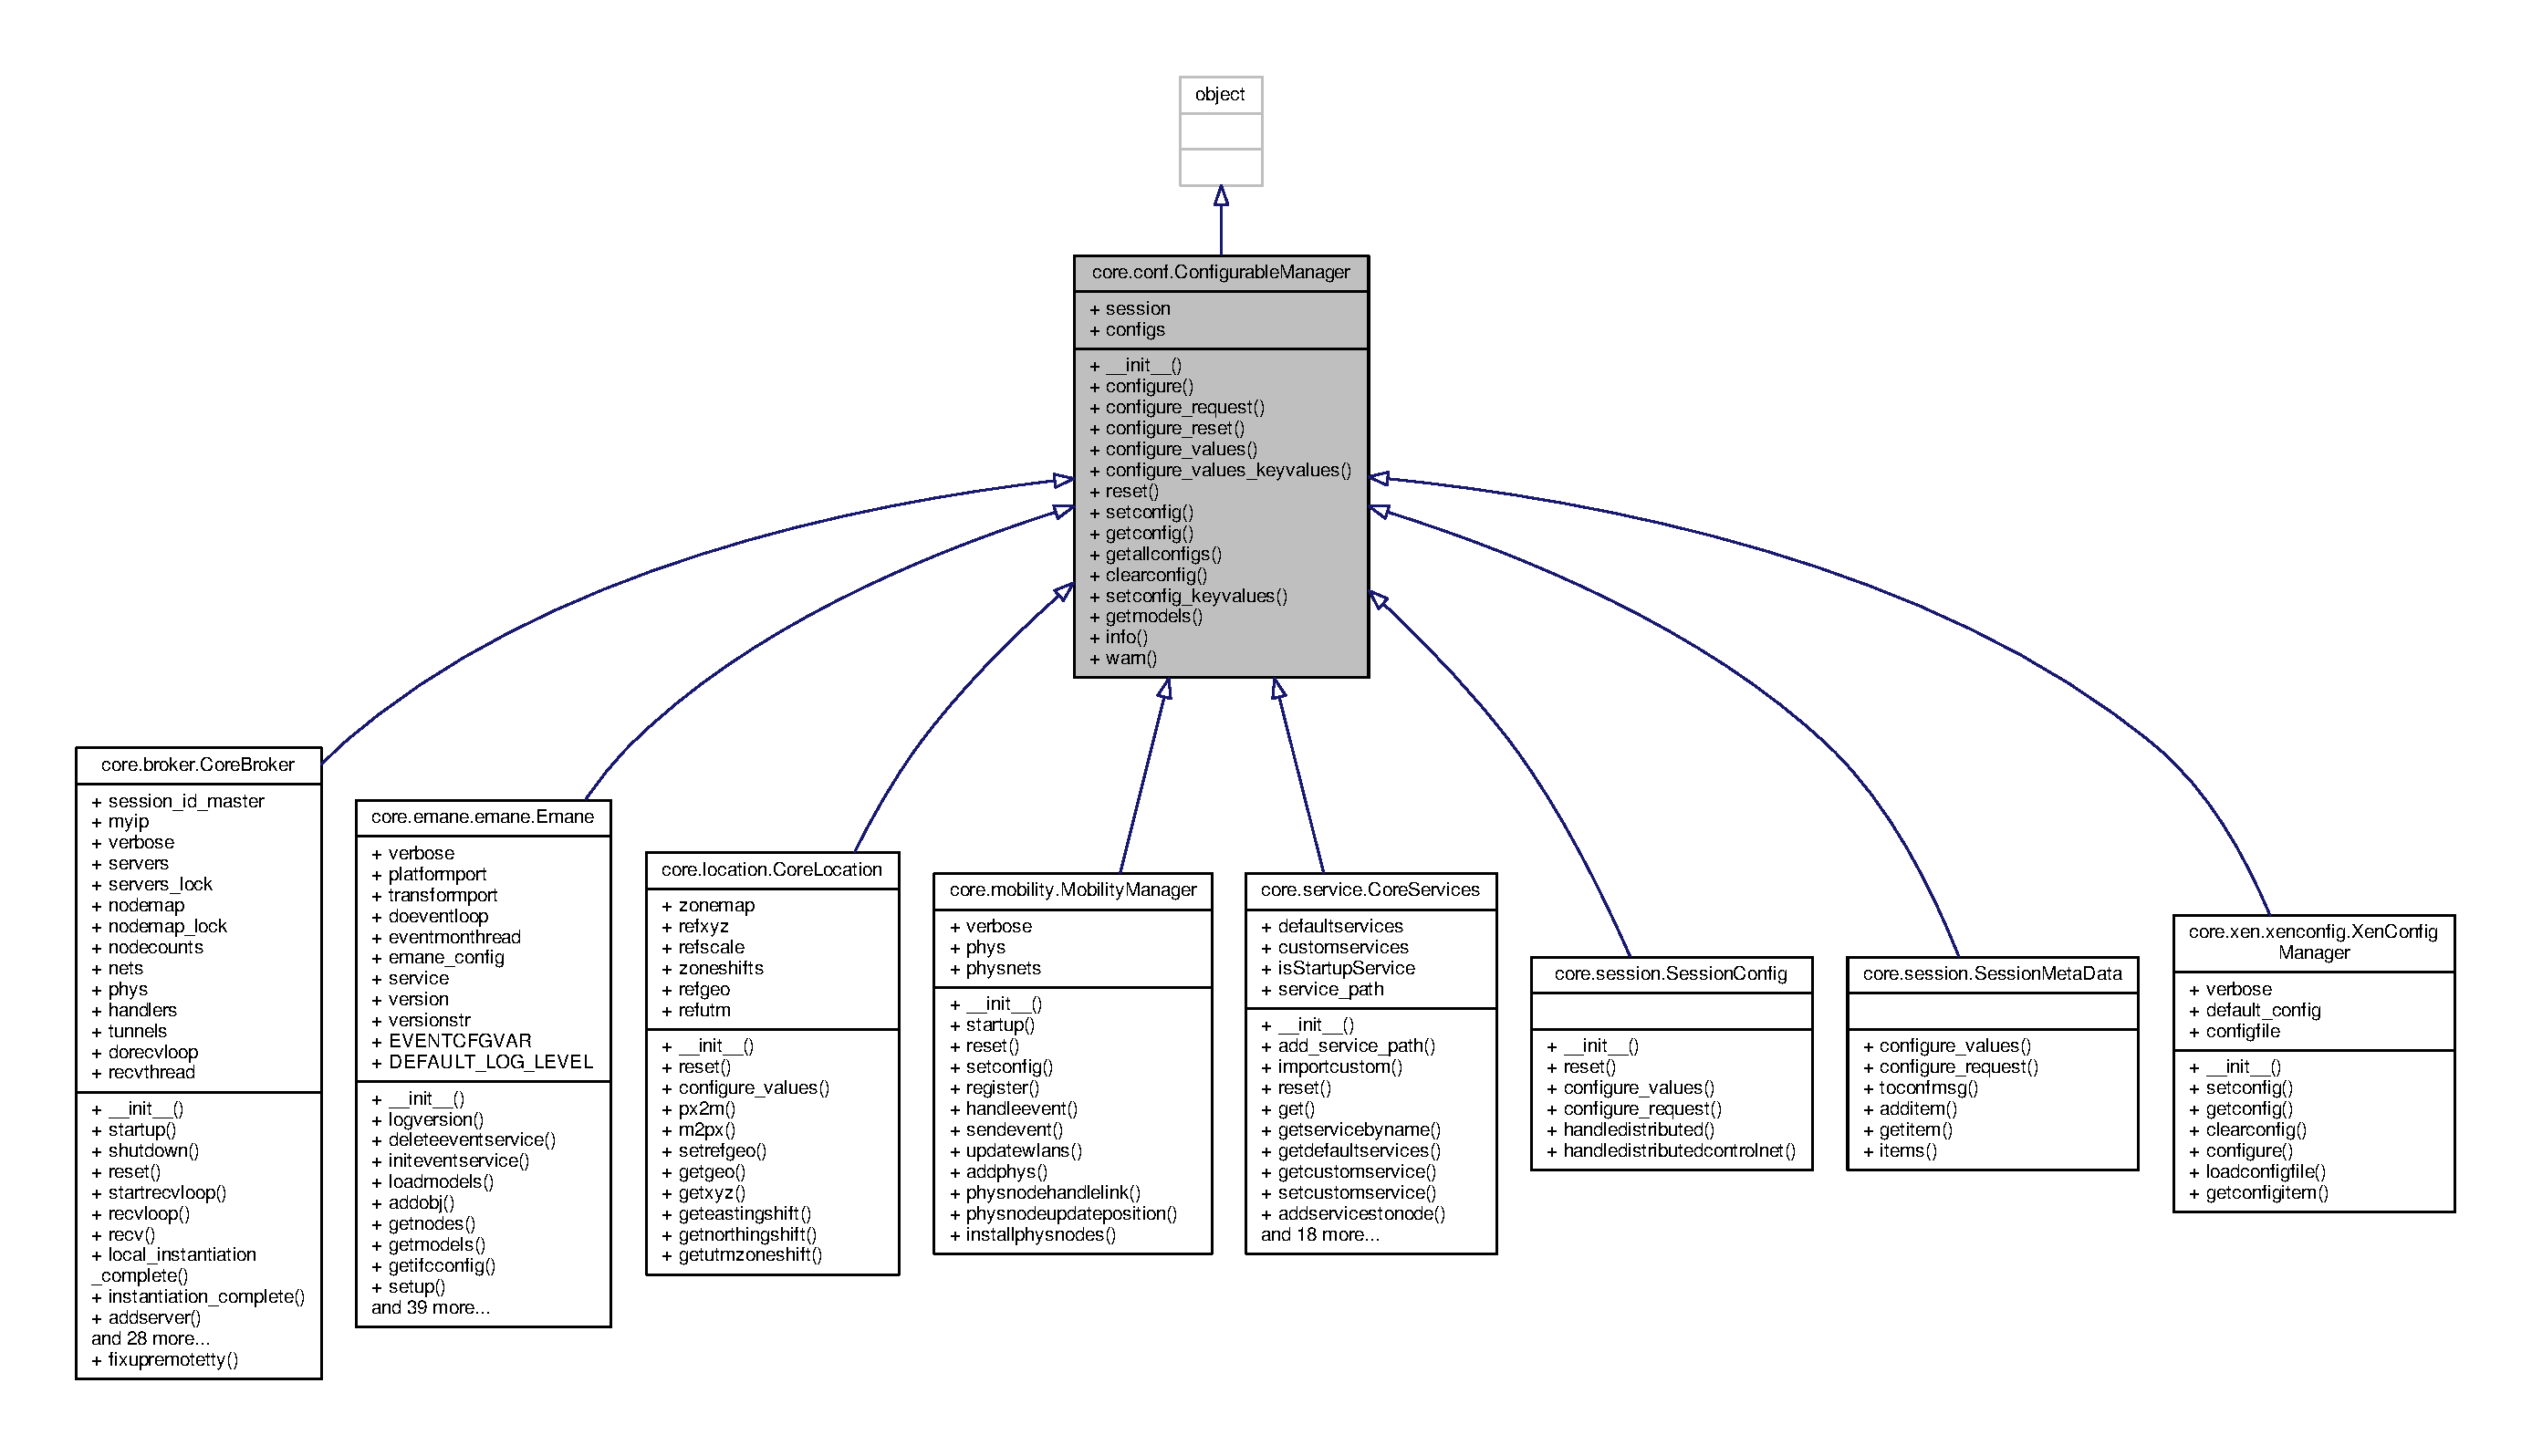
\includegraphics[width=350pt]{classcore_1_1conf_1_1_configurable_manager__inherit__graph}
\end{center}
\end{figure}


Collaboration diagram for core.\+conf.\+Configurable\+Manager\+:
\nopagebreak
\begin{figure}[H]
\begin{center}
\leavevmode
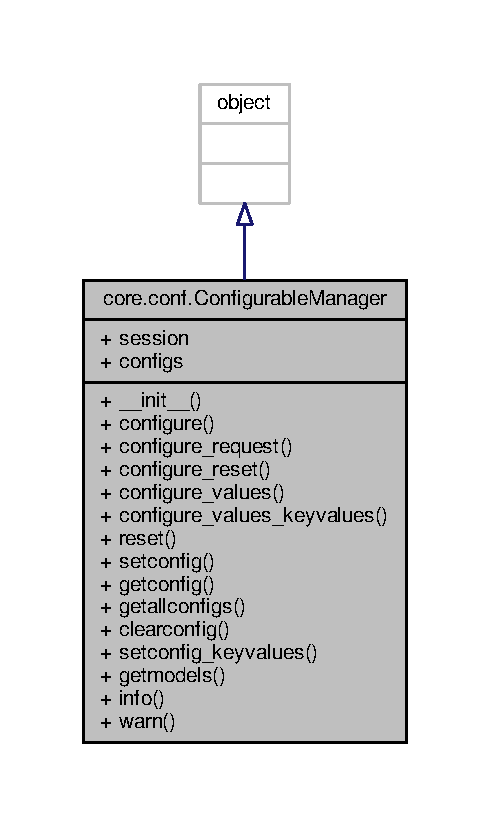
\includegraphics[width=235pt]{classcore_1_1conf_1_1_configurable_manager__coll__graph}
\end{center}
\end{figure}
\subsection*{Public Member Functions}
\begin{DoxyCompactItemize}
\item 
\hypertarget{classcore_1_1conf_1_1_configurable_manager_a199933aed21d63d5a45963dedde363b8}{def {\bfseries \+\_\+\+\_\+init\+\_\+\+\_\+}}\label{classcore_1_1conf_1_1_configurable_manager_a199933aed21d63d5a45963dedde363b8}

\item 
def \hyperlink{classcore_1_1conf_1_1_configurable_manager_a323cd80662589456e92446bc00d3f121}{configure}
\item 
def \hyperlink{classcore_1_1conf_1_1_configurable_manager_a61f4ce61e2e9071044ad9cdb5b62c5d8}{configure\+\_\+request}
\item 
def \hyperlink{classcore_1_1conf_1_1_configurable_manager_a7bf7ec34d9577b402caf567116adadb0}{configure\+\_\+reset}
\item 
def \hyperlink{classcore_1_1conf_1_1_configurable_manager_ada87a29998b14563fe9f1b92a9d5cd5f}{configure\+\_\+values}
\item 
def \hyperlink{classcore_1_1conf_1_1_configurable_manager_ab1de29d30306eabba9805c8f39f1806c}{configure\+\_\+values\+\_\+keyvalues}
\item 
\hypertarget{classcore_1_1conf_1_1_configurable_manager_ab3d219018ffdf814972b79cf613dddc1}{def {\bfseries reset}}\label{classcore_1_1conf_1_1_configurable_manager_ab3d219018ffdf814972b79cf613dddc1}

\item 
def \hyperlink{classcore_1_1conf_1_1_configurable_manager_a4594891c10805361b6c96e6dfbf742da}{setconfig}
\item 
def \hyperlink{classcore_1_1conf_1_1_configurable_manager_a50e76fc0629141783acc1560e8ff8d6b}{getconfig}
\item 
def \hyperlink{classcore_1_1conf_1_1_configurable_manager_a38c5d075bc02ba0d9aa5bd9752f11c16}{getallconfigs}
\item 
def \hyperlink{classcore_1_1conf_1_1_configurable_manager_a8cc2f85aaad6cc0c9f04469c3554d320}{clearconfig}
\item 
def \hyperlink{classcore_1_1conf_1_1_configurable_manager_adb9d5645b6551d5928392cacfe116961}{setconfig\+\_\+keyvalues}
\item 
def \hyperlink{classcore_1_1conf_1_1_configurable_manager_aa37e907c84352572c5d080f2b27385d5}{getmodels}
\item 
\hypertarget{classcore_1_1conf_1_1_configurable_manager_a914e3d2cd2ca6c4ad0eaa149505bb38f}{def {\bfseries info}}\label{classcore_1_1conf_1_1_configurable_manager_a914e3d2cd2ca6c4ad0eaa149505bb38f}

\item 
\hypertarget{classcore_1_1conf_1_1_configurable_manager_ad815521e7aa4379a19c5973ce2cc58cb}{def {\bfseries warn}}\label{classcore_1_1conf_1_1_configurable_manager_ad815521e7aa4379a19c5973ce2cc58cb}

\end{DoxyCompactItemize}
\subsection*{Public Attributes}
\begin{DoxyCompactItemize}
\item 
\hypertarget{classcore_1_1conf_1_1_configurable_manager_a2cabf2cc60e378c338c0ea6869e6b341}{{\bfseries session}}\label{classcore_1_1conf_1_1_configurable_manager_a2cabf2cc60e378c338c0ea6869e6b341}

\item 
\hypertarget{classcore_1_1conf_1_1_configurable_manager_ad43a165b5d90b8a134b4b13453f5fd57}{{\bfseries configs}}\label{classcore_1_1conf_1_1_configurable_manager_ad43a165b5d90b8a134b4b13453f5fd57}

\end{DoxyCompactItemize}


\subsection{Detailed Description}
\begin{DoxyVerb}A generic class for managing Configurables. This class can register
    with a session to receive Config Messages for setting some parameters
    for itself or for the Configurables that it manages.
\end{DoxyVerb}
 

\subsection{Member Function Documentation}
\hypertarget{classcore_1_1conf_1_1_configurable_manager_a8cc2f85aaad6cc0c9f04469c3554d320}{\index{core\+::conf\+::\+Configurable\+Manager@{core\+::conf\+::\+Configurable\+Manager}!clearconfig@{clearconfig}}
\index{clearconfig@{clearconfig}!core\+::conf\+::\+Configurable\+Manager@{core\+::conf\+::\+Configurable\+Manager}}
\subsubsection[{clearconfig}]{\setlength{\rightskip}{0pt plus 5cm}def core.\+conf.\+Configurable\+Manager.\+clearconfig (
\begin{DoxyParamCaption}
\item[{}]{self, }
\item[{}]{nodenum}
\end{DoxyParamCaption}
)}}\label{classcore_1_1conf_1_1_configurable_manager_a8cc2f85aaad6cc0c9f04469c3554d320}
\begin{DoxyVerb}remove configuration values for the specified node;
    when nodenum is None, remove all configuration values 
\end{DoxyVerb}
 \hypertarget{classcore_1_1conf_1_1_configurable_manager_a323cd80662589456e92446bc00d3f121}{\index{core\+::conf\+::\+Configurable\+Manager@{core\+::conf\+::\+Configurable\+Manager}!configure@{configure}}
\index{configure@{configure}!core\+::conf\+::\+Configurable\+Manager@{core\+::conf\+::\+Configurable\+Manager}}
\subsubsection[{configure}]{\setlength{\rightskip}{0pt plus 5cm}def core.\+conf.\+Configurable\+Manager.\+configure (
\begin{DoxyParamCaption}
\item[{}]{self, }
\item[{}]{session, }
\item[{}]{msg}
\end{DoxyParamCaption}
)}}\label{classcore_1_1conf_1_1_configurable_manager_a323cd80662589456e92446bc00d3f121}
\begin{DoxyVerb}Handle configure messages. The configuration message sent to a
    ConfigurableManager usually is used to:
    1. Request a list of Configurables (request flag)
    2. Reset manager and clear configs (reset flag)
    3. Send values that configure the manager or one of its 
       Configurables
       
    Returns any reply messages.
\end{DoxyVerb}
 \hypertarget{classcore_1_1conf_1_1_configurable_manager_a61f4ce61e2e9071044ad9cdb5b62c5d8}{\index{core\+::conf\+::\+Configurable\+Manager@{core\+::conf\+::\+Configurable\+Manager}!configure\+\_\+request@{configure\+\_\+request}}
\index{configure\+\_\+request@{configure\+\_\+request}!core\+::conf\+::\+Configurable\+Manager@{core\+::conf\+::\+Configurable\+Manager}}
\subsubsection[{configure\+\_\+request}]{\setlength{\rightskip}{0pt plus 5cm}def core.\+conf.\+Configurable\+Manager.\+configure\+\_\+request (
\begin{DoxyParamCaption}
\item[{}]{self, }
\item[{}]{msg}
\end{DoxyParamCaption}
)}}\label{classcore_1_1conf_1_1_configurable_manager_a61f4ce61e2e9071044ad9cdb5b62c5d8}
\begin{DoxyVerb}Request configuration data.
\end{DoxyVerb}
 \hypertarget{classcore_1_1conf_1_1_configurable_manager_a7bf7ec34d9577b402caf567116adadb0}{\index{core\+::conf\+::\+Configurable\+Manager@{core\+::conf\+::\+Configurable\+Manager}!configure\+\_\+reset@{configure\+\_\+reset}}
\index{configure\+\_\+reset@{configure\+\_\+reset}!core\+::conf\+::\+Configurable\+Manager@{core\+::conf\+::\+Configurable\+Manager}}
\subsubsection[{configure\+\_\+reset}]{\setlength{\rightskip}{0pt plus 5cm}def core.\+conf.\+Configurable\+Manager.\+configure\+\_\+reset (
\begin{DoxyParamCaption}
\item[{}]{self, }
\item[{}]{msg}
\end{DoxyParamCaption}
)}}\label{classcore_1_1conf_1_1_configurable_manager_a7bf7ec34d9577b402caf567116adadb0}
\begin{DoxyVerb}By default, resets this manager to clear configs.
\end{DoxyVerb}
 \hypertarget{classcore_1_1conf_1_1_configurable_manager_ada87a29998b14563fe9f1b92a9d5cd5f}{\index{core\+::conf\+::\+Configurable\+Manager@{core\+::conf\+::\+Configurable\+Manager}!configure\+\_\+values@{configure\+\_\+values}}
\index{configure\+\_\+values@{configure\+\_\+values}!core\+::conf\+::\+Configurable\+Manager@{core\+::conf\+::\+Configurable\+Manager}}
\subsubsection[{configure\+\_\+values}]{\setlength{\rightskip}{0pt plus 5cm}def core.\+conf.\+Configurable\+Manager.\+configure\+\_\+values (
\begin{DoxyParamCaption}
\item[{}]{self, }
\item[{}]{msg, }
\item[{}]{values}
\end{DoxyParamCaption}
)}}\label{classcore_1_1conf_1_1_configurable_manager_ada87a29998b14563fe9f1b92a9d5cd5f}
\begin{DoxyVerb}Values have been sent to this manager.
\end{DoxyVerb}
 \hypertarget{classcore_1_1conf_1_1_configurable_manager_ab1de29d30306eabba9805c8f39f1806c}{\index{core\+::conf\+::\+Configurable\+Manager@{core\+::conf\+::\+Configurable\+Manager}!configure\+\_\+values\+\_\+keyvalues@{configure\+\_\+values\+\_\+keyvalues}}
\index{configure\+\_\+values\+\_\+keyvalues@{configure\+\_\+values\+\_\+keyvalues}!core\+::conf\+::\+Configurable\+Manager@{core\+::conf\+::\+Configurable\+Manager}}
\subsubsection[{configure\+\_\+values\+\_\+keyvalues}]{\setlength{\rightskip}{0pt plus 5cm}def core.\+conf.\+Configurable\+Manager.\+configure\+\_\+values\+\_\+keyvalues (
\begin{DoxyParamCaption}
\item[{}]{self, }
\item[{}]{msg, }
\item[{}]{values, }
\item[{}]{target, }
\item[{}]{keys}
\end{DoxyParamCaption}
)}}\label{classcore_1_1conf_1_1_configurable_manager_ab1de29d30306eabba9805c8f39f1806c}
\begin{DoxyVerb}Helper that can be used for configure_values for parsing in
    'key=value' strings from a values field. The key name must be
    in the keys list, and target.key=value is set.
\end{DoxyVerb}
 \hypertarget{classcore_1_1conf_1_1_configurable_manager_a38c5d075bc02ba0d9aa5bd9752f11c16}{\index{core\+::conf\+::\+Configurable\+Manager@{core\+::conf\+::\+Configurable\+Manager}!getallconfigs@{getallconfigs}}
\index{getallconfigs@{getallconfigs}!core\+::conf\+::\+Configurable\+Manager@{core\+::conf\+::\+Configurable\+Manager}}
\subsubsection[{getallconfigs}]{\setlength{\rightskip}{0pt plus 5cm}def core.\+conf.\+Configurable\+Manager.\+getallconfigs (
\begin{DoxyParamCaption}
\item[{}]{self, }
\item[{}]{use\+\_\+clsmap = {\ttfamily True}}
\end{DoxyParamCaption}
)}}\label{classcore_1_1conf_1_1_configurable_manager_a38c5d075bc02ba0d9aa5bd9752f11c16}
\begin{DoxyVerb}Return (nodenum, conftype, values) tuples for all stored configs.
Used when reconnecting to a session.
\end{DoxyVerb}
 \hypertarget{classcore_1_1conf_1_1_configurable_manager_a50e76fc0629141783acc1560e8ff8d6b}{\index{core\+::conf\+::\+Configurable\+Manager@{core\+::conf\+::\+Configurable\+Manager}!getconfig@{getconfig}}
\index{getconfig@{getconfig}!core\+::conf\+::\+Configurable\+Manager@{core\+::conf\+::\+Configurable\+Manager}}
\subsubsection[{getconfig}]{\setlength{\rightskip}{0pt plus 5cm}def core.\+conf.\+Configurable\+Manager.\+getconfig (
\begin{DoxyParamCaption}
\item[{}]{self, }
\item[{}]{nodenum, }
\item[{}]{conftype, }
\item[{}]{defaultvalues}
\end{DoxyParamCaption}
)}}\label{classcore_1_1conf_1_1_configurable_manager_a50e76fc0629141783acc1560e8ff8d6b}
\begin{DoxyVerb}get configuration values for a node; if the values don't exist in
    our dictionary then return the default values supplied
\end{DoxyVerb}
 \hypertarget{classcore_1_1conf_1_1_configurable_manager_aa37e907c84352572c5d080f2b27385d5}{\index{core\+::conf\+::\+Configurable\+Manager@{core\+::conf\+::\+Configurable\+Manager}!getmodels@{getmodels}}
\index{getmodels@{getmodels}!core\+::conf\+::\+Configurable\+Manager@{core\+::conf\+::\+Configurable\+Manager}}
\subsubsection[{getmodels}]{\setlength{\rightskip}{0pt plus 5cm}def core.\+conf.\+Configurable\+Manager.\+getmodels (
\begin{DoxyParamCaption}
\item[{}]{self, }
\item[{}]{n}
\end{DoxyParamCaption}
)}}\label{classcore_1_1conf_1_1_configurable_manager_aa37e907c84352572c5d080f2b27385d5}
\begin{DoxyVerb}Return a list of model classes and values for a net if one has been
configured. This is invoked when exporting a session to XML.
This assumes self.configs contains an iterable of (model-names, values)
and a self._modelclsmapdict exists.
\end{DoxyVerb}
 \hypertarget{classcore_1_1conf_1_1_configurable_manager_a4594891c10805361b6c96e6dfbf742da}{\index{core\+::conf\+::\+Configurable\+Manager@{core\+::conf\+::\+Configurable\+Manager}!setconfig@{setconfig}}
\index{setconfig@{setconfig}!core\+::conf\+::\+Configurable\+Manager@{core\+::conf\+::\+Configurable\+Manager}}
\subsubsection[{setconfig}]{\setlength{\rightskip}{0pt plus 5cm}def core.\+conf.\+Configurable\+Manager.\+setconfig (
\begin{DoxyParamCaption}
\item[{}]{self, }
\item[{}]{nodenum, }
\item[{}]{conftype, }
\item[{}]{values}
\end{DoxyParamCaption}
)}}\label{classcore_1_1conf_1_1_configurable_manager_a4594891c10805361b6c96e6dfbf742da}
\begin{DoxyVerb}add configuration values for a node to a dictionary; values are
    usually received from a Configuration Message, and may refer to a
    node for which no object exists yet
\end{DoxyVerb}
 \hypertarget{classcore_1_1conf_1_1_configurable_manager_adb9d5645b6551d5928392cacfe116961}{\index{core\+::conf\+::\+Configurable\+Manager@{core\+::conf\+::\+Configurable\+Manager}!setconfig\+\_\+keyvalues@{setconfig\+\_\+keyvalues}}
\index{setconfig\+\_\+keyvalues@{setconfig\+\_\+keyvalues}!core\+::conf\+::\+Configurable\+Manager@{core\+::conf\+::\+Configurable\+Manager}}
\subsubsection[{setconfig\+\_\+keyvalues}]{\setlength{\rightskip}{0pt plus 5cm}def core.\+conf.\+Configurable\+Manager.\+setconfig\+\_\+keyvalues (
\begin{DoxyParamCaption}
\item[{}]{self, }
\item[{}]{nodenum, }
\item[{}]{conftype, }
\item[{}]{keyvalues}
\end{DoxyParamCaption}
)}}\label{classcore_1_1conf_1_1_configurable_manager_adb9d5645b6551d5928392cacfe116961}
\begin{DoxyVerb}keyvalues list of tuples
\end{DoxyVerb}
 

The documentation for this class was generated from the following file\+:\begin{DoxyCompactItemize}
\item 
daemon/core/conf.\+py\end{DoxyCompactItemize}

\hypertarget{classcore_1_1coreserver_1_1_core_aux_server}{\section{core.\+coreserver.\+Core\+Aux\+Server Class Reference}
\label{classcore_1_1coreserver_1_1_core_aux_server}\index{core.\+coreserver.\+Core\+Aux\+Server@{core.\+coreserver.\+Core\+Aux\+Server}}
}


Inheritance diagram for core.\+coreserver.\+Core\+Aux\+Server\+:
\nopagebreak
\begin{figure}[H]
\begin{center}
\leavevmode
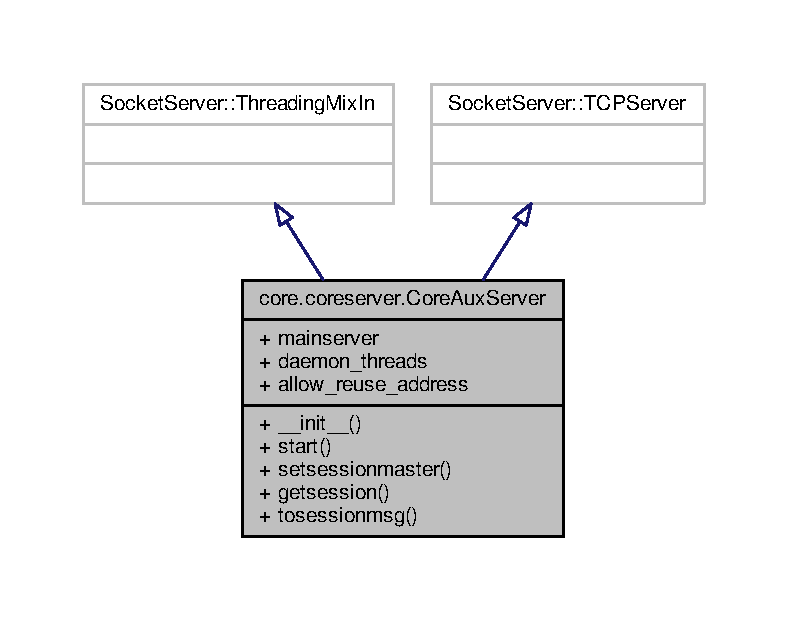
\includegraphics[width=350pt]{classcore_1_1coreserver_1_1_core_aux_server__inherit__graph}
\end{center}
\end{figure}


Collaboration diagram for core.\+coreserver.\+Core\+Aux\+Server\+:
\nopagebreak
\begin{figure}[H]
\begin{center}
\leavevmode
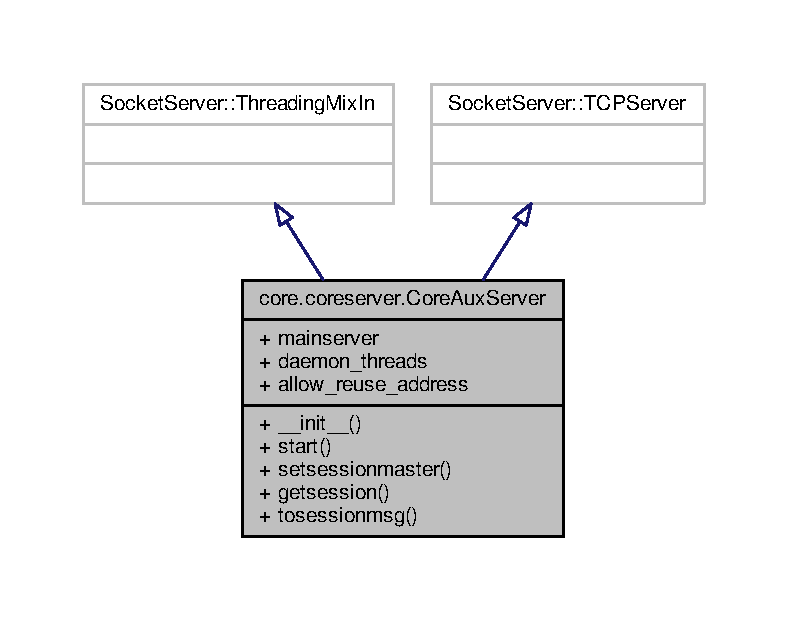
\includegraphics[width=350pt]{classcore_1_1coreserver_1_1_core_aux_server__coll__graph}
\end{center}
\end{figure}
\subsection*{Public Member Functions}
\begin{DoxyCompactItemize}
\item 
\hypertarget{classcore_1_1coreserver_1_1_core_aux_server_af96763fadad5f7a78215e88ec82ddbcc}{def {\bfseries \+\_\+\+\_\+init\+\_\+\+\_\+}}\label{classcore_1_1coreserver_1_1_core_aux_server_af96763fadad5f7a78215e88ec82ddbcc}

\item 
\hypertarget{classcore_1_1coreserver_1_1_core_aux_server_a9f63aad31a01c14948ffb7eec63325b8}{def {\bfseries start}}\label{classcore_1_1coreserver_1_1_core_aux_server_a9f63aad31a01c14948ffb7eec63325b8}

\item 
\hypertarget{classcore_1_1coreserver_1_1_core_aux_server_aa4e1c1d16cbe61c4629ff9e4baeea85a}{def {\bfseries setsessionmaster}}\label{classcore_1_1coreserver_1_1_core_aux_server_aa4e1c1d16cbe61c4629ff9e4baeea85a}

\item 
\hypertarget{classcore_1_1coreserver_1_1_core_aux_server_a6eec207b02172ea76dbc772df7e15551}{def {\bfseries getsession}}\label{classcore_1_1coreserver_1_1_core_aux_server_a6eec207b02172ea76dbc772df7e15551}

\item 
\hypertarget{classcore_1_1coreserver_1_1_core_aux_server_ac827e9dc395c48c53c2ce20ec2ee1d5c}{def {\bfseries tosessionmsg}}\label{classcore_1_1coreserver_1_1_core_aux_server_ac827e9dc395c48c53c2ce20ec2ee1d5c}

\end{DoxyCompactItemize}
\subsection*{Public Attributes}
\begin{DoxyCompactItemize}
\item 
\hypertarget{classcore_1_1coreserver_1_1_core_aux_server_a725b4706ee40244571f24ab30ceee36f}{{\bfseries mainserver}}\label{classcore_1_1coreserver_1_1_core_aux_server_a725b4706ee40244571f24ab30ceee36f}

\end{DoxyCompactItemize}
\subsection*{Static Public Attributes}
\begin{DoxyCompactItemize}
\item 
\hypertarget{classcore_1_1coreserver_1_1_core_aux_server_a6f3fb666769c1da97ed04a761db53bc5}{{\bfseries daemon\+\_\+threads} = True}\label{classcore_1_1coreserver_1_1_core_aux_server_a6f3fb666769c1da97ed04a761db53bc5}

\item 
\hypertarget{classcore_1_1coreserver_1_1_core_aux_server_ad5c52cb368b33d6aa9ff25bb547796e3}{{\bfseries allow\+\_\+reuse\+\_\+address} = True}\label{classcore_1_1coreserver_1_1_core_aux_server_ad5c52cb368b33d6aa9ff25bb547796e3}

\end{DoxyCompactItemize}


\subsection{Detailed Description}
\begin{DoxyVerb}An auxiliary TCP server.
\end{DoxyVerb}
 

The documentation for this class was generated from the following file\+:\begin{DoxyCompactItemize}
\item 
daemon/core/coreserver.\+py\end{DoxyCompactItemize}

\hypertarget{classcore_1_1broker_1_1_core_broker}{\section{core.\+broker.\+Core\+Broker Class Reference}
\label{classcore_1_1broker_1_1_core_broker}\index{core.\+broker.\+Core\+Broker@{core.\+broker.\+Core\+Broker}}
}


Inheritance diagram for core.\+broker.\+Core\+Broker\+:
\nopagebreak
\begin{figure}[H]
\begin{center}
\leavevmode
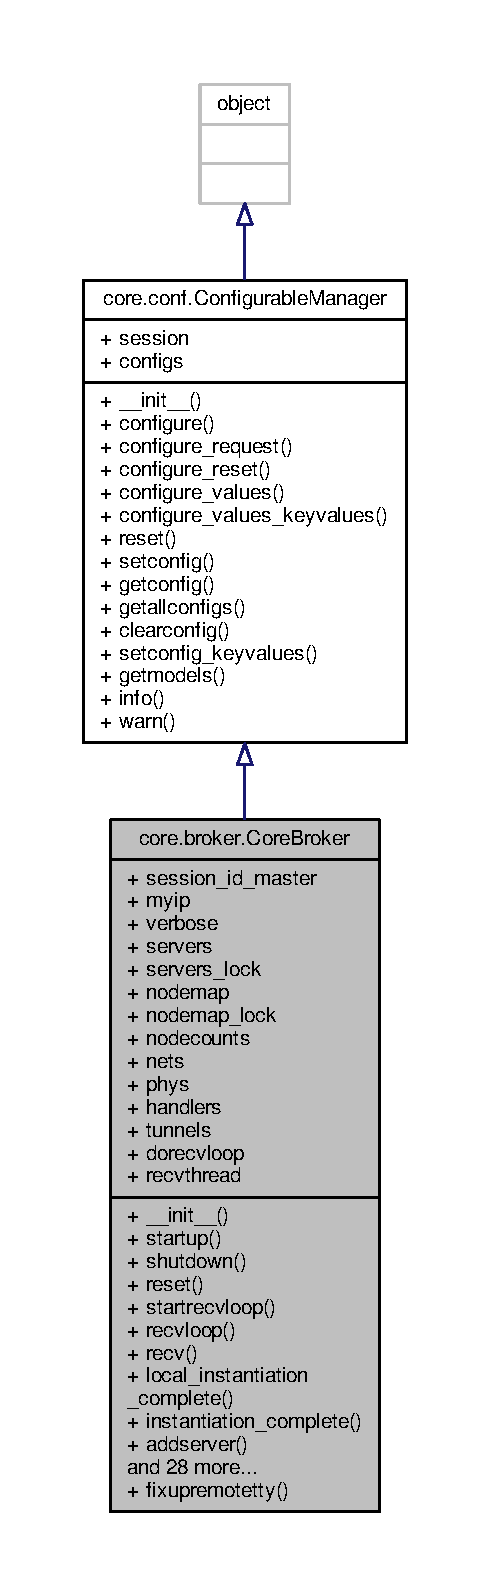
\includegraphics[height=550pt]{classcore_1_1broker_1_1_core_broker__inherit__graph}
\end{center}
\end{figure}


Collaboration diagram for core.\+broker.\+Core\+Broker\+:
\nopagebreak
\begin{figure}[H]
\begin{center}
\leavevmode
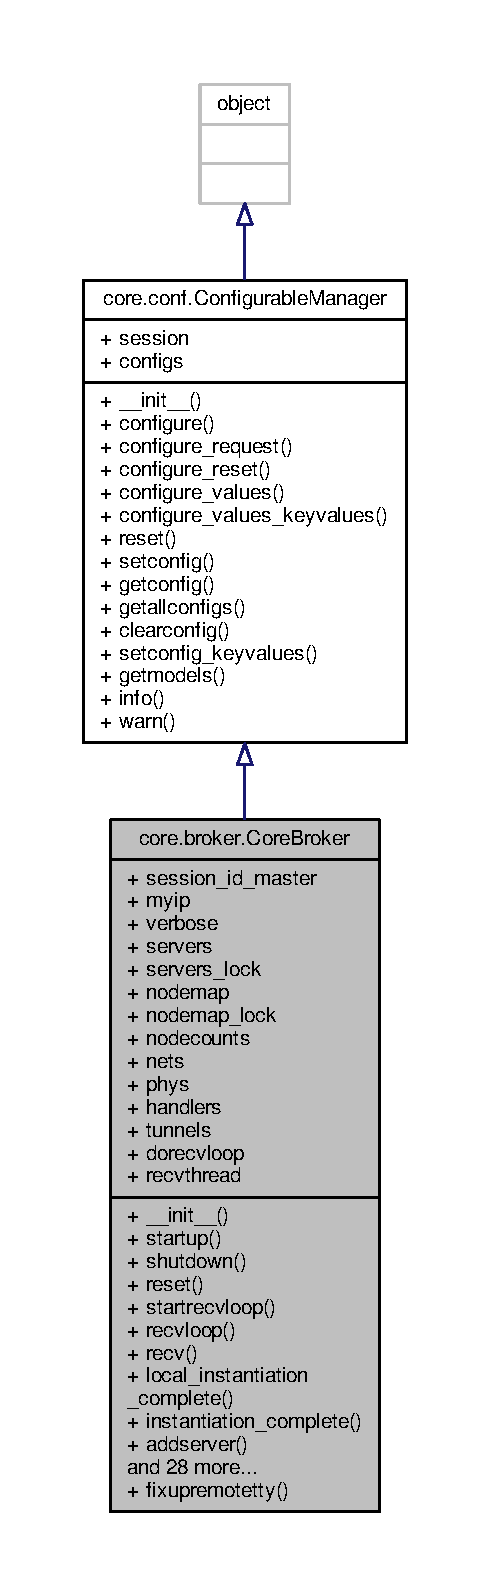
\includegraphics[height=550pt]{classcore_1_1broker_1_1_core_broker__coll__graph}
\end{center}
\end{figure}
\subsection*{Public Member Functions}
\begin{DoxyCompactItemize}
\item 
\hypertarget{classcore_1_1broker_1_1_core_broker_a935f310d4e45e54f59d0dfcb7805e632}{def {\bfseries \+\_\+\+\_\+init\+\_\+\+\_\+}}\label{classcore_1_1broker_1_1_core_broker_a935f310d4e45e54f59d0dfcb7805e632}

\item 
def \hyperlink{classcore_1_1broker_1_1_core_broker_ae374c068e0d1e2a0fdd02e97542efd16}{startup}
\item 
def \hyperlink{classcore_1_1broker_1_1_core_broker_a183821253455e288e4ed9be8ba4d5904}{shutdown}
\item 
def \hyperlink{classcore_1_1broker_1_1_core_broker_ae1fc05cfb6afecd8550cfe06bd6e034b}{reset}
\item 
def \hyperlink{classcore_1_1broker_1_1_core_broker_a89db0e240cc1f9870dfa54f6a8596abc}{startrecvloop}
\item 
def \hyperlink{classcore_1_1broker_1_1_core_broker_a3c11034b5f2a9c94117d7dfcd7b363af}{recvloop}
\item 
def \hyperlink{classcore_1_1broker_1_1_core_broker_ad900031736d366fcccb841aeb682f45b}{recv}
\item 
def \hyperlink{classcore_1_1broker_1_1_core_broker_a9bc2b4e24f6a971637fa7015129ccd6e}{local\+\_\+instantiation\+\_\+complete}
\item 
def \hyperlink{classcore_1_1broker_1_1_core_broker_a4beb718cd6597f4ecfed95bfc6691ea1}{instantiation\+\_\+complete}
\item 
def \hyperlink{classcore_1_1broker_1_1_core_broker_ab49a42fe492f71945c77b51d90b9796c}{addserver}
\item 
def \hyperlink{classcore_1_1broker_1_1_core_broker_afb27f84a0be44ebf4d8a6c3d0ed50f62}{delserver}
\item 
def \hyperlink{classcore_1_1broker_1_1_core_broker_aa4511f4a854b5c75e70468312f42070b}{getserverbyname}
\item 
def \hyperlink{classcore_1_1broker_1_1_core_broker_a8a3cc9cca90ece2ddeea874040837c0e}{getserverbysock}
\item 
def \hyperlink{classcore_1_1broker_1_1_core_broker_aa181fc886fa0b49f33e3183513d0a7a6}{getservers}
\item 
def \hyperlink{classcore_1_1broker_1_1_core_broker_a4546c152527cb9a528339a99d73a7ea6}{getservernames}
\item 
def \hyperlink{classcore_1_1broker_1_1_core_broker_ae87c24f64a0cb6422679ce135edd4c97}{tunnelkey}
\item 
def \hyperlink{classcore_1_1broker_1_1_core_broker_a1b855f94bef2565eb8282de25ff11122}{addtunnel}
\item 
def \hyperlink{classcore_1_1broker_1_1_core_broker_ac291295f26264962f4bdddcb9673c0d1}{addnettunnels}
\item 
\hypertarget{classcore_1_1broker_1_1_core_broker_ae8d0bd37b367284037fa39e0afb85f27}{def {\bfseries addnettunnel}}\label{classcore_1_1broker_1_1_core_broker_ae8d0bd37b367284037fa39e0afb85f27}

\item 
def \hyperlink{classcore_1_1broker_1_1_core_broker_a89b852636a86422e8af5e9b3005cc896}{deltunnel}
\item 
def \hyperlink{classcore_1_1broker_1_1_core_broker_a71a8cb73d8e11c40b990d1b0b88daaf9}{gettunnel}
\item 
def \hyperlink{classcore_1_1broker_1_1_core_broker_ad57eabcf9eea1e0b3bdbe35bac9901aa}{addnodemap}
\item 
def \hyperlink{classcore_1_1broker_1_1_core_broker_aeee6b763481c8c6e5190f8819186eb34}{delnodemap}
\item 
def \hyperlink{classcore_1_1broker_1_1_core_broker_aec3a34734f2617ec1fceedae93f42776}{getserversbynode}
\item 
def \hyperlink{classcore_1_1broker_1_1_core_broker_ac315dd60a4baecbb130eb05542d18e08}{addnet}
\item 
def \hyperlink{classcore_1_1broker_1_1_core_broker_a94c61d1f04e55949980131c04f53135d}{addphys}
\item 
def \hyperlink{classcore_1_1broker_1_1_core_broker_a1fe86cfe817308b36f39c1be0bdb0866}{configure\+\_\+reset}
\item 
def \hyperlink{classcore_1_1broker_1_1_core_broker_a41bb45e96f171d1bc4572fc2e488693b}{configure\+\_\+values}
\item 
def \hyperlink{classcore_1_1broker_1_1_core_broker_a6801ecce1e0f61a53aad3305ef15a4f3}{handlemsg}
\item 
def \hyperlink{classcore_1_1broker_1_1_core_broker_acbadbdbf79ce9408c7bd38e2a805642d}{setupserver}
\item 
def \hyperlink{classcore_1_1broker_1_1_core_broker_a8f67805cce8f00d0b094ce18a0234224}{handlenodemsg}
\item 
def \hyperlink{classcore_1_1broker_1_1_core_broker_a8fb4f2214cbbca69b816afaaf52d8a1c}{handlelinkmsg}
\item 
def \hyperlink{classcore_1_1broker_1_1_core_broker_a25f849874d957dbd23ad42ff21dd35f1}{addlinkendpoints}
\item 
def \hyperlink{classcore_1_1broker_1_1_core_broker_a484a8e4f7c4bb007e19cf8961a9f344f}{getlinkendpoint}
\item 
def \hyperlink{classcore_1_1broker_1_1_core_broker_a63d6e4cd3270ceb6ffc63cd2cb3ad978}{handlerawmsg}
\item 
def \hyperlink{classcore_1_1broker_1_1_core_broker_a4672e8216887d50b3b01948e785fa1b3}{forwardmsg}
\item 
def \hyperlink{classcore_1_1broker_1_1_core_broker_ae832820695b78e7231df26455c037c60}{writeservers}
\item 
def \hyperlink{classcore_1_1broker_1_1_core_broker_a8dbecc71f839abe5c002de6e00d27945}{writenodeserver}
\end{DoxyCompactItemize}
\subsection*{Static Public Member Functions}
\begin{DoxyCompactItemize}
\item 
def \hyperlink{classcore_1_1broker_1_1_core_broker_ae20748006a43afe488d3451bdad9759b}{fixupremotetty}
\end{DoxyCompactItemize}
\subsection*{Public Attributes}
\begin{DoxyCompactItemize}
\item 
\hypertarget{classcore_1_1broker_1_1_core_broker_a01e3c7ba570e019db18b109931e3fd22}{{\bfseries session\+\_\+id\+\_\+master}}\label{classcore_1_1broker_1_1_core_broker_a01e3c7ba570e019db18b109931e3fd22}

\item 
\hypertarget{classcore_1_1broker_1_1_core_broker_a4b7abc2619a2f1f6d43f0802e80760c0}{{\bfseries myip}}\label{classcore_1_1broker_1_1_core_broker_a4b7abc2619a2f1f6d43f0802e80760c0}

\item 
\hypertarget{classcore_1_1broker_1_1_core_broker_a93794410b832e001ddf7493655032818}{{\bfseries verbose}}\label{classcore_1_1broker_1_1_core_broker_a93794410b832e001ddf7493655032818}

\item 
\hypertarget{classcore_1_1broker_1_1_core_broker_a8b96c9a427ea1a46a3ddbf58a590a73b}{{\bfseries servers}}\label{classcore_1_1broker_1_1_core_broker_a8b96c9a427ea1a46a3ddbf58a590a73b}

\item 
\hypertarget{classcore_1_1broker_1_1_core_broker_a465cbcfa48286ec6a19b1ec54d42941f}{{\bfseries servers\+\_\+lock}}\label{classcore_1_1broker_1_1_core_broker_a465cbcfa48286ec6a19b1ec54d42941f}

\item 
\hypertarget{classcore_1_1broker_1_1_core_broker_a727b7274501da7807c995c3a9c93549d}{{\bfseries nodemap}}\label{classcore_1_1broker_1_1_core_broker_a727b7274501da7807c995c3a9c93549d}

\item 
\hypertarget{classcore_1_1broker_1_1_core_broker_a52566fd1fbcb3efa79cc29774bcc7781}{{\bfseries nodemap\+\_\+lock}}\label{classcore_1_1broker_1_1_core_broker_a52566fd1fbcb3efa79cc29774bcc7781}

\item 
\hypertarget{classcore_1_1broker_1_1_core_broker_a54006ad1eb2aac7a9671e4f7cc6bc7fc}{{\bfseries nodecounts}}\label{classcore_1_1broker_1_1_core_broker_a54006ad1eb2aac7a9671e4f7cc6bc7fc}

\item 
\hypertarget{classcore_1_1broker_1_1_core_broker_aa48b944c323520f1dd9ed4e2558a34c4}{{\bfseries nets}}\label{classcore_1_1broker_1_1_core_broker_aa48b944c323520f1dd9ed4e2558a34c4}

\item 
\hypertarget{classcore_1_1broker_1_1_core_broker_a927ce4debaf14fadf55ab10daed9645d}{{\bfseries phys}}\label{classcore_1_1broker_1_1_core_broker_a927ce4debaf14fadf55ab10daed9645d}

\item 
\hypertarget{classcore_1_1broker_1_1_core_broker_add811170458c1c3b9cf3d6b0ba0fec34}{{\bfseries handlers}}\label{classcore_1_1broker_1_1_core_broker_add811170458c1c3b9cf3d6b0ba0fec34}

\item 
\hypertarget{classcore_1_1broker_1_1_core_broker_acd5f314fd5c4e79dd613207235922b3b}{{\bfseries tunnels}}\label{classcore_1_1broker_1_1_core_broker_acd5f314fd5c4e79dd613207235922b3b}

\item 
\hypertarget{classcore_1_1broker_1_1_core_broker_ae8023f84783cb5f3630249127fae5613}{{\bfseries dorecvloop}}\label{classcore_1_1broker_1_1_core_broker_ae8023f84783cb5f3630249127fae5613}

\item 
\hypertarget{classcore_1_1broker_1_1_core_broker_a6534a4c280fa3222c19281109b05f0c6}{{\bfseries recvthread}}\label{classcore_1_1broker_1_1_core_broker_a6534a4c280fa3222c19281109b05f0c6}

\end{DoxyCompactItemize}


\subsection{Detailed Description}
\begin{DoxyVerb}Member of pycore session class for handling global emulation server
    data.
\end{DoxyVerb}
 

\subsection{Member Function Documentation}
\hypertarget{classcore_1_1broker_1_1_core_broker_a25f849874d957dbd23ad42ff21dd35f1}{\index{core\+::broker\+::\+Core\+Broker@{core\+::broker\+::\+Core\+Broker}!addlinkendpoints@{addlinkendpoints}}
\index{addlinkendpoints@{addlinkendpoints}!core\+::broker\+::\+Core\+Broker@{core\+::broker\+::\+Core\+Broker}}
\subsubsection[{addlinkendpoints}]{\setlength{\rightskip}{0pt plus 5cm}def core.\+broker.\+Core\+Broker.\+addlinkendpoints (
\begin{DoxyParamCaption}
\item[{}]{self, }
\item[{}]{msg, }
\item[{}]{servers1, }
\item[{}]{servers2}
\end{DoxyParamCaption}
)}}\label{classcore_1_1broker_1_1_core_broker_a25f849874d957dbd23ad42ff21dd35f1}
\begin{DoxyVerb}For a link message that is not handled locally, inform the remote
    servers of the IP addresses used as tunnel endpoints by adding
    opaque data to the link message.
\end{DoxyVerb}
 \hypertarget{classcore_1_1broker_1_1_core_broker_ac315dd60a4baecbb130eb05542d18e08}{\index{core\+::broker\+::\+Core\+Broker@{core\+::broker\+::\+Core\+Broker}!addnet@{addnet}}
\index{addnet@{addnet}!core\+::broker\+::\+Core\+Broker@{core\+::broker\+::\+Core\+Broker}}
\subsubsection[{addnet}]{\setlength{\rightskip}{0pt plus 5cm}def core.\+broker.\+Core\+Broker.\+addnet (
\begin{DoxyParamCaption}
\item[{}]{self, }
\item[{}]{nodenum}
\end{DoxyParamCaption}
)}}\label{classcore_1_1broker_1_1_core_broker_ac315dd60a4baecbb130eb05542d18e08}
\begin{DoxyVerb}Add a node number to the list of link-layer nodes.
\end{DoxyVerb}
 \hypertarget{classcore_1_1broker_1_1_core_broker_ac291295f26264962f4bdddcb9673c0d1}{\index{core\+::broker\+::\+Core\+Broker@{core\+::broker\+::\+Core\+Broker}!addnettunnels@{addnettunnels}}
\index{addnettunnels@{addnettunnels}!core\+::broker\+::\+Core\+Broker@{core\+::broker\+::\+Core\+Broker}}
\subsubsection[{addnettunnels}]{\setlength{\rightskip}{0pt plus 5cm}def core.\+broker.\+Core\+Broker.\+addnettunnels (
\begin{DoxyParamCaption}
\item[{}]{self}
\end{DoxyParamCaption}
)}}\label{classcore_1_1broker_1_1_core_broker_ac291295f26264962f4bdddcb9673c0d1}
\begin{DoxyVerb}Add GreTaps between network devices on different machines.
The GreTapBridge is not used since that would add an extra bridge.
\end{DoxyVerb}
 \hypertarget{classcore_1_1broker_1_1_core_broker_ad57eabcf9eea1e0b3bdbe35bac9901aa}{\index{core\+::broker\+::\+Core\+Broker@{core\+::broker\+::\+Core\+Broker}!addnodemap@{addnodemap}}
\index{addnodemap@{addnodemap}!core\+::broker\+::\+Core\+Broker@{core\+::broker\+::\+Core\+Broker}}
\subsubsection[{addnodemap}]{\setlength{\rightskip}{0pt plus 5cm}def core.\+broker.\+Core\+Broker.\+addnodemap (
\begin{DoxyParamCaption}
\item[{}]{self, }
\item[{}]{server, }
\item[{}]{nodenum}
\end{DoxyParamCaption}
)}}\label{classcore_1_1broker_1_1_core_broker_ad57eabcf9eea1e0b3bdbe35bac9901aa}
\begin{DoxyVerb}Record a node number to emulation server mapping.
\end{DoxyVerb}
 \hypertarget{classcore_1_1broker_1_1_core_broker_a94c61d1f04e55949980131c04f53135d}{\index{core\+::broker\+::\+Core\+Broker@{core\+::broker\+::\+Core\+Broker}!addphys@{addphys}}
\index{addphys@{addphys}!core\+::broker\+::\+Core\+Broker@{core\+::broker\+::\+Core\+Broker}}
\subsubsection[{addphys}]{\setlength{\rightskip}{0pt plus 5cm}def core.\+broker.\+Core\+Broker.\+addphys (
\begin{DoxyParamCaption}
\item[{}]{self, }
\item[{}]{nodenum}
\end{DoxyParamCaption}
)}}\label{classcore_1_1broker_1_1_core_broker_a94c61d1f04e55949980131c04f53135d}
\begin{DoxyVerb}Add a node number to the list of physical nodes.
\end{DoxyVerb}
 \hypertarget{classcore_1_1broker_1_1_core_broker_ab49a42fe492f71945c77b51d90b9796c}{\index{core\+::broker\+::\+Core\+Broker@{core\+::broker\+::\+Core\+Broker}!addserver@{addserver}}
\index{addserver@{addserver}!core\+::broker\+::\+Core\+Broker@{core\+::broker\+::\+Core\+Broker}}
\subsubsection[{addserver}]{\setlength{\rightskip}{0pt plus 5cm}def core.\+broker.\+Core\+Broker.\+addserver (
\begin{DoxyParamCaption}
\item[{}]{self, }
\item[{}]{name, }
\item[{}]{host, }
\item[{}]{port}
\end{DoxyParamCaption}
)}}\label{classcore_1_1broker_1_1_core_broker_ab49a42fe492f71945c77b51d90b9796c}
\begin{DoxyVerb}Add a new server, and try to connect to it. If we're already
    connected to this (host, port), then leave it alone. When host,port
    is None, do not try to connect.
\end{DoxyVerb}
 \hypertarget{classcore_1_1broker_1_1_core_broker_a1b855f94bef2565eb8282de25ff11122}{\index{core\+::broker\+::\+Core\+Broker@{core\+::broker\+::\+Core\+Broker}!addtunnel@{addtunnel}}
\index{addtunnel@{addtunnel}!core\+::broker\+::\+Core\+Broker@{core\+::broker\+::\+Core\+Broker}}
\subsubsection[{addtunnel}]{\setlength{\rightskip}{0pt plus 5cm}def core.\+broker.\+Core\+Broker.\+addtunnel (
\begin{DoxyParamCaption}
\item[{}]{self, }
\item[{}]{remoteip, }
\item[{}]{n1num, }
\item[{}]{n2num, }
\item[{}]{localnum}
\end{DoxyParamCaption}
)}}\label{classcore_1_1broker_1_1_core_broker_a1b855f94bef2565eb8282de25ff11122}
\begin{DoxyVerb}Add a new GreTapBridge between nodes on two different machines.
\end{DoxyVerb}
 \hypertarget{classcore_1_1broker_1_1_core_broker_a1fe86cfe817308b36f39c1be0bdb0866}{\index{core\+::broker\+::\+Core\+Broker@{core\+::broker\+::\+Core\+Broker}!configure\+\_\+reset@{configure\+\_\+reset}}
\index{configure\+\_\+reset@{configure\+\_\+reset}!core\+::broker\+::\+Core\+Broker@{core\+::broker\+::\+Core\+Broker}}
\subsubsection[{configure\+\_\+reset}]{\setlength{\rightskip}{0pt plus 5cm}def core.\+broker.\+Core\+Broker.\+configure\+\_\+reset (
\begin{DoxyParamCaption}
\item[{}]{self, }
\item[{}]{msg}
\end{DoxyParamCaption}
)}}\label{classcore_1_1broker_1_1_core_broker_a1fe86cfe817308b36f39c1be0bdb0866}
\begin{DoxyVerb}Ignore reset messages, because node delete responses may still 
    arrive and require the use of nodecounts.
\end{DoxyVerb}
 \hypertarget{classcore_1_1broker_1_1_core_broker_a41bb45e96f171d1bc4572fc2e488693b}{\index{core\+::broker\+::\+Core\+Broker@{core\+::broker\+::\+Core\+Broker}!configure\+\_\+values@{configure\+\_\+values}}
\index{configure\+\_\+values@{configure\+\_\+values}!core\+::broker\+::\+Core\+Broker@{core\+::broker\+::\+Core\+Broker}}
\subsubsection[{configure\+\_\+values}]{\setlength{\rightskip}{0pt plus 5cm}def core.\+broker.\+Core\+Broker.\+configure\+\_\+values (
\begin{DoxyParamCaption}
\item[{}]{self, }
\item[{}]{msg, }
\item[{}]{values}
\end{DoxyParamCaption}
)}}\label{classcore_1_1broker_1_1_core_broker_a41bb45e96f171d1bc4572fc2e488693b}
\begin{DoxyVerb}Receive configuration message with a list of server:host:port
    combinations that we'll need to connect with.
\end{DoxyVerb}
 \hypertarget{classcore_1_1broker_1_1_core_broker_aeee6b763481c8c6e5190f8819186eb34}{\index{core\+::broker\+::\+Core\+Broker@{core\+::broker\+::\+Core\+Broker}!delnodemap@{delnodemap}}
\index{delnodemap@{delnodemap}!core\+::broker\+::\+Core\+Broker@{core\+::broker\+::\+Core\+Broker}}
\subsubsection[{delnodemap}]{\setlength{\rightskip}{0pt plus 5cm}def core.\+broker.\+Core\+Broker.\+delnodemap (
\begin{DoxyParamCaption}
\item[{}]{self, }
\item[{}]{server, }
\item[{}]{nodenum}
\end{DoxyParamCaption}
)}}\label{classcore_1_1broker_1_1_core_broker_aeee6b763481c8c6e5190f8819186eb34}
\begin{DoxyVerb}Remove a node number to emulation server mapping.
    Return the number of nodes left on this server.
\end{DoxyVerb}
 \hypertarget{classcore_1_1broker_1_1_core_broker_afb27f84a0be44ebf4d8a6c3d0ed50f62}{\index{core\+::broker\+::\+Core\+Broker@{core\+::broker\+::\+Core\+Broker}!delserver@{delserver}}
\index{delserver@{delserver}!core\+::broker\+::\+Core\+Broker@{core\+::broker\+::\+Core\+Broker}}
\subsubsection[{delserver}]{\setlength{\rightskip}{0pt plus 5cm}def core.\+broker.\+Core\+Broker.\+delserver (
\begin{DoxyParamCaption}
\item[{}]{self, }
\item[{}]{server}
\end{DoxyParamCaption}
)}}\label{classcore_1_1broker_1_1_core_broker_afb27f84a0be44ebf4d8a6c3d0ed50f62}
\begin{DoxyVerb}Remove a server and hang up any connection.
\end{DoxyVerb}
 \hypertarget{classcore_1_1broker_1_1_core_broker_a89b852636a86422e8af5e9b3005cc896}{\index{core\+::broker\+::\+Core\+Broker@{core\+::broker\+::\+Core\+Broker}!deltunnel@{deltunnel}}
\index{deltunnel@{deltunnel}!core\+::broker\+::\+Core\+Broker@{core\+::broker\+::\+Core\+Broker}}
\subsubsection[{deltunnel}]{\setlength{\rightskip}{0pt plus 5cm}def core.\+broker.\+Core\+Broker.\+deltunnel (
\begin{DoxyParamCaption}
\item[{}]{self, }
\item[{}]{n1num, }
\item[{}]{n2num}
\end{DoxyParamCaption}
)}}\label{classcore_1_1broker_1_1_core_broker_a89b852636a86422e8af5e9b3005cc896}
\begin{DoxyVerb}Cleanup of the GreTapBridge.
\end{DoxyVerb}
 \hypertarget{classcore_1_1broker_1_1_core_broker_ae20748006a43afe488d3451bdad9759b}{\index{core\+::broker\+::\+Core\+Broker@{core\+::broker\+::\+Core\+Broker}!fixupremotetty@{fixupremotetty}}
\index{fixupremotetty@{fixupremotetty}!core\+::broker\+::\+Core\+Broker@{core\+::broker\+::\+Core\+Broker}}
\subsubsection[{fixupremotetty}]{\setlength{\rightskip}{0pt plus 5cm}def core.\+broker.\+Core\+Broker.\+fixupremotetty (
\begin{DoxyParamCaption}
\item[{}]{msghdr, }
\item[{}]{msgdata, }
\item[{}]{host}
\end{DoxyParamCaption}
)\hspace{0.3cm}{\ttfamily [static]}}}\label{classcore_1_1broker_1_1_core_broker_ae20748006a43afe488d3451bdad9759b}
\begin{DoxyVerb}When an interactive TTY request comes from the GUI, snoop the reply
    and add an SSH command to the appropriate remote server.
\end{DoxyVerb}
 \hypertarget{classcore_1_1broker_1_1_core_broker_a4672e8216887d50b3b01948e785fa1b3}{\index{core\+::broker\+::\+Core\+Broker@{core\+::broker\+::\+Core\+Broker}!forwardmsg@{forwardmsg}}
\index{forwardmsg@{forwardmsg}!core\+::broker\+::\+Core\+Broker@{core\+::broker\+::\+Core\+Broker}}
\subsubsection[{forwardmsg}]{\setlength{\rightskip}{0pt plus 5cm}def core.\+broker.\+Core\+Broker.\+forwardmsg (
\begin{DoxyParamCaption}
\item[{}]{self, }
\item[{}]{msg, }
\item[{}]{servers}
\end{DoxyParamCaption}
)}}\label{classcore_1_1broker_1_1_core_broker_a4672e8216887d50b3b01948e785fa1b3}
\begin{DoxyVerb}Forward API message to all given servers.

    Return True if an empty host/port is encountered, indicating
    the message should be handled locally.
\end{DoxyVerb}
 \hypertarget{classcore_1_1broker_1_1_core_broker_a484a8e4f7c4bb007e19cf8961a9f344f}{\index{core\+::broker\+::\+Core\+Broker@{core\+::broker\+::\+Core\+Broker}!getlinkendpoint@{getlinkendpoint}}
\index{getlinkendpoint@{getlinkendpoint}!core\+::broker\+::\+Core\+Broker@{core\+::broker\+::\+Core\+Broker}}
\subsubsection[{getlinkendpoint}]{\setlength{\rightskip}{0pt plus 5cm}def core.\+broker.\+Core\+Broker.\+getlinkendpoint (
\begin{DoxyParamCaption}
\item[{}]{self, }
\item[{}]{msg, }
\item[{}]{first\+\_\+is\+\_\+local}
\end{DoxyParamCaption}
)}}\label{classcore_1_1broker_1_1_core_broker_a484a8e4f7c4bb007e19cf8961a9f344f}
\begin{DoxyVerb}A link message between two different servers has been received,
    and we need to determine the tunnel endpoint. First look for
    opaque data in the link message, otherwise use the IP of the message
    sender (the master server).
\end{DoxyVerb}
 \hypertarget{classcore_1_1broker_1_1_core_broker_aa4511f4a854b5c75e70468312f42070b}{\index{core\+::broker\+::\+Core\+Broker@{core\+::broker\+::\+Core\+Broker}!getserverbyname@{getserverbyname}}
\index{getserverbyname@{getserverbyname}!core\+::broker\+::\+Core\+Broker@{core\+::broker\+::\+Core\+Broker}}
\subsubsection[{getserverbyname}]{\setlength{\rightskip}{0pt plus 5cm}def core.\+broker.\+Core\+Broker.\+getserverbyname (
\begin{DoxyParamCaption}
\item[{}]{self, }
\item[{}]{name}
\end{DoxyParamCaption}
)}}\label{classcore_1_1broker_1_1_core_broker_aa4511f4a854b5c75e70468312f42070b}
\begin{DoxyVerb}Return the server object having the given name, or None.
\end{DoxyVerb}
 \hypertarget{classcore_1_1broker_1_1_core_broker_a8a3cc9cca90ece2ddeea874040837c0e}{\index{core\+::broker\+::\+Core\+Broker@{core\+::broker\+::\+Core\+Broker}!getserverbysock@{getserverbysock}}
\index{getserverbysock@{getserverbysock}!core\+::broker\+::\+Core\+Broker@{core\+::broker\+::\+Core\+Broker}}
\subsubsection[{getserverbysock}]{\setlength{\rightskip}{0pt plus 5cm}def core.\+broker.\+Core\+Broker.\+getserverbysock (
\begin{DoxyParamCaption}
\item[{}]{self, }
\item[{}]{sock}
\end{DoxyParamCaption}
)}}\label{classcore_1_1broker_1_1_core_broker_a8a3cc9cca90ece2ddeea874040837c0e}
\begin{DoxyVerb}Return the server object corresponding to the given socket,
    or None.
\end{DoxyVerb}
 \hypertarget{classcore_1_1broker_1_1_core_broker_a4546c152527cb9a528339a99d73a7ea6}{\index{core\+::broker\+::\+Core\+Broker@{core\+::broker\+::\+Core\+Broker}!getservernames@{getservernames}}
\index{getservernames@{getservernames}!core\+::broker\+::\+Core\+Broker@{core\+::broker\+::\+Core\+Broker}}
\subsubsection[{getservernames}]{\setlength{\rightskip}{0pt plus 5cm}def core.\+broker.\+Core\+Broker.\+getservernames (
\begin{DoxyParamCaption}
\item[{}]{self}
\end{DoxyParamCaption}
)}}\label{classcore_1_1broker_1_1_core_broker_a4546c152527cb9a528339a99d73a7ea6}
\begin{DoxyVerb}Return a sorted list of server names (keys from self.servers).
\end{DoxyVerb}
 \hypertarget{classcore_1_1broker_1_1_core_broker_aa181fc886fa0b49f33e3183513d0a7a6}{\index{core\+::broker\+::\+Core\+Broker@{core\+::broker\+::\+Core\+Broker}!getservers@{getservers}}
\index{getservers@{getservers}!core\+::broker\+::\+Core\+Broker@{core\+::broker\+::\+Core\+Broker}}
\subsubsection[{getservers}]{\setlength{\rightskip}{0pt plus 5cm}def core.\+broker.\+Core\+Broker.\+getservers (
\begin{DoxyParamCaption}
\item[{}]{self}
\end{DoxyParamCaption}
)}}\label{classcore_1_1broker_1_1_core_broker_aa181fc886fa0b49f33e3183513d0a7a6}
\begin{DoxyVerb}Return a list of servers sorted by name.\end{DoxyVerb}
 \hypertarget{classcore_1_1broker_1_1_core_broker_aec3a34734f2617ec1fceedae93f42776}{\index{core\+::broker\+::\+Core\+Broker@{core\+::broker\+::\+Core\+Broker}!getserversbynode@{getserversbynode}}
\index{getserversbynode@{getserversbynode}!core\+::broker\+::\+Core\+Broker@{core\+::broker\+::\+Core\+Broker}}
\subsubsection[{getserversbynode}]{\setlength{\rightskip}{0pt plus 5cm}def core.\+broker.\+Core\+Broker.\+getserversbynode (
\begin{DoxyParamCaption}
\item[{}]{self, }
\item[{}]{nodenum}
\end{DoxyParamCaption}
)}}\label{classcore_1_1broker_1_1_core_broker_aec3a34734f2617ec1fceedae93f42776}
\begin{DoxyVerb}Retrieve a set of emulation servers given a node number.
\end{DoxyVerb}
 \hypertarget{classcore_1_1broker_1_1_core_broker_a71a8cb73d8e11c40b990d1b0b88daaf9}{\index{core\+::broker\+::\+Core\+Broker@{core\+::broker\+::\+Core\+Broker}!gettunnel@{gettunnel}}
\index{gettunnel@{gettunnel}!core\+::broker\+::\+Core\+Broker@{core\+::broker\+::\+Core\+Broker}}
\subsubsection[{gettunnel}]{\setlength{\rightskip}{0pt plus 5cm}def core.\+broker.\+Core\+Broker.\+gettunnel (
\begin{DoxyParamCaption}
\item[{}]{self, }
\item[{}]{n1num, }
\item[{}]{n2num}
\end{DoxyParamCaption}
)}}\label{classcore_1_1broker_1_1_core_broker_a71a8cb73d8e11c40b990d1b0b88daaf9}
\begin{DoxyVerb}Return the GreTap between two nodes if it exists.
\end{DoxyVerb}
 \hypertarget{classcore_1_1broker_1_1_core_broker_a8fb4f2214cbbca69b816afaaf52d8a1c}{\index{core\+::broker\+::\+Core\+Broker@{core\+::broker\+::\+Core\+Broker}!handlelinkmsg@{handlelinkmsg}}
\index{handlelinkmsg@{handlelinkmsg}!core\+::broker\+::\+Core\+Broker@{core\+::broker\+::\+Core\+Broker}}
\subsubsection[{handlelinkmsg}]{\setlength{\rightskip}{0pt plus 5cm}def core.\+broker.\+Core\+Broker.\+handlelinkmsg (
\begin{DoxyParamCaption}
\item[{}]{self, }
\item[{}]{msg}
\end{DoxyParamCaption}
)}}\label{classcore_1_1broker_1_1_core_broker_a8fb4f2214cbbca69b816afaaf52d8a1c}
\begin{DoxyVerb}Determine and return the servers to which this link message should
    be forwarded. Also build tunnels between different servers or add
    opaque data to the link message before forwarding.
\end{DoxyVerb}
 \hypertarget{classcore_1_1broker_1_1_core_broker_a6801ecce1e0f61a53aad3305ef15a4f3}{\index{core\+::broker\+::\+Core\+Broker@{core\+::broker\+::\+Core\+Broker}!handlemsg@{handlemsg}}
\index{handlemsg@{handlemsg}!core\+::broker\+::\+Core\+Broker@{core\+::broker\+::\+Core\+Broker}}
\subsubsection[{handlemsg}]{\setlength{\rightskip}{0pt plus 5cm}def core.\+broker.\+Core\+Broker.\+handlemsg (
\begin{DoxyParamCaption}
\item[{}]{self, }
\item[{}]{msg}
\end{DoxyParamCaption}
)}}\label{classcore_1_1broker_1_1_core_broker_a6801ecce1e0f61a53aad3305ef15a4f3}
\begin{DoxyVerb}Handle an API message. Determine whether this needs to be handled
    by the local server or forwarded on to another one.
    Returns True when message does not need to be handled locally,
    and performs forwarding if required.
    Returning False indicates this message should be handled locally.
\end{DoxyVerb}
 \hypertarget{classcore_1_1broker_1_1_core_broker_a8f67805cce8f00d0b094ce18a0234224}{\index{core\+::broker\+::\+Core\+Broker@{core\+::broker\+::\+Core\+Broker}!handlenodemsg@{handlenodemsg}}
\index{handlenodemsg@{handlenodemsg}!core\+::broker\+::\+Core\+Broker@{core\+::broker\+::\+Core\+Broker}}
\subsubsection[{handlenodemsg}]{\setlength{\rightskip}{0pt plus 5cm}def core.\+broker.\+Core\+Broker.\+handlenodemsg (
\begin{DoxyParamCaption}
\item[{}]{self, }
\item[{}]{msg}
\end{DoxyParamCaption}
)}}\label{classcore_1_1broker_1_1_core_broker_a8f67805cce8f00d0b094ce18a0234224}
\begin{DoxyVerb}Determine and return the servers to which this node message should
    be forwarded. Also keep track of link-layer nodes and the mapping of
    nodes to servers.
\end{DoxyVerb}
 \hypertarget{classcore_1_1broker_1_1_core_broker_a63d6e4cd3270ceb6ffc63cd2cb3ad978}{\index{core\+::broker\+::\+Core\+Broker@{core\+::broker\+::\+Core\+Broker}!handlerawmsg@{handlerawmsg}}
\index{handlerawmsg@{handlerawmsg}!core\+::broker\+::\+Core\+Broker@{core\+::broker\+::\+Core\+Broker}}
\subsubsection[{handlerawmsg}]{\setlength{\rightskip}{0pt plus 5cm}def core.\+broker.\+Core\+Broker.\+handlerawmsg (
\begin{DoxyParamCaption}
\item[{}]{self, }
\item[{}]{msg}
\end{DoxyParamCaption}
)}}\label{classcore_1_1broker_1_1_core_broker_a63d6e4cd3270ceb6ffc63cd2cb3ad978}
\begin{DoxyVerb}Helper to invoke handlemsg() using raw (packed) message bytes.
\end{DoxyVerb}
 \hypertarget{classcore_1_1broker_1_1_core_broker_a4beb718cd6597f4ecfed95bfc6691ea1}{\index{core\+::broker\+::\+Core\+Broker@{core\+::broker\+::\+Core\+Broker}!instantiation\+\_\+complete@{instantiation\+\_\+complete}}
\index{instantiation\+\_\+complete@{instantiation\+\_\+complete}!core\+::broker\+::\+Core\+Broker@{core\+::broker\+::\+Core\+Broker}}
\subsubsection[{instantiation\+\_\+complete}]{\setlength{\rightskip}{0pt plus 5cm}def core.\+broker.\+Core\+Broker.\+instantiation\+\_\+complete (
\begin{DoxyParamCaption}
\item[{}]{self}
\end{DoxyParamCaption}
)}}\label{classcore_1_1broker_1_1_core_broker_a4beb718cd6597f4ecfed95bfc6691ea1}
\begin{DoxyVerb}\
Return True if all servers have completed instantiation, False
otherwise.
\end{DoxyVerb}
 \hypertarget{classcore_1_1broker_1_1_core_broker_a9bc2b4e24f6a971637fa7015129ccd6e}{\index{core\+::broker\+::\+Core\+Broker@{core\+::broker\+::\+Core\+Broker}!local\+\_\+instantiation\+\_\+complete@{local\+\_\+instantiation\+\_\+complete}}
\index{local\+\_\+instantiation\+\_\+complete@{local\+\_\+instantiation\+\_\+complete}!core\+::broker\+::\+Core\+Broker@{core\+::broker\+::\+Core\+Broker}}
\subsubsection[{local\+\_\+instantiation\+\_\+complete}]{\setlength{\rightskip}{0pt plus 5cm}def core.\+broker.\+Core\+Broker.\+local\+\_\+instantiation\+\_\+complete (
\begin{DoxyParamCaption}
\item[{}]{self}
\end{DoxyParamCaption}
)}}\label{classcore_1_1broker_1_1_core_broker_a9bc2b4e24f6a971637fa7015129ccd6e}
\begin{DoxyVerb}\
Set the local server's instantiation-complete status to True.
\end{DoxyVerb}
 \hypertarget{classcore_1_1broker_1_1_core_broker_ad900031736d366fcccb841aeb682f45b}{\index{core\+::broker\+::\+Core\+Broker@{core\+::broker\+::\+Core\+Broker}!recv@{recv}}
\index{recv@{recv}!core\+::broker\+::\+Core\+Broker@{core\+::broker\+::\+Core\+Broker}}
\subsubsection[{recv}]{\setlength{\rightskip}{0pt plus 5cm}def core.\+broker.\+Core\+Broker.\+recv (
\begin{DoxyParamCaption}
\item[{}]{self, }
\item[{}]{server}
\end{DoxyParamCaption}
)}}\label{classcore_1_1broker_1_1_core_broker_ad900031736d366fcccb841aeb682f45b}
\begin{DoxyVerb}Receive data on an emulation server socket and broadcast it to
    all connected session handlers. Returns the length of data recevied
    and forwarded. Return value of zero indicates the socket has closed
    and should be removed from the self.servers dict.
\end{DoxyVerb}
 \hypertarget{classcore_1_1broker_1_1_core_broker_a3c11034b5f2a9c94117d7dfcd7b363af}{\index{core\+::broker\+::\+Core\+Broker@{core\+::broker\+::\+Core\+Broker}!recvloop@{recvloop}}
\index{recvloop@{recvloop}!core\+::broker\+::\+Core\+Broker@{core\+::broker\+::\+Core\+Broker}}
\subsubsection[{recvloop}]{\setlength{\rightskip}{0pt plus 5cm}def core.\+broker.\+Core\+Broker.\+recvloop (
\begin{DoxyParamCaption}
\item[{}]{self}
\end{DoxyParamCaption}
)}}\label{classcore_1_1broker_1_1_core_broker_a3c11034b5f2a9c94117d7dfcd7b363af}
\begin{DoxyVerb}Thread target that receives messages from server sockets.
\end{DoxyVerb}
 \hypertarget{classcore_1_1broker_1_1_core_broker_ae1fc05cfb6afecd8550cfe06bd6e034b}{\index{core\+::broker\+::\+Core\+Broker@{core\+::broker\+::\+Core\+Broker}!reset@{reset}}
\index{reset@{reset}!core\+::broker\+::\+Core\+Broker@{core\+::broker\+::\+Core\+Broker}}
\subsubsection[{reset}]{\setlength{\rightskip}{0pt plus 5cm}def core.\+broker.\+Core\+Broker.\+reset (
\begin{DoxyParamCaption}
\item[{}]{self}
\end{DoxyParamCaption}
)}}\label{classcore_1_1broker_1_1_core_broker_ae1fc05cfb6afecd8550cfe06bd6e034b}
\begin{DoxyVerb}Reset to initial state.
\end{DoxyVerb}
 \hypertarget{classcore_1_1broker_1_1_core_broker_acbadbdbf79ce9408c7bd38e2a805642d}{\index{core\+::broker\+::\+Core\+Broker@{core\+::broker\+::\+Core\+Broker}!setupserver@{setupserver}}
\index{setupserver@{setupserver}!core\+::broker\+::\+Core\+Broker@{core\+::broker\+::\+Core\+Broker}}
\subsubsection[{setupserver}]{\setlength{\rightskip}{0pt plus 5cm}def core.\+broker.\+Core\+Broker.\+setupserver (
\begin{DoxyParamCaption}
\item[{}]{self, }
\item[{}]{servername}
\end{DoxyParamCaption}
)}}\label{classcore_1_1broker_1_1_core_broker_acbadbdbf79ce9408c7bd38e2a805642d}
\begin{DoxyVerb}Send the appropriate API messages for configuring the specified
    emulation server.
\end{DoxyVerb}
 \hypertarget{classcore_1_1broker_1_1_core_broker_a183821253455e288e4ed9be8ba4d5904}{\index{core\+::broker\+::\+Core\+Broker@{core\+::broker\+::\+Core\+Broker}!shutdown@{shutdown}}
\index{shutdown@{shutdown}!core\+::broker\+::\+Core\+Broker@{core\+::broker\+::\+Core\+Broker}}
\subsubsection[{shutdown}]{\setlength{\rightskip}{0pt plus 5cm}def core.\+broker.\+Core\+Broker.\+shutdown (
\begin{DoxyParamCaption}
\item[{}]{self}
\end{DoxyParamCaption}
)}}\label{classcore_1_1broker_1_1_core_broker_a183821253455e288e4ed9be8ba4d5904}
\begin{DoxyVerb}Close all active sockets; called when the session enters the
    data collect state
\end{DoxyVerb}
 \hypertarget{classcore_1_1broker_1_1_core_broker_a89db0e240cc1f9870dfa54f6a8596abc}{\index{core\+::broker\+::\+Core\+Broker@{core\+::broker\+::\+Core\+Broker}!startrecvloop@{startrecvloop}}
\index{startrecvloop@{startrecvloop}!core\+::broker\+::\+Core\+Broker@{core\+::broker\+::\+Core\+Broker}}
\subsubsection[{startrecvloop}]{\setlength{\rightskip}{0pt plus 5cm}def core.\+broker.\+Core\+Broker.\+startrecvloop (
\begin{DoxyParamCaption}
\item[{}]{self}
\end{DoxyParamCaption}
)}}\label{classcore_1_1broker_1_1_core_broker_a89db0e240cc1f9870dfa54f6a8596abc}
\begin{DoxyVerb}Spawn the recvloop() thread if it hasn't been already started.
\end{DoxyVerb}
 \hypertarget{classcore_1_1broker_1_1_core_broker_ae374c068e0d1e2a0fdd02e97542efd16}{\index{core\+::broker\+::\+Core\+Broker@{core\+::broker\+::\+Core\+Broker}!startup@{startup}}
\index{startup@{startup}!core\+::broker\+::\+Core\+Broker@{core\+::broker\+::\+Core\+Broker}}
\subsubsection[{startup}]{\setlength{\rightskip}{0pt plus 5cm}def core.\+broker.\+Core\+Broker.\+startup (
\begin{DoxyParamCaption}
\item[{}]{self}
\end{DoxyParamCaption}
)}}\label{classcore_1_1broker_1_1_core_broker_ae374c068e0d1e2a0fdd02e97542efd16}
\begin{DoxyVerb}Build tunnels between network-layer nodes now that all node
    and link information has been received; called when session
    enters the instantation state.
\end{DoxyVerb}
 \hypertarget{classcore_1_1broker_1_1_core_broker_ae87c24f64a0cb6422679ce135edd4c97}{\index{core\+::broker\+::\+Core\+Broker@{core\+::broker\+::\+Core\+Broker}!tunnelkey@{tunnelkey}}
\index{tunnelkey@{tunnelkey}!core\+::broker\+::\+Core\+Broker@{core\+::broker\+::\+Core\+Broker}}
\subsubsection[{tunnelkey}]{\setlength{\rightskip}{0pt plus 5cm}def core.\+broker.\+Core\+Broker.\+tunnelkey (
\begin{DoxyParamCaption}
\item[{}]{self, }
\item[{}]{n1num, }
\item[{}]{n2num}
\end{DoxyParamCaption}
)}}\label{classcore_1_1broker_1_1_core_broker_ae87c24f64a0cb6422679ce135edd4c97}
\begin{DoxyVerb}Compute a 32-bit key used to uniquely identify a GRE tunnel.
The hash(n1num), hash(n2num) values are used, so node numbers may be
None or string values (used for e.g. "ctrlnet").
\end{DoxyVerb}
 \hypertarget{classcore_1_1broker_1_1_core_broker_a8dbecc71f839abe5c002de6e00d27945}{\index{core\+::broker\+::\+Core\+Broker@{core\+::broker\+::\+Core\+Broker}!writenodeserver@{writenodeserver}}
\index{writenodeserver@{writenodeserver}!core\+::broker\+::\+Core\+Broker@{core\+::broker\+::\+Core\+Broker}}
\subsubsection[{writenodeserver}]{\setlength{\rightskip}{0pt plus 5cm}def core.\+broker.\+Core\+Broker.\+writenodeserver (
\begin{DoxyParamCaption}
\item[{}]{self, }
\item[{}]{nodestr, }
\item[{}]{server}
\end{DoxyParamCaption}
)}}\label{classcore_1_1broker_1_1_core_broker_a8dbecc71f839abe5c002de6e00d27945}
\begin{DoxyVerb}Creates a /tmp/pycore.nnnnn/nX.conf/server file having the node
and server info. This may be used by scripts for accessing nodes on
other machines, much like local nodes may be accessed via the
VnodeClient class.
\end{DoxyVerb}
 \hypertarget{classcore_1_1broker_1_1_core_broker_ae832820695b78e7231df26455c037c60}{\index{core\+::broker\+::\+Core\+Broker@{core\+::broker\+::\+Core\+Broker}!writeservers@{writeservers}}
\index{writeservers@{writeservers}!core\+::broker\+::\+Core\+Broker@{core\+::broker\+::\+Core\+Broker}}
\subsubsection[{writeservers}]{\setlength{\rightskip}{0pt plus 5cm}def core.\+broker.\+Core\+Broker.\+writeservers (
\begin{DoxyParamCaption}
\item[{}]{self}
\end{DoxyParamCaption}
)}}\label{classcore_1_1broker_1_1_core_broker_ae832820695b78e7231df26455c037c60}
\begin{DoxyVerb}Write the server list to a text file in the session directory upon
startup: /tmp/pycore.nnnnn/servers
\end{DoxyVerb}
 

The documentation for this class was generated from the following file\+:\begin{DoxyCompactItemize}
\item 
daemon/core/broker.\+py\end{DoxyCompactItemize}

\hypertarget{classcore_1_1api_1_1coreapi_1_1_core_conf_message}{\section{core.\+api.\+coreapi.\+Core\+Conf\+Message Class Reference}
\label{classcore_1_1api_1_1coreapi_1_1_core_conf_message}\index{core.\+api.\+coreapi.\+Core\+Conf\+Message@{core.\+api.\+coreapi.\+Core\+Conf\+Message}}
}


Inheritance diagram for core.\+api.\+coreapi.\+Core\+Conf\+Message\+:
\nopagebreak
\begin{figure}[H]
\begin{center}
\leavevmode
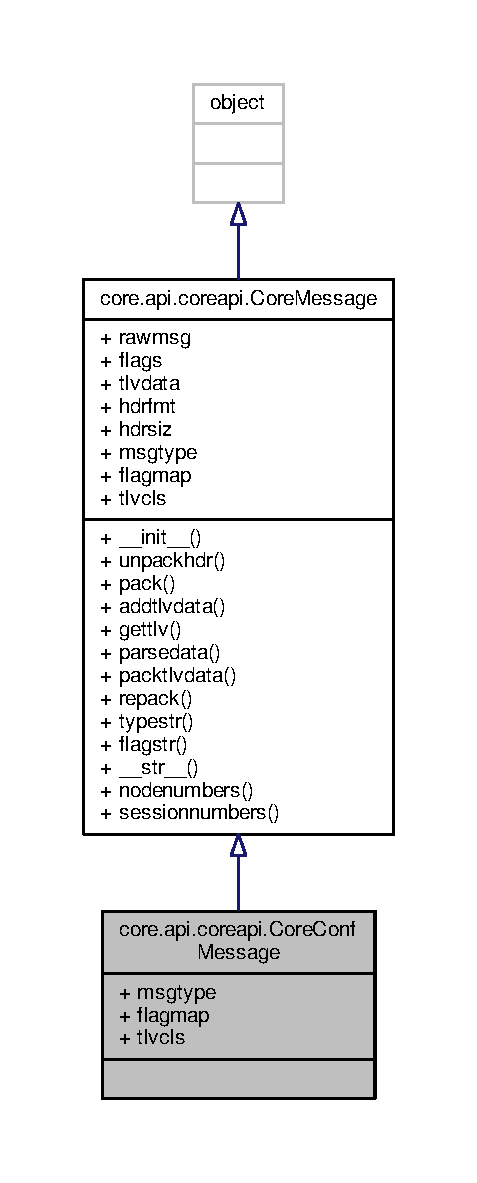
\includegraphics[height=550pt]{classcore_1_1api_1_1coreapi_1_1_core_conf_message__inherit__graph}
\end{center}
\end{figure}


Collaboration diagram for core.\+api.\+coreapi.\+Core\+Conf\+Message\+:
\nopagebreak
\begin{figure}[H]
\begin{center}
\leavevmode
\includegraphics[height=550pt]{classcore_1_1api_1_1coreapi_1_1_core_conf_message__coll__graph}
\end{center}
\end{figure}
\subsection*{Static Public Attributes}
\begin{DoxyCompactItemize}
\item 
\hypertarget{classcore_1_1api_1_1coreapi_1_1_core_conf_message_a46a8d1fac9ef18cfc1ddde7a992b70b7}{{\bfseries msgtype} = C\+O\+R\+E\+\_\+\+A\+P\+I\+\_\+\+C\+O\+N\+F\+\_\+\+M\+S\+G}\label{classcore_1_1api_1_1coreapi_1_1_core_conf_message_a46a8d1fac9ef18cfc1ddde7a992b70b7}

\item 
\hypertarget{classcore_1_1api_1_1coreapi_1_1_core_conf_message_ac8e885b9954d2d942eade13f3c671129}{{\bfseries flagmap} = message\+\_\+flags}\label{classcore_1_1api_1_1coreapi_1_1_core_conf_message_ac8e885b9954d2d942eade13f3c671129}

\item 
\hypertarget{classcore_1_1api_1_1coreapi_1_1_core_conf_message_a665523512a37546c3af2e2bd017f6dcc}{{\bfseries tlvcls} = \hyperlink{classcore_1_1api_1_1coreapi_1_1_core_conf_tlv}{Core\+Conf\+Tlv}}\label{classcore_1_1api_1_1coreapi_1_1_core_conf_message_a665523512a37546c3af2e2bd017f6dcc}

\end{DoxyCompactItemize}
\subsection*{Additional Inherited Members}


The documentation for this class was generated from the following file\+:\begin{DoxyCompactItemize}
\item 
daemon/core/api/coreapi.\+py\end{DoxyCompactItemize}

\hypertarget{classcore_1_1api_1_1coreapi_1_1_core_conf_tlv}{\section{core.\+api.\+coreapi.\+Core\+Conf\+Tlv Class Reference}
\label{classcore_1_1api_1_1coreapi_1_1_core_conf_tlv}\index{core.\+api.\+coreapi.\+Core\+Conf\+Tlv@{core.\+api.\+coreapi.\+Core\+Conf\+Tlv}}
}


Inheritance diagram for core.\+api.\+coreapi.\+Core\+Conf\+Tlv\+:
\nopagebreak
\begin{figure}[H]
\begin{center}
\leavevmode
\includegraphics[width=224pt]{classcore_1_1api_1_1coreapi_1_1_core_conf_tlv__inherit__graph}
\end{center}
\end{figure}


Collaboration diagram for core.\+api.\+coreapi.\+Core\+Conf\+Tlv\+:
\nopagebreak
\begin{figure}[H]
\begin{center}
\leavevmode
\includegraphics[width=225pt]{classcore_1_1api_1_1coreapi_1_1_core_conf_tlv__coll__graph}
\end{center}
\end{figure}
\subsection*{Static Public Attributes}
\begin{DoxyCompactItemize}
\item 
\hypertarget{classcore_1_1api_1_1coreapi_1_1_core_conf_tlv_a83a80cccd88b2cc074d6fda5147c5640}{{\bfseries tlvtypemap} = conf\+\_\+tlvs}\label{classcore_1_1api_1_1coreapi_1_1_core_conf_tlv_a83a80cccd88b2cc074d6fda5147c5640}

\item 
dictionary {\bfseries tlvdataclsmap}
\end{DoxyCompactItemize}
\subsection*{Additional Inherited Members}


\subsection{Member Data Documentation}
\hypertarget{classcore_1_1api_1_1coreapi_1_1_core_conf_tlv_a20158fbe8221bf15d311aeb8dc0988e4}{\index{core\+::api\+::coreapi\+::\+Core\+Conf\+Tlv@{core\+::api\+::coreapi\+::\+Core\+Conf\+Tlv}!tlvdataclsmap@{tlvdataclsmap}}
\index{tlvdataclsmap@{tlvdataclsmap}!core\+::api\+::coreapi\+::\+Core\+Conf\+Tlv@{core\+::api\+::coreapi\+::\+Core\+Conf\+Tlv}}
\subsubsection[{tlvdataclsmap}]{\setlength{\rightskip}{0pt plus 5cm}dictionary core.\+api.\+coreapi.\+Core\+Conf\+Tlv.\+tlvdataclsmap\hspace{0.3cm}{\ttfamily [static]}}}\label{classcore_1_1api_1_1coreapi_1_1_core_conf_tlv_a20158fbe8221bf15d311aeb8dc0988e4}
{\bfseries Initial value\+:}
\begin{DoxyCode}
1 = \{
2         CORE\_TLV\_CONF\_NODE: CoreTlvDataUint32,
3         CORE\_TLV\_CONF\_OBJ: CoreTlvDataString,
4         CORE\_TLV\_CONF\_TYPE: CoreTlvDataUint16,
5         CORE\_TLV\_CONF\_DATA\_TYPES: CoreTlvDataUint16List,
6         CORE\_TLV\_CONF\_VALUES: CoreTlvDataString,
7         CORE\_TLV\_CONF\_CAPTIONS: CoreTlvDataString,
8         CORE\_TLV\_CONF\_BITMAP: CoreTlvDataString,
9         CORE\_TLV\_CONF\_POSSIBLE\_VALUES: CoreTlvDataString,
10         CORE\_TLV\_CONF\_GROUPS: CoreTlvDataString,
11         CORE\_TLV\_CONF\_SESSION: CoreTlvDataString,
12         CORE\_TLV\_CONF\_IFNUM: CoreTlvDataUint16,
13         CORE\_TLV\_CONF\_NETID: CoreTlvDataUint32,
14         CORE\_TLV\_CONF\_OPAQUE: CoreTlvDataString, 
15     \}
\end{DoxyCode}


The documentation for this class was generated from the following file\+:\begin{DoxyCompactItemize}
\item 
daemon/core/api/coreapi.\+py\end{DoxyCompactItemize}

\hypertarget{classcore_1_1coreserver_1_1_core_datagram_request_handler}{\section{core.\+coreserver.\+Core\+Datagram\+Request\+Handler Class Reference}
\label{classcore_1_1coreserver_1_1_core_datagram_request_handler}\index{core.\+coreserver.\+Core\+Datagram\+Request\+Handler@{core.\+coreserver.\+Core\+Datagram\+Request\+Handler}}
}


Inheritance diagram for core.\+coreserver.\+Core\+Datagram\+Request\+Handler\+:
\nopagebreak
\begin{figure}[H]
\begin{center}
\leavevmode
\includegraphics[height=550pt]{classcore_1_1coreserver_1_1_core_datagram_request_handler__inherit__graph}
\end{center}
\end{figure}


Collaboration diagram for core.\+coreserver.\+Core\+Datagram\+Request\+Handler\+:
\nopagebreak
\begin{figure}[H]
\begin{center}
\leavevmode
\includegraphics[height=550pt]{classcore_1_1coreserver_1_1_core_datagram_request_handler__coll__graph}
\end{center}
\end{figure}
\subsection*{Public Member Functions}
\begin{DoxyCompactItemize}
\item 
\hypertarget{classcore_1_1coreserver_1_1_core_datagram_request_handler_ada903989e37455a48f8803c8ea6fa3d1}{def {\bfseries \+\_\+\+\_\+init\+\_\+\+\_\+}}\label{classcore_1_1coreserver_1_1_core_datagram_request_handler_ada903989e37455a48f8803c8ea6fa3d1}

\item 
def \hyperlink{classcore_1_1coreserver_1_1_core_datagram_request_handler_a55320dcbc4d6dee8ff55774587159b17}{setup}
\item 
\hypertarget{classcore_1_1coreserver_1_1_core_datagram_request_handler_a71c6d0fb4a56124dda17e6880229462f}{def {\bfseries handle}}\label{classcore_1_1coreserver_1_1_core_datagram_request_handler_a71c6d0fb4a56124dda17e6880229462f}

\item 
\hypertarget{classcore_1_1coreserver_1_1_core_datagram_request_handler_a65a46ce91902779c24a69a527a68b882}{def {\bfseries finish}}\label{classcore_1_1coreserver_1_1_core_datagram_request_handler_a65a46ce91902779c24a69a527a68b882}

\item 
def \hyperlink{classcore_1_1coreserver_1_1_core_datagram_request_handler_ac6b4df13d37dc8da82c9a70c09ebf55e}{recvmsg}
\item 
def \hyperlink{classcore_1_1coreserver_1_1_core_datagram_request_handler_a7530dd539fe9917dbb2b1dffc7f8a20d}{queuemsg}
\item 
def \hyperlink{classcore_1_1coreserver_1_1_core_datagram_request_handler_aa0fa0bb2ed6e532bf22e5350b70557b1}{sendall}
\end{DoxyCompactItemize}
\subsection*{Public Attributes}
\begin{DoxyCompactItemize}
\item 
\hypertarget{classcore_1_1coreserver_1_1_core_datagram_request_handler_a3878453b30acefc7c6697537e49b31a5}{{\bfseries msghandler}}\label{classcore_1_1coreserver_1_1_core_datagram_request_handler_a3878453b30acefc7c6697537e49b31a5}

\item 
\hypertarget{classcore_1_1coreserver_1_1_core_datagram_request_handler_aa79e143f7faf1aef236390e7db5a14ce}{{\bfseries nodestatusreq}}\label{classcore_1_1coreserver_1_1_core_datagram_request_handler_aa79e143f7faf1aef236390e7db5a14ce}

\item 
\hypertarget{classcore_1_1coreserver_1_1_core_datagram_request_handler_a603af91f186655d572e589138aa52b60}{{\bfseries master}}\label{classcore_1_1coreserver_1_1_core_datagram_request_handler_a603af91f186655d572e589138aa52b60}

\item 
\hypertarget{classcore_1_1coreserver_1_1_core_datagram_request_handler_aa3b588dc69a537ebab64c5dc96a71282}{{\bfseries session}}\label{classcore_1_1coreserver_1_1_core_datagram_request_handler_aa3b588dc69a537ebab64c5dc96a71282}

\item 
\hypertarget{classcore_1_1coreserver_1_1_core_datagram_request_handler_a6cd2cb7b22dc0af8adf4810d851e4e64}{{\bfseries verbose}}\label{classcore_1_1coreserver_1_1_core_datagram_request_handler_a6cd2cb7b22dc0af8adf4810d851e4e64}

\item 
\hypertarget{classcore_1_1coreserver_1_1_core_datagram_request_handler_ae2a0ccd273a2c1fa877e254e6362d0c4}{{\bfseries debug}}\label{classcore_1_1coreserver_1_1_core_datagram_request_handler_ae2a0ccd273a2c1fa877e254e6362d0c4}

\end{DoxyCompactItemize}
\subsection*{Additional Inherited Members}


\subsection{Detailed Description}
\begin{DoxyVerb}A child of the CoreRequestHandler class for handling connectionless
UDP messages. No new session is created; messages are handled immediately or
sometimes queued on existing session handlers.
\end{DoxyVerb}
 

\subsection{Member Function Documentation}
\hypertarget{classcore_1_1coreserver_1_1_core_datagram_request_handler_a7530dd539fe9917dbb2b1dffc7f8a20d}{\index{core\+::coreserver\+::\+Core\+Datagram\+Request\+Handler@{core\+::coreserver\+::\+Core\+Datagram\+Request\+Handler}!queuemsg@{queuemsg}}
\index{queuemsg@{queuemsg}!core\+::coreserver\+::\+Core\+Datagram\+Request\+Handler@{core\+::coreserver\+::\+Core\+Datagram\+Request\+Handler}}
\subsubsection[{queuemsg}]{\setlength{\rightskip}{0pt plus 5cm}def core.\+coreserver.\+Core\+Datagram\+Request\+Handler.\+queuemsg (
\begin{DoxyParamCaption}
\item[{}]{self, }
\item[{}]{msg}
\end{DoxyParamCaption}
)}}\label{classcore_1_1coreserver_1_1_core_datagram_request_handler_a7530dd539fe9917dbb2b1dffc7f8a20d}
\begin{DoxyVerb}UDP handlers are short-lived and do not have message queues.
\end{DoxyVerb}
 \hypertarget{classcore_1_1coreserver_1_1_core_datagram_request_handler_ac6b4df13d37dc8da82c9a70c09ebf55e}{\index{core\+::coreserver\+::\+Core\+Datagram\+Request\+Handler@{core\+::coreserver\+::\+Core\+Datagram\+Request\+Handler}!recvmsg@{recvmsg}}
\index{recvmsg@{recvmsg}!core\+::coreserver\+::\+Core\+Datagram\+Request\+Handler@{core\+::coreserver\+::\+Core\+Datagram\+Request\+Handler}}
\subsubsection[{recvmsg}]{\setlength{\rightskip}{0pt plus 5cm}def core.\+coreserver.\+Core\+Datagram\+Request\+Handler.\+recvmsg (
\begin{DoxyParamCaption}
\item[{}]{self}
\end{DoxyParamCaption}
)}}\label{classcore_1_1coreserver_1_1_core_datagram_request_handler_ac6b4df13d37dc8da82c9a70c09ebf55e}
\begin{DoxyVerb}Receive data, parse a CoreMessage and queue it onto an existing
session handler's queue, if available.
\end{DoxyVerb}
 \hypertarget{classcore_1_1coreserver_1_1_core_datagram_request_handler_aa0fa0bb2ed6e532bf22e5350b70557b1}{\index{core\+::coreserver\+::\+Core\+Datagram\+Request\+Handler@{core\+::coreserver\+::\+Core\+Datagram\+Request\+Handler}!sendall@{sendall}}
\index{sendall@{sendall}!core\+::coreserver\+::\+Core\+Datagram\+Request\+Handler@{core\+::coreserver\+::\+Core\+Datagram\+Request\+Handler}}
\subsubsection[{sendall}]{\setlength{\rightskip}{0pt plus 5cm}def core.\+coreserver.\+Core\+Datagram\+Request\+Handler.\+sendall (
\begin{DoxyParamCaption}
\item[{}]{self, }
\item[{}]{data}
\end{DoxyParamCaption}
)}}\label{classcore_1_1coreserver_1_1_core_datagram_request_handler_aa0fa0bb2ed6e532bf22e5350b70557b1}
\begin{DoxyVerb}Use sendto() on the connectionless UDP socket.
\end{DoxyVerb}
 \hypertarget{classcore_1_1coreserver_1_1_core_datagram_request_handler_a55320dcbc4d6dee8ff55774587159b17}{\index{core\+::coreserver\+::\+Core\+Datagram\+Request\+Handler@{core\+::coreserver\+::\+Core\+Datagram\+Request\+Handler}!setup@{setup}}
\index{setup@{setup}!core\+::coreserver\+::\+Core\+Datagram\+Request\+Handler@{core\+::coreserver\+::\+Core\+Datagram\+Request\+Handler}}
\subsubsection[{setup}]{\setlength{\rightskip}{0pt plus 5cm}def core.\+coreserver.\+Core\+Datagram\+Request\+Handler.\+setup (
\begin{DoxyParamCaption}
\item[{}]{self}
\end{DoxyParamCaption}
)}}\label{classcore_1_1coreserver_1_1_core_datagram_request_handler_a55320dcbc4d6dee8ff55774587159b17}
\begin{DoxyVerb}Client has connected, set up a new connection.
\end{DoxyVerb}
 

The documentation for this class was generated from the following file\+:\begin{DoxyCompactItemize}
\item 
daemon/core/coreserver.\+py\end{DoxyCompactItemize}

\hypertarget{classcore_1_1misc_1_1xmldeployment_1_1_core_deployment_writer}{\section{core.\+misc.\+xmldeployment.\+Core\+Deployment\+Writer Class Reference}
\label{classcore_1_1misc_1_1xmldeployment_1_1_core_deployment_writer}\index{core.\+misc.\+xmldeployment.\+Core\+Deployment\+Writer@{core.\+misc.\+xmldeployment.\+Core\+Deployment\+Writer}}
}


Inheritance diagram for core.\+misc.\+xmldeployment.\+Core\+Deployment\+Writer\+:
\nopagebreak
\begin{figure}[H]
\begin{center}
\leavevmode
\includegraphics[width=211pt]{classcore_1_1misc_1_1xmldeployment_1_1_core_deployment_writer__inherit__graph}
\end{center}
\end{figure}


Collaboration diagram for core.\+misc.\+xmldeployment.\+Core\+Deployment\+Writer\+:
\nopagebreak
\begin{figure}[H]
\begin{center}
\leavevmode
\includegraphics[width=211pt]{classcore_1_1misc_1_1xmldeployment_1_1_core_deployment_writer__coll__graph}
\end{center}
\end{figure}
\subsection*{Public Member Functions}
\begin{DoxyCompactItemize}
\item 
\hypertarget{classcore_1_1misc_1_1xmldeployment_1_1_core_deployment_writer_aad193a33f708155ec5601127f1444a5f}{def {\bfseries \+\_\+\+\_\+init\+\_\+\+\_\+}}\label{classcore_1_1misc_1_1xmldeployment_1_1_core_deployment_writer_aad193a33f708155ec5601127f1444a5f}

\item 
\hypertarget{classcore_1_1misc_1_1xmldeployment_1_1_core_deployment_writer_ab1cb143e1cfe59e58730df2580766a14}{def {\bfseries add\+\_\+deployment}}\label{classcore_1_1misc_1_1xmldeployment_1_1_core_deployment_writer_ab1cb143e1cfe59e58730df2580766a14}

\item 
\hypertarget{classcore_1_1misc_1_1xmldeployment_1_1_core_deployment_writer_ac3b47067d6d744ec861f3525c5fb01bc}{def {\bfseries add\+\_\+child\+\_\+element}}\label{classcore_1_1misc_1_1xmldeployment_1_1_core_deployment_writer_ac3b47067d6d744ec861f3525c5fb01bc}

\item 
\hypertarget{classcore_1_1misc_1_1xmldeployment_1_1_core_deployment_writer_a0ea2eabbbe0a3b198d46453607aff734}{def {\bfseries add\+\_\+child\+\_\+element\+\_\+with\+\_\+nameattr}}\label{classcore_1_1misc_1_1xmldeployment_1_1_core_deployment_writer_a0ea2eabbbe0a3b198d46453607aff734}

\item 
\hypertarget{classcore_1_1misc_1_1xmldeployment_1_1_core_deployment_writer_affd5f80e36ac1a49d3aab84fcb8484d7}{def {\bfseries add\+\_\+address}}\label{classcore_1_1misc_1_1xmldeployment_1_1_core_deployment_writer_affd5f80e36ac1a49d3aab84fcb8484d7}

\item 
\hypertarget{classcore_1_1misc_1_1xmldeployment_1_1_core_deployment_writer_a6e50a4007396ba5a442a9ce0d2130efe}{def {\bfseries add\+\_\+type}}\label{classcore_1_1misc_1_1xmldeployment_1_1_core_deployment_writer_a6e50a4007396ba5a442a9ce0d2130efe}

\item 
\hypertarget{classcore_1_1misc_1_1xmldeployment_1_1_core_deployment_writer_ac20cd4c3439918b787cdb364cacbd2d7}{def {\bfseries add\+\_\+platform}}\label{classcore_1_1misc_1_1xmldeployment_1_1_core_deployment_writer_ac20cd4c3439918b787cdb364cacbd2d7}

\item 
\hypertarget{classcore_1_1misc_1_1xmldeployment_1_1_core_deployment_writer_aed202e98c89592b11b46bcde5dc1c59c}{def {\bfseries add\+\_\+transport}}\label{classcore_1_1misc_1_1xmldeployment_1_1_core_deployment_writer_aed202e98c89592b11b46bcde5dc1c59c}

\item 
\hypertarget{classcore_1_1misc_1_1xmldeployment_1_1_core_deployment_writer_ac34b1995472603c2aeec330244b78821}{def {\bfseries add\+\_\+nem}}\label{classcore_1_1misc_1_1xmldeployment_1_1_core_deployment_writer_ac34b1995472603c2aeec330244b78821}

\item 
\hypertarget{classcore_1_1misc_1_1xmldeployment_1_1_core_deployment_writer_a76538eedab0f8e60c9c2b4809262f786}{def {\bfseries add\+\_\+parameter}}\label{classcore_1_1misc_1_1xmldeployment_1_1_core_deployment_writer_a76538eedab0f8e60c9c2b4809262f786}

\item 
\hypertarget{classcore_1_1misc_1_1xmldeployment_1_1_core_deployment_writer_a6788b89798595c5e7e626c8165f511b0}{def {\bfseries add\+\_\+mapping}}\label{classcore_1_1misc_1_1xmldeployment_1_1_core_deployment_writer_a6788b89798595c5e7e626c8165f511b0}

\item 
\hypertarget{classcore_1_1misc_1_1xmldeployment_1_1_core_deployment_writer_a89d23bd0099789218006531daa2abefe}{def {\bfseries add\+\_\+host}}\label{classcore_1_1misc_1_1xmldeployment_1_1_core_deployment_writer_a89d23bd0099789218006531daa2abefe}

\item 
\hypertarget{classcore_1_1misc_1_1xmldeployment_1_1_core_deployment_writer_aa157afc578214cf827a2ba32348c8c4b}{def {\bfseries add\+\_\+physical\+\_\+host}}\label{classcore_1_1misc_1_1xmldeployment_1_1_core_deployment_writer_aa157afc578214cf827a2ba32348c8c4b}

\item 
\hypertarget{classcore_1_1misc_1_1xmldeployment_1_1_core_deployment_writer_a74064059b034c9b2b48d95946b5ac2e7}{def {\bfseries add\+\_\+virtual\+\_\+host}}\label{classcore_1_1misc_1_1xmldeployment_1_1_core_deployment_writer_a74064059b034c9b2b48d95946b5ac2e7}

\item 
\hypertarget{classcore_1_1misc_1_1xmldeployment_1_1_core_deployment_writer_afca0b5e325e21717c5ffa7566c4f044e}{def {\bfseries add\+\_\+emane\+\_\+interface}}\label{classcore_1_1misc_1_1xmldeployment_1_1_core_deployment_writer_afca0b5e325e21717c5ffa7566c4f044e}

\end{DoxyCompactItemize}
\subsection*{Static Public Member Functions}
\begin{DoxyCompactItemize}
\item 
\hypertarget{classcore_1_1misc_1_1xmldeployment_1_1_core_deployment_writer_a3a9facb82f9349428da4795aa07d3e16}{def {\bfseries get\+\_\+ipv4\+\_\+addresses}}\label{classcore_1_1misc_1_1xmldeployment_1_1_core_deployment_writer_a3a9facb82f9349428da4795aa07d3e16}

\item 
def \hyperlink{classcore_1_1misc_1_1xmldeployment_1_1_core_deployment_writer_abf168667fd4b8846d4f8403a2273d98e}{get\+\_\+interface\+\_\+names}
\item 
\hypertarget{classcore_1_1misc_1_1xmldeployment_1_1_core_deployment_writer_a31b6b31c8f5222ba63e682c9cb295d60}{def {\bfseries find\+\_\+device}}\label{classcore_1_1misc_1_1xmldeployment_1_1_core_deployment_writer_a31b6b31c8f5222ba63e682c9cb295d60}

\item 
\hypertarget{classcore_1_1misc_1_1xmldeployment_1_1_core_deployment_writer_a9d7d5a2ef5827acf22db94c6edd226d8}{def {\bfseries find\+\_\+interface}}\label{classcore_1_1misc_1_1xmldeployment_1_1_core_deployment_writer_a9d7d5a2ef5827acf22db94c6edd226d8}

\end{DoxyCompactItemize}
\subsection*{Public Attributes}
\begin{DoxyCompactItemize}
\item 
\hypertarget{classcore_1_1misc_1_1xmldeployment_1_1_core_deployment_writer_a2c2dc63be453545f8bb61ebc5a97b2f3}{{\bfseries dom}}\label{classcore_1_1misc_1_1xmldeployment_1_1_core_deployment_writer_a2c2dc63be453545f8bb61ebc5a97b2f3}

\item 
\hypertarget{classcore_1_1misc_1_1xmldeployment_1_1_core_deployment_writer_abf690e0be9c21a4f5f4e245b7f873f9f}{{\bfseries root}}\label{classcore_1_1misc_1_1xmldeployment_1_1_core_deployment_writer_abf690e0be9c21a4f5f4e245b7f873f9f}

\item 
\hypertarget{classcore_1_1misc_1_1xmldeployment_1_1_core_deployment_writer_a1d4617b8a73ad293a6504a82c1c64755}{{\bfseries session}}\label{classcore_1_1misc_1_1xmldeployment_1_1_core_deployment_writer_a1d4617b8a73ad293a6504a82c1c64755}

\item 
\hypertarget{classcore_1_1misc_1_1xmldeployment_1_1_core_deployment_writer_ac3081d3d86050511d621cb5949eab4dc}{{\bfseries hostname}}\label{classcore_1_1misc_1_1xmldeployment_1_1_core_deployment_writer_ac3081d3d86050511d621cb5949eab4dc}

\item 
\hypertarget{classcore_1_1misc_1_1xmldeployment_1_1_core_deployment_writer_a12475656c5f19e5604e02a700c601a8a}{{\bfseries transport}}\label{classcore_1_1misc_1_1xmldeployment_1_1_core_deployment_writer_a12475656c5f19e5604e02a700c601a8a}

\item 
\hypertarget{classcore_1_1misc_1_1xmldeployment_1_1_core_deployment_writer_a865366939b9f8f4f04816274b4189b82}{{\bfseries platform}}\label{classcore_1_1misc_1_1xmldeployment_1_1_core_deployment_writer_a865366939b9f8f4f04816274b4189b82}

\end{DoxyCompactItemize}


\subsection{Member Function Documentation}
\hypertarget{classcore_1_1misc_1_1xmldeployment_1_1_core_deployment_writer_abf168667fd4b8846d4f8403a2273d98e}{\index{core\+::misc\+::xmldeployment\+::\+Core\+Deployment\+Writer@{core\+::misc\+::xmldeployment\+::\+Core\+Deployment\+Writer}!get\+\_\+interface\+\_\+names@{get\+\_\+interface\+\_\+names}}
\index{get\+\_\+interface\+\_\+names@{get\+\_\+interface\+\_\+names}!core\+::misc\+::xmldeployment\+::\+Core\+Deployment\+Writer@{core\+::misc\+::xmldeployment\+::\+Core\+Deployment\+Writer}}
\subsubsection[{get\+\_\+interface\+\_\+names}]{\setlength{\rightskip}{0pt plus 5cm}def core.\+misc.\+xmldeployment.\+Core\+Deployment\+Writer.\+get\+\_\+interface\+\_\+names (
\begin{DoxyParamCaption}
\item[{}]{hostname}
\end{DoxyParamCaption}
)\hspace{0.3cm}{\ttfamily [static]}}}\label{classcore_1_1misc_1_1xmldeployment_1_1_core_deployment_writer_abf168667fd4b8846d4f8403a2273d98e}
\begin{DoxyVerb}Uses same methodology of get_ipv4_addresses() to get
   parallel list of interface names to go with ...\end{DoxyVerb}
 

The documentation for this class was generated from the following file\+:\begin{DoxyCompactItemize}
\item 
daemon/core/misc/xmldeployment.\+py\end{DoxyCompactItemize}

\hypertarget{classcore_1_1misc_1_1xmlparser0_1_1_core_document_parser0}{\section{core.\+misc.\+xmlparser0.\+Core\+Document\+Parser0 Class Reference}
\label{classcore_1_1misc_1_1xmlparser0_1_1_core_document_parser0}\index{core.\+misc.\+xmlparser0.\+Core\+Document\+Parser0@{core.\+misc.\+xmlparser0.\+Core\+Document\+Parser0}}
}


Inheritance diagram for core.\+misc.\+xmlparser0.\+Core\+Document\+Parser0\+:
\nopagebreak
\begin{figure}[H]
\begin{center}
\leavevmode
\includegraphics[width=214pt]{classcore_1_1misc_1_1xmlparser0_1_1_core_document_parser0__inherit__graph}
\end{center}
\end{figure}


Collaboration diagram for core.\+misc.\+xmlparser0.\+Core\+Document\+Parser0\+:
\nopagebreak
\begin{figure}[H]
\begin{center}
\leavevmode
\includegraphics[width=214pt]{classcore_1_1misc_1_1xmlparser0_1_1_core_document_parser0__coll__graph}
\end{center}
\end{figure}
\subsection*{Public Member Functions}
\begin{DoxyCompactItemize}
\item 
\hypertarget{classcore_1_1misc_1_1xmlparser0_1_1_core_document_parser0_a08a8716c44698db309277411e29301fe}{def {\bfseries \+\_\+\+\_\+init\+\_\+\+\_\+}}\label{classcore_1_1misc_1_1xmlparser0_1_1_core_document_parser0_a08a8716c44698db309277411e29301fe}

\item 
\hypertarget{classcore_1_1misc_1_1xmlparser0_1_1_core_document_parser0_ae492b778ef21ddc1d69dfdb12b154909}{def {\bfseries warn}}\label{classcore_1_1misc_1_1xmlparser0_1_1_core_document_parser0_ae492b778ef21ddc1d69dfdb12b154909}

\item 
def \hyperlink{classcore_1_1misc_1_1xmlparser0_1_1_core_document_parser0_a09d592a8b2536dd5aa3c85bcef30e964}{getmotiondict}
\item 
\hypertarget{classcore_1_1misc_1_1xmlparser0_1_1_core_document_parser0_ae45ae005ed450d2db83ceceeff4ae61f}{def {\bfseries parsenets}}\label{classcore_1_1misc_1_1xmlparser0_1_1_core_document_parser0_ae45ae005ed450d2db83ceceeff4ae61f}

\item 
\hypertarget{classcore_1_1misc_1_1xmlparser0_1_1_core_document_parser0_ab184cebfdd7665d85bfd6f7c3f8e6ed9}{def {\bfseries parsenodes}}\label{classcore_1_1misc_1_1xmlparser0_1_1_core_document_parser0_ab184cebfdd7665d85bfd6f7c3f8e6ed9}

\item 
def \hyperlink{classcore_1_1misc_1_1xmlparser0_1_1_core_document_parser0_ad855ba20846b0693d5e66fa704fb2c1a}{parseinterface}
\item 
def \hyperlink{classcore_1_1misc_1_1xmlparser0_1_1_core_document_parser0_a41d40933d64f643af93c7c9072ea6fcb}{parsemodels}
\item 
def \hyperlink{classcore_1_1misc_1_1xmlparser0_1_1_core_document_parser0_a3d34d54f09b73f4c96401464d10c5ad3}{parsemodel}
\item 
def \hyperlink{classcore_1_1misc_1_1xmlparser0_1_1_core_document_parser0_a3c21aa662f8c3589acc6b7f3f6e39498}{parsenetem}
\item 
def \hyperlink{classcore_1_1misc_1_1xmlparser0_1_1_core_document_parser0_a1244183f18a820277cf6a9acf187b346}{parseorigin}
\item 
def \hyperlink{classcore_1_1misc_1_1xmlparser0_1_1_core_document_parser0_a5b308cd615acd3ebe24fae0fe5aca2b7}{parsedefaultservices}
\item 
def \hyperlink{classcore_1_1misc_1_1xmlparser0_1_1_core_document_parser0_abf487d5e30f98ab666ed606be1debe46}{parseservices}
\item 
def \hyperlink{classcore_1_1misc_1_1xmlparser0_1_1_core_document_parser0_a561bdaaf01e3c8a633ded14a0f3c9e93}{parseservice}
\item 
def \hyperlink{classcore_1_1misc_1_1xmlparser0_1_1_core_document_parser0_ab5246e7716adc32b91b31b3e2ddc34da}{parsehooks}
\item 
\hypertarget{classcore_1_1misc_1_1xmlparser0_1_1_core_document_parser0_ae2de0d3b2bf4ba5084fd89d517a85184}{def {\bfseries parsemeta}}\label{classcore_1_1misc_1_1xmlparser0_1_1_core_document_parser0_ae2de0d3b2bf4ba5084fd89d517a85184}

\end{DoxyCompactItemize}
\subsection*{Static Public Member Functions}
\begin{DoxyCompactItemize}
\item 
def \hyperlink{classcore_1_1misc_1_1xmlparser0_1_1_core_document_parser0_a0c7822132ad6b9e49e59de91b1535995}{getcommonattributes}
\item 
\hypertarget{classcore_1_1misc_1_1xmlparser0_1_1_core_document_parser0_a2ad93237f1e60ec8f3af3998e21d44d2}{def {\bfseries numericvalue}}\label{classcore_1_1misc_1_1xmlparser0_1_1_core_document_parser0_a2ad93237f1e60ec8f3af3998e21d44d2}

\end{DoxyCompactItemize}
\subsection*{Public Attributes}
\begin{DoxyCompactItemize}
\item 
\hypertarget{classcore_1_1misc_1_1xmlparser0_1_1_core_document_parser0_a1067c4794cef7efc63bb574f4e646334}{{\bfseries session}}\label{classcore_1_1misc_1_1xmlparser0_1_1_core_document_parser0_a1067c4794cef7efc63bb574f4e646334}

\item 
\hypertarget{classcore_1_1misc_1_1xmlparser0_1_1_core_document_parser0_af96db9b1e01ff3b4eebd38a7d880bff8}{{\bfseries verbose}}\label{classcore_1_1misc_1_1xmlparser0_1_1_core_document_parser0_af96db9b1e01ff3b4eebd38a7d880bff8}

\item 
\hypertarget{classcore_1_1misc_1_1xmlparser0_1_1_core_document_parser0_ae707758e2b7e57cb140ce62684a9e3f5}{{\bfseries filename}}\label{classcore_1_1misc_1_1xmlparser0_1_1_core_document_parser0_ae707758e2b7e57cb140ce62684a9e3f5}

\item 
\hypertarget{classcore_1_1misc_1_1xmlparser0_1_1_core_document_parser0_aae9b2edc99a4c7003bb7f27fb5bec957}{{\bfseries dom}}\label{classcore_1_1misc_1_1xmlparser0_1_1_core_document_parser0_aae9b2edc99a4c7003bb7f27fb5bec957}

\item 
\hypertarget{classcore_1_1misc_1_1xmlparser0_1_1_core_document_parser0_a7640971e34cd04fcb992053dcbf250ae}{{\bfseries start}}\label{classcore_1_1misc_1_1xmlparser0_1_1_core_document_parser0_a7640971e34cd04fcb992053dcbf250ae}

\item 
\hypertarget{classcore_1_1misc_1_1xmlparser0_1_1_core_document_parser0_ae67c0fe0f5d666248d46fbc8e291ff3f}{{\bfseries nodecls}}\label{classcore_1_1misc_1_1xmlparser0_1_1_core_document_parser0_ae67c0fe0f5d666248d46fbc8e291ff3f}

\item 
\hypertarget{classcore_1_1misc_1_1xmlparser0_1_1_core_document_parser0_af3797947714565c9533aeb5d7d050856}{{\bfseries np}}\label{classcore_1_1misc_1_1xmlparser0_1_1_core_document_parser0_af3797947714565c9533aeb5d7d050856}

\item 
\hypertarget{classcore_1_1misc_1_1xmlparser0_1_1_core_document_parser0_aa4b9fef08f0a8e240525b4245591a6a8}{{\bfseries mp}}\label{classcore_1_1misc_1_1xmlparser0_1_1_core_document_parser0_aa4b9fef08f0a8e240525b4245591a6a8}

\item 
\hypertarget{classcore_1_1misc_1_1xmlparser0_1_1_core_document_parser0_af12ddf82a2bf0e9efe375449b06ef1eb}{{\bfseries sp}}\label{classcore_1_1misc_1_1xmlparser0_1_1_core_document_parser0_af12ddf82a2bf0e9efe375449b06ef1eb}

\item 
\hypertarget{classcore_1_1misc_1_1xmlparser0_1_1_core_document_parser0_aed64a7b6974831d0a375b4fe607d239d}{{\bfseries meta}}\label{classcore_1_1misc_1_1xmlparser0_1_1_core_document_parser0_aed64a7b6974831d0a375b4fe607d239d}

\item 
\hypertarget{classcore_1_1misc_1_1xmlparser0_1_1_core_document_parser0_a423e6adaec6fb03f52f05cd0571078d7}{{\bfseries coords}}\label{classcore_1_1misc_1_1xmlparser0_1_1_core_document_parser0_a423e6adaec6fb03f52f05cd0571078d7}

\item 
\hypertarget{classcore_1_1misc_1_1xmlparser0_1_1_core_document_parser0_a9a3ee888f89b9d61dfa1d6f1e1acf22e}{{\bfseries linkparams}}\label{classcore_1_1misc_1_1xmlparser0_1_1_core_document_parser0_a9a3ee888f89b9d61dfa1d6f1e1acf22e}

\end{DoxyCompactItemize}


\subsection{Member Function Documentation}
\hypertarget{classcore_1_1misc_1_1xmlparser0_1_1_core_document_parser0_a0c7822132ad6b9e49e59de91b1535995}{\index{core\+::misc\+::xmlparser0\+::\+Core\+Document\+Parser0@{core\+::misc\+::xmlparser0\+::\+Core\+Document\+Parser0}!getcommonattributes@{getcommonattributes}}
\index{getcommonattributes@{getcommonattributes}!core\+::misc\+::xmlparser0\+::\+Core\+Document\+Parser0@{core\+::misc\+::xmlparser0\+::\+Core\+Document\+Parser0}}
\subsubsection[{getcommonattributes}]{\setlength{\rightskip}{0pt plus 5cm}def core.\+misc.\+xmlparser0.\+Core\+Document\+Parser0.\+getcommonattributes (
\begin{DoxyParamCaption}
\item[{}]{obj}
\end{DoxyParamCaption}
)\hspace{0.3cm}{\ttfamily [static]}}}\label{classcore_1_1misc_1_1xmlparser0_1_1_core_document_parser0_a0c7822132ad6b9e49e59de91b1535995}
\begin{DoxyVerb}Helper to return tuple of attributes common to nodes and nets. 
\end{DoxyVerb}
 \hypertarget{classcore_1_1misc_1_1xmlparser0_1_1_core_document_parser0_a09d592a8b2536dd5aa3c85bcef30e964}{\index{core\+::misc\+::xmlparser0\+::\+Core\+Document\+Parser0@{core\+::misc\+::xmlparser0\+::\+Core\+Document\+Parser0}!getmotiondict@{getmotiondict}}
\index{getmotiondict@{getmotiondict}!core\+::misc\+::xmlparser0\+::\+Core\+Document\+Parser0@{core\+::misc\+::xmlparser0\+::\+Core\+Document\+Parser0}}
\subsubsection[{getmotiondict}]{\setlength{\rightskip}{0pt plus 5cm}def core.\+misc.\+xmlparser0.\+Core\+Document\+Parser0.\+getmotiondict (
\begin{DoxyParamCaption}
\item[{}]{self, }
\item[{}]{mp}
\end{DoxyParamCaption}
)}}\label{classcore_1_1misc_1_1xmlparser0_1_1_core_document_parser0_a09d592a8b2536dd5aa3c85bcef30e964}
\begin{DoxyVerb}Parse a MotionPlan into a dict with node names for keys and coordinates
for values.
\end{DoxyVerb}
 \hypertarget{classcore_1_1misc_1_1xmlparser0_1_1_core_document_parser0_a5b308cd615acd3ebe24fae0fe5aca2b7}{\index{core\+::misc\+::xmlparser0\+::\+Core\+Document\+Parser0@{core\+::misc\+::xmlparser0\+::\+Core\+Document\+Parser0}!parsedefaultservices@{parsedefaultservices}}
\index{parsedefaultservices@{parsedefaultservices}!core\+::misc\+::xmlparser0\+::\+Core\+Document\+Parser0@{core\+::misc\+::xmlparser0\+::\+Core\+Document\+Parser0}}
\subsubsection[{parsedefaultservices}]{\setlength{\rightskip}{0pt plus 5cm}def core.\+misc.\+xmlparser0.\+Core\+Document\+Parser0.\+parsedefaultservices (
\begin{DoxyParamCaption}
\item[{}]{self}
\end{DoxyParamCaption}
)}}\label{classcore_1_1misc_1_1xmlparser0_1_1_core_document_parser0_a5b308cd615acd3ebe24fae0fe5aca2b7}
\begin{DoxyVerb}Prior to parsing nodes, use session.services manager to store
default services for node types
\end{DoxyVerb}
 \hypertarget{classcore_1_1misc_1_1xmlparser0_1_1_core_document_parser0_ab5246e7716adc32b91b31b3e2ddc34da}{\index{core\+::misc\+::xmlparser0\+::\+Core\+Document\+Parser0@{core\+::misc\+::xmlparser0\+::\+Core\+Document\+Parser0}!parsehooks@{parsehooks}}
\index{parsehooks@{parsehooks}!core\+::misc\+::xmlparser0\+::\+Core\+Document\+Parser0@{core\+::misc\+::xmlparser0\+::\+Core\+Document\+Parser0}}
\subsubsection[{parsehooks}]{\setlength{\rightskip}{0pt plus 5cm}def core.\+misc.\+xmlparser0.\+Core\+Document\+Parser0.\+parsehooks (
\begin{DoxyParamCaption}
\item[{}]{self, }
\item[{}]{hooks}
\end{DoxyParamCaption}
)}}\label{classcore_1_1misc_1_1xmlparser0_1_1_core_document_parser0_ab5246e7716adc32b91b31b3e2ddc34da}
\begin{DoxyVerb}Parse hook scripts from XML into session._hooks.
\end{DoxyVerb}
 \hypertarget{classcore_1_1misc_1_1xmlparser0_1_1_core_document_parser0_ad855ba20846b0693d5e66fa704fb2c1a}{\index{core\+::misc\+::xmlparser0\+::\+Core\+Document\+Parser0@{core\+::misc\+::xmlparser0\+::\+Core\+Document\+Parser0}!parseinterface@{parseinterface}}
\index{parseinterface@{parseinterface}!core\+::misc\+::xmlparser0\+::\+Core\+Document\+Parser0@{core\+::misc\+::xmlparser0\+::\+Core\+Document\+Parser0}}
\subsubsection[{parseinterface}]{\setlength{\rightskip}{0pt plus 5cm}def core.\+misc.\+xmlparser0.\+Core\+Document\+Parser0.\+parseinterface (
\begin{DoxyParamCaption}
\item[{}]{self, }
\item[{}]{n, }
\item[{}]{ifc}
\end{DoxyParamCaption}
)}}\label{classcore_1_1misc_1_1xmlparser0_1_1_core_document_parser0_ad855ba20846b0693d5e66fa704fb2c1a}
\begin{DoxyVerb}Parse a interface block such as:
<interface name="eth0" net="37278">
    <address type="mac">00:00:00:aa:00:01</address>
    <address>10.0.0.2/24</address>
    <address>2001::2/64</address>
</interface>
\end{DoxyVerb}
 \hypertarget{classcore_1_1misc_1_1xmlparser0_1_1_core_document_parser0_a3d34d54f09b73f4c96401464d10c5ad3}{\index{core\+::misc\+::xmlparser0\+::\+Core\+Document\+Parser0@{core\+::misc\+::xmlparser0\+::\+Core\+Document\+Parser0}!parsemodel@{parsemodel}}
\index{parsemodel@{parsemodel}!core\+::misc\+::xmlparser0\+::\+Core\+Document\+Parser0@{core\+::misc\+::xmlparser0\+::\+Core\+Document\+Parser0}}
\subsubsection[{parsemodel}]{\setlength{\rightskip}{0pt plus 5cm}def core.\+misc.\+xmlparser0.\+Core\+Document\+Parser0.\+parsemodel (
\begin{DoxyParamCaption}
\item[{}]{self, }
\item[{}]{model, }
\item[{}]{obj, }
\item[{}]{nodenum}
\end{DoxyParamCaption}
)}}\label{classcore_1_1misc_1_1xmlparser0_1_1_core_document_parser0_a3d34d54f09b73f4c96401464d10c5ad3}
\begin{DoxyVerb}Mobility/wireless model config is stored in a ConfigurableManager's
config dict.
\end{DoxyVerb}
 \hypertarget{classcore_1_1misc_1_1xmlparser0_1_1_core_document_parser0_a41d40933d64f643af93c7c9072ea6fcb}{\index{core\+::misc\+::xmlparser0\+::\+Core\+Document\+Parser0@{core\+::misc\+::xmlparser0\+::\+Core\+Document\+Parser0}!parsemodels@{parsemodels}}
\index{parsemodels@{parsemodels}!core\+::misc\+::xmlparser0\+::\+Core\+Document\+Parser0@{core\+::misc\+::xmlparser0\+::\+Core\+Document\+Parser0}}
\subsubsection[{parsemodels}]{\setlength{\rightskip}{0pt plus 5cm}def core.\+misc.\+xmlparser0.\+Core\+Document\+Parser0.\+parsemodels (
\begin{DoxyParamCaption}
\item[{}]{self, }
\item[{}]{dom, }
\item[{}]{obj}
\end{DoxyParamCaption}
)}}\label{classcore_1_1misc_1_1xmlparser0_1_1_core_document_parser0_a41d40933d64f643af93c7c9072ea6fcb}
\begin{DoxyVerb}Mobility/wireless model config is stored in a ConfigurableManager's
config dict.
\end{DoxyVerb}
 \hypertarget{classcore_1_1misc_1_1xmlparser0_1_1_core_document_parser0_a3c21aa662f8c3589acc6b7f3f6e39498}{\index{core\+::misc\+::xmlparser0\+::\+Core\+Document\+Parser0@{core\+::misc\+::xmlparser0\+::\+Core\+Document\+Parser0}!parsenetem@{parsenetem}}
\index{parsenetem@{parsenetem}!core\+::misc\+::xmlparser0\+::\+Core\+Document\+Parser0@{core\+::misc\+::xmlparser0\+::\+Core\+Document\+Parser0}}
\subsubsection[{parsenetem}]{\setlength{\rightskip}{0pt plus 5cm}def core.\+misc.\+xmlparser0.\+Core\+Document\+Parser0.\+parsenetem (
\begin{DoxyParamCaption}
\item[{}]{self, }
\item[{}]{model, }
\item[{}]{obj, }
\item[{}]{kvs}
\end{DoxyParamCaption}
)}}\label{classcore_1_1misc_1_1xmlparser0_1_1_core_document_parser0_a3c21aa662f8c3589acc6b7f3f6e39498}
\begin{DoxyVerb}Determine interface and invoke setparam() using the parsed
(key, value) pairs.
\end{DoxyVerb}
 \hypertarget{classcore_1_1misc_1_1xmlparser0_1_1_core_document_parser0_a1244183f18a820277cf6a9acf187b346}{\index{core\+::misc\+::xmlparser0\+::\+Core\+Document\+Parser0@{core\+::misc\+::xmlparser0\+::\+Core\+Document\+Parser0}!parseorigin@{parseorigin}}
\index{parseorigin@{parseorigin}!core\+::misc\+::xmlparser0\+::\+Core\+Document\+Parser0@{core\+::misc\+::xmlparser0\+::\+Core\+Document\+Parser0}}
\subsubsection[{parseorigin}]{\setlength{\rightskip}{0pt plus 5cm}def core.\+misc.\+xmlparser0.\+Core\+Document\+Parser0.\+parseorigin (
\begin{DoxyParamCaption}
\item[{}]{self}
\end{DoxyParamCaption}
)}}\label{classcore_1_1misc_1_1xmlparser0_1_1_core_document_parser0_a1244183f18a820277cf6a9acf187b346}
\begin{DoxyVerb}Parse any origin tag from the Mobility Plan and set the CoreLocation
    reference point appropriately.
\end{DoxyVerb}
 \hypertarget{classcore_1_1misc_1_1xmlparser0_1_1_core_document_parser0_a561bdaaf01e3c8a633ded14a0f3c9e93}{\index{core\+::misc\+::xmlparser0\+::\+Core\+Document\+Parser0@{core\+::misc\+::xmlparser0\+::\+Core\+Document\+Parser0}!parseservice@{parseservice}}
\index{parseservice@{parseservice}!core\+::misc\+::xmlparser0\+::\+Core\+Document\+Parser0@{core\+::misc\+::xmlparser0\+::\+Core\+Document\+Parser0}}
\subsubsection[{parseservice}]{\setlength{\rightskip}{0pt plus 5cm}def core.\+misc.\+xmlparser0.\+Core\+Document\+Parser0.\+parseservice (
\begin{DoxyParamCaption}
\item[{}]{self, }
\item[{}]{service, }
\item[{}]{n}
\end{DoxyParamCaption}
)}}\label{classcore_1_1misc_1_1xmlparser0_1_1_core_document_parser0_a561bdaaf01e3c8a633ded14a0f3c9e93}
\begin{DoxyVerb}Use session.services manager to store service customizations before
they are added to a node.
\end{DoxyVerb}
 \hypertarget{classcore_1_1misc_1_1xmlparser0_1_1_core_document_parser0_abf487d5e30f98ab666ed606be1debe46}{\index{core\+::misc\+::xmlparser0\+::\+Core\+Document\+Parser0@{core\+::misc\+::xmlparser0\+::\+Core\+Document\+Parser0}!parseservices@{parseservices}}
\index{parseservices@{parseservices}!core\+::misc\+::xmlparser0\+::\+Core\+Document\+Parser0@{core\+::misc\+::xmlparser0\+::\+Core\+Document\+Parser0}}
\subsubsection[{parseservices}]{\setlength{\rightskip}{0pt plus 5cm}def core.\+misc.\+xmlparser0.\+Core\+Document\+Parser0.\+parseservices (
\begin{DoxyParamCaption}
\item[{}]{self}
\end{DoxyParamCaption}
)}}\label{classcore_1_1misc_1_1xmlparser0_1_1_core_document_parser0_abf487d5e30f98ab666ed606be1debe46}
\begin{DoxyVerb}After node objects exist, parse service customizations and add them
to the nodes.
\end{DoxyVerb}
 

The documentation for this class was generated from the following file\+:\begin{DoxyCompactItemize}
\item 
daemon/core/misc/xmlparser0.\+py\end{DoxyCompactItemize}

\hypertarget{classcore_1_1misc_1_1xmlparser1_1_1_core_document_parser1}{\section{core.\+misc.\+xmlparser1.\+Core\+Document\+Parser1 Class Reference}
\label{classcore_1_1misc_1_1xmlparser1_1_1_core_document_parser1}\index{core.\+misc.\+xmlparser1.\+Core\+Document\+Parser1@{core.\+misc.\+xmlparser1.\+Core\+Document\+Parser1}}
}


Inheritance diagram for core.\+misc.\+xmlparser1.\+Core\+Document\+Parser1\+:
\nopagebreak
\begin{figure}[H]
\begin{center}
\leavevmode
\includegraphics[height=550pt]{classcore_1_1misc_1_1xmlparser1_1_1_core_document_parser1__inherit__graph}
\end{center}
\end{figure}


Collaboration diagram for core.\+misc.\+xmlparser1.\+Core\+Document\+Parser1\+:
\nopagebreak
\begin{figure}[H]
\begin{center}
\leavevmode
\includegraphics[height=550pt]{classcore_1_1misc_1_1xmlparser1_1_1_core_document_parser1__coll__graph}
\end{center}
\end{figure}
\subsection*{Public Member Functions}
\begin{DoxyCompactItemize}
\item 
\hypertarget{classcore_1_1misc_1_1xmlparser1_1_1_core_document_parser1_a9fc5076ed7cd0114fc5b7dbe8f24784b}{def {\bfseries \+\_\+\+\_\+init\+\_\+\+\_\+}}\label{classcore_1_1misc_1_1xmlparser1_1_1_core_document_parser1_a9fc5076ed7cd0114fc5b7dbe8f24784b}

\item 
\hypertarget{classcore_1_1misc_1_1xmlparser1_1_1_core_document_parser1_a3b96fde58ee9b2cfe370a4e3d7be2eb4}{def {\bfseries info}}\label{classcore_1_1misc_1_1xmlparser1_1_1_core_document_parser1_a3b96fde58ee9b2cfe370a4e3d7be2eb4}

\item 
\hypertarget{classcore_1_1misc_1_1xmlparser1_1_1_core_document_parser1_a813eb143093a7f2bf2a30ed3453e805e}{def {\bfseries warn}}\label{classcore_1_1misc_1_1xmlparser1_1_1_core_document_parser1_a813eb143093a7f2bf2a30ed3453e805e}

\item 
\hypertarget{classcore_1_1misc_1_1xmlparser1_1_1_core_document_parser1_a8b0f797efa3e46c7d3627ba018021b3d}{def {\bfseries parse\+\_\+scenario}}\label{classcore_1_1misc_1_1xmlparser1_1_1_core_document_parser1_a8b0f797efa3e46c7d3627ba018021b3d}

\item 
\hypertarget{classcore_1_1misc_1_1xmlparser1_1_1_core_document_parser1_a22178ab8b512ac565a8c9740ed57549a}{def {\bfseries assign\+\_\+id}}\label{classcore_1_1misc_1_1xmlparser1_1_1_core_document_parser1_a22178ab8b512ac565a8c9740ed57549a}

\item 
\hypertarget{classcore_1_1misc_1_1xmlparser1_1_1_core_document_parser1_a86f6b9613ee25e11da68fddaabef62ef}{def {\bfseries rand\+\_\+id}}\label{classcore_1_1misc_1_1xmlparser1_1_1_core_document_parser1_a86f6b9613ee25e11da68fddaabef62ef}

\item 
def \hyperlink{classcore_1_1misc_1_1xmlparser1_1_1_core_document_parser1_a92152d3a4ce26136f76f650d944e87dd}{get\+\_\+id}
\item 
def \hyperlink{classcore_1_1misc_1_1xmlparser1_1_1_core_document_parser1_a2dc632ca011d82fecaa25ce8c45b7736}{get\+\_\+common\+\_\+attributes}
\item 
\hypertarget{classcore_1_1misc_1_1xmlparser1_1_1_core_document_parser1_a463fd38b1dbcc4e2fcb19e0d6eaa3059}{def {\bfseries iter\+\_\+network\+\_\+member\+\_\+devices}}\label{classcore_1_1misc_1_1xmlparser1_1_1_core_document_parser1_a463fd38b1dbcc4e2fcb19e0d6eaa3059}

\item 
def \hyperlink{classcore_1_1misc_1_1xmlparser1_1_1_core_document_parser1_a7772f9df272cfe29f4037c2c6ce3f154}{network\+\_\+class}
\item 
\hypertarget{classcore_1_1misc_1_1xmlparser1_1_1_core_document_parser1_a9fbd1996667ab49f5e74b43468771377}{def {\bfseries create\+\_\+core\+\_\+object}}\label{classcore_1_1misc_1_1xmlparser1_1_1_core_document_parser1_a9fbd1996667ab49f5e74b43468771377}

\item 
\hypertarget{classcore_1_1misc_1_1xmlparser1_1_1_core_document_parser1_a432a1b120976a9d9d4e5f265cb09fe04}{def {\bfseries get\+\_\+core\+\_\+object}}\label{classcore_1_1misc_1_1xmlparser1_1_1_core_document_parser1_a432a1b120976a9d9d4e5f265cb09fe04}

\item 
\hypertarget{classcore_1_1misc_1_1xmlparser1_1_1_core_document_parser1_a1b5185e0e26cb8a8f5898b4ff15a3fde}{def {\bfseries parse\+\_\+network\+\_\+plan}}\label{classcore_1_1misc_1_1xmlparser1_1_1_core_document_parser1_a1b5185e0e26cb8a8f5898b4ff15a3fde}

\item 
\hypertarget{classcore_1_1misc_1_1xmlparser1_1_1_core_document_parser1_acd8879c85d42322d59b98ff7ea8cd99f}{def {\bfseries set\+\_\+ethernet\+\_\+link\+\_\+parameters}}\label{classcore_1_1misc_1_1xmlparser1_1_1_core_document_parser1_acd8879c85d42322d59b98ff7ea8cd99f}

\item 
\hypertarget{classcore_1_1misc_1_1xmlparser1_1_1_core_document_parser1_ad5bd6c4d2df017d6ca4e7f785f1dc4ba}{def {\bfseries set\+\_\+wireless\+\_\+link\+\_\+parameters}}\label{classcore_1_1misc_1_1xmlparser1_1_1_core_document_parser1_ad5bd6c4d2df017d6ca4e7f785f1dc4ba}

\item 
def \hyperlink{classcore_1_1misc_1_1xmlparser1_1_1_core_document_parser1_a3d846e8132de1300e7976961876f19a7}{link\+\_\+layer2\+\_\+devices}
\item 
\hypertarget{classcore_1_1misc_1_1xmlparser1_1_1_core_document_parser1_a5a4c6ddb1e3b726fa63db5789643a189}{def {\bfseries parse\+\_\+xml\+\_\+value}}\label{classcore_1_1misc_1_1xmlparser1_1_1_core_document_parser1_a5a4c6ddb1e3b726fa63db5789643a189}

\item 
\hypertarget{classcore_1_1misc_1_1xmlparser1_1_1_core_document_parser1_ad4349f6ea4dc540f5b810a51777e08ea}{def {\bfseries parse\+\_\+parameter\+\_\+children}}\label{classcore_1_1misc_1_1xmlparser1_1_1_core_document_parser1_ad4349f6ea4dc540f5b810a51777e08ea}

\item 
\hypertarget{classcore_1_1misc_1_1xmlparser1_1_1_core_document_parser1_afc36d868132423da498eb1e687aa110e}{def {\bfseries parse\+\_\+network\+\_\+channel}}\label{classcore_1_1misc_1_1xmlparser1_1_1_core_document_parser1_afc36d868132423da498eb1e687aa110e}

\item 
def \hyperlink{classcore_1_1misc_1_1xmlparser1_1_1_core_document_parser1_a35eb2611404a83951135b676fcd20ac5}{parse\+\_\+network}
\item 
def \hyperlink{classcore_1_1misc_1_1xmlparser1_1_1_core_document_parser1_a0e3a04e1d0d288b9b6e31e80e0ce8e36}{parse\+\_\+networks}
\item 
\hypertarget{classcore_1_1misc_1_1xmlparser1_1_1_core_document_parser1_ab7490b46f8c12fb41d5207369cf37e87}{def {\bfseries parse\+\_\+addresses}}\label{classcore_1_1misc_1_1xmlparser1_1_1_core_document_parser1_ab7490b46f8c12fb41d5207369cf37e87}

\item 
def \hyperlink{classcore_1_1misc_1_1xmlparser1_1_1_core_document_parser1_a395bdd68b832887bbb035a54b3990bde}{parse\+\_\+interface}
\item 
\hypertarget{classcore_1_1misc_1_1xmlparser1_1_1_core_document_parser1_abe7eb9a75fb738f96290f4c73bfaba7c}{def {\bfseries set\+\_\+wired\+\_\+link\+\_\+parameters}}\label{classcore_1_1misc_1_1xmlparser1_1_1_core_document_parser1_abe7eb9a75fb738f96290f4c73bfaba7c}

\item 
\hypertarget{classcore_1_1misc_1_1xmlparser1_1_1_core_document_parser1_a9767ff5385034659cdd37da2982283ad}{def {\bfseries find\+\_\+core\+\_\+id}}\label{classcore_1_1misc_1_1xmlparser1_1_1_core_document_parser1_a9767ff5385034659cdd37da2982283ad}

\item 
\hypertarget{classcore_1_1misc_1_1xmlparser1_1_1_core_document_parser1_a82dc86e8e0895342fa6bfe874048644d}{def {\bfseries find\+\_\+point}}\label{classcore_1_1misc_1_1xmlparser1_1_1_core_document_parser1_a82dc86e8e0895342fa6bfe874048644d}

\item 
\hypertarget{classcore_1_1misc_1_1xmlparser1_1_1_core_document_parser1_a7c9dc5ff2ee91223106e1e6fe3e1b88c}{def {\bfseries find\+\_\+interface\+\_\+network\+\_\+object}}\label{classcore_1_1misc_1_1xmlparser1_1_1_core_document_parser1_a7c9dc5ff2ee91223106e1e6fe3e1b88c}

\item 
\hypertarget{classcore_1_1misc_1_1xmlparser1_1_1_core_document_parser1_aa886515619dfcd9b591cf1c88d519253}{def {\bfseries set\+\_\+object\+\_\+position\+\_\+pixel}}\label{classcore_1_1misc_1_1xmlparser1_1_1_core_document_parser1_aa886515619dfcd9b591cf1c88d519253}

\item 
\hypertarget{classcore_1_1misc_1_1xmlparser1_1_1_core_document_parser1_a85b5427435747ab24cece237ac961bc5}{def {\bfseries set\+\_\+object\+\_\+position\+\_\+gps}}\label{classcore_1_1misc_1_1xmlparser1_1_1_core_document_parser1_a85b5427435747ab24cece237ac961bc5}

\item 
\hypertarget{classcore_1_1misc_1_1xmlparser1_1_1_core_document_parser1_abb3209dca4798319c486513d3087759a}{def {\bfseries set\+\_\+object\+\_\+position\+\_\+cartesian}}\label{classcore_1_1misc_1_1xmlparser1_1_1_core_document_parser1_abb3209dca4798319c486513d3087759a}

\item 
def \hyperlink{classcore_1_1misc_1_1xmlparser1_1_1_core_document_parser1_a3e12f5a0525c993758fcdecf235552d9}{set\+\_\+object\+\_\+position}
\item 
\hypertarget{classcore_1_1misc_1_1xmlparser1_1_1_core_document_parser1_ad31726c7646c6999e733e5cc60be6118}{def {\bfseries parse\+\_\+device\+\_\+service}}\label{classcore_1_1misc_1_1xmlparser1_1_1_core_document_parser1_ad31726c7646c6999e733e5cc60be6118}

\item 
def \hyperlink{classcore_1_1misc_1_1xmlparser1_1_1_core_document_parser1_afdd3fa7d408047057d92382a7240cd23}{parse\+\_\+device\+\_\+services}
\item 
def \hyperlink{classcore_1_1misc_1_1xmlparser1_1_1_core_document_parser1_ab326008b96cdb12f7c3905b793340489}{add\+\_\+device\+\_\+services}
\item 
\hypertarget{classcore_1_1misc_1_1xmlparser1_1_1_core_document_parser1_a901224a312d29eec789ee6170baaeced}{def {\bfseries set\+\_\+object\+\_\+presentation}}\label{classcore_1_1misc_1_1xmlparser1_1_1_core_document_parser1_a901224a312d29eec789ee6170baaeced}

\item 
\hypertarget{classcore_1_1misc_1_1xmlparser1_1_1_core_document_parser1_a9e40247fe508806492e287a8f16725be}{def {\bfseries device\+\_\+type}}\label{classcore_1_1misc_1_1xmlparser1_1_1_core_document_parser1_a9e40247fe508806492e287a8f16725be}

\item 
\hypertarget{classcore_1_1misc_1_1xmlparser1_1_1_core_document_parser1_a0a023b744eafe516f26ba6b8af9430c9}{def {\bfseries core\+\_\+node\+\_\+type}}\label{classcore_1_1misc_1_1xmlparser1_1_1_core_document_parser1_a0a023b744eafe516f26ba6b8af9430c9}

\item 
\hypertarget{classcore_1_1misc_1_1xmlparser1_1_1_core_document_parser1_ab0bd555bb1201044e47ac9bc8a291991}{def {\bfseries find\+\_\+device\+\_\+with\+\_\+interface}}\label{classcore_1_1misc_1_1xmlparser1_1_1_core_document_parser1_ab0bd555bb1201044e47ac9bc8a291991}

\item 
\hypertarget{classcore_1_1misc_1_1xmlparser1_1_1_core_document_parser1_af8c6706cabe5eee64b6c4afe6b41a791}{def {\bfseries parse\+\_\+layer2\+\_\+device}}\label{classcore_1_1misc_1_1xmlparser1_1_1_core_document_parser1_af8c6706cabe5eee64b6c4afe6b41a791}

\item 
\hypertarget{classcore_1_1misc_1_1xmlparser1_1_1_core_document_parser1_ad968fb8e2eed110f3007223af97fc5b1}{def {\bfseries parse\+\_\+layer3\+\_\+device}}\label{classcore_1_1misc_1_1xmlparser1_1_1_core_document_parser1_ad968fb8e2eed110f3007223af97fc5b1}

\item 
def \hyperlink{classcore_1_1misc_1_1xmlparser1_1_1_core_document_parser1_a960c8e6ad6af73ad00e753ffd4f88966}{parse\+\_\+layer2\+\_\+devices}
\item 
def \hyperlink{classcore_1_1misc_1_1xmlparser1_1_1_core_document_parser1_a7d0e524a0c4ec104433151ffbc2b5aa1}{parse\+\_\+layer3\+\_\+devices}
\item 
def \hyperlink{classcore_1_1misc_1_1xmlparser1_1_1_core_document_parser1_a4ccd6ccc30ba8a4192e66c3a986bcb44}{parse\+\_\+session\+\_\+origin}
\item 
\hypertarget{classcore_1_1misc_1_1xmlparser1_1_1_core_document_parser1_a7f2aad0af90f0927d3b52af18ad6bd8e}{def {\bfseries parse\+\_\+session\+\_\+options}}\label{classcore_1_1misc_1_1xmlparser1_1_1_core_document_parser1_a7f2aad0af90f0927d3b52af18ad6bd8e}

\item 
def \hyperlink{classcore_1_1misc_1_1xmlparser1_1_1_core_document_parser1_a52b295a66e17f3b5cc23a650eb68c278}{parse\+\_\+session\+\_\+hooks}
\item 
\hypertarget{classcore_1_1misc_1_1xmlparser1_1_1_core_document_parser1_a01a1f16e8ebe86947da9247e5d6664a2}{def {\bfseries parse\+\_\+session\+\_\+metadata}}\label{classcore_1_1misc_1_1xmlparser1_1_1_core_document_parser1_a01a1f16e8ebe86947da9247e5d6664a2}

\item 
\hypertarget{classcore_1_1misc_1_1xmlparser1_1_1_core_document_parser1_a1fc5e41906e6685d93f9231930ec15a3}{def {\bfseries parse\+\_\+session\+\_\+config}}\label{classcore_1_1misc_1_1xmlparser1_1_1_core_document_parser1_a1fc5e41906e6685d93f9231930ec15a3}

\item 
\hypertarget{classcore_1_1misc_1_1xmlparser1_1_1_core_document_parser1_a48b9949e525c918cabfbb845ca33d35d}{def {\bfseries parse\+\_\+default\+\_\+services}}\label{classcore_1_1misc_1_1xmlparser1_1_1_core_document_parser1_a48b9949e525c918cabfbb845ca33d35d}

\end{DoxyCompactItemize}
\subsection*{Static Public Member Functions}
\begin{DoxyCompactItemize}
\item 
\hypertarget{classcore_1_1misc_1_1xmlparser1_1_1_core_document_parser1_a15c945eec18da03e98bf0edcd28a9d27}{def {\bfseries get\+\_\+scenario}}\label{classcore_1_1misc_1_1xmlparser1_1_1_core_document_parser1_a15c945eec18da03e98bf0edcd28a9d27}

\item 
def \hyperlink{classcore_1_1misc_1_1xmlparser1_1_1_core_document_parser1_ad8f7c9138458d36f2cbe79a6663147ea}{search\+\_\+for\+\_\+element}
\item 
\hypertarget{classcore_1_1misc_1_1xmlparser1_1_1_core_document_parser1_a188bb1b640fe68b6cad89db66804db68}{def {\bfseries find\+\_\+channel\+\_\+network}}\label{classcore_1_1misc_1_1xmlparser1_1_1_core_document_parser1_a188bb1b640fe68b6cad89db66804db68}

\end{DoxyCompactItemize}
\subsection*{Public Attributes}
\begin{DoxyCompactItemize}
\item 
\hypertarget{classcore_1_1misc_1_1xmlparser1_1_1_core_document_parser1_aee9035c3fc1631543d66d7da6e20dfd4}{{\bfseries session}}\label{classcore_1_1misc_1_1xmlparser1_1_1_core_document_parser1_aee9035c3fc1631543d66d7da6e20dfd4}

\item 
\hypertarget{classcore_1_1misc_1_1xmlparser1_1_1_core_document_parser1_abeb3c7eb743f8d2c7af6cf16a5d75cea}{{\bfseries verbose}}\label{classcore_1_1misc_1_1xmlparser1_1_1_core_document_parser1_abeb3c7eb743f8d2c7af6cf16a5d75cea}

\item 
\hypertarget{classcore_1_1misc_1_1xmlparser1_1_1_core_document_parser1_a730403046a62f88fd5086ca77ba2ae96}{{\bfseries filename}}\label{classcore_1_1misc_1_1xmlparser1_1_1_core_document_parser1_a730403046a62f88fd5086ca77ba2ae96}

\item 
\hypertarget{classcore_1_1misc_1_1xmlparser1_1_1_core_document_parser1_a780fda93a70c97b27fbf1a22c2aafbb7}{{\bfseries dom}}\label{classcore_1_1misc_1_1xmlparser1_1_1_core_document_parser1_a780fda93a70c97b27fbf1a22c2aafbb7}

\item 
\hypertarget{classcore_1_1misc_1_1xmlparser1_1_1_core_document_parser1_a0656ec0330066a4257e725a09ed6ac52}{{\bfseries start}}\label{classcore_1_1misc_1_1xmlparser1_1_1_core_document_parser1_a0656ec0330066a4257e725a09ed6ac52}

\item 
\hypertarget{classcore_1_1misc_1_1xmlparser1_1_1_core_document_parser1_a7e638ccd66b8f9d2f509beaf4d735c2d}{{\bfseries nodecls}}\label{classcore_1_1misc_1_1xmlparser1_1_1_core_document_parser1_a7e638ccd66b8f9d2f509beaf4d735c2d}

\item 
\hypertarget{classcore_1_1misc_1_1xmlparser1_1_1_core_document_parser1_a0c5aedd80f69b0582c63b469102a6a28}{{\bfseries scenario}}\label{classcore_1_1misc_1_1xmlparser1_1_1_core_document_parser1_a0c5aedd80f69b0582c63b469102a6a28}

\item 
\hypertarget{classcore_1_1misc_1_1xmlparser1_1_1_core_document_parser1_ad4f550f1a5747d2ccb5de695952f6242}{{\bfseries location\+\_\+refgeo\+\_\+set}}\label{classcore_1_1misc_1_1xmlparser1_1_1_core_document_parser1_ad4f550f1a5747d2ccb5de695952f6242}

\item 
\hypertarget{classcore_1_1misc_1_1xmlparser1_1_1_core_document_parser1_a65b08c764b9217d601d6ecad0cff9654}{{\bfseries location\+\_\+refxyz\+\_\+set}}\label{classcore_1_1misc_1_1xmlparser1_1_1_core_document_parser1_a65b08c764b9217d601d6ecad0cff9654}

\item 
\hypertarget{classcore_1_1misc_1_1xmlparser1_1_1_core_document_parser1_ad436f9b9e596230f53f940cc5c86c98f}{{\bfseries link\+\_\+params}}\label{classcore_1_1misc_1_1xmlparser1_1_1_core_document_parser1_ad436f9b9e596230f53f940cc5c86c98f}

\item 
\hypertarget{classcore_1_1misc_1_1xmlparser1_1_1_core_document_parser1_a9a4502fae87e834cd547386867793488}{{\bfseries objidmap}}\label{classcore_1_1misc_1_1xmlparser1_1_1_core_document_parser1_a9a4502fae87e834cd547386867793488}

\item 
\hypertarget{classcore_1_1misc_1_1xmlparser1_1_1_core_document_parser1_a4c7f3c4fc38c0b405691ade733df1934}{{\bfseries objids}}\label{classcore_1_1misc_1_1xmlparser1_1_1_core_document_parser1_a4c7f3c4fc38c0b405691ade733df1934}

\item 
\hypertarget{classcore_1_1misc_1_1xmlparser1_1_1_core_document_parser1_a5c9bc5f5357071541666d74cabd2a3ba}{{\bfseries default\+\_\+services}}\label{classcore_1_1misc_1_1xmlparser1_1_1_core_document_parser1_a5c9bc5f5357071541666d74cabd2a3ba}

\end{DoxyCompactItemize}
\subsection*{Static Public Attributes}
\begin{DoxyCompactItemize}
\item 
\hypertarget{classcore_1_1misc_1_1xmlparser1_1_1_core_document_parser1_ab59b31893b2a4931648687060081f55d}{string {\bfseries layer2\+\_\+device\+\_\+types} = 'hub'}\label{classcore_1_1misc_1_1xmlparser1_1_1_core_document_parser1_ab59b31893b2a4931648687060081f55d}

\item 
\hypertarget{classcore_1_1misc_1_1xmlparser1_1_1_core_document_parser1_a97f85cae38be4606790fd88c94f6b38f}{string {\bfseries layer3\+\_\+device\+\_\+types} = 'host'}\label{classcore_1_1misc_1_1xmlparser1_1_1_core_document_parser1_a97f85cae38be4606790fd88c94f6b38f}

\item 
\hypertarget{classcore_1_1misc_1_1xmlparser1_1_1_core_document_parser1_adf8229dd180a103db2830bea2f9ff750}{{\bfseries device\+\_\+types} = layer2\+\_\+device\+\_\+types+layer3\+\_\+device\+\_\+types}\label{classcore_1_1misc_1_1xmlparser1_1_1_core_document_parser1_adf8229dd180a103db2830bea2f9ff750}

\end{DoxyCompactItemize}


\subsection{Member Function Documentation}
\hypertarget{classcore_1_1misc_1_1xmlparser1_1_1_core_document_parser1_ab326008b96cdb12f7c3905b793340489}{\index{core\+::misc\+::xmlparser1\+::\+Core\+Document\+Parser1@{core\+::misc\+::xmlparser1\+::\+Core\+Document\+Parser1}!add\+\_\+device\+\_\+services@{add\+\_\+device\+\_\+services}}
\index{add\+\_\+device\+\_\+services@{add\+\_\+device\+\_\+services}!core\+::misc\+::xmlparser1\+::\+Core\+Document\+Parser1@{core\+::misc\+::xmlparser1\+::\+Core\+Document\+Parser1}}
\subsubsection[{add\+\_\+device\+\_\+services}]{\setlength{\rightskip}{0pt plus 5cm}def core.\+misc.\+xmlparser1.\+Core\+Document\+Parser1.\+add\+\_\+device\+\_\+services (
\begin{DoxyParamCaption}
\item[{}]{self, }
\item[{}]{node, }
\item[{}]{device, }
\item[{}]{node\+\_\+type}
\end{DoxyParamCaption}
)}}\label{classcore_1_1misc_1_1xmlparser1_1_1_core_document_parser1_ab326008b96cdb12f7c3905b793340489}
\begin{DoxyVerb}\
Add services to the given node.
\end{DoxyVerb}
 \hypertarget{classcore_1_1misc_1_1xmlparser1_1_1_core_document_parser1_a2dc632ca011d82fecaa25ce8c45b7736}{\index{core\+::misc\+::xmlparser1\+::\+Core\+Document\+Parser1@{core\+::misc\+::xmlparser1\+::\+Core\+Document\+Parser1}!get\+\_\+common\+\_\+attributes@{get\+\_\+common\+\_\+attributes}}
\index{get\+\_\+common\+\_\+attributes@{get\+\_\+common\+\_\+attributes}!core\+::misc\+::xmlparser1\+::\+Core\+Document\+Parser1@{core\+::misc\+::xmlparser1\+::\+Core\+Document\+Parser1}}
\subsubsection[{get\+\_\+common\+\_\+attributes}]{\setlength{\rightskip}{0pt plus 5cm}def core.\+misc.\+xmlparser1.\+Core\+Document\+Parser1.\+get\+\_\+common\+\_\+attributes (
\begin{DoxyParamCaption}
\item[{}]{self, }
\item[{}]{node}
\end{DoxyParamCaption}
)}}\label{classcore_1_1misc_1_1xmlparser1_1_1_core_document_parser1_a2dc632ca011d82fecaa25ce8c45b7736}
\begin{DoxyVerb}\
Return id, name attributes for the given XML element.  These
attributes are common to nodes and networks.
\end{DoxyVerb}
 \hypertarget{classcore_1_1misc_1_1xmlparser1_1_1_core_document_parser1_a92152d3a4ce26136f76f650d944e87dd}{\index{core\+::misc\+::xmlparser1\+::\+Core\+Document\+Parser1@{core\+::misc\+::xmlparser1\+::\+Core\+Document\+Parser1}!get\+\_\+id@{get\+\_\+id}}
\index{get\+\_\+id@{get\+\_\+id}!core\+::misc\+::xmlparser1\+::\+Core\+Document\+Parser1@{core\+::misc\+::xmlparser1\+::\+Core\+Document\+Parser1}}
\subsubsection[{get\+\_\+id}]{\setlength{\rightskip}{0pt plus 5cm}def core.\+misc.\+xmlparser1.\+Core\+Document\+Parser1.\+get\+\_\+id (
\begin{DoxyParamCaption}
\item[{}]{self, }
\item[{}]{idstr}
\end{DoxyParamCaption}
)}}\label{classcore_1_1misc_1_1xmlparser1_1_1_core_document_parser1_a92152d3a4ce26136f76f650d944e87dd}
\begin{DoxyVerb}\
Get a, possibly new, object id (node number) corresponding to
the given XML string id.
\end{DoxyVerb}
 \hypertarget{classcore_1_1misc_1_1xmlparser1_1_1_core_document_parser1_a3d846e8132de1300e7976961876f19a7}{\index{core\+::misc\+::xmlparser1\+::\+Core\+Document\+Parser1@{core\+::misc\+::xmlparser1\+::\+Core\+Document\+Parser1}!link\+\_\+layer2\+\_\+devices@{link\+\_\+layer2\+\_\+devices}}
\index{link\+\_\+layer2\+\_\+devices@{link\+\_\+layer2\+\_\+devices}!core\+::misc\+::xmlparser1\+::\+Core\+Document\+Parser1@{core\+::misc\+::xmlparser1\+::\+Core\+Document\+Parser1}}
\subsubsection[{link\+\_\+layer2\+\_\+devices}]{\setlength{\rightskip}{0pt plus 5cm}def core.\+misc.\+xmlparser1.\+Core\+Document\+Parser1.\+link\+\_\+layer2\+\_\+devices (
\begin{DoxyParamCaption}
\item[{}]{self, }
\item[{}]{device1, }
\item[{}]{ifname1, }
\item[{}]{device2, }
\item[{}]{ifname2}
\end{DoxyParamCaption}
)}}\label{classcore_1_1misc_1_1xmlparser1_1_1_core_document_parser1_a3d846e8132de1300e7976961876f19a7}
\begin{DoxyVerb}\
Link two layer-2 devices together.
\end{DoxyVerb}
 \hypertarget{classcore_1_1misc_1_1xmlparser1_1_1_core_document_parser1_a7772f9df272cfe29f4037c2c6ce3f154}{\index{core\+::misc\+::xmlparser1\+::\+Core\+Document\+Parser1@{core\+::misc\+::xmlparser1\+::\+Core\+Document\+Parser1}!network\+\_\+class@{network\+\_\+class}}
\index{network\+\_\+class@{network\+\_\+class}!core\+::misc\+::xmlparser1\+::\+Core\+Document\+Parser1@{core\+::misc\+::xmlparser1\+::\+Core\+Document\+Parser1}}
\subsubsection[{network\+\_\+class}]{\setlength{\rightskip}{0pt plus 5cm}def core.\+misc.\+xmlparser1.\+Core\+Document\+Parser1.\+network\+\_\+class (
\begin{DoxyParamCaption}
\item[{}]{self, }
\item[{}]{network, }
\item[{}]{network\+\_\+type}
\end{DoxyParamCaption}
)}}\label{classcore_1_1misc_1_1xmlparser1_1_1_core_document_parser1_a7772f9df272cfe29f4037c2c6ce3f154}
\begin{DoxyVerb}\
Return the corresponding CORE network class for the given
network/network_type.
\end{DoxyVerb}
 \hypertarget{classcore_1_1misc_1_1xmlparser1_1_1_core_document_parser1_afdd3fa7d408047057d92382a7240cd23}{\index{core\+::misc\+::xmlparser1\+::\+Core\+Document\+Parser1@{core\+::misc\+::xmlparser1\+::\+Core\+Document\+Parser1}!parse\+\_\+device\+\_\+services@{parse\+\_\+device\+\_\+services}}
\index{parse\+\_\+device\+\_\+services@{parse\+\_\+device\+\_\+services}!core\+::misc\+::xmlparser1\+::\+Core\+Document\+Parser1@{core\+::misc\+::xmlparser1\+::\+Core\+Document\+Parser1}}
\subsubsection[{parse\+\_\+device\+\_\+services}]{\setlength{\rightskip}{0pt plus 5cm}def core.\+misc.\+xmlparser1.\+Core\+Document\+Parser1.\+parse\+\_\+device\+\_\+services (
\begin{DoxyParamCaption}
\item[{}]{self, }
\item[{}]{services, }
\item[{}]{node}
\end{DoxyParamCaption}
)}}\label{classcore_1_1misc_1_1xmlparser1_1_1_core_document_parser1_afdd3fa7d408047057d92382a7240cd23}
\begin{DoxyVerb}\
Use session.services manager to store service customizations
before they are added to a node.
\end{DoxyVerb}
 \hypertarget{classcore_1_1misc_1_1xmlparser1_1_1_core_document_parser1_a395bdd68b832887bbb035a54b3990bde}{\index{core\+::misc\+::xmlparser1\+::\+Core\+Document\+Parser1@{core\+::misc\+::xmlparser1\+::\+Core\+Document\+Parser1}!parse\+\_\+interface@{parse\+\_\+interface}}
\index{parse\+\_\+interface@{parse\+\_\+interface}!core\+::misc\+::xmlparser1\+::\+Core\+Document\+Parser1@{core\+::misc\+::xmlparser1\+::\+Core\+Document\+Parser1}}
\subsubsection[{parse\+\_\+interface}]{\setlength{\rightskip}{0pt plus 5cm}def core.\+misc.\+xmlparser1.\+Core\+Document\+Parser1.\+parse\+\_\+interface (
\begin{DoxyParamCaption}
\item[{}]{self, }
\item[{}]{node, }
\item[{}]{device\+\_\+id, }
\item[{}]{interface}
\end{DoxyParamCaption}
)}}\label{classcore_1_1misc_1_1xmlparser1_1_1_core_document_parser1_a395bdd68b832887bbb035a54b3990bde}
\begin{DoxyVerb}\
Each interface can have multiple 'address' elements.
\end{DoxyVerb}
 \hypertarget{classcore_1_1misc_1_1xmlparser1_1_1_core_document_parser1_a960c8e6ad6af73ad00e753ffd4f88966}{\index{core\+::misc\+::xmlparser1\+::\+Core\+Document\+Parser1@{core\+::misc\+::xmlparser1\+::\+Core\+Document\+Parser1}!parse\+\_\+layer2\+\_\+devices@{parse\+\_\+layer2\+\_\+devices}}
\index{parse\+\_\+layer2\+\_\+devices@{parse\+\_\+layer2\+\_\+devices}!core\+::misc\+::xmlparser1\+::\+Core\+Document\+Parser1@{core\+::misc\+::xmlparser1\+::\+Core\+Document\+Parser1}}
\subsubsection[{parse\+\_\+layer2\+\_\+devices}]{\setlength{\rightskip}{0pt plus 5cm}def core.\+misc.\+xmlparser1.\+Core\+Document\+Parser1.\+parse\+\_\+layer2\+\_\+devices (
\begin{DoxyParamCaption}
\item[{}]{self}
\end{DoxyParamCaption}
)}}\label{classcore_1_1misc_1_1xmlparser1_1_1_core_document_parser1_a960c8e6ad6af73ad00e753ffd4f88966}
\begin{DoxyVerb}\
Parse all layer-2 device elements.  A device can be: 'switch',
'hub'.
\end{DoxyVerb}
 \hypertarget{classcore_1_1misc_1_1xmlparser1_1_1_core_document_parser1_a7d0e524a0c4ec104433151ffbc2b5aa1}{\index{core\+::misc\+::xmlparser1\+::\+Core\+Document\+Parser1@{core\+::misc\+::xmlparser1\+::\+Core\+Document\+Parser1}!parse\+\_\+layer3\+\_\+devices@{parse\+\_\+layer3\+\_\+devices}}
\index{parse\+\_\+layer3\+\_\+devices@{parse\+\_\+layer3\+\_\+devices}!core\+::misc\+::xmlparser1\+::\+Core\+Document\+Parser1@{core\+::misc\+::xmlparser1\+::\+Core\+Document\+Parser1}}
\subsubsection[{parse\+\_\+layer3\+\_\+devices}]{\setlength{\rightskip}{0pt plus 5cm}def core.\+misc.\+xmlparser1.\+Core\+Document\+Parser1.\+parse\+\_\+layer3\+\_\+devices (
\begin{DoxyParamCaption}
\item[{}]{self}
\end{DoxyParamCaption}
)}}\label{classcore_1_1misc_1_1xmlparser1_1_1_core_document_parser1_a7d0e524a0c4ec104433151ffbc2b5aa1}
\begin{DoxyVerb}\
Parse all layer-3 device elements.  A device can be: 'host',
'router'.
\end{DoxyVerb}
 \hypertarget{classcore_1_1misc_1_1xmlparser1_1_1_core_document_parser1_a35eb2611404a83951135b676fcd20ac5}{\index{core\+::misc\+::xmlparser1\+::\+Core\+Document\+Parser1@{core\+::misc\+::xmlparser1\+::\+Core\+Document\+Parser1}!parse\+\_\+network@{parse\+\_\+network}}
\index{parse\+\_\+network@{parse\+\_\+network}!core\+::misc\+::xmlparser1\+::\+Core\+Document\+Parser1@{core\+::misc\+::xmlparser1\+::\+Core\+Document\+Parser1}}
\subsubsection[{parse\+\_\+network}]{\setlength{\rightskip}{0pt plus 5cm}def core.\+misc.\+xmlparser1.\+Core\+Document\+Parser1.\+parse\+\_\+network (
\begin{DoxyParamCaption}
\item[{}]{self, }
\item[{}]{network}
\end{DoxyParamCaption}
)}}\label{classcore_1_1misc_1_1xmlparser1_1_1_core_document_parser1_a35eb2611404a83951135b676fcd20ac5}
\begin{DoxyVerb}\
Each network element should have an 'id' and 'name' attribute
and include the following child elements:

    type    (one)
    member  (zero or more with type="interface" or type="channel")
    channel (zero or more)
\end{DoxyVerb}
 \hypertarget{classcore_1_1misc_1_1xmlparser1_1_1_core_document_parser1_a0e3a04e1d0d288b9b6e31e80e0ce8e36}{\index{core\+::misc\+::xmlparser1\+::\+Core\+Document\+Parser1@{core\+::misc\+::xmlparser1\+::\+Core\+Document\+Parser1}!parse\+\_\+networks@{parse\+\_\+networks}}
\index{parse\+\_\+networks@{parse\+\_\+networks}!core\+::misc\+::xmlparser1\+::\+Core\+Document\+Parser1@{core\+::misc\+::xmlparser1\+::\+Core\+Document\+Parser1}}
\subsubsection[{parse\+\_\+networks}]{\setlength{\rightskip}{0pt plus 5cm}def core.\+misc.\+xmlparser1.\+Core\+Document\+Parser1.\+parse\+\_\+networks (
\begin{DoxyParamCaption}
\item[{}]{self}
\end{DoxyParamCaption}
)}}\label{classcore_1_1misc_1_1xmlparser1_1_1_core_document_parser1_a0e3a04e1d0d288b9b6e31e80e0ce8e36}
\begin{DoxyVerb}\
Parse all 'network' elements.
\end{DoxyVerb}
 \hypertarget{classcore_1_1misc_1_1xmlparser1_1_1_core_document_parser1_a52b295a66e17f3b5cc23a650eb68c278}{\index{core\+::misc\+::xmlparser1\+::\+Core\+Document\+Parser1@{core\+::misc\+::xmlparser1\+::\+Core\+Document\+Parser1}!parse\+\_\+session\+\_\+hooks@{parse\+\_\+session\+\_\+hooks}}
\index{parse\+\_\+session\+\_\+hooks@{parse\+\_\+session\+\_\+hooks}!core\+::misc\+::xmlparser1\+::\+Core\+Document\+Parser1@{core\+::misc\+::xmlparser1\+::\+Core\+Document\+Parser1}}
\subsubsection[{parse\+\_\+session\+\_\+hooks}]{\setlength{\rightskip}{0pt plus 5cm}def core.\+misc.\+xmlparser1.\+Core\+Document\+Parser1.\+parse\+\_\+session\+\_\+hooks (
\begin{DoxyParamCaption}
\item[{}]{self, }
\item[{}]{session\+\_\+config}
\end{DoxyParamCaption}
)}}\label{classcore_1_1misc_1_1xmlparser1_1_1_core_document_parser1_a52b295a66e17f3b5cc23a650eb68c278}
\begin{DoxyVerb}\
Parse hook scripts.
\end{DoxyVerb}
 \hypertarget{classcore_1_1misc_1_1xmlparser1_1_1_core_document_parser1_a4ccd6ccc30ba8a4192e66c3a986bcb44}{\index{core\+::misc\+::xmlparser1\+::\+Core\+Document\+Parser1@{core\+::misc\+::xmlparser1\+::\+Core\+Document\+Parser1}!parse\+\_\+session\+\_\+origin@{parse\+\_\+session\+\_\+origin}}
\index{parse\+\_\+session\+\_\+origin@{parse\+\_\+session\+\_\+origin}!core\+::misc\+::xmlparser1\+::\+Core\+Document\+Parser1@{core\+::misc\+::xmlparser1\+::\+Core\+Document\+Parser1}}
\subsubsection[{parse\+\_\+session\+\_\+origin}]{\setlength{\rightskip}{0pt plus 5cm}def core.\+misc.\+xmlparser1.\+Core\+Document\+Parser1.\+parse\+\_\+session\+\_\+origin (
\begin{DoxyParamCaption}
\item[{}]{self, }
\item[{}]{session\+\_\+config}
\end{DoxyParamCaption}
)}}\label{classcore_1_1misc_1_1xmlparser1_1_1_core_document_parser1_a4ccd6ccc30ba8a4192e66c3a986bcb44}
\begin{DoxyVerb}\
Parse the first origin tag and set the CoreLocation reference
point appropriately.
\end{DoxyVerb}
 \hypertarget{classcore_1_1misc_1_1xmlparser1_1_1_core_document_parser1_ad8f7c9138458d36f2cbe79a6663147ea}{\index{core\+::misc\+::xmlparser1\+::\+Core\+Document\+Parser1@{core\+::misc\+::xmlparser1\+::\+Core\+Document\+Parser1}!search\+\_\+for\+\_\+element@{search\+\_\+for\+\_\+element}}
\index{search\+\_\+for\+\_\+element@{search\+\_\+for\+\_\+element}!core\+::misc\+::xmlparser1\+::\+Core\+Document\+Parser1@{core\+::misc\+::xmlparser1\+::\+Core\+Document\+Parser1}}
\subsubsection[{search\+\_\+for\+\_\+element}]{\setlength{\rightskip}{0pt plus 5cm}def core.\+misc.\+xmlparser1.\+Core\+Document\+Parser1.\+search\+\_\+for\+\_\+element (
\begin{DoxyParamCaption}
\item[{}]{node, }
\item[{}]{tag\+Name, }
\item[{}]{match = {\ttfamily None}}
\end{DoxyParamCaption}
)\hspace{0.3cm}{\ttfamily [static]}}}\label{classcore_1_1misc_1_1xmlparser1_1_1_core_document_parser1_ad8f7c9138458d36f2cbe79a6663147ea}
\begin{DoxyVerb}\
Search the given node and all ancestors for an element named
tagName that satisfies the given matching function.
\end{DoxyVerb}
 \hypertarget{classcore_1_1misc_1_1xmlparser1_1_1_core_document_parser1_a3e12f5a0525c993758fcdecf235552d9}{\index{core\+::misc\+::xmlparser1\+::\+Core\+Document\+Parser1@{core\+::misc\+::xmlparser1\+::\+Core\+Document\+Parser1}!set\+\_\+object\+\_\+position@{set\+\_\+object\+\_\+position}}
\index{set\+\_\+object\+\_\+position@{set\+\_\+object\+\_\+position}!core\+::misc\+::xmlparser1\+::\+Core\+Document\+Parser1@{core\+::misc\+::xmlparser1\+::\+Core\+Document\+Parser1}}
\subsubsection[{set\+\_\+object\+\_\+position}]{\setlength{\rightskip}{0pt plus 5cm}def core.\+misc.\+xmlparser1.\+Core\+Document\+Parser1.\+set\+\_\+object\+\_\+position (
\begin{DoxyParamCaption}
\item[{}]{self, }
\item[{}]{obj, }
\item[{}]{element}
\end{DoxyParamCaption}
)}}\label{classcore_1_1misc_1_1xmlparser1_1_1_core_document_parser1_a3e12f5a0525c993758fcdecf235552d9}
\begin{DoxyVerb}\
Set the x,y,x position of obj from the point associated with
the given element.
\end{DoxyVerb}
 

The documentation for this class was generated from the following file\+:\begin{DoxyCompactItemize}
\item 
daemon/core/misc/xmlparser1.\+py\end{DoxyCompactItemize}

\hypertarget{classcore_1_1misc_1_1xmlwriter0_1_1_core_document_writer0}{\section{core.\+misc.\+xmlwriter0.\+Core\+Document\+Writer0 Class Reference}
\label{classcore_1_1misc_1_1xmlwriter0_1_1_core_document_writer0}\index{core.\+misc.\+xmlwriter0.\+Core\+Document\+Writer0@{core.\+misc.\+xmlwriter0.\+Core\+Document\+Writer0}}
}


Inheritance diagram for core.\+misc.\+xmlwriter0.\+Core\+Document\+Writer0\+:
\nopagebreak
\begin{figure}[H]
\begin{center}
\leavevmode
\includegraphics[width=211pt]{classcore_1_1misc_1_1xmlwriter0_1_1_core_document_writer0__inherit__graph}
\end{center}
\end{figure}


Collaboration diagram for core.\+misc.\+xmlwriter0.\+Core\+Document\+Writer0\+:
\nopagebreak
\begin{figure}[H]
\begin{center}
\leavevmode
\includegraphics[width=211pt]{classcore_1_1misc_1_1xmlwriter0_1_1_core_document_writer0__coll__graph}
\end{center}
\end{figure}
\subsection*{Public Member Functions}
\begin{DoxyCompactItemize}
\item 
def \hyperlink{classcore_1_1misc_1_1xmlwriter0_1_1_core_document_writer0_a083685c2603e8f6796536eae8d3d5baf}{\+\_\+\+\_\+init\+\_\+\+\_\+}
\item 
\hypertarget{classcore_1_1misc_1_1xmlwriter0_1_1_core_document_writer0_a5d37df058fb858bd1d59be9e9483a591}{def {\bfseries populatefromsession}}\label{classcore_1_1misc_1_1xmlwriter0_1_1_core_document_writer0_a5d37df058fb858bd1d59be9e9483a591}

\item 
\hypertarget{classcore_1_1misc_1_1xmlwriter0_1_1_core_document_writer0_a11bced5e4d5603b87121eee6a759a55f}{def {\bfseries writexml}}\label{classcore_1_1misc_1_1xmlwriter0_1_1_core_document_writer0_a11bced5e4d5603b87121eee6a759a55f}

\item 
def \hyperlink{classcore_1_1misc_1_1xmlwriter0_1_1_core_document_writer0_a9a496cf51cb0c7beac03e0e73f3bd7e7}{addnets}
\item 
def \hyperlink{classcore_1_1misc_1_1xmlwriter0_1_1_core_document_writer0_abb3dd50ed5491e41d55cc52848a043c2}{addnet}
\item 
def \hyperlink{classcore_1_1misc_1_1xmlwriter0_1_1_core_document_writer0_a0a2be70c309c89565433568b8f5e7b07}{addnetem}
\item 
def \hyperlink{classcore_1_1misc_1_1xmlwriter0_1_1_core_document_writer0_a7a5ca02708210b2b5eaf5ba5fc488069}{addmodels}
\item 
def \hyperlink{classcore_1_1misc_1_1xmlwriter0_1_1_core_document_writer0_a15b40b3f1fce9d848e68bf41207fb55e}{addnodes}
\item 
def \hyperlink{classcore_1_1misc_1_1xmlwriter0_1_1_core_document_writer0_aa16d543b391a6ff49ed9e933b5fe5fa6}{addnode}
\item 
def \hyperlink{classcore_1_1misc_1_1xmlwriter0_1_1_core_document_writer0_a82ca2257cba9629795c5bcbacf42108f}{addinterfaces}
\item 
def \hyperlink{classcore_1_1misc_1_1xmlwriter0_1_1_core_document_writer0_ab7f88050970d43e04032147aaced0541}{addnetinterfaces}
\item 
def \hyperlink{classcore_1_1misc_1_1xmlwriter0_1_1_core_document_writer0_a160688ddc5740bb29ade8bd4fdf0e8ea}{addposition}
\item 
def \hyperlink{classcore_1_1misc_1_1xmlwriter0_1_1_core_document_writer0_a25aaa9c924419a91c8fb60ef4223db19}{addorigin}
\item 
def \hyperlink{classcore_1_1misc_1_1xmlwriter0_1_1_core_document_writer0_ab4d1a6c8d99eabaad4a2e4aacabe9ad3}{adddefaultservices}
\item 
def \hyperlink{classcore_1_1misc_1_1xmlwriter0_1_1_core_document_writer0_ac679e396480bcc652d86bfc383717272}{addservices}
\item 
def \hyperlink{classcore_1_1misc_1_1xmlwriter0_1_1_core_document_writer0_a3d738bd1cc999b098b53c54c8f9b7194}{addaddresses}
\item 
def \hyperlink{classcore_1_1misc_1_1xmlwriter0_1_1_core_document_writer0_a494229c24150af48abb270960f1cb836}{addhooks}
\item 
def \hyperlink{classcore_1_1misc_1_1xmlwriter0_1_1_core_document_writer0_af73191cf6a9c7f19d407f26acf283ac1}{addmetadata}
\end{DoxyCompactItemize}
\subsection*{Public Attributes}
\begin{DoxyCompactItemize}
\item 
\hypertarget{classcore_1_1misc_1_1xmlwriter0_1_1_core_document_writer0_a0a0c745593dac363c5a54a7dafdea3c1}{{\bfseries session}}\label{classcore_1_1misc_1_1xmlwriter0_1_1_core_document_writer0_a0a0c745593dac363c5a54a7dafdea3c1}

\item 
\hypertarget{classcore_1_1misc_1_1xmlwriter0_1_1_core_document_writer0_a4aaffefb7ea8bf25045f4123bfab6028}{{\bfseries scenario}}\label{classcore_1_1misc_1_1xmlwriter0_1_1_core_document_writer0_a4aaffefb7ea8bf25045f4123bfab6028}

\item 
\hypertarget{classcore_1_1misc_1_1xmlwriter0_1_1_core_document_writer0_a6a2e9ab556b2059c90d8bbf331c2c5a7}{{\bfseries np}}\label{classcore_1_1misc_1_1xmlwriter0_1_1_core_document_writer0_a6a2e9ab556b2059c90d8bbf331c2c5a7}

\item 
\hypertarget{classcore_1_1misc_1_1xmlwriter0_1_1_core_document_writer0_af846564239720f9137853dea43cc1ba3}{{\bfseries mp}}\label{classcore_1_1misc_1_1xmlwriter0_1_1_core_document_writer0_af846564239720f9137853dea43cc1ba3}

\item 
\hypertarget{classcore_1_1misc_1_1xmlwriter0_1_1_core_document_writer0_ab9b7cc1064ee64c32f4d537a0e4991ae}{{\bfseries sp}}\label{classcore_1_1misc_1_1xmlwriter0_1_1_core_document_writer0_ab9b7cc1064ee64c32f4d537a0e4991ae}

\item 
\hypertarget{classcore_1_1misc_1_1xmlwriter0_1_1_core_document_writer0_a5e1091c4956bb4c2ad0f23ddc5d3dbfe}{{\bfseries meta}}\label{classcore_1_1misc_1_1xmlwriter0_1_1_core_document_writer0_a5e1091c4956bb4c2ad0f23ddc5d3dbfe}

\end{DoxyCompactItemize}


\subsection{Detailed Description}
\begin{DoxyVerb}Utility class for writing a CoreSession to XML. The init method builds
an xml.dom.minidom.Document, and the writexml() method saves the XML file.
\end{DoxyVerb}
 

\subsection{Constructor \& Destructor Documentation}
\hypertarget{classcore_1_1misc_1_1xmlwriter0_1_1_core_document_writer0_a083685c2603e8f6796536eae8d3d5baf}{\index{core\+::misc\+::xmlwriter0\+::\+Core\+Document\+Writer0@{core\+::misc\+::xmlwriter0\+::\+Core\+Document\+Writer0}!\+\_\+\+\_\+init\+\_\+\+\_\+@{\+\_\+\+\_\+init\+\_\+\+\_\+}}
\index{\+\_\+\+\_\+init\+\_\+\+\_\+@{\+\_\+\+\_\+init\+\_\+\+\_\+}!core\+::misc\+::xmlwriter0\+::\+Core\+Document\+Writer0@{core\+::misc\+::xmlwriter0\+::\+Core\+Document\+Writer0}}
\subsubsection[{\+\_\+\+\_\+init\+\_\+\+\_\+}]{\setlength{\rightskip}{0pt plus 5cm}def core.\+misc.\+xmlwriter0.\+Core\+Document\+Writer0.\+\_\+\+\_\+init\+\_\+\+\_\+ (
\begin{DoxyParamCaption}
\item[{}]{self, }
\item[{}]{session}
\end{DoxyParamCaption}
)}}\label{classcore_1_1misc_1_1xmlwriter0_1_1_core_document_writer0_a083685c2603e8f6796536eae8d3d5baf}
\begin{DoxyVerb}Create an empty Scenario XML Document, then populate it with
objects from the given session.
\end{DoxyVerb}
 

\subsection{Member Function Documentation}
\hypertarget{classcore_1_1misc_1_1xmlwriter0_1_1_core_document_writer0_a3d738bd1cc999b098b53c54c8f9b7194}{\index{core\+::misc\+::xmlwriter0\+::\+Core\+Document\+Writer0@{core\+::misc\+::xmlwriter0\+::\+Core\+Document\+Writer0}!addaddresses@{addaddresses}}
\index{addaddresses@{addaddresses}!core\+::misc\+::xmlwriter0\+::\+Core\+Document\+Writer0@{core\+::misc\+::xmlwriter0\+::\+Core\+Document\+Writer0}}
\subsubsection[{addaddresses}]{\setlength{\rightskip}{0pt plus 5cm}def core.\+misc.\+xmlwriter0.\+Core\+Document\+Writer0.\+addaddresses (
\begin{DoxyParamCaption}
\item[{}]{self, }
\item[{}]{i, }
\item[{}]{netif}
\end{DoxyParamCaption}
)}}\label{classcore_1_1misc_1_1xmlwriter0_1_1_core_document_writer0_a3d738bd1cc999b098b53c54c8f9b7194}
\begin{DoxyVerb}Add MAC and IP addresses to interface XML elements.
\end{DoxyVerb}
 \hypertarget{classcore_1_1misc_1_1xmlwriter0_1_1_core_document_writer0_ab4d1a6c8d99eabaad4a2e4aacabe9ad3}{\index{core\+::misc\+::xmlwriter0\+::\+Core\+Document\+Writer0@{core\+::misc\+::xmlwriter0\+::\+Core\+Document\+Writer0}!adddefaultservices@{adddefaultservices}}
\index{adddefaultservices@{adddefaultservices}!core\+::misc\+::xmlwriter0\+::\+Core\+Document\+Writer0@{core\+::misc\+::xmlwriter0\+::\+Core\+Document\+Writer0}}
\subsubsection[{adddefaultservices}]{\setlength{\rightskip}{0pt plus 5cm}def core.\+misc.\+xmlwriter0.\+Core\+Document\+Writer0.\+adddefaultservices (
\begin{DoxyParamCaption}
\item[{}]{self}
\end{DoxyParamCaption}
)}}\label{classcore_1_1misc_1_1xmlwriter0_1_1_core_document_writer0_ab4d1a6c8d99eabaad4a2e4aacabe9ad3}
\begin{DoxyVerb}Add default services and node types to the ServicePlan.
\end{DoxyVerb}
 \hypertarget{classcore_1_1misc_1_1xmlwriter0_1_1_core_document_writer0_a494229c24150af48abb270960f1cb836}{\index{core\+::misc\+::xmlwriter0\+::\+Core\+Document\+Writer0@{core\+::misc\+::xmlwriter0\+::\+Core\+Document\+Writer0}!addhooks@{addhooks}}
\index{addhooks@{addhooks}!core\+::misc\+::xmlwriter0\+::\+Core\+Document\+Writer0@{core\+::misc\+::xmlwriter0\+::\+Core\+Document\+Writer0}}
\subsubsection[{addhooks}]{\setlength{\rightskip}{0pt plus 5cm}def core.\+misc.\+xmlwriter0.\+Core\+Document\+Writer0.\+addhooks (
\begin{DoxyParamCaption}
\item[{}]{self}
\end{DoxyParamCaption}
)}}\label{classcore_1_1misc_1_1xmlwriter0_1_1_core_document_writer0_a494229c24150af48abb270960f1cb836}
\begin{DoxyVerb}Add hook script XML elements to the metadata tag.
\end{DoxyVerb}
 \hypertarget{classcore_1_1misc_1_1xmlwriter0_1_1_core_document_writer0_a82ca2257cba9629795c5bcbacf42108f}{\index{core\+::misc\+::xmlwriter0\+::\+Core\+Document\+Writer0@{core\+::misc\+::xmlwriter0\+::\+Core\+Document\+Writer0}!addinterfaces@{addinterfaces}}
\index{addinterfaces@{addinterfaces}!core\+::misc\+::xmlwriter0\+::\+Core\+Document\+Writer0@{core\+::misc\+::xmlwriter0\+::\+Core\+Document\+Writer0}}
\subsubsection[{addinterfaces}]{\setlength{\rightskip}{0pt plus 5cm}def core.\+misc.\+xmlwriter0.\+Core\+Document\+Writer0.\+addinterfaces (
\begin{DoxyParamCaption}
\item[{}]{self, }
\item[{}]{n, }
\item[{}]{node}
\end{DoxyParamCaption}
)}}\label{classcore_1_1misc_1_1xmlwriter0_1_1_core_document_writer0_a82ca2257cba9629795c5bcbacf42108f}
\begin{DoxyVerb}Add PyCoreNetIfs to node XML elements.
\end{DoxyVerb}
 \hypertarget{classcore_1_1misc_1_1xmlwriter0_1_1_core_document_writer0_af73191cf6a9c7f19d407f26acf283ac1}{\index{core\+::misc\+::xmlwriter0\+::\+Core\+Document\+Writer0@{core\+::misc\+::xmlwriter0\+::\+Core\+Document\+Writer0}!addmetadata@{addmetadata}}
\index{addmetadata@{addmetadata}!core\+::misc\+::xmlwriter0\+::\+Core\+Document\+Writer0@{core\+::misc\+::xmlwriter0\+::\+Core\+Document\+Writer0}}
\subsubsection[{addmetadata}]{\setlength{\rightskip}{0pt plus 5cm}def core.\+misc.\+xmlwriter0.\+Core\+Document\+Writer0.\+addmetadata (
\begin{DoxyParamCaption}
\item[{}]{self}
\end{DoxyParamCaption}
)}}\label{classcore_1_1misc_1_1xmlwriter0_1_1_core_document_writer0_af73191cf6a9c7f19d407f26acf283ac1}
\begin{DoxyVerb}Add CORE-specific session meta-data XML elements.
\end{DoxyVerb}
 \hypertarget{classcore_1_1misc_1_1xmlwriter0_1_1_core_document_writer0_a7a5ca02708210b2b5eaf5ba5fc488069}{\index{core\+::misc\+::xmlwriter0\+::\+Core\+Document\+Writer0@{core\+::misc\+::xmlwriter0\+::\+Core\+Document\+Writer0}!addmodels@{addmodels}}
\index{addmodels@{addmodels}!core\+::misc\+::xmlwriter0\+::\+Core\+Document\+Writer0@{core\+::misc\+::xmlwriter0\+::\+Core\+Document\+Writer0}}
\subsubsection[{addmodels}]{\setlength{\rightskip}{0pt plus 5cm}def core.\+misc.\+xmlwriter0.\+Core\+Document\+Writer0.\+addmodels (
\begin{DoxyParamCaption}
\item[{}]{self, }
\item[{}]{n, }
\item[{}]{configs}
\end{DoxyParamCaption}
)}}\label{classcore_1_1misc_1_1xmlwriter0_1_1_core_document_writer0_a7a5ca02708210b2b5eaf5ba5fc488069}
\begin{DoxyVerb}Add models from a list of model-class, config values tuples.
\end{DoxyVerb}
 \hypertarget{classcore_1_1misc_1_1xmlwriter0_1_1_core_document_writer0_abb3dd50ed5491e41d55cc52848a043c2}{\index{core\+::misc\+::xmlwriter0\+::\+Core\+Document\+Writer0@{core\+::misc\+::xmlwriter0\+::\+Core\+Document\+Writer0}!addnet@{addnet}}
\index{addnet@{addnet}!core\+::misc\+::xmlwriter0\+::\+Core\+Document\+Writer0@{core\+::misc\+::xmlwriter0\+::\+Core\+Document\+Writer0}}
\subsubsection[{addnet}]{\setlength{\rightskip}{0pt plus 5cm}def core.\+misc.\+xmlwriter0.\+Core\+Document\+Writer0.\+addnet (
\begin{DoxyParamCaption}
\item[{}]{self, }
\item[{}]{net}
\end{DoxyParamCaption}
)}}\label{classcore_1_1misc_1_1xmlwriter0_1_1_core_document_writer0_abb3dd50ed5491e41d55cc52848a043c2}
\begin{DoxyVerb}Add one PyCoreNet object as a NetworkDefinition XML element.
\end{DoxyVerb}
 \hypertarget{classcore_1_1misc_1_1xmlwriter0_1_1_core_document_writer0_a0a2be70c309c89565433568b8f5e7b07}{\index{core\+::misc\+::xmlwriter0\+::\+Core\+Document\+Writer0@{core\+::misc\+::xmlwriter0\+::\+Core\+Document\+Writer0}!addnetem@{addnetem}}
\index{addnetem@{addnetem}!core\+::misc\+::xmlwriter0\+::\+Core\+Document\+Writer0@{core\+::misc\+::xmlwriter0\+::\+Core\+Document\+Writer0}}
\subsubsection[{addnetem}]{\setlength{\rightskip}{0pt plus 5cm}def core.\+misc.\+xmlwriter0.\+Core\+Document\+Writer0.\+addnetem (
\begin{DoxyParamCaption}
\item[{}]{self, }
\item[{}]{n, }
\item[{}]{netif}
\end{DoxyParamCaption}
)}}\label{classcore_1_1misc_1_1xmlwriter0_1_1_core_document_writer0_a0a2be70c309c89565433568b8f5e7b07}
\begin{DoxyVerb}Similar to addmodels(); used for writing netem link effects
parameters. TODO: Interface parameters should be moved to the model
construct, then this separate method shouldn't be required.
\end{DoxyVerb}
 \hypertarget{classcore_1_1misc_1_1xmlwriter0_1_1_core_document_writer0_ab7f88050970d43e04032147aaced0541}{\index{core\+::misc\+::xmlwriter0\+::\+Core\+Document\+Writer0@{core\+::misc\+::xmlwriter0\+::\+Core\+Document\+Writer0}!addnetinterfaces@{addnetinterfaces}}
\index{addnetinterfaces@{addnetinterfaces}!core\+::misc\+::xmlwriter0\+::\+Core\+Document\+Writer0@{core\+::misc\+::xmlwriter0\+::\+Core\+Document\+Writer0}}
\subsubsection[{addnetinterfaces}]{\setlength{\rightskip}{0pt plus 5cm}def core.\+misc.\+xmlwriter0.\+Core\+Document\+Writer0.\+addnetinterfaces (
\begin{DoxyParamCaption}
\item[{}]{self, }
\item[{}]{n, }
\item[{}]{net}
\end{DoxyParamCaption}
)}}\label{classcore_1_1misc_1_1xmlwriter0_1_1_core_document_writer0_ab7f88050970d43e04032147aaced0541}
\begin{DoxyVerb}Similar to addinterfaces(), but only adds interface elements to the
supplied XML node that would not otherwise appear in the Node elements.
These are any interfaces that link two switches/hubs together.
\end{DoxyVerb}
 \hypertarget{classcore_1_1misc_1_1xmlwriter0_1_1_core_document_writer0_a9a496cf51cb0c7beac03e0e73f3bd7e7}{\index{core\+::misc\+::xmlwriter0\+::\+Core\+Document\+Writer0@{core\+::misc\+::xmlwriter0\+::\+Core\+Document\+Writer0}!addnets@{addnets}}
\index{addnets@{addnets}!core\+::misc\+::xmlwriter0\+::\+Core\+Document\+Writer0@{core\+::misc\+::xmlwriter0\+::\+Core\+Document\+Writer0}}
\subsubsection[{addnets}]{\setlength{\rightskip}{0pt plus 5cm}def core.\+misc.\+xmlwriter0.\+Core\+Document\+Writer0.\+addnets (
\begin{DoxyParamCaption}
\item[{}]{self}
\end{DoxyParamCaption}
)}}\label{classcore_1_1misc_1_1xmlwriter0_1_1_core_document_writer0_a9a496cf51cb0c7beac03e0e73f3bd7e7}
\begin{DoxyVerb}Add PyCoreNet objects as NetworkDefinition XML elements.
\end{DoxyVerb}
 \hypertarget{classcore_1_1misc_1_1xmlwriter0_1_1_core_document_writer0_aa16d543b391a6ff49ed9e933b5fe5fa6}{\index{core\+::misc\+::xmlwriter0\+::\+Core\+Document\+Writer0@{core\+::misc\+::xmlwriter0\+::\+Core\+Document\+Writer0}!addnode@{addnode}}
\index{addnode@{addnode}!core\+::misc\+::xmlwriter0\+::\+Core\+Document\+Writer0@{core\+::misc\+::xmlwriter0\+::\+Core\+Document\+Writer0}}
\subsubsection[{addnode}]{\setlength{\rightskip}{0pt plus 5cm}def core.\+misc.\+xmlwriter0.\+Core\+Document\+Writer0.\+addnode (
\begin{DoxyParamCaption}
\item[{}]{self, }
\item[{}]{node}
\end{DoxyParamCaption}
)}}\label{classcore_1_1misc_1_1xmlwriter0_1_1_core_document_writer0_aa16d543b391a6ff49ed9e933b5fe5fa6}
\begin{DoxyVerb}Add a PyCoreNode object as node XML elements.
\end{DoxyVerb}
 \hypertarget{classcore_1_1misc_1_1xmlwriter0_1_1_core_document_writer0_a15b40b3f1fce9d848e68bf41207fb55e}{\index{core\+::misc\+::xmlwriter0\+::\+Core\+Document\+Writer0@{core\+::misc\+::xmlwriter0\+::\+Core\+Document\+Writer0}!addnodes@{addnodes}}
\index{addnodes@{addnodes}!core\+::misc\+::xmlwriter0\+::\+Core\+Document\+Writer0@{core\+::misc\+::xmlwriter0\+::\+Core\+Document\+Writer0}}
\subsubsection[{addnodes}]{\setlength{\rightskip}{0pt plus 5cm}def core.\+misc.\+xmlwriter0.\+Core\+Document\+Writer0.\+addnodes (
\begin{DoxyParamCaption}
\item[{}]{self}
\end{DoxyParamCaption}
)}}\label{classcore_1_1misc_1_1xmlwriter0_1_1_core_document_writer0_a15b40b3f1fce9d848e68bf41207fb55e}
\begin{DoxyVerb}Add PyCoreNode objects as node XML elements.
\end{DoxyVerb}
 \hypertarget{classcore_1_1misc_1_1xmlwriter0_1_1_core_document_writer0_a25aaa9c924419a91c8fb60ef4223db19}{\index{core\+::misc\+::xmlwriter0\+::\+Core\+Document\+Writer0@{core\+::misc\+::xmlwriter0\+::\+Core\+Document\+Writer0}!addorigin@{addorigin}}
\index{addorigin@{addorigin}!core\+::misc\+::xmlwriter0\+::\+Core\+Document\+Writer0@{core\+::misc\+::xmlwriter0\+::\+Core\+Document\+Writer0}}
\subsubsection[{addorigin}]{\setlength{\rightskip}{0pt plus 5cm}def core.\+misc.\+xmlwriter0.\+Core\+Document\+Writer0.\+addorigin (
\begin{DoxyParamCaption}
\item[{}]{self}
\end{DoxyParamCaption}
)}}\label{classcore_1_1misc_1_1xmlwriter0_1_1_core_document_writer0_a25aaa9c924419a91c8fb60ef4223db19}
\begin{DoxyVerb}Add origin to Motion Plan using canvas reference point.
    The CoreLocation class maintains this reference point.
\end{DoxyVerb}
 \hypertarget{classcore_1_1misc_1_1xmlwriter0_1_1_core_document_writer0_a160688ddc5740bb29ade8bd4fdf0e8ea}{\index{core\+::misc\+::xmlwriter0\+::\+Core\+Document\+Writer0@{core\+::misc\+::xmlwriter0\+::\+Core\+Document\+Writer0}!addposition@{addposition}}
\index{addposition@{addposition}!core\+::misc\+::xmlwriter0\+::\+Core\+Document\+Writer0@{core\+::misc\+::xmlwriter0\+::\+Core\+Document\+Writer0}}
\subsubsection[{addposition}]{\setlength{\rightskip}{0pt plus 5cm}def core.\+misc.\+xmlwriter0.\+Core\+Document\+Writer0.\+addposition (
\begin{DoxyParamCaption}
\item[{}]{self, }
\item[{}]{node}
\end{DoxyParamCaption}
)}}\label{classcore_1_1misc_1_1xmlwriter0_1_1_core_document_writer0_a160688ddc5740bb29ade8bd4fdf0e8ea}
\begin{DoxyVerb}Add object coordinates as location XML element.
\end{DoxyVerb}
 \hypertarget{classcore_1_1misc_1_1xmlwriter0_1_1_core_document_writer0_ac679e396480bcc652d86bfc383717272}{\index{core\+::misc\+::xmlwriter0\+::\+Core\+Document\+Writer0@{core\+::misc\+::xmlwriter0\+::\+Core\+Document\+Writer0}!addservices@{addservices}}
\index{addservices@{addservices}!core\+::misc\+::xmlwriter0\+::\+Core\+Document\+Writer0@{core\+::misc\+::xmlwriter0\+::\+Core\+Document\+Writer0}}
\subsubsection[{addservices}]{\setlength{\rightskip}{0pt plus 5cm}def core.\+misc.\+xmlwriter0.\+Core\+Document\+Writer0.\+addservices (
\begin{DoxyParamCaption}
\item[{}]{self, }
\item[{}]{node}
\end{DoxyParamCaption}
)}}\label{classcore_1_1misc_1_1xmlwriter0_1_1_core_document_writer0_ac679e396480bcc652d86bfc383717272}
\begin{DoxyVerb}Add services and their customizations to the ServicePlan.
\end{DoxyVerb}
 

The documentation for this class was generated from the following file\+:\begin{DoxyCompactItemize}
\item 
daemon/core/misc/xmlwriter0.\+py\end{DoxyCompactItemize}

\hypertarget{classcore_1_1misc_1_1xmlwriter1_1_1_core_document_writer1}{\section{core.\+misc.\+xmlwriter1.\+Core\+Document\+Writer1 Class Reference}
\label{classcore_1_1misc_1_1xmlwriter1_1_1_core_document_writer1}\index{core.\+misc.\+xmlwriter1.\+Core\+Document\+Writer1@{core.\+misc.\+xmlwriter1.\+Core\+Document\+Writer1}}
}


Inheritance diagram for core.\+misc.\+xmlwriter1.\+Core\+Document\+Writer1\+:
\nopagebreak
\begin{figure}[H]
\begin{center}
\leavevmode
\includegraphics[width=211pt]{classcore_1_1misc_1_1xmlwriter1_1_1_core_document_writer1__inherit__graph}
\end{center}
\end{figure}


Collaboration diagram for core.\+misc.\+xmlwriter1.\+Core\+Document\+Writer1\+:
\nopagebreak
\begin{figure}[H]
\begin{center}
\leavevmode
\includegraphics[width=211pt]{classcore_1_1misc_1_1xmlwriter1_1_1_core_document_writer1__coll__graph}
\end{center}
\end{figure}
\subsection*{Public Member Functions}
\begin{DoxyCompactItemize}
\item 
def \hyperlink{classcore_1_1misc_1_1xmlwriter1_1_1_core_document_writer1_a980a210bca38f86d96d35e621c1fb0a5}{\+\_\+\+\_\+init\+\_\+\+\_\+}
\item 
def \hyperlink{classcore_1_1misc_1_1xmlwriter1_1_1_core_document_writer1_a45ad5375762a7642a438819e78dfd087}{writexml}
\end{DoxyCompactItemize}
\subsection*{Public Attributes}
\begin{DoxyCompactItemize}
\item 
\hypertarget{classcore_1_1misc_1_1xmlwriter1_1_1_core_document_writer1_a8b8b626a50bdb9917755f9add18a4e6a}{{\bfseries scenario\+Plan}}\label{classcore_1_1misc_1_1xmlwriter1_1_1_core_document_writer1_a8b8b626a50bdb9917755f9add18a4e6a}

\end{DoxyCompactItemize}


\subsection{Detailed Description}
\begin{DoxyVerb}Utility class for writing a CoreSession to XML in the NMF scenPlan schema. The init
method builds an xml.dom.minidom.Document, and the writexml() method saves the XML file.
\end{DoxyVerb}
 

\subsection{Constructor \& Destructor Documentation}
\hypertarget{classcore_1_1misc_1_1xmlwriter1_1_1_core_document_writer1_a980a210bca38f86d96d35e621c1fb0a5}{\index{core\+::misc\+::xmlwriter1\+::\+Core\+Document\+Writer1@{core\+::misc\+::xmlwriter1\+::\+Core\+Document\+Writer1}!\+\_\+\+\_\+init\+\_\+\+\_\+@{\+\_\+\+\_\+init\+\_\+\+\_\+}}
\index{\+\_\+\+\_\+init\+\_\+\+\_\+@{\+\_\+\+\_\+init\+\_\+\+\_\+}!core\+::misc\+::xmlwriter1\+::\+Core\+Document\+Writer1@{core\+::misc\+::xmlwriter1\+::\+Core\+Document\+Writer1}}
\subsubsection[{\+\_\+\+\_\+init\+\_\+\+\_\+}]{\setlength{\rightskip}{0pt plus 5cm}def core.\+misc.\+xmlwriter1.\+Core\+Document\+Writer1.\+\_\+\+\_\+init\+\_\+\+\_\+ (
\begin{DoxyParamCaption}
\item[{}]{self, }
\item[{}]{session}
\end{DoxyParamCaption}
)}}\label{classcore_1_1misc_1_1xmlwriter1_1_1_core_document_writer1_a980a210bca38f86d96d35e621c1fb0a5}
\begin{DoxyVerb}Create an empty Scenario XML Document, then populate it with
objects from the given session.
\end{DoxyVerb}
 

\subsection{Member Function Documentation}
\hypertarget{classcore_1_1misc_1_1xmlwriter1_1_1_core_document_writer1_a45ad5375762a7642a438819e78dfd087}{\index{core\+::misc\+::xmlwriter1\+::\+Core\+Document\+Writer1@{core\+::misc\+::xmlwriter1\+::\+Core\+Document\+Writer1}!writexml@{writexml}}
\index{writexml@{writexml}!core\+::misc\+::xmlwriter1\+::\+Core\+Document\+Writer1@{core\+::misc\+::xmlwriter1\+::\+Core\+Document\+Writer1}}
\subsubsection[{writexml}]{\setlength{\rightskip}{0pt plus 5cm}def core.\+misc.\+xmlwriter1.\+Core\+Document\+Writer1.\+writexml (
\begin{DoxyParamCaption}
\item[{}]{self, }
\item[{}]{filename}
\end{DoxyParamCaption}
)}}\label{classcore_1_1misc_1_1xmlwriter1_1_1_core_document_writer1_a45ad5375762a7642a438819e78dfd087}
\begin{DoxyVerb}Commit to file
\end{DoxyVerb}
 

The documentation for this class was generated from the following file\+:\begin{DoxyCompactItemize}
\item 
daemon/core/misc/xmlwriter1.\+py\end{DoxyCompactItemize}

\hypertarget{classcore_1_1api_1_1coreapi_1_1_core_event_message}{\section{core.\+api.\+coreapi.\+Core\+Event\+Message Class Reference}
\label{classcore_1_1api_1_1coreapi_1_1_core_event_message}\index{core.\+api.\+coreapi.\+Core\+Event\+Message@{core.\+api.\+coreapi.\+Core\+Event\+Message}}
}


Inheritance diagram for core.\+api.\+coreapi.\+Core\+Event\+Message\+:
\nopagebreak
\begin{figure}[H]
\begin{center}
\leavevmode
\includegraphics[height=550pt]{classcore_1_1api_1_1coreapi_1_1_core_event_message__inherit__graph}
\end{center}
\end{figure}


Collaboration diagram for core.\+api.\+coreapi.\+Core\+Event\+Message\+:
\nopagebreak
\begin{figure}[H]
\begin{center}
\leavevmode
\includegraphics[height=550pt]{classcore_1_1api_1_1coreapi_1_1_core_event_message__coll__graph}
\end{center}
\end{figure}
\subsection*{Static Public Attributes}
\begin{DoxyCompactItemize}
\item 
\hypertarget{classcore_1_1api_1_1coreapi_1_1_core_event_message_a2b5723904c7fd3c39ed10140afa36b0c}{{\bfseries msgtype} = C\+O\+R\+E\+\_\+\+A\+P\+I\+\_\+\+E\+V\+E\+N\+T\+\_\+\+M\+S\+G}\label{classcore_1_1api_1_1coreapi_1_1_core_event_message_a2b5723904c7fd3c39ed10140afa36b0c}

\item 
\hypertarget{classcore_1_1api_1_1coreapi_1_1_core_event_message_a0e8ff76ea66aee972ec28d88f2f2caaf}{{\bfseries flagmap} = message\+\_\+flags}\label{classcore_1_1api_1_1coreapi_1_1_core_event_message_a0e8ff76ea66aee972ec28d88f2f2caaf}

\item 
\hypertarget{classcore_1_1api_1_1coreapi_1_1_core_event_message_a4b693bc3735325968c2a5665abc5b929}{{\bfseries tlvcls} = \hyperlink{classcore_1_1api_1_1coreapi_1_1_core_event_tlv}{Core\+Event\+Tlv}}\label{classcore_1_1api_1_1coreapi_1_1_core_event_message_a4b693bc3735325968c2a5665abc5b929}

\end{DoxyCompactItemize}
\subsection*{Additional Inherited Members}


The documentation for this class was generated from the following file\+:\begin{DoxyCompactItemize}
\item 
daemon/core/api/coreapi.\+py\end{DoxyCompactItemize}

\hypertarget{classcore_1_1api_1_1coreapi_1_1_core_event_tlv}{\section{core.\+api.\+coreapi.\+Core\+Event\+Tlv Class Reference}
\label{classcore_1_1api_1_1coreapi_1_1_core_event_tlv}\index{core.\+api.\+coreapi.\+Core\+Event\+Tlv@{core.\+api.\+coreapi.\+Core\+Event\+Tlv}}
}


Inheritance diagram for core.\+api.\+coreapi.\+Core\+Event\+Tlv\+:
\nopagebreak
\begin{figure}[H]
\begin{center}
\leavevmode
\includegraphics[width=229pt]{classcore_1_1api_1_1coreapi_1_1_core_event_tlv__inherit__graph}
\end{center}
\end{figure}


Collaboration diagram for core.\+api.\+coreapi.\+Core\+Event\+Tlv\+:
\nopagebreak
\begin{figure}[H]
\begin{center}
\leavevmode
\includegraphics[width=229pt]{classcore_1_1api_1_1coreapi_1_1_core_event_tlv__coll__graph}
\end{center}
\end{figure}
\subsection*{Static Public Attributes}
\begin{DoxyCompactItemize}
\item 
\hypertarget{classcore_1_1api_1_1coreapi_1_1_core_event_tlv_a96fc8960cdf0fd14169a95283625b986}{{\bfseries tlvtypemap} = event\+\_\+tlvs}\label{classcore_1_1api_1_1coreapi_1_1_core_event_tlv_a96fc8960cdf0fd14169a95283625b986}

\item 
dictionary {\bfseries tlvdataclsmap}
\end{DoxyCompactItemize}
\subsection*{Additional Inherited Members}


\subsection{Member Data Documentation}
\hypertarget{classcore_1_1api_1_1coreapi_1_1_core_event_tlv_aa6a5d6a8f6a624a85b1570698b85a407}{\index{core\+::api\+::coreapi\+::\+Core\+Event\+Tlv@{core\+::api\+::coreapi\+::\+Core\+Event\+Tlv}!tlvdataclsmap@{tlvdataclsmap}}
\index{tlvdataclsmap@{tlvdataclsmap}!core\+::api\+::coreapi\+::\+Core\+Event\+Tlv@{core\+::api\+::coreapi\+::\+Core\+Event\+Tlv}}
\subsubsection[{tlvdataclsmap}]{\setlength{\rightskip}{0pt plus 5cm}dictionary core.\+api.\+coreapi.\+Core\+Event\+Tlv.\+tlvdataclsmap\hspace{0.3cm}{\ttfamily [static]}}}\label{classcore_1_1api_1_1coreapi_1_1_core_event_tlv_aa6a5d6a8f6a624a85b1570698b85a407}
{\bfseries Initial value\+:}
\begin{DoxyCode}
1 = \{
2         CORE\_TLV\_EVENT\_NODE: CoreTlvDataUint32,
3         CORE\_TLV\_EVENT\_TYPE: CoreTlvDataUint32,
4         CORE\_TLV\_EVENT\_NAME: CoreTlvDataString,
5         CORE\_TLV\_EVENT\_DATA: CoreTlvDataString,
6         CORE\_TLV\_EVENT\_TIME: CoreTlvDataString,
7         CORE\_TLV\_EVENT\_SESSION: CoreTlvDataString,
8     \}
\end{DoxyCode}


The documentation for this class was generated from the following file\+:\begin{DoxyCompactItemize}
\item 
daemon/core/api/coreapi.\+py\end{DoxyCompactItemize}

\hypertarget{classcore_1_1api_1_1coreapi_1_1_core_exception_message}{\section{core.\+api.\+coreapi.\+Core\+Exception\+Message Class Reference}
\label{classcore_1_1api_1_1coreapi_1_1_core_exception_message}\index{core.\+api.\+coreapi.\+Core\+Exception\+Message@{core.\+api.\+coreapi.\+Core\+Exception\+Message}}
}


Inheritance diagram for core.\+api.\+coreapi.\+Core\+Exception\+Message\+:
\nopagebreak
\begin{figure}[H]
\begin{center}
\leavevmode
\includegraphics[height=550pt]{classcore_1_1api_1_1coreapi_1_1_core_exception_message__inherit__graph}
\end{center}
\end{figure}


Collaboration diagram for core.\+api.\+coreapi.\+Core\+Exception\+Message\+:
\nopagebreak
\begin{figure}[H]
\begin{center}
\leavevmode
\includegraphics[height=550pt]{classcore_1_1api_1_1coreapi_1_1_core_exception_message__coll__graph}
\end{center}
\end{figure}
\subsection*{Static Public Attributes}
\begin{DoxyCompactItemize}
\item 
\hypertarget{classcore_1_1api_1_1coreapi_1_1_core_exception_message_a0007cb2ac03c7682b0d78ecc356f220b}{{\bfseries msgtype} = C\+O\+R\+E\+\_\+\+A\+P\+I\+\_\+\+E\+X\+C\+P\+\_\+\+M\+S\+G}\label{classcore_1_1api_1_1coreapi_1_1_core_exception_message_a0007cb2ac03c7682b0d78ecc356f220b}

\item 
\hypertarget{classcore_1_1api_1_1coreapi_1_1_core_exception_message_a0a76d47486361035e65ee92ebf86b29c}{{\bfseries flagmap} = message\+\_\+flags}\label{classcore_1_1api_1_1coreapi_1_1_core_exception_message_a0a76d47486361035e65ee92ebf86b29c}

\item 
\hypertarget{classcore_1_1api_1_1coreapi_1_1_core_exception_message_afefea52c674fba86eef55731a4a6361b}{{\bfseries tlvcls} = \hyperlink{classcore_1_1api_1_1coreapi_1_1_core_exception_tlv}{Core\+Exception\+Tlv}}\label{classcore_1_1api_1_1coreapi_1_1_core_exception_message_afefea52c674fba86eef55731a4a6361b}

\end{DoxyCompactItemize}
\subsection*{Additional Inherited Members}


The documentation for this class was generated from the following file\+:\begin{DoxyCompactItemize}
\item 
daemon/core/api/coreapi.\+py\end{DoxyCompactItemize}

\hypertarget{classcore_1_1api_1_1coreapi_1_1_core_exception_tlv}{\section{core.\+api.\+coreapi.\+Core\+Exception\+Tlv Class Reference}
\label{classcore_1_1api_1_1coreapi_1_1_core_exception_tlv}\index{core.\+api.\+coreapi.\+Core\+Exception\+Tlv@{core.\+api.\+coreapi.\+Core\+Exception\+Tlv}}
}


Inheritance diagram for core.\+api.\+coreapi.\+Core\+Exception\+Tlv\+:
\nopagebreak
\begin{figure}[H]
\begin{center}
\leavevmode
\includegraphics[width=247pt]{classcore_1_1api_1_1coreapi_1_1_core_exception_tlv__inherit__graph}
\end{center}
\end{figure}


Collaboration diagram for core.\+api.\+coreapi.\+Core\+Exception\+Tlv\+:
\nopagebreak
\begin{figure}[H]
\begin{center}
\leavevmode
\includegraphics[width=247pt]{classcore_1_1api_1_1coreapi_1_1_core_exception_tlv__coll__graph}
\end{center}
\end{figure}
\subsection*{Static Public Attributes}
\begin{DoxyCompactItemize}
\item 
\hypertarget{classcore_1_1api_1_1coreapi_1_1_core_exception_tlv_ae4768de303d60bd99db247d3050db67f}{{\bfseries tlvtypemap} = exception\+\_\+tlvs}\label{classcore_1_1api_1_1coreapi_1_1_core_exception_tlv_ae4768de303d60bd99db247d3050db67f}

\item 
dictionary {\bfseries tlvdataclsmap}
\end{DoxyCompactItemize}
\subsection*{Additional Inherited Members}


\subsection{Member Data Documentation}
\hypertarget{classcore_1_1api_1_1coreapi_1_1_core_exception_tlv_ae3e90ac1dba12fde82398a9770c0c7ad}{\index{core\+::api\+::coreapi\+::\+Core\+Exception\+Tlv@{core\+::api\+::coreapi\+::\+Core\+Exception\+Tlv}!tlvdataclsmap@{tlvdataclsmap}}
\index{tlvdataclsmap@{tlvdataclsmap}!core\+::api\+::coreapi\+::\+Core\+Exception\+Tlv@{core\+::api\+::coreapi\+::\+Core\+Exception\+Tlv}}
\subsubsection[{tlvdataclsmap}]{\setlength{\rightskip}{0pt plus 5cm}dictionary core.\+api.\+coreapi.\+Core\+Exception\+Tlv.\+tlvdataclsmap\hspace{0.3cm}{\ttfamily [static]}}}\label{classcore_1_1api_1_1coreapi_1_1_core_exception_tlv_ae3e90ac1dba12fde82398a9770c0c7ad}
{\bfseries Initial value\+:}
\begin{DoxyCode}
1 = \{
2         CORE\_TLV\_EXCP\_NODE: CoreTlvDataUint32,
3         CORE\_TLV\_EXCP\_SESSION: CoreTlvDataString,
4         CORE\_TLV\_EXCP\_LEVEL: CoreTlvDataUint16,
5         CORE\_TLV\_EXCP\_SOURCE: CoreTlvDataString,
6         CORE\_TLV\_EXCP\_DATE: CoreTlvDataString,
7         CORE\_TLV\_EXCP\_TEXT: CoreTlvDataString,
8         CORE\_TLV\_EXCP\_OPAQUE: CoreTlvDataString,
9     \}
\end{DoxyCode}


The documentation for this class was generated from the following file\+:\begin{DoxyCompactItemize}
\item 
daemon/core/api/coreapi.\+py\end{DoxyCompactItemize}

\hypertarget{classcore_1_1api_1_1coreapi_1_1_core_exec_message}{\section{core.\+api.\+coreapi.\+Core\+Exec\+Message Class Reference}
\label{classcore_1_1api_1_1coreapi_1_1_core_exec_message}\index{core.\+api.\+coreapi.\+Core\+Exec\+Message@{core.\+api.\+coreapi.\+Core\+Exec\+Message}}
}


Inheritance diagram for core.\+api.\+coreapi.\+Core\+Exec\+Message\+:
\nopagebreak
\begin{figure}[H]
\begin{center}
\leavevmode
\includegraphics[height=550pt]{classcore_1_1api_1_1coreapi_1_1_core_exec_message__inherit__graph}
\end{center}
\end{figure}


Collaboration diagram for core.\+api.\+coreapi.\+Core\+Exec\+Message\+:
\nopagebreak
\begin{figure}[H]
\begin{center}
\leavevmode
\includegraphics[height=550pt]{classcore_1_1api_1_1coreapi_1_1_core_exec_message__coll__graph}
\end{center}
\end{figure}
\subsection*{Static Public Attributes}
\begin{DoxyCompactItemize}
\item 
\hypertarget{classcore_1_1api_1_1coreapi_1_1_core_exec_message_ab828609c7616a72f30a6fc0244282dfb}{{\bfseries msgtype} = C\+O\+R\+E\+\_\+\+A\+P\+I\+\_\+\+E\+X\+E\+C\+\_\+\+M\+S\+G}\label{classcore_1_1api_1_1coreapi_1_1_core_exec_message_ab828609c7616a72f30a6fc0244282dfb}

\item 
\hypertarget{classcore_1_1api_1_1coreapi_1_1_core_exec_message_a17791675d8e13f93bc018f672192aab1}{{\bfseries flagmap} = message\+\_\+flags}\label{classcore_1_1api_1_1coreapi_1_1_core_exec_message_a17791675d8e13f93bc018f672192aab1}

\item 
\hypertarget{classcore_1_1api_1_1coreapi_1_1_core_exec_message_af8eec33a755d84ed5d038320f1f10cd7}{{\bfseries tlvcls} = \hyperlink{classcore_1_1api_1_1coreapi_1_1_core_exec_tlv}{Core\+Exec\+Tlv}}\label{classcore_1_1api_1_1coreapi_1_1_core_exec_message_af8eec33a755d84ed5d038320f1f10cd7}

\end{DoxyCompactItemize}
\subsection*{Additional Inherited Members}


The documentation for this class was generated from the following file\+:\begin{DoxyCompactItemize}
\item 
daemon/core/api/coreapi.\+py\end{DoxyCompactItemize}

\hypertarget{classcore_1_1api_1_1coreapi_1_1_core_exec_tlv}{\section{core.\+api.\+coreapi.\+Core\+Exec\+Tlv Class Reference}
\label{classcore_1_1api_1_1coreapi_1_1_core_exec_tlv}\index{core.\+api.\+coreapi.\+Core\+Exec\+Tlv@{core.\+api.\+coreapi.\+Core\+Exec\+Tlv}}
}


Inheritance diagram for core.\+api.\+coreapi.\+Core\+Exec\+Tlv\+:
\nopagebreak
\begin{figure}[H]
\begin{center}
\leavevmode
\includegraphics[width=226pt]{classcore_1_1api_1_1coreapi_1_1_core_exec_tlv__inherit__graph}
\end{center}
\end{figure}


Collaboration diagram for core.\+api.\+coreapi.\+Core\+Exec\+Tlv\+:
\nopagebreak
\begin{figure}[H]
\begin{center}
\leavevmode
\includegraphics[width=226pt]{classcore_1_1api_1_1coreapi_1_1_core_exec_tlv__coll__graph}
\end{center}
\end{figure}
\subsection*{Static Public Attributes}
\begin{DoxyCompactItemize}
\item 
\hypertarget{classcore_1_1api_1_1coreapi_1_1_core_exec_tlv_aa507e8cbe3860027b2b1bc6bb023010f}{{\bfseries tlvtypemap} = exec\+\_\+tlvs}\label{classcore_1_1api_1_1coreapi_1_1_core_exec_tlv_aa507e8cbe3860027b2b1bc6bb023010f}

\item 
dictionary {\bfseries tlvdataclsmap}
\end{DoxyCompactItemize}
\subsection*{Additional Inherited Members}


\subsection{Member Data Documentation}
\hypertarget{classcore_1_1api_1_1coreapi_1_1_core_exec_tlv_a9beacf6761ea37acab7071dcfb11ae3f}{\index{core\+::api\+::coreapi\+::\+Core\+Exec\+Tlv@{core\+::api\+::coreapi\+::\+Core\+Exec\+Tlv}!tlvdataclsmap@{tlvdataclsmap}}
\index{tlvdataclsmap@{tlvdataclsmap}!core\+::api\+::coreapi\+::\+Core\+Exec\+Tlv@{core\+::api\+::coreapi\+::\+Core\+Exec\+Tlv}}
\subsubsection[{tlvdataclsmap}]{\setlength{\rightskip}{0pt plus 5cm}dictionary core.\+api.\+coreapi.\+Core\+Exec\+Tlv.\+tlvdataclsmap\hspace{0.3cm}{\ttfamily [static]}}}\label{classcore_1_1api_1_1coreapi_1_1_core_exec_tlv_a9beacf6761ea37acab7071dcfb11ae3f}
{\bfseries Initial value\+:}
\begin{DoxyCode}
1 = \{
2         CORE\_TLV\_EXEC\_NODE: CoreTlvDataUint32,
3         CORE\_TLV\_EXEC\_NUM: CoreTlvDataUint32,
4         CORE\_TLV\_EXEC\_TIME: CoreTlvDataUint32,
5         CORE\_TLV\_EXEC\_CMD: CoreTlvDataString,
6         CORE\_TLV\_EXEC\_RESULT: CoreTlvDataString,
7         CORE\_TLV\_EXEC\_STATUS: CoreTlvDataUint32,
8         CORE\_TLV\_EXEC\_SESSION: CoreTlvDataString,
9     \}
\end{DoxyCode}


The documentation for this class was generated from the following file\+:\begin{DoxyCompactItemize}
\item 
daemon/core/api/coreapi.\+py\end{DoxyCompactItemize}

\hypertarget{classcore_1_1api_1_1coreapi_1_1_core_file_message}{\section{core.\+api.\+coreapi.\+Core\+File\+Message Class Reference}
\label{classcore_1_1api_1_1coreapi_1_1_core_file_message}\index{core.\+api.\+coreapi.\+Core\+File\+Message@{core.\+api.\+coreapi.\+Core\+File\+Message}}
}


Inheritance diagram for core.\+api.\+coreapi.\+Core\+File\+Message\+:
\nopagebreak
\begin{figure}[H]
\begin{center}
\leavevmode
\includegraphics[height=550pt]{classcore_1_1api_1_1coreapi_1_1_core_file_message__inherit__graph}
\end{center}
\end{figure}


Collaboration diagram for core.\+api.\+coreapi.\+Core\+File\+Message\+:
\nopagebreak
\begin{figure}[H]
\begin{center}
\leavevmode
\includegraphics[height=550pt]{classcore_1_1api_1_1coreapi_1_1_core_file_message__coll__graph}
\end{center}
\end{figure}
\subsection*{Static Public Attributes}
\begin{DoxyCompactItemize}
\item 
\hypertarget{classcore_1_1api_1_1coreapi_1_1_core_file_message_ad9d9c4a8cf738e8d534a9c81f8b10f57}{{\bfseries msgtype} = C\+O\+R\+E\+\_\+\+A\+P\+I\+\_\+\+F\+I\+L\+E\+\_\+\+M\+S\+G}\label{classcore_1_1api_1_1coreapi_1_1_core_file_message_ad9d9c4a8cf738e8d534a9c81f8b10f57}

\item 
\hypertarget{classcore_1_1api_1_1coreapi_1_1_core_file_message_a31e9a5baeb7162ca65b9a2248c648c85}{{\bfseries flagmap} = message\+\_\+flags}\label{classcore_1_1api_1_1coreapi_1_1_core_file_message_a31e9a5baeb7162ca65b9a2248c648c85}

\item 
\hypertarget{classcore_1_1api_1_1coreapi_1_1_core_file_message_a1d23065935dc1d5bfcd3f8aaf227b4df}{{\bfseries tlvcls} = \hyperlink{classcore_1_1api_1_1coreapi_1_1_core_file_tlv}{Core\+File\+Tlv}}\label{classcore_1_1api_1_1coreapi_1_1_core_file_message_a1d23065935dc1d5bfcd3f8aaf227b4df}

\end{DoxyCompactItemize}
\subsection*{Additional Inherited Members}


The documentation for this class was generated from the following file\+:\begin{DoxyCompactItemize}
\item 
daemon/core/api/coreapi.\+py\end{DoxyCompactItemize}

\hypertarget{classcore_1_1api_1_1coreapi_1_1_core_file_tlv}{\section{core.\+api.\+coreapi.\+Core\+File\+Tlv Class Reference}
\label{classcore_1_1api_1_1coreapi_1_1_core_file_tlv}\index{core.\+api.\+coreapi.\+Core\+File\+Tlv@{core.\+api.\+coreapi.\+Core\+File\+Tlv}}
}


Inheritance diagram for core.\+api.\+coreapi.\+Core\+File\+Tlv\+:
\nopagebreak
\begin{figure}[H]
\begin{center}
\leavevmode
\includegraphics[width=219pt]{classcore_1_1api_1_1coreapi_1_1_core_file_tlv__inherit__graph}
\end{center}
\end{figure}


Collaboration diagram for core.\+api.\+coreapi.\+Core\+File\+Tlv\+:
\nopagebreak
\begin{figure}[H]
\begin{center}
\leavevmode
\includegraphics[width=223pt]{classcore_1_1api_1_1coreapi_1_1_core_file_tlv__coll__graph}
\end{center}
\end{figure}
\subsection*{Static Public Attributes}
\begin{DoxyCompactItemize}
\item 
\hypertarget{classcore_1_1api_1_1coreapi_1_1_core_file_tlv_a1cba3e6ed5a43e4b48f61059f2228227}{{\bfseries tlvtypemap} = file\+\_\+tlvs}\label{classcore_1_1api_1_1coreapi_1_1_core_file_tlv_a1cba3e6ed5a43e4b48f61059f2228227}

\item 
dictionary {\bfseries tlvdataclsmap}
\end{DoxyCompactItemize}
\subsection*{Additional Inherited Members}


\subsection{Member Data Documentation}
\hypertarget{classcore_1_1api_1_1coreapi_1_1_core_file_tlv_a2ee0cf6289f87243e3019a305ad3667d}{\index{core\+::api\+::coreapi\+::\+Core\+File\+Tlv@{core\+::api\+::coreapi\+::\+Core\+File\+Tlv}!tlvdataclsmap@{tlvdataclsmap}}
\index{tlvdataclsmap@{tlvdataclsmap}!core\+::api\+::coreapi\+::\+Core\+File\+Tlv@{core\+::api\+::coreapi\+::\+Core\+File\+Tlv}}
\subsubsection[{tlvdataclsmap}]{\setlength{\rightskip}{0pt plus 5cm}dictionary core.\+api.\+coreapi.\+Core\+File\+Tlv.\+tlvdataclsmap\hspace{0.3cm}{\ttfamily [static]}}}\label{classcore_1_1api_1_1coreapi_1_1_core_file_tlv_a2ee0cf6289f87243e3019a305ad3667d}
{\bfseries Initial value\+:}
\begin{DoxyCode}
1 = \{
2         CORE\_TLV\_FILE\_NODE: CoreTlvDataUint32,
3         CORE\_TLV\_FILE\_NAME: CoreTlvDataString,
4         CORE\_TLV\_FILE\_MODE: CoreTlvDataString,
5         CORE\_TLV\_FILE\_NUM: CoreTlvDataUint16,
6         CORE\_TLV\_FILE\_TYPE: CoreTlvDataString,
7         CORE\_TLV\_FILE\_SRCNAME: CoreTlvDataString,
8         CORE\_TLV\_FILE\_SESSION: CoreTlvDataString,
9         CORE\_TLV\_FILE\_DATA: CoreTlvDataString,
10         CORE\_TLV\_FILE\_CMPDATA: CoreTlvDataString,
11     \}
\end{DoxyCode}


The documentation for this class was generated from the following file\+:\begin{DoxyCompactItemize}
\item 
daemon/core/api/coreapi.\+py\end{DoxyCompactItemize}

\hypertarget{classcore_1_1api_1_1coreapi_1_1_core_iface_message}{\section{core.\+api.\+coreapi.\+Core\+Iface\+Message Class Reference}
\label{classcore_1_1api_1_1coreapi_1_1_core_iface_message}\index{core.\+api.\+coreapi.\+Core\+Iface\+Message@{core.\+api.\+coreapi.\+Core\+Iface\+Message}}
}


Inheritance diagram for core.\+api.\+coreapi.\+Core\+Iface\+Message\+:
\nopagebreak
\begin{figure}[H]
\begin{center}
\leavevmode
\includegraphics[height=550pt]{classcore_1_1api_1_1coreapi_1_1_core_iface_message__inherit__graph}
\end{center}
\end{figure}


Collaboration diagram for core.\+api.\+coreapi.\+Core\+Iface\+Message\+:
\nopagebreak
\begin{figure}[H]
\begin{center}
\leavevmode
\includegraphics[height=550pt]{classcore_1_1api_1_1coreapi_1_1_core_iface_message__coll__graph}
\end{center}
\end{figure}
\subsection*{Static Public Attributes}
\begin{DoxyCompactItemize}
\item 
\hypertarget{classcore_1_1api_1_1coreapi_1_1_core_iface_message_a20b18d56dee1aea2c7c269857b86dbe4}{{\bfseries msgtype} = C\+O\+R\+E\+\_\+\+A\+P\+I\+\_\+\+I\+F\+A\+C\+E\+\_\+\+M\+S\+G}\label{classcore_1_1api_1_1coreapi_1_1_core_iface_message_a20b18d56dee1aea2c7c269857b86dbe4}

\item 
\hypertarget{classcore_1_1api_1_1coreapi_1_1_core_iface_message_a67f2f75193b8be6426189124d743f528}{{\bfseries flagmap} = message\+\_\+flags}\label{classcore_1_1api_1_1coreapi_1_1_core_iface_message_a67f2f75193b8be6426189124d743f528}

\item 
\hypertarget{classcore_1_1api_1_1coreapi_1_1_core_iface_message_a637654ed48a2d4f4653986b22f6e4839}{{\bfseries tlvcls} = \hyperlink{classcore_1_1api_1_1coreapi_1_1_core_iface_tlv}{Core\+Iface\+Tlv}}\label{classcore_1_1api_1_1coreapi_1_1_core_iface_message_a637654ed48a2d4f4653986b22f6e4839}

\end{DoxyCompactItemize}
\subsection*{Additional Inherited Members}


The documentation for this class was generated from the following file\+:\begin{DoxyCompactItemize}
\item 
daemon/core/api/coreapi.\+py\end{DoxyCompactItemize}

\hypertarget{classcore_1_1api_1_1coreapi_1_1_core_iface_tlv}{\section{core.\+api.\+coreapi.\+Core\+Iface\+Tlv Class Reference}
\label{classcore_1_1api_1_1coreapi_1_1_core_iface_tlv}\index{core.\+api.\+coreapi.\+Core\+Iface\+Tlv@{core.\+api.\+coreapi.\+Core\+Iface\+Tlv}}
}


Inheritance diagram for core.\+api.\+coreapi.\+Core\+Iface\+Tlv\+:
\nopagebreak
\begin{figure}[H]
\begin{center}
\leavevmode
\includegraphics[width=225pt]{classcore_1_1api_1_1coreapi_1_1_core_iface_tlv__inherit__graph}
\end{center}
\end{figure}


Collaboration diagram for core.\+api.\+coreapi.\+Core\+Iface\+Tlv\+:
\nopagebreak
\begin{figure}[H]
\begin{center}
\leavevmode
\includegraphics[width=226pt]{classcore_1_1api_1_1coreapi_1_1_core_iface_tlv__coll__graph}
\end{center}
\end{figure}
\subsection*{Static Public Attributes}
\begin{DoxyCompactItemize}
\item 
\hypertarget{classcore_1_1api_1_1coreapi_1_1_core_iface_tlv_a3f07d64f643d6a09fde83f7934bad0ab}{{\bfseries tlvtypemap} = iface\+\_\+tlvs}\label{classcore_1_1api_1_1coreapi_1_1_core_iface_tlv_a3f07d64f643d6a09fde83f7934bad0ab}

\item 
dictionary {\bfseries tlvdataclsmap}
\end{DoxyCompactItemize}
\subsection*{Additional Inherited Members}


\subsection{Member Data Documentation}
\hypertarget{classcore_1_1api_1_1coreapi_1_1_core_iface_tlv_a8da9c0f8ff6e2e92b8c4a824f9c21aec}{\index{core\+::api\+::coreapi\+::\+Core\+Iface\+Tlv@{core\+::api\+::coreapi\+::\+Core\+Iface\+Tlv}!tlvdataclsmap@{tlvdataclsmap}}
\index{tlvdataclsmap@{tlvdataclsmap}!core\+::api\+::coreapi\+::\+Core\+Iface\+Tlv@{core\+::api\+::coreapi\+::\+Core\+Iface\+Tlv}}
\subsubsection[{tlvdataclsmap}]{\setlength{\rightskip}{0pt plus 5cm}dictionary core.\+api.\+coreapi.\+Core\+Iface\+Tlv.\+tlvdataclsmap\hspace{0.3cm}{\ttfamily [static]}}}\label{classcore_1_1api_1_1coreapi_1_1_core_iface_tlv_a8da9c0f8ff6e2e92b8c4a824f9c21aec}
{\bfseries Initial value\+:}
\begin{DoxyCode}
1 = \{
2         CORE\_TLV\_IFACE\_NODE: CoreTlvDataUint32,
3         CORE\_TLV\_IFACE\_NUM: CoreTlvDataUint16,
4         CORE\_TLV\_IFACE\_NAME: CoreTlvDataString,
5         CORE\_TLV\_IFACE\_IPADDR: CoreTlvDataIPv4Addr,
6         CORE\_TLV\_IFACE\_MASK: CoreTlvDataUint16,
7         CORE\_TLV\_IFACE\_MACADDR: CoreTlvDataMacAddr,
8         CORE\_TLV\_IFACE\_IP6ADDR: CoreTlvDataIPv6Addr,
9         CORE\_TLV\_IFACE\_IP6MASK: CoreTlvDataUint16,
10         CORE\_TLV\_IFACE\_TYPE: CoreTlvDataUint16,
11         CORE\_TLV\_IFACE\_SESSION: CoreTlvDataString,
12         CORE\_TLV\_IFACE\_STATE: CoreTlvDataUint16,
13         CORE\_TLV\_IFACE\_EMUID: CoreTlvDataUint32,
14         CORE\_TLV\_IFACE\_NETID: CoreTlvDataUint32,
15     \}
\end{DoxyCode}


The documentation for this class was generated from the following file\+:\begin{DoxyCompactItemize}
\item 
daemon/core/api/coreapi.\+py\end{DoxyCompactItemize}

\hypertarget{classcore_1_1api_1_1coreapi_1_1_core_link_message}{\section{core.\+api.\+coreapi.\+Core\+Link\+Message Class Reference}
\label{classcore_1_1api_1_1coreapi_1_1_core_link_message}\index{core.\+api.\+coreapi.\+Core\+Link\+Message@{core.\+api.\+coreapi.\+Core\+Link\+Message}}
}


Inheritance diagram for core.\+api.\+coreapi.\+Core\+Link\+Message\+:
\nopagebreak
\begin{figure}[H]
\begin{center}
\leavevmode
\includegraphics[height=550pt]{classcore_1_1api_1_1coreapi_1_1_core_link_message__inherit__graph}
\end{center}
\end{figure}


Collaboration diagram for core.\+api.\+coreapi.\+Core\+Link\+Message\+:
\nopagebreak
\begin{figure}[H]
\begin{center}
\leavevmode
\includegraphics[height=550pt]{classcore_1_1api_1_1coreapi_1_1_core_link_message__coll__graph}
\end{center}
\end{figure}
\subsection*{Static Public Attributes}
\begin{DoxyCompactItemize}
\item 
\hypertarget{classcore_1_1api_1_1coreapi_1_1_core_link_message_ab17a827677cdf8f222ea380fdfe707ba}{{\bfseries msgtype} = C\+O\+R\+E\+\_\+\+A\+P\+I\+\_\+\+L\+I\+N\+K\+\_\+\+M\+S\+G}\label{classcore_1_1api_1_1coreapi_1_1_core_link_message_ab17a827677cdf8f222ea380fdfe707ba}

\item 
\hypertarget{classcore_1_1api_1_1coreapi_1_1_core_link_message_a4c8478d500a600901e6073320b82d5b5}{{\bfseries flagmap} = message\+\_\+flags}\label{classcore_1_1api_1_1coreapi_1_1_core_link_message_a4c8478d500a600901e6073320b82d5b5}

\item 
\hypertarget{classcore_1_1api_1_1coreapi_1_1_core_link_message_a08b5605d9344a535de5fbcb8c27256b7}{{\bfseries tlvcls} = \hyperlink{classcore_1_1api_1_1coreapi_1_1_core_link_tlv}{Core\+Link\+Tlv}}\label{classcore_1_1api_1_1coreapi_1_1_core_link_message_a08b5605d9344a535de5fbcb8c27256b7}

\end{DoxyCompactItemize}
\subsection*{Additional Inherited Members}


The documentation for this class was generated from the following file\+:\begin{DoxyCompactItemize}
\item 
daemon/core/api/coreapi.\+py\end{DoxyCompactItemize}

\hypertarget{classcore_1_1api_1_1coreapi_1_1_core_link_tlv}{\section{core.\+api.\+coreapi.\+Core\+Link\+Tlv Class Reference}
\label{classcore_1_1api_1_1coreapi_1_1_core_link_tlv}\index{core.\+api.\+coreapi.\+Core\+Link\+Tlv@{core.\+api.\+coreapi.\+Core\+Link\+Tlv}}
}


Inheritance diagram for core.\+api.\+coreapi.\+Core\+Link\+Tlv\+:
\nopagebreak
\begin{figure}[H]
\begin{center}
\leavevmode
\includegraphics[width=221pt]{classcore_1_1api_1_1coreapi_1_1_core_link_tlv__inherit__graph}
\end{center}
\end{figure}


Collaboration diagram for core.\+api.\+coreapi.\+Core\+Link\+Tlv\+:
\nopagebreak
\begin{figure}[H]
\begin{center}
\leavevmode
\includegraphics[width=224pt]{classcore_1_1api_1_1coreapi_1_1_core_link_tlv__coll__graph}
\end{center}
\end{figure}
\subsection*{Static Public Attributes}
\begin{DoxyCompactItemize}
\item 
\hypertarget{classcore_1_1api_1_1coreapi_1_1_core_link_tlv_a9065f40bcd6ccbf93499c8ac78f36d99}{{\bfseries tlvtypemap} = link\+\_\+tlvs}\label{classcore_1_1api_1_1coreapi_1_1_core_link_tlv_a9065f40bcd6ccbf93499c8ac78f36d99}

\item 
\hypertarget{classcore_1_1api_1_1coreapi_1_1_core_link_tlv_a6793572f8fde933010e9170272370838}{dictionary {\bfseries tlvdataclsmap}}\label{classcore_1_1api_1_1coreapi_1_1_core_link_tlv_a6793572f8fde933010e9170272370838}

\end{DoxyCompactItemize}
\subsection*{Additional Inherited Members}


The documentation for this class was generated from the following file\+:\begin{DoxyCompactItemize}
\item 
daemon/core/api/coreapi.\+py\end{DoxyCompactItemize}

\hypertarget{classcore_1_1location_1_1_core_location}{\section{core.\+location.\+Core\+Location Class Reference}
\label{classcore_1_1location_1_1_core_location}\index{core.\+location.\+Core\+Location@{core.\+location.\+Core\+Location}}
}


Inheritance diagram for core.\+location.\+Core\+Location\+:
\nopagebreak
\begin{figure}[H]
\begin{center}
\leavevmode
\includegraphics[height=550pt]{classcore_1_1location_1_1_core_location__inherit__graph}
\end{center}
\end{figure}


Collaboration diagram for core.\+location.\+Core\+Location\+:
\nopagebreak
\begin{figure}[H]
\begin{center}
\leavevmode
\includegraphics[height=550pt]{classcore_1_1location_1_1_core_location__coll__graph}
\end{center}
\end{figure}
\subsection*{Public Member Functions}
\begin{DoxyCompactItemize}
\item 
\hypertarget{classcore_1_1location_1_1_core_location_a28257ce92198a9603eb3ec6940c25c21}{def {\bfseries \+\_\+\+\_\+init\+\_\+\+\_\+}}\label{classcore_1_1location_1_1_core_location_a28257ce92198a9603eb3ec6940c25c21}

\item 
def \hyperlink{classcore_1_1location_1_1_core_location_a8e4bf5274a9701aa49cea19f22ef3bdf}{reset}
\item 
def \hyperlink{classcore_1_1location_1_1_core_location_ad8a40fe290ea3d9ab887213e800ea4ed}{configure\+\_\+values}
\item 
def \hyperlink{classcore_1_1location_1_1_core_location_aa37cbc4a001d177869d4d17f91b40e00}{px2m}
\item 
def \hyperlink{classcore_1_1location_1_1_core_location_a81ee18e6f38b910be43b5e16281a036b}{m2px}
\item 
def \hyperlink{classcore_1_1location_1_1_core_location_ac7ce57734ea6410f1c967ccd8c41cc07}{setrefgeo}
\item 
def \hyperlink{classcore_1_1location_1_1_core_location_aff421a8becc3f1e6dfbe293844b9e428}{getgeo}
\item 
def \hyperlink{classcore_1_1location_1_1_core_location_aceda178d736cbc157e7054bce6c21693}{getxyz}
\item 
def \hyperlink{classcore_1_1location_1_1_core_location_a029c898662e5914a94ee57573a800705}{geteastingshift}
\item 
def \hyperlink{classcore_1_1location_1_1_core_location_a71697023a929814514b1f732f39e469c}{getnorthingshift}
\item 
def \hyperlink{classcore_1_1location_1_1_core_location_ad1a40dc08ed66e4a75f674f1cfd68d3d}{getutmzoneshift}
\end{DoxyCompactItemize}
\subsection*{Public Attributes}
\begin{DoxyCompactItemize}
\item 
\hypertarget{classcore_1_1location_1_1_core_location_abbf26f64a5a8d5a26b8316627056d09d}{{\bfseries zonemap}}\label{classcore_1_1location_1_1_core_location_abbf26f64a5a8d5a26b8316627056d09d}

\item 
\hypertarget{classcore_1_1location_1_1_core_location_ab5e41cda0b172142ef458a1ed3095570}{{\bfseries refxyz}}\label{classcore_1_1location_1_1_core_location_ab5e41cda0b172142ef458a1ed3095570}

\item 
\hypertarget{classcore_1_1location_1_1_core_location_ad4e5ac62cb389fcf7ee75bc4afcaf2bc}{{\bfseries refscale}}\label{classcore_1_1location_1_1_core_location_ad4e5ac62cb389fcf7ee75bc4afcaf2bc}

\item 
\hypertarget{classcore_1_1location_1_1_core_location_a21099fda3e4b3f5e53ffa8484ff83b1e}{{\bfseries zoneshifts}}\label{classcore_1_1location_1_1_core_location_a21099fda3e4b3f5e53ffa8484ff83b1e}

\item 
\hypertarget{classcore_1_1location_1_1_core_location_a08dc465a1083c7ce26b61655ed30174d}{{\bfseries refgeo}}\label{classcore_1_1location_1_1_core_location_a08dc465a1083c7ce26b61655ed30174d}

\item 
\hypertarget{classcore_1_1location_1_1_core_location_a4b678b6c25ef458b1a200e06ac99b4a0}{{\bfseries refutm}}\label{classcore_1_1location_1_1_core_location_a4b678b6c25ef458b1a200e06ac99b4a0}

\end{DoxyCompactItemize}


\subsection{Detailed Description}
\begin{DoxyVerb}Member of session class for handling global location data. This keeps
    track of a latitude/longitude/altitude reference point and scale in
    order to convert between X,Y and geo coordinates.
    
    TODO: this could be updated to use more generic 
          Configurable/ConfigurableManager code like other Session objects
\end{DoxyVerb}
 

\subsection{Member Function Documentation}
\hypertarget{classcore_1_1location_1_1_core_location_ad8a40fe290ea3d9ab887213e800ea4ed}{\index{core\+::location\+::\+Core\+Location@{core\+::location\+::\+Core\+Location}!configure\+\_\+values@{configure\+\_\+values}}
\index{configure\+\_\+values@{configure\+\_\+values}!core\+::location\+::\+Core\+Location@{core\+::location\+::\+Core\+Location}}
\subsubsection[{configure\+\_\+values}]{\setlength{\rightskip}{0pt plus 5cm}def core.\+location.\+Core\+Location.\+configure\+\_\+values (
\begin{DoxyParamCaption}
\item[{}]{self, }
\item[{}]{msg, }
\item[{}]{values}
\end{DoxyParamCaption}
)}}\label{classcore_1_1location_1_1_core_location_ad8a40fe290ea3d9ab887213e800ea4ed}
\begin{DoxyVerb}Receive configuration message for setting the reference point
    and scale.
\end{DoxyVerb}
 \hypertarget{classcore_1_1location_1_1_core_location_a029c898662e5914a94ee57573a800705}{\index{core\+::location\+::\+Core\+Location@{core\+::location\+::\+Core\+Location}!geteastingshift@{geteastingshift}}
\index{geteastingshift@{geteastingshift}!core\+::location\+::\+Core\+Location@{core\+::location\+::\+Core\+Location}}
\subsubsection[{geteastingshift}]{\setlength{\rightskip}{0pt plus 5cm}def core.\+location.\+Core\+Location.\+geteastingshift (
\begin{DoxyParamCaption}
\item[{}]{self, }
\item[{}]{zonen, }
\item[{}]{zonel}
\end{DoxyParamCaption}
)}}\label{classcore_1_1location_1_1_core_location_a029c898662e5914a94ee57573a800705}
\begin{DoxyVerb}If the lat, lon coordinates being converted are located in a
different UTM zone than the canvas reference point, the UTM meters
may need to be shifted.
This picks a reference point in the same longitudinal band 
(UTM zone number) as the provided zone, to calculate the shift in
meters for the x coordinate.
\end{DoxyVerb}
 \hypertarget{classcore_1_1location_1_1_core_location_aff421a8becc3f1e6dfbe293844b9e428}{\index{core\+::location\+::\+Core\+Location@{core\+::location\+::\+Core\+Location}!getgeo@{getgeo}}
\index{getgeo@{getgeo}!core\+::location\+::\+Core\+Location@{core\+::location\+::\+Core\+Location}}
\subsubsection[{getgeo}]{\setlength{\rightskip}{0pt plus 5cm}def core.\+location.\+Core\+Location.\+getgeo (
\begin{DoxyParamCaption}
\item[{}]{self, }
\item[{}]{x, }
\item[{}]{y, }
\item[{}]{z}
\end{DoxyParamCaption}
)}}\label{classcore_1_1location_1_1_core_location_aff421a8becc3f1e6dfbe293844b9e428}
\begin{DoxyVerb}Given (x, y, z) Cartesian coordinates, convert them to latitude,
    longitude, and altitude based on the configured reference point
    and scale.
\end{DoxyVerb}
 \hypertarget{classcore_1_1location_1_1_core_location_a71697023a929814514b1f732f39e469c}{\index{core\+::location\+::\+Core\+Location@{core\+::location\+::\+Core\+Location}!getnorthingshift@{getnorthingshift}}
\index{getnorthingshift@{getnorthingshift}!core\+::location\+::\+Core\+Location@{core\+::location\+::\+Core\+Location}}
\subsubsection[{getnorthingshift}]{\setlength{\rightskip}{0pt plus 5cm}def core.\+location.\+Core\+Location.\+getnorthingshift (
\begin{DoxyParamCaption}
\item[{}]{self, }
\item[{}]{zonen, }
\item[{}]{zonel}
\end{DoxyParamCaption}
)}}\label{classcore_1_1location_1_1_core_location_a71697023a929814514b1f732f39e469c}
\begin{DoxyVerb}If the lat, lon coordinates being converted are located in a
different UTM zone than the canvas reference point, the UTM meters
may need to be shifted.
This picks a reference point in the same latitude band (UTM zone letter)
as the provided zone, to calculate the shift in meters for the
y coordinate.
\end{DoxyVerb}
 \hypertarget{classcore_1_1location_1_1_core_location_ad1a40dc08ed66e4a75f674f1cfd68d3d}{\index{core\+::location\+::\+Core\+Location@{core\+::location\+::\+Core\+Location}!getutmzoneshift@{getutmzoneshift}}
\index{getutmzoneshift@{getutmzoneshift}!core\+::location\+::\+Core\+Location@{core\+::location\+::\+Core\+Location}}
\subsubsection[{getutmzoneshift}]{\setlength{\rightskip}{0pt plus 5cm}def core.\+location.\+Core\+Location.\+getutmzoneshift (
\begin{DoxyParamCaption}
\item[{}]{self, }
\item[{}]{e, }
\item[{}]{n}
\end{DoxyParamCaption}
)}}\label{classcore_1_1location_1_1_core_location_ad1a40dc08ed66e4a75f674f1cfd68d3d}
\begin{DoxyVerb}Given UTM easting and northing values, check if they fall outside
the reference point's zone boundary. Return the UTM coordinates in a
different zone and the new zone if they do. Zone lettering is only
changed when the reference point is in the opposite hemisphere.
\end{DoxyVerb}
 \hypertarget{classcore_1_1location_1_1_core_location_aceda178d736cbc157e7054bce6c21693}{\index{core\+::location\+::\+Core\+Location@{core\+::location\+::\+Core\+Location}!getxyz@{getxyz}}
\index{getxyz@{getxyz}!core\+::location\+::\+Core\+Location@{core\+::location\+::\+Core\+Location}}
\subsubsection[{getxyz}]{\setlength{\rightskip}{0pt plus 5cm}def core.\+location.\+Core\+Location.\+getxyz (
\begin{DoxyParamCaption}
\item[{}]{self, }
\item[{}]{lat, }
\item[{}]{lon, }
\item[{}]{alt}
\end{DoxyParamCaption}
)}}\label{classcore_1_1location_1_1_core_location_aceda178d736cbc157e7054bce6c21693}
\begin{DoxyVerb}Given latitude, longitude, and altitude location data, convert them
    to (x, y, z) Cartesian coordinates based on the configured
    reference point and scale. Lat/lon is converted to UTM meter
    coordinates, UTM zones are accounted for, and the scale turns
    meters to pixels.
\end{DoxyVerb}
 \hypertarget{classcore_1_1location_1_1_core_location_a81ee18e6f38b910be43b5e16281a036b}{\index{core\+::location\+::\+Core\+Location@{core\+::location\+::\+Core\+Location}!m2px@{m2px}}
\index{m2px@{m2px}!core\+::location\+::\+Core\+Location@{core\+::location\+::\+Core\+Location}}
\subsubsection[{m2px}]{\setlength{\rightskip}{0pt plus 5cm}def core.\+location.\+Core\+Location.\+m2px (
\begin{DoxyParamCaption}
\item[{}]{self, }
\item[{}]{val}
\end{DoxyParamCaption}
)}}\label{classcore_1_1location_1_1_core_location_a81ee18e6f38b910be43b5e16281a036b}
\begin{DoxyVerb}Convert the specified value in meters to pixels using the
    configured scale. The scale is given as s, where
    100 pixels = s meters.
\end{DoxyVerb}
 \hypertarget{classcore_1_1location_1_1_core_location_aa37cbc4a001d177869d4d17f91b40e00}{\index{core\+::location\+::\+Core\+Location@{core\+::location\+::\+Core\+Location}!px2m@{px2m}}
\index{px2m@{px2m}!core\+::location\+::\+Core\+Location@{core\+::location\+::\+Core\+Location}}
\subsubsection[{px2m}]{\setlength{\rightskip}{0pt plus 5cm}def core.\+location.\+Core\+Location.\+px2m (
\begin{DoxyParamCaption}
\item[{}]{self, }
\item[{}]{val}
\end{DoxyParamCaption}
)}}\label{classcore_1_1location_1_1_core_location_aa37cbc4a001d177869d4d17f91b40e00}
\begin{DoxyVerb}Convert the specified value in pixels to meters using the
    configured scale. The scale is given as s, where
    100 pixels = s meters.
\end{DoxyVerb}
 \hypertarget{classcore_1_1location_1_1_core_location_a8e4bf5274a9701aa49cea19f22ef3bdf}{\index{core\+::location\+::\+Core\+Location@{core\+::location\+::\+Core\+Location}!reset@{reset}}
\index{reset@{reset}!core\+::location\+::\+Core\+Location@{core\+::location\+::\+Core\+Location}}
\subsubsection[{reset}]{\setlength{\rightskip}{0pt plus 5cm}def core.\+location.\+Core\+Location.\+reset (
\begin{DoxyParamCaption}
\item[{}]{self}
\end{DoxyParamCaption}
)}}\label{classcore_1_1location_1_1_core_location_a8e4bf5274a9701aa49cea19f22ef3bdf}
\begin{DoxyVerb}Reset to initial state.
\end{DoxyVerb}
 \hypertarget{classcore_1_1location_1_1_core_location_ac7ce57734ea6410f1c967ccd8c41cc07}{\index{core\+::location\+::\+Core\+Location@{core\+::location\+::\+Core\+Location}!setrefgeo@{setrefgeo}}
\index{setrefgeo@{setrefgeo}!core\+::location\+::\+Core\+Location@{core\+::location\+::\+Core\+Location}}
\subsubsection[{setrefgeo}]{\setlength{\rightskip}{0pt plus 5cm}def core.\+location.\+Core\+Location.\+setrefgeo (
\begin{DoxyParamCaption}
\item[{}]{self, }
\item[{}]{lat, }
\item[{}]{lon, }
\item[{}]{alt}
\end{DoxyParamCaption}
)}}\label{classcore_1_1location_1_1_core_location_ac7ce57734ea6410f1c967ccd8c41cc07}
\begin{DoxyVerb}Record the geographical reference point decimal (lat, lon, alt)
    and convert and store its UTM equivalent for later use.
\end{DoxyVerb}
 

The documentation for this class was generated from the following file\+:\begin{DoxyCompactItemize}
\item 
daemon/core/location.\+py\end{DoxyCompactItemize}

\hypertarget{classcore_1_1api_1_1coreapi_1_1_core_message}{\section{core.\+api.\+coreapi.\+Core\+Message Class Reference}
\label{classcore_1_1api_1_1coreapi_1_1_core_message}\index{core.\+api.\+coreapi.\+Core\+Message@{core.\+api.\+coreapi.\+Core\+Message}}
}


Inheritance diagram for core.\+api.\+coreapi.\+Core\+Message\+:
\nopagebreak
\begin{figure}[H]
\begin{center}
\leavevmode
\includegraphics[width=350pt]{classcore_1_1api_1_1coreapi_1_1_core_message__inherit__graph}
\end{center}
\end{figure}


Collaboration diagram for core.\+api.\+coreapi.\+Core\+Message\+:
\nopagebreak
\begin{figure}[H]
\begin{center}
\leavevmode
\includegraphics[width=229pt]{classcore_1_1api_1_1coreapi_1_1_core_message__coll__graph}
\end{center}
\end{figure}
\subsection*{Public Member Functions}
\begin{DoxyCompactItemize}
\item 
\hypertarget{classcore_1_1api_1_1coreapi_1_1_core_message_a22266fc96c90ed47a0d66d260079e83e}{def {\bfseries \+\_\+\+\_\+init\+\_\+\+\_\+}}\label{classcore_1_1api_1_1coreapi_1_1_core_message_a22266fc96c90ed47a0d66d260079e83e}

\item 
\hypertarget{classcore_1_1api_1_1coreapi_1_1_core_message_af347cc443590a1b903609c6d9692d68d}{def {\bfseries unpackhdr}}\label{classcore_1_1api_1_1coreapi_1_1_core_message_af347cc443590a1b903609c6d9692d68d}

\item 
\hypertarget{classcore_1_1api_1_1coreapi_1_1_core_message_a627c1f400b4d6b2f20975c06b43211d2}{def {\bfseries pack}}\label{classcore_1_1api_1_1coreapi_1_1_core_message_a627c1f400b4d6b2f20975c06b43211d2}

\item 
\hypertarget{classcore_1_1api_1_1coreapi_1_1_core_message_a6e7af01d15ec9c2e7b63b6604459e98a}{def {\bfseries addtlvdata}}\label{classcore_1_1api_1_1coreapi_1_1_core_message_a6e7af01d15ec9c2e7b63b6604459e98a}

\item 
\hypertarget{classcore_1_1api_1_1coreapi_1_1_core_message_a94cf7baa30cebccd950489176ad81697}{def {\bfseries gettlv}}\label{classcore_1_1api_1_1coreapi_1_1_core_message_a94cf7baa30cebccd950489176ad81697}

\item 
\hypertarget{classcore_1_1api_1_1coreapi_1_1_core_message_aa5b10cafdf5131033aa90f9e8de1e8da}{def {\bfseries parsedata}}\label{classcore_1_1api_1_1coreapi_1_1_core_message_aa5b10cafdf5131033aa90f9e8de1e8da}

\item 
def \hyperlink{classcore_1_1api_1_1coreapi_1_1_core_message_af660aada89cc0bae74037e415167de4e}{packtlvdata}
\item 
def \hyperlink{classcore_1_1api_1_1coreapi_1_1_core_message_a85d12fd7480976225a0043b4a05e26ef}{repack}
\item 
\hypertarget{classcore_1_1api_1_1coreapi_1_1_core_message_a2346e2c6689ebbe29f5cef7080fe0736}{def {\bfseries typestr}}\label{classcore_1_1api_1_1coreapi_1_1_core_message_a2346e2c6689ebbe29f5cef7080fe0736}

\item 
\hypertarget{classcore_1_1api_1_1coreapi_1_1_core_message_a18f5a4f2c7c3ddf7acdb8f1bab3834e1}{def {\bfseries flagstr}}\label{classcore_1_1api_1_1coreapi_1_1_core_message_a18f5a4f2c7c3ddf7acdb8f1bab3834e1}

\item 
\hypertarget{classcore_1_1api_1_1coreapi_1_1_core_message_adc23853670b3cf54d0f70f42b3d794e1}{def {\bfseries \+\_\+\+\_\+str\+\_\+\+\_\+}}\label{classcore_1_1api_1_1coreapi_1_1_core_message_adc23853670b3cf54d0f70f42b3d794e1}

\item 
def \hyperlink{classcore_1_1api_1_1coreapi_1_1_core_message_afaaddb0ab941e70c7cf448ef88d572ad}{nodenumbers}
\item 
def \hyperlink{classcore_1_1api_1_1coreapi_1_1_core_message_a362a7c227f91a6d3484169b0baca67da}{sessionnumbers}
\end{DoxyCompactItemize}
\subsection*{Public Attributes}
\begin{DoxyCompactItemize}
\item 
\hypertarget{classcore_1_1api_1_1coreapi_1_1_core_message_ad4184a41e62ab4d676aac1d30262bbf6}{{\bfseries rawmsg}}\label{classcore_1_1api_1_1coreapi_1_1_core_message_ad4184a41e62ab4d676aac1d30262bbf6}

\item 
\hypertarget{classcore_1_1api_1_1coreapi_1_1_core_message_a5cd48782031ce66961b3da3d69b2d5e0}{{\bfseries flags}}\label{classcore_1_1api_1_1coreapi_1_1_core_message_a5cd48782031ce66961b3da3d69b2d5e0}

\item 
\hypertarget{classcore_1_1api_1_1coreapi_1_1_core_message_a7e26d33320ec70564c18715dbff3469e}{{\bfseries tlvdata}}\label{classcore_1_1api_1_1coreapi_1_1_core_message_a7e26d33320ec70564c18715dbff3469e}

\end{DoxyCompactItemize}
\subsection*{Static Public Attributes}
\begin{DoxyCompactItemize}
\item 
\hypertarget{classcore_1_1api_1_1coreapi_1_1_core_message_a22f3b0e823c27d09bc711505bc66aa93}{string {\bfseries hdrfmt} = \char`\"{}!B\+B\+H\char`\"{}}\label{classcore_1_1api_1_1coreapi_1_1_core_message_a22f3b0e823c27d09bc711505bc66aa93}

\item 
\hypertarget{classcore_1_1api_1_1coreapi_1_1_core_message_aae65ddb9b6a6788c759cf459df067f21}{tuple {\bfseries hdrsiz} = struct.\+calcsize(hdrfmt)}\label{classcore_1_1api_1_1coreapi_1_1_core_message_aae65ddb9b6a6788c759cf459df067f21}

\item 
\hypertarget{classcore_1_1api_1_1coreapi_1_1_core_message_a658118447094f773681f1c45239853f5}{{\bfseries msgtype} = None}\label{classcore_1_1api_1_1coreapi_1_1_core_message_a658118447094f773681f1c45239853f5}

\item 
\hypertarget{classcore_1_1api_1_1coreapi_1_1_core_message_a3dd6c5ba777eea36aefba5f11706124a}{dictionary {\bfseries flagmap} = \{\}}\label{classcore_1_1api_1_1coreapi_1_1_core_message_a3dd6c5ba777eea36aefba5f11706124a}

\item 
\hypertarget{classcore_1_1api_1_1coreapi_1_1_core_message_a5dbc66eaeb0aff9149c699b263c33f2a}{{\bfseries tlvcls} = \hyperlink{classcore_1_1api_1_1coreapi_1_1_core_tlv}{Core\+Tlv}}\label{classcore_1_1api_1_1coreapi_1_1_core_message_a5dbc66eaeb0aff9149c699b263c33f2a}

\end{DoxyCompactItemize}


\subsection{Member Function Documentation}
\hypertarget{classcore_1_1api_1_1coreapi_1_1_core_message_afaaddb0ab941e70c7cf448ef88d572ad}{\index{core\+::api\+::coreapi\+::\+Core\+Message@{core\+::api\+::coreapi\+::\+Core\+Message}!nodenumbers@{nodenumbers}}
\index{nodenumbers@{nodenumbers}!core\+::api\+::coreapi\+::\+Core\+Message@{core\+::api\+::coreapi\+::\+Core\+Message}}
\subsubsection[{nodenumbers}]{\setlength{\rightskip}{0pt plus 5cm}def core.\+api.\+coreapi.\+Core\+Message.\+nodenumbers (
\begin{DoxyParamCaption}
\item[{}]{self}
\end{DoxyParamCaption}
)}}\label{classcore_1_1api_1_1coreapi_1_1_core_message_afaaddb0ab941e70c7cf448ef88d572ad}
\begin{DoxyVerb}Return a list of node numbers included in this message.
\end{DoxyVerb}
 \hypertarget{classcore_1_1api_1_1coreapi_1_1_core_message_af660aada89cc0bae74037e415167de4e}{\index{core\+::api\+::coreapi\+::\+Core\+Message@{core\+::api\+::coreapi\+::\+Core\+Message}!packtlvdata@{packtlvdata}}
\index{packtlvdata@{packtlvdata}!core\+::api\+::coreapi\+::\+Core\+Message@{core\+::api\+::coreapi\+::\+Core\+Message}}
\subsubsection[{packtlvdata}]{\setlength{\rightskip}{0pt plus 5cm}def core.\+api.\+coreapi.\+Core\+Message.\+packtlvdata (
\begin{DoxyParamCaption}
\item[{}]{self}
\end{DoxyParamCaption}
)}}\label{classcore_1_1api_1_1coreapi_1_1_core_message_af660aada89cc0bae74037e415167de4e}
\begin{DoxyVerb}Opposite of parsedata(). Return packed TLV data using
self.tlvdata dict. Used by repack().
\end{DoxyVerb}
 \hypertarget{classcore_1_1api_1_1coreapi_1_1_core_message_a85d12fd7480976225a0043b4a05e26ef}{\index{core\+::api\+::coreapi\+::\+Core\+Message@{core\+::api\+::coreapi\+::\+Core\+Message}!repack@{repack}}
\index{repack@{repack}!core\+::api\+::coreapi\+::\+Core\+Message@{core\+::api\+::coreapi\+::\+Core\+Message}}
\subsubsection[{repack}]{\setlength{\rightskip}{0pt plus 5cm}def core.\+api.\+coreapi.\+Core\+Message.\+repack (
\begin{DoxyParamCaption}
\item[{}]{self}
\end{DoxyParamCaption}
)}}\label{classcore_1_1api_1_1coreapi_1_1_core_message_a85d12fd7480976225a0043b4a05e26ef}
\begin{DoxyVerb}Invoke after updating self.tlvdata[] to rebuild self.rawmsg.
Useful for modifying a message that has been parsed, before
sending the raw data again.
\end{DoxyVerb}
 \hypertarget{classcore_1_1api_1_1coreapi_1_1_core_message_a362a7c227f91a6d3484169b0baca67da}{\index{core\+::api\+::coreapi\+::\+Core\+Message@{core\+::api\+::coreapi\+::\+Core\+Message}!sessionnumbers@{sessionnumbers}}
\index{sessionnumbers@{sessionnumbers}!core\+::api\+::coreapi\+::\+Core\+Message@{core\+::api\+::coreapi\+::\+Core\+Message}}
\subsubsection[{sessionnumbers}]{\setlength{\rightskip}{0pt plus 5cm}def core.\+api.\+coreapi.\+Core\+Message.\+sessionnumbers (
\begin{DoxyParamCaption}
\item[{}]{self}
\end{DoxyParamCaption}
)}}\label{classcore_1_1api_1_1coreapi_1_1_core_message_a362a7c227f91a6d3484169b0baca67da}
\begin{DoxyVerb}Return a list of session numbers included in this message.
\end{DoxyVerb}
 

The documentation for this class was generated from the following file\+:\begin{DoxyCompactItemize}
\item 
daemon/core/api/coreapi.\+py\end{DoxyCompactItemize}

\hypertarget{classcore_1_1bsd_1_1nodes_1_1_core_node}{\section{core.\+bsd.\+nodes.\+Core\+Node Class Reference}
\label{classcore_1_1bsd_1_1nodes_1_1_core_node}\index{core.\+bsd.\+nodes.\+Core\+Node@{core.\+bsd.\+nodes.\+Core\+Node}}
}


Inheritance diagram for core.\+bsd.\+nodes.\+Core\+Node\+:
\nopagebreak
\begin{figure}[H]
\begin{center}
\leavevmode
\includegraphics[height=550pt]{classcore_1_1bsd_1_1nodes_1_1_core_node__inherit__graph}
\end{center}
\end{figure}


Collaboration diagram for core.\+bsd.\+nodes.\+Core\+Node\+:
\nopagebreak
\begin{figure}[H]
\begin{center}
\leavevmode
\includegraphics[height=550pt]{classcore_1_1bsd_1_1nodes_1_1_core_node__coll__graph}
\end{center}
\end{figure}
\subsection*{Static Public Attributes}
\begin{DoxyCompactItemize}
\item 
\hypertarget{classcore_1_1bsd_1_1nodes_1_1_core_node_a0373e073be91061dd7350baadf89b275}{{\bfseries apitype} = coreapi.\+C\+O\+R\+E\+\_\+\+N\+O\+D\+E\+\_\+\+D\+E\+F}\label{classcore_1_1bsd_1_1nodes_1_1_core_node_a0373e073be91061dd7350baadf89b275}

\end{DoxyCompactItemize}
\subsection*{Additional Inherited Members}


The documentation for this class was generated from the following file\+:\begin{DoxyCompactItemize}
\item 
daemon/core/bsd/nodes.\+py\end{DoxyCompactItemize}

\hypertarget{classcore_1_1netns_1_1nodes_1_1_core_node}{\section{core.\+netns.\+nodes.\+Core\+Node Class Reference}
\label{classcore_1_1netns_1_1nodes_1_1_core_node}\index{core.\+netns.\+nodes.\+Core\+Node@{core.\+netns.\+nodes.\+Core\+Node}}
}


Inheritance diagram for core.\+netns.\+nodes.\+Core\+Node\+:
\nopagebreak
\begin{figure}[H]
\begin{center}
\leavevmode
\includegraphics[height=550pt]{classcore_1_1netns_1_1nodes_1_1_core_node__inherit__graph}
\end{center}
\end{figure}


Collaboration diagram for core.\+netns.\+nodes.\+Core\+Node\+:
\nopagebreak
\begin{figure}[H]
\begin{center}
\leavevmode
\includegraphics[height=550pt]{classcore_1_1netns_1_1nodes_1_1_core_node__coll__graph}
\end{center}
\end{figure}
\subsection*{Static Public Attributes}
\begin{DoxyCompactItemize}
\item 
\hypertarget{classcore_1_1netns_1_1nodes_1_1_core_node_a69596f2552cf10aafb7a1bd612699f46}{{\bfseries apitype} = coreapi.\+C\+O\+R\+E\+\_\+\+N\+O\+D\+E\+\_\+\+D\+E\+F}\label{classcore_1_1netns_1_1nodes_1_1_core_node_a69596f2552cf10aafb7a1bd612699f46}

\end{DoxyCompactItemize}
\subsection*{Additional Inherited Members}


The documentation for this class was generated from the following file\+:\begin{DoxyCompactItemize}
\item 
daemon/core/netns/nodes.\+py\end{DoxyCompactItemize}

\hypertarget{classcore_1_1api_1_1coreapi_1_1_core_node_message}{\section{core.\+api.\+coreapi.\+Core\+Node\+Message Class Reference}
\label{classcore_1_1api_1_1coreapi_1_1_core_node_message}\index{core.\+api.\+coreapi.\+Core\+Node\+Message@{core.\+api.\+coreapi.\+Core\+Node\+Message}}
}


Inheritance diagram for core.\+api.\+coreapi.\+Core\+Node\+Message\+:
\nopagebreak
\begin{figure}[H]
\begin{center}
\leavevmode
\includegraphics[height=550pt]{classcore_1_1api_1_1coreapi_1_1_core_node_message__inherit__graph}
\end{center}
\end{figure}


Collaboration diagram for core.\+api.\+coreapi.\+Core\+Node\+Message\+:
\nopagebreak
\begin{figure}[H]
\begin{center}
\leavevmode
\includegraphics[height=550pt]{classcore_1_1api_1_1coreapi_1_1_core_node_message__coll__graph}
\end{center}
\end{figure}
\subsection*{Static Public Attributes}
\begin{DoxyCompactItemize}
\item 
\hypertarget{classcore_1_1api_1_1coreapi_1_1_core_node_message_a5583d080247f3e156731833116660ec6}{{\bfseries msgtype} = C\+O\+R\+E\+\_\+\+A\+P\+I\+\_\+\+N\+O\+D\+E\+\_\+\+M\+S\+G}\label{classcore_1_1api_1_1coreapi_1_1_core_node_message_a5583d080247f3e156731833116660ec6}

\item 
\hypertarget{classcore_1_1api_1_1coreapi_1_1_core_node_message_a1948590da6da8b47d9ca80adf0522b00}{{\bfseries flagmap} = message\+\_\+flags}\label{classcore_1_1api_1_1coreapi_1_1_core_node_message_a1948590da6da8b47d9ca80adf0522b00}

\item 
\hypertarget{classcore_1_1api_1_1coreapi_1_1_core_node_message_a876cfe9d24b04fb17acbd8d9c64b273e}{{\bfseries tlvcls} = \hyperlink{classcore_1_1api_1_1coreapi_1_1_core_node_tlv}{Core\+Node\+Tlv}}\label{classcore_1_1api_1_1coreapi_1_1_core_node_message_a876cfe9d24b04fb17acbd8d9c64b273e}

\end{DoxyCompactItemize}
\subsection*{Additional Inherited Members}


The documentation for this class was generated from the following file\+:\begin{DoxyCompactItemize}
\item 
daemon/core/api/coreapi.\+py\end{DoxyCompactItemize}

\hypertarget{classcore_1_1api_1_1coreapi_1_1_core_node_tlv}{\section{core.\+api.\+coreapi.\+Core\+Node\+Tlv Class Reference}
\label{classcore_1_1api_1_1coreapi_1_1_core_node_tlv}\index{core.\+api.\+coreapi.\+Core\+Node\+Tlv@{core.\+api.\+coreapi.\+Core\+Node\+Tlv}}
}


Inheritance diagram for core.\+api.\+coreapi.\+Core\+Node\+Tlv\+:
\nopagebreak
\begin{figure}[H]
\begin{center}
\leavevmode
\includegraphics[width=226pt]{classcore_1_1api_1_1coreapi_1_1_core_node_tlv__inherit__graph}
\end{center}
\end{figure}


Collaboration diagram for core.\+api.\+coreapi.\+Core\+Node\+Tlv\+:
\nopagebreak
\begin{figure}[H]
\begin{center}
\leavevmode
\includegraphics[width=226pt]{classcore_1_1api_1_1coreapi_1_1_core_node_tlv__coll__graph}
\end{center}
\end{figure}
\subsection*{Static Public Attributes}
\begin{DoxyCompactItemize}
\item 
\hypertarget{classcore_1_1api_1_1coreapi_1_1_core_node_tlv_a19e13827143b22b706fe78379a5d88d7}{{\bfseries tlvtypemap} = node\+\_\+tlvs}\label{classcore_1_1api_1_1coreapi_1_1_core_node_tlv_a19e13827143b22b706fe78379a5d88d7}

\item 
dictionary {\bfseries tlvdataclsmap}
\end{DoxyCompactItemize}
\subsection*{Additional Inherited Members}


\subsection{Member Data Documentation}
\hypertarget{classcore_1_1api_1_1coreapi_1_1_core_node_tlv_abf03a66b5d9b8e0b5333e5ba2325e076}{\index{core\+::api\+::coreapi\+::\+Core\+Node\+Tlv@{core\+::api\+::coreapi\+::\+Core\+Node\+Tlv}!tlvdataclsmap@{tlvdataclsmap}}
\index{tlvdataclsmap@{tlvdataclsmap}!core\+::api\+::coreapi\+::\+Core\+Node\+Tlv@{core\+::api\+::coreapi\+::\+Core\+Node\+Tlv}}
\subsubsection[{tlvdataclsmap}]{\setlength{\rightskip}{0pt plus 5cm}dictionary core.\+api.\+coreapi.\+Core\+Node\+Tlv.\+tlvdataclsmap\hspace{0.3cm}{\ttfamily [static]}}}\label{classcore_1_1api_1_1coreapi_1_1_core_node_tlv_abf03a66b5d9b8e0b5333e5ba2325e076}
{\bfseries Initial value\+:}
\begin{DoxyCode}
1 = \{
2         CORE\_TLV\_NODE\_NUMBER: CoreTlvDataUint32,
3         CORE\_TLV\_NODE\_TYPE: CoreTlvDataUint32,
4         CORE\_TLV\_NODE\_NAME: CoreTlvDataString,
5         CORE\_TLV\_NODE\_IPADDR: CoreTlvDataIPv4Addr,
6         CORE\_TLV\_NODE\_MACADDR: CoreTlvDataMacAddr,
7         CORE\_TLV\_NODE\_IP6ADDR: CoreTlvDataIPv6Addr,
8         CORE\_TLV\_NODE\_MODEL: CoreTlvDataString,
9         CORE\_TLV\_NODE\_EMUSRV: CoreTlvDataString,
10         CORE\_TLV\_NODE\_SESSION: CoreTlvDataString,
11         CORE\_TLV\_NODE\_XPOS: CoreTlvDataUint16,
12         CORE\_TLV\_NODE\_YPOS: CoreTlvDataUint16,
13         CORE\_TLV\_NODE\_CANVAS: CoreTlvDataUint16,
14         CORE\_TLV\_NODE\_EMUID: CoreTlvDataUint32,
15         CORE\_TLV\_NODE\_NETID: CoreTlvDataUint32,
16         CORE\_TLV\_NODE\_SERVICES: CoreTlvDataString,
17         CORE\_TLV\_NODE\_LAT: CoreTlvDataString,
18         CORE\_TLV\_NODE\_LONG: CoreTlvDataString,
19         CORE\_TLV\_NODE\_ALT: CoreTlvDataString,
20         CORE\_TLV\_NODE\_ICON: CoreTlvDataString,
21         CORE\_TLV\_NODE\_OPAQUE: CoreTlvDataString,
22     \}
\end{DoxyCode}


The documentation for this class was generated from the following file\+:\begin{DoxyCompactItemize}
\item 
daemon/core/api/coreapi.\+py\end{DoxyCompactItemize}

\hypertarget{classcorens3_1_1obj_1_1_core_ns3_net}{\section{corens3.\+obj.\+Core\+Ns3\+Net Class Reference}
\label{classcorens3_1_1obj_1_1_core_ns3_net}\index{corens3.\+obj.\+Core\+Ns3\+Net@{corens3.\+obj.\+Core\+Ns3\+Net}}
}


Inheritance diagram for corens3.\+obj.\+Core\+Ns3\+Net\+:
\nopagebreak
\begin{figure}[H]
\begin{center}
\leavevmode
\includegraphics[height=550pt]{classcorens3_1_1obj_1_1_core_ns3_net__inherit__graph}
\end{center}
\end{figure}


Collaboration diagram for corens3.\+obj.\+Core\+Ns3\+Net\+:
\nopagebreak
\begin{figure}[H]
\begin{center}
\leavevmode
\includegraphics[height=550pt]{classcorens3_1_1obj_1_1_core_ns3_net__coll__graph}
\end{center}
\end{figure}
\subsection*{Public Member Functions}
\begin{DoxyCompactItemize}
\item 
\hypertarget{classcorens3_1_1obj_1_1_core_ns3_net_a7b7059d1424c61861c4d3535bbbcecd4}{def {\bfseries \+\_\+\+\_\+init\+\_\+\+\_\+}}\label{classcorens3_1_1obj_1_1_core_ns3_net_a7b7059d1424c61861c4d3535bbbcecd4}

\item 
def \hyperlink{classcorens3_1_1obj_1_1_core_ns3_net_a9fee980b7e99143bffdb9095bcb28df8}{attach}
\item 
def \hyperlink{classcorens3_1_1obj_1_1_core_ns3_net_a41affaca635832739a4855ee15d68894}{getns3dev}
\item 
def \hyperlink{classcorens3_1_1obj_1_1_core_ns3_net_a2caeea7d1befca32bf526ee448901846}{findns3dev}
\item 
def \hyperlink{classcorens3_1_1obj_1_1_core_ns3_net_a84e99d6561684153d586e60867eefe2a}{shutdown}
\item 
def \hyperlink{classcorens3_1_1obj_1_1_core_ns3_net_acf6bbab2bd0684cd3313c9b5ed3ba1d7}{usecorepositions}
\item 
\hypertarget{classcorens3_1_1obj_1_1_core_ns3_net_a38b3e42fc5eb4cecf33550efad611960}{def {\bfseries setns3position}}\label{classcorens3_1_1obj_1_1_core_ns3_net_a38b3e42fc5eb4cecf33550efad611960}

\end{DoxyCompactItemize}
\subsection*{Public Attributes}
\begin{DoxyCompactItemize}
\item 
\hypertarget{classcorens3_1_1obj_1_1_core_ns3_net_afe5d840c161bc13ee008ac77642fcaf5}{{\bfseries tapbridge}}\label{classcorens3_1_1obj_1_1_core_ns3_net_afe5d840c161bc13ee008ac77642fcaf5}

\end{DoxyCompactItemize}
\subsection*{Static Public Attributes}
\begin{DoxyCompactItemize}
\item 
\hypertarget{classcorens3_1_1obj_1_1_core_ns3_net_a3de81344cb9b5e73598c728172c8ad5a}{{\bfseries apitype} = coreapi.\+C\+O\+R\+E\+\_\+\+N\+O\+D\+E\+\_\+\+W\+L\+A\+N}\label{classcorens3_1_1obj_1_1_core_ns3_net_a3de81344cb9b5e73598c728172c8ad5a}

\item 
\hypertarget{classcorens3_1_1obj_1_1_core_ns3_net_a3af54dd82c0066d87b0e70932a285e0c}{{\bfseries linktype} = coreapi.\+C\+O\+R\+E\+\_\+\+L\+I\+N\+K\+\_\+\+W\+I\+R\+E\+L\+E\+S\+S}\label{classcorens3_1_1obj_1_1_core_ns3_net_a3af54dd82c0066d87b0e70932a285e0c}

\item 
\hypertarget{classcorens3_1_1obj_1_1_core_ns3_net_aec1aaa2c0334d193b73f7e4b3dcaaff4}{string {\bfseries type} = \char`\"{}wlan\char`\"{}}\label{classcorens3_1_1obj_1_1_core_ns3_net_aec1aaa2c0334d193b73f7e4b3dcaaff4}

\end{DoxyCompactItemize}


\subsection{Detailed Description}
\begin{DoxyVerb}The CoreNs3Net is a helper PyCoreNet object. Networks are represented
entirely in simulation with the TunTap device bridging the emulated and
simulated worlds.
\end{DoxyVerb}
 

\subsection{Member Function Documentation}
\hypertarget{classcorens3_1_1obj_1_1_core_ns3_net_a9fee980b7e99143bffdb9095bcb28df8}{\index{corens3\+::obj\+::\+Core\+Ns3\+Net@{corens3\+::obj\+::\+Core\+Ns3\+Net}!attach@{attach}}
\index{attach@{attach}!corens3\+::obj\+::\+Core\+Ns3\+Net@{corens3\+::obj\+::\+Core\+Ns3\+Net}}
\subsubsection[{attach}]{\setlength{\rightskip}{0pt plus 5cm}def corens3.\+obj.\+Core\+Ns3\+Net.\+attach (
\begin{DoxyParamCaption}
\item[{}]{self, }
\item[{}]{netif}
\end{DoxyParamCaption}
)}}\label{classcorens3_1_1obj_1_1_core_ns3_net_a9fee980b7e99143bffdb9095bcb28df8}
\begin{DoxyVerb}Invoked from netif.attach(). Create a TAP device using the TapBridge
object. Call getns3dev() to get model-specific device.
\end{DoxyVerb}
 \hypertarget{classcorens3_1_1obj_1_1_core_ns3_net_a2caeea7d1befca32bf526ee448901846}{\index{corens3\+::obj\+::\+Core\+Ns3\+Net@{corens3\+::obj\+::\+Core\+Ns3\+Net}!findns3dev@{findns3dev}}
\index{findns3dev@{findns3dev}!corens3\+::obj\+::\+Core\+Ns3\+Net@{corens3\+::obj\+::\+Core\+Ns3\+Net}}
\subsubsection[{findns3dev}]{\setlength{\rightskip}{0pt plus 5cm}def corens3.\+obj.\+Core\+Ns3\+Net.\+findns3dev (
\begin{DoxyParamCaption}
\item[{}]{self, }
\item[{}]{node}
\end{DoxyParamCaption}
)}}\label{classcorens3_1_1obj_1_1_core_ns3_net_a2caeea7d1befca32bf526ee448901846}
\begin{DoxyVerb}Given a node, return the interface and ns3 device associated with
this network.
\end{DoxyVerb}
 \hypertarget{classcorens3_1_1obj_1_1_core_ns3_net_a41affaca635832739a4855ee15d68894}{\index{corens3\+::obj\+::\+Core\+Ns3\+Net@{corens3\+::obj\+::\+Core\+Ns3\+Net}!getns3dev@{getns3dev}}
\index{getns3dev@{getns3dev}!corens3\+::obj\+::\+Core\+Ns3\+Net@{corens3\+::obj\+::\+Core\+Ns3\+Net}}
\subsubsection[{getns3dev}]{\setlength{\rightskip}{0pt plus 5cm}def corens3.\+obj.\+Core\+Ns3\+Net.\+getns3dev (
\begin{DoxyParamCaption}
\item[{}]{self, }
\item[{}]{node}
\end{DoxyParamCaption}
)}}\label{classcorens3_1_1obj_1_1_core_ns3_net_a41affaca635832739a4855ee15d68894}
\begin{DoxyVerb}Implement depending on network helper. Install this network onto
the given node and return the device. Register the ns3 device into
self._ns3devs
\end{DoxyVerb}
 \hypertarget{classcorens3_1_1obj_1_1_core_ns3_net_a84e99d6561684153d586e60867eefe2a}{\index{corens3\+::obj\+::\+Core\+Ns3\+Net@{corens3\+::obj\+::\+Core\+Ns3\+Net}!shutdown@{shutdown}}
\index{shutdown@{shutdown}!corens3\+::obj\+::\+Core\+Ns3\+Net@{corens3\+::obj\+::\+Core\+Ns3\+Net}}
\subsubsection[{shutdown}]{\setlength{\rightskip}{0pt plus 5cm}def corens3.\+obj.\+Core\+Ns3\+Net.\+shutdown (
\begin{DoxyParamCaption}
\item[{}]{self}
\end{DoxyParamCaption}
)}}\label{classcorens3_1_1obj_1_1_core_ns3_net_a84e99d6561684153d586e60867eefe2a}
\begin{DoxyVerb}Session.shutdown() will invoke this.
\end{DoxyVerb}
 \hypertarget{classcorens3_1_1obj_1_1_core_ns3_net_acf6bbab2bd0684cd3313c9b5ed3ba1d7}{\index{corens3\+::obj\+::\+Core\+Ns3\+Net@{corens3\+::obj\+::\+Core\+Ns3\+Net}!usecorepositions@{usecorepositions}}
\index{usecorepositions@{usecorepositions}!corens3\+::obj\+::\+Core\+Ns3\+Net@{corens3\+::obj\+::\+Core\+Ns3\+Net}}
\subsubsection[{usecorepositions}]{\setlength{\rightskip}{0pt plus 5cm}def corens3.\+obj.\+Core\+Ns3\+Net.\+usecorepositions (
\begin{DoxyParamCaption}
\item[{}]{self}
\end{DoxyParamCaption}
)}}\label{classcorens3_1_1obj_1_1_core_ns3_net_acf6bbab2bd0684cd3313c9b5ed3ba1d7}
\begin{DoxyVerb}Set position callbacks for interfaces on this net so the CORE GUI
can update the ns-3 node position when moved with the mouse.
\end{DoxyVerb}
 

The documentation for this class was generated from the following file\+:\begin{DoxyCompactItemize}
\item 
daemon/ns3/corens3/obj.\+py\end{DoxyCompactItemize}

\hypertarget{classcorens3_1_1obj_1_1_core_ns3_node}{\section{corens3.\+obj.\+Core\+Ns3\+Node Class Reference}
\label{classcorens3_1_1obj_1_1_core_ns3_node}\index{corens3.\+obj.\+Core\+Ns3\+Node@{corens3.\+obj.\+Core\+Ns3\+Node}}
}


Inheritance diagram for corens3.\+obj.\+Core\+Ns3\+Node\+:
\nopagebreak
\begin{figure}[H]
\begin{center}
\leavevmode
\includegraphics[height=550pt]{classcorens3_1_1obj_1_1_core_ns3_node__inherit__graph}
\end{center}
\end{figure}


Collaboration diagram for corens3.\+obj.\+Core\+Ns3\+Node\+:
\nopagebreak
\begin{figure}[H]
\begin{center}
\leavevmode
\includegraphics[height=550pt]{classcorens3_1_1obj_1_1_core_ns3_node__coll__graph}
\end{center}
\end{figure}
\subsection*{Public Member Functions}
\begin{DoxyCompactItemize}
\item 
\hypertarget{classcorens3_1_1obj_1_1_core_ns3_node_ab1d1b3862c49febd255578d1d4d2b084}{def {\bfseries \+\_\+\+\_\+init\+\_\+\+\_\+}}\label{classcorens3_1_1obj_1_1_core_ns3_node_ab1d1b3862c49febd255578d1d4d2b084}

\item 
def \hyperlink{classcorens3_1_1obj_1_1_core_ns3_node_a9c892c9793923f9cb0d7793df17b63ea}{newnetif}
\item 
def \hyperlink{classcorens3_1_1obj_1_1_core_ns3_node_a4e397c05798ffff1fa94b13587ad8321}{getns3position}
\item 
def \hyperlink{classcorens3_1_1obj_1_1_core_ns3_node_a5dd46991b5d18bcab27fa728ab2ca25d}{setns3position}
\end{DoxyCompactItemize}
\subsection*{Additional Inherited Members}


\subsection{Detailed Description}
\begin{DoxyVerb}The CoreNs3Node is both a CoreNode backed by a network namespace and
an ns-3 Node simulator object. When linked to simulated networks, the TunTap
device will be used.
\end{DoxyVerb}
 

\subsection{Member Function Documentation}
\hypertarget{classcorens3_1_1obj_1_1_core_ns3_node_a4e397c05798ffff1fa94b13587ad8321}{\index{corens3\+::obj\+::\+Core\+Ns3\+Node@{corens3\+::obj\+::\+Core\+Ns3\+Node}!getns3position@{getns3position}}
\index{getns3position@{getns3position}!corens3\+::obj\+::\+Core\+Ns3\+Node@{corens3\+::obj\+::\+Core\+Ns3\+Node}}
\subsubsection[{getns3position}]{\setlength{\rightskip}{0pt plus 5cm}def corens3.\+obj.\+Core\+Ns3\+Node.\+getns3position (
\begin{DoxyParamCaption}
\item[{}]{self}
\end{DoxyParamCaption}
)}}\label{classcorens3_1_1obj_1_1_core_ns3_node_a4e397c05798ffff1fa94b13587ad8321}
\begin{DoxyVerb}Return the ns-3 (x, y, z) position of a node.
\end{DoxyVerb}
 \hypertarget{classcorens3_1_1obj_1_1_core_ns3_node_a9c892c9793923f9cb0d7793df17b63ea}{\index{corens3\+::obj\+::\+Core\+Ns3\+Node@{corens3\+::obj\+::\+Core\+Ns3\+Node}!newnetif@{newnetif}}
\index{newnetif@{newnetif}!corens3\+::obj\+::\+Core\+Ns3\+Node@{corens3\+::obj\+::\+Core\+Ns3\+Node}}
\subsubsection[{newnetif}]{\setlength{\rightskip}{0pt plus 5cm}def corens3.\+obj.\+Core\+Ns3\+Node.\+newnetif (
\begin{DoxyParamCaption}
\item[{}]{self, }
\item[{}]{net = {\ttfamily None}, }
\item[{}]{addrlist = {\ttfamily \mbox{[}\mbox{]}}, }
\item[{}]{hwaddr = {\ttfamily None}, }
\item[{}]{ifindex = {\ttfamily None}, }
\item[{}]{ifname = {\ttfamily None}}
\end{DoxyParamCaption}
)}}\label{classcorens3_1_1obj_1_1_core_ns3_node_a9c892c9793923f9cb0d7793df17b63ea}
\begin{DoxyVerb}Add a network interface. If we are attaching to a CoreNs3Net, this
will be a TunTap. Otherwise dispatch to CoreNode.newnetif().
\end{DoxyVerb}
 \hypertarget{classcorens3_1_1obj_1_1_core_ns3_node_a5dd46991b5d18bcab27fa728ab2ca25d}{\index{corens3\+::obj\+::\+Core\+Ns3\+Node@{corens3\+::obj\+::\+Core\+Ns3\+Node}!setns3position@{setns3position}}
\index{setns3position@{setns3position}!corens3\+::obj\+::\+Core\+Ns3\+Node@{corens3\+::obj\+::\+Core\+Ns3\+Node}}
\subsubsection[{setns3position}]{\setlength{\rightskip}{0pt plus 5cm}def corens3.\+obj.\+Core\+Ns3\+Node.\+setns3position (
\begin{DoxyParamCaption}
\item[{}]{self, }
\item[{}]{x, }
\item[{}]{y, }
\item[{}]{z}
\end{DoxyParamCaption}
)}}\label{classcorens3_1_1obj_1_1_core_ns3_node_a5dd46991b5d18bcab27fa728ab2ca25d}
\begin{DoxyVerb}Set the ns-3 (x, y, z) position of a node.
\end{DoxyVerb}
 

The documentation for this class was generated from the following file\+:\begin{DoxyCompactItemize}
\item 
daemon/ns3/corens3/obj.\+py\end{DoxyCompactItemize}

\hypertarget{classcore_1_1api_1_1coreapi_1_1_core_reg_message}{\section{core.\+api.\+coreapi.\+Core\+Reg\+Message Class Reference}
\label{classcore_1_1api_1_1coreapi_1_1_core_reg_message}\index{core.\+api.\+coreapi.\+Core\+Reg\+Message@{core.\+api.\+coreapi.\+Core\+Reg\+Message}}
}


Inheritance diagram for core.\+api.\+coreapi.\+Core\+Reg\+Message\+:
\nopagebreak
\begin{figure}[H]
\begin{center}
\leavevmode
\includegraphics[height=550pt]{classcore_1_1api_1_1coreapi_1_1_core_reg_message__inherit__graph}
\end{center}
\end{figure}


Collaboration diagram for core.\+api.\+coreapi.\+Core\+Reg\+Message\+:
\nopagebreak
\begin{figure}[H]
\begin{center}
\leavevmode
\includegraphics[height=550pt]{classcore_1_1api_1_1coreapi_1_1_core_reg_message__coll__graph}
\end{center}
\end{figure}
\subsection*{Static Public Attributes}
\begin{DoxyCompactItemize}
\item 
\hypertarget{classcore_1_1api_1_1coreapi_1_1_core_reg_message_a13a6320cc3f5b7dc9a659628c1c45886}{{\bfseries msgtype} = C\+O\+R\+E\+\_\+\+A\+P\+I\+\_\+\+R\+E\+G\+\_\+\+M\+S\+G}\label{classcore_1_1api_1_1coreapi_1_1_core_reg_message_a13a6320cc3f5b7dc9a659628c1c45886}

\item 
\hypertarget{classcore_1_1api_1_1coreapi_1_1_core_reg_message_a8f1b93c6b5562f13ccdf7249a1aef1b6}{{\bfseries flagmap} = message\+\_\+flags}\label{classcore_1_1api_1_1coreapi_1_1_core_reg_message_a8f1b93c6b5562f13ccdf7249a1aef1b6}

\item 
\hypertarget{classcore_1_1api_1_1coreapi_1_1_core_reg_message_aee1c0e6d862aeb432e0e2138a679d2bc}{{\bfseries tlvcls} = \hyperlink{classcore_1_1api_1_1coreapi_1_1_core_reg_tlv}{Core\+Reg\+Tlv}}\label{classcore_1_1api_1_1coreapi_1_1_core_reg_message_aee1c0e6d862aeb432e0e2138a679d2bc}

\end{DoxyCompactItemize}
\subsection*{Additional Inherited Members}


The documentation for this class was generated from the following file\+:\begin{DoxyCompactItemize}
\item 
daemon/core/api/coreapi.\+py\end{DoxyCompactItemize}

\hypertarget{classcore_1_1api_1_1coreapi_1_1_core_reg_tlv}{\section{core.\+api.\+coreapi.\+Core\+Reg\+Tlv Class Reference}
\label{classcore_1_1api_1_1coreapi_1_1_core_reg_tlv}\index{core.\+api.\+coreapi.\+Core\+Reg\+Tlv@{core.\+api.\+coreapi.\+Core\+Reg\+Tlv}}
}


Inheritance diagram for core.\+api.\+coreapi.\+Core\+Reg\+Tlv\+:
\nopagebreak
\begin{figure}[H]
\begin{center}
\leavevmode
\includegraphics[width=221pt]{classcore_1_1api_1_1coreapi_1_1_core_reg_tlv__inherit__graph}
\end{center}
\end{figure}


Collaboration diagram for core.\+api.\+coreapi.\+Core\+Reg\+Tlv\+:
\nopagebreak
\begin{figure}[H]
\begin{center}
\leavevmode
\includegraphics[width=224pt]{classcore_1_1api_1_1coreapi_1_1_core_reg_tlv__coll__graph}
\end{center}
\end{figure}
\subsection*{Static Public Attributes}
\begin{DoxyCompactItemize}
\item 
\hypertarget{classcore_1_1api_1_1coreapi_1_1_core_reg_tlv_a815135856144d812c89d2483ebd3cec3}{{\bfseries tlvtypemap} = reg\+\_\+tlvs}\label{classcore_1_1api_1_1coreapi_1_1_core_reg_tlv_a815135856144d812c89d2483ebd3cec3}

\item 
dictionary {\bfseries tlvdataclsmap}
\end{DoxyCompactItemize}
\subsection*{Additional Inherited Members}


\subsection{Member Data Documentation}
\hypertarget{classcore_1_1api_1_1coreapi_1_1_core_reg_tlv_a8a75442d53ee9be7f657887dfb441698}{\index{core\+::api\+::coreapi\+::\+Core\+Reg\+Tlv@{core\+::api\+::coreapi\+::\+Core\+Reg\+Tlv}!tlvdataclsmap@{tlvdataclsmap}}
\index{tlvdataclsmap@{tlvdataclsmap}!core\+::api\+::coreapi\+::\+Core\+Reg\+Tlv@{core\+::api\+::coreapi\+::\+Core\+Reg\+Tlv}}
\subsubsection[{tlvdataclsmap}]{\setlength{\rightskip}{0pt plus 5cm}dictionary core.\+api.\+coreapi.\+Core\+Reg\+Tlv.\+tlvdataclsmap\hspace{0.3cm}{\ttfamily [static]}}}\label{classcore_1_1api_1_1coreapi_1_1_core_reg_tlv_a8a75442d53ee9be7f657887dfb441698}
{\bfseries Initial value\+:}
\begin{DoxyCode}
1 = \{
2         CORE\_TLV\_REG\_WIRELESS: CoreTlvDataString,
3         CORE\_TLV\_REG\_MOBILITY: CoreTlvDataString,
4         CORE\_TLV\_REG\_UTILITY: CoreTlvDataString,
5         CORE\_TLV\_REG\_EXECSRV: CoreTlvDataString,
6         CORE\_TLV\_REG\_GUI: CoreTlvDataString,
7         CORE\_TLV\_REG\_EMULSRV: CoreTlvDataString,
8         CORE\_TLV\_REG\_SESSION: CoreTlvDataString,
9     \}
\end{DoxyCode}


The documentation for this class was generated from the following file\+:\begin{DoxyCompactItemize}
\item 
daemon/core/api/coreapi.\+py\end{DoxyCompactItemize}

\hypertarget{classcore_1_1coreserver_1_1_core_request_handler}{\section{core.\+coreserver.\+Core\+Request\+Handler Class Reference}
\label{classcore_1_1coreserver_1_1_core_request_handler}\index{core.\+coreserver.\+Core\+Request\+Handler@{core.\+coreserver.\+Core\+Request\+Handler}}
}


Inheritance diagram for core.\+coreserver.\+Core\+Request\+Handler\+:
\nopagebreak
\begin{figure}[H]
\begin{center}
\leavevmode
\includegraphics[height=550pt]{classcore_1_1coreserver_1_1_core_request_handler__inherit__graph}
\end{center}
\end{figure}


Collaboration diagram for core.\+coreserver.\+Core\+Request\+Handler\+:
\nopagebreak
\begin{figure}[H]
\begin{center}
\leavevmode
\includegraphics[width=225pt]{classcore_1_1coreserver_1_1_core_request_handler__coll__graph}
\end{center}
\end{figure}
\subsection*{Public Member Functions}
\begin{DoxyCompactItemize}
\item 
\hypertarget{classcore_1_1coreserver_1_1_core_request_handler_ac0ae6bd3cd1de47c47234e4f2ede84d5}{def {\bfseries \+\_\+\+\_\+init\+\_\+\+\_\+}}\label{classcore_1_1coreserver_1_1_core_request_handler_ac0ae6bd3cd1de47c47234e4f2ede84d5}

\item 
def \hyperlink{classcore_1_1coreserver_1_1_core_request_handler_a08012ae7f3b607a6e5309be961fa6de2}{setup}
\item 
def \hyperlink{classcore_1_1coreserver_1_1_core_request_handler_a8284268bb5515abe6e525ea0fedb5b04}{finish}
\item 
def \hyperlink{classcore_1_1coreserver_1_1_core_request_handler_a63af1dbd88a97af1c8788c979b995792}{info}
\item 
def \hyperlink{classcore_1_1coreserver_1_1_core_request_handler_a0f4f6eee112068adc26f8edd009f0f0d}{warn}
\item 
def \hyperlink{classcore_1_1coreserver_1_1_core_request_handler_a191167b6251c9224977f11a3ca979299}{register}
\item 
def \hyperlink{classcore_1_1coreserver_1_1_core_request_handler_a5bdb39440c4533cab80c56465cd93f1c}{sendall}
\item 
def \hyperlink{classcore_1_1coreserver_1_1_core_request_handler_a677a32e6691f80f7347236761bf434ad}{recvmsg}
\item 
def \hyperlink{classcore_1_1coreserver_1_1_core_request_handler_ae943cc83d5d7a9c698b3efd48f33225c}{queuemsg}
\item 
def \hyperlink{classcore_1_1coreserver_1_1_core_request_handler_ae9390dc75711f22d5bbfdce57c11cabd}{handlerthread}
\item 
def \hyperlink{classcore_1_1coreserver_1_1_core_request_handler_abc1b834904db746ce212c86d8757034b}{handlemsg}
\item 
def \hyperlink{classcore_1_1coreserver_1_1_core_request_handler_aee4c913dd0b53f11588447590985711b}{dispatchreplies}
\item 
def \hyperlink{classcore_1_1coreserver_1_1_core_request_handler_a7357abc4dd8ccc66a2c10c8548f02ea3}{handle}
\item 
def \hyperlink{classcore_1_1coreserver_1_1_core_request_handler_aee41713aa2ff8921a09c1a853f8f77ea}{handlenodemsg}
\item 
def \hyperlink{classcore_1_1coreserver_1_1_core_request_handler_a38601a0239c26e125816bb01a2f5b49c}{handlelinkmsg}
\item 
def \hyperlink{classcore_1_1coreserver_1_1_core_request_handler_aec3bcab2e2da39853f7a2f60d3f1ee7b}{handleexecmsg}
\item 
def \hyperlink{classcore_1_1coreserver_1_1_core_request_handler_ac29ebde6fde84ceb3de1c8c54c8dbda2}{handleregmsg}
\item 
def \hyperlink{classcore_1_1coreserver_1_1_core_request_handler_a8c48af8bf7d968e387cffccc020ec133}{handleconfmsg}
\item 
def \hyperlink{classcore_1_1coreserver_1_1_core_request_handler_ae748fff218cc2fb9ae1ee39d656d41dc}{handlefilemsg}
\item 
def \hyperlink{classcore_1_1coreserver_1_1_core_request_handler_a291767f06066ff405d848104767853e3}{handleifacemsg}
\item 
def \hyperlink{classcore_1_1coreserver_1_1_core_request_handler_a5e2e9f90c4ca56990029b795a63abf73}{handleeventmsg}
\item 
def \hyperlink{classcore_1_1coreserver_1_1_core_request_handler_a79f2172355fcaf60cca09a9aadde616d}{handlesessionmsg}
\end{DoxyCompactItemize}
\subsection*{Public Attributes}
\begin{DoxyCompactItemize}
\item 
\hypertarget{classcore_1_1coreserver_1_1_core_request_handler_a801b4062878c2136e775e155f52dca13}{{\bfseries done}}\label{classcore_1_1coreserver_1_1_core_request_handler_a801b4062878c2136e775e155f52dca13}

\item 
\hypertarget{classcore_1_1coreserver_1_1_core_request_handler_ab694501636c197717ccd33753e692ad2}{{\bfseries msghandler}}\label{classcore_1_1coreserver_1_1_core_request_handler_ab694501636c197717ccd33753e692ad2}

\item 
\hypertarget{classcore_1_1coreserver_1_1_core_request_handler_a32e83ee31b7634ef8e748f96492b8b3a}{{\bfseries msgq}}\label{classcore_1_1coreserver_1_1_core_request_handler_a32e83ee31b7634ef8e748f96492b8b3a}

\item 
\hypertarget{classcore_1_1coreserver_1_1_core_request_handler_a2511f748168225e37c86767e1ef576d5}{{\bfseries msgcv}}\label{classcore_1_1coreserver_1_1_core_request_handler_a2511f748168225e37c86767e1ef576d5}

\item 
\hypertarget{classcore_1_1coreserver_1_1_core_request_handler_a100c039d64acdac6ab007dedeb51022e}{{\bfseries nodestatusreq}}\label{classcore_1_1coreserver_1_1_core_request_handler_a100c039d64acdac6ab007dedeb51022e}

\item 
\hypertarget{classcore_1_1coreserver_1_1_core_request_handler_ae1f55d3654baa95da81ffa8bf7c73bc0}{{\bfseries handlerthreads}}\label{classcore_1_1coreserver_1_1_core_request_handler_ae1f55d3654baa95da81ffa8bf7c73bc0}

\item 
\hypertarget{classcore_1_1coreserver_1_1_core_request_handler_a5d364612a2249b1fb399d73c2c31e48b}{{\bfseries master}}\label{classcore_1_1coreserver_1_1_core_request_handler_a5d364612a2249b1fb399d73c2c31e48b}

\item 
\hypertarget{classcore_1_1coreserver_1_1_core_request_handler_aee615ce57a15d225c12401b4ef828557}{{\bfseries verbose}}\label{classcore_1_1coreserver_1_1_core_request_handler_aee615ce57a15d225c12401b4ef828557}

\item 
\hypertarget{classcore_1_1coreserver_1_1_core_request_handler_a25f50151f255f3a01e8f91a7d012776d}{{\bfseries debug}}\label{classcore_1_1coreserver_1_1_core_request_handler_a25f50151f255f3a01e8f91a7d012776d}

\item 
\hypertarget{classcore_1_1coreserver_1_1_core_request_handler_ade824f9cd67edac92a590a5c061e8e63}{{\bfseries session}}\label{classcore_1_1coreserver_1_1_core_request_handler_ade824f9cd67edac92a590a5c061e8e63}

\end{DoxyCompactItemize}
\subsection*{Static Public Attributes}
\begin{DoxyCompactItemize}
\item 
\hypertarget{classcore_1_1coreserver_1_1_core_request_handler_a0802026cf46b6b5723f066d2a6be7966}{int {\bfseries maxmsgqueuedtimes} = 8}\label{classcore_1_1coreserver_1_1_core_request_handler_a0802026cf46b6b5723f066d2a6be7966}

\end{DoxyCompactItemize}


\subsection{Detailed Description}
\begin{DoxyVerb}The SocketServer class uses the RequestHandler class for servicing
requests, mainly through the handle() method. The CoreRequestHandler
has the following basic flow:
   1. Client connects and request comes in via handle().
   2. handle() calls recvmsg() in a loop.
   3. recvmsg() does a recv() call on the socket performs basic
      checks that this we received a CoreMessage, returning it.
   4. The message data is queued using queuemsg().
   5. The handlerthread() thread pops messages from the queue and uses
      handlemsg() to invoke the appropriate handler for that message type.\end{DoxyVerb}
 

\subsection{Member Function Documentation}
\hypertarget{classcore_1_1coreserver_1_1_core_request_handler_aee4c913dd0b53f11588447590985711b}{\index{core\+::coreserver\+::\+Core\+Request\+Handler@{core\+::coreserver\+::\+Core\+Request\+Handler}!dispatchreplies@{dispatchreplies}}
\index{dispatchreplies@{dispatchreplies}!core\+::coreserver\+::\+Core\+Request\+Handler@{core\+::coreserver\+::\+Core\+Request\+Handler}}
\subsubsection[{dispatchreplies}]{\setlength{\rightskip}{0pt plus 5cm}def core.\+coreserver.\+Core\+Request\+Handler.\+dispatchreplies (
\begin{DoxyParamCaption}
\item[{}]{self, }
\item[{}]{replies, }
\item[{}]{msg}
\end{DoxyParamCaption}
)}}\label{classcore_1_1coreserver_1_1_core_request_handler_aee4c913dd0b53f11588447590985711b}
\begin{DoxyVerb}Dispatch replies by CORE to message msg previously received from the client.
\end{DoxyVerb}
 \hypertarget{classcore_1_1coreserver_1_1_core_request_handler_a8284268bb5515abe6e525ea0fedb5b04}{\index{core\+::coreserver\+::\+Core\+Request\+Handler@{core\+::coreserver\+::\+Core\+Request\+Handler}!finish@{finish}}
\index{finish@{finish}!core\+::coreserver\+::\+Core\+Request\+Handler@{core\+::coreserver\+::\+Core\+Request\+Handler}}
\subsubsection[{finish}]{\setlength{\rightskip}{0pt plus 5cm}def core.\+coreserver.\+Core\+Request\+Handler.\+finish (
\begin{DoxyParamCaption}
\item[{}]{self}
\end{DoxyParamCaption}
)}}\label{classcore_1_1coreserver_1_1_core_request_handler_a8284268bb5515abe6e525ea0fedb5b04}
\begin{DoxyVerb}Client has disconnected, end this request handler and disconnect
    from the session. Shutdown sessions that are not running.
\end{DoxyVerb}
 \hypertarget{classcore_1_1coreserver_1_1_core_request_handler_a7357abc4dd8ccc66a2c10c8548f02ea3}{\index{core\+::coreserver\+::\+Core\+Request\+Handler@{core\+::coreserver\+::\+Core\+Request\+Handler}!handle@{handle}}
\index{handle@{handle}!core\+::coreserver\+::\+Core\+Request\+Handler@{core\+::coreserver\+::\+Core\+Request\+Handler}}
\subsubsection[{handle}]{\setlength{\rightskip}{0pt plus 5cm}def core.\+coreserver.\+Core\+Request\+Handler.\+handle (
\begin{DoxyParamCaption}
\item[{}]{self}
\end{DoxyParamCaption}
)}}\label{classcore_1_1coreserver_1_1_core_request_handler_a7357abc4dd8ccc66a2c10c8548f02ea3}
\begin{DoxyVerb}Handle a new connection request from a client. Dispatch to the
    recvmsg() method for receiving data into CORE API messages, and
    add them to an incoming message queue.
\end{DoxyVerb}
 \hypertarget{classcore_1_1coreserver_1_1_core_request_handler_a8c48af8bf7d968e387cffccc020ec133}{\index{core\+::coreserver\+::\+Core\+Request\+Handler@{core\+::coreserver\+::\+Core\+Request\+Handler}!handleconfmsg@{handleconfmsg}}
\index{handleconfmsg@{handleconfmsg}!core\+::coreserver\+::\+Core\+Request\+Handler@{core\+::coreserver\+::\+Core\+Request\+Handler}}
\subsubsection[{handleconfmsg}]{\setlength{\rightskip}{0pt plus 5cm}def core.\+coreserver.\+Core\+Request\+Handler.\+handleconfmsg (
\begin{DoxyParamCaption}
\item[{}]{self, }
\item[{}]{msg}
\end{DoxyParamCaption}
)}}\label{classcore_1_1coreserver_1_1_core_request_handler_a8c48af8bf7d968e387cffccc020ec133}
\begin{DoxyVerb}Configuration Message handler
\end{DoxyVerb}
 \hypertarget{classcore_1_1coreserver_1_1_core_request_handler_a5e2e9f90c4ca56990029b795a63abf73}{\index{core\+::coreserver\+::\+Core\+Request\+Handler@{core\+::coreserver\+::\+Core\+Request\+Handler}!handleeventmsg@{handleeventmsg}}
\index{handleeventmsg@{handleeventmsg}!core\+::coreserver\+::\+Core\+Request\+Handler@{core\+::coreserver\+::\+Core\+Request\+Handler}}
\subsubsection[{handleeventmsg}]{\setlength{\rightskip}{0pt plus 5cm}def core.\+coreserver.\+Core\+Request\+Handler.\+handleeventmsg (
\begin{DoxyParamCaption}
\item[{}]{self, }
\item[{}]{msg}
\end{DoxyParamCaption}
)}}\label{classcore_1_1coreserver_1_1_core_request_handler_a5e2e9f90c4ca56990029b795a63abf73}
\begin{DoxyVerb}Event Message handler
\end{DoxyVerb}
 \hypertarget{classcore_1_1coreserver_1_1_core_request_handler_aec3bcab2e2da39853f7a2f60d3f1ee7b}{\index{core\+::coreserver\+::\+Core\+Request\+Handler@{core\+::coreserver\+::\+Core\+Request\+Handler}!handleexecmsg@{handleexecmsg}}
\index{handleexecmsg@{handleexecmsg}!core\+::coreserver\+::\+Core\+Request\+Handler@{core\+::coreserver\+::\+Core\+Request\+Handler}}
\subsubsection[{handleexecmsg}]{\setlength{\rightskip}{0pt plus 5cm}def core.\+coreserver.\+Core\+Request\+Handler.\+handleexecmsg (
\begin{DoxyParamCaption}
\item[{}]{self, }
\item[{}]{msg}
\end{DoxyParamCaption}
)}}\label{classcore_1_1coreserver_1_1_core_request_handler_aec3bcab2e2da39853f7a2f60d3f1ee7b}
\begin{DoxyVerb}Execute Message handler
\end{DoxyVerb}
 \hypertarget{classcore_1_1coreserver_1_1_core_request_handler_ae748fff218cc2fb9ae1ee39d656d41dc}{\index{core\+::coreserver\+::\+Core\+Request\+Handler@{core\+::coreserver\+::\+Core\+Request\+Handler}!handlefilemsg@{handlefilemsg}}
\index{handlefilemsg@{handlefilemsg}!core\+::coreserver\+::\+Core\+Request\+Handler@{core\+::coreserver\+::\+Core\+Request\+Handler}}
\subsubsection[{handlefilemsg}]{\setlength{\rightskip}{0pt plus 5cm}def core.\+coreserver.\+Core\+Request\+Handler.\+handlefilemsg (
\begin{DoxyParamCaption}
\item[{}]{self, }
\item[{}]{msg}
\end{DoxyParamCaption}
)}}\label{classcore_1_1coreserver_1_1_core_request_handler_ae748fff218cc2fb9ae1ee39d656d41dc}
\begin{DoxyVerb}File Message handler
\end{DoxyVerb}
 \hypertarget{classcore_1_1coreserver_1_1_core_request_handler_a291767f06066ff405d848104767853e3}{\index{core\+::coreserver\+::\+Core\+Request\+Handler@{core\+::coreserver\+::\+Core\+Request\+Handler}!handleifacemsg@{handleifacemsg}}
\index{handleifacemsg@{handleifacemsg}!core\+::coreserver\+::\+Core\+Request\+Handler@{core\+::coreserver\+::\+Core\+Request\+Handler}}
\subsubsection[{handleifacemsg}]{\setlength{\rightskip}{0pt plus 5cm}def core.\+coreserver.\+Core\+Request\+Handler.\+handleifacemsg (
\begin{DoxyParamCaption}
\item[{}]{self, }
\item[{}]{msg}
\end{DoxyParamCaption}
)}}\label{classcore_1_1coreserver_1_1_core_request_handler_a291767f06066ff405d848104767853e3}
\begin{DoxyVerb}Interface Message handler
\end{DoxyVerb}
 \hypertarget{classcore_1_1coreserver_1_1_core_request_handler_a38601a0239c26e125816bb01a2f5b49c}{\index{core\+::coreserver\+::\+Core\+Request\+Handler@{core\+::coreserver\+::\+Core\+Request\+Handler}!handlelinkmsg@{handlelinkmsg}}
\index{handlelinkmsg@{handlelinkmsg}!core\+::coreserver\+::\+Core\+Request\+Handler@{core\+::coreserver\+::\+Core\+Request\+Handler}}
\subsubsection[{handlelinkmsg}]{\setlength{\rightskip}{0pt plus 5cm}def core.\+coreserver.\+Core\+Request\+Handler.\+handlelinkmsg (
\begin{DoxyParamCaption}
\item[{}]{self, }
\item[{}]{msg}
\end{DoxyParamCaption}
)}}\label{classcore_1_1coreserver_1_1_core_request_handler_a38601a0239c26e125816bb01a2f5b49c}
\begin{DoxyVerb}Link Message handler
\end{DoxyVerb}
 \hypertarget{classcore_1_1coreserver_1_1_core_request_handler_abc1b834904db746ce212c86d8757034b}{\index{core\+::coreserver\+::\+Core\+Request\+Handler@{core\+::coreserver\+::\+Core\+Request\+Handler}!handlemsg@{handlemsg}}
\index{handlemsg@{handlemsg}!core\+::coreserver\+::\+Core\+Request\+Handler@{core\+::coreserver\+::\+Core\+Request\+Handler}}
\subsubsection[{handlemsg}]{\setlength{\rightskip}{0pt plus 5cm}def core.\+coreserver.\+Core\+Request\+Handler.\+handlemsg (
\begin{DoxyParamCaption}
\item[{}]{self, }
\item[{}]{msg}
\end{DoxyParamCaption}
)}}\label{classcore_1_1coreserver_1_1_core_request_handler_abc1b834904db746ce212c86d8757034b}
\begin{DoxyVerb}Handle an incoming message; dispatch based on message type,
    optionally sending replies.
\end{DoxyVerb}
 \hypertarget{classcore_1_1coreserver_1_1_core_request_handler_aee41713aa2ff8921a09c1a853f8f77ea}{\index{core\+::coreserver\+::\+Core\+Request\+Handler@{core\+::coreserver\+::\+Core\+Request\+Handler}!handlenodemsg@{handlenodemsg}}
\index{handlenodemsg@{handlenodemsg}!core\+::coreserver\+::\+Core\+Request\+Handler@{core\+::coreserver\+::\+Core\+Request\+Handler}}
\subsubsection[{handlenodemsg}]{\setlength{\rightskip}{0pt plus 5cm}def core.\+coreserver.\+Core\+Request\+Handler.\+handlenodemsg (
\begin{DoxyParamCaption}
\item[{}]{self, }
\item[{}]{msg}
\end{DoxyParamCaption}
)}}\label{classcore_1_1coreserver_1_1_core_request_handler_aee41713aa2ff8921a09c1a853f8f77ea}
\begin{DoxyVerb}Node Message handler
\end{DoxyVerb}
 \hypertarget{classcore_1_1coreserver_1_1_core_request_handler_ac29ebde6fde84ceb3de1c8c54c8dbda2}{\index{core\+::coreserver\+::\+Core\+Request\+Handler@{core\+::coreserver\+::\+Core\+Request\+Handler}!handleregmsg@{handleregmsg}}
\index{handleregmsg@{handleregmsg}!core\+::coreserver\+::\+Core\+Request\+Handler@{core\+::coreserver\+::\+Core\+Request\+Handler}}
\subsubsection[{handleregmsg}]{\setlength{\rightskip}{0pt plus 5cm}def core.\+coreserver.\+Core\+Request\+Handler.\+handleregmsg (
\begin{DoxyParamCaption}
\item[{}]{self, }
\item[{}]{msg}
\end{DoxyParamCaption}
)}}\label{classcore_1_1coreserver_1_1_core_request_handler_ac29ebde6fde84ceb3de1c8c54c8dbda2}
\begin{DoxyVerb}Register Message Handler
\end{DoxyVerb}
 \hypertarget{classcore_1_1coreserver_1_1_core_request_handler_ae9390dc75711f22d5bbfdce57c11cabd}{\index{core\+::coreserver\+::\+Core\+Request\+Handler@{core\+::coreserver\+::\+Core\+Request\+Handler}!handlerthread@{handlerthread}}
\index{handlerthread@{handlerthread}!core\+::coreserver\+::\+Core\+Request\+Handler@{core\+::coreserver\+::\+Core\+Request\+Handler}}
\subsubsection[{handlerthread}]{\setlength{\rightskip}{0pt plus 5cm}def core.\+coreserver.\+Core\+Request\+Handler.\+handlerthread (
\begin{DoxyParamCaption}
\item[{}]{self}
\end{DoxyParamCaption}
)}}\label{classcore_1_1coreserver_1_1_core_request_handler_ae9390dc75711f22d5bbfdce57c11cabd}
\begin{DoxyVerb}CORE API message handling loop that is spawned for each server
    thread; get CORE API messages from the incoming message queue,
    and call handlemsg() for processing.
\end{DoxyVerb}
 \hypertarget{classcore_1_1coreserver_1_1_core_request_handler_a79f2172355fcaf60cca09a9aadde616d}{\index{core\+::coreserver\+::\+Core\+Request\+Handler@{core\+::coreserver\+::\+Core\+Request\+Handler}!handlesessionmsg@{handlesessionmsg}}
\index{handlesessionmsg@{handlesessionmsg}!core\+::coreserver\+::\+Core\+Request\+Handler@{core\+::coreserver\+::\+Core\+Request\+Handler}}
\subsubsection[{handlesessionmsg}]{\setlength{\rightskip}{0pt plus 5cm}def core.\+coreserver.\+Core\+Request\+Handler.\+handlesessionmsg (
\begin{DoxyParamCaption}
\item[{}]{self, }
\item[{}]{msg}
\end{DoxyParamCaption}
)}}\label{classcore_1_1coreserver_1_1_core_request_handler_a79f2172355fcaf60cca09a9aadde616d}
\begin{DoxyVerb}Session Message handler
\end{DoxyVerb}
 \hypertarget{classcore_1_1coreserver_1_1_core_request_handler_a63af1dbd88a97af1c8788c979b995792}{\index{core\+::coreserver\+::\+Core\+Request\+Handler@{core\+::coreserver\+::\+Core\+Request\+Handler}!info@{info}}
\index{info@{info}!core\+::coreserver\+::\+Core\+Request\+Handler@{core\+::coreserver\+::\+Core\+Request\+Handler}}
\subsubsection[{info}]{\setlength{\rightskip}{0pt plus 5cm}def core.\+coreserver.\+Core\+Request\+Handler.\+info (
\begin{DoxyParamCaption}
\item[{}]{self, }
\item[{}]{msg}
\end{DoxyParamCaption}
)}}\label{classcore_1_1coreserver_1_1_core_request_handler_a63af1dbd88a97af1c8788c979b995792}
\begin{DoxyVerb}Utility method for writing output to stdout.
\end{DoxyVerb}
 \hypertarget{classcore_1_1coreserver_1_1_core_request_handler_ae943cc83d5d7a9c698b3efd48f33225c}{\index{core\+::coreserver\+::\+Core\+Request\+Handler@{core\+::coreserver\+::\+Core\+Request\+Handler}!queuemsg@{queuemsg}}
\index{queuemsg@{queuemsg}!core\+::coreserver\+::\+Core\+Request\+Handler@{core\+::coreserver\+::\+Core\+Request\+Handler}}
\subsubsection[{queuemsg}]{\setlength{\rightskip}{0pt plus 5cm}def core.\+coreserver.\+Core\+Request\+Handler.\+queuemsg (
\begin{DoxyParamCaption}
\item[{}]{self, }
\item[{}]{msg}
\end{DoxyParamCaption}
)}}\label{classcore_1_1coreserver_1_1_core_request_handler_ae943cc83d5d7a9c698b3efd48f33225c}
\begin{DoxyVerb}Queue an API message for later processing.
\end{DoxyVerb}
 \hypertarget{classcore_1_1coreserver_1_1_core_request_handler_a677a32e6691f80f7347236761bf434ad}{\index{core\+::coreserver\+::\+Core\+Request\+Handler@{core\+::coreserver\+::\+Core\+Request\+Handler}!recvmsg@{recvmsg}}
\index{recvmsg@{recvmsg}!core\+::coreserver\+::\+Core\+Request\+Handler@{core\+::coreserver\+::\+Core\+Request\+Handler}}
\subsubsection[{recvmsg}]{\setlength{\rightskip}{0pt plus 5cm}def core.\+coreserver.\+Core\+Request\+Handler.\+recvmsg (
\begin{DoxyParamCaption}
\item[{}]{self}
\end{DoxyParamCaption}
)}}\label{classcore_1_1coreserver_1_1_core_request_handler_a677a32e6691f80f7347236761bf434ad}
\begin{DoxyVerb}Receive data and return a CORE API message object.
\end{DoxyVerb}
 \hypertarget{classcore_1_1coreserver_1_1_core_request_handler_a191167b6251c9224977f11a3ca979299}{\index{core\+::coreserver\+::\+Core\+Request\+Handler@{core\+::coreserver\+::\+Core\+Request\+Handler}!register@{register}}
\index{register@{register}!core\+::coreserver\+::\+Core\+Request\+Handler@{core\+::coreserver\+::\+Core\+Request\+Handler}}
\subsubsection[{register}]{\setlength{\rightskip}{0pt plus 5cm}def core.\+coreserver.\+Core\+Request\+Handler.\+register (
\begin{DoxyParamCaption}
\item[{}]{self}
\end{DoxyParamCaption}
)}}\label{classcore_1_1coreserver_1_1_core_request_handler_a191167b6251c9224977f11a3ca979299}
\begin{DoxyVerb}Return a Register Message
\end{DoxyVerb}
 \hypertarget{classcore_1_1coreserver_1_1_core_request_handler_a5bdb39440c4533cab80c56465cd93f1c}{\index{core\+::coreserver\+::\+Core\+Request\+Handler@{core\+::coreserver\+::\+Core\+Request\+Handler}!sendall@{sendall}}
\index{sendall@{sendall}!core\+::coreserver\+::\+Core\+Request\+Handler@{core\+::coreserver\+::\+Core\+Request\+Handler}}
\subsubsection[{sendall}]{\setlength{\rightskip}{0pt plus 5cm}def core.\+coreserver.\+Core\+Request\+Handler.\+sendall (
\begin{DoxyParamCaption}
\item[{}]{self, }
\item[{}]{data}
\end{DoxyParamCaption}
)}}\label{classcore_1_1coreserver_1_1_core_request_handler_a5bdb39440c4533cab80c56465cd93f1c}
\begin{DoxyVerb}Send raw data to the other end of this TCP connection 
using socket's sendall().
\end{DoxyVerb}
 \hypertarget{classcore_1_1coreserver_1_1_core_request_handler_a08012ae7f3b607a6e5309be961fa6de2}{\index{core\+::coreserver\+::\+Core\+Request\+Handler@{core\+::coreserver\+::\+Core\+Request\+Handler}!setup@{setup}}
\index{setup@{setup}!core\+::coreserver\+::\+Core\+Request\+Handler@{core\+::coreserver\+::\+Core\+Request\+Handler}}
\subsubsection[{setup}]{\setlength{\rightskip}{0pt plus 5cm}def core.\+coreserver.\+Core\+Request\+Handler.\+setup (
\begin{DoxyParamCaption}
\item[{}]{self}
\end{DoxyParamCaption}
)}}\label{classcore_1_1coreserver_1_1_core_request_handler_a08012ae7f3b607a6e5309be961fa6de2}
\begin{DoxyVerb}Client has connected, set up a new connection.
\end{DoxyVerb}
 \hypertarget{classcore_1_1coreserver_1_1_core_request_handler_a0f4f6eee112068adc26f8edd009f0f0d}{\index{core\+::coreserver\+::\+Core\+Request\+Handler@{core\+::coreserver\+::\+Core\+Request\+Handler}!warn@{warn}}
\index{warn@{warn}!core\+::coreserver\+::\+Core\+Request\+Handler@{core\+::coreserver\+::\+Core\+Request\+Handler}}
\subsubsection[{warn}]{\setlength{\rightskip}{0pt plus 5cm}def core.\+coreserver.\+Core\+Request\+Handler.\+warn (
\begin{DoxyParamCaption}
\item[{}]{self, }
\item[{}]{msg}
\end{DoxyParamCaption}
)}}\label{classcore_1_1coreserver_1_1_core_request_handler_a0f4f6eee112068adc26f8edd009f0f0d}
\begin{DoxyVerb}Utility method for writing output to stderr.
\end{DoxyVerb}
 

The documentation for this class was generated from the following file\+:\begin{DoxyCompactItemize}
\item 
daemon/core/coreserver.\+py\end{DoxyCompactItemize}

\hypertarget{classcore_1_1broker_1_1_core_server}{\section{core.\+broker.\+Core\+Server Class Reference}
\label{classcore_1_1broker_1_1_core_server}\index{core.\+broker.\+Core\+Server@{core.\+broker.\+Core\+Server}}
}


Inheritance diagram for core.\+broker.\+Core\+Server\+:
\nopagebreak
\begin{figure}[H]
\begin{center}
\leavevmode
\includegraphics[width=203pt]{classcore_1_1broker_1_1_core_server__inherit__graph}
\end{center}
\end{figure}


Collaboration diagram for core.\+broker.\+Core\+Server\+:
\nopagebreak
\begin{figure}[H]
\begin{center}
\leavevmode
\includegraphics[width=203pt]{classcore_1_1broker_1_1_core_server__coll__graph}
\end{center}
\end{figure}
\subsection*{Public Member Functions}
\begin{DoxyCompactItemize}
\item 
\hypertarget{classcore_1_1broker_1_1_core_server_ada998dc57c1bfdfdf81234e56cade92c}{def {\bfseries \+\_\+\+\_\+init\+\_\+\+\_\+}}\label{classcore_1_1broker_1_1_core_server_ada998dc57c1bfdfdf81234e56cade92c}

\item 
\hypertarget{classcore_1_1broker_1_1_core_server_a4349b4222f7b03a79d8d24fc564b2357}{def {\bfseries connect}}\label{classcore_1_1broker_1_1_core_server_a4349b4222f7b03a79d8d24fc564b2357}

\item 
\hypertarget{classcore_1_1broker_1_1_core_server_af3208ba5e567a174ccb0d27e9e3e17c0}{def {\bfseries close}}\label{classcore_1_1broker_1_1_core_server_af3208ba5e567a174ccb0d27e9e3e17c0}

\end{DoxyCompactItemize}
\subsection*{Public Attributes}
\begin{DoxyCompactItemize}
\item 
\hypertarget{classcore_1_1broker_1_1_core_server_aae015a5685b70963dccbe27b12cc08a6}{{\bfseries name}}\label{classcore_1_1broker_1_1_core_server_aae015a5685b70963dccbe27b12cc08a6}

\item 
\hypertarget{classcore_1_1broker_1_1_core_server_a3b074955a1947a246cf95b584d2fc7b0}{{\bfseries host}}\label{classcore_1_1broker_1_1_core_server_a3b074955a1947a246cf95b584d2fc7b0}

\item 
\hypertarget{classcore_1_1broker_1_1_core_server_a4e8b8821d22ae08eb8c83f416b1a4860}{{\bfseries port}}\label{classcore_1_1broker_1_1_core_server_a4e8b8821d22ae08eb8c83f416b1a4860}

\item 
\hypertarget{classcore_1_1broker_1_1_core_server_aedaf011afb20ec5760188329f2e60a3e}{{\bfseries sock}}\label{classcore_1_1broker_1_1_core_server_aedaf011afb20ec5760188329f2e60a3e}

\item 
\hypertarget{classcore_1_1broker_1_1_core_server_a4af7cd5b0cabaf6620c4a1e08061364c}{{\bfseries instantiation\+\_\+complete}}\label{classcore_1_1broker_1_1_core_server_a4af7cd5b0cabaf6620c4a1e08061364c}

\end{DoxyCompactItemize}


The documentation for this class was generated from the following file\+:\begin{DoxyCompactItemize}
\item 
daemon/core/broker.\+py\end{DoxyCompactItemize}

\hypertarget{classcore_1_1coreserver_1_1_core_server}{\section{core.\+coreserver.\+Core\+Server Class Reference}
\label{classcore_1_1coreserver_1_1_core_server}\index{core.\+coreserver.\+Core\+Server@{core.\+coreserver.\+Core\+Server}}
}


Inheritance diagram for core.\+coreserver.\+Core\+Server\+:
\nopagebreak
\begin{figure}[H]
\begin{center}
\leavevmode
\includegraphics[width=246pt]{classcore_1_1coreserver_1_1_core_server__inherit__graph}
\end{center}
\end{figure}


Collaboration diagram for core.\+coreserver.\+Core\+Server\+:
\nopagebreak
\begin{figure}[H]
\begin{center}
\leavevmode
\includegraphics[width=246pt]{classcore_1_1coreserver_1_1_core_server__coll__graph}
\end{center}
\end{figure}
\subsection*{Public Member Functions}
\begin{DoxyCompactItemize}
\item 
def \hyperlink{classcore_1_1coreserver_1_1_core_server_aa8c9d48704308b6c074364cfdaaee6b6}{\+\_\+\+\_\+init\+\_\+\+\_\+}
\item 
\hypertarget{classcore_1_1coreserver_1_1_core_server_a3c2b9ef9347923d9fe899796363ef72b}{def {\bfseries newserver}}\label{classcore_1_1coreserver_1_1_core_server_a3c2b9ef9347923d9fe899796363ef72b}

\item 
\hypertarget{classcore_1_1coreserver_1_1_core_server_ab22231532eaf9b7b19367f256f48ab5f}{def {\bfseries delserver}}\label{classcore_1_1coreserver_1_1_core_server_ab22231532eaf9b7b19367f256f48ab5f}

\item 
\hypertarget{classcore_1_1coreserver_1_1_core_server_ab7d2fe4cb075eb2656b04b6844a507f6}{def {\bfseries shutdown}}\label{classcore_1_1coreserver_1_1_core_server_ab7d2fe4cb075eb2656b04b6844a507f6}

\item 
def \hyperlink{classcore_1_1coreserver_1_1_core_server_a7092d0f0f37f6612dfc8b2723ca52336}{addsession}
\item 
def \hyperlink{classcore_1_1coreserver_1_1_core_server_a68b2b109088a0ae3309c5a99ce5482fd}{delsession}
\item 
def \hyperlink{classcore_1_1coreserver_1_1_core_server_a1a808e019b10fd0c4992e8d532161208}{getsessionids}
\item 
def \hyperlink{classcore_1_1coreserver_1_1_core_server_a3e6792132dadb5b546bf09fa4324c6ca}{getsession}
\item 
def \hyperlink{classcore_1_1coreserver_1_1_core_server_a282e9b79ecf559422291e1b3659b5371}{tosessionmsg}
\item 
def \hyperlink{classcore_1_1coreserver_1_1_core_server_abb084314a55fe1f47791932c246e2551}{dumpsessions}
\item 
def \hyperlink{classcore_1_1coreserver_1_1_core_server_af1d75e42f059926dbd7409ad14b413b8}{setsessionmaster}
\end{DoxyCompactItemize}
\subsection*{Public Attributes}
\begin{DoxyCompactItemize}
\item 
\hypertarget{classcore_1_1coreserver_1_1_core_server_a8a8ecf9a146c1138a2b328bbb0b6dfbe}{{\bfseries cfg}}\label{classcore_1_1coreserver_1_1_core_server_a8a8ecf9a146c1138a2b328bbb0b6dfbe}

\end{DoxyCompactItemize}
\subsection*{Static Public Attributes}
\begin{DoxyCompactItemize}
\item 
\hypertarget{classcore_1_1coreserver_1_1_core_server_ae23a80200fc99145fe54d4e7b92562bb}{{\bfseries daemon\+\_\+threads} = True}\label{classcore_1_1coreserver_1_1_core_server_ae23a80200fc99145fe54d4e7b92562bb}

\item 
\hypertarget{classcore_1_1coreserver_1_1_core_server_a1026c11d492cfd76f1674f61ad71cc93}{{\bfseries allow\+\_\+reuse\+\_\+address} = True}\label{classcore_1_1coreserver_1_1_core_server_a1026c11d492cfd76f1674f61ad71cc93}

\item 
\hypertarget{classcore_1_1coreserver_1_1_core_server_a6bab24410faa46fbfb9eff6f81921ce2}{tuple {\bfseries servers} = set()}\label{classcore_1_1coreserver_1_1_core_server_a6bab24410faa46fbfb9eff6f81921ce2}

\end{DoxyCompactItemize}


\subsection{Detailed Description}
\begin{DoxyVerb}TCP server class, manages sessions and spawns request handlers for
    incoming connections.
\end{DoxyVerb}
 

\subsection{Constructor \& Destructor Documentation}
\hypertarget{classcore_1_1coreserver_1_1_core_server_aa8c9d48704308b6c074364cfdaaee6b6}{\index{core\+::coreserver\+::\+Core\+Server@{core\+::coreserver\+::\+Core\+Server}!\+\_\+\+\_\+init\+\_\+\+\_\+@{\+\_\+\+\_\+init\+\_\+\+\_\+}}
\index{\+\_\+\+\_\+init\+\_\+\+\_\+@{\+\_\+\+\_\+init\+\_\+\+\_\+}!core\+::coreserver\+::\+Core\+Server@{core\+::coreserver\+::\+Core\+Server}}
\subsubsection[{\+\_\+\+\_\+init\+\_\+\+\_\+}]{\setlength{\rightskip}{0pt plus 5cm}def core.\+coreserver.\+Core\+Server.\+\_\+\+\_\+init\+\_\+\+\_\+ (
\begin{DoxyParamCaption}
\item[{}]{self, }
\item[{}]{server\+\_\+address, }
\item[{}]{Request\+Handler\+Class, }
\item[{}]{cfg = {\ttfamily None}}
\end{DoxyParamCaption}
)}}\label{classcore_1_1coreserver_1_1_core_server_aa8c9d48704308b6c074364cfdaaee6b6}
\begin{DoxyVerb}Server class initialization takes configuration data and calls
    the SocketServer constructor
\end{DoxyVerb}
 

\subsection{Member Function Documentation}
\hypertarget{classcore_1_1coreserver_1_1_core_server_a7092d0f0f37f6612dfc8b2723ca52336}{\index{core\+::coreserver\+::\+Core\+Server@{core\+::coreserver\+::\+Core\+Server}!addsession@{addsession}}
\index{addsession@{addsession}!core\+::coreserver\+::\+Core\+Server@{core\+::coreserver\+::\+Core\+Server}}
\subsubsection[{addsession}]{\setlength{\rightskip}{0pt plus 5cm}def core.\+coreserver.\+Core\+Server.\+addsession (
\begin{DoxyParamCaption}
\item[{}]{self, }
\item[{}]{session}
\end{DoxyParamCaption}
)}}\label{classcore_1_1coreserver_1_1_core_server_a7092d0f0f37f6612dfc8b2723ca52336}
\begin{DoxyVerb}Add a session to our dictionary of sessions, ensuring a unique
    session number
\end{DoxyVerb}
 \hypertarget{classcore_1_1coreserver_1_1_core_server_a68b2b109088a0ae3309c5a99ce5482fd}{\index{core\+::coreserver\+::\+Core\+Server@{core\+::coreserver\+::\+Core\+Server}!delsession@{delsession}}
\index{delsession@{delsession}!core\+::coreserver\+::\+Core\+Server@{core\+::coreserver\+::\+Core\+Server}}
\subsubsection[{delsession}]{\setlength{\rightskip}{0pt plus 5cm}def core.\+coreserver.\+Core\+Server.\+delsession (
\begin{DoxyParamCaption}
\item[{}]{self, }
\item[{}]{session}
\end{DoxyParamCaption}
)}}\label{classcore_1_1coreserver_1_1_core_server_a68b2b109088a0ae3309c5a99ce5482fd}
\begin{DoxyVerb}Remove a session from our dictionary of sessions.
\end{DoxyVerb}
 \hypertarget{classcore_1_1coreserver_1_1_core_server_abb084314a55fe1f47791932c246e2551}{\index{core\+::coreserver\+::\+Core\+Server@{core\+::coreserver\+::\+Core\+Server}!dumpsessions@{dumpsessions}}
\index{dumpsessions@{dumpsessions}!core\+::coreserver\+::\+Core\+Server@{core\+::coreserver\+::\+Core\+Server}}
\subsubsection[{dumpsessions}]{\setlength{\rightskip}{0pt plus 5cm}def core.\+coreserver.\+Core\+Server.\+dumpsessions (
\begin{DoxyParamCaption}
\item[{}]{self}
\end{DoxyParamCaption}
)}}\label{classcore_1_1coreserver_1_1_core_server_abb084314a55fe1f47791932c246e2551}
\begin{DoxyVerb}Debug print all session info.
\end{DoxyVerb}
 \hypertarget{classcore_1_1coreserver_1_1_core_server_a3e6792132dadb5b546bf09fa4324c6ca}{\index{core\+::coreserver\+::\+Core\+Server@{core\+::coreserver\+::\+Core\+Server}!getsession@{getsession}}
\index{getsession@{getsession}!core\+::coreserver\+::\+Core\+Server@{core\+::coreserver\+::\+Core\+Server}}
\subsubsection[{getsession}]{\setlength{\rightskip}{0pt plus 5cm}def core.\+coreserver.\+Core\+Server.\+getsession (
\begin{DoxyParamCaption}
\item[{}]{self, }
\item[{}]{sessionid = {\ttfamily None}, }
\item[{}]{useexisting = {\ttfamily True}}
\end{DoxyParamCaption}
)}}\label{classcore_1_1coreserver_1_1_core_server_a3e6792132dadb5b546bf09fa4324c6ca}
\begin{DoxyVerb}Create a new session or retrieve an existing one from our
    dictionary of sessions. When the sessionid=0 and the useexisting
    flag is set, return on of the existing sessions.
\end{DoxyVerb}
 \hypertarget{classcore_1_1coreserver_1_1_core_server_a1a808e019b10fd0c4992e8d532161208}{\index{core\+::coreserver\+::\+Core\+Server@{core\+::coreserver\+::\+Core\+Server}!getsessionids@{getsessionids}}
\index{getsessionids@{getsessionids}!core\+::coreserver\+::\+Core\+Server@{core\+::coreserver\+::\+Core\+Server}}
\subsubsection[{getsessionids}]{\setlength{\rightskip}{0pt plus 5cm}def core.\+coreserver.\+Core\+Server.\+getsessionids (
\begin{DoxyParamCaption}
\item[{}]{self}
\end{DoxyParamCaption}
)}}\label{classcore_1_1coreserver_1_1_core_server_a1a808e019b10fd0c4992e8d532161208}
\begin{DoxyVerb}Return a list of active session numbers.
\end{DoxyVerb}
 \hypertarget{classcore_1_1coreserver_1_1_core_server_af1d75e42f059926dbd7409ad14b413b8}{\index{core\+::coreserver\+::\+Core\+Server@{core\+::coreserver\+::\+Core\+Server}!setsessionmaster@{setsessionmaster}}
\index{setsessionmaster@{setsessionmaster}!core\+::coreserver\+::\+Core\+Server@{core\+::coreserver\+::\+Core\+Server}}
\subsubsection[{setsessionmaster}]{\setlength{\rightskip}{0pt plus 5cm}def core.\+coreserver.\+Core\+Server.\+setsessionmaster (
\begin{DoxyParamCaption}
\item[{}]{self, }
\item[{}]{handler}
\end{DoxyParamCaption}
)}}\label{classcore_1_1coreserver_1_1_core_server_af1d75e42f059926dbd7409ad14b413b8}
\begin{DoxyVerb}Call the setmaster() method for every session. Returns True when
    a session having the given handler was updated.
\end{DoxyVerb}
 \hypertarget{classcore_1_1coreserver_1_1_core_server_a282e9b79ecf559422291e1b3659b5371}{\index{core\+::coreserver\+::\+Core\+Server@{core\+::coreserver\+::\+Core\+Server}!tosessionmsg@{tosessionmsg}}
\index{tosessionmsg@{tosessionmsg}!core\+::coreserver\+::\+Core\+Server@{core\+::coreserver\+::\+Core\+Server}}
\subsubsection[{tosessionmsg}]{\setlength{\rightskip}{0pt plus 5cm}def core.\+coreserver.\+Core\+Server.\+tosessionmsg (
\begin{DoxyParamCaption}
\item[{}]{self, }
\item[{}]{flags = {\ttfamily 0}}
\end{DoxyParamCaption}
)}}\label{classcore_1_1coreserver_1_1_core_server_a282e9b79ecf559422291e1b3659b5371}
\begin{DoxyVerb}Build CORE API Sessions message based on current session info.
\end{DoxyVerb}
 

The documentation for this class was generated from the following file\+:\begin{DoxyCompactItemize}
\item 
daemon/core/coreserver.\+py\end{DoxyCompactItemize}

\hypertarget{classcore_1_1service_1_1_core_service}{\section{core.\+service.\+Core\+Service Class Reference}
\label{classcore_1_1service_1_1_core_service}\index{core.\+service.\+Core\+Service@{core.\+service.\+Core\+Service}}
}


Inheritance diagram for core.\+service.\+Core\+Service\+:
\nopagebreak
\begin{figure}[H]
\begin{center}
\leavevmode
\includegraphics[width=350pt]{classcore_1_1service_1_1_core_service__inherit__graph}
\end{center}
\end{figure}


Collaboration diagram for core.\+service.\+Core\+Service\+:
\nopagebreak
\begin{figure}[H]
\begin{center}
\leavevmode
\includegraphics[width=207pt]{classcore_1_1service_1_1_core_service__coll__graph}
\end{center}
\end{figure}
\subsection*{Public Member Functions}
\begin{DoxyCompactItemize}
\item 
def \hyperlink{classcore_1_1service_1_1_core_service_a4023927c044788e869dc76d6618af267}{\+\_\+\+\_\+init\+\_\+\+\_\+}
\item 
def \hyperlink{classcore_1_1service_1_1_core_service_a1e2b99c6402a165d0ddf75d9cb533b1e}{getconfigfilenames}
\item 
def \hyperlink{classcore_1_1service_1_1_core_service_a97b07f847f10d791d6a55840e4cff247}{generateconfig}
\item 
def \hyperlink{classcore_1_1service_1_1_core_service_ac5b0ecec44e5985666806dd64dfe5140}{getstartup}
\item 
def \hyperlink{classcore_1_1service_1_1_core_service_a645cc4a2e83d659de8554422e16e04bb}{getvalidate}
\item 
def \hyperlink{classcore_1_1service_1_1_core_service_a5ed4b3d294be9a9c9e3ff6c17781165c}{tovaluelist}
\item 
def \hyperlink{classcore_1_1service_1_1_core_service_a4ae30edbcadcd50b114b6ab1bfa425ac}{fromvaluelist}
\item 
\hypertarget{classcore_1_1service_1_1_core_service_aec68542a31e90a94ec7b706d9e17c541}{def {\bfseries setvalue}}\label{classcore_1_1service_1_1_core_service_aec68542a31e90a94ec7b706d9e17c541}

\end{DoxyCompactItemize}
\subsection*{Static Public Attributes}
\begin{DoxyCompactItemize}
\item 
\hypertarget{classcore_1_1service_1_1_core_service_acb8c8bbfa5906ee8371c5ba6be1f9aa0}{list {\bfseries keys} = \mbox{[}\char`\"{}dirs\char`\"{},\char`\"{}files\char`\"{},\char`\"{}startidx\char`\"{},\char`\"{}cmdup\char`\"{},\char`\"{}cmddown\char`\"{},\char`\"{}cmdval\char`\"{},\char`\"{}meta\char`\"{},\char`\"{}starttime\char`\"{}\mbox{]}}\label{classcore_1_1service_1_1_core_service_acb8c8bbfa5906ee8371c5ba6be1f9aa0}

\end{DoxyCompactItemize}


\subsection{Detailed Description}
\begin{DoxyVerb}Parent class used for defining services.
\end{DoxyVerb}
 

\subsection{Constructor \& Destructor Documentation}
\hypertarget{classcore_1_1service_1_1_core_service_a4023927c044788e869dc76d6618af267}{\index{core\+::service\+::\+Core\+Service@{core\+::service\+::\+Core\+Service}!\+\_\+\+\_\+init\+\_\+\+\_\+@{\+\_\+\+\_\+init\+\_\+\+\_\+}}
\index{\+\_\+\+\_\+init\+\_\+\+\_\+@{\+\_\+\+\_\+init\+\_\+\+\_\+}!core\+::service\+::\+Core\+Service@{core\+::service\+::\+Core\+Service}}
\subsubsection[{\+\_\+\+\_\+init\+\_\+\+\_\+}]{\setlength{\rightskip}{0pt plus 5cm}def core.\+service.\+Core\+Service.\+\_\+\+\_\+init\+\_\+\+\_\+ (
\begin{DoxyParamCaption}
\item[{}]{self}
\end{DoxyParamCaption}
)}}\label{classcore_1_1service_1_1_core_service_a4023927c044788e869dc76d6618af267}
\begin{DoxyVerb}Services are not necessarily instantiated. Classmethods may be used
    against their config. Services are instantiated when a custom
    configuration is used to override their default parameters.
\end{DoxyVerb}
 

\subsection{Member Function Documentation}
\hypertarget{classcore_1_1service_1_1_core_service_a4ae30edbcadcd50b114b6ab1bfa425ac}{\index{core\+::service\+::\+Core\+Service@{core\+::service\+::\+Core\+Service}!fromvaluelist@{fromvaluelist}}
\index{fromvaluelist@{fromvaluelist}!core\+::service\+::\+Core\+Service@{core\+::service\+::\+Core\+Service}}
\subsubsection[{fromvaluelist}]{\setlength{\rightskip}{0pt plus 5cm}def core.\+service.\+Core\+Service.\+fromvaluelist (
\begin{DoxyParamCaption}
\item[{}]{self, }
\item[{}]{values}
\end{DoxyParamCaption}
)}}\label{classcore_1_1service_1_1_core_service_a4ae30edbcadcd50b114b6ab1bfa425ac}
\begin{DoxyVerb}Convert list of values into properties for this instantiated
    (customized) service.
\end{DoxyVerb}
 \hypertarget{classcore_1_1service_1_1_core_service_a97b07f847f10d791d6a55840e4cff247}{\index{core\+::service\+::\+Core\+Service@{core\+::service\+::\+Core\+Service}!generateconfig@{generateconfig}}
\index{generateconfig@{generateconfig}!core\+::service\+::\+Core\+Service@{core\+::service\+::\+Core\+Service}}
\subsubsection[{generateconfig}]{\setlength{\rightskip}{0pt plus 5cm}def core.\+service.\+Core\+Service.\+generateconfig (
\begin{DoxyParamCaption}
\item[{}]{cls, }
\item[{}]{node, }
\item[{}]{filename, }
\item[{}]{services}
\end{DoxyParamCaption}
)}}\label{classcore_1_1service_1_1_core_service_a97b07f847f10d791d6a55840e4cff247}
\begin{DoxyVerb}Generate configuration file given a node object. The filename is
    provided to allow for multiple config files. The other services are
    provided to allow interdependencies (e.g. zebra and OSPF).
    Return the configuration string to be written to a file or sent 
    to the GUI for customization.
\end{DoxyVerb}
 \hypertarget{classcore_1_1service_1_1_core_service_a1e2b99c6402a165d0ddf75d9cb533b1e}{\index{core\+::service\+::\+Core\+Service@{core\+::service\+::\+Core\+Service}!getconfigfilenames@{getconfigfilenames}}
\index{getconfigfilenames@{getconfigfilenames}!core\+::service\+::\+Core\+Service@{core\+::service\+::\+Core\+Service}}
\subsubsection[{getconfigfilenames}]{\setlength{\rightskip}{0pt plus 5cm}def core.\+service.\+Core\+Service.\+getconfigfilenames (
\begin{DoxyParamCaption}
\item[{}]{cls, }
\item[{}]{nodenum, }
\item[{}]{services}
\end{DoxyParamCaption}
)}}\label{classcore_1_1service_1_1_core_service_a1e2b99c6402a165d0ddf75d9cb533b1e}
\begin{DoxyVerb}Return the tuple of configuration file filenames. This default method
    returns the cls._configs tuple, but this method may be overriden to
    provide node-specific filenames that may be based on other services.
\end{DoxyVerb}
 \hypertarget{classcore_1_1service_1_1_core_service_ac5b0ecec44e5985666806dd64dfe5140}{\index{core\+::service\+::\+Core\+Service@{core\+::service\+::\+Core\+Service}!getstartup@{getstartup}}
\index{getstartup@{getstartup}!core\+::service\+::\+Core\+Service@{core\+::service\+::\+Core\+Service}}
\subsubsection[{getstartup}]{\setlength{\rightskip}{0pt plus 5cm}def core.\+service.\+Core\+Service.\+getstartup (
\begin{DoxyParamCaption}
\item[{}]{cls, }
\item[{}]{node, }
\item[{}]{services}
\end{DoxyParamCaption}
)}}\label{classcore_1_1service_1_1_core_service_ac5b0ecec44e5985666806dd64dfe5140}
\begin{DoxyVerb}Return the tuple of startup commands. This default method
    returns the cls._startup tuple, but this method may be
    overriden to provide node-specific commands that may be
    based on other services.
\end{DoxyVerb}
 \hypertarget{classcore_1_1service_1_1_core_service_a645cc4a2e83d659de8554422e16e04bb}{\index{core\+::service\+::\+Core\+Service@{core\+::service\+::\+Core\+Service}!getvalidate@{getvalidate}}
\index{getvalidate@{getvalidate}!core\+::service\+::\+Core\+Service@{core\+::service\+::\+Core\+Service}}
\subsubsection[{getvalidate}]{\setlength{\rightskip}{0pt plus 5cm}def core.\+service.\+Core\+Service.\+getvalidate (
\begin{DoxyParamCaption}
\item[{}]{cls, }
\item[{}]{node, }
\item[{}]{services}
\end{DoxyParamCaption}
)}}\label{classcore_1_1service_1_1_core_service_a645cc4a2e83d659de8554422e16e04bb}
\begin{DoxyVerb}Return the tuple of validate commands. This default method
    returns the cls._validate tuple, but this method may be
    overriden to provide node-specific commands that may be
    based on other services.
\end{DoxyVerb}
 \hypertarget{classcore_1_1service_1_1_core_service_a5ed4b3d294be9a9c9e3ff6c17781165c}{\index{core\+::service\+::\+Core\+Service@{core\+::service\+::\+Core\+Service}!tovaluelist@{tovaluelist}}
\index{tovaluelist@{tovaluelist}!core\+::service\+::\+Core\+Service@{core\+::service\+::\+Core\+Service}}
\subsubsection[{tovaluelist}]{\setlength{\rightskip}{0pt plus 5cm}def core.\+service.\+Core\+Service.\+tovaluelist (
\begin{DoxyParamCaption}
\item[{}]{cls, }
\item[{}]{node, }
\item[{}]{services}
\end{DoxyParamCaption}
)}}\label{classcore_1_1service_1_1_core_service_a5ed4b3d294be9a9c9e3ff6c17781165c}
\begin{DoxyVerb}Convert service properties into a string list of key=value pairs,
    separated by "|".
\end{DoxyVerb}
 

The documentation for this class was generated from the following file\+:\begin{DoxyCompactItemize}
\item 
daemon/core/service.\+py\end{DoxyCompactItemize}

\hypertarget{classcore_1_1service_1_1_core_services}{\section{core.\+service.\+Core\+Services Class Reference}
\label{classcore_1_1service_1_1_core_services}\index{core.\+service.\+Core\+Services@{core.\+service.\+Core\+Services}}
}


Inheritance diagram for core.\+service.\+Core\+Services\+:
\nopagebreak
\begin{figure}[H]
\begin{center}
\leavevmode
\includegraphics[height=550pt]{classcore_1_1service_1_1_core_services__inherit__graph}
\end{center}
\end{figure}


Collaboration diagram for core.\+service.\+Core\+Services\+:
\nopagebreak
\begin{figure}[H]
\begin{center}
\leavevmode
\includegraphics[height=550pt]{classcore_1_1service_1_1_core_services__coll__graph}
\end{center}
\end{figure}
\subsection*{Public Member Functions}
\begin{DoxyCompactItemize}
\item 
\hypertarget{classcore_1_1service_1_1_core_services_a16e2252a006bb92f5968d73963cbba8e}{def {\bfseries \+\_\+\+\_\+init\+\_\+\+\_\+}}\label{classcore_1_1service_1_1_core_services_a16e2252a006bb92f5968d73963cbba8e}

\item 
\hypertarget{classcore_1_1service_1_1_core_services_a9c799a2a8c36458dfb7229be8ff4cab8}{def {\bfseries add\+\_\+service\+\_\+path}}\label{classcore_1_1service_1_1_core_services_a9c799a2a8c36458dfb7229be8ff4cab8}

\item 
def \hyperlink{classcore_1_1service_1_1_core_services_a351508a0b9999d9ed8a4be365f740d67}{importcustom}
\item 
def \hyperlink{classcore_1_1service_1_1_core_services_a6a59a29993af7c4c68eb14819f1ec996}{reset}
\item 
def \hyperlink{classcore_1_1service_1_1_core_services_afa1ee6a7ed1030cae8c86d77b9c110c6}{get}
\item 
def \hyperlink{classcore_1_1service_1_1_core_services_a36229b43301d28e8d8247be49172f0f6}{getservicebyname}
\item 
def \hyperlink{classcore_1_1service_1_1_core_services_a09c5842d179d3d9def046ca759173d72}{getdefaultservices}
\item 
def \hyperlink{classcore_1_1service_1_1_core_services_ae96482b56e731614b8ff7712dd01d248}{getcustomservice}
\item 
def \hyperlink{classcore_1_1service_1_1_core_services_a8b308c146f084d7793c8431fd48e1021}{setcustomservice}
\item 
def \hyperlink{classcore_1_1service_1_1_core_services_ab9f2a5e0e83d649d267ce8b90a857316}{addservicestonode}
\item 
def \hyperlink{classcore_1_1service_1_1_core_services_acee8f6fa6c0c0ea0953ceae71836eacf}{getallconfigs}
\item 
def \hyperlink{classcore_1_1service_1_1_core_services_af7951c4564f6b28494cea9a58e7e74d5}{getallfiles}
\item 
def \hyperlink{classcore_1_1service_1_1_core_services_ae798dd5e3f078ecb36fa2c17c0738302}{bootnodeservices}
\item 
def \hyperlink{classcore_1_1service_1_1_core_services_a2953efa93f04d9734ae218d2eeeb2a89}{bootnodeservice}
\item 
def \hyperlink{classcore_1_1service_1_1_core_services_a5bbcb5b27b3a8695907c8e69a91ced3c}{bootnodecustomservice}
\item 
def \hyperlink{classcore_1_1service_1_1_core_services_a0efa5e12f831882c342ba0729b89c516}{copyservicefile}
\item 
def \hyperlink{classcore_1_1service_1_1_core_services_a5b79a5f5ca58aa4f17343a52420ff747}{validatenodeservices}
\item 
def \hyperlink{classcore_1_1service_1_1_core_services_af9e47a31f2ce7fb5abcdc2971a0f6338}{validatenodeservice}
\item 
def \hyperlink{classcore_1_1service_1_1_core_services_aeceb523dc30ed151ae5cb140edae4110}{stopnodeservices}
\item 
def \hyperlink{classcore_1_1service_1_1_core_services_ac9d898db084a148d5da4913a19fa1313}{stopnodeservice}
\item 
def \hyperlink{classcore_1_1service_1_1_core_services_a4f6c3832394a669e5cc2dd991db79c87}{configure\+\_\+request}
\item 
def \hyperlink{classcore_1_1service_1_1_core_services_a5224d563a700fd56ec38aa3253ec6015}{configure\+\_\+values}
\item 
def \hyperlink{classcore_1_1service_1_1_core_services_ad975cd2620ac3c9a377bdc5e739cef44}{servicesfromopaque}
\item 
def \hyperlink{classcore_1_1service_1_1_core_services_abc24d8b7e241a18a0906a3778ac3cdc0}{buildgroups}
\item 
def \hyperlink{classcore_1_1service_1_1_core_services_a68b7c53fa83b6c7543ed5b4a1c1357cf}{getservicefile}
\item 
def \hyperlink{classcore_1_1service_1_1_core_services_ae1bb681d366de75b7ebff8d3858420d2}{getservicefiledata}
\item 
def \hyperlink{classcore_1_1service_1_1_core_services_a69a6558f92c7e07d368c3ce919547a71}{setservicefile}
\item 
def \hyperlink{classcore_1_1service_1_1_core_services_a6a070dd096a28aae9f820d736102c6c1}{handleevent}
\end{DoxyCompactItemize}
\subsection*{Public Attributes}
\begin{DoxyCompactItemize}
\item 
\hypertarget{classcore_1_1service_1_1_core_services_ab7ae2696355bb60dd49644d4776523f0}{{\bfseries defaultservices}}\label{classcore_1_1service_1_1_core_services_ab7ae2696355bb60dd49644d4776523f0}

\item 
\hypertarget{classcore_1_1service_1_1_core_services_a72fc1e023599cd6e9a1e3e17850bc6e8}{{\bfseries customservices}}\label{classcore_1_1service_1_1_core_services_a72fc1e023599cd6e9a1e3e17850bc6e8}

\item 
\hypertarget{classcore_1_1service_1_1_core_services_a380287f0ef6b41d14fcb1d14cefcac27}{{\bfseries is\+Startup\+Service}}\label{classcore_1_1service_1_1_core_services_a380287f0ef6b41d14fcb1d14cefcac27}

\end{DoxyCompactItemize}
\subsection*{Static Public Attributes}
\begin{DoxyCompactItemize}
\item 
\hypertarget{classcore_1_1service_1_1_core_services_ac193dc11f76524c9fcb7246ac64ef50b}{tuple {\bfseries service\+\_\+path} = set()}\label{classcore_1_1service_1_1_core_services_ac193dc11f76524c9fcb7246ac64ef50b}

\end{DoxyCompactItemize}


\subsection{Detailed Description}
\begin{DoxyVerb}Class for interacting with a list of available startup services for
    nodes. Mostly used to convert a CoreService into a Config API
    message. This class lives in the Session object and remembers
    the default services configured for each node type, and any
    custom service configuration. A CoreService is not a Configurable.
\end{DoxyVerb}
 

\subsection{Member Function Documentation}
\hypertarget{classcore_1_1service_1_1_core_services_ab9f2a5e0e83d649d267ce8b90a857316}{\index{core\+::service\+::\+Core\+Services@{core\+::service\+::\+Core\+Services}!addservicestonode@{addservicestonode}}
\index{addservicestonode@{addservicestonode}!core\+::service\+::\+Core\+Services@{core\+::service\+::\+Core\+Services}}
\subsubsection[{addservicestonode}]{\setlength{\rightskip}{0pt plus 5cm}def core.\+service.\+Core\+Services.\+addservicestonode (
\begin{DoxyParamCaption}
\item[{}]{self, }
\item[{}]{node, }
\item[{}]{nodetype, }
\item[{}]{services\+\_\+str, }
\item[{}]{verbose}
\end{DoxyParamCaption}
)}}\label{classcore_1_1service_1_1_core_services_ab9f2a5e0e83d649d267ce8b90a857316}
\begin{DoxyVerb}Populate the node.service list using (1) the list of services 
    requested from the services TLV, (2) using any custom service
    configuration, or (3) using the default services for this node type.
\end{DoxyVerb}
 \hypertarget{classcore_1_1service_1_1_core_services_a5bbcb5b27b3a8695907c8e69a91ced3c}{\index{core\+::service\+::\+Core\+Services@{core\+::service\+::\+Core\+Services}!bootnodecustomservice@{bootnodecustomservice}}
\index{bootnodecustomservice@{bootnodecustomservice}!core\+::service\+::\+Core\+Services@{core\+::service\+::\+Core\+Services}}
\subsubsection[{bootnodecustomservice}]{\setlength{\rightskip}{0pt plus 5cm}def core.\+service.\+Core\+Services.\+bootnodecustomservice (
\begin{DoxyParamCaption}
\item[{}]{self, }
\item[{}]{node, }
\item[{}]{s, }
\item[{}]{services, }
\item[{}]{use\+Startup\+Service}
\end{DoxyParamCaption}
)}}\label{classcore_1_1service_1_1_core_services_a5bbcb5b27b3a8695907c8e69a91ced3c}
\begin{DoxyVerb}Start a custom service on a node. Create private dirs, use supplied
    config files, and execute  supplied startup commands.
\end{DoxyVerb}
 \hypertarget{classcore_1_1service_1_1_core_services_a2953efa93f04d9734ae218d2eeeb2a89}{\index{core\+::service\+::\+Core\+Services@{core\+::service\+::\+Core\+Services}!bootnodeservice@{bootnodeservice}}
\index{bootnodeservice@{bootnodeservice}!core\+::service\+::\+Core\+Services@{core\+::service\+::\+Core\+Services}}
\subsubsection[{bootnodeservice}]{\setlength{\rightskip}{0pt plus 5cm}def core.\+service.\+Core\+Services.\+bootnodeservice (
\begin{DoxyParamCaption}
\item[{}]{self, }
\item[{}]{node, }
\item[{}]{s, }
\item[{}]{services, }
\item[{}]{use\+Startup\+Service}
\end{DoxyParamCaption}
)}}\label{classcore_1_1service_1_1_core_services_a2953efa93f04d9734ae218d2eeeb2a89}
\begin{DoxyVerb}Start a service on a node. Create private dirs, generate config
    files, and execute startup commands.
\end{DoxyVerb}
 \hypertarget{classcore_1_1service_1_1_core_services_ae798dd5e3f078ecb36fa2c17c0738302}{\index{core\+::service\+::\+Core\+Services@{core\+::service\+::\+Core\+Services}!bootnodeservices@{bootnodeservices}}
\index{bootnodeservices@{bootnodeservices}!core\+::service\+::\+Core\+Services@{core\+::service\+::\+Core\+Services}}
\subsubsection[{bootnodeservices}]{\setlength{\rightskip}{0pt plus 5cm}def core.\+service.\+Core\+Services.\+bootnodeservices (
\begin{DoxyParamCaption}
\item[{}]{self, }
\item[{}]{node}
\end{DoxyParamCaption}
)}}\label{classcore_1_1service_1_1_core_services_ae798dd5e3f078ecb36fa2c17c0738302}
\begin{DoxyVerb}Start all services on a node.
\end{DoxyVerb}
 \hypertarget{classcore_1_1service_1_1_core_services_abc24d8b7e241a18a0906a3778ac3cdc0}{\index{core\+::service\+::\+Core\+Services@{core\+::service\+::\+Core\+Services}!buildgroups@{buildgroups}}
\index{buildgroups@{buildgroups}!core\+::service\+::\+Core\+Services@{core\+::service\+::\+Core\+Services}}
\subsubsection[{buildgroups}]{\setlength{\rightskip}{0pt plus 5cm}def core.\+service.\+Core\+Services.\+buildgroups (
\begin{DoxyParamCaption}
\item[{}]{self, }
\item[{}]{servicelist}
\end{DoxyParamCaption}
)}}\label{classcore_1_1service_1_1_core_services_abc24d8b7e241a18a0906a3778ac3cdc0}
\begin{DoxyVerb}Build a string of groups for use in a configuration message given
    a list of services. The group list string has the format 
    "title1:1-5|title2:6-9|10-12", where title is an optional group title
    and i-j is a numeric range of value indices; groups are
    separated by commas.
\end{DoxyVerb}
 \hypertarget{classcore_1_1service_1_1_core_services_a4f6c3832394a669e5cc2dd991db79c87}{\index{core\+::service\+::\+Core\+Services@{core\+::service\+::\+Core\+Services}!configure\+\_\+request@{configure\+\_\+request}}
\index{configure\+\_\+request@{configure\+\_\+request}!core\+::service\+::\+Core\+Services@{core\+::service\+::\+Core\+Services}}
\subsubsection[{configure\+\_\+request}]{\setlength{\rightskip}{0pt plus 5cm}def core.\+service.\+Core\+Services.\+configure\+\_\+request (
\begin{DoxyParamCaption}
\item[{}]{self, }
\item[{}]{msg}
\end{DoxyParamCaption}
)}}\label{classcore_1_1service_1_1_core_services_a4f6c3832394a669e5cc2dd991db79c87}
\begin{DoxyVerb}Receive configuration message for configuring services.
    With a request flag set, a list of services has been requested.
    When the opaque field is present, a specific service is being
    configured or requested.
\end{DoxyVerb}
 \hypertarget{classcore_1_1service_1_1_core_services_a5224d563a700fd56ec38aa3253ec6015}{\index{core\+::service\+::\+Core\+Services@{core\+::service\+::\+Core\+Services}!configure\+\_\+values@{configure\+\_\+values}}
\index{configure\+\_\+values@{configure\+\_\+values}!core\+::service\+::\+Core\+Services@{core\+::service\+::\+Core\+Services}}
\subsubsection[{configure\+\_\+values}]{\setlength{\rightskip}{0pt plus 5cm}def core.\+service.\+Core\+Services.\+configure\+\_\+values (
\begin{DoxyParamCaption}
\item[{}]{self, }
\item[{}]{msg, }
\item[{}]{values}
\end{DoxyParamCaption}
)}}\label{classcore_1_1service_1_1_core_services_a5224d563a700fd56ec38aa3253ec6015}
\begin{DoxyVerb}Receive configuration message for configuring services.
    With a request flag set, a list of services has been requested.
    When the opaque field is present, a specific service is being
    configured or requested.
\end{DoxyVerb}
 \hypertarget{classcore_1_1service_1_1_core_services_a0efa5e12f831882c342ba0729b89c516}{\index{core\+::service\+::\+Core\+Services@{core\+::service\+::\+Core\+Services}!copyservicefile@{copyservicefile}}
\index{copyservicefile@{copyservicefile}!core\+::service\+::\+Core\+Services@{core\+::service\+::\+Core\+Services}}
\subsubsection[{copyservicefile}]{\setlength{\rightskip}{0pt plus 5cm}def core.\+service.\+Core\+Services.\+copyservicefile (
\begin{DoxyParamCaption}
\item[{}]{self, }
\item[{}]{node, }
\item[{}]{filename, }
\item[{}]{cfg}
\end{DoxyParamCaption}
)}}\label{classcore_1_1service_1_1_core_services_a0efa5e12f831882c342ba0729b89c516}
\begin{DoxyVerb}Given a configured service filename and config, determine if the
config references an existing file that should be copied.
Returns True for local files, False for generated.
\end{DoxyVerb}
 \hypertarget{classcore_1_1service_1_1_core_services_afa1ee6a7ed1030cae8c86d77b9c110c6}{\index{core\+::service\+::\+Core\+Services@{core\+::service\+::\+Core\+Services}!get@{get}}
\index{get@{get}!core\+::service\+::\+Core\+Services@{core\+::service\+::\+Core\+Services}}
\subsubsection[{get}]{\setlength{\rightskip}{0pt plus 5cm}def core.\+service.\+Core\+Services.\+get (
\begin{DoxyParamCaption}
\item[{}]{self}
\end{DoxyParamCaption}
)}}\label{classcore_1_1service_1_1_core_services_afa1ee6a7ed1030cae8c86d77b9c110c6}
\begin{DoxyVerb}Get the list of available services.
\end{DoxyVerb}
 \hypertarget{classcore_1_1service_1_1_core_services_acee8f6fa6c0c0ea0953ceae71836eacf}{\index{core\+::service\+::\+Core\+Services@{core\+::service\+::\+Core\+Services}!getallconfigs@{getallconfigs}}
\index{getallconfigs@{getallconfigs}!core\+::service\+::\+Core\+Services@{core\+::service\+::\+Core\+Services}}
\subsubsection[{getallconfigs}]{\setlength{\rightskip}{0pt plus 5cm}def core.\+service.\+Core\+Services.\+getallconfigs (
\begin{DoxyParamCaption}
\item[{}]{self}
\end{DoxyParamCaption}
)}}\label{classcore_1_1service_1_1_core_services_acee8f6fa6c0c0ea0953ceae71836eacf}
\begin{DoxyVerb}Return (nodenum, service) tuples for all stored configs.
Used when reconnecting to a session or opening XML.
\end{DoxyVerb}
 \hypertarget{classcore_1_1service_1_1_core_services_af7951c4564f6b28494cea9a58e7e74d5}{\index{core\+::service\+::\+Core\+Services@{core\+::service\+::\+Core\+Services}!getallfiles@{getallfiles}}
\index{getallfiles@{getallfiles}!core\+::service\+::\+Core\+Services@{core\+::service\+::\+Core\+Services}}
\subsubsection[{getallfiles}]{\setlength{\rightskip}{0pt plus 5cm}def core.\+service.\+Core\+Services.\+getallfiles (
\begin{DoxyParamCaption}
\item[{}]{self, }
\item[{}]{service}
\end{DoxyParamCaption}
)}}\label{classcore_1_1service_1_1_core_services_af7951c4564f6b28494cea9a58e7e74d5}
\begin{DoxyVerb}Return all customized files stored with a service.
Used when reconnecting to a session or opening XML.
\end{DoxyVerb}
 \hypertarget{classcore_1_1service_1_1_core_services_ae96482b56e731614b8ff7712dd01d248}{\index{core\+::service\+::\+Core\+Services@{core\+::service\+::\+Core\+Services}!getcustomservice@{getcustomservice}}
\index{getcustomservice@{getcustomservice}!core\+::service\+::\+Core\+Services@{core\+::service\+::\+Core\+Services}}
\subsubsection[{getcustomservice}]{\setlength{\rightskip}{0pt plus 5cm}def core.\+service.\+Core\+Services.\+getcustomservice (
\begin{DoxyParamCaption}
\item[{}]{self, }
\item[{}]{objid, }
\item[{}]{service}
\end{DoxyParamCaption}
)}}\label{classcore_1_1service_1_1_core_services_ae96482b56e731614b8ff7712dd01d248}
\begin{DoxyVerb}Get any custom service configured for the given node that
    matches the specified service name. If no custom service
    is found, return the specified service.
\end{DoxyVerb}
 \hypertarget{classcore_1_1service_1_1_core_services_a09c5842d179d3d9def046ca759173d72}{\index{core\+::service\+::\+Core\+Services@{core\+::service\+::\+Core\+Services}!getdefaultservices@{getdefaultservices}}
\index{getdefaultservices@{getdefaultservices}!core\+::service\+::\+Core\+Services@{core\+::service\+::\+Core\+Services}}
\subsubsection[{getdefaultservices}]{\setlength{\rightskip}{0pt plus 5cm}def core.\+service.\+Core\+Services.\+getdefaultservices (
\begin{DoxyParamCaption}
\item[{}]{self, }
\item[{}]{type}
\end{DoxyParamCaption}
)}}\label{classcore_1_1service_1_1_core_services_a09c5842d179d3d9def046ca759173d72}
\begin{DoxyVerb}Get the list of default services that should be enabled for a
    node for the given node type.
\end{DoxyVerb}
 \hypertarget{classcore_1_1service_1_1_core_services_a36229b43301d28e8d8247be49172f0f6}{\index{core\+::service\+::\+Core\+Services@{core\+::service\+::\+Core\+Services}!getservicebyname@{getservicebyname}}
\index{getservicebyname@{getservicebyname}!core\+::service\+::\+Core\+Services@{core\+::service\+::\+Core\+Services}}
\subsubsection[{getservicebyname}]{\setlength{\rightskip}{0pt plus 5cm}def core.\+service.\+Core\+Services.\+getservicebyname (
\begin{DoxyParamCaption}
\item[{}]{self, }
\item[{}]{name}
\end{DoxyParamCaption}
)}}\label{classcore_1_1service_1_1_core_services_a36229b43301d28e8d8247be49172f0f6}
\begin{DoxyVerb}Get a service class from the global servicelist given its name.
    Returns None when the name is not found.
\end{DoxyVerb}
 \hypertarget{classcore_1_1service_1_1_core_services_a68b7c53fa83b6c7543ed5b4a1c1357cf}{\index{core\+::service\+::\+Core\+Services@{core\+::service\+::\+Core\+Services}!getservicefile@{getservicefile}}
\index{getservicefile@{getservicefile}!core\+::service\+::\+Core\+Services@{core\+::service\+::\+Core\+Services}}
\subsubsection[{getservicefile}]{\setlength{\rightskip}{0pt plus 5cm}def core.\+service.\+Core\+Services.\+getservicefile (
\begin{DoxyParamCaption}
\item[{}]{self, }
\item[{}]{services, }
\item[{}]{node, }
\item[{}]{filename}
\end{DoxyParamCaption}
)}}\label{classcore_1_1service_1_1_core_services_a68b7c53fa83b6c7543ed5b4a1c1357cf}
\begin{DoxyVerb}Send a File Message when the GUI has requested a service file.
The file data is either auto-generated or comes from an existing config.
\end{DoxyVerb}
 \hypertarget{classcore_1_1service_1_1_core_services_ae1bb681d366de75b7ebff8d3858420d2}{\index{core\+::service\+::\+Core\+Services@{core\+::service\+::\+Core\+Services}!getservicefiledata@{getservicefiledata}}
\index{getservicefiledata@{getservicefiledata}!core\+::service\+::\+Core\+Services@{core\+::service\+::\+Core\+Services}}
\subsubsection[{getservicefiledata}]{\setlength{\rightskip}{0pt plus 5cm}def core.\+service.\+Core\+Services.\+getservicefiledata (
\begin{DoxyParamCaption}
\item[{}]{self, }
\item[{}]{service, }
\item[{}]{filename}
\end{DoxyParamCaption}
)}}\label{classcore_1_1service_1_1_core_services_ae1bb681d366de75b7ebff8d3858420d2}
\begin{DoxyVerb}Get the customized file data associated with a service. Return None
for invalid filenames or missing file data.
\end{DoxyVerb}
 \hypertarget{classcore_1_1service_1_1_core_services_a6a070dd096a28aae9f820d736102c6c1}{\index{core\+::service\+::\+Core\+Services@{core\+::service\+::\+Core\+Services}!handleevent@{handleevent}}
\index{handleevent@{handleevent}!core\+::service\+::\+Core\+Services@{core\+::service\+::\+Core\+Services}}
\subsubsection[{handleevent}]{\setlength{\rightskip}{0pt plus 5cm}def core.\+service.\+Core\+Services.\+handleevent (
\begin{DoxyParamCaption}
\item[{}]{self, }
\item[{}]{msg}
\end{DoxyParamCaption}
)}}\label{classcore_1_1service_1_1_core_services_a6a070dd096a28aae9f820d736102c6c1}
\begin{DoxyVerb}Handle an Event Message used to start, stop, restart, or validate
    a service on a given node.
\end{DoxyVerb}
 \hypertarget{classcore_1_1service_1_1_core_services_a351508a0b9999d9ed8a4be365f740d67}{\index{core\+::service\+::\+Core\+Services@{core\+::service\+::\+Core\+Services}!importcustom@{importcustom}}
\index{importcustom@{importcustom}!core\+::service\+::\+Core\+Services@{core\+::service\+::\+Core\+Services}}
\subsubsection[{importcustom}]{\setlength{\rightskip}{0pt plus 5cm}def core.\+service.\+Core\+Services.\+importcustom (
\begin{DoxyParamCaption}
\item[{}]{self, }
\item[{}]{path}
\end{DoxyParamCaption}
)}}\label{classcore_1_1service_1_1_core_services_a351508a0b9999d9ed8a4be365f740d67}
\begin{DoxyVerb}Import services from a myservices directory.
\end{DoxyVerb}
 \hypertarget{classcore_1_1service_1_1_core_services_a6a59a29993af7c4c68eb14819f1ec996}{\index{core\+::service\+::\+Core\+Services@{core\+::service\+::\+Core\+Services}!reset@{reset}}
\index{reset@{reset}!core\+::service\+::\+Core\+Services@{core\+::service\+::\+Core\+Services}}
\subsubsection[{reset}]{\setlength{\rightskip}{0pt plus 5cm}def core.\+service.\+Core\+Services.\+reset (
\begin{DoxyParamCaption}
\item[{}]{self}
\end{DoxyParamCaption}
)}}\label{classcore_1_1service_1_1_core_services_a6a59a29993af7c4c68eb14819f1ec996}
\begin{DoxyVerb}Called when config message with reset flag is received
\end{DoxyVerb}
 \hypertarget{classcore_1_1service_1_1_core_services_ad975cd2620ac3c9a377bdc5e739cef44}{\index{core\+::service\+::\+Core\+Services@{core\+::service\+::\+Core\+Services}!servicesfromopaque@{servicesfromopaque}}
\index{servicesfromopaque@{servicesfromopaque}!core\+::service\+::\+Core\+Services@{core\+::service\+::\+Core\+Services}}
\subsubsection[{servicesfromopaque}]{\setlength{\rightskip}{0pt plus 5cm}def core.\+service.\+Core\+Services.\+servicesfromopaque (
\begin{DoxyParamCaption}
\item[{}]{self, }
\item[{}]{opaque, }
\item[{}]{objid}
\end{DoxyParamCaption}
)}}\label{classcore_1_1service_1_1_core_services_ad975cd2620ac3c9a377bdc5e739cef44}
\begin{DoxyVerb}Build a list of services from an opaque data string.
\end{DoxyVerb}
 \hypertarget{classcore_1_1service_1_1_core_services_a8b308c146f084d7793c8431fd48e1021}{\index{core\+::service\+::\+Core\+Services@{core\+::service\+::\+Core\+Services}!setcustomservice@{setcustomservice}}
\index{setcustomservice@{setcustomservice}!core\+::service\+::\+Core\+Services@{core\+::service\+::\+Core\+Services}}
\subsubsection[{setcustomservice}]{\setlength{\rightskip}{0pt plus 5cm}def core.\+service.\+Core\+Services.\+setcustomservice (
\begin{DoxyParamCaption}
\item[{}]{self, }
\item[{}]{objid, }
\item[{}]{service, }
\item[{}]{values}
\end{DoxyParamCaption}
)}}\label{classcore_1_1service_1_1_core_services_a8b308c146f084d7793c8431fd48e1021}
\begin{DoxyVerb}Store service customizations in an instantiated service object
    using a list of values that came from a config message.
\end{DoxyVerb}
 \hypertarget{classcore_1_1service_1_1_core_services_a69a6558f92c7e07d368c3ce919547a71}{\index{core\+::service\+::\+Core\+Services@{core\+::service\+::\+Core\+Services}!setservicefile@{setservicefile}}
\index{setservicefile@{setservicefile}!core\+::service\+::\+Core\+Services@{core\+::service\+::\+Core\+Services}}
\subsubsection[{setservicefile}]{\setlength{\rightskip}{0pt plus 5cm}def core.\+service.\+Core\+Services.\+setservicefile (
\begin{DoxyParamCaption}
\item[{}]{self, }
\item[{}]{nodenum, }
\item[{}]{type, }
\item[{}]{filename, }
\item[{}]{srcname, }
\item[{}]{data}
\end{DoxyParamCaption}
)}}\label{classcore_1_1service_1_1_core_services_a69a6558f92c7e07d368c3ce919547a71}
\begin{DoxyVerb}Receive a File Message from the GUI and store the customized file
in the service config. The filename must match one from the list of
config files in the service.
\end{DoxyVerb}
 \hypertarget{classcore_1_1service_1_1_core_services_ac9d898db084a148d5da4913a19fa1313}{\index{core\+::service\+::\+Core\+Services@{core\+::service\+::\+Core\+Services}!stopnodeservice@{stopnodeservice}}
\index{stopnodeservice@{stopnodeservice}!core\+::service\+::\+Core\+Services@{core\+::service\+::\+Core\+Services}}
\subsubsection[{stopnodeservice}]{\setlength{\rightskip}{0pt plus 5cm}def core.\+service.\+Core\+Services.\+stopnodeservice (
\begin{DoxyParamCaption}
\item[{}]{self, }
\item[{}]{node, }
\item[{}]{s}
\end{DoxyParamCaption}
)}}\label{classcore_1_1service_1_1_core_services_ac9d898db084a148d5da4913a19fa1313}
\begin{DoxyVerb}Stop a service on a node.
\end{DoxyVerb}
 \hypertarget{classcore_1_1service_1_1_core_services_aeceb523dc30ed151ae5cb140edae4110}{\index{core\+::service\+::\+Core\+Services@{core\+::service\+::\+Core\+Services}!stopnodeservices@{stopnodeservices}}
\index{stopnodeservices@{stopnodeservices}!core\+::service\+::\+Core\+Services@{core\+::service\+::\+Core\+Services}}
\subsubsection[{stopnodeservices}]{\setlength{\rightskip}{0pt plus 5cm}def core.\+service.\+Core\+Services.\+stopnodeservices (
\begin{DoxyParamCaption}
\item[{}]{self, }
\item[{}]{node}
\end{DoxyParamCaption}
)}}\label{classcore_1_1service_1_1_core_services_aeceb523dc30ed151ae5cb140edae4110}
\begin{DoxyVerb}Stop all services on a node.
\end{DoxyVerb}
 \hypertarget{classcore_1_1service_1_1_core_services_af9e47a31f2ce7fb5abcdc2971a0f6338}{\index{core\+::service\+::\+Core\+Services@{core\+::service\+::\+Core\+Services}!validatenodeservice@{validatenodeservice}}
\index{validatenodeservice@{validatenodeservice}!core\+::service\+::\+Core\+Services@{core\+::service\+::\+Core\+Services}}
\subsubsection[{validatenodeservice}]{\setlength{\rightskip}{0pt plus 5cm}def core.\+service.\+Core\+Services.\+validatenodeservice (
\begin{DoxyParamCaption}
\item[{}]{self, }
\item[{}]{node, }
\item[{}]{s, }
\item[{}]{services}
\end{DoxyParamCaption}
)}}\label{classcore_1_1service_1_1_core_services_af9e47a31f2ce7fb5abcdc2971a0f6338}
\begin{DoxyVerb}Run the validation command(s) for a service.
\end{DoxyVerb}
 \hypertarget{classcore_1_1service_1_1_core_services_a5b79a5f5ca58aa4f17343a52420ff747}{\index{core\+::service\+::\+Core\+Services@{core\+::service\+::\+Core\+Services}!validatenodeservices@{validatenodeservices}}
\index{validatenodeservices@{validatenodeservices}!core\+::service\+::\+Core\+Services@{core\+::service\+::\+Core\+Services}}
\subsubsection[{validatenodeservices}]{\setlength{\rightskip}{0pt plus 5cm}def core.\+service.\+Core\+Services.\+validatenodeservices (
\begin{DoxyParamCaption}
\item[{}]{self, }
\item[{}]{node}
\end{DoxyParamCaption}
)}}\label{classcore_1_1service_1_1_core_services_a5b79a5f5ca58aa4f17343a52420ff747}
\begin{DoxyVerb}Run validation commands for all services on a node.
\end{DoxyVerb}
 

The documentation for this class was generated from the following file\+:\begin{DoxyCompactItemize}
\item 
daemon/core/service.\+py\end{DoxyCompactItemize}

\hypertarget{classcore_1_1api_1_1coreapi_1_1_core_session_message}{\section{core.\+api.\+coreapi.\+Core\+Session\+Message Class Reference}
\label{classcore_1_1api_1_1coreapi_1_1_core_session_message}\index{core.\+api.\+coreapi.\+Core\+Session\+Message@{core.\+api.\+coreapi.\+Core\+Session\+Message}}
}


Inheritance diagram for core.\+api.\+coreapi.\+Core\+Session\+Message\+:
\nopagebreak
\begin{figure}[H]
\begin{center}
\leavevmode
\includegraphics[height=550pt]{classcore_1_1api_1_1coreapi_1_1_core_session_message__inherit__graph}
\end{center}
\end{figure}


Collaboration diagram for core.\+api.\+coreapi.\+Core\+Session\+Message\+:
\nopagebreak
\begin{figure}[H]
\begin{center}
\leavevmode
\includegraphics[height=550pt]{classcore_1_1api_1_1coreapi_1_1_core_session_message__coll__graph}
\end{center}
\end{figure}
\subsection*{Static Public Attributes}
\begin{DoxyCompactItemize}
\item 
\hypertarget{classcore_1_1api_1_1coreapi_1_1_core_session_message_abe109dd0f992be65c392daf46b8c1bc6}{{\bfseries msgtype} = C\+O\+R\+E\+\_\+\+A\+P\+I\+\_\+\+S\+E\+S\+S\+\_\+\+M\+S\+G}\label{classcore_1_1api_1_1coreapi_1_1_core_session_message_abe109dd0f992be65c392daf46b8c1bc6}

\item 
\hypertarget{classcore_1_1api_1_1coreapi_1_1_core_session_message_a585bf1c8ee794fb67c48b16690083f47}{{\bfseries flagmap} = message\+\_\+flags}\label{classcore_1_1api_1_1coreapi_1_1_core_session_message_a585bf1c8ee794fb67c48b16690083f47}

\item 
\hypertarget{classcore_1_1api_1_1coreapi_1_1_core_session_message_a55097d4f3b54d0c95fc7e4da1c6e2825}{{\bfseries tlvcls} = \hyperlink{classcore_1_1api_1_1coreapi_1_1_core_session_tlv}{Core\+Session\+Tlv}}\label{classcore_1_1api_1_1coreapi_1_1_core_session_message_a55097d4f3b54d0c95fc7e4da1c6e2825}

\end{DoxyCompactItemize}
\subsection*{Additional Inherited Members}


The documentation for this class was generated from the following file\+:\begin{DoxyCompactItemize}
\item 
daemon/core/api/coreapi.\+py\end{DoxyCompactItemize}

\hypertarget{classcore_1_1api_1_1coreapi_1_1_core_session_tlv}{\section{core.\+api.\+coreapi.\+Core\+Session\+Tlv Class Reference}
\label{classcore_1_1api_1_1coreapi_1_1_core_session_tlv}\index{core.\+api.\+coreapi.\+Core\+Session\+Tlv@{core.\+api.\+coreapi.\+Core\+Session\+Tlv}}
}


Inheritance diagram for core.\+api.\+coreapi.\+Core\+Session\+Tlv\+:
\nopagebreak
\begin{figure}[H]
\begin{center}
\leavevmode
\includegraphics[width=238pt]{classcore_1_1api_1_1coreapi_1_1_core_session_tlv__inherit__graph}
\end{center}
\end{figure}


Collaboration diagram for core.\+api.\+coreapi.\+Core\+Session\+Tlv\+:
\nopagebreak
\begin{figure}[H]
\begin{center}
\leavevmode
\includegraphics[width=238pt]{classcore_1_1api_1_1coreapi_1_1_core_session_tlv__coll__graph}
\end{center}
\end{figure}
\subsection*{Static Public Attributes}
\begin{DoxyCompactItemize}
\item 
\hypertarget{classcore_1_1api_1_1coreapi_1_1_core_session_tlv_a94f47ce1cff00c50126b659307340143}{{\bfseries tlvtypemap} = session\+\_\+tlvs}\label{classcore_1_1api_1_1coreapi_1_1_core_session_tlv_a94f47ce1cff00c50126b659307340143}

\item 
dictionary {\bfseries tlvdataclsmap}
\end{DoxyCompactItemize}
\subsection*{Additional Inherited Members}


\subsection{Member Data Documentation}
\hypertarget{classcore_1_1api_1_1coreapi_1_1_core_session_tlv_a526c7797eac8902f694ebe5f956a18de}{\index{core\+::api\+::coreapi\+::\+Core\+Session\+Tlv@{core\+::api\+::coreapi\+::\+Core\+Session\+Tlv}!tlvdataclsmap@{tlvdataclsmap}}
\index{tlvdataclsmap@{tlvdataclsmap}!core\+::api\+::coreapi\+::\+Core\+Session\+Tlv@{core\+::api\+::coreapi\+::\+Core\+Session\+Tlv}}
\subsubsection[{tlvdataclsmap}]{\setlength{\rightskip}{0pt plus 5cm}dictionary core.\+api.\+coreapi.\+Core\+Session\+Tlv.\+tlvdataclsmap\hspace{0.3cm}{\ttfamily [static]}}}\label{classcore_1_1api_1_1coreapi_1_1_core_session_tlv_a526c7797eac8902f694ebe5f956a18de}
{\bfseries Initial value\+:}
\begin{DoxyCode}
1 = \{
2         CORE\_TLV\_SESS\_NUMBER: CoreTlvDataString,
3         CORE\_TLV\_SESS\_NAME: CoreTlvDataString,
4         CORE\_TLV\_SESS\_FILE: CoreTlvDataString,
5         CORE\_TLV\_SESS\_NODECOUNT: CoreTlvDataString,
6         CORE\_TLV\_SESS\_DATE: CoreTlvDataString,
7         CORE\_TLV\_SESS\_THUMB: CoreTlvDataString,
8         CORE\_TLV\_SESS\_USER: CoreTlvDataString,
9         CORE\_TLV\_SESS\_OPAQUE: CoreTlvDataString,
10     \}
\end{DoxyCode}


The documentation for this class was generated from the following file\+:\begin{DoxyCompactItemize}
\item 
daemon/core/api/coreapi.\+py\end{DoxyCompactItemize}

\hypertarget{classcore_1_1api_1_1coreapi_1_1_core_tlv}{\section{core.\+api.\+coreapi.\+Core\+Tlv Class Reference}
\label{classcore_1_1api_1_1coreapi_1_1_core_tlv}\index{core.\+api.\+coreapi.\+Core\+Tlv@{core.\+api.\+coreapi.\+Core\+Tlv}}
}


Inheritance diagram for core.\+api.\+coreapi.\+Core\+Tlv\+:
\nopagebreak
\begin{figure}[H]
\begin{center}
\leavevmode
\includegraphics[width=350pt]{classcore_1_1api_1_1coreapi_1_1_core_tlv__inherit__graph}
\end{center}
\end{figure}


Collaboration diagram for core.\+api.\+coreapi.\+Core\+Tlv\+:
\nopagebreak
\begin{figure}[H]
\begin{center}
\leavevmode
\includegraphics[width=215pt]{classcore_1_1api_1_1coreapi_1_1_core_tlv__coll__graph}
\end{center}
\end{figure}
\subsection*{Public Member Functions}
\begin{DoxyCompactItemize}
\item 
\hypertarget{classcore_1_1api_1_1coreapi_1_1_core_tlv_a779ee7ee8a0efad21df3094bc84d03c4}{def {\bfseries \+\_\+\+\_\+init\+\_\+\+\_\+}}\label{classcore_1_1api_1_1coreapi_1_1_core_tlv_a779ee7ee8a0efad21df3094bc84d03c4}

\item 
\hypertarget{classcore_1_1api_1_1coreapi_1_1_core_tlv_acc6e8bd8eaba95a12a5f63065abf3bb5}{def {\bfseries unpack}}\label{classcore_1_1api_1_1coreapi_1_1_core_tlv_acc6e8bd8eaba95a12a5f63065abf3bb5}

\item 
\hypertarget{classcore_1_1api_1_1coreapi_1_1_core_tlv_a235a0fd91839a1c3b29b0c8199ff7df3}{def {\bfseries pack}}\label{classcore_1_1api_1_1coreapi_1_1_core_tlv_a235a0fd91839a1c3b29b0c8199ff7df3}

\item 
\hypertarget{classcore_1_1api_1_1coreapi_1_1_core_tlv_abf3e7757b933719ab5d251dfed10a281}{def {\bfseries packstring}}\label{classcore_1_1api_1_1coreapi_1_1_core_tlv_abf3e7757b933719ab5d251dfed10a281}

\item 
\hypertarget{classcore_1_1api_1_1coreapi_1_1_core_tlv_aa5801d1cd687397c54af1256c37054a5}{def {\bfseries typestr}}\label{classcore_1_1api_1_1coreapi_1_1_core_tlv_aa5801d1cd687397c54af1256c37054a5}

\item 
\hypertarget{classcore_1_1api_1_1coreapi_1_1_core_tlv_ac0c84cff2ebb31c14ec1ccde0f8695c0}{def {\bfseries \+\_\+\+\_\+str\+\_\+\+\_\+}}\label{classcore_1_1api_1_1coreapi_1_1_core_tlv_ac0c84cff2ebb31c14ec1ccde0f8695c0}

\end{DoxyCompactItemize}
\subsection*{Public Attributes}
\begin{DoxyCompactItemize}
\item 
\hypertarget{classcore_1_1api_1_1coreapi_1_1_core_tlv_a9bac9cdaa98a93b0ac70f644b60eb8ff}{{\bfseries tlvtype}}\label{classcore_1_1api_1_1coreapi_1_1_core_tlv_a9bac9cdaa98a93b0ac70f644b60eb8ff}

\item 
\hypertarget{classcore_1_1api_1_1coreapi_1_1_core_tlv_ad4e2905d9bb946acc01b00b6bb816cd8}{{\bfseries value}}\label{classcore_1_1api_1_1coreapi_1_1_core_tlv_ad4e2905d9bb946acc01b00b6bb816cd8}

\end{DoxyCompactItemize}
\subsection*{Static Public Attributes}
\begin{DoxyCompactItemize}
\item 
\hypertarget{classcore_1_1api_1_1coreapi_1_1_core_tlv_a700b38282ffef2d0b48932a723834928}{string {\bfseries hdrfmt} = \char`\"{}!B\+B\char`\"{}}\label{classcore_1_1api_1_1coreapi_1_1_core_tlv_a700b38282ffef2d0b48932a723834928}

\item 
\hypertarget{classcore_1_1api_1_1coreapi_1_1_core_tlv_a256b9ea0312d03e5aaada6097565bdd3}{tuple {\bfseries hdrsiz} = struct.\+calcsize(hdrfmt)}\label{classcore_1_1api_1_1coreapi_1_1_core_tlv_a256b9ea0312d03e5aaada6097565bdd3}

\item 
\hypertarget{classcore_1_1api_1_1coreapi_1_1_core_tlv_a0cfe77a4283dcad187f99f18503edf1a}{string {\bfseries longhdrfmt} = \char`\"{}!B\+B\+H\char`\"{}}\label{classcore_1_1api_1_1coreapi_1_1_core_tlv_a0cfe77a4283dcad187f99f18503edf1a}

\item 
\hypertarget{classcore_1_1api_1_1coreapi_1_1_core_tlv_a67021cbb77a4dcacb92ac2b28ff3eb80}{tuple {\bfseries longhdrsiz} = struct.\+calcsize(longhdrfmt)}\label{classcore_1_1api_1_1coreapi_1_1_core_tlv_a67021cbb77a4dcacb92ac2b28ff3eb80}

\item 
\hypertarget{classcore_1_1api_1_1coreapi_1_1_core_tlv_adcefe48e32705aea0287930049262d6b}{dictionary {\bfseries tlvtypemap} = \{\}}\label{classcore_1_1api_1_1coreapi_1_1_core_tlv_adcefe48e32705aea0287930049262d6b}

\item 
\hypertarget{classcore_1_1api_1_1coreapi_1_1_core_tlv_aef2fc9b3ae984f413c5e76d01615f4c4}{dictionary {\bfseries tlvdataclsmap} = \{\}}\label{classcore_1_1api_1_1coreapi_1_1_core_tlv_aef2fc9b3ae984f413c5e76d01615f4c4}

\end{DoxyCompactItemize}


The documentation for this class was generated from the following file\+:\begin{DoxyCompactItemize}
\item 
daemon/core/api/coreapi.\+py\end{DoxyCompactItemize}

\hypertarget{classcore_1_1api_1_1coreapi_1_1_core_tlv_data}{\section{core.\+api.\+coreapi.\+Core\+Tlv\+Data Class Reference}
\label{classcore_1_1api_1_1coreapi_1_1_core_tlv_data}\index{core.\+api.\+coreapi.\+Core\+Tlv\+Data@{core.\+api.\+coreapi.\+Core\+Tlv\+Data}}
}


Inheritance diagram for core.\+api.\+coreapi.\+Core\+Tlv\+Data\+:
\nopagebreak
\begin{figure}[H]
\begin{center}
\leavevmode
\includegraphics[width=350pt]{classcore_1_1api_1_1coreapi_1_1_core_tlv_data__inherit__graph}
\end{center}
\end{figure}


Collaboration diagram for core.\+api.\+coreapi.\+Core\+Tlv\+Data\+:
\nopagebreak
\begin{figure}[H]
\begin{center}
\leavevmode
\includegraphics[width=224pt]{classcore_1_1api_1_1coreapi_1_1_core_tlv_data__coll__graph}
\end{center}
\end{figure}
\subsection*{Public Member Functions}
\begin{DoxyCompactItemize}
\item 
\hypertarget{classcore_1_1api_1_1coreapi_1_1_core_tlv_data_a028c22cc41dcd5f1a8b6c7dd8a85334f}{def {\bfseries pack}}\label{classcore_1_1api_1_1coreapi_1_1_core_tlv_data_a028c22cc41dcd5f1a8b6c7dd8a85334f}

\item 
\hypertarget{classcore_1_1api_1_1coreapi_1_1_core_tlv_data_aa8d22f7fe9eaa0b8d3cc7b8c4373166a}{def {\bfseries unpack}}\label{classcore_1_1api_1_1coreapi_1_1_core_tlv_data_aa8d22f7fe9eaa0b8d3cc7b8c4373166a}

\item 
\hypertarget{classcore_1_1api_1_1coreapi_1_1_core_tlv_data_a379b84c66d28fd45068e5ffb791cf522}{def {\bfseries packstring}}\label{classcore_1_1api_1_1coreapi_1_1_core_tlv_data_a379b84c66d28fd45068e5ffb791cf522}

\item 
\hypertarget{classcore_1_1api_1_1coreapi_1_1_core_tlv_data_a3e864ed1d19e44e4e50ac82324e9e432}{def {\bfseries fromstring}}\label{classcore_1_1api_1_1coreapi_1_1_core_tlv_data_a3e864ed1d19e44e4e50ac82324e9e432}

\end{DoxyCompactItemize}
\subsection*{Static Public Attributes}
\begin{DoxyCompactItemize}
\item 
\hypertarget{classcore_1_1api_1_1coreapi_1_1_core_tlv_data_a26ebe60face5e140492c0252ffe246de}{{\bfseries datafmt} = None}\label{classcore_1_1api_1_1coreapi_1_1_core_tlv_data_a26ebe60face5e140492c0252ffe246de}

\item 
\hypertarget{classcore_1_1api_1_1coreapi_1_1_core_tlv_data_ad04d7b29947efb1384d5781afeb03f55}{{\bfseries datatype} = None}\label{classcore_1_1api_1_1coreapi_1_1_core_tlv_data_ad04d7b29947efb1384d5781afeb03f55}

\item 
\hypertarget{classcore_1_1api_1_1coreapi_1_1_core_tlv_data_a664477fd671c90fd0b53a56a83186340}{{\bfseries padlen} = None}\label{classcore_1_1api_1_1coreapi_1_1_core_tlv_data_a664477fd671c90fd0b53a56a83186340}

\end{DoxyCompactItemize}


The documentation for this class was generated from the following file\+:\begin{DoxyCompactItemize}
\item 
daemon/core/api/coreapi.\+py\end{DoxyCompactItemize}

\hypertarget{classcore_1_1api_1_1coreapi_1_1_core_tlv_data_i_pv4_addr}{\section{core.\+api.\+coreapi.\+Core\+Tlv\+Data\+I\+Pv4\+Addr Class Reference}
\label{classcore_1_1api_1_1coreapi_1_1_core_tlv_data_i_pv4_addr}\index{core.\+api.\+coreapi.\+Core\+Tlv\+Data\+I\+Pv4\+Addr@{core.\+api.\+coreapi.\+Core\+Tlv\+Data\+I\+Pv4\+Addr}}
}


Inheritance diagram for core.\+api.\+coreapi.\+Core\+Tlv\+Data\+I\+Pv4\+Addr\+:
\nopagebreak
\begin{figure}[H]
\begin{center}
\leavevmode
\includegraphics[height=550pt]{classcore_1_1api_1_1coreapi_1_1_core_tlv_data_i_pv4_addr__inherit__graph}
\end{center}
\end{figure}


Collaboration diagram for core.\+api.\+coreapi.\+Core\+Tlv\+Data\+I\+Pv4\+Addr\+:
\nopagebreak
\begin{figure}[H]
\begin{center}
\leavevmode
\includegraphics[height=550pt]{classcore_1_1api_1_1coreapi_1_1_core_tlv_data_i_pv4_addr__coll__graph}
\end{center}
\end{figure}
\subsection*{Static Public Member Functions}
\begin{DoxyCompactItemize}
\item 
\hypertarget{classcore_1_1api_1_1coreapi_1_1_core_tlv_data_i_pv4_addr_a48584a495a5c5c6ce1b3f1dc2cc6f3ab}{def {\bfseries getvalue}}\label{classcore_1_1api_1_1coreapi_1_1_core_tlv_data_i_pv4_addr_a48584a495a5c5c6ce1b3f1dc2cc6f3ab}

\item 
\hypertarget{classcore_1_1api_1_1coreapi_1_1_core_tlv_data_i_pv4_addr_aa83afe343ef60eb98993db1a7f8623a1}{def {\bfseries newobj}}\label{classcore_1_1api_1_1coreapi_1_1_core_tlv_data_i_pv4_addr_aa83afe343ef60eb98993db1a7f8623a1}

\end{DoxyCompactItemize}
\subsection*{Static Public Attributes}
\begin{DoxyCompactItemize}
\item 
\hypertarget{classcore_1_1api_1_1coreapi_1_1_core_tlv_data_i_pv4_addr_aa1ce2ddef2b89c59d584e787339a8bf0}{string {\bfseries datafmt} = \char`\"{}!2x4s\char`\"{}}\label{classcore_1_1api_1_1coreapi_1_1_core_tlv_data_i_pv4_addr_aa1ce2ddef2b89c59d584e787339a8bf0}

\item 
\hypertarget{classcore_1_1api_1_1coreapi_1_1_core_tlv_data_i_pv4_addr_a67c4bd2d71ca9a863c2904f9239ad29f}{{\bfseries datatype} = I\+P\+Addr.\+fromstring}\label{classcore_1_1api_1_1coreapi_1_1_core_tlv_data_i_pv4_addr_a67c4bd2d71ca9a863c2904f9239ad29f}

\item 
\hypertarget{classcore_1_1api_1_1coreapi_1_1_core_tlv_data_i_pv4_addr_a69172f5dc0ff1bba345f6a891414c7fd}{int {\bfseries padlen} = 2}\label{classcore_1_1api_1_1coreapi_1_1_core_tlv_data_i_pv4_addr_a69172f5dc0ff1bba345f6a891414c7fd}

\end{DoxyCompactItemize}
\subsection*{Additional Inherited Members}


The documentation for this class was generated from the following file\+:\begin{DoxyCompactItemize}
\item 
daemon/core/api/coreapi.\+py\end{DoxyCompactItemize}

\hypertarget{classcore_1_1api_1_1coreapi_1_1_core_tlv_data_i_pv6_addr}{\section{core.\+api.\+coreapi.\+Core\+Tlv\+Data\+I\+Pv6\+Addr Class Reference}
\label{classcore_1_1api_1_1coreapi_1_1_core_tlv_data_i_pv6_addr}\index{core.\+api.\+coreapi.\+Core\+Tlv\+Data\+I\+Pv6\+Addr@{core.\+api.\+coreapi.\+Core\+Tlv\+Data\+I\+Pv6\+Addr}}
}


Inheritance diagram for core.\+api.\+coreapi.\+Core\+Tlv\+Data\+I\+Pv6\+Addr\+:
\nopagebreak
\begin{figure}[H]
\begin{center}
\leavevmode
\includegraphics[height=550pt]{classcore_1_1api_1_1coreapi_1_1_core_tlv_data_i_pv6_addr__inherit__graph}
\end{center}
\end{figure}


Collaboration diagram for core.\+api.\+coreapi.\+Core\+Tlv\+Data\+I\+Pv6\+Addr\+:
\nopagebreak
\begin{figure}[H]
\begin{center}
\leavevmode
\includegraphics[height=550pt]{classcore_1_1api_1_1coreapi_1_1_core_tlv_data_i_pv6_addr__coll__graph}
\end{center}
\end{figure}
\subsection*{Static Public Member Functions}
\begin{DoxyCompactItemize}
\item 
\hypertarget{classcore_1_1api_1_1coreapi_1_1_core_tlv_data_i_pv6_addr_a47651e717c0dde52d7dbc4b761234aa2}{def {\bfseries getvalue}}\label{classcore_1_1api_1_1coreapi_1_1_core_tlv_data_i_pv6_addr_a47651e717c0dde52d7dbc4b761234aa2}

\item 
\hypertarget{classcore_1_1api_1_1coreapi_1_1_core_tlv_data_i_pv6_addr_a7047865dcd61667ec43da568ffb913d5}{def {\bfseries newobj}}\label{classcore_1_1api_1_1coreapi_1_1_core_tlv_data_i_pv6_addr_a7047865dcd61667ec43da568ffb913d5}

\end{DoxyCompactItemize}
\subsection*{Static Public Attributes}
\begin{DoxyCompactItemize}
\item 
\hypertarget{classcore_1_1api_1_1coreapi_1_1_core_tlv_data_i_pv6_addr_a69456e6e5b932a870942a4cbfa9be1c0}{string {\bfseries datafmt} = \char`\"{}!16s2x\char`\"{}}\label{classcore_1_1api_1_1coreapi_1_1_core_tlv_data_i_pv6_addr_a69456e6e5b932a870942a4cbfa9be1c0}

\item 
\hypertarget{classcore_1_1api_1_1coreapi_1_1_core_tlv_data_i_pv6_addr_a6f775f8a9251c92e881205d814f7e1e4}{{\bfseries datatype} = I\+P\+Addr.\+fromstring}\label{classcore_1_1api_1_1coreapi_1_1_core_tlv_data_i_pv6_addr_a6f775f8a9251c92e881205d814f7e1e4}

\item 
\hypertarget{classcore_1_1api_1_1coreapi_1_1_core_tlv_data_i_pv6_addr_af3237c09d4e8e3c2ee8ee1953f1a34a7}{int {\bfseries padlen} = 2}\label{classcore_1_1api_1_1coreapi_1_1_core_tlv_data_i_pv6_addr_af3237c09d4e8e3c2ee8ee1953f1a34a7}

\end{DoxyCompactItemize}
\subsection*{Additional Inherited Members}


The documentation for this class was generated from the following file\+:\begin{DoxyCompactItemize}
\item 
daemon/core/api/coreapi.\+py\end{DoxyCompactItemize}

\hypertarget{classcore_1_1api_1_1coreapi_1_1_core_tlv_data_mac_addr}{\section{core.\+api.\+coreapi.\+Core\+Tlv\+Data\+Mac\+Addr Class Reference}
\label{classcore_1_1api_1_1coreapi_1_1_core_tlv_data_mac_addr}\index{core.\+api.\+coreapi.\+Core\+Tlv\+Data\+Mac\+Addr@{core.\+api.\+coreapi.\+Core\+Tlv\+Data\+Mac\+Addr}}
}


Inheritance diagram for core.\+api.\+coreapi.\+Core\+Tlv\+Data\+Mac\+Addr\+:
\nopagebreak
\begin{figure}[H]
\begin{center}
\leavevmode
\includegraphics[height=550pt]{classcore_1_1api_1_1coreapi_1_1_core_tlv_data_mac_addr__inherit__graph}
\end{center}
\end{figure}


Collaboration diagram for core.\+api.\+coreapi.\+Core\+Tlv\+Data\+Mac\+Addr\+:
\nopagebreak
\begin{figure}[H]
\begin{center}
\leavevmode
\includegraphics[height=550pt]{classcore_1_1api_1_1coreapi_1_1_core_tlv_data_mac_addr__coll__graph}
\end{center}
\end{figure}
\subsection*{Static Public Member Functions}
\begin{DoxyCompactItemize}
\item 
\hypertarget{classcore_1_1api_1_1coreapi_1_1_core_tlv_data_mac_addr_a25698df024147fb8f76099c2683ca121}{def {\bfseries getvalue}}\label{classcore_1_1api_1_1coreapi_1_1_core_tlv_data_mac_addr_a25698df024147fb8f76099c2683ca121}

\item 
\hypertarget{classcore_1_1api_1_1coreapi_1_1_core_tlv_data_mac_addr_aa9352ef40b4ef001c3c31676a23f612e}{def {\bfseries newobj}}\label{classcore_1_1api_1_1coreapi_1_1_core_tlv_data_mac_addr_aa9352ef40b4ef001c3c31676a23f612e}

\end{DoxyCompactItemize}
\subsection*{Static Public Attributes}
\begin{DoxyCompactItemize}
\item 
\hypertarget{classcore_1_1api_1_1coreapi_1_1_core_tlv_data_mac_addr_aa9e1e9f293f84cda0abe793f9f429aac}{string {\bfseries datafmt} = \char`\"{}!2x8s\char`\"{}}\label{classcore_1_1api_1_1coreapi_1_1_core_tlv_data_mac_addr_aa9e1e9f293f84cda0abe793f9f429aac}

\item 
\hypertarget{classcore_1_1api_1_1coreapi_1_1_core_tlv_data_mac_addr_afcdc2960a5a439cea1f0f383a8a7ac2c}{{\bfseries datatype} = Mac\+Addr.\+fromstring}\label{classcore_1_1api_1_1coreapi_1_1_core_tlv_data_mac_addr_afcdc2960a5a439cea1f0f383a8a7ac2c}

\item 
\hypertarget{classcore_1_1api_1_1coreapi_1_1_core_tlv_data_mac_addr_afc09fb6b2c796eca3051ed62ee98eb9e}{int {\bfseries padlen} = 2}\label{classcore_1_1api_1_1coreapi_1_1_core_tlv_data_mac_addr_afc09fb6b2c796eca3051ed62ee98eb9e}

\end{DoxyCompactItemize}
\subsection*{Additional Inherited Members}


The documentation for this class was generated from the following file\+:\begin{DoxyCompactItemize}
\item 
daemon/core/api/coreapi.\+py\end{DoxyCompactItemize}

\hypertarget{classcore_1_1api_1_1coreapi_1_1_core_tlv_data_obj}{\section{core.\+api.\+coreapi.\+Core\+Tlv\+Data\+Obj Class Reference}
\label{classcore_1_1api_1_1coreapi_1_1_core_tlv_data_obj}\index{core.\+api.\+coreapi.\+Core\+Tlv\+Data\+Obj@{core.\+api.\+coreapi.\+Core\+Tlv\+Data\+Obj}}
}


Inheritance diagram for core.\+api.\+coreapi.\+Core\+Tlv\+Data\+Obj\+:
\nopagebreak
\begin{figure}[H]
\begin{center}
\leavevmode
\includegraphics[width=350pt]{classcore_1_1api_1_1coreapi_1_1_core_tlv_data_obj__inherit__graph}
\end{center}
\end{figure}


Collaboration diagram for core.\+api.\+coreapi.\+Core\+Tlv\+Data\+Obj\+:
\nopagebreak
\begin{figure}[H]
\begin{center}
\leavevmode
\includegraphics[width=224pt]{classcore_1_1api_1_1coreapi_1_1_core_tlv_data_obj__coll__graph}
\end{center}
\end{figure}
\subsection*{Public Member Functions}
\begin{DoxyCompactItemize}
\item 
\hypertarget{classcore_1_1api_1_1coreapi_1_1_core_tlv_data_obj_a78835f3992a2101142f7b22ee47588a5}{def {\bfseries pack}}\label{classcore_1_1api_1_1coreapi_1_1_core_tlv_data_obj_a78835f3992a2101142f7b22ee47588a5}

\item 
\hypertarget{classcore_1_1api_1_1coreapi_1_1_core_tlv_data_obj_a3ea7d12eec5cb3b8f400d7e3674f2fc3}{def {\bfseries unpack}}\label{classcore_1_1api_1_1coreapi_1_1_core_tlv_data_obj_a3ea7d12eec5cb3b8f400d7e3674f2fc3}

\end{DoxyCompactItemize}
\subsection*{Static Public Member Functions}
\begin{DoxyCompactItemize}
\item 
\hypertarget{classcore_1_1api_1_1coreapi_1_1_core_tlv_data_obj_a4fac28266dac0fe795d84eb3491e6a54}{def {\bfseries getvalue}}\label{classcore_1_1api_1_1coreapi_1_1_core_tlv_data_obj_a4fac28266dac0fe795d84eb3491e6a54}

\item 
\hypertarget{classcore_1_1api_1_1coreapi_1_1_core_tlv_data_obj_ae0f2f027c3239e81e99e0f5c4914a981}{def {\bfseries newobj}}\label{classcore_1_1api_1_1coreapi_1_1_core_tlv_data_obj_ae0f2f027c3239e81e99e0f5c4914a981}

\end{DoxyCompactItemize}
\subsection*{Additional Inherited Members}


The documentation for this class was generated from the following file\+:\begin{DoxyCompactItemize}
\item 
daemon/core/api/coreapi.\+py\end{DoxyCompactItemize}

\hypertarget{classcore_1_1api_1_1coreapi_1_1_core_tlv_data_string}{\section{core.\+api.\+coreapi.\+Core\+Tlv\+Data\+String Class Reference}
\label{classcore_1_1api_1_1coreapi_1_1_core_tlv_data_string}\index{core.\+api.\+coreapi.\+Core\+Tlv\+Data\+String@{core.\+api.\+coreapi.\+Core\+Tlv\+Data\+String}}
}


Inheritance diagram for core.\+api.\+coreapi.\+Core\+Tlv\+Data\+String\+:
\nopagebreak
\begin{figure}[H]
\begin{center}
\leavevmode
\includegraphics[width=224pt]{classcore_1_1api_1_1coreapi_1_1_core_tlv_data_string__inherit__graph}
\end{center}
\end{figure}


Collaboration diagram for core.\+api.\+coreapi.\+Core\+Tlv\+Data\+String\+:
\nopagebreak
\begin{figure}[H]
\begin{center}
\leavevmode
\includegraphics[width=224pt]{classcore_1_1api_1_1coreapi_1_1_core_tlv_data_string__coll__graph}
\end{center}
\end{figure}
\subsection*{Static Public Member Functions}
\begin{DoxyCompactItemize}
\item 
\hypertarget{classcore_1_1api_1_1coreapi_1_1_core_tlv_data_string_a64d9f0e606d3fb961a869161e05d5932}{def {\bfseries pack}}\label{classcore_1_1api_1_1coreapi_1_1_core_tlv_data_string_a64d9f0e606d3fb961a869161e05d5932}

\item 
\hypertarget{classcore_1_1api_1_1coreapi_1_1_core_tlv_data_string_aca46e66d9cd742fd7748d2104523ed15}{def {\bfseries unpack}}\label{classcore_1_1api_1_1coreapi_1_1_core_tlv_data_string_aca46e66d9cd742fd7748d2104523ed15}

\end{DoxyCompactItemize}
\subsection*{Static Public Attributes}
\begin{DoxyCompactItemize}
\item 
\hypertarget{classcore_1_1api_1_1coreapi_1_1_core_tlv_data_string_a80e90c51c1821a7c17f540a42555f9a4}{{\bfseries datatype} = str}\label{classcore_1_1api_1_1coreapi_1_1_core_tlv_data_string_a80e90c51c1821a7c17f540a42555f9a4}

\end{DoxyCompactItemize}
\subsection*{Additional Inherited Members}


The documentation for this class was generated from the following file\+:\begin{DoxyCompactItemize}
\item 
daemon/core/api/coreapi.\+py\end{DoxyCompactItemize}

\hypertarget{classcore_1_1api_1_1coreapi_1_1_core_tlv_data_uint16}{\section{core.\+api.\+coreapi.\+Core\+Tlv\+Data\+Uint16 Class Reference}
\label{classcore_1_1api_1_1coreapi_1_1_core_tlv_data_uint16}\index{core.\+api.\+coreapi.\+Core\+Tlv\+Data\+Uint16@{core.\+api.\+coreapi.\+Core\+Tlv\+Data\+Uint16}}
}


Inheritance diagram for core.\+api.\+coreapi.\+Core\+Tlv\+Data\+Uint16\+:
\nopagebreak
\begin{figure}[H]
\begin{center}
\leavevmode
\includegraphics[width=224pt]{classcore_1_1api_1_1coreapi_1_1_core_tlv_data_uint16__inherit__graph}
\end{center}
\end{figure}


Collaboration diagram for core.\+api.\+coreapi.\+Core\+Tlv\+Data\+Uint16\+:
\nopagebreak
\begin{figure}[H]
\begin{center}
\leavevmode
\includegraphics[width=297pt]{classcore_1_1api_1_1coreapi_1_1_core_tlv_data_uint16__coll__graph}
\end{center}
\end{figure}
\subsection*{Static Public Attributes}
\begin{DoxyCompactItemize}
\item 
\hypertarget{classcore_1_1api_1_1coreapi_1_1_core_tlv_data_uint16_a4d4566fc2007f1d869095708294ffd11}{string {\bfseries datafmt} = \char`\"{}!H\char`\"{}}\label{classcore_1_1api_1_1coreapi_1_1_core_tlv_data_uint16_a4d4566fc2007f1d869095708294ffd11}

\item 
\hypertarget{classcore_1_1api_1_1coreapi_1_1_core_tlv_data_uint16_ae2c2314c41c204b22da65c9a2698f30c}{{\bfseries datatype} = int}\label{classcore_1_1api_1_1coreapi_1_1_core_tlv_data_uint16_ae2c2314c41c204b22da65c9a2698f30c}

\item 
\hypertarget{classcore_1_1api_1_1coreapi_1_1_core_tlv_data_uint16_a5e0206b049048f8019e8d1197f8c6c6f}{int {\bfseries padlen} = 0}\label{classcore_1_1api_1_1coreapi_1_1_core_tlv_data_uint16_a5e0206b049048f8019e8d1197f8c6c6f}

\end{DoxyCompactItemize}
\subsection*{Additional Inherited Members}


The documentation for this class was generated from the following file\+:\begin{DoxyCompactItemize}
\item 
daemon/core/api/coreapi.\+py\end{DoxyCompactItemize}

\hypertarget{classcore_1_1api_1_1coreapi_1_1_core_tlv_data_uint16_list}{\section{core.\+api.\+coreapi.\+Core\+Tlv\+Data\+Uint16\+List Class Reference}
\label{classcore_1_1api_1_1coreapi_1_1_core_tlv_data_uint16_list}\index{core.\+api.\+coreapi.\+Core\+Tlv\+Data\+Uint16\+List@{core.\+api.\+coreapi.\+Core\+Tlv\+Data\+Uint16\+List}}
}


Inheritance diagram for core.\+api.\+coreapi.\+Core\+Tlv\+Data\+Uint16\+List\+:
\nopagebreak
\begin{figure}[H]
\begin{center}
\leavevmode
\includegraphics[width=224pt]{classcore_1_1api_1_1coreapi_1_1_core_tlv_data_uint16_list__inherit__graph}
\end{center}
\end{figure}


Collaboration diagram for core.\+api.\+coreapi.\+Core\+Tlv\+Data\+Uint16\+List\+:
\nopagebreak
\begin{figure}[H]
\begin{center}
\leavevmode
\includegraphics[width=224pt]{classcore_1_1api_1_1coreapi_1_1_core_tlv_data_uint16_list__coll__graph}
\end{center}
\end{figure}
\subsection*{Public Member Functions}
\begin{DoxyCompactItemize}
\item 
\hypertarget{classcore_1_1api_1_1coreapi_1_1_core_tlv_data_uint16_list_aba69c09db56bdc7cd2f0541305870f82}{def {\bfseries fromstring}}\label{classcore_1_1api_1_1coreapi_1_1_core_tlv_data_uint16_list_aba69c09db56bdc7cd2f0541305870f82}

\end{DoxyCompactItemize}
\subsection*{Static Public Member Functions}
\begin{DoxyCompactItemize}
\item 
\hypertarget{classcore_1_1api_1_1coreapi_1_1_core_tlv_data_uint16_list_ac8a46bda2ab34bf10a69e0c75c2ecdbc}{def {\bfseries pack}}\label{classcore_1_1api_1_1coreapi_1_1_core_tlv_data_uint16_list_ac8a46bda2ab34bf10a69e0c75c2ecdbc}

\item 
\hypertarget{classcore_1_1api_1_1coreapi_1_1_core_tlv_data_uint16_list_aa69a59fedd18b3d32f2e9e1f8e030393}{def {\bfseries unpack}}\label{classcore_1_1api_1_1coreapi_1_1_core_tlv_data_uint16_list_aa69a59fedd18b3d32f2e9e1f8e030393}

\end{DoxyCompactItemize}
\subsection*{Static Public Attributes}
\begin{DoxyCompactItemize}
\item 
\hypertarget{classcore_1_1api_1_1coreapi_1_1_core_tlv_data_uint16_list_a4f1f582faf932e88c181463e2d6e276f}{{\bfseries datatype} = tuple}\label{classcore_1_1api_1_1coreapi_1_1_core_tlv_data_uint16_list_a4f1f582faf932e88c181463e2d6e276f}

\end{DoxyCompactItemize}


\subsection{Detailed Description}
\begin{DoxyVerb}List of unsigned 16-bit values.
\end{DoxyVerb}
 

The documentation for this class was generated from the following file\+:\begin{DoxyCompactItemize}
\item 
daemon/core/api/coreapi.\+py\end{DoxyCompactItemize}

\hypertarget{classcore_1_1api_1_1coreapi_1_1_core_tlv_data_uint32}{\section{core.\+api.\+coreapi.\+Core\+Tlv\+Data\+Uint32 Class Reference}
\label{classcore_1_1api_1_1coreapi_1_1_core_tlv_data_uint32}\index{core.\+api.\+coreapi.\+Core\+Tlv\+Data\+Uint32@{core.\+api.\+coreapi.\+Core\+Tlv\+Data\+Uint32}}
}


Inheritance diagram for core.\+api.\+coreapi.\+Core\+Tlv\+Data\+Uint32\+:
\nopagebreak
\begin{figure}[H]
\begin{center}
\leavevmode
\includegraphics[width=224pt]{classcore_1_1api_1_1coreapi_1_1_core_tlv_data_uint32__inherit__graph}
\end{center}
\end{figure}


Collaboration diagram for core.\+api.\+coreapi.\+Core\+Tlv\+Data\+Uint32\+:
\nopagebreak
\begin{figure}[H]
\begin{center}
\leavevmode
\includegraphics[width=297pt]{classcore_1_1api_1_1coreapi_1_1_core_tlv_data_uint32__coll__graph}
\end{center}
\end{figure}
\subsection*{Static Public Attributes}
\begin{DoxyCompactItemize}
\item 
\hypertarget{classcore_1_1api_1_1coreapi_1_1_core_tlv_data_uint32_aa90e26c80fcb03df27d57aea6ce450c9}{string {\bfseries datafmt} = \char`\"{}!2x\+I\char`\"{}}\label{classcore_1_1api_1_1coreapi_1_1_core_tlv_data_uint32_aa90e26c80fcb03df27d57aea6ce450c9}

\item 
\hypertarget{classcore_1_1api_1_1coreapi_1_1_core_tlv_data_uint32_ae9f52f089fdf2da0eb2ecd4013d50730}{{\bfseries datatype} = int}\label{classcore_1_1api_1_1coreapi_1_1_core_tlv_data_uint32_ae9f52f089fdf2da0eb2ecd4013d50730}

\item 
\hypertarget{classcore_1_1api_1_1coreapi_1_1_core_tlv_data_uint32_a50b9c5c9d91dcc9c7c0beb39c37dceed}{int {\bfseries padlen} = 2}\label{classcore_1_1api_1_1coreapi_1_1_core_tlv_data_uint32_a50b9c5c9d91dcc9c7c0beb39c37dceed}

\end{DoxyCompactItemize}
\subsection*{Additional Inherited Members}


The documentation for this class was generated from the following file\+:\begin{DoxyCompactItemize}
\item 
daemon/core/api/coreapi.\+py\end{DoxyCompactItemize}

\hypertarget{classcore_1_1api_1_1coreapi_1_1_core_tlv_data_uint64}{\section{core.\+api.\+coreapi.\+Core\+Tlv\+Data\+Uint64 Class Reference}
\label{classcore_1_1api_1_1coreapi_1_1_core_tlv_data_uint64}\index{core.\+api.\+coreapi.\+Core\+Tlv\+Data\+Uint64@{core.\+api.\+coreapi.\+Core\+Tlv\+Data\+Uint64}}
}


Inheritance diagram for core.\+api.\+coreapi.\+Core\+Tlv\+Data\+Uint64\+:
\nopagebreak
\begin{figure}[H]
\begin{center}
\leavevmode
\includegraphics[width=224pt]{classcore_1_1api_1_1coreapi_1_1_core_tlv_data_uint64__inherit__graph}
\end{center}
\end{figure}


Collaboration diagram for core.\+api.\+coreapi.\+Core\+Tlv\+Data\+Uint64\+:
\nopagebreak
\begin{figure}[H]
\begin{center}
\leavevmode
\includegraphics[width=297pt]{classcore_1_1api_1_1coreapi_1_1_core_tlv_data_uint64__coll__graph}
\end{center}
\end{figure}
\subsection*{Static Public Attributes}
\begin{DoxyCompactItemize}
\item 
\hypertarget{classcore_1_1api_1_1coreapi_1_1_core_tlv_data_uint64_ada981d40a5a7e0610260c249e4084b6f}{string {\bfseries datafmt} = \char`\"{}!2x\+Q\char`\"{}}\label{classcore_1_1api_1_1coreapi_1_1_core_tlv_data_uint64_ada981d40a5a7e0610260c249e4084b6f}

\item 
\hypertarget{classcore_1_1api_1_1coreapi_1_1_core_tlv_data_uint64_a81ff1967df45704ce2abbac318a2784a}{{\bfseries datatype} = long}\label{classcore_1_1api_1_1coreapi_1_1_core_tlv_data_uint64_a81ff1967df45704ce2abbac318a2784a}

\item 
\hypertarget{classcore_1_1api_1_1coreapi_1_1_core_tlv_data_uint64_adbaf9177365ed049c72c76881774dd9e}{int {\bfseries padlen} = 2}\label{classcore_1_1api_1_1coreapi_1_1_core_tlv_data_uint64_adbaf9177365ed049c72c76881774dd9e}

\end{DoxyCompactItemize}
\subsection*{Additional Inherited Members}


The documentation for this class was generated from the following file\+:\begin{DoxyCompactItemize}
\item 
daemon/core/api/coreapi.\+py\end{DoxyCompactItemize}

\hypertarget{classcore_1_1coreserver_1_1_core_udp_server}{\section{core.\+coreserver.\+Core\+Udp\+Server Class Reference}
\label{classcore_1_1coreserver_1_1_core_udp_server}\index{core.\+coreserver.\+Core\+Udp\+Server@{core.\+coreserver.\+Core\+Udp\+Server}}
}


Inheritance diagram for core.\+coreserver.\+Core\+Udp\+Server\+:
\nopagebreak
\begin{figure}[H]
\begin{center}
\leavevmode
\includegraphics[width=314pt]{classcore_1_1coreserver_1_1_core_udp_server__inherit__graph}
\end{center}
\end{figure}


Collaboration diagram for core.\+coreserver.\+Core\+Udp\+Server\+:
\nopagebreak
\begin{figure}[H]
\begin{center}
\leavevmode
\includegraphics[width=314pt]{classcore_1_1coreserver_1_1_core_udp_server__coll__graph}
\end{center}
\end{figure}
\subsection*{Public Member Functions}
\begin{DoxyCompactItemize}
\item 
def \hyperlink{classcore_1_1coreserver_1_1_core_udp_server_af8307d8aae116771a24cc48a8ee1a880}{\+\_\+\+\_\+init\+\_\+\+\_\+}
\item 
def \hyperlink{classcore_1_1coreserver_1_1_core_udp_server_a82b33cecdcfabdc2ff84a2d8a43f6123}{start}
\end{DoxyCompactItemize}
\subsection*{Public Attributes}
\begin{DoxyCompactItemize}
\item 
\hypertarget{classcore_1_1coreserver_1_1_core_udp_server_a1d9e7bfac4a1610774a5ac9dd9e84ffa}{{\bfseries mainserver}}\label{classcore_1_1coreserver_1_1_core_udp_server_a1d9e7bfac4a1610774a5ac9dd9e84ffa}

\end{DoxyCompactItemize}
\subsection*{Static Public Attributes}
\begin{DoxyCompactItemize}
\item 
\hypertarget{classcore_1_1coreserver_1_1_core_udp_server_af924d00153a903d0d226a85645582061}{{\bfseries daemon\+\_\+threads} = True}\label{classcore_1_1coreserver_1_1_core_udp_server_af924d00153a903d0d226a85645582061}

\item 
\hypertarget{classcore_1_1coreserver_1_1_core_udp_server_a2a818ee1379dea1e5478bed5cc13906e}{{\bfseries allow\+\_\+reuse\+\_\+address} = True}\label{classcore_1_1coreserver_1_1_core_udp_server_a2a818ee1379dea1e5478bed5cc13906e}

\end{DoxyCompactItemize}


\subsection{Detailed Description}
\begin{DoxyVerb}UDP server class, manages sessions and spawns request handlers for
    incoming connections.
\end{DoxyVerb}
 

\subsection{Constructor \& Destructor Documentation}
\hypertarget{classcore_1_1coreserver_1_1_core_udp_server_af8307d8aae116771a24cc48a8ee1a880}{\index{core\+::coreserver\+::\+Core\+Udp\+Server@{core\+::coreserver\+::\+Core\+Udp\+Server}!\+\_\+\+\_\+init\+\_\+\+\_\+@{\+\_\+\+\_\+init\+\_\+\+\_\+}}
\index{\+\_\+\+\_\+init\+\_\+\+\_\+@{\+\_\+\+\_\+init\+\_\+\+\_\+}!core\+::coreserver\+::\+Core\+Udp\+Server@{core\+::coreserver\+::\+Core\+Udp\+Server}}
\subsubsection[{\+\_\+\+\_\+init\+\_\+\+\_\+}]{\setlength{\rightskip}{0pt plus 5cm}def core.\+coreserver.\+Core\+Udp\+Server.\+\_\+\+\_\+init\+\_\+\+\_\+ (
\begin{DoxyParamCaption}
\item[{}]{self, }
\item[{}]{server\+\_\+address, }
\item[{}]{Request\+Handler\+Class, }
\item[{}]{mainserver}
\end{DoxyParamCaption}
)}}\label{classcore_1_1coreserver_1_1_core_udp_server_af8307d8aae116771a24cc48a8ee1a880}
\begin{DoxyVerb}Server class initialization takes configuration data and calls
    the SocketServer constructor
\end{DoxyVerb}
 

\subsection{Member Function Documentation}
\hypertarget{classcore_1_1coreserver_1_1_core_udp_server_a82b33cecdcfabdc2ff84a2d8a43f6123}{\index{core\+::coreserver\+::\+Core\+Udp\+Server@{core\+::coreserver\+::\+Core\+Udp\+Server}!start@{start}}
\index{start@{start}!core\+::coreserver\+::\+Core\+Udp\+Server@{core\+::coreserver\+::\+Core\+Udp\+Server}}
\subsubsection[{start}]{\setlength{\rightskip}{0pt plus 5cm}def core.\+coreserver.\+Core\+Udp\+Server.\+start (
\begin{DoxyParamCaption}
\item[{}]{self}
\end{DoxyParamCaption}
)}}\label{classcore_1_1coreserver_1_1_core_udp_server_a82b33cecdcfabdc2ff84a2d8a43f6123}
\begin{DoxyVerb}Thread target to run concurrently with the TCP server.
\end{DoxyVerb}
 

The documentation for this class was generated from the following file\+:\begin{DoxyCompactItemize}
\item 
daemon/core/coreserver.\+py\end{DoxyCompactItemize}

\hypertarget{classcore_1_1misc_1_1xmlparser_1_1_core_version_parser}{\section{core.\+misc.\+xmlparser.\+Core\+Version\+Parser Class Reference}
\label{classcore_1_1misc_1_1xmlparser_1_1_core_version_parser}\index{core.\+misc.\+xmlparser.\+Core\+Version\+Parser@{core.\+misc.\+xmlparser.\+Core\+Version\+Parser}}
}


Inheritance diagram for core.\+misc.\+xmlparser.\+Core\+Version\+Parser\+:
\nopagebreak
\begin{figure}[H]
\begin{center}
\leavevmode
\includegraphics[width=261pt]{classcore_1_1misc_1_1xmlparser_1_1_core_version_parser__inherit__graph}
\end{center}
\end{figure}


Collaboration diagram for core.\+misc.\+xmlparser.\+Core\+Version\+Parser\+:
\nopagebreak
\begin{figure}[H]
\begin{center}
\leavevmode
\includegraphics[width=327pt]{classcore_1_1misc_1_1xmlparser_1_1_core_version_parser__coll__graph}
\end{center}
\end{figure}
\subsection*{Public Member Functions}
\begin{DoxyCompactItemize}
\item 
\hypertarget{classcore_1_1misc_1_1xmlparser_1_1_core_version_parser_a7df8214fd510c19b040b167e93736f66}{def {\bfseries \+\_\+\+\_\+init\+\_\+\+\_\+}}\label{classcore_1_1misc_1_1xmlparser_1_1_core_version_parser_a7df8214fd510c19b040b167e93736f66}

\end{DoxyCompactItemize}
\subsection*{Public Attributes}
\begin{DoxyCompactItemize}
\item 
\hypertarget{classcore_1_1misc_1_1xmlparser_1_1_core_version_parser_a0bcd8ab2d1d54e45df09971ef369c47a}{{\bfseries dom}}\label{classcore_1_1misc_1_1xmlparser_1_1_core_version_parser_a0bcd8ab2d1d54e45df09971ef369c47a}

\item 
\hypertarget{classcore_1_1misc_1_1xmlparser_1_1_core_version_parser_a93413d12be0c507e5fde9aa10ea61515}{{\bfseries version}}\label{classcore_1_1misc_1_1xmlparser_1_1_core_version_parser_a93413d12be0c507e5fde9aa10ea61515}

\end{DoxyCompactItemize}
\subsection*{Static Public Attributes}
\begin{DoxyCompactItemize}
\item 
\hypertarget{classcore_1_1misc_1_1xmlparser_1_1_core_version_parser_aad932e2032090cfc1cce7ed633294d12}{string {\bfseries D\+E\+F\+A\+U\+L\+T\+\_\+\+S\+C\+E\+N\+A\+R\+I\+O\+\_\+\+V\+E\+R\+S\+I\+O\+N} = '1.\+0'}\label{classcore_1_1misc_1_1xmlparser_1_1_core_version_parser_aad932e2032090cfc1cce7ed633294d12}

\end{DoxyCompactItemize}


The documentation for this class was generated from the following file\+:\begin{DoxyCompactItemize}
\item 
daemon/core/misc/xmlparser.\+py\end{DoxyCompactItemize}

\hypertarget{classcore_1_1netns_1_1nodes_1_1_ctrl_net}{\section{core.\+netns.\+nodes.\+Ctrl\+Net Class Reference}
\label{classcore_1_1netns_1_1nodes_1_1_ctrl_net}\index{core.\+netns.\+nodes.\+Ctrl\+Net@{core.\+netns.\+nodes.\+Ctrl\+Net}}
}


Inheritance diagram for core.\+netns.\+nodes.\+Ctrl\+Net\+:
\nopagebreak
\begin{figure}[H]
\begin{center}
\leavevmode
\includegraphics[height=550pt]{classcore_1_1netns_1_1nodes_1_1_ctrl_net__inherit__graph}
\end{center}
\end{figure}


Collaboration diagram for core.\+netns.\+nodes.\+Ctrl\+Net\+:
\nopagebreak
\begin{figure}[H]
\begin{center}
\leavevmode
\includegraphics[height=550pt]{classcore_1_1netns_1_1nodes_1_1_ctrl_net__coll__graph}
\end{center}
\end{figure}
\subsection*{Public Member Functions}
\begin{DoxyCompactItemize}
\item 
\hypertarget{classcore_1_1netns_1_1nodes_1_1_ctrl_net_a97cb481e1c451928437daa7d7a9eef62}{def {\bfseries \+\_\+\+\_\+init\+\_\+\+\_\+}}\label{classcore_1_1netns_1_1nodes_1_1_ctrl_net_a97cb481e1c451928437daa7d7a9eef62}

\item 
\hypertarget{classcore_1_1netns_1_1nodes_1_1_ctrl_net_a661e8ad09445f1ded327e994c26656d1}{def {\bfseries startup}}\label{classcore_1_1netns_1_1nodes_1_1_ctrl_net_a661e8ad09445f1ded327e994c26656d1}

\item 
def \hyperlink{classcore_1_1netns_1_1nodes_1_1_ctrl_net_af9f77b11ce96cced8d07f8da4dadaf7a}{detectoldbridge}
\item 
\hypertarget{classcore_1_1netns_1_1nodes_1_1_ctrl_net_a7231e1cc456919a1cac52d0b69a27ac5}{def {\bfseries shutdown}}\label{classcore_1_1netns_1_1nodes_1_1_ctrl_net_a7231e1cc456919a1cac52d0b69a27ac5}

\item 
def \hyperlink{classcore_1_1netns_1_1nodes_1_1_ctrl_net_a11ffa41dafbcdd08fef4d4fc91cfb1ff}{tolinkmsgs}
\end{DoxyCompactItemize}
\subsection*{Public Attributes}
\begin{DoxyCompactItemize}
\item 
\hypertarget{classcore_1_1netns_1_1nodes_1_1_ctrl_net_a3dfab78501748600638a6e384bf01bd2}{{\bfseries prefix}}\label{classcore_1_1netns_1_1nodes_1_1_ctrl_net_a3dfab78501748600638a6e384bf01bd2}

\item 
\hypertarget{classcore_1_1netns_1_1nodes_1_1_ctrl_net_ad1dc7226d6968a1ab25654c0a747f41a}{{\bfseries hostid}}\label{classcore_1_1netns_1_1nodes_1_1_ctrl_net_ad1dc7226d6968a1ab25654c0a747f41a}

\item 
\hypertarget{classcore_1_1netns_1_1nodes_1_1_ctrl_net_a7017850616d01b10575061a719559126}{{\bfseries assign\+\_\+address}}\label{classcore_1_1netns_1_1nodes_1_1_ctrl_net_a7017850616d01b10575061a719559126}

\item 
\hypertarget{classcore_1_1netns_1_1nodes_1_1_ctrl_net_a9961791f45344124fdbe20c4980a069e}{{\bfseries updown\+\_\+script}}\label{classcore_1_1netns_1_1nodes_1_1_ctrl_net_a9961791f45344124fdbe20c4980a069e}

\item 
\hypertarget{classcore_1_1netns_1_1nodes_1_1_ctrl_net_aca6ac2fd2f8ff383eeb2134739ae8be8}{{\bfseries serverintf}}\label{classcore_1_1netns_1_1nodes_1_1_ctrl_net_aca6ac2fd2f8ff383eeb2134739ae8be8}

\end{DoxyCompactItemize}
\subsection*{Static Public Attributes}
\begin{DoxyCompactItemize}
\item 
\hypertarget{classcore_1_1netns_1_1nodes_1_1_ctrl_net_aeb683af1f2bbdcf0feed501390ec16ef}{string {\bfseries policy} = \char`\"{}A\+C\+C\+E\+P\+T\char`\"{}}\label{classcore_1_1netns_1_1nodes_1_1_ctrl_net_aeb683af1f2bbdcf0feed501390ec16ef}

\item 
\hypertarget{classcore_1_1netns_1_1nodes_1_1_ctrl_net_a176032df7f9b0c8f8b64c9a821149bde}{int {\bfseries C\+T\+R\+L\+I\+F\+\_\+\+I\+D\+X\+\_\+\+B\+A\+S\+E} = 99}\label{classcore_1_1netns_1_1nodes_1_1_ctrl_net_a176032df7f9b0c8f8b64c9a821149bde}

\item 
list {\bfseries D\+E\+F\+A\+U\+L\+T\+\_\+\+P\+R\+E\+F\+I\+X\+\_\+\+L\+I\+S\+T}
\end{DoxyCompactItemize}


\subsection{Member Function Documentation}
\hypertarget{classcore_1_1netns_1_1nodes_1_1_ctrl_net_af9f77b11ce96cced8d07f8da4dadaf7a}{\index{core\+::netns\+::nodes\+::\+Ctrl\+Net@{core\+::netns\+::nodes\+::\+Ctrl\+Net}!detectoldbridge@{detectoldbridge}}
\index{detectoldbridge@{detectoldbridge}!core\+::netns\+::nodes\+::\+Ctrl\+Net@{core\+::netns\+::nodes\+::\+Ctrl\+Net}}
\subsubsection[{detectoldbridge}]{\setlength{\rightskip}{0pt plus 5cm}def core.\+netns.\+nodes.\+Ctrl\+Net.\+detectoldbridge (
\begin{DoxyParamCaption}
\item[{}]{self}
\end{DoxyParamCaption}
)}}\label{classcore_1_1netns_1_1nodes_1_1_ctrl_net_af9f77b11ce96cced8d07f8da4dadaf7a}
\begin{DoxyVerb}Occassionally, control net bridges from previously closed sessions are not cleaned up.
Check if there are old control net bridges and delete them
\end{DoxyVerb}
 \hypertarget{classcore_1_1netns_1_1nodes_1_1_ctrl_net_a11ffa41dafbcdd08fef4d4fc91cfb1ff}{\index{core\+::netns\+::nodes\+::\+Ctrl\+Net@{core\+::netns\+::nodes\+::\+Ctrl\+Net}!tolinkmsgs@{tolinkmsgs}}
\index{tolinkmsgs@{tolinkmsgs}!core\+::netns\+::nodes\+::\+Ctrl\+Net@{core\+::netns\+::nodes\+::\+Ctrl\+Net}}
\subsubsection[{tolinkmsgs}]{\setlength{\rightskip}{0pt plus 5cm}def core.\+netns.\+nodes.\+Ctrl\+Net.\+tolinkmsgs (
\begin{DoxyParamCaption}
\item[{}]{self, }
\item[{}]{flags}
\end{DoxyParamCaption}
)}}\label{classcore_1_1netns_1_1nodes_1_1_ctrl_net_a11ffa41dafbcdd08fef4d4fc91cfb1ff}
\begin{DoxyVerb}Do not include CtrlNet in link messages describing this session.
\end{DoxyVerb}
 

\subsection{Member Data Documentation}
\hypertarget{classcore_1_1netns_1_1nodes_1_1_ctrl_net_a6b4d2d9c456b21988cb712b8b6c7dd24}{\index{core\+::netns\+::nodes\+::\+Ctrl\+Net@{core\+::netns\+::nodes\+::\+Ctrl\+Net}!D\+E\+F\+A\+U\+L\+T\+\_\+\+P\+R\+E\+F\+I\+X\+\_\+\+L\+I\+S\+T@{D\+E\+F\+A\+U\+L\+T\+\_\+\+P\+R\+E\+F\+I\+X\+\_\+\+L\+I\+S\+T}}
\index{D\+E\+F\+A\+U\+L\+T\+\_\+\+P\+R\+E\+F\+I\+X\+\_\+\+L\+I\+S\+T@{D\+E\+F\+A\+U\+L\+T\+\_\+\+P\+R\+E\+F\+I\+X\+\_\+\+L\+I\+S\+T}!core\+::netns\+::nodes\+::\+Ctrl\+Net@{core\+::netns\+::nodes\+::\+Ctrl\+Net}}
\subsubsection[{D\+E\+F\+A\+U\+L\+T\+\_\+\+P\+R\+E\+F\+I\+X\+\_\+\+L\+I\+S\+T}]{\setlength{\rightskip}{0pt plus 5cm}list core.\+netns.\+nodes.\+Ctrl\+Net.\+D\+E\+F\+A\+U\+L\+T\+\_\+\+P\+R\+E\+F\+I\+X\+\_\+\+L\+I\+S\+T\hspace{0.3cm}{\ttfamily [static]}}}\label{classcore_1_1netns_1_1nodes_1_1_ctrl_net_a6b4d2d9c456b21988cb712b8b6c7dd24}
{\bfseries Initial value\+:}
\begin{DoxyCode}
1 = [\textcolor{stringliteral}{"172.16.0.0/24 172.16.1.0/24 172.16.2.0/24 172.16.3.0/24 172.16.4.0/24"},
2                            \textcolor{stringliteral}{"172.17.0.0/24 172.17.1.0/24 172.17.2.0/24 172.17.3.0/24 172.17.4.0/24"},
3                            \textcolor{stringliteral}{"172.18.0.0/24 172.18.1.0/24 172.18.2.0/24 172.18.3.0/24 172.18.4.0/24"},
4                            \textcolor{stringliteral}{"172.19.0.0/24 172.19.1.0/24 172.19.2.0/24 172.19.3.0/24 172.19.4.0/24"}]
\end{DoxyCode}


The documentation for this class was generated from the following file\+:\begin{DoxyCompactItemize}
\item 
daemon/core/netns/nodes.\+py\end{DoxyCompactItemize}

\hypertarget{classcore_1_1services_1_1utility_1_1_default_multicast_route_service}{\section{core.\+services.\+utility.\+Default\+Multicast\+Route\+Service Class Reference}
\label{classcore_1_1services_1_1utility_1_1_default_multicast_route_service}\index{core.\+services.\+utility.\+Default\+Multicast\+Route\+Service@{core.\+services.\+utility.\+Default\+Multicast\+Route\+Service}}
}


Inheritance diagram for core.\+services.\+utility.\+Default\+Multicast\+Route\+Service\+:
\nopagebreak
\begin{figure}[H]
\begin{center}
\leavevmode
\includegraphics[width=216pt]{classcore_1_1services_1_1utility_1_1_default_multicast_route_service__inherit__graph}
\end{center}
\end{figure}


Collaboration diagram for core.\+services.\+utility.\+Default\+Multicast\+Route\+Service\+:
\nopagebreak
\begin{figure}[H]
\begin{center}
\leavevmode
\includegraphics[width=216pt]{classcore_1_1services_1_1utility_1_1_default_multicast_route_service__coll__graph}
\end{center}
\end{figure}
\subsection*{Public Member Functions}
\begin{DoxyCompactItemize}
\item 
\hypertarget{classcore_1_1services_1_1utility_1_1_default_multicast_route_service_aaff240c777cfdfcc194e5407ffa7b1c0}{def {\bfseries generateconfig}}\label{classcore_1_1services_1_1utility_1_1_default_multicast_route_service_aaff240c777cfdfcc194e5407ffa7b1c0}

\end{DoxyCompactItemize}
\subsection*{Additional Inherited Members}


The documentation for this class was generated from the following file\+:\begin{DoxyCompactItemize}
\item 
daemon/core/services/utility.\+py\end{DoxyCompactItemize}

\hypertarget{classcore_1_1services_1_1utility_1_1_default_route_service}{\section{core.\+services.\+utility.\+Default\+Route\+Service Class Reference}
\label{classcore_1_1services_1_1utility_1_1_default_route_service}\index{core.\+services.\+utility.\+Default\+Route\+Service@{core.\+services.\+utility.\+Default\+Route\+Service}}
}


Inheritance diagram for core.\+services.\+utility.\+Default\+Route\+Service\+:
\nopagebreak
\begin{figure}[H]
\begin{center}
\leavevmode
\includegraphics[width=216pt]{classcore_1_1services_1_1utility_1_1_default_route_service__inherit__graph}
\end{center}
\end{figure}


Collaboration diagram for core.\+services.\+utility.\+Default\+Route\+Service\+:
\nopagebreak
\begin{figure}[H]
\begin{center}
\leavevmode
\includegraphics[width=216pt]{classcore_1_1services_1_1utility_1_1_default_route_service__coll__graph}
\end{center}
\end{figure}
\subsection*{Public Member Functions}
\begin{DoxyCompactItemize}
\item 
\hypertarget{classcore_1_1services_1_1utility_1_1_default_route_service_aa9a1ceb649a85c91cc299b2906bf3a4a}{def {\bfseries generateconfig}}\label{classcore_1_1services_1_1utility_1_1_default_route_service_aa9a1ceb649a85c91cc299b2906bf3a4a}

\end{DoxyCompactItemize}
\subsection*{Static Public Member Functions}
\begin{DoxyCompactItemize}
\item 
\hypertarget{classcore_1_1services_1_1utility_1_1_default_route_service_ab60ae83de4bd114eef8080840112c7bd}{def {\bfseries addrstr}}\label{classcore_1_1services_1_1utility_1_1_default_route_service_ab60ae83de4bd114eef8080840112c7bd}

\end{DoxyCompactItemize}
\subsection*{Additional Inherited Members}


The documentation for this class was generated from the following file\+:\begin{DoxyCompactItemize}
\item 
daemon/core/services/utility.\+py\end{DoxyCompactItemize}

\hypertarget{classcore_1_1misc_1_1xmlwriter1_1_1_device_element}{\section{core.\+misc.\+xmlwriter1.\+Device\+Element Class Reference}
\label{classcore_1_1misc_1_1xmlwriter1_1_1_device_element}\index{core.\+misc.\+xmlwriter1.\+Device\+Element@{core.\+misc.\+xmlwriter1.\+Device\+Element}}
}


Inheritance diagram for core.\+misc.\+xmlwriter1.\+Device\+Element\+:
\nopagebreak
\begin{figure}[H]
\begin{center}
\leavevmode
\includegraphics[height=550pt]{classcore_1_1misc_1_1xmlwriter1_1_1_device_element__inherit__graph}
\end{center}
\end{figure}


Collaboration diagram for core.\+misc.\+xmlwriter1.\+Device\+Element\+:
\nopagebreak
\begin{figure}[H]
\begin{center}
\leavevmode
\includegraphics[height=550pt]{classcore_1_1misc_1_1xmlwriter1_1_1_device_element__coll__graph}
\end{center}
\end{figure}
\subsection*{Public Member Functions}
\begin{DoxyCompactItemize}
\item 
def \hyperlink{classcore_1_1misc_1_1xmlwriter1_1_1_device_element_abf1032bc362132d22dba8107b0750763}{\+\_\+\+\_\+init\+\_\+\+\_\+}
\item 
def \hyperlink{classcore_1_1misc_1_1xmlwriter1_1_1_device_element_a09ebef8d79fb1926641a15b135751393}{add\+Interfaces}
\item 
def \hyperlink{classcore_1_1misc_1_1xmlwriter1_1_1_device_element_aaa1da2ecfb57d9bf42d042c2a9e8d61f}{add\+Services}
\end{DoxyCompactItemize}
\subsection*{Public Attributes}
\begin{DoxyCompactItemize}
\item 
\hypertarget{classcore_1_1misc_1_1xmlwriter1_1_1_device_element_a4a44f7026d2c195c809d21b22c640b7d}{{\bfseries interfaces}}\label{classcore_1_1misc_1_1xmlwriter1_1_1_device_element_a4a44f7026d2c195c809d21b22c640b7d}

\end{DoxyCompactItemize}
\subsection*{Additional Inherited Members}


\subsection{Detailed Description}
\begin{DoxyVerb}A device element in the scenario plan.
\end{DoxyVerb}
 

\subsection{Constructor \& Destructor Documentation}
\hypertarget{classcore_1_1misc_1_1xmlwriter1_1_1_device_element_abf1032bc362132d22dba8107b0750763}{\index{core\+::misc\+::xmlwriter1\+::\+Device\+Element@{core\+::misc\+::xmlwriter1\+::\+Device\+Element}!\+\_\+\+\_\+init\+\_\+\+\_\+@{\+\_\+\+\_\+init\+\_\+\+\_\+}}
\index{\+\_\+\+\_\+init\+\_\+\+\_\+@{\+\_\+\+\_\+init\+\_\+\+\_\+}!core\+::misc\+::xmlwriter1\+::\+Device\+Element@{core\+::misc\+::xmlwriter1\+::\+Device\+Element}}
\subsubsection[{\+\_\+\+\_\+init\+\_\+\+\_\+}]{\setlength{\rightskip}{0pt plus 5cm}def core.\+misc.\+xmlwriter1.\+Device\+Element.\+\_\+\+\_\+init\+\_\+\+\_\+ (
\begin{DoxyParamCaption}
\item[{}]{self, }
\item[{}]{scen\+Plan, }
\item[{}]{parent, }
\item[{}]{dev\+Obj}
\end{DoxyParamCaption}
)}}\label{classcore_1_1misc_1_1xmlwriter1_1_1_device_element_abf1032bc362132d22dba8107b0750763}
\begin{DoxyVerb}Add a PyCoreNode object as a device element.
\end{DoxyVerb}
 

\subsection{Member Function Documentation}
\hypertarget{classcore_1_1misc_1_1xmlwriter1_1_1_device_element_a09ebef8d79fb1926641a15b135751393}{\index{core\+::misc\+::xmlwriter1\+::\+Device\+Element@{core\+::misc\+::xmlwriter1\+::\+Device\+Element}!add\+Interfaces@{add\+Interfaces}}
\index{add\+Interfaces@{add\+Interfaces}!core\+::misc\+::xmlwriter1\+::\+Device\+Element@{core\+::misc\+::xmlwriter1\+::\+Device\+Element}}
\subsubsection[{add\+Interfaces}]{\setlength{\rightskip}{0pt plus 5cm}def core.\+misc.\+xmlwriter1.\+Device\+Element.\+add\+Interfaces (
\begin{DoxyParamCaption}
\item[{}]{self, }
\item[{}]{dev\+Obj}
\end{DoxyParamCaption}
)}}\label{classcore_1_1misc_1_1xmlwriter1_1_1_device_element_a09ebef8d79fb1926641a15b135751393}
\begin{DoxyVerb}Add interfaces to a device element.
\end{DoxyVerb}
 \hypertarget{classcore_1_1misc_1_1xmlwriter1_1_1_device_element_aaa1da2ecfb57d9bf42d042c2a9e8d61f}{\index{core\+::misc\+::xmlwriter1\+::\+Device\+Element@{core\+::misc\+::xmlwriter1\+::\+Device\+Element}!add\+Services@{add\+Services}}
\index{add\+Services@{add\+Services}!core\+::misc\+::xmlwriter1\+::\+Device\+Element@{core\+::misc\+::xmlwriter1\+::\+Device\+Element}}
\subsubsection[{add\+Services}]{\setlength{\rightskip}{0pt plus 5cm}def core.\+misc.\+xmlwriter1.\+Device\+Element.\+add\+Services (
\begin{DoxyParamCaption}
\item[{}]{self, }
\item[{}]{dev\+Obj}
\end{DoxyParamCaption}
)}}\label{classcore_1_1misc_1_1xmlwriter1_1_1_device_element_aaa1da2ecfb57d9bf42d042c2a9e8d61f}
\begin{DoxyVerb}Add services and their customizations to the ServicePlan.
\end{DoxyVerb}
 

The documentation for this class was generated from the following file\+:\begin{DoxyCompactItemize}
\item 
daemon/core/misc/xmlwriter1.\+py\end{DoxyCompactItemize}

\hypertarget{classcore_1_1services_1_1utility_1_1_dhcp_client_service}{\section{core.\+services.\+utility.\+Dhcp\+Client\+Service Class Reference}
\label{classcore_1_1services_1_1utility_1_1_dhcp_client_service}\index{core.\+services.\+utility.\+Dhcp\+Client\+Service@{core.\+services.\+utility.\+Dhcp\+Client\+Service}}
}


Inheritance diagram for core.\+services.\+utility.\+Dhcp\+Client\+Service\+:
\nopagebreak
\begin{figure}[H]
\begin{center}
\leavevmode
\includegraphics[width=208pt]{classcore_1_1services_1_1utility_1_1_dhcp_client_service__inherit__graph}
\end{center}
\end{figure}


Collaboration diagram for core.\+services.\+utility.\+Dhcp\+Client\+Service\+:
\nopagebreak
\begin{figure}[H]
\begin{center}
\leavevmode
\includegraphics[width=208pt]{classcore_1_1services_1_1utility_1_1_dhcp_client_service__coll__graph}
\end{center}
\end{figure}
\subsection*{Public Member Functions}
\begin{DoxyCompactItemize}
\item 
def \hyperlink{classcore_1_1services_1_1utility_1_1_dhcp_client_service_aa40456bb397283260bbbf3cf234d7142}{generateconfig}
\end{DoxyCompactItemize}
\subsection*{Additional Inherited Members}


\subsection{Detailed Description}
\begin{DoxyVerb}Use a DHCP client for all interfaces for addressing.
\end{DoxyVerb}
 

\subsection{Member Function Documentation}
\hypertarget{classcore_1_1services_1_1utility_1_1_dhcp_client_service_aa40456bb397283260bbbf3cf234d7142}{\index{core\+::services\+::utility\+::\+Dhcp\+Client\+Service@{core\+::services\+::utility\+::\+Dhcp\+Client\+Service}!generateconfig@{generateconfig}}
\index{generateconfig@{generateconfig}!core\+::services\+::utility\+::\+Dhcp\+Client\+Service@{core\+::services\+::utility\+::\+Dhcp\+Client\+Service}}
\subsubsection[{generateconfig}]{\setlength{\rightskip}{0pt plus 5cm}def core.\+services.\+utility.\+Dhcp\+Client\+Service.\+generateconfig (
\begin{DoxyParamCaption}
\item[{}]{cls, }
\item[{}]{node, }
\item[{}]{filename, }
\item[{}]{services}
\end{DoxyParamCaption}
)}}\label{classcore_1_1services_1_1utility_1_1_dhcp_client_service_aa40456bb397283260bbbf3cf234d7142}
\begin{DoxyVerb}Generate a script to invoke dhclient on all interfaces.
\end{DoxyVerb}
 

The documentation for this class was generated from the following file\+:\begin{DoxyCompactItemize}
\item 
daemon/core/services/utility.\+py\end{DoxyCompactItemize}

\hypertarget{classcore_1_1services_1_1utility_1_1_dhcp_service}{\section{core.\+services.\+utility.\+Dhcp\+Service Class Reference}
\label{classcore_1_1services_1_1utility_1_1_dhcp_service}\index{core.\+services.\+utility.\+Dhcp\+Service@{core.\+services.\+utility.\+Dhcp\+Service}}
}


Inheritance diagram for core.\+services.\+utility.\+Dhcp\+Service\+:
\nopagebreak
\begin{figure}[H]
\begin{center}
\leavevmode
\includegraphics[width=208pt]{classcore_1_1services_1_1utility_1_1_dhcp_service__inherit__graph}
\end{center}
\end{figure}


Collaboration diagram for core.\+services.\+utility.\+Dhcp\+Service\+:
\nopagebreak
\begin{figure}[H]
\begin{center}
\leavevmode
\includegraphics[width=208pt]{classcore_1_1services_1_1utility_1_1_dhcp_service__coll__graph}
\end{center}
\end{figure}
\subsection*{Public Member Functions}
\begin{DoxyCompactItemize}
\item 
def \hyperlink{classcore_1_1services_1_1utility_1_1_dhcp_service_a3f243d8bf19ca34c2d886dd100ccff28}{generateconfig}
\end{DoxyCompactItemize}
\subsection*{Static Public Member Functions}
\begin{DoxyCompactItemize}
\item 
def \hyperlink{classcore_1_1services_1_1utility_1_1_dhcp_service_abd5ca71790f6b583d5067f26469a0524}{subnetentry}
\end{DoxyCompactItemize}
\subsection*{Additional Inherited Members}


\subsection{Member Function Documentation}
\hypertarget{classcore_1_1services_1_1utility_1_1_dhcp_service_a3f243d8bf19ca34c2d886dd100ccff28}{\index{core\+::services\+::utility\+::\+Dhcp\+Service@{core\+::services\+::utility\+::\+Dhcp\+Service}!generateconfig@{generateconfig}}
\index{generateconfig@{generateconfig}!core\+::services\+::utility\+::\+Dhcp\+Service@{core\+::services\+::utility\+::\+Dhcp\+Service}}
\subsubsection[{generateconfig}]{\setlength{\rightskip}{0pt plus 5cm}def core.\+services.\+utility.\+Dhcp\+Service.\+generateconfig (
\begin{DoxyParamCaption}
\item[{}]{cls, }
\item[{}]{node, }
\item[{}]{filename, }
\item[{}]{services}
\end{DoxyParamCaption}
)}}\label{classcore_1_1services_1_1utility_1_1_dhcp_service_a3f243d8bf19ca34c2d886dd100ccff28}
\begin{DoxyVerb}Generate a dhcpd config file using the network address of
    each interface.
\end{DoxyVerb}
 \hypertarget{classcore_1_1services_1_1utility_1_1_dhcp_service_abd5ca71790f6b583d5067f26469a0524}{\index{core\+::services\+::utility\+::\+Dhcp\+Service@{core\+::services\+::utility\+::\+Dhcp\+Service}!subnetentry@{subnetentry}}
\index{subnetentry@{subnetentry}!core\+::services\+::utility\+::\+Dhcp\+Service@{core\+::services\+::utility\+::\+Dhcp\+Service}}
\subsubsection[{subnetentry}]{\setlength{\rightskip}{0pt plus 5cm}def core.\+services.\+utility.\+Dhcp\+Service.\+subnetentry (
\begin{DoxyParamCaption}
\item[{}]{x}
\end{DoxyParamCaption}
)\hspace{0.3cm}{\ttfamily [static]}}}\label{classcore_1_1services_1_1utility_1_1_dhcp_service_abd5ca71790f6b583d5067f26469a0524}
\begin{DoxyVerb}Generate a subnet declaration block given an IPv4 prefix string
    for inclusion in the dhcpd3 config file.
\end{DoxyVerb}
 

The documentation for this class was generated from the following file\+:\begin{DoxyCompactItemize}
\item 
daemon/core/services/utility.\+py\end{DoxyCompactItemize}

\hypertarget{classcore_1_1services_1_1dockersvc_1_1_docker_service}{\section{core.\+services.\+dockersvc.\+Docker\+Service Class Reference}
\label{classcore_1_1services_1_1dockersvc_1_1_docker_service}\index{core.\+services.\+dockersvc.\+Docker\+Service@{core.\+services.\+dockersvc.\+Docker\+Service}}
}


Inheritance diagram for core.\+services.\+dockersvc.\+Docker\+Service\+:
\nopagebreak
\begin{figure}[H]
\begin{center}
\leavevmode
\includegraphics[width=207pt]{classcore_1_1services_1_1dockersvc_1_1_docker_service__inherit__graph}
\end{center}
\end{figure}


Collaboration diagram for core.\+services.\+dockersvc.\+Docker\+Service\+:
\nopagebreak
\begin{figure}[H]
\begin{center}
\leavevmode
\includegraphics[width=207pt]{classcore_1_1services_1_1dockersvc_1_1_docker_service__coll__graph}
\end{center}
\end{figure}
\subsection*{Public Member Functions}
\begin{DoxyCompactItemize}
\item 
def \hyperlink{classcore_1_1services_1_1dockersvc_1_1_docker_service_a8f56eb1033e61213126be351446a632a}{generateconfig}
\end{DoxyCompactItemize}
\subsection*{Additional Inherited Members}


\subsection{Detailed Description}
\begin{DoxyVerb}This is a service which will allow running docker containers in a CORE
    node. 
\end{DoxyVerb}
 

\subsection{Member Function Documentation}
\hypertarget{classcore_1_1services_1_1dockersvc_1_1_docker_service_a8f56eb1033e61213126be351446a632a}{\index{core\+::services\+::dockersvc\+::\+Docker\+Service@{core\+::services\+::dockersvc\+::\+Docker\+Service}!generateconfig@{generateconfig}}
\index{generateconfig@{generateconfig}!core\+::services\+::dockersvc\+::\+Docker\+Service@{core\+::services\+::dockersvc\+::\+Docker\+Service}}
\subsubsection[{generateconfig}]{\setlength{\rightskip}{0pt plus 5cm}def core.\+services.\+dockersvc.\+Docker\+Service.\+generateconfig (
\begin{DoxyParamCaption}
\item[{}]{cls, }
\item[{}]{node, }
\item[{}]{filename, }
\item[{}]{services}
\end{DoxyParamCaption}
)}}\label{classcore_1_1services_1_1dockersvc_1_1_docker_service_a8f56eb1033e61213126be351446a632a}
\begin{DoxyVerb}Returns a string having contents of a docker.sh script that
    can be modified to start a specific docker image.
\end{DoxyVerb}
 

The documentation for this class was generated from the following file\+:\begin{DoxyCompactItemize}
\item 
daemon/core/services/dockersvc.\+py\end{DoxyCompactItemize}

\hypertarget{classcore_1_1netns_1_1vnet_1_1_ebtables_queue}{\section{core.\+netns.\+vnet.\+Ebtables\+Queue Class Reference}
\label{classcore_1_1netns_1_1vnet_1_1_ebtables_queue}\index{core.\+netns.\+vnet.\+Ebtables\+Queue@{core.\+netns.\+vnet.\+Ebtables\+Queue}}
}


Inheritance diagram for core.\+netns.\+vnet.\+Ebtables\+Queue\+:
\nopagebreak
\begin{figure}[H]
\begin{center}
\leavevmode
\includegraphics[width=205pt]{classcore_1_1netns_1_1vnet_1_1_ebtables_queue__inherit__graph}
\end{center}
\end{figure}


Collaboration diagram for core.\+netns.\+vnet.\+Ebtables\+Queue\+:
\nopagebreak
\begin{figure}[H]
\begin{center}
\leavevmode
\includegraphics[width=222pt]{classcore_1_1netns_1_1vnet_1_1_ebtables_queue__coll__graph}
\end{center}
\end{figure}
\subsection*{Public Member Functions}
\begin{DoxyCompactItemize}
\item 
def \hyperlink{classcore_1_1netns_1_1vnet_1_1_ebtables_queue_a221fab62e74d2102cd5ef1d98d511878}{\+\_\+\+\_\+init\+\_\+\+\_\+}
\item 
def \hyperlink{classcore_1_1netns_1_1vnet_1_1_ebtables_queue_a4438171e6274e0511c2d025531e63547}{startupdateloop}
\item 
def \hyperlink{classcore_1_1netns_1_1vnet_1_1_ebtables_queue_a8e11dad3e790c85ac24a0e6f311f741b}{stopupdateloop}
\item 
def \hyperlink{classcore_1_1netns_1_1vnet_1_1_ebtables_queue_ac1566d88eccd1f6bd7ecad8c06f833eb}{ebatomiccmd}
\item 
def \hyperlink{classcore_1_1netns_1_1vnet_1_1_ebtables_queue_a54d83d32c237ba6f2ca0d184b118fcdc}{lastupdate}
\item 
def \hyperlink{classcore_1_1netns_1_1vnet_1_1_ebtables_queue_aef7565ab89d78140208d36878f7b7715}{updated}
\item 
def \hyperlink{classcore_1_1netns_1_1vnet_1_1_ebtables_queue_a4cbc734b0ee2103986215a237f9f242b}{updateloop}
\item 
def \hyperlink{classcore_1_1netns_1_1vnet_1_1_ebtables_queue_a76cf1b09084c646995f7dc4f0edfbc15}{ebcommit}
\item 
def \hyperlink{classcore_1_1netns_1_1vnet_1_1_ebtables_queue_a1a62a5ab1242aa4baed3db449b5955b3}{ebchange}
\item 
def \hyperlink{classcore_1_1netns_1_1vnet_1_1_ebtables_queue_af584abfa320df6b0aa2d9d9cb24d2ae0}{buildcmds}
\item 
def \hyperlink{classcore_1_1netns_1_1vnet_1_1_ebtables_queue_a389ff0060a5156b5f62f5a3e36d06bea}{eberror}
\end{DoxyCompactItemize}
\subsection*{Public Attributes}
\begin{DoxyCompactItemize}
\item 
\hypertarget{classcore_1_1netns_1_1vnet_1_1_ebtables_queue_a7a502d58221c3cb82cd6c8470defad72}{{\bfseries doupdateloop}}\label{classcore_1_1netns_1_1vnet_1_1_ebtables_queue_a7a502d58221c3cb82cd6c8470defad72}

\item 
\hypertarget{classcore_1_1netns_1_1vnet_1_1_ebtables_queue_a8f353a4d4ca9329122a663aabc77bd21}{{\bfseries updatethread}}\label{classcore_1_1netns_1_1vnet_1_1_ebtables_queue_a8f353a4d4ca9329122a663aabc77bd21}

\item 
\hypertarget{classcore_1_1netns_1_1vnet_1_1_ebtables_queue_a618fb78317ec2580ffcca2a1f6f28ad8}{{\bfseries updatelock}}\label{classcore_1_1netns_1_1vnet_1_1_ebtables_queue_a618fb78317ec2580ffcca2a1f6f28ad8}

\item 
\hypertarget{classcore_1_1netns_1_1vnet_1_1_ebtables_queue_a6484f52f82918d33c06b6a97b858f505}{{\bfseries cmds}}\label{classcore_1_1netns_1_1vnet_1_1_ebtables_queue_a6484f52f82918d33c06b6a97b858f505}

\item 
\hypertarget{classcore_1_1netns_1_1vnet_1_1_ebtables_queue_ae67fde6a6cdadaeea281ac71545c0e27}{{\bfseries updates}}\label{classcore_1_1netns_1_1vnet_1_1_ebtables_queue_ae67fde6a6cdadaeea281ac71545c0e27}

\item 
\hypertarget{classcore_1_1netns_1_1vnet_1_1_ebtables_queue_a7d038756c37b353ee8a177470c65e533}{{\bfseries last\+\_\+update\+\_\+time}}\label{classcore_1_1netns_1_1vnet_1_1_ebtables_queue_a7d038756c37b353ee8a177470c65e533}

\end{DoxyCompactItemize}
\subsection*{Static Public Attributes}
\begin{DoxyCompactItemize}
\item 
\hypertarget{classcore_1_1netns_1_1vnet_1_1_ebtables_queue_aa6c1eae9d60522b22eced0b39572cee6}{float {\bfseries rate} = 0.\+3}\label{classcore_1_1netns_1_1vnet_1_1_ebtables_queue_aa6c1eae9d60522b22eced0b39572cee6}

\item 
\hypertarget{classcore_1_1netns_1_1vnet_1_1_ebtables_queue_a26499d06c4507a984264aa2d775aa3a0}{string {\bfseries atomic\+\_\+file} = \char`\"{}/tmp/pycore.\+ebtables.\+atomic\char`\"{}}\label{classcore_1_1netns_1_1vnet_1_1_ebtables_queue_a26499d06c4507a984264aa2d775aa3a0}

\end{DoxyCompactItemize}


\subsection{Detailed Description}
\begin{DoxyVerb}Helper class for queuing up ebtables commands into rate-limited
atomic commits. This improves performance and reliability when there are
many WLAN link updates.
\end{DoxyVerb}
 

\subsection{Constructor \& Destructor Documentation}
\hypertarget{classcore_1_1netns_1_1vnet_1_1_ebtables_queue_a221fab62e74d2102cd5ef1d98d511878}{\index{core\+::netns\+::vnet\+::\+Ebtables\+Queue@{core\+::netns\+::vnet\+::\+Ebtables\+Queue}!\+\_\+\+\_\+init\+\_\+\+\_\+@{\+\_\+\+\_\+init\+\_\+\+\_\+}}
\index{\+\_\+\+\_\+init\+\_\+\+\_\+@{\+\_\+\+\_\+init\+\_\+\+\_\+}!core\+::netns\+::vnet\+::\+Ebtables\+Queue@{core\+::netns\+::vnet\+::\+Ebtables\+Queue}}
\subsubsection[{\+\_\+\+\_\+init\+\_\+\+\_\+}]{\setlength{\rightskip}{0pt plus 5cm}def core.\+netns.\+vnet.\+Ebtables\+Queue.\+\_\+\+\_\+init\+\_\+\+\_\+ (
\begin{DoxyParamCaption}
\item[{}]{self}
\end{DoxyParamCaption}
)}}\label{classcore_1_1netns_1_1vnet_1_1_ebtables_queue_a221fab62e74d2102cd5ef1d98d511878}
\begin{DoxyVerb}Initialize the helper class, but don't start the update thread
until a WLAN is instantiated.
\end{DoxyVerb}
 

\subsection{Member Function Documentation}
\hypertarget{classcore_1_1netns_1_1vnet_1_1_ebtables_queue_af584abfa320df6b0aa2d9d9cb24d2ae0}{\index{core\+::netns\+::vnet\+::\+Ebtables\+Queue@{core\+::netns\+::vnet\+::\+Ebtables\+Queue}!buildcmds@{buildcmds}}
\index{buildcmds@{buildcmds}!core\+::netns\+::vnet\+::\+Ebtables\+Queue@{core\+::netns\+::vnet\+::\+Ebtables\+Queue}}
\subsubsection[{buildcmds}]{\setlength{\rightskip}{0pt plus 5cm}def core.\+netns.\+vnet.\+Ebtables\+Queue.\+buildcmds (
\begin{DoxyParamCaption}
\item[{}]{self, }
\item[{}]{wlan}
\end{DoxyParamCaption}
)}}\label{classcore_1_1netns_1_1vnet_1_1_ebtables_queue_af584abfa320df6b0aa2d9d9cb24d2ae0}
\begin{DoxyVerb}Inspect a _linked dict from a wlan, and rebuild the ebtables chain
for that WLAN.
\end{DoxyVerb}
 \hypertarget{classcore_1_1netns_1_1vnet_1_1_ebtables_queue_ac1566d88eccd1f6bd7ecad8c06f833eb}{\index{core\+::netns\+::vnet\+::\+Ebtables\+Queue@{core\+::netns\+::vnet\+::\+Ebtables\+Queue}!ebatomiccmd@{ebatomiccmd}}
\index{ebatomiccmd@{ebatomiccmd}!core\+::netns\+::vnet\+::\+Ebtables\+Queue@{core\+::netns\+::vnet\+::\+Ebtables\+Queue}}
\subsubsection[{ebatomiccmd}]{\setlength{\rightskip}{0pt plus 5cm}def core.\+netns.\+vnet.\+Ebtables\+Queue.\+ebatomiccmd (
\begin{DoxyParamCaption}
\item[{}]{self, }
\item[{}]{cmd}
\end{DoxyParamCaption}
)}}\label{classcore_1_1netns_1_1vnet_1_1_ebtables_queue_ac1566d88eccd1f6bd7ecad8c06f833eb}
\begin{DoxyVerb}Helper for building ebtables atomic file command list.
\end{DoxyVerb}
 \hypertarget{classcore_1_1netns_1_1vnet_1_1_ebtables_queue_a1a62a5ab1242aa4baed3db449b5955b3}{\index{core\+::netns\+::vnet\+::\+Ebtables\+Queue@{core\+::netns\+::vnet\+::\+Ebtables\+Queue}!ebchange@{ebchange}}
\index{ebchange@{ebchange}!core\+::netns\+::vnet\+::\+Ebtables\+Queue@{core\+::netns\+::vnet\+::\+Ebtables\+Queue}}
\subsubsection[{ebchange}]{\setlength{\rightskip}{0pt plus 5cm}def core.\+netns.\+vnet.\+Ebtables\+Queue.\+ebchange (
\begin{DoxyParamCaption}
\item[{}]{self, }
\item[{}]{wlan}
\end{DoxyParamCaption}
)}}\label{classcore_1_1netns_1_1vnet_1_1_ebtables_queue_a1a62a5ab1242aa4baed3db449b5955b3}
\begin{DoxyVerb}Flag a change to the given WLAN's _linked dict, so the ebtables
chain will be rebuilt at the next interval.
\end{DoxyVerb}
 \hypertarget{classcore_1_1netns_1_1vnet_1_1_ebtables_queue_a76cf1b09084c646995f7dc4f0edfbc15}{\index{core\+::netns\+::vnet\+::\+Ebtables\+Queue@{core\+::netns\+::vnet\+::\+Ebtables\+Queue}!ebcommit@{ebcommit}}
\index{ebcommit@{ebcommit}!core\+::netns\+::vnet\+::\+Ebtables\+Queue@{core\+::netns\+::vnet\+::\+Ebtables\+Queue}}
\subsubsection[{ebcommit}]{\setlength{\rightskip}{0pt plus 5cm}def core.\+netns.\+vnet.\+Ebtables\+Queue.\+ebcommit (
\begin{DoxyParamCaption}
\item[{}]{self, }
\item[{}]{wlan}
\end{DoxyParamCaption}
)}}\label{classcore_1_1netns_1_1vnet_1_1_ebtables_queue_a76cf1b09084c646995f7dc4f0edfbc15}
\begin{DoxyVerb}Perform ebtables atomic commit using commands built in the
self.cmds list.
\end{DoxyVerb}
 \hypertarget{classcore_1_1netns_1_1vnet_1_1_ebtables_queue_a389ff0060a5156b5f62f5a3e36d06bea}{\index{core\+::netns\+::vnet\+::\+Ebtables\+Queue@{core\+::netns\+::vnet\+::\+Ebtables\+Queue}!eberror@{eberror}}
\index{eberror@{eberror}!core\+::netns\+::vnet\+::\+Ebtables\+Queue@{core\+::netns\+::vnet\+::\+Ebtables\+Queue}}
\subsubsection[{eberror}]{\setlength{\rightskip}{0pt plus 5cm}def core.\+netns.\+vnet.\+Ebtables\+Queue.\+eberror (
\begin{DoxyParamCaption}
\item[{}]{self, }
\item[{}]{wlan, }
\item[{}]{source, }
\item[{}]{error}
\end{DoxyParamCaption}
)}}\label{classcore_1_1netns_1_1vnet_1_1_ebtables_queue_a389ff0060a5156b5f62f5a3e36d06bea}
\begin{DoxyVerb}Log an ebtables command error and send an exception.
\end{DoxyVerb}
 \hypertarget{classcore_1_1netns_1_1vnet_1_1_ebtables_queue_a54d83d32c237ba6f2ca0d184b118fcdc}{\index{core\+::netns\+::vnet\+::\+Ebtables\+Queue@{core\+::netns\+::vnet\+::\+Ebtables\+Queue}!lastupdate@{lastupdate}}
\index{lastupdate@{lastupdate}!core\+::netns\+::vnet\+::\+Ebtables\+Queue@{core\+::netns\+::vnet\+::\+Ebtables\+Queue}}
\subsubsection[{lastupdate}]{\setlength{\rightskip}{0pt plus 5cm}def core.\+netns.\+vnet.\+Ebtables\+Queue.\+lastupdate (
\begin{DoxyParamCaption}
\item[{}]{self, }
\item[{}]{wlan}
\end{DoxyParamCaption}
)}}\label{classcore_1_1netns_1_1vnet_1_1_ebtables_queue_a54d83d32c237ba6f2ca0d184b118fcdc}
\begin{DoxyVerb}Return the time elapsed since this WLAN was last updated.
\end{DoxyVerb}
 \hypertarget{classcore_1_1netns_1_1vnet_1_1_ebtables_queue_a4438171e6274e0511c2d025531e63547}{\index{core\+::netns\+::vnet\+::\+Ebtables\+Queue@{core\+::netns\+::vnet\+::\+Ebtables\+Queue}!startupdateloop@{startupdateloop}}
\index{startupdateloop@{startupdateloop}!core\+::netns\+::vnet\+::\+Ebtables\+Queue@{core\+::netns\+::vnet\+::\+Ebtables\+Queue}}
\subsubsection[{startupdateloop}]{\setlength{\rightskip}{0pt plus 5cm}def core.\+netns.\+vnet.\+Ebtables\+Queue.\+startupdateloop (
\begin{DoxyParamCaption}
\item[{}]{self, }
\item[{}]{wlan}
\end{DoxyParamCaption}
)}}\label{classcore_1_1netns_1_1vnet_1_1_ebtables_queue_a4438171e6274e0511c2d025531e63547}
\begin{DoxyVerb}Kick off the update loop; only needs to be invoked once.
\end{DoxyVerb}
 \hypertarget{classcore_1_1netns_1_1vnet_1_1_ebtables_queue_a8e11dad3e790c85ac24a0e6f311f741b}{\index{core\+::netns\+::vnet\+::\+Ebtables\+Queue@{core\+::netns\+::vnet\+::\+Ebtables\+Queue}!stopupdateloop@{stopupdateloop}}
\index{stopupdateloop@{stopupdateloop}!core\+::netns\+::vnet\+::\+Ebtables\+Queue@{core\+::netns\+::vnet\+::\+Ebtables\+Queue}}
\subsubsection[{stopupdateloop}]{\setlength{\rightskip}{0pt plus 5cm}def core.\+netns.\+vnet.\+Ebtables\+Queue.\+stopupdateloop (
\begin{DoxyParamCaption}
\item[{}]{self, }
\item[{}]{wlan}
\end{DoxyParamCaption}
)}}\label{classcore_1_1netns_1_1vnet_1_1_ebtables_queue_a8e11dad3e790c85ac24a0e6f311f741b}
\begin{DoxyVerb}Kill the update loop thread if there are no more WLANs using it.
\end{DoxyVerb}
 \hypertarget{classcore_1_1netns_1_1vnet_1_1_ebtables_queue_aef7565ab89d78140208d36878f7b7715}{\index{core\+::netns\+::vnet\+::\+Ebtables\+Queue@{core\+::netns\+::vnet\+::\+Ebtables\+Queue}!updated@{updated}}
\index{updated@{updated}!core\+::netns\+::vnet\+::\+Ebtables\+Queue@{core\+::netns\+::vnet\+::\+Ebtables\+Queue}}
\subsubsection[{updated}]{\setlength{\rightskip}{0pt plus 5cm}def core.\+netns.\+vnet.\+Ebtables\+Queue.\+updated (
\begin{DoxyParamCaption}
\item[{}]{self, }
\item[{}]{wlan}
\end{DoxyParamCaption}
)}}\label{classcore_1_1netns_1_1vnet_1_1_ebtables_queue_aef7565ab89d78140208d36878f7b7715}
\begin{DoxyVerb}Keep track of when this WLAN was last updated.
\end{DoxyVerb}
 \hypertarget{classcore_1_1netns_1_1vnet_1_1_ebtables_queue_a4cbc734b0ee2103986215a237f9f242b}{\index{core\+::netns\+::vnet\+::\+Ebtables\+Queue@{core\+::netns\+::vnet\+::\+Ebtables\+Queue}!updateloop@{updateloop}}
\index{updateloop@{updateloop}!core\+::netns\+::vnet\+::\+Ebtables\+Queue@{core\+::netns\+::vnet\+::\+Ebtables\+Queue}}
\subsubsection[{updateloop}]{\setlength{\rightskip}{0pt plus 5cm}def core.\+netns.\+vnet.\+Ebtables\+Queue.\+updateloop (
\begin{DoxyParamCaption}
\item[{}]{self}
\end{DoxyParamCaption}
)}}\label{classcore_1_1netns_1_1vnet_1_1_ebtables_queue_a4cbc734b0ee2103986215a237f9f242b}
\begin{DoxyVerb}Thread target that looks for WLANs needing update, and
rate limits the amount of ebtables activity. Only one userspace program
should use ebtables at any given time, or results can be unpredictable.
\end{DoxyVerb}
 

The documentation for this class was generated from the following file\+:\begin{DoxyCompactItemize}
\item 
daemon/core/netns/vnet.\+py\end{DoxyCompactItemize}

\hypertarget{classcore_1_1emane_1_1emane_1_1_emane}{\section{core.\+emane.\+emane.\+Emane Class Reference}
\label{classcore_1_1emane_1_1emane_1_1_emane}\index{core.\+emane.\+emane.\+Emane@{core.\+emane.\+emane.\+Emane}}
}


Inheritance diagram for core.\+emane.\+emane.\+Emane\+:
\nopagebreak
\begin{figure}[H]
\begin{center}
\leavevmode
\includegraphics[height=550pt]{classcore_1_1emane_1_1emane_1_1_emane__inherit__graph}
\end{center}
\end{figure}


Collaboration diagram for core.\+emane.\+emane.\+Emane\+:
\nopagebreak
\begin{figure}[H]
\begin{center}
\leavevmode
\includegraphics[height=550pt]{classcore_1_1emane_1_1emane_1_1_emane__coll__graph}
\end{center}
\end{figure}
\subsection*{Public Member Functions}
\begin{DoxyCompactItemize}
\item 
\hypertarget{classcore_1_1emane_1_1emane_1_1_emane_a73027a37efe2e7b42bf35e850e6a08f5}{def {\bfseries \+\_\+\+\_\+init\+\_\+\+\_\+}}\label{classcore_1_1emane_1_1emane_1_1_emane_a73027a37efe2e7b42bf35e850e6a08f5}

\item 
\hypertarget{classcore_1_1emane_1_1emane_1_1_emane_a236e69ad99a53d13672ed89b60fa3f38}{def {\bfseries logversion}}\label{classcore_1_1emane_1_1emane_1_1_emane_a236e69ad99a53d13672ed89b60fa3f38}

\item 
\hypertarget{classcore_1_1emane_1_1emane_1_1_emane_ac244047aaca6403ce58db2da607d8ae8}{def {\bfseries deleteeventservice}}\label{classcore_1_1emane_1_1emane_1_1_emane_ac244047aaca6403ce58db2da607d8ae8}

\item 
def \hyperlink{classcore_1_1emane_1_1emane_1_1_emane_aebb15ef0ea662269f49e55f7e6bbe6fd}{initeventservice}
\item 
def \hyperlink{classcore_1_1emane_1_1emane_1_1_emane_a05a9d7b8e6d0bb1682e001501116fa3d}{loadmodels}
\item 
def \hyperlink{classcore_1_1emane_1_1emane_1_1_emane_a4835a319968525a390b4f99a126339af}{addobj}
\item 
def \hyperlink{classcore_1_1emane_1_1emane_1_1_emane_a4dc04cb4a5c8a3e007b6f320c3a49c5e}{getnodes}
\item 
def \hyperlink{classcore_1_1emane_1_1emane_1_1_emane_a279b91fff4fa44744c3b6a1cb2e716c2}{getmodels}
\item 
\hypertarget{classcore_1_1emane_1_1emane_1_1_emane_a8dd95ac9b85d1442ae3cb4516ccf8cd4}{def {\bfseries getifcconfig}}\label{classcore_1_1emane_1_1emane_1_1_emane_a8dd95ac9b85d1442ae3cb4516ccf8cd4}

\item 
def \hyperlink{classcore_1_1emane_1_1emane_1_1_emane_a94c22ddf153fe3df332917753891b25b}{setup}
\item 
def \hyperlink{classcore_1_1emane_1_1emane_1_1_emane_a16ed5ba5dfac6785c93add80d5cfd473}{startup}
\item 
def \hyperlink{classcore_1_1emane_1_1emane_1_1_emane_ab1208de43e4901ac4f1f40a3dbb345bc}{poststartup}
\item 
def \hyperlink{classcore_1_1emane_1_1emane_1_1_emane_a0f02c545722a6d61889d9a71cf80ae6f}{reset}
\item 
def \hyperlink{classcore_1_1emane_1_1emane_1_1_emane_aeddab1825a292cd58c8e87a436c510a0}{shutdown}
\item 
def \hyperlink{classcore_1_1emane_1_1emane_1_1_emane_a904f268adf6f69c6b0da8433bbe43064}{handledistributed}
\item 
def \hyperlink{classcore_1_1emane_1_1emane_1_1_emane_ae22d7dda9a25bab4076d494f148d65bd}{checkdistributed}
\item 
def \hyperlink{classcore_1_1emane_1_1emane_1_1_emane_ad4fcdceb2df050ee6088db13cd450665}{buildxml}
\item 
def \hyperlink{classcore_1_1emane_1_1emane_1_1_emane_a72fccad8869e2b97f60f7ed4551f4ed7}{buildxml2}
\item 
def \hyperlink{classcore_1_1emane_1_1emane_1_1_emane_a97bab440e2f4c0a234fdcd396baed051}{distributedctrlnet}
\item 
def \hyperlink{classcore_1_1emane_1_1emane_1_1_emane_a353966cbf213339e47cca6d187d40a7e}{xmldoc}
\item 
def \hyperlink{classcore_1_1emane_1_1emane_1_1_emane_a40c7d1d0a5ff877c7f85ca4dcc26e2f4}{xmlparam}
\item 
def \hyperlink{classcore_1_1emane_1_1emane_1_1_emane_a1bd2a946b670413569921c45316dadb2}{xmlshimdefinition}
\item 
def \hyperlink{classcore_1_1emane_1_1emane_1_1_emane_abf6410e4d79334abc55217f422734d17}{xmlwrite}
\item 
def \hyperlink{classcore_1_1emane_1_1emane_1_1_emane_a793cb56d70ce7c2716399ee05590fc0d}{setnodemodels}
\item 
\hypertarget{classcore_1_1emane_1_1emane_1_1_emane_a0c3bf06abf8057ea0ff0005a425490ed}{def {\bfseries setnodemodel}}\label{classcore_1_1emane_1_1emane_1_1_emane_a0c3bf06abf8057ea0ff0005a425490ed}

\item 
def \hyperlink{classcore_1_1emane_1_1emane_1_1_emane_a4c69c431ff4075770a204e4ade72a7e9}{nemlookup}
\item 
def \hyperlink{classcore_1_1emane_1_1emane_1_1_emane_a0172baaf21ae1b2ae00e40710992dfbb}{numnems}
\item 
def \hyperlink{classcore_1_1emane_1_1emane_1_1_emane_ad4a3cea4723a9ee8e38259f479c8037b}{buildplatformxml}
\item 
def \hyperlink{classcore_1_1emane_1_1emane_1_1_emane_adddbecc27ea4e3449cbaadf2d5832362}{newplatformxmldoc}
\item 
def \hyperlink{classcore_1_1emane_1_1emane_1_1_emane_a53f50c4267c015dd2947fe935c1d0540}{buildplatformxml2}
\item 
def \hyperlink{classcore_1_1emane_1_1emane_1_1_emane_a7e85cad6a8141ff861adaa45da330f09}{buildnemxml}
\item 
def \hyperlink{classcore_1_1emane_1_1emane_1_1_emane_a29d4d78d53e9ba9dead5076a5efb7980}{appendtransporttonem}
\item 
def \hyperlink{classcore_1_1emane_1_1emane_1_1_emane_ac684cda57e53fcd7bc5396a14c8dbe35}{buildtransportxml}
\item 
def \hyperlink{classcore_1_1emane_1_1emane_1_1_emane_ae8e88d392329f6ebfccdffc68ec6f988}{buildeventservicexml}
\item 
def \hyperlink{classcore_1_1emane_1_1emane_1_1_emane_a105e392143984a3c0834c1d6d5c7ce9c}{startdaemons}
\item 
def \hyperlink{classcore_1_1emane_1_1emane_1_1_emane_afe45b59253f23dfab40f7026c53d54d1}{startdaemons2}
\item 
def \hyperlink{classcore_1_1emane_1_1emane_1_1_emane_a5eb23f2a733c482441efa8efb1f0e0c8}{stopdaemons}
\item 
def \hyperlink{classcore_1_1emane_1_1emane_1_1_emane_a314acce42daea811c5d05c8d2f4586da}{installnetifs}
\item 
def \hyperlink{classcore_1_1emane_1_1emane_1_1_emane_ac535a2e8d96aae912c3df17f9b07a334}{deinstallnetifs}
\item 
def \hyperlink{classcore_1_1emane_1_1emane_1_1_emane_a193ffb8f656b40c065a27e75c98ed9b2}{configure}
\item 
def \hyperlink{classcore_1_1emane_1_1emane_1_1_emane_a154c10aec520c11d414d97c3c0c77d74}{doeventmonitor}
\item 
def \hyperlink{classcore_1_1emane_1_1emane_1_1_emane_a862c6a9cf11358d1d0582c7b7ed49a36}{genlocationevents}
\item 
def \hyperlink{classcore_1_1emane_1_1emane_1_1_emane_a263e058c6b4275f6ddf2da12d3b3918c}{starteventmonitor}
\item 
def \hyperlink{classcore_1_1emane_1_1emane_1_1_emane_a2419364c42a76dbdebc328ade31c60ca}{stopeventmonitor}
\item 
def \hyperlink{classcore_1_1emane_1_1emane_1_1_emane_a62cf5f05ad9eefc574793a230b8eaa0e}{eventmonitorloop}
\item 
def \hyperlink{classcore_1_1emane_1_1emane_1_1_emane_a0d61d7ecf68e1f7b4d7f4dadea074ecd}{handlelocationevent}
\item 
def \hyperlink{classcore_1_1emane_1_1emane_1_1_emane_aab647851f30e575de2071f3bdaff4e54}{handlelocationevent2}
\item 
def \hyperlink{classcore_1_1emane_1_1emane_1_1_emane_a0a2d9e730bab7c70a87b9a77e5b33ce7}{handlelocationeventtoxyz}
\item 
def \hyperlink{classcore_1_1emane_1_1emane_1_1_emane_a182fdde7a0f3ef5c808c6f72c269adb1}{emanerunning}
\end{DoxyCompactItemize}
\subsection*{Public Attributes}
\begin{DoxyCompactItemize}
\item 
\hypertarget{classcore_1_1emane_1_1emane_1_1_emane_a82440654260649432d1264cb3cac403c}{{\bfseries verbose}}\label{classcore_1_1emane_1_1emane_1_1_emane_a82440654260649432d1264cb3cac403c}

\item 
\hypertarget{classcore_1_1emane_1_1emane_1_1_emane_ae8d92aae20d0d2ec71bb1ecab0b44512}{{\bfseries platformport}}\label{classcore_1_1emane_1_1emane_1_1_emane_ae8d92aae20d0d2ec71bb1ecab0b44512}

\item 
\hypertarget{classcore_1_1emane_1_1emane_1_1_emane_abaf158eaf09b207ecb778e62a2be45e9}{{\bfseries transformport}}\label{classcore_1_1emane_1_1emane_1_1_emane_abaf158eaf09b207ecb778e62a2be45e9}

\item 
\hypertarget{classcore_1_1emane_1_1emane_1_1_emane_a5e7ff5cae8ea1e98b6a7ab0bfed33064}{{\bfseries doeventloop}}\label{classcore_1_1emane_1_1emane_1_1_emane_a5e7ff5cae8ea1e98b6a7ab0bfed33064}

\item 
\hypertarget{classcore_1_1emane_1_1emane_1_1_emane_a433d0c84af69d59b5f1cc2b3b9c0bc92}{{\bfseries eventmonthread}}\label{classcore_1_1emane_1_1emane_1_1_emane_a433d0c84af69d59b5f1cc2b3b9c0bc92}

\item 
\hypertarget{classcore_1_1emane_1_1emane_1_1_emane_a14e987f16329efe4cc356f9b1211631e}{{\bfseries emane\+\_\+config}}\label{classcore_1_1emane_1_1emane_1_1_emane_a14e987f16329efe4cc356f9b1211631e}

\item 
\hypertarget{classcore_1_1emane_1_1emane_1_1_emane_aaeac1219b069e6b7ee8ed002d06c2a12}{{\bfseries service}}\label{classcore_1_1emane_1_1emane_1_1_emane_aaeac1219b069e6b7ee8ed002d06c2a12}

\item 
\hypertarget{classcore_1_1emane_1_1emane_1_1_emane_ac696996f1abe564e885a3a5ed2ea0a46}{{\bfseries version}}\label{classcore_1_1emane_1_1emane_1_1_emane_ac696996f1abe564e885a3a5ed2ea0a46}

\item 
\hypertarget{classcore_1_1emane_1_1emane_1_1_emane_a68e61f3aaac39d1ecdd4edf9149a9e3a}{{\bfseries versionstr}}\label{classcore_1_1emane_1_1emane_1_1_emane_a68e61f3aaac39d1ecdd4edf9149a9e3a}

\end{DoxyCompactItemize}
\subsection*{Static Public Attributes}
\begin{DoxyCompactItemize}
\item 
\hypertarget{classcore_1_1emane_1_1emane_1_1_emane_a162104d2eaa49fba52bf12e01afa0a45}{string {\bfseries E\+V\+E\+N\+T\+C\+F\+G\+V\+A\+R} = 'L\+I\+B\+E\+M\+A\+N\+E\+E\+V\+E\+N\+T\+S\+E\+R\+V\+I\+C\+E\+C\+O\+N\+F\+I\+G'}\label{classcore_1_1emane_1_1emane_1_1_emane_a162104d2eaa49fba52bf12e01afa0a45}

\item 
\hypertarget{classcore_1_1emane_1_1emane_1_1_emane_ac1ac33034ef0e0ecb427775138ce1ae8}{int {\bfseries D\+E\+F\+A\+U\+L\+T\+\_\+\+L\+O\+G\+\_\+\+L\+E\+V\+E\+L} = 3}\label{classcore_1_1emane_1_1emane_1_1_emane_ac1ac33034ef0e0ecb427775138ce1ae8}

\end{DoxyCompactItemize}


\subsection{Detailed Description}
\begin{DoxyVerb}EMANE controller object. Lives in a Session instance and is used for
    building EMANE config files from all of the EmaneNode objects in this
    emulation, and for controlling the EMANE daemons.
\end{DoxyVerb}
 

\subsection{Member Function Documentation}
\hypertarget{classcore_1_1emane_1_1emane_1_1_emane_a4835a319968525a390b4f99a126339af}{\index{core\+::emane\+::emane\+::\+Emane@{core\+::emane\+::emane\+::\+Emane}!addobj@{addobj}}
\index{addobj@{addobj}!core\+::emane\+::emane\+::\+Emane@{core\+::emane\+::emane\+::\+Emane}}
\subsubsection[{addobj}]{\setlength{\rightskip}{0pt plus 5cm}def core.\+emane.\+emane.\+Emane.\+addobj (
\begin{DoxyParamCaption}
\item[{}]{self, }
\item[{}]{obj}
\end{DoxyParamCaption}
)}}\label{classcore_1_1emane_1_1emane_1_1_emane_a4835a319968525a390b4f99a126339af}
\begin{DoxyVerb}add a new EmaneNode object to this Emane controller object
\end{DoxyVerb}
 \hypertarget{classcore_1_1emane_1_1emane_1_1_emane_a29d4d78d53e9ba9dead5076a5efb7980}{\index{core\+::emane\+::emane\+::\+Emane@{core\+::emane\+::emane\+::\+Emane}!appendtransporttonem@{appendtransporttonem}}
\index{appendtransporttonem@{appendtransporttonem}!core\+::emane\+::emane\+::\+Emane@{core\+::emane\+::emane\+::\+Emane}}
\subsubsection[{appendtransporttonem}]{\setlength{\rightskip}{0pt plus 5cm}def core.\+emane.\+emane.\+Emane.\+appendtransporttonem (
\begin{DoxyParamCaption}
\item[{}]{self, }
\item[{}]{doc, }
\item[{}]{nem, }
\item[{}]{nodenum, }
\item[{}]{ifc = {\ttfamily None}}
\end{DoxyParamCaption}
)}}\label{classcore_1_1emane_1_1emane_1_1_emane_a29d4d78d53e9ba9dead5076a5efb7980}
\begin{DoxyVerb}Given a nem XML node and EMANE WLAN node number, append
    a <transport/> tag to the NEM definition, required for using
    EMANE's internal transport.
\end{DoxyVerb}
 \hypertarget{classcore_1_1emane_1_1emane_1_1_emane_ae8e88d392329f6ebfccdffc68ec6f988}{\index{core\+::emane\+::emane\+::\+Emane@{core\+::emane\+::emane\+::\+Emane}!buildeventservicexml@{buildeventservicexml}}
\index{buildeventservicexml@{buildeventservicexml}!core\+::emane\+::emane\+::\+Emane@{core\+::emane\+::emane\+::\+Emane}}
\subsubsection[{buildeventservicexml}]{\setlength{\rightskip}{0pt plus 5cm}def core.\+emane.\+emane.\+Emane.\+buildeventservicexml (
\begin{DoxyParamCaption}
\item[{}]{self}
\end{DoxyParamCaption}
)}}\label{classcore_1_1emane_1_1emane_1_1_emane_ae8e88d392329f6ebfccdffc68ec6f988}
\begin{DoxyVerb}Build the libemaneeventservice.xml file if event service options
    were changed in the global config.
\end{DoxyVerb}
 \hypertarget{classcore_1_1emane_1_1emane_1_1_emane_a7e85cad6a8141ff861adaa45da330f09}{\index{core\+::emane\+::emane\+::\+Emane@{core\+::emane\+::emane\+::\+Emane}!buildnemxml@{buildnemxml}}
\index{buildnemxml@{buildnemxml}!core\+::emane\+::emane\+::\+Emane@{core\+::emane\+::emane\+::\+Emane}}
\subsubsection[{buildnemxml}]{\setlength{\rightskip}{0pt plus 5cm}def core.\+emane.\+emane.\+Emane.\+buildnemxml (
\begin{DoxyParamCaption}
\item[{}]{self}
\end{DoxyParamCaption}
)}}\label{classcore_1_1emane_1_1emane_1_1_emane_a7e85cad6a8141ff861adaa45da330f09}
\begin{DoxyVerb}Builds the xxxnem.xml, xxxmac.xml, and xxxphy.xml files which
    are defined on a per-EmaneNode basis.
\end{DoxyVerb}
 \hypertarget{classcore_1_1emane_1_1emane_1_1_emane_ad4a3cea4723a9ee8e38259f479c8037b}{\index{core\+::emane\+::emane\+::\+Emane@{core\+::emane\+::emane\+::\+Emane}!buildplatformxml@{buildplatformxml}}
\index{buildplatformxml@{buildplatformxml}!core\+::emane\+::emane\+::\+Emane@{core\+::emane\+::emane\+::\+Emane}}
\subsubsection[{buildplatformxml}]{\setlength{\rightskip}{0pt plus 5cm}def core.\+emane.\+emane.\+Emane.\+buildplatformxml (
\begin{DoxyParamCaption}
\item[{}]{self}
\end{DoxyParamCaption}
)}}\label{classcore_1_1emane_1_1emane_1_1_emane_ad4a3cea4723a9ee8e38259f479c8037b}
\begin{DoxyVerb}Build a platform.xml file now that all nodes are configured.
\end{DoxyVerb}
 \hypertarget{classcore_1_1emane_1_1emane_1_1_emane_a53f50c4267c015dd2947fe935c1d0540}{\index{core\+::emane\+::emane\+::\+Emane@{core\+::emane\+::emane\+::\+Emane}!buildplatformxml2@{buildplatformxml2}}
\index{buildplatformxml2@{buildplatformxml2}!core\+::emane\+::emane\+::\+Emane@{core\+::emane\+::emane\+::\+Emane}}
\subsubsection[{buildplatformxml2}]{\setlength{\rightskip}{0pt plus 5cm}def core.\+emane.\+emane.\+Emane.\+buildplatformxml2 (
\begin{DoxyParamCaption}
\item[{}]{self, }
\item[{}]{ctrlnet}
\end{DoxyParamCaption}
)}}\label{classcore_1_1emane_1_1emane_1_1_emane_a53f50c4267c015dd2947fe935c1d0540}
\begin{DoxyVerb}Build a platform.xml file now that all nodes are configured.
\end{DoxyVerb}
 \hypertarget{classcore_1_1emane_1_1emane_1_1_emane_ac684cda57e53fcd7bc5396a14c8dbe35}{\index{core\+::emane\+::emane\+::\+Emane@{core\+::emane\+::emane\+::\+Emane}!buildtransportxml@{buildtransportxml}}
\index{buildtransportxml@{buildtransportxml}!core\+::emane\+::emane\+::\+Emane@{core\+::emane\+::emane\+::\+Emane}}
\subsubsection[{buildtransportxml}]{\setlength{\rightskip}{0pt plus 5cm}def core.\+emane.\+emane.\+Emane.\+buildtransportxml (
\begin{DoxyParamCaption}
\item[{}]{self}
\end{DoxyParamCaption}
)}}\label{classcore_1_1emane_1_1emane_1_1_emane_ac684cda57e53fcd7bc5396a14c8dbe35}
\begin{DoxyVerb}Calls emanegentransportxml using a platform.xml file to build
    the transportdaemon*.xml.
\end{DoxyVerb}
 \hypertarget{classcore_1_1emane_1_1emane_1_1_emane_ad4fcdceb2df050ee6088db13cd450665}{\index{core\+::emane\+::emane\+::\+Emane@{core\+::emane\+::emane\+::\+Emane}!buildxml@{buildxml}}
\index{buildxml@{buildxml}!core\+::emane\+::emane\+::\+Emane@{core\+::emane\+::emane\+::\+Emane}}
\subsubsection[{buildxml}]{\setlength{\rightskip}{0pt plus 5cm}def core.\+emane.\+emane.\+Emane.\+buildxml (
\begin{DoxyParamCaption}
\item[{}]{self}
\end{DoxyParamCaption}
)}}\label{classcore_1_1emane_1_1emane_1_1_emane_ad4fcdceb2df050ee6088db13cd450665}
\begin{DoxyVerb}Build all of the XML files required to run EMANE on the host.
    NEMs run in a single host emane process, with TAP devices pushed
    into namespaces.
\end{DoxyVerb}
 \hypertarget{classcore_1_1emane_1_1emane_1_1_emane_a72fccad8869e2b97f60f7ed4551f4ed7}{\index{core\+::emane\+::emane\+::\+Emane@{core\+::emane\+::emane\+::\+Emane}!buildxml2@{buildxml2}}
\index{buildxml2@{buildxml2}!core\+::emane\+::emane\+::\+Emane@{core\+::emane\+::emane\+::\+Emane}}
\subsubsection[{buildxml2}]{\setlength{\rightskip}{0pt plus 5cm}def core.\+emane.\+emane.\+Emane.\+buildxml2 (
\begin{DoxyParamCaption}
\item[{}]{self}
\end{DoxyParamCaption}
)}}\label{classcore_1_1emane_1_1emane_1_1_emane_a72fccad8869e2b97f60f7ed4551f4ed7}
\begin{DoxyVerb}Build XML files required to run EMANE on each node.
    NEMs run inside containers using the control network for passing
    events and data.
\end{DoxyVerb}
 \hypertarget{classcore_1_1emane_1_1emane_1_1_emane_ae22d7dda9a25bab4076d494f148d65bd}{\index{core\+::emane\+::emane\+::\+Emane@{core\+::emane\+::emane\+::\+Emane}!checkdistributed@{checkdistributed}}
\index{checkdistributed@{checkdistributed}!core\+::emane\+::emane\+::\+Emane@{core\+::emane\+::emane\+::\+Emane}}
\subsubsection[{checkdistributed}]{\setlength{\rightskip}{0pt plus 5cm}def core.\+emane.\+emane.\+Emane.\+checkdistributed (
\begin{DoxyParamCaption}
\item[{}]{self}
\end{DoxyParamCaption}
)}}\label{classcore_1_1emane_1_1emane_1_1_emane_ae22d7dda9a25bab4076d494f148d65bd}
\begin{DoxyVerb}Check for EMANE nodes that exist on multiple emulation servers and
    coordinate the NEM id and port number space.
    If we are the master EMANE node, return False so initialization will
    proceed as normal; otherwise slaves return True here and
    initialization is deferred.
\end{DoxyVerb}
 \hypertarget{classcore_1_1emane_1_1emane_1_1_emane_a193ffb8f656b40c065a27e75c98ed9b2}{\index{core\+::emane\+::emane\+::\+Emane@{core\+::emane\+::emane\+::\+Emane}!configure@{configure}}
\index{configure@{configure}!core\+::emane\+::emane\+::\+Emane@{core\+::emane\+::emane\+::\+Emane}}
\subsubsection[{configure}]{\setlength{\rightskip}{0pt plus 5cm}def core.\+emane.\+emane.\+Emane.\+configure (
\begin{DoxyParamCaption}
\item[{}]{self, }
\item[{}]{session, }
\item[{}]{msg}
\end{DoxyParamCaption}
)}}\label{classcore_1_1emane_1_1emane_1_1_emane_a193ffb8f656b40c065a27e75c98ed9b2}
\begin{DoxyVerb}Handle configuration messages for global EMANE config.
\end{DoxyVerb}
 \hypertarget{classcore_1_1emane_1_1emane_1_1_emane_ac535a2e8d96aae912c3df17f9b07a334}{\index{core\+::emane\+::emane\+::\+Emane@{core\+::emane\+::emane\+::\+Emane}!deinstallnetifs@{deinstallnetifs}}
\index{deinstallnetifs@{deinstallnetifs}!core\+::emane\+::emane\+::\+Emane@{core\+::emane\+::emane\+::\+Emane}}
\subsubsection[{deinstallnetifs}]{\setlength{\rightskip}{0pt plus 5cm}def core.\+emane.\+emane.\+Emane.\+deinstallnetifs (
\begin{DoxyParamCaption}
\item[{}]{self}
\end{DoxyParamCaption}
)}}\label{classcore_1_1emane_1_1emane_1_1_emane_ac535a2e8d96aae912c3df17f9b07a334}
\begin{DoxyVerb}Uninstall TUN/TAP virtual interfaces.
\end{DoxyVerb}
 \hypertarget{classcore_1_1emane_1_1emane_1_1_emane_a97bab440e2f4c0a234fdcd396baed051}{\index{core\+::emane\+::emane\+::\+Emane@{core\+::emane\+::emane\+::\+Emane}!distributedctrlnet@{distributedctrlnet}}
\index{distributedctrlnet@{distributedctrlnet}!core\+::emane\+::emane\+::\+Emane@{core\+::emane\+::emane\+::\+Emane}}
\subsubsection[{distributedctrlnet}]{\setlength{\rightskip}{0pt plus 5cm}def core.\+emane.\+emane.\+Emane.\+distributedctrlnet (
\begin{DoxyParamCaption}
\item[{}]{self, }
\item[{}]{ctrlnet}
\end{DoxyParamCaption}
)}}\label{classcore_1_1emane_1_1emane_1_1_emane_a97bab440e2f4c0a234fdcd396baed051}
\begin{DoxyVerb}Distributed EMANE requires multiple control network prefixes to
    be configured. This generates configuration for slave control nets
    using the default list of prefixes.
\end{DoxyVerb}
 \hypertarget{classcore_1_1emane_1_1emane_1_1_emane_a154c10aec520c11d414d97c3c0c77d74}{\index{core\+::emane\+::emane\+::\+Emane@{core\+::emane\+::emane\+::\+Emane}!doeventmonitor@{doeventmonitor}}
\index{doeventmonitor@{doeventmonitor}!core\+::emane\+::emane\+::\+Emane@{core\+::emane\+::emane\+::\+Emane}}
\subsubsection[{doeventmonitor}]{\setlength{\rightskip}{0pt plus 5cm}def core.\+emane.\+emane.\+Emane.\+doeventmonitor (
\begin{DoxyParamCaption}
\item[{}]{self}
\end{DoxyParamCaption}
)}}\label{classcore_1_1emane_1_1emane_1_1_emane_a154c10aec520c11d414d97c3c0c77d74}
\begin{DoxyVerb}Returns boolean whether or not EMANE events will be monitored.
\end{DoxyVerb}
 \hypertarget{classcore_1_1emane_1_1emane_1_1_emane_a182fdde7a0f3ef5c808c6f72c269adb1}{\index{core\+::emane\+::emane\+::\+Emane@{core\+::emane\+::emane\+::\+Emane}!emanerunning@{emanerunning}}
\index{emanerunning@{emanerunning}!core\+::emane\+::emane\+::\+Emane@{core\+::emane\+::emane\+::\+Emane}}
\subsubsection[{emanerunning}]{\setlength{\rightskip}{0pt plus 5cm}def core.\+emane.\+emane.\+Emane.\+emanerunning (
\begin{DoxyParamCaption}
\item[{}]{self, }
\item[{}]{node}
\end{DoxyParamCaption}
)}}\label{classcore_1_1emane_1_1emane_1_1_emane_a182fdde7a0f3ef5c808c6f72c269adb1}
\begin{DoxyVerb}\
Return True if an EMANE process associated with the given node
is running, False otherwise.
\end{DoxyVerb}
 \hypertarget{classcore_1_1emane_1_1emane_1_1_emane_a62cf5f05ad9eefc574793a230b8eaa0e}{\index{core\+::emane\+::emane\+::\+Emane@{core\+::emane\+::emane\+::\+Emane}!eventmonitorloop@{eventmonitorloop}}
\index{eventmonitorloop@{eventmonitorloop}!core\+::emane\+::emane\+::\+Emane@{core\+::emane\+::emane\+::\+Emane}}
\subsubsection[{eventmonitorloop}]{\setlength{\rightskip}{0pt plus 5cm}def core.\+emane.\+emane.\+Emane.\+eventmonitorloop (
\begin{DoxyParamCaption}
\item[{}]{self}
\end{DoxyParamCaption}
)}}\label{classcore_1_1emane_1_1emane_1_1_emane_a62cf5f05ad9eefc574793a230b8eaa0e}
\begin{DoxyVerb}Thread target that monitors EMANE location events.
\end{DoxyVerb}
 \hypertarget{classcore_1_1emane_1_1emane_1_1_emane_a862c6a9cf11358d1d0582c7b7ed49a36}{\index{core\+::emane\+::emane\+::\+Emane@{core\+::emane\+::emane\+::\+Emane}!genlocationevents@{genlocationevents}}
\index{genlocationevents@{genlocationevents}!core\+::emane\+::emane\+::\+Emane@{core\+::emane\+::emane\+::\+Emane}}
\subsubsection[{genlocationevents}]{\setlength{\rightskip}{0pt plus 5cm}def core.\+emane.\+emane.\+Emane.\+genlocationevents (
\begin{DoxyParamCaption}
\item[{}]{self}
\end{DoxyParamCaption}
)}}\label{classcore_1_1emane_1_1emane_1_1_emane_a862c6a9cf11358d1d0582c7b7ed49a36}
\begin{DoxyVerb}Returns boolean whether or not EMANE events will be generated.
\end{DoxyVerb}
 \hypertarget{classcore_1_1emane_1_1emane_1_1_emane_a279b91fff4fa44744c3b6a1cb2e716c2}{\index{core\+::emane\+::emane\+::\+Emane@{core\+::emane\+::emane\+::\+Emane}!getmodels@{getmodels}}
\index{getmodels@{getmodels}!core\+::emane\+::emane\+::\+Emane@{core\+::emane\+::emane\+::\+Emane}}
\subsubsection[{getmodels}]{\setlength{\rightskip}{0pt plus 5cm}def core.\+emane.\+emane.\+Emane.\+getmodels (
\begin{DoxyParamCaption}
\item[{}]{self, }
\item[{}]{n}
\end{DoxyParamCaption}
)}}\label{classcore_1_1emane_1_1emane_1_1_emane_a279b91fff4fa44744c3b6a1cb2e716c2}
\begin{DoxyVerb}Used with XML export; see ConfigurableManager.getmodels()
\end{DoxyVerb}
 \hypertarget{classcore_1_1emane_1_1emane_1_1_emane_a4dc04cb4a5c8a3e007b6f320c3a49c5e}{\index{core\+::emane\+::emane\+::\+Emane@{core\+::emane\+::emane\+::\+Emane}!getnodes@{getnodes}}
\index{getnodes@{getnodes}!core\+::emane\+::emane\+::\+Emane@{core\+::emane\+::emane\+::\+Emane}}
\subsubsection[{getnodes}]{\setlength{\rightskip}{0pt plus 5cm}def core.\+emane.\+emane.\+Emane.\+getnodes (
\begin{DoxyParamCaption}
\item[{}]{self}
\end{DoxyParamCaption}
)}}\label{classcore_1_1emane_1_1emane_1_1_emane_a4dc04cb4a5c8a3e007b6f320c3a49c5e}
\begin{DoxyVerb}Return a set of CoreNodes that are linked to an EmaneNode,
e.g. containers having one or more radio interfaces.
\end{DoxyVerb}
 \hypertarget{classcore_1_1emane_1_1emane_1_1_emane_a904f268adf6f69c6b0da8433bbe43064}{\index{core\+::emane\+::emane\+::\+Emane@{core\+::emane\+::emane\+::\+Emane}!handledistributed@{handledistributed}}
\index{handledistributed@{handledistributed}!core\+::emane\+::emane\+::\+Emane@{core\+::emane\+::emane\+::\+Emane}}
\subsubsection[{handledistributed}]{\setlength{\rightskip}{0pt plus 5cm}def core.\+emane.\+emane.\+Emane.\+handledistributed (
\begin{DoxyParamCaption}
\item[{}]{self, }
\item[{}]{msg}
\end{DoxyParamCaption}
)}}\label{classcore_1_1emane_1_1emane_1_1_emane_a904f268adf6f69c6b0da8433bbe43064}
\begin{DoxyVerb}Broker handler for processing CORE API messages as they are
    received. This is used to snoop the Link add messages to get NEM
    counts of NEMs that exist on other servers.
\end{DoxyVerb}
 \hypertarget{classcore_1_1emane_1_1emane_1_1_emane_a0d61d7ecf68e1f7b4d7f4dadea074ecd}{\index{core\+::emane\+::emane\+::\+Emane@{core\+::emane\+::emane\+::\+Emane}!handlelocationevent@{handlelocationevent}}
\index{handlelocationevent@{handlelocationevent}!core\+::emane\+::emane\+::\+Emane@{core\+::emane\+::emane\+::\+Emane}}
\subsubsection[{handlelocationevent}]{\setlength{\rightskip}{0pt plus 5cm}def core.\+emane.\+emane.\+Emane.\+handlelocationevent (
\begin{DoxyParamCaption}
\item[{}]{self, }
\item[{}]{event, }
\item[{}]{platform, }
\item[{}]{nem, }
\item[{}]{component, }
\item[{}]{data}
\end{DoxyParamCaption}
)}}\label{classcore_1_1emane_1_1emane_1_1_emane_a0d61d7ecf68e1f7b4d7f4dadea074ecd}
\begin{DoxyVerb}Handle an EMANE location event (EMANE 0.8.1 and earlier).
\end{DoxyVerb}
 \hypertarget{classcore_1_1emane_1_1emane_1_1_emane_aab647851f30e575de2071f3bdaff4e54}{\index{core\+::emane\+::emane\+::\+Emane@{core\+::emane\+::emane\+::\+Emane}!handlelocationevent2@{handlelocationevent2}}
\index{handlelocationevent2@{handlelocationevent2}!core\+::emane\+::emane\+::\+Emane@{core\+::emane\+::emane\+::\+Emane}}
\subsubsection[{handlelocationevent2}]{\setlength{\rightskip}{0pt plus 5cm}def core.\+emane.\+emane.\+Emane.\+handlelocationevent2 (
\begin{DoxyParamCaption}
\item[{}]{self, }
\item[{}]{rxnemid, }
\item[{}]{eid, }
\item[{}]{data}
\end{DoxyParamCaption}
)}}\label{classcore_1_1emane_1_1emane_1_1_emane_aab647851f30e575de2071f3bdaff4e54}
\begin{DoxyVerb}Handle an EMANE location event (EMANE 0.9.1+).
\end{DoxyVerb}
 \hypertarget{classcore_1_1emane_1_1emane_1_1_emane_a0a2d9e730bab7c70a87b9a77e5b33ce7}{\index{core\+::emane\+::emane\+::\+Emane@{core\+::emane\+::emane\+::\+Emane}!handlelocationeventtoxyz@{handlelocationeventtoxyz}}
\index{handlelocationeventtoxyz@{handlelocationeventtoxyz}!core\+::emane\+::emane\+::\+Emane@{core\+::emane\+::emane\+::\+Emane}}
\subsubsection[{handlelocationeventtoxyz}]{\setlength{\rightskip}{0pt plus 5cm}def core.\+emane.\+emane.\+Emane.\+handlelocationeventtoxyz (
\begin{DoxyParamCaption}
\item[{}]{self, }
\item[{}]{nemid, }
\item[{}]{lat, }
\item[{}]{long, }
\item[{}]{alt}
\end{DoxyParamCaption}
)}}\label{classcore_1_1emane_1_1emane_1_1_emane_a0a2d9e730bab7c70a87b9a77e5b33ce7}
\begin{DoxyVerb}Convert the (NEM ID, lat, long, alt) from a received location event
into a node and x,y,z coordinate values, sending a Node Message.
Returns True if successfully parsed and a Node Message was sent.
\end{DoxyVerb}
 \hypertarget{classcore_1_1emane_1_1emane_1_1_emane_aebb15ef0ea662269f49e55f7e6bbe6fd}{\index{core\+::emane\+::emane\+::\+Emane@{core\+::emane\+::emane\+::\+Emane}!initeventservice@{initeventservice}}
\index{initeventservice@{initeventservice}!core\+::emane\+::emane\+::\+Emane@{core\+::emane\+::emane\+::\+Emane}}
\subsubsection[{initeventservice}]{\setlength{\rightskip}{0pt plus 5cm}def core.\+emane.\+emane.\+Emane.\+initeventservice (
\begin{DoxyParamCaption}
\item[{}]{self, }
\item[{}]{filename = {\ttfamily None}, }
\item[{}]{shutdown = {\ttfamily False}}
\end{DoxyParamCaption}
)}}\label{classcore_1_1emane_1_1emane_1_1_emane_aebb15ef0ea662269f49e55f7e6bbe6fd}
\begin{DoxyVerb}(Re-)initialize the EMANE Event service.
    The multicast group and/or port may be configured.
    - For versions < 0.9.1 this can be changed via XML config file
      and an environment variable pointing to that file.
    - For version >= 0.9.1 this is passed into the EventService
      constructor.
\end{DoxyVerb}
 \hypertarget{classcore_1_1emane_1_1emane_1_1_emane_a314acce42daea811c5d05c8d2f4586da}{\index{core\+::emane\+::emane\+::\+Emane@{core\+::emane\+::emane\+::\+Emane}!installnetifs@{installnetifs}}
\index{installnetifs@{installnetifs}!core\+::emane\+::emane\+::\+Emane@{core\+::emane\+::emane\+::\+Emane}}
\subsubsection[{installnetifs}]{\setlength{\rightskip}{0pt plus 5cm}def core.\+emane.\+emane.\+Emane.\+installnetifs (
\begin{DoxyParamCaption}
\item[{}]{self, }
\item[{}]{do\+\_\+netns = {\ttfamily True}}
\end{DoxyParamCaption}
)}}\label{classcore_1_1emane_1_1emane_1_1_emane_a314acce42daea811c5d05c8d2f4586da}
\begin{DoxyVerb}Install TUN/TAP virtual interfaces into their proper namespaces
    now that the EMANE daemons are running.
\end{DoxyVerb}
 \hypertarget{classcore_1_1emane_1_1emane_1_1_emane_a05a9d7b8e6d0bb1682e001501116fa3d}{\index{core\+::emane\+::emane\+::\+Emane@{core\+::emane\+::emane\+::\+Emane}!loadmodels@{loadmodels}}
\index{loadmodels@{loadmodels}!core\+::emane\+::emane\+::\+Emane@{core\+::emane\+::emane\+::\+Emane}}
\subsubsection[{loadmodels}]{\setlength{\rightskip}{0pt plus 5cm}def core.\+emane.\+emane.\+Emane.\+loadmodels (
\begin{DoxyParamCaption}
\item[{}]{self}
\end{DoxyParamCaption}
)}}\label{classcore_1_1emane_1_1emane_1_1_emane_a05a9d7b8e6d0bb1682e001501116fa3d}
\begin{DoxyVerb}dynamically load EMANE models that were specified in the config file
\end{DoxyVerb}
 \hypertarget{classcore_1_1emane_1_1emane_1_1_emane_a4c69c431ff4075770a204e4ade72a7e9}{\index{core\+::emane\+::emane\+::\+Emane@{core\+::emane\+::emane\+::\+Emane}!nemlookup@{nemlookup}}
\index{nemlookup@{nemlookup}!core\+::emane\+::emane\+::\+Emane@{core\+::emane\+::emane\+::\+Emane}}
\subsubsection[{nemlookup}]{\setlength{\rightskip}{0pt plus 5cm}def core.\+emane.\+emane.\+Emane.\+nemlookup (
\begin{DoxyParamCaption}
\item[{}]{self, }
\item[{}]{nemid}
\end{DoxyParamCaption}
)}}\label{classcore_1_1emane_1_1emane_1_1_emane_a4c69c431ff4075770a204e4ade72a7e9}
\begin{DoxyVerb}Look for the given numerical NEM ID and return the first matching
    EmaneNode and NEM interface.
\end{DoxyVerb}
 \hypertarget{classcore_1_1emane_1_1emane_1_1_emane_adddbecc27ea4e3449cbaadf2d5832362}{\index{core\+::emane\+::emane\+::\+Emane@{core\+::emane\+::emane\+::\+Emane}!newplatformxmldoc@{newplatformxmldoc}}
\index{newplatformxmldoc@{newplatformxmldoc}!core\+::emane\+::emane\+::\+Emane@{core\+::emane\+::emane\+::\+Emane}}
\subsubsection[{newplatformxmldoc}]{\setlength{\rightskip}{0pt plus 5cm}def core.\+emane.\+emane.\+Emane.\+newplatformxmldoc (
\begin{DoxyParamCaption}
\item[{}]{self, }
\item[{}]{values, }
\item[{}]{otadev = {\ttfamily None}, }
\item[{}]{eventdev = {\ttfamily None}}
\end{DoxyParamCaption}
)}}\label{classcore_1_1emane_1_1emane_1_1_emane_adddbecc27ea4e3449cbaadf2d5832362}
\begin{DoxyVerb}Start a new platform XML file. Use global EMANE config values
    as keys. Override OTA manager and event service devices if
    specified (in order to support Raw Transport).
\end{DoxyVerb}
 \hypertarget{classcore_1_1emane_1_1emane_1_1_emane_a0172baaf21ae1b2ae00e40710992dfbb}{\index{core\+::emane\+::emane\+::\+Emane@{core\+::emane\+::emane\+::\+Emane}!numnems@{numnems}}
\index{numnems@{numnems}!core\+::emane\+::emane\+::\+Emane@{core\+::emane\+::emane\+::\+Emane}}
\subsubsection[{numnems}]{\setlength{\rightskip}{0pt plus 5cm}def core.\+emane.\+emane.\+Emane.\+numnems (
\begin{DoxyParamCaption}
\item[{}]{self}
\end{DoxyParamCaption}
)}}\label{classcore_1_1emane_1_1emane_1_1_emane_a0172baaf21ae1b2ae00e40710992dfbb}
\begin{DoxyVerb}Return the number of NEMs emulated locally.
\end{DoxyVerb}
 \hypertarget{classcore_1_1emane_1_1emane_1_1_emane_ab1208de43e4901ac4f1f40a3dbb345bc}{\index{core\+::emane\+::emane\+::\+Emane@{core\+::emane\+::emane\+::\+Emane}!poststartup@{poststartup}}
\index{poststartup@{poststartup}!core\+::emane\+::emane\+::\+Emane@{core\+::emane\+::emane\+::\+Emane}}
\subsubsection[{poststartup}]{\setlength{\rightskip}{0pt plus 5cm}def core.\+emane.\+emane.\+Emane.\+poststartup (
\begin{DoxyParamCaption}
\item[{}]{self}
\end{DoxyParamCaption}
)}}\label{classcore_1_1emane_1_1emane_1_1_emane_ab1208de43e4901ac4f1f40a3dbb345bc}
\begin{DoxyVerb}Retransmit location events now that all NEMs are active.
\end{DoxyVerb}
 \hypertarget{classcore_1_1emane_1_1emane_1_1_emane_a0f02c545722a6d61889d9a71cf80ae6f}{\index{core\+::emane\+::emane\+::\+Emane@{core\+::emane\+::emane\+::\+Emane}!reset@{reset}}
\index{reset@{reset}!core\+::emane\+::emane\+::\+Emane@{core\+::emane\+::emane\+::\+Emane}}
\subsubsection[{reset}]{\setlength{\rightskip}{0pt plus 5cm}def core.\+emane.\+emane.\+Emane.\+reset (
\begin{DoxyParamCaption}
\item[{}]{self}
\end{DoxyParamCaption}
)}}\label{classcore_1_1emane_1_1emane_1_1_emane_a0f02c545722a6d61889d9a71cf80ae6f}
\begin{DoxyVerb}remove all EmaneNode objects from the dictionary,
    reset port numbers and nem id counters
\end{DoxyVerb}
 \hypertarget{classcore_1_1emane_1_1emane_1_1_emane_a793cb56d70ce7c2716399ee05590fc0d}{\index{core\+::emane\+::emane\+::\+Emane@{core\+::emane\+::emane\+::\+Emane}!setnodemodels@{setnodemodels}}
\index{setnodemodels@{setnodemodels}!core\+::emane\+::emane\+::\+Emane@{core\+::emane\+::emane\+::\+Emane}}
\subsubsection[{setnodemodels}]{\setlength{\rightskip}{0pt plus 5cm}def core.\+emane.\+emane.\+Emane.\+setnodemodels (
\begin{DoxyParamCaption}
\item[{}]{self}
\end{DoxyParamCaption}
)}}\label{classcore_1_1emane_1_1emane_1_1_emane_a793cb56d70ce7c2716399ee05590fc0d}
\begin{DoxyVerb}Associate EmaneModel classes with EmaneNode nodes. The model
    configurations are stored in self.configs.
\end{DoxyVerb}
 \hypertarget{classcore_1_1emane_1_1emane_1_1_emane_a94c22ddf153fe3df332917753891b25b}{\index{core\+::emane\+::emane\+::\+Emane@{core\+::emane\+::emane\+::\+Emane}!setup@{setup}}
\index{setup@{setup}!core\+::emane\+::emane\+::\+Emane@{core\+::emane\+::emane\+::\+Emane}}
\subsubsection[{setup}]{\setlength{\rightskip}{0pt plus 5cm}def core.\+emane.\+emane.\+Emane.\+setup (
\begin{DoxyParamCaption}
\item[{}]{self}
\end{DoxyParamCaption}
)}}\label{classcore_1_1emane_1_1emane_1_1_emane_a94c22ddf153fe3df332917753891b25b}
\begin{DoxyVerb}Populate self._objs with EmaneNodes; perform distributed setup;
associate models with EmaneNodes from self.config. Returns
Emane.(SUCCESS, NOT_NEEDED, NOT_READY) in order to delay session
instantiation.
\end{DoxyVerb}
 \hypertarget{classcore_1_1emane_1_1emane_1_1_emane_aeddab1825a292cd58c8e87a436c510a0}{\index{core\+::emane\+::emane\+::\+Emane@{core\+::emane\+::emane\+::\+Emane}!shutdown@{shutdown}}
\index{shutdown@{shutdown}!core\+::emane\+::emane\+::\+Emane@{core\+::emane\+::emane\+::\+Emane}}
\subsubsection[{shutdown}]{\setlength{\rightskip}{0pt plus 5cm}def core.\+emane.\+emane.\+Emane.\+shutdown (
\begin{DoxyParamCaption}
\item[{}]{self}
\end{DoxyParamCaption}
)}}\label{classcore_1_1emane_1_1emane_1_1_emane_aeddab1825a292cd58c8e87a436c510a0}
\begin{DoxyVerb}stop all EMANE daemons
\end{DoxyVerb}
 \hypertarget{classcore_1_1emane_1_1emane_1_1_emane_a105e392143984a3c0834c1d6d5c7ce9c}{\index{core\+::emane\+::emane\+::\+Emane@{core\+::emane\+::emane\+::\+Emane}!startdaemons@{startdaemons}}
\index{startdaemons@{startdaemons}!core\+::emane\+::emane\+::\+Emane@{core\+::emane\+::emane\+::\+Emane}}
\subsubsection[{startdaemons}]{\setlength{\rightskip}{0pt plus 5cm}def core.\+emane.\+emane.\+Emane.\+startdaemons (
\begin{DoxyParamCaption}
\item[{}]{self}
\end{DoxyParamCaption}
)}}\label{classcore_1_1emane_1_1emane_1_1_emane_a105e392143984a3c0834c1d6d5c7ce9c}
\begin{DoxyVerb}Start the appropriate EMANE daemons. The transport daemon will
    bind to the TAP interfaces.
\end{DoxyVerb}
 \hypertarget{classcore_1_1emane_1_1emane_1_1_emane_afe45b59253f23dfab40f7026c53d54d1}{\index{core\+::emane\+::emane\+::\+Emane@{core\+::emane\+::emane\+::\+Emane}!startdaemons2@{startdaemons2}}
\index{startdaemons2@{startdaemons2}!core\+::emane\+::emane\+::\+Emane@{core\+::emane\+::emane\+::\+Emane}}
\subsubsection[{startdaemons2}]{\setlength{\rightskip}{0pt plus 5cm}def core.\+emane.\+emane.\+Emane.\+startdaemons2 (
\begin{DoxyParamCaption}
\item[{}]{self}
\end{DoxyParamCaption}
)}}\label{classcore_1_1emane_1_1emane_1_1_emane_afe45b59253f23dfab40f7026c53d54d1}
\begin{DoxyVerb}Start one EMANE daemon per node having a radio.
    Add a control network even if the user has not configured one.
\end{DoxyVerb}
 \hypertarget{classcore_1_1emane_1_1emane_1_1_emane_a263e058c6b4275f6ddf2da12d3b3918c}{\index{core\+::emane\+::emane\+::\+Emane@{core\+::emane\+::emane\+::\+Emane}!starteventmonitor@{starteventmonitor}}
\index{starteventmonitor@{starteventmonitor}!core\+::emane\+::emane\+::\+Emane@{core\+::emane\+::emane\+::\+Emane}}
\subsubsection[{starteventmonitor}]{\setlength{\rightskip}{0pt plus 5cm}def core.\+emane.\+emane.\+Emane.\+starteventmonitor (
\begin{DoxyParamCaption}
\item[{}]{self}
\end{DoxyParamCaption}
)}}\label{classcore_1_1emane_1_1emane_1_1_emane_a263e058c6b4275f6ddf2da12d3b3918c}
\begin{DoxyVerb}Start monitoring EMANE location events if configured to do so.
\end{DoxyVerb}
 \hypertarget{classcore_1_1emane_1_1emane_1_1_emane_a16ed5ba5dfac6785c93add80d5cfd473}{\index{core\+::emane\+::emane\+::\+Emane@{core\+::emane\+::emane\+::\+Emane}!startup@{startup}}
\index{startup@{startup}!core\+::emane\+::emane\+::\+Emane@{core\+::emane\+::emane\+::\+Emane}}
\subsubsection[{startup}]{\setlength{\rightskip}{0pt plus 5cm}def core.\+emane.\+emane.\+Emane.\+startup (
\begin{DoxyParamCaption}
\item[{}]{self}
\end{DoxyParamCaption}
)}}\label{classcore_1_1emane_1_1emane_1_1_emane_a16ed5ba5dfac6785c93add80d5cfd473}
\begin{DoxyVerb}After all the EmaneNode objects have been added, build XML files
    and start the daemons. Returns Emane.(SUCCESS, NOT_NEEDED, or
    NOT_READY) which is used to delay session instantiation.
\end{DoxyVerb}
 \hypertarget{classcore_1_1emane_1_1emane_1_1_emane_a5eb23f2a733c482441efa8efb1f0e0c8}{\index{core\+::emane\+::emane\+::\+Emane@{core\+::emane\+::emane\+::\+Emane}!stopdaemons@{stopdaemons}}
\index{stopdaemons@{stopdaemons}!core\+::emane\+::emane\+::\+Emane@{core\+::emane\+::emane\+::\+Emane}}
\subsubsection[{stopdaemons}]{\setlength{\rightskip}{0pt plus 5cm}def core.\+emane.\+emane.\+Emane.\+stopdaemons (
\begin{DoxyParamCaption}
\item[{}]{self}
\end{DoxyParamCaption}
)}}\label{classcore_1_1emane_1_1emane_1_1_emane_a5eb23f2a733c482441efa8efb1f0e0c8}
\begin{DoxyVerb}Kill the appropriate EMANE daemons.
\end{DoxyVerb}
 \hypertarget{classcore_1_1emane_1_1emane_1_1_emane_a2419364c42a76dbdebc328ade31c60ca}{\index{core\+::emane\+::emane\+::\+Emane@{core\+::emane\+::emane\+::\+Emane}!stopeventmonitor@{stopeventmonitor}}
\index{stopeventmonitor@{stopeventmonitor}!core\+::emane\+::emane\+::\+Emane@{core\+::emane\+::emane\+::\+Emane}}
\subsubsection[{stopeventmonitor}]{\setlength{\rightskip}{0pt plus 5cm}def core.\+emane.\+emane.\+Emane.\+stopeventmonitor (
\begin{DoxyParamCaption}
\item[{}]{self}
\end{DoxyParamCaption}
)}}\label{classcore_1_1emane_1_1emane_1_1_emane_a2419364c42a76dbdebc328ade31c60ca}
\begin{DoxyVerb}Stop monitoring EMANE location events.
\end{DoxyVerb}
 \hypertarget{classcore_1_1emane_1_1emane_1_1_emane_a353966cbf213339e47cca6d187d40a7e}{\index{core\+::emane\+::emane\+::\+Emane@{core\+::emane\+::emane\+::\+Emane}!xmldoc@{xmldoc}}
\index{xmldoc@{xmldoc}!core\+::emane\+::emane\+::\+Emane@{core\+::emane\+::emane\+::\+Emane}}
\subsubsection[{xmldoc}]{\setlength{\rightskip}{0pt plus 5cm}def core.\+emane.\+emane.\+Emane.\+xmldoc (
\begin{DoxyParamCaption}
\item[{}]{self, }
\item[{}]{doctype}
\end{DoxyParamCaption}
)}}\label{classcore_1_1emane_1_1emane_1_1_emane_a353966cbf213339e47cca6d187d40a7e}
\begin{DoxyVerb}Returns an XML xml.minidom.Document with a DOCTYPE tag set to the
    provided doctype string, and an initial element having the same
    name.
\end{DoxyVerb}
 \hypertarget{classcore_1_1emane_1_1emane_1_1_emane_a40c7d1d0a5ff877c7f85ca4dcc26e2f4}{\index{core\+::emane\+::emane\+::\+Emane@{core\+::emane\+::emane\+::\+Emane}!xmlparam@{xmlparam}}
\index{xmlparam@{xmlparam}!core\+::emane\+::emane\+::\+Emane@{core\+::emane\+::emane\+::\+Emane}}
\subsubsection[{xmlparam}]{\setlength{\rightskip}{0pt plus 5cm}def core.\+emane.\+emane.\+Emane.\+xmlparam (
\begin{DoxyParamCaption}
\item[{}]{self, }
\item[{}]{doc, }
\item[{}]{name, }
\item[{}]{value}
\end{DoxyParamCaption}
)}}\label{classcore_1_1emane_1_1emane_1_1_emane_a40c7d1d0a5ff877c7f85ca4dcc26e2f4}
\begin{DoxyVerb}Convenience function for building a parameter tag of the format:
      <param name="name" value="value" />
\end{DoxyVerb}
 \hypertarget{classcore_1_1emane_1_1emane_1_1_emane_a1bd2a946b670413569921c45316dadb2}{\index{core\+::emane\+::emane\+::\+Emane@{core\+::emane\+::emane\+::\+Emane}!xmlshimdefinition@{xmlshimdefinition}}
\index{xmlshimdefinition@{xmlshimdefinition}!core\+::emane\+::emane\+::\+Emane@{core\+::emane\+::emane\+::\+Emane}}
\subsubsection[{xmlshimdefinition}]{\setlength{\rightskip}{0pt plus 5cm}def core.\+emane.\+emane.\+Emane.\+xmlshimdefinition (
\begin{DoxyParamCaption}
\item[{}]{self, }
\item[{}]{doc, }
\item[{}]{name}
\end{DoxyParamCaption}
)}}\label{classcore_1_1emane_1_1emane_1_1_emane_a1bd2a946b670413569921c45316dadb2}
\begin{DoxyVerb}Convenience function for building a definition tag of the format:
      <shim definition="name" />
\end{DoxyVerb}
 \hypertarget{classcore_1_1emane_1_1emane_1_1_emane_abf6410e4d79334abc55217f422734d17}{\index{core\+::emane\+::emane\+::\+Emane@{core\+::emane\+::emane\+::\+Emane}!xmlwrite@{xmlwrite}}
\index{xmlwrite@{xmlwrite}!core\+::emane\+::emane\+::\+Emane@{core\+::emane\+::emane\+::\+Emane}}
\subsubsection[{xmlwrite}]{\setlength{\rightskip}{0pt plus 5cm}def core.\+emane.\+emane.\+Emane.\+xmlwrite (
\begin{DoxyParamCaption}
\item[{}]{self, }
\item[{}]{doc, }
\item[{}]{filename}
\end{DoxyParamCaption}
)}}\label{classcore_1_1emane_1_1emane_1_1_emane_abf6410e4d79334abc55217f422734d17}
\begin{DoxyVerb}Write the given XML document to the specified filename.
\end{DoxyVerb}
 

The documentation for this class was generated from the following file\+:\begin{DoxyCompactItemize}
\item 
daemon/core/emane/emane.\+py\end{DoxyCompactItemize}

\hypertarget{classcore_1_1emane_1_1bypass_1_1_emane_bypass_model}{\section{core.\+emane.\+bypass.\+Emane\+Bypass\+Model Class Reference}
\label{classcore_1_1emane_1_1bypass_1_1_emane_bypass_model}\index{core.\+emane.\+bypass.\+Emane\+Bypass\+Model@{core.\+emane.\+bypass.\+Emane\+Bypass\+Model}}
}


Inheritance diagram for core.\+emane.\+bypass.\+Emane\+Bypass\+Model\+:
\nopagebreak
\begin{figure}[H]
\begin{center}
\leavevmode
\includegraphics[width=249pt]{classcore_1_1emane_1_1bypass_1_1_emane_bypass_model__inherit__graph}
\end{center}
\end{figure}


Collaboration diagram for core.\+emane.\+bypass.\+Emane\+Bypass\+Model\+:
\nopagebreak
\begin{figure}[H]
\begin{center}
\leavevmode
\includegraphics[width=249pt]{classcore_1_1emane_1_1bypass_1_1_emane_bypass_model__coll__graph}
\end{center}
\end{figure}
\subsection*{Public Member Functions}
\begin{DoxyCompactItemize}
\item 
\hypertarget{classcore_1_1emane_1_1bypass_1_1_emane_bypass_model_a2bc4cedf527f76a10b0b9e596e4a59cb}{def {\bfseries \+\_\+\+\_\+init\+\_\+\+\_\+}}\label{classcore_1_1emane_1_1bypass_1_1_emane_bypass_model_a2bc4cedf527f76a10b0b9e596e4a59cb}

\item 
def \hyperlink{classcore_1_1emane_1_1bypass_1_1_emane_bypass_model_a50baa77e01b7b82ec5afc0b87e75114a}{buildnemxmlfiles}
\end{DoxyCompactItemize}


\subsection{Member Function Documentation}
\hypertarget{classcore_1_1emane_1_1bypass_1_1_emane_bypass_model_a50baa77e01b7b82ec5afc0b87e75114a}{\index{core\+::emane\+::bypass\+::\+Emane\+Bypass\+Model@{core\+::emane\+::bypass\+::\+Emane\+Bypass\+Model}!buildnemxmlfiles@{buildnemxmlfiles}}
\index{buildnemxmlfiles@{buildnemxmlfiles}!core\+::emane\+::bypass\+::\+Emane\+Bypass\+Model@{core\+::emane\+::bypass\+::\+Emane\+Bypass\+Model}}
\subsubsection[{buildnemxmlfiles}]{\setlength{\rightskip}{0pt plus 5cm}def core.\+emane.\+bypass.\+Emane\+Bypass\+Model.\+buildnemxmlfiles (
\begin{DoxyParamCaption}
\item[{}]{self, }
\item[{}]{e, }
\item[{}]{ifc}
\end{DoxyParamCaption}
)}}\label{classcore_1_1emane_1_1bypass_1_1_emane_bypass_model_a50baa77e01b7b82ec5afc0b87e75114a}
\begin{DoxyVerb}Build the necessary nem, mac, and phy XMLs in the given path.
    If an individual NEM has a nonstandard config, we need to build
    that file also. Otherwise the WLAN-wide nXXemane_bypassnem.xml,
    nXXemane_bypassmac.xml, nXXemane_bypassphy.xml are used.
\end{DoxyVerb}
 

The documentation for this class was generated from the following file\+:\begin{DoxyCompactItemize}
\item 
daemon/core/emane/bypass.\+py\end{DoxyCompactItemize}

\hypertarget{classcore_1_1emane_1_1commeffect_1_1_emane_comm_effect_model}{\section{core.\+emane.\+commeffect.\+Emane\+Comm\+Effect\+Model Class Reference}
\label{classcore_1_1emane_1_1commeffect_1_1_emane_comm_effect_model}\index{core.\+emane.\+commeffect.\+Emane\+Comm\+Effect\+Model@{core.\+emane.\+commeffect.\+Emane\+Comm\+Effect\+Model}}
}


Inheritance diagram for core.\+emane.\+commeffect.\+Emane\+Comm\+Effect\+Model\+:
\nopagebreak
\begin{figure}[H]
\begin{center}
\leavevmode
\includegraphics[width=236pt]{classcore_1_1emane_1_1commeffect_1_1_emane_comm_effect_model__inherit__graph}
\end{center}
\end{figure}


Collaboration diagram for core.\+emane.\+commeffect.\+Emane\+Comm\+Effect\+Model\+:
\nopagebreak
\begin{figure}[H]
\begin{center}
\leavevmode
\includegraphics[width=236pt]{classcore_1_1emane_1_1commeffect_1_1_emane_comm_effect_model__coll__graph}
\end{center}
\end{figure}
\subsection*{Public Member Functions}
\begin{DoxyCompactItemize}
\item 
\hypertarget{classcore_1_1emane_1_1commeffect_1_1_emane_comm_effect_model_a8ad129d1ffcf5b76a4f1164d35168ef1}{def {\bfseries \+\_\+\+\_\+init\+\_\+\+\_\+}}\label{classcore_1_1emane_1_1commeffect_1_1_emane_comm_effect_model_a8ad129d1ffcf5b76a4f1164d35168ef1}

\item 
def \hyperlink{classcore_1_1emane_1_1commeffect_1_1_emane_comm_effect_model_adaea2fc7e984b99de37f454a6af6914e}{buildnemxmlfiles}
\item 
def \hyperlink{classcore_1_1emane_1_1commeffect_1_1_emane_comm_effect_model_a39c8319a789281018c33bf8a5eeb9e11}{linkconfig}
\end{DoxyCompactItemize}


\subsection{Member Function Documentation}
\hypertarget{classcore_1_1emane_1_1commeffect_1_1_emane_comm_effect_model_adaea2fc7e984b99de37f454a6af6914e}{\index{core\+::emane\+::commeffect\+::\+Emane\+Comm\+Effect\+Model@{core\+::emane\+::commeffect\+::\+Emane\+Comm\+Effect\+Model}!buildnemxmlfiles@{buildnemxmlfiles}}
\index{buildnemxmlfiles@{buildnemxmlfiles}!core\+::emane\+::commeffect\+::\+Emane\+Comm\+Effect\+Model@{core\+::emane\+::commeffect\+::\+Emane\+Comm\+Effect\+Model}}
\subsubsection[{buildnemxmlfiles}]{\setlength{\rightskip}{0pt plus 5cm}def core.\+emane.\+commeffect.\+Emane\+Comm\+Effect\+Model.\+buildnemxmlfiles (
\begin{DoxyParamCaption}
\item[{}]{self, }
\item[{}]{e, }
\item[{}]{ifc}
\end{DoxyParamCaption}
)}}\label{classcore_1_1emane_1_1commeffect_1_1_emane_comm_effect_model_adaea2fc7e984b99de37f454a6af6914e}
\begin{DoxyVerb}Build the necessary nem and commeffect XMLs in the given path.
    If an individual NEM has a nonstandard config, we need to build
    that file also. Otherwise the WLAN-wide
    nXXemane_commeffectnem.xml, nXXemane_commeffectshim.xml are used.
\end{DoxyVerb}
 \hypertarget{classcore_1_1emane_1_1commeffect_1_1_emane_comm_effect_model_a39c8319a789281018c33bf8a5eeb9e11}{\index{core\+::emane\+::commeffect\+::\+Emane\+Comm\+Effect\+Model@{core\+::emane\+::commeffect\+::\+Emane\+Comm\+Effect\+Model}!linkconfig@{linkconfig}}
\index{linkconfig@{linkconfig}!core\+::emane\+::commeffect\+::\+Emane\+Comm\+Effect\+Model@{core\+::emane\+::commeffect\+::\+Emane\+Comm\+Effect\+Model}}
\subsubsection[{linkconfig}]{\setlength{\rightskip}{0pt plus 5cm}def core.\+emane.\+commeffect.\+Emane\+Comm\+Effect\+Model.\+linkconfig (
\begin{DoxyParamCaption}
\item[{}]{self, }
\item[{}]{netif, }
\item[{}]{bw = {\ttfamily None}, }
\item[{}]{delay = {\ttfamily None}, }
\item[{}]{loss = {\ttfamily None}, }
\item[{}]{duplicate = {\ttfamily None}, }
\item[{}]{jitter = {\ttfamily None}, }
\item[{}]{netif2 = {\ttfamily None}}
\end{DoxyParamCaption}
)}}\label{classcore_1_1emane_1_1commeffect_1_1_emane_comm_effect_model_a39c8319a789281018c33bf8a5eeb9e11}
\begin{DoxyVerb}Generate CommEffect events when a Link Message is received having
link parameters.
\end{DoxyVerb}
 

The documentation for this class was generated from the following file\+:\begin{DoxyCompactItemize}
\item 
daemon/core/emane/commeffect.\+py\end{DoxyCompactItemize}

\hypertarget{classcore_1_1emane_1_1emane_1_1_emane_global_model}{\section{core.\+emane.\+emane.\+Emane\+Global\+Model Class Reference}
\label{classcore_1_1emane_1_1emane_1_1_emane_global_model}\index{core.\+emane.\+emane.\+Emane\+Global\+Model@{core.\+emane.\+emane.\+Emane\+Global\+Model}}
}


Inheritance diagram for core.\+emane.\+emane.\+Emane\+Global\+Model\+:
\nopagebreak
\begin{figure}[H]
\begin{center}
\leavevmode
\includegraphics[height=550pt]{classcore_1_1emane_1_1emane_1_1_emane_global_model__inherit__graph}
\end{center}
\end{figure}


Collaboration diagram for core.\+emane.\+emane.\+Emane\+Global\+Model\+:
\nopagebreak
\begin{figure}[H]
\begin{center}
\leavevmode
\includegraphics[height=550pt]{classcore_1_1emane_1_1emane_1_1_emane_global_model__coll__graph}
\end{center}
\end{figure}
\subsection*{Public Member Functions}
\begin{DoxyCompactItemize}
\item 
\hypertarget{classcore_1_1emane_1_1emane_1_1_emane_global_model_aada0eb393c927e35be2d604cf549181e}{def {\bfseries \+\_\+\+\_\+init\+\_\+\+\_\+}}\label{classcore_1_1emane_1_1emane_1_1_emane_global_model_aada0eb393c927e35be2d604cf549181e}

\end{DoxyCompactItemize}
\subsection*{Additional Inherited Members}


\subsection{Detailed Description}
\begin{DoxyVerb}Global EMANE configuration options.
\end{DoxyVerb}
 

The documentation for this class was generated from the following file\+:\begin{DoxyCompactItemize}
\item 
daemon/core/emane/emane.\+py\end{DoxyCompactItemize}

\hypertarget{classcore_1_1emane_1_1ieee80211abg_1_1_emane_ieee80211abg_model}{\section{core.\+emane.\+ieee80211abg.\+Emane\+Ieee80211abg\+Model Class Reference}
\label{classcore_1_1emane_1_1ieee80211abg_1_1_emane_ieee80211abg_model}\index{core.\+emane.\+ieee80211abg.\+Emane\+Ieee80211abg\+Model@{core.\+emane.\+ieee80211abg.\+Emane\+Ieee80211abg\+Model}}
}


Inheritance diagram for core.\+emane.\+ieee80211abg.\+Emane\+Ieee80211abg\+Model\+:
\nopagebreak
\begin{figure}[H]
\begin{center}
\leavevmode
\includegraphics[width=226pt]{classcore_1_1emane_1_1ieee80211abg_1_1_emane_ieee80211abg_model__inherit__graph}
\end{center}
\end{figure}


Collaboration diagram for core.\+emane.\+ieee80211abg.\+Emane\+Ieee80211abg\+Model\+:
\nopagebreak
\begin{figure}[H]
\begin{center}
\leavevmode
\includegraphics[width=228pt]{classcore_1_1emane_1_1ieee80211abg_1_1_emane_ieee80211abg_model__coll__graph}
\end{center}
\end{figure}
\subsection*{Public Member Functions}
\begin{DoxyCompactItemize}
\item 
\hypertarget{classcore_1_1emane_1_1ieee80211abg_1_1_emane_ieee80211abg_model_a6f1588d42d5311dffdf7da84b2ab3f7b}{def {\bfseries \+\_\+\+\_\+init\+\_\+\+\_\+}}\label{classcore_1_1emane_1_1ieee80211abg_1_1_emane_ieee80211abg_model_a6f1588d42d5311dffdf7da84b2ab3f7b}

\item 
def \hyperlink{classcore_1_1emane_1_1ieee80211abg_1_1_emane_ieee80211abg_model_a506082797e5179bb62b94b0b1101f1ad}{buildnemxmlfiles}
\item 
def \hyperlink{classcore_1_1emane_1_1ieee80211abg_1_1_emane_ieee80211abg_model_a13cf7522474198eb83646f9d0d2135ff}{get9xmacparamequivalent}
\end{DoxyCompactItemize}
\subsection*{Static Public Attributes}
\begin{DoxyCompactItemize}
\item 
\hypertarget{classcore_1_1emane_1_1ieee80211abg_1_1_emane_ieee80211abg_model_a667146008f5396af6b2094dbeeebebef}{string {\bfseries xml\+\_\+path} = '/usr/share/emane/xml/models/mac/ieee80211abg'}\label{classcore_1_1emane_1_1ieee80211abg_1_1_emane_ieee80211abg_model_a667146008f5396af6b2094dbeeebebef}

\end{DoxyCompactItemize}


\subsection{Member Function Documentation}
\hypertarget{classcore_1_1emane_1_1ieee80211abg_1_1_emane_ieee80211abg_model_a506082797e5179bb62b94b0b1101f1ad}{\index{core\+::emane\+::ieee80211abg\+::\+Emane\+Ieee80211abg\+Model@{core\+::emane\+::ieee80211abg\+::\+Emane\+Ieee80211abg\+Model}!buildnemxmlfiles@{buildnemxmlfiles}}
\index{buildnemxmlfiles@{buildnemxmlfiles}!core\+::emane\+::ieee80211abg\+::\+Emane\+Ieee80211abg\+Model@{core\+::emane\+::ieee80211abg\+::\+Emane\+Ieee80211abg\+Model}}
\subsubsection[{buildnemxmlfiles}]{\setlength{\rightskip}{0pt plus 5cm}def core.\+emane.\+ieee80211abg.\+Emane\+Ieee80211abg\+Model.\+buildnemxmlfiles (
\begin{DoxyParamCaption}
\item[{}]{self, }
\item[{}]{e, }
\item[{}]{ifc}
\end{DoxyParamCaption}
)}}\label{classcore_1_1emane_1_1ieee80211abg_1_1_emane_ieee80211abg_model_a506082797e5179bb62b94b0b1101f1ad}
\begin{DoxyVerb}Build the necessary nem, mac, and phy XMLs in the given path.
    If an individual NEM has a nonstandard config, we need to build
    that file also. Otherwise the WLAN-wide
    nXXemane_ieee80211abgnem.xml, nXXemane_ieee80211abgemac.xml,
    nXXemane_ieee80211abgphy.xml are used.
\end{DoxyVerb}
 \hypertarget{classcore_1_1emane_1_1ieee80211abg_1_1_emane_ieee80211abg_model_a13cf7522474198eb83646f9d0d2135ff}{\index{core\+::emane\+::ieee80211abg\+::\+Emane\+Ieee80211abg\+Model@{core\+::emane\+::ieee80211abg\+::\+Emane\+Ieee80211abg\+Model}!get9xmacparamequivalent@{get9xmacparamequivalent}}
\index{get9xmacparamequivalent@{get9xmacparamequivalent}!core\+::emane\+::ieee80211abg\+::\+Emane\+Ieee80211abg\+Model@{core\+::emane\+::ieee80211abg\+::\+Emane\+Ieee80211abg\+Model}}
\subsubsection[{get9xmacparamequivalent}]{\setlength{\rightskip}{0pt plus 5cm}def core.\+emane.\+ieee80211abg.\+Emane\+Ieee80211abg\+Model.\+get9xmacparamequivalent (
\begin{DoxyParamCaption}
\item[{}]{self, }
\item[{}]{macname, }
\item[{}]{values}
\end{DoxyParamCaption}
)}}\label{classcore_1_1emane_1_1ieee80211abg_1_1_emane_ieee80211abg_model_a13cf7522474198eb83646f9d0d2135ff}
\begin{DoxyVerb}Generate a list of 80211abg mac parameters in 0.9.x layout for a given mac parameter
in 8.x layout.For mac category parameters, the list returned will contain the four 
equivalent 9.x parameter and value pairs. Otherwise, the list returned will only
contain a single name and value pair.
\end{DoxyVerb}
 

The documentation for this class was generated from the following file\+:\begin{DoxyCompactItemize}
\item 
daemon/core/emane/ieee80211abg.\+py\end{DoxyCompactItemize}

\hypertarget{classemanemanifest2core_1_1_emane_manifest2_model}{\section{emanemanifest2core.\+Emane\+Manifest2\+Model Class Reference}
\label{classemanemanifest2core_1_1_emane_manifest2_model}\index{emanemanifest2core.\+Emane\+Manifest2\+Model@{emanemanifest2core.\+Emane\+Manifest2\+Model}}
}


Inheritance diagram for emanemanifest2core.\+Emane\+Manifest2\+Model\+:
\nopagebreak
\begin{figure}[H]
\begin{center}
\leavevmode
\includegraphics[width=221pt]{classemanemanifest2core_1_1_emane_manifest2_model__inherit__graph}
\end{center}
\end{figure}


Collaboration diagram for emanemanifest2core.\+Emane\+Manifest2\+Model\+:
\nopagebreak
\begin{figure}[H]
\begin{center}
\leavevmode
\includegraphics[width=221pt]{classemanemanifest2core_1_1_emane_manifest2_model__coll__graph}
\end{center}
\end{figure}
\subsection*{Classes}
\begin{DoxyCompactItemize}
\item 
class \hyperlink{classemanemanifest2core_1_1_emane_manifest2_model_1_1_emane_model}{Emane\+Model}
\end{DoxyCompactItemize}
\subsection*{Public Member Functions}
\begin{DoxyCompactItemize}
\item 
\hypertarget{classemanemanifest2core_1_1_emane_manifest2_model_add1834a8d67f9f908ab68206463bd440}{def {\bfseries emane\+\_\+model}}\label{classemanemanifest2core_1_1_emane_manifest2_model_add1834a8d67f9f908ab68206463bd440}

\item 
\hypertarget{classemanemanifest2core_1_1_emane_manifest2_model_ac73240e290f539fec8df1759ab5a49e4}{def {\bfseries core\+\_\+emane\+\_\+model}}\label{classemanemanifest2core_1_1_emane_manifest2_model_ac73240e290f539fec8df1759ab5a49e4}

\end{DoxyCompactItemize}
\subsection*{Static Public Attributes}
\begin{DoxyCompactItemize}
\item 
dictionary {\bfseries core\+\_\+api\+\_\+type}
\item 
\hypertarget{classemanemanifest2core_1_1_emane_manifest2_model_a3b655f82e21ea7fdb856a3b3b7b52e77}{tuple {\bfseries parameter\+\_\+regex} = re.\+compile(r'$^\wedge$\textbackslash{}$^\wedge$\textbackslash{}((\mbox{[}\textbackslash{}$\vert$\textbackslash{}-\/\textbackslash{}w\mbox{]}+)\textbackslash{})\textbackslash{}\$\$')}\label{classemanemanifest2core_1_1_emane_manifest2_model_a3b655f82e21ea7fdb856a3b3b7b52e77}

\end{DoxyCompactItemize}


\subsection{Member Data Documentation}
\hypertarget{classemanemanifest2core_1_1_emane_manifest2_model_ac8fe0209d36afc30a09d9b25a25f0c42}{\index{emanemanifest2core\+::\+Emane\+Manifest2\+Model@{emanemanifest2core\+::\+Emane\+Manifest2\+Model}!core\+\_\+api\+\_\+type@{core\+\_\+api\+\_\+type}}
\index{core\+\_\+api\+\_\+type@{core\+\_\+api\+\_\+type}!emanemanifest2core\+::\+Emane\+Manifest2\+Model@{emanemanifest2core\+::\+Emane\+Manifest2\+Model}}
\subsubsection[{core\+\_\+api\+\_\+type}]{\setlength{\rightskip}{0pt plus 5cm}dictionary emanemanifest2core.\+Emane\+Manifest2\+Model.\+core\+\_\+api\+\_\+type\hspace{0.3cm}{\ttfamily [static]}}}\label{classemanemanifest2core_1_1_emane_manifest2_model_ac8fe0209d36afc30a09d9b25a25f0c42}
{\bfseries Initial value\+:}
\begin{DoxyCode}
1 = \{
2         \textcolor{stringliteral}{'uint8'}: \textcolor{stringliteral}{'coreapi.CONF\_DATA\_TYPE\_UINT8'},
3         \textcolor{stringliteral}{'uint16'}: \textcolor{stringliteral}{'coreapi.CONF\_DATA\_TYPE\_UINT16'},
4         \textcolor{stringliteral}{'uint32'}: \textcolor{stringliteral}{'coreapi.CONF\_DATA\_TYPE\_UINT32'},
5         \textcolor{stringliteral}{'uint64'}: \textcolor{stringliteral}{'coreapi.CONF\_DATA\_TYPE\_UINT64'},
6         \textcolor{stringliteral}{'int8'}: \textcolor{stringliteral}{'coreapi.CONF\_DATA\_TYPE\_INT8'},
7         \textcolor{stringliteral}{'int16'}: \textcolor{stringliteral}{'coreapi.CONF\_DATA\_TYPE\_INT16'},
8         \textcolor{stringliteral}{'int32'}: \textcolor{stringliteral}{'coreapi.CONF\_DATA\_TYPE\_INT32'},
9         \textcolor{stringliteral}{'int64'}: \textcolor{stringliteral}{'coreapi.CONF\_DATA\_TYPE\_INT64'},
10         \textcolor{stringliteral}{'float'}: \textcolor{stringliteral}{'coreapi.CONF\_DATA\_TYPE\_FLOAT'},
11         \textcolor{stringliteral}{'double'}: \textcolor{stringliteral}{'coreapi.CONF\_DATA\_TYPE\_FLOAT'},
12         \textcolor{stringliteral}{'bool'}: \textcolor{stringliteral}{'coreapi.CONF\_DATA\_TYPE\_BOOL'},
13         \textcolor{stringliteral}{'string'}: \textcolor{stringliteral}{'coreapi.CONF\_DATA\_TYPE\_STRING'},
14     \}
\end{DoxyCode}


The documentation for this class was generated from the following file\+:\begin{DoxyCompactItemize}
\item 
daemon/examples/emanemanifest2core.\+py\end{DoxyCompactItemize}

\hypertarget{classcore_1_1emane_1_1emane_1_1_emane_model}{\section{core.\+emane.\+emane.\+Emane\+Model Class Reference}
\label{classcore_1_1emane_1_1emane_1_1_emane_model}\index{core.\+emane.\+emane.\+Emane\+Model@{core.\+emane.\+emane.\+Emane\+Model}}
}


Inheritance diagram for core.\+emane.\+emane.\+Emane\+Model\+:
\nopagebreak
\begin{figure}[H]
\begin{center}
\leavevmode
\includegraphics[height=550pt]{classcore_1_1emane_1_1emane_1_1_emane_model__inherit__graph}
\end{center}
\end{figure}


Collaboration diagram for core.\+emane.\+emane.\+Emane\+Model\+:
\nopagebreak
\begin{figure}[H]
\begin{center}
\leavevmode
\includegraphics[height=550pt]{classcore_1_1emane_1_1emane_1_1_emane_model__coll__graph}
\end{center}
\end{figure}
\subsection*{Public Member Functions}
\begin{DoxyCompactItemize}
\item 
def \hyperlink{classcore_1_1emane_1_1emane_1_1_emane_model_a7080d1c32a8bd058c3b7ddc26f79217f}{configure\+\_\+emane}
\item 
def \hyperlink{classcore_1_1emane_1_1emane_1_1_emane_model_a4981a087e089f8884179d26f6d08db44}{emane074\+\_\+fixup}
\item 
def \hyperlink{classcore_1_1emane_1_1emane_1_1_emane_model_a3173d8501c7ad0692fccb7af466e6b59}{buildnemxmlfiles}
\item 
def \hyperlink{classcore_1_1emane_1_1emane_1_1_emane_model_a306de2565f3b0b0ebbf0ea0e6c918eda}{buildplatformxmlnementry}
\item 
def \hyperlink{classcore_1_1emane_1_1emane_1_1_emane_model_a081afd65576a68a35d94df59f42090f2}{buildplatformxmltransportentry}
\item 
def \hyperlink{classcore_1_1emane_1_1emane_1_1_emane_model_a7bb5a24b5eb8394814771b1f02955310}{basename}
\item 
def \hyperlink{classcore_1_1emane_1_1emane_1_1_emane_model_a8e664a518b35fcbe18b60ec1f515c052}{nemxmlname}
\item 
def \hyperlink{classcore_1_1emane_1_1emane_1_1_emane_model_afc3ef4f5b5a6abd8fd6d26e0d1d713d3}{shimxmlname}
\item 
def \hyperlink{classcore_1_1emane_1_1emane_1_1_emane_model_a192fa6bab37d6d350736ea94555f63aa}{macxmlname}
\item 
def \hyperlink{classcore_1_1emane_1_1emane_1_1_emane_model_a9135d46e2b41e51fb670437ffa5d02fc}{phyxmlname}
\item 
def \hyperlink{classcore_1_1emane_1_1emane_1_1_emane_model_a43465b2da988a69cefb96b14497d22d9}{update}
\item 
def \hyperlink{classcore_1_1emane_1_1emane_1_1_emane_model_a81f0dda8282173d903b095d3c6d6b47d}{linkconfig}
\end{DoxyCompactItemize}
\subsection*{Static Public Member Functions}
\begin{DoxyCompactItemize}
\item 
def \hyperlink{classcore_1_1emane_1_1emane_1_1_emane_model_aff313ecdbfa92447ed9ee5d37169a8df}{valuestrtoparamlist}
\end{DoxyCompactItemize}
\subsection*{Additional Inherited Members}


\subsection{Detailed Description}
\begin{DoxyVerb}EMANE models inherit from this parent class, which takes care of
    handling configuration messages based on the _confmatrix list of
    configurable parameters. Helper functions also live here.
\end{DoxyVerb}
 

\subsection{Member Function Documentation}
\hypertarget{classcore_1_1emane_1_1emane_1_1_emane_model_a7bb5a24b5eb8394814771b1f02955310}{\index{core\+::emane\+::emane\+::\+Emane\+Model@{core\+::emane\+::emane\+::\+Emane\+Model}!basename@{basename}}
\index{basename@{basename}!core\+::emane\+::emane\+::\+Emane\+Model@{core\+::emane\+::emane\+::\+Emane\+Model}}
\subsubsection[{basename}]{\setlength{\rightskip}{0pt plus 5cm}def core.\+emane.\+emane.\+Emane\+Model.\+basename (
\begin{DoxyParamCaption}
\item[{}]{self, }
\item[{}]{ifc = {\ttfamily None}}
\end{DoxyParamCaption}
)}}\label{classcore_1_1emane_1_1emane_1_1_emane_model_a7bb5a24b5eb8394814771b1f02955310}
\begin{DoxyVerb}Return the string that other names are based on.
    If a specific config is stored for a node's interface, a unique
    filename is needed; otherwise the name of the EmaneNode is used.
\end{DoxyVerb}
 \hypertarget{classcore_1_1emane_1_1emane_1_1_emane_model_a3173d8501c7ad0692fccb7af466e6b59}{\index{core\+::emane\+::emane\+::\+Emane\+Model@{core\+::emane\+::emane\+::\+Emane\+Model}!buildnemxmlfiles@{buildnemxmlfiles}}
\index{buildnemxmlfiles@{buildnemxmlfiles}!core\+::emane\+::emane\+::\+Emane\+Model@{core\+::emane\+::emane\+::\+Emane\+Model}}
\subsubsection[{buildnemxmlfiles}]{\setlength{\rightskip}{0pt plus 5cm}def core.\+emane.\+emane.\+Emane\+Model.\+buildnemxmlfiles (
\begin{DoxyParamCaption}
\item[{}]{self, }
\item[{}]{e, }
\item[{}]{ifc}
\end{DoxyParamCaption}
)}}\label{classcore_1_1emane_1_1emane_1_1_emane_model_a3173d8501c7ad0692fccb7af466e6b59}
\begin{DoxyVerb}Build the necessary nem, mac, and phy XMLs in the given path.
\end{DoxyVerb}
 \hypertarget{classcore_1_1emane_1_1emane_1_1_emane_model_a306de2565f3b0b0ebbf0ea0e6c918eda}{\index{core\+::emane\+::emane\+::\+Emane\+Model@{core\+::emane\+::emane\+::\+Emane\+Model}!buildplatformxmlnementry@{buildplatformxmlnementry}}
\index{buildplatformxmlnementry@{buildplatformxmlnementry}!core\+::emane\+::emane\+::\+Emane\+Model@{core\+::emane\+::emane\+::\+Emane\+Model}}
\subsubsection[{buildplatformxmlnementry}]{\setlength{\rightskip}{0pt plus 5cm}def core.\+emane.\+emane.\+Emane\+Model.\+buildplatformxmlnementry (
\begin{DoxyParamCaption}
\item[{}]{self, }
\item[{}]{doc, }
\item[{}]{n, }
\item[{}]{ifc}
\end{DoxyParamCaption}
)}}\label{classcore_1_1emane_1_1emane_1_1_emane_model_a306de2565f3b0b0ebbf0ea0e6c918eda}
\begin{DoxyVerb}Build the NEM definition that goes into the platform.xml file.
This returns an XML element that will be added to the <platform/> element.
This default method supports per-interface config
  (e.g. <nem definition="n2_0_63emane_rfpipe.xml" id="1"> or per-EmaneNode
config (e.g. <nem definition="n1emane_rfpipe.xml" id="1">.
This can be overriden by a model for NEM flexibility; n is the EmaneNode.
\end{DoxyVerb}
 \hypertarget{classcore_1_1emane_1_1emane_1_1_emane_model_a081afd65576a68a35d94df59f42090f2}{\index{core\+::emane\+::emane\+::\+Emane\+Model@{core\+::emane\+::emane\+::\+Emane\+Model}!buildplatformxmltransportentry@{buildplatformxmltransportentry}}
\index{buildplatformxmltransportentry@{buildplatformxmltransportentry}!core\+::emane\+::emane\+::\+Emane\+Model@{core\+::emane\+::emane\+::\+Emane\+Model}}
\subsubsection[{buildplatformxmltransportentry}]{\setlength{\rightskip}{0pt plus 5cm}def core.\+emane.\+emane.\+Emane\+Model.\+buildplatformxmltransportentry (
\begin{DoxyParamCaption}
\item[{}]{self, }
\item[{}]{doc, }
\item[{}]{n, }
\item[{}]{ifc}
\end{DoxyParamCaption}
)}}\label{classcore_1_1emane_1_1emane_1_1_emane_model_a081afd65576a68a35d94df59f42090f2}
\begin{DoxyVerb}Build the transport definition that goes into the platform.xml file.
This returns an XML element that will added to the nem definition.
This default method supports raw and virtual transport types, but may be
overriden by a model to support the e.g. pluggable virtual transport.
n is the EmaneNode.
\end{DoxyVerb}
 \hypertarget{classcore_1_1emane_1_1emane_1_1_emane_model_a7080d1c32a8bd058c3b7ddc26f79217f}{\index{core\+::emane\+::emane\+::\+Emane\+Model@{core\+::emane\+::emane\+::\+Emane\+Model}!configure\+\_\+emane@{configure\+\_\+emane}}
\index{configure\+\_\+emane@{configure\+\_\+emane}!core\+::emane\+::emane\+::\+Emane\+Model@{core\+::emane\+::emane\+::\+Emane\+Model}}
\subsubsection[{configure\+\_\+emane}]{\setlength{\rightskip}{0pt plus 5cm}def core.\+emane.\+emane.\+Emane\+Model.\+configure\+\_\+emane (
\begin{DoxyParamCaption}
\item[{}]{cls, }
\item[{}]{session, }
\item[{}]{msg}
\end{DoxyParamCaption}
)}}\label{classcore_1_1emane_1_1emane_1_1_emane_model_a7080d1c32a8bd058c3b7ddc26f79217f}
\begin{DoxyVerb}Handle configuration messages for setting up a model.
Pass the Emane object as the manager object.
\end{DoxyVerb}
 \hypertarget{classcore_1_1emane_1_1emane_1_1_emane_model_a4981a087e089f8884179d26f6d08db44}{\index{core\+::emane\+::emane\+::\+Emane\+Model@{core\+::emane\+::emane\+::\+Emane\+Model}!emane074\+\_\+fixup@{emane074\+\_\+fixup}}
\index{emane074\+\_\+fixup@{emane074\+\_\+fixup}!core\+::emane\+::emane\+::\+Emane\+Model@{core\+::emane\+::emane\+::\+Emane\+Model}}
\subsubsection[{emane074\+\_\+fixup}]{\setlength{\rightskip}{0pt plus 5cm}def core.\+emane.\+emane.\+Emane\+Model.\+emane074\+\_\+fixup (
\begin{DoxyParamCaption}
\item[{}]{cls, }
\item[{}]{value, }
\item[{}]{div = {\ttfamily 1.0}}
\end{DoxyParamCaption}
)}}\label{classcore_1_1emane_1_1emane_1_1_emane_model_a4981a087e089f8884179d26f6d08db44}
\begin{DoxyVerb}Helper for converting 0.8.1 and newer values to EMANE 0.7.4
compatible values.
NOTE: This should be removed when support for 0.7.4 has been
deprecated.
\end{DoxyVerb}
 \hypertarget{classcore_1_1emane_1_1emane_1_1_emane_model_a81f0dda8282173d903b095d3c6d6b47d}{\index{core\+::emane\+::emane\+::\+Emane\+Model@{core\+::emane\+::emane\+::\+Emane\+Model}!linkconfig@{linkconfig}}
\index{linkconfig@{linkconfig}!core\+::emane\+::emane\+::\+Emane\+Model@{core\+::emane\+::emane\+::\+Emane\+Model}}
\subsubsection[{linkconfig}]{\setlength{\rightskip}{0pt plus 5cm}def core.\+emane.\+emane.\+Emane\+Model.\+linkconfig (
\begin{DoxyParamCaption}
\item[{}]{self, }
\item[{}]{netif, }
\item[{}]{bw = {\ttfamily None}, }
\item[{}]{delay = {\ttfamily None}, }
\item[{}]{loss = {\ttfamily None}, }
\item[{}]{duplicate = {\ttfamily None}, }
\item[{}]{jitter = {\ttfamily None}, }
\item[{}]{netif2 = {\ttfamily None}}
\end{DoxyParamCaption}
)}}\label{classcore_1_1emane_1_1emane_1_1_emane_model_a81f0dda8282173d903b095d3c6d6b47d}
\begin{DoxyVerb}Invoked when a Link Message is received. Default is unimplemented.
\end{DoxyVerb}
 \hypertarget{classcore_1_1emane_1_1emane_1_1_emane_model_a192fa6bab37d6d350736ea94555f63aa}{\index{core\+::emane\+::emane\+::\+Emane\+Model@{core\+::emane\+::emane\+::\+Emane\+Model}!macxmlname@{macxmlname}}
\index{macxmlname@{macxmlname}!core\+::emane\+::emane\+::\+Emane\+Model@{core\+::emane\+::emane\+::\+Emane\+Model}}
\subsubsection[{macxmlname}]{\setlength{\rightskip}{0pt plus 5cm}def core.\+emane.\+emane.\+Emane\+Model.\+macxmlname (
\begin{DoxyParamCaption}
\item[{}]{self, }
\item[{}]{ifc = {\ttfamily None}}
\end{DoxyParamCaption}
)}}\label{classcore_1_1emane_1_1emane_1_1_emane_model_a192fa6bab37d6d350736ea94555f63aa}
\begin{DoxyVerb}Return the string name for the MAC XML file, e.g. 'n3rfpipemac.xml'
\end{DoxyVerb}
 \hypertarget{classcore_1_1emane_1_1emane_1_1_emane_model_a8e664a518b35fcbe18b60ec1f515c052}{\index{core\+::emane\+::emane\+::\+Emane\+Model@{core\+::emane\+::emane\+::\+Emane\+Model}!nemxmlname@{nemxmlname}}
\index{nemxmlname@{nemxmlname}!core\+::emane\+::emane\+::\+Emane\+Model@{core\+::emane\+::emane\+::\+Emane\+Model}}
\subsubsection[{nemxmlname}]{\setlength{\rightskip}{0pt plus 5cm}def core.\+emane.\+emane.\+Emane\+Model.\+nemxmlname (
\begin{DoxyParamCaption}
\item[{}]{self, }
\item[{}]{ifc = {\ttfamily None}}
\end{DoxyParamCaption}
)}}\label{classcore_1_1emane_1_1emane_1_1_emane_model_a8e664a518b35fcbe18b60ec1f515c052}
\begin{DoxyVerb}Return the string name for the NEM XML file, e.g. 'n3rfpipenem.xml'
\end{DoxyVerb}
 \hypertarget{classcore_1_1emane_1_1emane_1_1_emane_model_a9135d46e2b41e51fb670437ffa5d02fc}{\index{core\+::emane\+::emane\+::\+Emane\+Model@{core\+::emane\+::emane\+::\+Emane\+Model}!phyxmlname@{phyxmlname}}
\index{phyxmlname@{phyxmlname}!core\+::emane\+::emane\+::\+Emane\+Model@{core\+::emane\+::emane\+::\+Emane\+Model}}
\subsubsection[{phyxmlname}]{\setlength{\rightskip}{0pt plus 5cm}def core.\+emane.\+emane.\+Emane\+Model.\+phyxmlname (
\begin{DoxyParamCaption}
\item[{}]{self, }
\item[{}]{ifc = {\ttfamily None}}
\end{DoxyParamCaption}
)}}\label{classcore_1_1emane_1_1emane_1_1_emane_model_a9135d46e2b41e51fb670437ffa5d02fc}
\begin{DoxyVerb}Return the string name for the PHY XML file, e.g. 'n3rfpipephy.xml'
\end{DoxyVerb}
 \hypertarget{classcore_1_1emane_1_1emane_1_1_emane_model_afc3ef4f5b5a6abd8fd6d26e0d1d713d3}{\index{core\+::emane\+::emane\+::\+Emane\+Model@{core\+::emane\+::emane\+::\+Emane\+Model}!shimxmlname@{shimxmlname}}
\index{shimxmlname@{shimxmlname}!core\+::emane\+::emane\+::\+Emane\+Model@{core\+::emane\+::emane\+::\+Emane\+Model}}
\subsubsection[{shimxmlname}]{\setlength{\rightskip}{0pt plus 5cm}def core.\+emane.\+emane.\+Emane\+Model.\+shimxmlname (
\begin{DoxyParamCaption}
\item[{}]{self, }
\item[{}]{ifc = {\ttfamily None}}
\end{DoxyParamCaption}
)}}\label{classcore_1_1emane_1_1emane_1_1_emane_model_afc3ef4f5b5a6abd8fd6d26e0d1d713d3}
\begin{DoxyVerb}Return the string name for the SHIM XML file, e.g. 'commeffectshim.xml'
\end{DoxyVerb}
 \hypertarget{classcore_1_1emane_1_1emane_1_1_emane_model_a43465b2da988a69cefb96b14497d22d9}{\index{core\+::emane\+::emane\+::\+Emane\+Model@{core\+::emane\+::emane\+::\+Emane\+Model}!update@{update}}
\index{update@{update}!core\+::emane\+::emane\+::\+Emane\+Model@{core\+::emane\+::emane\+::\+Emane\+Model}}
\subsubsection[{update}]{\setlength{\rightskip}{0pt plus 5cm}def core.\+emane.\+emane.\+Emane\+Model.\+update (
\begin{DoxyParamCaption}
\item[{}]{self, }
\item[{}]{moved, }
\item[{}]{moved\+\_\+netifs}
\end{DoxyParamCaption}
)}}\label{classcore_1_1emane_1_1emane_1_1_emane_model_a43465b2da988a69cefb96b14497d22d9}
\begin{DoxyVerb}invoked from MobilityModel when nodes are moved; this causes
    EMANE location events to be generated for the nodes in the moved
    list, making EmaneModels compatible with Ns2ScriptedMobility
\end{DoxyVerb}
 \hypertarget{classcore_1_1emane_1_1emane_1_1_emane_model_aff313ecdbfa92447ed9ee5d37169a8df}{\index{core\+::emane\+::emane\+::\+Emane\+Model@{core\+::emane\+::emane\+::\+Emane\+Model}!valuestrtoparamlist@{valuestrtoparamlist}}
\index{valuestrtoparamlist@{valuestrtoparamlist}!core\+::emane\+::emane\+::\+Emane\+Model@{core\+::emane\+::emane\+::\+Emane\+Model}}
\subsubsection[{valuestrtoparamlist}]{\setlength{\rightskip}{0pt plus 5cm}def core.\+emane.\+emane.\+Emane\+Model.\+valuestrtoparamlist (
\begin{DoxyParamCaption}
\item[{}]{dom, }
\item[{}]{name, }
\item[{}]{value}
\end{DoxyParamCaption}
)\hspace{0.3cm}{\ttfamily [static]}}}\label{classcore_1_1emane_1_1emane_1_1_emane_model_aff313ecdbfa92447ed9ee5d37169a8df}
\begin{DoxyVerb}Helper to convert a parameter to a paramlist.
Returns a an XML paramlist, or None if the value does not expand to
multiple values.
\end{DoxyVerb}
 

The documentation for this class was generated from the following file\+:\begin{DoxyCompactItemize}
\item 
daemon/core/emane/emane.\+py\end{DoxyCompactItemize}

\hypertarget{classemanemanifest2core_1_1_emane_manifest2_model_1_1_emane_model}{\section{emanemanifest2core.\+Emane\+Manifest2\+Model.\+Emane\+Model Class Reference}
\label{classemanemanifest2core_1_1_emane_manifest2_model_1_1_emane_model}\index{emanemanifest2core.\+Emane\+Manifest2\+Model.\+Emane\+Model@{emanemanifest2core.\+Emane\+Manifest2\+Model.\+Emane\+Model}}
}


Inheritance diagram for emanemanifest2core.\+Emane\+Manifest2\+Model.\+Emane\+Model\+:
\nopagebreak
\begin{figure}[H]
\begin{center}
\leavevmode
\includegraphics[width=226pt]{classemanemanifest2core_1_1_emane_manifest2_model_1_1_emane_model__inherit__graph}
\end{center}
\end{figure}


Collaboration diagram for emanemanifest2core.\+Emane\+Manifest2\+Model.\+Emane\+Model\+:
\nopagebreak
\begin{figure}[H]
\begin{center}
\leavevmode
\includegraphics[width=226pt]{classemanemanifest2core_1_1_emane_manifest2_model_1_1_emane_model__coll__graph}
\end{center}
\end{figure}
\subsection*{Classes}
\begin{DoxyCompactItemize}
\item 
class \hyperlink{classemanemanifest2core_1_1_emane_manifest2_model_1_1_emane_model_1_1_emane_model_parameter}{Emane\+Model\+Parameter}
\end{DoxyCompactItemize}
\subsection*{Public Member Functions}
\begin{DoxyCompactItemize}
\item 
\hypertarget{classemanemanifest2core_1_1_emane_manifest2_model_1_1_emane_model_abf40a5a20e70a38d4df9d0e46fc5df3b}{def {\bfseries \+\_\+\+\_\+init\+\_\+\+\_\+}}\label{classemanemanifest2core_1_1_emane_manifest2_model_1_1_emane_model_abf40a5a20e70a38d4df9d0e46fc5df3b}

\item 
\hypertarget{classemanemanifest2core_1_1_emane_manifest2_model_1_1_emane_model_aca3a8b55028e39048e835ffdca9e678d}{def {\bfseries add\+\_\+parameter}}\label{classemanemanifest2core_1_1_emane_manifest2_model_1_1_emane_model_aca3a8b55028e39048e835ffdca9e678d}

\end{DoxyCompactItemize}
\subsection*{Public Attributes}
\begin{DoxyCompactItemize}
\item 
\hypertarget{classemanemanifest2core_1_1_emane_manifest2_model_1_1_emane_model_a3189250af0d57f7926f3bcc45c2686c9}{{\bfseries name}}\label{classemanemanifest2core_1_1_emane_manifest2_model_1_1_emane_model_a3189250af0d57f7926f3bcc45c2686c9}

\item 
\hypertarget{classemanemanifest2core_1_1_emane_manifest2_model_1_1_emane_model_a2b522f7d6bc0741add08e040bf94469c}{{\bfseries parameters}}\label{classemanemanifest2core_1_1_emane_manifest2_model_1_1_emane_model_a2b522f7d6bc0741add08e040bf94469c}

\end{DoxyCompactItemize}


The documentation for this class was generated from the following file\+:\begin{DoxyCompactItemize}
\item 
daemon/examples/emanemanifest2core.\+py\end{DoxyCompactItemize}

\hypertarget{classemanemanifest2core_1_1_emane_manifest2_model_1_1_emane_model_1_1_emane_model_parameter}{\section{emanemanifest2core.\+Emane\+Manifest2\+Model.\+Emane\+Model.\+Emane\+Model\+Parameter Class Reference}
\label{classemanemanifest2core_1_1_emane_manifest2_model_1_1_emane_model_1_1_emane_model_parameter}\index{emanemanifest2core.\+Emane\+Manifest2\+Model.\+Emane\+Model.\+Emane\+Model\+Parameter@{emanemanifest2core.\+Emane\+Manifest2\+Model.\+Emane\+Model.\+Emane\+Model\+Parameter}}
}


Inheritance diagram for emanemanifest2core.\+Emane\+Manifest2\+Model.\+Emane\+Model.\+Emane\+Model\+Parameter\+:
\nopagebreak
\begin{figure}[H]
\begin{center}
\leavevmode
\includegraphics[width=259pt]{classemanemanifest2core_1_1_emane_manifest2_model_1_1_emane_model_1_1_emane_model_parameter__inherit__graph}
\end{center}
\end{figure}


Collaboration diagram for emanemanifest2core.\+Emane\+Manifest2\+Model.\+Emane\+Model.\+Emane\+Model\+Parameter\+:
\nopagebreak
\begin{figure}[H]
\begin{center}
\leavevmode
\includegraphics[width=259pt]{classemanemanifest2core_1_1_emane_manifest2_model_1_1_emane_model_1_1_emane_model_parameter__coll__graph}
\end{center}
\end{figure}
\subsection*{Public Member Functions}
\begin{DoxyCompactItemize}
\item 
\hypertarget{classemanemanifest2core_1_1_emane_manifest2_model_1_1_emane_model_1_1_emane_model_parameter_acd4e11bdae0c1a50d6cf7bee1f00d765}{def {\bfseries \+\_\+\+\_\+init\+\_\+\+\_\+}}\label{classemanemanifest2core_1_1_emane_manifest2_model_1_1_emane_model_1_1_emane_model_parameter_acd4e11bdae0c1a50d6cf7bee1f00d765}

\item 
\hypertarget{classemanemanifest2core_1_1_emane_manifest2_model_1_1_emane_model_1_1_emane_model_parameter_a2b5c94b44991e58fc4c508ab957b9aec}{def {\bfseries \+\_\+\+\_\+str\+\_\+\+\_\+}}\label{classemanemanifest2core_1_1_emane_manifest2_model_1_1_emane_model_1_1_emane_model_parameter_a2b5c94b44991e58fc4c508ab957b9aec}

\end{DoxyCompactItemize}
\subsection*{Public Attributes}
\begin{DoxyCompactItemize}
\item 
\hypertarget{classemanemanifest2core_1_1_emane_manifest2_model_1_1_emane_model_1_1_emane_model_parameter_aafa39ce29d1aa3e751880f2a3e610a4a}{{\bfseries name}}\label{classemanemanifest2core_1_1_emane_manifest2_model_1_1_emane_model_1_1_emane_model_parameter_aafa39ce29d1aa3e751880f2a3e610a4a}

\item 
\hypertarget{classemanemanifest2core_1_1_emane_manifest2_model_1_1_emane_model_1_1_emane_model_parameter_a0c51c2aa0d1642370d55b2d06606d547}{{\bfseries apitype}}\label{classemanemanifest2core_1_1_emane_manifest2_model_1_1_emane_model_1_1_emane_model_parameter_a0c51c2aa0d1642370d55b2d06606d547}

\item 
\hypertarget{classemanemanifest2core_1_1_emane_manifest2_model_1_1_emane_model_1_1_emane_model_parameter_aacb130fb923b1c9b5a87f8b389e84b23}{{\bfseries default}}\label{classemanemanifest2core_1_1_emane_manifest2_model_1_1_emane_model_1_1_emane_model_parameter_aacb130fb923b1c9b5a87f8b389e84b23}

\item 
\hypertarget{classemanemanifest2core_1_1_emane_manifest2_model_1_1_emane_model_1_1_emane_model_parameter_ab40ad962315afa27fb482cf8ab757374}{{\bfseries possible\+\_\+values}}\label{classemanemanifest2core_1_1_emane_manifest2_model_1_1_emane_model_1_1_emane_model_parameter_ab40ad962315afa27fb482cf8ab757374}

\item 
\hypertarget{classemanemanifest2core_1_1_emane_manifest2_model_1_1_emane_model_1_1_emane_model_parameter_a75fad09faba73c4d21417a54cdb7312b}{{\bfseries caption}}\label{classemanemanifest2core_1_1_emane_manifest2_model_1_1_emane_model_1_1_emane_model_parameter_a75fad09faba73c4d21417a54cdb7312b}

\end{DoxyCompactItemize}
\subsection*{Static Public Attributes}
\begin{DoxyCompactItemize}
\item 
\hypertarget{classemanemanifest2core_1_1_emane_manifest2_model_1_1_emane_model_1_1_emane_model_parameter_a4d7376be75f78a5041ee329d02c7c3de}{tuple {\bfseries intfloat\+\_\+regex} = re.\+compile(r'$^\wedge$(\mbox{[}0-\/9\mbox{]}+)\textbackslash{}.(0$\ast$)\$')}\label{classemanemanifest2core_1_1_emane_manifest2_model_1_1_emane_model_1_1_emane_model_parameter_a4d7376be75f78a5041ee329d02c7c3de}

\item 
\hypertarget{classemanemanifest2core_1_1_emane_manifest2_model_1_1_emane_model_1_1_emane_model_parameter_a928d595b24c2cafa8b24db5bc38bd781}{string {\bfseries indent} = ' '}\label{classemanemanifest2core_1_1_emane_manifest2_model_1_1_emane_model_1_1_emane_model_parameter_a928d595b24c2cafa8b24db5bc38bd781}

\end{DoxyCompactItemize}


The documentation for this class was generated from the following file\+:\begin{DoxyCompactItemize}
\item 
daemon/examples/emanemanifest2core.\+py\end{DoxyCompactItemize}

\hypertarget{classcore_1_1emane_1_1nodes_1_1_emane_net}{\section{core.\+emane.\+nodes.\+Emane\+Net Class Reference}
\label{classcore_1_1emane_1_1nodes_1_1_emane_net}\index{core.\+emane.\+nodes.\+Emane\+Net@{core.\+emane.\+nodes.\+Emane\+Net}}
}


Inheritance diagram for core.\+emane.\+nodes.\+Emane\+Net\+:
\nopagebreak
\begin{figure}[H]
\begin{center}
\leavevmode
\includegraphics[height=550pt]{classcore_1_1emane_1_1nodes_1_1_emane_net__inherit__graph}
\end{center}
\end{figure}


Collaboration diagram for core.\+emane.\+nodes.\+Emane\+Net\+:
\nopagebreak
\begin{figure}[H]
\begin{center}
\leavevmode
\includegraphics[height=550pt]{classcore_1_1emane_1_1nodes_1_1_emane_net__coll__graph}
\end{center}
\end{figure}
\subsection*{Static Public Attributes}
\begin{DoxyCompactItemize}
\item 
\hypertarget{classcore_1_1emane_1_1nodes_1_1_emane_net_adbc1deacd2369b68e449874dd2a4cf2d}{{\bfseries apitype} = coreapi.\+C\+O\+R\+E\+\_\+\+N\+O\+D\+E\+\_\+\+E\+M\+A\+N\+E}\label{classcore_1_1emane_1_1nodes_1_1_emane_net_adbc1deacd2369b68e449874dd2a4cf2d}

\item 
\hypertarget{classcore_1_1emane_1_1nodes_1_1_emane_net_aacb214f07137072cbd06efab18aed1d7}{{\bfseries linktype} = coreapi.\+C\+O\+R\+E\+\_\+\+L\+I\+N\+K\+\_\+\+W\+I\+R\+E\+L\+E\+S\+S}\label{classcore_1_1emane_1_1nodes_1_1_emane_net_aacb214f07137072cbd06efab18aed1d7}

\item 
\hypertarget{classcore_1_1emane_1_1nodes_1_1_emane_net_a697b09c6e37f762d395eff9a9edd5613}{string {\bfseries type} = \char`\"{}wlan\char`\"{}}\label{classcore_1_1emane_1_1nodes_1_1_emane_net_a697b09c6e37f762d395eff9a9edd5613}

\end{DoxyCompactItemize}
\subsection*{Additional Inherited Members}


\subsection{Detailed Description}
\begin{DoxyVerb}EMANE network base class.
\end{DoxyVerb}
 

The documentation for this class was generated from the following file\+:\begin{DoxyCompactItemize}
\item 
daemon/core/emane/nodes.\+py\end{DoxyCompactItemize}

\hypertarget{classcore_1_1emane_1_1nodes_1_1_emane_node}{\section{core.\+emane.\+nodes.\+Emane\+Node Class Reference}
\label{classcore_1_1emane_1_1nodes_1_1_emane_node}\index{core.\+emane.\+nodes.\+Emane\+Node@{core.\+emane.\+nodes.\+Emane\+Node}}
}


Inheritance diagram for core.\+emane.\+nodes.\+Emane\+Node\+:
\nopagebreak
\begin{figure}[H]
\begin{center}
\leavevmode
\includegraphics[height=550pt]{classcore_1_1emane_1_1nodes_1_1_emane_node__inherit__graph}
\end{center}
\end{figure}


Collaboration diagram for core.\+emane.\+nodes.\+Emane\+Node\+:
\nopagebreak
\begin{figure}[H]
\begin{center}
\leavevmode
\includegraphics[height=550pt]{classcore_1_1emane_1_1nodes_1_1_emane_node__coll__graph}
\end{center}
\end{figure}
\subsection*{Public Member Functions}
\begin{DoxyCompactItemize}
\item 
\hypertarget{classcore_1_1emane_1_1nodes_1_1_emane_node_a6aa557c64cf164176223ea236f712e11}{def {\bfseries \+\_\+\+\_\+init\+\_\+\+\_\+}}\label{classcore_1_1emane_1_1nodes_1_1_emane_node_a6aa557c64cf164176223ea236f712e11}

\item 
def \hyperlink{classcore_1_1emane_1_1nodes_1_1_emane_node_ad776b3aa2d00dcf59bceb8feb8e9d97d}{linkconfig}
\item 
\hypertarget{classcore_1_1emane_1_1nodes_1_1_emane_node_a9ee90347a23541f7c34e74476b08c494}{def {\bfseries config}}\label{classcore_1_1emane_1_1nodes_1_1_emane_node_a9ee90347a23541f7c34e74476b08c494}

\item 
\hypertarget{classcore_1_1emane_1_1nodes_1_1_emane_node_ab3e31a2dd15c9452afd858be8a68e4d8}{def {\bfseries shutdown}}\label{classcore_1_1emane_1_1nodes_1_1_emane_node_ab3e31a2dd15c9452afd858be8a68e4d8}

\item 
\hypertarget{classcore_1_1emane_1_1nodes_1_1_emane_node_a84909cee417c4484c0a488d6bb21c5b7}{def {\bfseries link}}\label{classcore_1_1emane_1_1nodes_1_1_emane_node_a84909cee417c4484c0a488d6bb21c5b7}

\item 
\hypertarget{classcore_1_1emane_1_1nodes_1_1_emane_node_ae70becdc5e99452043ad08ade18c4837}{def {\bfseries unlink}}\label{classcore_1_1emane_1_1nodes_1_1_emane_node_ae70becdc5e99452043ad08ade18c4837}

\item 
def \hyperlink{classcore_1_1emane_1_1nodes_1_1_emane_node_aeb0f90f46f23b14ad492521a85e83146}{setmodel}
\item 
def \hyperlink{classcore_1_1emane_1_1nodes_1_1_emane_node_a48449b8a0f8ccf5ac3f4aac36f6fc50d}{setnemid}
\item 
def \hyperlink{classcore_1_1emane_1_1nodes_1_1_emane_node_a894fa61ef8eb717079a5801084b6daf1}{getnemid}
\item 
def \hyperlink{classcore_1_1emane_1_1nodes_1_1_emane_node_a81d18ac06d49ca233ae7b9c4fdad57c5}{getnemnetif}
\item 
def \hyperlink{classcore_1_1emane_1_1nodes_1_1_emane_node_a48236f72192a07f741ab35c499cc3d5b}{netifs}
\item 
def \hyperlink{classcore_1_1emane_1_1nodes_1_1_emane_node_a230a0d91b7ad0630bbfff6dac312f87e}{buildplatformxmlentry}
\item 
def \hyperlink{classcore_1_1emane_1_1nodes_1_1_emane_node_aaf939699c6413ce7b30f4df0368df5aa}{buildnemxmlfiles}
\item 
def \hyperlink{classcore_1_1emane_1_1nodes_1_1_emane_node_affd4f8f435bca99d47b78aade4df0e33}{buildtransportxml}
\item 
def \hyperlink{classcore_1_1emane_1_1nodes_1_1_emane_node_ab23459c3885a54a72098131cc101bcf7}{transportxmlname}
\item 
def \hyperlink{classcore_1_1emane_1_1nodes_1_1_emane_node_afbdfd063adb69828a570249e14d37669}{installnetifs}
\item 
def \hyperlink{classcore_1_1emane_1_1nodes_1_1_emane_node_afcd6ddaa1690ddd98e853c36f1dacbdc}{deinstallnetifs}
\item 
def \hyperlink{classcore_1_1emane_1_1nodes_1_1_emane_node_a00bae0535ad7d0209f32ff3e9a3d3838}{setnemposition}
\item 
def \hyperlink{classcore_1_1emane_1_1nodes_1_1_emane_node_a53a1e2bcb19ce0430300704e02ec9a4e}{setnempositions}
\end{DoxyCompactItemize}
\subsection*{Public Attributes}
\begin{DoxyCompactItemize}
\item 
\hypertarget{classcore_1_1emane_1_1nodes_1_1_emane_node_a4ad62e47a5988a9b02a4c639edc36aff}{{\bfseries verbose}}\label{classcore_1_1emane_1_1nodes_1_1_emane_node_a4ad62e47a5988a9b02a4c639edc36aff}

\item 
\hypertarget{classcore_1_1emane_1_1nodes_1_1_emane_node_a817c8d1be779c7dccad5ea804f08c59c}{{\bfseries conf}}\label{classcore_1_1emane_1_1nodes_1_1_emane_node_a817c8d1be779c7dccad5ea804f08c59c}

\item 
\hypertarget{classcore_1_1emane_1_1nodes_1_1_emane_node_a3d76350c5a63decd8eed019d3cb8259e}{{\bfseries up}}\label{classcore_1_1emane_1_1nodes_1_1_emane_node_a3d76350c5a63decd8eed019d3cb8259e}

\item 
\hypertarget{classcore_1_1emane_1_1nodes_1_1_emane_node_afa1023fb592fe02c63f191f904b81727}{{\bfseries nemidmap}}\label{classcore_1_1emane_1_1nodes_1_1_emane_node_afa1023fb592fe02c63f191f904b81727}

\item 
\hypertarget{classcore_1_1emane_1_1nodes_1_1_emane_node_ad99095d0ac627e912e9ae7fa21a0808c}{{\bfseries model}}\label{classcore_1_1emane_1_1nodes_1_1_emane_node_ad99095d0ac627e912e9ae7fa21a0808c}

\item 
\hypertarget{classcore_1_1emane_1_1nodes_1_1_emane_node_a2e416a7b005abe4ae65c65e5b5bb0263}{{\bfseries mobility}}\label{classcore_1_1emane_1_1nodes_1_1_emane_node_a2e416a7b005abe4ae65c65e5b5bb0263}

\end{DoxyCompactItemize}
\subsection*{Additional Inherited Members}


\subsection{Detailed Description}
\begin{DoxyVerb}EMANE node contains NEM configuration and causes connected nodes
    to have TAP interfaces (instead of VEth). These are managed by the
    Emane controller object that exists in a session.
\end{DoxyVerb}
 

\subsection{Member Function Documentation}
\hypertarget{classcore_1_1emane_1_1nodes_1_1_emane_node_aaf939699c6413ce7b30f4df0368df5aa}{\index{core\+::emane\+::nodes\+::\+Emane\+Node@{core\+::emane\+::nodes\+::\+Emane\+Node}!buildnemxmlfiles@{buildnemxmlfiles}}
\index{buildnemxmlfiles@{buildnemxmlfiles}!core\+::emane\+::nodes\+::\+Emane\+Node@{core\+::emane\+::nodes\+::\+Emane\+Node}}
\subsubsection[{buildnemxmlfiles}]{\setlength{\rightskip}{0pt plus 5cm}def core.\+emane.\+nodes.\+Emane\+Node.\+buildnemxmlfiles (
\begin{DoxyParamCaption}
\item[{}]{self, }
\item[{}]{emane}
\end{DoxyParamCaption}
)}}\label{classcore_1_1emane_1_1nodes_1_1_emane_node_aaf939699c6413ce7b30f4df0368df5aa}
\begin{DoxyVerb}Let the configured model build the necessary nem, mac, and phy
    XMLs.
\end{DoxyVerb}
 \hypertarget{classcore_1_1emane_1_1nodes_1_1_emane_node_a230a0d91b7ad0630bbfff6dac312f87e}{\index{core\+::emane\+::nodes\+::\+Emane\+Node@{core\+::emane\+::nodes\+::\+Emane\+Node}!buildplatformxmlentry@{buildplatformxmlentry}}
\index{buildplatformxmlentry@{buildplatformxmlentry}!core\+::emane\+::nodes\+::\+Emane\+Node@{core\+::emane\+::nodes\+::\+Emane\+Node}}
\subsubsection[{buildplatformxmlentry}]{\setlength{\rightskip}{0pt plus 5cm}def core.\+emane.\+nodes.\+Emane\+Node.\+buildplatformxmlentry (
\begin{DoxyParamCaption}
\item[{}]{self, }
\item[{}]{doc}
\end{DoxyParamCaption}
)}}\label{classcore_1_1emane_1_1nodes_1_1_emane_node_a230a0d91b7ad0630bbfff6dac312f87e}
\begin{DoxyVerb}Return a dictionary of XML elements describing the NEMs
    connected to this EmaneNode for inclusion in the platform.xml file.
\end{DoxyVerb}
 \hypertarget{classcore_1_1emane_1_1nodes_1_1_emane_node_affd4f8f435bca99d47b78aade4df0e33}{\index{core\+::emane\+::nodes\+::\+Emane\+Node@{core\+::emane\+::nodes\+::\+Emane\+Node}!buildtransportxml@{buildtransportxml}}
\index{buildtransportxml@{buildtransportxml}!core\+::emane\+::nodes\+::\+Emane\+Node@{core\+::emane\+::nodes\+::\+Emane\+Node}}
\subsubsection[{buildtransportxml}]{\setlength{\rightskip}{0pt plus 5cm}def core.\+emane.\+nodes.\+Emane\+Node.\+buildtransportxml (
\begin{DoxyParamCaption}
\item[{}]{self, }
\item[{}]{emane, }
\item[{}]{type}
\end{DoxyParamCaption}
)}}\label{classcore_1_1emane_1_1nodes_1_1_emane_node_affd4f8f435bca99d47b78aade4df0e33}
\begin{DoxyVerb}Write a transport XML file for the Virtual or Raw Transport.
\end{DoxyVerb}
 \hypertarget{classcore_1_1emane_1_1nodes_1_1_emane_node_afcd6ddaa1690ddd98e853c36f1dacbdc}{\index{core\+::emane\+::nodes\+::\+Emane\+Node@{core\+::emane\+::nodes\+::\+Emane\+Node}!deinstallnetifs@{deinstallnetifs}}
\index{deinstallnetifs@{deinstallnetifs}!core\+::emane\+::nodes\+::\+Emane\+Node@{core\+::emane\+::nodes\+::\+Emane\+Node}}
\subsubsection[{deinstallnetifs}]{\setlength{\rightskip}{0pt plus 5cm}def core.\+emane.\+nodes.\+Emane\+Node.\+deinstallnetifs (
\begin{DoxyParamCaption}
\item[{}]{self}
\end{DoxyParamCaption}
)}}\label{classcore_1_1emane_1_1nodes_1_1_emane_node_afcd6ddaa1690ddd98e853c36f1dacbdc}
\begin{DoxyVerb}Uninstall TAP devices. This invokes their shutdown method for
    any required cleanup; the device may be actually removed when
    emanetransportd terminates.
\end{DoxyVerb}
 \hypertarget{classcore_1_1emane_1_1nodes_1_1_emane_node_a894fa61ef8eb717079a5801084b6daf1}{\index{core\+::emane\+::nodes\+::\+Emane\+Node@{core\+::emane\+::nodes\+::\+Emane\+Node}!getnemid@{getnemid}}
\index{getnemid@{getnemid}!core\+::emane\+::nodes\+::\+Emane\+Node@{core\+::emane\+::nodes\+::\+Emane\+Node}}
\subsubsection[{getnemid}]{\setlength{\rightskip}{0pt plus 5cm}def core.\+emane.\+nodes.\+Emane\+Node.\+getnemid (
\begin{DoxyParamCaption}
\item[{}]{self, }
\item[{}]{netif}
\end{DoxyParamCaption}
)}}\label{classcore_1_1emane_1_1nodes_1_1_emane_node_a894fa61ef8eb717079a5801084b6daf1}
\begin{DoxyVerb}Given an interface, return its numerical ID.
\end{DoxyVerb}
 \hypertarget{classcore_1_1emane_1_1nodes_1_1_emane_node_a81d18ac06d49ca233ae7b9c4fdad57c5}{\index{core\+::emane\+::nodes\+::\+Emane\+Node@{core\+::emane\+::nodes\+::\+Emane\+Node}!getnemnetif@{getnemnetif}}
\index{getnemnetif@{getnemnetif}!core\+::emane\+::nodes\+::\+Emane\+Node@{core\+::emane\+::nodes\+::\+Emane\+Node}}
\subsubsection[{getnemnetif}]{\setlength{\rightskip}{0pt plus 5cm}def core.\+emane.\+nodes.\+Emane\+Node.\+getnemnetif (
\begin{DoxyParamCaption}
\item[{}]{self, }
\item[{}]{nemid}
\end{DoxyParamCaption}
)}}\label{classcore_1_1emane_1_1nodes_1_1_emane_node_a81d18ac06d49ca233ae7b9c4fdad57c5}
\begin{DoxyVerb}Given a numerical NEM ID, return its interface. This returns the
    first interface that matches the given NEM ID.
\end{DoxyVerb}
 \hypertarget{classcore_1_1emane_1_1nodes_1_1_emane_node_afbdfd063adb69828a570249e14d37669}{\index{core\+::emane\+::nodes\+::\+Emane\+Node@{core\+::emane\+::nodes\+::\+Emane\+Node}!installnetifs@{installnetifs}}
\index{installnetifs@{installnetifs}!core\+::emane\+::nodes\+::\+Emane\+Node@{core\+::emane\+::nodes\+::\+Emane\+Node}}
\subsubsection[{installnetifs}]{\setlength{\rightskip}{0pt plus 5cm}def core.\+emane.\+nodes.\+Emane\+Node.\+installnetifs (
\begin{DoxyParamCaption}
\item[{}]{self, }
\item[{}]{do\+\_\+netns = {\ttfamily True}}
\end{DoxyParamCaption}
)}}\label{classcore_1_1emane_1_1nodes_1_1_emane_node_afbdfd063adb69828a570249e14d37669}
\begin{DoxyVerb}Install TAP devices into their namespaces. This is done after
    EMANE daemons have been started, because that is their only chance
    to bind to the TAPs.
\end{DoxyVerb}
 \hypertarget{classcore_1_1emane_1_1nodes_1_1_emane_node_ad776b3aa2d00dcf59bceb8feb8e9d97d}{\index{core\+::emane\+::nodes\+::\+Emane\+Node@{core\+::emane\+::nodes\+::\+Emane\+Node}!linkconfig@{linkconfig}}
\index{linkconfig@{linkconfig}!core\+::emane\+::nodes\+::\+Emane\+Node@{core\+::emane\+::nodes\+::\+Emane\+Node}}
\subsubsection[{linkconfig}]{\setlength{\rightskip}{0pt plus 5cm}def core.\+emane.\+nodes.\+Emane\+Node.\+linkconfig (
\begin{DoxyParamCaption}
\item[{}]{self, }
\item[{}]{netif, }
\item[{}]{bw = {\ttfamily None}, }
\item[{}]{delay = {\ttfamily None}, }
\item[{}]{loss = {\ttfamily None}, }
\item[{}]{duplicate = {\ttfamily None}, }
\item[{}]{jitter = {\ttfamily None}, }
\item[{}]{netif2 = {\ttfamily None}}
\end{DoxyParamCaption}
)}}\label{classcore_1_1emane_1_1nodes_1_1_emane_node_ad776b3aa2d00dcf59bceb8feb8e9d97d}
\begin{DoxyVerb}The CommEffect model supports link configuration.
\end{DoxyVerb}
 \hypertarget{classcore_1_1emane_1_1nodes_1_1_emane_node_a48236f72192a07f741ab35c499cc3d5b}{\index{core\+::emane\+::nodes\+::\+Emane\+Node@{core\+::emane\+::nodes\+::\+Emane\+Node}!netifs@{netifs}}
\index{netifs@{netifs}!core\+::emane\+::nodes\+::\+Emane\+Node@{core\+::emane\+::nodes\+::\+Emane\+Node}}
\subsubsection[{netifs}]{\setlength{\rightskip}{0pt plus 5cm}def core.\+emane.\+nodes.\+Emane\+Node.\+netifs (
\begin{DoxyParamCaption}
\item[{}]{self, }
\item[{}]{sort = {\ttfamily True}}
\end{DoxyParamCaption}
)}}\label{classcore_1_1emane_1_1nodes_1_1_emane_node_a48236f72192a07f741ab35c499cc3d5b}
\begin{DoxyVerb}Retrieve list of linked interfaces sorted by node number.
\end{DoxyVerb}
 \hypertarget{classcore_1_1emane_1_1nodes_1_1_emane_node_aeb0f90f46f23b14ad492521a85e83146}{\index{core\+::emane\+::nodes\+::\+Emane\+Node@{core\+::emane\+::nodes\+::\+Emane\+Node}!setmodel@{setmodel}}
\index{setmodel@{setmodel}!core\+::emane\+::nodes\+::\+Emane\+Node@{core\+::emane\+::nodes\+::\+Emane\+Node}}
\subsubsection[{setmodel}]{\setlength{\rightskip}{0pt plus 5cm}def core.\+emane.\+nodes.\+Emane\+Node.\+setmodel (
\begin{DoxyParamCaption}
\item[{}]{self, }
\item[{}]{model, }
\item[{}]{config}
\end{DoxyParamCaption}
)}}\label{classcore_1_1emane_1_1nodes_1_1_emane_node_aeb0f90f46f23b14ad492521a85e83146}
\begin{DoxyVerb}set the EmaneModel associated with this node
\end{DoxyVerb}
 \hypertarget{classcore_1_1emane_1_1nodes_1_1_emane_node_a48449b8a0f8ccf5ac3f4aac36f6fc50d}{\index{core\+::emane\+::nodes\+::\+Emane\+Node@{core\+::emane\+::nodes\+::\+Emane\+Node}!setnemid@{setnemid}}
\index{setnemid@{setnemid}!core\+::emane\+::nodes\+::\+Emane\+Node@{core\+::emane\+::nodes\+::\+Emane\+Node}}
\subsubsection[{setnemid}]{\setlength{\rightskip}{0pt plus 5cm}def core.\+emane.\+nodes.\+Emane\+Node.\+setnemid (
\begin{DoxyParamCaption}
\item[{}]{self, }
\item[{}]{netif, }
\item[{}]{nemid}
\end{DoxyParamCaption}
)}}\label{classcore_1_1emane_1_1nodes_1_1_emane_node_a48449b8a0f8ccf5ac3f4aac36f6fc50d}
\begin{DoxyVerb}Record an interface to numerical ID mapping. The Emane controller
    object manages and assigns these IDs for all NEMs.
\end{DoxyVerb}
 \hypertarget{classcore_1_1emane_1_1nodes_1_1_emane_node_a00bae0535ad7d0209f32ff3e9a3d3838}{\index{core\+::emane\+::nodes\+::\+Emane\+Node@{core\+::emane\+::nodes\+::\+Emane\+Node}!setnemposition@{setnemposition}}
\index{setnemposition@{setnemposition}!core\+::emane\+::nodes\+::\+Emane\+Node@{core\+::emane\+::nodes\+::\+Emane\+Node}}
\subsubsection[{setnemposition}]{\setlength{\rightskip}{0pt plus 5cm}def core.\+emane.\+nodes.\+Emane\+Node.\+setnemposition (
\begin{DoxyParamCaption}
\item[{}]{self, }
\item[{}]{netif, }
\item[{}]{x, }
\item[{}]{y, }
\item[{}]{z}
\end{DoxyParamCaption}
)}}\label{classcore_1_1emane_1_1nodes_1_1_emane_node_a00bae0535ad7d0209f32ff3e9a3d3838}
\begin{DoxyVerb}Publish a NEM location change event using the EMANE event service.
\end{DoxyVerb}
 \hypertarget{classcore_1_1emane_1_1nodes_1_1_emane_node_a53a1e2bcb19ce0430300704e02ec9a4e}{\index{core\+::emane\+::nodes\+::\+Emane\+Node@{core\+::emane\+::nodes\+::\+Emane\+Node}!setnempositions@{setnempositions}}
\index{setnempositions@{setnempositions}!core\+::emane\+::nodes\+::\+Emane\+Node@{core\+::emane\+::nodes\+::\+Emane\+Node}}
\subsubsection[{setnempositions}]{\setlength{\rightskip}{0pt plus 5cm}def core.\+emane.\+nodes.\+Emane\+Node.\+setnempositions (
\begin{DoxyParamCaption}
\item[{}]{self, }
\item[{}]{moved\+\_\+netifs}
\end{DoxyParamCaption}
)}}\label{classcore_1_1emane_1_1nodes_1_1_emane_node_a53a1e2bcb19ce0430300704e02ec9a4e}
\begin{DoxyVerb}Several NEMs have moved, from e.g. a WaypointMobilityModel
    calculation. Generate an EMANE Location Event having several
    entries for each netif that has moved.
\end{DoxyVerb}
 \hypertarget{classcore_1_1emane_1_1nodes_1_1_emane_node_ab23459c3885a54a72098131cc101bcf7}{\index{core\+::emane\+::nodes\+::\+Emane\+Node@{core\+::emane\+::nodes\+::\+Emane\+Node}!transportxmlname@{transportxmlname}}
\index{transportxmlname@{transportxmlname}!core\+::emane\+::nodes\+::\+Emane\+Node@{core\+::emane\+::nodes\+::\+Emane\+Node}}
\subsubsection[{transportxmlname}]{\setlength{\rightskip}{0pt plus 5cm}def core.\+emane.\+nodes.\+Emane\+Node.\+transportxmlname (
\begin{DoxyParamCaption}
\item[{}]{self, }
\item[{}]{type}
\end{DoxyParamCaption}
)}}\label{classcore_1_1emane_1_1nodes_1_1_emane_node_ab23459c3885a54a72098131cc101bcf7}
\begin{DoxyVerb}Return the string name for the Transport XML file,
    e.g. 'n3transvirtual.xml'
\end{DoxyVerb}
 

The documentation for this class was generated from the following file\+:\begin{DoxyCompactItemize}
\item 
daemon/core/emane/nodes.\+py\end{DoxyCompactItemize}

\hypertarget{classcore_1_1emane_1_1rfpipe_1_1_emane_rf_pipe_model}{\section{core.\+emane.\+rfpipe.\+Emane\+Rf\+Pipe\+Model Class Reference}
\label{classcore_1_1emane_1_1rfpipe_1_1_emane_rf_pipe_model}\index{core.\+emane.\+rfpipe.\+Emane\+Rf\+Pipe\+Model@{core.\+emane.\+rfpipe.\+Emane\+Rf\+Pipe\+Model}}
}


Inheritance diagram for core.\+emane.\+rfpipe.\+Emane\+Rf\+Pipe\+Model\+:
\nopagebreak
\begin{figure}[H]
\begin{center}
\leavevmode
\includegraphics[width=219pt]{classcore_1_1emane_1_1rfpipe_1_1_emane_rf_pipe_model__inherit__graph}
\end{center}
\end{figure}


Collaboration diagram for core.\+emane.\+rfpipe.\+Emane\+Rf\+Pipe\+Model\+:
\nopagebreak
\begin{figure}[H]
\begin{center}
\leavevmode
\includegraphics[width=227pt]{classcore_1_1emane_1_1rfpipe_1_1_emane_rf_pipe_model__coll__graph}
\end{center}
\end{figure}
\subsection*{Public Member Functions}
\begin{DoxyCompactItemize}
\item 
\hypertarget{classcore_1_1emane_1_1rfpipe_1_1_emane_rf_pipe_model_adeb1ec7de8d4abeadef37c82c75e4ce8}{def {\bfseries \+\_\+\+\_\+init\+\_\+\+\_\+}}\label{classcore_1_1emane_1_1rfpipe_1_1_emane_rf_pipe_model_adeb1ec7de8d4abeadef37c82c75e4ce8}

\item 
def \hyperlink{classcore_1_1emane_1_1rfpipe_1_1_emane_rf_pipe_model_a9ce6a888c41d480a8b69ea46d63c34a7}{buildnemxmlfiles}
\end{DoxyCompactItemize}
\subsection*{Static Public Attributes}
\begin{DoxyCompactItemize}
\item 
\hypertarget{classcore_1_1emane_1_1rfpipe_1_1_emane_rf_pipe_model_aa5c46f04dcc20bbf584089886e54bd36}{string {\bfseries xml\+\_\+path} = '/usr/share/emane/xml/models/mac/rfpipe'}\label{classcore_1_1emane_1_1rfpipe_1_1_emane_rf_pipe_model_aa5c46f04dcc20bbf584089886e54bd36}

\end{DoxyCompactItemize}


\subsection{Member Function Documentation}
\hypertarget{classcore_1_1emane_1_1rfpipe_1_1_emane_rf_pipe_model_a9ce6a888c41d480a8b69ea46d63c34a7}{\index{core\+::emane\+::rfpipe\+::\+Emane\+Rf\+Pipe\+Model@{core\+::emane\+::rfpipe\+::\+Emane\+Rf\+Pipe\+Model}!buildnemxmlfiles@{buildnemxmlfiles}}
\index{buildnemxmlfiles@{buildnemxmlfiles}!core\+::emane\+::rfpipe\+::\+Emane\+Rf\+Pipe\+Model@{core\+::emane\+::rfpipe\+::\+Emane\+Rf\+Pipe\+Model}}
\subsubsection[{buildnemxmlfiles}]{\setlength{\rightskip}{0pt plus 5cm}def core.\+emane.\+rfpipe.\+Emane\+Rf\+Pipe\+Model.\+buildnemxmlfiles (
\begin{DoxyParamCaption}
\item[{}]{self, }
\item[{}]{e, }
\item[{}]{ifc}
\end{DoxyParamCaption}
)}}\label{classcore_1_1emane_1_1rfpipe_1_1_emane_rf_pipe_model_a9ce6a888c41d480a8b69ea46d63c34a7}
\begin{DoxyVerb}Build the necessary nem, mac, and phy XMLs in the given path.
    If an individual NEM has a nonstandard config, we need to build
    that file also. Otherwise the WLAN-wide nXXemane_rfpipenem.xml,
    nXXemane_rfpipemac.xml, nXXemane_rfpipephy.xml are used.
\end{DoxyVerb}
 

The documentation for this class was generated from the following file\+:\begin{DoxyCompactItemize}
\item 
daemon/core/emane/rfpipe.\+py\end{DoxyCompactItemize}

\hypertarget{classcore_1_1emane_1_1tdma_1_1_emane_tdma_model}{\section{core.\+emane.\+tdma.\+Emane\+Tdma\+Model Class Reference}
\label{classcore_1_1emane_1_1tdma_1_1_emane_tdma_model}\index{core.\+emane.\+tdma.\+Emane\+Tdma\+Model@{core.\+emane.\+tdma.\+Emane\+Tdma\+Model}}
}


Inheritance diagram for core.\+emane.\+tdma.\+Emane\+Tdma\+Model\+:
\nopagebreak
\begin{figure}[H]
\begin{center}
\leavevmode
\includegraphics[width=231pt]{classcore_1_1emane_1_1tdma_1_1_emane_tdma_model__inherit__graph}
\end{center}
\end{figure}


Collaboration diagram for core.\+emane.\+tdma.\+Emane\+Tdma\+Model\+:
\nopagebreak
\begin{figure}[H]
\begin{center}
\leavevmode
\includegraphics[width=231pt]{classcore_1_1emane_1_1tdma_1_1_emane_tdma_model__coll__graph}
\end{center}
\end{figure}
\subsection*{Public Member Functions}
\begin{DoxyCompactItemize}
\item 
\hypertarget{classcore_1_1emane_1_1tdma_1_1_emane_tdma_model_a60243696a2d569c78800c7acc0bbdec2}{def {\bfseries \+\_\+\+\_\+init\+\_\+\+\_\+}}\label{classcore_1_1emane_1_1tdma_1_1_emane_tdma_model_a60243696a2d569c78800c7acc0bbdec2}

\item 
def \hyperlink{classcore_1_1emane_1_1tdma_1_1_emane_tdma_model_a7850943a1499dec4b1d770141289969c}{buildnemxmlfiles}
\end{DoxyCompactItemize}
\subsection*{Static Public Attributes}
\begin{DoxyCompactItemize}
\item 
\hypertarget{classcore_1_1emane_1_1tdma_1_1_emane_tdma_model_a79a03b3981cc3a235220aeeea2bf24e9}{string {\bfseries xml\+\_\+path} = '/usr/share/emane/xml/models/mac/tdmaeventscheduler'}\label{classcore_1_1emane_1_1tdma_1_1_emane_tdma_model_a79a03b3981cc3a235220aeeea2bf24e9}

\end{DoxyCompactItemize}


\subsection{Member Function Documentation}
\hypertarget{classcore_1_1emane_1_1tdma_1_1_emane_tdma_model_a7850943a1499dec4b1d770141289969c}{\index{core\+::emane\+::tdma\+::\+Emane\+Tdma\+Model@{core\+::emane\+::tdma\+::\+Emane\+Tdma\+Model}!buildnemxmlfiles@{buildnemxmlfiles}}
\index{buildnemxmlfiles@{buildnemxmlfiles}!core\+::emane\+::tdma\+::\+Emane\+Tdma\+Model@{core\+::emane\+::tdma\+::\+Emane\+Tdma\+Model}}
\subsubsection[{buildnemxmlfiles}]{\setlength{\rightskip}{0pt plus 5cm}def core.\+emane.\+tdma.\+Emane\+Tdma\+Model.\+buildnemxmlfiles (
\begin{DoxyParamCaption}
\item[{}]{self, }
\item[{}]{e, }
\item[{}]{ifc}
\end{DoxyParamCaption}
)}}\label{classcore_1_1emane_1_1tdma_1_1_emane_tdma_model_a7850943a1499dec4b1d770141289969c}
\begin{DoxyVerb}Build the necessary nem, mac, and phy XMLs in the given path.
    If an individual NEM has a nonstandard config, we need to build
    that file also. Otherwise the WLAN-wide nXXemane_tdmanem.xml,
    nXXemane_tdmamac.xml, nXXemane_tdmaphy.xml are used.
\end{DoxyVerb}
 

The documentation for this class was generated from the following file\+:\begin{DoxyCompactItemize}
\item 
daemon/core/emane/tdma.\+py\end{DoxyCompactItemize}

\hypertarget{classcore_1_1emane_1_1universal_1_1_emane_universal_model}{\section{core.\+emane.\+universal.\+Emane\+Universal\+Model Class Reference}
\label{classcore_1_1emane_1_1universal_1_1_emane_universal_model}\index{core.\+emane.\+universal.\+Emane\+Universal\+Model@{core.\+emane.\+universal.\+Emane\+Universal\+Model}}
}


Inheritance diagram for core.\+emane.\+universal.\+Emane\+Universal\+Model\+:
\nopagebreak
\begin{figure}[H]
\begin{center}
\leavevmode
\includegraphics[width=223pt]{classcore_1_1emane_1_1universal_1_1_emane_universal_model__inherit__graph}
\end{center}
\end{figure}


Collaboration diagram for core.\+emane.\+universal.\+Emane\+Universal\+Model\+:
\nopagebreak
\begin{figure}[H]
\begin{center}
\leavevmode
\includegraphics[width=223pt]{classcore_1_1emane_1_1universal_1_1_emane_universal_model__coll__graph}
\end{center}
\end{figure}
\subsection*{Public Member Functions}
\begin{DoxyCompactItemize}
\item 
\hypertarget{classcore_1_1emane_1_1universal_1_1_emane_universal_model_ab7d9ab17067efdaca7ab71a86ff62098}{def {\bfseries \+\_\+\+\_\+init\+\_\+\+\_\+}}\label{classcore_1_1emane_1_1universal_1_1_emane_universal_model_ab7d9ab17067efdaca7ab71a86ff62098}

\item 
\hypertarget{classcore_1_1emane_1_1universal_1_1_emane_universal_model_a452b5294982053c55518e0b921e0b2c7}{def {\bfseries getphydoc}}\label{classcore_1_1emane_1_1universal_1_1_emane_universal_model_a452b5294982053c55518e0b921e0b2c7}

\end{DoxyCompactItemize}


\subsection{Detailed Description}
\begin{DoxyVerb}This Univeral PHY model is meant to be imported by other models,
    not instantiated.
\end{DoxyVerb}
 

The documentation for this class was generated from the following file\+:\begin{DoxyCompactItemize}
\item 
daemon/core/emane/universal.\+py\end{DoxyCompactItemize}

\hypertarget{classcore_1_1misc_1_1event_1_1_event_loop_1_1_event}{\section{core.\+misc.\+event.\+Event\+Loop.\+Event Class Reference}
\label{classcore_1_1misc_1_1event_1_1_event_loop_1_1_event}\index{core.\+misc.\+event.\+Event\+Loop.\+Event@{core.\+misc.\+event.\+Event\+Loop.\+Event}}
}


Inheritance diagram for core.\+misc.\+event.\+Event\+Loop.\+Event\+:
\nopagebreak
\begin{figure}[H]
\begin{center}
\leavevmode
\includegraphics[width=219pt]{classcore_1_1misc_1_1event_1_1_event_loop_1_1_event__inherit__graph}
\end{center}
\end{figure}


Collaboration diagram for core.\+misc.\+event.\+Event\+Loop.\+Event\+:
\nopagebreak
\begin{figure}[H]
\begin{center}
\leavevmode
\includegraphics[width=219pt]{classcore_1_1misc_1_1event_1_1_event_loop_1_1_event__coll__graph}
\end{center}
\end{figure}
\subsection*{Public Member Functions}
\begin{DoxyCompactItemize}
\item 
\hypertarget{classcore_1_1misc_1_1event_1_1_event_loop_1_1_event_a9e6e237d411c5098d99be8c123a2e7a2}{def {\bfseries \+\_\+\+\_\+init\+\_\+\+\_\+}}\label{classcore_1_1misc_1_1event_1_1_event_loop_1_1_event_a9e6e237d411c5098d99be8c123a2e7a2}

\item 
\hypertarget{classcore_1_1misc_1_1event_1_1_event_loop_1_1_event_afc52908561ab68200fc76ec73cd36afd}{def {\bfseries \+\_\+\+\_\+cmp\+\_\+\+\_\+}}\label{classcore_1_1misc_1_1event_1_1_event_loop_1_1_event_afc52908561ab68200fc76ec73cd36afd}

\item 
\hypertarget{classcore_1_1misc_1_1event_1_1_event_loop_1_1_event_a904326102cbe8d45613254963241719e}{def {\bfseries run}}\label{classcore_1_1misc_1_1event_1_1_event_loop_1_1_event_a904326102cbe8d45613254963241719e}

\item 
\hypertarget{classcore_1_1misc_1_1event_1_1_event_loop_1_1_event_ae09fe16e5208cf857fc7ccd61934a2dd}{def {\bfseries cancel}}\label{classcore_1_1misc_1_1event_1_1_event_loop_1_1_event_ae09fe16e5208cf857fc7ccd61934a2dd}

\end{DoxyCompactItemize}
\subsection*{Public Attributes}
\begin{DoxyCompactItemize}
\item 
\hypertarget{classcore_1_1misc_1_1event_1_1_event_loop_1_1_event_aa1bd485751b0b4210f96c6c6b439d99a}{{\bfseries eventnum}}\label{classcore_1_1misc_1_1event_1_1_event_loop_1_1_event_aa1bd485751b0b4210f96c6c6b439d99a}

\item 
\hypertarget{classcore_1_1misc_1_1event_1_1_event_loop_1_1_event_aaf659e4391e1a39d55d9978092fcbc67}{{\bfseries time}}\label{classcore_1_1misc_1_1event_1_1_event_loop_1_1_event_aaf659e4391e1a39d55d9978092fcbc67}

\item 
\hypertarget{classcore_1_1misc_1_1event_1_1_event_loop_1_1_event_a1b8bad01303d09dd0aeb195d218f61d3}{{\bfseries func}}\label{classcore_1_1misc_1_1event_1_1_event_loop_1_1_event_a1b8bad01303d09dd0aeb195d218f61d3}

\item 
\hypertarget{classcore_1_1misc_1_1event_1_1_event_loop_1_1_event_a555a9e85d62d096e660bb1bfe059ccd8}{{\bfseries args}}\label{classcore_1_1misc_1_1event_1_1_event_loop_1_1_event_a555a9e85d62d096e660bb1bfe059ccd8}

\item 
\hypertarget{classcore_1_1misc_1_1event_1_1_event_loop_1_1_event_ae8ab7fcc84e1fdcf04865753044064da}{{\bfseries kwds}}\label{classcore_1_1misc_1_1event_1_1_event_loop_1_1_event_ae8ab7fcc84e1fdcf04865753044064da}

\item 
\hypertarget{classcore_1_1misc_1_1event_1_1_event_loop_1_1_event_ae50cccb32d18958eff2c6f4530231d7b}{{\bfseries canceled}}\label{classcore_1_1misc_1_1event_1_1_event_loop_1_1_event_ae50cccb32d18958eff2c6f4530231d7b}

\end{DoxyCompactItemize}


The documentation for this class was generated from the following file\+:\begin{DoxyCompactItemize}
\item 
daemon/core/misc/event.\+py\end{DoxyCompactItemize}

\hypertarget{classcore_1_1misc_1_1event_1_1_event_loop}{\section{core.\+misc.\+event.\+Event\+Loop Class Reference}
\label{classcore_1_1misc_1_1event_1_1_event_loop}\index{core.\+misc.\+event.\+Event\+Loop@{core.\+misc.\+event.\+Event\+Loop}}
}


Inheritance diagram for core.\+misc.\+event.\+Event\+Loop\+:
\nopagebreak
\begin{figure}[H]
\begin{center}
\leavevmode
\includegraphics[width=216pt]{classcore_1_1misc_1_1event_1_1_event_loop__inherit__graph}
\end{center}
\end{figure}


Collaboration diagram for core.\+misc.\+event.\+Event\+Loop\+:
\nopagebreak
\begin{figure}[H]
\begin{center}
\leavevmode
\includegraphics[width=216pt]{classcore_1_1misc_1_1event_1_1_event_loop__coll__graph}
\end{center}
\end{figure}
\subsection*{Classes}
\begin{DoxyCompactItemize}
\item 
class \hyperlink{classcore_1_1misc_1_1event_1_1_event_loop_1_1_event}{Event}
\item 
class \hyperlink{classcore_1_1misc_1_1event_1_1_event_loop_1_1_timer}{Timer}
\end{DoxyCompactItemize}
\subsection*{Public Member Functions}
\begin{DoxyCompactItemize}
\item 
\hypertarget{classcore_1_1misc_1_1event_1_1_event_loop_a48a8d3ea87114a993763100c383737a5}{def {\bfseries \+\_\+\+\_\+init\+\_\+\+\_\+}}\label{classcore_1_1misc_1_1event_1_1_event_loop_a48a8d3ea87114a993763100c383737a5}

\item 
\hypertarget{classcore_1_1misc_1_1event_1_1_event_loop_a0b8e883ff427e1c068bafa1ae68c3cdf}{def {\bfseries run}}\label{classcore_1_1misc_1_1event_1_1_event_loop_a0b8e883ff427e1c068bafa1ae68c3cdf}

\item 
\hypertarget{classcore_1_1misc_1_1event_1_1_event_loop_a3197fe503c119c310da3a99589192a7c}{def {\bfseries stop}}\label{classcore_1_1misc_1_1event_1_1_event_loop_a3197fe503c119c310da3a99589192a7c}

\item 
\hypertarget{classcore_1_1misc_1_1event_1_1_event_loop_a843e0f9b063b35ffcde67521921c387f}{def {\bfseries add\+\_\+event}}\label{classcore_1_1misc_1_1event_1_1_event_loop_a843e0f9b063b35ffcde67521921c387f}

\end{DoxyCompactItemize}
\subsection*{Public Attributes}
\begin{DoxyCompactItemize}
\item 
\hypertarget{classcore_1_1misc_1_1event_1_1_event_loop_a6604c9e4db08c9225806b565f2efa09a}{{\bfseries lock}}\label{classcore_1_1misc_1_1event_1_1_event_loop_a6604c9e4db08c9225806b565f2efa09a}

\item 
\hypertarget{classcore_1_1misc_1_1event_1_1_event_loop_a73c5d61cb60015f8671d16ca31fb08c0}{{\bfseries queue}}\label{classcore_1_1misc_1_1event_1_1_event_loop_a73c5d61cb60015f8671d16ca31fb08c0}

\item 
\hypertarget{classcore_1_1misc_1_1event_1_1_event_loop_aa6a3ee686118711550c16dec02afc365}{{\bfseries eventnum}}\label{classcore_1_1misc_1_1event_1_1_event_loop_aa6a3ee686118711550c16dec02afc365}

\item 
\hypertarget{classcore_1_1misc_1_1event_1_1_event_loop_adcd7339743f9d2823e4228ed2f4e190a}{{\bfseries timer}}\label{classcore_1_1misc_1_1event_1_1_event_loop_adcd7339743f9d2823e4228ed2f4e190a}

\item 
\hypertarget{classcore_1_1misc_1_1event_1_1_event_loop_a1a5a2515f7b4b12aab6f4783f6c1722d}{{\bfseries running}}\label{classcore_1_1misc_1_1event_1_1_event_loop_a1a5a2515f7b4b12aab6f4783f6c1722d}

\item 
\hypertarget{classcore_1_1misc_1_1event_1_1_event_loop_a2c16931718ce5511c1c51ba041e71b3b}{{\bfseries start}}\label{classcore_1_1misc_1_1event_1_1_event_loop_a2c16931718ce5511c1c51ba041e71b3b}

\end{DoxyCompactItemize}


The documentation for this class was generated from the following file\+:\begin{DoxyCompactItemize}
\item 
daemon/core/misc/event.\+py\end{DoxyCompactItemize}

\hypertarget{classwlanemanetests_1_1_experiment}{\section{wlanemanetests.\+Experiment Class Reference}
\label{classwlanemanetests_1_1_experiment}\index{wlanemanetests.\+Experiment@{wlanemanetests.\+Experiment}}
}


Inheritance diagram for wlanemanetests.\+Experiment\+:
\nopagebreak
\begin{figure}[H]
\begin{center}
\leavevmode
\includegraphics[width=220pt]{classwlanemanetests_1_1_experiment__inherit__graph}
\end{center}
\end{figure}


Collaboration diagram for wlanemanetests.\+Experiment\+:
\nopagebreak
\begin{figure}[H]
\begin{center}
\leavevmode
\includegraphics[width=220pt]{classwlanemanetests_1_1_experiment__coll__graph}
\end{center}
\end{figure}
\subsection*{Public Member Functions}
\begin{DoxyCompactItemize}
\item 
def \hyperlink{classwlanemanetests_1_1_experiment_a2219808c00e2d8a97aea13dbb28b2b0e}{\+\_\+\+\_\+init\+\_\+\+\_\+}
\item 
def \hyperlink{classwlanemanetests_1_1_experiment_aedec4064844d8abde9315e9f4a3334f3}{info}
\item 
def \hyperlink{classwlanemanetests_1_1_experiment_ab411c3f4a84f6f37393029724c79bcc0}{warn}
\item 
def \hyperlink{classwlanemanetests_1_1_experiment_a10a0b6f32cbb94f66aee62bfbdf48b77}{logbegin}
\item 
def \hyperlink{classwlanemanetests_1_1_experiment_a11a318649434b8ccf6831f61131b1bf3}{logend}
\item 
def \hyperlink{classwlanemanetests_1_1_experiment_a5b48a916cae49dd4db179663daa62697}{log}
\item 
def \hyperlink{classwlanemanetests_1_1_experiment_a718e070fa34b310f7de0e54c48f7af7a}{reset}
\item 
def \hyperlink{classwlanemanetests_1_1_experiment_aac5a8b2683779e7cb266fd302aaf5b03}{createbridgedsession}
\item 
def \hyperlink{classwlanemanetests_1_1_experiment_a56940dfb3e4a8f6fcd704d6106772c94}{createemanesession}
\item 
def \hyperlink{classwlanemanetests_1_1_experiment_ae098cb394cba006ef69a56819f90c7c3}{setnodes}
\item 
def \hyperlink{classwlanemanetests_1_1_experiment_a5889cd23dad8805320427704595833f0}{staticroutes}
\item 
def \hyperlink{classwlanemanetests_1_1_experiment_ad99cbf0e8d8a72a4902e9353a4a1ecd6}{setpathloss}
\item 
def \hyperlink{classwlanemanetests_1_1_experiment_ac51a9cabe5e42d817d487d02b166473f}{setneteffects}
\item 
def \hyperlink{classwlanemanetests_1_1_experiment_ab523075b111cc9eeb3f32c6f91077a5d}{runalltests}
\item 
def \hyperlink{classwlanemanetests_1_1_experiment_a9f29c6e916433099676ef4043e6386b6}{pingtest}
\item 
def \hyperlink{classwlanemanetests_1_1_experiment_aaa053057cde9a88d86189827474b33bc}{iperftest}
\item 
def \hyperlink{classwlanemanetests_1_1_experiment_a329693b65cbde47083632f79b15401e8}{cputest}
\end{DoxyCompactItemize}
\subsection*{Public Attributes}
\begin{DoxyCompactItemize}
\item 
\hypertarget{classwlanemanetests_1_1_experiment_a3a1273e37b9cc238f223356d1396596c}{{\bfseries session}}\label{classwlanemanetests_1_1_experiment_a3a1273e37b9cc238f223356d1396596c}

\item 
\hypertarget{classwlanemanetests_1_1_experiment_a288dcdd45697a62205747404507c7e67}{{\bfseries nodes}}\label{classwlanemanetests_1_1_experiment_a288dcdd45697a62205747404507c7e67}

\item 
\hypertarget{classwlanemanetests_1_1_experiment_aad500206375822d574e72320388c3369}{{\bfseries net}}\label{classwlanemanetests_1_1_experiment_aad500206375822d574e72320388c3369}

\item 
\hypertarget{classwlanemanetests_1_1_experiment_a4bc9fca972b7e520ea6756c50241b513}{{\bfseries verbose}}\label{classwlanemanetests_1_1_experiment_a4bc9fca972b7e520ea6756c50241b513}

\item 
\hypertarget{classwlanemanetests_1_1_experiment_a214b0922d5bcc4acf7263619a531ed4c}{{\bfseries opt}}\label{classwlanemanetests_1_1_experiment_a214b0922d5bcc4acf7263619a531ed4c}

\item 
\hypertarget{classwlanemanetests_1_1_experiment_a60a1eac79f80e237bfe6e42b22b6c27b}{{\bfseries start}}\label{classwlanemanetests_1_1_experiment_a60a1eac79f80e237bfe6e42b22b6c27b}

\item 
\hypertarget{classwlanemanetests_1_1_experiment_a0ff57b3f4af18a27e9d8061e0c34a17b}{{\bfseries numping}}\label{classwlanemanetests_1_1_experiment_a0ff57b3f4af18a27e9d8061e0c34a17b}

\item 
\hypertarget{classwlanemanetests_1_1_experiment_a69003a00e350f26117848bfffa17da73}{{\bfseries numiperf}}\label{classwlanemanetests_1_1_experiment_a69003a00e350f26117848bfffa17da73}

\item 
\hypertarget{classwlanemanetests_1_1_experiment_a7ec7a5b15eb8dbd8de3f9b171c7addbd}{{\bfseries nummgen}}\label{classwlanemanetests_1_1_experiment_a7ec7a5b15eb8dbd8de3f9b171c7addbd}

\item 
\hypertarget{classwlanemanetests_1_1_experiment_a187519e996a4ee6e6ac59531b3eff896}{{\bfseries logfp}}\label{classwlanemanetests_1_1_experiment_a187519e996a4ee6e6ac59531b3eff896}

\item 
\hypertarget{classwlanemanetests_1_1_experiment_af860906dbca91c602b2475fc8225ff6f}{{\bfseries firstnode}}\label{classwlanemanetests_1_1_experiment_af860906dbca91c602b2475fc8225ff6f}

\item 
\hypertarget{classwlanemanetests_1_1_experiment_a5c7086b6611d3416810cbf4752afc8b2}{{\bfseries lastnode}}\label{classwlanemanetests_1_1_experiment_a5c7086b6611d3416810cbf4752afc8b2}

\item 
\hypertarget{classwlanemanetests_1_1_experiment_ac6715790b1486e9e106eb1adb2e039cf}{{\bfseries lastaddr}}\label{classwlanemanetests_1_1_experiment_ac6715790b1486e9e106eb1adb2e039cf}

\end{DoxyCompactItemize}


\subsection{Detailed Description}
\begin{DoxyVerb}Experiment object to organize tests. 
\end{DoxyVerb}
 

\subsection{Constructor \& Destructor Documentation}
\hypertarget{classwlanemanetests_1_1_experiment_a2219808c00e2d8a97aea13dbb28b2b0e}{\index{wlanemanetests\+::\+Experiment@{wlanemanetests\+::\+Experiment}!\+\_\+\+\_\+init\+\_\+\+\_\+@{\+\_\+\+\_\+init\+\_\+\+\_\+}}
\index{\+\_\+\+\_\+init\+\_\+\+\_\+@{\+\_\+\+\_\+init\+\_\+\+\_\+}!wlanemanetests\+::\+Experiment@{wlanemanetests\+::\+Experiment}}
\subsubsection[{\+\_\+\+\_\+init\+\_\+\+\_\+}]{\setlength{\rightskip}{0pt plus 5cm}def wlanemanetests.\+Experiment.\+\_\+\+\_\+init\+\_\+\+\_\+ (
\begin{DoxyParamCaption}
\item[{}]{self, }
\item[{}]{opt, }
\item[{}]{start}
\end{DoxyParamCaption}
)}}\label{classwlanemanetests_1_1_experiment_a2219808c00e2d8a97aea13dbb28b2b0e}
\begin{DoxyVerb}Initialize with opt and start time. \end{DoxyVerb}
 

\subsection{Member Function Documentation}
\hypertarget{classwlanemanetests_1_1_experiment_a329693b65cbde47083632f79b15401e8}{\index{wlanemanetests\+::\+Experiment@{wlanemanetests\+::\+Experiment}!cputest@{cputest}}
\index{cputest@{cputest}!wlanemanetests\+::\+Experiment@{wlanemanetests\+::\+Experiment}}
\subsubsection[{cputest}]{\setlength{\rightskip}{0pt plus 5cm}def wlanemanetests.\+Experiment.\+cputest (
\begin{DoxyParamCaption}
\item[{}]{self, }
\item[{}]{time = {\ttfamily 10}, }
\item[{}]{rate = {\ttfamily 512}}
\end{DoxyParamCaption}
)}}\label{classwlanemanetests_1_1_experiment_a329693b65cbde47083632f79b15401e8}
\begin{DoxyVerb}Run MGEN through a chain of nodes and report the CPU usage and
    percent of lost packets. Rate is in kbps.
\end{DoxyVerb}
 \hypertarget{classwlanemanetests_1_1_experiment_aac5a8b2683779e7cb266fd302aaf5b03}{\index{wlanemanetests\+::\+Experiment@{wlanemanetests\+::\+Experiment}!createbridgedsession@{createbridgedsession}}
\index{createbridgedsession@{createbridgedsession}!wlanemanetests\+::\+Experiment@{wlanemanetests\+::\+Experiment}}
\subsubsection[{createbridgedsession}]{\setlength{\rightskip}{0pt plus 5cm}def wlanemanetests.\+Experiment.\+createbridgedsession (
\begin{DoxyParamCaption}
\item[{}]{self, }
\item[{}]{numnodes, }
\item[{}]{verbose = {\ttfamily False}}
\end{DoxyParamCaption}
)}}\label{classwlanemanetests_1_1_experiment_aac5a8b2683779e7cb266fd302aaf5b03}
\begin{DoxyVerb}Build a topology consisting of the given number of LxcNodes
    connected to a WLAN.
\end{DoxyVerb}
 \hypertarget{classwlanemanetests_1_1_experiment_a56940dfb3e4a8f6fcd704d6106772c94}{\index{wlanemanetests\+::\+Experiment@{wlanemanetests\+::\+Experiment}!createemanesession@{createemanesession}}
\index{createemanesession@{createemanesession}!wlanemanetests\+::\+Experiment@{wlanemanetests\+::\+Experiment}}
\subsubsection[{createemanesession}]{\setlength{\rightskip}{0pt plus 5cm}def wlanemanetests.\+Experiment.\+createemanesession (
\begin{DoxyParamCaption}
\item[{}]{self, }
\item[{}]{numnodes, }
\item[{}]{verbose = {\ttfamily False}, }
\item[{}]{cls = {\ttfamily None}, }
\item[{}]{values = {\ttfamily None}}
\end{DoxyParamCaption}
)}}\label{classwlanemanetests_1_1_experiment_a56940dfb3e4a8f6fcd704d6106772c94}
\begin{DoxyVerb}Build a topology consisting of the given number of LxcNodes
    connected to an EMANE WLAN.
\end{DoxyVerb}
 \hypertarget{classwlanemanetests_1_1_experiment_aedec4064844d8abde9315e9f4a3334f3}{\index{wlanemanetests\+::\+Experiment@{wlanemanetests\+::\+Experiment}!info@{info}}
\index{info@{info}!wlanemanetests\+::\+Experiment@{wlanemanetests\+::\+Experiment}}
\subsubsection[{info}]{\setlength{\rightskip}{0pt plus 5cm}def wlanemanetests.\+Experiment.\+info (
\begin{DoxyParamCaption}
\item[{}]{self, }
\item[{}]{msg}
\end{DoxyParamCaption}
)}}\label{classwlanemanetests_1_1_experiment_aedec4064844d8abde9315e9f4a3334f3}
\begin{DoxyVerb}Utility method for writing output to stdout. \end{DoxyVerb}
 \hypertarget{classwlanemanetests_1_1_experiment_aaa053057cde9a88d86189827474b33bc}{\index{wlanemanetests\+::\+Experiment@{wlanemanetests\+::\+Experiment}!iperftest@{iperftest}}
\index{iperftest@{iperftest}!wlanemanetests\+::\+Experiment@{wlanemanetests\+::\+Experiment}}
\subsubsection[{iperftest}]{\setlength{\rightskip}{0pt plus 5cm}def wlanemanetests.\+Experiment.\+iperftest (
\begin{DoxyParamCaption}
\item[{}]{self, }
\item[{}]{time = {\ttfamily 10}}
\end{DoxyParamCaption}
)}}\label{classwlanemanetests_1_1_experiment_aaa053057cde9a88d86189827474b33bc}
\begin{DoxyVerb}Run iperf through a chain of nodes and report the maximum
    throughput.
\end{DoxyVerb}
 \hypertarget{classwlanemanetests_1_1_experiment_a5b48a916cae49dd4db179663daa62697}{\index{wlanemanetests\+::\+Experiment@{wlanemanetests\+::\+Experiment}!log@{log}}
\index{log@{log}!wlanemanetests\+::\+Experiment@{wlanemanetests\+::\+Experiment}}
\subsubsection[{log}]{\setlength{\rightskip}{0pt plus 5cm}def wlanemanetests.\+Experiment.\+log (
\begin{DoxyParamCaption}
\item[{}]{self, }
\item[{}]{msg}
\end{DoxyParamCaption}
)}}\label{classwlanemanetests_1_1_experiment_a5b48a916cae49dd4db179663daa62697}
\begin{DoxyVerb}Write to the log file, if any. \end{DoxyVerb}
 \hypertarget{classwlanemanetests_1_1_experiment_a10a0b6f32cbb94f66aee62bfbdf48b77}{\index{wlanemanetests\+::\+Experiment@{wlanemanetests\+::\+Experiment}!logbegin@{logbegin}}
\index{logbegin@{logbegin}!wlanemanetests\+::\+Experiment@{wlanemanetests\+::\+Experiment}}
\subsubsection[{logbegin}]{\setlength{\rightskip}{0pt plus 5cm}def wlanemanetests.\+Experiment.\+logbegin (
\begin{DoxyParamCaption}
\item[{}]{self}
\end{DoxyParamCaption}
)}}\label{classwlanemanetests_1_1_experiment_a10a0b6f32cbb94f66aee62bfbdf48b77}
\begin{DoxyVerb}Start logging. \end{DoxyVerb}
 \hypertarget{classwlanemanetests_1_1_experiment_a11a318649434b8ccf6831f61131b1bf3}{\index{wlanemanetests\+::\+Experiment@{wlanemanetests\+::\+Experiment}!logend@{logend}}
\index{logend@{logend}!wlanemanetests\+::\+Experiment@{wlanemanetests\+::\+Experiment}}
\subsubsection[{logend}]{\setlength{\rightskip}{0pt plus 5cm}def wlanemanetests.\+Experiment.\+logend (
\begin{DoxyParamCaption}
\item[{}]{self}
\end{DoxyParamCaption}
)}}\label{classwlanemanetests_1_1_experiment_a11a318649434b8ccf6831f61131b1bf3}
\begin{DoxyVerb}End logging. \end{DoxyVerb}
 \hypertarget{classwlanemanetests_1_1_experiment_a9f29c6e916433099676ef4043e6386b6}{\index{wlanemanetests\+::\+Experiment@{wlanemanetests\+::\+Experiment}!pingtest@{pingtest}}
\index{pingtest@{pingtest}!wlanemanetests\+::\+Experiment@{wlanemanetests\+::\+Experiment}}
\subsubsection[{pingtest}]{\setlength{\rightskip}{0pt plus 5cm}def wlanemanetests.\+Experiment.\+pingtest (
\begin{DoxyParamCaption}
\item[{}]{self, }
\item[{}]{count = {\ttfamily 50}}
\end{DoxyParamCaption}
)}}\label{classwlanemanetests_1_1_experiment_a9f29c6e916433099676ef4043e6386b6}
\begin{DoxyVerb}Ping through a chain of nodes and report the average latency.
\end{DoxyVerb}
 \hypertarget{classwlanemanetests_1_1_experiment_a718e070fa34b310f7de0e54c48f7af7a}{\index{wlanemanetests\+::\+Experiment@{wlanemanetests\+::\+Experiment}!reset@{reset}}
\index{reset@{reset}!wlanemanetests\+::\+Experiment@{wlanemanetests\+::\+Experiment}}
\subsubsection[{reset}]{\setlength{\rightskip}{0pt plus 5cm}def wlanemanetests.\+Experiment.\+reset (
\begin{DoxyParamCaption}
\item[{}]{self}
\end{DoxyParamCaption}
)}}\label{classwlanemanetests_1_1_experiment_a718e070fa34b310f7de0e54c48f7af7a}
\begin{DoxyVerb}Prepare for another experiment run.
\end{DoxyVerb}
 \hypertarget{classwlanemanetests_1_1_experiment_ab523075b111cc9eeb3f32c6f91077a5d}{\index{wlanemanetests\+::\+Experiment@{wlanemanetests\+::\+Experiment}!runalltests@{runalltests}}
\index{runalltests@{runalltests}!wlanemanetests\+::\+Experiment@{wlanemanetests\+::\+Experiment}}
\subsubsection[{runalltests}]{\setlength{\rightskip}{0pt plus 5cm}def wlanemanetests.\+Experiment.\+runalltests (
\begin{DoxyParamCaption}
\item[{}]{self, }
\item[{}]{title = {\ttfamily \char`\"{}\char`\"{}}}
\end{DoxyParamCaption}
)}}\label{classwlanemanetests_1_1_experiment_ab523075b111cc9eeb3f32c6f91077a5d}
\begin{DoxyVerb}Convenience helper to run all defined experiment tests.
    If tests are run multiple times, this returns the average of
    those runs.
\end{DoxyVerb}
 \hypertarget{classwlanemanetests_1_1_experiment_ac51a9cabe5e42d817d487d02b166473f}{\index{wlanemanetests\+::\+Experiment@{wlanemanetests\+::\+Experiment}!setneteffects@{setneteffects}}
\index{setneteffects@{setneteffects}!wlanemanetests\+::\+Experiment@{wlanemanetests\+::\+Experiment}}
\subsubsection[{setneteffects}]{\setlength{\rightskip}{0pt plus 5cm}def wlanemanetests.\+Experiment.\+setneteffects (
\begin{DoxyParamCaption}
\item[{}]{self, }
\item[{}]{bw = {\ttfamily None}, }
\item[{}]{delay = {\ttfamily None}}
\end{DoxyParamCaption}
)}}\label{classwlanemanetests_1_1_experiment_ac51a9cabe5e42d817d487d02b166473f}
\begin{DoxyVerb}Set link effects for all interfaces attached to the network node.
\end{DoxyVerb}
 \hypertarget{classwlanemanetests_1_1_experiment_ae098cb394cba006ef69a56819f90c7c3}{\index{wlanemanetests\+::\+Experiment@{wlanemanetests\+::\+Experiment}!setnodes@{setnodes}}
\index{setnodes@{setnodes}!wlanemanetests\+::\+Experiment@{wlanemanetests\+::\+Experiment}}
\subsubsection[{setnodes}]{\setlength{\rightskip}{0pt plus 5cm}def wlanemanetests.\+Experiment.\+setnodes (
\begin{DoxyParamCaption}
\item[{}]{self}
\end{DoxyParamCaption}
)}}\label{classwlanemanetests_1_1_experiment_ae098cb394cba006ef69a56819f90c7c3}
\begin{DoxyVerb}Set the sender and receiver nodes for use in this experiment,
    along with the address of the receiver to be used.
\end{DoxyVerb}
 \hypertarget{classwlanemanetests_1_1_experiment_ad99cbf0e8d8a72a4902e9353a4a1ecd6}{\index{wlanemanetests\+::\+Experiment@{wlanemanetests\+::\+Experiment}!setpathloss@{setpathloss}}
\index{setpathloss@{setpathloss}!wlanemanetests\+::\+Experiment@{wlanemanetests\+::\+Experiment}}
\subsubsection[{setpathloss}]{\setlength{\rightskip}{0pt plus 5cm}def wlanemanetests.\+Experiment.\+setpathloss (
\begin{DoxyParamCaption}
\item[{}]{self, }
\item[{}]{numnodes}
\end{DoxyParamCaption}
)}}\label{classwlanemanetests_1_1_experiment_ad99cbf0e8d8a72a4902e9353a4a1ecd6}
\begin{DoxyVerb}Send EMANE pathloss events to connect all NEMs in a chain.
\end{DoxyVerb}
 \hypertarget{classwlanemanetests_1_1_experiment_a5889cd23dad8805320427704595833f0}{\index{wlanemanetests\+::\+Experiment@{wlanemanetests\+::\+Experiment}!staticroutes@{staticroutes}}
\index{staticroutes@{staticroutes}!wlanemanetests\+::\+Experiment@{wlanemanetests\+::\+Experiment}}
\subsubsection[{staticroutes}]{\setlength{\rightskip}{0pt plus 5cm}def wlanemanetests.\+Experiment.\+staticroutes (
\begin{DoxyParamCaption}
\item[{}]{self, }
\item[{}]{i, }
\item[{}]{prefix, }
\item[{}]{numnodes}
\end{DoxyParamCaption}
)}}\label{classwlanemanetests_1_1_experiment_a5889cd23dad8805320427704595833f0}
\begin{DoxyVerb}Add static routes on node number i to the other nodes in the chain.
\end{DoxyVerb}
 \hypertarget{classwlanemanetests_1_1_experiment_ab411c3f4a84f6f37393029724c79bcc0}{\index{wlanemanetests\+::\+Experiment@{wlanemanetests\+::\+Experiment}!warn@{warn}}
\index{warn@{warn}!wlanemanetests\+::\+Experiment@{wlanemanetests\+::\+Experiment}}
\subsubsection[{warn}]{\setlength{\rightskip}{0pt plus 5cm}def wlanemanetests.\+Experiment.\+warn (
\begin{DoxyParamCaption}
\item[{}]{self, }
\item[{}]{msg}
\end{DoxyParamCaption}
)}}\label{classwlanemanetests_1_1_experiment_ab411c3f4a84f6f37393029724c79bcc0}
\begin{DoxyVerb}Utility method for writing output to stderr. \end{DoxyVerb}
 

The documentation for this class was generated from the following file\+:\begin{DoxyCompactItemize}
\item 
daemon/examples/netns/wlanemanetests.\+py\end{DoxyCompactItemize}

\hypertarget{classcore_1_1services_1_1security_1_1_firewall}{\section{core.\+services.\+security.\+Firewall Class Reference}
\label{classcore_1_1services_1_1security_1_1_firewall}\index{core.\+services.\+security.\+Firewall@{core.\+services.\+security.\+Firewall}}
}


Inheritance diagram for core.\+services.\+security.\+Firewall\+:
\nopagebreak
\begin{figure}[H]
\begin{center}
\leavevmode
\includegraphics[width=229pt]{classcore_1_1services_1_1security_1_1_firewall__inherit__graph}
\end{center}
\end{figure}


Collaboration diagram for core.\+services.\+security.\+Firewall\+:
\nopagebreak
\begin{figure}[H]
\begin{center}
\leavevmode
\includegraphics[width=229pt]{classcore_1_1services_1_1security_1_1_firewall__coll__graph}
\end{center}
\end{figure}
\subsection*{Public Member Functions}
\begin{DoxyCompactItemize}
\item 
def \hyperlink{classcore_1_1services_1_1security_1_1_firewall_a08de022d3fd2212f0059f110f5b3f5e4}{generateconfig}
\end{DoxyCompactItemize}
\subsection*{Additional Inherited Members}


\subsection{Detailed Description}
\begin{DoxyVerb}\end{DoxyVerb}
 

\subsection{Member Function Documentation}
\hypertarget{classcore_1_1services_1_1security_1_1_firewall_a08de022d3fd2212f0059f110f5b3f5e4}{\index{core\+::services\+::security\+::\+Firewall@{core\+::services\+::security\+::\+Firewall}!generateconfig@{generateconfig}}
\index{generateconfig@{generateconfig}!core\+::services\+::security\+::\+Firewall@{core\+::services\+::security\+::\+Firewall}}
\subsubsection[{generateconfig}]{\setlength{\rightskip}{0pt plus 5cm}def core.\+services.\+security.\+Firewall.\+generateconfig (
\begin{DoxyParamCaption}
\item[{}]{cls, }
\item[{}]{node, }
\item[{}]{filename, }
\item[{}]{services}
\end{DoxyParamCaption}
)}}\label{classcore_1_1services_1_1security_1_1_firewall_a08de022d3fd2212f0059f110f5b3f5e4}
\begin{DoxyVerb}Return the firewall rule examples to GUI for user customization.
\end{DoxyVerb}
 

The documentation for this class was generated from the following file\+:\begin{DoxyCompactItemize}
\item 
daemon/core/services/security.\+py\end{DoxyCompactItemize}

\hypertarget{classcore_1_1services_1_1utility_1_1_ftp_service}{\section{core.\+services.\+utility.\+Ftp\+Service Class Reference}
\label{classcore_1_1services_1_1utility_1_1_ftp_service}\index{core.\+services.\+utility.\+Ftp\+Service@{core.\+services.\+utility.\+Ftp\+Service}}
}


Inheritance diagram for core.\+services.\+utility.\+Ftp\+Service\+:
\nopagebreak
\begin{figure}[H]
\begin{center}
\leavevmode
\includegraphics[width=207pt]{classcore_1_1services_1_1utility_1_1_ftp_service__inherit__graph}
\end{center}
\end{figure}


Collaboration diagram for core.\+services.\+utility.\+Ftp\+Service\+:
\nopagebreak
\begin{figure}[H]
\begin{center}
\leavevmode
\includegraphics[width=207pt]{classcore_1_1services_1_1utility_1_1_ftp_service__coll__graph}
\end{center}
\end{figure}
\subsection*{Public Member Functions}
\begin{DoxyCompactItemize}
\item 
def \hyperlink{classcore_1_1services_1_1utility_1_1_ftp_service_a76a83253e7aa37e78759c7e30ec04248}{generateconfig}
\end{DoxyCompactItemize}
\subsection*{Additional Inherited Members}


\subsection{Detailed Description}
\begin{DoxyVerb}Start a vsftpd server.
\end{DoxyVerb}
 

\subsection{Member Function Documentation}
\hypertarget{classcore_1_1services_1_1utility_1_1_ftp_service_a76a83253e7aa37e78759c7e30ec04248}{\index{core\+::services\+::utility\+::\+Ftp\+Service@{core\+::services\+::utility\+::\+Ftp\+Service}!generateconfig@{generateconfig}}
\index{generateconfig@{generateconfig}!core\+::services\+::utility\+::\+Ftp\+Service@{core\+::services\+::utility\+::\+Ftp\+Service}}
\subsubsection[{generateconfig}]{\setlength{\rightskip}{0pt plus 5cm}def core.\+services.\+utility.\+Ftp\+Service.\+generateconfig (
\begin{DoxyParamCaption}
\item[{}]{cls, }
\item[{}]{node, }
\item[{}]{filename, }
\item[{}]{services}
\end{DoxyParamCaption}
)}}\label{classcore_1_1services_1_1utility_1_1_ftp_service_a76a83253e7aa37e78759c7e30ec04248}
\begin{DoxyVerb}Generate a vsftpd.conf configuration file.
\end{DoxyVerb}
 

The documentation for this class was generated from the following file\+:\begin{DoxyCompactItemize}
\item 
daemon/core/services/utility.\+py\end{DoxyCompactItemize}

\hypertarget{classcore_1_1netns_1_1vif_1_1_gre_tap}{\section{core.\+netns.\+vif.\+Gre\+Tap Class Reference}
\label{classcore_1_1netns_1_1vif_1_1_gre_tap}\index{core.\+netns.\+vif.\+Gre\+Tap@{core.\+netns.\+vif.\+Gre\+Tap}}
}


Inheritance diagram for core.\+netns.\+vif.\+Gre\+Tap\+:
\nopagebreak
\begin{figure}[H]
\begin{center}
\leavevmode
\includegraphics[height=550pt]{classcore_1_1netns_1_1vif_1_1_gre_tap__inherit__graph}
\end{center}
\end{figure}


Collaboration diagram for core.\+netns.\+vif.\+Gre\+Tap\+:
\nopagebreak
\begin{figure}[H]
\begin{center}
\leavevmode
\includegraphics[height=550pt]{classcore_1_1netns_1_1vif_1_1_gre_tap__coll__graph}
\end{center}
\end{figure}
\subsection*{Public Member Functions}
\begin{DoxyCompactItemize}
\item 
\hypertarget{classcore_1_1netns_1_1vif_1_1_gre_tap_a18158b38d4c1ce83faddbfb96762de73}{def {\bfseries \+\_\+\+\_\+init\+\_\+\+\_\+}}\label{classcore_1_1netns_1_1vif_1_1_gre_tap_a18158b38d4c1ce83faddbfb96762de73}

\item 
\hypertarget{classcore_1_1netns_1_1vif_1_1_gre_tap_a468273a494fdc8d24bec47ea87126f46}{def {\bfseries shutdown}}\label{classcore_1_1netns_1_1vif_1_1_gre_tap_a468273a494fdc8d24bec47ea87126f46}

\item 
\hypertarget{classcore_1_1netns_1_1vif_1_1_gre_tap_a7504207185f8c1d535ae2ac239bfd64b}{def {\bfseries tonodemsg}}\label{classcore_1_1netns_1_1vif_1_1_gre_tap_a7504207185f8c1d535ae2ac239bfd64b}

\item 
\hypertarget{classcore_1_1netns_1_1vif_1_1_gre_tap_acecf55313d89a561cfc7fefea51bd2b9}{def {\bfseries tolinkmsgs}}\label{classcore_1_1netns_1_1vif_1_1_gre_tap_acecf55313d89a561cfc7fefea51bd2b9}

\end{DoxyCompactItemize}
\subsection*{Public Attributes}
\begin{DoxyCompactItemize}
\item 
\hypertarget{classcore_1_1netns_1_1vif_1_1_gre_tap_a4cd6272cbe81e10554e7cef0a2c0f968}{{\bfseries session}}\label{classcore_1_1netns_1_1vif_1_1_gre_tap_a4cd6272cbe81e10554e7cef0a2c0f968}

\item 
\hypertarget{classcore_1_1netns_1_1vif_1_1_gre_tap_a49cf88841b8a19a31592c63690eb05e0}{{\bfseries objid}}\label{classcore_1_1netns_1_1vif_1_1_gre_tap_a49cf88841b8a19a31592c63690eb05e0}

\item 
\hypertarget{classcore_1_1netns_1_1vif_1_1_gre_tap_a72fa9c01b500313fcb4a57c15848af11}{{\bfseries localname}}\label{classcore_1_1netns_1_1vif_1_1_gre_tap_a72fa9c01b500313fcb4a57c15848af11}

\item 
\hypertarget{classcore_1_1netns_1_1vif_1_1_gre_tap_a45cca2852412a499535c35acaff0b0f2}{{\bfseries transport\+\_\+type}}\label{classcore_1_1netns_1_1vif_1_1_gre_tap_a45cca2852412a499535c35acaff0b0f2}

\item 
\hypertarget{classcore_1_1netns_1_1vif_1_1_gre_tap_a840abbb7dbb07207f9bc01d58a1d48da}{{\bfseries up}}\label{classcore_1_1netns_1_1vif_1_1_gre_tap_a840abbb7dbb07207f9bc01d58a1d48da}

\end{DoxyCompactItemize}


\subsection{Detailed Description}
\begin{DoxyVerb}GRE TAP device for tunneling between emulation servers.
    Uses the "gretap" tunnel device type from Linux which is a GRE device
    having a MAC address. The MAC address is required for bridging.
\end{DoxyVerb}
 

The documentation for this class was generated from the following file\+:\begin{DoxyCompactItemize}
\item 
daemon/core/netns/vif.\+py\end{DoxyCompactItemize}

\hypertarget{classcore_1_1netns_1_1vnet_1_1_gre_tap_bridge}{\section{core.\+netns.\+vnet.\+Gre\+Tap\+Bridge Class Reference}
\label{classcore_1_1netns_1_1vnet_1_1_gre_tap_bridge}\index{core.\+netns.\+vnet.\+Gre\+Tap\+Bridge@{core.\+netns.\+vnet.\+Gre\+Tap\+Bridge}}
}


Inheritance diagram for core.\+netns.\+vnet.\+Gre\+Tap\+Bridge\+:
\nopagebreak
\begin{figure}[H]
\begin{center}
\leavevmode
\includegraphics[height=550pt]{classcore_1_1netns_1_1vnet_1_1_gre_tap_bridge__inherit__graph}
\end{center}
\end{figure}


Collaboration diagram for core.\+netns.\+vnet.\+Gre\+Tap\+Bridge\+:
\nopagebreak
\begin{figure}[H]
\begin{center}
\leavevmode
\includegraphics[height=550pt]{classcore_1_1netns_1_1vnet_1_1_gre_tap_bridge__coll__graph}
\end{center}
\end{figure}
\subsection*{Public Member Functions}
\begin{DoxyCompactItemize}
\item 
\hypertarget{classcore_1_1netns_1_1vnet_1_1_gre_tap_bridge_a856b71453e44a70ee53413ad7a1c8a86}{def {\bfseries \+\_\+\+\_\+init\+\_\+\+\_\+}}\label{classcore_1_1netns_1_1vnet_1_1_gre_tap_bridge_a856b71453e44a70ee53413ad7a1c8a86}

\item 
def \hyperlink{classcore_1_1netns_1_1vnet_1_1_gre_tap_bridge_a828fce345e618ca3c85913e919356860}{startup}
\item 
def \hyperlink{classcore_1_1netns_1_1vnet_1_1_gre_tap_bridge_aa5012962a70ee6428a72acb91dc5fac9}{shutdown}
\item 
def \hyperlink{classcore_1_1netns_1_1vnet_1_1_gre_tap_bridge_a8d1ad6a46f8e0bd3908c4fdc1085842a}{addrconfig}
\item 
def \hyperlink{classcore_1_1netns_1_1vnet_1_1_gre_tap_bridge_ae4d5476a3236b0c4d369e4c732181762}{setkey}
\end{DoxyCompactItemize}
\subsection*{Public Attributes}
\begin{DoxyCompactItemize}
\item 
\hypertarget{classcore_1_1netns_1_1vnet_1_1_gre_tap_bridge_a77cbf9c110009417dfc62f748d36546d}{{\bfseries grekey}}\label{classcore_1_1netns_1_1vnet_1_1_gre_tap_bridge_a77cbf9c110009417dfc62f748d36546d}

\item 
\hypertarget{classcore_1_1netns_1_1vnet_1_1_gre_tap_bridge_a6425991adfb394411aa8be91b30c24d2}{{\bfseries localnum}}\label{classcore_1_1netns_1_1vnet_1_1_gre_tap_bridge_a6425991adfb394411aa8be91b30c24d2}

\item 
\hypertarget{classcore_1_1netns_1_1vnet_1_1_gre_tap_bridge_a74d2ec2234c139c5e80f01ad1da15fe2}{{\bfseries remotenum}}\label{classcore_1_1netns_1_1vnet_1_1_gre_tap_bridge_a74d2ec2234c139c5e80f01ad1da15fe2}

\item 
\hypertarget{classcore_1_1netns_1_1vnet_1_1_gre_tap_bridge_a317640ca87f6ad9588a8d170badd72f4}{{\bfseries remoteip}}\label{classcore_1_1netns_1_1vnet_1_1_gre_tap_bridge_a317640ca87f6ad9588a8d170badd72f4}

\item 
\hypertarget{classcore_1_1netns_1_1vnet_1_1_gre_tap_bridge_a4ced73e21ea16b0df556e6ca68f6004d}{{\bfseries localip}}\label{classcore_1_1netns_1_1vnet_1_1_gre_tap_bridge_a4ced73e21ea16b0df556e6ca68f6004d}

\item 
\hypertarget{classcore_1_1netns_1_1vnet_1_1_gre_tap_bridge_adaa50e038c1ccead08d020fa97d320b0}{{\bfseries ttl}}\label{classcore_1_1netns_1_1vnet_1_1_gre_tap_bridge_adaa50e038c1ccead08d020fa97d320b0}

\item 
\hypertarget{classcore_1_1netns_1_1vnet_1_1_gre_tap_bridge_a9bbe3597e1fc285d843c207c7b1aac2c}{{\bfseries gretap}}\label{classcore_1_1netns_1_1vnet_1_1_gre_tap_bridge_a9bbe3597e1fc285d843c207c7b1aac2c}

\end{DoxyCompactItemize}
\subsection*{Additional Inherited Members}


\subsection{Detailed Description}
\begin{DoxyVerb}A network consisting of a bridge with a gretap device for tunneling to 
    another system.
\end{DoxyVerb}
 

\subsection{Member Function Documentation}
\hypertarget{classcore_1_1netns_1_1vnet_1_1_gre_tap_bridge_a8d1ad6a46f8e0bd3908c4fdc1085842a}{\index{core\+::netns\+::vnet\+::\+Gre\+Tap\+Bridge@{core\+::netns\+::vnet\+::\+Gre\+Tap\+Bridge}!addrconfig@{addrconfig}}
\index{addrconfig@{addrconfig}!core\+::netns\+::vnet\+::\+Gre\+Tap\+Bridge@{core\+::netns\+::vnet\+::\+Gre\+Tap\+Bridge}}
\subsubsection[{addrconfig}]{\setlength{\rightskip}{0pt plus 5cm}def core.\+netns.\+vnet.\+Gre\+Tap\+Bridge.\+addrconfig (
\begin{DoxyParamCaption}
\item[{}]{self, }
\item[{}]{addrlist}
\end{DoxyParamCaption}
)}}\label{classcore_1_1netns_1_1vnet_1_1_gre_tap_bridge_a8d1ad6a46f8e0bd3908c4fdc1085842a}
\begin{DoxyVerb}Set the remote tunnel endpoint. This is a one-time method for 
    creating the GreTap device, which requires the remoteip at startup.
    The 1st address in the provided list is remoteip, 2nd optionally
    specifies localip.
\end{DoxyVerb}
 \hypertarget{classcore_1_1netns_1_1vnet_1_1_gre_tap_bridge_ae4d5476a3236b0c4d369e4c732181762}{\index{core\+::netns\+::vnet\+::\+Gre\+Tap\+Bridge@{core\+::netns\+::vnet\+::\+Gre\+Tap\+Bridge}!setkey@{setkey}}
\index{setkey@{setkey}!core\+::netns\+::vnet\+::\+Gre\+Tap\+Bridge@{core\+::netns\+::vnet\+::\+Gre\+Tap\+Bridge}}
\subsubsection[{setkey}]{\setlength{\rightskip}{0pt plus 5cm}def core.\+netns.\+vnet.\+Gre\+Tap\+Bridge.\+setkey (
\begin{DoxyParamCaption}
\item[{}]{self, }
\item[{}]{key}
\end{DoxyParamCaption}
)}}\label{classcore_1_1netns_1_1vnet_1_1_gre_tap_bridge_ae4d5476a3236b0c4d369e4c732181762}
\begin{DoxyVerb}Set the GRE key used for the GreTap device. This needs to be set
    prior to instantiating the GreTap device (before addrconfig).
\end{DoxyVerb}
 \hypertarget{classcore_1_1netns_1_1vnet_1_1_gre_tap_bridge_aa5012962a70ee6428a72acb91dc5fac9}{\index{core\+::netns\+::vnet\+::\+Gre\+Tap\+Bridge@{core\+::netns\+::vnet\+::\+Gre\+Tap\+Bridge}!shutdown@{shutdown}}
\index{shutdown@{shutdown}!core\+::netns\+::vnet\+::\+Gre\+Tap\+Bridge@{core\+::netns\+::vnet\+::\+Gre\+Tap\+Bridge}}
\subsubsection[{shutdown}]{\setlength{\rightskip}{0pt plus 5cm}def core.\+netns.\+vnet.\+Gre\+Tap\+Bridge.\+shutdown (
\begin{DoxyParamCaption}
\item[{}]{self}
\end{DoxyParamCaption}
)}}\label{classcore_1_1netns_1_1vnet_1_1_gre_tap_bridge_aa5012962a70ee6428a72acb91dc5fac9}
\begin{DoxyVerb}Detach the gretap device and remove the bridge.
\end{DoxyVerb}
 \hypertarget{classcore_1_1netns_1_1vnet_1_1_gre_tap_bridge_a828fce345e618ca3c85913e919356860}{\index{core\+::netns\+::vnet\+::\+Gre\+Tap\+Bridge@{core\+::netns\+::vnet\+::\+Gre\+Tap\+Bridge}!startup@{startup}}
\index{startup@{startup}!core\+::netns\+::vnet\+::\+Gre\+Tap\+Bridge@{core\+::netns\+::vnet\+::\+Gre\+Tap\+Bridge}}
\subsubsection[{startup}]{\setlength{\rightskip}{0pt plus 5cm}def core.\+netns.\+vnet.\+Gre\+Tap\+Bridge.\+startup (
\begin{DoxyParamCaption}
\item[{}]{self}
\end{DoxyParamCaption}
)}}\label{classcore_1_1netns_1_1vnet_1_1_gre_tap_bridge_a828fce345e618ca3c85913e919356860}
\begin{DoxyVerb}Creates a bridge and adds the gretap device to it.
\end{DoxyVerb}
 

The documentation for this class was generated from the following file\+:\begin{DoxyCompactItemize}
\item 
daemon/core/netns/vnet.\+py\end{DoxyCompactItemize}

\hypertarget{structhookinfo}{\section{hookinfo Struct Reference}
\label{structhookinfo}\index{hookinfo@{hookinfo}}
}


Collaboration diagram for hookinfo\+:
\nopagebreak
\begin{figure}[H]
\begin{center}
\leavevmode
\includegraphics[width=142pt]{structhookinfo__coll__graph}
\end{center}
\end{figure}
\subsection*{Public Attributes}
\begin{DoxyCompactItemize}
\item 
\hypertarget{structhookinfo_a559316d97849415c26896b5422face0e}{hook\+\_\+p {\bfseries hook}}\label{structhookinfo_a559316d97849415c26896b5422face0e}

\item 
\hypertarget{structhookinfo_ab21732daf5d99e3525571d4656af18c2}{int {\bfseries noqueue}}\label{structhookinfo_ab21732daf5d99e3525571d4656af18c2}

\end{DoxyCompactItemize}


The documentation for this struct was generated from the following files\+:\begin{DoxyCompactItemize}
\item 
kernel/freebsd/ng\+\_\+pipe/ng\+\_\+pipe.\+c\item 
kernel/freebsd/ng\+\_\+pipe/ng\+\_\+pipe\+\_\+freebsd4.\+c\end{DoxyCompactItemize}

\hypertarget{classcore_1_1services_1_1utility_1_1_http_service}{\section{core.\+services.\+utility.\+Http\+Service Class Reference}
\label{classcore_1_1services_1_1utility_1_1_http_service}\index{core.\+services.\+utility.\+Http\+Service@{core.\+services.\+utility.\+Http\+Service}}
}


Inheritance diagram for core.\+services.\+utility.\+Http\+Service\+:
\nopagebreak
\begin{figure}[H]
\begin{center}
\leavevmode
\includegraphics[height=550pt]{classcore_1_1services_1_1utility_1_1_http_service__inherit__graph}
\end{center}
\end{figure}


Collaboration diagram for core.\+services.\+utility.\+Http\+Service\+:
\nopagebreak
\begin{figure}[H]
\begin{center}
\leavevmode
\includegraphics[height=550pt]{classcore_1_1services_1_1utility_1_1_http_service__coll__graph}
\end{center}
\end{figure}
\subsection*{Public Member Functions}
\begin{DoxyCompactItemize}
\item 
def \hyperlink{classcore_1_1services_1_1utility_1_1_http_service_a02593f8cd901826e79624723b3468a8e}{generateconfig}
\item 
def \hyperlink{classcore_1_1services_1_1utility_1_1_http_service_aeb0975c3ebc79a00ee20818075631cd3}{detectversionfromcmd}
\item 
\hypertarget{classcore_1_1services_1_1utility_1_1_http_service_a0f9c06ca7b7ca2f3c27bd0d1a3a8737e}{def {\bfseries generateapache2conf}}\label{classcore_1_1services_1_1utility_1_1_http_service_a0f9c06ca7b7ca2f3c27bd0d1a3a8737e}

\item 
\hypertarget{classcore_1_1services_1_1utility_1_1_http_service_acde984255b396dbdf79164e12d576ff4}{def {\bfseries generateenvvars}}\label{classcore_1_1services_1_1utility_1_1_http_service_acde984255b396dbdf79164e12d576ff4}

\item 
\hypertarget{classcore_1_1services_1_1utility_1_1_http_service_a196ad78ea56d6140f43892f93429c60e}{def {\bfseries generatehtml}}\label{classcore_1_1services_1_1utility_1_1_http_service_a196ad78ea56d6140f43892f93429c60e}

\end{DoxyCompactItemize}
\subsection*{Additional Inherited Members}


\subsection{Detailed Description}
\begin{DoxyVerb}Start an apache server.
\end{DoxyVerb}
 

\subsection{Member Function Documentation}
\hypertarget{classcore_1_1services_1_1utility_1_1_http_service_aeb0975c3ebc79a00ee20818075631cd3}{\index{core\+::services\+::utility\+::\+Http\+Service@{core\+::services\+::utility\+::\+Http\+Service}!detectversionfromcmd@{detectversionfromcmd}}
\index{detectversionfromcmd@{detectversionfromcmd}!core\+::services\+::utility\+::\+Http\+Service@{core\+::services\+::utility\+::\+Http\+Service}}
\subsubsection[{detectversionfromcmd}]{\setlength{\rightskip}{0pt plus 5cm}def core.\+services.\+utility.\+Http\+Service.\+detectversionfromcmd (
\begin{DoxyParamCaption}
\item[{}]{cls}
\end{DoxyParamCaption}
)}}\label{classcore_1_1services_1_1utility_1_1_http_service_aeb0975c3ebc79a00ee20818075631cd3}
\begin{DoxyVerb}Detect the apache2 version using the 'a2query' command.
\end{DoxyVerb}
 \hypertarget{classcore_1_1services_1_1utility_1_1_http_service_a02593f8cd901826e79624723b3468a8e}{\index{core\+::services\+::utility\+::\+Http\+Service@{core\+::services\+::utility\+::\+Http\+Service}!generateconfig@{generateconfig}}
\index{generateconfig@{generateconfig}!core\+::services\+::utility\+::\+Http\+Service@{core\+::services\+::utility\+::\+Http\+Service}}
\subsubsection[{generateconfig}]{\setlength{\rightskip}{0pt plus 5cm}def core.\+services.\+utility.\+Http\+Service.\+generateconfig (
\begin{DoxyParamCaption}
\item[{}]{cls, }
\item[{}]{node, }
\item[{}]{filename, }
\item[{}]{services}
\end{DoxyParamCaption}
)}}\label{classcore_1_1services_1_1utility_1_1_http_service_a02593f8cd901826e79624723b3468a8e}
\begin{DoxyVerb}Generate an apache2.conf configuration file.
\end{DoxyVerb}
 

The documentation for this class was generated from the following file\+:\begin{DoxyCompactItemize}
\item 
daemon/core/services/utility.\+py\end{DoxyCompactItemize}

\hypertarget{classcore_1_1bsd_1_1nodes_1_1_hub_node}{\section{core.\+bsd.\+nodes.\+Hub\+Node Class Reference}
\label{classcore_1_1bsd_1_1nodes_1_1_hub_node}\index{core.\+bsd.\+nodes.\+Hub\+Node@{core.\+bsd.\+nodes.\+Hub\+Node}}
}


Inheritance diagram for core.\+bsd.\+nodes.\+Hub\+Node\+:
\nopagebreak
\begin{figure}[H]
\begin{center}
\leavevmode
\includegraphics[height=550pt]{classcore_1_1bsd_1_1nodes_1_1_hub_node__inherit__graph}
\end{center}
\end{figure}


Collaboration diagram for core.\+bsd.\+nodes.\+Hub\+Node\+:
\nopagebreak
\begin{figure}[H]
\begin{center}
\leavevmode
\includegraphics[height=550pt]{classcore_1_1bsd_1_1nodes_1_1_hub_node__coll__graph}
\end{center}
\end{figure}
\subsection*{Static Public Attributes}
\begin{DoxyCompactItemize}
\item 
\hypertarget{classcore_1_1bsd_1_1nodes_1_1_hub_node_a329bbcac404e6a2196c42c93b35c160b}{string {\bfseries ngtype} = \char`\"{}hub\char`\"{}}\label{classcore_1_1bsd_1_1nodes_1_1_hub_node_a329bbcac404e6a2196c42c93b35c160b}

\item 
\hypertarget{classcore_1_1bsd_1_1nodes_1_1_hub_node_a782dd0195f71b4c241ab0b908363c448}{string {\bfseries nghooks} = \char`\"{}link0 link0\textbackslash{}nmsg .link0 setpersistent\char`\"{}}\label{classcore_1_1bsd_1_1nodes_1_1_hub_node_a782dd0195f71b4c241ab0b908363c448}

\item 
\hypertarget{classcore_1_1bsd_1_1nodes_1_1_hub_node_a2439e17e87b91d2cef3efe97fa521c3b}{{\bfseries apitype} = coreapi.\+C\+O\+R\+E\+\_\+\+N\+O\+D\+E\+\_\+\+H\+U\+B}\label{classcore_1_1bsd_1_1nodes_1_1_hub_node_a2439e17e87b91d2cef3efe97fa521c3b}

\item 
\hypertarget{classcore_1_1bsd_1_1nodes_1_1_hub_node_ae4f99b56a294d7051b24334a6bc83d67}{string {\bfseries policy} = \char`\"{}A\+C\+C\+E\+P\+T\char`\"{}}\label{classcore_1_1bsd_1_1nodes_1_1_hub_node_ae4f99b56a294d7051b24334a6bc83d67}

\end{DoxyCompactItemize}
\subsection*{Additional Inherited Members}


The documentation for this class was generated from the following file\+:\begin{DoxyCompactItemize}
\item 
daemon/core/bsd/nodes.\+py\end{DoxyCompactItemize}

\hypertarget{classcore_1_1netns_1_1nodes_1_1_hub_node}{\section{core.\+netns.\+nodes.\+Hub\+Node Class Reference}
\label{classcore_1_1netns_1_1nodes_1_1_hub_node}\index{core.\+netns.\+nodes.\+Hub\+Node@{core.\+netns.\+nodes.\+Hub\+Node}}
}


Inheritance diagram for core.\+netns.\+nodes.\+Hub\+Node\+:
\nopagebreak
\begin{figure}[H]
\begin{center}
\leavevmode
\includegraphics[height=550pt]{classcore_1_1netns_1_1nodes_1_1_hub_node__inherit__graph}
\end{center}
\end{figure}


Collaboration diagram for core.\+netns.\+nodes.\+Hub\+Node\+:
\nopagebreak
\begin{figure}[H]
\begin{center}
\leavevmode
\includegraphics[height=550pt]{classcore_1_1netns_1_1nodes_1_1_hub_node__coll__graph}
\end{center}
\end{figure}
\subsection*{Public Member Functions}
\begin{DoxyCompactItemize}
\item 
def \hyperlink{classcore_1_1netns_1_1nodes_1_1_hub_node_adebe4abd9812bfad4447c864f86c560f}{\+\_\+\+\_\+init\+\_\+\+\_\+}
\end{DoxyCompactItemize}
\subsection*{Static Public Attributes}
\begin{DoxyCompactItemize}
\item 
\hypertarget{classcore_1_1netns_1_1nodes_1_1_hub_node_a92fa6ed06d0b44eb486d88db8b5c134c}{{\bfseries apitype} = coreapi.\+C\+O\+R\+E\+\_\+\+N\+O\+D\+E\+\_\+\+H\+U\+B}\label{classcore_1_1netns_1_1nodes_1_1_hub_node_a92fa6ed06d0b44eb486d88db8b5c134c}

\item 
\hypertarget{classcore_1_1netns_1_1nodes_1_1_hub_node_ae1b2e3e99624ec15ae54bac0e607d2a0}{string {\bfseries policy} = \char`\"{}A\+C\+C\+E\+P\+T\char`\"{}}\label{classcore_1_1netns_1_1nodes_1_1_hub_node_ae1b2e3e99624ec15ae54bac0e607d2a0}

\item 
\hypertarget{classcore_1_1netns_1_1nodes_1_1_hub_node_a698b5550fccd823d33fd7b882ea6e445}{string {\bfseries type} = \char`\"{}hub\char`\"{}}\label{classcore_1_1netns_1_1nodes_1_1_hub_node_a698b5550fccd823d33fd7b882ea6e445}

\end{DoxyCompactItemize}
\subsection*{Additional Inherited Members}


\subsection{Constructor \& Destructor Documentation}
\hypertarget{classcore_1_1netns_1_1nodes_1_1_hub_node_adebe4abd9812bfad4447c864f86c560f}{\index{core\+::netns\+::nodes\+::\+Hub\+Node@{core\+::netns\+::nodes\+::\+Hub\+Node}!\+\_\+\+\_\+init\+\_\+\+\_\+@{\+\_\+\+\_\+init\+\_\+\+\_\+}}
\index{\+\_\+\+\_\+init\+\_\+\+\_\+@{\+\_\+\+\_\+init\+\_\+\+\_\+}!core\+::netns\+::nodes\+::\+Hub\+Node@{core\+::netns\+::nodes\+::\+Hub\+Node}}
\subsubsection[{\+\_\+\+\_\+init\+\_\+\+\_\+}]{\setlength{\rightskip}{0pt plus 5cm}def core.\+netns.\+nodes.\+Hub\+Node.\+\_\+\+\_\+init\+\_\+\+\_\+ (
\begin{DoxyParamCaption}
\item[{}]{self, }
\item[{}]{session, }
\item[{}]{objid = {\ttfamily None}, }
\item[{}]{name = {\ttfamily None}, }
\item[{}]{verbose = {\ttfamily False}, }
\item[{}]{start = {\ttfamily True}}
\end{DoxyParamCaption}
)}}\label{classcore_1_1netns_1_1nodes_1_1_hub_node_adebe4abd9812bfad4447c864f86c560f}
\begin{DoxyVerb}the Hub node forwards packets to all bridge ports by turning off
    the MAC address learning
\end{DoxyVerb}
 

The documentation for this class was generated from the following file\+:\begin{DoxyCompactItemize}
\item 
daemon/core/netns/nodes.\+py\end{DoxyCompactItemize}

\hypertarget{classcore_1_1misc_1_1xmlwriter1_1_1_interface_element}{\section{core.\+misc.\+xmlwriter1.\+Interface\+Element Class Reference}
\label{classcore_1_1misc_1_1xmlwriter1_1_1_interface_element}\index{core.\+misc.\+xmlwriter1.\+Interface\+Element@{core.\+misc.\+xmlwriter1.\+Interface\+Element}}
}


Inheritance diagram for core.\+misc.\+xmlwriter1.\+Interface\+Element\+:
\nopagebreak
\begin{figure}[H]
\begin{center}
\leavevmode
\includegraphics[height=550pt]{classcore_1_1misc_1_1xmlwriter1_1_1_interface_element__inherit__graph}
\end{center}
\end{figure}


Collaboration diagram for core.\+misc.\+xmlwriter1.\+Interface\+Element\+:
\nopagebreak
\begin{figure}[H]
\begin{center}
\leavevmode
\includegraphics[height=550pt]{classcore_1_1misc_1_1xmlwriter1_1_1_interface_element__coll__graph}
\end{center}
\end{figure}
\subsection*{Public Member Functions}
\begin{DoxyCompactItemize}
\item 
def \hyperlink{classcore_1_1misc_1_1xmlwriter1_1_1_interface_element_a885c247fff48860d434ee4d40b125051}{\+\_\+\+\_\+init\+\_\+\+\_\+}
\item 
def \hyperlink{classcore_1_1misc_1_1xmlwriter1_1_1_interface_element_a0c2b64eadffb4d64de4dc15d86716aec}{add\+Channel\+Reference}
\item 
def \hyperlink{classcore_1_1misc_1_1xmlwriter1_1_1_interface_element_a01e91c0537d32772721789d4502b2080}{add\+Addresses}
\item 
def \hyperlink{classcore_1_1misc_1_1xmlwriter1_1_1_interface_element_a0a6c21d055f00e62e65467a33520b5d3}{add\+Models}
\end{DoxyCompactItemize}
\subsection*{Public Attributes}
\begin{DoxyCompactItemize}
\item 
\hypertarget{classcore_1_1misc_1_1xmlwriter1_1_1_interface_element_a6d562ce3ee88b609bda8ff9863e26dc3}{{\bfseries ifc\+Obj}}\label{classcore_1_1misc_1_1xmlwriter1_1_1_interface_element_a6d562ce3ee88b609bda8ff9863e26dc3}

\end{DoxyCompactItemize}
\subsection*{Additional Inherited Members}


\subsection{Detailed Description}
\begin{DoxyVerb}A network interface element
\end{DoxyVerb}
 

\subsection{Constructor \& Destructor Documentation}
\hypertarget{classcore_1_1misc_1_1xmlwriter1_1_1_interface_element_a885c247fff48860d434ee4d40b125051}{\index{core\+::misc\+::xmlwriter1\+::\+Interface\+Element@{core\+::misc\+::xmlwriter1\+::\+Interface\+Element}!\+\_\+\+\_\+init\+\_\+\+\_\+@{\+\_\+\+\_\+init\+\_\+\+\_\+}}
\index{\+\_\+\+\_\+init\+\_\+\+\_\+@{\+\_\+\+\_\+init\+\_\+\+\_\+}!core\+::misc\+::xmlwriter1\+::\+Interface\+Element@{core\+::misc\+::xmlwriter1\+::\+Interface\+Element}}
\subsubsection[{\+\_\+\+\_\+init\+\_\+\+\_\+}]{\setlength{\rightskip}{0pt plus 5cm}def core.\+misc.\+xmlwriter1.\+Interface\+Element.\+\_\+\+\_\+init\+\_\+\+\_\+ (
\begin{DoxyParamCaption}
\item[{}]{self, }
\item[{}]{scen\+Plan, }
\item[{}]{parent, }
\item[{}]{dev\+Obj, }
\item[{}]{ifc\+Obj, }
\item[{}]{ifc\+Idx = {\ttfamily None}}
\end{DoxyParamCaption}
)}}\label{classcore_1_1misc_1_1xmlwriter1_1_1_interface_element_a885c247fff48860d434ee4d40b125051}
\begin{DoxyVerb}Create a network interface element with references to channel that this
interface is used.
\end{DoxyVerb}
 

\subsection{Member Function Documentation}
\hypertarget{classcore_1_1misc_1_1xmlwriter1_1_1_interface_element_a01e91c0537d32772721789d4502b2080}{\index{core\+::misc\+::xmlwriter1\+::\+Interface\+Element@{core\+::misc\+::xmlwriter1\+::\+Interface\+Element}!add\+Addresses@{add\+Addresses}}
\index{add\+Addresses@{add\+Addresses}!core\+::misc\+::xmlwriter1\+::\+Interface\+Element@{core\+::misc\+::xmlwriter1\+::\+Interface\+Element}}
\subsubsection[{add\+Addresses}]{\setlength{\rightskip}{0pt plus 5cm}def core.\+misc.\+xmlwriter1.\+Interface\+Element.\+add\+Addresses (
\begin{DoxyParamCaption}
\item[{}]{self, }
\item[{}]{ifc\+Obj}
\end{DoxyParamCaption}
)}}\label{classcore_1_1misc_1_1xmlwriter1_1_1_interface_element_a01e91c0537d32772721789d4502b2080}
\begin{DoxyVerb}Add MAC and IP addresses to interface XML elements.
\end{DoxyVerb}
 \hypertarget{classcore_1_1misc_1_1xmlwriter1_1_1_interface_element_a0c2b64eadffb4d64de4dc15d86716aec}{\index{core\+::misc\+::xmlwriter1\+::\+Interface\+Element@{core\+::misc\+::xmlwriter1\+::\+Interface\+Element}!add\+Channel\+Reference@{add\+Channel\+Reference}}
\index{add\+Channel\+Reference@{add\+Channel\+Reference}!core\+::misc\+::xmlwriter1\+::\+Interface\+Element@{core\+::misc\+::xmlwriter1\+::\+Interface\+Element}}
\subsubsection[{add\+Channel\+Reference}]{\setlength{\rightskip}{0pt plus 5cm}def core.\+misc.\+xmlwriter1.\+Interface\+Element.\+add\+Channel\+Reference (
\begin{DoxyParamCaption}
\item[{}]{self}
\end{DoxyParamCaption}
)}}\label{classcore_1_1misc_1_1xmlwriter1_1_1_interface_element_a0c2b64eadffb4d64de4dc15d86716aec}
\begin{DoxyVerb}Add a reference to the channel that uses this interface
\end{DoxyVerb}
 \hypertarget{classcore_1_1misc_1_1xmlwriter1_1_1_interface_element_a0a6c21d055f00e62e65467a33520b5d3}{\index{core\+::misc\+::xmlwriter1\+::\+Interface\+Element@{core\+::misc\+::xmlwriter1\+::\+Interface\+Element}!add\+Models@{add\+Models}}
\index{add\+Models@{add\+Models}!core\+::misc\+::xmlwriter1\+::\+Interface\+Element@{core\+::misc\+::xmlwriter1\+::\+Interface\+Element}}
\subsubsection[{add\+Models}]{\setlength{\rightskip}{0pt plus 5cm}def core.\+misc.\+xmlwriter1.\+Interface\+Element.\+add\+Models (
\begin{DoxyParamCaption}
\item[{}]{self, }
\item[{}]{configs}
\end{DoxyParamCaption}
)}}\label{classcore_1_1misc_1_1xmlwriter1_1_1_interface_element_a0a6c21d055f00e62e65467a33520b5d3}
\begin{DoxyVerb}Add models from a list of model-class, config values tuples.
\end{DoxyVerb}
 

The documentation for this class was generated from the following file\+:\begin{DoxyCompactItemize}
\item 
daemon/core/misc/xmlwriter1.\+py\end{DoxyCompactItemize}

\hypertarget{classcore_1_1misc_1_1ipaddr_1_1_i_p_addr}{\section{core.\+misc.\+ipaddr.\+I\+P\+Addr Class Reference}
\label{classcore_1_1misc_1_1ipaddr_1_1_i_p_addr}\index{core.\+misc.\+ipaddr.\+I\+P\+Addr@{core.\+misc.\+ipaddr.\+I\+P\+Addr}}
}


Inheritance diagram for core.\+misc.\+ipaddr.\+I\+P\+Addr\+:
\nopagebreak
\begin{figure}[H]
\begin{center}
\leavevmode
\includegraphics[width=202pt]{classcore_1_1misc_1_1ipaddr_1_1_i_p_addr__inherit__graph}
\end{center}
\end{figure}


Collaboration diagram for core.\+misc.\+ipaddr.\+I\+P\+Addr\+:
\nopagebreak
\begin{figure}[H]
\begin{center}
\leavevmode
\includegraphics[width=202pt]{classcore_1_1misc_1_1ipaddr_1_1_i_p_addr__coll__graph}
\end{center}
\end{figure}
\subsection*{Public Member Functions}
\begin{DoxyCompactItemize}
\item 
\hypertarget{classcore_1_1misc_1_1ipaddr_1_1_i_p_addr_a0351442cc90864b2e9979c096c9fe93b}{def {\bfseries \+\_\+\+\_\+init\+\_\+\+\_\+}}\label{classcore_1_1misc_1_1ipaddr_1_1_i_p_addr_a0351442cc90864b2e9979c096c9fe93b}

\item 
\hypertarget{classcore_1_1misc_1_1ipaddr_1_1_i_p_addr_adf77e78161a5ed70875ac1beef821ecd}{def {\bfseries is\+I\+Pv4}}\label{classcore_1_1misc_1_1ipaddr_1_1_i_p_addr_adf77e78161a5ed70875ac1beef821ecd}

\item 
\hypertarget{classcore_1_1misc_1_1ipaddr_1_1_i_p_addr_a9104094ace69b1c5f03704a1faa25dd5}{def {\bfseries is\+I\+Pv6}}\label{classcore_1_1misc_1_1ipaddr_1_1_i_p_addr_a9104094ace69b1c5f03704a1faa25dd5}

\item 
\hypertarget{classcore_1_1misc_1_1ipaddr_1_1_i_p_addr_aa1e65517645328cecc48dc9b7ceceb92}{def {\bfseries \+\_\+\+\_\+str\+\_\+\+\_\+}}\label{classcore_1_1misc_1_1ipaddr_1_1_i_p_addr_aa1e65517645328cecc48dc9b7ceceb92}

\item 
\hypertarget{classcore_1_1misc_1_1ipaddr_1_1_i_p_addr_a4ea69ec659677af1f2926fb25489d0ac}{def {\bfseries \+\_\+\+\_\+eq\+\_\+\+\_\+}}\label{classcore_1_1misc_1_1ipaddr_1_1_i_p_addr_a4ea69ec659677af1f2926fb25489d0ac}

\item 
\hypertarget{classcore_1_1misc_1_1ipaddr_1_1_i_p_addr_a01b86459f46184341696b22f86ad2e94}{def {\bfseries \+\_\+\+\_\+add\+\_\+\+\_\+}}\label{classcore_1_1misc_1_1ipaddr_1_1_i_p_addr_a01b86459f46184341696b22f86ad2e94}

\item 
\hypertarget{classcore_1_1misc_1_1ipaddr_1_1_i_p_addr_a6740d95fe25d772cf4f1ada1494c91d2}{def {\bfseries \+\_\+\+\_\+sub\+\_\+\+\_\+}}\label{classcore_1_1misc_1_1ipaddr_1_1_i_p_addr_a6740d95fe25d772cf4f1ada1494c91d2}

\item 
\hypertarget{classcore_1_1misc_1_1ipaddr_1_1_i_p_addr_a6c353f8d9b20f063d4b881d44644b6a8}{def {\bfseries fromstring}}\label{classcore_1_1misc_1_1ipaddr_1_1_i_p_addr_a6c353f8d9b20f063d4b881d44644b6a8}

\end{DoxyCompactItemize}
\subsection*{Static Public Member Functions}
\begin{DoxyCompactItemize}
\item 
def \hyperlink{classcore_1_1misc_1_1ipaddr_1_1_i_p_addr_a0923f3febc23c44a755527ed65775b23}{toint}
\end{DoxyCompactItemize}
\subsection*{Public Attributes}
\begin{DoxyCompactItemize}
\item 
\hypertarget{classcore_1_1misc_1_1ipaddr_1_1_i_p_addr_a6cade5fee21b8a4f31bfa8988ecb8ae3}{{\bfseries af}}\label{classcore_1_1misc_1_1ipaddr_1_1_i_p_addr_a6cade5fee21b8a4f31bfa8988ecb8ae3}

\item 
\hypertarget{classcore_1_1misc_1_1ipaddr_1_1_i_p_addr_aef0a1673414590797c7f2c3ac635910c}{{\bfseries addr}}\label{classcore_1_1misc_1_1ipaddr_1_1_i_p_addr_aef0a1673414590797c7f2c3ac635910c}

\end{DoxyCompactItemize}


\subsection{Member Function Documentation}
\hypertarget{classcore_1_1misc_1_1ipaddr_1_1_i_p_addr_a0923f3febc23c44a755527ed65775b23}{\index{core\+::misc\+::ipaddr\+::\+I\+P\+Addr@{core\+::misc\+::ipaddr\+::\+I\+P\+Addr}!toint@{toint}}
\index{toint@{toint}!core\+::misc\+::ipaddr\+::\+I\+P\+Addr@{core\+::misc\+::ipaddr\+::\+I\+P\+Addr}}
\subsubsection[{toint}]{\setlength{\rightskip}{0pt plus 5cm}def core.\+misc.\+ipaddr.\+I\+P\+Addr.\+toint (
\begin{DoxyParamCaption}
\item[{}]{s}
\end{DoxyParamCaption}
)\hspace{0.3cm}{\ttfamily [static]}}}\label{classcore_1_1misc_1_1ipaddr_1_1_i_p_addr_a0923f3febc23c44a755527ed65775b23}
\begin{DoxyVerb}convert IPv4 string to 32-bit integer
\end{DoxyVerb}
 

The documentation for this class was generated from the following file\+:\begin{DoxyCompactItemize}
\item 
daemon/core/misc/ipaddr.\+py\end{DoxyCompactItemize}

\hypertarget{classwlanemanetests_1_1_iperf_cmd}{\section{wlanemanetests.\+Iperf\+Cmd Class Reference}
\label{classwlanemanetests_1_1_iperf_cmd}\index{wlanemanetests.\+Iperf\+Cmd@{wlanemanetests.\+Iperf\+Cmd}}
}


Inheritance diagram for wlanemanetests.\+Iperf\+Cmd\+:
\nopagebreak
\begin{figure}[H]
\begin{center}
\leavevmode
\includegraphics[height=550pt]{classwlanemanetests_1_1_iperf_cmd__inherit__graph}
\end{center}
\end{figure}


Collaboration diagram for wlanemanetests.\+Iperf\+Cmd\+:
\nopagebreak
\begin{figure}[H]
\begin{center}
\leavevmode
\includegraphics[height=550pt]{classwlanemanetests_1_1_iperf_cmd__coll__graph}
\end{center}
\end{figure}
\subsection*{Public Member Functions}
\begin{DoxyCompactItemize}
\item 
\hypertarget{classwlanemanetests_1_1_iperf_cmd_a0151c6710401e9e87289c45b4bb2e4b0}{def {\bfseries \+\_\+\+\_\+init\+\_\+\+\_\+}}\label{classwlanemanetests_1_1_iperf_cmd_a0151c6710401e9e87289c45b4bb2e4b0}

\item 
\hypertarget{classwlanemanetests_1_1_iperf_cmd_aaff1a2ecc7a917cba2c03efe736ca3ab}{def {\bfseries run}}\label{classwlanemanetests_1_1_iperf_cmd_aaff1a2ecc7a917cba2c03efe736ca3ab}

\item 
\hypertarget{classwlanemanetests_1_1_iperf_cmd_a6755a698408c72beaa7c16c4bd2b6c56}{def {\bfseries parse}}\label{classwlanemanetests_1_1_iperf_cmd_a6755a698408c72beaa7c16c4bd2b6c56}

\end{DoxyCompactItemize}
\subsection*{Public Attributes}
\begin{DoxyCompactItemize}
\item 
\hypertarget{classwlanemanetests_1_1_iperf_cmd_a8c25039b53a470a55a11d673698b2930}{{\bfseries addr}}\label{classwlanemanetests_1_1_iperf_cmd_a8c25039b53a470a55a11d673698b2930}

\item 
\hypertarget{classwlanemanetests_1_1_iperf_cmd_a1b7532e7dc43b230169c6e3d8df25913}{{\bfseries time}}\label{classwlanemanetests_1_1_iperf_cmd_a1b7532e7dc43b230169c6e3d8df25913}

\item 
\hypertarget{classwlanemanetests_1_1_iperf_cmd_a7785961da75c3d4c2bb2bd4288937e74}{{\bfseries args}}\label{classwlanemanetests_1_1_iperf_cmd_a7785961da75c3d4c2bb2bd4288937e74}

\item 
\hypertarget{classwlanemanetests_1_1_iperf_cmd_af199ceb65998be327c38ebe1fd294c1d}{{\bfseries client\+\_\+args}}\label{classwlanemanetests_1_1_iperf_cmd_af199ceb65998be327c38ebe1fd294c1d}

\end{DoxyCompactItemize}
\subsection*{Additional Inherited Members}


\subsection{Detailed Description}
\begin{DoxyVerb}Test throughput using iperf.
\end{DoxyVerb}
 

The documentation for this class was generated from the following file\+:\begin{DoxyCompactItemize}
\item 
daemon/examples/netns/wlanemanetests.\+py\end{DoxyCompactItemize}

\hypertarget{classcore_1_1services_1_1utility_1_1_i_p_forward_service}{\section{core.\+services.\+utility.\+I\+P\+Forward\+Service Class Reference}
\label{classcore_1_1services_1_1utility_1_1_i_p_forward_service}\index{core.\+services.\+utility.\+I\+P\+Forward\+Service@{core.\+services.\+utility.\+I\+P\+Forward\+Service}}
}


Inheritance diagram for core.\+services.\+utility.\+I\+P\+Forward\+Service\+:
\nopagebreak
\begin{figure}[H]
\begin{center}
\leavevmode
\includegraphics[width=229pt]{classcore_1_1services_1_1utility_1_1_i_p_forward_service__inherit__graph}
\end{center}
\end{figure}


Collaboration diagram for core.\+services.\+utility.\+I\+P\+Forward\+Service\+:
\nopagebreak
\begin{figure}[H]
\begin{center}
\leavevmode
\includegraphics[width=229pt]{classcore_1_1services_1_1utility_1_1_i_p_forward_service__coll__graph}
\end{center}
\end{figure}
\subsection*{Public Member Functions}
\begin{DoxyCompactItemize}
\item 
\hypertarget{classcore_1_1services_1_1utility_1_1_i_p_forward_service_a3dcdbe5e230b02fb3e6b6a90d94b59ee}{def {\bfseries generateconfig}}\label{classcore_1_1services_1_1utility_1_1_i_p_forward_service_a3dcdbe5e230b02fb3e6b6a90d94b59ee}

\item 
\hypertarget{classcore_1_1services_1_1utility_1_1_i_p_forward_service_a7f5ba3c3f6a3d2e7b131317327cbbf16}{def {\bfseries generateconfiglinux}}\label{classcore_1_1services_1_1utility_1_1_i_p_forward_service_a7f5ba3c3f6a3d2e7b131317327cbbf16}

\item 
\hypertarget{classcore_1_1services_1_1utility_1_1_i_p_forward_service_a4b0cefd53625b4ac29437866c4bf487c}{def {\bfseries generateconfigbsd}}\label{classcore_1_1services_1_1utility_1_1_i_p_forward_service_a4b0cefd53625b4ac29437866c4bf487c}

\end{DoxyCompactItemize}
\subsection*{Additional Inherited Members}


The documentation for this class was generated from the following file\+:\begin{DoxyCompactItemize}
\item 
daemon/core/services/utility.\+py\end{DoxyCompactItemize}

\hypertarget{classcore_1_1misc_1_1ipaddr_1_1_i_p_prefix}{\section{core.\+misc.\+ipaddr.\+I\+P\+Prefix Class Reference}
\label{classcore_1_1misc_1_1ipaddr_1_1_i_p_prefix}\index{core.\+misc.\+ipaddr.\+I\+P\+Prefix@{core.\+misc.\+ipaddr.\+I\+P\+Prefix}}
}


Inheritance diagram for core.\+misc.\+ipaddr.\+I\+P\+Prefix\+:
\nopagebreak
\begin{figure}[H]
\begin{center}
\leavevmode
\includegraphics[width=350pt]{classcore_1_1misc_1_1ipaddr_1_1_i_p_prefix__inherit__graph}
\end{center}
\end{figure}


Collaboration diagram for core.\+misc.\+ipaddr.\+I\+P\+Prefix\+:
\nopagebreak
\begin{figure}[H]
\begin{center}
\leavevmode
\includegraphics[width=207pt]{classcore_1_1misc_1_1ipaddr_1_1_i_p_prefix__coll__graph}
\end{center}
\end{figure}
\subsection*{Public Member Functions}
\begin{DoxyCompactItemize}
\item 
\hypertarget{classcore_1_1misc_1_1ipaddr_1_1_i_p_prefix_a3e3ea1edd22583371efbcd1d04c5edae}{def {\bfseries \+\_\+\+\_\+init\+\_\+\+\_\+}}\label{classcore_1_1misc_1_1ipaddr_1_1_i_p_prefix_a3e3ea1edd22583371efbcd1d04c5edae}

\item 
\hypertarget{classcore_1_1misc_1_1ipaddr_1_1_i_p_prefix_ab4d42adab356f41833713270f761d129}{def {\bfseries \+\_\+\+\_\+str\+\_\+\+\_\+}}\label{classcore_1_1misc_1_1ipaddr_1_1_i_p_prefix_ab4d42adab356f41833713270f761d129}

\item 
\hypertarget{classcore_1_1misc_1_1ipaddr_1_1_i_p_prefix_ac20f6ccb19cdf7bc72dc785074003c86}{def {\bfseries \+\_\+\+\_\+eq\+\_\+\+\_\+}}\label{classcore_1_1misc_1_1ipaddr_1_1_i_p_prefix_ac20f6ccb19cdf7bc72dc785074003c86}

\item 
\hypertarget{classcore_1_1misc_1_1ipaddr_1_1_i_p_prefix_a558c3c6caeec065bdefaf40f081fd23b}{def {\bfseries \+\_\+\+\_\+add\+\_\+\+\_\+}}\label{classcore_1_1misc_1_1ipaddr_1_1_i_p_prefix_a558c3c6caeec065bdefaf40f081fd23b}

\item 
\hypertarget{classcore_1_1misc_1_1ipaddr_1_1_i_p_prefix_a248297adbf4edd6fd35de7c600f08548}{def {\bfseries \+\_\+\+\_\+sub\+\_\+\+\_\+}}\label{classcore_1_1misc_1_1ipaddr_1_1_i_p_prefix_a248297adbf4edd6fd35de7c600f08548}

\item 
\hypertarget{classcore_1_1misc_1_1ipaddr_1_1_i_p_prefix_aeda8759ed5c1934f4e004b08c8a7c131}{def {\bfseries addr}}\label{classcore_1_1misc_1_1ipaddr_1_1_i_p_prefix_aeda8759ed5c1934f4e004b08c8a7c131}

\item 
\hypertarget{classcore_1_1misc_1_1ipaddr_1_1_i_p_prefix_acec391703c0ce0b5f52802aa2775f2bc}{def {\bfseries minaddr}}\label{classcore_1_1misc_1_1ipaddr_1_1_i_p_prefix_acec391703c0ce0b5f52802aa2775f2bc}

\item 
\hypertarget{classcore_1_1misc_1_1ipaddr_1_1_i_p_prefix_a4fe03b8f0f24ff3ac3934fe165251d74}{def {\bfseries maxaddr}}\label{classcore_1_1misc_1_1ipaddr_1_1_i_p_prefix_a4fe03b8f0f24ff3ac3934fe165251d74}

\item 
\hypertarget{classcore_1_1misc_1_1ipaddr_1_1_i_p_prefix_aae65521897c0a50887e52251b1523bae}{def {\bfseries numaddr}}\label{classcore_1_1misc_1_1ipaddr_1_1_i_p_prefix_aae65521897c0a50887e52251b1523bae}

\item 
\hypertarget{classcore_1_1misc_1_1ipaddr_1_1_i_p_prefix_af7171729c2ba1ddda9da6dffec89ac54}{def {\bfseries prefixstr}}\label{classcore_1_1misc_1_1ipaddr_1_1_i_p_prefix_af7171729c2ba1ddda9da6dffec89ac54}

\item 
\hypertarget{classcore_1_1misc_1_1ipaddr_1_1_i_p_prefix_a060e7eb07d7889ea8101a6cf26fe4f92}{def {\bfseries netmaskstr}}\label{classcore_1_1misc_1_1ipaddr_1_1_i_p_prefix_a060e7eb07d7889ea8101a6cf26fe4f92}

\end{DoxyCompactItemize}
\subsection*{Public Attributes}
\begin{DoxyCompactItemize}
\item 
\hypertarget{classcore_1_1misc_1_1ipaddr_1_1_i_p_prefix_adfbb8d9e87568aa1fcb9b55801e4b570}{{\bfseries af}}\label{classcore_1_1misc_1_1ipaddr_1_1_i_p_prefix_adfbb8d9e87568aa1fcb9b55801e4b570}

\item 
\hypertarget{classcore_1_1misc_1_1ipaddr_1_1_i_p_prefix_a152fddbb334cd6de46181bfa937cc105}{{\bfseries addrlen}}\label{classcore_1_1misc_1_1ipaddr_1_1_i_p_prefix_a152fddbb334cd6de46181bfa937cc105}

\item 
\hypertarget{classcore_1_1misc_1_1ipaddr_1_1_i_p_prefix_ae98d218490964a907454a35b2298137b}{{\bfseries prefixlen}}\label{classcore_1_1misc_1_1ipaddr_1_1_i_p_prefix_ae98d218490964a907454a35b2298137b}

\item 
\hypertarget{classcore_1_1misc_1_1ipaddr_1_1_i_p_prefix_a1f74dbb5f05aed4da1161281d0fa161a}{{\bfseries prefix}}\label{classcore_1_1misc_1_1ipaddr_1_1_i_p_prefix_a1f74dbb5f05aed4da1161281d0fa161a}

\end{DoxyCompactItemize}


The documentation for this class was generated from the following file\+:\begin{DoxyCompactItemize}
\item 
daemon/core/misc/ipaddr.\+py\end{DoxyCompactItemize}

\hypertarget{classcore_1_1services_1_1security_1_1_i_psec}{\section{core.\+services.\+security.\+I\+Psec Class Reference}
\label{classcore_1_1services_1_1security_1_1_i_psec}\index{core.\+services.\+security.\+I\+Psec@{core.\+services.\+security.\+I\+Psec}}
}


Inheritance diagram for core.\+services.\+security.\+I\+Psec\+:
\nopagebreak
\begin{figure}[H]
\begin{center}
\leavevmode
\includegraphics[width=221pt]{classcore_1_1services_1_1security_1_1_i_psec__inherit__graph}
\end{center}
\end{figure}


Collaboration diagram for core.\+services.\+security.\+I\+Psec\+:
\nopagebreak
\begin{figure}[H]
\begin{center}
\leavevmode
\includegraphics[width=221pt]{classcore_1_1services_1_1security_1_1_i_psec__coll__graph}
\end{center}
\end{figure}
\subsection*{Public Member Functions}
\begin{DoxyCompactItemize}
\item 
def \hyperlink{classcore_1_1services_1_1security_1_1_i_psec_a50542fd50cd2d5569e9a9a79f15ecbfa}{generateconfig}
\end{DoxyCompactItemize}
\subsection*{Additional Inherited Members}


\subsection{Detailed Description}
\begin{DoxyVerb}\end{DoxyVerb}
 

\subsection{Member Function Documentation}
\hypertarget{classcore_1_1services_1_1security_1_1_i_psec_a50542fd50cd2d5569e9a9a79f15ecbfa}{\index{core\+::services\+::security\+::\+I\+Psec@{core\+::services\+::security\+::\+I\+Psec}!generateconfig@{generateconfig}}
\index{generateconfig@{generateconfig}!core\+::services\+::security\+::\+I\+Psec@{core\+::services\+::security\+::\+I\+Psec}}
\subsubsection[{generateconfig}]{\setlength{\rightskip}{0pt plus 5cm}def core.\+services.\+security.\+I\+Psec.\+generateconfig (
\begin{DoxyParamCaption}
\item[{}]{cls, }
\item[{}]{node, }
\item[{}]{filename, }
\item[{}]{services}
\end{DoxyParamCaption}
)}}\label{classcore_1_1services_1_1security_1_1_i_psec_a50542fd50cd2d5569e9a9a79f15ecbfa}
\begin{DoxyVerb}Return the ipsec.conf and racoon.conf file contents to
    GUI for user customization.
\end{DoxyVerb}
 

The documentation for this class was generated from the following file\+:\begin{DoxyCompactItemize}
\item 
daemon/core/services/security.\+py\end{DoxyCompactItemize}

\hypertarget{classcore_1_1misc_1_1ipaddr_1_1_i_pv4_prefix}{\section{core.\+misc.\+ipaddr.\+I\+Pv4\+Prefix Class Reference}
\label{classcore_1_1misc_1_1ipaddr_1_1_i_pv4_prefix}\index{core.\+misc.\+ipaddr.\+I\+Pv4\+Prefix@{core.\+misc.\+ipaddr.\+I\+Pv4\+Prefix}}
}


Inheritance diagram for core.\+misc.\+ipaddr.\+I\+Pv4\+Prefix\+:
\nopagebreak
\begin{figure}[H]
\begin{center}
\leavevmode
\includegraphics[width=217pt]{classcore_1_1misc_1_1ipaddr_1_1_i_pv4_prefix__inherit__graph}
\end{center}
\end{figure}


Collaboration diagram for core.\+misc.\+ipaddr.\+I\+Pv4\+Prefix\+:
\nopagebreak
\begin{figure}[H]
\begin{center}
\leavevmode
\includegraphics[width=217pt]{classcore_1_1misc_1_1ipaddr_1_1_i_pv4_prefix__coll__graph}
\end{center}
\end{figure}
\subsection*{Public Member Functions}
\begin{DoxyCompactItemize}
\item 
\hypertarget{classcore_1_1misc_1_1ipaddr_1_1_i_pv4_prefix_a397cc54403a984078fdb52c76a23998d}{def {\bfseries \+\_\+\+\_\+init\+\_\+\+\_\+}}\label{classcore_1_1misc_1_1ipaddr_1_1_i_pv4_prefix_a397cc54403a984078fdb52c76a23998d}

\end{DoxyCompactItemize}
\subsection*{Additional Inherited Members}


The documentation for this class was generated from the following file\+:\begin{DoxyCompactItemize}
\item 
daemon/core/misc/ipaddr.\+py\end{DoxyCompactItemize}

\hypertarget{classcore_1_1misc_1_1ipaddr_1_1_i_pv6_prefix}{\section{core.\+misc.\+ipaddr.\+I\+Pv6\+Prefix Class Reference}
\label{classcore_1_1misc_1_1ipaddr_1_1_i_pv6_prefix}\index{core.\+misc.\+ipaddr.\+I\+Pv6\+Prefix@{core.\+misc.\+ipaddr.\+I\+Pv6\+Prefix}}
}


Inheritance diagram for core.\+misc.\+ipaddr.\+I\+Pv6\+Prefix\+:
\nopagebreak
\begin{figure}[H]
\begin{center}
\leavevmode
\includegraphics[width=217pt]{classcore_1_1misc_1_1ipaddr_1_1_i_pv6_prefix__inherit__graph}
\end{center}
\end{figure}


Collaboration diagram for core.\+misc.\+ipaddr.\+I\+Pv6\+Prefix\+:
\nopagebreak
\begin{figure}[H]
\begin{center}
\leavevmode
\includegraphics[width=217pt]{classcore_1_1misc_1_1ipaddr_1_1_i_pv6_prefix__coll__graph}
\end{center}
\end{figure}
\subsection*{Public Member Functions}
\begin{DoxyCompactItemize}
\item 
\hypertarget{classcore_1_1misc_1_1ipaddr_1_1_i_pv6_prefix_a25b0cabb65af3fa6505754160df95abe}{def {\bfseries \+\_\+\+\_\+init\+\_\+\+\_\+}}\label{classcore_1_1misc_1_1ipaddr_1_1_i_pv6_prefix_a25b0cabb65af3fa6505754160df95abe}

\end{DoxyCompactItemize}
\subsection*{Additional Inherited Members}


The documentation for this class was generated from the following file\+:\begin{DoxyCompactItemize}
\item 
daemon/core/misc/ipaddr.\+py\end{DoxyCompactItemize}

\hypertarget{classcore_1_1bsd_1_1vnode_1_1_jail_node}{\section{core.\+bsd.\+vnode.\+Jail\+Node Class Reference}
\label{classcore_1_1bsd_1_1vnode_1_1_jail_node}\index{core.\+bsd.\+vnode.\+Jail\+Node@{core.\+bsd.\+vnode.\+Jail\+Node}}
}


Inheritance diagram for core.\+bsd.\+vnode.\+Jail\+Node\+:
\nopagebreak
\begin{figure}[H]
\begin{center}
\leavevmode
\includegraphics[height=550pt]{classcore_1_1bsd_1_1vnode_1_1_jail_node__inherit__graph}
\end{center}
\end{figure}


Collaboration diagram for core.\+bsd.\+vnode.\+Jail\+Node\+:
\nopagebreak
\begin{figure}[H]
\begin{center}
\leavevmode
\includegraphics[height=550pt]{classcore_1_1bsd_1_1vnode_1_1_jail_node__coll__graph}
\end{center}
\end{figure}
\subsection*{Public Member Functions}
\begin{DoxyCompactItemize}
\item 
\hypertarget{classcore_1_1bsd_1_1vnode_1_1_jail_node_af21db0f27e1288a3298354330453411a}{def {\bfseries \+\_\+\+\_\+init\+\_\+\+\_\+}}\label{classcore_1_1bsd_1_1vnode_1_1_jail_node_af21db0f27e1288a3298354330453411a}

\item 
\hypertarget{classcore_1_1bsd_1_1vnode_1_1_jail_node_ae7df233bc74edd2a3e2bee1f025fada4}{def {\bfseries boot}}\label{classcore_1_1bsd_1_1vnode_1_1_jail_node_ae7df233bc74edd2a3e2bee1f025fada4}

\item 
\hypertarget{classcore_1_1bsd_1_1vnode_1_1_jail_node_aa330a57fe098868ebe8781155205c0ba}{def {\bfseries validate}}\label{classcore_1_1bsd_1_1vnode_1_1_jail_node_aa330a57fe098868ebe8781155205c0ba}

\item 
\hypertarget{classcore_1_1bsd_1_1vnode_1_1_jail_node_ae7508e46655a53019a4df8cc844586c8}{def {\bfseries startup}}\label{classcore_1_1bsd_1_1vnode_1_1_jail_node_ae7508e46655a53019a4df8cc844586c8}

\item 
\hypertarget{classcore_1_1bsd_1_1vnode_1_1_jail_node_ac68c5fb28144774ac9c7a63d4fc0a043}{def {\bfseries shutdown}}\label{classcore_1_1bsd_1_1vnode_1_1_jail_node_ac68c5fb28144774ac9c7a63d4fc0a043}

\item 
\hypertarget{classcore_1_1bsd_1_1vnode_1_1_jail_node_a812c7ef8928da01de2a9185870178520}{def {\bfseries privatedir}}\label{classcore_1_1bsd_1_1vnode_1_1_jail_node_a812c7ef8928da01de2a9185870178520}

\item 
\hypertarget{classcore_1_1bsd_1_1vnode_1_1_jail_node_a51eb26e721fc74924cde74ebf320216b}{def {\bfseries opennodefile}}\label{classcore_1_1bsd_1_1vnode_1_1_jail_node_a51eb26e721fc74924cde74ebf320216b}

\item 
\hypertarget{classcore_1_1bsd_1_1vnode_1_1_jail_node_abc5e3d76c5503e9ed8d49b970e4ab771}{def {\bfseries nodefile}}\label{classcore_1_1bsd_1_1vnode_1_1_jail_node_abc5e3d76c5503e9ed8d49b970e4ab771}

\end{DoxyCompactItemize}
\subsection*{Public Attributes}
\begin{DoxyCompactItemize}
\item 
\hypertarget{classcore_1_1bsd_1_1vnode_1_1_jail_node_a41178993946ed2b40518c2712565aaa3}{{\bfseries bootsh}}\label{classcore_1_1bsd_1_1vnode_1_1_jail_node_a41178993946ed2b40518c2712565aaa3}

\end{DoxyCompactItemize}
\subsection*{Additional Inherited Members}


The documentation for this class was generated from the following file\+:\begin{DoxyCompactItemize}
\item 
daemon/core/bsd/vnode.\+py\end{DoxyCompactItemize}

\hypertarget{classospfmanetmdrtest_1_1_kernel_routes}{\section{ospfmanetmdrtest.\+Kernel\+Routes Class Reference}
\label{classospfmanetmdrtest_1_1_kernel_routes}\index{ospfmanetmdrtest.\+Kernel\+Routes@{ospfmanetmdrtest.\+Kernel\+Routes}}
}


Inheritance diagram for ospfmanetmdrtest.\+Kernel\+Routes\+:
\nopagebreak
\begin{figure}[H]
\begin{center}
\leavevmode
\includegraphics[width=238pt]{classospfmanetmdrtest_1_1_kernel_routes__inherit__graph}
\end{center}
\end{figure}


Collaboration diagram for ospfmanetmdrtest.\+Kernel\+Routes\+:
\nopagebreak
\begin{figure}[H]
\begin{center}
\leavevmode
\includegraphics[width=238pt]{classospfmanetmdrtest_1_1_kernel_routes__coll__graph}
\end{center}
\end{figure}
\subsection*{Public Member Functions}
\begin{DoxyCompactItemize}
\item 
\hypertarget{classospfmanetmdrtest_1_1_kernel_routes_af5140f684abc60902f9f47a510c4840b}{def {\bfseries parse}}\label{classospfmanetmdrtest_1_1_kernel_routes_af5140f684abc60902f9f47a510c4840b}

\end{DoxyCompactItemize}
\subsection*{Static Public Attributes}
\begin{DoxyCompactItemize}
\item 
\hypertarget{classospfmanetmdrtest_1_1_kernel_routes_a0fd3fe922043fa448e7c3b7de69990af}{tuple {\bfseries args} = (\char`\"{}/sbin/ip\char`\"{}, \char`\"{}route\char`\"{}, \char`\"{}show\char`\"{})}\label{classospfmanetmdrtest_1_1_kernel_routes_a0fd3fe922043fa448e7c3b7de69990af}

\end{DoxyCompactItemize}
\subsection*{Additional Inherited Members}


\subsection{Detailed Description}
\begin{DoxyVerb}Return a list of Route objects for a node based on its kernel 
    routing table.
\end{DoxyVerb}
 

The documentation for this class was generated from the following file\+:\begin{DoxyCompactItemize}
\item 
daemon/examples/netns/ospfmanetmdrtest.\+py\end{DoxyCompactItemize}

\hypertarget{classperflogserver_1_1_log_session}{\section{perflogserver.\+Log\+Session Class Reference}
\label{classperflogserver_1_1_log_session}\index{perflogserver.\+Log\+Session@{perflogserver.\+Log\+Session}}
}


Inheritance diagram for perflogserver.\+Log\+Session\+:
\nopagebreak
\begin{figure}[H]
\begin{center}
\leavevmode
\includegraphics[width=207pt]{classperflogserver_1_1_log_session__inherit__graph}
\end{center}
\end{figure}


Collaboration diagram for perflogserver.\+Log\+Session\+:
\nopagebreak
\begin{figure}[H]
\begin{center}
\leavevmode
\includegraphics[width=207pt]{classperflogserver_1_1_log_session__coll__graph}
\end{center}
\end{figure}
\subsection*{Public Member Functions}
\begin{DoxyCompactItemize}
\item 
\hypertarget{classperflogserver_1_1_log_session_af99e03f4b6f9adac2fbfaeb439de433f}{def {\bfseries \+\_\+\+\_\+init\+\_\+\+\_\+}}\label{classperflogserver_1_1_log_session_af99e03f4b6f9adac2fbfaeb439de433f}

\item 
\hypertarget{classperflogserver_1_1_log_session_a04aeb030dc08852a37215584bec70cbb}{def {\bfseries getpids}}\label{classperflogserver_1_1_log_session_a04aeb030dc08852a37215584bec70cbb}

\item 
\hypertarget{classperflogserver_1_1_log_session_a3d17da01cb84eee1aebfc9f0c273103b}{def {\bfseries printsesspids}}\label{classperflogserver_1_1_log_session_a3d17da01cb84eee1aebfc9f0c273103b}

\item 
\hypertarget{classperflogserver_1_1_log_session_a8583d4a2fc9054472638fae76fdc47f1}{def {\bfseries getprocessmetrics}}\label{classperflogserver_1_1_log_session_a8583d4a2fc9054472638fae76fdc47f1}

\item 
\hypertarget{classperflogserver_1_1_log_session_a8cf5cd6c8a4098192f51be753ae03025}{def {\bfseries getnodethroughput}}\label{classperflogserver_1_1_log_session_a8cf5cd6c8a4098192f51be753ae03025}

\item 
\hypertarget{classperflogserver_1_1_log_session_a583a41132d55c09e8d078b16fc05d915}{def {\bfseries getnodemetrics}}\label{classperflogserver_1_1_log_session_a583a41132d55c09e8d078b16fc05d915}

\item 
\hypertarget{classperflogserver_1_1_log_session_a5b2f6a86a6e1cf0022078ed6bb9e156c}{def {\bfseries setnodemetrics\+C}}\label{classperflogserver_1_1_log_session_a5b2f6a86a6e1cf0022078ed6bb9e156c}

\item 
\hypertarget{classperflogserver_1_1_log_session_a24d3b0fa771417c79238c507d8b8deee}{def {\bfseries printnodemetrics}}\label{classperflogserver_1_1_log_session_a24d3b0fa771417c79238c507d8b8deee}

\item 
\hypertarget{classperflogserver_1_1_log_session_a395dd1f9ffded7873e314e5b7eef592e}{def {\bfseries readnodethresholds}}\label{classperflogserver_1_1_log_session_a395dd1f9ffded7873e314e5b7eef592e}

\item 
\hypertarget{classperflogserver_1_1_log_session_aabfc26ba94fd85f493bf9b2cacb06537}{def {\bfseries checknodethresholds}}\label{classperflogserver_1_1_log_session_aabfc26ba94fd85f493bf9b2cacb06537}

\item 
\hypertarget{classperflogserver_1_1_log_session_acb4b912e770d3f552f04933ec829a679}{def {\bfseries calcnodemetrics}}\label{classperflogserver_1_1_log_session_acb4b912e770d3f552f04933ec829a679}

\end{DoxyCompactItemize}
\subsection*{Public Attributes}
\begin{DoxyCompactItemize}
\item 
\hypertarget{classperflogserver_1_1_log_session_a37e15b059276b4c056e010d83d65a03d}{{\bfseries nodethresholds}}\label{classperflogserver_1_1_log_session_a37e15b059276b4c056e010d83d65a03d}

\item 
\hypertarget{classperflogserver_1_1_log_session_a8ba03022d7e65870269955fca6fcff77}{{\bfseries pids}}\label{classperflogserver_1_1_log_session_a8ba03022d7e65870269955fca6fcff77}

\end{DoxyCompactItemize}
\subsection*{Static Public Attributes}
\begin{DoxyCompactItemize}
\item 
\hypertarget{classperflogserver_1_1_log_session_a7aab4523f7440f2e76fc2bad379efb2d}{tuple {\bfseries nodes} = commands.\+getstatusoutput(\char`\"{}ls /tmp/pycore.\%s/$\ast$pid\char`\"{} \% options.\+session)}\label{classperflogserver_1_1_log_session_a7aab4523f7440f2e76fc2bad379efb2d}

\item 
\hypertarget{classperflogserver_1_1_log_session_a30f676502608263701d10ed67e076825}{list {\bfseries nodes} = nodes\mbox{[}1\mbox{]}}\label{classperflogserver_1_1_log_session_a30f676502608263701d10ed67e076825}

\item 
\hypertarget{classperflogserver_1_1_log_session_ad326caac74112105c42874cc21215037}{tuple {\bfseries nodename} = nod.\+split('/')}\label{classperflogserver_1_1_log_session_ad326caac74112105c42874cc21215037}

\item 
\hypertarget{classperflogserver_1_1_log_session_aeb3c167678118a1fbd288f7ea341c69c}{tuple {\bfseries procs} = commands.\+getoutput('ps -\/eo ppid,pid,comm')}\label{classperflogserver_1_1_log_session_aeb3c167678118a1fbd288f7ea341c69c}

\item 
\hypertarget{classperflogserver_1_1_log_session_a6e7a17c8f3c26283912c11a7228c91f4}{list {\bfseries childprocs} = \mbox{[}$\,$\mbox{]}}\label{classperflogserver_1_1_log_session_a6e7a17c8f3c26283912c11a7228c91f4}

\item 
\hypertarget{classperflogserver_1_1_log_session_a40f54cc1c4df17634f110f210962bb8c}{list {\bfseries ppid} = self.\+pids\mbox{[}nname\mbox{]}}\label{classperflogserver_1_1_log_session_a40f54cc1c4df17634f110f210962bb8c}

\item 
\hypertarget{classperflogserver_1_1_log_session_a799662e49c06431ee248b0733561e33d}{tuple {\bfseries val} = proc.\+split()}\label{classperflogserver_1_1_log_session_a799662e49c06431ee248b0733561e33d}

\item 
\hypertarget{classperflogserver_1_1_log_session_a0db1d7f793cb8576d1d9237654ce6bd8}{dictionary {\bfseries rval} = \{\}}\label{classperflogserver_1_1_log_session_a0db1d7f793cb8576d1d9237654ce6bd8}

\item 
\hypertarget{classperflogserver_1_1_log_session_a3b0ac0748b656fe91aa45d2bdfed0feb}{tuple {\bfseries lines} = readfile(\char`\"{}/proc/\char`\"{} + pid + \char`\"{}/stat\char`\"{})}\label{classperflogserver_1_1_log_session_a3b0ac0748b656fe91aa45d2bdfed0feb}

\item 
\hypertarget{classperflogserver_1_1_log_session_a05912c421c6b2176dd8f3a3efa1633e4}{list {\bfseries items} = lines\mbox{[}0\mbox{]}}\label{classperflogserver_1_1_log_session_a05912c421c6b2176dd8f3a3efa1633e4}

\item 
tuple {\bfseries rval}
\item 
\hypertarget{classperflogserver_1_1_log_session_a63f056b47905e702789c45dea1333045}{tuple {\bfseries ifs} = map(lambda(x)\+: x.\+split(), lines\mbox{[}2\+:\mbox{]})}\label{classperflogserver_1_1_log_session_a63f056b47905e702789c45dea1333045}

\item 
\hypertarget{classperflogserver_1_1_log_session_a222c54edd775d86c72fd6a92cc447909}{tuple {\bfseries ifm} = zip($\ast$ifs)}\label{classperflogserver_1_1_log_session_a222c54edd775d86c72fd6a92cc447909}

\item 
\hypertarget{classperflogserver_1_1_log_session_afbe59ebda62283d81e58887006b3e3bd}{tuple {\bfseries rv} = sum(map(lambda(x)\+:int(x), ifm\mbox{[}1\mbox{]}))}\label{classperflogserver_1_1_log_session_afbe59ebda62283d81e58887006b3e3bd}

\item 
\hypertarget{classperflogserver_1_1_log_session_a940626b832afeffd0fbe7326fa9fadfc}{tuple {\bfseries tr} = sum(map(lambda(x)\+:int(x), ifm\mbox{[}9\mbox{]}))}\label{classperflogserver_1_1_log_session_a940626b832afeffd0fbe7326fa9fadfc}

\item 
\hypertarget{classperflogserver_1_1_log_session_a0f30188aaa8b9c2c3fa022fc9a57b310}{{\bfseries metricref} = self.\+nodemetrics\+A}\label{classperflogserver_1_1_log_session_a0f30188aaa8b9c2c3fa022fc9a57b310}

\item 
\hypertarget{classperflogserver_1_1_log_session_a2228c8d26fd296c50cbe1657c98c21f9}{tuple {\bfseries nmetric} = \hyperlink{classperflogserver_1_1_node_metrics}{Node\+Metrics}()}\label{classperflogserver_1_1_log_session_a2228c8d26fd296c50cbe1657c98c21f9}

\item 
\hypertarget{classperflogserver_1_1_log_session_a770d8539dc7b8b6bf23c41ab382b5308}{dictionary {\bfseries nodeapps} = \{\}}\label{classperflogserver_1_1_log_session_a770d8539dc7b8b6bf23c41ab382b5308}

\item 
\hypertarget{classperflogserver_1_1_log_session_a8a20c03ddb2cb435d7c84e80c1340e9e}{tuple {\bfseries procm} = self.\+getprocessmetrics(self.\+pids\mbox{[}nod\mbox{]}\mbox{[}ap\mbox{]}\mbox{[}0\mbox{]})}\label{classperflogserver_1_1_log_session_a8a20c03ddb2cb435d7c84e80c1340e9e}

\item 
\hypertarget{classperflogserver_1_1_log_session_ac1ffc8cf983734bd72ada691336fe5ad}{tuple {\bfseries processm} = zip($\ast$nodeapps.\+values())}\label{classperflogserver_1_1_log_session_ac1ffc8cf983734bd72ada691336fe5ad}

\item 
\hypertarget{classperflogserver_1_1_log_session_a4f49d783b5556a42a063970747819e53}{{\bfseries mm} = self.\+nodemetrics\+A}\label{classperflogserver_1_1_log_session_a4f49d783b5556a42a063970747819e53}

\item 
\hypertarget{classperflogserver_1_1_log_session_af470cab9740e9fb18f5cc3b6667e563d}{tuple {\bfseries mval} = l.\+strip()}\label{classperflogserver_1_1_log_session_af470cab9740e9fb18f5cc3b6667e563d}

\item 
\hypertarget{classperflogserver_1_1_log_session_a687465d182a07673417503488b6f3ac2}{list {\bfseries thekey} = mval\mbox{[}0\mbox{]}}\label{classperflogserver_1_1_log_session_a687465d182a07673417503488b6f3ac2}

\item 
\hypertarget{classperflogserver_1_1_log_session_ac6079521ae067029d52e0470639ff3fb}{list {\bfseries theval} = mval\mbox{[}1\mbox{]}}\label{classperflogserver_1_1_log_session_ac6079521ae067029d52e0470639ff3fb}

\item 
\hypertarget{classperflogserver_1_1_log_session_abea0d2129a2d53127bb87dcb98fdea62}{list {\bfseries calcm} = self.\+nodemetrics\+C\mbox{[}nname\mbox{]}}\label{classperflogserver_1_1_log_session_abea0d2129a2d53127bb87dcb98fdea62}

\item 
list {\bfseries alarm}
\item 
\hypertarget{classperflogserver_1_1_log_session_ad825f132fd07cded455b41e4c1f064fe}{list {\bfseries p} = \mbox{[}$\,$\mbox{]}}\label{classperflogserver_1_1_log_session_ad825f132fd07cded455b41e4c1f064fe}

\item 
\hypertarget{classperflogserver_1_1_log_session_a84b5ce3501b87a6374184067dc2ed4d8}{list {\bfseries hostusedcpu} = p\mbox{[}0\mbox{]}}\label{classperflogserver_1_1_log_session_a84b5ce3501b87a6374184067dc2ed4d8}

\item 
\hypertarget{classperflogserver_1_1_log_session_abb1f3c5d684d09332175a2396873b901}{list {\bfseries hostusedmem} = mems\mbox{[}0\mbox{]}}\label{classperflogserver_1_1_log_session_abb1f3c5d684d09332175a2396873b901}

\item 
\hypertarget{classperflogserver_1_1_log_session_a70afcf6c7f799e275725a43b596eed25}{int {\bfseries hostusedcpu} = 1}\label{classperflogserver_1_1_log_session_a70afcf6c7f799e275725a43b596eed25}

\item 
\hypertarget{classperflogserver_1_1_log_session_a06962171014dff751765ba327a267ab2}{int {\bfseries hostusedmem} = 1}\label{classperflogserver_1_1_log_session_a06962171014dff751765ba327a267ab2}

\item 
\hypertarget{classperflogserver_1_1_log_session_a24f04424ce7718ccdc79f15ec700ecd8}{{\bfseries nodesa} = self.\+nodemetrics\+A}\label{classperflogserver_1_1_log_session_a24f04424ce7718ccdc79f15ec700ecd8}

\item 
\hypertarget{classperflogserver_1_1_log_session_a821dc861c878e6f5aa3bb1db279df0aa}{{\bfseries nodesb} = self.\+nodemetrics\+B}\label{classperflogserver_1_1_log_session_a821dc861c878e6f5aa3bb1db279df0aa}

\item 
\hypertarget{classperflogserver_1_1_log_session_a3a09f666db5902b29f276638e3be7a35}{{\bfseries calcm} = self.\+nodemetrics\+C}\label{classperflogserver_1_1_log_session_a3a09f666db5902b29f276638e3be7a35}

\item 
\hypertarget{classperflogserver_1_1_log_session_a6bc3051314ca3aeb1f7eb44c7b44fbae}{tuple {\bfseries calcm} = \hyperlink{classperflogserver_1_1_node_metrics}{Node\+Metrics}()}\label{classperflogserver_1_1_log_session_a6bc3051314ca3aeb1f7eb44c7b44fbae}

\end{DoxyCompactItemize}


\subsection{Member Data Documentation}
\hypertarget{classperflogserver_1_1_log_session_a29d16f74a62f55e8e357657fcf0b493d}{\index{perflogserver\+::\+Log\+Session@{perflogserver\+::\+Log\+Session}!alarm@{alarm}}
\index{alarm@{alarm}!perflogserver\+::\+Log\+Session@{perflogserver\+::\+Log\+Session}}
\subsubsection[{alarm}]{\setlength{\rightskip}{0pt plus 5cm}list perflogserver.\+Log\+Session.\+alarm\hspace{0.3cm}{\ttfamily [static]}}}\label{classperflogserver_1_1_log_session_a29d16f74a62f55e8e357657fcf0b493d}
{\bfseries Initial value\+:}
\begin{DoxyCode}
1 = [\textcolor{stringliteral}{"node"}, nname + \textcolor{stringliteral}{"/"} + self.pids[nname][0][0], keyname,\(\backslash\)
2                       calcm.getvalue(keyname), \textcolor{stringliteral}{">"}, self.nodethresholds.getvalue(keyname)]
\end{DoxyCode}
\hypertarget{classperflogserver_1_1_log_session_a7b6a159f40f85c8adda09c9f9fc441c1}{\index{perflogserver\+::\+Log\+Session@{perflogserver\+::\+Log\+Session}!rval@{rval}}
\index{rval@{rval}!perflogserver\+::\+Log\+Session@{perflogserver\+::\+Log\+Session}}
\subsubsection[{rval}]{\setlength{\rightskip}{0pt plus 5cm}tuple perflogserver.\+Log\+Session.\+rval\hspace{0.3cm}{\ttfamily [static]}}}\label{classperflogserver_1_1_log_session_a7b6a159f40f85c8adda09c9f9fc441c1}
{\bfseries Initial value\+:}
\begin{DoxyCode}
1 = (items[38],       \textcolor{comment}{# last run processor}
2             int(items[22])/1000,        \textcolor{comment}{# process virtual mem in kb}
3                 utime + stime + cutime + cstime,\textcolor{comment}{# totoal time}
4                 utime,                  \textcolor{comment}{# user time}
5                 stime,                  \textcolor{comment}{# system time}
6                 cutime + cstime)
\end{DoxyCode}


The documentation for this class was generated from the following file\+:\begin{DoxyCompactItemize}
\item 
scripts/perf/perflogserver.\+py\end{DoxyCompactItemize}

\hypertarget{classcore_1_1netns_1_1vnet_1_1_lx_br_net}{\section{core.\+netns.\+vnet.\+Lx\+Br\+Net Class Reference}
\label{classcore_1_1netns_1_1vnet_1_1_lx_br_net}\index{core.\+netns.\+vnet.\+Lx\+Br\+Net@{core.\+netns.\+vnet.\+Lx\+Br\+Net}}
}


Inheritance diagram for core.\+netns.\+vnet.\+Lx\+Br\+Net\+:
\nopagebreak
\begin{figure}[H]
\begin{center}
\leavevmode
\includegraphics[width=350pt]{classcore_1_1netns_1_1vnet_1_1_lx_br_net__inherit__graph}
\end{center}
\end{figure}


Collaboration diagram for core.\+netns.\+vnet.\+Lx\+Br\+Net\+:
\nopagebreak
\begin{figure}[H]
\begin{center}
\leavevmode
\includegraphics[height=550pt]{classcore_1_1netns_1_1vnet_1_1_lx_br_net__coll__graph}
\end{center}
\end{figure}
\subsection*{Public Member Functions}
\begin{DoxyCompactItemize}
\item 
\hypertarget{classcore_1_1netns_1_1vnet_1_1_lx_br_net_a46987598b8922ef98e517fb85344bbad}{def {\bfseries \+\_\+\+\_\+init\+\_\+\+\_\+}}\label{classcore_1_1netns_1_1vnet_1_1_lx_br_net_a46987598b8922ef98e517fb85344bbad}

\item 
\hypertarget{classcore_1_1netns_1_1vnet_1_1_lx_br_net_a2c013bfc10d11a303f7acf194d20e501}{def {\bfseries startup}}\label{classcore_1_1netns_1_1vnet_1_1_lx_br_net_a2c013bfc10d11a303f7acf194d20e501}

\item 
\hypertarget{classcore_1_1netns_1_1vnet_1_1_lx_br_net_a83ecc2227d43815c53ebaee6d14beff8}{def {\bfseries shutdown}}\label{classcore_1_1netns_1_1vnet_1_1_lx_br_net_a83ecc2227d43815c53ebaee6d14beff8}

\item 
\hypertarget{classcore_1_1netns_1_1vnet_1_1_lx_br_net_a10457afb150a9a58d3f37939f75ce502}{def {\bfseries attach}}\label{classcore_1_1netns_1_1vnet_1_1_lx_br_net_a10457afb150a9a58d3f37939f75ce502}

\item 
\hypertarget{classcore_1_1netns_1_1vnet_1_1_lx_br_net_ac4f3f0c98702341c7eceb0c72f480e69}{def {\bfseries detach}}\label{classcore_1_1netns_1_1vnet_1_1_lx_br_net_ac4f3f0c98702341c7eceb0c72f480e69}

\item 
\hypertarget{classcore_1_1netns_1_1vnet_1_1_lx_br_net_a164f60f2c9468f371ed16fe8162dcc1a}{def {\bfseries linked}}\label{classcore_1_1netns_1_1vnet_1_1_lx_br_net_a164f60f2c9468f371ed16fe8162dcc1a}

\item 
def \hyperlink{classcore_1_1netns_1_1vnet_1_1_lx_br_net_af1b166b471dc5801c7c8257a4f7ebe61}{unlink}
\item 
def \hyperlink{classcore_1_1netns_1_1vnet_1_1_lx_br_net_a645b6feccb6d81d65ceff620f57aa228}{link}
\item 
def \hyperlink{classcore_1_1netns_1_1vnet_1_1_lx_br_net_a4931965d094f731963235e35ff7e52a6}{linkconfig}
\item 
def \hyperlink{classcore_1_1netns_1_1vnet_1_1_lx_br_net_a69bddc5a97938bbfe70e57976f0099a7}{linknet}
\item 
def \hyperlink{classcore_1_1netns_1_1vnet_1_1_lx_br_net_a6194d33696ab2c10eb1705f077922c79}{getlinknetif}
\item 
def \hyperlink{classcore_1_1netns_1_1vnet_1_1_lx_br_net_a8d6885aff37b841a11497e13780c4ef6}{addrconfig}
\end{DoxyCompactItemize}
\subsection*{Public Attributes}
\begin{DoxyCompactItemize}
\item 
\hypertarget{classcore_1_1netns_1_1vnet_1_1_lx_br_net_a360defcd405b31705c1151baf04be14a}{{\bfseries policy}}\label{classcore_1_1netns_1_1vnet_1_1_lx_br_net_a360defcd405b31705c1151baf04be14a}

\item 
\hypertarget{classcore_1_1netns_1_1vnet_1_1_lx_br_net_ab5445148132a956309affc12ff83729b}{{\bfseries name}}\label{classcore_1_1netns_1_1vnet_1_1_lx_br_net_ab5445148132a956309affc12ff83729b}

\item 
\hypertarget{classcore_1_1netns_1_1vnet_1_1_lx_br_net_a353ae8ef9f3267886e44a4e7da7607cb}{{\bfseries brname}}\label{classcore_1_1netns_1_1vnet_1_1_lx_br_net_a353ae8ef9f3267886e44a4e7da7607cb}

\item 
\hypertarget{classcore_1_1netns_1_1vnet_1_1_lx_br_net_af3b438548832db35e699415baa36b51a}{{\bfseries up}}\label{classcore_1_1netns_1_1vnet_1_1_lx_br_net_af3b438548832db35e699415baa36b51a}

\end{DoxyCompactItemize}
\subsection*{Static Public Attributes}
\begin{DoxyCompactItemize}
\item 
\hypertarget{classcore_1_1netns_1_1vnet_1_1_lx_br_net_aa51d6152ef84a6394ba33a0f1db83610}{string {\bfseries policy} = \char`\"{}D\+R\+O\+P\char`\"{}}\label{classcore_1_1netns_1_1vnet_1_1_lx_br_net_aa51d6152ef84a6394ba33a0f1db83610}

\end{DoxyCompactItemize}


\subsection{Member Function Documentation}
\hypertarget{classcore_1_1netns_1_1vnet_1_1_lx_br_net_a8d6885aff37b841a11497e13780c4ef6}{\index{core\+::netns\+::vnet\+::\+Lx\+Br\+Net@{core\+::netns\+::vnet\+::\+Lx\+Br\+Net}!addrconfig@{addrconfig}}
\index{addrconfig@{addrconfig}!core\+::netns\+::vnet\+::\+Lx\+Br\+Net@{core\+::netns\+::vnet\+::\+Lx\+Br\+Net}}
\subsubsection[{addrconfig}]{\setlength{\rightskip}{0pt plus 5cm}def core.\+netns.\+vnet.\+Lx\+Br\+Net.\+addrconfig (
\begin{DoxyParamCaption}
\item[{}]{self, }
\item[{}]{addrlist}
\end{DoxyParamCaption}
)}}\label{classcore_1_1netns_1_1vnet_1_1_lx_br_net_a8d6885aff37b841a11497e13780c4ef6}
\begin{DoxyVerb}Set addresses on the bridge.
\end{DoxyVerb}
 \hypertarget{classcore_1_1netns_1_1vnet_1_1_lx_br_net_a6194d33696ab2c10eb1705f077922c79}{\index{core\+::netns\+::vnet\+::\+Lx\+Br\+Net@{core\+::netns\+::vnet\+::\+Lx\+Br\+Net}!getlinknetif@{getlinknetif}}
\index{getlinknetif@{getlinknetif}!core\+::netns\+::vnet\+::\+Lx\+Br\+Net@{core\+::netns\+::vnet\+::\+Lx\+Br\+Net}}
\subsubsection[{getlinknetif}]{\setlength{\rightskip}{0pt plus 5cm}def core.\+netns.\+vnet.\+Lx\+Br\+Net.\+getlinknetif (
\begin{DoxyParamCaption}
\item[{}]{self, }
\item[{}]{net}
\end{DoxyParamCaption}
)}}\label{classcore_1_1netns_1_1vnet_1_1_lx_br_net_a6194d33696ab2c10eb1705f077922c79}
\begin{DoxyVerb}Return the interface of that links this net with another net
(that were linked using linknet()).
\end{DoxyVerb}
 \hypertarget{classcore_1_1netns_1_1vnet_1_1_lx_br_net_a645b6feccb6d81d65ceff620f57aa228}{\index{core\+::netns\+::vnet\+::\+Lx\+Br\+Net@{core\+::netns\+::vnet\+::\+Lx\+Br\+Net}!link@{link}}
\index{link@{link}!core\+::netns\+::vnet\+::\+Lx\+Br\+Net@{core\+::netns\+::vnet\+::\+Lx\+Br\+Net}}
\subsubsection[{link}]{\setlength{\rightskip}{0pt plus 5cm}def core.\+netns.\+vnet.\+Lx\+Br\+Net.\+link (
\begin{DoxyParamCaption}
\item[{}]{self, }
\item[{}]{netif1, }
\item[{}]{netif2}
\end{DoxyParamCaption}
)}}\label{classcore_1_1netns_1_1vnet_1_1_lx_br_net_a645b6feccb6d81d65ceff620f57aa228}
\begin{DoxyVerb}Link two PyCoreNetIfs together, resulting in adding or removing
ebtables filtering rules.
\end{DoxyVerb}
 \hypertarget{classcore_1_1netns_1_1vnet_1_1_lx_br_net_a4931965d094f731963235e35ff7e52a6}{\index{core\+::netns\+::vnet\+::\+Lx\+Br\+Net@{core\+::netns\+::vnet\+::\+Lx\+Br\+Net}!linkconfig@{linkconfig}}
\index{linkconfig@{linkconfig}!core\+::netns\+::vnet\+::\+Lx\+Br\+Net@{core\+::netns\+::vnet\+::\+Lx\+Br\+Net}}
\subsubsection[{linkconfig}]{\setlength{\rightskip}{0pt plus 5cm}def core.\+netns.\+vnet.\+Lx\+Br\+Net.\+linkconfig (
\begin{DoxyParamCaption}
\item[{}]{self, }
\item[{}]{netif, }
\item[{}]{bw = {\ttfamily None}, }
\item[{}]{delay = {\ttfamily None}, }
\item[{}]{loss = {\ttfamily None}, }
\item[{}]{duplicate = {\ttfamily None}, }
\item[{}]{jitter = {\ttfamily None}, }
\item[{}]{netif2 = {\ttfamily None}, }
\item[{}]{devname = {\ttfamily None}}
\end{DoxyParamCaption}
)}}\label{classcore_1_1netns_1_1vnet_1_1_lx_br_net_a4931965d094f731963235e35ff7e52a6}
\begin{DoxyVerb}Configure link parameters by applying tc queuing disciplines on the
    interface.
\end{DoxyVerb}
 \hypertarget{classcore_1_1netns_1_1vnet_1_1_lx_br_net_a69bddc5a97938bbfe70e57976f0099a7}{\index{core\+::netns\+::vnet\+::\+Lx\+Br\+Net@{core\+::netns\+::vnet\+::\+Lx\+Br\+Net}!linknet@{linknet}}
\index{linknet@{linknet}!core\+::netns\+::vnet\+::\+Lx\+Br\+Net@{core\+::netns\+::vnet\+::\+Lx\+Br\+Net}}
\subsubsection[{linknet}]{\setlength{\rightskip}{0pt plus 5cm}def core.\+netns.\+vnet.\+Lx\+Br\+Net.\+linknet (
\begin{DoxyParamCaption}
\item[{}]{self, }
\item[{}]{net}
\end{DoxyParamCaption}
)}}\label{classcore_1_1netns_1_1vnet_1_1_lx_br_net_a69bddc5a97938bbfe70e57976f0099a7}
\begin{DoxyVerb}Link this bridge with another by creating a veth pair and installing
    each device into each bridge.
\end{DoxyVerb}
 \hypertarget{classcore_1_1netns_1_1vnet_1_1_lx_br_net_af1b166b471dc5801c7c8257a4f7ebe61}{\index{core\+::netns\+::vnet\+::\+Lx\+Br\+Net@{core\+::netns\+::vnet\+::\+Lx\+Br\+Net}!unlink@{unlink}}
\index{unlink@{unlink}!core\+::netns\+::vnet\+::\+Lx\+Br\+Net@{core\+::netns\+::vnet\+::\+Lx\+Br\+Net}}
\subsubsection[{unlink}]{\setlength{\rightskip}{0pt plus 5cm}def core.\+netns.\+vnet.\+Lx\+Br\+Net.\+unlink (
\begin{DoxyParamCaption}
\item[{}]{self, }
\item[{}]{netif1, }
\item[{}]{netif2}
\end{DoxyParamCaption}
)}}\label{classcore_1_1netns_1_1vnet_1_1_lx_br_net_af1b166b471dc5801c7c8257a4f7ebe61}
\begin{DoxyVerb}Unlink two PyCoreNetIfs, resulting in adding or removing ebtables
filtering rules.
\end{DoxyVerb}
 

The documentation for this class was generated from the following file\+:\begin{DoxyCompactItemize}
\item 
daemon/core/netns/vnet.\+py\end{DoxyCompactItemize}

\hypertarget{classcore_1_1netns_1_1vnode_1_1_lxc_node}{\section{core.\+netns.\+vnode.\+Lxc\+Node Class Reference}
\label{classcore_1_1netns_1_1vnode_1_1_lxc_node}\index{core.\+netns.\+vnode.\+Lxc\+Node@{core.\+netns.\+vnode.\+Lxc\+Node}}
}


Inheritance diagram for core.\+netns.\+vnode.\+Lxc\+Node\+:
\nopagebreak
\begin{figure}[H]
\begin{center}
\leavevmode
\includegraphics[height=550pt]{classcore_1_1netns_1_1vnode_1_1_lxc_node__inherit__graph}
\end{center}
\end{figure}


Collaboration diagram for core.\+netns.\+vnode.\+Lxc\+Node\+:
\nopagebreak
\begin{figure}[H]
\begin{center}
\leavevmode
\includegraphics[height=550pt]{classcore_1_1netns_1_1vnode_1_1_lxc_node__coll__graph}
\end{center}
\end{figure}
\subsection*{Public Member Functions}
\begin{DoxyCompactItemize}
\item 
\hypertarget{classcore_1_1netns_1_1vnode_1_1_lxc_node_a525a55c987fde1ad74a24cdbf3fe7d85}{def {\bfseries \+\_\+\+\_\+init\+\_\+\+\_\+}}\label{classcore_1_1netns_1_1vnode_1_1_lxc_node_a525a55c987fde1ad74a24cdbf3fe7d85}

\item 
\hypertarget{classcore_1_1netns_1_1vnode_1_1_lxc_node_abb73285aca3d8d98ffde12bcd81473a4}{def {\bfseries boot}}\label{classcore_1_1netns_1_1vnode_1_1_lxc_node_abb73285aca3d8d98ffde12bcd81473a4}

\item 
\hypertarget{classcore_1_1netns_1_1vnode_1_1_lxc_node_ab321bab75d3a7171ca6281b91750826b}{def {\bfseries validate}}\label{classcore_1_1netns_1_1vnode_1_1_lxc_node_ab321bab75d3a7171ca6281b91750826b}

\item 
\hypertarget{classcore_1_1netns_1_1vnode_1_1_lxc_node_a4fb9f21bfc3d2abc1c90a871cb3c4c65}{def {\bfseries startup}}\label{classcore_1_1netns_1_1vnode_1_1_lxc_node_a4fb9f21bfc3d2abc1c90a871cb3c4c65}

\item 
\hypertarget{classcore_1_1netns_1_1vnode_1_1_lxc_node_a0f3813d3b09c02591d37e7ac74ee6488}{def {\bfseries shutdown}}\label{classcore_1_1netns_1_1vnode_1_1_lxc_node_a0f3813d3b09c02591d37e7ac74ee6488}

\item 
\hypertarget{classcore_1_1netns_1_1vnode_1_1_lxc_node_ace67581de0266564f7cd41109fb9a784}{def {\bfseries privatedir}}\label{classcore_1_1netns_1_1vnode_1_1_lxc_node_ace67581de0266564f7cd41109fb9a784}

\item 
def \hyperlink{classcore_1_1netns_1_1vnode_1_1_lxc_node_a06aff36ee4930e99a2451e7c6d49b0bf}{hostfilename}
\item 
\hypertarget{classcore_1_1netns_1_1vnode_1_1_lxc_node_a4ba4f53bd176b2ce2499c0dc0a903dc0}{def {\bfseries opennodefile}}\label{classcore_1_1netns_1_1vnode_1_1_lxc_node_a4ba4f53bd176b2ce2499c0dc0a903dc0}

\item 
\hypertarget{classcore_1_1netns_1_1vnode_1_1_lxc_node_a053cc4d3df1baa3a3ee8648c36a528ef}{def {\bfseries nodefile}}\label{classcore_1_1netns_1_1vnode_1_1_lxc_node_a053cc4d3df1baa3a3ee8648c36a528ef}

\item 
def \hyperlink{classcore_1_1netns_1_1vnode_1_1_lxc_node_a3519e45d1bcde42af6b3c0b00968bfd9}{nodefilecopy}
\end{DoxyCompactItemize}
\subsection*{Public Attributes}
\begin{DoxyCompactItemize}
\item 
\hypertarget{classcore_1_1netns_1_1vnode_1_1_lxc_node_a16783a4fa9d9dac3acd1a69cab3ae1b7}{{\bfseries bootsh}}\label{classcore_1_1netns_1_1vnode_1_1_lxc_node_a16783a4fa9d9dac3acd1a69cab3ae1b7}

\end{DoxyCompactItemize}
\subsection*{Additional Inherited Members}


\subsection{Member Function Documentation}
\hypertarget{classcore_1_1netns_1_1vnode_1_1_lxc_node_a06aff36ee4930e99a2451e7c6d49b0bf}{\index{core\+::netns\+::vnode\+::\+Lxc\+Node@{core\+::netns\+::vnode\+::\+Lxc\+Node}!hostfilename@{hostfilename}}
\index{hostfilename@{hostfilename}!core\+::netns\+::vnode\+::\+Lxc\+Node@{core\+::netns\+::vnode\+::\+Lxc\+Node}}
\subsubsection[{hostfilename}]{\setlength{\rightskip}{0pt plus 5cm}def core.\+netns.\+vnode.\+Lxc\+Node.\+hostfilename (
\begin{DoxyParamCaption}
\item[{}]{self, }
\item[{}]{filename}
\end{DoxyParamCaption}
)}}\label{classcore_1_1netns_1_1vnode_1_1_lxc_node_a06aff36ee4930e99a2451e7c6d49b0bf}
\begin{DoxyVerb}Return the name of a node's file on the host filesystem.
\end{DoxyVerb}
 \hypertarget{classcore_1_1netns_1_1vnode_1_1_lxc_node_a3519e45d1bcde42af6b3c0b00968bfd9}{\index{core\+::netns\+::vnode\+::\+Lxc\+Node@{core\+::netns\+::vnode\+::\+Lxc\+Node}!nodefilecopy@{nodefilecopy}}
\index{nodefilecopy@{nodefilecopy}!core\+::netns\+::vnode\+::\+Lxc\+Node@{core\+::netns\+::vnode\+::\+Lxc\+Node}}
\subsubsection[{nodefilecopy}]{\setlength{\rightskip}{0pt plus 5cm}def core.\+netns.\+vnode.\+Lxc\+Node.\+nodefilecopy (
\begin{DoxyParamCaption}
\item[{}]{self, }
\item[{}]{filename, }
\item[{}]{srcfilename, }
\item[{}]{mode = {\ttfamily None}}
\end{DoxyParamCaption}
)}}\label{classcore_1_1netns_1_1vnode_1_1_lxc_node_a3519e45d1bcde42af6b3c0b00968bfd9}
\begin{DoxyVerb}Copy a file to a node, following symlinks and preserving metadata.
Change file mode if specified.
\end{DoxyVerb}
 

The documentation for this class was generated from the following file\+:\begin{DoxyCompactItemize}
\item 
daemon/core/netns/vnode.\+py\end{DoxyCompactItemize}

\hypertarget{classcore_1_1misc_1_1ipaddr_1_1_mac_addr}{\section{core.\+misc.\+ipaddr.\+Mac\+Addr Class Reference}
\label{classcore_1_1misc_1_1ipaddr_1_1_mac_addr}\index{core.\+misc.\+ipaddr.\+Mac\+Addr@{core.\+misc.\+ipaddr.\+Mac\+Addr}}
}


Inheritance diagram for core.\+misc.\+ipaddr.\+Mac\+Addr\+:
\nopagebreak
\begin{figure}[H]
\begin{center}
\leavevmode
\includegraphics[width=211pt]{classcore_1_1misc_1_1ipaddr_1_1_mac_addr__inherit__graph}
\end{center}
\end{figure}


Collaboration diagram for core.\+misc.\+ipaddr.\+Mac\+Addr\+:
\nopagebreak
\begin{figure}[H]
\begin{center}
\leavevmode
\includegraphics[width=211pt]{classcore_1_1misc_1_1ipaddr_1_1_mac_addr__coll__graph}
\end{center}
\end{figure}
\subsection*{Public Member Functions}
\begin{DoxyCompactItemize}
\item 
\hypertarget{classcore_1_1misc_1_1ipaddr_1_1_mac_addr_ab217172baf023a8ca7d83018b53a3ce0}{def {\bfseries \+\_\+\+\_\+init\+\_\+\+\_\+}}\label{classcore_1_1misc_1_1ipaddr_1_1_mac_addr_ab217172baf023a8ca7d83018b53a3ce0}

\item 
\hypertarget{classcore_1_1misc_1_1ipaddr_1_1_mac_addr_a1a3a578acf984bbdde235df419547697}{def {\bfseries \+\_\+\+\_\+str\+\_\+\+\_\+}}\label{classcore_1_1misc_1_1ipaddr_1_1_mac_addr_a1a3a578acf984bbdde235df419547697}

\item 
def \hyperlink{classcore_1_1misc_1_1ipaddr_1_1_mac_addr_a2a78e8a8683a85de0fe897cc85798a9e}{tolinklocal}
\item 
\hypertarget{classcore_1_1misc_1_1ipaddr_1_1_mac_addr_ab146ff2b2fdfbdd2f6b1dc1ec9becadf}{def {\bfseries fromstring}}\label{classcore_1_1misc_1_1ipaddr_1_1_mac_addr_ab146ff2b2fdfbdd2f6b1dc1ec9becadf}

\item 
\hypertarget{classcore_1_1misc_1_1ipaddr_1_1_mac_addr_a8ee481ed9cd05e1c41af7a2a576f0efb}{def {\bfseries random}}\label{classcore_1_1misc_1_1ipaddr_1_1_mac_addr_a8ee481ed9cd05e1c41af7a2a576f0efb}

\end{DoxyCompactItemize}
\subsection*{Public Attributes}
\begin{DoxyCompactItemize}
\item 
\hypertarget{classcore_1_1misc_1_1ipaddr_1_1_mac_addr_a12d81dfcc6cb0575044ca4ea26fb63ca}{{\bfseries addr}}\label{classcore_1_1misc_1_1ipaddr_1_1_mac_addr_a12d81dfcc6cb0575044ca4ea26fb63ca}

\end{DoxyCompactItemize}


\subsection{Member Function Documentation}
\hypertarget{classcore_1_1misc_1_1ipaddr_1_1_mac_addr_a2a78e8a8683a85de0fe897cc85798a9e}{\index{core\+::misc\+::ipaddr\+::\+Mac\+Addr@{core\+::misc\+::ipaddr\+::\+Mac\+Addr}!tolinklocal@{tolinklocal}}
\index{tolinklocal@{tolinklocal}!core\+::misc\+::ipaddr\+::\+Mac\+Addr@{core\+::misc\+::ipaddr\+::\+Mac\+Addr}}
\subsubsection[{tolinklocal}]{\setlength{\rightskip}{0pt plus 5cm}def core.\+misc.\+ipaddr.\+Mac\+Addr.\+tolinklocal (
\begin{DoxyParamCaption}
\item[{}]{self}
\end{DoxyParamCaption}
)}}\label{classcore_1_1misc_1_1ipaddr_1_1_mac_addr_a2a78e8a8683a85de0fe897cc85798a9e}
\begin{DoxyVerb}Convert the MAC address to a IPv6 link-local address, using EUI 48
to EUI 64 conversion process per RFC 5342.
\end{DoxyVerb}
 

The documentation for this class was generated from the following file\+:\begin{DoxyCompactItemize}
\item 
daemon/core/misc/ipaddr.\+py\end{DoxyCompactItemize}

\hypertarget{classospfmanetmdrtest_1_1_manet_experiment}{\section{ospfmanetmdrtest.\+Manet\+Experiment Class Reference}
\label{classospfmanetmdrtest_1_1_manet_experiment}\index{ospfmanetmdrtest.\+Manet\+Experiment@{ospfmanetmdrtest.\+Manet\+Experiment}}
}


Inheritance diagram for ospfmanetmdrtest.\+Manet\+Experiment\+:
\nopagebreak
\begin{figure}[H]
\begin{center}
\leavevmode
\includegraphics[width=255pt]{classospfmanetmdrtest_1_1_manet_experiment__inherit__graph}
\end{center}
\end{figure}


Collaboration diagram for ospfmanetmdrtest.\+Manet\+Experiment\+:
\nopagebreak
\begin{figure}[H]
\begin{center}
\leavevmode
\includegraphics[width=255pt]{classospfmanetmdrtest_1_1_manet_experiment__coll__graph}
\end{center}
\end{figure}
\subsection*{Public Member Functions}
\begin{DoxyCompactItemize}
\item 
def \hyperlink{classospfmanetmdrtest_1_1_manet_experiment_a86840a57c5919451221b9ff760194b79}{\+\_\+\+\_\+init\+\_\+\+\_\+}
\item 
def \hyperlink{classospfmanetmdrtest_1_1_manet_experiment_a9878b9ff16f7360e444bd2e5c50da6d4}{info}
\item 
def \hyperlink{classospfmanetmdrtest_1_1_manet_experiment_a7793e5d9b37d8924f1416a02a7f6d452}{warn}
\item 
def \hyperlink{classospfmanetmdrtest_1_1_manet_experiment_a1a8bc39379975160bbd0d657edf01eaa}{logbegin}
\item 
def \hyperlink{classospfmanetmdrtest_1_1_manet_experiment_a38b4056e07971a0149702ab7f077d7fa}{logend}
\item 
def \hyperlink{classospfmanetmdrtest_1_1_manet_experiment_af78607e038d08172c67efd460221404e}{log}
\item 
def \hyperlink{classospfmanetmdrtest_1_1_manet_experiment_affd6abf49a0c6aeb6f65c7d8703f00f7}{logdata}
\item 
def \hyperlink{classospfmanetmdrtest_1_1_manet_experiment_a9fdfc88ca15ce1c618a752e32e5af32a}{topology}
\item 
def \hyperlink{classospfmanetmdrtest_1_1_manet_experiment_a0e191dbc326c072b0a0cce1fabdc1ea1}{compareroutes}
\item 
def \hyperlink{classospfmanetmdrtest_1_1_manet_experiment_afac07028a3d859f8ea6567a5c28a67de}{comparemdrlevels}
\item 
def \hyperlink{classospfmanetmdrtest_1_1_manet_experiment_a834869b808adf160bbdd789aff0b0026}{comparelsdbs}
\item 
def \hyperlink{classospfmanetmdrtest_1_1_manet_experiment_a14d1187fc4ce0fcf2be47a9405625412}{checknodes}
\end{DoxyCompactItemize}
\subsection*{Public Attributes}
\begin{DoxyCompactItemize}
\item 
\hypertarget{classospfmanetmdrtest_1_1_manet_experiment_aaac3e9bc0920224080f6e8802866d45f}{{\bfseries session}}\label{classospfmanetmdrtest_1_1_manet_experiment_aaac3e9bc0920224080f6e8802866d45f}

\item 
\hypertarget{classospfmanetmdrtest_1_1_manet_experiment_aa76bda33cc86f4265dbfa5aa20698938}{{\bfseries nodes}}\label{classospfmanetmdrtest_1_1_manet_experiment_aa76bda33cc86f4265dbfa5aa20698938}

\item 
\hypertarget{classospfmanetmdrtest_1_1_manet_experiment_a62e212202e21d586c97997af8fee8d5f}{{\bfseries net}}\label{classospfmanetmdrtest_1_1_manet_experiment_a62e212202e21d586c97997af8fee8d5f}

\item 
\hypertarget{classospfmanetmdrtest_1_1_manet_experiment_a22a204a3916f8e176a36f8191120dbe7}{{\bfseries verbose}}\label{classospfmanetmdrtest_1_1_manet_experiment_a22a204a3916f8e176a36f8191120dbe7}

\item 
\hypertarget{classospfmanetmdrtest_1_1_manet_experiment_a3bd962c6d23fecf5a94729aca0c4e370}{{\bfseries options}}\label{classospfmanetmdrtest_1_1_manet_experiment_a3bd962c6d23fecf5a94729aca0c4e370}

\item 
\hypertarget{classospfmanetmdrtest_1_1_manet_experiment_af74beafa39bf0d7e275d6b76f10342f6}{{\bfseries start}}\label{classospfmanetmdrtest_1_1_manet_experiment_af74beafa39bf0d7e275d6b76f10342f6}

\item 
\hypertarget{classospfmanetmdrtest_1_1_manet_experiment_a47816ae64c05f63e8eb9f3c00666eb3e}{{\bfseries logfp}}\label{classospfmanetmdrtest_1_1_manet_experiment_a47816ae64c05f63e8eb9f3c00666eb3e}

\end{DoxyCompactItemize}


\subsection{Detailed Description}
\begin{DoxyVerb}A class for building an MDR network and checking and logging its state.
\end{DoxyVerb}
 

\subsection{Constructor \& Destructor Documentation}
\hypertarget{classospfmanetmdrtest_1_1_manet_experiment_a86840a57c5919451221b9ff760194b79}{\index{ospfmanetmdrtest\+::\+Manet\+Experiment@{ospfmanetmdrtest\+::\+Manet\+Experiment}!\+\_\+\+\_\+init\+\_\+\+\_\+@{\+\_\+\+\_\+init\+\_\+\+\_\+}}
\index{\+\_\+\+\_\+init\+\_\+\+\_\+@{\+\_\+\+\_\+init\+\_\+\+\_\+}!ospfmanetmdrtest\+::\+Manet\+Experiment@{ospfmanetmdrtest\+::\+Manet\+Experiment}}
\subsubsection[{\+\_\+\+\_\+init\+\_\+\+\_\+}]{\setlength{\rightskip}{0pt plus 5cm}def ospfmanetmdrtest.\+Manet\+Experiment.\+\_\+\+\_\+init\+\_\+\+\_\+ (
\begin{DoxyParamCaption}
\item[{}]{self, }
\item[{}]{options, }
\item[{}]{start}
\end{DoxyParamCaption}
)}}\label{classospfmanetmdrtest_1_1_manet_experiment_a86840a57c5919451221b9ff760194b79}
\begin{DoxyVerb}Initialize with options and start time. \end{DoxyVerb}
 

\subsection{Member Function Documentation}
\hypertarget{classospfmanetmdrtest_1_1_manet_experiment_a14d1187fc4ce0fcf2be47a9405625412}{\index{ospfmanetmdrtest\+::\+Manet\+Experiment@{ospfmanetmdrtest\+::\+Manet\+Experiment}!checknodes@{checknodes}}
\index{checknodes@{checknodes}!ospfmanetmdrtest\+::\+Manet\+Experiment@{ospfmanetmdrtest\+::\+Manet\+Experiment}}
\subsubsection[{checknodes}]{\setlength{\rightskip}{0pt plus 5cm}def ospfmanetmdrtest.\+Manet\+Experiment.\+checknodes (
\begin{DoxyParamCaption}
\item[{}]{self}
\end{DoxyParamCaption}
)}}\label{classospfmanetmdrtest_1_1_manet_experiment_a14d1187fc4ce0fcf2be47a9405625412}
\begin{DoxyVerb}Check the neighbor state and routing tables of all nodes. \end{DoxyVerb}
 \hypertarget{classospfmanetmdrtest_1_1_manet_experiment_a834869b808adf160bbdd789aff0b0026}{\index{ospfmanetmdrtest\+::\+Manet\+Experiment@{ospfmanetmdrtest\+::\+Manet\+Experiment}!comparelsdbs@{comparelsdbs}}
\index{comparelsdbs@{comparelsdbs}!ospfmanetmdrtest\+::\+Manet\+Experiment@{ospfmanetmdrtest\+::\+Manet\+Experiment}}
\subsubsection[{comparelsdbs}]{\setlength{\rightskip}{0pt plus 5cm}def ospfmanetmdrtest.\+Manet\+Experiment.\+comparelsdbs (
\begin{DoxyParamCaption}
\item[{}]{self, }
\item[{}]{lsdbs}
\end{DoxyParamCaption}
)}}\label{classospfmanetmdrtest_1_1_manet_experiment_a834869b808adf160bbdd789aff0b0026}
\begin{DoxyVerb}Check LSDBs for consistency.
\end{DoxyVerb}
 \hypertarget{classospfmanetmdrtest_1_1_manet_experiment_afac07028a3d859f8ea6567a5c28a67de}{\index{ospfmanetmdrtest\+::\+Manet\+Experiment@{ospfmanetmdrtest\+::\+Manet\+Experiment}!comparemdrlevels@{comparemdrlevels}}
\index{comparemdrlevels@{comparemdrlevels}!ospfmanetmdrtest\+::\+Manet\+Experiment@{ospfmanetmdrtest\+::\+Manet\+Experiment}}
\subsubsection[{comparemdrlevels}]{\setlength{\rightskip}{0pt plus 5cm}def ospfmanetmdrtest.\+Manet\+Experiment.\+comparemdrlevels (
\begin{DoxyParamCaption}
\item[{}]{self, }
\item[{}]{nbrs, }
\item[{}]{mdrs}
\end{DoxyParamCaption}
)}}\label{classospfmanetmdrtest_1_1_manet_experiment_afac07028a3d859f8ea6567a5c28a67de}
\begin{DoxyVerb}Check that all routers form a connected dominating set, i.e. all
    routers are either MDR, BMDR, or adjacent to one.
\end{DoxyVerb}
 \hypertarget{classospfmanetmdrtest_1_1_manet_experiment_a0e191dbc326c072b0a0cce1fabdc1ea1}{\index{ospfmanetmdrtest\+::\+Manet\+Experiment@{ospfmanetmdrtest\+::\+Manet\+Experiment}!compareroutes@{compareroutes}}
\index{compareroutes@{compareroutes}!ospfmanetmdrtest\+::\+Manet\+Experiment@{ospfmanetmdrtest\+::\+Manet\+Experiment}}
\subsubsection[{compareroutes}]{\setlength{\rightskip}{0pt plus 5cm}def ospfmanetmdrtest.\+Manet\+Experiment.\+compareroutes (
\begin{DoxyParamCaption}
\item[{}]{self, }
\item[{}]{node, }
\item[{}]{kr, }
\item[{}]{zr}
\end{DoxyParamCaption}
)}}\label{classospfmanetmdrtest_1_1_manet_experiment_a0e191dbc326c072b0a0cce1fabdc1ea1}
\begin{DoxyVerb}Compare two lists of Route objects.
\end{DoxyVerb}
 \hypertarget{classospfmanetmdrtest_1_1_manet_experiment_a9878b9ff16f7360e444bd2e5c50da6d4}{\index{ospfmanetmdrtest\+::\+Manet\+Experiment@{ospfmanetmdrtest\+::\+Manet\+Experiment}!info@{info}}
\index{info@{info}!ospfmanetmdrtest\+::\+Manet\+Experiment@{ospfmanetmdrtest\+::\+Manet\+Experiment}}
\subsubsection[{info}]{\setlength{\rightskip}{0pt plus 5cm}def ospfmanetmdrtest.\+Manet\+Experiment.\+info (
\begin{DoxyParamCaption}
\item[{}]{self, }
\item[{}]{msg}
\end{DoxyParamCaption}
)}}\label{classospfmanetmdrtest_1_1_manet_experiment_a9878b9ff16f7360e444bd2e5c50da6d4}
\begin{DoxyVerb}Utility method for writing output to stdout. \end{DoxyVerb}
 \hypertarget{classospfmanetmdrtest_1_1_manet_experiment_af78607e038d08172c67efd460221404e}{\index{ospfmanetmdrtest\+::\+Manet\+Experiment@{ospfmanetmdrtest\+::\+Manet\+Experiment}!log@{log}}
\index{log@{log}!ospfmanetmdrtest\+::\+Manet\+Experiment@{ospfmanetmdrtest\+::\+Manet\+Experiment}}
\subsubsection[{log}]{\setlength{\rightskip}{0pt plus 5cm}def ospfmanetmdrtest.\+Manet\+Experiment.\+log (
\begin{DoxyParamCaption}
\item[{}]{self, }
\item[{}]{msg}
\end{DoxyParamCaption}
)}}\label{classospfmanetmdrtest_1_1_manet_experiment_af78607e038d08172c67efd460221404e}
\begin{DoxyVerb}Write to the log file, if any. \end{DoxyVerb}
 \hypertarget{classospfmanetmdrtest_1_1_manet_experiment_a1a8bc39379975160bbd0d657edf01eaa}{\index{ospfmanetmdrtest\+::\+Manet\+Experiment@{ospfmanetmdrtest\+::\+Manet\+Experiment}!logbegin@{logbegin}}
\index{logbegin@{logbegin}!ospfmanetmdrtest\+::\+Manet\+Experiment@{ospfmanetmdrtest\+::\+Manet\+Experiment}}
\subsubsection[{logbegin}]{\setlength{\rightskip}{0pt plus 5cm}def ospfmanetmdrtest.\+Manet\+Experiment.\+logbegin (
\begin{DoxyParamCaption}
\item[{}]{self}
\end{DoxyParamCaption}
)}}\label{classospfmanetmdrtest_1_1_manet_experiment_a1a8bc39379975160bbd0d657edf01eaa}
\begin{DoxyVerb}Start logging. \end{DoxyVerb}
 \hypertarget{classospfmanetmdrtest_1_1_manet_experiment_affd6abf49a0c6aeb6f65c7d8703f00f7}{\index{ospfmanetmdrtest\+::\+Manet\+Experiment@{ospfmanetmdrtest\+::\+Manet\+Experiment}!logdata@{logdata}}
\index{logdata@{logdata}!ospfmanetmdrtest\+::\+Manet\+Experiment@{ospfmanetmdrtest\+::\+Manet\+Experiment}}
\subsubsection[{logdata}]{\setlength{\rightskip}{0pt plus 5cm}def ospfmanetmdrtest.\+Manet\+Experiment.\+logdata (
\begin{DoxyParamCaption}
\item[{}]{self, }
\item[{}]{nbrs, }
\item[{}]{mdrs, }
\item[{}]{lsdbs, }
\item[{}]{krs, }
\item[{}]{zrs}
\end{DoxyParamCaption}
)}}\label{classospfmanetmdrtest_1_1_manet_experiment_affd6abf49a0c6aeb6f65c7d8703f00f7}
\begin{DoxyVerb}Dump experiment parameters and data to the log file. \end{DoxyVerb}
 \hypertarget{classospfmanetmdrtest_1_1_manet_experiment_a38b4056e07971a0149702ab7f077d7fa}{\index{ospfmanetmdrtest\+::\+Manet\+Experiment@{ospfmanetmdrtest\+::\+Manet\+Experiment}!logend@{logend}}
\index{logend@{logend}!ospfmanetmdrtest\+::\+Manet\+Experiment@{ospfmanetmdrtest\+::\+Manet\+Experiment}}
\subsubsection[{logend}]{\setlength{\rightskip}{0pt plus 5cm}def ospfmanetmdrtest.\+Manet\+Experiment.\+logend (
\begin{DoxyParamCaption}
\item[{}]{self}
\end{DoxyParamCaption}
)}}\label{classospfmanetmdrtest_1_1_manet_experiment_a38b4056e07971a0149702ab7f077d7fa}
\begin{DoxyVerb}End logging. \end{DoxyVerb}
 \hypertarget{classospfmanetmdrtest_1_1_manet_experiment_a9fdfc88ca15ce1c618a752e32e5af32a}{\index{ospfmanetmdrtest\+::\+Manet\+Experiment@{ospfmanetmdrtest\+::\+Manet\+Experiment}!topology@{topology}}
\index{topology@{topology}!ospfmanetmdrtest\+::\+Manet\+Experiment@{ospfmanetmdrtest\+::\+Manet\+Experiment}}
\subsubsection[{topology}]{\setlength{\rightskip}{0pt plus 5cm}def ospfmanetmdrtest.\+Manet\+Experiment.\+topology (
\begin{DoxyParamCaption}
\item[{}]{self, }
\item[{}]{numnodes, }
\item[{}]{linkprob, }
\item[{}]{verbose = {\ttfamily False}}
\end{DoxyParamCaption}
)}}\label{classospfmanetmdrtest_1_1_manet_experiment_a9fdfc88ca15ce1c618a752e32e5af32a}
\begin{DoxyVerb}Build a topology consisting of the given number of  ManetNodes
    connected to a WLAN and probabilty of links and set
    the session, WLAN, and node list objects.
\end{DoxyVerb}
 \hypertarget{classospfmanetmdrtest_1_1_manet_experiment_a7793e5d9b37d8924f1416a02a7f6d452}{\index{ospfmanetmdrtest\+::\+Manet\+Experiment@{ospfmanetmdrtest\+::\+Manet\+Experiment}!warn@{warn}}
\index{warn@{warn}!ospfmanetmdrtest\+::\+Manet\+Experiment@{ospfmanetmdrtest\+::\+Manet\+Experiment}}
\subsubsection[{warn}]{\setlength{\rightskip}{0pt plus 5cm}def ospfmanetmdrtest.\+Manet\+Experiment.\+warn (
\begin{DoxyParamCaption}
\item[{}]{self, }
\item[{}]{msg}
\end{DoxyParamCaption}
)}}\label{classospfmanetmdrtest_1_1_manet_experiment_a7793e5d9b37d8924f1416a02a7f6d452}
\begin{DoxyVerb}Utility method for writing output to stderr. \end{DoxyVerb}
 

The documentation for this class was generated from the following file\+:\begin{DoxyCompactItemize}
\item 
daemon/examples/netns/ospfmanetmdrtest.\+py\end{DoxyCompactItemize}

\hypertarget{classospfmanetmdrtest_1_1_manet_node}{\section{ospfmanetmdrtest.\+Manet\+Node Class Reference}
\label{classospfmanetmdrtest_1_1_manet_node}\index{ospfmanetmdrtest.\+Manet\+Node@{ospfmanetmdrtest.\+Manet\+Node}}
}


Inheritance diagram for ospfmanetmdrtest.\+Manet\+Node\+:
\nopagebreak
\begin{figure}[H]
\begin{center}
\leavevmode
\includegraphics[width=229pt]{classospfmanetmdrtest_1_1_manet_node__inherit__graph}
\end{center}
\end{figure}


Collaboration diagram for ospfmanetmdrtest.\+Manet\+Node\+:
\nopagebreak
\begin{figure}[H]
\begin{center}
\leavevmode
\includegraphics[width=266pt]{classospfmanetmdrtest_1_1_manet_node__coll__graph}
\end{center}
\end{figure}
\subsection*{Public Member Functions}
\begin{DoxyCompactItemize}
\item 
\hypertarget{classospfmanetmdrtest_1_1_manet_node_adf024ddf66ce834043b1b903b1cf90f2}{def {\bfseries \+\_\+\+\_\+init\+\_\+\+\_\+}}\label{classospfmanetmdrtest_1_1_manet_node_adf024ddf66ce834043b1b903b1cf90f2}

\item 
\hypertarget{classospfmanetmdrtest_1_1_manet_node_a64ef48afb0f74729656c06925f3923ec}{def {\bfseries qconf}}\label{classospfmanetmdrtest_1_1_manet_node_a64ef48afb0f74729656c06925f3923ec}

\item 
\hypertarget{classospfmanetmdrtest_1_1_manet_node_a507c62c33e58bf307a8695cdfe2a0c8e}{def {\bfseries config}}\label{classospfmanetmdrtest_1_1_manet_node_a507c62c33e58bf307a8695cdfe2a0c8e}

\item 
\hypertarget{classospfmanetmdrtest_1_1_manet_node_ab5f3d2da28a096cb5ece35852f18f5da}{def {\bfseries boot}}\label{classospfmanetmdrtest_1_1_manet_node_ab5f3d2da28a096cb5ece35852f18f5da}

\item 
\hypertarget{classospfmanetmdrtest_1_1_manet_node_a925e025c2647c97032ebfc4909ce0d49}{def {\bfseries bootscript}}\label{classospfmanetmdrtest_1_1_manet_node_a925e025c2647c97032ebfc4909ce0d49}

\end{DoxyCompactItemize}
\subsection*{Public Attributes}
\begin{DoxyCompactItemize}
\item 
\hypertarget{classospfmanetmdrtest_1_1_manet_node_a359c59db09f405cdbcc64d9b5ef5436b}{{\bfseries ipaddr}}\label{classospfmanetmdrtest_1_1_manet_node_a359c59db09f405cdbcc64d9b5ef5436b}

\item 
\hypertarget{classospfmanetmdrtest_1_1_manet_node_a17db32fd0c394bb83579f77d71212ac6}{{\bfseries routerid}}\label{classospfmanetmdrtest_1_1_manet_node_a17db32fd0c394bb83579f77d71212ac6}

\end{DoxyCompactItemize}
\subsection*{Static Public Attributes}
\begin{DoxyCompactItemize}
\item 
tuple {\bfseries conftemp}
\item 
\hypertarget{classospfmanetmdrtest_1_1_manet_node_aff4e7957b3b691bfee463cd28fc8df4c}{string {\bfseries confdir} = \char`\"{}/usr/local/etc/quagga\char`\"{}}\label{classospfmanetmdrtest_1_1_manet_node_aff4e7957b3b691bfee463cd28fc8df4c}

\end{DoxyCompactItemize}


\subsection{Detailed Description}
\begin{DoxyVerb}An Lxc namespace node configured for Quagga OSPFv3 MANET MDR
\end{DoxyVerb}
 

\subsection{Member Data Documentation}
\hypertarget{classospfmanetmdrtest_1_1_manet_node_af3fd22631b3d8ead032634c249c79e37}{\index{ospfmanetmdrtest\+::\+Manet\+Node@{ospfmanetmdrtest\+::\+Manet\+Node}!conftemp@{conftemp}}
\index{conftemp@{conftemp}!ospfmanetmdrtest\+::\+Manet\+Node@{ospfmanetmdrtest\+::\+Manet\+Node}}
\subsubsection[{conftemp}]{\setlength{\rightskip}{0pt plus 5cm}tuple ospfmanetmdrtest.\+Manet\+Node.\+conftemp\hspace{0.3cm}{\ttfamily [static]}}}\label{classospfmanetmdrtest_1_1_manet_node_af3fd22631b3d8ead032634c249c79e37}
{\bfseries Initial value\+:}
\begin{DoxyCode}
1 = Template(\textcolor{stringliteral}{"""\(\backslash\)}
2 \textcolor{stringliteral}{interface eth0  ip address $ipaddr  ipv6 ospf6 instance-id 65  ipv6 ospf6 hello-interval 2  ipv6 ospf6
       dead-interval 6  ipv6 ospf6 retransmit-interval 5  ipv6 ospf6 network manet-designated-router  ipv6 ospf6
       diffhellos  ipv6 ospf6 adjacencyconnectivity biconnected  ipv6 ospf6 lsafullness mincostlsa!router ospf6 
       router-id $routerid  interface eth0 area 0.0.0.0!ip forwarding"""})
\end{DoxyCode}


The documentation for this class was generated from the following file\+:\begin{DoxyCompactItemize}
\item 
daemon/examples/netns/ospfmanetmdrtest.\+py\end{DoxyCompactItemize}

\hypertarget{classcore_1_1misc_1_1xmlwriter1_1_1_member_element}{\section{core.\+misc.\+xmlwriter1.\+Member\+Element Class Reference}
\label{classcore_1_1misc_1_1xmlwriter1_1_1_member_element}\index{core.\+misc.\+xmlwriter1.\+Member\+Element@{core.\+misc.\+xmlwriter1.\+Member\+Element}}
}


Inheritance diagram for core.\+misc.\+xmlwriter1.\+Member\+Element\+:
\nopagebreak
\begin{figure}[H]
\begin{center}
\leavevmode
\includegraphics[width=226pt]{classcore_1_1misc_1_1xmlwriter1_1_1_member_element__inherit__graph}
\end{center}
\end{figure}


Collaboration diagram for core.\+misc.\+xmlwriter1.\+Member\+Element\+:
\nopagebreak
\begin{figure}[H]
\begin{center}
\leavevmode
\includegraphics[width=226pt]{classcore_1_1misc_1_1xmlwriter1_1_1_member_element__coll__graph}
\end{center}
\end{figure}
\subsection*{Public Member Functions}
\begin{DoxyCompactItemize}
\item 
def \hyperlink{classcore_1_1misc_1_1xmlwriter1_1_1_member_element_a19bd960db707a39fc291734b1455e7c9}{\+\_\+\+\_\+init\+\_\+\+\_\+}
\end{DoxyCompactItemize}
\subsection*{Additional Inherited Members}


\subsection{Detailed Description}
\begin{DoxyVerb}Member elements are references to other elements in the network plan elements of the scenario.
They are used in networks to reference channels, in channels to reference interfaces,
and in interfaces to reference networks/channels. Member elements provided allow bi-directional
traversal of network plan components.
\end{DoxyVerb}
 

\subsection{Constructor \& Destructor Documentation}
\hypertarget{classcore_1_1misc_1_1xmlwriter1_1_1_member_element_a19bd960db707a39fc291734b1455e7c9}{\index{core\+::misc\+::xmlwriter1\+::\+Member\+Element@{core\+::misc\+::xmlwriter1\+::\+Member\+Element}!\+\_\+\+\_\+init\+\_\+\+\_\+@{\+\_\+\+\_\+init\+\_\+\+\_\+}}
\index{\+\_\+\+\_\+init\+\_\+\+\_\+@{\+\_\+\+\_\+init\+\_\+\+\_\+}!core\+::misc\+::xmlwriter1\+::\+Member\+Element@{core\+::misc\+::xmlwriter1\+::\+Member\+Element}}
\subsubsection[{\+\_\+\+\_\+init\+\_\+\+\_\+}]{\setlength{\rightskip}{0pt plus 5cm}def core.\+misc.\+xmlwriter1.\+Member\+Element.\+\_\+\+\_\+init\+\_\+\+\_\+ (
\begin{DoxyParamCaption}
\item[{}]{self, }
\item[{}]{scen\+Plan, }
\item[{}]{parent, }
\item[{}]{referenced\+Type, }
\item[{}]{referenced\+Id, }
\item[{}]{index = {\ttfamily None}}
\end{DoxyParamCaption}
)}}\label{classcore_1_1misc_1_1xmlwriter1_1_1_member_element_a19bd960db707a39fc291734b1455e7c9}
\begin{DoxyVerb}Create a member element
\end{DoxyVerb}
 

The documentation for this class was generated from the following file\+:\begin{DoxyCompactItemize}
\item 
daemon/core/misc/xmlwriter1.\+py\end{DoxyCompactItemize}

\hypertarget{classcore_1_1services_1_1nrl_1_1_mgen_actor}{\section{core.\+services.\+nrl.\+Mgen\+Actor Class Reference}
\label{classcore_1_1services_1_1nrl_1_1_mgen_actor}\index{core.\+services.\+nrl.\+Mgen\+Actor@{core.\+services.\+nrl.\+Mgen\+Actor}}
}


Inheritance diagram for core.\+services.\+nrl.\+Mgen\+Actor\+:
\nopagebreak
\begin{figure}[H]
\begin{center}
\leavevmode
\includegraphics[width=219pt]{classcore_1_1services_1_1nrl_1_1_mgen_actor__inherit__graph}
\end{center}
\end{figure}


Collaboration diagram for core.\+services.\+nrl.\+Mgen\+Actor\+:
\nopagebreak
\begin{figure}[H]
\begin{center}
\leavevmode
\includegraphics[width=219pt]{classcore_1_1services_1_1nrl_1_1_mgen_actor__coll__graph}
\end{center}
\end{figure}
\subsection*{Public Member Functions}
\begin{DoxyCompactItemize}
\item 
def \hyperlink{classcore_1_1services_1_1nrl_1_1_mgen_actor_a703223d12b01f6dd733575d1d9ff6ca4}{generateconfig}
\end{DoxyCompactItemize}
\subsection*{Additional Inherited Members}


\subsection{Detailed Description}
\begin{DoxyVerb}ZpcMgenActor.
\end{DoxyVerb}
 

\subsection{Member Function Documentation}
\hypertarget{classcore_1_1services_1_1nrl_1_1_mgen_actor_a703223d12b01f6dd733575d1d9ff6ca4}{\index{core\+::services\+::nrl\+::\+Mgen\+Actor@{core\+::services\+::nrl\+::\+Mgen\+Actor}!generateconfig@{generateconfig}}
\index{generateconfig@{generateconfig}!core\+::services\+::nrl\+::\+Mgen\+Actor@{core\+::services\+::nrl\+::\+Mgen\+Actor}}
\subsubsection[{generateconfig}]{\setlength{\rightskip}{0pt plus 5cm}def core.\+services.\+nrl.\+Mgen\+Actor.\+generateconfig (
\begin{DoxyParamCaption}
\item[{}]{cls, }
\item[{}]{node, }
\item[{}]{filename, }
\item[{}]{services}
\end{DoxyParamCaption}
)}}\label{classcore_1_1services_1_1nrl_1_1_mgen_actor_a703223d12b01f6dd733575d1d9ff6ca4}
\begin{DoxyVerb}Generate a startup script for MgenActor. Because mgenActor does not
daemonize, it can cause problems in some situations when launched
directly using vcmd.
\end{DoxyVerb}
 

The documentation for this class was generated from the following file\+:\begin{DoxyCompactItemize}
\item 
daemon/core/services/nrl.\+py\end{DoxyCompactItemize}

\hypertarget{classwlanemanetests_1_1_mgen_cmd}{\section{wlanemanetests.\+Mgen\+Cmd Class Reference}
\label{classwlanemanetests_1_1_mgen_cmd}\index{wlanemanetests.\+Mgen\+Cmd@{wlanemanetests.\+Mgen\+Cmd}}
}


Inheritance diagram for wlanemanetests.\+Mgen\+Cmd\+:
\nopagebreak
\begin{figure}[H]
\begin{center}
\leavevmode
\includegraphics[height=550pt]{classwlanemanetests_1_1_mgen_cmd__inherit__graph}
\end{center}
\end{figure}


Collaboration diagram for wlanemanetests.\+Mgen\+Cmd\+:
\nopagebreak
\begin{figure}[H]
\begin{center}
\leavevmode
\includegraphics[height=550pt]{classwlanemanetests_1_1_mgen_cmd__coll__graph}
\end{center}
\end{figure}
\subsection*{Public Member Functions}
\begin{DoxyCompactItemize}
\item 
\hypertarget{classwlanemanetests_1_1_mgen_cmd_a3e08ce229035355398636fd519cc4331}{def {\bfseries \+\_\+\+\_\+init\+\_\+\+\_\+}}\label{classwlanemanetests_1_1_mgen_cmd_a3e08ce229035355398636fd519cc4331}

\item 
\hypertarget{classwlanemanetests_1_1_mgen_cmd_ad1d9ba29c14b3f144a0d39db1e404b28}{def {\bfseries run}}\label{classwlanemanetests_1_1_mgen_cmd_ad1d9ba29c14b3f144a0d39db1e404b28}

\item 
def \hyperlink{classwlanemanetests_1_1_mgen_cmd_a94c8bc9e81749530e60439d0b8e09fc9}{cleanup}
\item 
def \hyperlink{classwlanemanetests_1_1_mgen_cmd_a1062fbfdddec8943279d706e000e55a5}{parse}
\end{DoxyCompactItemize}
\subsection*{Static Public Member Functions}
\begin{DoxyCompactItemize}
\item 
def \hyperlink{classwlanemanetests_1_1_mgen_cmd_a97cd2459725a138997d81bd8e9e2c325}{mgenrate}
\end{DoxyCompactItemize}
\subsection*{Public Attributes}
\begin{DoxyCompactItemize}
\item 
\hypertarget{classwlanemanetests_1_1_mgen_cmd_a40ee74b38b88126d4b1a814f16ed9b07}{{\bfseries addr}}\label{classwlanemanetests_1_1_mgen_cmd_a40ee74b38b88126d4b1a814f16ed9b07}

\item 
\hypertarget{classwlanemanetests_1_1_mgen_cmd_ac889a1cff7e2c523f226c931b8bc1d5e}{{\bfseries time}}\label{classwlanemanetests_1_1_mgen_cmd_ac889a1cff7e2c523f226c931b8bc1d5e}

\item 
\hypertarget{classwlanemanetests_1_1_mgen_cmd_a6f885965601c033ba126bda091461c21}{{\bfseries args}}\label{classwlanemanetests_1_1_mgen_cmd_a6f885965601c033ba126bda091461c21}

\item 
\hypertarget{classwlanemanetests_1_1_mgen_cmd_aac919e7dda28b2dcf1f0aae39f3dbce4}{{\bfseries rate}}\label{classwlanemanetests_1_1_mgen_cmd_aac919e7dda28b2dcf1f0aae39f3dbce4}

\item 
\hypertarget{classwlanemanetests_1_1_mgen_cmd_af6307bc557d03a7fb5f555a21ed8aef1}{{\bfseries client\+\_\+args}}\label{classwlanemanetests_1_1_mgen_cmd_af6307bc557d03a7fb5f555a21ed8aef1}

\end{DoxyCompactItemize}
\subsection*{Additional Inherited Members}


\subsection{Detailed Description}
\begin{DoxyVerb}Run a test traffic flow using an MGEN sender and receiver.
\end{DoxyVerb}
 

\subsection{Member Function Documentation}
\hypertarget{classwlanemanetests_1_1_mgen_cmd_a94c8bc9e81749530e60439d0b8e09fc9}{\index{wlanemanetests\+::\+Mgen\+Cmd@{wlanemanetests\+::\+Mgen\+Cmd}!cleanup@{cleanup}}
\index{cleanup@{cleanup}!wlanemanetests\+::\+Mgen\+Cmd@{wlanemanetests\+::\+Mgen\+Cmd}}
\subsubsection[{cleanup}]{\setlength{\rightskip}{0pt plus 5cm}def wlanemanetests.\+Mgen\+Cmd.\+cleanup (
\begin{DoxyParamCaption}
\item[{}]{self}
\end{DoxyParamCaption}
)}}\label{classwlanemanetests_1_1_mgen_cmd_a94c8bc9e81749530e60439d0b8e09fc9}
\begin{DoxyVerb}Close the Popen channels.\end{DoxyVerb}
 \hypertarget{classwlanemanetests_1_1_mgen_cmd_a97cd2459725a138997d81bd8e9e2c325}{\index{wlanemanetests\+::\+Mgen\+Cmd@{wlanemanetests\+::\+Mgen\+Cmd}!mgenrate@{mgenrate}}
\index{mgenrate@{mgenrate}!wlanemanetests\+::\+Mgen\+Cmd@{wlanemanetests\+::\+Mgen\+Cmd}}
\subsubsection[{mgenrate}]{\setlength{\rightskip}{0pt plus 5cm}def wlanemanetests.\+Mgen\+Cmd.\+mgenrate (
\begin{DoxyParamCaption}
\item[{}]{kbps}
\end{DoxyParamCaption}
)\hspace{0.3cm}{\ttfamily [static]}}}\label{classwlanemanetests_1_1_mgen_cmd_a97cd2459725a138997d81bd8e9e2c325}
\begin{DoxyVerb}Return a MGEN periodic rate string for the given kilobits-per-sec.
    Assume 1500 byte MTU, 20-byte IP + 8-byte UDP headers, leaving
    1472 bytes for data.
\end{DoxyVerb}
 \hypertarget{classwlanemanetests_1_1_mgen_cmd_a1062fbfdddec8943279d706e000e55a5}{\index{wlanemanetests\+::\+Mgen\+Cmd@{wlanemanetests\+::\+Mgen\+Cmd}!parse@{parse}}
\index{parse@{parse}!wlanemanetests\+::\+Mgen\+Cmd@{wlanemanetests\+::\+Mgen\+Cmd}}
\subsubsection[{parse}]{\setlength{\rightskip}{0pt plus 5cm}def wlanemanetests.\+Mgen\+Cmd.\+parse (
\begin{DoxyParamCaption}
\item[{}]{self}
\end{DoxyParamCaption}
)}}\label{classwlanemanetests_1_1_mgen_cmd_a1062fbfdddec8943279d706e000e55a5}
\begin{DoxyVerb}Check MGEN receiver's log file for packet sequence numbers, and
    return the percentage of lost packets.
\end{DoxyVerb}
 

The documentation for this class was generated from the following file\+:\begin{DoxyCompactItemize}
\item 
daemon/examples/netns/wlanemanetests.\+py\end{DoxyCompactItemize}

\hypertarget{classcore_1_1services_1_1nrl_1_1_mgen_sink_service}{\section{core.\+services.\+nrl.\+Mgen\+Sink\+Service Class Reference}
\label{classcore_1_1services_1_1nrl_1_1_mgen_sink_service}\index{core.\+services.\+nrl.\+Mgen\+Sink\+Service@{core.\+services.\+nrl.\+Mgen\+Sink\+Service}}
}


Inheritance diagram for core.\+services.\+nrl.\+Mgen\+Sink\+Service\+:
\nopagebreak
\begin{figure}[H]
\begin{center}
\leavevmode
\includegraphics[width=217pt]{classcore_1_1services_1_1nrl_1_1_mgen_sink_service__inherit__graph}
\end{center}
\end{figure}


Collaboration diagram for core.\+services.\+nrl.\+Mgen\+Sink\+Service\+:
\nopagebreak
\begin{figure}[H]
\begin{center}
\leavevmode
\includegraphics[width=217pt]{classcore_1_1services_1_1nrl_1_1_mgen_sink_service__coll__graph}
\end{center}
\end{figure}
\subsection*{Public Member Functions}
\begin{DoxyCompactItemize}
\item 
\hypertarget{classcore_1_1services_1_1nrl_1_1_mgen_sink_service_a901216842f29ad6bf32bb3c0bf914872}{def {\bfseries generateconfig}}\label{classcore_1_1services_1_1nrl_1_1_mgen_sink_service_a901216842f29ad6bf32bb3c0bf914872}

\item 
\hypertarget{classcore_1_1services_1_1nrl_1_1_mgen_sink_service_a75bbef88178c6b4c4395777d6bcb67df}{def {\bfseries getstartup}}\label{classcore_1_1services_1_1nrl_1_1_mgen_sink_service_a75bbef88178c6b4c4395777d6bcb67df}

\end{DoxyCompactItemize}
\subsection*{Additional Inherited Members}


The documentation for this class was generated from the following file\+:\begin{DoxyCompactItemize}
\item 
daemon/core/services/nrl.\+py\end{DoxyCompactItemize}

\hypertarget{classcore_1_1mobility_1_1_mobility_manager}{\section{core.\+mobility.\+Mobility\+Manager Class Reference}
\label{classcore_1_1mobility_1_1_mobility_manager}\index{core.\+mobility.\+Mobility\+Manager@{core.\+mobility.\+Mobility\+Manager}}
}


Inheritance diagram for core.\+mobility.\+Mobility\+Manager\+:
\nopagebreak
\begin{figure}[H]
\begin{center}
\leavevmode
\includegraphics[height=550pt]{classcore_1_1mobility_1_1_mobility_manager__inherit__graph}
\end{center}
\end{figure}


Collaboration diagram for core.\+mobility.\+Mobility\+Manager\+:
\nopagebreak
\begin{figure}[H]
\begin{center}
\leavevmode
\includegraphics[height=550pt]{classcore_1_1mobility_1_1_mobility_manager__coll__graph}
\end{center}
\end{figure}
\subsection*{Public Member Functions}
\begin{DoxyCompactItemize}
\item 
\hypertarget{classcore_1_1mobility_1_1_mobility_manager_ad8efc7a9a5794f273f07ba9698327bdd}{def {\bfseries \+\_\+\+\_\+init\+\_\+\+\_\+}}\label{classcore_1_1mobility_1_1_mobility_manager_ad8efc7a9a5794f273f07ba9698327bdd}

\item 
def \hyperlink{classcore_1_1mobility_1_1_mobility_manager_a5fdbc1b4a657927c9a290bc59d2d4748}{startup}
\item 
def \hyperlink{classcore_1_1mobility_1_1_mobility_manager_a86f08468b95e532bb79491027ee067cb}{reset}
\item 
def \hyperlink{classcore_1_1mobility_1_1_mobility_manager_a89b4494f5f0fb6ca93305db2903c3a42}{setconfig}
\item 
def \hyperlink{classcore_1_1mobility_1_1_mobility_manager_a244411166eec763ad4cec4a5571e4d2f}{register}
\item 
def \hyperlink{classcore_1_1mobility_1_1_mobility_manager_a5252407a8b87e97a3be3ee0f2b25812b}{handleevent}
\item 
def \hyperlink{classcore_1_1mobility_1_1_mobility_manager_ac7f2eab49c1b2b7cc086ff9413d85404}{sendevent}
\item 
def \hyperlink{classcore_1_1mobility_1_1_mobility_manager_a86a4e1ae42f870edb0c5e800a75a1a84}{updatewlans}
\item 
def \hyperlink{classcore_1_1mobility_1_1_mobility_manager_a83e26d51ef63a154ddb450612ed1c60d}{addphys}
\item 
def \hyperlink{classcore_1_1mobility_1_1_mobility_manager_afb22fcf36de5fc7025cd3b5a7279384e}{physnodehandlelink}
\item 
def \hyperlink{classcore_1_1mobility_1_1_mobility_manager_a9e5c876b380496484b44aed62b7bb7a2}{physnodeupdateposition}
\item 
def \hyperlink{classcore_1_1mobility_1_1_mobility_manager_a52fe42ac4d4e61551a7febe5806b8102}{installphysnodes}
\end{DoxyCompactItemize}
\subsection*{Public Attributes}
\begin{DoxyCompactItemize}
\item 
\hypertarget{classcore_1_1mobility_1_1_mobility_manager_ac27e4223b35831e3db2543321f59dc91}{{\bfseries verbose}}\label{classcore_1_1mobility_1_1_mobility_manager_ac27e4223b35831e3db2543321f59dc91}

\item 
\hypertarget{classcore_1_1mobility_1_1_mobility_manager_a2e61ba98a86d01245a4a3f8233015046}{{\bfseries phys}}\label{classcore_1_1mobility_1_1_mobility_manager_a2e61ba98a86d01245a4a3f8233015046}

\item 
\hypertarget{classcore_1_1mobility_1_1_mobility_manager_a44a80f25d74775766d09ec786e878a70}{{\bfseries physnets}}\label{classcore_1_1mobility_1_1_mobility_manager_a44a80f25d74775766d09ec786e878a70}

\end{DoxyCompactItemize}


\subsection{Detailed Description}
\begin{DoxyVerb}Member of session class for handling configuration data for mobility and
range models.
\end{DoxyVerb}
 

\subsection{Member Function Documentation}
\hypertarget{classcore_1_1mobility_1_1_mobility_manager_a83e26d51ef63a154ddb450612ed1c60d}{\index{core\+::mobility\+::\+Mobility\+Manager@{core\+::mobility\+::\+Mobility\+Manager}!addphys@{addphys}}
\index{addphys@{addphys}!core\+::mobility\+::\+Mobility\+Manager@{core\+::mobility\+::\+Mobility\+Manager}}
\subsubsection[{addphys}]{\setlength{\rightskip}{0pt plus 5cm}def core.\+mobility.\+Mobility\+Manager.\+addphys (
\begin{DoxyParamCaption}
\item[{}]{self, }
\item[{}]{netnum, }
\item[{}]{node}
\end{DoxyParamCaption}
)}}\label{classcore_1_1mobility_1_1_mobility_manager_a83e26d51ef63a154ddb450612ed1c60d}
\begin{DoxyVerb}Keep track of PhysicalNodes and which network they belong to.
\end{DoxyVerb}
 \hypertarget{classcore_1_1mobility_1_1_mobility_manager_a5252407a8b87e97a3be3ee0f2b25812b}{\index{core\+::mobility\+::\+Mobility\+Manager@{core\+::mobility\+::\+Mobility\+Manager}!handleevent@{handleevent}}
\index{handleevent@{handleevent}!core\+::mobility\+::\+Mobility\+Manager@{core\+::mobility\+::\+Mobility\+Manager}}
\subsubsection[{handleevent}]{\setlength{\rightskip}{0pt plus 5cm}def core.\+mobility.\+Mobility\+Manager.\+handleevent (
\begin{DoxyParamCaption}
\item[{}]{self, }
\item[{}]{msg}
\end{DoxyParamCaption}
)}}\label{classcore_1_1mobility_1_1_mobility_manager_a5252407a8b87e97a3be3ee0f2b25812b}
\begin{DoxyVerb}Handle an Event Message used to start, stop, or pause 
    mobility scripts for a given WlanNode.
\end{DoxyVerb}
 \hypertarget{classcore_1_1mobility_1_1_mobility_manager_a52fe42ac4d4e61551a7febe5806b8102}{\index{core\+::mobility\+::\+Mobility\+Manager@{core\+::mobility\+::\+Mobility\+Manager}!installphysnodes@{installphysnodes}}
\index{installphysnodes@{installphysnodes}!core\+::mobility\+::\+Mobility\+Manager@{core\+::mobility\+::\+Mobility\+Manager}}
\subsubsection[{installphysnodes}]{\setlength{\rightskip}{0pt plus 5cm}def core.\+mobility.\+Mobility\+Manager.\+installphysnodes (
\begin{DoxyParamCaption}
\item[{}]{self, }
\item[{}]{net}
\end{DoxyParamCaption}
)}}\label{classcore_1_1mobility_1_1_mobility_manager_a52fe42ac4d4e61551a7febe5806b8102}
\begin{DoxyVerb}After installing a mobility model on a net, include any physical
nodes that we have recorded. Use the GreTap tunnel to the physical node
as the node's interface.
\end{DoxyVerb}
 \hypertarget{classcore_1_1mobility_1_1_mobility_manager_afb22fcf36de5fc7025cd3b5a7279384e}{\index{core\+::mobility\+::\+Mobility\+Manager@{core\+::mobility\+::\+Mobility\+Manager}!physnodehandlelink@{physnodehandlelink}}
\index{physnodehandlelink@{physnodehandlelink}!core\+::mobility\+::\+Mobility\+Manager@{core\+::mobility\+::\+Mobility\+Manager}}
\subsubsection[{physnodehandlelink}]{\setlength{\rightskip}{0pt plus 5cm}def core.\+mobility.\+Mobility\+Manager.\+physnodehandlelink (
\begin{DoxyParamCaption}
\item[{}]{self, }
\item[{}]{msg}
\end{DoxyParamCaption}
)}}\label{classcore_1_1mobility_1_1_mobility_manager_afb22fcf36de5fc7025cd3b5a7279384e}
\begin{DoxyVerb}Broker handler. Snoop Link add messages to get
    node numbers of PhyiscalNodes and their nets.
    Physical nodes exist only on other servers, but a shadow object is
    created here for tracking node position.
\end{DoxyVerb}
 \hypertarget{classcore_1_1mobility_1_1_mobility_manager_a9e5c876b380496484b44aed62b7bb7a2}{\index{core\+::mobility\+::\+Mobility\+Manager@{core\+::mobility\+::\+Mobility\+Manager}!physnodeupdateposition@{physnodeupdateposition}}
\index{physnodeupdateposition@{physnodeupdateposition}!core\+::mobility\+::\+Mobility\+Manager@{core\+::mobility\+::\+Mobility\+Manager}}
\subsubsection[{physnodeupdateposition}]{\setlength{\rightskip}{0pt plus 5cm}def core.\+mobility.\+Mobility\+Manager.\+physnodeupdateposition (
\begin{DoxyParamCaption}
\item[{}]{self, }
\item[{}]{msg}
\end{DoxyParamCaption}
)}}\label{classcore_1_1mobility_1_1_mobility_manager_a9e5c876b380496484b44aed62b7bb7a2}
\begin{DoxyVerb}Snoop node messages belonging to physical nodes. The dummy object
in self.phys[] records the node position.
\end{DoxyVerb}
 \hypertarget{classcore_1_1mobility_1_1_mobility_manager_a244411166eec763ad4cec4a5571e4d2f}{\index{core\+::mobility\+::\+Mobility\+Manager@{core\+::mobility\+::\+Mobility\+Manager}!register@{register}}
\index{register@{register}!core\+::mobility\+::\+Mobility\+Manager@{core\+::mobility\+::\+Mobility\+Manager}}
\subsubsection[{register}]{\setlength{\rightskip}{0pt plus 5cm}def core.\+mobility.\+Mobility\+Manager.\+register (
\begin{DoxyParamCaption}
\item[{}]{self}
\end{DoxyParamCaption}
)}}\label{classcore_1_1mobility_1_1_mobility_manager_a244411166eec763ad4cec4a5571e4d2f}
\begin{DoxyVerb}Register models as configurable object(s) with the Session object.
\end{DoxyVerb}
 \hypertarget{classcore_1_1mobility_1_1_mobility_manager_a86f08468b95e532bb79491027ee067cb}{\index{core\+::mobility\+::\+Mobility\+Manager@{core\+::mobility\+::\+Mobility\+Manager}!reset@{reset}}
\index{reset@{reset}!core\+::mobility\+::\+Mobility\+Manager@{core\+::mobility\+::\+Mobility\+Manager}}
\subsubsection[{reset}]{\setlength{\rightskip}{0pt plus 5cm}def core.\+mobility.\+Mobility\+Manager.\+reset (
\begin{DoxyParamCaption}
\item[{}]{self}
\end{DoxyParamCaption}
)}}\label{classcore_1_1mobility_1_1_mobility_manager_a86f08468b95e532bb79491027ee067cb}
\begin{DoxyVerb}Reset all configs.
\end{DoxyVerb}
 \hypertarget{classcore_1_1mobility_1_1_mobility_manager_ac7f2eab49c1b2b7cc086ff9413d85404}{\index{core\+::mobility\+::\+Mobility\+Manager@{core\+::mobility\+::\+Mobility\+Manager}!sendevent@{sendevent}}
\index{sendevent@{sendevent}!core\+::mobility\+::\+Mobility\+Manager@{core\+::mobility\+::\+Mobility\+Manager}}
\subsubsection[{sendevent}]{\setlength{\rightskip}{0pt plus 5cm}def core.\+mobility.\+Mobility\+Manager.\+sendevent (
\begin{DoxyParamCaption}
\item[{}]{self, }
\item[{}]{model}
\end{DoxyParamCaption}
)}}\label{classcore_1_1mobility_1_1_mobility_manager_ac7f2eab49c1b2b7cc086ff9413d85404}
\begin{DoxyVerb}Send an event message on behalf of a mobility model.
    This communicates the current and end (max) times to the GUI.
\end{DoxyVerb}
 \hypertarget{classcore_1_1mobility_1_1_mobility_manager_a89b4494f5f0fb6ca93305db2903c3a42}{\index{core\+::mobility\+::\+Mobility\+Manager@{core\+::mobility\+::\+Mobility\+Manager}!setconfig@{setconfig}}
\index{setconfig@{setconfig}!core\+::mobility\+::\+Mobility\+Manager@{core\+::mobility\+::\+Mobility\+Manager}}
\subsubsection[{setconfig}]{\setlength{\rightskip}{0pt plus 5cm}def core.\+mobility.\+Mobility\+Manager.\+setconfig (
\begin{DoxyParamCaption}
\item[{}]{self, }
\item[{}]{nodenum, }
\item[{}]{conftype, }
\item[{}]{values}
\end{DoxyParamCaption}
)}}\label{classcore_1_1mobility_1_1_mobility_manager_a89b4494f5f0fb6ca93305db2903c3a42}
\begin{DoxyVerb}Normal setconfig() with check for run-time updates for WLANs.
\end{DoxyVerb}
 \hypertarget{classcore_1_1mobility_1_1_mobility_manager_a5fdbc1b4a657927c9a290bc59d2d4748}{\index{core\+::mobility\+::\+Mobility\+Manager@{core\+::mobility\+::\+Mobility\+Manager}!startup@{startup}}
\index{startup@{startup}!core\+::mobility\+::\+Mobility\+Manager@{core\+::mobility\+::\+Mobility\+Manager}}
\subsubsection[{startup}]{\setlength{\rightskip}{0pt plus 5cm}def core.\+mobility.\+Mobility\+Manager.\+startup (
\begin{DoxyParamCaption}
\item[{}]{self, }
\item[{}]{nodenums = {\ttfamily None}}
\end{DoxyParamCaption}
)}}\label{classcore_1_1mobility_1_1_mobility_manager_a5fdbc1b4a657927c9a290bc59d2d4748}
\begin{DoxyVerb}Session is transitioning from instantiation to runtime state.
Instantiate any mobility models that have been configured for a WLAN.
\end{DoxyVerb}
 \hypertarget{classcore_1_1mobility_1_1_mobility_manager_a86a4e1ae42f870edb0c5e800a75a1a84}{\index{core\+::mobility\+::\+Mobility\+Manager@{core\+::mobility\+::\+Mobility\+Manager}!updatewlans@{updatewlans}}
\index{updatewlans@{updatewlans}!core\+::mobility\+::\+Mobility\+Manager@{core\+::mobility\+::\+Mobility\+Manager}}
\subsubsection[{updatewlans}]{\setlength{\rightskip}{0pt plus 5cm}def core.\+mobility.\+Mobility\+Manager.\+updatewlans (
\begin{DoxyParamCaption}
\item[{}]{self, }
\item[{}]{moved, }
\item[{}]{moved\+\_\+netifs}
\end{DoxyParamCaption}
)}}\label{classcore_1_1mobility_1_1_mobility_manager_a86a4e1ae42f870edb0c5e800a75a1a84}
\begin{DoxyVerb}A mobility script has caused nodes in the 'moved' list to move.
    Update every WlanNode. This saves range calculations if the model
    were to recalculate for each individual node movement.
\end{DoxyVerb}
 

The documentation for this class was generated from the following file\+:\begin{DoxyCompactItemize}
\item 
daemon/core/mobility.\+py\end{DoxyCompactItemize}

\hypertarget{classmyservices_1_1sample_1_1_my_service}{\section{myservices.\+sample.\+My\+Service Class Reference}
\label{classmyservices_1_1sample_1_1_my_service}\index{myservices.\+sample.\+My\+Service@{myservices.\+sample.\+My\+Service}}
}


Inheritance diagram for myservices.\+sample.\+My\+Service\+:
\nopagebreak
\begin{figure}[H]
\begin{center}
\leavevmode
\includegraphics[width=231pt]{classmyservices_1_1sample_1_1_my_service__inherit__graph}
\end{center}
\end{figure}


Collaboration diagram for myservices.\+sample.\+My\+Service\+:
\nopagebreak
\begin{figure}[H]
\begin{center}
\leavevmode
\includegraphics[width=231pt]{classmyservices_1_1sample_1_1_my_service__coll__graph}
\end{center}
\end{figure}
\subsection*{Public Member Functions}
\begin{DoxyCompactItemize}
\item 
def \hyperlink{classmyservices_1_1sample_1_1_my_service_aadc15e6c45b5080e6d63dd9c4cdc3882}{generateconfig}
\end{DoxyCompactItemize}
\subsection*{Static Public Member Functions}
\begin{DoxyCompactItemize}
\item 
def \hyperlink{classmyservices_1_1sample_1_1_my_service_a19e19bb6f9d9f26bbae42f2a74749978}{subnetentry}
\end{DoxyCompactItemize}
\subsection*{Additional Inherited Members}


\subsection{Detailed Description}
\begin{DoxyVerb}This is a sample user-defined service. 
\end{DoxyVerb}
 

\subsection{Member Function Documentation}
\hypertarget{classmyservices_1_1sample_1_1_my_service_aadc15e6c45b5080e6d63dd9c4cdc3882}{\index{myservices\+::sample\+::\+My\+Service@{myservices\+::sample\+::\+My\+Service}!generateconfig@{generateconfig}}
\index{generateconfig@{generateconfig}!myservices\+::sample\+::\+My\+Service@{myservices\+::sample\+::\+My\+Service}}
\subsubsection[{generateconfig}]{\setlength{\rightskip}{0pt plus 5cm}def myservices.\+sample.\+My\+Service.\+generateconfig (
\begin{DoxyParamCaption}
\item[{}]{cls, }
\item[{}]{node, }
\item[{}]{filename, }
\item[{}]{services}
\end{DoxyParamCaption}
)}}\label{classmyservices_1_1sample_1_1_my_service_aadc15e6c45b5080e6d63dd9c4cdc3882}
\begin{DoxyVerb}Return a string that will be written to filename, or sent to the
    GUI for user customization.
\end{DoxyVerb}
 \hypertarget{classmyservices_1_1sample_1_1_my_service_a19e19bb6f9d9f26bbae42f2a74749978}{\index{myservices\+::sample\+::\+My\+Service@{myservices\+::sample\+::\+My\+Service}!subnetentry@{subnetentry}}
\index{subnetentry@{subnetentry}!myservices\+::sample\+::\+My\+Service@{myservices\+::sample\+::\+My\+Service}}
\subsubsection[{subnetentry}]{\setlength{\rightskip}{0pt plus 5cm}def myservices.\+sample.\+My\+Service.\+subnetentry (
\begin{DoxyParamCaption}
\item[{}]{x}
\end{DoxyParamCaption}
)\hspace{0.3cm}{\ttfamily [static]}}}\label{classmyservices_1_1sample_1_1_my_service_a19e19bb6f9d9f26bbae42f2a74749978}
\begin{DoxyVerb}Generate a subnet declaration block given an IPv4 prefix string
    for inclusion in the config file.
\end{DoxyVerb}
 

The documentation for this class was generated from the following file\+:\begin{DoxyCompactItemize}
\item 
daemon/examples/myservices/sample.\+py\end{DoxyCompactItemize}

\hypertarget{classcore_1_1misc_1_1xmlwriter1_1_1_named_xml_element}{\section{core.\+misc.\+xmlwriter1.\+Named\+Xml\+Element Class Reference}
\label{classcore_1_1misc_1_1xmlwriter1_1_1_named_xml_element}\index{core.\+misc.\+xmlwriter1.\+Named\+Xml\+Element@{core.\+misc.\+xmlwriter1.\+Named\+Xml\+Element}}
}


Inheritance diagram for core.\+misc.\+xmlwriter1.\+Named\+Xml\+Element\+:
\nopagebreak
\begin{figure}[H]
\begin{center}
\leavevmode
\includegraphics[width=350pt]{classcore_1_1misc_1_1xmlwriter1_1_1_named_xml_element__inherit__graph}
\end{center}
\end{figure}


Collaboration diagram for core.\+misc.\+xmlwriter1.\+Named\+Xml\+Element\+:
\nopagebreak
\begin{figure}[H]
\begin{center}
\leavevmode
\includegraphics[width=222pt]{classcore_1_1misc_1_1xmlwriter1_1_1_named_xml_element__coll__graph}
\end{center}
\end{figure}
\subsection*{Public Member Functions}
\begin{DoxyCompactItemize}
\item 
\hypertarget{classcore_1_1misc_1_1xmlwriter1_1_1_named_xml_element_aac4d55e2654ad9e6ff37c6acfe7b16e3}{def {\bfseries \+\_\+\+\_\+init\+\_\+\+\_\+}}\label{classcore_1_1misc_1_1xmlwriter1_1_1_named_xml_element_aac4d55e2654ad9e6ff37c6acfe7b16e3}

\item 
def \hyperlink{classcore_1_1misc_1_1xmlwriter1_1_1_named_xml_element_affd2a5411e2b0840f0af2b73d18f9318}{add\+Point}
\item 
def \hyperlink{classcore_1_1misc_1_1xmlwriter1_1_1_named_xml_element_aa7c5bcce3bd61425021222ebe0675a9d}{create\+Alias}
\end{DoxyCompactItemize}
\subsection*{Public Attributes}
\begin{DoxyCompactItemize}
\item 
\hypertarget{classcore_1_1misc_1_1xmlwriter1_1_1_named_xml_element_a27adff6fac1b669f914fdc74b02a7977}{{\bfseries scen\+Plan}}\label{classcore_1_1misc_1_1xmlwriter1_1_1_named_xml_element_a27adff6fac1b669f914fdc74b02a7977}

\item 
\hypertarget{classcore_1_1misc_1_1xmlwriter1_1_1_named_xml_element_a5d54cb2f805aa201128ebc6b6ac5043f}{{\bfseries core\+Session}}\label{classcore_1_1misc_1_1xmlwriter1_1_1_named_xml_element_a5d54cb2f805aa201128ebc6b6ac5043f}

\item 
\hypertarget{classcore_1_1misc_1_1xmlwriter1_1_1_named_xml_element_a25bb4eafb0190dddc9d88758d621bf7c}{{\bfseries id}}\label{classcore_1_1misc_1_1xmlwriter1_1_1_named_xml_element_a25bb4eafb0190dddc9d88758d621bf7c}

\end{DoxyCompactItemize}
\subsection*{Additional Inherited Members}


\subsection{Detailed Description}
\begin{DoxyVerb}The base class for all "named" xml elements. Named elements are
xml elements in the scenario plan that have an id and a name attribute.
\end{DoxyVerb}
 

\subsection{Member Function Documentation}
\hypertarget{classcore_1_1misc_1_1xmlwriter1_1_1_named_xml_element_affd2a5411e2b0840f0af2b73d18f9318}{\index{core\+::misc\+::xmlwriter1\+::\+Named\+Xml\+Element@{core\+::misc\+::xmlwriter1\+::\+Named\+Xml\+Element}!add\+Point@{add\+Point}}
\index{add\+Point@{add\+Point}!core\+::misc\+::xmlwriter1\+::\+Named\+Xml\+Element@{core\+::misc\+::xmlwriter1\+::\+Named\+Xml\+Element}}
\subsubsection[{add\+Point}]{\setlength{\rightskip}{0pt plus 5cm}def core.\+misc.\+xmlwriter1.\+Named\+Xml\+Element.\+add\+Point (
\begin{DoxyParamCaption}
\item[{}]{self, }
\item[{}]{core\+Obj}
\end{DoxyParamCaption}
)}}\label{classcore_1_1misc_1_1xmlwriter1_1_1_named_xml_element_affd2a5411e2b0840f0af2b73d18f9318}
\begin{DoxyVerb}Add position to an object
\end{DoxyVerb}
 \hypertarget{classcore_1_1misc_1_1xmlwriter1_1_1_named_xml_element_aa7c5bcce3bd61425021222ebe0675a9d}{\index{core\+::misc\+::xmlwriter1\+::\+Named\+Xml\+Element@{core\+::misc\+::xmlwriter1\+::\+Named\+Xml\+Element}!create\+Alias@{create\+Alias}}
\index{create\+Alias@{create\+Alias}!core\+::misc\+::xmlwriter1\+::\+Named\+Xml\+Element@{core\+::misc\+::xmlwriter1\+::\+Named\+Xml\+Element}}
\subsubsection[{create\+Alias}]{\setlength{\rightskip}{0pt plus 5cm}def core.\+misc.\+xmlwriter1.\+Named\+Xml\+Element.\+create\+Alias (
\begin{DoxyParamCaption}
\item[{}]{self, }
\item[{}]{domain, }
\item[{}]{value\+Str}
\end{DoxyParamCaption}
)}}\label{classcore_1_1misc_1_1xmlwriter1_1_1_named_xml_element_aa7c5bcce3bd61425021222ebe0675a9d}
\begin{DoxyVerb}Create an alias element for CORE specific information
\end{DoxyVerb}
 

The documentation for this class was generated from the following file\+:\begin{DoxyCompactItemize}
\item 
daemon/core/misc/xmlwriter1.\+py\end{DoxyCompactItemize}

\hypertarget{classcore_1_1bsd_1_1vnet_1_1_netgraph_net}{\section{core.\+bsd.\+vnet.\+Netgraph\+Net Class Reference}
\label{classcore_1_1bsd_1_1vnet_1_1_netgraph_net}\index{core.\+bsd.\+vnet.\+Netgraph\+Net@{core.\+bsd.\+vnet.\+Netgraph\+Net}}
}


Inheritance diagram for core.\+bsd.\+vnet.\+Netgraph\+Net\+:
\nopagebreak
\begin{figure}[H]
\begin{center}
\leavevmode
\includegraphics[width=350pt]{classcore_1_1bsd_1_1vnet_1_1_netgraph_net__inherit__graph}
\end{center}
\end{figure}


Collaboration diagram for core.\+bsd.\+vnet.\+Netgraph\+Net\+:
\nopagebreak
\begin{figure}[H]
\begin{center}
\leavevmode
\includegraphics[height=550pt]{classcore_1_1bsd_1_1vnet_1_1_netgraph_net__coll__graph}
\end{center}
\end{figure}
\subsection*{Public Member Functions}
\begin{DoxyCompactItemize}
\item 
\hypertarget{classcore_1_1bsd_1_1vnet_1_1_netgraph_net_a04b9f288f3e108b8be85b220957b07d3}{def {\bfseries \+\_\+\+\_\+init\+\_\+\+\_\+}}\label{classcore_1_1bsd_1_1vnet_1_1_netgraph_net_a04b9f288f3e108b8be85b220957b07d3}

\item 
\hypertarget{classcore_1_1bsd_1_1vnet_1_1_netgraph_net_a9c00ecf5ce24c7ca4151b3756971c351}{def {\bfseries startup}}\label{classcore_1_1bsd_1_1vnet_1_1_netgraph_net_a9c00ecf5ce24c7ca4151b3756971c351}

\item 
\hypertarget{classcore_1_1bsd_1_1vnet_1_1_netgraph_net_a04499f1ac17c114c8148709fc0e28f6b}{def {\bfseries shutdown}}\label{classcore_1_1bsd_1_1vnet_1_1_netgraph_net_a04499f1ac17c114c8148709fc0e28f6b}

\item 
def \hyperlink{classcore_1_1bsd_1_1vnet_1_1_netgraph_net_a6a7955ff35fb83eebabb6a329bdea9f6}{attach}
\item 
\hypertarget{classcore_1_1bsd_1_1vnet_1_1_netgraph_net_a9630aa67d1e3dd7df4e93c11964e36e3}{def {\bfseries detach}}\label{classcore_1_1bsd_1_1vnet_1_1_netgraph_net_a9630aa67d1e3dd7df4e93c11964e36e3}

\item 
\hypertarget{classcore_1_1bsd_1_1vnet_1_1_netgraph_net_a026825efedb1136249e46adefa38a061}{def {\bfseries linked}}\label{classcore_1_1bsd_1_1vnet_1_1_netgraph_net_a026825efedb1136249e46adefa38a061}

\item 
\hypertarget{classcore_1_1bsd_1_1vnet_1_1_netgraph_net_a79486b945c0aca99f0e49c0e2d184eca}{def {\bfseries unlink}}\label{classcore_1_1bsd_1_1vnet_1_1_netgraph_net_a79486b945c0aca99f0e49c0e2d184eca}

\item 
\hypertarget{classcore_1_1bsd_1_1vnet_1_1_netgraph_net_aa4cc0d5e1eba7969f76a4acdf4f8f8ec}{def {\bfseries link}}\label{classcore_1_1bsd_1_1vnet_1_1_netgraph_net_aa4cc0d5e1eba7969f76a4acdf4f8f8ec}

\item 
def \hyperlink{classcore_1_1bsd_1_1vnet_1_1_netgraph_net_ade62829bc622dd3d8a56e4afebfca9b0}{linknet}
\item 
def \hyperlink{classcore_1_1bsd_1_1vnet_1_1_netgraph_net_a3cddab769084a7094fa9c4521e6a645d}{linkconfig}
\end{DoxyCompactItemize}
\subsection*{Public Attributes}
\begin{DoxyCompactItemize}
\item 
\hypertarget{classcore_1_1bsd_1_1vnet_1_1_netgraph_net_a59f3df6f117d07dd7f392f5ca7b461e5}{{\bfseries policy}}\label{classcore_1_1bsd_1_1vnet_1_1_netgraph_net_a59f3df6f117d07dd7f392f5ca7b461e5}

\item 
\hypertarget{classcore_1_1bsd_1_1vnet_1_1_netgraph_net_a1c69a0c094a5613236bd46e64372a4b3}{{\bfseries name}}\label{classcore_1_1bsd_1_1vnet_1_1_netgraph_net_a1c69a0c094a5613236bd46e64372a4b3}

\item 
\hypertarget{classcore_1_1bsd_1_1vnet_1_1_netgraph_net_a7c228475b027f5a183c2b6b7678afd78}{{\bfseries ngname}}\label{classcore_1_1bsd_1_1vnet_1_1_netgraph_net_a7c228475b027f5a183c2b6b7678afd78}

\item 
\hypertarget{classcore_1_1bsd_1_1vnet_1_1_netgraph_net_a14a7ff8185b6371ad27df8dbc8e4c4ce}{{\bfseries ngid}}\label{classcore_1_1bsd_1_1vnet_1_1_netgraph_net_a14a7ff8185b6371ad27df8dbc8e4c4ce}

\item 
\hypertarget{classcore_1_1bsd_1_1vnet_1_1_netgraph_net_afc54f9ee0f31eb9b8a7dc26533e1a4d6}{{\bfseries verbose}}\label{classcore_1_1bsd_1_1vnet_1_1_netgraph_net_afc54f9ee0f31eb9b8a7dc26533e1a4d6}

\item 
\hypertarget{classcore_1_1bsd_1_1vnet_1_1_netgraph_net_a9f4bca42851ecd5496b52035832996dc}{{\bfseries up}}\label{classcore_1_1bsd_1_1vnet_1_1_netgraph_net_a9f4bca42851ecd5496b52035832996dc}

\end{DoxyCompactItemize}
\subsection*{Static Public Attributes}
\begin{DoxyCompactItemize}
\item 
\hypertarget{classcore_1_1bsd_1_1vnet_1_1_netgraph_net_a8283da5a71196eb43d2bb72dcd811c30}{{\bfseries ngtype} = None}\label{classcore_1_1bsd_1_1vnet_1_1_netgraph_net_a8283da5a71196eb43d2bb72dcd811c30}

\item 
\hypertarget{classcore_1_1bsd_1_1vnet_1_1_netgraph_net_acce48209c73fc10b18ddc1b220171530}{tuple {\bfseries nghooks} = ()}\label{classcore_1_1bsd_1_1vnet_1_1_netgraph_net_acce48209c73fc10b18ddc1b220171530}

\end{DoxyCompactItemize}


\subsection{Member Function Documentation}
\hypertarget{classcore_1_1bsd_1_1vnet_1_1_netgraph_net_a6a7955ff35fb83eebabb6a329bdea9f6}{\index{core\+::bsd\+::vnet\+::\+Netgraph\+Net@{core\+::bsd\+::vnet\+::\+Netgraph\+Net}!attach@{attach}}
\index{attach@{attach}!core\+::bsd\+::vnet\+::\+Netgraph\+Net@{core\+::bsd\+::vnet\+::\+Netgraph\+Net}}
\subsubsection[{attach}]{\setlength{\rightskip}{0pt plus 5cm}def core.\+bsd.\+vnet.\+Netgraph\+Net.\+attach (
\begin{DoxyParamCaption}
\item[{}]{self, }
\item[{}]{netif}
\end{DoxyParamCaption}
)}}\label{classcore_1_1bsd_1_1vnet_1_1_netgraph_net_a6a7955ff35fb83eebabb6a329bdea9f6}
\begin{DoxyVerb}Attach an interface to this netgraph node. Create a pipe between
    the interface and the hub/switch/wlan node.
    (Note that the PtpNet subclass overrides this method.)
\end{DoxyVerb}
 \hypertarget{classcore_1_1bsd_1_1vnet_1_1_netgraph_net_a3cddab769084a7094fa9c4521e6a645d}{\index{core\+::bsd\+::vnet\+::\+Netgraph\+Net@{core\+::bsd\+::vnet\+::\+Netgraph\+Net}!linkconfig@{linkconfig}}
\index{linkconfig@{linkconfig}!core\+::bsd\+::vnet\+::\+Netgraph\+Net@{core\+::bsd\+::vnet\+::\+Netgraph\+Net}}
\subsubsection[{linkconfig}]{\setlength{\rightskip}{0pt plus 5cm}def core.\+bsd.\+vnet.\+Netgraph\+Net.\+linkconfig (
\begin{DoxyParamCaption}
\item[{}]{self, }
\item[{}]{netif, }
\item[{}]{bw = {\ttfamily None}, }
\item[{}]{delay = {\ttfamily None}, }
\item[{}]{loss = {\ttfamily None}, }
\item[{}]{duplicate = {\ttfamily None}, }
\item[{}]{jitter = {\ttfamily None}, }
\item[{}]{netif2 = {\ttfamily None}}
\end{DoxyParamCaption}
)}}\label{classcore_1_1bsd_1_1vnet_1_1_netgraph_net_a3cddab769084a7094fa9c4521e6a645d}
\begin{DoxyVerb}Set link effects by modifying the pipe connected to an interface.
\end{DoxyVerb}
 \hypertarget{classcore_1_1bsd_1_1vnet_1_1_netgraph_net_ade62829bc622dd3d8a56e4afebfca9b0}{\index{core\+::bsd\+::vnet\+::\+Netgraph\+Net@{core\+::bsd\+::vnet\+::\+Netgraph\+Net}!linknet@{linknet}}
\index{linknet@{linknet}!core\+::bsd\+::vnet\+::\+Netgraph\+Net@{core\+::bsd\+::vnet\+::\+Netgraph\+Net}}
\subsubsection[{linknet}]{\setlength{\rightskip}{0pt plus 5cm}def core.\+bsd.\+vnet.\+Netgraph\+Net.\+linknet (
\begin{DoxyParamCaption}
\item[{}]{self, }
\item[{}]{net}
\end{DoxyParamCaption}
)}}\label{classcore_1_1bsd_1_1vnet_1_1_netgraph_net_ade62829bc622dd3d8a56e4afebfca9b0}
\begin{DoxyVerb}Link this bridge with another by creating a veth pair and installing
    each device into each bridge.
\end{DoxyVerb}
 

The documentation for this class was generated from the following file\+:\begin{DoxyCompactItemize}
\item 
daemon/core/bsd/vnet.\+py\end{DoxyCompactItemize}

\hypertarget{classcore_1_1bsd_1_1vnet_1_1_netgraph_pipe_net}{\section{core.\+bsd.\+vnet.\+Netgraph\+Pipe\+Net Class Reference}
\label{classcore_1_1bsd_1_1vnet_1_1_netgraph_pipe_net}\index{core.\+bsd.\+vnet.\+Netgraph\+Pipe\+Net@{core.\+bsd.\+vnet.\+Netgraph\+Pipe\+Net}}
}


Inheritance diagram for core.\+bsd.\+vnet.\+Netgraph\+Pipe\+Net\+:
\nopagebreak
\begin{figure}[H]
\begin{center}
\leavevmode
\includegraphics[height=550pt]{classcore_1_1bsd_1_1vnet_1_1_netgraph_pipe_net__inherit__graph}
\end{center}
\end{figure}


Collaboration diagram for core.\+bsd.\+vnet.\+Netgraph\+Pipe\+Net\+:
\nopagebreak
\begin{figure}[H]
\begin{center}
\leavevmode
\includegraphics[height=550pt]{classcore_1_1bsd_1_1vnet_1_1_netgraph_pipe_net__coll__graph}
\end{center}
\end{figure}
\subsection*{Public Member Functions}
\begin{DoxyCompactItemize}
\item 
\hypertarget{classcore_1_1bsd_1_1vnet_1_1_netgraph_pipe_net_a66371a5ebd93660bcd524386bb43d02c}{def {\bfseries \+\_\+\+\_\+init\+\_\+\+\_\+}}\label{classcore_1_1bsd_1_1vnet_1_1_netgraph_pipe_net_a66371a5ebd93660bcd524386bb43d02c}

\item 
def \hyperlink{classcore_1_1bsd_1_1vnet_1_1_netgraph_pipe_net_ac548ea89ea3518e42c0be6109e1b1ed4}{attach}
\item 
def \hyperlink{classcore_1_1bsd_1_1vnet_1_1_netgraph_pipe_net_ab6a00a3f30407994a536462eb84e5599}{attachnet}
\item 
def \hyperlink{classcore_1_1bsd_1_1vnet_1_1_netgraph_pipe_net_a438e4a4de088949c8dd39cba4f08979c}{gethook}
\item 
def \hyperlink{classcore_1_1bsd_1_1vnet_1_1_netgraph_pipe_net_ad2c48e744f15be5f48b1c0e16e0b5286}{linkconfig}
\end{DoxyCompactItemize}
\subsection*{Static Public Attributes}
\begin{DoxyCompactItemize}
\item 
\hypertarget{classcore_1_1bsd_1_1vnet_1_1_netgraph_pipe_net_adaab5b3c1ee832675683711f147f8004}{string {\bfseries ngtype} = \char`\"{}pipe\char`\"{}}\label{classcore_1_1bsd_1_1vnet_1_1_netgraph_pipe_net_adaab5b3c1ee832675683711f147f8004}

\item 
\hypertarget{classcore_1_1bsd_1_1vnet_1_1_netgraph_pipe_net_aaa4887be68c9828a998e4838347ed9b9}{string {\bfseries nghooks} = \char`\"{}upper lower\char`\"{}}\label{classcore_1_1bsd_1_1vnet_1_1_netgraph_pipe_net_aaa4887be68c9828a998e4838347ed9b9}

\end{DoxyCompactItemize}
\subsection*{Additional Inherited Members}


\subsection{Member Function Documentation}
\hypertarget{classcore_1_1bsd_1_1vnet_1_1_netgraph_pipe_net_ac548ea89ea3518e42c0be6109e1b1ed4}{\index{core\+::bsd\+::vnet\+::\+Netgraph\+Pipe\+Net@{core\+::bsd\+::vnet\+::\+Netgraph\+Pipe\+Net}!attach@{attach}}
\index{attach@{attach}!core\+::bsd\+::vnet\+::\+Netgraph\+Pipe\+Net@{core\+::bsd\+::vnet\+::\+Netgraph\+Pipe\+Net}}
\subsubsection[{attach}]{\setlength{\rightskip}{0pt plus 5cm}def core.\+bsd.\+vnet.\+Netgraph\+Pipe\+Net.\+attach (
\begin{DoxyParamCaption}
\item[{}]{self, }
\item[{}]{netif}
\end{DoxyParamCaption}
)}}\label{classcore_1_1bsd_1_1vnet_1_1_netgraph_pipe_net_ac548ea89ea3518e42c0be6109e1b1ed4}
\begin{DoxyVerb}Attach an interface to this pipe node.
    The first interface is connected to the "upper" hook, the second
    connected to the "lower" hook.
\end{DoxyVerb}
 \hypertarget{classcore_1_1bsd_1_1vnet_1_1_netgraph_pipe_net_ab6a00a3f30407994a536462eb84e5599}{\index{core\+::bsd\+::vnet\+::\+Netgraph\+Pipe\+Net@{core\+::bsd\+::vnet\+::\+Netgraph\+Pipe\+Net}!attachnet@{attachnet}}
\index{attachnet@{attachnet}!core\+::bsd\+::vnet\+::\+Netgraph\+Pipe\+Net@{core\+::bsd\+::vnet\+::\+Netgraph\+Pipe\+Net}}
\subsubsection[{attachnet}]{\setlength{\rightskip}{0pt plus 5cm}def core.\+bsd.\+vnet.\+Netgraph\+Pipe\+Net.\+attachnet (
\begin{DoxyParamCaption}
\item[{}]{self, }
\item[{}]{net, }
\item[{}]{hook}
\end{DoxyParamCaption}
)}}\label{classcore_1_1bsd_1_1vnet_1_1_netgraph_pipe_net_ab6a00a3f30407994a536462eb84e5599}
\begin{DoxyVerb}Attach another NetgraphNet to this pipe node.
\end{DoxyVerb}
 \hypertarget{classcore_1_1bsd_1_1vnet_1_1_netgraph_pipe_net_a438e4a4de088949c8dd39cba4f08979c}{\index{core\+::bsd\+::vnet\+::\+Netgraph\+Pipe\+Net@{core\+::bsd\+::vnet\+::\+Netgraph\+Pipe\+Net}!gethook@{gethook}}
\index{gethook@{gethook}!core\+::bsd\+::vnet\+::\+Netgraph\+Pipe\+Net@{core\+::bsd\+::vnet\+::\+Netgraph\+Pipe\+Net}}
\subsubsection[{gethook}]{\setlength{\rightskip}{0pt plus 5cm}def core.\+bsd.\+vnet.\+Netgraph\+Pipe\+Net.\+gethook (
\begin{DoxyParamCaption}
\item[{}]{self}
\end{DoxyParamCaption}
)}}\label{classcore_1_1bsd_1_1vnet_1_1_netgraph_pipe_net_a438e4a4de088949c8dd39cba4f08979c}
\begin{DoxyVerb}Returns the first hook (e.g. "upper") then the second hook
    (e.g. "lower") based on the number of connections.
\end{DoxyVerb}
 \hypertarget{classcore_1_1bsd_1_1vnet_1_1_netgraph_pipe_net_ad2c48e744f15be5f48b1c0e16e0b5286}{\index{core\+::bsd\+::vnet\+::\+Netgraph\+Pipe\+Net@{core\+::bsd\+::vnet\+::\+Netgraph\+Pipe\+Net}!linkconfig@{linkconfig}}
\index{linkconfig@{linkconfig}!core\+::bsd\+::vnet\+::\+Netgraph\+Pipe\+Net@{core\+::bsd\+::vnet\+::\+Netgraph\+Pipe\+Net}}
\subsubsection[{linkconfig}]{\setlength{\rightskip}{0pt plus 5cm}def core.\+bsd.\+vnet.\+Netgraph\+Pipe\+Net.\+linkconfig (
\begin{DoxyParamCaption}
\item[{}]{self, }
\item[{}]{netif, }
\item[{}]{bw = {\ttfamily None}, }
\item[{}]{delay = {\ttfamily None}, }
\item[{}]{loss = {\ttfamily None}, }
\item[{}]{duplicate = {\ttfamily None}, }
\item[{}]{jitter = {\ttfamily None}, }
\item[{}]{netif2 = {\ttfamily None}}
\end{DoxyParamCaption}
)}}\label{classcore_1_1bsd_1_1vnet_1_1_netgraph_pipe_net_ad2c48e744f15be5f48b1c0e16e0b5286}
\begin{DoxyVerb}Set link effects by sending a Netgraph setcfg message to the pipe.
\end{DoxyVerb}
 

The documentation for this class was generated from the following file\+:\begin{DoxyCompactItemize}
\item 
daemon/core/bsd/vnet.\+py\end{DoxyCompactItemize}

\hypertarget{classcore_1_1misc_1_1quagga_1_1_net_if}{\section{core.\+misc.\+quagga.\+Net\+If Class Reference}
\label{classcore_1_1misc_1_1quagga_1_1_net_if}\index{core.\+misc.\+quagga.\+Net\+If@{core.\+misc.\+quagga.\+Net\+If}}
}


Inheritance diagram for core.\+misc.\+quagga.\+Net\+If\+:
\nopagebreak
\begin{figure}[H]
\begin{center}
\leavevmode
\includegraphics[width=199pt]{classcore_1_1misc_1_1quagga_1_1_net_if__inherit__graph}
\end{center}
\end{figure}


Collaboration diagram for core.\+misc.\+quagga.\+Net\+If\+:
\nopagebreak
\begin{figure}[H]
\begin{center}
\leavevmode
\includegraphics[width=199pt]{classcore_1_1misc_1_1quagga_1_1_net_if__coll__graph}
\end{center}
\end{figure}
\subsection*{Public Member Functions}
\begin{DoxyCompactItemize}
\item 
\hypertarget{classcore_1_1misc_1_1quagga_1_1_net_if_aaabd4ee76b7d9f381c834d9cc777a1cd}{def {\bfseries \+\_\+\+\_\+init\+\_\+\+\_\+}}\label{classcore_1_1misc_1_1quagga_1_1_net_if_aaabd4ee76b7d9f381c834d9cc777a1cd}

\end{DoxyCompactItemize}
\subsection*{Public Attributes}
\begin{DoxyCompactItemize}
\item 
\hypertarget{classcore_1_1misc_1_1quagga_1_1_net_if_a5649ff4c9687e8e716581131eb49710f}{{\bfseries name}}\label{classcore_1_1misc_1_1quagga_1_1_net_if_a5649ff4c9687e8e716581131eb49710f}

\item 
\hypertarget{classcore_1_1misc_1_1quagga_1_1_net_if_ab8712d88c6e3580856f46b1dfc66ecfe}{{\bfseries addrlist}}\label{classcore_1_1misc_1_1quagga_1_1_net_if_ab8712d88c6e3580856f46b1dfc66ecfe}

\end{DoxyCompactItemize}


The documentation for this class was generated from the following file\+:\begin{DoxyCompactItemize}
\item 
daemon/core/misc/quagga.\+py\end{DoxyCompactItemize}

\hypertarget{classcore_1_1misc_1_1xmlwriter1_1_1_network_element}{\section{core.\+misc.\+xmlwriter1.\+Network\+Element Class Reference}
\label{classcore_1_1misc_1_1xmlwriter1_1_1_network_element}\index{core.\+misc.\+xmlwriter1.\+Network\+Element@{core.\+misc.\+xmlwriter1.\+Network\+Element}}
}


Inheritance diagram for core.\+misc.\+xmlwriter1.\+Network\+Element\+:
\nopagebreak
\begin{figure}[H]
\begin{center}
\leavevmode
\includegraphics[height=550pt]{classcore_1_1misc_1_1xmlwriter1_1_1_network_element__inherit__graph}
\end{center}
\end{figure}


Collaboration diagram for core.\+misc.\+xmlwriter1.\+Network\+Element\+:
\nopagebreak
\begin{figure}[H]
\begin{center}
\leavevmode
\includegraphics[height=550pt]{classcore_1_1misc_1_1xmlwriter1_1_1_network_element__coll__graph}
\end{center}
\end{figure}
\subsection*{Public Member Functions}
\begin{DoxyCompactItemize}
\item 
def \hyperlink{classcore_1_1misc_1_1xmlwriter1_1_1_network_element_aa1cb831ce6d34738bdaf1057904e4d20}{\+\_\+\+\_\+init\+\_\+\+\_\+}
\item 
def \hyperlink{classcore_1_1misc_1_1xmlwriter1_1_1_network_element_ab2dddae8d6cabed4c674cd4069e1bf46}{get\+Network\+Name}
\item 
def \hyperlink{classcore_1_1misc_1_1xmlwriter1_1_1_network_element_a1079f2268d87932be3eb3bccc15d328b}{add\+L2\+Devices}
\item 
def \hyperlink{classcore_1_1misc_1_1xmlwriter1_1_1_network_element_aaaa28bf5507471efc1ad415a403c011f}{add\+Net\+Members}
\item 
def \hyperlink{classcore_1_1misc_1_1xmlwriter1_1_1_network_element_a33d180fc41d089f474975c42f2927546}{add\+Channels}
\end{DoxyCompactItemize}
\subsection*{Public Attributes}
\begin{DoxyCompactItemize}
\item 
\hypertarget{classcore_1_1misc_1_1xmlwriter1_1_1_network_element_a39e2c9f7eccf3dc202cbef5603591afd}{{\bfseries scen\+Plan}}\label{classcore_1_1misc_1_1xmlwriter1_1_1_network_element_a39e2c9f7eccf3dc202cbef5603591afd}

\item 
\hypertarget{classcore_1_1misc_1_1xmlwriter1_1_1_network_element_a7409b396bef16fc04fd0da33ba2d94c2}{{\bfseries endpoints}}\label{classcore_1_1misc_1_1xmlwriter1_1_1_network_element_a7409b396bef16fc04fd0da33ba2d94c2}

\item 
\hypertarget{classcore_1_1misc_1_1xmlwriter1_1_1_network_element_a5b479477a286da05508a0ac5285e72a3}{{\bfseries l2devices}}\label{classcore_1_1misc_1_1xmlwriter1_1_1_network_element_a5b479477a286da05508a0ac5285e72a3}

\end{DoxyCompactItemize}
\subsection*{Additional Inherited Members}


\subsection{Constructor \& Destructor Documentation}
\hypertarget{classcore_1_1misc_1_1xmlwriter1_1_1_network_element_aa1cb831ce6d34738bdaf1057904e4d20}{\index{core\+::misc\+::xmlwriter1\+::\+Network\+Element@{core\+::misc\+::xmlwriter1\+::\+Network\+Element}!\+\_\+\+\_\+init\+\_\+\+\_\+@{\+\_\+\+\_\+init\+\_\+\+\_\+}}
\index{\+\_\+\+\_\+init\+\_\+\+\_\+@{\+\_\+\+\_\+init\+\_\+\+\_\+}!core\+::misc\+::xmlwriter1\+::\+Network\+Element@{core\+::misc\+::xmlwriter1\+::\+Network\+Element}}
\subsubsection[{\+\_\+\+\_\+init\+\_\+\+\_\+}]{\setlength{\rightskip}{0pt plus 5cm}def core.\+misc.\+xmlwriter1.\+Network\+Element.\+\_\+\+\_\+init\+\_\+\+\_\+ (
\begin{DoxyParamCaption}
\item[{}]{self, }
\item[{}]{scen\+Plan, }
\item[{}]{parent, }
\item[{}]{net\+Obj}
\end{DoxyParamCaption}
)}}\label{classcore_1_1misc_1_1xmlwriter1_1_1_network_element_aa1cb831ce6d34738bdaf1057904e4d20}
\begin{DoxyVerb}Add one PyCoreNet object as one network XML element.
\end{DoxyVerb}
 

\subsection{Member Function Documentation}
\hypertarget{classcore_1_1misc_1_1xmlwriter1_1_1_network_element_a33d180fc41d089f474975c42f2927546}{\index{core\+::misc\+::xmlwriter1\+::\+Network\+Element@{core\+::misc\+::xmlwriter1\+::\+Network\+Element}!add\+Channels@{add\+Channels}}
\index{add\+Channels@{add\+Channels}!core\+::misc\+::xmlwriter1\+::\+Network\+Element@{core\+::misc\+::xmlwriter1\+::\+Network\+Element}}
\subsubsection[{add\+Channels}]{\setlength{\rightskip}{0pt plus 5cm}def core.\+misc.\+xmlwriter1.\+Network\+Element.\+add\+Channels (
\begin{DoxyParamCaption}
\item[{}]{self, }
\item[{}]{net\+Obj}
\end{DoxyParamCaption}
)}}\label{classcore_1_1misc_1_1xmlwriter1_1_1_network_element_a33d180fc41d089f474975c42f2927546}
\begin{DoxyVerb}Add channels to a network XML element
\end{DoxyVerb}
 \hypertarget{classcore_1_1misc_1_1xmlwriter1_1_1_network_element_a1079f2268d87932be3eb3bccc15d328b}{\index{core\+::misc\+::xmlwriter1\+::\+Network\+Element@{core\+::misc\+::xmlwriter1\+::\+Network\+Element}!add\+L2\+Devices@{add\+L2\+Devices}}
\index{add\+L2\+Devices@{add\+L2\+Devices}!core\+::misc\+::xmlwriter1\+::\+Network\+Element@{core\+::misc\+::xmlwriter1\+::\+Network\+Element}}
\subsubsection[{add\+L2\+Devices}]{\setlength{\rightskip}{0pt plus 5cm}def core.\+misc.\+xmlwriter1.\+Network\+Element.\+add\+L2\+Devices (
\begin{DoxyParamCaption}
\item[{}]{self, }
\item[{}]{net\+Obj}
\end{DoxyParamCaption}
)}}\label{classcore_1_1misc_1_1xmlwriter1_1_1_network_element_a1079f2268d87932be3eb3bccc15d328b}
\begin{DoxyVerb}Add switches and hubs
\end{DoxyVerb}
 \hypertarget{classcore_1_1misc_1_1xmlwriter1_1_1_network_element_aaaa28bf5507471efc1ad415a403c011f}{\index{core\+::misc\+::xmlwriter1\+::\+Network\+Element@{core\+::misc\+::xmlwriter1\+::\+Network\+Element}!add\+Net\+Members@{add\+Net\+Members}}
\index{add\+Net\+Members@{add\+Net\+Members}!core\+::misc\+::xmlwriter1\+::\+Network\+Element@{core\+::misc\+::xmlwriter1\+::\+Network\+Element}}
\subsubsection[{add\+Net\+Members}]{\setlength{\rightskip}{0pt plus 5cm}def core.\+misc.\+xmlwriter1.\+Network\+Element.\+add\+Net\+Members (
\begin{DoxyParamCaption}
\item[{}]{self, }
\item[{}]{net\+Obj}
\end{DoxyParamCaption}
)}}\label{classcore_1_1misc_1_1xmlwriter1_1_1_network_element_aaaa28bf5507471efc1ad415a403c011f}
\begin{DoxyVerb}Add members to a network XML element.
\end{DoxyVerb}
 \hypertarget{classcore_1_1misc_1_1xmlwriter1_1_1_network_element_ab2dddae8d6cabed4c674cd4069e1bf46}{\index{core\+::misc\+::xmlwriter1\+::\+Network\+Element@{core\+::misc\+::xmlwriter1\+::\+Network\+Element}!get\+Network\+Name@{get\+Network\+Name}}
\index{get\+Network\+Name@{get\+Network\+Name}!core\+::misc\+::xmlwriter1\+::\+Network\+Element@{core\+::misc\+::xmlwriter1\+::\+Network\+Element}}
\subsubsection[{get\+Network\+Name}]{\setlength{\rightskip}{0pt plus 5cm}def core.\+misc.\+xmlwriter1.\+Network\+Element.\+get\+Network\+Name (
\begin{DoxyParamCaption}
\item[{}]{self, }
\item[{}]{scen\+Plan, }
\item[{}]{net\+Obj}
\end{DoxyParamCaption}
)}}\label{classcore_1_1misc_1_1xmlwriter1_1_1_network_element_ab2dddae8d6cabed4c674cd4069e1bf46}
\begin{DoxyVerb}Determine the name to use for this network element
\end{DoxyVerb}
 

The documentation for this class was generated from the following file\+:\begin{DoxyCompactItemize}
\item 
daemon/core/misc/xmlwriter1.\+py\end{DoxyCompactItemize}

\hypertarget{structng__pipe__cfg}{\section{ng\+\_\+pipe\+\_\+cfg Struct Reference}
\label{structng__pipe__cfg}\index{ng\+\_\+pipe\+\_\+cfg@{ng\+\_\+pipe\+\_\+cfg}}
}


Collaboration diagram for ng\+\_\+pipe\+\_\+cfg\+:
\nopagebreak
\begin{figure}[H]
\begin{center}
\leavevmode
\includegraphics[width=186pt]{structng__pipe__cfg__coll__graph}
\end{center}
\end{figure}
\subsection*{Public Attributes}
\begin{DoxyCompactItemize}
\item 
\hypertarget{structng__pipe__cfg_a36b5c73c5e5ffe9262d201436a6dc113}{u\+\_\+int64\+\_\+t {\bfseries bandwidth}}\label{structng__pipe__cfg_a36b5c73c5e5ffe9262d201436a6dc113}

\item 
\hypertarget{structng__pipe__cfg_a8661395155b7a1a9f7d8fe253c808927}{u\+\_\+int64\+\_\+t {\bfseries delay}}\label{structng__pipe__cfg_a8661395155b7a1a9f7d8fe253c808927}

\item 
\hypertarget{structng__pipe__cfg_a3b6fae54bcce3d0640dc8355c7a13ec5}{u\+\_\+int32\+\_\+t {\bfseries header\+\_\+offset}}\label{structng__pipe__cfg_a3b6fae54bcce3d0640dc8355c7a13ec5}

\item 
\hypertarget{structng__pipe__cfg_afae1431efbbf4a0db8e6cf27400cbb50}{u\+\_\+int32\+\_\+t {\bfseries overhead}}\label{structng__pipe__cfg_afae1431efbbf4a0db8e6cf27400cbb50}

\item 
\hypertarget{structng__pipe__cfg_a509288143bc4f42a55805a4a801bbdd0}{struct \hyperlink{structng__pipe__hookcfg}{ng\+\_\+pipe\+\_\+hookcfg} {\bfseries downstream}}\label{structng__pipe__cfg_a509288143bc4f42a55805a4a801bbdd0}

\item 
\hypertarget{structng__pipe__cfg_a33bb316d0e64ed28641ce9d5112f3511}{struct \hyperlink{structng__pipe__hookcfg}{ng\+\_\+pipe\+\_\+hookcfg} {\bfseries upstream}}\label{structng__pipe__cfg_a33bb316d0e64ed28641ce9d5112f3511}

\end{DoxyCompactItemize}


The documentation for this struct was generated from the following file\+:\begin{DoxyCompactItemize}
\item 
kernel/freebsd/ng\+\_\+pipe/ng\+\_\+pipe.\+h\end{DoxyCompactItemize}

\hypertarget{structng__pipe__hookcfg}{\section{ng\+\_\+pipe\+\_\+hookcfg Struct Reference}
\label{structng__pipe__hookcfg}\index{ng\+\_\+pipe\+\_\+hookcfg@{ng\+\_\+pipe\+\_\+hookcfg}}
}


Collaboration diagram for ng\+\_\+pipe\+\_\+hookcfg\+:
\nopagebreak
\begin{figure}[H]
\begin{center}
\leavevmode
\includegraphics[width=171pt]{structng__pipe__hookcfg__coll__graph}
\end{center}
\end{figure}
\subsection*{Public Attributes}
\begin{DoxyCompactItemize}
\item 
\hypertarget{structng__pipe__hookcfg_a016101f07ea0c7f643003cb6f6f387ca}{u\+\_\+int64\+\_\+t {\bfseries bandwidth}}\label{structng__pipe__hookcfg_a016101f07ea0c7f643003cb6f6f387ca}

\item 
\hypertarget{structng__pipe__hookcfg_a7768320c47f09528f9ca2d86db7f2f17}{u\+\_\+int64\+\_\+t {\bfseries ber}}\label{structng__pipe__hookcfg_a7768320c47f09528f9ca2d86db7f2f17}

\item 
\hypertarget{structng__pipe__hookcfg_ac3b7da114215f4c299317f575ce0670c}{u\+\_\+int32\+\_\+t {\bfseries qin\+\_\+size\+\_\+limit}}\label{structng__pipe__hookcfg_ac3b7da114215f4c299317f575ce0670c}

\item 
\hypertarget{structng__pipe__hookcfg_ae5fbb31ec3a6d24a677ca2db97c582a7}{u\+\_\+int32\+\_\+t {\bfseries qout\+\_\+size\+\_\+limit}}\label{structng__pipe__hookcfg_ae5fbb31ec3a6d24a677ca2db97c582a7}

\item 
\hypertarget{structng__pipe__hookcfg_a8e075b9ee5a4f5f28eafcb2834bd5f3c}{u\+\_\+int32\+\_\+t {\bfseries duplicate}}\label{structng__pipe__hookcfg_a8e075b9ee5a4f5f28eafcb2834bd5f3c}

\item 
\hypertarget{structng__pipe__hookcfg_a749eba818e7fad921ec576c6ff4dca71}{u\+\_\+int32\+\_\+t {\bfseries fifo}}\label{structng__pipe__hookcfg_a749eba818e7fad921ec576c6ff4dca71}

\item 
\hypertarget{structng__pipe__hookcfg_a45725ac77713eb6781081b7872edac35}{u\+\_\+int32\+\_\+t {\bfseries drr}}\label{structng__pipe__hookcfg_a45725ac77713eb6781081b7872edac35}

\item 
\hypertarget{structng__pipe__hookcfg_a488dc2a8eb8d28e54d343e2afcca1bdb}{u\+\_\+int32\+\_\+t {\bfseries wfq}}\label{structng__pipe__hookcfg_a488dc2a8eb8d28e54d343e2afcca1bdb}

\item 
\hypertarget{structng__pipe__hookcfg_a15d42959a70b0f561db56462ce1e801b}{u\+\_\+int32\+\_\+t {\bfseries droptail}}\label{structng__pipe__hookcfg_a15d42959a70b0f561db56462ce1e801b}

\item 
\hypertarget{structng__pipe__hookcfg_ab0d916d3ba92277e56be04032799fe29}{u\+\_\+int32\+\_\+t {\bfseries drophead}}\label{structng__pipe__hookcfg_ab0d916d3ba92277e56be04032799fe29}

\end{DoxyCompactItemize}


The documentation for this struct was generated from the following file\+:\begin{DoxyCompactItemize}
\item 
kernel/freebsd/ng\+\_\+pipe/ng\+\_\+pipe.\+h\end{DoxyCompactItemize}

\hypertarget{structng__pipe__hookrun}{\section{ng\+\_\+pipe\+\_\+hookrun Struct Reference}
\label{structng__pipe__hookrun}\index{ng\+\_\+pipe\+\_\+hookrun@{ng\+\_\+pipe\+\_\+hookrun}}
}


Collaboration diagram for ng\+\_\+pipe\+\_\+hookrun\+:
\nopagebreak
\begin{figure}[H]
\begin{center}
\leavevmode
\includegraphics[width=170pt]{structng__pipe__hookrun__coll__graph}
\end{center}
\end{figure}
\subsection*{Public Attributes}
\begin{DoxyCompactItemize}
\item 
\hypertarget{structng__pipe__hookrun_ac0979c366f837b8cd8227fd152adbc1f}{u\+\_\+int32\+\_\+t {\bfseries fifo\+\_\+queues}}\label{structng__pipe__hookrun_ac0979c366f837b8cd8227fd152adbc1f}

\item 
\hypertarget{structng__pipe__hookrun_aee9ac2ee2aa327faf9c2ac41ca11d9a6}{u\+\_\+int32\+\_\+t {\bfseries qin\+\_\+octets}}\label{structng__pipe__hookrun_aee9ac2ee2aa327faf9c2ac41ca11d9a6}

\item 
\hypertarget{structng__pipe__hookrun_aa04191234a962c92f42adf4d2ff7947f}{u\+\_\+int32\+\_\+t {\bfseries qin\+\_\+frames}}\label{structng__pipe__hookrun_aa04191234a962c92f42adf4d2ff7947f}

\item 
\hypertarget{structng__pipe__hookrun_a3ffb04ff1e74339ea6ac3e6921c222e6}{u\+\_\+int32\+\_\+t {\bfseries qout\+\_\+octets}}\label{structng__pipe__hookrun_a3ffb04ff1e74339ea6ac3e6921c222e6}

\item 
\hypertarget{structng__pipe__hookrun_afc5c276cc51a55910fbc17b094011f6a}{u\+\_\+int32\+\_\+t {\bfseries qout\+\_\+frames}}\label{structng__pipe__hookrun_afc5c276cc51a55910fbc17b094011f6a}

\end{DoxyCompactItemize}


The documentation for this struct was generated from the following file\+:\begin{DoxyCompactItemize}
\item 
kernel/freebsd/ng\+\_\+pipe/ng\+\_\+pipe.\+h\end{DoxyCompactItemize}

\hypertarget{structng__pipe__hookstat}{\section{ng\+\_\+pipe\+\_\+hookstat Struct Reference}
\label{structng__pipe__hookstat}\index{ng\+\_\+pipe\+\_\+hookstat@{ng\+\_\+pipe\+\_\+hookstat}}
}


Collaboration diagram for ng\+\_\+pipe\+\_\+hookstat\+:
\nopagebreak
\begin{figure}[H]
\begin{center}
\leavevmode
\includegraphics[width=178pt]{structng__pipe__hookstat__coll__graph}
\end{center}
\end{figure}
\subsection*{Public Attributes}
\begin{DoxyCompactItemize}
\item 
\hypertarget{structng__pipe__hookstat_a1f459b7fce4a051a49b2f251db81642f}{u\+\_\+int64\+\_\+t {\bfseries fwd\+\_\+octets}}\label{structng__pipe__hookstat_a1f459b7fce4a051a49b2f251db81642f}

\item 
\hypertarget{structng__pipe__hookstat_aa5d7b833c27c6a38e985a9cdefed8efa}{u\+\_\+int64\+\_\+t {\bfseries fwd\+\_\+frames}}\label{structng__pipe__hookstat_aa5d7b833c27c6a38e985a9cdefed8efa}

\item 
\hypertarget{structng__pipe__hookstat_a2f284e18504c76ddf1d4dddd1f4e1198}{u\+\_\+int64\+\_\+t {\bfseries in\+\_\+disc\+\_\+octets}}\label{structng__pipe__hookstat_a2f284e18504c76ddf1d4dddd1f4e1198}

\item 
\hypertarget{structng__pipe__hookstat_a8f08a82a5a14e1891cd6002de1689ead}{u\+\_\+int64\+\_\+t {\bfseries in\+\_\+disc\+\_\+frames}}\label{structng__pipe__hookstat_a8f08a82a5a14e1891cd6002de1689ead}

\item 
\hypertarget{structng__pipe__hookstat_a1c637a36cdf2723e4f9fce4e5d8f998f}{u\+\_\+int64\+\_\+t {\bfseries out\+\_\+disc\+\_\+octets}}\label{structng__pipe__hookstat_a1c637a36cdf2723e4f9fce4e5d8f998f}

\item 
\hypertarget{structng__pipe__hookstat_a480df882448fd9cd23bf75dda2d09cbb}{u\+\_\+int64\+\_\+t {\bfseries out\+\_\+disc\+\_\+frames}}\label{structng__pipe__hookstat_a480df882448fd9cd23bf75dda2d09cbb}

\end{DoxyCompactItemize}


The documentation for this struct was generated from the following file\+:\begin{DoxyCompactItemize}
\item 
kernel/freebsd/ng\+\_\+pipe/ng\+\_\+pipe.\+h\end{DoxyCompactItemize}

\hypertarget{structng__pipe__run}{\section{ng\+\_\+pipe\+\_\+run Struct Reference}
\label{structng__pipe__run}\index{ng\+\_\+pipe\+\_\+run@{ng\+\_\+pipe\+\_\+run}}
}


Collaboration diagram for ng\+\_\+pipe\+\_\+run\+:
\nopagebreak
\begin{figure}[H]
\begin{center}
\leavevmode
\includegraphics[width=178pt]{structng__pipe__run__coll__graph}
\end{center}
\end{figure}
\subsection*{Public Attributes}
\begin{DoxyCompactItemize}
\item 
\hypertarget{structng__pipe__run_a6da322349c977dcc4fc2c2b8b1ef9abc}{struct \hyperlink{structng__pipe__hookrun}{ng\+\_\+pipe\+\_\+hookrun} {\bfseries downstream}}\label{structng__pipe__run_a6da322349c977dcc4fc2c2b8b1ef9abc}

\item 
\hypertarget{structng__pipe__run_a380c7ea3f513f07bc0f966167826011f}{struct \hyperlink{structng__pipe__hookrun}{ng\+\_\+pipe\+\_\+hookrun} {\bfseries upstream}}\label{structng__pipe__run_a380c7ea3f513f07bc0f966167826011f}

\end{DoxyCompactItemize}


The documentation for this struct was generated from the following file\+:\begin{DoxyCompactItemize}
\item 
kernel/freebsd/ng\+\_\+pipe/ng\+\_\+pipe.\+h\end{DoxyCompactItemize}

\hypertarget{structng__pipe__stats}{\section{ng\+\_\+pipe\+\_\+stats Struct Reference}
\label{structng__pipe__stats}\index{ng\+\_\+pipe\+\_\+stats@{ng\+\_\+pipe\+\_\+stats}}
}


Collaboration diagram for ng\+\_\+pipe\+\_\+stats\+:
\nopagebreak
\begin{figure}[H]
\begin{center}
\leavevmode
\includegraphics[width=182pt]{structng__pipe__stats__coll__graph}
\end{center}
\end{figure}
\subsection*{Public Attributes}
\begin{DoxyCompactItemize}
\item 
\hypertarget{structng__pipe__stats_a9aa472251b587ef62b02da1fc7f21c3a}{struct \hyperlink{structng__pipe__hookstat}{ng\+\_\+pipe\+\_\+hookstat} {\bfseries downstream}}\label{structng__pipe__stats_a9aa472251b587ef62b02da1fc7f21c3a}

\item 
\hypertarget{structng__pipe__stats_a3e267398629525d700d506eeb7797331}{struct \hyperlink{structng__pipe__hookstat}{ng\+\_\+pipe\+\_\+hookstat} {\bfseries upstream}}\label{structng__pipe__stats_a3e267398629525d700d506eeb7797331}

\end{DoxyCompactItemize}


The documentation for this struct was generated from the following file\+:\begin{DoxyCompactItemize}
\item 
kernel/freebsd/ng\+\_\+pipe/ng\+\_\+pipe.\+h\end{DoxyCompactItemize}

\hypertarget{structng__wlan__config}{\section{ng\+\_\+wlan\+\_\+config Struct Reference}
\label{structng__wlan__config}\index{ng\+\_\+wlan\+\_\+config@{ng\+\_\+wlan\+\_\+config}}
}


Collaboration diagram for ng\+\_\+wlan\+\_\+config\+:
\nopagebreak
\begin{figure}[H]
\begin{center}
\leavevmode
\includegraphics[width=164pt]{structng__wlan__config__coll__graph}
\end{center}
\end{figure}
\subsection*{Public Attributes}
\begin{DoxyCompactItemize}
\item 
\hypertarget{structng__wlan__config_a8c9a326c2479fcc46aea70ba1e0e8001}{u\+\_\+int32\+\_\+t {\bfseries node1}}\label{structng__wlan__config_a8c9a326c2479fcc46aea70ba1e0e8001}

\item 
\hypertarget{structng__wlan__config_a527653410939e28aebb4e93236c4a3f2}{u\+\_\+int32\+\_\+t {\bfseries node2}}\label{structng__wlan__config_a527653410939e28aebb4e93236c4a3f2}

\end{DoxyCompactItemize}


The documentation for this struct was generated from the following file\+:\begin{DoxyCompactItemize}
\item 
kernel/freebsd/ng\+\_\+wlan/ng\+\_\+wlan.\+h\end{DoxyCompactItemize}

\hypertarget{structng__wlan__hent}{\section{ng\+\_\+wlan\+\_\+hent Struct Reference}
\label{structng__wlan__hent}\index{ng\+\_\+wlan\+\_\+hent@{ng\+\_\+wlan\+\_\+hent}}
}


Collaboration diagram for ng\+\_\+wlan\+\_\+hent\+:
\nopagebreak
\begin{figure}[H]
\begin{center}
\leavevmode
\includegraphics[width=157pt]{structng__wlan__hent__coll__graph}
\end{center}
\end{figure}
\subsection*{Public Attributes}
\begin{DoxyCompactItemize}
\item 
\hypertarget{structng__wlan__hent_a2e493ddbd3a6a4c73c78d0124c62260e}{ng\+\_\+\+I\+D\+\_\+t {\bfseries l\+\_\+id}}\label{structng__wlan__hent_a2e493ddbd3a6a4c73c78d0124c62260e}

\item 
\hypertarget{structng__wlan__hent_a5446ba52929dc496c643311a1ecc29e0}{ng\+\_\+\+I\+D\+\_\+t {\bfseries g\+\_\+id}}\label{structng__wlan__hent_a5446ba52929dc496c643311a1ecc29e0}

\item 
\hypertarget{structng__wlan__hent_acb30ee9196646be1170cbeb435f13872}{int {\bfseries linked}}\label{structng__wlan__hent_acb30ee9196646be1170cbeb435f13872}

\item 
\hypertarget{structng__wlan__hent_aaf6faf4e6c64a6457199e9bae7098988}{u\+\_\+int64\+\_\+t {\bfseries delay}}\label{structng__wlan__hent_aaf6faf4e6c64a6457199e9bae7098988}

\item 
\hypertarget{structng__wlan__hent_a5b9b1bb461470052b43c774928e1a3c9}{u\+\_\+int64\+\_\+t {\bfseries bandwidth}}\label{structng__wlan__hent_a5b9b1bb461470052b43c774928e1a3c9}

\item 
\hypertarget{structng__wlan__hent_a8992189f363e8df1283c0c3d819be593}{u\+\_\+int16\+\_\+t {\bfseries per}}\label{structng__wlan__hent_a8992189f363e8df1283c0c3d819be593}

\item 
\hypertarget{structng__wlan__hent_ae9dfa5121089d9fa3c8006f0c1073afb}{u\+\_\+int16\+\_\+t {\bfseries duplicate}}\label{structng__wlan__hent_ae9dfa5121089d9fa3c8006f0c1073afb}

\item 
\hypertarget{structng__wlan__hent_a36ebf3cb2e00ff052dcb6e3bc7e4cdfb}{u\+\_\+int32\+\_\+t {\bfseries jitter}}\label{structng__wlan__hent_a36ebf3cb2e00ff052dcb6e3bc7e4cdfb}

\item 
\hypertarget{structng__wlan__hent_a6427c1479b3a541b830e5a57fe4159a6}{u\+\_\+int16\+\_\+t {\bfseries burst}}\label{structng__wlan__hent_a6427c1479b3a541b830e5a57fe4159a6}

\end{DoxyCompactItemize}


The documentation for this struct was generated from the following file\+:\begin{DoxyCompactItemize}
\item 
kernel/freebsd/ng\+\_\+wlan/ng\+\_\+wlan.\+c\end{DoxyCompactItemize}

\hypertarget{structng__wlan__mer}{\section{ng\+\_\+wlan\+\_\+mer Struct Reference}
\label{structng__wlan__mer}\index{ng\+\_\+wlan\+\_\+mer@{ng\+\_\+wlan\+\_\+mer}}
}


Collaboration diagram for ng\+\_\+wlan\+\_\+mer\+:
\nopagebreak
\begin{figure}[H]
\begin{center}
\leavevmode
\includegraphics[width=154pt]{structng__wlan__mer__coll__graph}
\end{center}
\end{figure}
\subsection*{Public Attributes}
\begin{DoxyCompactItemize}
\item 
\hypertarget{structng__wlan__mer_a8bfecb8272448bffc9d385487fa1ff97}{uint16\+\_\+t {\bfseries mer}}\label{structng__wlan__mer_a8bfecb8272448bffc9d385487fa1ff97}

\item 
\hypertarget{structng__wlan__mer_ae3d904628ae46b61a5f7fece8ee71075}{uint16\+\_\+t {\bfseries mburst}}\label{structng__wlan__mer_ae3d904628ae46b61a5f7fece8ee71075}

\end{DoxyCompactItemize}


The documentation for this struct was generated from the following file\+:\begin{DoxyCompactItemize}
\item 
kernel/freebsd/ng\+\_\+wlan/ng\+\_\+wlan.\+h\end{DoxyCompactItemize}

\hypertarget{structng__wlan__private}{\section{ng\+\_\+wlan\+\_\+private Struct Reference}
\label{structng__wlan__private}\index{ng\+\_\+wlan\+\_\+private@{ng\+\_\+wlan\+\_\+private}}
}


Collaboration diagram for ng\+\_\+wlan\+\_\+private\+:
\nopagebreak
\begin{figure}[H]
\begin{center}
\leavevmode
\includegraphics[width=209pt]{structng__wlan__private__coll__graph}
\end{center}
\end{figure}
\subsection*{Public Attributes}
\begin{DoxyCompactItemize}
\item 
\hypertarget{structng__wlan__private_a3f95d1d23c3e60f49f0d7b2ff75b08d4}{struct ng\+\_\+wlan\+\_\+bucket $\ast$ {\bfseries tab}}\label{structng__wlan__private_a3f95d1d23c3e60f49f0d7b2ff75b08d4}

\item 
\hypertarget{structng__wlan__private_a331090a7b215a47465382140bb7f68c5}{struct mtx {\bfseries ng\+\_\+wlan\+\_\+tab\+\_\+lock}}\label{structng__wlan__private_a331090a7b215a47465382140bb7f68c5}

\item 
\hypertarget{structng__wlan__private_a249b323de88fecd3cfc6a2a2587fbe01}{int {\bfseries persistent}}\label{structng__wlan__private_a249b323de88fecd3cfc6a2a2587fbe01}

\item 
\hypertarget{structng__wlan__private_ab3dd3e070fbffe341a7af473edaa014d}{u\+\_\+int16\+\_\+t {\bfseries mer}}\label{structng__wlan__private_ab3dd3e070fbffe341a7af473edaa014d}

\item 
\hypertarget{structng__wlan__private_ae44a9552ce9439815bcff289e6571a13}{u\+\_\+int16\+\_\+t {\bfseries mburst}}\label{structng__wlan__private_ae44a9552ce9439815bcff289e6571a13}

\end{DoxyCompactItemize}


The documentation for this struct was generated from the following file\+:\begin{DoxyCompactItemize}
\item 
kernel/freebsd/ng\+\_\+wlan/ng\+\_\+wlan.\+c\end{DoxyCompactItemize}

\hypertarget{structng__wlan__set__data}{\section{ng\+\_\+wlan\+\_\+set\+\_\+data Struct Reference}
\label{structng__wlan__set__data}\index{ng\+\_\+wlan\+\_\+set\+\_\+data@{ng\+\_\+wlan\+\_\+set\+\_\+data}}
}


Collaboration diagram for ng\+\_\+wlan\+\_\+set\+\_\+data\+:
\nopagebreak
\begin{figure}[H]
\begin{center}
\leavevmode
\includegraphics[width=175pt]{structng__wlan__set__data__coll__graph}
\end{center}
\end{figure}
\subsection*{Public Attributes}
\begin{DoxyCompactItemize}
\item 
\hypertarget{structng__wlan__set__data_a0d40e7966c7f6aa9d54789a412243b0c}{u\+\_\+int32\+\_\+t {\bfseries node1}}\label{structng__wlan__set__data_a0d40e7966c7f6aa9d54789a412243b0c}

\item 
\hypertarget{structng__wlan__set__data_aa478b3a93163303dfb40d8ef7ca9aba5}{u\+\_\+int32\+\_\+t {\bfseries node2}}\label{structng__wlan__set__data_aa478b3a93163303dfb40d8ef7ca9aba5}

\item 
\hypertarget{structng__wlan__set__data_a0149c06e55b45970debc99738f761975}{u\+\_\+int64\+\_\+t {\bfseries delay}}\label{structng__wlan__set__data_a0149c06e55b45970debc99738f761975}

\item 
\hypertarget{structng__wlan__set__data_a16b16afb1d4ff4bfcce0176ac1b15b45}{u\+\_\+int64\+\_\+t {\bfseries bandwidth}}\label{structng__wlan__set__data_a16b16afb1d4ff4bfcce0176ac1b15b45}

\item 
\hypertarget{structng__wlan__set__data_a54f0929f28b34c6edc39d04bc5352991}{u\+\_\+int16\+\_\+t {\bfseries per}}\label{structng__wlan__set__data_a54f0929f28b34c6edc39d04bc5352991}

\item 
\hypertarget{structng__wlan__set__data_a050cf48c947b4f97b3df1391aa7a8988}{u\+\_\+int16\+\_\+t {\bfseries duplicate}}\label{structng__wlan__set__data_a050cf48c947b4f97b3df1391aa7a8988}

\item 
\hypertarget{structng__wlan__set__data_ab3e224bbdb2b777e65c73ce566cdaed8}{u\+\_\+int32\+\_\+t {\bfseries jitter}}\label{structng__wlan__set__data_ab3e224bbdb2b777e65c73ce566cdaed8}

\item 
\hypertarget{structng__wlan__set__data_acb873e81432dab33936e85a83fa24c01}{u\+\_\+int16\+\_\+t {\bfseries burst}}\label{structng__wlan__set__data_acb873e81432dab33936e85a83fa24c01}

\end{DoxyCompactItemize}


The documentation for this struct was generated from the following file\+:\begin{DoxyCompactItemize}
\item 
kernel/freebsd/ng\+\_\+wlan/ng\+\_\+wlan.\+h\end{DoxyCompactItemize}

\hypertarget{structng__wlan__tag}{\section{ng\+\_\+wlan\+\_\+tag Struct Reference}
\label{structng__wlan__tag}\index{ng\+\_\+wlan\+\_\+tag@{ng\+\_\+wlan\+\_\+tag}}
}


Collaboration diagram for ng\+\_\+wlan\+\_\+tag\+:
\nopagebreak
\begin{figure}[H]
\begin{center}
\leavevmode
\includegraphics[width=151pt]{structng__wlan__tag__coll__graph}
\end{center}
\end{figure}
\subsection*{Public Attributes}
\begin{DoxyCompactItemize}
\item 
\hypertarget{structng__wlan__tag_a6c31473595a9867404cd40a565907101}{struct m\+\_\+tag {\bfseries tag}}\label{structng__wlan__tag_a6c31473595a9867404cd40a565907101}

\item 
\hypertarget{structng__wlan__tag_ad28e21eccab2181f310eac4f29c9df52}{u\+\_\+int64\+\_\+t {\bfseries delay}}\label{structng__wlan__tag_ad28e21eccab2181f310eac4f29c9df52}

\item 
\hypertarget{structng__wlan__tag_aa243746201c698c155f66aaed771cb36}{u\+\_\+int64\+\_\+t {\bfseries bandwidth}}\label{structng__wlan__tag_aa243746201c698c155f66aaed771cb36}

\item 
\hypertarget{structng__wlan__tag_a0e2a0f77f5b8fe8c25b2c0d9236792f5}{u\+\_\+int16\+\_\+t {\bfseries per}}\label{structng__wlan__tag_a0e2a0f77f5b8fe8c25b2c0d9236792f5}

\item 
\hypertarget{structng__wlan__tag_a227b0e4aa34c99bfdcb96b557a4b5004}{u\+\_\+int16\+\_\+t {\bfseries duplicate}}\label{structng__wlan__tag_a227b0e4aa34c99bfdcb96b557a4b5004}

\item 
\hypertarget{structng__wlan__tag_a681a3ada1835e227c6bdb4e3f09c00ac}{u\+\_\+int32\+\_\+t {\bfseries jitter}}\label{structng__wlan__tag_a681a3ada1835e227c6bdb4e3f09c00ac}

\item 
\hypertarget{structng__wlan__tag_abe4f328aed267631bf991184ff0cce32}{u\+\_\+int16\+\_\+t {\bfseries burst}}\label{structng__wlan__tag_abe4f328aed267631bf991184ff0cce32}

\end{DoxyCompactItemize}


The documentation for this struct was generated from the following file\+:\begin{DoxyCompactItemize}
\item 
kernel/freebsd/ng\+\_\+wlan/ng\+\_\+wlan\+\_\+tag.\+h\end{DoxyCompactItemize}

\hypertarget{structngp__fifo}{\section{ngp\+\_\+fifo Struct Reference}
\label{structngp__fifo}\index{ngp\+\_\+fifo@{ngp\+\_\+fifo}}
}


Collaboration diagram for ngp\+\_\+fifo\+:
\nopagebreak
\begin{figure}[H]
\begin{center}
\leavevmode
\includegraphics[width=131pt]{structngp__fifo__coll__graph}
\end{center}
\end{figure}


The documentation for this struct was generated from the following file\+:\begin{DoxyCompactItemize}
\item 
kernel/freebsd/ng\+\_\+pipe/ng\+\_\+pipe.\+c\end{DoxyCompactItemize}

\hypertarget{structngp__hdr}{\section{ngp\+\_\+hdr Struct Reference}
\label{structngp__hdr}\index{ngp\+\_\+hdr@{ngp\+\_\+hdr}}
}


Collaboration diagram for ngp\+\_\+hdr\+:
\nopagebreak
\begin{figure}[H]
\begin{center}
\leavevmode
\includegraphics[width=131pt]{structngp__hdr__coll__graph}
\end{center}
\end{figure}


The documentation for this struct was generated from the following file\+:\begin{DoxyCompactItemize}
\item 
kernel/freebsd/ng\+\_\+pipe/ng\+\_\+pipe.\+c\end{DoxyCompactItemize}

\hypertarget{structnode__priv}{\section{node\+\_\+priv Struct Reference}
\label{structnode__priv}\index{node\+\_\+priv@{node\+\_\+priv}}
}


Collaboration diagram for node\+\_\+priv\+:
\nopagebreak
\begin{figure}[H]
\begin{center}
\leavevmode
\includegraphics[width=165pt]{structnode__priv__coll__graph}
\end{center}
\end{figure}
\subsection*{Public Attributes}
\begin{DoxyCompactItemize}
\item 
\hypertarget{structnode__priv_a0542e10a68c872c9f17b633e5030b284}{u\+\_\+int64\+\_\+t {\bfseries delay}}\label{structnode__priv_a0542e10a68c872c9f17b633e5030b284}

\item 
\hypertarget{structnode__priv_a05935c6f905f0401fab6a3549f6d69fc}{u\+\_\+int32\+\_\+t {\bfseries overhead}}\label{structnode__priv_a05935c6f905f0401fab6a3549f6d69fc}

\item 
\hypertarget{structnode__priv_aeef9668e9daee8fa287ec8cbdda94078}{u\+\_\+int32\+\_\+t {\bfseries header\+\_\+offset}}\label{structnode__priv_aeef9668e9daee8fa287ec8cbdda94078}

\item 
\hypertarget{structnode__priv_a0d5b7680e2a11797ce25f28159770e34}{struct \hyperlink{structhookinfo}{hookinfo} {\bfseries lower}}\label{structnode__priv_a0d5b7680e2a11797ce25f28159770e34}

\item 
\hypertarget{structnode__priv_af288dfa388c8682ae2a7e22e2b8280c1}{struct \hyperlink{structhookinfo}{hookinfo} {\bfseries upper}}\label{structnode__priv_af288dfa388c8682ae2a7e22e2b8280c1}

\end{DoxyCompactItemize}


The documentation for this struct was generated from the following file\+:\begin{DoxyCompactItemize}
\item 
kernel/freebsd/ng\+\_\+pipe/ng\+\_\+pipe.\+c\end{DoxyCompactItemize}

\hypertarget{classperflogserver_1_1_node_metrics}{\section{perflogserver.\+Node\+Metrics Class Reference}
\label{classperflogserver_1_1_node_metrics}\index{perflogserver.\+Node\+Metrics@{perflogserver.\+Node\+Metrics}}
}


Inheritance diagram for perflogserver.\+Node\+Metrics\+:
\nopagebreak
\begin{figure}[H]
\begin{center}
\leavevmode
\includegraphics[width=211pt]{classperflogserver_1_1_node_metrics__inherit__graph}
\end{center}
\end{figure}


Collaboration diagram for perflogserver.\+Node\+Metrics\+:
\nopagebreak
\begin{figure}[H]
\begin{center}
\leavevmode
\includegraphics[width=211pt]{classperflogserver_1_1_node_metrics__coll__graph}
\end{center}
\end{figure}
\subsection*{Public Member Functions}
\begin{DoxyCompactItemize}
\item 
\hypertarget{classperflogserver_1_1_node_metrics_aa51e7ab96451768952abf4e4a0d81576}{def {\bfseries \+\_\+\+\_\+init\+\_\+\+\_\+}}\label{classperflogserver_1_1_node_metrics_aa51e7ab96451768952abf4e4a0d81576}

\item 
\hypertarget{classperflogserver_1_1_node_metrics_ab302ced4b42e89167d770a95a576bea0}{def {\bfseries setvalues}}\label{classperflogserver_1_1_node_metrics_ab302ced4b42e89167d770a95a576bea0}

\item 
\hypertarget{classperflogserver_1_1_node_metrics_ab63d629812b04c53cb7d6953a897fd61}{def {\bfseries setvalue}}\label{classperflogserver_1_1_node_metrics_ab63d629812b04c53cb7d6953a897fd61}

\item 
\hypertarget{classperflogserver_1_1_node_metrics_ade8e265b2f74561a7a6f5425f0f6a11c}{def {\bfseries getvalue}}\label{classperflogserver_1_1_node_metrics_ade8e265b2f74561a7a6f5425f0f6a11c}

\item 
\hypertarget{classperflogserver_1_1_node_metrics_a6eb13c9ff183936e4e12dbd921196bb1}{def {\bfseries getkeys}}\label{classperflogserver_1_1_node_metrics_a6eb13c9ff183936e4e12dbd921196bb1}

\item 
\hypertarget{classperflogserver_1_1_node_metrics_a84e68a67b09d2808858a4277d1816bdc}{def {\bfseries tocsv}}\label{classperflogserver_1_1_node_metrics_a84e68a67b09d2808858a4277d1816bdc}

\end{DoxyCompactItemize}
\subsection*{Public Attributes}
\begin{DoxyCompactItemize}
\item 
\hypertarget{classperflogserver_1_1_node_metrics_aa83ba86dac6174e149d76e908c72c749}{{\bfseries nmetrics}}\label{classperflogserver_1_1_node_metrics_aa83ba86dac6174e149d76e908c72c749}

\end{DoxyCompactItemize}


The documentation for this class was generated from the following file\+:\begin{DoxyCompactItemize}
\item 
scripts/perf/perflogserver.\+py\end{DoxyCompactItemize}

\hypertarget{classcore_1_1services_1_1nrl_1_1_nrl_nhdp}{\section{core.\+services.\+nrl.\+Nrl\+Nhdp Class Reference}
\label{classcore_1_1services_1_1nrl_1_1_nrl_nhdp}\index{core.\+services.\+nrl.\+Nrl\+Nhdp@{core.\+services.\+nrl.\+Nrl\+Nhdp}}
}


Inheritance diagram for core.\+services.\+nrl.\+Nrl\+Nhdp\+:
\nopagebreak
\begin{figure}[H]
\begin{center}
\leavevmode
\includegraphics[width=217pt]{classcore_1_1services_1_1nrl_1_1_nrl_nhdp__inherit__graph}
\end{center}
\end{figure}


Collaboration diagram for core.\+services.\+nrl.\+Nrl\+Nhdp\+:
\nopagebreak
\begin{figure}[H]
\begin{center}
\leavevmode
\includegraphics[width=217pt]{classcore_1_1services_1_1nrl_1_1_nrl_nhdp__coll__graph}
\end{center}
\end{figure}
\subsection*{Public Member Functions}
\begin{DoxyCompactItemize}
\item 
def \hyperlink{classcore_1_1services_1_1nrl_1_1_nrl_nhdp_ae7196449ffbd30566999bc5ea16b6e98}{getstartup}
\end{DoxyCompactItemize}
\subsection*{Additional Inherited Members}


\subsection{Detailed Description}
\begin{DoxyVerb}NeighborHood Discovery Protocol for MANET networks.
\end{DoxyVerb}
 

\subsection{Member Function Documentation}
\hypertarget{classcore_1_1services_1_1nrl_1_1_nrl_nhdp_ae7196449ffbd30566999bc5ea16b6e98}{\index{core\+::services\+::nrl\+::\+Nrl\+Nhdp@{core\+::services\+::nrl\+::\+Nrl\+Nhdp}!getstartup@{getstartup}}
\index{getstartup@{getstartup}!core\+::services\+::nrl\+::\+Nrl\+Nhdp@{core\+::services\+::nrl\+::\+Nrl\+Nhdp}}
\subsubsection[{getstartup}]{\setlength{\rightskip}{0pt plus 5cm}def core.\+services.\+nrl.\+Nrl\+Nhdp.\+getstartup (
\begin{DoxyParamCaption}
\item[{}]{cls, }
\item[{}]{node, }
\item[{}]{services}
\end{DoxyParamCaption}
)}}\label{classcore_1_1services_1_1nrl_1_1_nrl_nhdp_ae7196449ffbd30566999bc5ea16b6e98}
\begin{DoxyVerb}Generate the appropriate command-line based on node interfaces.
\end{DoxyVerb}
 

The documentation for this class was generated from the following file\+:\begin{DoxyCompactItemize}
\item 
daemon/core/services/nrl.\+py\end{DoxyCompactItemize}

\hypertarget{classcore_1_1services_1_1nrl_1_1_nrl_olsr}{\section{core.\+services.\+nrl.\+Nrl\+Olsr Class Reference}
\label{classcore_1_1services_1_1nrl_1_1_nrl_olsr}\index{core.\+services.\+nrl.\+Nrl\+Olsr@{core.\+services.\+nrl.\+Nrl\+Olsr}}
}


Inheritance diagram for core.\+services.\+nrl.\+Nrl\+Olsr\+:
\nopagebreak
\begin{figure}[H]
\begin{center}
\leavevmode
\includegraphics[width=217pt]{classcore_1_1services_1_1nrl_1_1_nrl_olsr__inherit__graph}
\end{center}
\end{figure}


Collaboration diagram for core.\+services.\+nrl.\+Nrl\+Olsr\+:
\nopagebreak
\begin{figure}[H]
\begin{center}
\leavevmode
\includegraphics[width=217pt]{classcore_1_1services_1_1nrl_1_1_nrl_olsr__coll__graph}
\end{center}
\end{figure}
\subsection*{Public Member Functions}
\begin{DoxyCompactItemize}
\item 
def \hyperlink{classcore_1_1services_1_1nrl_1_1_nrl_olsr_a9b3073d6c9d8b815d6799eccde274d85}{getstartup}
\end{DoxyCompactItemize}
\subsection*{Additional Inherited Members}


\subsection{Detailed Description}
\begin{DoxyVerb}Optimized Link State Routing protocol for MANET networks.
\end{DoxyVerb}
 

\subsection{Member Function Documentation}
\hypertarget{classcore_1_1services_1_1nrl_1_1_nrl_olsr_a9b3073d6c9d8b815d6799eccde274d85}{\index{core\+::services\+::nrl\+::\+Nrl\+Olsr@{core\+::services\+::nrl\+::\+Nrl\+Olsr}!getstartup@{getstartup}}
\index{getstartup@{getstartup}!core\+::services\+::nrl\+::\+Nrl\+Olsr@{core\+::services\+::nrl\+::\+Nrl\+Olsr}}
\subsubsection[{getstartup}]{\setlength{\rightskip}{0pt plus 5cm}def core.\+services.\+nrl.\+Nrl\+Olsr.\+getstartup (
\begin{DoxyParamCaption}
\item[{}]{cls, }
\item[{}]{node, }
\item[{}]{services}
\end{DoxyParamCaption}
)}}\label{classcore_1_1services_1_1nrl_1_1_nrl_olsr_a9b3073d6c9d8b815d6799eccde274d85}
\begin{DoxyVerb}Generate the appropriate command-line based on node interfaces.
\end{DoxyVerb}
 

The documentation for this class was generated from the following file\+:\begin{DoxyCompactItemize}
\item 
daemon/core/services/nrl.\+py\end{DoxyCompactItemize}

\hypertarget{classcore_1_1services_1_1nrl_1_1_nrl_olsrv2}{\section{core.\+services.\+nrl.\+Nrl\+Olsrv2 Class Reference}
\label{classcore_1_1services_1_1nrl_1_1_nrl_olsrv2}\index{core.\+services.\+nrl.\+Nrl\+Olsrv2@{core.\+services.\+nrl.\+Nrl\+Olsrv2}}
}


Inheritance diagram for core.\+services.\+nrl.\+Nrl\+Olsrv2\+:
\nopagebreak
\begin{figure}[H]
\begin{center}
\leavevmode
\includegraphics[width=217pt]{classcore_1_1services_1_1nrl_1_1_nrl_olsrv2__inherit__graph}
\end{center}
\end{figure}


Collaboration diagram for core.\+services.\+nrl.\+Nrl\+Olsrv2\+:
\nopagebreak
\begin{figure}[H]
\begin{center}
\leavevmode
\includegraphics[width=217pt]{classcore_1_1services_1_1nrl_1_1_nrl_olsrv2__coll__graph}
\end{center}
\end{figure}
\subsection*{Public Member Functions}
\begin{DoxyCompactItemize}
\item 
def \hyperlink{classcore_1_1services_1_1nrl_1_1_nrl_olsrv2_ac2675472d33c687174dd4c4ae1375f5a}{getstartup}
\end{DoxyCompactItemize}
\subsection*{Additional Inherited Members}


\subsection{Detailed Description}
\begin{DoxyVerb}Optimized Link State Routing protocol version 2 for MANET networks.
\end{DoxyVerb}
 

\subsection{Member Function Documentation}
\hypertarget{classcore_1_1services_1_1nrl_1_1_nrl_olsrv2_ac2675472d33c687174dd4c4ae1375f5a}{\index{core\+::services\+::nrl\+::\+Nrl\+Olsrv2@{core\+::services\+::nrl\+::\+Nrl\+Olsrv2}!getstartup@{getstartup}}
\index{getstartup@{getstartup}!core\+::services\+::nrl\+::\+Nrl\+Olsrv2@{core\+::services\+::nrl\+::\+Nrl\+Olsrv2}}
\subsubsection[{getstartup}]{\setlength{\rightskip}{0pt plus 5cm}def core.\+services.\+nrl.\+Nrl\+Olsrv2.\+getstartup (
\begin{DoxyParamCaption}
\item[{}]{cls, }
\item[{}]{node, }
\item[{}]{services}
\end{DoxyParamCaption}
)}}\label{classcore_1_1services_1_1nrl_1_1_nrl_olsrv2_ac2675472d33c687174dd4c4ae1375f5a}
\begin{DoxyVerb}Generate the appropriate command-line based on node interfaces.
\end{DoxyVerb}
 

The documentation for this class was generated from the following file\+:\begin{DoxyCompactItemize}
\item 
daemon/core/services/nrl.\+py\end{DoxyCompactItemize}

\hypertarget{classcore_1_1services_1_1nrl_1_1_nrl_service}{\section{core.\+services.\+nrl.\+Nrl\+Service Class Reference}
\label{classcore_1_1services_1_1nrl_1_1_nrl_service}\index{core.\+services.\+nrl.\+Nrl\+Service@{core.\+services.\+nrl.\+Nrl\+Service}}
}


Inheritance diagram for core.\+services.\+nrl.\+Nrl\+Service\+:
\nopagebreak
\begin{figure}[H]
\begin{center}
\leavevmode
\includegraphics[width=350pt]{classcore_1_1services_1_1nrl_1_1_nrl_service__inherit__graph}
\end{center}
\end{figure}


Collaboration diagram for core.\+services.\+nrl.\+Nrl\+Service\+:
\nopagebreak
\begin{figure}[H]
\begin{center}
\leavevmode
\includegraphics[width=217pt]{classcore_1_1services_1_1nrl_1_1_nrl_service__coll__graph}
\end{center}
\end{figure}
\subsection*{Public Member Functions}
\begin{DoxyCompactItemize}
\item 
\hypertarget{classcore_1_1services_1_1nrl_1_1_nrl_service_a7018af150ae563397ceda5b897ef1d5a}{def {\bfseries generateconfig}}\label{classcore_1_1services_1_1nrl_1_1_nrl_service_a7018af150ae563397ceda5b897ef1d5a}

\end{DoxyCompactItemize}
\subsection*{Static Public Member Functions}
\begin{DoxyCompactItemize}
\item 
def \hyperlink{classcore_1_1services_1_1nrl_1_1_nrl_service_adffc5fa3bf32f7438cc1af0b900257f8}{firstipv4prefix}
\end{DoxyCompactItemize}
\subsection*{Additional Inherited Members}


\subsection{Detailed Description}
\begin{DoxyVerb}Parent class for NRL services. Defines properties and methods
    common to NRL's routing daemons.
\end{DoxyVerb}
 

\subsection{Member Function Documentation}
\hypertarget{classcore_1_1services_1_1nrl_1_1_nrl_service_adffc5fa3bf32f7438cc1af0b900257f8}{\index{core\+::services\+::nrl\+::\+Nrl\+Service@{core\+::services\+::nrl\+::\+Nrl\+Service}!firstipv4prefix@{firstipv4prefix}}
\index{firstipv4prefix@{firstipv4prefix}!core\+::services\+::nrl\+::\+Nrl\+Service@{core\+::services\+::nrl\+::\+Nrl\+Service}}
\subsubsection[{firstipv4prefix}]{\setlength{\rightskip}{0pt plus 5cm}def core.\+services.\+nrl.\+Nrl\+Service.\+firstipv4prefix (
\begin{DoxyParamCaption}
\item[{}]{node, }
\item[{}]{prefixlen = {\ttfamily 24}}
\end{DoxyParamCaption}
)\hspace{0.3cm}{\ttfamily [static]}}}\label{classcore_1_1services_1_1nrl_1_1_nrl_service_adffc5fa3bf32f7438cc1af0b900257f8}
\begin{DoxyVerb}Similar to QuaggaService.routerid(). Helper to return the first IPv4
prefix of a node, using the supplied prefix length. This ignores the
interface's prefix length, so e.g. '/32' can turn into '/24'.
\end{DoxyVerb}
 

The documentation for this class was generated from the following file\+:\begin{DoxyCompactItemize}
\item 
daemon/core/services/nrl.\+py\end{DoxyCompactItemize}

\hypertarget{classcore_1_1services_1_1nrl_1_1_nrl_smf}{\section{core.\+services.\+nrl.\+Nrl\+Smf Class Reference}
\label{classcore_1_1services_1_1nrl_1_1_nrl_smf}\index{core.\+services.\+nrl.\+Nrl\+Smf@{core.\+services.\+nrl.\+Nrl\+Smf}}
}


Inheritance diagram for core.\+services.\+nrl.\+Nrl\+Smf\+:
\nopagebreak
\begin{figure}[H]
\begin{center}
\leavevmode
\includegraphics[width=217pt]{classcore_1_1services_1_1nrl_1_1_nrl_smf__inherit__graph}
\end{center}
\end{figure}


Collaboration diagram for core.\+services.\+nrl.\+Nrl\+Smf\+:
\nopagebreak
\begin{figure}[H]
\begin{center}
\leavevmode
\includegraphics[width=217pt]{classcore_1_1services_1_1nrl_1_1_nrl_smf__coll__graph}
\end{center}
\end{figure}
\subsection*{Public Member Functions}
\begin{DoxyCompactItemize}
\item 
def \hyperlink{classcore_1_1services_1_1nrl_1_1_nrl_smf_a9a85dc7add4e81c656f502581a8c9ecd}{generateconfig}
\end{DoxyCompactItemize}
\subsection*{Additional Inherited Members}


\subsection{Detailed Description}
\begin{DoxyVerb}Simplified Multicast Forwarding for MANET networks.
\end{DoxyVerb}
 

\subsection{Member Function Documentation}
\hypertarget{classcore_1_1services_1_1nrl_1_1_nrl_smf_a9a85dc7add4e81c656f502581a8c9ecd}{\index{core\+::services\+::nrl\+::\+Nrl\+Smf@{core\+::services\+::nrl\+::\+Nrl\+Smf}!generateconfig@{generateconfig}}
\index{generateconfig@{generateconfig}!core\+::services\+::nrl\+::\+Nrl\+Smf@{core\+::services\+::nrl\+::\+Nrl\+Smf}}
\subsubsection[{generateconfig}]{\setlength{\rightskip}{0pt plus 5cm}def core.\+services.\+nrl.\+Nrl\+Smf.\+generateconfig (
\begin{DoxyParamCaption}
\item[{}]{cls, }
\item[{}]{node, }
\item[{}]{filename, }
\item[{}]{services}
\end{DoxyParamCaption}
)}}\label{classcore_1_1services_1_1nrl_1_1_nrl_smf_a9a85dc7add4e81c656f502581a8c9ecd}
\begin{DoxyVerb}Generate a startup script for SMF. Because nrlsmf does not
daemonize, it can cause problems in some situations when launched
directly using vcmd.
\end{DoxyVerb}
 

The documentation for this class was generated from the following file\+:\begin{DoxyCompactItemize}
\item 
daemon/core/services/nrl.\+py\end{DoxyCompactItemize}

\hypertarget{classcore_1_1mobility_1_1_ns2_scripted_mobility}{\section{core.\+mobility.\+Ns2\+Scripted\+Mobility Class Reference}
\label{classcore_1_1mobility_1_1_ns2_scripted_mobility}\index{core.\+mobility.\+Ns2\+Scripted\+Mobility@{core.\+mobility.\+Ns2\+Scripted\+Mobility}}
}


Inheritance diagram for core.\+mobility.\+Ns2\+Scripted\+Mobility\+:
\nopagebreak
\begin{figure}[H]
\begin{center}
\leavevmode
\includegraphics[height=550pt]{classcore_1_1mobility_1_1_ns2_scripted_mobility__inherit__graph}
\end{center}
\end{figure}


Collaboration diagram for core.\+mobility.\+Ns2\+Scripted\+Mobility\+:
\nopagebreak
\begin{figure}[H]
\begin{center}
\leavevmode
\includegraphics[height=550pt]{classcore_1_1mobility_1_1_ns2_scripted_mobility__coll__graph}
\end{center}
\end{figure}
\subsection*{Public Member Functions}
\begin{DoxyCompactItemize}
\item 
def \hyperlink{classcore_1_1mobility_1_1_ns2_scripted_mobility_af621d31686dcbc185444603e49058c01}{\+\_\+\+\_\+init\+\_\+\+\_\+}
\item 
def \hyperlink{classcore_1_1mobility_1_1_ns2_scripted_mobility_a869074863d1ac2e99f9ace9126822d1e}{configure\+\_\+mob}
\item 
def \hyperlink{classcore_1_1mobility_1_1_ns2_scripted_mobility_ab2202d88f90b3af1b6cbcfce1fbe2fdf}{readscriptfile}
\item 
def \hyperlink{classcore_1_1mobility_1_1_ns2_scripted_mobility_a8622f18f9fe52626cdf2c43f32505669}{findfile}
\item 
def \hyperlink{classcore_1_1mobility_1_1_ns2_scripted_mobility_a62bf6fb4c4b00fed51d1dc3bb09e0497}{parsemap}
\item 
def \hyperlink{classcore_1_1mobility_1_1_ns2_scripted_mobility_a98e2fefc4cf56682bbe0f4102aec238f}{map}
\item 
def \hyperlink{classcore_1_1mobility_1_1_ns2_scripted_mobility_afb62335674dec36c2f4bbab224029947}{startup}
\item 
def \hyperlink{classcore_1_1mobility_1_1_ns2_scripted_mobility_a0f579bbc96c141c479a49279beb0f780}{start}
\item 
def \hyperlink{classcore_1_1mobility_1_1_ns2_scripted_mobility_a5cbb85c94085b606e388f62cb70ec546}{run}
\item 
\hypertarget{classcore_1_1mobility_1_1_ns2_scripted_mobility_a01eb8d8e5d95b03c9c62ce2e1e926e02}{def {\bfseries pause}}\label{classcore_1_1mobility_1_1_ns2_scripted_mobility_a01eb8d8e5d95b03c9c62ce2e1e926e02}

\item 
\hypertarget{classcore_1_1mobility_1_1_ns2_scripted_mobility_ae930ca921a6c6d2401214ae53ad50c61}{def {\bfseries stop}}\label{classcore_1_1mobility_1_1_ns2_scripted_mobility_ae930ca921a6c6d2401214ae53ad50c61}

\item 
\hypertarget{classcore_1_1mobility_1_1_ns2_scripted_mobility_a42d061b4506819093d5345c15741155a}{def {\bfseries statescript}}\label{classcore_1_1mobility_1_1_ns2_scripted_mobility_a42d061b4506819093d5345c15741155a}

\end{DoxyCompactItemize}
\subsection*{Public Attributes}
\begin{DoxyCompactItemize}
\item 
\hypertarget{classcore_1_1mobility_1_1_ns2_scripted_mobility_a67784dc49d83115f4b652cbc72b41481}{{\bfseries file}}\label{classcore_1_1mobility_1_1_ns2_scripted_mobility_a67784dc49d83115f4b652cbc72b41481}

\item 
\hypertarget{classcore_1_1mobility_1_1_ns2_scripted_mobility_a3f5838d7d9e05b59cabd9cd1f02800aa}{{\bfseries refresh\+\_\+ms}}\label{classcore_1_1mobility_1_1_ns2_scripted_mobility_a3f5838d7d9e05b59cabd9cd1f02800aa}

\item 
\hypertarget{classcore_1_1mobility_1_1_ns2_scripted_mobility_acd01c178cca1dc0ddb4cb7aeac8c91dd}{{\bfseries loop}}\label{classcore_1_1mobility_1_1_ns2_scripted_mobility_acd01c178cca1dc0ddb4cb7aeac8c91dd}

\item 
\hypertarget{classcore_1_1mobility_1_1_ns2_scripted_mobility_adb790084b459cf43a519246aaa5671f4}{{\bfseries autostart}}\label{classcore_1_1mobility_1_1_ns2_scripted_mobility_adb790084b459cf43a519246aaa5671f4}

\item 
\hypertarget{classcore_1_1mobility_1_1_ns2_scripted_mobility_ae705b3cd382eb023fa1124790344de76}{{\bfseries script\+\_\+start}}\label{classcore_1_1mobility_1_1_ns2_scripted_mobility_ae705b3cd382eb023fa1124790344de76}

\item 
\hypertarget{classcore_1_1mobility_1_1_ns2_scripted_mobility_ad409563c3bc65dbd207951c19905b11c}{{\bfseries script\+\_\+pause}}\label{classcore_1_1mobility_1_1_ns2_scripted_mobility_ad409563c3bc65dbd207951c19905b11c}

\item 
\hypertarget{classcore_1_1mobility_1_1_ns2_scripted_mobility_a2532b84d30decafd90b7b8355aa2dd10}{{\bfseries script\+\_\+stop}}\label{classcore_1_1mobility_1_1_ns2_scripted_mobility_a2532b84d30decafd90b7b8355aa2dd10}

\item 
\hypertarget{classcore_1_1mobility_1_1_ns2_scripted_mobility_ad6c5321edd5d6ad2a790a76fa9069faf}{{\bfseries nodemap}}\label{classcore_1_1mobility_1_1_ns2_scripted_mobility_ad6c5321edd5d6ad2a790a76fa9069faf}

\item 
\hypertarget{classcore_1_1mobility_1_1_ns2_scripted_mobility_adb2aa60d1d14fa5b35be198549016500}{{\bfseries state}}\label{classcore_1_1mobility_1_1_ns2_scripted_mobility_adb2aa60d1d14fa5b35be198549016500}

\end{DoxyCompactItemize}
\subsection*{Additional Inherited Members}


\subsection{Detailed Description}
\begin{DoxyVerb}Handles the ns-2 script format, generated by scengen/setdest or
    BonnMotion.
\end{DoxyVerb}
 

\subsection{Constructor \& Destructor Documentation}
\hypertarget{classcore_1_1mobility_1_1_ns2_scripted_mobility_af621d31686dcbc185444603e49058c01}{\index{core\+::mobility\+::\+Ns2\+Scripted\+Mobility@{core\+::mobility\+::\+Ns2\+Scripted\+Mobility}!\+\_\+\+\_\+init\+\_\+\+\_\+@{\+\_\+\+\_\+init\+\_\+\+\_\+}}
\index{\+\_\+\+\_\+init\+\_\+\+\_\+@{\+\_\+\+\_\+init\+\_\+\+\_\+}!core\+::mobility\+::\+Ns2\+Scripted\+Mobility@{core\+::mobility\+::\+Ns2\+Scripted\+Mobility}}
\subsubsection[{\+\_\+\+\_\+init\+\_\+\+\_\+}]{\setlength{\rightskip}{0pt plus 5cm}def core.\+mobility.\+Ns2\+Scripted\+Mobility.\+\_\+\+\_\+init\+\_\+\+\_\+ (
\begin{DoxyParamCaption}
\item[{}]{self, }
\item[{}]{session, }
\item[{}]{objid, }
\item[{}]{verbose = {\ttfamily False}, }
\item[{}]{values = {\ttfamily None}}
\end{DoxyParamCaption}
)}}\label{classcore_1_1mobility_1_1_ns2_scripted_mobility_af621d31686dcbc185444603e49058c01}
\begin{DoxyVerb}\end{DoxyVerb}
 

\subsection{Member Function Documentation}
\hypertarget{classcore_1_1mobility_1_1_ns2_scripted_mobility_a869074863d1ac2e99f9ace9126822d1e}{\index{core\+::mobility\+::\+Ns2\+Scripted\+Mobility@{core\+::mobility\+::\+Ns2\+Scripted\+Mobility}!configure\+\_\+mob@{configure\+\_\+mob}}
\index{configure\+\_\+mob@{configure\+\_\+mob}!core\+::mobility\+::\+Ns2\+Scripted\+Mobility@{core\+::mobility\+::\+Ns2\+Scripted\+Mobility}}
\subsubsection[{configure\+\_\+mob}]{\setlength{\rightskip}{0pt plus 5cm}def core.\+mobility.\+Ns2\+Scripted\+Mobility.\+configure\+\_\+mob (
\begin{DoxyParamCaption}
\item[{}]{cls, }
\item[{}]{session, }
\item[{}]{msg}
\end{DoxyParamCaption}
)}}\label{classcore_1_1mobility_1_1_ns2_scripted_mobility_a869074863d1ac2e99f9ace9126822d1e}
\begin{DoxyVerb}Handle configuration messages for setting up a model.
Pass the MobilityManager object as the manager object.
\end{DoxyVerb}
 \hypertarget{classcore_1_1mobility_1_1_ns2_scripted_mobility_a8622f18f9fe52626cdf2c43f32505669}{\index{core\+::mobility\+::\+Ns2\+Scripted\+Mobility@{core\+::mobility\+::\+Ns2\+Scripted\+Mobility}!findfile@{findfile}}
\index{findfile@{findfile}!core\+::mobility\+::\+Ns2\+Scripted\+Mobility@{core\+::mobility\+::\+Ns2\+Scripted\+Mobility}}
\subsubsection[{findfile}]{\setlength{\rightskip}{0pt plus 5cm}def core.\+mobility.\+Ns2\+Scripted\+Mobility.\+findfile (
\begin{DoxyParamCaption}
\item[{}]{self, }
\item[{}]{fn}
\end{DoxyParamCaption}
)}}\label{classcore_1_1mobility_1_1_ns2_scripted_mobility_a8622f18f9fe52626cdf2c43f32505669}
\begin{DoxyVerb}Locate a script file. If the specified file doesn't exist, look in the
    same directory as the scenario file (session.filename), or in the default
    configs directory (~/.core/configs). This allows for sample files without
    absolute pathnames.
\end{DoxyVerb}
 \hypertarget{classcore_1_1mobility_1_1_ns2_scripted_mobility_a98e2fefc4cf56682bbe0f4102aec238f}{\index{core\+::mobility\+::\+Ns2\+Scripted\+Mobility@{core\+::mobility\+::\+Ns2\+Scripted\+Mobility}!map@{map}}
\index{map@{map}!core\+::mobility\+::\+Ns2\+Scripted\+Mobility@{core\+::mobility\+::\+Ns2\+Scripted\+Mobility}}
\subsubsection[{map}]{\setlength{\rightskip}{0pt plus 5cm}def core.\+mobility.\+Ns2\+Scripted\+Mobility.\+map (
\begin{DoxyParamCaption}
\item[{}]{self, }
\item[{}]{nodenum}
\end{DoxyParamCaption}
)}}\label{classcore_1_1mobility_1_1_ns2_scripted_mobility_a98e2fefc4cf56682bbe0f4102aec238f}
\begin{DoxyVerb}Map one node number (from a script file) to another.
\end{DoxyVerb}
 \hypertarget{classcore_1_1mobility_1_1_ns2_scripted_mobility_a62bf6fb4c4b00fed51d1dc3bb09e0497}{\index{core\+::mobility\+::\+Ns2\+Scripted\+Mobility@{core\+::mobility\+::\+Ns2\+Scripted\+Mobility}!parsemap@{parsemap}}
\index{parsemap@{parsemap}!core\+::mobility\+::\+Ns2\+Scripted\+Mobility@{core\+::mobility\+::\+Ns2\+Scripted\+Mobility}}
\subsubsection[{parsemap}]{\setlength{\rightskip}{0pt plus 5cm}def core.\+mobility.\+Ns2\+Scripted\+Mobility.\+parsemap (
\begin{DoxyParamCaption}
\item[{}]{self, }
\item[{}]{mapstr}
\end{DoxyParamCaption}
)}}\label{classcore_1_1mobility_1_1_ns2_scripted_mobility_a62bf6fb4c4b00fed51d1dc3bb09e0497}
\begin{DoxyVerb}Parse a node mapping string, given as a configuration parameter.
\end{DoxyVerb}
 \hypertarget{classcore_1_1mobility_1_1_ns2_scripted_mobility_ab2202d88f90b3af1b6cbcfce1fbe2fdf}{\index{core\+::mobility\+::\+Ns2\+Scripted\+Mobility@{core\+::mobility\+::\+Ns2\+Scripted\+Mobility}!readscriptfile@{readscriptfile}}
\index{readscriptfile@{readscriptfile}!core\+::mobility\+::\+Ns2\+Scripted\+Mobility@{core\+::mobility\+::\+Ns2\+Scripted\+Mobility}}
\subsubsection[{readscriptfile}]{\setlength{\rightskip}{0pt plus 5cm}def core.\+mobility.\+Ns2\+Scripted\+Mobility.\+readscriptfile (
\begin{DoxyParamCaption}
\item[{}]{self}
\end{DoxyParamCaption}
)}}\label{classcore_1_1mobility_1_1_ns2_scripted_mobility_ab2202d88f90b3af1b6cbcfce1fbe2fdf}
\begin{DoxyVerb}Read in mobility script from a file. This adds waypoints to a
    priority queue, sorted by waypoint time. Initial waypoints are
    stored in a separate dict.
\end{DoxyVerb}
 \hypertarget{classcore_1_1mobility_1_1_ns2_scripted_mobility_a5cbb85c94085b606e388f62cb70ec546}{\index{core\+::mobility\+::\+Ns2\+Scripted\+Mobility@{core\+::mobility\+::\+Ns2\+Scripted\+Mobility}!run@{run}}
\index{run@{run}!core\+::mobility\+::\+Ns2\+Scripted\+Mobility@{core\+::mobility\+::\+Ns2\+Scripted\+Mobility}}
\subsubsection[{run}]{\setlength{\rightskip}{0pt plus 5cm}def core.\+mobility.\+Ns2\+Scripted\+Mobility.\+run (
\begin{DoxyParamCaption}
\item[{}]{self}
\end{DoxyParamCaption}
)}}\label{classcore_1_1mobility_1_1_ns2_scripted_mobility_a5cbb85c94085b606e388f62cb70ec546}
\begin{DoxyVerb}Start is pressed or autostart is triggered.
\end{DoxyVerb}
 \hypertarget{classcore_1_1mobility_1_1_ns2_scripted_mobility_a0f579bbc96c141c479a49279beb0f780}{\index{core\+::mobility\+::\+Ns2\+Scripted\+Mobility@{core\+::mobility\+::\+Ns2\+Scripted\+Mobility}!start@{start}}
\index{start@{start}!core\+::mobility\+::\+Ns2\+Scripted\+Mobility@{core\+::mobility\+::\+Ns2\+Scripted\+Mobility}}
\subsubsection[{start}]{\setlength{\rightskip}{0pt plus 5cm}def core.\+mobility.\+Ns2\+Scripted\+Mobility.\+start (
\begin{DoxyParamCaption}
\item[{}]{self}
\end{DoxyParamCaption}
)}}\label{classcore_1_1mobility_1_1_ns2_scripted_mobility_a0f579bbc96c141c479a49279beb0f780}
\begin{DoxyVerb}Handle the case when un-paused.
\end{DoxyVerb}
 \hypertarget{classcore_1_1mobility_1_1_ns2_scripted_mobility_afb62335674dec36c2f4bbab224029947}{\index{core\+::mobility\+::\+Ns2\+Scripted\+Mobility@{core\+::mobility\+::\+Ns2\+Scripted\+Mobility}!startup@{startup}}
\index{startup@{startup}!core\+::mobility\+::\+Ns2\+Scripted\+Mobility@{core\+::mobility\+::\+Ns2\+Scripted\+Mobility}}
\subsubsection[{startup}]{\setlength{\rightskip}{0pt plus 5cm}def core.\+mobility.\+Ns2\+Scripted\+Mobility.\+startup (
\begin{DoxyParamCaption}
\item[{}]{self}
\end{DoxyParamCaption}
)}}\label{classcore_1_1mobility_1_1_ns2_scripted_mobility_afb62335674dec36c2f4bbab224029947}
\begin{DoxyVerb}Start running the script if autostart is enabled.
    Move node to initial positions when any autostart time is specified.
    Ignore the script if autostart is an empty string (can still be
    started via GUI controls).
\end{DoxyVerb}
 

The documentation for this class was generated from the following file\+:\begin{DoxyCompactItemize}
\item 
daemon/core/mobility.\+py\end{DoxyCompactItemize}

\hypertarget{classcorens3_1_1obj_1_1_ns3_lte_net}{\section{corens3.\+obj.\+Ns3\+Lte\+Net Class Reference}
\label{classcorens3_1_1obj_1_1_ns3_lte_net}\index{corens3.\+obj.\+Ns3\+Lte\+Net@{corens3.\+obj.\+Ns3\+Lte\+Net}}
}


Inheritance diagram for corens3.\+obj.\+Ns3\+Lte\+Net\+:
\nopagebreak
\begin{figure}[H]
\begin{center}
\leavevmode
\includegraphics[height=550pt]{classcorens3_1_1obj_1_1_ns3_lte_net__inherit__graph}
\end{center}
\end{figure}


Collaboration diagram for corens3.\+obj.\+Ns3\+Lte\+Net\+:
\nopagebreak
\begin{figure}[H]
\begin{center}
\leavevmode
\includegraphics[height=550pt]{classcorens3_1_1obj_1_1_ns3_lte_net__coll__graph}
\end{center}
\end{figure}
\subsection*{Public Member Functions}
\begin{DoxyCompactItemize}
\item 
def \hyperlink{classcorens3_1_1obj_1_1_ns3_lte_net_ade8e6f276c7eaef222099da702337326}{\+\_\+\+\_\+init\+\_\+\+\_\+}
\item 
def \hyperlink{classcorens3_1_1obj_1_1_ns3_lte_net_a089d785e1d81209a0b3665ccbb051e92}{setsubchannels}
\item 
def \hyperlink{classcorens3_1_1obj_1_1_ns3_lte_net_a202b7b680624537543c6248bb04267b7}{setnodeb}
\item 
def \hyperlink{classcorens3_1_1obj_1_1_ns3_lte_net_a92ba33134aa654157838561c76135c65}{linknodeb}
\item 
def \hyperlink{classcorens3_1_1obj_1_1_ns3_lte_net_a450ba59ca15c8560ec037f656a3209cf}{getns3dev}
\item 
def \hyperlink{classcorens3_1_1obj_1_1_ns3_lte_net_a13d7f2f715512f85edb47ab563e2395d}{attach}
\end{DoxyCompactItemize}
\subsection*{Public Attributes}
\begin{DoxyCompactItemize}
\item 
\hypertarget{classcorens3_1_1obj_1_1_ns3_lte_net_ab385cfa08c0ecc52f47fc88365c94732}{{\bfseries lte}}\label{classcorens3_1_1obj_1_1_ns3_lte_net_ab385cfa08c0ecc52f47fc88365c94732}

\item 
\hypertarget{classcorens3_1_1obj_1_1_ns3_lte_net_ab31875d43ae811e7c436b3bad1864d19}{{\bfseries enbnodes}}\label{classcorens3_1_1obj_1_1_ns3_lte_net_ab31875d43ae811e7c436b3bad1864d19}

\item 
\hypertarget{classcorens3_1_1obj_1_1_ns3_lte_net_a619d59bf83cccaff740aeb6dc1a7b7fb}{{\bfseries dlsubchannels}}\label{classcorens3_1_1obj_1_1_ns3_lte_net_a619d59bf83cccaff740aeb6dc1a7b7fb}

\item 
\hypertarget{classcorens3_1_1obj_1_1_ns3_lte_net_a2d89c5afc91777f240c6da340aaed274}{{\bfseries ulsubchannels}}\label{classcorens3_1_1obj_1_1_ns3_lte_net_a2d89c5afc91777f240c6da340aaed274}

\end{DoxyCompactItemize}
\subsection*{Additional Inherited Members}


\subsection{Constructor \& Destructor Documentation}
\hypertarget{classcorens3_1_1obj_1_1_ns3_lte_net_ade8e6f276c7eaef222099da702337326}{\index{corens3\+::obj\+::\+Ns3\+Lte\+Net@{corens3\+::obj\+::\+Ns3\+Lte\+Net}!\+\_\+\+\_\+init\+\_\+\+\_\+@{\+\_\+\+\_\+init\+\_\+\+\_\+}}
\index{\+\_\+\+\_\+init\+\_\+\+\_\+@{\+\_\+\+\_\+init\+\_\+\+\_\+}!corens3\+::obj\+::\+Ns3\+Lte\+Net@{corens3\+::obj\+::\+Ns3\+Lte\+Net}}
\subsubsection[{\+\_\+\+\_\+init\+\_\+\+\_\+}]{\setlength{\rightskip}{0pt plus 5cm}def corens3.\+obj.\+Ns3\+Lte\+Net.\+\_\+\+\_\+init\+\_\+\+\_\+ (
\begin{DoxyParamCaption}
\item[{}]{self, }
\item[{}]{args, }
\item[{}]{kwds}
\end{DoxyParamCaption}
)}}\label{classcorens3_1_1obj_1_1_ns3_lte_net_ade8e6f276c7eaef222099da702337326}
\begin{DoxyVerb}Uses a LteHelper to create an ns-3 based LTE network.
\end{DoxyVerb}
 

\subsection{Member Function Documentation}
\hypertarget{classcorens3_1_1obj_1_1_ns3_lte_net_a13d7f2f715512f85edb47ab563e2395d}{\index{corens3\+::obj\+::\+Ns3\+Lte\+Net@{corens3\+::obj\+::\+Ns3\+Lte\+Net}!attach@{attach}}
\index{attach@{attach}!corens3\+::obj\+::\+Ns3\+Lte\+Net@{corens3\+::obj\+::\+Ns3\+Lte\+Net}}
\subsubsection[{attach}]{\setlength{\rightskip}{0pt plus 5cm}def corens3.\+obj.\+Ns3\+Lte\+Net.\+attach (
\begin{DoxyParamCaption}
\item[{}]{self, }
\item[{}]{netif}
\end{DoxyParamCaption}
)}}\label{classcorens3_1_1obj_1_1_ns3_lte_net_a13d7f2f715512f85edb47ab563e2395d}
\begin{DoxyVerb}Invoked from netif.attach(). Create a TAP device using the TapBridge
object. Call getns3dev() to get model-specific device.
\end{DoxyVerb}
 \hypertarget{classcorens3_1_1obj_1_1_ns3_lte_net_a450ba59ca15c8560ec037f656a3209cf}{\index{corens3\+::obj\+::\+Ns3\+Lte\+Net@{corens3\+::obj\+::\+Ns3\+Lte\+Net}!getns3dev@{getns3dev}}
\index{getns3dev@{getns3dev}!corens3\+::obj\+::\+Ns3\+Lte\+Net@{corens3\+::obj\+::\+Ns3\+Lte\+Net}}
\subsubsection[{getns3dev}]{\setlength{\rightskip}{0pt plus 5cm}def corens3.\+obj.\+Ns3\+Lte\+Net.\+getns3dev (
\begin{DoxyParamCaption}
\item[{}]{self, }
\item[{}]{node}
\end{DoxyParamCaption}
)}}\label{classcorens3_1_1obj_1_1_ns3_lte_net_a450ba59ca15c8560ec037f656a3209cf}
\begin{DoxyVerb}Get the ns3 NetDevice using the LteHelper.
\end{DoxyVerb}
 \hypertarget{classcorens3_1_1obj_1_1_ns3_lte_net_a92ba33134aa654157838561c76135c65}{\index{corens3\+::obj\+::\+Ns3\+Lte\+Net@{corens3\+::obj\+::\+Ns3\+Lte\+Net}!linknodeb@{linknodeb}}
\index{linknodeb@{linknodeb}!corens3\+::obj\+::\+Ns3\+Lte\+Net@{corens3\+::obj\+::\+Ns3\+Lte\+Net}}
\subsubsection[{linknodeb}]{\setlength{\rightskip}{0pt plus 5cm}def corens3.\+obj.\+Ns3\+Lte\+Net.\+linknodeb (
\begin{DoxyParamCaption}
\item[{}]{self, }
\item[{}]{node, }
\item[{}]{nodeb, }
\item[{}]{mob, }
\item[{}]{mobb}
\end{DoxyParamCaption}
)}}\label{classcorens3_1_1obj_1_1_ns3_lte_net_a92ba33134aa654157838561c76135c65}
\begin{DoxyVerb}Register user equipment with a nodeb.
Optionally install mobility model while we have the ns-3 devs handy.
\end{DoxyVerb}
 \hypertarget{classcorens3_1_1obj_1_1_ns3_lte_net_a202b7b680624537543c6248bb04267b7}{\index{corens3\+::obj\+::\+Ns3\+Lte\+Net@{corens3\+::obj\+::\+Ns3\+Lte\+Net}!setnodeb@{setnodeb}}
\index{setnodeb@{setnodeb}!corens3\+::obj\+::\+Ns3\+Lte\+Net@{corens3\+::obj\+::\+Ns3\+Lte\+Net}}
\subsubsection[{setnodeb}]{\setlength{\rightskip}{0pt plus 5cm}def corens3.\+obj.\+Ns3\+Lte\+Net.\+setnodeb (
\begin{DoxyParamCaption}
\item[{}]{self, }
\item[{}]{node}
\end{DoxyParamCaption}
)}}\label{classcorens3_1_1obj_1_1_ns3_lte_net_a202b7b680624537543c6248bb04267b7}
\begin{DoxyVerb}Mark the given node as a nodeb (base transceiver station)
\end{DoxyVerb}
 \hypertarget{classcorens3_1_1obj_1_1_ns3_lte_net_a089d785e1d81209a0b3665ccbb051e92}{\index{corens3\+::obj\+::\+Ns3\+Lte\+Net@{corens3\+::obj\+::\+Ns3\+Lte\+Net}!setsubchannels@{setsubchannels}}
\index{setsubchannels@{setsubchannels}!corens3\+::obj\+::\+Ns3\+Lte\+Net@{corens3\+::obj\+::\+Ns3\+Lte\+Net}}
\subsubsection[{setsubchannels}]{\setlength{\rightskip}{0pt plus 5cm}def corens3.\+obj.\+Ns3\+Lte\+Net.\+setsubchannels (
\begin{DoxyParamCaption}
\item[{}]{self, }
\item[{}]{downlink, }
\item[{}]{uplink}
\end{DoxyParamCaption}
)}}\label{classcorens3_1_1obj_1_1_ns3_lte_net_a089d785e1d81209a0b3665ccbb051e92}
\begin{DoxyVerb}Set the downlink/uplink subchannels, which are a list of ints.
These should be set prior to using CoreNs3Node.newnetif().
\end{DoxyVerb}
 

The documentation for this class was generated from the following file\+:\begin{DoxyCompactItemize}
\item 
daemon/ns3/corens3/obj.\+py\end{DoxyCompactItemize}

\hypertarget{classcorens3_1_1obj_1_1_ns3_session}{\section{corens3.\+obj.\+Ns3\+Session Class Reference}
\label{classcorens3_1_1obj_1_1_ns3_session}\index{corens3.\+obj.\+Ns3\+Session@{corens3.\+obj.\+Ns3\+Session}}
}


Inheritance diagram for corens3.\+obj.\+Ns3\+Session\+:
\nopagebreak
\begin{figure}[H]
\begin{center}
\leavevmode
\includegraphics[height=550pt]{classcorens3_1_1obj_1_1_ns3_session__inherit__graph}
\end{center}
\end{figure}


Collaboration diagram for corens3.\+obj.\+Ns3\+Session\+:
\nopagebreak
\begin{figure}[H]
\begin{center}
\leavevmode
\includegraphics[height=550pt]{classcorens3_1_1obj_1_1_ns3_session__coll__graph}
\end{center}
\end{figure}
\subsection*{Public Member Functions}
\begin{DoxyCompactItemize}
\item 
\hypertarget{classcorens3_1_1obj_1_1_ns3_session_a965f262b5a6ee2cce5e320167a8c58c6}{def {\bfseries \+\_\+\+\_\+init\+\_\+\+\_\+}}\label{classcorens3_1_1obj_1_1_ns3_session_a965f262b5a6ee2cce5e320167a8c58c6}

\item 
def \hyperlink{classcorens3_1_1obj_1_1_ns3_session_a39937c4db3b46da5b7ee18586402ab05}{run}
\item 
\hypertarget{classcorens3_1_1obj_1_1_ns3_session_a094d113725ca725916716cca544ce75d}{def {\bfseries shutdown}}\label{classcorens3_1_1obj_1_1_ns3_session_a094d113725ca725916716cca544ce75d}

\item 
def \hyperlink{classcorens3_1_1obj_1_1_ns3_session_ac7b7eae6b10d3271d8023ce2927af012}{addnode}
\item 
def \hyperlink{classcorens3_1_1obj_1_1_ns3_session_a587c87086a82c446fcc5fdd0aa2006a6}{setupconstantmobility}
\item 
def \hyperlink{classcorens3_1_1obj_1_1_ns3_session_a3ac27b94269efce960d336c966e68e0a}{setuprandomwalkmobility}
\item 
def \hyperlink{classcorens3_1_1obj_1_1_ns3_session_ae4e82357ea7e7bcee87bf0912e2275f0}{startns3mobility}
\item 
def \hyperlink{classcorens3_1_1obj_1_1_ns3_session_a2ef55c4fbd91964599e885acfe736756}{ns3mobilitythread}
\item 
def \hyperlink{classcorens3_1_1obj_1_1_ns3_session_adb893b0e08fc66e8f35f3b8d4c87a516}{setupmobilitytracing}
\item 
\hypertarget{classcorens3_1_1obj_1_1_ns3_session_a882ce8f63b60008b7152ce49656ca92e}{def {\bfseries mobilitytrace}}\label{classcorens3_1_1obj_1_1_ns3_session_a882ce8f63b60008b7152ce49656ca92e}

\end{DoxyCompactItemize}
\subsection*{Public Attributes}
\begin{DoxyCompactItemize}
\item 
\hypertarget{classcorens3_1_1obj_1_1_ns3_session_aef01de458ab2b7cf793d21e4783174a1}{{\bfseries duration}}\label{classcorens3_1_1obj_1_1_ns3_session_aef01de458ab2b7cf793d21e4783174a1}

\item 
\hypertarget{classcorens3_1_1obj_1_1_ns3_session_ab1443296504501a3b35cc2563ecf48ce}{{\bfseries nodes}}\label{classcorens3_1_1obj_1_1_ns3_session_ab1443296504501a3b35cc2563ecf48ce}

\item 
\hypertarget{classcorens3_1_1obj_1_1_ns3_session_a72a94828d5bee4fcacab7f272d895abe}{{\bfseries mobhelper}}\label{classcorens3_1_1obj_1_1_ns3_session_a72a94828d5bee4fcacab7f272d895abe}

\item 
\hypertarget{classcorens3_1_1obj_1_1_ns3_session_ad250951ccbff4fb6aa2f12e5a7d4996b}{{\bfseries mobilitythread}}\label{classcorens3_1_1obj_1_1_ns3_session_ad250951ccbff4fb6aa2f12e5a7d4996b}

\item 
\hypertarget{classcorens3_1_1obj_1_1_ns3_session_ae6209e9cb368bde5b773e03b409221ce}{{\bfseries mobilitytracethread}}\label{classcorens3_1_1obj_1_1_ns3_session_ae6209e9cb368bde5b773e03b409221ce}

\end{DoxyCompactItemize}


\subsection{Detailed Description}
\begin{DoxyVerb}A Session that starts an ns-3 simulation thread.
\end{DoxyVerb}
 

\subsection{Member Function Documentation}
\hypertarget{classcorens3_1_1obj_1_1_ns3_session_ac7b7eae6b10d3271d8023ce2927af012}{\index{corens3\+::obj\+::\+Ns3\+Session@{corens3\+::obj\+::\+Ns3\+Session}!addnode@{addnode}}
\index{addnode@{addnode}!corens3\+::obj\+::\+Ns3\+Session@{corens3\+::obj\+::\+Ns3\+Session}}
\subsubsection[{addnode}]{\setlength{\rightskip}{0pt plus 5cm}def corens3.\+obj.\+Ns3\+Session.\+addnode (
\begin{DoxyParamCaption}
\item[{}]{self, }
\item[{}]{name}
\end{DoxyParamCaption}
)}}\label{classcorens3_1_1obj_1_1_ns3_session_ac7b7eae6b10d3271d8023ce2927af012}
\begin{DoxyVerb}A convenience helper for Session.addobj(), for adding CoreNs3Nodes
to this session. Keeps a NodeContainer for later use.
\end{DoxyVerb}
 \hypertarget{classcorens3_1_1obj_1_1_ns3_session_a2ef55c4fbd91964599e885acfe736756}{\index{corens3\+::obj\+::\+Ns3\+Session@{corens3\+::obj\+::\+Ns3\+Session}!ns3mobilitythread@{ns3mobilitythread}}
\index{ns3mobilitythread@{ns3mobilitythread}!corens3\+::obj\+::\+Ns3\+Session@{corens3\+::obj\+::\+Ns3\+Session}}
\subsubsection[{ns3mobilitythread}]{\setlength{\rightskip}{0pt plus 5cm}def corens3.\+obj.\+Ns3\+Session.\+ns3mobilitythread (
\begin{DoxyParamCaption}
\item[{}]{self, }
\item[{}]{refresh\+\_\+ms}
\end{DoxyParamCaption}
)}}\label{classcorens3_1_1obj_1_1_ns3_session_a2ef55c4fbd91964599e885acfe736756}
\begin{DoxyVerb}Thread target that updates CORE nodes every refresh_ms based on
their ns-3 positions.
\end{DoxyVerb}
 \hypertarget{classcorens3_1_1obj_1_1_ns3_session_a39937c4db3b46da5b7ee18586402ab05}{\index{corens3\+::obj\+::\+Ns3\+Session@{corens3\+::obj\+::\+Ns3\+Session}!run@{run}}
\index{run@{run}!corens3\+::obj\+::\+Ns3\+Session@{corens3\+::obj\+::\+Ns3\+Session}}
\subsubsection[{run}]{\setlength{\rightskip}{0pt plus 5cm}def corens3.\+obj.\+Ns3\+Session.\+run (
\begin{DoxyParamCaption}
\item[{}]{self, }
\item[{}]{vis = {\ttfamily False}}
\end{DoxyParamCaption}
)}}\label{classcorens3_1_1obj_1_1_ns3_session_a39937c4db3b46da5b7ee18586402ab05}
\begin{DoxyVerb}Run the ns-3 simulation and return the simulator thread.
\end{DoxyVerb}
 \hypertarget{classcorens3_1_1obj_1_1_ns3_session_a587c87086a82c446fcc5fdd0aa2006a6}{\index{corens3\+::obj\+::\+Ns3\+Session@{corens3\+::obj\+::\+Ns3\+Session}!setupconstantmobility@{setupconstantmobility}}
\index{setupconstantmobility@{setupconstantmobility}!corens3\+::obj\+::\+Ns3\+Session@{corens3\+::obj\+::\+Ns3\+Session}}
\subsubsection[{setupconstantmobility}]{\setlength{\rightskip}{0pt plus 5cm}def corens3.\+obj.\+Ns3\+Session.\+setupconstantmobility (
\begin{DoxyParamCaption}
\item[{}]{self}
\end{DoxyParamCaption}
)}}\label{classcorens3_1_1obj_1_1_ns3_session_a587c87086a82c446fcc5fdd0aa2006a6}
\begin{DoxyVerb}Install a ConstantPositionMobilityModel.
\end{DoxyVerb}
 \hypertarget{classcorens3_1_1obj_1_1_ns3_session_adb893b0e08fc66e8f35f3b8d4c87a516}{\index{corens3\+::obj\+::\+Ns3\+Session@{corens3\+::obj\+::\+Ns3\+Session}!setupmobilitytracing@{setupmobilitytracing}}
\index{setupmobilitytracing@{setupmobilitytracing}!corens3\+::obj\+::\+Ns3\+Session@{corens3\+::obj\+::\+Ns3\+Session}}
\subsubsection[{setupmobilitytracing}]{\setlength{\rightskip}{0pt plus 5cm}def corens3.\+obj.\+Ns3\+Session.\+setupmobilitytracing (
\begin{DoxyParamCaption}
\item[{}]{self, }
\item[{}]{net, }
\item[{}]{filename, }
\item[{}]{nodes, }
\item[{}]{verbose = {\ttfamily False}}
\end{DoxyParamCaption}
)}}\label{classcorens3_1_1obj_1_1_ns3_session_adb893b0e08fc66e8f35f3b8d4c87a516}
\begin{DoxyVerb}Start a tracing thread using the ASCII output from the ns3 
mobility helper.
\end{DoxyVerb}
 \hypertarget{classcorens3_1_1obj_1_1_ns3_session_a3ac27b94269efce960d336c966e68e0a}{\index{corens3\+::obj\+::\+Ns3\+Session@{corens3\+::obj\+::\+Ns3\+Session}!setuprandomwalkmobility@{setuprandomwalkmobility}}
\index{setuprandomwalkmobility@{setuprandomwalkmobility}!corens3\+::obj\+::\+Ns3\+Session@{corens3\+::obj\+::\+Ns3\+Session}}
\subsubsection[{setuprandomwalkmobility}]{\setlength{\rightskip}{0pt plus 5cm}def corens3.\+obj.\+Ns3\+Session.\+setuprandomwalkmobility (
\begin{DoxyParamCaption}
\item[{}]{self, }
\item[{}]{bounds, }
\item[{}]{time = {\ttfamily 10}, }
\item[{}]{speed = {\ttfamily 25.0}}
\end{DoxyParamCaption}
)}}\label{classcorens3_1_1obj_1_1_ns3_session_a3ac27b94269efce960d336c966e68e0a}
\begin{DoxyVerb}Set up the random walk mobility model within a bounding box.
   - bounds is the max (x, y, z) boundary
   - time is the number of seconds to maintain the current speed
     and direction
   - speed is the maximum speed, with node speed randomly chosen
     from [0, speed]
\end{DoxyVerb}
 \hypertarget{classcorens3_1_1obj_1_1_ns3_session_ae4e82357ea7e7bcee87bf0912e2275f0}{\index{corens3\+::obj\+::\+Ns3\+Session@{corens3\+::obj\+::\+Ns3\+Session}!startns3mobility@{startns3mobility}}
\index{startns3mobility@{startns3mobility}!corens3\+::obj\+::\+Ns3\+Session@{corens3\+::obj\+::\+Ns3\+Session}}
\subsubsection[{startns3mobility}]{\setlength{\rightskip}{0pt plus 5cm}def corens3.\+obj.\+Ns3\+Session.\+startns3mobility (
\begin{DoxyParamCaption}
\item[{}]{self, }
\item[{}]{refresh\+\_\+ms = {\ttfamily 300}}
\end{DoxyParamCaption}
)}}\label{classcorens3_1_1obj_1_1_ns3_session_ae4e82357ea7e7bcee87bf0912e2275f0}
\begin{DoxyVerb}Start a thread that updates CORE nodes based on their ns-3
positions.
\end{DoxyVerb}
 

The documentation for this class was generated from the following file\+:\begin{DoxyCompactItemize}
\item 
daemon/ns3/corens3/obj.\+py\end{DoxyCompactItemize}

\hypertarget{classcorens3_1_1obj_1_1_ns3_wifi_net}{\section{corens3.\+obj.\+Ns3\+Wifi\+Net Class Reference}
\label{classcorens3_1_1obj_1_1_ns3_wifi_net}\index{corens3.\+obj.\+Ns3\+Wifi\+Net@{corens3.\+obj.\+Ns3\+Wifi\+Net}}
}


Inheritance diagram for corens3.\+obj.\+Ns3\+Wifi\+Net\+:
\nopagebreak
\begin{figure}[H]
\begin{center}
\leavevmode
\includegraphics[height=550pt]{classcorens3_1_1obj_1_1_ns3_wifi_net__inherit__graph}
\end{center}
\end{figure}


Collaboration diagram for corens3.\+obj.\+Ns3\+Wifi\+Net\+:
\nopagebreak
\begin{figure}[H]
\begin{center}
\leavevmode
\includegraphics[height=550pt]{classcorens3_1_1obj_1_1_ns3_wifi_net__coll__graph}
\end{center}
\end{figure}
\subsection*{Public Member Functions}
\begin{DoxyCompactItemize}
\item 
def \hyperlink{classcorens3_1_1obj_1_1_ns3_wifi_net_a8e36e681d326dd2553b7f8c7ca7c7523}{\+\_\+\+\_\+init\+\_\+\+\_\+}
\item 
def \hyperlink{classcorens3_1_1obj_1_1_ns3_wifi_net_aaa31ce2a55e6b59c15a621fa9cf6fd52}{getns3dev}
\end{DoxyCompactItemize}
\subsection*{Public Attributes}
\begin{DoxyCompactItemize}
\item 
\hypertarget{classcorens3_1_1obj_1_1_ns3_wifi_net_a855b39138dac5059378b7ce00fe9c531}{{\bfseries wifi}}\label{classcorens3_1_1obj_1_1_ns3_wifi_net_a855b39138dac5059378b7ce00fe9c531}

\item 
\hypertarget{classcorens3_1_1obj_1_1_ns3_wifi_net_a13af8054e99f50623277b10542d4bf4e}{{\bfseries mac}}\label{classcorens3_1_1obj_1_1_ns3_wifi_net_a13af8054e99f50623277b10542d4bf4e}

\item 
\hypertarget{classcorens3_1_1obj_1_1_ns3_wifi_net_aa2897ec3521c37aa0e1d4ceff85a72e1}{{\bfseries phy}}\label{classcorens3_1_1obj_1_1_ns3_wifi_net_aa2897ec3521c37aa0e1d4ceff85a72e1}

\end{DoxyCompactItemize}
\subsection*{Additional Inherited Members}


\subsection{Constructor \& Destructor Documentation}
\hypertarget{classcorens3_1_1obj_1_1_ns3_wifi_net_a8e36e681d326dd2553b7f8c7ca7c7523}{\index{corens3\+::obj\+::\+Ns3\+Wifi\+Net@{corens3\+::obj\+::\+Ns3\+Wifi\+Net}!\+\_\+\+\_\+init\+\_\+\+\_\+@{\+\_\+\+\_\+init\+\_\+\+\_\+}}
\index{\+\_\+\+\_\+init\+\_\+\+\_\+@{\+\_\+\+\_\+init\+\_\+\+\_\+}!corens3\+::obj\+::\+Ns3\+Wifi\+Net@{corens3\+::obj\+::\+Ns3\+Wifi\+Net}}
\subsubsection[{\+\_\+\+\_\+init\+\_\+\+\_\+}]{\setlength{\rightskip}{0pt plus 5cm}def corens3.\+obj.\+Ns3\+Wifi\+Net.\+\_\+\+\_\+init\+\_\+\+\_\+ (
\begin{DoxyParamCaption}
\item[{}]{self, }
\item[{}]{args, }
\item[{}]{kwds}
\end{DoxyParamCaption}
)}}\label{classcorens3_1_1obj_1_1_ns3_wifi_net_a8e36e681d326dd2553b7f8c7ca7c7523}
\begin{DoxyVerb}Uses a WifiHelper to create an ns-3 based Wifi network.
\end{DoxyVerb}
 

\subsection{Member Function Documentation}
\hypertarget{classcorens3_1_1obj_1_1_ns3_wifi_net_aaa31ce2a55e6b59c15a621fa9cf6fd52}{\index{corens3\+::obj\+::\+Ns3\+Wifi\+Net@{corens3\+::obj\+::\+Ns3\+Wifi\+Net}!getns3dev@{getns3dev}}
\index{getns3dev@{getns3dev}!corens3\+::obj\+::\+Ns3\+Wifi\+Net@{corens3\+::obj\+::\+Ns3\+Wifi\+Net}}
\subsubsection[{getns3dev}]{\setlength{\rightskip}{0pt plus 5cm}def corens3.\+obj.\+Ns3\+Wifi\+Net.\+getns3dev (
\begin{DoxyParamCaption}
\item[{}]{self, }
\item[{}]{node}
\end{DoxyParamCaption}
)}}\label{classcorens3_1_1obj_1_1_ns3_wifi_net_aaa31ce2a55e6b59c15a621fa9cf6fd52}
\begin{DoxyVerb}Get the ns3 NetDevice using the WifiHelper.
\end{DoxyVerb}
 

The documentation for this class was generated from the following file\+:\begin{DoxyCompactItemize}
\item 
daemon/ns3/corens3/obj.\+py\end{DoxyCompactItemize}

\hypertarget{classcorens3_1_1obj_1_1_ns3_wimax_net}{\section{corens3.\+obj.\+Ns3\+Wimax\+Net Class Reference}
\label{classcorens3_1_1obj_1_1_ns3_wimax_net}\index{corens3.\+obj.\+Ns3\+Wimax\+Net@{corens3.\+obj.\+Ns3\+Wimax\+Net}}
}


Inheritance diagram for corens3.\+obj.\+Ns3\+Wimax\+Net\+:
\nopagebreak
\begin{figure}[H]
\begin{center}
\leavevmode
\includegraphics[height=550pt]{classcorens3_1_1obj_1_1_ns3_wimax_net__inherit__graph}
\end{center}
\end{figure}


Collaboration diagram for corens3.\+obj.\+Ns3\+Wimax\+Net\+:
\nopagebreak
\begin{figure}[H]
\begin{center}
\leavevmode
\includegraphics[height=550pt]{classcorens3_1_1obj_1_1_ns3_wimax_net__coll__graph}
\end{center}
\end{figure}
\subsection*{Public Member Functions}
\begin{DoxyCompactItemize}
\item 
\hypertarget{classcorens3_1_1obj_1_1_ns3_wimax_net_aa77f28ad7a0e5e73e38ab258f49355fd}{def {\bfseries \+\_\+\+\_\+init\+\_\+\+\_\+}}\label{classcorens3_1_1obj_1_1_ns3_wimax_net_aa77f28ad7a0e5e73e38ab258f49355fd}

\item 
\hypertarget{classcorens3_1_1obj_1_1_ns3_wimax_net_a779de27834e75456ae4e61317c44bbd7}{def {\bfseries setbasestation}}\label{classcorens3_1_1obj_1_1_ns3_wimax_net_a779de27834e75456ae4e61317c44bbd7}

\item 
\hypertarget{classcorens3_1_1obj_1_1_ns3_wimax_net_ad02a6c80efdd24939556a314eb9c536f}{def {\bfseries getns3dev}}\label{classcorens3_1_1obj_1_1_ns3_wimax_net_ad02a6c80efdd24939556a314eb9c536f}

\item 
def \hyperlink{classcorens3_1_1obj_1_1_ns3_wimax_net_af4fa63a5b3e364dd4c7951f667f443b2}{addflow}
\end{DoxyCompactItemize}
\subsection*{Static Public Member Functions}
\begin{DoxyCompactItemize}
\item 
\hypertarget{classcorens3_1_1obj_1_1_ns3_wimax_net_a216d4cce76ee105e8ba70245919c4601}{def {\bfseries ipv4netifaddr}}\label{classcorens3_1_1obj_1_1_ns3_wimax_net_a216d4cce76ee105e8ba70245919c4601}

\end{DoxyCompactItemize}
\subsection*{Public Attributes}
\begin{DoxyCompactItemize}
\item 
\hypertarget{classcorens3_1_1obj_1_1_ns3_wimax_net_afcb7b39fae7ffbe51d565b0f12a721b8}{{\bfseries wimax}}\label{classcorens3_1_1obj_1_1_ns3_wimax_net_afcb7b39fae7ffbe51d565b0f12a721b8}

\item 
\hypertarget{classcorens3_1_1obj_1_1_ns3_wimax_net_af3b728f414223c497a1943f657aadf53}{{\bfseries scheduler}}\label{classcorens3_1_1obj_1_1_ns3_wimax_net_af3b728f414223c497a1943f657aadf53}

\item 
\hypertarget{classcorens3_1_1obj_1_1_ns3_wimax_net_a92d84206502bf8deff7080be4a33f260}{{\bfseries phy}}\label{classcorens3_1_1obj_1_1_ns3_wimax_net_a92d84206502bf8deff7080be4a33f260}

\item 
\hypertarget{classcorens3_1_1obj_1_1_ns3_wimax_net_a19223bb6cc3ff15e772fcdc5bf893e4f}{{\bfseries bsnodes}}\label{classcorens3_1_1obj_1_1_ns3_wimax_net_a19223bb6cc3ff15e772fcdc5bf893e4f}

\end{DoxyCompactItemize}
\subsection*{Additional Inherited Members}


\subsection{Member Function Documentation}
\hypertarget{classcorens3_1_1obj_1_1_ns3_wimax_net_af4fa63a5b3e364dd4c7951f667f443b2}{\index{corens3\+::obj\+::\+Ns3\+Wimax\+Net@{corens3\+::obj\+::\+Ns3\+Wimax\+Net}!addflow@{addflow}}
\index{addflow@{addflow}!corens3\+::obj\+::\+Ns3\+Wimax\+Net@{corens3\+::obj\+::\+Ns3\+Wimax\+Net}}
\subsubsection[{addflow}]{\setlength{\rightskip}{0pt plus 5cm}def corens3.\+obj.\+Ns3\+Wimax\+Net.\+addflow (
\begin{DoxyParamCaption}
\item[{}]{self, }
\item[{}]{node1, }
\item[{}]{node2, }
\item[{}]{upclass, }
\item[{}]{downclass}
\end{DoxyParamCaption}
)}}\label{classcorens3_1_1obj_1_1_ns3_wimax_net_af4fa63a5b3e364dd4c7951f667f443b2}
\begin{DoxyVerb}Add a Wimax service flow between two nodes.
\end{DoxyVerb}
 

The documentation for this class was generated from the following file\+:\begin{DoxyCompactItemize}
\item 
daemon/ns3/corens3/obj.\+py\end{DoxyCompactItemize}

\hypertarget{classcore_1_1services_1_1nrl_1_1_olsr_org}{\section{core.\+services.\+nrl.\+Olsr\+Org Class Reference}
\label{classcore_1_1services_1_1nrl_1_1_olsr_org}\index{core.\+services.\+nrl.\+Olsr\+Org@{core.\+services.\+nrl.\+Olsr\+Org}}
}


Inheritance diagram for core.\+services.\+nrl.\+Olsr\+Org\+:
\nopagebreak
\begin{figure}[H]
\begin{center}
\leavevmode
\includegraphics[width=217pt]{classcore_1_1services_1_1nrl_1_1_olsr_org__inherit__graph}
\end{center}
\end{figure}


Collaboration diagram for core.\+services.\+nrl.\+Olsr\+Org\+:
\nopagebreak
\begin{figure}[H]
\begin{center}
\leavevmode
\includegraphics[width=217pt]{classcore_1_1services_1_1nrl_1_1_olsr_org__coll__graph}
\end{center}
\end{figure}
\subsection*{Public Member Functions}
\begin{DoxyCompactItemize}
\item 
def \hyperlink{classcore_1_1services_1_1nrl_1_1_olsr_org_af1bb8ee5fb4cfc02ea5b840a9fb5aad3}{getstartup}
\item 
def \hyperlink{classcore_1_1services_1_1nrl_1_1_olsr_org_a0dcc569146d0ba9cf88d1db14e607831}{generateconfig}
\end{DoxyCompactItemize}
\subsection*{Additional Inherited Members}


\subsection{Detailed Description}
\begin{DoxyVerb}Optimized Link State Routing protocol from olsr.org for MANET networks.
\end{DoxyVerb}
 

\subsection{Member Function Documentation}
\hypertarget{classcore_1_1services_1_1nrl_1_1_olsr_org_a0dcc569146d0ba9cf88d1db14e607831}{\index{core\+::services\+::nrl\+::\+Olsr\+Org@{core\+::services\+::nrl\+::\+Olsr\+Org}!generateconfig@{generateconfig}}
\index{generateconfig@{generateconfig}!core\+::services\+::nrl\+::\+Olsr\+Org@{core\+::services\+::nrl\+::\+Olsr\+Org}}
\subsubsection[{generateconfig}]{\setlength{\rightskip}{0pt plus 5cm}def core.\+services.\+nrl.\+Olsr\+Org.\+generateconfig (
\begin{DoxyParamCaption}
\item[{}]{cls, }
\item[{}]{node, }
\item[{}]{filename, }
\item[{}]{services}
\end{DoxyParamCaption}
)}}\label{classcore_1_1services_1_1nrl_1_1_olsr_org_a0dcc569146d0ba9cf88d1db14e607831}
\begin{DoxyVerb}Generate a default olsrd config file to use the broadcast address of 255.255.255.255.
\end{DoxyVerb}
 \hypertarget{classcore_1_1services_1_1nrl_1_1_olsr_org_af1bb8ee5fb4cfc02ea5b840a9fb5aad3}{\index{core\+::services\+::nrl\+::\+Olsr\+Org@{core\+::services\+::nrl\+::\+Olsr\+Org}!getstartup@{getstartup}}
\index{getstartup@{getstartup}!core\+::services\+::nrl\+::\+Olsr\+Org@{core\+::services\+::nrl\+::\+Olsr\+Org}}
\subsubsection[{getstartup}]{\setlength{\rightskip}{0pt plus 5cm}def core.\+services.\+nrl.\+Olsr\+Org.\+getstartup (
\begin{DoxyParamCaption}
\item[{}]{cls, }
\item[{}]{node, }
\item[{}]{services}
\end{DoxyParamCaption}
)}}\label{classcore_1_1services_1_1nrl_1_1_olsr_org_af1bb8ee5fb4cfc02ea5b840a9fb5aad3}
\begin{DoxyVerb}Generate the appropriate command-line based on node interfaces.
\end{DoxyVerb}
 

The documentation for this class was generated from the following file\+:\begin{DoxyCompactItemize}
\item 
daemon/core/services/nrl.\+py\end{DoxyCompactItemize}

\hypertarget{classospfmanetmdrtest_1_1_ospf6_database}{\section{ospfmanetmdrtest.\+Ospf6\+Database Class Reference}
\label{classospfmanetmdrtest_1_1_ospf6_database}\index{ospfmanetmdrtest.\+Ospf6\+Database@{ospfmanetmdrtest.\+Ospf6\+Database}}
}


Inheritance diagram for ospfmanetmdrtest.\+Ospf6\+Database\+:
\nopagebreak
\begin{figure}[H]
\begin{center}
\leavevmode
\includegraphics[width=247pt]{classospfmanetmdrtest_1_1_ospf6_database__inherit__graph}
\end{center}
\end{figure}


Collaboration diagram for ospfmanetmdrtest.\+Ospf6\+Database\+:
\nopagebreak
\begin{figure}[H]
\begin{center}
\leavevmode
\includegraphics[height=550pt]{classospfmanetmdrtest_1_1_ospf6_database__coll__graph}
\end{center}
\end{figure}
\subsection*{Public Member Functions}
\begin{DoxyCompactItemize}
\item 
\hypertarget{classospfmanetmdrtest_1_1_ospf6_database_aa82fdbf87f93b28f9545f958b2f45e79}{def {\bfseries parse}}\label{classospfmanetmdrtest_1_1_ospf6_database_aa82fdbf87f93b28f9545f958b2f45e79}

\end{DoxyCompactItemize}
\subsection*{Static Public Attributes}
\begin{DoxyCompactItemize}
\item 
\hypertarget{classospfmanetmdrtest_1_1_ospf6_database_a2b55571990328a8423ddf66eebf87937}{string {\bfseries args} = \char`\"{}show ipv6 ospf6 database\char`\"{}}\label{classospfmanetmdrtest_1_1_ospf6_database_a2b55571990328a8423ddf66eebf87937}

\end{DoxyCompactItemize}
\subsection*{Additional Inherited Members}


\subsection{Detailed Description}
\begin{DoxyVerb}Retrieve the OSPFv3 LSDB summary for a node. \end{DoxyVerb}
 

The documentation for this class was generated from the following file\+:\begin{DoxyCompactItemize}
\item 
daemon/examples/netns/ospfmanetmdrtest.\+py\end{DoxyCompactItemize}

\hypertarget{classospfmanetmdrtest_1_1_ospf6_mdr_level}{\section{ospfmanetmdrtest.\+Ospf6\+Mdr\+Level Class Reference}
\label{classospfmanetmdrtest_1_1_ospf6_mdr_level}\index{ospfmanetmdrtest.\+Ospf6\+Mdr\+Level@{ospfmanetmdrtest.\+Ospf6\+Mdr\+Level}}
}


Inheritance diagram for ospfmanetmdrtest.\+Ospf6\+Mdr\+Level\+:
\nopagebreak
\begin{figure}[H]
\begin{center}
\leavevmode
\includegraphics[width=225pt]{classospfmanetmdrtest_1_1_ospf6_mdr_level__inherit__graph}
\end{center}
\end{figure}


Collaboration diagram for ospfmanetmdrtest.\+Ospf6\+Mdr\+Level\+:
\nopagebreak
\begin{figure}[H]
\begin{center}
\leavevmode
\includegraphics[height=550pt]{classospfmanetmdrtest_1_1_ospf6_mdr_level__coll__graph}
\end{center}
\end{figure}
\subsection*{Public Member Functions}
\begin{DoxyCompactItemize}
\item 
\hypertarget{classospfmanetmdrtest_1_1_ospf6_mdr_level_a12e7cef0de983ecae4bf6e7ae51e018e}{def {\bfseries parse}}\label{classospfmanetmdrtest_1_1_ospf6_mdr_level_a12e7cef0de983ecae4bf6e7ae51e018e}

\end{DoxyCompactItemize}
\subsection*{Static Public Attributes}
\begin{DoxyCompactItemize}
\item 
\hypertarget{classospfmanetmdrtest_1_1_ospf6_mdr_level_a0f951c6421a1c72c2d8e31dce160190c}{string {\bfseries args} = \char`\"{}show ipv6 ospf6 mdrlevel\char`\"{}}\label{classospfmanetmdrtest_1_1_ospf6_mdr_level_a0f951c6421a1c72c2d8e31dce160190c}

\end{DoxyCompactItemize}
\subsection*{Additional Inherited Members}


\subsection{Detailed Description}
\begin{DoxyVerb}Retrieve the OSPFv3 MDR level for a node. \end{DoxyVerb}
 

The documentation for this class was generated from the following file\+:\begin{DoxyCompactItemize}
\item 
daemon/examples/netns/ospfmanetmdrtest.\+py\end{DoxyCompactItemize}

\hypertarget{classospfmanetmdrtest_1_1_ospf6_neigh_state}{\section{ospfmanetmdrtest.\+Ospf6\+Neigh\+State Class Reference}
\label{classospfmanetmdrtest_1_1_ospf6_neigh_state}\index{ospfmanetmdrtest.\+Ospf6\+Neigh\+State@{ospfmanetmdrtest.\+Ospf6\+Neigh\+State}}
}


Inheritance diagram for ospfmanetmdrtest.\+Ospf6\+Neigh\+State\+:
\nopagebreak
\begin{figure}[H]
\begin{center}
\leavevmode
\includegraphics[width=230pt]{classospfmanetmdrtest_1_1_ospf6_neigh_state__inherit__graph}
\end{center}
\end{figure}


Collaboration diagram for ospfmanetmdrtest.\+Ospf6\+Neigh\+State\+:
\nopagebreak
\begin{figure}[H]
\begin{center}
\leavevmode
\includegraphics[height=550pt]{classospfmanetmdrtest_1_1_ospf6_neigh_state__coll__graph}
\end{center}
\end{figure}
\subsection*{Public Member Functions}
\begin{DoxyCompactItemize}
\item 
\hypertarget{classospfmanetmdrtest_1_1_ospf6_neigh_state_ac229aa45b40c276a47d09917a731395e}{def {\bfseries parse}}\label{classospfmanetmdrtest_1_1_ospf6_neigh_state_ac229aa45b40c276a47d09917a731395e}

\end{DoxyCompactItemize}
\subsection*{Static Public Attributes}
\begin{DoxyCompactItemize}
\item 
\hypertarget{classospfmanetmdrtest_1_1_ospf6_neigh_state_af363d9e120af6cdad5e7cb6b9a4c9a13}{string {\bfseries args} = \char`\"{}show ipv6 ospf6 neighbor\char`\"{}}\label{classospfmanetmdrtest_1_1_ospf6_neigh_state_af363d9e120af6cdad5e7cb6b9a4c9a13}

\end{DoxyCompactItemize}
\subsection*{Additional Inherited Members}


\subsection{Detailed Description}
\begin{DoxyVerb}Check a node for OSPFv3 neighbors in the full/two-way states. \end{DoxyVerb}
 

The documentation for this class was generated from the following file\+:\begin{DoxyCompactItemize}
\item 
daemon/examples/netns/ospfmanetmdrtest.\+py\end{DoxyCompactItemize}

\hypertarget{classcore_1_1services_1_1quagga_1_1_ospfv2}{\section{core.\+services.\+quagga.\+Ospfv2 Class Reference}
\label{classcore_1_1services_1_1quagga_1_1_ospfv2}\index{core.\+services.\+quagga.\+Ospfv2@{core.\+services.\+quagga.\+Ospfv2}}
}


Inheritance diagram for core.\+services.\+quagga.\+Ospfv2\+:
\nopagebreak
\begin{figure}[H]
\begin{center}
\leavevmode
\includegraphics[height=550pt]{classcore_1_1services_1_1quagga_1_1_ospfv2__inherit__graph}
\end{center}
\end{figure}


Collaboration diagram for core.\+services.\+quagga.\+Ospfv2\+:
\nopagebreak
\begin{figure}[H]
\begin{center}
\leavevmode
\includegraphics[height=550pt]{classcore_1_1services_1_1quagga_1_1_ospfv2__coll__graph}
\end{center}
\end{figure}
\subsection*{Public Member Functions}
\begin{DoxyCompactItemize}
\item 
\hypertarget{classcore_1_1services_1_1quagga_1_1_ospfv2_a230d1f7ae9ec0684ca6e7b5f53a6ce6e}{def {\bfseries generatequaggaconfig}}\label{classcore_1_1services_1_1quagga_1_1_ospfv2_a230d1f7ae9ec0684ca6e7b5f53a6ce6e}

\item 
\hypertarget{classcore_1_1services_1_1quagga_1_1_ospfv2_a09fdd2acd4058b977189230eb3d38a9a}{def {\bfseries generatequaggaifcconfig}}\label{classcore_1_1services_1_1quagga_1_1_ospfv2_a09fdd2acd4058b977189230eb3d38a9a}

\end{DoxyCompactItemize}
\subsection*{Static Public Member Functions}
\begin{DoxyCompactItemize}
\item 
def \hyperlink{classcore_1_1services_1_1quagga_1_1_ospfv2_a38ffdb04b3cda17f79b993fc77a3859f}{mtucheck}
\item 
def \hyperlink{classcore_1_1services_1_1quagga_1_1_ospfv2_a267de8a7b2563ceb2dfde5bd654e5ba6}{ptpcheck}
\end{DoxyCompactItemize}
\subsection*{Additional Inherited Members}


\subsection{Detailed Description}
\begin{DoxyVerb}The OSPFv2 service provides IPv4 routing for wired networks. It does
    not build its own configuration file but has hooks for adding to the
    unified Quagga.conf file.
\end{DoxyVerb}
 

\subsection{Member Function Documentation}
\hypertarget{classcore_1_1services_1_1quagga_1_1_ospfv2_a38ffdb04b3cda17f79b993fc77a3859f}{\index{core\+::services\+::quagga\+::\+Ospfv2@{core\+::services\+::quagga\+::\+Ospfv2}!mtucheck@{mtucheck}}
\index{mtucheck@{mtucheck}!core\+::services\+::quagga\+::\+Ospfv2@{core\+::services\+::quagga\+::\+Ospfv2}}
\subsubsection[{mtucheck}]{\setlength{\rightskip}{0pt plus 5cm}def core.\+services.\+quagga.\+Ospfv2.\+mtucheck (
\begin{DoxyParamCaption}
\item[{}]{ifc}
\end{DoxyParamCaption}
)\hspace{0.3cm}{\ttfamily [static]}}}\label{classcore_1_1services_1_1quagga_1_1_ospfv2_a38ffdb04b3cda17f79b993fc77a3859f}
\begin{DoxyVerb}Helper to detect MTU mismatch and add the appropriate OSPF
mtu-ignore command. This is needed when e.g. a node is linked via a
GreTap device.
\end{DoxyVerb}
 \hypertarget{classcore_1_1services_1_1quagga_1_1_ospfv2_a267de8a7b2563ceb2dfde5bd654e5ba6}{\index{core\+::services\+::quagga\+::\+Ospfv2@{core\+::services\+::quagga\+::\+Ospfv2}!ptpcheck@{ptpcheck}}
\index{ptpcheck@{ptpcheck}!core\+::services\+::quagga\+::\+Ospfv2@{core\+::services\+::quagga\+::\+Ospfv2}}
\subsubsection[{ptpcheck}]{\setlength{\rightskip}{0pt plus 5cm}def core.\+services.\+quagga.\+Ospfv2.\+ptpcheck (
\begin{DoxyParamCaption}
\item[{}]{ifc}
\end{DoxyParamCaption}
)\hspace{0.3cm}{\ttfamily [static]}}}\label{classcore_1_1services_1_1quagga_1_1_ospfv2_a267de8a7b2563ceb2dfde5bd654e5ba6}
\begin{DoxyVerb}Helper to detect whether interface is connected to a notional
point-to-point link.
\end{DoxyVerb}
 

The documentation for this class was generated from the following file\+:\begin{DoxyCompactItemize}
\item 
daemon/core/services/quagga.\+py\end{DoxyCompactItemize}

\hypertarget{classcore_1_1services_1_1quagga_1_1_ospfv3}{\section{core.\+services.\+quagga.\+Ospfv3 Class Reference}
\label{classcore_1_1services_1_1quagga_1_1_ospfv3}\index{core.\+services.\+quagga.\+Ospfv3@{core.\+services.\+quagga.\+Ospfv3}}
}


Inheritance diagram for core.\+services.\+quagga.\+Ospfv3\+:
\nopagebreak
\begin{figure}[H]
\begin{center}
\leavevmode
\includegraphics[height=550pt]{classcore_1_1services_1_1quagga_1_1_ospfv3__inherit__graph}
\end{center}
\end{figure}


Collaboration diagram for core.\+services.\+quagga.\+Ospfv3\+:
\nopagebreak
\begin{figure}[H]
\begin{center}
\leavevmode
\includegraphics[height=550pt]{classcore_1_1services_1_1quagga_1_1_ospfv3__coll__graph}
\end{center}
\end{figure}
\subsection*{Public Member Functions}
\begin{DoxyCompactItemize}
\item 
def \hyperlink{classcore_1_1services_1_1quagga_1_1_ospfv3_a4536249dfa4ec38e3ea05c2e2bea9287}{mtucheck}
\item 
\hypertarget{classcore_1_1services_1_1quagga_1_1_ospfv3_a31f08d24e8561b95d66f9c35e8706953}{def {\bfseries generatequaggaconfig}}\label{classcore_1_1services_1_1quagga_1_1_ospfv3_a31f08d24e8561b95d66f9c35e8706953}

\item 
\hypertarget{classcore_1_1services_1_1quagga_1_1_ospfv3_a815847817f11bfab40fa72a10e1a3733}{def {\bfseries generatequaggaifcconfig}}\label{classcore_1_1services_1_1quagga_1_1_ospfv3_a815847817f11bfab40fa72a10e1a3733}

\end{DoxyCompactItemize}
\subsection*{Static Public Member Functions}
\begin{DoxyCompactItemize}
\item 
def \hyperlink{classcore_1_1services_1_1quagga_1_1_ospfv3_ab8322e2daa6143afbff2de1ec8d491c4}{minmtu}
\item 
def \hyperlink{classcore_1_1services_1_1quagga_1_1_ospfv3_ad4609e0a37a374ecd9dc2d6caa13f157}{ptpcheck}
\end{DoxyCompactItemize}
\subsection*{Additional Inherited Members}


\subsection{Detailed Description}
\begin{DoxyVerb}The OSPFv3 service provides IPv6 routing for wired networks. It does
    not build its own configuration file but has hooks for adding to the
    unified Quagga.conf file.
\end{DoxyVerb}
 

\subsection{Member Function Documentation}
\hypertarget{classcore_1_1services_1_1quagga_1_1_ospfv3_ab8322e2daa6143afbff2de1ec8d491c4}{\index{core\+::services\+::quagga\+::\+Ospfv3@{core\+::services\+::quagga\+::\+Ospfv3}!minmtu@{minmtu}}
\index{minmtu@{minmtu}!core\+::services\+::quagga\+::\+Ospfv3@{core\+::services\+::quagga\+::\+Ospfv3}}
\subsubsection[{minmtu}]{\setlength{\rightskip}{0pt plus 5cm}def core.\+services.\+quagga.\+Ospfv3.\+minmtu (
\begin{DoxyParamCaption}
\item[{}]{ifc}
\end{DoxyParamCaption}
)\hspace{0.3cm}{\ttfamily [static]}}}\label{classcore_1_1services_1_1quagga_1_1_ospfv3_ab8322e2daa6143afbff2de1ec8d491c4}
\begin{DoxyVerb}Helper to discover the minimum MTU of interfaces linked with the
given interface.
\end{DoxyVerb}
 \hypertarget{classcore_1_1services_1_1quagga_1_1_ospfv3_a4536249dfa4ec38e3ea05c2e2bea9287}{\index{core\+::services\+::quagga\+::\+Ospfv3@{core\+::services\+::quagga\+::\+Ospfv3}!mtucheck@{mtucheck}}
\index{mtucheck@{mtucheck}!core\+::services\+::quagga\+::\+Ospfv3@{core\+::services\+::quagga\+::\+Ospfv3}}
\subsubsection[{mtucheck}]{\setlength{\rightskip}{0pt plus 5cm}def core.\+services.\+quagga.\+Ospfv3.\+mtucheck (
\begin{DoxyParamCaption}
\item[{}]{cls, }
\item[{}]{ifc}
\end{DoxyParamCaption}
)}}\label{classcore_1_1services_1_1quagga_1_1_ospfv3_a4536249dfa4ec38e3ea05c2e2bea9287}
\begin{DoxyVerb}Helper to detect MTU mismatch and add the appropriate OSPFv3
ifmtu command. This is needed when e.g. a node is linked via a
GreTap device.
\end{DoxyVerb}
 \hypertarget{classcore_1_1services_1_1quagga_1_1_ospfv3_ad4609e0a37a374ecd9dc2d6caa13f157}{\index{core\+::services\+::quagga\+::\+Ospfv3@{core\+::services\+::quagga\+::\+Ospfv3}!ptpcheck@{ptpcheck}}
\index{ptpcheck@{ptpcheck}!core\+::services\+::quagga\+::\+Ospfv3@{core\+::services\+::quagga\+::\+Ospfv3}}
\subsubsection[{ptpcheck}]{\setlength{\rightskip}{0pt plus 5cm}def core.\+services.\+quagga.\+Ospfv3.\+ptpcheck (
\begin{DoxyParamCaption}
\item[{}]{ifc}
\end{DoxyParamCaption}
)\hspace{0.3cm}{\ttfamily [static]}}}\label{classcore_1_1services_1_1quagga_1_1_ospfv3_ad4609e0a37a374ecd9dc2d6caa13f157}
\begin{DoxyVerb}Helper to detect whether interface is connected to a notional
point-to-point link.
\end{DoxyVerb}
 

The documentation for this class was generated from the following file\+:\begin{DoxyCompactItemize}
\item 
daemon/core/services/quagga.\+py\end{DoxyCompactItemize}

\hypertarget{classcore_1_1services_1_1quagga_1_1_ospfv3mdr}{\section{core.\+services.\+quagga.\+Ospfv3mdr Class Reference}
\label{classcore_1_1services_1_1quagga_1_1_ospfv3mdr}\index{core.\+services.\+quagga.\+Ospfv3mdr@{core.\+services.\+quagga.\+Ospfv3mdr}}
}


Inheritance diagram for core.\+services.\+quagga.\+Ospfv3mdr\+:
\nopagebreak
\begin{figure}[H]
\begin{center}
\leavevmode
\includegraphics[height=550pt]{classcore_1_1services_1_1quagga_1_1_ospfv3mdr__inherit__graph}
\end{center}
\end{figure}


Collaboration diagram for core.\+services.\+quagga.\+Ospfv3mdr\+:
\nopagebreak
\begin{figure}[H]
\begin{center}
\leavevmode
\includegraphics[height=550pt]{classcore_1_1services_1_1quagga_1_1_ospfv3mdr__coll__graph}
\end{center}
\end{figure}
\subsection*{Public Member Functions}
\begin{DoxyCompactItemize}
\item 
\hypertarget{classcore_1_1services_1_1quagga_1_1_ospfv3mdr_a4233a1dba40fd76bd0cf02079a1b2ae3}{def {\bfseries generatequaggaifcconfig}}\label{classcore_1_1services_1_1quagga_1_1_ospfv3mdr_a4233a1dba40fd76bd0cf02079a1b2ae3}

\end{DoxyCompactItemize}
\subsection*{Additional Inherited Members}


\subsection{Detailed Description}
\begin{DoxyVerb}The OSPFv3 MANET Designated Router (MDR) service provides IPv6
    routing for wireless networks. It does not build its own
    configuration file but has hooks for adding to the
    unified Quagga.conf file.
\end{DoxyVerb}
 

The documentation for this class was generated from the following file\+:\begin{DoxyCompactItemize}
\item 
daemon/core/services/quagga.\+py\end{DoxyCompactItemize}

\hypertarget{classcore_1_1misc_1_1utm_1_1_out_of_range_error}{\section{core.\+misc.\+utm.\+Out\+Of\+Range\+Error Class Reference}
\label{classcore_1_1misc_1_1utm_1_1_out_of_range_error}\index{core.\+misc.\+utm.\+Out\+Of\+Range\+Error@{core.\+misc.\+utm.\+Out\+Of\+Range\+Error}}
}


Inheritance diagram for core.\+misc.\+utm.\+Out\+Of\+Range\+Error\+:
\nopagebreak
\begin{figure}[H]
\begin{center}
\leavevmode
\includegraphics[width=217pt]{classcore_1_1misc_1_1utm_1_1_out_of_range_error__inherit__graph}
\end{center}
\end{figure}


Collaboration diagram for core.\+misc.\+utm.\+Out\+Of\+Range\+Error\+:
\nopagebreak
\begin{figure}[H]
\begin{center}
\leavevmode
\includegraphics[width=217pt]{classcore_1_1misc_1_1utm_1_1_out_of_range_error__coll__graph}
\end{center}
\end{figure}


The documentation for this class was generated from the following file\+:\begin{DoxyCompactItemize}
\item 
daemon/core/misc/utm.\+py\end{DoxyCompactItemize}

\hypertarget{classcore_1_1services_1_1utility_1_1_pcap_service}{\section{core.\+services.\+utility.\+Pcap\+Service Class Reference}
\label{classcore_1_1services_1_1utility_1_1_pcap_service}\index{core.\+services.\+utility.\+Pcap\+Service@{core.\+services.\+utility.\+Pcap\+Service}}
}


Inheritance diagram for core.\+services.\+utility.\+Pcap\+Service\+:
\nopagebreak
\begin{figure}[H]
\begin{center}
\leavevmode
\includegraphics[width=207pt]{classcore_1_1services_1_1utility_1_1_pcap_service__inherit__graph}
\end{center}
\end{figure}


Collaboration diagram for core.\+services.\+utility.\+Pcap\+Service\+:
\nopagebreak
\begin{figure}[H]
\begin{center}
\leavevmode
\includegraphics[width=207pt]{classcore_1_1services_1_1utility_1_1_pcap_service__coll__graph}
\end{center}
\end{figure}
\subsection*{Public Member Functions}
\begin{DoxyCompactItemize}
\item 
def \hyperlink{classcore_1_1services_1_1utility_1_1_pcap_service_abad7ff2924ea93b68587ae3c605b0689}{generateconfig}
\end{DoxyCompactItemize}
\subsection*{Additional Inherited Members}


\subsection{Detailed Description}
\begin{DoxyVerb}Pcap service for logging packets.
\end{DoxyVerb}
 

\subsection{Member Function Documentation}
\hypertarget{classcore_1_1services_1_1utility_1_1_pcap_service_abad7ff2924ea93b68587ae3c605b0689}{\index{core\+::services\+::utility\+::\+Pcap\+Service@{core\+::services\+::utility\+::\+Pcap\+Service}!generateconfig@{generateconfig}}
\index{generateconfig@{generateconfig}!core\+::services\+::utility\+::\+Pcap\+Service@{core\+::services\+::utility\+::\+Pcap\+Service}}
\subsubsection[{generateconfig}]{\setlength{\rightskip}{0pt plus 5cm}def core.\+services.\+utility.\+Pcap\+Service.\+generateconfig (
\begin{DoxyParamCaption}
\item[{}]{cls, }
\item[{}]{node, }
\item[{}]{filename, }
\item[{}]{services}
\end{DoxyParamCaption}
)}}\label{classcore_1_1services_1_1utility_1_1_pcap_service_abad7ff2924ea93b68587ae3c605b0689}
\begin{DoxyVerb}Generate a startpcap.sh traffic logging script.
\end{DoxyVerb}
 

The documentation for this class was generated from the following file\+:\begin{DoxyCompactItemize}
\item 
daemon/core/services/utility.\+py\end{DoxyCompactItemize}

\hypertarget{classcore_1_1phys_1_1pnodes_1_1_physical_node}{\section{core.\+phys.\+pnodes.\+Physical\+Node Class Reference}
\label{classcore_1_1phys_1_1pnodes_1_1_physical_node}\index{core.\+phys.\+pnodes.\+Physical\+Node@{core.\+phys.\+pnodes.\+Physical\+Node}}
}


Inheritance diagram for core.\+phys.\+pnodes.\+Physical\+Node\+:
\nopagebreak
\begin{figure}[H]
\begin{center}
\leavevmode
\includegraphics[height=550pt]{classcore_1_1phys_1_1pnodes_1_1_physical_node__inherit__graph}
\end{center}
\end{figure}


Collaboration diagram for core.\+phys.\+pnodes.\+Physical\+Node\+:
\nopagebreak
\begin{figure}[H]
\begin{center}
\leavevmode
\includegraphics[height=550pt]{classcore_1_1phys_1_1pnodes_1_1_physical_node__coll__graph}
\end{center}
\end{figure}
\subsection*{Public Member Functions}
\begin{DoxyCompactItemize}
\item 
\hypertarget{classcore_1_1phys_1_1pnodes_1_1_physical_node_a732505a33a01eb5da8aac4a8a2f26888}{def {\bfseries \+\_\+\+\_\+init\+\_\+\+\_\+}}\label{classcore_1_1phys_1_1pnodes_1_1_physical_node_a732505a33a01eb5da8aac4a8a2f26888}

\item 
\hypertarget{classcore_1_1phys_1_1pnodes_1_1_physical_node_a6e1c01ead27ab41ac2550fda6d630c41}{def {\bfseries boot}}\label{classcore_1_1phys_1_1pnodes_1_1_physical_node_a6e1c01ead27ab41ac2550fda6d630c41}

\item 
\hypertarget{classcore_1_1phys_1_1pnodes_1_1_physical_node_a903b878f9e477f607ad3c02749d40bf5}{def {\bfseries validate}}\label{classcore_1_1phys_1_1pnodes_1_1_physical_node_a903b878f9e477f607ad3c02749d40bf5}

\item 
\hypertarget{classcore_1_1phys_1_1pnodes_1_1_physical_node_ac38313bbc9c2c29f40c2215c009566e6}{def {\bfseries startup}}\label{classcore_1_1phys_1_1pnodes_1_1_physical_node_ac38313bbc9c2c29f40c2215c009566e6}

\item 
\hypertarget{classcore_1_1phys_1_1pnodes_1_1_physical_node_a32398110ba4972af58bf026a3bde1582}{def {\bfseries shutdown}}\label{classcore_1_1phys_1_1pnodes_1_1_physical_node_a32398110ba4972af58bf026a3bde1582}

\item 
def \hyperlink{classcore_1_1phys_1_1pnodes_1_1_physical_node_afce37397fbff19aef0f53a30ae851d1e}{termcmdstring}
\item 
def \hyperlink{classcore_1_1phys_1_1pnodes_1_1_physical_node_a5a7993ae151bb65c4ed44c5f5cd4390d}{cmd}
\item 
def \hyperlink{classcore_1_1phys_1_1pnodes_1_1_physical_node_aced9043f89742f848096b6258fd43037}{cmdresult}
\item 
\hypertarget{classcore_1_1phys_1_1pnodes_1_1_physical_node_a162326c6793de852d4590652ac006e20}{def {\bfseries shcmd}}\label{classcore_1_1phys_1_1pnodes_1_1_physical_node_a162326c6793de852d4590652ac006e20}

\item 
def \hyperlink{classcore_1_1phys_1_1pnodes_1_1_physical_node_abc7168096017c2779e0dedb728e77965}{sethwaddr}
\item 
def \hyperlink{classcore_1_1phys_1_1pnodes_1_1_physical_node_a11760c09e67612f318064ad009635042}{addaddr}
\item 
def \hyperlink{classcore_1_1phys_1_1pnodes_1_1_physical_node_aee71dee0ee2b126b449c41b2a27ec953}{deladdr}
\item 
def \hyperlink{classcore_1_1phys_1_1pnodes_1_1_physical_node_aadcdcf3f653058139eba3f2ddf4570c7}{adoptnetif}
\item 
def \hyperlink{classcore_1_1phys_1_1pnodes_1_1_physical_node_aed4e0c25d1a7b88a5a4f1bcd3eb224f3}{linkconfig}
\item 
\hypertarget{classcore_1_1phys_1_1pnodes_1_1_physical_node_a2179b3e4a183dad972430ce27d83cfb9}{def {\bfseries newifindex}}\label{classcore_1_1phys_1_1pnodes_1_1_physical_node_a2179b3e4a183dad972430ce27d83cfb9}

\item 
\hypertarget{classcore_1_1phys_1_1pnodes_1_1_physical_node_af889e88211bc9b1a55f754cedb3e2f35}{def {\bfseries newnetif}}\label{classcore_1_1phys_1_1pnodes_1_1_physical_node_af889e88211bc9b1a55f754cedb3e2f35}

\item 
\hypertarget{classcore_1_1phys_1_1pnodes_1_1_physical_node_a6fe5222cc6dfa4cc3380de8134f3ddc2}{def {\bfseries privatedir}}\label{classcore_1_1phys_1_1pnodes_1_1_physical_node_a6fe5222cc6dfa4cc3380de8134f3ddc2}

\item 
\hypertarget{classcore_1_1phys_1_1pnodes_1_1_physical_node_aeb159add8089e4d2b34cc447080129b1}{def {\bfseries mount}}\label{classcore_1_1phys_1_1pnodes_1_1_physical_node_aeb159add8089e4d2b34cc447080129b1}

\item 
\hypertarget{classcore_1_1phys_1_1pnodes_1_1_physical_node_a574e59c3f9209f543796dad14fdfd05c}{def {\bfseries umount}}\label{classcore_1_1phys_1_1pnodes_1_1_physical_node_a574e59c3f9209f543796dad14fdfd05c}

\item 
\hypertarget{classcore_1_1phys_1_1pnodes_1_1_physical_node_ae6744374b01a3adcc1b6226de936a22e}{def {\bfseries opennodefile}}\label{classcore_1_1phys_1_1pnodes_1_1_physical_node_ae6744374b01a3adcc1b6226de936a22e}

\item 
\hypertarget{classcore_1_1phys_1_1pnodes_1_1_physical_node_a9565b3ebc54f33afa0c03aa32e1d62c2}{def {\bfseries nodefile}}\label{classcore_1_1phys_1_1pnodes_1_1_physical_node_a9565b3ebc54f33afa0c03aa32e1d62c2}

\end{DoxyCompactItemize}
\subsection*{Public Attributes}
\begin{DoxyCompactItemize}
\item 
\hypertarget{classcore_1_1phys_1_1pnodes_1_1_physical_node_ac05aa9498a9519cd7b391ad1accfa5a0}{{\bfseries nodedir}}\label{classcore_1_1phys_1_1pnodes_1_1_physical_node_ac05aa9498a9519cd7b391ad1accfa5a0}

\item 
\hypertarget{classcore_1_1phys_1_1pnodes_1_1_physical_node_a4c12f3b96d102ad02b340a59ef8b0868}{{\bfseries up}}\label{classcore_1_1phys_1_1pnodes_1_1_physical_node_a4c12f3b96d102ad02b340a59ef8b0868}

\item 
\hypertarget{classcore_1_1phys_1_1pnodes_1_1_physical_node_adb17f9a39843b36f6ecafa44bfa66056}{{\bfseries lock}}\label{classcore_1_1phys_1_1pnodes_1_1_physical_node_adb17f9a39843b36f6ecafa44bfa66056}

\end{DoxyCompactItemize}
\subsection*{Additional Inherited Members}


\subsection{Member Function Documentation}
\hypertarget{classcore_1_1phys_1_1pnodes_1_1_physical_node_a11760c09e67612f318064ad009635042}{\index{core\+::phys\+::pnodes\+::\+Physical\+Node@{core\+::phys\+::pnodes\+::\+Physical\+Node}!addaddr@{addaddr}}
\index{addaddr@{addaddr}!core\+::phys\+::pnodes\+::\+Physical\+Node@{core\+::phys\+::pnodes\+::\+Physical\+Node}}
\subsubsection[{addaddr}]{\setlength{\rightskip}{0pt plus 5cm}def core.\+phys.\+pnodes.\+Physical\+Node.\+addaddr (
\begin{DoxyParamCaption}
\item[{}]{self, }
\item[{}]{ifindex, }
\item[{}]{addr}
\end{DoxyParamCaption}
)}}\label{classcore_1_1phys_1_1pnodes_1_1_physical_node_a11760c09e67612f318064ad009635042}
\begin{DoxyVerb}same as SimpleLxcNode.addaddr()
\end{DoxyVerb}
 \hypertarget{classcore_1_1phys_1_1pnodes_1_1_physical_node_aadcdcf3f653058139eba3f2ddf4570c7}{\index{core\+::phys\+::pnodes\+::\+Physical\+Node@{core\+::phys\+::pnodes\+::\+Physical\+Node}!adoptnetif@{adoptnetif}}
\index{adoptnetif@{adoptnetif}!core\+::phys\+::pnodes\+::\+Physical\+Node@{core\+::phys\+::pnodes\+::\+Physical\+Node}}
\subsubsection[{adoptnetif}]{\setlength{\rightskip}{0pt plus 5cm}def core.\+phys.\+pnodes.\+Physical\+Node.\+adoptnetif (
\begin{DoxyParamCaption}
\item[{}]{self, }
\item[{}]{netif, }
\item[{}]{ifindex, }
\item[{}]{hwaddr, }
\item[{}]{addrlist}
\end{DoxyParamCaption}
)}}\label{classcore_1_1phys_1_1pnodes_1_1_physical_node_aadcdcf3f653058139eba3f2ddf4570c7}
\begin{DoxyVerb}The broker builds a GreTap tunnel device to this physical node.
When a link message is received linking this node to another part of
the emulation, no new interface is created; instead, adopt the
GreTap netif as the node interface.
\end{DoxyVerb}
 \hypertarget{classcore_1_1phys_1_1pnodes_1_1_physical_node_a5a7993ae151bb65c4ed44c5f5cd4390d}{\index{core\+::phys\+::pnodes\+::\+Physical\+Node@{core\+::phys\+::pnodes\+::\+Physical\+Node}!cmd@{cmd}}
\index{cmd@{cmd}!core\+::phys\+::pnodes\+::\+Physical\+Node@{core\+::phys\+::pnodes\+::\+Physical\+Node}}
\subsubsection[{cmd}]{\setlength{\rightskip}{0pt plus 5cm}def core.\+phys.\+pnodes.\+Physical\+Node.\+cmd (
\begin{DoxyParamCaption}
\item[{}]{self, }
\item[{}]{args, }
\item[{}]{wait = {\ttfamily True}}
\end{DoxyParamCaption}
)}}\label{classcore_1_1phys_1_1pnodes_1_1_physical_node_a5a7993ae151bb65c4ed44c5f5cd4390d}
\begin{DoxyVerb}run a command on the physical node
\end{DoxyVerb}
 \hypertarget{classcore_1_1phys_1_1pnodes_1_1_physical_node_aced9043f89742f848096b6258fd43037}{\index{core\+::phys\+::pnodes\+::\+Physical\+Node@{core\+::phys\+::pnodes\+::\+Physical\+Node}!cmdresult@{cmdresult}}
\index{cmdresult@{cmdresult}!core\+::phys\+::pnodes\+::\+Physical\+Node@{core\+::phys\+::pnodes\+::\+Physical\+Node}}
\subsubsection[{cmdresult}]{\setlength{\rightskip}{0pt plus 5cm}def core.\+phys.\+pnodes.\+Physical\+Node.\+cmdresult (
\begin{DoxyParamCaption}
\item[{}]{self, }
\item[{}]{args}
\end{DoxyParamCaption}
)}}\label{classcore_1_1phys_1_1pnodes_1_1_physical_node_aced9043f89742f848096b6258fd43037}
\begin{DoxyVerb}run a command on the physical node and get the result
\end{DoxyVerb}
 \hypertarget{classcore_1_1phys_1_1pnodes_1_1_physical_node_aee71dee0ee2b126b449c41b2a27ec953}{\index{core\+::phys\+::pnodes\+::\+Physical\+Node@{core\+::phys\+::pnodes\+::\+Physical\+Node}!deladdr@{deladdr}}
\index{deladdr@{deladdr}!core\+::phys\+::pnodes\+::\+Physical\+Node@{core\+::phys\+::pnodes\+::\+Physical\+Node}}
\subsubsection[{deladdr}]{\setlength{\rightskip}{0pt plus 5cm}def core.\+phys.\+pnodes.\+Physical\+Node.\+deladdr (
\begin{DoxyParamCaption}
\item[{}]{self, }
\item[{}]{ifindex, }
\item[{}]{addr}
\end{DoxyParamCaption}
)}}\label{classcore_1_1phys_1_1pnodes_1_1_physical_node_aee71dee0ee2b126b449c41b2a27ec953}
\begin{DoxyVerb}same as SimpleLxcNode.deladdr()
\end{DoxyVerb}
 \hypertarget{classcore_1_1phys_1_1pnodes_1_1_physical_node_aed4e0c25d1a7b88a5a4f1bcd3eb224f3}{\index{core\+::phys\+::pnodes\+::\+Physical\+Node@{core\+::phys\+::pnodes\+::\+Physical\+Node}!linkconfig@{linkconfig}}
\index{linkconfig@{linkconfig}!core\+::phys\+::pnodes\+::\+Physical\+Node@{core\+::phys\+::pnodes\+::\+Physical\+Node}}
\subsubsection[{linkconfig}]{\setlength{\rightskip}{0pt plus 5cm}def core.\+phys.\+pnodes.\+Physical\+Node.\+linkconfig (
\begin{DoxyParamCaption}
\item[{}]{self, }
\item[{}]{netif, }
\item[{}]{bw = {\ttfamily None}, }
\item[{}]{delay = {\ttfamily None}, }
\item[{}]{loss = {\ttfamily None}, }
\item[{}]{duplicate = {\ttfamily None}, }
\item[{}]{jitter = {\ttfamily None}, }
\item[{}]{netif2 = {\ttfamily None}}
\end{DoxyParamCaption}
)}}\label{classcore_1_1phys_1_1pnodes_1_1_physical_node_aed4e0c25d1a7b88a5a4f1bcd3eb224f3}
\begin{DoxyVerb}Apply tc queing disciplines using LxBrNet.linkconfig()
\end{DoxyVerb}
 \hypertarget{classcore_1_1phys_1_1pnodes_1_1_physical_node_abc7168096017c2779e0dedb728e77965}{\index{core\+::phys\+::pnodes\+::\+Physical\+Node@{core\+::phys\+::pnodes\+::\+Physical\+Node}!sethwaddr@{sethwaddr}}
\index{sethwaddr@{sethwaddr}!core\+::phys\+::pnodes\+::\+Physical\+Node@{core\+::phys\+::pnodes\+::\+Physical\+Node}}
\subsubsection[{sethwaddr}]{\setlength{\rightskip}{0pt plus 5cm}def core.\+phys.\+pnodes.\+Physical\+Node.\+sethwaddr (
\begin{DoxyParamCaption}
\item[{}]{self, }
\item[{}]{ifindex, }
\item[{}]{addr}
\end{DoxyParamCaption}
)}}\label{classcore_1_1phys_1_1pnodes_1_1_physical_node_abc7168096017c2779e0dedb728e77965}
\begin{DoxyVerb}same as SimpleLxcNode.sethwaddr()
\end{DoxyVerb}
 \hypertarget{classcore_1_1phys_1_1pnodes_1_1_physical_node_afce37397fbff19aef0f53a30ae851d1e}{\index{core\+::phys\+::pnodes\+::\+Physical\+Node@{core\+::phys\+::pnodes\+::\+Physical\+Node}!termcmdstring@{termcmdstring}}
\index{termcmdstring@{termcmdstring}!core\+::phys\+::pnodes\+::\+Physical\+Node@{core\+::phys\+::pnodes\+::\+Physical\+Node}}
\subsubsection[{termcmdstring}]{\setlength{\rightskip}{0pt plus 5cm}def core.\+phys.\+pnodes.\+Physical\+Node.\+termcmdstring (
\begin{DoxyParamCaption}
\item[{}]{self, }
\item[{}]{sh = {\ttfamily \char`\"{}/bin/sh\char`\"{}}}
\end{DoxyParamCaption}
)}}\label{classcore_1_1phys_1_1pnodes_1_1_physical_node_afce37397fbff19aef0f53a30ae851d1e}
\begin{DoxyVerb}The broker will add the appropriate SSH command to open a terminal
on this physical node.
\end{DoxyVerb}
 

The documentation for this class was generated from the following file\+:\begin{DoxyCompactItemize}
\item 
daemon/core/phys/pnodes.\+py\end{DoxyCompactItemize}

\hypertarget{classwlanemanetests_1_1_ping_cmd}{\section{wlanemanetests.\+Ping\+Cmd Class Reference}
\label{classwlanemanetests_1_1_ping_cmd}\index{wlanemanetests.\+Ping\+Cmd@{wlanemanetests.\+Ping\+Cmd}}
}


Inheritance diagram for wlanemanetests.\+Ping\+Cmd\+:
\nopagebreak
\begin{figure}[H]
\begin{center}
\leavevmode
\includegraphics[width=211pt]{classwlanemanetests_1_1_ping_cmd__inherit__graph}
\end{center}
\end{figure}


Collaboration diagram for wlanemanetests.\+Ping\+Cmd\+:
\nopagebreak
\begin{figure}[H]
\begin{center}
\leavevmode
\includegraphics[width=211pt]{classwlanemanetests_1_1_ping_cmd__coll__graph}
\end{center}
\end{figure}
\subsection*{Public Member Functions}
\begin{DoxyCompactItemize}
\item 
\hypertarget{classwlanemanetests_1_1_ping_cmd_aeb3d274caff5f5797501710b27ae830a}{def {\bfseries \+\_\+\+\_\+init\+\_\+\+\_\+}}\label{classwlanemanetests_1_1_ping_cmd_aeb3d274caff5f5797501710b27ae830a}

\item 
\hypertarget{classwlanemanetests_1_1_ping_cmd_a4eadbd147c6a650c8d62965886ab492f}{def {\bfseries run}}\label{classwlanemanetests_1_1_ping_cmd_a4eadbd147c6a650c8d62965886ab492f}

\item 
\hypertarget{classwlanemanetests_1_1_ping_cmd_afaf244d2b34f4ed8c8998a3b283f6c2e}{def {\bfseries parse}}\label{classwlanemanetests_1_1_ping_cmd_afaf244d2b34f4ed8c8998a3b283f6c2e}

\end{DoxyCompactItemize}
\subsection*{Public Attributes}
\begin{DoxyCompactItemize}
\item 
\hypertarget{classwlanemanetests_1_1_ping_cmd_a088b8778b982e6c7aae18e871098760c}{{\bfseries addr}}\label{classwlanemanetests_1_1_ping_cmd_a088b8778b982e6c7aae18e871098760c}

\item 
\hypertarget{classwlanemanetests_1_1_ping_cmd_a0ff7a4ea2af5d46b51a5993e54105dee}{{\bfseries count}}\label{classwlanemanetests_1_1_ping_cmd_a0ff7a4ea2af5d46b51a5993e54105dee}

\item 
\hypertarget{classwlanemanetests_1_1_ping_cmd_acaeaa21a9c7014bf9f1238d6647901d1}{{\bfseries interval}}\label{classwlanemanetests_1_1_ping_cmd_acaeaa21a9c7014bf9f1238d6647901d1}

\item 
\hypertarget{classwlanemanetests_1_1_ping_cmd_ac9104e41ac8596407ba623c373fe18df}{{\bfseries args}}\label{classwlanemanetests_1_1_ping_cmd_ac9104e41ac8596407ba623c373fe18df}

\end{DoxyCompactItemize}
\subsection*{Additional Inherited Members}


\subsection{Detailed Description}
\begin{DoxyVerb}Test latency using ping.
\end{DoxyVerb}
 

The documentation for this class was generated from the following file\+:\begin{DoxyCompactItemize}
\item 
daemon/examples/netns/wlanemanetests.\+py\end{DoxyCompactItemize}

\hypertarget{classcore_1_1coreobj_1_1_position}{\section{core.\+coreobj.\+Position Class Reference}
\label{classcore_1_1coreobj_1_1_position}\index{core.\+coreobj.\+Position@{core.\+coreobj.\+Position}}
}


Inheritance diagram for core.\+coreobj.\+Position\+:
\nopagebreak
\begin{figure}[H]
\begin{center}
\leavevmode
\includegraphics[width=188pt]{classcore_1_1coreobj_1_1_position__inherit__graph}
\end{center}
\end{figure}


Collaboration diagram for core.\+coreobj.\+Position\+:
\nopagebreak
\begin{figure}[H]
\begin{center}
\leavevmode
\includegraphics[width=188pt]{classcore_1_1coreobj_1_1_position__coll__graph}
\end{center}
\end{figure}
\subsection*{Public Member Functions}
\begin{DoxyCompactItemize}
\item 
\hypertarget{classcore_1_1coreobj_1_1_position_abd15b635ac649341da5a0575ea78836e}{def {\bfseries \+\_\+\+\_\+init\+\_\+\+\_\+}}\label{classcore_1_1coreobj_1_1_position_abd15b635ac649341da5a0575ea78836e}

\item 
def \hyperlink{classcore_1_1coreobj_1_1_position_a1a107d48a6489b1f98d930c14e02d18f}{set}
\item 
def \hyperlink{classcore_1_1coreobj_1_1_position_a118fc82ece23bade1532cee0535bb3c0}{get}
\end{DoxyCompactItemize}
\subsection*{Public Attributes}
\begin{DoxyCompactItemize}
\item 
\hypertarget{classcore_1_1coreobj_1_1_position_a02ddd71e9b200b7f7f0bd2f24c82e822}{{\bfseries x}}\label{classcore_1_1coreobj_1_1_position_a02ddd71e9b200b7f7f0bd2f24c82e822}

\item 
\hypertarget{classcore_1_1coreobj_1_1_position_ad578e5eeaf399847f9f09e4689644da2}{{\bfseries y}}\label{classcore_1_1coreobj_1_1_position_ad578e5eeaf399847f9f09e4689644da2}

\item 
\hypertarget{classcore_1_1coreobj_1_1_position_a577928c1fda89509145bb52091e46c74}{{\bfseries z}}\label{classcore_1_1coreobj_1_1_position_a577928c1fda89509145bb52091e46c74}

\end{DoxyCompactItemize}


\subsection{Detailed Description}
\begin{DoxyVerb}Helper class for Cartesian coordinate position
\end{DoxyVerb}
 

\subsection{Member Function Documentation}
\hypertarget{classcore_1_1coreobj_1_1_position_a118fc82ece23bade1532cee0535bb3c0}{\index{core\+::coreobj\+::\+Position@{core\+::coreobj\+::\+Position}!get@{get}}
\index{get@{get}!core\+::coreobj\+::\+Position@{core\+::coreobj\+::\+Position}}
\subsubsection[{get}]{\setlength{\rightskip}{0pt plus 5cm}def core.\+coreobj.\+Position.\+get (
\begin{DoxyParamCaption}
\item[{}]{self}
\end{DoxyParamCaption}
)}}\label{classcore_1_1coreobj_1_1_position_a118fc82ece23bade1532cee0535bb3c0}
\begin{DoxyVerb}Fetch the (x,y,z) position tuple.
\end{DoxyVerb}
 \hypertarget{classcore_1_1coreobj_1_1_position_a1a107d48a6489b1f98d930c14e02d18f}{\index{core\+::coreobj\+::\+Position@{core\+::coreobj\+::\+Position}!set@{set}}
\index{set@{set}!core\+::coreobj\+::\+Position@{core\+::coreobj\+::\+Position}}
\subsubsection[{set}]{\setlength{\rightskip}{0pt plus 5cm}def core.\+coreobj.\+Position.\+set (
\begin{DoxyParamCaption}
\item[{}]{self, }
\item[{}]{x = {\ttfamily None}, }
\item[{}]{y = {\ttfamily None}, }
\item[{}]{z = {\ttfamily None}}
\end{DoxyParamCaption}
)}}\label{classcore_1_1coreobj_1_1_position_a1a107d48a6489b1f98d930c14e02d18f}
\begin{DoxyVerb}Returns True if the position has actually changed.
\end{DoxyVerb}
 

The documentation for this class was generated from the following file\+:\begin{DoxyCompactItemize}
\item 
daemon/core/coreobj.\+py\end{DoxyCompactItemize}

\hypertarget{structprivdata}{\section{privdata Struct Reference}
\label{structprivdata}\index{privdata@{privdata}}
}


Collaboration diagram for privdata\+:
\nopagebreak
\begin{figure}[H]
\begin{center}
\leavevmode
\includegraphics[width=131pt]{structprivdata__coll__graph}
\end{center}
\end{figure}
\subsection*{Public Attributes}
\begin{DoxyCompactItemize}
\item 
\hypertarget{structprivdata_a3f74e5f354d6a3b12e36cb8b12550713}{node\+\_\+p {\bfseries node}}\label{structprivdata_a3f74e5f354d6a3b12e36cb8b12550713}

\end{DoxyCompactItemize}


The documentation for this struct was generated from the following file\+:\begin{DoxyCompactItemize}
\item 
kernel/freebsd/ng\+\_\+pipe/ng\+\_\+pipe\+\_\+freebsd4.\+c\end{DoxyCompactItemize}

\hypertarget{classcore_1_1bsd_1_1nodes_1_1_ptp_net}{\section{core.\+bsd.\+nodes.\+Ptp\+Net Class Reference}
\label{classcore_1_1bsd_1_1nodes_1_1_ptp_net}\index{core.\+bsd.\+nodes.\+Ptp\+Net@{core.\+bsd.\+nodes.\+Ptp\+Net}}
}


Inheritance diagram for core.\+bsd.\+nodes.\+Ptp\+Net\+:
\nopagebreak
\begin{figure}[H]
\begin{center}
\leavevmode
\includegraphics[height=550pt]{classcore_1_1bsd_1_1nodes_1_1_ptp_net__inherit__graph}
\end{center}
\end{figure}


Collaboration diagram for core.\+bsd.\+nodes.\+Ptp\+Net\+:
\nopagebreak
\begin{figure}[H]
\begin{center}
\leavevmode
\includegraphics[height=550pt]{classcore_1_1bsd_1_1nodes_1_1_ptp_net__coll__graph}
\end{center}
\end{figure}
\subsection*{Public Member Functions}
\begin{DoxyCompactItemize}
\item 
def \hyperlink{classcore_1_1bsd_1_1nodes_1_1_ptp_net_a926d970272338f22c35b9db44c815be7}{tonodemsg}
\item 
def \hyperlink{classcore_1_1bsd_1_1nodes_1_1_ptp_net_aadaf2b1fb29413b06ca3b56ec05456d7}{tolinkmsgs}
\end{DoxyCompactItemize}
\subsection*{Additional Inherited Members}


\subsection{Member Function Documentation}
\hypertarget{classcore_1_1bsd_1_1nodes_1_1_ptp_net_aadaf2b1fb29413b06ca3b56ec05456d7}{\index{core\+::bsd\+::nodes\+::\+Ptp\+Net@{core\+::bsd\+::nodes\+::\+Ptp\+Net}!tolinkmsgs@{tolinkmsgs}}
\index{tolinkmsgs@{tolinkmsgs}!core\+::bsd\+::nodes\+::\+Ptp\+Net@{core\+::bsd\+::nodes\+::\+Ptp\+Net}}
\subsubsection[{tolinkmsgs}]{\setlength{\rightskip}{0pt plus 5cm}def core.\+bsd.\+nodes.\+Ptp\+Net.\+tolinkmsgs (
\begin{DoxyParamCaption}
\item[{}]{self, }
\item[{}]{flags}
\end{DoxyParamCaption}
)}}\label{classcore_1_1bsd_1_1nodes_1_1_ptp_net_aadaf2b1fb29413b06ca3b56ec05456d7}
\begin{DoxyVerb}Build CORE API TLVs for a point-to-point link. One Link message
    describes this network.
\end{DoxyVerb}
 \hypertarget{classcore_1_1bsd_1_1nodes_1_1_ptp_net_a926d970272338f22c35b9db44c815be7}{\index{core\+::bsd\+::nodes\+::\+Ptp\+Net@{core\+::bsd\+::nodes\+::\+Ptp\+Net}!tonodemsg@{tonodemsg}}
\index{tonodemsg@{tonodemsg}!core\+::bsd\+::nodes\+::\+Ptp\+Net@{core\+::bsd\+::nodes\+::\+Ptp\+Net}}
\subsubsection[{tonodemsg}]{\setlength{\rightskip}{0pt plus 5cm}def core.\+bsd.\+nodes.\+Ptp\+Net.\+tonodemsg (
\begin{DoxyParamCaption}
\item[{}]{self, }
\item[{}]{flags}
\end{DoxyParamCaption}
)}}\label{classcore_1_1bsd_1_1nodes_1_1_ptp_net_a926d970272338f22c35b9db44c815be7}
\begin{DoxyVerb}Do not generate a Node Message for point-to-point links. They are
    built using a link message instead.
\end{DoxyVerb}
 

The documentation for this class was generated from the following file\+:\begin{DoxyCompactItemize}
\item 
daemon/core/bsd/nodes.\+py\end{DoxyCompactItemize}

\hypertarget{classcore_1_1netns_1_1nodes_1_1_ptp_net}{\section{core.\+netns.\+nodes.\+Ptp\+Net Class Reference}
\label{classcore_1_1netns_1_1nodes_1_1_ptp_net}\index{core.\+netns.\+nodes.\+Ptp\+Net@{core.\+netns.\+nodes.\+Ptp\+Net}}
}


Inheritance diagram for core.\+netns.\+nodes.\+Ptp\+Net\+:
\nopagebreak
\begin{figure}[H]
\begin{center}
\leavevmode
\includegraphics[height=550pt]{classcore_1_1netns_1_1nodes_1_1_ptp_net__inherit__graph}
\end{center}
\end{figure}


Collaboration diagram for core.\+netns.\+nodes.\+Ptp\+Net\+:
\nopagebreak
\begin{figure}[H]
\begin{center}
\leavevmode
\includegraphics[height=550pt]{classcore_1_1netns_1_1nodes_1_1_ptp_net__coll__graph}
\end{center}
\end{figure}
\subsection*{Public Member Functions}
\begin{DoxyCompactItemize}
\item 
\hypertarget{classcore_1_1netns_1_1nodes_1_1_ptp_net_a4b031774b301b5be00c31b4e4f5d1587}{def {\bfseries attach}}\label{classcore_1_1netns_1_1nodes_1_1_ptp_net_a4b031774b301b5be00c31b4e4f5d1587}

\item 
def \hyperlink{classcore_1_1netns_1_1nodes_1_1_ptp_net_a5a2c25291b8a592910da831153aa89ad}{tonodemsg}
\item 
def \hyperlink{classcore_1_1netns_1_1nodes_1_1_ptp_net_a2043770b25639148799be98c0ca0fdc5}{tolinkmsgs}
\end{DoxyCompactItemize}
\subsection*{Static Public Attributes}
\begin{DoxyCompactItemize}
\item 
\hypertarget{classcore_1_1netns_1_1nodes_1_1_ptp_net_adfb50a9705012c41a18016d26e3f591d}{string {\bfseries policy} = \char`\"{}A\+C\+C\+E\+P\+T\char`\"{}}\label{classcore_1_1netns_1_1nodes_1_1_ptp_net_adfb50a9705012c41a18016d26e3f591d}

\end{DoxyCompactItemize}
\subsection*{Additional Inherited Members}


\subsection{Member Function Documentation}
\hypertarget{classcore_1_1netns_1_1nodes_1_1_ptp_net_a2043770b25639148799be98c0ca0fdc5}{\index{core\+::netns\+::nodes\+::\+Ptp\+Net@{core\+::netns\+::nodes\+::\+Ptp\+Net}!tolinkmsgs@{tolinkmsgs}}
\index{tolinkmsgs@{tolinkmsgs}!core\+::netns\+::nodes\+::\+Ptp\+Net@{core\+::netns\+::nodes\+::\+Ptp\+Net}}
\subsubsection[{tolinkmsgs}]{\setlength{\rightskip}{0pt plus 5cm}def core.\+netns.\+nodes.\+Ptp\+Net.\+tolinkmsgs (
\begin{DoxyParamCaption}
\item[{}]{self, }
\item[{}]{flags}
\end{DoxyParamCaption}
)}}\label{classcore_1_1netns_1_1nodes_1_1_ptp_net_a2043770b25639148799be98c0ca0fdc5}
\begin{DoxyVerb}Build CORE API TLVs for a point-to-point link. One Link message
    describes this network.
\end{DoxyVerb}
 \hypertarget{classcore_1_1netns_1_1nodes_1_1_ptp_net_a5a2c25291b8a592910da831153aa89ad}{\index{core\+::netns\+::nodes\+::\+Ptp\+Net@{core\+::netns\+::nodes\+::\+Ptp\+Net}!tonodemsg@{tonodemsg}}
\index{tonodemsg@{tonodemsg}!core\+::netns\+::nodes\+::\+Ptp\+Net@{core\+::netns\+::nodes\+::\+Ptp\+Net}}
\subsubsection[{tonodemsg}]{\setlength{\rightskip}{0pt plus 5cm}def core.\+netns.\+nodes.\+Ptp\+Net.\+tonodemsg (
\begin{DoxyParamCaption}
\item[{}]{self, }
\item[{}]{flags}
\end{DoxyParamCaption}
)}}\label{classcore_1_1netns_1_1nodes_1_1_ptp_net_a5a2c25291b8a592910da831153aa89ad}
\begin{DoxyVerb}Do not generate a Node Message for point-to-point links. They are
    built using a link message instead.
\end{DoxyVerb}
 

The documentation for this class was generated from the following file\+:\begin{DoxyCompactItemize}
\item 
daemon/core/netns/nodes.\+py\end{DoxyCompactItemize}

\hypertarget{classcore_1_1coreobj_1_1_py_core_net}{\section{core.\+coreobj.\+Py\+Core\+Net Class Reference}
\label{classcore_1_1coreobj_1_1_py_core_net}\index{core.\+coreobj.\+Py\+Core\+Net@{core.\+coreobj.\+Py\+Core\+Net}}
}


Inheritance diagram for core.\+coreobj.\+Py\+Core\+Net\+:
\nopagebreak
\begin{figure}[H]
\begin{center}
\leavevmode
\includegraphics[width=350pt]{classcore_1_1coreobj_1_1_py_core_net__inherit__graph}
\end{center}
\end{figure}


Collaboration diagram for core.\+coreobj.\+Py\+Core\+Net\+:
\nopagebreak
\begin{figure}[H]
\begin{center}
\leavevmode
\includegraphics[height=550pt]{classcore_1_1coreobj_1_1_py_core_net__coll__graph}
\end{center}
\end{figure}
\subsection*{Public Member Functions}
\begin{DoxyCompactItemize}
\item 
def \hyperlink{classcore_1_1coreobj_1_1_py_core_net_a9e104d00fc3fd445c46772684d59f367}{\+\_\+\+\_\+init\+\_\+\+\_\+}
\item 
\hypertarget{classcore_1_1coreobj_1_1_py_core_net_afcd0d2efe3e67603063c2dc1f93e2d2a}{def {\bfseries attach}}\label{classcore_1_1coreobj_1_1_py_core_net_afcd0d2efe3e67603063c2dc1f93e2d2a}

\item 
\hypertarget{classcore_1_1coreobj_1_1_py_core_net_a645128dfd774f4fc49c6c01c04f7f635}{def {\bfseries detach}}\label{classcore_1_1coreobj_1_1_py_core_net_a645128dfd774f4fc49c6c01c04f7f635}

\item 
def \hyperlink{classcore_1_1coreobj_1_1_py_core_net_a06d5cfab6956154cdd01e6f6797854ef}{netifparamstolink}
\item 
def \hyperlink{classcore_1_1coreobj_1_1_py_core_net_acb08c20f17af2e7904978a0f8eb42324}{tolinkmsgs}
\end{DoxyCompactItemize}
\subsection*{Static Public Attributes}
\begin{DoxyCompactItemize}
\item 
\hypertarget{classcore_1_1coreobj_1_1_py_core_net_a8dd90255ee972192da1a398acafad7d5}{{\bfseries linktype} = coreapi.\+C\+O\+R\+E\+\_\+\+L\+I\+N\+K\+\_\+\+W\+I\+R\+E\+D}\label{classcore_1_1coreobj_1_1_py_core_net_a8dd90255ee972192da1a398acafad7d5}

\end{DoxyCompactItemize}
\subsection*{Additional Inherited Members}


\subsection{Detailed Description}
\begin{DoxyVerb}Base class for networks
\end{DoxyVerb}
 

\subsection{Constructor \& Destructor Documentation}
\hypertarget{classcore_1_1coreobj_1_1_py_core_net_a9e104d00fc3fd445c46772684d59f367}{\index{core\+::coreobj\+::\+Py\+Core\+Net@{core\+::coreobj\+::\+Py\+Core\+Net}!\+\_\+\+\_\+init\+\_\+\+\_\+@{\+\_\+\+\_\+init\+\_\+\+\_\+}}
\index{\+\_\+\+\_\+init\+\_\+\+\_\+@{\+\_\+\+\_\+init\+\_\+\+\_\+}!core\+::coreobj\+::\+Py\+Core\+Net@{core\+::coreobj\+::\+Py\+Core\+Net}}
\subsubsection[{\+\_\+\+\_\+init\+\_\+\+\_\+}]{\setlength{\rightskip}{0pt plus 5cm}def core.\+coreobj.\+Py\+Core\+Net.\+\_\+\+\_\+init\+\_\+\+\_\+ (
\begin{DoxyParamCaption}
\item[{}]{self, }
\item[{}]{session, }
\item[{}]{objid, }
\item[{}]{name, }
\item[{}]{verbose = {\ttfamily False}, }
\item[{}]{start = {\ttfamily True}}
\end{DoxyParamCaption}
)}}\label{classcore_1_1coreobj_1_1_py_core_net_a9e104d00fc3fd445c46772684d59f367}
\begin{DoxyVerb}Initialization for network objects.
\end{DoxyVerb}
 

\subsection{Member Function Documentation}
\hypertarget{classcore_1_1coreobj_1_1_py_core_net_a06d5cfab6956154cdd01e6f6797854ef}{\index{core\+::coreobj\+::\+Py\+Core\+Net@{core\+::coreobj\+::\+Py\+Core\+Net}!netifparamstolink@{netifparamstolink}}
\index{netifparamstolink@{netifparamstolink}!core\+::coreobj\+::\+Py\+Core\+Net@{core\+::coreobj\+::\+Py\+Core\+Net}}
\subsubsection[{netifparamstolink}]{\setlength{\rightskip}{0pt plus 5cm}def core.\+coreobj.\+Py\+Core\+Net.\+netifparamstolink (
\begin{DoxyParamCaption}
\item[{}]{self, }
\item[{}]{netif}
\end{DoxyParamCaption}
)}}\label{classcore_1_1coreobj_1_1_py_core_net_a06d5cfab6956154cdd01e6f6797854ef}
\begin{DoxyVerb}Helper for tolinkmsgs() to build TLVs having link parameters
    from interface parameters.
\end{DoxyVerb}
 \hypertarget{classcore_1_1coreobj_1_1_py_core_net_acb08c20f17af2e7904978a0f8eb42324}{\index{core\+::coreobj\+::\+Py\+Core\+Net@{core\+::coreobj\+::\+Py\+Core\+Net}!tolinkmsgs@{tolinkmsgs}}
\index{tolinkmsgs@{tolinkmsgs}!core\+::coreobj\+::\+Py\+Core\+Net@{core\+::coreobj\+::\+Py\+Core\+Net}}
\subsubsection[{tolinkmsgs}]{\setlength{\rightskip}{0pt plus 5cm}def core.\+coreobj.\+Py\+Core\+Net.\+tolinkmsgs (
\begin{DoxyParamCaption}
\item[{}]{self, }
\item[{}]{flags}
\end{DoxyParamCaption}
)}}\label{classcore_1_1coreobj_1_1_py_core_net_acb08c20f17af2e7904978a0f8eb42324}
\begin{DoxyVerb}Build CORE API Link Messages for this network. Each link message
    describes a link between this network and a node.
\end{DoxyVerb}
 

The documentation for this class was generated from the following file\+:\begin{DoxyCompactItemize}
\item 
daemon/core/coreobj.\+py\end{DoxyCompactItemize}

\hypertarget{classcore_1_1coreobj_1_1_py_core_net_if}{\section{core.\+coreobj.\+Py\+Core\+Net\+If Class Reference}
\label{classcore_1_1coreobj_1_1_py_core_net_if}\index{core.\+coreobj.\+Py\+Core\+Net\+If@{core.\+coreobj.\+Py\+Core\+Net\+If}}
}


Inheritance diagram for core.\+coreobj.\+Py\+Core\+Net\+If\+:
\nopagebreak
\begin{figure}[H]
\begin{center}
\leavevmode
\includegraphics[width=350pt]{classcore_1_1coreobj_1_1_py_core_net_if__inherit__graph}
\end{center}
\end{figure}


Collaboration diagram for core.\+coreobj.\+Py\+Core\+Net\+If\+:
\nopagebreak
\begin{figure}[H]
\begin{center}
\leavevmode
\includegraphics[width=208pt]{classcore_1_1coreobj_1_1_py_core_net_if__coll__graph}
\end{center}
\end{figure}
\subsection*{Public Member Functions}
\begin{DoxyCompactItemize}
\item 
\hypertarget{classcore_1_1coreobj_1_1_py_core_net_if_afa821d304555f1cd6a89a00712ec719c}{def {\bfseries \+\_\+\+\_\+init\+\_\+\+\_\+}}\label{classcore_1_1coreobj_1_1_py_core_net_if_afa821d304555f1cd6a89a00712ec719c}

\item 
\hypertarget{classcore_1_1coreobj_1_1_py_core_net_if_a42930beccbfd5d9b6eee1dc0b1b0401f}{def {\bfseries startup}}\label{classcore_1_1coreobj_1_1_py_core_net_if_a42930beccbfd5d9b6eee1dc0b1b0401f}

\item 
\hypertarget{classcore_1_1coreobj_1_1_py_core_net_if_aa985b5b76a7e499f2e429e827887e3b8}{def {\bfseries shutdown}}\label{classcore_1_1coreobj_1_1_py_core_net_if_aa985b5b76a7e499f2e429e827887e3b8}

\item 
\hypertarget{classcore_1_1coreobj_1_1_py_core_net_if_aa931986cbcd356236471ec3dd6124c28}{def {\bfseries attachnet}}\label{classcore_1_1coreobj_1_1_py_core_net_if_aa931986cbcd356236471ec3dd6124c28}

\item 
\hypertarget{classcore_1_1coreobj_1_1_py_core_net_if_a2d15e65cee5fe1adb5ded7b9d599e024}{def {\bfseries detachnet}}\label{classcore_1_1coreobj_1_1_py_core_net_if_a2d15e65cee5fe1adb5ded7b9d599e024}

\item 
\hypertarget{classcore_1_1coreobj_1_1_py_core_net_if_a216ce0ed98c33385df4c0ebfc4653b7f}{def {\bfseries addaddr}}\label{classcore_1_1coreobj_1_1_py_core_net_if_a216ce0ed98c33385df4c0ebfc4653b7f}

\item 
\hypertarget{classcore_1_1coreobj_1_1_py_core_net_if_a6d31c5c9f2f1b6646fd2c44a1699bad8}{def {\bfseries deladdr}}\label{classcore_1_1coreobj_1_1_py_core_net_if_a6d31c5c9f2f1b6646fd2c44a1699bad8}

\item 
\hypertarget{classcore_1_1coreobj_1_1_py_core_net_if_aa2da5b06cd43455bbd7314a49fbc59c7}{def {\bfseries sethwaddr}}\label{classcore_1_1coreobj_1_1_py_core_net_if_aa2da5b06cd43455bbd7314a49fbc59c7}

\item 
def \hyperlink{classcore_1_1coreobj_1_1_py_core_net_if_a50edc1ce70494cb8bec09bfa23110b67}{getparam}
\item 
def \hyperlink{classcore_1_1coreobj_1_1_py_core_net_if_a13d1e888e35dedea8ba1d8680c62daf0}{getparams}
\item 
def \hyperlink{classcore_1_1coreobj_1_1_py_core_net_if_a7e0c50d41f8f80195bda0d52c6059837}{setparam}
\item 
def \hyperlink{classcore_1_1coreobj_1_1_py_core_net_if_a8bbd4715bef27350185dc87c5b35d043}{swapparams}
\item 
def \hyperlink{classcore_1_1coreobj_1_1_py_core_net_if_a9adce1c29167b9684a12ca0eacfb350e}{setposition}
\end{DoxyCompactItemize}
\subsection*{Public Attributes}
\begin{DoxyCompactItemize}
\item 
\hypertarget{classcore_1_1coreobj_1_1_py_core_net_if_a688db50d2e3aa397e72047939eefba28}{{\bfseries node}}\label{classcore_1_1coreobj_1_1_py_core_net_if_a688db50d2e3aa397e72047939eefba28}

\item 
\hypertarget{classcore_1_1coreobj_1_1_py_core_net_if_a578cc856574d6428601a6b8e4e524b30}{{\bfseries name}}\label{classcore_1_1coreobj_1_1_py_core_net_if_a578cc856574d6428601a6b8e4e524b30}

\item 
\hypertarget{classcore_1_1coreobj_1_1_py_core_net_if_a981bd4e01a865856ba89cd3f1c3c6f29}{{\bfseries mtu}}\label{classcore_1_1coreobj_1_1_py_core_net_if_a981bd4e01a865856ba89cd3f1c3c6f29}

\item 
\hypertarget{classcore_1_1coreobj_1_1_py_core_net_if_acf12b644d2dc9891970076300603309f}{{\bfseries net}}\label{classcore_1_1coreobj_1_1_py_core_net_if_acf12b644d2dc9891970076300603309f}

\item 
\hypertarget{classcore_1_1coreobj_1_1_py_core_net_if_a719a7e0da8a26d18c279c3d61a398b2b}{{\bfseries addrlist}}\label{classcore_1_1coreobj_1_1_py_core_net_if_a719a7e0da8a26d18c279c3d61a398b2b}

\item 
\hypertarget{classcore_1_1coreobj_1_1_py_core_net_if_ade61fe7f9034b3a47102c6efce7595a3}{{\bfseries hwaddr}}\label{classcore_1_1coreobj_1_1_py_core_net_if_ade61fe7f9034b3a47102c6efce7595a3}

\item 
\hypertarget{classcore_1_1coreobj_1_1_py_core_net_if_aae8c5a033e5f83c3fa506087e50ce1fd}{{\bfseries poshook}}\label{classcore_1_1coreobj_1_1_py_core_net_if_aae8c5a033e5f83c3fa506087e50ce1fd}

\item 
\hypertarget{classcore_1_1coreobj_1_1_py_core_net_if_a953789ea1dd4288469397f0e979da5e9}{{\bfseries transport\+\_\+type}}\label{classcore_1_1coreobj_1_1_py_core_net_if_a953789ea1dd4288469397f0e979da5e9}

\item 
\hypertarget{classcore_1_1coreobj_1_1_py_core_net_if_ae575587ccdbb5e0dd112366aecd2768e}{{\bfseries netindex}}\label{classcore_1_1coreobj_1_1_py_core_net_if_ae575587ccdbb5e0dd112366aecd2768e}

\end{DoxyCompactItemize}


\subsection{Detailed Description}
\begin{DoxyVerb}Base class for interfaces.
\end{DoxyVerb}
 

\subsection{Member Function Documentation}
\hypertarget{classcore_1_1coreobj_1_1_py_core_net_if_a50edc1ce70494cb8bec09bfa23110b67}{\index{core\+::coreobj\+::\+Py\+Core\+Net\+If@{core\+::coreobj\+::\+Py\+Core\+Net\+If}!getparam@{getparam}}
\index{getparam@{getparam}!core\+::coreobj\+::\+Py\+Core\+Net\+If@{core\+::coreobj\+::\+Py\+Core\+Net\+If}}
\subsubsection[{getparam}]{\setlength{\rightskip}{0pt plus 5cm}def core.\+coreobj.\+Py\+Core\+Net\+If.\+getparam (
\begin{DoxyParamCaption}
\item[{}]{self, }
\item[{}]{key}
\end{DoxyParamCaption}
)}}\label{classcore_1_1coreobj_1_1_py_core_net_if_a50edc1ce70494cb8bec09bfa23110b67}
\begin{DoxyVerb}Retrieve a parameter from the _params dict,
    or None if the parameter does not exist.
\end{DoxyVerb}
 \hypertarget{classcore_1_1coreobj_1_1_py_core_net_if_a13d1e888e35dedea8ba1d8680c62daf0}{\index{core\+::coreobj\+::\+Py\+Core\+Net\+If@{core\+::coreobj\+::\+Py\+Core\+Net\+If}!getparams@{getparams}}
\index{getparams@{getparams}!core\+::coreobj\+::\+Py\+Core\+Net\+If@{core\+::coreobj\+::\+Py\+Core\+Net\+If}}
\subsubsection[{getparams}]{\setlength{\rightskip}{0pt plus 5cm}def core.\+coreobj.\+Py\+Core\+Net\+If.\+getparams (
\begin{DoxyParamCaption}
\item[{}]{self}
\end{DoxyParamCaption}
)}}\label{classcore_1_1coreobj_1_1_py_core_net_if_a13d1e888e35dedea8ba1d8680c62daf0}
\begin{DoxyVerb}Return (key, value) pairs from the _params dict.
\end{DoxyVerb}
 \hypertarget{classcore_1_1coreobj_1_1_py_core_net_if_a7e0c50d41f8f80195bda0d52c6059837}{\index{core\+::coreobj\+::\+Py\+Core\+Net\+If@{core\+::coreobj\+::\+Py\+Core\+Net\+If}!setparam@{setparam}}
\index{setparam@{setparam}!core\+::coreobj\+::\+Py\+Core\+Net\+If@{core\+::coreobj\+::\+Py\+Core\+Net\+If}}
\subsubsection[{setparam}]{\setlength{\rightskip}{0pt plus 5cm}def core.\+coreobj.\+Py\+Core\+Net\+If.\+setparam (
\begin{DoxyParamCaption}
\item[{}]{self, }
\item[{}]{key, }
\item[{}]{value}
\end{DoxyParamCaption}
)}}\label{classcore_1_1coreobj_1_1_py_core_net_if_a7e0c50d41f8f80195bda0d52c6059837}
\begin{DoxyVerb}Set a parameter in the _params dict.
    Returns True if the parameter has changed.
\end{DoxyVerb}
 \hypertarget{classcore_1_1coreobj_1_1_py_core_net_if_a9adce1c29167b9684a12ca0eacfb350e}{\index{core\+::coreobj\+::\+Py\+Core\+Net\+If@{core\+::coreobj\+::\+Py\+Core\+Net\+If}!setposition@{setposition}}
\index{setposition@{setposition}!core\+::coreobj\+::\+Py\+Core\+Net\+If@{core\+::coreobj\+::\+Py\+Core\+Net\+If}}
\subsubsection[{setposition}]{\setlength{\rightskip}{0pt plus 5cm}def core.\+coreobj.\+Py\+Core\+Net\+If.\+setposition (
\begin{DoxyParamCaption}
\item[{}]{self, }
\item[{}]{x, }
\item[{}]{y, }
\item[{}]{z}
\end{DoxyParamCaption}
)}}\label{classcore_1_1coreobj_1_1_py_core_net_if_a9adce1c29167b9684a12ca0eacfb350e}
\begin{DoxyVerb}Dispatch to any position hook (self.poshook) handler.
\end{DoxyVerb}
 \hypertarget{classcore_1_1coreobj_1_1_py_core_net_if_a8bbd4715bef27350185dc87c5b35d043}{\index{core\+::coreobj\+::\+Py\+Core\+Net\+If@{core\+::coreobj\+::\+Py\+Core\+Net\+If}!swapparams@{swapparams}}
\index{swapparams@{swapparams}!core\+::coreobj\+::\+Py\+Core\+Net\+If@{core\+::coreobj\+::\+Py\+Core\+Net\+If}}
\subsubsection[{swapparams}]{\setlength{\rightskip}{0pt plus 5cm}def core.\+coreobj.\+Py\+Core\+Net\+If.\+swapparams (
\begin{DoxyParamCaption}
\item[{}]{self, }
\item[{}]{name}
\end{DoxyParamCaption}
)}}\label{classcore_1_1coreobj_1_1_py_core_net_if_a8bbd4715bef27350185dc87c5b35d043}
\begin{DoxyVerb}Swap out the _params dict for name. If name does not exist,
intialize it. This is for supporting separate upstream/downstream
parameters when two layer-2 nodes are linked together.
\end{DoxyVerb}
 

The documentation for this class was generated from the following file\+:\begin{DoxyCompactItemize}
\item 
daemon/core/coreobj.\+py\end{DoxyCompactItemize}

\hypertarget{classcore_1_1coreobj_1_1_py_core_node}{\section{core.\+coreobj.\+Py\+Core\+Node Class Reference}
\label{classcore_1_1coreobj_1_1_py_core_node}\index{core.\+coreobj.\+Py\+Core\+Node@{core.\+coreobj.\+Py\+Core\+Node}}
}


Inheritance diagram for core.\+coreobj.\+Py\+Core\+Node\+:
\nopagebreak
\begin{figure}[H]
\begin{center}
\leavevmode
\includegraphics[height=550pt]{classcore_1_1coreobj_1_1_py_core_node__inherit__graph}
\end{center}
\end{figure}


Collaboration diagram for core.\+coreobj.\+Py\+Core\+Node\+:
\nopagebreak
\begin{figure}[H]
\begin{center}
\leavevmode
\includegraphics[height=550pt]{classcore_1_1coreobj_1_1_py_core_node__coll__graph}
\end{center}
\end{figure}
\subsection*{Public Member Functions}
\begin{DoxyCompactItemize}
\item 
def \hyperlink{classcore_1_1coreobj_1_1_py_core_node_a7d4b665f6f61ca63e1eaec931f9fbccf}{\+\_\+\+\_\+init\+\_\+\+\_\+}
\item 
\hypertarget{classcore_1_1coreobj_1_1_py_core_node_ad92c9f24d0fae815acc2aa767610a67d}{def {\bfseries nodeid}}\label{classcore_1_1coreobj_1_1_py_core_node_ad92c9f24d0fae815acc2aa767610a67d}

\item 
\hypertarget{classcore_1_1coreobj_1_1_py_core_node_aea6c0f8ede2d51c9351f4f3ac23fa923}{def {\bfseries addservice}}\label{classcore_1_1coreobj_1_1_py_core_node_aea6c0f8ede2d51c9351f4f3ac23fa923}

\item 
\hypertarget{classcore_1_1coreobj_1_1_py_core_node_a03d239a15c0d43aacf0e329fb5b23be1}{def {\bfseries makenodedir}}\label{classcore_1_1coreobj_1_1_py_core_node_a03d239a15c0d43aacf0e329fb5b23be1}

\item 
\hypertarget{classcore_1_1coreobj_1_1_py_core_node_ae089e3248064c94826a3a8cb40428624}{def {\bfseries rmnodedir}}\label{classcore_1_1coreobj_1_1_py_core_node_ae089e3248064c94826a3a8cb40428624}

\item 
\hypertarget{classcore_1_1coreobj_1_1_py_core_node_a22c9f596e7ae03727b7836fbba80457d}{def {\bfseries addnetif}}\label{classcore_1_1coreobj_1_1_py_core_node_a22c9f596e7ae03727b7836fbba80457d}

\item 
\hypertarget{classcore_1_1coreobj_1_1_py_core_node_a917085ccd3b2c924bfabc25fc8370147}{def {\bfseries delnetif}}\label{classcore_1_1coreobj_1_1_py_core_node_a917085ccd3b2c924bfabc25fc8370147}

\item 
\hypertarget{classcore_1_1coreobj_1_1_py_core_node_a35c2854d9cc95df5288c957439ab0ddd}{def {\bfseries netif}}\label{classcore_1_1coreobj_1_1_py_core_node_a35c2854d9cc95df5288c957439ab0ddd}

\item 
\hypertarget{classcore_1_1coreobj_1_1_py_core_node_a68d27b52c84f69fafe429bfa2cc3a1c5}{def {\bfseries attachnet}}\label{classcore_1_1coreobj_1_1_py_core_node_a68d27b52c84f69fafe429bfa2cc3a1c5}

\item 
\hypertarget{classcore_1_1coreobj_1_1_py_core_node_a363adb50c3eefdbdc48a349739cc1581}{def {\bfseries detachnet}}\label{classcore_1_1coreobj_1_1_py_core_node_a363adb50c3eefdbdc48a349739cc1581}

\item 
\hypertarget{classcore_1_1coreobj_1_1_py_core_node_af3edfb039694c9660d688c1fd7b80605}{def {\bfseries setposition}}\label{classcore_1_1coreobj_1_1_py_core_node_af3edfb039694c9660d688c1fd7b80605}

\item 
def \hyperlink{classcore_1_1coreobj_1_1_py_core_node_ad69727ebdbfb83b6e3e16ea3c4598980}{commonnets}
\end{DoxyCompactItemize}
\subsection*{Public Attributes}
\begin{DoxyCompactItemize}
\item 
\hypertarget{classcore_1_1coreobj_1_1_py_core_node_a8cdbe9c5d086a311083d48ec3128216a}{{\bfseries services}}\label{classcore_1_1coreobj_1_1_py_core_node_a8cdbe9c5d086a311083d48ec3128216a}

\item 
\hypertarget{classcore_1_1coreobj_1_1_py_core_node_af21dedcbd9f8d07eefe177dcdb6dcd5e}{{\bfseries type}}\label{classcore_1_1coreobj_1_1_py_core_node_af21dedcbd9f8d07eefe177dcdb6dcd5e}

\item 
\hypertarget{classcore_1_1coreobj_1_1_py_core_node_ad7c4938d76c9a632e754bf5067c8edb8}{{\bfseries nodedir}}\label{classcore_1_1coreobj_1_1_py_core_node_ad7c4938d76c9a632e754bf5067c8edb8}

\item 
\hypertarget{classcore_1_1coreobj_1_1_py_core_node_a783b98ac1d76a30bb930c5494221af42}{{\bfseries tmpnodedir}}\label{classcore_1_1coreobj_1_1_py_core_node_a783b98ac1d76a30bb930c5494221af42}

\end{DoxyCompactItemize}
\subsection*{Additional Inherited Members}


\subsection{Detailed Description}
\begin{DoxyVerb}Base class for nodes
\end{DoxyVerb}
 

\subsection{Constructor \& Destructor Documentation}
\hypertarget{classcore_1_1coreobj_1_1_py_core_node_a7d4b665f6f61ca63e1eaec931f9fbccf}{\index{core\+::coreobj\+::\+Py\+Core\+Node@{core\+::coreobj\+::\+Py\+Core\+Node}!\+\_\+\+\_\+init\+\_\+\+\_\+@{\+\_\+\+\_\+init\+\_\+\+\_\+}}
\index{\+\_\+\+\_\+init\+\_\+\+\_\+@{\+\_\+\+\_\+init\+\_\+\+\_\+}!core\+::coreobj\+::\+Py\+Core\+Node@{core\+::coreobj\+::\+Py\+Core\+Node}}
\subsubsection[{\+\_\+\+\_\+init\+\_\+\+\_\+}]{\setlength{\rightskip}{0pt plus 5cm}def core.\+coreobj.\+Py\+Core\+Node.\+\_\+\+\_\+init\+\_\+\+\_\+ (
\begin{DoxyParamCaption}
\item[{}]{self, }
\item[{}]{session, }
\item[{}]{objid = {\ttfamily None}, }
\item[{}]{name = {\ttfamily None}, }
\item[{}]{verbose = {\ttfamily False}, }
\item[{}]{start = {\ttfamily True}}
\end{DoxyParamCaption}
)}}\label{classcore_1_1coreobj_1_1_py_core_node_a7d4b665f6f61ca63e1eaec931f9fbccf}
\begin{DoxyVerb}Initialization for node objects.
\end{DoxyVerb}
 

\subsection{Member Function Documentation}
\hypertarget{classcore_1_1coreobj_1_1_py_core_node_ad69727ebdbfb83b6e3e16ea3c4598980}{\index{core\+::coreobj\+::\+Py\+Core\+Node@{core\+::coreobj\+::\+Py\+Core\+Node}!commonnets@{commonnets}}
\index{commonnets@{commonnets}!core\+::coreobj\+::\+Py\+Core\+Node@{core\+::coreobj\+::\+Py\+Core\+Node}}
\subsubsection[{commonnets}]{\setlength{\rightskip}{0pt plus 5cm}def core.\+coreobj.\+Py\+Core\+Node.\+commonnets (
\begin{DoxyParamCaption}
\item[{}]{self, }
\item[{}]{obj, }
\item[{}]{want\+\_\+ctrl = {\ttfamily False}}
\end{DoxyParamCaption}
)}}\label{classcore_1_1coreobj_1_1_py_core_node_ad69727ebdbfb83b6e3e16ea3c4598980}
\begin{DoxyVerb}Given another node or net object, return common networks between
    this node and that object. A list of tuples is returned, with each tuple
    consisting of (network, interface1, interface2).
\end{DoxyVerb}
 

The documentation for this class was generated from the following file\+:\begin{DoxyCompactItemize}
\item 
daemon/core/coreobj.\+py\end{DoxyCompactItemize}

\hypertarget{classcore_1_1coreobj_1_1_py_core_obj}{\section{core.\+coreobj.\+Py\+Core\+Obj Class Reference}
\label{classcore_1_1coreobj_1_1_py_core_obj}\index{core.\+coreobj.\+Py\+Core\+Obj@{core.\+coreobj.\+Py\+Core\+Obj}}
}


Inheritance diagram for core.\+coreobj.\+Py\+Core\+Obj\+:
\nopagebreak
\begin{figure}[H]
\begin{center}
\leavevmode
\includegraphics[width=350pt]{classcore_1_1coreobj_1_1_py_core_obj__inherit__graph}
\end{center}
\end{figure}


Collaboration diagram for core.\+coreobj.\+Py\+Core\+Obj\+:
\nopagebreak
\begin{figure}[H]
\begin{center}
\leavevmode
\includegraphics[width=201pt]{classcore_1_1coreobj_1_1_py_core_obj__coll__graph}
\end{center}
\end{figure}
\subsection*{Public Member Functions}
\begin{DoxyCompactItemize}
\item 
\hypertarget{classcore_1_1coreobj_1_1_py_core_obj_ab468fd0c84212a4ea4fdb0e28358676a}{def {\bfseries \+\_\+\+\_\+init\+\_\+\+\_\+}}\label{classcore_1_1coreobj_1_1_py_core_obj_ab468fd0c84212a4ea4fdb0e28358676a}

\item 
def \hyperlink{classcore_1_1coreobj_1_1_py_core_obj_a5f7575c2b17e037c9f3ab83bcdf38e71}{startup}
\item 
def \hyperlink{classcore_1_1coreobj_1_1_py_core_obj_ae1a52762cf7019940b12740f63e535c6}{shutdown}
\item 
def \hyperlink{classcore_1_1coreobj_1_1_py_core_obj_aacd37e93a00385c5943c5e30f13d7f83}{setposition}
\item 
def \hyperlink{classcore_1_1coreobj_1_1_py_core_obj_acdb52267b840c66b7a7bfa29536971ba}{getposition}
\item 
\hypertarget{classcore_1_1coreobj_1_1_py_core_obj_a5997b1f039ffebae781848f97a280cfe}{def {\bfseries ifname}}\label{classcore_1_1coreobj_1_1_py_core_obj_a5997b1f039ffebae781848f97a280cfe}

\item 
def \hyperlink{classcore_1_1coreobj_1_1_py_core_obj_ac76edfbaa73e6d834c7adc0a8f7ff057}{netifs}
\item 
def \hyperlink{classcore_1_1coreobj_1_1_py_core_obj_ac89f343f4fe09cc7411c686fd283e3c8}{numnetif}
\item 
\hypertarget{classcore_1_1coreobj_1_1_py_core_obj_a858438b1f6362bda8bfd415f6f6fe3a0}{def {\bfseries getifindex}}\label{classcore_1_1coreobj_1_1_py_core_obj_a858438b1f6362bda8bfd415f6f6fe3a0}

\item 
\hypertarget{classcore_1_1coreobj_1_1_py_core_obj_a7014187bd4e99000f059f362574bf4ac}{def {\bfseries newifindex}}\label{classcore_1_1coreobj_1_1_py_core_obj_a7014187bd4e99000f059f362574bf4ac}

\item 
def \hyperlink{classcore_1_1coreobj_1_1_py_core_obj_a831cdd437b182aa0331036a300895831}{tonodemsg}
\item 
def \hyperlink{classcore_1_1coreobj_1_1_py_core_obj_afc143ebecfa4fde16265b0012267836b}{tolinkmsgs}
\item 
def \hyperlink{classcore_1_1coreobj_1_1_py_core_obj_ab5de7c83a4beb409b949f22ddbe712b9}{info}
\item 
def \hyperlink{classcore_1_1coreobj_1_1_py_core_obj_ad2f6a727890d7844ac83e22b35360935}{warn}
\item 
def \hyperlink{classcore_1_1coreobj_1_1_py_core_obj_a10002ce6fc412fcb36e1d5206ae26c48}{exception}
\end{DoxyCompactItemize}
\subsection*{Public Attributes}
\begin{DoxyCompactItemize}
\item 
\hypertarget{classcore_1_1coreobj_1_1_py_core_obj_a0cf9cd90fd3c8e4ce6234cf656ceb9ca}{{\bfseries session}}\label{classcore_1_1coreobj_1_1_py_core_obj_a0cf9cd90fd3c8e4ce6234cf656ceb9ca}

\item 
\hypertarget{classcore_1_1coreobj_1_1_py_core_obj_af2341b3f2505b6e35bbcf8e5d1b9f1d9}{{\bfseries objid}}\label{classcore_1_1coreobj_1_1_py_core_obj_af2341b3f2505b6e35bbcf8e5d1b9f1d9}

\item 
\hypertarget{classcore_1_1coreobj_1_1_py_core_obj_a2d7d3c3ce89513c216335d8aed392037}{{\bfseries name}}\label{classcore_1_1coreobj_1_1_py_core_obj_a2d7d3c3ce89513c216335d8aed392037}

\item 
\hypertarget{classcore_1_1coreobj_1_1_py_core_obj_a436a5e0e9ea2b4141a23a4769c53a35c}{{\bfseries ifindex}}\label{classcore_1_1coreobj_1_1_py_core_obj_a436a5e0e9ea2b4141a23a4769c53a35c}

\item 
\hypertarget{classcore_1_1coreobj_1_1_py_core_obj_a58b82817c975c2acbd11d36bff8cf39b}{{\bfseries canvas}}\label{classcore_1_1coreobj_1_1_py_core_obj_a58b82817c975c2acbd11d36bff8cf39b}

\item 
\hypertarget{classcore_1_1coreobj_1_1_py_core_obj_a722d64bb33458443da1a12139dc9c5f1}{{\bfseries icon}}\label{classcore_1_1coreobj_1_1_py_core_obj_a722d64bb33458443da1a12139dc9c5f1}

\item 
\hypertarget{classcore_1_1coreobj_1_1_py_core_obj_a2b2b139a58afb6cf8b960800c63eeaac}{{\bfseries opaque}}\label{classcore_1_1coreobj_1_1_py_core_obj_a2b2b139a58afb6cf8b960800c63eeaac}

\item 
\hypertarget{classcore_1_1coreobj_1_1_py_core_obj_a4b9d50e3b2799b29b425a5837ca4ce46}{{\bfseries verbose}}\label{classcore_1_1coreobj_1_1_py_core_obj_a4b9d50e3b2799b29b425a5837ca4ce46}

\item 
\hypertarget{classcore_1_1coreobj_1_1_py_core_obj_afac0ed5b06f53229c6693b79a0deff89}{{\bfseries position}}\label{classcore_1_1coreobj_1_1_py_core_obj_afac0ed5b06f53229c6693b79a0deff89}

\end{DoxyCompactItemize}
\subsection*{Static Public Attributes}
\begin{DoxyCompactItemize}
\item 
\hypertarget{classcore_1_1coreobj_1_1_py_core_obj_a08c402484d370e201ed6ab3b09701d1c}{{\bfseries apitype} = None}\label{classcore_1_1coreobj_1_1_py_core_obj_a08c402484d370e201ed6ab3b09701d1c}

\end{DoxyCompactItemize}


\subsection{Detailed Description}
\begin{DoxyVerb}Base class for pycore objects (nodes and nets)
\end{DoxyVerb}
 

\subsection{Member Function Documentation}
\hypertarget{classcore_1_1coreobj_1_1_py_core_obj_a10002ce6fc412fcb36e1d5206ae26c48}{\index{core\+::coreobj\+::\+Py\+Core\+Obj@{core\+::coreobj\+::\+Py\+Core\+Obj}!exception@{exception}}
\index{exception@{exception}!core\+::coreobj\+::\+Py\+Core\+Obj@{core\+::coreobj\+::\+Py\+Core\+Obj}}
\subsubsection[{exception}]{\setlength{\rightskip}{0pt plus 5cm}def core.\+coreobj.\+Py\+Core\+Obj.\+exception (
\begin{DoxyParamCaption}
\item[{}]{self, }
\item[{}]{level, }
\item[{}]{source, }
\item[{}]{text}
\end{DoxyParamCaption}
)}}\label{classcore_1_1coreobj_1_1_py_core_obj_a10002ce6fc412fcb36e1d5206ae26c48}
\begin{DoxyVerb}Generate an Exception Message for this session, providing this
    object number.
\end{DoxyVerb}
 \hypertarget{classcore_1_1coreobj_1_1_py_core_obj_acdb52267b840c66b7a7bfa29536971ba}{\index{core\+::coreobj\+::\+Py\+Core\+Obj@{core\+::coreobj\+::\+Py\+Core\+Obj}!getposition@{getposition}}
\index{getposition@{getposition}!core\+::coreobj\+::\+Py\+Core\+Obj@{core\+::coreobj\+::\+Py\+Core\+Obj}}
\subsubsection[{getposition}]{\setlength{\rightskip}{0pt plus 5cm}def core.\+coreobj.\+Py\+Core\+Obj.\+getposition (
\begin{DoxyParamCaption}
\item[{}]{self}
\end{DoxyParamCaption}
)}}\label{classcore_1_1coreobj_1_1_py_core_obj_acdb52267b840c66b7a7bfa29536971ba}
\begin{DoxyVerb}Return an (x,y,z) tuple representing this object's position.
\end{DoxyVerb}
 \hypertarget{classcore_1_1coreobj_1_1_py_core_obj_ab5de7c83a4beb409b949f22ddbe712b9}{\index{core\+::coreobj\+::\+Py\+Core\+Obj@{core\+::coreobj\+::\+Py\+Core\+Obj}!info@{info}}
\index{info@{info}!core\+::coreobj\+::\+Py\+Core\+Obj@{core\+::coreobj\+::\+Py\+Core\+Obj}}
\subsubsection[{info}]{\setlength{\rightskip}{0pt plus 5cm}def core.\+coreobj.\+Py\+Core\+Obj.\+info (
\begin{DoxyParamCaption}
\item[{}]{self, }
\item[{}]{msg}
\end{DoxyParamCaption}
)}}\label{classcore_1_1coreobj_1_1_py_core_obj_ab5de7c83a4beb409b949f22ddbe712b9}
\begin{DoxyVerb}Utility method for printing informational messages when verbose
    is turned on.
\end{DoxyVerb}
 \hypertarget{classcore_1_1coreobj_1_1_py_core_obj_ac76edfbaa73e6d834c7adc0a8f7ff057}{\index{core\+::coreobj\+::\+Py\+Core\+Obj@{core\+::coreobj\+::\+Py\+Core\+Obj}!netifs@{netifs}}
\index{netifs@{netifs}!core\+::coreobj\+::\+Py\+Core\+Obj@{core\+::coreobj\+::\+Py\+Core\+Obj}}
\subsubsection[{netifs}]{\setlength{\rightskip}{0pt plus 5cm}def core.\+coreobj.\+Py\+Core\+Obj.\+netifs (
\begin{DoxyParamCaption}
\item[{}]{self, }
\item[{}]{sort = {\ttfamily False}}
\end{DoxyParamCaption}
)}}\label{classcore_1_1coreobj_1_1_py_core_obj_ac76edfbaa73e6d834c7adc0a8f7ff057}
\begin{DoxyVerb}Iterate over attached network interfaces.
\end{DoxyVerb}
 \hypertarget{classcore_1_1coreobj_1_1_py_core_obj_ac89f343f4fe09cc7411c686fd283e3c8}{\index{core\+::coreobj\+::\+Py\+Core\+Obj@{core\+::coreobj\+::\+Py\+Core\+Obj}!numnetif@{numnetif}}
\index{numnetif@{numnetif}!core\+::coreobj\+::\+Py\+Core\+Obj@{core\+::coreobj\+::\+Py\+Core\+Obj}}
\subsubsection[{numnetif}]{\setlength{\rightskip}{0pt plus 5cm}def core.\+coreobj.\+Py\+Core\+Obj.\+numnetif (
\begin{DoxyParamCaption}
\item[{}]{self}
\end{DoxyParamCaption}
)}}\label{classcore_1_1coreobj_1_1_py_core_obj_ac89f343f4fe09cc7411c686fd283e3c8}
\begin{DoxyVerb}Return the attached interface count.
\end{DoxyVerb}
 \hypertarget{classcore_1_1coreobj_1_1_py_core_obj_aacd37e93a00385c5943c5e30f13d7f83}{\index{core\+::coreobj\+::\+Py\+Core\+Obj@{core\+::coreobj\+::\+Py\+Core\+Obj}!setposition@{setposition}}
\index{setposition@{setposition}!core\+::coreobj\+::\+Py\+Core\+Obj@{core\+::coreobj\+::\+Py\+Core\+Obj}}
\subsubsection[{setposition}]{\setlength{\rightskip}{0pt plus 5cm}def core.\+coreobj.\+Py\+Core\+Obj.\+setposition (
\begin{DoxyParamCaption}
\item[{}]{self, }
\item[{}]{x = {\ttfamily None}, }
\item[{}]{y = {\ttfamily None}, }
\item[{}]{z = {\ttfamily None}}
\end{DoxyParamCaption}
)}}\label{classcore_1_1coreobj_1_1_py_core_obj_aacd37e93a00385c5943c5e30f13d7f83}
\begin{DoxyVerb}Set the (x,y,z) position of the object.
\end{DoxyVerb}
 \hypertarget{classcore_1_1coreobj_1_1_py_core_obj_ae1a52762cf7019940b12740f63e535c6}{\index{core\+::coreobj\+::\+Py\+Core\+Obj@{core\+::coreobj\+::\+Py\+Core\+Obj}!shutdown@{shutdown}}
\index{shutdown@{shutdown}!core\+::coreobj\+::\+Py\+Core\+Obj@{core\+::coreobj\+::\+Py\+Core\+Obj}}
\subsubsection[{shutdown}]{\setlength{\rightskip}{0pt plus 5cm}def core.\+coreobj.\+Py\+Core\+Obj.\+shutdown (
\begin{DoxyParamCaption}
\item[{}]{self}
\end{DoxyParamCaption}
)}}\label{classcore_1_1coreobj_1_1_py_core_obj_ae1a52762cf7019940b12740f63e535c6}
\begin{DoxyVerb}Each object implements its own shutdown method.
\end{DoxyVerb}
 \hypertarget{classcore_1_1coreobj_1_1_py_core_obj_a5f7575c2b17e037c9f3ab83bcdf38e71}{\index{core\+::coreobj\+::\+Py\+Core\+Obj@{core\+::coreobj\+::\+Py\+Core\+Obj}!startup@{startup}}
\index{startup@{startup}!core\+::coreobj\+::\+Py\+Core\+Obj@{core\+::coreobj\+::\+Py\+Core\+Obj}}
\subsubsection[{startup}]{\setlength{\rightskip}{0pt plus 5cm}def core.\+coreobj.\+Py\+Core\+Obj.\+startup (
\begin{DoxyParamCaption}
\item[{}]{self}
\end{DoxyParamCaption}
)}}\label{classcore_1_1coreobj_1_1_py_core_obj_a5f7575c2b17e037c9f3ab83bcdf38e71}
\begin{DoxyVerb}Each object implements its own startup method.
\end{DoxyVerb}
 \hypertarget{classcore_1_1coreobj_1_1_py_core_obj_afc143ebecfa4fde16265b0012267836b}{\index{core\+::coreobj\+::\+Py\+Core\+Obj@{core\+::coreobj\+::\+Py\+Core\+Obj}!tolinkmsgs@{tolinkmsgs}}
\index{tolinkmsgs@{tolinkmsgs}!core\+::coreobj\+::\+Py\+Core\+Obj@{core\+::coreobj\+::\+Py\+Core\+Obj}}
\subsubsection[{tolinkmsgs}]{\setlength{\rightskip}{0pt plus 5cm}def core.\+coreobj.\+Py\+Core\+Obj.\+tolinkmsgs (
\begin{DoxyParamCaption}
\item[{}]{self, }
\item[{}]{flags}
\end{DoxyParamCaption}
)}}\label{classcore_1_1coreobj_1_1_py_core_obj_afc143ebecfa4fde16265b0012267836b}
\begin{DoxyVerb}Build CORE API Link Messages for this object. There is no default
    method for PyCoreObjs as PyCoreNodes do not implement this but
    PyCoreNets do.
\end{DoxyVerb}
 \hypertarget{classcore_1_1coreobj_1_1_py_core_obj_a831cdd437b182aa0331036a300895831}{\index{core\+::coreobj\+::\+Py\+Core\+Obj@{core\+::coreobj\+::\+Py\+Core\+Obj}!tonodemsg@{tonodemsg}}
\index{tonodemsg@{tonodemsg}!core\+::coreobj\+::\+Py\+Core\+Obj@{core\+::coreobj\+::\+Py\+Core\+Obj}}
\subsubsection[{tonodemsg}]{\setlength{\rightskip}{0pt plus 5cm}def core.\+coreobj.\+Py\+Core\+Obj.\+tonodemsg (
\begin{DoxyParamCaption}
\item[{}]{self, }
\item[{}]{flags}
\end{DoxyParamCaption}
)}}\label{classcore_1_1coreobj_1_1_py_core_obj_a831cdd437b182aa0331036a300895831}
\begin{DoxyVerb}Build a CORE API Node Message for this object. Both nodes and
    networks can be represented by a Node Message.
\end{DoxyVerb}
 \hypertarget{classcore_1_1coreobj_1_1_py_core_obj_ad2f6a727890d7844ac83e22b35360935}{\index{core\+::coreobj\+::\+Py\+Core\+Obj@{core\+::coreobj\+::\+Py\+Core\+Obj}!warn@{warn}}
\index{warn@{warn}!core\+::coreobj\+::\+Py\+Core\+Obj@{core\+::coreobj\+::\+Py\+Core\+Obj}}
\subsubsection[{warn}]{\setlength{\rightskip}{0pt plus 5cm}def core.\+coreobj.\+Py\+Core\+Obj.\+warn (
\begin{DoxyParamCaption}
\item[{}]{self, }
\item[{}]{msg}
\end{DoxyParamCaption}
)}}\label{classcore_1_1coreobj_1_1_py_core_obj_ad2f6a727890d7844ac83e22b35360935}
\begin{DoxyVerb}Utility method for printing warning/error messages
\end{DoxyVerb}
 

The documentation for this class was generated from the following file\+:\begin{DoxyCompactItemize}
\item 
daemon/core/coreobj.\+py\end{DoxyCompactItemize}

\hypertarget{classcore_1_1misc_1_1quagga_1_1_quagga_conf}{\section{core.\+misc.\+quagga.\+Quagga\+Conf Class Reference}
\label{classcore_1_1misc_1_1quagga_1_1_quagga_conf}\index{core.\+misc.\+quagga.\+Quagga\+Conf@{core.\+misc.\+quagga.\+Quagga\+Conf}}
}


Inheritance diagram for core.\+misc.\+quagga.\+Quagga\+Conf\+:
\nopagebreak
\begin{figure}[H]
\begin{center}
\leavevmode
\includegraphics[width=232pt]{classcore_1_1misc_1_1quagga_1_1_quagga_conf__inherit__graph}
\end{center}
\end{figure}


Collaboration diagram for core.\+misc.\+quagga.\+Quagga\+Conf\+:
\nopagebreak
\begin{figure}[H]
\begin{center}
\leavevmode
\includegraphics[width=232pt]{classcore_1_1misc_1_1quagga_1_1_quagga_conf__coll__graph}
\end{center}
\end{figure}
\subsection*{Public Member Functions}
\begin{DoxyCompactItemize}
\item 
\hypertarget{classcore_1_1misc_1_1quagga_1_1_quagga_conf_abb089e353a6f570c1bce44a3cc7fc3ce}{def {\bfseries \+\_\+\+\_\+init\+\_\+\+\_\+}}\label{classcore_1_1misc_1_1quagga_1_1_quagga_conf_abb089e353a6f570c1bce44a3cc7fc3ce}

\end{DoxyCompactItemize}
\subsection*{Static Public Attributes}
\begin{DoxyCompactItemize}
\item 
tuple {\bfseries template}
\end{DoxyCompactItemize}
\subsection*{Additional Inherited Members}


\subsection{Member Data Documentation}
\hypertarget{classcore_1_1misc_1_1quagga_1_1_quagga_conf_a3cbd7f2780ef75284a1d5cf16b35879a}{\index{core\+::misc\+::quagga\+::\+Quagga\+Conf@{core\+::misc\+::quagga\+::\+Quagga\+Conf}!template@{template}}
\index{template@{template}!core\+::misc\+::quagga\+::\+Quagga\+Conf@{core\+::misc\+::quagga\+::\+Quagga\+Conf}}
\subsubsection[{template}]{\setlength{\rightskip}{0pt plus 5cm}tuple core.\+misc.\+quagga.\+Quagga\+Conf.\+template\hspace{0.3cm}{\ttfamily [static]}}}\label{classcore_1_1misc_1_1quagga_1_1_quagga_conf_a3cbd7f2780ef75284a1d5cf16b35879a}
{\bfseries Initial value\+:}
\begin{DoxyCode}
1 = Template(\textcolor{stringliteral}{"""\(\backslash\)}
2 \textcolor{stringliteral}{log file $logfile$debugs!$routers!$forwarding"""})
\end{DoxyCode}


The documentation for this class was generated from the following file\+:\begin{DoxyCompactItemize}
\item 
daemon/core/misc/quagga.\+py\end{DoxyCompactItemize}

\hypertarget{classcore_1_1misc_1_1quagga_1_1_quagga_o_s_p_f6}{\section{core.\+misc.\+quagga.\+Quagga\+O\+S\+P\+F6 Class Reference}
\label{classcore_1_1misc_1_1quagga_1_1_quagga_o_s_p_f6}\index{core.\+misc.\+quagga.\+Quagga\+O\+S\+P\+F6@{core.\+misc.\+quagga.\+Quagga\+O\+S\+P\+F6}}
}


Inheritance diagram for core.\+misc.\+quagga.\+Quagga\+O\+S\+P\+F6\+:
\nopagebreak
\begin{figure}[H]
\begin{center}
\leavevmode
\includegraphics[width=243pt]{classcore_1_1misc_1_1quagga_1_1_quagga_o_s_p_f6__inherit__graph}
\end{center}
\end{figure}


Collaboration diagram for core.\+misc.\+quagga.\+Quagga\+O\+S\+P\+F6\+:
\nopagebreak
\begin{figure}[H]
\begin{center}
\leavevmode
\includegraphics[width=243pt]{classcore_1_1misc_1_1quagga_1_1_quagga_o_s_p_f6__coll__graph}
\end{center}
\end{figure}
\subsection*{Public Member Functions}
\begin{DoxyCompactItemize}
\item 
\hypertarget{classcore_1_1misc_1_1quagga_1_1_quagga_o_s_p_f6_a5cac506c34ad9e20dbdca44db04ae877}{def {\bfseries \+\_\+\+\_\+init\+\_\+\+\_\+}}\label{classcore_1_1misc_1_1quagga_1_1_quagga_o_s_p_f6_a5cac506c34ad9e20dbdca44db04ae877}

\end{DoxyCompactItemize}
\subsection*{Static Public Attributes}
\begin{DoxyCompactItemize}
\item 
tuple {\bfseries template}
\end{DoxyCompactItemize}
\subsection*{Additional Inherited Members}


\subsection{Member Data Documentation}
\hypertarget{classcore_1_1misc_1_1quagga_1_1_quagga_o_s_p_f6_ab9d9f747e2da46818a81239b03319972}{\index{core\+::misc\+::quagga\+::\+Quagga\+O\+S\+P\+F6@{core\+::misc\+::quagga\+::\+Quagga\+O\+S\+P\+F6}!template@{template}}
\index{template@{template}!core\+::misc\+::quagga\+::\+Quagga\+O\+S\+P\+F6@{core\+::misc\+::quagga\+::\+Quagga\+O\+S\+P\+F6}}
\subsubsection[{template}]{\setlength{\rightskip}{0pt plus 5cm}tuple core.\+misc.\+quagga.\+Quagga\+O\+S\+P\+F6.\+template\hspace{0.3cm}{\ttfamily [static]}}}\label{classcore_1_1misc_1_1quagga_1_1_quagga_o_s_p_f6_ab9d9f747e2da46818a81239b03319972}
{\bfseries Initial value\+:}
\begin{DoxyCode}
1 = Template(\textcolor{stringliteral}{"""\(\backslash\)}
2 \textcolor{stringliteral}{$interfaces!router ospf6  router-id $routerid  $ospfifs  $redistribute"""})
\end{DoxyCode}


The documentation for this class was generated from the following file\+:\begin{DoxyCompactItemize}
\item 
daemon/core/misc/quagga.\+py\end{DoxyCompactItemize}

\hypertarget{classcore_1_1misc_1_1quagga_1_1_quagga_o_s_p_f6_interface}{\section{core.\+misc.\+quagga.\+Quagga\+O\+S\+P\+F6\+Interface Class Reference}
\label{classcore_1_1misc_1_1quagga_1_1_quagga_o_s_p_f6_interface}\index{core.\+misc.\+quagga.\+Quagga\+O\+S\+P\+F6\+Interface@{core.\+misc.\+quagga.\+Quagga\+O\+S\+P\+F6\+Interface}}
}


Inheritance diagram for core.\+misc.\+quagga.\+Quagga\+O\+S\+P\+F6\+Interface\+:
\nopagebreak
\begin{figure}[H]
\begin{center}
\leavevmode
\includegraphics[width=243pt]{classcore_1_1misc_1_1quagga_1_1_quagga_o_s_p_f6_interface__inherit__graph}
\end{center}
\end{figure}


Collaboration diagram for core.\+misc.\+quagga.\+Quagga\+O\+S\+P\+F6\+Interface\+:
\nopagebreak
\begin{figure}[H]
\begin{center}
\leavevmode
\includegraphics[width=243pt]{classcore_1_1misc_1_1quagga_1_1_quagga_o_s_p_f6_interface__coll__graph}
\end{center}
\end{figure}
\subsection*{Public Member Functions}
\begin{DoxyCompactItemize}
\item 
\hypertarget{classcore_1_1misc_1_1quagga_1_1_quagga_o_s_p_f6_interface_a8f21a33678aea8672107f410bb81591a}{def {\bfseries \+\_\+\+\_\+init\+\_\+\+\_\+}}\label{classcore_1_1misc_1_1quagga_1_1_quagga_o_s_p_f6_interface_a8f21a33678aea8672107f410bb81591a}

\item 
\hypertarget{classcore_1_1misc_1_1quagga_1_1_quagga_o_s_p_f6_interface_afe1ff031344fb0812f422f557522af22}{def {\bfseries name}}\label{classcore_1_1misc_1_1quagga_1_1_quagga_o_s_p_f6_interface_afe1ff031344fb0812f422f557522af22}

\end{DoxyCompactItemize}
\subsection*{Public Attributes}
\begin{DoxyCompactItemize}
\item 
\hypertarget{classcore_1_1misc_1_1quagga_1_1_quagga_o_s_p_f6_interface_a7c6cbfe8e156ad3854a129490e480488}{{\bfseries netif}}\label{classcore_1_1misc_1_1quagga_1_1_quagga_o_s_p_f6_interface_a7c6cbfe8e156ad3854a129490e480488}

\item 
\hypertarget{classcore_1_1misc_1_1quagga_1_1_quagga_o_s_p_f6_interface_a00296e60e58da3bbd9a05a31ac79ee32}{{\bfseries instanceid}}\label{classcore_1_1misc_1_1quagga_1_1_quagga_o_s_p_f6_interface_a00296e60e58da3bbd9a05a31ac79ee32}

\item 
\hypertarget{classcore_1_1misc_1_1quagga_1_1_quagga_o_s_p_f6_interface_a02472e9940efcfe4feb85574acf813ae}{{\bfseries network}}\label{classcore_1_1misc_1_1quagga_1_1_quagga_o_s_p_f6_interface_a02472e9940efcfe4feb85574acf813ae}

\end{DoxyCompactItemize}
\subsection*{Static Public Attributes}
\begin{DoxyCompactItemize}
\item 
\hypertarget{classcore_1_1misc_1_1quagga_1_1_quagga_o_s_p_f6_interface_a5e27eb4a5fceaf988dc7fea415408f12}{int {\bfseries A\+F\+\_\+\+I\+P\+V6\+\_\+\+I\+D} = 0}\label{classcore_1_1misc_1_1quagga_1_1_quagga_o_s_p_f6_interface_a5e27eb4a5fceaf988dc7fea415408f12}

\item 
\hypertarget{classcore_1_1misc_1_1quagga_1_1_quagga_o_s_p_f6_interface_a4eddd0920c2da7f772d4ed2e672d5a10}{int {\bfseries A\+F\+\_\+\+I\+P\+V4\+\_\+\+I\+D} = 65}\label{classcore_1_1misc_1_1quagga_1_1_quagga_o_s_p_f6_interface_a4eddd0920c2da7f772d4ed2e672d5a10}

\item 
tuple {\bfseries template}
\end{DoxyCompactItemize}


\subsection{Member Data Documentation}
\hypertarget{classcore_1_1misc_1_1quagga_1_1_quagga_o_s_p_f6_interface_a07ede4a5abea001e093188d36055d0a4}{\index{core\+::misc\+::quagga\+::\+Quagga\+O\+S\+P\+F6\+Interface@{core\+::misc\+::quagga\+::\+Quagga\+O\+S\+P\+F6\+Interface}!template@{template}}
\index{template@{template}!core\+::misc\+::quagga\+::\+Quagga\+O\+S\+P\+F6\+Interface@{core\+::misc\+::quagga\+::\+Quagga\+O\+S\+P\+F6\+Interface}}
\subsubsection[{template}]{\setlength{\rightskip}{0pt plus 5cm}tuple core.\+misc.\+quagga.\+Quagga\+O\+S\+P\+F6\+Interface.\+template\hspace{0.3cm}{\ttfamily [static]}}}\label{classcore_1_1misc_1_1quagga_1_1_quagga_o_s_p_f6_interface_a07ede4a5abea001e093188d36055d0a4}
{\bfseries Initial value\+:}
\begin{DoxyCode}
1 = Template(\textcolor{stringliteral}{"""\(\backslash\)}
2 \textcolor{stringliteral}{interface $interface  $addr  ipv6 ospf6 instance-id $instanceid  ipv6 ospf6 hello-interval 2  ipv6 ospf6
       dead-interval 11  ipv6 ospf6 retransmit-interval 5  ipv6 ospf6 network $network  ipv6 ospf6 diffhellos  ipv6
       ospf6 adjacencyconnectivity uniconnected  ipv6 ospf6 lsafullness mincostlsa"""})
\end{DoxyCode}


The documentation for this class was generated from the following file\+:\begin{DoxyCompactItemize}
\item 
daemon/core/misc/quagga.\+py\end{DoxyCompactItemize}

\hypertarget{classcore_1_1services_1_1quagga_1_1_quagga_service}{\section{core.\+services.\+quagga.\+Quagga\+Service Class Reference}
\label{classcore_1_1services_1_1quagga_1_1_quagga_service}\index{core.\+services.\+quagga.\+Quagga\+Service@{core.\+services.\+quagga.\+Quagga\+Service}}
}


Inheritance diagram for core.\+services.\+quagga.\+Quagga\+Service\+:
\nopagebreak
\begin{figure}[H]
\begin{center}
\leavevmode
\includegraphics[width=350pt]{classcore_1_1services_1_1quagga_1_1_quagga_service__inherit__graph}
\end{center}
\end{figure}


Collaboration diagram for core.\+services.\+quagga.\+Quagga\+Service\+:
\nopagebreak
\begin{figure}[H]
\begin{center}
\leavevmode
\includegraphics[width=226pt]{classcore_1_1services_1_1quagga_1_1_quagga_service__coll__graph}
\end{center}
\end{figure}
\subsection*{Public Member Functions}
\begin{DoxyCompactItemize}
\item 
\hypertarget{classcore_1_1services_1_1quagga_1_1_quagga_service_a2879a25737d65ce3f584218b5bbaef9d}{def {\bfseries generateconfig}}\label{classcore_1_1services_1_1quagga_1_1_quagga_service_a2879a25737d65ce3f584218b5bbaef9d}

\item 
\hypertarget{classcore_1_1services_1_1quagga_1_1_quagga_service_ae7efdbe72afc1b4e70d05756dd6ea03b}{def {\bfseries generatequaggaifcconfig}}\label{classcore_1_1services_1_1quagga_1_1_quagga_service_ae7efdbe72afc1b4e70d05756dd6ea03b}

\item 
\hypertarget{classcore_1_1services_1_1quagga_1_1_quagga_service_af416bf1723311ec61cf5f9c16ec713fe}{def {\bfseries generatequaggaconfig}}\label{classcore_1_1services_1_1quagga_1_1_quagga_service_af416bf1723311ec61cf5f9c16ec713fe}

\end{DoxyCompactItemize}
\subsection*{Static Public Member Functions}
\begin{DoxyCompactItemize}
\item 
def \hyperlink{classcore_1_1services_1_1quagga_1_1_quagga_service_a98788c82d939c5c4bfdfede3b200cbdf}{routerid}
\item 
def \hyperlink{classcore_1_1services_1_1quagga_1_1_quagga_service_a52b86b94f469c1f31d7e308dc7310be8}{rj45check}
\end{DoxyCompactItemize}
\subsection*{Additional Inherited Members}


\subsection{Detailed Description}
\begin{DoxyVerb}Parent class for Quagga services. Defines properties and methods
    common to Quagga's routing daemons.
\end{DoxyVerb}
 

\subsection{Member Function Documentation}
\hypertarget{classcore_1_1services_1_1quagga_1_1_quagga_service_a52b86b94f469c1f31d7e308dc7310be8}{\index{core\+::services\+::quagga\+::\+Quagga\+Service@{core\+::services\+::quagga\+::\+Quagga\+Service}!rj45check@{rj45check}}
\index{rj45check@{rj45check}!core\+::services\+::quagga\+::\+Quagga\+Service@{core\+::services\+::quagga\+::\+Quagga\+Service}}
\subsubsection[{rj45check}]{\setlength{\rightskip}{0pt plus 5cm}def core.\+services.\+quagga.\+Quagga\+Service.\+rj45check (
\begin{DoxyParamCaption}
\item[{}]{ifc}
\end{DoxyParamCaption}
)\hspace{0.3cm}{\ttfamily [static]}}}\label{classcore_1_1services_1_1quagga_1_1_quagga_service_a52b86b94f469c1f31d7e308dc7310be8}
\begin{DoxyVerb}Helper to detect whether interface is connected an external RJ45
link.
\end{DoxyVerb}
 \hypertarget{classcore_1_1services_1_1quagga_1_1_quagga_service_a98788c82d939c5c4bfdfede3b200cbdf}{\index{core\+::services\+::quagga\+::\+Quagga\+Service@{core\+::services\+::quagga\+::\+Quagga\+Service}!routerid@{routerid}}
\index{routerid@{routerid}!core\+::services\+::quagga\+::\+Quagga\+Service@{core\+::services\+::quagga\+::\+Quagga\+Service}}
\subsubsection[{routerid}]{\setlength{\rightskip}{0pt plus 5cm}def core.\+services.\+quagga.\+Quagga\+Service.\+routerid (
\begin{DoxyParamCaption}
\item[{}]{node}
\end{DoxyParamCaption}
)\hspace{0.3cm}{\ttfamily [static]}}}\label{classcore_1_1services_1_1quagga_1_1_quagga_service_a98788c82d939c5c4bfdfede3b200cbdf}
\begin{DoxyVerb}Helper to return the first IPv4 address of a node as its router ID.
\end{DoxyVerb}
 

The documentation for this class was generated from the following file\+:\begin{DoxyCompactItemize}
\item 
daemon/core/services/quagga.\+py\end{DoxyCompactItemize}

\hypertarget{classcore_1_1services_1_1utility_1_1_radvd_service}{\section{core.\+services.\+utility.\+Radvd\+Service Class Reference}
\label{classcore_1_1services_1_1utility_1_1_radvd_service}\index{core.\+services.\+utility.\+Radvd\+Service@{core.\+services.\+utility.\+Radvd\+Service}}
}


Inheritance diagram for core.\+services.\+utility.\+Radvd\+Service\+:
\nopagebreak
\begin{figure}[H]
\begin{center}
\leavevmode
\includegraphics[width=213pt]{classcore_1_1services_1_1utility_1_1_radvd_service__inherit__graph}
\end{center}
\end{figure}


Collaboration diagram for core.\+services.\+utility.\+Radvd\+Service\+:
\nopagebreak
\begin{figure}[H]
\begin{center}
\leavevmode
\includegraphics[width=213pt]{classcore_1_1services_1_1utility_1_1_radvd_service__coll__graph}
\end{center}
\end{figure}
\subsection*{Public Member Functions}
\begin{DoxyCompactItemize}
\item 
def \hyperlink{classcore_1_1services_1_1utility_1_1_radvd_service_a44e7bf226dd41c067ab43d95bd6469fd}{generateconfig}
\end{DoxyCompactItemize}
\subsection*{Static Public Member Functions}
\begin{DoxyCompactItemize}
\item 
def \hyperlink{classcore_1_1services_1_1utility_1_1_radvd_service_aadb6a9905570bfc11dc90ca7d54da64b}{subnetentry}
\end{DoxyCompactItemize}
\subsection*{Additional Inherited Members}


\subsection{Member Function Documentation}
\hypertarget{classcore_1_1services_1_1utility_1_1_radvd_service_a44e7bf226dd41c067ab43d95bd6469fd}{\index{core\+::services\+::utility\+::\+Radvd\+Service@{core\+::services\+::utility\+::\+Radvd\+Service}!generateconfig@{generateconfig}}
\index{generateconfig@{generateconfig}!core\+::services\+::utility\+::\+Radvd\+Service@{core\+::services\+::utility\+::\+Radvd\+Service}}
\subsubsection[{generateconfig}]{\setlength{\rightskip}{0pt plus 5cm}def core.\+services.\+utility.\+Radvd\+Service.\+generateconfig (
\begin{DoxyParamCaption}
\item[{}]{cls, }
\item[{}]{node, }
\item[{}]{filename, }
\item[{}]{services}
\end{DoxyParamCaption}
)}}\label{classcore_1_1services_1_1utility_1_1_radvd_service_a44e7bf226dd41c067ab43d95bd6469fd}
\begin{DoxyVerb}Generate a RADVD router advertisement daemon config file 
using the network address of each interface.
\end{DoxyVerb}
 \hypertarget{classcore_1_1services_1_1utility_1_1_radvd_service_aadb6a9905570bfc11dc90ca7d54da64b}{\index{core\+::services\+::utility\+::\+Radvd\+Service@{core\+::services\+::utility\+::\+Radvd\+Service}!subnetentry@{subnetentry}}
\index{subnetentry@{subnetentry}!core\+::services\+::utility\+::\+Radvd\+Service@{core\+::services\+::utility\+::\+Radvd\+Service}}
\subsubsection[{subnetentry}]{\setlength{\rightskip}{0pt plus 5cm}def core.\+services.\+utility.\+Radvd\+Service.\+subnetentry (
\begin{DoxyParamCaption}
\item[{}]{x}
\end{DoxyParamCaption}
)\hspace{0.3cm}{\ttfamily [static]}}}\label{classcore_1_1services_1_1utility_1_1_radvd_service_aadb6a9905570bfc11dc90ca7d54da64b}
\begin{DoxyVerb}Generate a subnet declaration block given an IPv6 prefix string
    for inclusion in the RADVD config file.
\end{DoxyVerb}
 

The documentation for this class was generated from the following file\+:\begin{DoxyCompactItemize}
\item 
daemon/core/services/utility.\+py\end{DoxyCompactItemize}

\hypertarget{classcore_1_1services_1_1quagga_1_1_rip}{\section{core.\+services.\+quagga.\+Rip Class Reference}
\label{classcore_1_1services_1_1quagga_1_1_rip}\index{core.\+services.\+quagga.\+Rip@{core.\+services.\+quagga.\+Rip}}
}


Inheritance diagram for core.\+services.\+quagga.\+Rip\+:
\nopagebreak
\begin{figure}[H]
\begin{center}
\leavevmode
\includegraphics[height=550pt]{classcore_1_1services_1_1quagga_1_1_rip__inherit__graph}
\end{center}
\end{figure}


Collaboration diagram for core.\+services.\+quagga.\+Rip\+:
\nopagebreak
\begin{figure}[H]
\begin{center}
\leavevmode
\includegraphics[height=550pt]{classcore_1_1services_1_1quagga_1_1_rip__coll__graph}
\end{center}
\end{figure}
\subsection*{Public Member Functions}
\begin{DoxyCompactItemize}
\item 
\hypertarget{classcore_1_1services_1_1quagga_1_1_rip_a6c0eb906fc44939aaec52017fba34185}{def {\bfseries generatequaggaconfig}}\label{classcore_1_1services_1_1quagga_1_1_rip_a6c0eb906fc44939aaec52017fba34185}

\end{DoxyCompactItemize}
\subsection*{Additional Inherited Members}


\subsection{Detailed Description}
\begin{DoxyVerb}The RIP service provides IPv4 routing for wired networks.
\end{DoxyVerb}
 

The documentation for this class was generated from the following file\+:\begin{DoxyCompactItemize}
\item 
daemon/core/services/quagga.\+py\end{DoxyCompactItemize}

\hypertarget{classcore_1_1services_1_1quagga_1_1_ripng}{\section{core.\+services.\+quagga.\+Ripng Class Reference}
\label{classcore_1_1services_1_1quagga_1_1_ripng}\index{core.\+services.\+quagga.\+Ripng@{core.\+services.\+quagga.\+Ripng}}
}


Inheritance diagram for core.\+services.\+quagga.\+Ripng\+:
\nopagebreak
\begin{figure}[H]
\begin{center}
\leavevmode
\includegraphics[height=550pt]{classcore_1_1services_1_1quagga_1_1_ripng__inherit__graph}
\end{center}
\end{figure}


Collaboration diagram for core.\+services.\+quagga.\+Ripng\+:
\nopagebreak
\begin{figure}[H]
\begin{center}
\leavevmode
\includegraphics[height=550pt]{classcore_1_1services_1_1quagga_1_1_ripng__coll__graph}
\end{center}
\end{figure}
\subsection*{Public Member Functions}
\begin{DoxyCompactItemize}
\item 
\hypertarget{classcore_1_1services_1_1quagga_1_1_ripng_aad83ff244b2089d888fd04b778cdb07a}{def {\bfseries generatequaggaconfig}}\label{classcore_1_1services_1_1quagga_1_1_ripng_aad83ff244b2089d888fd04b778cdb07a}

\end{DoxyCompactItemize}
\subsection*{Additional Inherited Members}


\subsection{Detailed Description}
\begin{DoxyVerb}The RIP NG service provides IPv6 routing for wired networks.
\end{DoxyVerb}
 

The documentation for this class was generated from the following file\+:\begin{DoxyCompactItemize}
\item 
daemon/core/services/quagga.\+py\end{DoxyCompactItemize}

\hypertarget{classcore_1_1bsd_1_1nodes_1_1_r_j45_node}{\section{core.\+bsd.\+nodes.\+R\+J45\+Node Class Reference}
\label{classcore_1_1bsd_1_1nodes_1_1_r_j45_node}\index{core.\+bsd.\+nodes.\+R\+J45\+Node@{core.\+bsd.\+nodes.\+R\+J45\+Node}}
}


Inheritance diagram for core.\+bsd.\+nodes.\+R\+J45\+Node\+:
\nopagebreak
\begin{figure}[H]
\begin{center}
\leavevmode
\includegraphics[height=550pt]{classcore_1_1bsd_1_1nodes_1_1_r_j45_node__inherit__graph}
\end{center}
\end{figure}


Collaboration diagram for core.\+bsd.\+nodes.\+R\+J45\+Node\+:
\nopagebreak
\begin{figure}[H]
\begin{center}
\leavevmode
\includegraphics[height=550pt]{classcore_1_1bsd_1_1nodes_1_1_r_j45_node__coll__graph}
\end{center}
\end{figure}
\subsection*{Public Member Functions}
\begin{DoxyCompactItemize}
\item 
\hypertarget{classcore_1_1bsd_1_1nodes_1_1_r_j45_node_abe94f6f225fda975bdd2801b44512e58}{def {\bfseries \+\_\+\+\_\+init\+\_\+\+\_\+}}\label{classcore_1_1bsd_1_1nodes_1_1_r_j45_node_abe94f6f225fda975bdd2801b44512e58}

\item 
\hypertarget{classcore_1_1bsd_1_1nodes_1_1_r_j45_node_a7f24258e322221cfa43f66d1f78b4f19}{def {\bfseries shutdown}}\label{classcore_1_1bsd_1_1nodes_1_1_r_j45_node_a7f24258e322221cfa43f66d1f78b4f19}

\item 
\hypertarget{classcore_1_1bsd_1_1nodes_1_1_r_j45_node_ad9ad26bb143917dedff00013ff8ec565}{def {\bfseries setpromisc}}\label{classcore_1_1bsd_1_1nodes_1_1_r_j45_node_ad9ad26bb143917dedff00013ff8ec565}

\item 
\hypertarget{classcore_1_1bsd_1_1nodes_1_1_r_j45_node_a2824de17e249931f7c639fd10b9ada32}{def {\bfseries attach}}\label{classcore_1_1bsd_1_1nodes_1_1_r_j45_node_a2824de17e249931f7c639fd10b9ada32}

\end{DoxyCompactItemize}
\subsection*{Static Public Attributes}
\begin{DoxyCompactItemize}
\item 
\hypertarget{classcore_1_1bsd_1_1nodes_1_1_r_j45_node_a5dd7e62897112f779cf321712a15e50b}{{\bfseries apitype} = coreapi.\+C\+O\+R\+E\+\_\+\+N\+O\+D\+E\+\_\+\+R\+J45}\label{classcore_1_1bsd_1_1nodes_1_1_r_j45_node_a5dd7e62897112f779cf321712a15e50b}

\item 
\hypertarget{classcore_1_1bsd_1_1nodes_1_1_r_j45_node_ad75f97d005dd40ba3787deb3ae5360c7}{string {\bfseries policy} = \char`\"{}A\+C\+C\+E\+P\+T\char`\"{}}\label{classcore_1_1bsd_1_1nodes_1_1_r_j45_node_ad75f97d005dd40ba3787deb3ae5360c7}

\end{DoxyCompactItemize}
\subsection*{Additional Inherited Members}


The documentation for this class was generated from the following file\+:\begin{DoxyCompactItemize}
\item 
daemon/core/bsd/nodes.\+py\end{DoxyCompactItemize}

\hypertarget{classcore_1_1netns_1_1nodes_1_1_r_j45_node}{\section{core.\+netns.\+nodes.\+R\+J45\+Node Class Reference}
\label{classcore_1_1netns_1_1nodes_1_1_r_j45_node}\index{core.\+netns.\+nodes.\+R\+J45\+Node@{core.\+netns.\+nodes.\+R\+J45\+Node}}
}


Inheritance diagram for core.\+netns.\+nodes.\+R\+J45\+Node\+:
\nopagebreak
\begin{figure}[H]
\begin{center}
\leavevmode
\includegraphics[height=550pt]{classcore_1_1netns_1_1nodes_1_1_r_j45_node__inherit__graph}
\end{center}
\end{figure}


Collaboration diagram for core.\+netns.\+nodes.\+R\+J45\+Node\+:
\nopagebreak
\begin{figure}[H]
\begin{center}
\leavevmode
\includegraphics[height=550pt]{classcore_1_1netns_1_1nodes_1_1_r_j45_node__coll__graph}
\end{center}
\end{figure}
\subsection*{Public Member Functions}
\begin{DoxyCompactItemize}
\item 
\hypertarget{classcore_1_1netns_1_1nodes_1_1_r_j45_node_a4c9e96a1511784f090f6cf2692016a61}{def {\bfseries \+\_\+\+\_\+init\+\_\+\+\_\+}}\label{classcore_1_1netns_1_1nodes_1_1_r_j45_node_a4c9e96a1511784f090f6cf2692016a61}

\item 
def \hyperlink{classcore_1_1netns_1_1nodes_1_1_r_j45_node_a03c34ff778754ab0516a4fa014cd8b50}{startup}
\item 
def \hyperlink{classcore_1_1netns_1_1nodes_1_1_r_j45_node_a5619902e86d46e0d0e5dc83ff5e73aa1}{shutdown}
\item 
\hypertarget{classcore_1_1netns_1_1nodes_1_1_r_j45_node_aef2a2a2d1c48025f679fa161dba72141}{def {\bfseries attachnet}}\label{classcore_1_1netns_1_1nodes_1_1_r_j45_node_aef2a2a2d1c48025f679fa161dba72141}

\item 
\hypertarget{classcore_1_1netns_1_1nodes_1_1_r_j45_node_a0daa7ad62c697020cab37495d8b8475c}{def {\bfseries detachnet}}\label{classcore_1_1netns_1_1nodes_1_1_r_j45_node_a0daa7ad62c697020cab37495d8b8475c}

\item 
def \hyperlink{classcore_1_1netns_1_1nodes_1_1_r_j45_node_a3ddf5dc801e2d90ec579f8b6c74da052}{newnetif}
\item 
\hypertarget{classcore_1_1netns_1_1nodes_1_1_r_j45_node_af2f26e1a7f6d0466de673d74f14a6eda}{def {\bfseries delnetif}}\label{classcore_1_1netns_1_1nodes_1_1_r_j45_node_af2f26e1a7f6d0466de673d74f14a6eda}

\item 
def \hyperlink{classcore_1_1netns_1_1nodes_1_1_r_j45_node_a55e053d07f67b755605597760e79acf3}{netif}
\item 
\hypertarget{classcore_1_1netns_1_1nodes_1_1_r_j45_node_aebc1315adf89765ab54cd896f59cd8d5}{def {\bfseries getifindex}}\label{classcore_1_1netns_1_1nodes_1_1_r_j45_node_aebc1315adf89765ab54cd896f59cd8d5}

\item 
\hypertarget{classcore_1_1netns_1_1nodes_1_1_r_j45_node_ae158e6e19199a117a7247f683ef83c3a}{def {\bfseries addaddr}}\label{classcore_1_1netns_1_1nodes_1_1_r_j45_node_ae158e6e19199a117a7247f683ef83c3a}

\item 
\hypertarget{classcore_1_1netns_1_1nodes_1_1_r_j45_node_aa1fee08aac669908e94b225c8890a9fe}{def {\bfseries deladdr}}\label{classcore_1_1netns_1_1nodes_1_1_r_j45_node_aa1fee08aac669908e94b225c8890a9fe}

\item 
def \hyperlink{classcore_1_1netns_1_1nodes_1_1_r_j45_node_a9b7a45004fce13e2a96f3eae326ee5c0}{savestate}
\item 
def \hyperlink{classcore_1_1netns_1_1nodes_1_1_r_j45_node_ac667b7c46ef8ae4a31cfee5bfca025f8}{restorestate}
\item 
def \hyperlink{classcore_1_1netns_1_1nodes_1_1_r_j45_node_a3af3f276afdd9ce7a17ab50c54ae27c4}{setposition}
\end{DoxyCompactItemize}
\subsection*{Public Attributes}
\begin{DoxyCompactItemize}
\item 
\hypertarget{classcore_1_1netns_1_1nodes_1_1_r_j45_node_aac1d2c414551de212b749822b6fde2d5}{{\bfseries up}}\label{classcore_1_1netns_1_1nodes_1_1_r_j45_node_aac1d2c414551de212b749822b6fde2d5}

\item 
\hypertarget{classcore_1_1netns_1_1nodes_1_1_r_j45_node_af7fa5562d4f6912d81f9f4e906937633}{{\bfseries lock}}\label{classcore_1_1netns_1_1nodes_1_1_r_j45_node_af7fa5562d4f6912d81f9f4e906937633}

\item 
\hypertarget{classcore_1_1netns_1_1nodes_1_1_r_j45_node_a5dac06b0f96b77e117ad4ccf66b223e4}{{\bfseries ifindex}}\label{classcore_1_1netns_1_1nodes_1_1_r_j45_node_a5dac06b0f96b77e117ad4ccf66b223e4}

\item 
\hypertarget{classcore_1_1netns_1_1nodes_1_1_r_j45_node_abaf8a739b6366069305f4e0d31b6fec3}{{\bfseries transport\+\_\+type}}\label{classcore_1_1netns_1_1nodes_1_1_r_j45_node_abaf8a739b6366069305f4e0d31b6fec3}

\item 
\hypertarget{classcore_1_1netns_1_1nodes_1_1_r_j45_node_a91809c59e9a9da87ac5232d9dd5e58b1}{{\bfseries localname}}\label{classcore_1_1netns_1_1nodes_1_1_r_j45_node_a91809c59e9a9da87ac5232d9dd5e58b1}

\item 
\hypertarget{classcore_1_1netns_1_1nodes_1_1_r_j45_node_a165355fd58b23fc34d987feab0f622fb}{{\bfseries node}}\label{classcore_1_1netns_1_1nodes_1_1_r_j45_node_a165355fd58b23fc34d987feab0f622fb}

\item 
\hypertarget{classcore_1_1netns_1_1nodes_1_1_r_j45_node_ab7a9a0be8bd5cdf4e543759ab71a4845}{{\bfseries old\+\_\+up}}\label{classcore_1_1netns_1_1nodes_1_1_r_j45_node_ab7a9a0be8bd5cdf4e543759ab71a4845}

\item 
\hypertarget{classcore_1_1netns_1_1nodes_1_1_r_j45_node_a8fef50e6bf78f29d7ae35ae01ea4fd50}{{\bfseries old\+\_\+addrs}}\label{classcore_1_1netns_1_1nodes_1_1_r_j45_node_a8fef50e6bf78f29d7ae35ae01ea4fd50}

\end{DoxyCompactItemize}
\subsection*{Static Public Attributes}
\begin{DoxyCompactItemize}
\item 
\hypertarget{classcore_1_1netns_1_1nodes_1_1_r_j45_node_a9e381c0d5eedf7cdec973caa5da81160}{{\bfseries apitype} = coreapi.\+C\+O\+R\+E\+\_\+\+N\+O\+D\+E\+\_\+\+R\+J45}\label{classcore_1_1netns_1_1nodes_1_1_r_j45_node_a9e381c0d5eedf7cdec973caa5da81160}

\item 
\hypertarget{classcore_1_1netns_1_1nodes_1_1_r_j45_node_a1eb47e551b582d30fe5d8bf5047bc576}{string {\bfseries type} = \char`\"{}rj45\char`\"{}}\label{classcore_1_1netns_1_1nodes_1_1_r_j45_node_a1eb47e551b582d30fe5d8bf5047bc576}

\end{DoxyCompactItemize}


\subsection{Detailed Description}
\begin{DoxyVerb}RJ45Node is a physical interface on the host linked to the emulated
    network.
\end{DoxyVerb}
 

\subsection{Member Function Documentation}
\hypertarget{classcore_1_1netns_1_1nodes_1_1_r_j45_node_a55e053d07f67b755605597760e79acf3}{\index{core\+::netns\+::nodes\+::\+R\+J45\+Node@{core\+::netns\+::nodes\+::\+R\+J45\+Node}!netif@{netif}}
\index{netif@{netif}!core\+::netns\+::nodes\+::\+R\+J45\+Node@{core\+::netns\+::nodes\+::\+R\+J45\+Node}}
\subsubsection[{netif}]{\setlength{\rightskip}{0pt plus 5cm}def core.\+netns.\+nodes.\+R\+J45\+Node.\+netif (
\begin{DoxyParamCaption}
\item[{}]{self, }
\item[{}]{ifindex, }
\item[{}]{net = {\ttfamily None}}
\end{DoxyParamCaption}
)}}\label{classcore_1_1netns_1_1nodes_1_1_r_j45_node_a55e053d07f67b755605597760e79acf3}
\begin{DoxyVerb}This object is considered the network interface, so we only
    return self here. This keeps the RJ45Node compatible with
    real nodes.
\end{DoxyVerb}
 \hypertarget{classcore_1_1netns_1_1nodes_1_1_r_j45_node_a3ddf5dc801e2d90ec579f8b6c74da052}{\index{core\+::netns\+::nodes\+::\+R\+J45\+Node@{core\+::netns\+::nodes\+::\+R\+J45\+Node}!newnetif@{newnetif}}
\index{newnetif@{newnetif}!core\+::netns\+::nodes\+::\+R\+J45\+Node@{core\+::netns\+::nodes\+::\+R\+J45\+Node}}
\subsubsection[{newnetif}]{\setlength{\rightskip}{0pt plus 5cm}def core.\+netns.\+nodes.\+R\+J45\+Node.\+newnetif (
\begin{DoxyParamCaption}
\item[{}]{self, }
\item[{}]{net = {\ttfamily None}, }
\item[{}]{addrlist = {\ttfamily \mbox{[}\mbox{]}}, }
\item[{}]{hwaddr = {\ttfamily None}, }
\item[{}]{ifindex = {\ttfamily None}, }
\item[{}]{ifname = {\ttfamily None}}
\end{DoxyParamCaption}
)}}\label{classcore_1_1netns_1_1nodes_1_1_r_j45_node_a3ddf5dc801e2d90ec579f8b6c74da052}
\begin{DoxyVerb}This is called when linking with another node. Since this node
    represents an interface, we do not create another object here,
    but attach ourselves to the given network.
\end{DoxyVerb}
 \hypertarget{classcore_1_1netns_1_1nodes_1_1_r_j45_node_ac667b7c46ef8ae4a31cfee5bfca025f8}{\index{core\+::netns\+::nodes\+::\+R\+J45\+Node@{core\+::netns\+::nodes\+::\+R\+J45\+Node}!restorestate@{restorestate}}
\index{restorestate@{restorestate}!core\+::netns\+::nodes\+::\+R\+J45\+Node@{core\+::netns\+::nodes\+::\+R\+J45\+Node}}
\subsubsection[{restorestate}]{\setlength{\rightskip}{0pt plus 5cm}def core.\+netns.\+nodes.\+R\+J45\+Node.\+restorestate (
\begin{DoxyParamCaption}
\item[{}]{self}
\end{DoxyParamCaption}
)}}\label{classcore_1_1netns_1_1nodes_1_1_r_j45_node_ac667b7c46ef8ae4a31cfee5bfca025f8}
\begin{DoxyVerb}Restore the addresses and other interface state after using it.
\end{DoxyVerb}
 \hypertarget{classcore_1_1netns_1_1nodes_1_1_r_j45_node_a9b7a45004fce13e2a96f3eae326ee5c0}{\index{core\+::netns\+::nodes\+::\+R\+J45\+Node@{core\+::netns\+::nodes\+::\+R\+J45\+Node}!savestate@{savestate}}
\index{savestate@{savestate}!core\+::netns\+::nodes\+::\+R\+J45\+Node@{core\+::netns\+::nodes\+::\+R\+J45\+Node}}
\subsubsection[{savestate}]{\setlength{\rightskip}{0pt plus 5cm}def core.\+netns.\+nodes.\+R\+J45\+Node.\+savestate (
\begin{DoxyParamCaption}
\item[{}]{self}
\end{DoxyParamCaption}
)}}\label{classcore_1_1netns_1_1nodes_1_1_r_j45_node_a9b7a45004fce13e2a96f3eae326ee5c0}
\begin{DoxyVerb}Save the addresses and other interface state before using the
interface for emulation purposes. TODO: save/restore the PROMISC flag
\end{DoxyVerb}
 \hypertarget{classcore_1_1netns_1_1nodes_1_1_r_j45_node_a3af3f276afdd9ce7a17ab50c54ae27c4}{\index{core\+::netns\+::nodes\+::\+R\+J45\+Node@{core\+::netns\+::nodes\+::\+R\+J45\+Node}!setposition@{setposition}}
\index{setposition@{setposition}!core\+::netns\+::nodes\+::\+R\+J45\+Node@{core\+::netns\+::nodes\+::\+R\+J45\+Node}}
\subsubsection[{setposition}]{\setlength{\rightskip}{0pt plus 5cm}def core.\+netns.\+nodes.\+R\+J45\+Node.\+setposition (
\begin{DoxyParamCaption}
\item[{}]{self, }
\item[{}]{x = {\ttfamily None}, }
\item[{}]{y = {\ttfamily None}, }
\item[{}]{z = {\ttfamily None}}
\end{DoxyParamCaption}
)}}\label{classcore_1_1netns_1_1nodes_1_1_r_j45_node_a3af3f276afdd9ce7a17ab50c54ae27c4}
\begin{DoxyVerb}Use setposition() from both parent classes.
\end{DoxyVerb}
 \hypertarget{classcore_1_1netns_1_1nodes_1_1_r_j45_node_a5619902e86d46e0d0e5dc83ff5e73aa1}{\index{core\+::netns\+::nodes\+::\+R\+J45\+Node@{core\+::netns\+::nodes\+::\+R\+J45\+Node}!shutdown@{shutdown}}
\index{shutdown@{shutdown}!core\+::netns\+::nodes\+::\+R\+J45\+Node@{core\+::netns\+::nodes\+::\+R\+J45\+Node}}
\subsubsection[{shutdown}]{\setlength{\rightskip}{0pt plus 5cm}def core.\+netns.\+nodes.\+R\+J45\+Node.\+shutdown (
\begin{DoxyParamCaption}
\item[{}]{self}
\end{DoxyParamCaption}
)}}\label{classcore_1_1netns_1_1nodes_1_1_r_j45_node_a5619902e86d46e0d0e5dc83ff5e73aa1}
\begin{DoxyVerb}Bring the interface down. Remove any addresses and queuing
    disciplines.
\end{DoxyVerb}
 \hypertarget{classcore_1_1netns_1_1nodes_1_1_r_j45_node_a03c34ff778754ab0516a4fa014cd8b50}{\index{core\+::netns\+::nodes\+::\+R\+J45\+Node@{core\+::netns\+::nodes\+::\+R\+J45\+Node}!startup@{startup}}
\index{startup@{startup}!core\+::netns\+::nodes\+::\+R\+J45\+Node@{core\+::netns\+::nodes\+::\+R\+J45\+Node}}
\subsubsection[{startup}]{\setlength{\rightskip}{0pt plus 5cm}def core.\+netns.\+nodes.\+R\+J45\+Node.\+startup (
\begin{DoxyParamCaption}
\item[{}]{self}
\end{DoxyParamCaption}
)}}\label{classcore_1_1netns_1_1nodes_1_1_r_j45_node_a03c34ff778754ab0516a4fa014cd8b50}
\begin{DoxyVerb}Set the interface in the up state.
\end{DoxyVerb}
 

The documentation for this class was generated from the following file\+:\begin{DoxyCompactItemize}
\item 
daemon/core/netns/nodes.\+py\end{DoxyCompactItemize}

\hypertarget{classospfmanetmdrtest_1_1_route}{\section{ospfmanetmdrtest.\+Route Class Reference}
\label{classospfmanetmdrtest_1_1_route}\index{ospfmanetmdrtest.\+Route@{ospfmanetmdrtest.\+Route}}
}


Inheritance diagram for ospfmanetmdrtest.\+Route\+:
\nopagebreak
\begin{figure}[H]
\begin{center}
\leavevmode
\includegraphics[width=205pt]{classospfmanetmdrtest_1_1_route__inherit__graph}
\end{center}
\end{figure}


Collaboration diagram for ospfmanetmdrtest.\+Route\+:
\nopagebreak
\begin{figure}[H]
\begin{center}
\leavevmode
\includegraphics[width=205pt]{classospfmanetmdrtest_1_1_route__coll__graph}
\end{center}
\end{figure}
\subsection*{Public Member Functions}
\begin{DoxyCompactItemize}
\item 
\hypertarget{classospfmanetmdrtest_1_1_route_a4ed87740df41ca2757bae523e3e74295}{def {\bfseries \+\_\+\+\_\+init\+\_\+\+\_\+}}\label{classospfmanetmdrtest_1_1_route_a4ed87740df41ca2757bae523e3e74295}

\item 
\hypertarget{classospfmanetmdrtest_1_1_route_ab1f1e27b2cc6eb31c1a1c29c9204eb91}{def {\bfseries \+\_\+\+\_\+eq\+\_\+\+\_\+}}\label{classospfmanetmdrtest_1_1_route_ab1f1e27b2cc6eb31c1a1c29c9204eb91}

\item 
\hypertarget{classospfmanetmdrtest_1_1_route_ac0a5f887534f84de2449ade9a9760ef7}{def {\bfseries \+\_\+\+\_\+str\+\_\+\+\_\+}}\label{classospfmanetmdrtest_1_1_route_ac0a5f887534f84de2449ade9a9760ef7}

\end{DoxyCompactItemize}
\subsection*{Static Public Member Functions}
\begin{DoxyCompactItemize}
\item 
\hypertarget{classospfmanetmdrtest_1_1_route_ae8bdce7b359d8caff2a5368b0a3b5f1a}{def {\bfseries key}}\label{classospfmanetmdrtest_1_1_route_ae8bdce7b359d8caff2a5368b0a3b5f1a}

\end{DoxyCompactItemize}
\subsection*{Public Attributes}
\begin{DoxyCompactItemize}
\item 
\hypertarget{classospfmanetmdrtest_1_1_route_a913fd27ed99995e1df6e6d7be503872b}{{\bfseries prefix}}\label{classospfmanetmdrtest_1_1_route_a913fd27ed99995e1df6e6d7be503872b}

\item 
\hypertarget{classospfmanetmdrtest_1_1_route_a479ac2f3bb7fb27d507c88a4267faeec}{{\bfseries gw}}\label{classospfmanetmdrtest_1_1_route_a479ac2f3bb7fb27d507c88a4267faeec}

\item 
\hypertarget{classospfmanetmdrtest_1_1_route_ac4918cc8c19e7064537e36b45762a777}{{\bfseries metric}}\label{classospfmanetmdrtest_1_1_route_ac4918cc8c19e7064537e36b45762a777}

\end{DoxyCompactItemize}


\subsection{Detailed Description}
\begin{DoxyVerb}Helper class for organzing routing table entries. \end{DoxyVerb}
 

The documentation for this class was generated from the following file\+:\begin{DoxyCompactItemize}
\item 
daemon/examples/netns/ospfmanetmdrtest.\+py\end{DoxyCompactItemize}

\hypertarget{classcore_1_1misc_1_1xmlwriter1_1_1_scenario_plan}{\section{core.\+misc.\+xmlwriter1.\+Scenario\+Plan Class Reference}
\label{classcore_1_1misc_1_1xmlwriter1_1_1_scenario_plan}\index{core.\+misc.\+xmlwriter1.\+Scenario\+Plan@{core.\+misc.\+xmlwriter1.\+Scenario\+Plan}}
}


Inheritance diagram for core.\+misc.\+xmlwriter1.\+Scenario\+Plan\+:
\nopagebreak
\begin{figure}[H]
\begin{center}
\leavevmode
\includegraphics[width=248pt]{classcore_1_1misc_1_1xmlwriter1_1_1_scenario_plan__inherit__graph}
\end{center}
\end{figure}


Collaboration diagram for core.\+misc.\+xmlwriter1.\+Scenario\+Plan\+:
\nopagebreak
\begin{figure}[H]
\begin{center}
\leavevmode
\includegraphics[width=248pt]{classcore_1_1misc_1_1xmlwriter1_1_1_scenario_plan__coll__graph}
\end{center}
\end{figure}
\subsection*{Public Member Functions}
\begin{DoxyCompactItemize}
\item 
\hypertarget{classcore_1_1misc_1_1xmlwriter1_1_1_scenario_plan_ac5cce4640069771d710698fe04e3069e}{def {\bfseries \+\_\+\+\_\+init\+\_\+\+\_\+}}\label{classcore_1_1misc_1_1xmlwriter1_1_1_scenario_plan_ac5cce4640069771d710698fe04e3069e}

\item 
def \hyperlink{classcore_1_1misc_1_1xmlwriter1_1_1_scenario_plan_a1751e131991df8d796568e298c39a65e}{add\+Networks}
\item 
def \hyperlink{classcore_1_1misc_1_1xmlwriter1_1_1_scenario_plan_a4456b0a909f52aa13321fbda7193f500}{add\+Devices}
\item 
def \hyperlink{classcore_1_1misc_1_1xmlwriter1_1_1_scenario_plan_aaa7026a1ee406e26bd49c22fbc1be85f}{add\+Default\+Services}
\item 
def \hyperlink{classcore_1_1misc_1_1xmlwriter1_1_1_scenario_plan_a0d85953dea458ab59543070ba7580e29}{add\+Session\+Configuration}
\end{DoxyCompactItemize}
\subsection*{Public Attributes}
\begin{DoxyCompactItemize}
\item 
\hypertarget{classcore_1_1misc_1_1xmlwriter1_1_1_scenario_plan_aecac8f72fcc2e6db2700d93531c73ced}{{\bfseries core\+Session}}\label{classcore_1_1misc_1_1xmlwriter1_1_1_scenario_plan_aecac8f72fcc2e6db2700d93531c73ced}

\item 
\hypertarget{classcore_1_1misc_1_1xmlwriter1_1_1_scenario_plan_a28195ca25f35406055254345b4790211}{{\bfseries all\+Channel\+Members}}\label{classcore_1_1misc_1_1xmlwriter1_1_1_scenario_plan_a28195ca25f35406055254345b4790211}

\item 
\hypertarget{classcore_1_1misc_1_1xmlwriter1_1_1_scenario_plan_a7002bd4bc59c2eb795e155d25598634d}{{\bfseries last\+Net\+Idx}}\label{classcore_1_1misc_1_1xmlwriter1_1_1_scenario_plan_a7002bd4bc59c2eb795e155d25598634d}

\end{DoxyCompactItemize}
\subsection*{Additional Inherited Members}


\subsection{Detailed Description}
\begin{DoxyVerb}Container class for ScenarioPlan.
\end{DoxyVerb}
 

\subsection{Member Function Documentation}
\hypertarget{classcore_1_1misc_1_1xmlwriter1_1_1_scenario_plan_aaa7026a1ee406e26bd49c22fbc1be85f}{\index{core\+::misc\+::xmlwriter1\+::\+Scenario\+Plan@{core\+::misc\+::xmlwriter1\+::\+Scenario\+Plan}!add\+Default\+Services@{add\+Default\+Services}}
\index{add\+Default\+Services@{add\+Default\+Services}!core\+::misc\+::xmlwriter1\+::\+Scenario\+Plan@{core\+::misc\+::xmlwriter1\+::\+Scenario\+Plan}}
\subsubsection[{add\+Default\+Services}]{\setlength{\rightskip}{0pt plus 5cm}def core.\+misc.\+xmlwriter1.\+Scenario\+Plan.\+add\+Default\+Services (
\begin{DoxyParamCaption}
\item[{}]{self}
\end{DoxyParamCaption}
)}}\label{classcore_1_1misc_1_1xmlwriter1_1_1_scenario_plan_aaa7026a1ee406e26bd49c22fbc1be85f}
\begin{DoxyVerb}Add default services and node types to the ServicePlan.
\end{DoxyVerb}
 \hypertarget{classcore_1_1misc_1_1xmlwriter1_1_1_scenario_plan_a4456b0a909f52aa13321fbda7193f500}{\index{core\+::misc\+::xmlwriter1\+::\+Scenario\+Plan@{core\+::misc\+::xmlwriter1\+::\+Scenario\+Plan}!add\+Devices@{add\+Devices}}
\index{add\+Devices@{add\+Devices}!core\+::misc\+::xmlwriter1\+::\+Scenario\+Plan@{core\+::misc\+::xmlwriter1\+::\+Scenario\+Plan}}
\subsubsection[{add\+Devices}]{\setlength{\rightskip}{0pt plus 5cm}def core.\+misc.\+xmlwriter1.\+Scenario\+Plan.\+add\+Devices (
\begin{DoxyParamCaption}
\item[{}]{self}
\end{DoxyParamCaption}
)}}\label{classcore_1_1misc_1_1xmlwriter1_1_1_scenario_plan_a4456b0a909f52aa13321fbda7193f500}
\begin{DoxyVerb}Add device elements to the scenario plan.
\end{DoxyVerb}
 \hypertarget{classcore_1_1misc_1_1xmlwriter1_1_1_scenario_plan_a1751e131991df8d796568e298c39a65e}{\index{core\+::misc\+::xmlwriter1\+::\+Scenario\+Plan@{core\+::misc\+::xmlwriter1\+::\+Scenario\+Plan}!add\+Networks@{add\+Networks}}
\index{add\+Networks@{add\+Networks}!core\+::misc\+::xmlwriter1\+::\+Scenario\+Plan@{core\+::misc\+::xmlwriter1\+::\+Scenario\+Plan}}
\subsubsection[{add\+Networks}]{\setlength{\rightskip}{0pt plus 5cm}def core.\+misc.\+xmlwriter1.\+Scenario\+Plan.\+add\+Networks (
\begin{DoxyParamCaption}
\item[{}]{self}
\end{DoxyParamCaption}
)}}\label{classcore_1_1misc_1_1xmlwriter1_1_1_scenario_plan_a1751e131991df8d796568e298c39a65e}
\begin{DoxyVerb}Add networks in the session to the scenPlan.
\end{DoxyVerb}
 \hypertarget{classcore_1_1misc_1_1xmlwriter1_1_1_scenario_plan_a0d85953dea458ab59543070ba7580e29}{\index{core\+::misc\+::xmlwriter1\+::\+Scenario\+Plan@{core\+::misc\+::xmlwriter1\+::\+Scenario\+Plan}!add\+Session\+Configuration@{add\+Session\+Configuration}}
\index{add\+Session\+Configuration@{add\+Session\+Configuration}!core\+::misc\+::xmlwriter1\+::\+Scenario\+Plan@{core\+::misc\+::xmlwriter1\+::\+Scenario\+Plan}}
\subsubsection[{add\+Session\+Configuration}]{\setlength{\rightskip}{0pt plus 5cm}def core.\+misc.\+xmlwriter1.\+Scenario\+Plan.\+add\+Session\+Configuration (
\begin{DoxyParamCaption}
\item[{}]{self}
\end{DoxyParamCaption}
)}}\label{classcore_1_1misc_1_1xmlwriter1_1_1_scenario_plan_a0d85953dea458ab59543070ba7580e29}
\begin{DoxyVerb}Add CORE-specific session configuration XML elements.
\end{DoxyVerb}
 

The documentation for this class was generated from the following file\+:\begin{DoxyCompactItemize}
\item 
daemon/core/misc/xmlwriter1.\+py\end{DoxyCompactItemize}

\hypertarget{classcore_1_1sdt_1_1_sdt}{\section{core.\+sdt.\+Sdt Class Reference}
\label{classcore_1_1sdt_1_1_sdt}\index{core.\+sdt.\+Sdt@{core.\+sdt.\+Sdt}}
}


Inheritance diagram for core.\+sdt.\+Sdt\+:
\nopagebreak
\begin{figure}[H]
\begin{center}
\leavevmode
\includegraphics[width=202pt]{classcore_1_1sdt_1_1_sdt__inherit__graph}
\end{center}
\end{figure}


Collaboration diagram for core.\+sdt.\+Sdt\+:
\nopagebreak
\begin{figure}[H]
\begin{center}
\leavevmode
\includegraphics[width=269pt]{classcore_1_1sdt_1_1_sdt__coll__graph}
\end{center}
\end{figure}
\subsection*{Classes}
\begin{DoxyCompactItemize}
\item 
class \hyperlink{classcore_1_1sdt_1_1_sdt_1_1_bunch}{Bunch}
\end{DoxyCompactItemize}
\subsection*{Public Member Functions}
\begin{DoxyCompactItemize}
\item 
\hypertarget{classcore_1_1sdt_1_1_sdt_a3b81e6557de83fdd74f4cd25951f1566}{def {\bfseries \+\_\+\+\_\+init\+\_\+\+\_\+}}\label{classcore_1_1sdt_1_1_sdt_a3b81e6557de83fdd74f4cd25951f1566}

\item 
def \hyperlink{classcore_1_1sdt_1_1_sdt_afc44e07bedf6f05e56d600d9b4fee6af}{is\+\_\+enabled}
\item 
def \hyperlink{classcore_1_1sdt_1_1_sdt_ad0ed5e42af2a0184aff3b87def5ba9c4}{seturl}
\item 
def \hyperlink{classcore_1_1sdt_1_1_sdt_abed8c7d694fe3d39bd942d7441ddad89}{connect}
\item 
def \hyperlink{classcore_1_1sdt_1_1_sdt_a8a97ea248dc9d10712f2cf864be66ecc}{initialize}
\item 
\hypertarget{classcore_1_1sdt_1_1_sdt_ab70502b52940817654194fc344c55893}{def {\bfseries disconnect}}\label{classcore_1_1sdt_1_1_sdt_ab70502b52940817654194fc344c55893}

\item 
def \hyperlink{classcore_1_1sdt_1_1_sdt_ab9d646f0cdde7e39aee668f8ee57d655}{shutdown}
\item 
def \hyperlink{classcore_1_1sdt_1_1_sdt_aad035cee0656bfc795f4e380f71d69ec}{cmd}
\item 
def \hyperlink{classcore_1_1sdt_1_1_sdt_a039f31575cd823da550fb9052ca84960}{updatenode}
\item 
def \hyperlink{classcore_1_1sdt_1_1_sdt_a87282e971d0ee2e95f312feac377a2b5}{updatenodegeo}
\item 
def \hyperlink{classcore_1_1sdt_1_1_sdt_a927d2f527856477e078e04894ddfe7ea}{updatelink}
\item 
def \hyperlink{classcore_1_1sdt_1_1_sdt_ad6474617fed6f4e8e53aef589dcef526}{sendobjs}
\item 
def \hyperlink{classcore_1_1sdt_1_1_sdt_aae197af4a84c02540e5d44e5645a0a67}{handledistributed}
\item 
def \hyperlink{classcore_1_1sdt_1_1_sdt_a024f2ead9e6282fe64627b0171a70660}{handlenodemsg}
\item 
def \hyperlink{classcore_1_1sdt_1_1_sdt_af6c3cd301648532b6a1caca6d7069110}{handlelinkmsg}
\item 
def \hyperlink{classcore_1_1sdt_1_1_sdt_afcc8c6ff58974c92ec8f62f90d10a8a7}{wlancheck}
\end{DoxyCompactItemize}
\subsection*{Public Attributes}
\begin{DoxyCompactItemize}
\item 
\hypertarget{classcore_1_1sdt_1_1_sdt_a7889979483760e7e6472d8ff9221e80b}{{\bfseries session}}\label{classcore_1_1sdt_1_1_sdt_a7889979483760e7e6472d8ff9221e80b}

\item 
\hypertarget{classcore_1_1sdt_1_1_sdt_ad7fc536e3755badf079ce6cc6120f8b7}{{\bfseries sock}}\label{classcore_1_1sdt_1_1_sdt_ad7fc536e3755badf079ce6cc6120f8b7}

\item 
\hypertarget{classcore_1_1sdt_1_1_sdt_ab1f9c282e976839448c0ebb97c068c54}{{\bfseries connected}}\label{classcore_1_1sdt_1_1_sdt_ab1f9c282e976839448c0ebb97c068c54}

\item 
\hypertarget{classcore_1_1sdt_1_1_sdt_a498cf2f32667d3e699649dd8da6bc6f2}{{\bfseries showerror}}\label{classcore_1_1sdt_1_1_sdt_a498cf2f32667d3e699649dd8da6bc6f2}

\item 
\hypertarget{classcore_1_1sdt_1_1_sdt_a6f43d63ef753da3353f469d85e749937}{{\bfseries url}}\label{classcore_1_1sdt_1_1_sdt_a6f43d63ef753da3353f469d85e749937}

\item 
\hypertarget{classcore_1_1sdt_1_1_sdt_ab23a7a79be736d3bff150945f062e6f7}{{\bfseries verbose}}\label{classcore_1_1sdt_1_1_sdt_ab23a7a79be736d3bff150945f062e6f7}

\item 
\hypertarget{classcore_1_1sdt_1_1_sdt_acfc8f0b59f81b1ea901796f69f9e6e4d}{{\bfseries remotes}}\label{classcore_1_1sdt_1_1_sdt_acfc8f0b59f81b1ea901796f69f9e6e4d}

\item 
\hypertarget{classcore_1_1sdt_1_1_sdt_af9630441d0d5aaad3ff627255205a99e}{{\bfseries address}}\label{classcore_1_1sdt_1_1_sdt_af9630441d0d5aaad3ff627255205a99e}

\item 
\hypertarget{classcore_1_1sdt_1_1_sdt_afe201e9b9868e12bc10f527633457a40}{{\bfseries protocol}}\label{classcore_1_1sdt_1_1_sdt_afe201e9b9868e12bc10f527633457a40}

\end{DoxyCompactItemize}
\subsection*{Static Public Attributes}
\begin{DoxyCompactItemize}
\item 
\hypertarget{classcore_1_1sdt_1_1_sdt_a403dab244bf51c9936eeaef7bbe84297}{string {\bfseries D\+E\+F\+A\+U\+L\+T\+\_\+\+S\+D\+T\+\_\+\+U\+R\+L} = \char`\"{}tcp\+://127.\+0.\+0.\+1\+:50000/\char`\"{}}\label{classcore_1_1sdt_1_1_sdt_a403dab244bf51c9936eeaef7bbe84297}

\item 
\hypertarget{classcore_1_1sdt_1_1_sdt_a515abaf63f0d9e937c18174201171a41}{int {\bfseries D\+E\+F\+A\+U\+L\+T\+\_\+\+A\+L\+T} = 2500}\label{classcore_1_1sdt_1_1_sdt_a515abaf63f0d9e937c18174201171a41}

\item 
list {\bfseries D\+E\+F\+A\+U\+L\+T\+\_\+\+S\+P\+R\+I\+T\+E\+S}
\end{DoxyCompactItemize}


\subsection{Detailed Description}
\begin{DoxyVerb}Helper class for exporting session objects to NRL's SDT3D.
The connect() method initializes the display, and can be invoked
when a node position or link has changed.
\end{DoxyVerb}
 

\subsection{Member Function Documentation}
\hypertarget{classcore_1_1sdt_1_1_sdt_aad035cee0656bfc795f4e380f71d69ec}{\index{core\+::sdt\+::\+Sdt@{core\+::sdt\+::\+Sdt}!cmd@{cmd}}
\index{cmd@{cmd}!core\+::sdt\+::\+Sdt@{core\+::sdt\+::\+Sdt}}
\subsubsection[{cmd}]{\setlength{\rightskip}{0pt plus 5cm}def core.\+sdt.\+Sdt.\+cmd (
\begin{DoxyParamCaption}
\item[{}]{self, }
\item[{}]{cmdstr}
\end{DoxyParamCaption}
)}}\label{classcore_1_1sdt_1_1_sdt_aad035cee0656bfc795f4e380f71d69ec}
\begin{DoxyVerb}Send an SDT command over a UDP socket. socket.sendall() is used
    as opposed to socket.sendto() because an exception is raised when
    there is no socket listener.
\end{DoxyVerb}
 \hypertarget{classcore_1_1sdt_1_1_sdt_abed8c7d694fe3d39bd942d7441ddad89}{\index{core\+::sdt\+::\+Sdt@{core\+::sdt\+::\+Sdt}!connect@{connect}}
\index{connect@{connect}!core\+::sdt\+::\+Sdt@{core\+::sdt\+::\+Sdt}}
\subsubsection[{connect}]{\setlength{\rightskip}{0pt plus 5cm}def core.\+sdt.\+Sdt.\+connect (
\begin{DoxyParamCaption}
\item[{}]{self, }
\item[{}]{flags = {\ttfamily 0}}
\end{DoxyParamCaption}
)}}\label{classcore_1_1sdt_1_1_sdt_abed8c7d694fe3d39bd942d7441ddad89}
\begin{DoxyVerb}Connect to the SDT address/port if enabled.
\end{DoxyVerb}
 \hypertarget{classcore_1_1sdt_1_1_sdt_aae197af4a84c02540e5d44e5645a0a67}{\index{core\+::sdt\+::\+Sdt@{core\+::sdt\+::\+Sdt}!handledistributed@{handledistributed}}
\index{handledistributed@{handledistributed}!core\+::sdt\+::\+Sdt@{core\+::sdt\+::\+Sdt}}
\subsubsection[{handledistributed}]{\setlength{\rightskip}{0pt plus 5cm}def core.\+sdt.\+Sdt.\+handledistributed (
\begin{DoxyParamCaption}
\item[{}]{self, }
\item[{}]{msg}
\end{DoxyParamCaption}
)}}\label{classcore_1_1sdt_1_1_sdt_aae197af4a84c02540e5d44e5645a0a67}
\begin{DoxyVerb}Broker handler for processing CORE API messages as they are 
    received. This is used to snoop the Node messages and update
    node positions.
\end{DoxyVerb}
 \hypertarget{classcore_1_1sdt_1_1_sdt_af6c3cd301648532b6a1caca6d7069110}{\index{core\+::sdt\+::\+Sdt@{core\+::sdt\+::\+Sdt}!handlelinkmsg@{handlelinkmsg}}
\index{handlelinkmsg@{handlelinkmsg}!core\+::sdt\+::\+Sdt@{core\+::sdt\+::\+Sdt}}
\subsubsection[{handlelinkmsg}]{\setlength{\rightskip}{0pt plus 5cm}def core.\+sdt.\+Sdt.\+handlelinkmsg (
\begin{DoxyParamCaption}
\item[{}]{self, }
\item[{}]{msg}
\end{DoxyParamCaption}
)}}\label{classcore_1_1sdt_1_1_sdt_af6c3cd301648532b6a1caca6d7069110}
\begin{DoxyVerb}Process a Link Message to add/remove links on the SDT display.
    Links are recorded in the remotes[nodenum1].links set for updating
    the SDT display at a later time.
\end{DoxyVerb}
 \hypertarget{classcore_1_1sdt_1_1_sdt_a024f2ead9e6282fe64627b0171a70660}{\index{core\+::sdt\+::\+Sdt@{core\+::sdt\+::\+Sdt}!handlenodemsg@{handlenodemsg}}
\index{handlenodemsg@{handlenodemsg}!core\+::sdt\+::\+Sdt@{core\+::sdt\+::\+Sdt}}
\subsubsection[{handlenodemsg}]{\setlength{\rightskip}{0pt plus 5cm}def core.\+sdt.\+Sdt.\+handlenodemsg (
\begin{DoxyParamCaption}
\item[{}]{self, }
\item[{}]{msg}
\end{DoxyParamCaption}
)}}\label{classcore_1_1sdt_1_1_sdt_a024f2ead9e6282fe64627b0171a70660}
\begin{DoxyVerb}Process a Node Message to add/delete or move a node on
    the SDT display. Node properties are found in session._objs or
    self.remotes for remote nodes (or those not yet instantiated).
\end{DoxyVerb}
 \hypertarget{classcore_1_1sdt_1_1_sdt_a8a97ea248dc9d10712f2cf864be66ecc}{\index{core\+::sdt\+::\+Sdt@{core\+::sdt\+::\+Sdt}!initialize@{initialize}}
\index{initialize@{initialize}!core\+::sdt\+::\+Sdt@{core\+::sdt\+::\+Sdt}}
\subsubsection[{initialize}]{\setlength{\rightskip}{0pt plus 5cm}def core.\+sdt.\+Sdt.\+initialize (
\begin{DoxyParamCaption}
\item[{}]{self}
\end{DoxyParamCaption}
)}}\label{classcore_1_1sdt_1_1_sdt_a8a97ea248dc9d10712f2cf864be66ecc}
\begin{DoxyVerb}Load icon sprites, and fly to the reference point location on
    the virtual globe.
\end{DoxyVerb}
 \hypertarget{classcore_1_1sdt_1_1_sdt_afc44e07bedf6f05e56d600d9b4fee6af}{\index{core\+::sdt\+::\+Sdt@{core\+::sdt\+::\+Sdt}!is\+\_\+enabled@{is\+\_\+enabled}}
\index{is\+\_\+enabled@{is\+\_\+enabled}!core\+::sdt\+::\+Sdt@{core\+::sdt\+::\+Sdt}}
\subsubsection[{is\+\_\+enabled}]{\setlength{\rightskip}{0pt plus 5cm}def core.\+sdt.\+Sdt.\+is\+\_\+enabled (
\begin{DoxyParamCaption}
\item[{}]{self}
\end{DoxyParamCaption}
)}}\label{classcore_1_1sdt_1_1_sdt_afc44e07bedf6f05e56d600d9b4fee6af}
\begin{DoxyVerb}Check for 'enablesdt' session option. Return False by default if
    the option is missing.
\end{DoxyVerb}
 \hypertarget{classcore_1_1sdt_1_1_sdt_ad6474617fed6f4e8e53aef589dcef526}{\index{core\+::sdt\+::\+Sdt@{core\+::sdt\+::\+Sdt}!sendobjs@{sendobjs}}
\index{sendobjs@{sendobjs}!core\+::sdt\+::\+Sdt@{core\+::sdt\+::\+Sdt}}
\subsubsection[{sendobjs}]{\setlength{\rightskip}{0pt plus 5cm}def core.\+sdt.\+Sdt.\+sendobjs (
\begin{DoxyParamCaption}
\item[{}]{self}
\end{DoxyParamCaption}
)}}\label{classcore_1_1sdt_1_1_sdt_ad6474617fed6f4e8e53aef589dcef526}
\begin{DoxyVerb}Session has already started, and the SDT3D GUI later connects.
    Send all node and link objects for display. Otherwise, nodes and
    links will only be drawn when they have been updated (e.g. moved).
\end{DoxyVerb}
 \hypertarget{classcore_1_1sdt_1_1_sdt_ad0ed5e42af2a0184aff3b87def5ba9c4}{\index{core\+::sdt\+::\+Sdt@{core\+::sdt\+::\+Sdt}!seturl@{seturl}}
\index{seturl@{seturl}!core\+::sdt\+::\+Sdt@{core\+::sdt\+::\+Sdt}}
\subsubsection[{seturl}]{\setlength{\rightskip}{0pt plus 5cm}def core.\+sdt.\+Sdt.\+seturl (
\begin{DoxyParamCaption}
\item[{}]{self}
\end{DoxyParamCaption}
)}}\label{classcore_1_1sdt_1_1_sdt_ad0ed5e42af2a0184aff3b87def5ba9c4}
\begin{DoxyVerb}Read 'sdturl' from session options, or use the default value.
    Set self.url, self.address, self.protocol
\end{DoxyVerb}
 \hypertarget{classcore_1_1sdt_1_1_sdt_ab9d646f0cdde7e39aee668f8ee57d655}{\index{core\+::sdt\+::\+Sdt@{core\+::sdt\+::\+Sdt}!shutdown@{shutdown}}
\index{shutdown@{shutdown}!core\+::sdt\+::\+Sdt@{core\+::sdt\+::\+Sdt}}
\subsubsection[{shutdown}]{\setlength{\rightskip}{0pt plus 5cm}def core.\+sdt.\+Sdt.\+shutdown (
\begin{DoxyParamCaption}
\item[{}]{self}
\end{DoxyParamCaption}
)}}\label{classcore_1_1sdt_1_1_sdt_ab9d646f0cdde7e39aee668f8ee57d655}
\begin{DoxyVerb}Invoked from Session.shutdown() and Session.checkshutdown().
\end{DoxyVerb}
 \hypertarget{classcore_1_1sdt_1_1_sdt_a927d2f527856477e078e04894ddfe7ea}{\index{core\+::sdt\+::\+Sdt@{core\+::sdt\+::\+Sdt}!updatelink@{updatelink}}
\index{updatelink@{updatelink}!core\+::sdt\+::\+Sdt@{core\+::sdt\+::\+Sdt}}
\subsubsection[{updatelink}]{\setlength{\rightskip}{0pt plus 5cm}def core.\+sdt.\+Sdt.\+updatelink (
\begin{DoxyParamCaption}
\item[{}]{self, }
\item[{}]{node1num, }
\item[{}]{node2num, }
\item[{}]{flags, }
\item[{}]{wireless = {\ttfamily False}}
\end{DoxyParamCaption}
)}}\label{classcore_1_1sdt_1_1_sdt_a927d2f527856477e078e04894ddfe7ea}
\begin{DoxyVerb}Link is updated from a Link Message or by a wireless model.
\end{DoxyVerb}
 \hypertarget{classcore_1_1sdt_1_1_sdt_a039f31575cd823da550fb9052ca84960}{\index{core\+::sdt\+::\+Sdt@{core\+::sdt\+::\+Sdt}!updatenode@{updatenode}}
\index{updatenode@{updatenode}!core\+::sdt\+::\+Sdt@{core\+::sdt\+::\+Sdt}}
\subsubsection[{updatenode}]{\setlength{\rightskip}{0pt plus 5cm}def core.\+sdt.\+Sdt.\+updatenode (
\begin{DoxyParamCaption}
\item[{}]{self, }
\item[{}]{nodenum, }
\item[{}]{flags, }
\item[{}]{x, }
\item[{}]{y, }
\item[{}]{z, }
\item[{}]{name = {\ttfamily None}, }
\item[{}]{type = {\ttfamily None}, }
\item[{}]{icon = {\ttfamily None}}
\end{DoxyParamCaption}
)}}\label{classcore_1_1sdt_1_1_sdt_a039f31575cd823da550fb9052ca84960}
\begin{DoxyVerb}Node is updated from a Node Message or mobility script.
\end{DoxyVerb}
 \hypertarget{classcore_1_1sdt_1_1_sdt_a87282e971d0ee2e95f312feac377a2b5}{\index{core\+::sdt\+::\+Sdt@{core\+::sdt\+::\+Sdt}!updatenodegeo@{updatenodegeo}}
\index{updatenodegeo@{updatenodegeo}!core\+::sdt\+::\+Sdt@{core\+::sdt\+::\+Sdt}}
\subsubsection[{updatenodegeo}]{\setlength{\rightskip}{0pt plus 5cm}def core.\+sdt.\+Sdt.\+updatenodegeo (
\begin{DoxyParamCaption}
\item[{}]{self, }
\item[{}]{nodenum, }
\item[{}]{lat, }
\item[{}]{long, }
\item[{}]{alt}
\end{DoxyParamCaption}
)}}\label{classcore_1_1sdt_1_1_sdt_a87282e971d0ee2e95f312feac377a2b5}
\begin{DoxyVerb}Node is updated upon receiving an EMANE Location Event.
    TODO: received Node Message with lat/long/alt.
\end{DoxyVerb}
 \hypertarget{classcore_1_1sdt_1_1_sdt_afcc8c6ff58974c92ec8f62f90d10a8a7}{\index{core\+::sdt\+::\+Sdt@{core\+::sdt\+::\+Sdt}!wlancheck@{wlancheck}}
\index{wlancheck@{wlancheck}!core\+::sdt\+::\+Sdt@{core\+::sdt\+::\+Sdt}}
\subsubsection[{wlancheck}]{\setlength{\rightskip}{0pt plus 5cm}def core.\+sdt.\+Sdt.\+wlancheck (
\begin{DoxyParamCaption}
\item[{}]{self, }
\item[{}]{nodenum}
\end{DoxyParamCaption}
)}}\label{classcore_1_1sdt_1_1_sdt_afcc8c6ff58974c92ec8f62f90d10a8a7}
\begin{DoxyVerb}Helper returns True if a node number corresponds to a WlanNode
    or EmaneNode.
\end{DoxyVerb}
 

\subsection{Member Data Documentation}
\hypertarget{classcore_1_1sdt_1_1_sdt_a14a3c488ca5abd2ba63e0f8ebbeb011f}{\index{core\+::sdt\+::\+Sdt@{core\+::sdt\+::\+Sdt}!D\+E\+F\+A\+U\+L\+T\+\_\+\+S\+P\+R\+I\+T\+E\+S@{D\+E\+F\+A\+U\+L\+T\+\_\+\+S\+P\+R\+I\+T\+E\+S}}
\index{D\+E\+F\+A\+U\+L\+T\+\_\+\+S\+P\+R\+I\+T\+E\+S@{D\+E\+F\+A\+U\+L\+T\+\_\+\+S\+P\+R\+I\+T\+E\+S}!core\+::sdt\+::\+Sdt@{core\+::sdt\+::\+Sdt}}
\subsubsection[{D\+E\+F\+A\+U\+L\+T\+\_\+\+S\+P\+R\+I\+T\+E\+S}]{\setlength{\rightskip}{0pt plus 5cm}list core.\+sdt.\+Sdt.\+D\+E\+F\+A\+U\+L\+T\+\_\+\+S\+P\+R\+I\+T\+E\+S\hspace{0.3cm}{\ttfamily [static]}}}\label{classcore_1_1sdt_1_1_sdt_a14a3c488ca5abd2ba63e0f8ebbeb011f}
{\bfseries Initial value\+:}
\begin{DoxyCode}
1 = [(\textcolor{stringliteral}{'router'}, \textcolor{stringliteral}{'router.gif'}), (\textcolor{stringliteral}{'host'}, \textcolor{stringliteral}{'host.gif'}),
2                        (\textcolor{stringliteral}{'PC'}, \textcolor{stringliteral}{'pc.gif'}), (\textcolor{stringliteral}{'mdr'}, \textcolor{stringliteral}{'mdr.gif'}),
3                        (\textcolor{stringliteral}{'prouter'}, \textcolor{stringliteral}{'router\_green.gif'}), (\textcolor{stringliteral}{'xen'}, \textcolor{stringliteral}{'xen.gif'}),
4                        (\textcolor{stringliteral}{'hub'}, \textcolor{stringliteral}{'hub.gif'}), (\textcolor{stringliteral}{'lanswitch'},\textcolor{stringliteral}{'lanswitch.gif'}), 
5                        (\textcolor{stringliteral}{'wlan'}, \textcolor{stringliteral}{'wlan.gif'}), (\textcolor{stringliteral}{'rj45'},\textcolor{stringliteral}{'rj45.gif'}), 
6                        (\textcolor{stringliteral}{'tunnel'},\textcolor{stringliteral}{'tunnel.gif'}),
7                        ]
\end{DoxyCode}


The documentation for this class was generated from the following file\+:\begin{DoxyCompactItemize}
\item 
daemon/core/sdt.\+py\end{DoxyCompactItemize}

\hypertarget{classperflogserver_1_1_server_metrics}{\section{perflogserver.\+Server\+Metrics Class Reference}
\label{classperflogserver_1_1_server_metrics}\index{perflogserver.\+Server\+Metrics@{perflogserver.\+Server\+Metrics}}
}


Inheritance diagram for perflogserver.\+Server\+Metrics\+:
\nopagebreak
\begin{figure}[H]
\begin{center}
\leavevmode
\includegraphics[width=217pt]{classperflogserver_1_1_server_metrics__inherit__graph}
\end{center}
\end{figure}


Collaboration diagram for perflogserver.\+Server\+Metrics\+:
\nopagebreak
\begin{figure}[H]
\begin{center}
\leavevmode
\includegraphics[width=217pt]{classperflogserver_1_1_server_metrics__coll__graph}
\end{center}
\end{figure}
\subsection*{Public Member Functions}
\begin{DoxyCompactItemize}
\item 
\hypertarget{classperflogserver_1_1_server_metrics_a076d6ef890221415b692523a083311ba}{def {\bfseries \+\_\+\+\_\+init\+\_\+\+\_\+}}\label{classperflogserver_1_1_server_metrics_a076d6ef890221415b692523a083311ba}

\item 
\hypertarget{classperflogserver_1_1_server_metrics_a9ac27571dc136c3d95352c333c675448}{def {\bfseries setvalues}}\label{classperflogserver_1_1_server_metrics_a9ac27571dc136c3d95352c333c675448}

\item 
\hypertarget{classperflogserver_1_1_server_metrics_af49997541237deb3b9d881aeb3cb9cc4}{def {\bfseries setvalue}}\label{classperflogserver_1_1_server_metrics_af49997541237deb3b9d881aeb3cb9cc4}

\item 
\hypertarget{classperflogserver_1_1_server_metrics_a2a6d2f6ad8e874fa31231526b81101e1}{def {\bfseries getvalue}}\label{classperflogserver_1_1_server_metrics_a2a6d2f6ad8e874fa31231526b81101e1}

\item 
\hypertarget{classperflogserver_1_1_server_metrics_a0b49c6e7bf6302a9682bb4fbd29fe474}{def {\bfseries getkeys}}\label{classperflogserver_1_1_server_metrics_a0b49c6e7bf6302a9682bb4fbd29fe474}

\item 
\hypertarget{classperflogserver_1_1_server_metrics_a5f3e683696ced34e0ddb6a77fac23984}{def {\bfseries tocsv}}\label{classperflogserver_1_1_server_metrics_a5f3e683696ced34e0ddb6a77fac23984}

\end{DoxyCompactItemize}
\subsection*{Public Attributes}
\begin{DoxyCompactItemize}
\item 
\hypertarget{classperflogserver_1_1_server_metrics_ae965da8b6861a98e963faebe3e66e586}{{\bfseries smetrics}}\label{classperflogserver_1_1_server_metrics_ae965da8b6861a98e963faebe3e66e586}

\end{DoxyCompactItemize}
\subsection*{Static Public Attributes}
\begin{DoxyCompactItemize}
\item 
\hypertarget{classperflogserver_1_1_server_metrics_a29b9a5982a0da39677af31fe66394abe}{list {\bfseries pcpu} = \mbox{[}$\,$\mbox{]}}\label{classperflogserver_1_1_server_metrics_a29b9a5982a0da39677af31fe66394abe}

\item 
\hypertarget{classperflogserver_1_1_server_metrics_aae4f237ee2f130715166a3002b267e40}{string {\bfseries rv} = \char`\"{}Server\char`\"{}}\label{classperflogserver_1_1_server_metrics_aae4f237ee2f130715166a3002b267e40}

\end{DoxyCompactItemize}


The documentation for this class was generated from the following file\+:\begin{DoxyCompactItemize}
\item 
scripts/perf/perflogserver.\+py\end{DoxyCompactItemize}

\hypertarget{classcore_1_1session_1_1_session}{\section{core.\+session.\+Session Class Reference}
\label{classcore_1_1session_1_1_session}\index{core.\+session.\+Session@{core.\+session.\+Session}}
}


Inheritance diagram for core.\+session.\+Session\+:
\nopagebreak
\begin{figure}[H]
\begin{center}
\leavevmode
\includegraphics[height=550pt]{classcore_1_1session_1_1_session__inherit__graph}
\end{center}
\end{figure}


Collaboration diagram for core.\+session.\+Session\+:
\nopagebreak
\begin{figure}[H]
\begin{center}
\leavevmode
\includegraphics[width=190pt]{classcore_1_1session_1_1_session__coll__graph}
\end{center}
\end{figure}
\subsection*{Public Member Functions}
\begin{DoxyCompactItemize}
\item 
\hypertarget{classcore_1_1session_1_1_session_ae9d2deca1c6e67d87a7dd5754fe13538}{def {\bfseries \+\_\+\+\_\+init\+\_\+\+\_\+}}\label{classcore_1_1session_1_1_session_ae9d2deca1c6e67d87a7dd5754fe13538}

\item 
\hypertarget{classcore_1_1session_1_1_session_a0d21d49fa339f89c2bd9cd8a76867f49}{def {\bfseries addsession}}\label{classcore_1_1session_1_1_session_a0d21d49fa339f89c2bd9cd8a76867f49}

\item 
\hypertarget{classcore_1_1session_1_1_session_ae200845cd563987b896f8db26997898e}{def {\bfseries delsession}}\label{classcore_1_1session_1_1_session_ae200845cd563987b896f8db26997898e}

\item 
\hypertarget{classcore_1_1session_1_1_session_a99a032cd7f8c1e640c5e70776116cedb}{def {\bfseries atexit}}\label{classcore_1_1session_1_1_session_a99a032cd7f8c1e640c5e70776116cedb}

\item 
def \hyperlink{classcore_1_1session_1_1_session_ae823094c77b36906dc44d6de7e25ff34}{shutdown}
\item 
def \hyperlink{classcore_1_1session_1_1_session_a8f3453941e61b26772d070b4f964bca5}{isconnected}
\item 
def \hyperlink{classcore_1_1session_1_1_session_aea493f2a65656098f7359cea12b54d61}{connect}
\item 
def \hyperlink{classcore_1_1session_1_1_session_af217bc9a3c40126a2d765fb5e797397d}{disconnect}
\item 
def \hyperlink{classcore_1_1session_1_1_session_a17bf55c6800dddd02a833baa92d45996}{broadcast}
\item 
def \hyperlink{classcore_1_1session_1_1_session_a72e9f65623c5d57e4fcd216bb0ee73d5}{broadcastraw}
\item 
def \hyperlink{classcore_1_1session_1_1_session_a2712da1539eb0a8ec23e5115c2c75d8c}{gethandler}
\item 
def \hyperlink{classcore_1_1session_1_1_session_aa833c51bc8c3f155d4b5fceb813fd5cb}{setstate}
\item 
def \hyperlink{classcore_1_1session_1_1_session_a1752c7f37815ee1b4cb1326cba31f74e}{getstate}
\item 
def \hyperlink{classcore_1_1session_1_1_session_ac200d4d2ab4c6d4adf6e4027a952d300}{writestate}
\item 
def \hyperlink{classcore_1_1session_1_1_session_a1675d78bd940324cec70cd51db926173}{runhook}
\item 
def \hyperlink{classcore_1_1session_1_1_session_aeed8c40a76d049c42e102c168396d4e7}{sethook}
\item 
def \hyperlink{classcore_1_1session_1_1_session_a95756ef5ff5805717429ca27d526c732}{delhooks}
\item 
\hypertarget{classcore_1_1session_1_1_session_af7c307af94d96a1a33fc143e5f041ad1}{def {\bfseries run\+\_\+state\+\_\+hooks}}\label{classcore_1_1session_1_1_session_af7c307af94d96a1a33fc143e5f041ad1}

\item 
\hypertarget{classcore_1_1session_1_1_session_ae948d6a15cd36944f71425b428ef08e8}{def {\bfseries add\+\_\+state\+\_\+hook}}\label{classcore_1_1session_1_1_session_ae948d6a15cd36944f71425b428ef08e8}

\item 
\hypertarget{classcore_1_1session_1_1_session_aab6f25fe1f6ccd7ec58e97e42662a0d7}{def {\bfseries del\+\_\+state\+\_\+hook}}\label{classcore_1_1session_1_1_session_aab6f25fe1f6ccd7ec58e97e42662a0d7}

\item 
\hypertarget{classcore_1_1session_1_1_session_a78dc6d2c917c4192a45046345b1d8545}{def {\bfseries runtime\+\_\+state\+\_\+hook}}\label{classcore_1_1session_1_1_session_a78dc6d2c917c4192a45046345b1d8545}

\item 
def \hyperlink{classcore_1_1session_1_1_session_a7a65807fb0cb54f45ce131690beb746c}{getenviron}
\item 
def \hyperlink{classcore_1_1session_1_1_session_a9ee12362a392a145c93c02562bfff21c}{setthumbnail}
\item 
def \hyperlink{classcore_1_1session_1_1_session_a0c8fb29e7eb9c2d12293531baf9f6b8c}{setuser}
\item 
def \hyperlink{classcore_1_1session_1_1_session_a76df773fb487782a0f9f3860119e20b9}{objs}
\item 
def \hyperlink{classcore_1_1session_1_1_session_a9585bcec7b32cb602a277c8a3a5e5927}{getobjid}
\item 
def \hyperlink{classcore_1_1session_1_1_session_a4f7ade5ffca9e433759e9043e51fcc59}{addobj}
\item 
def \hyperlink{classcore_1_1session_1_1_session_a77164ad280f946be242f66969a6eba85}{obj}
\item 
def \hyperlink{classcore_1_1session_1_1_session_a295489c2f4cfcc76a09be194e80de3b2}{objbyname}
\item 
def \hyperlink{classcore_1_1session_1_1_session_a8ad66322f8df7ad3055a9ee32d06c03e}{delobj}
\item 
def \hyperlink{classcore_1_1session_1_1_session_a6fe8878db7fad968c01fb200459d2e2e}{delobjs}
\item 
def \hyperlink{classcore_1_1session_1_1_session_ac6f2e0c3ed04c106e605bf0758da3b3e}{writeobjs}
\item 
def \hyperlink{classcore_1_1session_1_1_session_a3a8c1554673034adaf9c54a056e498e0}{addconfobj}
\item 
def \hyperlink{classcore_1_1session_1_1_session_a9edb2669a035665dfc71575f7c9d869c}{confobj}
\item 
def \hyperlink{classcore_1_1session_1_1_session_a2ac2506941c95961a923aec6aee4aa9e}{confobjs\+\_\+to\+\_\+tlvs}
\item 
def \hyperlink{classcore_1_1session_1_1_session_a9a486fc1a50a64f801dd7833ba51541d}{info}
\item 
def \hyperlink{classcore_1_1session_1_1_session_aa4229f336722173d4baffd95edbd9d8b}{warn}
\item 
def \hyperlink{classcore_1_1session_1_1_session_a1e26e4c77a0c48228581ce46fd071812}{dumpsession}
\item 
def \hyperlink{classcore_1_1session_1_1_session_a623938fcd7ba38a228b2a9d3707af88b}{exception}
\item 
def \hyperlink{classcore_1_1session_1_1_session_a53d279dca35efb14d1da0d4134a8cfee}{getcfgitem}
\item 
def \hyperlink{classcore_1_1session_1_1_session_a0df49796df1bf255bb67e5ae6c2c29bf}{getcfgitembool}
\item 
def \hyperlink{classcore_1_1session_1_1_session_ada4118fa9cd6945774d3f60351a3e38b}{getcfgitemint}
\item 
def \hyperlink{classcore_1_1session_1_1_session_ab801526ed66c54a944c091fd7a7deabe}{instantiate}
\item 
def \hyperlink{classcore_1_1session_1_1_session_a247402701d7b14047d1033e61222c73e}{getnodecount}
\item 
def \hyperlink{classcore_1_1session_1_1_session_ae8e03196bb80fc7a5633e79d410a2926}{checkruntime}
\item 
def \hyperlink{classcore_1_1session_1_1_session_ab52dee820b5049d8e7bf71a45338d57e}{datacollect}
\item 
def \hyperlink{classcore_1_1session_1_1_session_a9a9f61973edc133278fc6a7a728f2fac}{checkshutdown}
\item 
def \hyperlink{classcore_1_1session_1_1_session_a1f459b90004c4f2738e684b24e7b6af3}{setmaster}
\item 
def \hyperlink{classcore_1_1session_1_1_session_ae0a2aa7d546a6e19f2593913e1a9fdfd}{shortsessionid}
\item 
def \hyperlink{classcore_1_1session_1_1_session_a064f53203a4a057b8fd17b3521a7c996}{sendnodeemuid}
\item 
def \hyperlink{classcore_1_1session_1_1_session_a77f282c37ad5ad703c10893fd04a6b47}{bootnodes}
\item 
\hypertarget{classcore_1_1session_1_1_session_aa534c34ac6524fe90a55466286ca4ce5}{def {\bfseries validatenodes}}\label{classcore_1_1session_1_1_session_aa534c34ac6524fe90a55466286ca4ce5}

\item 
\hypertarget{classcore_1_1session_1_1_session_a30da5e636c7988c9bc711bb323604a52}{def {\bfseries getctrlnetprefixes}}\label{classcore_1_1session_1_1_session_a30da5e636c7988c9bc711bb323604a52}

\item 
\hypertarget{classcore_1_1session_1_1_session_a51dac0245590611937df7231619c74af}{def {\bfseries getctrlnetserverintf}}\label{classcore_1_1session_1_1_session_a51dac0245590611937df7231619c74af}

\item 
\hypertarget{classcore_1_1session_1_1_session_a77feca0a480c414e7df92ff1e106bfbe}{def {\bfseries getctrlnetidx}}\label{classcore_1_1session_1_1_session_a77feca0a480c414e7df92ff1e106bfbe}

\item 
\hypertarget{classcore_1_1session_1_1_session_ab97525777fcd80c644db6f1c052d30e0}{def {\bfseries getctrlnetobj}}\label{classcore_1_1session_1_1_session_ab97525777fcd80c644db6f1c052d30e0}

\item 
def \hyperlink{classcore_1_1session_1_1_session_a5e655c5a06576f4384ea660b987c8cf9}{addremovectrlnet}
\item 
def \hyperlink{classcore_1_1session_1_1_session_ae07c424a4c128a0774d180b2c733d3bd}{addremovectrlif}
\item 
def \hyperlink{classcore_1_1session_1_1_session_a232ef40ade5b71db0d1967794e8bddad}{updatectrlifhosts}
\item 
def \hyperlink{classcore_1_1session_1_1_session_a26bf04217b4319d441208a920e4ad4fb}{runtime}
\item 
def \hyperlink{classcore_1_1session_1_1_session_a3aed1c4b410a45ff323c40bfb3d9090a}{addevent}
\item 
def \hyperlink{classcore_1_1session_1_1_session_af2b77c9b163cdc096a14729122a6f963}{runevent}
\item 
def \hyperlink{classcore_1_1session_1_1_session_ac87e10ed9175bc77b503780c1ed4c53c}{sendobjs}
\end{DoxyCompactItemize}
\subsection*{Public Attributes}
\begin{DoxyCompactItemize}
\item 
\hypertarget{classcore_1_1session_1_1_session_acf63710c4f7fea0d813cb178df39fc39}{{\bfseries sessionid}}\label{classcore_1_1session_1_1_session_acf63710c4f7fea0d813cb178df39fc39}

\item 
\hypertarget{classcore_1_1session_1_1_session_a9dcb8756e0208b0dfa12a9f7a8eb26e9}{{\bfseries sessiondir}}\label{classcore_1_1session_1_1_session_a9dcb8756e0208b0dfa12a9f7a8eb26e9}

\item 
\hypertarget{classcore_1_1session_1_1_session_ab4c4b8f89af5850dd24afb912408f769}{{\bfseries name}}\label{classcore_1_1session_1_1_session_ab4c4b8f89af5850dd24afb912408f769}

\item 
\hypertarget{classcore_1_1session_1_1_session_a0a06b27d2f728deda1b83e6d07a80590}{{\bfseries filename}}\label{classcore_1_1session_1_1_session_a0a06b27d2f728deda1b83e6d07a80590}

\item 
\hypertarget{classcore_1_1session_1_1_session_aa4d2fae832cc877c141787489eb34db7}{{\bfseries thumbnail}}\label{classcore_1_1session_1_1_session_aa4d2fae832cc877c141787489eb34db7}

\item 
\hypertarget{classcore_1_1session_1_1_session_af5acb5118848d5e7b86a37d810fd301e}{{\bfseries user}}\label{classcore_1_1session_1_1_session_af5acb5118848d5e7b86a37d810fd301e}

\item 
\hypertarget{classcore_1_1session_1_1_session_ab32eb6ec8e64995876c95489dff4a1a7}{{\bfseries node\+\_\+count}}\label{classcore_1_1session_1_1_session_ab32eb6ec8e64995876c95489dff4a1a7}

\item 
\hypertarget{classcore_1_1session_1_1_session_a0d83ce82a1668f48db2404ae361e6ce7}{{\bfseries evq}}\label{classcore_1_1session_1_1_session_a0d83ce82a1668f48db2404ae361e6ce7}

\item 
\hypertarget{classcore_1_1session_1_1_session_a6cc54df94b221491cc8b5bdb82d92dcf}{{\bfseries cfg}}\label{classcore_1_1session_1_1_session_a6cc54df94b221491cc8b5bdb82d92dcf}

\item 
\hypertarget{classcore_1_1session_1_1_session_a764aac4472929c2c413a39684d8fb9f7}{{\bfseries server}}\label{classcore_1_1session_1_1_session_a764aac4472929c2c413a39684d8fb9f7}

\item 
\hypertarget{classcore_1_1session_1_1_session_a566239dc7630b4793680c0337dd7eee7}{{\bfseries master}}\label{classcore_1_1session_1_1_session_a566239dc7630b4793680c0337dd7eee7}

\item 
\hypertarget{classcore_1_1session_1_1_session_ac1e1eb916a2dc62defe733927f6c0982}{{\bfseries broker}}\label{classcore_1_1session_1_1_session_ac1e1eb916a2dc62defe733927f6c0982}

\item 
\hypertarget{classcore_1_1session_1_1_session_ad1fe0693dbd53691928e47f8dfbc2877}{{\bfseries location}}\label{classcore_1_1session_1_1_session_ad1fe0693dbd53691928e47f8dfbc2877}

\item 
\hypertarget{classcore_1_1session_1_1_session_adb5846833925b1a3d56c6deed8e5f1a3}{{\bfseries mobility}}\label{classcore_1_1session_1_1_session_adb5846833925b1a3d56c6deed8e5f1a3}

\item 
\hypertarget{classcore_1_1session_1_1_session_ad85931e96ea4748e1160b81c150e48df}{{\bfseries services}}\label{classcore_1_1session_1_1_session_ad85931e96ea4748e1160b81c150e48df}

\item 
\hypertarget{classcore_1_1session_1_1_session_a0043d55d415dd06ee6dd3800f7dc3778}{{\bfseries emane}}\label{classcore_1_1session_1_1_session_a0043d55d415dd06ee6dd3800f7dc3778}

\item 
\hypertarget{classcore_1_1session_1_1_session_a75f3ca25788d5fe0d4357ebad804957c}{{\bfseries xen}}\label{classcore_1_1session_1_1_session_a75f3ca25788d5fe0d4357ebad804957c}

\item 
\hypertarget{classcore_1_1session_1_1_session_ad500ceb1c232bab51fee6cddcadce1f1}{{\bfseries sdt}}\label{classcore_1_1session_1_1_session_ad500ceb1c232bab51fee6cddcadce1f1}

\item 
\hypertarget{classcore_1_1session_1_1_session_a22d52b9540eb794da616befbde03aeed}{{\bfseries options}}\label{classcore_1_1session_1_1_session_a22d52b9540eb794da616befbde03aeed}

\item 
\hypertarget{classcore_1_1session_1_1_session_abe5f662fe51e36b8bb5a3bdc702023e8}{{\bfseries metadata}}\label{classcore_1_1session_1_1_session_abe5f662fe51e36b8bb5a3bdc702023e8}

\end{DoxyCompactItemize}


\subsection{Member Function Documentation}
\hypertarget{classcore_1_1session_1_1_session_a3a8c1554673034adaf9c54a056e498e0}{\index{core\+::session\+::\+Session@{core\+::session\+::\+Session}!addconfobj@{addconfobj}}
\index{addconfobj@{addconfobj}!core\+::session\+::\+Session@{core\+::session\+::\+Session}}
\subsubsection[{addconfobj}]{\setlength{\rightskip}{0pt plus 5cm}def core.\+session.\+Session.\+addconfobj (
\begin{DoxyParamCaption}
\item[{}]{self, }
\item[{}]{objname, }
\item[{}]{type, }
\item[{}]{callback}
\end{DoxyParamCaption}
)}}\label{classcore_1_1session_1_1_session_a3a8c1554673034adaf9c54a056e498e0}
\begin{DoxyVerb}Objects can register configuration objects that are included in
    the Register Message and may be configured via the Configure
    Message. The callback is invoked when receiving a Configure Message.
\end{DoxyVerb}
 \hypertarget{classcore_1_1session_1_1_session_a3aed1c4b410a45ff323c40bfb3d9090a}{\index{core\+::session\+::\+Session@{core\+::session\+::\+Session}!addevent@{addevent}}
\index{addevent@{addevent}!core\+::session\+::\+Session@{core\+::session\+::\+Session}}
\subsubsection[{addevent}]{\setlength{\rightskip}{0pt plus 5cm}def core.\+session.\+Session.\+addevent (
\begin{DoxyParamCaption}
\item[{}]{self, }
\item[{}]{etime, }
\item[{}]{node = {\ttfamily None}, }
\item[{}]{name = {\ttfamily None}, }
\item[{}]{data = {\ttfamily None}}
\end{DoxyParamCaption}
)}}\label{classcore_1_1session_1_1_session_a3aed1c4b410a45ff323c40bfb3d9090a}
\begin{DoxyVerb}Add an event to the event queue, with a start time relative to the
    start of the runtime state.
\end{DoxyVerb}
 \hypertarget{classcore_1_1session_1_1_session_a4f7ade5ffca9e433759e9043e51fcc59}{\index{core\+::session\+::\+Session@{core\+::session\+::\+Session}!addobj@{addobj}}
\index{addobj@{addobj}!core\+::session\+::\+Session@{core\+::session\+::\+Session}}
\subsubsection[{addobj}]{\setlength{\rightskip}{0pt plus 5cm}def core.\+session.\+Session.\+addobj (
\begin{DoxyParamCaption}
\item[{}]{self, }
\item[{}]{cls, }
\item[{}]{clsargs, }
\item[{}]{clskwds}
\end{DoxyParamCaption}
)}}\label{classcore_1_1session_1_1_session_a4f7ade5ffca9e433759e9043e51fcc59}
\begin{DoxyVerb}Add an emulation object.
\end{DoxyVerb}
 \hypertarget{classcore_1_1session_1_1_session_ae07c424a4c128a0774d180b2c733d3bd}{\index{core\+::session\+::\+Session@{core\+::session\+::\+Session}!addremovectrlif@{addremovectrlif}}
\index{addremovectrlif@{addremovectrlif}!core\+::session\+::\+Session@{core\+::session\+::\+Session}}
\subsubsection[{addremovectrlif}]{\setlength{\rightskip}{0pt plus 5cm}def core.\+session.\+Session.\+addremovectrlif (
\begin{DoxyParamCaption}
\item[{}]{self, }
\item[{}]{node, }
\item[{}]{netidx = {\ttfamily 0}, }
\item[{}]{remove = {\ttfamily False}, }
\item[{}]{conf\+\_\+reqd = {\ttfamily True}}
\end{DoxyParamCaption}
)}}\label{classcore_1_1session_1_1_session_ae07c424a4c128a0774d180b2c733d3bd}
\begin{DoxyVerb}Add a control interface to a node when a 'controlnet' prefix is
    listed in the config file or session options. Uses
    addremovectrlnet() to build or remove the control bridge.
    If conf_reqd is False, the control network may be built even
    when the user has not configured one (e.g. for EMANE.)
\end{DoxyVerb}
 \hypertarget{classcore_1_1session_1_1_session_a5e655c5a06576f4384ea660b987c8cf9}{\index{core\+::session\+::\+Session@{core\+::session\+::\+Session}!addremovectrlnet@{addremovectrlnet}}
\index{addremovectrlnet@{addremovectrlnet}!core\+::session\+::\+Session@{core\+::session\+::\+Session}}
\subsubsection[{addremovectrlnet}]{\setlength{\rightskip}{0pt plus 5cm}def core.\+session.\+Session.\+addremovectrlnet (
\begin{DoxyParamCaption}
\item[{}]{self, }
\item[{}]{netidx, }
\item[{}]{remove = {\ttfamily False}, }
\item[{}]{conf\+\_\+reqd = {\ttfamily True}}
\end{DoxyParamCaption}
)}}\label{classcore_1_1session_1_1_session_a5e655c5a06576f4384ea660b987c8cf9}
\begin{DoxyVerb}Create a control network bridge as necessary.
When the remove flag is True, remove the bridge that connects control
interfaces. The conf_reqd flag, when False, causes a control network
bridge to be added even if one has not been configured.
\end{DoxyVerb}
 \hypertarget{classcore_1_1session_1_1_session_a77f282c37ad5ad703c10893fd04a6b47}{\index{core\+::session\+::\+Session@{core\+::session\+::\+Session}!bootnodes@{bootnodes}}
\index{bootnodes@{bootnodes}!core\+::session\+::\+Session@{core\+::session\+::\+Session}}
\subsubsection[{bootnodes}]{\setlength{\rightskip}{0pt plus 5cm}def core.\+session.\+Session.\+bootnodes (
\begin{DoxyParamCaption}
\item[{}]{self, }
\item[{}]{handler}
\end{DoxyParamCaption}
)}}\label{classcore_1_1session_1_1_session_a77f282c37ad5ad703c10893fd04a6b47}
\begin{DoxyVerb}Invoke the boot() procedure for all nodes and send back node
    messages to the GUI for node messages that had the status
    request flag.
\end{DoxyVerb}
 \hypertarget{classcore_1_1session_1_1_session_a17bf55c6800dddd02a833baa92d45996}{\index{core\+::session\+::\+Session@{core\+::session\+::\+Session}!broadcast@{broadcast}}
\index{broadcast@{broadcast}!core\+::session\+::\+Session@{core\+::session\+::\+Session}}
\subsubsection[{broadcast}]{\setlength{\rightskip}{0pt plus 5cm}def core.\+session.\+Session.\+broadcast (
\begin{DoxyParamCaption}
\item[{}]{self, }
\item[{}]{src, }
\item[{}]{msg}
\end{DoxyParamCaption}
)}}\label{classcore_1_1session_1_1_session_a17bf55c6800dddd02a833baa92d45996}
\begin{DoxyVerb}Send Node and Link CORE API messages to all handlers connected to this session.
\end{DoxyVerb}
 \hypertarget{classcore_1_1session_1_1_session_a72e9f65623c5d57e4fcd216bb0ee73d5}{\index{core\+::session\+::\+Session@{core\+::session\+::\+Session}!broadcastraw@{broadcastraw}}
\index{broadcastraw@{broadcastraw}!core\+::session\+::\+Session@{core\+::session\+::\+Session}}
\subsubsection[{broadcastraw}]{\setlength{\rightskip}{0pt plus 5cm}def core.\+session.\+Session.\+broadcastraw (
\begin{DoxyParamCaption}
\item[{}]{self, }
\item[{}]{src, }
\item[{}]{data}
\end{DoxyParamCaption}
)}}\label{classcore_1_1session_1_1_session_a72e9f65623c5d57e4fcd216bb0ee73d5}
\begin{DoxyVerb}Broadcast raw data to all handlers except src.
\end{DoxyVerb}
 \hypertarget{classcore_1_1session_1_1_session_ae8e03196bb80fc7a5633e79d410a2926}{\index{core\+::session\+::\+Session@{core\+::session\+::\+Session}!checkruntime@{checkruntime}}
\index{checkruntime@{checkruntime}!core\+::session\+::\+Session@{core\+::session\+::\+Session}}
\subsubsection[{checkruntime}]{\setlength{\rightskip}{0pt plus 5cm}def core.\+session.\+Session.\+checkruntime (
\begin{DoxyParamCaption}
\item[{}]{self}
\end{DoxyParamCaption}
)}}\label{classcore_1_1session_1_1_session_ae8e03196bb80fc7a5633e79d410a2926}
\begin{DoxyVerb}Check if we have entered the runtime state, that all nodes have been
    started and the emulation is running. Start the event loop once we
    have entered runtime (time=0).
\end{DoxyVerb}
 \hypertarget{classcore_1_1session_1_1_session_a9a9f61973edc133278fc6a7a728f2fac}{\index{core\+::session\+::\+Session@{core\+::session\+::\+Session}!checkshutdown@{checkshutdown}}
\index{checkshutdown@{checkshutdown}!core\+::session\+::\+Session@{core\+::session\+::\+Session}}
\subsubsection[{checkshutdown}]{\setlength{\rightskip}{0pt plus 5cm}def core.\+session.\+Session.\+checkshutdown (
\begin{DoxyParamCaption}
\item[{}]{self}
\end{DoxyParamCaption}
)}}\label{classcore_1_1session_1_1_session_a9a9f61973edc133278fc6a7a728f2fac}
\begin{DoxyVerb}Check if we have entered the shutdown state, when no running nodes
    and links remain.
\end{DoxyVerb}
 \hypertarget{classcore_1_1session_1_1_session_a9edb2669a035665dfc71575f7c9d869c}{\index{core\+::session\+::\+Session@{core\+::session\+::\+Session}!confobj@{confobj}}
\index{confobj@{confobj}!core\+::session\+::\+Session@{core\+::session\+::\+Session}}
\subsubsection[{confobj}]{\setlength{\rightskip}{0pt plus 5cm}def core.\+session.\+Session.\+confobj (
\begin{DoxyParamCaption}
\item[{}]{self, }
\item[{}]{objname, }
\item[{}]{session, }
\item[{}]{msg}
\end{DoxyParamCaption}
)}}\label{classcore_1_1session_1_1_session_a9edb2669a035665dfc71575f7c9d869c}
\begin{DoxyVerb}Invoke the callback for an object upon receipt of a Configure
    Message for that object. A no-op if the object doesn't exist.
\end{DoxyVerb}
 \hypertarget{classcore_1_1session_1_1_session_a2ac2506941c95961a923aec6aee4aa9e}{\index{core\+::session\+::\+Session@{core\+::session\+::\+Session}!confobjs\+\_\+to\+\_\+tlvs@{confobjs\+\_\+to\+\_\+tlvs}}
\index{confobjs\+\_\+to\+\_\+tlvs@{confobjs\+\_\+to\+\_\+tlvs}!core\+::session\+::\+Session@{core\+::session\+::\+Session}}
\subsubsection[{confobjs\+\_\+to\+\_\+tlvs}]{\setlength{\rightskip}{0pt plus 5cm}def core.\+session.\+Session.\+confobjs\+\_\+to\+\_\+tlvs (
\begin{DoxyParamCaption}
\item[{}]{self}
\end{DoxyParamCaption}
)}}\label{classcore_1_1session_1_1_session_a2ac2506941c95961a923aec6aee4aa9e}
\begin{DoxyVerb}Turn the configuration objects into a list of Register Message TLVs.
\end{DoxyVerb}
 \hypertarget{classcore_1_1session_1_1_session_aea493f2a65656098f7359cea12b54d61}{\index{core\+::session\+::\+Session@{core\+::session\+::\+Session}!connect@{connect}}
\index{connect@{connect}!core\+::session\+::\+Session@{core\+::session\+::\+Session}}
\subsubsection[{connect}]{\setlength{\rightskip}{0pt plus 5cm}def core.\+session.\+Session.\+connect (
\begin{DoxyParamCaption}
\item[{}]{self, }
\item[{}]{handler}
\end{DoxyParamCaption}
)}}\label{classcore_1_1session_1_1_session_aea493f2a65656098f7359cea12b54d61}
\begin{DoxyVerb}Set the request handler for this session, making it connected.
\end{DoxyVerb}
 \hypertarget{classcore_1_1session_1_1_session_ab52dee820b5049d8e7bf71a45338d57e}{\index{core\+::session\+::\+Session@{core\+::session\+::\+Session}!datacollect@{datacollect}}
\index{datacollect@{datacollect}!core\+::session\+::\+Session@{core\+::session\+::\+Session}}
\subsubsection[{datacollect}]{\setlength{\rightskip}{0pt plus 5cm}def core.\+session.\+Session.\+datacollect (
\begin{DoxyParamCaption}
\item[{}]{self}
\end{DoxyParamCaption}
)}}\label{classcore_1_1session_1_1_session_ab52dee820b5049d8e7bf71a45338d57e}
\begin{DoxyVerb}Tear down a running session. Stop the event loop and any running
    nodes, and perform clean-up.
\end{DoxyVerb}
 \hypertarget{classcore_1_1session_1_1_session_a95756ef5ff5805717429ca27d526c732}{\index{core\+::session\+::\+Session@{core\+::session\+::\+Session}!delhooks@{delhooks}}
\index{delhooks@{delhooks}!core\+::session\+::\+Session@{core\+::session\+::\+Session}}
\subsubsection[{delhooks}]{\setlength{\rightskip}{0pt plus 5cm}def core.\+session.\+Session.\+delhooks (
\begin{DoxyParamCaption}
\item[{}]{self}
\end{DoxyParamCaption}
)}}\label{classcore_1_1session_1_1_session_a95756ef5ff5805717429ca27d526c732}
\begin{DoxyVerb}Clear the hook scripts dict.
\end{DoxyVerb}
 \hypertarget{classcore_1_1session_1_1_session_a8ad66322f8df7ad3055a9ee32d06c03e}{\index{core\+::session\+::\+Session@{core\+::session\+::\+Session}!delobj@{delobj}}
\index{delobj@{delobj}!core\+::session\+::\+Session@{core\+::session\+::\+Session}}
\subsubsection[{delobj}]{\setlength{\rightskip}{0pt plus 5cm}def core.\+session.\+Session.\+delobj (
\begin{DoxyParamCaption}
\item[{}]{self, }
\item[{}]{objid}
\end{DoxyParamCaption}
)}}\label{classcore_1_1session_1_1_session_a8ad66322f8df7ad3055a9ee32d06c03e}
\begin{DoxyVerb}Remove an emulation object.
\end{DoxyVerb}
 \hypertarget{classcore_1_1session_1_1_session_a6fe8878db7fad968c01fb200459d2e2e}{\index{core\+::session\+::\+Session@{core\+::session\+::\+Session}!delobjs@{delobjs}}
\index{delobjs@{delobjs}!core\+::session\+::\+Session@{core\+::session\+::\+Session}}
\subsubsection[{delobjs}]{\setlength{\rightskip}{0pt plus 5cm}def core.\+session.\+Session.\+delobjs (
\begin{DoxyParamCaption}
\item[{}]{self}
\end{DoxyParamCaption}
)}}\label{classcore_1_1session_1_1_session_a6fe8878db7fad968c01fb200459d2e2e}
\begin{DoxyVerb}Clear the _objs dictionary, and call each obj.shutdown() routine.
\end{DoxyVerb}
 \hypertarget{classcore_1_1session_1_1_session_af217bc9a3c40126a2d765fb5e797397d}{\index{core\+::session\+::\+Session@{core\+::session\+::\+Session}!disconnect@{disconnect}}
\index{disconnect@{disconnect}!core\+::session\+::\+Session@{core\+::session\+::\+Session}}
\subsubsection[{disconnect}]{\setlength{\rightskip}{0pt plus 5cm}def core.\+session.\+Session.\+disconnect (
\begin{DoxyParamCaption}
\item[{}]{self, }
\item[{}]{handler}
\end{DoxyParamCaption}
)}}\label{classcore_1_1session_1_1_session_af217bc9a3c40126a2d765fb5e797397d}
\begin{DoxyVerb}Disconnect a request handler from this session. Shutdown this
    session if there is no running emulation.
\end{DoxyVerb}
 \hypertarget{classcore_1_1session_1_1_session_a1e26e4c77a0c48228581ce46fd071812}{\index{core\+::session\+::\+Session@{core\+::session\+::\+Session}!dumpsession@{dumpsession}}
\index{dumpsession@{dumpsession}!core\+::session\+::\+Session@{core\+::session\+::\+Session}}
\subsubsection[{dumpsession}]{\setlength{\rightskip}{0pt plus 5cm}def core.\+session.\+Session.\+dumpsession (
\begin{DoxyParamCaption}
\item[{}]{self}
\end{DoxyParamCaption}
)}}\label{classcore_1_1session_1_1_session_a1e26e4c77a0c48228581ce46fd071812}
\begin{DoxyVerb}Debug print this session.
\end{DoxyVerb}
 \hypertarget{classcore_1_1session_1_1_session_a623938fcd7ba38a228b2a9d3707af88b}{\index{core\+::session\+::\+Session@{core\+::session\+::\+Session}!exception@{exception}}
\index{exception@{exception}!core\+::session\+::\+Session@{core\+::session\+::\+Session}}
\subsubsection[{exception}]{\setlength{\rightskip}{0pt plus 5cm}def core.\+session.\+Session.\+exception (
\begin{DoxyParamCaption}
\item[{}]{self, }
\item[{}]{level, }
\item[{}]{source, }
\item[{}]{objid, }
\item[{}]{text}
\end{DoxyParamCaption}
)}}\label{classcore_1_1session_1_1_session_a623938fcd7ba38a228b2a9d3707af88b}
\begin{DoxyVerb}Generate an Exception Message
\end{DoxyVerb}
 \hypertarget{classcore_1_1session_1_1_session_a53d279dca35efb14d1da0d4134a8cfee}{\index{core\+::session\+::\+Session@{core\+::session\+::\+Session}!getcfgitem@{getcfgitem}}
\index{getcfgitem@{getcfgitem}!core\+::session\+::\+Session@{core\+::session\+::\+Session}}
\subsubsection[{getcfgitem}]{\setlength{\rightskip}{0pt plus 5cm}def core.\+session.\+Session.\+getcfgitem (
\begin{DoxyParamCaption}
\item[{}]{self, }
\item[{}]{cfgname}
\end{DoxyParamCaption}
)}}\label{classcore_1_1session_1_1_session_a53d279dca35efb14d1da0d4134a8cfee}
\begin{DoxyVerb}Return an entry from the configuration dictionary that comes from
    command-line arguments and/or the core.conf config file.
\end{DoxyVerb}
 \hypertarget{classcore_1_1session_1_1_session_a0df49796df1bf255bb67e5ae6c2c29bf}{\index{core\+::session\+::\+Session@{core\+::session\+::\+Session}!getcfgitembool@{getcfgitembool}}
\index{getcfgitembool@{getcfgitembool}!core\+::session\+::\+Session@{core\+::session\+::\+Session}}
\subsubsection[{getcfgitembool}]{\setlength{\rightskip}{0pt plus 5cm}def core.\+session.\+Session.\+getcfgitembool (
\begin{DoxyParamCaption}
\item[{}]{self, }
\item[{}]{cfgname, }
\item[{}]{defaultifnone = {\ttfamily None}}
\end{DoxyParamCaption}
)}}\label{classcore_1_1session_1_1_session_a0df49796df1bf255bb67e5ae6c2c29bf}
\begin{DoxyVerb}Return a boolean entry from the configuration dictionary, may
    return None if undefined.
\end{DoxyVerb}
 \hypertarget{classcore_1_1session_1_1_session_ada4118fa9cd6945774d3f60351a3e38b}{\index{core\+::session\+::\+Session@{core\+::session\+::\+Session}!getcfgitemint@{getcfgitemint}}
\index{getcfgitemint@{getcfgitemint}!core\+::session\+::\+Session@{core\+::session\+::\+Session}}
\subsubsection[{getcfgitemint}]{\setlength{\rightskip}{0pt plus 5cm}def core.\+session.\+Session.\+getcfgitemint (
\begin{DoxyParamCaption}
\item[{}]{self, }
\item[{}]{cfgname, }
\item[{}]{defaultifnone = {\ttfamily None}}
\end{DoxyParamCaption}
)}}\label{classcore_1_1session_1_1_session_ada4118fa9cd6945774d3f60351a3e38b}
\begin{DoxyVerb}Return an integer entry from the configuration dictionary, may
    return None if undefined.
\end{DoxyVerb}
 \hypertarget{classcore_1_1session_1_1_session_a7a65807fb0cb54f45ce131690beb746c}{\index{core\+::session\+::\+Session@{core\+::session\+::\+Session}!getenviron@{getenviron}}
\index{getenviron@{getenviron}!core\+::session\+::\+Session@{core\+::session\+::\+Session}}
\subsubsection[{getenviron}]{\setlength{\rightskip}{0pt plus 5cm}def core.\+session.\+Session.\+getenviron (
\begin{DoxyParamCaption}
\item[{}]{self, }
\item[{}]{state = {\ttfamily True}}
\end{DoxyParamCaption}
)}}\label{classcore_1_1session_1_1_session_a7a65807fb0cb54f45ce131690beb746c}
\begin{DoxyVerb}Get an environment suitable for a subprocess.Popen call.
    This is the current process environment with some session-specific
    variables.
\end{DoxyVerb}
 \hypertarget{classcore_1_1session_1_1_session_a2712da1539eb0a8ec23e5115c2c75d8c}{\index{core\+::session\+::\+Session@{core\+::session\+::\+Session}!gethandler@{gethandler}}
\index{gethandler@{gethandler}!core\+::session\+::\+Session@{core\+::session\+::\+Session}}
\subsubsection[{gethandler}]{\setlength{\rightskip}{0pt plus 5cm}def core.\+session.\+Session.\+gethandler (
\begin{DoxyParamCaption}
\item[{}]{self}
\end{DoxyParamCaption}
)}}\label{classcore_1_1session_1_1_session_a2712da1539eb0a8ec23e5115c2c75d8c}
\begin{DoxyVerb}Get one of the connected handlers, preferrably the master.
\end{DoxyVerb}
 \hypertarget{classcore_1_1session_1_1_session_a247402701d7b14047d1033e61222c73e}{\index{core\+::session\+::\+Session@{core\+::session\+::\+Session}!getnodecount@{getnodecount}}
\index{getnodecount@{getnodecount}!core\+::session\+::\+Session@{core\+::session\+::\+Session}}
\subsubsection[{getnodecount}]{\setlength{\rightskip}{0pt plus 5cm}def core.\+session.\+Session.\+getnodecount (
\begin{DoxyParamCaption}
\item[{}]{self}
\end{DoxyParamCaption}
)}}\label{classcore_1_1session_1_1_session_a247402701d7b14047d1033e61222c73e}
\begin{DoxyVerb}Returns the number of CoreNodes and CoreNets, except for those
that are not considered in the GUI's node count.
\end{DoxyVerb}
 \hypertarget{classcore_1_1session_1_1_session_a9585bcec7b32cb602a277c8a3a5e5927}{\index{core\+::session\+::\+Session@{core\+::session\+::\+Session}!getobjid@{getobjid}}
\index{getobjid@{getobjid}!core\+::session\+::\+Session@{core\+::session\+::\+Session}}
\subsubsection[{getobjid}]{\setlength{\rightskip}{0pt plus 5cm}def core.\+session.\+Session.\+getobjid (
\begin{DoxyParamCaption}
\item[{}]{self}
\end{DoxyParamCaption}
)}}\label{classcore_1_1session_1_1_session_a9585bcec7b32cb602a277c8a3a5e5927}
\begin{DoxyVerb}Return a unique, random object id.
\end{DoxyVerb}
 \hypertarget{classcore_1_1session_1_1_session_a1752c7f37815ee1b4cb1326cba31f74e}{\index{core\+::session\+::\+Session@{core\+::session\+::\+Session}!getstate@{getstate}}
\index{getstate@{getstate}!core\+::session\+::\+Session@{core\+::session\+::\+Session}}
\subsubsection[{getstate}]{\setlength{\rightskip}{0pt plus 5cm}def core.\+session.\+Session.\+getstate (
\begin{DoxyParamCaption}
\item[{}]{self}
\end{DoxyParamCaption}
)}}\label{classcore_1_1session_1_1_session_a1752c7f37815ee1b4cb1326cba31f74e}
\begin{DoxyVerb}Retrieve the current state of the session.
\end{DoxyVerb}
 \hypertarget{classcore_1_1session_1_1_session_a9a486fc1a50a64f801dd7833ba51541d}{\index{core\+::session\+::\+Session@{core\+::session\+::\+Session}!info@{info}}
\index{info@{info}!core\+::session\+::\+Session@{core\+::session\+::\+Session}}
\subsubsection[{info}]{\setlength{\rightskip}{0pt plus 5cm}def core.\+session.\+Session.\+info (
\begin{DoxyParamCaption}
\item[{}]{self, }
\item[{}]{msg}
\end{DoxyParamCaption}
)}}\label{classcore_1_1session_1_1_session_a9a486fc1a50a64f801dd7833ba51541d}
\begin{DoxyVerb}Utility method for writing output to stdout.
\end{DoxyVerb}
 \hypertarget{classcore_1_1session_1_1_session_ab801526ed66c54a944c091fd7a7deabe}{\index{core\+::session\+::\+Session@{core\+::session\+::\+Session}!instantiate@{instantiate}}
\index{instantiate@{instantiate}!core\+::session\+::\+Session@{core\+::session\+::\+Session}}
\subsubsection[{instantiate}]{\setlength{\rightskip}{0pt plus 5cm}def core.\+session.\+Session.\+instantiate (
\begin{DoxyParamCaption}
\item[{}]{self, }
\item[{}]{handler = {\ttfamily None}}
\end{DoxyParamCaption}
)}}\label{classcore_1_1session_1_1_session_ab801526ed66c54a944c091fd7a7deabe}
\begin{DoxyVerb}We have entered the instantiation state, invoke startup methods
    of various managers and boot the nodes. Validate nodes and check
    for transition to the runtime state.
\end{DoxyVerb}
 \hypertarget{classcore_1_1session_1_1_session_a8f3453941e61b26772d070b4f964bca5}{\index{core\+::session\+::\+Session@{core\+::session\+::\+Session}!isconnected@{isconnected}}
\index{isconnected@{isconnected}!core\+::session\+::\+Session@{core\+::session\+::\+Session}}
\subsubsection[{isconnected}]{\setlength{\rightskip}{0pt plus 5cm}def core.\+session.\+Session.\+isconnected (
\begin{DoxyParamCaption}
\item[{}]{self}
\end{DoxyParamCaption}
)}}\label{classcore_1_1session_1_1_session_a8f3453941e61b26772d070b4f964bca5}
\begin{DoxyVerb}Returns true if this session has a request handler.
\end{DoxyVerb}
 \hypertarget{classcore_1_1session_1_1_session_a77164ad280f946be242f66969a6eba85}{\index{core\+::session\+::\+Session@{core\+::session\+::\+Session}!obj@{obj}}
\index{obj@{obj}!core\+::session\+::\+Session@{core\+::session\+::\+Session}}
\subsubsection[{obj}]{\setlength{\rightskip}{0pt plus 5cm}def core.\+session.\+Session.\+obj (
\begin{DoxyParamCaption}
\item[{}]{self, }
\item[{}]{objid}
\end{DoxyParamCaption}
)}}\label{classcore_1_1session_1_1_session_a77164ad280f946be242f66969a6eba85}
\begin{DoxyVerb}Get an emulation object.
\end{DoxyVerb}
 \hypertarget{classcore_1_1session_1_1_session_a295489c2f4cfcc76a09be194e80de3b2}{\index{core\+::session\+::\+Session@{core\+::session\+::\+Session}!objbyname@{objbyname}}
\index{objbyname@{objbyname}!core\+::session\+::\+Session@{core\+::session\+::\+Session}}
\subsubsection[{objbyname}]{\setlength{\rightskip}{0pt plus 5cm}def core.\+session.\+Session.\+objbyname (
\begin{DoxyParamCaption}
\item[{}]{self, }
\item[{}]{name}
\end{DoxyParamCaption}
)}}\label{classcore_1_1session_1_1_session_a295489c2f4cfcc76a09be194e80de3b2}
\begin{DoxyVerb}Get an emulation object using its name attribute.
\end{DoxyVerb}
 \hypertarget{classcore_1_1session_1_1_session_a76df773fb487782a0f9f3860119e20b9}{\index{core\+::session\+::\+Session@{core\+::session\+::\+Session}!objs@{objs}}
\index{objs@{objs}!core\+::session\+::\+Session@{core\+::session\+::\+Session}}
\subsubsection[{objs}]{\setlength{\rightskip}{0pt plus 5cm}def core.\+session.\+Session.\+objs (
\begin{DoxyParamCaption}
\item[{}]{self}
\end{DoxyParamCaption}
)}}\label{classcore_1_1session_1_1_session_a76df773fb487782a0f9f3860119e20b9}
\begin{DoxyVerb}Return iterator over the emulation object dictionary.
\end{DoxyVerb}
 \hypertarget{classcore_1_1session_1_1_session_af2b77c9b163cdc096a14729122a6f963}{\index{core\+::session\+::\+Session@{core\+::session\+::\+Session}!runevent@{runevent}}
\index{runevent@{runevent}!core\+::session\+::\+Session@{core\+::session\+::\+Session}}
\subsubsection[{runevent}]{\setlength{\rightskip}{0pt plus 5cm}def core.\+session.\+Session.\+runevent (
\begin{DoxyParamCaption}
\item[{}]{self, }
\item[{}]{node = {\ttfamily None}, }
\item[{}]{name = {\ttfamily None}, }
\item[{}]{data = {\ttfamily None}}
\end{DoxyParamCaption}
)}}\label{classcore_1_1session_1_1_session_af2b77c9b163cdc096a14729122a6f963}
\begin{DoxyVerb}Run a scheduled event, executing commands in the data string.
\end{DoxyVerb}
 \hypertarget{classcore_1_1session_1_1_session_a1675d78bd940324cec70cd51db926173}{\index{core\+::session\+::\+Session@{core\+::session\+::\+Session}!runhook@{runhook}}
\index{runhook@{runhook}!core\+::session\+::\+Session@{core\+::session\+::\+Session}}
\subsubsection[{runhook}]{\setlength{\rightskip}{0pt plus 5cm}def core.\+session.\+Session.\+runhook (
\begin{DoxyParamCaption}
\item[{}]{self, }
\item[{}]{state, }
\item[{}]{hooks = {\ttfamily None}}
\end{DoxyParamCaption}
)}}\label{classcore_1_1session_1_1_session_a1675d78bd940324cec70cd51db926173}
\begin{DoxyVerb}Run hook scripts upon changing states.
If hooks is not specified, run all hooks in the given state.
\end{DoxyVerb}
 \hypertarget{classcore_1_1session_1_1_session_a26bf04217b4319d441208a920e4ad4fb}{\index{core\+::session\+::\+Session@{core\+::session\+::\+Session}!runtime@{runtime}}
\index{runtime@{runtime}!core\+::session\+::\+Session@{core\+::session\+::\+Session}}
\subsubsection[{runtime}]{\setlength{\rightskip}{0pt plus 5cm}def core.\+session.\+Session.\+runtime (
\begin{DoxyParamCaption}
\item[{}]{self}
\end{DoxyParamCaption}
)}}\label{classcore_1_1session_1_1_session_a26bf04217b4319d441208a920e4ad4fb}
\begin{DoxyVerb}Return the current time we have been in the runtime state, or zero
    if not in runtime.
\end{DoxyVerb}
 \hypertarget{classcore_1_1session_1_1_session_a064f53203a4a057b8fd17b3521a7c996}{\index{core\+::session\+::\+Session@{core\+::session\+::\+Session}!sendnodeemuid@{sendnodeemuid}}
\index{sendnodeemuid@{sendnodeemuid}!core\+::session\+::\+Session@{core\+::session\+::\+Session}}
\subsubsection[{sendnodeemuid}]{\setlength{\rightskip}{0pt plus 5cm}def core.\+session.\+Session.\+sendnodeemuid (
\begin{DoxyParamCaption}
\item[{}]{self, }
\item[{}]{handler, }
\item[{}]{nodenum}
\end{DoxyParamCaption}
)}}\label{classcore_1_1session_1_1_session_a064f53203a4a057b8fd17b3521a7c996}
\begin{DoxyVerb}Send back node messages to the GUI for node messages that had
    the status request flag.
\end{DoxyVerb}
 \hypertarget{classcore_1_1session_1_1_session_ac87e10ed9175bc77b503780c1ed4c53c}{\index{core\+::session\+::\+Session@{core\+::session\+::\+Session}!sendobjs@{sendobjs}}
\index{sendobjs@{sendobjs}!core\+::session\+::\+Session@{core\+::session\+::\+Session}}
\subsubsection[{sendobjs}]{\setlength{\rightskip}{0pt plus 5cm}def core.\+session.\+Session.\+sendobjs (
\begin{DoxyParamCaption}
\item[{}]{self}
\end{DoxyParamCaption}
)}}\label{classcore_1_1session_1_1_session_ac87e10ed9175bc77b503780c1ed4c53c}
\begin{DoxyVerb}Return API messages that describe the current session.
\end{DoxyVerb}
 \hypertarget{classcore_1_1session_1_1_session_aeed8c40a76d049c42e102c168396d4e7}{\index{core\+::session\+::\+Session@{core\+::session\+::\+Session}!sethook@{sethook}}
\index{sethook@{sethook}!core\+::session\+::\+Session@{core\+::session\+::\+Session}}
\subsubsection[{sethook}]{\setlength{\rightskip}{0pt plus 5cm}def core.\+session.\+Session.\+sethook (
\begin{DoxyParamCaption}
\item[{}]{self, }
\item[{}]{type, }
\item[{}]{filename, }
\item[{}]{srcname, }
\item[{}]{data}
\end{DoxyParamCaption}
)}}\label{classcore_1_1session_1_1_session_aeed8c40a76d049c42e102c168396d4e7}
\begin{DoxyVerb}Store a hook from a received File Message.
\end{DoxyVerb}
 \hypertarget{classcore_1_1session_1_1_session_a1f459b90004c4f2738e684b24e7b6af3}{\index{core\+::session\+::\+Session@{core\+::session\+::\+Session}!setmaster@{setmaster}}
\index{setmaster@{setmaster}!core\+::session\+::\+Session@{core\+::session\+::\+Session}}
\subsubsection[{setmaster}]{\setlength{\rightskip}{0pt plus 5cm}def core.\+session.\+Session.\+setmaster (
\begin{DoxyParamCaption}
\item[{}]{self, }
\item[{}]{handler}
\end{DoxyParamCaption}
)}}\label{classcore_1_1session_1_1_session_a1f459b90004c4f2738e684b24e7b6af3}
\begin{DoxyVerb}Look for the specified handler and set our master flag
    appropriately. Returns True if we are connected to the given
    handler.
\end{DoxyVerb}
 \hypertarget{classcore_1_1session_1_1_session_aa833c51bc8c3f155d4b5fceb813fd5cb}{\index{core\+::session\+::\+Session@{core\+::session\+::\+Session}!setstate@{setstate}}
\index{setstate@{setstate}!core\+::session\+::\+Session@{core\+::session\+::\+Session}}
\subsubsection[{setstate}]{\setlength{\rightskip}{0pt plus 5cm}def core.\+session.\+Session.\+setstate (
\begin{DoxyParamCaption}
\item[{}]{self, }
\item[{}]{state, }
\item[{}]{info = {\ttfamily False}, }
\item[{}]{sendevent = {\ttfamily False}, }
\item[{}]{returnevent = {\ttfamily False}}
\end{DoxyParamCaption}
)}}\label{classcore_1_1session_1_1_session_aa833c51bc8c3f155d4b5fceb813fd5cb}
\begin{DoxyVerb}Set the session state. When info is true, log the state change
    event using the session handler's info method. When sendevent is
    true, generate a CORE API Event Message and send to the connected
    entity.
\end{DoxyVerb}
 \hypertarget{classcore_1_1session_1_1_session_a9ee12362a392a145c93c02562bfff21c}{\index{core\+::session\+::\+Session@{core\+::session\+::\+Session}!setthumbnail@{setthumbnail}}
\index{setthumbnail@{setthumbnail}!core\+::session\+::\+Session@{core\+::session\+::\+Session}}
\subsubsection[{setthumbnail}]{\setlength{\rightskip}{0pt plus 5cm}def core.\+session.\+Session.\+setthumbnail (
\begin{DoxyParamCaption}
\item[{}]{self, }
\item[{}]{thumbfile}
\end{DoxyParamCaption}
)}}\label{classcore_1_1session_1_1_session_a9ee12362a392a145c93c02562bfff21c}
\begin{DoxyVerb}Set the thumbnail filename. Move files from /tmp to session dir.
\end{DoxyVerb}
 \hypertarget{classcore_1_1session_1_1_session_a0c8fb29e7eb9c2d12293531baf9f6b8c}{\index{core\+::session\+::\+Session@{core\+::session\+::\+Session}!setuser@{setuser}}
\index{setuser@{setuser}!core\+::session\+::\+Session@{core\+::session\+::\+Session}}
\subsubsection[{setuser}]{\setlength{\rightskip}{0pt plus 5cm}def core.\+session.\+Session.\+setuser (
\begin{DoxyParamCaption}
\item[{}]{self, }
\item[{}]{user}
\end{DoxyParamCaption}
)}}\label{classcore_1_1session_1_1_session_a0c8fb29e7eb9c2d12293531baf9f6b8c}
\begin{DoxyVerb}Set the username for this session. Update the permissions of the
    session dir to allow the user write access.
\end{DoxyVerb}
 \hypertarget{classcore_1_1session_1_1_session_ae0a2aa7d546a6e19f2593913e1a9fdfd}{\index{core\+::session\+::\+Session@{core\+::session\+::\+Session}!shortsessionid@{shortsessionid}}
\index{shortsessionid@{shortsessionid}!core\+::session\+::\+Session@{core\+::session\+::\+Session}}
\subsubsection[{shortsessionid}]{\setlength{\rightskip}{0pt plus 5cm}def core.\+session.\+Session.\+shortsessionid (
\begin{DoxyParamCaption}
\item[{}]{self}
\end{DoxyParamCaption}
)}}\label{classcore_1_1session_1_1_session_ae0a2aa7d546a6e19f2593913e1a9fdfd}
\begin{DoxyVerb}Return a shorter version of the session ID, appropriate for
    interface names, where length may be limited.
\end{DoxyVerb}
 \hypertarget{classcore_1_1session_1_1_session_ae823094c77b36906dc44d6de7e25ff34}{\index{core\+::session\+::\+Session@{core\+::session\+::\+Session}!shutdown@{shutdown}}
\index{shutdown@{shutdown}!core\+::session\+::\+Session@{core\+::session\+::\+Session}}
\subsubsection[{shutdown}]{\setlength{\rightskip}{0pt plus 5cm}def core.\+session.\+Session.\+shutdown (
\begin{DoxyParamCaption}
\item[{}]{self}
\end{DoxyParamCaption}
)}}\label{classcore_1_1session_1_1_session_ae823094c77b36906dc44d6de7e25ff34}
\begin{DoxyVerb}Shut down all emulation objects and remove the session directory.
\end{DoxyVerb}
 \hypertarget{classcore_1_1session_1_1_session_a232ef40ade5b71db0d1967794e8bddad}{\index{core\+::session\+::\+Session@{core\+::session\+::\+Session}!updatectrlifhosts@{updatectrlifhosts}}
\index{updatectrlifhosts@{updatectrlifhosts}!core\+::session\+::\+Session@{core\+::session\+::\+Session}}
\subsubsection[{updatectrlifhosts}]{\setlength{\rightskip}{0pt plus 5cm}def core.\+session.\+Session.\+updatectrlifhosts (
\begin{DoxyParamCaption}
\item[{}]{self, }
\item[{}]{netidx = {\ttfamily 0}, }
\item[{}]{remove = {\ttfamily False}}
\end{DoxyParamCaption}
)}}\label{classcore_1_1session_1_1_session_a232ef40ade5b71db0d1967794e8bddad}
\begin{DoxyVerb}Add the IP addresses of control interfaces to the /etc/hosts file.
\end{DoxyVerb}
 \hypertarget{classcore_1_1session_1_1_session_aa4229f336722173d4baffd95edbd9d8b}{\index{core\+::session\+::\+Session@{core\+::session\+::\+Session}!warn@{warn}}
\index{warn@{warn}!core\+::session\+::\+Session@{core\+::session\+::\+Session}}
\subsubsection[{warn}]{\setlength{\rightskip}{0pt plus 5cm}def core.\+session.\+Session.\+warn (
\begin{DoxyParamCaption}
\item[{}]{self, }
\item[{}]{msg}
\end{DoxyParamCaption}
)}}\label{classcore_1_1session_1_1_session_aa4229f336722173d4baffd95edbd9d8b}
\begin{DoxyVerb}Utility method for writing output to stderr.
\end{DoxyVerb}
 \hypertarget{classcore_1_1session_1_1_session_ac6f2e0c3ed04c106e605bf0758da3b3e}{\index{core\+::session\+::\+Session@{core\+::session\+::\+Session}!writeobjs@{writeobjs}}
\index{writeobjs@{writeobjs}!core\+::session\+::\+Session@{core\+::session\+::\+Session}}
\subsubsection[{writeobjs}]{\setlength{\rightskip}{0pt plus 5cm}def core.\+session.\+Session.\+writeobjs (
\begin{DoxyParamCaption}
\item[{}]{self}
\end{DoxyParamCaption}
)}}\label{classcore_1_1session_1_1_session_ac6f2e0c3ed04c106e605bf0758da3b3e}
\begin{DoxyVerb}Write objects to a 'nodes' file in the session dir.
    The 'nodes' file lists:
number, name, api-type, class-type
\end{DoxyVerb}
 \hypertarget{classcore_1_1session_1_1_session_ac200d4d2ab4c6d4adf6e4027a952d300}{\index{core\+::session\+::\+Session@{core\+::session\+::\+Session}!writestate@{writestate}}
\index{writestate@{writestate}!core\+::session\+::\+Session@{core\+::session\+::\+Session}}
\subsubsection[{writestate}]{\setlength{\rightskip}{0pt plus 5cm}def core.\+session.\+Session.\+writestate (
\begin{DoxyParamCaption}
\item[{}]{self, }
\item[{}]{state}
\end{DoxyParamCaption}
)}}\label{classcore_1_1session_1_1_session_ac200d4d2ab4c6d4adf6e4027a952d300}
\begin{DoxyVerb}Write the current state to a state file in the session dir.
\end{DoxyVerb}
 

The documentation for this class was generated from the following file\+:\begin{DoxyCompactItemize}
\item 
daemon/core/session.\+py\end{DoxyCompactItemize}

\hypertarget{classcore_1_1session_1_1_session_config}{\section{core.\+session.\+Session\+Config Class Reference}
\label{classcore_1_1session_1_1_session_config}\index{core.\+session.\+Session\+Config@{core.\+session.\+Session\+Config}}
}


Inheritance diagram for core.\+session.\+Session\+Config\+:
\nopagebreak
\begin{figure}[H]
\begin{center}
\leavevmode
\includegraphics[width=350pt]{classcore_1_1session_1_1_session_config__inherit__graph}
\end{center}
\end{figure}


Collaboration diagram for core.\+session.\+Session\+Config\+:
\nopagebreak
\begin{figure}[H]
\begin{center}
\leavevmode
\includegraphics[width=350pt]{classcore_1_1session_1_1_session_config__coll__graph}
\end{center}
\end{figure}
\subsection*{Public Member Functions}
\begin{DoxyCompactItemize}
\item 
\hypertarget{classcore_1_1session_1_1_session_config_a400aa0b279fe367aafb5e0569a6df4ff}{def {\bfseries \+\_\+\+\_\+init\+\_\+\+\_\+}}\label{classcore_1_1session_1_1_session_config_a400aa0b279fe367aafb5e0569a6df4ff}

\item 
\hypertarget{classcore_1_1session_1_1_session_config_ab5692d0d6ff75f674e8ccc37c24e6548}{def {\bfseries reset}}\label{classcore_1_1session_1_1_session_config_ab5692d0d6ff75f674e8ccc37c24e6548}

\item 
\hypertarget{classcore_1_1session_1_1_session_config_ad63d06536ff560566a9b14ccb7d14b50}{def {\bfseries configure\+\_\+values}}\label{classcore_1_1session_1_1_session_config_ad63d06536ff560566a9b14ccb7d14b50}

\item 
\hypertarget{classcore_1_1session_1_1_session_config_a4dd817bc42a6a51d996726f9d41ddc58}{def {\bfseries configure\+\_\+request}}\label{classcore_1_1session_1_1_session_config_a4dd817bc42a6a51d996726f9d41ddc58}

\item 
def \hyperlink{classcore_1_1session_1_1_session_config_a9540ede9462ac0d8a365cd2b49834307}{handledistributed}
\item 
def \hyperlink{classcore_1_1session_1_1_session_config_a9fe50c3a7c683b494ec863c89e1cf252}{handledistributedcontrolnet}
\end{DoxyCompactItemize}
\subsection*{Additional Inherited Members}


\subsection{Member Function Documentation}
\hypertarget{classcore_1_1session_1_1_session_config_a9540ede9462ac0d8a365cd2b49834307}{\index{core\+::session\+::\+Session\+Config@{core\+::session\+::\+Session\+Config}!handledistributed@{handledistributed}}
\index{handledistributed@{handledistributed}!core\+::session\+::\+Session\+Config@{core\+::session\+::\+Session\+Config}}
\subsubsection[{handledistributed}]{\setlength{\rightskip}{0pt plus 5cm}def core.\+session.\+Session\+Config.\+handledistributed (
\begin{DoxyParamCaption}
\item[{}]{self, }
\item[{}]{msg}
\end{DoxyParamCaption}
)}}\label{classcore_1_1session_1_1_session_config_a9540ede9462ac0d8a365cd2b49834307}
\begin{DoxyVerb}Handle the session options config message as it has reached the
broker. Options requiring modification for distributed operation should
be handled here.
\end{DoxyVerb}
 \hypertarget{classcore_1_1session_1_1_session_config_a9fe50c3a7c683b494ec863c89e1cf252}{\index{core\+::session\+::\+Session\+Config@{core\+::session\+::\+Session\+Config}!handledistributedcontrolnet@{handledistributedcontrolnet}}
\index{handledistributedcontrolnet@{handledistributedcontrolnet}!core\+::session\+::\+Session\+Config@{core\+::session\+::\+Session\+Config}}
\subsubsection[{handledistributedcontrolnet}]{\setlength{\rightskip}{0pt plus 5cm}def core.\+session.\+Session\+Config.\+handledistributedcontrolnet (
\begin{DoxyParamCaption}
\item[{}]{self, }
\item[{}]{msg, }
\item[{}]{values, }
\item[{}]{idx}
\end{DoxyParamCaption}
)}}\label{classcore_1_1session_1_1_session_config_a9fe50c3a7c683b494ec863c89e1cf252}
\begin{DoxyVerb}Modify Config Message if multiple control network prefixes are
defined. Map server names to prefixes and repack the message before
it is forwarded to slave servers.
\end{DoxyVerb}
 

The documentation for this class was generated from the following file\+:\begin{DoxyCompactItemize}
\item 
daemon/core/session.\+py\end{DoxyCompactItemize}

\hypertarget{classcore_1_1session_1_1_session_meta_data}{\section{core.\+session.\+Session\+Meta\+Data Class Reference}
\label{classcore_1_1session_1_1_session_meta_data}\index{core.\+session.\+Session\+Meta\+Data@{core.\+session.\+Session\+Meta\+Data}}
}


Inheritance diagram for core.\+session.\+Session\+Meta\+Data\+:
\nopagebreak
\begin{figure}[H]
\begin{center}
\leavevmode
\includegraphics[width=235pt]{classcore_1_1session_1_1_session_meta_data__inherit__graph}
\end{center}
\end{figure}


Collaboration diagram for core.\+session.\+Session\+Meta\+Data\+:
\nopagebreak
\begin{figure}[H]
\begin{center}
\leavevmode
\includegraphics[width=235pt]{classcore_1_1session_1_1_session_meta_data__coll__graph}
\end{center}
\end{figure}
\subsection*{Public Member Functions}
\begin{DoxyCompactItemize}
\item 
\hypertarget{classcore_1_1session_1_1_session_meta_data_afd5ab7af12c02cdda0d86def4a8b07b2}{def {\bfseries configure\+\_\+values}}\label{classcore_1_1session_1_1_session_meta_data_afd5ab7af12c02cdda0d86def4a8b07b2}

\item 
\hypertarget{classcore_1_1session_1_1_session_meta_data_afcd634e563b05ea81def2b336b334425}{def {\bfseries configure\+\_\+request}}\label{classcore_1_1session_1_1_session_meta_data_afcd634e563b05ea81def2b336b334425}

\item 
\hypertarget{classcore_1_1session_1_1_session_meta_data_a6f99a163d8972316529d757b65893725}{def {\bfseries toconfmsg}}\label{classcore_1_1session_1_1_session_meta_data_a6f99a163d8972316529d757b65893725}

\item 
\hypertarget{classcore_1_1session_1_1_session_meta_data_af44d838f3015549868117a16772c86db}{def {\bfseries additem}}\label{classcore_1_1session_1_1_session_meta_data_af44d838f3015549868117a16772c86db}

\item 
\hypertarget{classcore_1_1session_1_1_session_meta_data_a68c3e1b7e7dc8a93f646e028d2886231}{def {\bfseries getitem}}\label{classcore_1_1session_1_1_session_meta_data_a68c3e1b7e7dc8a93f646e028d2886231}

\item 
\hypertarget{classcore_1_1session_1_1_session_meta_data_a1cc41e14e23e08e3bb041b63dc60a80b}{def {\bfseries items}}\label{classcore_1_1session_1_1_session_meta_data_a1cc41e14e23e08e3bb041b63dc60a80b}

\end{DoxyCompactItemize}
\subsection*{Additional Inherited Members}


\subsection{Detailed Description}
\begin{DoxyVerb}Metadata is simply stored in a configs[] dict. Key=value pairs are
passed in from configure messages destined to the "metadata" object.
The data is not otherwise interpreted or processed.
\end{DoxyVerb}
 

The documentation for this class was generated from the following file\+:\begin{DoxyCompactItemize}
\item 
daemon/core/session.\+py\end{DoxyCompactItemize}

\hypertarget{classcore_1_1bsd_1_1vnode_1_1_simple_jail_node}{\section{core.\+bsd.\+vnode.\+Simple\+Jail\+Node Class Reference}
\label{classcore_1_1bsd_1_1vnode_1_1_simple_jail_node}\index{core.\+bsd.\+vnode.\+Simple\+Jail\+Node@{core.\+bsd.\+vnode.\+Simple\+Jail\+Node}}
}


Inheritance diagram for core.\+bsd.\+vnode.\+Simple\+Jail\+Node\+:
\nopagebreak
\begin{figure}[H]
\begin{center}
\leavevmode
\includegraphics[height=550pt]{classcore_1_1bsd_1_1vnode_1_1_simple_jail_node__inherit__graph}
\end{center}
\end{figure}


Collaboration diagram for core.\+bsd.\+vnode.\+Simple\+Jail\+Node\+:
\nopagebreak
\begin{figure}[H]
\begin{center}
\leavevmode
\includegraphics[height=550pt]{classcore_1_1bsd_1_1vnode_1_1_simple_jail_node__coll__graph}
\end{center}
\end{figure}
\subsection*{Public Member Functions}
\begin{DoxyCompactItemize}
\item 
\hypertarget{classcore_1_1bsd_1_1vnode_1_1_simple_jail_node_a679945ddaa78fad4d74e5e2c2ba16478}{def {\bfseries \+\_\+\+\_\+init\+\_\+\+\_\+}}\label{classcore_1_1bsd_1_1vnode_1_1_simple_jail_node_a679945ddaa78fad4d74e5e2c2ba16478}

\item 
\hypertarget{classcore_1_1bsd_1_1vnode_1_1_simple_jail_node_aaf35b1ce1726197b10b00850c6bb00d4}{def {\bfseries startup}}\label{classcore_1_1bsd_1_1vnode_1_1_simple_jail_node_aaf35b1ce1726197b10b00850c6bb00d4}

\item 
\hypertarget{classcore_1_1bsd_1_1vnode_1_1_simple_jail_node_a46d9588afe6329dc023fd34e875a3e4d}{def {\bfseries shutdown}}\label{classcore_1_1bsd_1_1vnode_1_1_simple_jail_node_a46d9588afe6329dc023fd34e875a3e4d}

\item 
\hypertarget{classcore_1_1bsd_1_1vnode_1_1_simple_jail_node_afdcc68361e0a099db18ba958363ea788}{def {\bfseries cmd}}\label{classcore_1_1bsd_1_1vnode_1_1_simple_jail_node_afdcc68361e0a099db18ba958363ea788}

\item 
\hypertarget{classcore_1_1bsd_1_1vnode_1_1_simple_jail_node_a17de91fad7b0a7a2b6d1628f2ee01456}{def {\bfseries cmdresult}}\label{classcore_1_1bsd_1_1vnode_1_1_simple_jail_node_a17de91fad7b0a7a2b6d1628f2ee01456}

\item 
\hypertarget{classcore_1_1bsd_1_1vnode_1_1_simple_jail_node_a62a153efd8e0a478ee39991685699a94}{def {\bfseries popen}}\label{classcore_1_1bsd_1_1vnode_1_1_simple_jail_node_a62a153efd8e0a478ee39991685699a94}

\item 
\hypertarget{classcore_1_1bsd_1_1vnode_1_1_simple_jail_node_a8cf7c184eaa8c94cce71616add7e0393}{def {\bfseries icmd}}\label{classcore_1_1bsd_1_1vnode_1_1_simple_jail_node_a8cf7c184eaa8c94cce71616add7e0393}

\item 
\hypertarget{classcore_1_1bsd_1_1vnode_1_1_simple_jail_node_ac53e445e2c7a71fb56b01f0bb7822893}{def {\bfseries term}}\label{classcore_1_1bsd_1_1vnode_1_1_simple_jail_node_ac53e445e2c7a71fb56b01f0bb7822893}

\item 
def \hyperlink{classcore_1_1bsd_1_1vnode_1_1_simple_jail_node_a545b1d64c1a7d8722484ea99ac6d9997}{termcmdstring}
\item 
\hypertarget{classcore_1_1bsd_1_1vnode_1_1_simple_jail_node_aab98f2a3ea8753042dc35d3526ab3c3d}{def {\bfseries shcmd}}\label{classcore_1_1bsd_1_1vnode_1_1_simple_jail_node_aab98f2a3ea8753042dc35d3526ab3c3d}

\item 
\hypertarget{classcore_1_1bsd_1_1vnode_1_1_simple_jail_node_aefa55216ca5c56f5464266b9bc00eee8}{def {\bfseries boot}}\label{classcore_1_1bsd_1_1vnode_1_1_simple_jail_node_aefa55216ca5c56f5464266b9bc00eee8}

\item 
\hypertarget{classcore_1_1bsd_1_1vnode_1_1_simple_jail_node_a45579e1b02930cb4ee42e999178e2bcb}{def {\bfseries mount}}\label{classcore_1_1bsd_1_1vnode_1_1_simple_jail_node_a45579e1b02930cb4ee42e999178e2bcb}

\item 
\hypertarget{classcore_1_1bsd_1_1vnode_1_1_simple_jail_node_a625b36e0d49319e02df9e7e8dc3860b0}{def {\bfseries umount}}\label{classcore_1_1bsd_1_1vnode_1_1_simple_jail_node_a625b36e0d49319e02df9e7e8dc3860b0}

\item 
\hypertarget{classcore_1_1bsd_1_1vnode_1_1_simple_jail_node_a8746c8e5e91f8f75c1a347359069e43f}{def {\bfseries newveth}}\label{classcore_1_1bsd_1_1vnode_1_1_simple_jail_node_a8746c8e5e91f8f75c1a347359069e43f}

\item 
\hypertarget{classcore_1_1bsd_1_1vnode_1_1_simple_jail_node_ab39e69d6510ed4ba165feb0bfe8ba905}{def {\bfseries sethwaddr}}\label{classcore_1_1bsd_1_1vnode_1_1_simple_jail_node_ab39e69d6510ed4ba165feb0bfe8ba905}

\item 
\hypertarget{classcore_1_1bsd_1_1vnode_1_1_simple_jail_node_a8c5ff8a3350b1581866eff0edbe36c82}{def {\bfseries addaddr}}\label{classcore_1_1bsd_1_1vnode_1_1_simple_jail_node_a8c5ff8a3350b1581866eff0edbe36c82}

\item 
\hypertarget{classcore_1_1bsd_1_1vnode_1_1_simple_jail_node_af57f26191f58546afc440757e638c7f2}{def {\bfseries deladdr}}\label{classcore_1_1bsd_1_1vnode_1_1_simple_jail_node_af57f26191f58546afc440757e638c7f2}

\item 
\hypertarget{classcore_1_1bsd_1_1vnode_1_1_simple_jail_node_a58c395d4e67b25b0f7b2c9ff8e44dd37}{def {\bfseries delalladdr}}\label{classcore_1_1bsd_1_1vnode_1_1_simple_jail_node_a58c395d4e67b25b0f7b2c9ff8e44dd37}

\item 
\hypertarget{classcore_1_1bsd_1_1vnode_1_1_simple_jail_node_ac85b8c1ed9a4188d6b03708df7a4fbd1}{def {\bfseries ifup}}\label{classcore_1_1bsd_1_1vnode_1_1_simple_jail_node_ac85b8c1ed9a4188d6b03708df7a4fbd1}

\item 
\hypertarget{classcore_1_1bsd_1_1vnode_1_1_simple_jail_node_a3f0d3cfb7002253d83b146da463c4fbd}{def {\bfseries newnetif}}\label{classcore_1_1bsd_1_1vnode_1_1_simple_jail_node_a3f0d3cfb7002253d83b146da463c4fbd}

\item 
\hypertarget{classcore_1_1bsd_1_1vnode_1_1_simple_jail_node_ab8d9774af1b311c3e22dd9eb608ddf8e}{def {\bfseries attachnet}}\label{classcore_1_1bsd_1_1vnode_1_1_simple_jail_node_ab8d9774af1b311c3e22dd9eb608ddf8e}

\item 
\hypertarget{classcore_1_1bsd_1_1vnode_1_1_simple_jail_node_ac60a85dfb09dda45ae16d73f76383587}{def {\bfseries detachnet}}\label{classcore_1_1bsd_1_1vnode_1_1_simple_jail_node_ac60a85dfb09dda45ae16d73f76383587}

\item 
\hypertarget{classcore_1_1bsd_1_1vnode_1_1_simple_jail_node_a63d75631ccd6378a89cf1f407dc8492a}{def {\bfseries addfile}}\label{classcore_1_1bsd_1_1vnode_1_1_simple_jail_node_a63d75631ccd6378a89cf1f407dc8492a}

\item 
\hypertarget{classcore_1_1bsd_1_1vnode_1_1_simple_jail_node_afb75a8f714177c973aa385b9fa193577}{def {\bfseries getaddr}}\label{classcore_1_1bsd_1_1vnode_1_1_simple_jail_node_afb75a8f714177c973aa385b9fa193577}

\item 
def \hyperlink{classcore_1_1bsd_1_1vnode_1_1_simple_jail_node_a76471a43d8370c81059cf26b9c412708}{addsymlink}
\end{DoxyCompactItemize}
\subsection*{Public Attributes}
\begin{DoxyCompactItemize}
\item 
\hypertarget{classcore_1_1bsd_1_1vnode_1_1_simple_jail_node_a246652d271492c2b72d1b11117855a0b}{{\bfseries nodedir}}\label{classcore_1_1bsd_1_1vnode_1_1_simple_jail_node_a246652d271492c2b72d1b11117855a0b}

\item 
\hypertarget{classcore_1_1bsd_1_1vnode_1_1_simple_jail_node_ab9729ff4f085475586d4482e26bec687}{{\bfseries verbose}}\label{classcore_1_1bsd_1_1vnode_1_1_simple_jail_node_ab9729ff4f085475586d4482e26bec687}

\item 
\hypertarget{classcore_1_1bsd_1_1vnode_1_1_simple_jail_node_a2037c4aa50327a57e6b645e4f6df6d21}{{\bfseries pid}}\label{classcore_1_1bsd_1_1vnode_1_1_simple_jail_node_a2037c4aa50327a57e6b645e4f6df6d21}

\item 
\hypertarget{classcore_1_1bsd_1_1vnode_1_1_simple_jail_node_a939882d0aadc9b258bcab2e884ada545}{{\bfseries up}}\label{classcore_1_1bsd_1_1vnode_1_1_simple_jail_node_a939882d0aadc9b258bcab2e884ada545}

\item 
\hypertarget{classcore_1_1bsd_1_1vnode_1_1_simple_jail_node_a04233da9151cd5c3ab9dafa801c94d0a}{{\bfseries lock}}\label{classcore_1_1bsd_1_1vnode_1_1_simple_jail_node_a04233da9151cd5c3ab9dafa801c94d0a}

\end{DoxyCompactItemize}
\subsection*{Static Public Attributes}
\begin{DoxyCompactItemize}
\item 
\hypertarget{classcore_1_1bsd_1_1vnode_1_1_simple_jail_node_a82131b96e714dd3a8e132dc72eeaba47}{tuple {\bfseries valid\+\_\+deladdrtype} = (\char`\"{}inet\char`\"{}, \char`\"{}inet6\char`\"{}, \char`\"{}inet6link\char`\"{})}\label{classcore_1_1bsd_1_1vnode_1_1_simple_jail_node_a82131b96e714dd3a8e132dc72eeaba47}

\end{DoxyCompactItemize}


\subsection{Member Function Documentation}
\hypertarget{classcore_1_1bsd_1_1vnode_1_1_simple_jail_node_a76471a43d8370c81059cf26b9c412708}{\index{core\+::bsd\+::vnode\+::\+Simple\+Jail\+Node@{core\+::bsd\+::vnode\+::\+Simple\+Jail\+Node}!addsymlink@{addsymlink}}
\index{addsymlink@{addsymlink}!core\+::bsd\+::vnode\+::\+Simple\+Jail\+Node@{core\+::bsd\+::vnode\+::\+Simple\+Jail\+Node}}
\subsubsection[{addsymlink}]{\setlength{\rightskip}{0pt plus 5cm}def core.\+bsd.\+vnode.\+Simple\+Jail\+Node.\+addsymlink (
\begin{DoxyParamCaption}
\item[{}]{self, }
\item[{}]{path, }
\item[{}]{file}
\end{DoxyParamCaption}
)}}\label{classcore_1_1bsd_1_1vnode_1_1_simple_jail_node_a76471a43d8370c81059cf26b9c412708}
\begin{DoxyVerb}Create a symbolic link from /path/name/file ->
    /tmp/pycore.nnnnn/@.conf/path.name/file
\end{DoxyVerb}
 \hypertarget{classcore_1_1bsd_1_1vnode_1_1_simple_jail_node_a545b1d64c1a7d8722484ea99ac6d9997}{\index{core\+::bsd\+::vnode\+::\+Simple\+Jail\+Node@{core\+::bsd\+::vnode\+::\+Simple\+Jail\+Node}!termcmdstring@{termcmdstring}}
\index{termcmdstring@{termcmdstring}!core\+::bsd\+::vnode\+::\+Simple\+Jail\+Node@{core\+::bsd\+::vnode\+::\+Simple\+Jail\+Node}}
\subsubsection[{termcmdstring}]{\setlength{\rightskip}{0pt plus 5cm}def core.\+bsd.\+vnode.\+Simple\+Jail\+Node.\+termcmdstring (
\begin{DoxyParamCaption}
\item[{}]{self, }
\item[{}]{sh = {\ttfamily \char`\"{}/bin/sh\char`\"{}}}
\end{DoxyParamCaption}
)}}\label{classcore_1_1bsd_1_1vnode_1_1_simple_jail_node_a545b1d64c1a7d8722484ea99ac6d9997}
\begin{DoxyVerb}We add 'sudo' to the command string because the GUI runs as a
    normal user.
\end{DoxyVerb}
 

The documentation for this class was generated from the following file\+:\begin{DoxyCompactItemize}
\item 
daemon/core/bsd/vnode.\+py\end{DoxyCompactItemize}

\hypertarget{classcore_1_1netns_1_1vnode_1_1_simple_lxc_node}{\section{core.\+netns.\+vnode.\+Simple\+Lxc\+Node Class Reference}
\label{classcore_1_1netns_1_1vnode_1_1_simple_lxc_node}\index{core.\+netns.\+vnode.\+Simple\+Lxc\+Node@{core.\+netns.\+vnode.\+Simple\+Lxc\+Node}}
}


Inheritance diagram for core.\+netns.\+vnode.\+Simple\+Lxc\+Node\+:
\nopagebreak
\begin{figure}[H]
\begin{center}
\leavevmode
\includegraphics[height=550pt]{classcore_1_1netns_1_1vnode_1_1_simple_lxc_node__inherit__graph}
\end{center}
\end{figure}


Collaboration diagram for core.\+netns.\+vnode.\+Simple\+Lxc\+Node\+:
\nopagebreak
\begin{figure}[H]
\begin{center}
\leavevmode
\includegraphics[height=550pt]{classcore_1_1netns_1_1vnode_1_1_simple_lxc_node__coll__graph}
\end{center}
\end{figure}
\subsection*{Public Member Functions}
\begin{DoxyCompactItemize}
\item 
\hypertarget{classcore_1_1netns_1_1vnode_1_1_simple_lxc_node_af76e3e6010ace6ea450b93a938795ec9}{def {\bfseries \+\_\+\+\_\+init\+\_\+\+\_\+}}\label{classcore_1_1netns_1_1vnode_1_1_simple_lxc_node_af76e3e6010ace6ea450b93a938795ec9}

\item 
\hypertarget{classcore_1_1netns_1_1vnode_1_1_simple_lxc_node_ad4b41c71b00808672a27bed6b63c6e6b}{def {\bfseries alive}}\label{classcore_1_1netns_1_1vnode_1_1_simple_lxc_node_ad4b41c71b00808672a27bed6b63c6e6b}

\item 
def \hyperlink{classcore_1_1netns_1_1vnode_1_1_simple_lxc_node_a4fe8c2cedb52675868c835a55affd984}{startup}
\item 
\hypertarget{classcore_1_1netns_1_1vnode_1_1_simple_lxc_node_a6e1ac79d8f1172f912850d0faa9031e2}{def {\bfseries shutdown}}\label{classcore_1_1netns_1_1vnode_1_1_simple_lxc_node_a6e1ac79d8f1172f912850d0faa9031e2}

\item 
\hypertarget{classcore_1_1netns_1_1vnode_1_1_simple_lxc_node_a675cef5e2623c9df0aae10c7eb33837a}{def {\bfseries cmd}}\label{classcore_1_1netns_1_1vnode_1_1_simple_lxc_node_a675cef5e2623c9df0aae10c7eb33837a}

\item 
\hypertarget{classcore_1_1netns_1_1vnode_1_1_simple_lxc_node_a8c318a2f596528bda095f233e6431ac3}{def {\bfseries cmdresult}}\label{classcore_1_1netns_1_1vnode_1_1_simple_lxc_node_a8c318a2f596528bda095f233e6431ac3}

\item 
\hypertarget{classcore_1_1netns_1_1vnode_1_1_simple_lxc_node_a3d632ffe097915cdcfa3d68a1b1cde23}{def {\bfseries popen}}\label{classcore_1_1netns_1_1vnode_1_1_simple_lxc_node_a3d632ffe097915cdcfa3d68a1b1cde23}

\item 
\hypertarget{classcore_1_1netns_1_1vnode_1_1_simple_lxc_node_afb42723952e078355bb29813afa7564c}{def {\bfseries icmd}}\label{classcore_1_1netns_1_1vnode_1_1_simple_lxc_node_afb42723952e078355bb29813afa7564c}

\item 
\hypertarget{classcore_1_1netns_1_1vnode_1_1_simple_lxc_node_a731372611a46361ecff04ee241c5434b}{def {\bfseries redircmd}}\label{classcore_1_1netns_1_1vnode_1_1_simple_lxc_node_a731372611a46361ecff04ee241c5434b}

\item 
\hypertarget{classcore_1_1netns_1_1vnode_1_1_simple_lxc_node_a8549899afda1f19e92ef789cb8b447af}{def {\bfseries term}}\label{classcore_1_1netns_1_1vnode_1_1_simple_lxc_node_a8549899afda1f19e92ef789cb8b447af}

\item 
\hypertarget{classcore_1_1netns_1_1vnode_1_1_simple_lxc_node_a70e9b8013e0a9a5be31af91eae0971ec}{def {\bfseries termcmdstring}}\label{classcore_1_1netns_1_1vnode_1_1_simple_lxc_node_a70e9b8013e0a9a5be31af91eae0971ec}

\item 
\hypertarget{classcore_1_1netns_1_1vnode_1_1_simple_lxc_node_a80009797c8848bfaa88ecb177e73f891}{def {\bfseries shcmd}}\label{classcore_1_1netns_1_1vnode_1_1_simple_lxc_node_a80009797c8848bfaa88ecb177e73f891}

\item 
\hypertarget{classcore_1_1netns_1_1vnode_1_1_simple_lxc_node_a949771f413786d7449e0dcca65fd5d1e}{def {\bfseries boot}}\label{classcore_1_1netns_1_1vnode_1_1_simple_lxc_node_a949771f413786d7449e0dcca65fd5d1e}

\item 
\hypertarget{classcore_1_1netns_1_1vnode_1_1_simple_lxc_node_a6b232299f4b330cd68b5d240d55432ff}{def {\bfseries mount}}\label{classcore_1_1netns_1_1vnode_1_1_simple_lxc_node_a6b232299f4b330cd68b5d240d55432ff}

\item 
\hypertarget{classcore_1_1netns_1_1vnode_1_1_simple_lxc_node_a452fa57685f03d21f3f474e6dceadfa3}{def {\bfseries umount}}\label{classcore_1_1netns_1_1vnode_1_1_simple_lxc_node_a452fa57685f03d21f3f474e6dceadfa3}

\item 
\hypertarget{classcore_1_1netns_1_1vnode_1_1_simple_lxc_node_a6635159de33f39c1f61241190410ed6e}{def {\bfseries newifindex}}\label{classcore_1_1netns_1_1vnode_1_1_simple_lxc_node_a6635159de33f39c1f61241190410ed6e}

\item 
\hypertarget{classcore_1_1netns_1_1vnode_1_1_simple_lxc_node_a2c9f87186a63013076c430523a0b993e}{def {\bfseries newveth}}\label{classcore_1_1netns_1_1vnode_1_1_simple_lxc_node_a2c9f87186a63013076c430523a0b993e}

\item 
\hypertarget{classcore_1_1netns_1_1vnode_1_1_simple_lxc_node_a3d4e8e9a0a3e705af2b4fa3259ae7f15}{def {\bfseries newtuntap}}\label{classcore_1_1netns_1_1vnode_1_1_simple_lxc_node_a3d4e8e9a0a3e705af2b4fa3259ae7f15}

\item 
\hypertarget{classcore_1_1netns_1_1vnode_1_1_simple_lxc_node_ad7c5cece86c7bc9d5d20e13522e22ff9}{def {\bfseries sethwaddr}}\label{classcore_1_1netns_1_1vnode_1_1_simple_lxc_node_ad7c5cece86c7bc9d5d20e13522e22ff9}

\item 
\hypertarget{classcore_1_1netns_1_1vnode_1_1_simple_lxc_node_a08f60c9eee7ed898ca4b99632d41ade8}{def {\bfseries addaddr}}\label{classcore_1_1netns_1_1vnode_1_1_simple_lxc_node_a08f60c9eee7ed898ca4b99632d41ade8}

\item 
\hypertarget{classcore_1_1netns_1_1vnode_1_1_simple_lxc_node_a73061d62311cca49e6811513d283c152}{def {\bfseries deladdr}}\label{classcore_1_1netns_1_1vnode_1_1_simple_lxc_node_a73061d62311cca49e6811513d283c152}

\item 
\hypertarget{classcore_1_1netns_1_1vnode_1_1_simple_lxc_node_abeaa4031bfeb3443a4f926e5fcdf40f2}{def {\bfseries delalladdr}}\label{classcore_1_1netns_1_1vnode_1_1_simple_lxc_node_abeaa4031bfeb3443a4f926e5fcdf40f2}

\item 
\hypertarget{classcore_1_1netns_1_1vnode_1_1_simple_lxc_node_a1f7b4263e9501011775b71bc3fddd82c}{def {\bfseries ifup}}\label{classcore_1_1netns_1_1vnode_1_1_simple_lxc_node_a1f7b4263e9501011775b71bc3fddd82c}

\item 
\hypertarget{classcore_1_1netns_1_1vnode_1_1_simple_lxc_node_acaa0e2d18d79ecbe7a629895db70567c}{def {\bfseries newnetif}}\label{classcore_1_1netns_1_1vnode_1_1_simple_lxc_node_acaa0e2d18d79ecbe7a629895db70567c}

\item 
\hypertarget{classcore_1_1netns_1_1vnode_1_1_simple_lxc_node_a2eae52f1817c07a31d8b492f91eaa591}{def {\bfseries connectnode}}\label{classcore_1_1netns_1_1vnode_1_1_simple_lxc_node_a2eae52f1817c07a31d8b492f91eaa591}

\item 
\hypertarget{classcore_1_1netns_1_1vnode_1_1_simple_lxc_node_a3955442b2e0094d4875bf3be25e5b1ad}{def {\bfseries addfile}}\label{classcore_1_1netns_1_1vnode_1_1_simple_lxc_node_a3955442b2e0094d4875bf3be25e5b1ad}

\item 
\hypertarget{classcore_1_1netns_1_1vnode_1_1_simple_lxc_node_a309b37156e7aeabd8f94865c150e19f1}{def {\bfseries getaddr}}\label{classcore_1_1netns_1_1vnode_1_1_simple_lxc_node_a309b37156e7aeabd8f94865c150e19f1}

\item 
\hypertarget{classcore_1_1netns_1_1vnode_1_1_simple_lxc_node_a37d02d16653b3acff8a3c9dd922fef5a}{def {\bfseries netifstats}}\label{classcore_1_1netns_1_1vnode_1_1_simple_lxc_node_a37d02d16653b3acff8a3c9dd922fef5a}

\end{DoxyCompactItemize}
\subsection*{Public Attributes}
\begin{DoxyCompactItemize}
\item 
\hypertarget{classcore_1_1netns_1_1vnode_1_1_simple_lxc_node_aa40baa94649ecc3d99e4d3e606245fc6}{{\bfseries nodedir}}\label{classcore_1_1netns_1_1vnode_1_1_simple_lxc_node_aa40baa94649ecc3d99e4d3e606245fc6}

\item 
\hypertarget{classcore_1_1netns_1_1vnode_1_1_simple_lxc_node_aa4a26311109f6c556beb1b1afe3b7df0}{{\bfseries ctrlchnlname}}\label{classcore_1_1netns_1_1vnode_1_1_simple_lxc_node_aa4a26311109f6c556beb1b1afe3b7df0}

\item 
\hypertarget{classcore_1_1netns_1_1vnode_1_1_simple_lxc_node_a57bdec6b80d2c66516fbc97bc2f533d2}{{\bfseries vnodeclient}}\label{classcore_1_1netns_1_1vnode_1_1_simple_lxc_node_a57bdec6b80d2c66516fbc97bc2f533d2}

\item 
\hypertarget{classcore_1_1netns_1_1vnode_1_1_simple_lxc_node_a59790f2683048cfa91113f397bc95f76}{{\bfseries pid}}\label{classcore_1_1netns_1_1vnode_1_1_simple_lxc_node_a59790f2683048cfa91113f397bc95f76}

\item 
\hypertarget{classcore_1_1netns_1_1vnode_1_1_simple_lxc_node_a91f1ced8bb169b8ec41aec026bcee312}{{\bfseries up}}\label{classcore_1_1netns_1_1vnode_1_1_simple_lxc_node_a91f1ced8bb169b8ec41aec026bcee312}

\item 
\hypertarget{classcore_1_1netns_1_1vnode_1_1_simple_lxc_node_a2aa38fc1c79289c66fdd02016bd04311}{{\bfseries lock}}\label{classcore_1_1netns_1_1vnode_1_1_simple_lxc_node_a2aa38fc1c79289c66fdd02016bd04311}

\end{DoxyCompactItemize}
\subsection*{Static Public Attributes}
\begin{DoxyCompactItemize}
\item 
\hypertarget{classcore_1_1netns_1_1vnode_1_1_simple_lxc_node_a918941295b28b15f4cf854608603f32b}{tuple {\bfseries valid\+\_\+deladdrtype} = (\char`\"{}inet\char`\"{}, \char`\"{}inet6\char`\"{}, \char`\"{}inet6link\char`\"{})}\label{classcore_1_1netns_1_1vnode_1_1_simple_lxc_node_a918941295b28b15f4cf854608603f32b}

\end{DoxyCompactItemize}


\subsection{Member Function Documentation}
\hypertarget{classcore_1_1netns_1_1vnode_1_1_simple_lxc_node_a4fe8c2cedb52675868c835a55affd984}{\index{core\+::netns\+::vnode\+::\+Simple\+Lxc\+Node@{core\+::netns\+::vnode\+::\+Simple\+Lxc\+Node}!startup@{startup}}
\index{startup@{startup}!core\+::netns\+::vnode\+::\+Simple\+Lxc\+Node@{core\+::netns\+::vnode\+::\+Simple\+Lxc\+Node}}
\subsubsection[{startup}]{\setlength{\rightskip}{0pt plus 5cm}def core.\+netns.\+vnode.\+Simple\+Lxc\+Node.\+startup (
\begin{DoxyParamCaption}
\item[{}]{self}
\end{DoxyParamCaption}
)}}\label{classcore_1_1netns_1_1vnode_1_1_simple_lxc_node_a4fe8c2cedb52675868c835a55affd984}
\begin{DoxyVerb}Start a new namespace node by invoking the vnoded process that
    allocates a new namespace. Bring up the loopback device and set
    the hostname.
\end{DoxyVerb}
 

The documentation for this class was generated from the following file\+:\begin{DoxyCompactItemize}
\item 
daemon/core/netns/vnode.\+py\end{DoxyCompactItemize}

\hypertarget{classcore_1_1services_1_1utility_1_1_ssh_service}{\section{core.\+services.\+utility.\+Ssh\+Service Class Reference}
\label{classcore_1_1services_1_1utility_1_1_ssh_service}\index{core.\+services.\+utility.\+Ssh\+Service@{core.\+services.\+utility.\+Ssh\+Service}}
}


Inheritance diagram for core.\+services.\+utility.\+Ssh\+Service\+:
\nopagebreak
\begin{figure}[H]
\begin{center}
\leavevmode
\includegraphics[width=207pt]{classcore_1_1services_1_1utility_1_1_ssh_service__inherit__graph}
\end{center}
\end{figure}


Collaboration diagram for core.\+services.\+utility.\+Ssh\+Service\+:
\nopagebreak
\begin{figure}[H]
\begin{center}
\leavevmode
\includegraphics[width=207pt]{classcore_1_1services_1_1utility_1_1_ssh_service__coll__graph}
\end{center}
\end{figure}
\subsection*{Public Member Functions}
\begin{DoxyCompactItemize}
\item 
def \hyperlink{classcore_1_1services_1_1utility_1_1_ssh_service_a4e30655b48b0f2756239a5971697a64d}{generateconfig}
\end{DoxyCompactItemize}
\subsection*{Additional Inherited Members}


\subsection{Member Function Documentation}
\hypertarget{classcore_1_1services_1_1utility_1_1_ssh_service_a4e30655b48b0f2756239a5971697a64d}{\index{core\+::services\+::utility\+::\+Ssh\+Service@{core\+::services\+::utility\+::\+Ssh\+Service}!generateconfig@{generateconfig}}
\index{generateconfig@{generateconfig}!core\+::services\+::utility\+::\+Ssh\+Service@{core\+::services\+::utility\+::\+Ssh\+Service}}
\subsubsection[{generateconfig}]{\setlength{\rightskip}{0pt plus 5cm}def core.\+services.\+utility.\+Ssh\+Service.\+generateconfig (
\begin{DoxyParamCaption}
\item[{}]{cls, }
\item[{}]{node, }
\item[{}]{filename, }
\item[{}]{services}
\end{DoxyParamCaption}
)}}\label{classcore_1_1services_1_1utility_1_1_ssh_service_a4e30655b48b0f2756239a5971697a64d}
\begin{DoxyVerb}Use a startup script for launching sshd in order to wait for host
    key generation.
\end{DoxyVerb}
 

The documentation for this class was generated from the following file\+:\begin{DoxyCompactItemize}
\item 
daemon/core/services/utility.\+py\end{DoxyCompactItemize}

\hypertarget{classcore_1_1services_1_1startup_1_1_startup}{\section{core.\+services.\+startup.\+Startup Class Reference}
\label{classcore_1_1services_1_1startup_1_1_startup}\index{core.\+services.\+startup.\+Startup@{core.\+services.\+startup.\+Startup}}
}


Inheritance diagram for core.\+services.\+startup.\+Startup\+:
\nopagebreak
\begin{figure}[H]
\begin{center}
\leavevmode
\includegraphics[width=223pt]{classcore_1_1services_1_1startup_1_1_startup__inherit__graph}
\end{center}
\end{figure}


Collaboration diagram for core.\+services.\+startup.\+Startup\+:
\nopagebreak
\begin{figure}[H]
\begin{center}
\leavevmode
\includegraphics[width=223pt]{classcore_1_1services_1_1startup_1_1_startup__coll__graph}
\end{center}
\end{figure}
\subsection*{Public Member Functions}
\begin{DoxyCompactItemize}
\item 
\hypertarget{classcore_1_1services_1_1startup_1_1_startup_a90520f4de7698eabeb1e179a965a32e4}{def {\bfseries generateconfig}}\label{classcore_1_1services_1_1startup_1_1_startup_a90520f4de7698eabeb1e179a965a32e4}

\end{DoxyCompactItemize}
\subsection*{Static Public Member Functions}
\begin{DoxyCompactItemize}
\item 
\hypertarget{classcore_1_1services_1_1startup_1_1_startup_a16cb6b4fde076e69d90b8059afcb8d76}{def {\bfseries is\+Startup\+Service}}\label{classcore_1_1services_1_1startup_1_1_startup_a16cb6b4fde076e69d90b8059afcb8d76}

\end{DoxyCompactItemize}
\subsection*{Additional Inherited Members}


The documentation for this class was generated from the following file\+:\begin{DoxyCompactItemize}
\item 
daemon/core/services/startup.\+py\end{DoxyCompactItemize}

\hypertarget{classcore_1_1services_1_1utility_1_1_static_route_service}{\section{core.\+services.\+utility.\+Static\+Route\+Service Class Reference}
\label{classcore_1_1services_1_1utility_1_1_static_route_service}\index{core.\+services.\+utility.\+Static\+Route\+Service@{core.\+services.\+utility.\+Static\+Route\+Service}}
}


Inheritance diagram for core.\+services.\+utility.\+Static\+Route\+Service\+:
\nopagebreak
\begin{figure}[H]
\begin{center}
\leavevmode
\includegraphics[width=210pt]{classcore_1_1services_1_1utility_1_1_static_route_service__inherit__graph}
\end{center}
\end{figure}


Collaboration diagram for core.\+services.\+utility.\+Static\+Route\+Service\+:
\nopagebreak
\begin{figure}[H]
\begin{center}
\leavevmode
\includegraphics[width=210pt]{classcore_1_1services_1_1utility_1_1_static_route_service__coll__graph}
\end{center}
\end{figure}
\subsection*{Public Member Functions}
\begin{DoxyCompactItemize}
\item 
\hypertarget{classcore_1_1services_1_1utility_1_1_static_route_service_ae6c49e1a6b94d7106be971b7749cac15}{def {\bfseries generateconfig}}\label{classcore_1_1services_1_1utility_1_1_static_route_service_ae6c49e1a6b94d7106be971b7749cac15}

\end{DoxyCompactItemize}
\subsection*{Static Public Member Functions}
\begin{DoxyCompactItemize}
\item 
\hypertarget{classcore_1_1services_1_1utility_1_1_static_route_service_aeacf887a2fda2f81b3157d39f374dba6}{def {\bfseries routestr}}\label{classcore_1_1services_1_1utility_1_1_static_route_service_aeacf887a2fda2f81b3157d39f374dba6}

\end{DoxyCompactItemize}
\subsection*{Additional Inherited Members}


The documentation for this class was generated from the following file\+:\begin{DoxyCompactItemize}
\item 
daemon/core/services/utility.\+py\end{DoxyCompactItemize}

\hypertarget{structstdio__fd__t}{\section{stdio\+\_\+fd\+\_\+t Struct Reference}
\label{structstdio__fd__t}\index{stdio\+\_\+fd\+\_\+t@{stdio\+\_\+fd\+\_\+t}}
}


Collaboration diagram for stdio\+\_\+fd\+\_\+t\+:
\nopagebreak
\begin{figure}[H]
\begin{center}
\leavevmode
\includegraphics[width=139pt]{structstdio__fd__t__coll__graph}
\end{center}
\end{figure}
\subsection*{Public Attributes}
\begin{DoxyCompactItemize}
\item 
\hypertarget{structstdio__fd__t_a080aab256f4900be4e3486b3521e73a8}{int {\bfseries infd}}\label{structstdio__fd__t_a080aab256f4900be4e3486b3521e73a8}

\item 
\hypertarget{structstdio__fd__t_af610fac6d05bd17e2e4a241a8a10752a}{int {\bfseries outfd}}\label{structstdio__fd__t_af610fac6d05bd17e2e4a241a8a10752a}

\item 
\hypertarget{structstdio__fd__t_abd1dcfeecea1b895961dd6bcd772cc11}{int {\bfseries errfd}}\label{structstdio__fd__t_abd1dcfeecea1b895961dd6bcd772cc11}

\end{DoxyCompactItemize}


The documentation for this struct was generated from the following file\+:\begin{DoxyCompactItemize}
\item 
daemon/src/vnode\+\_\+io.\+h\end{DoxyCompactItemize}

\hypertarget{structstdio__pipe__t}{\section{stdio\+\_\+pipe\+\_\+t Struct Reference}
\label{structstdio__pipe__t}\index{stdio\+\_\+pipe\+\_\+t@{stdio\+\_\+pipe\+\_\+t}}
}


Collaboration diagram for stdio\+\_\+pipe\+\_\+t\+:
\nopagebreak
\begin{figure}[H]
\begin{center}
\leavevmode
\includegraphics[width=149pt]{structstdio__pipe__t__coll__graph}
\end{center}
\end{figure}
\subsection*{Public Attributes}
\begin{DoxyCompactItemize}
\item 
\hypertarget{structstdio__pipe__t_a0f1676d24cfb83d75222e95f0a08281b}{int {\bfseries infd} \mbox{[}2\mbox{]}}\label{structstdio__pipe__t_a0f1676d24cfb83d75222e95f0a08281b}

\item 
\hypertarget{structstdio__pipe__t_ab20c23bf114a4b42f12d9ec96300a9eb}{int {\bfseries outfd} \mbox{[}2\mbox{]}}\label{structstdio__pipe__t_ab20c23bf114a4b42f12d9ec96300a9eb}

\item 
\hypertarget{structstdio__pipe__t_a7786880d51a40c5c9bc0ba84a3176939}{int {\bfseries errfd} \mbox{[}2\mbox{]}}\label{structstdio__pipe__t_a7786880d51a40c5c9bc0ba84a3176939}

\end{DoxyCompactItemize}


The documentation for this struct was generated from the following file\+:\begin{DoxyCompactItemize}
\item 
daemon/src/vnode\+\_\+io.\+h\end{DoxyCompactItemize}

\hypertarget{structstdio__pty__t}{\section{stdio\+\_\+pty\+\_\+t Struct Reference}
\label{structstdio__pty__t}\index{stdio\+\_\+pty\+\_\+t@{stdio\+\_\+pty\+\_\+t}}
}


Collaboration diagram for stdio\+\_\+pty\+\_\+t\+:
\nopagebreak
\begin{figure}[H]
\begin{center}
\leavevmode
\includegraphics[width=145pt]{structstdio__pty__t__coll__graph}
\end{center}
\end{figure}
\subsection*{Public Attributes}
\begin{DoxyCompactItemize}
\item 
\hypertarget{structstdio__pty__t_a9dda465da0140d5268d3bdf62f85ad3a}{int {\bfseries masterfd}}\label{structstdio__pty__t_a9dda465da0140d5268d3bdf62f85ad3a}

\item 
\hypertarget{structstdio__pty__t_ae5bfbc20ba9daaea4b396dc5a641b33c}{int {\bfseries slavefd}}\label{structstdio__pty__t_ae5bfbc20ba9daaea4b396dc5a641b33c}

\end{DoxyCompactItemize}


The documentation for this struct was generated from the following file\+:\begin{DoxyCompactItemize}
\item 
daemon/src/vnode\+\_\+io.\+h\end{DoxyCompactItemize}

\hypertarget{classcore_1_1bsd_1_1nodes_1_1_switch_node}{\section{core.\+bsd.\+nodes.\+Switch\+Node Class Reference}
\label{classcore_1_1bsd_1_1nodes_1_1_switch_node}\index{core.\+bsd.\+nodes.\+Switch\+Node@{core.\+bsd.\+nodes.\+Switch\+Node}}
}


Inheritance diagram for core.\+bsd.\+nodes.\+Switch\+Node\+:
\nopagebreak
\begin{figure}[H]
\begin{center}
\leavevmode
\includegraphics[height=550pt]{classcore_1_1bsd_1_1nodes_1_1_switch_node__inherit__graph}
\end{center}
\end{figure}


Collaboration diagram for core.\+bsd.\+nodes.\+Switch\+Node\+:
\nopagebreak
\begin{figure}[H]
\begin{center}
\leavevmode
\includegraphics[height=550pt]{classcore_1_1bsd_1_1nodes_1_1_switch_node__coll__graph}
\end{center}
\end{figure}
\subsection*{Static Public Attributes}
\begin{DoxyCompactItemize}
\item 
\hypertarget{classcore_1_1bsd_1_1nodes_1_1_switch_node_a65666b9971b2d53e34bae7b582d18692}{string {\bfseries ngtype} = \char`\"{}bridge\char`\"{}}\label{classcore_1_1bsd_1_1nodes_1_1_switch_node_a65666b9971b2d53e34bae7b582d18692}

\item 
\hypertarget{classcore_1_1bsd_1_1nodes_1_1_switch_node_a91fa3d980880a12fdc3f97789110e964}{string {\bfseries nghooks} = \char`\"{}link0 link0\textbackslash{}nmsg .link0 setpersistent\char`\"{}}\label{classcore_1_1bsd_1_1nodes_1_1_switch_node_a91fa3d980880a12fdc3f97789110e964}

\item 
\hypertarget{classcore_1_1bsd_1_1nodes_1_1_switch_node_ab58a14bbf5a354e8edaee15ab6de5ed3}{{\bfseries apitype} = coreapi.\+C\+O\+R\+E\+\_\+\+N\+O\+D\+E\+\_\+\+S\+W\+I\+T\+C\+H}\label{classcore_1_1bsd_1_1nodes_1_1_switch_node_ab58a14bbf5a354e8edaee15ab6de5ed3}

\item 
\hypertarget{classcore_1_1bsd_1_1nodes_1_1_switch_node_a9c8d292ec937c42461496d51eafad041}{string {\bfseries policy} = \char`\"{}A\+C\+C\+E\+P\+T\char`\"{}}\label{classcore_1_1bsd_1_1nodes_1_1_switch_node_a9c8d292ec937c42461496d51eafad041}

\end{DoxyCompactItemize}
\subsection*{Additional Inherited Members}


The documentation for this class was generated from the following file\+:\begin{DoxyCompactItemize}
\item 
daemon/core/bsd/nodes.\+py\end{DoxyCompactItemize}

\hypertarget{classcore_1_1netns_1_1nodes_1_1_switch_node}{\section{core.\+netns.\+nodes.\+Switch\+Node Class Reference}
\label{classcore_1_1netns_1_1nodes_1_1_switch_node}\index{core.\+netns.\+nodes.\+Switch\+Node@{core.\+netns.\+nodes.\+Switch\+Node}}
}


Inheritance diagram for core.\+netns.\+nodes.\+Switch\+Node\+:
\nopagebreak
\begin{figure}[H]
\begin{center}
\leavevmode
\includegraphics[height=550pt]{classcore_1_1netns_1_1nodes_1_1_switch_node__inherit__graph}
\end{center}
\end{figure}


Collaboration diagram for core.\+netns.\+nodes.\+Switch\+Node\+:
\nopagebreak
\begin{figure}[H]
\begin{center}
\leavevmode
\includegraphics[height=550pt]{classcore_1_1netns_1_1nodes_1_1_switch_node__coll__graph}
\end{center}
\end{figure}
\subsection*{Static Public Attributes}
\begin{DoxyCompactItemize}
\item 
\hypertarget{classcore_1_1netns_1_1nodes_1_1_switch_node_a496112a564951110c46d29788b27cee3}{{\bfseries apitype} = coreapi.\+C\+O\+R\+E\+\_\+\+N\+O\+D\+E\+\_\+\+S\+W\+I\+T\+C\+H}\label{classcore_1_1netns_1_1nodes_1_1_switch_node_a496112a564951110c46d29788b27cee3}

\item 
\hypertarget{classcore_1_1netns_1_1nodes_1_1_switch_node_a24f565c294695b56030c612cf89298d8}{string {\bfseries policy} = \char`\"{}A\+C\+C\+E\+P\+T\char`\"{}}\label{classcore_1_1netns_1_1nodes_1_1_switch_node_a24f565c294695b56030c612cf89298d8}

\item 
\hypertarget{classcore_1_1netns_1_1nodes_1_1_switch_node_a7efe2622ae7d56c1b3059e72cf797ec3}{string {\bfseries type} = \char`\"{}lanswitch\char`\"{}}\label{classcore_1_1netns_1_1nodes_1_1_switch_node_a7efe2622ae7d56c1b3059e72cf797ec3}

\end{DoxyCompactItemize}
\subsection*{Additional Inherited Members}


The documentation for this class was generated from the following file\+:\begin{DoxyCompactItemize}
\item 
daemon/core/netns/nodes.\+py\end{DoxyCompactItemize}

\hypertarget{classcore_1_1misc_1_1event_1_1_event_loop_1_1_timer}{\section{core.\+misc.\+event.\+Event\+Loop.\+Timer Class Reference}
\label{classcore_1_1misc_1_1event_1_1_event_loop_1_1_timer}\index{core.\+misc.\+event.\+Event\+Loop.\+Timer@{core.\+misc.\+event.\+Event\+Loop.\+Timer}}
}


Inheritance diagram for core.\+misc.\+event.\+Event\+Loop.\+Timer\+:
\nopagebreak
\begin{figure}[H]
\begin{center}
\leavevmode
\includegraphics[width=219pt]{classcore_1_1misc_1_1event_1_1_event_loop_1_1_timer__inherit__graph}
\end{center}
\end{figure}


Collaboration diagram for core.\+misc.\+event.\+Event\+Loop.\+Timer\+:
\nopagebreak
\begin{figure}[H]
\begin{center}
\leavevmode
\includegraphics[width=219pt]{classcore_1_1misc_1_1event_1_1_event_loop_1_1_timer__coll__graph}
\end{center}
\end{figure}
\subsection*{Public Member Functions}
\begin{DoxyCompactItemize}
\item 
\hypertarget{classcore_1_1misc_1_1event_1_1_event_loop_1_1_timer_a9aa568c3695ec18b753186c3fcf565dd}{def {\bfseries \+\_\+\+\_\+init\+\_\+\+\_\+}}\label{classcore_1_1misc_1_1event_1_1_event_loop_1_1_timer_a9aa568c3695ec18b753186c3fcf565dd}

\item 
def \hyperlink{classcore_1_1misc_1_1event_1_1_event_loop_1_1_timer_a616dc06f91fb02c1a551d795d915277e}{cancel}
\item 
\hypertarget{classcore_1_1misc_1_1event_1_1_event_loop_1_1_timer_af975017aaa70f5061b3cc7362db97f90}{def {\bfseries run}}\label{classcore_1_1misc_1_1event_1_1_event_loop_1_1_timer_af975017aaa70f5061b3cc7362db97f90}

\end{DoxyCompactItemize}
\subsection*{Public Attributes}
\begin{DoxyCompactItemize}
\item 
\hypertarget{classcore_1_1misc_1_1event_1_1_event_loop_1_1_timer_a39ab7588a87bad5a8976e507440019f3}{{\bfseries interval}}\label{classcore_1_1misc_1_1event_1_1_event_loop_1_1_timer_a39ab7588a87bad5a8976e507440019f3}

\item 
\hypertarget{classcore_1_1misc_1_1event_1_1_event_loop_1_1_timer_aa1b36c6509f5c8bff719431c4389999d}{{\bfseries function}}\label{classcore_1_1misc_1_1event_1_1_event_loop_1_1_timer_aa1b36c6509f5c8bff719431c4389999d}

\item 
\hypertarget{classcore_1_1misc_1_1event_1_1_event_loop_1_1_timer_a4bda9ae6fd1ab7459f8587c865b97ca9}{{\bfseries args}}\label{classcore_1_1misc_1_1event_1_1_event_loop_1_1_timer_a4bda9ae6fd1ab7459f8587c865b97ca9}

\item 
\hypertarget{classcore_1_1misc_1_1event_1_1_event_loop_1_1_timer_ab5459cb2feea74177061d3f5c9cb035f}{{\bfseries kwargs}}\label{classcore_1_1misc_1_1event_1_1_event_loop_1_1_timer_ab5459cb2feea74177061d3f5c9cb035f}

\item 
\hypertarget{classcore_1_1misc_1_1event_1_1_event_loop_1_1_timer_a7be3c12d370070ee83b2ce3a32b6837f}{{\bfseries finished}}\label{classcore_1_1misc_1_1event_1_1_event_loop_1_1_timer_a7be3c12d370070ee83b2ce3a32b6837f}

\end{DoxyCompactItemize}


\subsection{Detailed Description}
\begin{DoxyVerb}\
Based on threading.Timer but cancel() returns if the timer was
already running.
\end{DoxyVerb}
 

\subsection{Member Function Documentation}
\hypertarget{classcore_1_1misc_1_1event_1_1_event_loop_1_1_timer_a616dc06f91fb02c1a551d795d915277e}{\index{core\+::misc\+::event\+::\+Event\+Loop\+::\+Timer@{core\+::misc\+::event\+::\+Event\+Loop\+::\+Timer}!cancel@{cancel}}
\index{cancel@{cancel}!core\+::misc\+::event\+::\+Event\+Loop\+::\+Timer@{core\+::misc\+::event\+::\+Event\+Loop\+::\+Timer}}
\subsubsection[{cancel}]{\setlength{\rightskip}{0pt plus 5cm}def core.\+misc.\+event.\+Event\+Loop.\+Timer.\+cancel (
\begin{DoxyParamCaption}
\item[{}]{self}
\end{DoxyParamCaption}
)}}\label{classcore_1_1misc_1_1event_1_1_event_loop_1_1_timer_a616dc06f91fb02c1a551d795d915277e}
\begin{DoxyVerb}\
Stop the timer if it hasn't finished yet.  Return False if
the timer was already running.
\end{DoxyVerb}
 

The documentation for this class was generated from the following file\+:\begin{DoxyCompactItemize}
\item 
daemon/core/misc/event.\+py\end{DoxyCompactItemize}

\hypertarget{classcore_1_1bsd_1_1nodes_1_1_tunnel_node}{\section{core.\+bsd.\+nodes.\+Tunnel\+Node Class Reference}
\label{classcore_1_1bsd_1_1nodes_1_1_tunnel_node}\index{core.\+bsd.\+nodes.\+Tunnel\+Node@{core.\+bsd.\+nodes.\+Tunnel\+Node}}
}


Inheritance diagram for core.\+bsd.\+nodes.\+Tunnel\+Node\+:
\nopagebreak
\begin{figure}[H]
\begin{center}
\leavevmode
\includegraphics[height=550pt]{classcore_1_1bsd_1_1nodes_1_1_tunnel_node__inherit__graph}
\end{center}
\end{figure}


Collaboration diagram for core.\+bsd.\+nodes.\+Tunnel\+Node\+:
\nopagebreak
\begin{figure}[H]
\begin{center}
\leavevmode
\includegraphics[height=550pt]{classcore_1_1bsd_1_1nodes_1_1_tunnel_node__coll__graph}
\end{center}
\end{figure}
\subsection*{Static Public Attributes}
\begin{DoxyCompactItemize}
\item 
\hypertarget{classcore_1_1bsd_1_1nodes_1_1_tunnel_node_acc8908eba922f57f770f02255c559fb7}{string {\bfseries ngtype} = \char`\"{}pipe\char`\"{}}\label{classcore_1_1bsd_1_1nodes_1_1_tunnel_node_acc8908eba922f57f770f02255c559fb7}

\item 
\hypertarget{classcore_1_1bsd_1_1nodes_1_1_tunnel_node_a51c0cf36d69db0b6cba32e1169d8084f}{string {\bfseries nghooks} = \char`\"{}upper lower\char`\"{}}\label{classcore_1_1bsd_1_1nodes_1_1_tunnel_node_a51c0cf36d69db0b6cba32e1169d8084f}

\item 
\hypertarget{classcore_1_1bsd_1_1nodes_1_1_tunnel_node_a0e34329bc3e0787ee1cb9f3a2f7c72bb}{{\bfseries apitype} = coreapi.\+C\+O\+R\+E\+\_\+\+N\+O\+D\+E\+\_\+\+T\+U\+N\+N\+E\+L}\label{classcore_1_1bsd_1_1nodes_1_1_tunnel_node_a0e34329bc3e0787ee1cb9f3a2f7c72bb}

\item 
\hypertarget{classcore_1_1bsd_1_1nodes_1_1_tunnel_node_a69ba54d2dd514311ca449013e05a1700}{string {\bfseries policy} = \char`\"{}A\+C\+C\+E\+P\+T\char`\"{}}\label{classcore_1_1bsd_1_1nodes_1_1_tunnel_node_a69ba54d2dd514311ca449013e05a1700}

\end{DoxyCompactItemize}
\subsection*{Additional Inherited Members}


The documentation for this class was generated from the following file\+:\begin{DoxyCompactItemize}
\item 
daemon/core/bsd/nodes.\+py\end{DoxyCompactItemize}

\hypertarget{classcore_1_1netns_1_1nodes_1_1_tunnel_node}{\section{core.\+netns.\+nodes.\+Tunnel\+Node Class Reference}
\label{classcore_1_1netns_1_1nodes_1_1_tunnel_node}\index{core.\+netns.\+nodes.\+Tunnel\+Node@{core.\+netns.\+nodes.\+Tunnel\+Node}}
}


Inheritance diagram for core.\+netns.\+nodes.\+Tunnel\+Node\+:
\nopagebreak
\begin{figure}[H]
\begin{center}
\leavevmode
\includegraphics[height=550pt]{classcore_1_1netns_1_1nodes_1_1_tunnel_node__inherit__graph}
\end{center}
\end{figure}


Collaboration diagram for core.\+netns.\+nodes.\+Tunnel\+Node\+:
\nopagebreak
\begin{figure}[H]
\begin{center}
\leavevmode
\includegraphics[height=550pt]{classcore_1_1netns_1_1nodes_1_1_tunnel_node__coll__graph}
\end{center}
\end{figure}
\subsection*{Static Public Attributes}
\begin{DoxyCompactItemize}
\item 
\hypertarget{classcore_1_1netns_1_1nodes_1_1_tunnel_node_ad23d88ef3af9fb13dd16a873df05e57c}{{\bfseries apitype} = coreapi.\+C\+O\+R\+E\+\_\+\+N\+O\+D\+E\+\_\+\+T\+U\+N\+N\+E\+L}\label{classcore_1_1netns_1_1nodes_1_1_tunnel_node_ad23d88ef3af9fb13dd16a873df05e57c}

\item 
\hypertarget{classcore_1_1netns_1_1nodes_1_1_tunnel_node_a4b9c7680aa11ccaef79d48fe7526a969}{string {\bfseries policy} = \char`\"{}A\+C\+C\+E\+P\+T\char`\"{}}\label{classcore_1_1netns_1_1nodes_1_1_tunnel_node_a4b9c7680aa11ccaef79d48fe7526a969}

\item 
\hypertarget{classcore_1_1netns_1_1nodes_1_1_tunnel_node_a34a1cb5b9816a830df9b411c89efef80}{string {\bfseries type} = \char`\"{}tunnel\char`\"{}}\label{classcore_1_1netns_1_1nodes_1_1_tunnel_node_a34a1cb5b9816a830df9b411c89efef80}

\end{DoxyCompactItemize}
\subsection*{Additional Inherited Members}


The documentation for this class was generated from the following file\+:\begin{DoxyCompactItemize}
\item 
daemon/core/netns/nodes.\+py\end{DoxyCompactItemize}

\hypertarget{classcore_1_1bsd_1_1vnode_1_1_tun_tap}{\section{core.\+bsd.\+vnode.\+Tun\+Tap Class Reference}
\label{classcore_1_1bsd_1_1vnode_1_1_tun_tap}\index{core.\+bsd.\+vnode.\+Tun\+Tap@{core.\+bsd.\+vnode.\+Tun\+Tap}}
}


Inheritance diagram for core.\+bsd.\+vnode.\+Tun\+Tap\+:
\nopagebreak
\begin{figure}[H]
\begin{center}
\leavevmode
\includegraphics[width=208pt]{classcore_1_1bsd_1_1vnode_1_1_tun_tap__inherit__graph}
\end{center}
\end{figure}


Collaboration diagram for core.\+bsd.\+vnode.\+Tun\+Tap\+:
\nopagebreak
\begin{figure}[H]
\begin{center}
\leavevmode
\includegraphics[width=208pt]{classcore_1_1bsd_1_1vnode_1_1_tun_tap__coll__graph}
\end{center}
\end{figure}
\subsection*{Public Member Functions}
\begin{DoxyCompactItemize}
\item 
\hypertarget{classcore_1_1bsd_1_1vnode_1_1_tun_tap_a627656694d6f611adf701ba7c1b0184d}{def {\bfseries \+\_\+\+\_\+init\+\_\+\+\_\+}}\label{classcore_1_1bsd_1_1vnode_1_1_tun_tap_a627656694d6f611adf701ba7c1b0184d}

\end{DoxyCompactItemize}
\subsection*{Additional Inherited Members}


\subsection{Detailed Description}
\begin{DoxyVerb}TUN/TAP virtual device in TAP mode\end{DoxyVerb}
 

The documentation for this class was generated from the following file\+:\begin{DoxyCompactItemize}
\item 
daemon/core/bsd/vnode.\+py\end{DoxyCompactItemize}

\hypertarget{classcore_1_1netns_1_1vif_1_1_tun_tap}{\section{core.\+netns.\+vif.\+Tun\+Tap Class Reference}
\label{classcore_1_1netns_1_1vif_1_1_tun_tap}\index{core.\+netns.\+vif.\+Tun\+Tap@{core.\+netns.\+vif.\+Tun\+Tap}}
}


Inheritance diagram for core.\+netns.\+vif.\+Tun\+Tap\+:
\nopagebreak
\begin{figure}[H]
\begin{center}
\leavevmode
\includegraphics[height=550pt]{classcore_1_1netns_1_1vif_1_1_tun_tap__inherit__graph}
\end{center}
\end{figure}


Collaboration diagram for core.\+netns.\+vif.\+Tun\+Tap\+:
\nopagebreak
\begin{figure}[H]
\begin{center}
\leavevmode
\includegraphics[height=550pt]{classcore_1_1netns_1_1vif_1_1_tun_tap__coll__graph}
\end{center}
\end{figure}
\subsection*{Public Member Functions}
\begin{DoxyCompactItemize}
\item 
\hypertarget{classcore_1_1netns_1_1vif_1_1_tun_tap_a0578e736034bff4cf8ca480b92266af6}{def {\bfseries \+\_\+\+\_\+init\+\_\+\+\_\+}}\label{classcore_1_1netns_1_1vif_1_1_tun_tap_a0578e736034bff4cf8ca480b92266af6}

\item 
\hypertarget{classcore_1_1netns_1_1vif_1_1_tun_tap_a17f0657a5e6351413fc21c1880f71855}{def {\bfseries startup}}\label{classcore_1_1netns_1_1vif_1_1_tun_tap_a17f0657a5e6351413fc21c1880f71855}

\item 
\hypertarget{classcore_1_1netns_1_1vif_1_1_tun_tap_a7bab72f055c91d6d15063b59329fbdb5}{def {\bfseries shutdown}}\label{classcore_1_1netns_1_1vif_1_1_tun_tap_a7bab72f055c91d6d15063b59329fbdb5}

\item 
def \hyperlink{classcore_1_1netns_1_1vif_1_1_tun_tap_a17cef67bdd469ecec7ce987dbd1e2fa6}{waitfor}
\item 
def \hyperlink{classcore_1_1netns_1_1vif_1_1_tun_tap_a9a23f202552d077449464f0afe4a20eb}{waitfordevicelocal}
\item 
def \hyperlink{classcore_1_1netns_1_1vif_1_1_tun_tap_a4c274d40dc5008f43d07f46bbd597c50}{waitfordevicenode}
\item 
def \hyperlink{classcore_1_1netns_1_1vif_1_1_tun_tap_a6bc33d400c97bcd37feabd51eee6793c}{install}
\item 
def \hyperlink{classcore_1_1netns_1_1vif_1_1_tun_tap_a20ae8c89caa8f5bf79ada256691997df}{setaddrs}
\end{DoxyCompactItemize}
\subsection*{Public Attributes}
\begin{DoxyCompactItemize}
\item 
\hypertarget{classcore_1_1netns_1_1vif_1_1_tun_tap_a19f47a0a117795017ae4a01e8812e894}{{\bfseries localname}}\label{classcore_1_1netns_1_1vif_1_1_tun_tap_a19f47a0a117795017ae4a01e8812e894}

\item 
\hypertarget{classcore_1_1netns_1_1vif_1_1_tun_tap_ac87201a170f067655ad7b28262b33c36}{{\bfseries up}}\label{classcore_1_1netns_1_1vif_1_1_tun_tap_ac87201a170f067655ad7b28262b33c36}

\item 
\hypertarget{classcore_1_1netns_1_1vif_1_1_tun_tap_a3edcb8bf2efa8f8a10cea3540121e374}{{\bfseries transport\+\_\+type}}\label{classcore_1_1netns_1_1vif_1_1_tun_tap_a3edcb8bf2efa8f8a10cea3540121e374}

\end{DoxyCompactItemize}


\subsection{Detailed Description}
\begin{DoxyVerb}TUN/TAP virtual device in TAP mode
\end{DoxyVerb}
 

\subsection{Member Function Documentation}
\hypertarget{classcore_1_1netns_1_1vif_1_1_tun_tap_a6bc33d400c97bcd37feabd51eee6793c}{\index{core\+::netns\+::vif\+::\+Tun\+Tap@{core\+::netns\+::vif\+::\+Tun\+Tap}!install@{install}}
\index{install@{install}!core\+::netns\+::vif\+::\+Tun\+Tap@{core\+::netns\+::vif\+::\+Tun\+Tap}}
\subsubsection[{install}]{\setlength{\rightskip}{0pt plus 5cm}def core.\+netns.\+vif.\+Tun\+Tap.\+install (
\begin{DoxyParamCaption}
\item[{}]{self}
\end{DoxyParamCaption}
)}}\label{classcore_1_1netns_1_1vif_1_1_tun_tap_a6bc33d400c97bcd37feabd51eee6793c}
\begin{DoxyVerb}Install this TAP into its namespace. This is not done from the
    startup() method but called at a later time when a userspace
    program (running on the host) has had a chance to open the socket
    end of the TAP.
\end{DoxyVerb}
 \hypertarget{classcore_1_1netns_1_1vif_1_1_tun_tap_a20ae8c89caa8f5bf79ada256691997df}{\index{core\+::netns\+::vif\+::\+Tun\+Tap@{core\+::netns\+::vif\+::\+Tun\+Tap}!setaddrs@{setaddrs}}
\index{setaddrs@{setaddrs}!core\+::netns\+::vif\+::\+Tun\+Tap@{core\+::netns\+::vif\+::\+Tun\+Tap}}
\subsubsection[{setaddrs}]{\setlength{\rightskip}{0pt plus 5cm}def core.\+netns.\+vif.\+Tun\+Tap.\+setaddrs (
\begin{DoxyParamCaption}
\item[{}]{self}
\end{DoxyParamCaption}
)}}\label{classcore_1_1netns_1_1vif_1_1_tun_tap_a20ae8c89caa8f5bf79ada256691997df}
\begin{DoxyVerb}Set interface addresses based on self.addrlist.
\end{DoxyVerb}
 \hypertarget{classcore_1_1netns_1_1vif_1_1_tun_tap_a17cef67bdd469ecec7ce987dbd1e2fa6}{\index{core\+::netns\+::vif\+::\+Tun\+Tap@{core\+::netns\+::vif\+::\+Tun\+Tap}!waitfor@{waitfor}}
\index{waitfor@{waitfor}!core\+::netns\+::vif\+::\+Tun\+Tap@{core\+::netns\+::vif\+::\+Tun\+Tap}}
\subsubsection[{waitfor}]{\setlength{\rightskip}{0pt plus 5cm}def core.\+netns.\+vif.\+Tun\+Tap.\+waitfor (
\begin{DoxyParamCaption}
\item[{}]{self, }
\item[{}]{func, }
\item[{}]{attempts = {\ttfamily 10}, }
\item[{}]{maxretrydelay = {\ttfamily 0.25}}
\end{DoxyParamCaption}
)}}\label{classcore_1_1netns_1_1vif_1_1_tun_tap_a17cef67bdd469ecec7ce987dbd1e2fa6}
\begin{DoxyVerb}\
Wait for func() to return zero with exponential backoff
\end{DoxyVerb}
 \hypertarget{classcore_1_1netns_1_1vif_1_1_tun_tap_a9a23f202552d077449464f0afe4a20eb}{\index{core\+::netns\+::vif\+::\+Tun\+Tap@{core\+::netns\+::vif\+::\+Tun\+Tap}!waitfordevicelocal@{waitfordevicelocal}}
\index{waitfordevicelocal@{waitfordevicelocal}!core\+::netns\+::vif\+::\+Tun\+Tap@{core\+::netns\+::vif\+::\+Tun\+Tap}}
\subsubsection[{waitfordevicelocal}]{\setlength{\rightskip}{0pt plus 5cm}def core.\+netns.\+vif.\+Tun\+Tap.\+waitfordevicelocal (
\begin{DoxyParamCaption}
\item[{}]{self}
\end{DoxyParamCaption}
)}}\label{classcore_1_1netns_1_1vif_1_1_tun_tap_a9a23f202552d077449464f0afe4a20eb}
\begin{DoxyVerb}\
Check for presence of a local device - tap device may not
appear right away waits
\end{DoxyVerb}
 \hypertarget{classcore_1_1netns_1_1vif_1_1_tun_tap_a4c274d40dc5008f43d07f46bbd597c50}{\index{core\+::netns\+::vif\+::\+Tun\+Tap@{core\+::netns\+::vif\+::\+Tun\+Tap}!waitfordevicenode@{waitfordevicenode}}
\index{waitfordevicenode@{waitfordevicenode}!core\+::netns\+::vif\+::\+Tun\+Tap@{core\+::netns\+::vif\+::\+Tun\+Tap}}
\subsubsection[{waitfordevicenode}]{\setlength{\rightskip}{0pt plus 5cm}def core.\+netns.\+vif.\+Tun\+Tap.\+waitfordevicenode (
\begin{DoxyParamCaption}
\item[{}]{self}
\end{DoxyParamCaption}
)}}\label{classcore_1_1netns_1_1vif_1_1_tun_tap_a4c274d40dc5008f43d07f46bbd597c50}
\begin{DoxyVerb}\
Check for presence of a node device - tap device may not
appear right away waits
\end{DoxyVerb}
 

The documentation for this class was generated from the following file\+:\begin{DoxyCompactItemize}
\item 
daemon/core/netns/vif.\+py\end{DoxyCompactItemize}

\hypertarget{classcore_1_1services_1_1ucarp_1_1_ucarp}{\section{core.\+services.\+ucarp.\+Ucarp Class Reference}
\label{classcore_1_1services_1_1ucarp_1_1_ucarp}\index{core.\+services.\+ucarp.\+Ucarp@{core.\+services.\+ucarp.\+Ucarp}}
}


Inheritance diagram for core.\+services.\+ucarp.\+Ucarp\+:
\nopagebreak
\begin{figure}[H]
\begin{center}
\leavevmode
\includegraphics[width=211pt]{classcore_1_1services_1_1ucarp_1_1_ucarp__inherit__graph}
\end{center}
\end{figure}


Collaboration diagram for core.\+services.\+ucarp.\+Ucarp\+:
\nopagebreak
\begin{figure}[H]
\begin{center}
\leavevmode
\includegraphics[width=211pt]{classcore_1_1services_1_1ucarp_1_1_ucarp__coll__graph}
\end{center}
\end{figure}
\subsection*{Public Member Functions}
\begin{DoxyCompactItemize}
\item 
def \hyperlink{classcore_1_1services_1_1ucarp_1_1_ucarp_a5a985791350810c262990296fbb3e1e0}{generateconfig}
\item 
def \hyperlink{classcore_1_1services_1_1ucarp_1_1_ucarp_aa19cdbc6d79fd7c880798faed682ac54}{generate\+Ucarp\+Conf}
\item 
def \hyperlink{classcore_1_1services_1_1ucarp_1_1_ucarp_aeef5b2c9249f954029dd3c04a62f9549}{generate\+Ucarp\+Boot}
\item 
def \hyperlink{classcore_1_1services_1_1ucarp_1_1_ucarp_a5a8e92e1d3a5c2a18725edc937df31f0}{generate\+Vip\+Up}
\item 
def \hyperlink{classcore_1_1services_1_1ucarp_1_1_ucarp_a902ca60d90f5441fd490cf46cf465624}{generate\+Vip\+Down}
\end{DoxyCompactItemize}
\subsection*{Additional Inherited Members}


\subsection{Detailed Description}
\begin{DoxyVerb}\end{DoxyVerb}
 

\subsection{Member Function Documentation}
\hypertarget{classcore_1_1services_1_1ucarp_1_1_ucarp_a5a985791350810c262990296fbb3e1e0}{\index{core\+::services\+::ucarp\+::\+Ucarp@{core\+::services\+::ucarp\+::\+Ucarp}!generateconfig@{generateconfig}}
\index{generateconfig@{generateconfig}!core\+::services\+::ucarp\+::\+Ucarp@{core\+::services\+::ucarp\+::\+Ucarp}}
\subsubsection[{generateconfig}]{\setlength{\rightskip}{0pt plus 5cm}def core.\+services.\+ucarp.\+Ucarp.\+generateconfig (
\begin{DoxyParamCaption}
\item[{}]{cls, }
\item[{}]{node, }
\item[{}]{filename, }
\item[{}]{services}
\end{DoxyParamCaption}
)}}\label{classcore_1_1services_1_1ucarp_1_1_ucarp_a5a985791350810c262990296fbb3e1e0}
\begin{DoxyVerb}Return the default file contents
\end{DoxyVerb}
 \hypertarget{classcore_1_1services_1_1ucarp_1_1_ucarp_aeef5b2c9249f954029dd3c04a62f9549}{\index{core\+::services\+::ucarp\+::\+Ucarp@{core\+::services\+::ucarp\+::\+Ucarp}!generate\+Ucarp\+Boot@{generate\+Ucarp\+Boot}}
\index{generate\+Ucarp\+Boot@{generate\+Ucarp\+Boot}!core\+::services\+::ucarp\+::\+Ucarp@{core\+::services\+::ucarp\+::\+Ucarp}}
\subsubsection[{generate\+Ucarp\+Boot}]{\setlength{\rightskip}{0pt plus 5cm}def core.\+services.\+ucarp.\+Ucarp.\+generate\+Ucarp\+Boot (
\begin{DoxyParamCaption}
\item[{}]{cls, }
\item[{}]{node, }
\item[{}]{services}
\end{DoxyParamCaption}
)}}\label{classcore_1_1services_1_1ucarp_1_1_ucarp_aeef5b2c9249f954029dd3c04a62f9549}
\begin{DoxyVerb}Generate a shell script used to boot the Ucarp daemons.
\end{DoxyVerb}
 \hypertarget{classcore_1_1services_1_1ucarp_1_1_ucarp_aa19cdbc6d79fd7c880798faed682ac54}{\index{core\+::services\+::ucarp\+::\+Ucarp@{core\+::services\+::ucarp\+::\+Ucarp}!generate\+Ucarp\+Conf@{generate\+Ucarp\+Conf}}
\index{generate\+Ucarp\+Conf@{generate\+Ucarp\+Conf}!core\+::services\+::ucarp\+::\+Ucarp@{core\+::services\+::ucarp\+::\+Ucarp}}
\subsubsection[{generate\+Ucarp\+Conf}]{\setlength{\rightskip}{0pt plus 5cm}def core.\+services.\+ucarp.\+Ucarp.\+generate\+Ucarp\+Conf (
\begin{DoxyParamCaption}
\item[{}]{cls, }
\item[{}]{node, }
\item[{}]{services}
\end{DoxyParamCaption}
)}}\label{classcore_1_1services_1_1ucarp_1_1_ucarp_aa19cdbc6d79fd7c880798faed682ac54}
\begin{DoxyVerb}Returns configuration file text. 
\end{DoxyVerb}
 \hypertarget{classcore_1_1services_1_1ucarp_1_1_ucarp_a902ca60d90f5441fd490cf46cf465624}{\index{core\+::services\+::ucarp\+::\+Ucarp@{core\+::services\+::ucarp\+::\+Ucarp}!generate\+Vip\+Down@{generate\+Vip\+Down}}
\index{generate\+Vip\+Down@{generate\+Vip\+Down}!core\+::services\+::ucarp\+::\+Ucarp@{core\+::services\+::ucarp\+::\+Ucarp}}
\subsubsection[{generate\+Vip\+Down}]{\setlength{\rightskip}{0pt plus 5cm}def core.\+services.\+ucarp.\+Ucarp.\+generate\+Vip\+Down (
\begin{DoxyParamCaption}
\item[{}]{cls, }
\item[{}]{node, }
\item[{}]{services}
\end{DoxyParamCaption}
)}}\label{classcore_1_1services_1_1ucarp_1_1_ucarp_a902ca60d90f5441fd490cf46cf465624}
\begin{DoxyVerb}Generate a shell script used to stop the virtual ip
\end{DoxyVerb}
 \hypertarget{classcore_1_1services_1_1ucarp_1_1_ucarp_a5a8e92e1d3a5c2a18725edc937df31f0}{\index{core\+::services\+::ucarp\+::\+Ucarp@{core\+::services\+::ucarp\+::\+Ucarp}!generate\+Vip\+Up@{generate\+Vip\+Up}}
\index{generate\+Vip\+Up@{generate\+Vip\+Up}!core\+::services\+::ucarp\+::\+Ucarp@{core\+::services\+::ucarp\+::\+Ucarp}}
\subsubsection[{generate\+Vip\+Up}]{\setlength{\rightskip}{0pt plus 5cm}def core.\+services.\+ucarp.\+Ucarp.\+generate\+Vip\+Up (
\begin{DoxyParamCaption}
\item[{}]{cls, }
\item[{}]{node, }
\item[{}]{services}
\end{DoxyParamCaption}
)}}\label{classcore_1_1services_1_1ucarp_1_1_ucarp_a5a8e92e1d3a5c2a18725edc937df31f0}
\begin{DoxyVerb}Generate a shell script used to start the virtual ip
\end{DoxyVerb}
 

The documentation for this class was generated from the following file\+:\begin{DoxyCompactItemize}
\item 
daemon/core/services/ucarp.\+py\end{DoxyCompactItemize}

\hypertarget{classcore_1_1services_1_1utility_1_1_user_defined_service}{\section{core.\+services.\+utility.\+User\+Defined\+Service Class Reference}
\label{classcore_1_1services_1_1utility_1_1_user_defined_service}\index{core.\+services.\+utility.\+User\+Defined\+Service@{core.\+services.\+utility.\+User\+Defined\+Service}}
}


Inheritance diagram for core.\+services.\+utility.\+User\+Defined\+Service\+:
\nopagebreak
\begin{figure}[H]
\begin{center}
\leavevmode
\includegraphics[width=207pt]{classcore_1_1services_1_1utility_1_1_user_defined_service__inherit__graph}
\end{center}
\end{figure}


Collaboration diagram for core.\+services.\+utility.\+User\+Defined\+Service\+:
\nopagebreak
\begin{figure}[H]
\begin{center}
\leavevmode
\includegraphics[width=207pt]{classcore_1_1services_1_1utility_1_1_user_defined_service__coll__graph}
\end{center}
\end{figure}
\subsection*{Additional Inherited Members}


\subsection{Detailed Description}
\begin{DoxyVerb}Dummy service allowing customization of anything.
\end{DoxyVerb}
 

The documentation for this class was generated from the following file\+:\begin{DoxyCompactItemize}
\item 
daemon/core/services/utility.\+py\end{DoxyCompactItemize}

\hypertarget{classcore_1_1services_1_1utility_1_1_util_service}{\section{core.\+services.\+utility.\+Util\+Service Class Reference}
\label{classcore_1_1services_1_1utility_1_1_util_service}\index{core.\+services.\+utility.\+Util\+Service@{core.\+services.\+utility.\+Util\+Service}}
}


Inheritance diagram for core.\+services.\+utility.\+Util\+Service\+:
\nopagebreak
\begin{figure}[H]
\begin{center}
\leavevmode
\includegraphics[width=350pt]{classcore_1_1services_1_1utility_1_1_util_service__inherit__graph}
\end{center}
\end{figure}


Collaboration diagram for core.\+services.\+utility.\+Util\+Service\+:
\nopagebreak
\begin{figure}[H]
\begin{center}
\leavevmode
\includegraphics[width=207pt]{classcore_1_1services_1_1utility_1_1_util_service__coll__graph}
\end{center}
\end{figure}
\subsection*{Public Member Functions}
\begin{DoxyCompactItemize}
\item 
\hypertarget{classcore_1_1services_1_1utility_1_1_util_service_a6d67dad06a9c669003ce723dd6b2d6a2}{def {\bfseries generateconfig}}\label{classcore_1_1services_1_1utility_1_1_util_service_a6d67dad06a9c669003ce723dd6b2d6a2}

\end{DoxyCompactItemize}
\subsection*{Additional Inherited Members}


\subsection{Detailed Description}
\begin{DoxyVerb}Parent class for utility services.
\end{DoxyVerb}
 

The documentation for this class was generated from the following file\+:\begin{DoxyCompactItemize}
\item 
daemon/core/services/utility.\+py\end{DoxyCompactItemize}

\hypertarget{structvcmd__cmdreq__t}{\section{vcmd\+\_\+cmdreq\+\_\+t Struct Reference}
\label{structvcmd__cmdreq__t}\index{vcmd\+\_\+cmdreq\+\_\+t@{vcmd\+\_\+cmdreq\+\_\+t}}
}


Collaboration diagram for vcmd\+\_\+cmdreq\+\_\+t\+:
\nopagebreak
\begin{figure}[H]
\begin{center}
\leavevmode
\includegraphics[width=350pt]{structvcmd__cmdreq__t__coll__graph}
\end{center}
\end{figure}
\subsection*{Public Attributes}
\begin{DoxyCompactItemize}
\item 
\hypertarget{structvcmd__cmdreq__t_ab73a2086fc1eae9440a03ad02e92013d}{int {\bfseries cmdid}}\label{structvcmd__cmdreq__t_ab73a2086fc1eae9440a03ad02e92013d}

\item 
\hypertarget{structvcmd__cmdreq__t_a9d64994e85ee59a1214c2c342261c146}{\hyperlink{structvnode__client}{vnode\+\_\+client\+\_\+t} $\ast$ {\bfseries client}}\label{structvcmd__cmdreq__t_a9d64994e85ee59a1214c2c342261c146}

\item 
\hypertarget{structvcmd__cmdreq__t_a4ff1271b6fb87e529e45af4bffe1a51b}{\hyperlink{structvnode__client__cmdio__t}{vnode\+\_\+client\+\_\+cmdio\+\_\+t} $\ast$ {\bfseries clientcmdio}}\label{structvcmd__cmdreq__t_a4ff1271b6fb87e529e45af4bffe1a51b}

\item 
\hypertarget{structvcmd__cmdreq__t_acc9eda7f75fd312c3e8afcc820f9d187}{void $\ast$ {\bfseries data}}\label{structvcmd__cmdreq__t_acc9eda7f75fd312c3e8afcc820f9d187}

\item 
\hypertarget{structvcmd__cmdreq__t_a0d4019ba358f5e5fd259994c3c4c604d}{int {\bfseries argc}}\label{structvcmd__cmdreq__t_a0d4019ba358f5e5fd259994c3c4c604d}

\item 
\hypertarget{structvcmd__cmdreq__t_a86b8a5f3efeaa5d612ba9b9fda684af1}{char $\ast$$\ast$ {\bfseries argv}}\label{structvcmd__cmdreq__t_a86b8a5f3efeaa5d612ba9b9fda684af1}

\end{DoxyCompactItemize}


The documentation for this struct was generated from the following file\+:\begin{DoxyCompactItemize}
\item 
daemon/src/vcmdmodule.\+c\end{DoxyCompactItemize}

\hypertarget{structvcmd__delclientreq__t}{\section{vcmd\+\_\+delclientreq\+\_\+t Struct Reference}
\label{structvcmd__delclientreq__t}\index{vcmd\+\_\+delclientreq\+\_\+t@{vcmd\+\_\+delclientreq\+\_\+t}}
}


Collaboration diagram for vcmd\+\_\+delclientreq\+\_\+t\+:
\nopagebreak
\begin{figure}[H]
\begin{center}
\leavevmode
\includegraphics[width=184pt]{structvcmd__delclientreq__t__coll__graph}
\end{center}
\end{figure}
\subsection*{Public Attributes}
\begin{DoxyCompactItemize}
\item 
\hypertarget{structvcmd__delclientreq__t_ac4b20ee1651cd18e891504820a9b84a9}{\hyperlink{structvcmdentry}{V\+Cmd} $\ast$ {\bfseries vcmd}}\label{structvcmd__delclientreq__t_ac4b20ee1651cd18e891504820a9b84a9}

\end{DoxyCompactItemize}


The documentation for this struct was generated from the following file\+:\begin{DoxyCompactItemize}
\item 
daemon/src/vcmdmodule.\+c\end{DoxyCompactItemize}

\hypertarget{structvcmd__newclientreq__t}{\section{vcmd\+\_\+newclientreq\+\_\+t Struct Reference}
\label{structvcmd__newclientreq__t}\index{vcmd\+\_\+newclientreq\+\_\+t@{vcmd\+\_\+newclientreq\+\_\+t}}
}


Collaboration diagram for vcmd\+\_\+newclientreq\+\_\+t\+:
\nopagebreak
\begin{figure}[H]
\begin{center}
\leavevmode
\includegraphics[width=189pt]{structvcmd__newclientreq__t__coll__graph}
\end{center}
\end{figure}
\subsection*{Public Attributes}
\begin{DoxyCompactItemize}
\item 
\hypertarget{structvcmd__newclientreq__t_aa622e547781fe92a7ab2247376c166ac}{\hyperlink{structvnode__client}{vnode\+\_\+client\+\_\+t} $\ast$ {\bfseries client}}\label{structvcmd__newclientreq__t_aa622e547781fe92a7ab2247376c166ac}

\item 
\hypertarget{structvcmd__newclientreq__t_a3dee98ffd9b9f4ba6fcdc221887cd350}{const char $\ast$ {\bfseries ctrlchnlname}}\label{structvcmd__newclientreq__t_a3dee98ffd9b9f4ba6fcdc221887cd350}

\item 
\hypertarget{structvcmd__newclientreq__t_ab2c9958d9ff64faf67edd0ba634dbc44}{void $\ast$ {\bfseries data}}\label{structvcmd__newclientreq__t_ab2c9958d9ff64faf67edd0ba634dbc44}

\end{DoxyCompactItemize}


The documentation for this struct was generated from the following file\+:\begin{DoxyCompactItemize}
\item 
daemon/src/vcmdmodule.\+c\end{DoxyCompactItemize}

\hypertarget{structvcmd__t}{\section{vcmd\+\_\+t Struct Reference}
\label{structvcmd__t}\index{vcmd\+\_\+t@{vcmd\+\_\+t}}
}


Collaboration diagram for vcmd\+\_\+t\+:
\nopagebreak
\begin{figure}[H]
\begin{center}
\leavevmode
\includegraphics[width=350pt]{structvcmd__t__coll__graph}
\end{center}
\end{figure}
\subsection*{Public Attributes}
\begin{DoxyCompactItemize}
\item 
\hypertarget{structvcmd__t_a858f99708304147fe767866579dfef8b}{\hyperlink{structvnode__client}{vnode\+\_\+client\+\_\+t} $\ast$ {\bfseries client}}\label{structvcmd__t_a858f99708304147fe767866579dfef8b}

\item 
\hypertarget{structvcmd__t_a465f6ccde75bae8ba6ecebf59b5450cc}{\hyperlink{structvnode__client__cmdio__t}{vnode\+\_\+client\+\_\+cmdio\+\_\+t} $\ast$ {\bfseries cmdio}}\label{structvcmd__t_a465f6ccde75bae8ba6ecebf59b5450cc}

\item 
\hypertarget{structvcmd__t_a7f7632999a5610818f6391936ee98e8e}{int {\bfseries argc}}\label{structvcmd__t_a7f7632999a5610818f6391936ee98e8e}

\item 
\hypertarget{structvcmd__t_ac8d63d1ced32d1b633518ac320e2e514}{char $\ast$$\ast$ {\bfseries argv}}\label{structvcmd__t_ac8d63d1ced32d1b633518ac320e2e514}

\item 
\hypertarget{structvcmd__t_af7280e926adda6b5413ee3ea9f6f8b4d}{int {\bfseries cmdid}}\label{structvcmd__t_af7280e926adda6b5413ee3ea9f6f8b4d}

\item 
\hypertarget{structvcmd__t_a99ad93b71d7444046c9e32f4b0bd876d}{int {\bfseries cmdstatus}}\label{structvcmd__t_a99ad93b71d7444046c9e32f4b0bd876d}

\item 
\hypertarget{structvcmd__t_a6908001e5d85224d208f63026ada0cf2}{ev\+\_\+io {\bfseries stdin\+\_\+watcher}}\label{structvcmd__t_a6908001e5d85224d208f63026ada0cf2}

\item 
\hypertarget{structvcmd__t_a35b10d28a63bd5a5d8208aed6eb00747}{int {\bfseries stdin\+\_\+fwdfd}}\label{structvcmd__t_a35b10d28a63bd5a5d8208aed6eb00747}

\item 
\hypertarget{structvcmd__t_ada4d632b9cd8224eb81c4b2135ce80d2}{ev\+\_\+io {\bfseries ptymaster\+\_\+watcher}}\label{structvcmd__t_ada4d632b9cd8224eb81c4b2135ce80d2}

\item 
\hypertarget{structvcmd__t_abd537075acf866dfa6b4325ece369554}{int {\bfseries ptymaster\+\_\+fwdfd}}\label{structvcmd__t_abd537075acf866dfa6b4325ece369554}

\end{DoxyCompactItemize}


The documentation for this struct was generated from the following file\+:\begin{DoxyCompactItemize}
\item 
daemon/src/vcmd\+\_\+main.\+c\end{DoxyCompactItemize}

\hypertarget{structvcmdentry}{\section{vcmdentry Struct Reference}
\label{structvcmdentry}\index{vcmdentry@{vcmdentry}}
}


Collaboration diagram for vcmdentry\+:
\nopagebreak
\begin{figure}[H]
\begin{center}
\leavevmode
\includegraphics[width=174pt]{structvcmdentry__coll__graph}
\end{center}
\end{figure}
\subsection*{Public Attributes}
\begin{DoxyCompactItemize}
\item 
\hypertarget{structvcmdentry_ab458e0f89de375351eb421353ead122d}{Py\+Object\+\_\+\+H\+E\+A\+D \hyperlink{structvnode__client}{vnode\+\_\+client\+\_\+t} $\ast$ {\bfseries \+\_\+client}}\label{structvcmdentry_ab458e0f89de375351eb421353ead122d}

\end{DoxyCompactItemize}


The documentation for this struct was generated from the following file\+:\begin{DoxyCompactItemize}
\item 
daemon/src/vcmdmodule.\+c\end{DoxyCompactItemize}

\hypertarget{struct_v_cmd_wait}{\section{V\+Cmd\+Wait Struct Reference}
\label{struct_v_cmd_wait}\index{V\+Cmd\+Wait@{V\+Cmd\+Wait}}
}


Collaboration diagram for V\+Cmd\+Wait\+:
\nopagebreak
\begin{figure}[H]
\begin{center}
\leavevmode
\includegraphics[width=174pt]{struct_v_cmd_wait__coll__graph}
\end{center}
\end{figure}
\subsection*{Public Attributes}
\begin{DoxyCompactItemize}
\item 
\hypertarget{struct_v_cmd_wait_af4c696aecf54f4cc60a451d2d41b7274}{Py\+Object\+\_\+\+H\+E\+A\+D int32\+\_\+t {\bfseries \+\_\+cmdid}}\label{struct_v_cmd_wait_af4c696aecf54f4cc60a451d2d41b7274}

\item 
\hypertarget{struct_v_cmd_wait_a38cc5ce605f220cf5e9b2d45aed98288}{int {\bfseries \+\_\+complete}}\label{struct_v_cmd_wait_a38cc5ce605f220cf5e9b2d45aed98288}

\item 
\hypertarget{struct_v_cmd_wait_a5d6e276cfa274b89e40de0a3128a95b1}{int {\bfseries \+\_\+status}}\label{struct_v_cmd_wait_a5d6e276cfa274b89e40de0a3128a95b1}

\item 
\hypertarget{struct_v_cmd_wait_a95c89cb1cf1055db726ba290e333f020}{pthread\+\_\+mutex\+\_\+t {\bfseries \+\_\+mutex}}\label{struct_v_cmd_wait_a95c89cb1cf1055db726ba290e333f020}

\item 
\hypertarget{struct_v_cmd_wait_ace9c4b6af9d5e89bb5f2744333d112e2}{pthread\+\_\+cond\+\_\+t {\bfseries \+\_\+cv}}\label{struct_v_cmd_wait_ace9c4b6af9d5e89bb5f2744333d112e2}

\item 
\hypertarget{struct_v_cmd_wait_af8a1d82cdbcac82163f1f8c01a20798e}{\hyperlink{structvcmdentry}{V\+Cmd} $\ast$ {\bfseries \+\_\+vcmd}}\label{struct_v_cmd_wait_af8a1d82cdbcac82163f1f8c01a20798e}

\end{DoxyCompactItemize}


The documentation for this struct was generated from the following file\+:\begin{DoxyCompactItemize}
\item 
daemon/src/vcmdmodule.\+c\end{DoxyCompactItemize}

\hypertarget{classcore_1_1netns_1_1vif_1_1_v_eth}{\section{core.\+netns.\+vif.\+V\+Eth Class Reference}
\label{classcore_1_1netns_1_1vif_1_1_v_eth}\index{core.\+netns.\+vif.\+V\+Eth@{core.\+netns.\+vif.\+V\+Eth}}
}


Inheritance diagram for core.\+netns.\+vif.\+V\+Eth\+:
\nopagebreak
\begin{figure}[H]
\begin{center}
\leavevmode
\includegraphics[height=550pt]{classcore_1_1netns_1_1vif_1_1_v_eth__inherit__graph}
\end{center}
\end{figure}


Collaboration diagram for core.\+netns.\+vif.\+V\+Eth\+:
\nopagebreak
\begin{figure}[H]
\begin{center}
\leavevmode
\includegraphics[height=550pt]{classcore_1_1netns_1_1vif_1_1_v_eth__coll__graph}
\end{center}
\end{figure}
\subsection*{Public Member Functions}
\begin{DoxyCompactItemize}
\item 
\hypertarget{classcore_1_1netns_1_1vif_1_1_v_eth_a49d977c45cc6074bfb458fd3f3a484c6}{def {\bfseries \+\_\+\+\_\+init\+\_\+\+\_\+}}\label{classcore_1_1netns_1_1vif_1_1_v_eth_a49d977c45cc6074bfb458fd3f3a484c6}

\item 
\hypertarget{classcore_1_1netns_1_1vif_1_1_v_eth_adc2901f786405726d154248c431b2c65}{def {\bfseries startup}}\label{classcore_1_1netns_1_1vif_1_1_v_eth_adc2901f786405726d154248c431b2c65}

\item 
\hypertarget{classcore_1_1netns_1_1vif_1_1_v_eth_a3b624d29c1c88b22b55c5c832278ac76}{def {\bfseries shutdown}}\label{classcore_1_1netns_1_1vif_1_1_v_eth_a3b624d29c1c88b22b55c5c832278ac76}

\end{DoxyCompactItemize}
\subsection*{Public Attributes}
\begin{DoxyCompactItemize}
\item 
\hypertarget{classcore_1_1netns_1_1vif_1_1_v_eth_a63087308cea98a5dacaeff3feb1fcb29}{{\bfseries localname}}\label{classcore_1_1netns_1_1vif_1_1_v_eth_a63087308cea98a5dacaeff3feb1fcb29}

\item 
\hypertarget{classcore_1_1netns_1_1vif_1_1_v_eth_a7efdaa9d4ce2945a2c7a661d0c3a09c1}{{\bfseries up}}\label{classcore_1_1netns_1_1vif_1_1_v_eth_a7efdaa9d4ce2945a2c7a661d0c3a09c1}

\end{DoxyCompactItemize}


The documentation for this class was generated from the following file\+:\begin{DoxyCompactItemize}
\item 
daemon/core/netns/vif.\+py\end{DoxyCompactItemize}

\hypertarget{classcore_1_1bsd_1_1vnode_1_1_v_eth}{\section{core.\+bsd.\+vnode.\+V\+Eth Class Reference}
\label{classcore_1_1bsd_1_1vnode_1_1_v_eth}\index{core.\+bsd.\+vnode.\+V\+Eth@{core.\+bsd.\+vnode.\+V\+Eth}}
}


Inheritance diagram for core.\+bsd.\+vnode.\+V\+Eth\+:
\nopagebreak
\begin{figure}[H]
\begin{center}
\leavevmode
\includegraphics[height=550pt]{classcore_1_1bsd_1_1vnode_1_1_v_eth__inherit__graph}
\end{center}
\end{figure}


Collaboration diagram for core.\+bsd.\+vnode.\+V\+Eth\+:
\nopagebreak
\begin{figure}[H]
\begin{center}
\leavevmode
\includegraphics[height=550pt]{classcore_1_1bsd_1_1vnode_1_1_v_eth__coll__graph}
\end{center}
\end{figure}
\subsection*{Public Member Functions}
\begin{DoxyCompactItemize}
\item 
\hypertarget{classcore_1_1bsd_1_1vnode_1_1_v_eth_aa9a7fc2faddbb7bff81c4ba865907dba}{def {\bfseries \+\_\+\+\_\+init\+\_\+\+\_\+}}\label{classcore_1_1bsd_1_1vnode_1_1_v_eth_aa9a7fc2faddbb7bff81c4ba865907dba}

\item 
\hypertarget{classcore_1_1bsd_1_1vnode_1_1_v_eth_a679f9397213a8ba3f577d0fc0e99e0a0}{def {\bfseries startup}}\label{classcore_1_1bsd_1_1vnode_1_1_v_eth_a679f9397213a8ba3f577d0fc0e99e0a0}

\item 
\hypertarget{classcore_1_1bsd_1_1vnode_1_1_v_eth_a129b01de4cbd0183aac49376d11d5b13}{def {\bfseries shutdown}}\label{classcore_1_1bsd_1_1vnode_1_1_v_eth_a129b01de4cbd0183aac49376d11d5b13}

\item 
\hypertarget{classcore_1_1bsd_1_1vnode_1_1_v_eth_a5eeb1cad7afc584868559d0dc04aad96}{def {\bfseries attachnet}}\label{classcore_1_1bsd_1_1vnode_1_1_v_eth_a5eeb1cad7afc584868559d0dc04aad96}

\item 
\hypertarget{classcore_1_1bsd_1_1vnode_1_1_v_eth_ab59f1d3781362225d32c61ccea6bbfc5}{def {\bfseries detachnet}}\label{classcore_1_1bsd_1_1vnode_1_1_v_eth_ab59f1d3781362225d32c61ccea6bbfc5}

\item 
\hypertarget{classcore_1_1bsd_1_1vnode_1_1_v_eth_acf93d83b33c83ad1b32e53a37b45b271}{def {\bfseries addaddr}}\label{classcore_1_1bsd_1_1vnode_1_1_v_eth_acf93d83b33c83ad1b32e53a37b45b271}

\item 
\hypertarget{classcore_1_1bsd_1_1vnode_1_1_v_eth_ac4ce2e50a36b92eed922a9b6b943194a}{def {\bfseries deladdr}}\label{classcore_1_1bsd_1_1vnode_1_1_v_eth_ac4ce2e50a36b92eed922a9b6b943194a}

\item 
\hypertarget{classcore_1_1bsd_1_1vnode_1_1_v_eth_a38a38641a17ce726949e2c3870ea5279}{def {\bfseries sethwaddr}}\label{classcore_1_1bsd_1_1vnode_1_1_v_eth_a38a38641a17ce726949e2c3870ea5279}

\end{DoxyCompactItemize}
\subsection*{Public Attributes}
\begin{DoxyCompactItemize}
\item 
\hypertarget{classcore_1_1bsd_1_1vnode_1_1_v_eth_ac7331d31471cafccb96f1e398d2b25df}{{\bfseries localname}}\label{classcore_1_1bsd_1_1vnode_1_1_v_eth_ac7331d31471cafccb96f1e398d2b25df}

\item 
\hypertarget{classcore_1_1bsd_1_1vnode_1_1_v_eth_a30d566578cf271a2cf2ae7b92b2b8233}{{\bfseries ngid}}\label{classcore_1_1bsd_1_1vnode_1_1_v_eth_a30d566578cf271a2cf2ae7b92b2b8233}

\item 
\hypertarget{classcore_1_1bsd_1_1vnode_1_1_v_eth_afe38485b30b4968f5df971c8b45001fa}{{\bfseries net}}\label{classcore_1_1bsd_1_1vnode_1_1_v_eth_afe38485b30b4968f5df971c8b45001fa}

\item 
\hypertarget{classcore_1_1bsd_1_1vnode_1_1_v_eth_a94f0cbf3ecbdbf642e2a312b1fb37c53}{{\bfseries pipe}}\label{classcore_1_1bsd_1_1vnode_1_1_v_eth_a94f0cbf3ecbdbf642e2a312b1fb37c53}

\item 
\hypertarget{classcore_1_1bsd_1_1vnode_1_1_v_eth_a46167f34553a2d0c5a387b202270f2ef}{{\bfseries addrlist}}\label{classcore_1_1bsd_1_1vnode_1_1_v_eth_a46167f34553a2d0c5a387b202270f2ef}

\item 
\hypertarget{classcore_1_1bsd_1_1vnode_1_1_v_eth_a268a7b4f19a00de50bba7a74be6e7893}{{\bfseries hwaddr}}\label{classcore_1_1bsd_1_1vnode_1_1_v_eth_a268a7b4f19a00de50bba7a74be6e7893}

\item 
\hypertarget{classcore_1_1bsd_1_1vnode_1_1_v_eth_af6fc89e66e65bf4e6cbad13b4b2016af}{{\bfseries up}}\label{classcore_1_1bsd_1_1vnode_1_1_v_eth_af6fc89e66e65bf4e6cbad13b4b2016af}

\item 
\hypertarget{classcore_1_1bsd_1_1vnode_1_1_v_eth_a1a7f79f223931690dbaadfb73f9d3a1d}{{\bfseries hook}}\label{classcore_1_1bsd_1_1vnode_1_1_v_eth_a1a7f79f223931690dbaadfb73f9d3a1d}

\item 
\hypertarget{classcore_1_1bsd_1_1vnode_1_1_v_eth_aec9627502363e21a02b5901f8635d224}{{\bfseries name}}\label{classcore_1_1bsd_1_1vnode_1_1_v_eth_aec9627502363e21a02b5901f8635d224}

\end{DoxyCompactItemize}


The documentation for this class was generated from the following file\+:\begin{DoxyCompactItemize}
\item 
daemon/core/bsd/vnode.\+py\end{DoxyCompactItemize}

\hypertarget{structvimage__status}{\section{vimage\+\_\+status Struct Reference}
\label{structvimage__status}\index{vimage\+\_\+status@{vimage\+\_\+status}}
}


Collaboration diagram for vimage\+\_\+status\+:
\nopagebreak
\begin{figure}[H]
\begin{center}
\leavevmode
\includegraphics[width=161pt]{structvimage__status__coll__graph}
\end{center}
\end{figure}
\subsection*{Public Attributes}
\begin{DoxyCompactItemize}
\item 
\hypertarget{structvimage__status_a24e0e4c64be1030e52d20f17dc8ccac1}{char {\bfseries name} \mbox{[}M\+A\+X\+P\+A\+T\+H\+L\+E\+N\mbox{]}}\label{structvimage__status_a24e0e4c64be1030e52d20f17dc8ccac1}

\item 
\hypertarget{structvimage__status_aaf52a7d6ebedd2c6f49dd238a1fbe50b}{char {\bfseries path} \mbox{[}M\+A\+X\+P\+A\+T\+H\+L\+E\+N\mbox{]}}\label{structvimage__status_aaf52a7d6ebedd2c6f49dd238a1fbe50b}

\item 
\hypertarget{structvimage__status_aeadd9fc8980f30a219e2a148b9a6fa50}{char {\bfseries hostname} \mbox{[}M\+A\+X\+P\+A\+T\+H\+L\+E\+N\mbox{]}}\label{structvimage__status_aeadd9fc8980f30a219e2a148b9a6fa50}

\item 
\hypertarget{structvimage__status_aea5da2712a3e01554e372dc041024e70}{char {\bfseries domainname} \mbox{[}M\+A\+X\+P\+A\+T\+H\+L\+E\+N\mbox{]}}\label{structvimage__status_aea5da2712a3e01554e372dc041024e70}

\item 
\hypertarget{structvimage__status_a44176d36f236a9de92dac7eef22c7e68}{int {\bfseries jid}}\label{structvimage__status_a44176d36f236a9de92dac7eef22c7e68}

\item 
\hypertarget{structvimage__status_a25e8d2ef24bf0d106eb8ada8021f1883}{int {\bfseries parentjid}}\label{structvimage__status_a25e8d2ef24bf0d106eb8ada8021f1883}

\item 
\hypertarget{structvimage__status_a841fce69214085aa7b839b52061aab8f}{int {\bfseries vnet}}\label{structvimage__status_a841fce69214085aa7b839b52061aab8f}

\item 
\hypertarget{structvimage__status_a749611ae70ca2f03f7bf78d43a05ad8e}{int {\bfseries childcnt}}\label{structvimage__status_a749611ae70ca2f03f7bf78d43a05ad8e}

\item 
\hypertarget{structvimage__status_ad6e9aed4a74d714373341059bf94f94d}{int {\bfseries childmax}}\label{structvimage__status_ad6e9aed4a74d714373341059bf94f94d}

\item 
\hypertarget{structvimage__status_ae33252a93c876a9eb8ed7df24b620a6e}{int {\bfseries cpuset}}\label{structvimage__status_ae33252a93c876a9eb8ed7df24b620a6e}

\item 
\hypertarget{structvimage__status_a49cd0c4f0384abaa664dd573fa0e98e6}{int {\bfseries rawsock}}\label{structvimage__status_a49cd0c4f0384abaa664dd573fa0e98e6}

\item 
\hypertarget{structvimage__status_afcc5cc582934f141b97ce071e5602d7a}{int {\bfseries socket\+\_\+af}}\label{structvimage__status_afcc5cc582934f141b97ce071e5602d7a}

\item 
\hypertarget{structvimage__status_a050085096f2ee3a556dac86666406781}{int {\bfseries mount}}\label{structvimage__status_a050085096f2ee3a556dac86666406781}

\end{DoxyCompactItemize}


The documentation for this struct was generated from the following file\+:\begin{DoxyCompactItemize}
\item 
kernel/freebsd/vimage/vimage.\+c\end{DoxyCompactItemize}

\hypertarget{structvnode__client}{\section{vnode\+\_\+client Struct Reference}
\label{structvnode__client}\index{vnode\+\_\+client@{vnode\+\_\+client}}
}


Collaboration diagram for vnode\+\_\+client\+:
\nopagebreak
\begin{figure}[H]
\begin{center}
\leavevmode
\includegraphics[width=174pt]{structvnode__client__coll__graph}
\end{center}
\end{figure}
\subsection*{Public Member Functions}
\begin{DoxyCompactItemize}
\item 
\hypertarget{structvnode__client_a1d011fcb0a39d32106627d7b34c21313}{{\bfseries T\+A\+I\+L\+Q\+\_\+\+H\+E\+A\+D} (cmdlist, \hyperlink{structcmdentry}{cmdentry}) cmdlisthead}\label{structvnode__client_a1d011fcb0a39d32106627d7b34c21313}

\end{DoxyCompactItemize}
\subsection*{Public Attributes}
\begin{DoxyCompactItemize}
\item 
\hypertarget{structvnode__client_a516d6119869f5d4ec0e9e015f43bbbb7}{struct ev\+\_\+loop $\ast$ {\bfseries loop}}\label{structvnode__client_a516d6119869f5d4ec0e9e015f43bbbb7}

\item 
\hypertarget{structvnode__client_af06486ff142dc8cde1445f4236fd0323}{int {\bfseries serverfd}}\label{structvnode__client_af06486ff142dc8cde1445f4236fd0323}

\item 
\hypertarget{structvnode__client_a0315374a6e1a7b9236b46f8b8b1f7e8e}{struct \hyperlink{structvnode__msgio}{vnode\+\_\+msgio} {\bfseries msgio}}\label{structvnode__client_a0315374a6e1a7b9236b46f8b8b1f7e8e}

\item 
\hypertarget{structvnode__client_a63f6a2cfe185ea6717e4c500be0ee868}{void $\ast$ {\bfseries data}}\label{structvnode__client_a63f6a2cfe185ea6717e4c500be0ee868}

\item 
\hypertarget{structvnode__client_af24a780b8ff26196ab3c8533ca2dad23}{vnode\+\_\+clientcb\+\_\+t {\bfseries ioerrorcb}}\label{structvnode__client_af24a780b8ff26196ab3c8533ca2dad23}

\item 
\hypertarget{structvnode__client_a4f0516a7eb1be3efa153a647bac98729}{int32\+\_\+t {\bfseries cmdid}}\label{structvnode__client_a4f0516a7eb1be3efa153a647bac98729}

\end{DoxyCompactItemize}


The documentation for this struct was generated from the following file\+:\begin{DoxyCompactItemize}
\item 
daemon/src/vnode\+\_\+client.\+h\end{DoxyCompactItemize}

\hypertarget{structvnode__client__cmdio__t}{\section{vnode\+\_\+client\+\_\+cmdio\+\_\+t Struct Reference}
\label{structvnode__client__cmdio__t}\index{vnode\+\_\+client\+\_\+cmdio\+\_\+t@{vnode\+\_\+client\+\_\+cmdio\+\_\+t}}
}


Collaboration diagram for vnode\+\_\+client\+\_\+cmdio\+\_\+t\+:
\nopagebreak
\begin{figure}[H]
\begin{center}
\leavevmode
\includegraphics[width=309pt]{structvnode__client__cmdio__t__coll__graph}
\end{center}
\end{figure}
\subsection*{Public Attributes}
\begin{DoxyCompactItemize}
\item 
\hypertarget{structvnode__client__cmdio__t_a1cafd5670f302e3c0437ea4b1ba40113}{vnode\+\_\+client\+\_\+cmdiotype\+\_\+t {\bfseries iotype}}\label{structvnode__client__cmdio__t_a1cafd5670f302e3c0437ea4b1ba40113}

\item 
\hypertarget{structvnode__client__cmdio__t_a424f4eccc8b1254d533f209e307112b1}{\begin{tabbing}
xx\=xx\=xx\=xx\=xx\=xx\=xx\=xx\=xx\=\kill
union \{\\
\>\hyperlink{structstdio__fd__t}{stdio\_fd\_t} {\bfseries stdiofd}\\
\>\hyperlink{structstdio__pipe__t}{stdio\_pipe\_t} {\bfseries stdiopipe}\\
\>\hyperlink{structstdio__pty__t}{stdio\_pty\_t} {\bfseries stdiopty}\\
\}; }\label{structvnode__client__cmdio__t_a424f4eccc8b1254d533f209e307112b1}
\\

\end{tabbing}\end{DoxyCompactItemize}


The documentation for this struct was generated from the following file\+:\begin{DoxyCompactItemize}
\item 
daemon/src/vnode\+\_\+client.\+h\end{DoxyCompactItemize}

\hypertarget{structvnode__clientcmd__t}{\section{vnode\+\_\+clientcmd\+\_\+t Struct Reference}
\label{structvnode__clientcmd__t}\index{vnode\+\_\+clientcmd\+\_\+t@{vnode\+\_\+clientcmd\+\_\+t}}
}


Collaboration diagram for vnode\+\_\+clientcmd\+\_\+t\+:
\nopagebreak
\begin{figure}[H]
\begin{center}
\leavevmode
\includegraphics[width=178pt]{structvnode__clientcmd__t__coll__graph}
\end{center}
\end{figure}
\subsection*{Public Attributes}
\begin{DoxyCompactItemize}
\item 
\hypertarget{structvnode__clientcmd__t_a5705fe1b24a1073c1cc49804c3e6679f}{vnode\+\_\+client\+\_\+cmddonecb\+\_\+t {\bfseries cmddonecb}}\label{structvnode__clientcmd__t_a5705fe1b24a1073c1cc49804c3e6679f}

\item 
\hypertarget{structvnode__clientcmd__t_a8e648a3e4c62b07dc24b2bc8556032d3}{void $\ast$ {\bfseries data}}\label{structvnode__clientcmd__t_a8e648a3e4c62b07dc24b2bc8556032d3}

\end{DoxyCompactItemize}


The documentation for this struct was generated from the following file\+:\begin{DoxyCompactItemize}
\item 
daemon/src/vnode\+\_\+client.\+c\end{DoxyCompactItemize}

\hypertarget{structvnode__cmdio__t}{\section{vnode\+\_\+cmdio\+\_\+t Struct Reference}
\label{structvnode__cmdio__t}\index{vnode\+\_\+cmdio\+\_\+t@{vnode\+\_\+cmdio\+\_\+t}}
}


Collaboration diagram for vnode\+\_\+cmdio\+\_\+t\+:
\nopagebreak
\begin{figure}[H]
\begin{center}
\leavevmode
\includegraphics[width=163pt]{structvnode__cmdio__t__coll__graph}
\end{center}
\end{figure}
\subsection*{Public Attributes}
\begin{DoxyCompactItemize}
\item 
\hypertarget{structvnode__cmdio__t_a314a7a6b8af6f7d4863db65ef0dc152c}{int {\bfseries infd}}\label{structvnode__cmdio__t_a314a7a6b8af6f7d4863db65ef0dc152c}

\item 
\hypertarget{structvnode__cmdio__t_a050c7e0007157a9a1e49e38eca4f618f}{int {\bfseries outfd}}\label{structvnode__cmdio__t_a050c7e0007157a9a1e49e38eca4f618f}

\item 
\hypertarget{structvnode__cmdio__t_ab23cb508e67e9939eab0c9cc73d72213}{int {\bfseries errfd}}\label{structvnode__cmdio__t_ab23cb508e67e9939eab0c9cc73d72213}

\end{DoxyCompactItemize}


The documentation for this struct was generated from the following file\+:\begin{DoxyCompactItemize}
\item 
daemon/src/vnode\+\_\+cmd.\+h\end{DoxyCompactItemize}

\hypertarget{structvnode__cmdreq__t}{\section{vnode\+\_\+cmdreq\+\_\+t Struct Reference}
\label{structvnode__cmdreq__t}\index{vnode\+\_\+cmdreq\+\_\+t@{vnode\+\_\+cmdreq\+\_\+t}}
}


Collaboration diagram for vnode\+\_\+cmdreq\+\_\+t\+:
\nopagebreak
\begin{figure}[H]
\begin{center}
\leavevmode
\includegraphics[width=169pt]{structvnode__cmdreq__t__coll__graph}
\end{center}
\end{figure}
\subsection*{Public Attributes}
\begin{DoxyCompactItemize}
\item 
\hypertarget{structvnode__cmdreq__t_ac6a1f579a9b2e96f769f8eb72438d6e1}{int32\+\_\+t {\bfseries cmdid}}\label{structvnode__cmdreq__t_ac6a1f579a9b2e96f769f8eb72438d6e1}

\item 
\hypertarget{structvnode__cmdreq__t_a6d9aea122ca26a7296e457743122c644}{\hyperlink{structvnode__cmdio__t}{vnode\+\_\+cmdio\+\_\+t} {\bfseries cmdio}}\label{structvnode__cmdreq__t_a6d9aea122ca26a7296e457743122c644}

\item 
\hypertarget{structvnode__cmdreq__t_ae9898052f7a485125d5b380689d3a232}{char $\ast$ {\bfseries cmdarg} \mbox{[}V\+N\+O\+D\+E\+\_\+\+A\+R\+G\+M\+A\+X\mbox{]}}\label{structvnode__cmdreq__t_ae9898052f7a485125d5b380689d3a232}

\end{DoxyCompactItemize}


The documentation for this struct was generated from the following file\+:\begin{DoxyCompactItemize}
\item 
daemon/src/vnode\+\_\+cmd.\+h\end{DoxyCompactItemize}

\hypertarget{structvnode__cmdreqack__t}{\section{vnode\+\_\+cmdreqack\+\_\+t Struct Reference}
\label{structvnode__cmdreqack__t}\index{vnode\+\_\+cmdreqack\+\_\+t@{vnode\+\_\+cmdreqack\+\_\+t}}
}


Collaboration diagram for vnode\+\_\+cmdreqack\+\_\+t\+:
\nopagebreak
\begin{figure}[H]
\begin{center}
\leavevmode
\includegraphics[width=184pt]{structvnode__cmdreqack__t__coll__graph}
\end{center}
\end{figure}
\subsection*{Public Attributes}
\begin{DoxyCompactItemize}
\item 
\hypertarget{structvnode__cmdreqack__t_a09dfe7402111ac68f803dec1c7957d95}{int32\+\_\+t {\bfseries cmdid}}\label{structvnode__cmdreqack__t_a09dfe7402111ac68f803dec1c7957d95}

\item 
\hypertarget{structvnode__cmdreqack__t_ab1255050937f89859155045e013879dc}{int32\+\_\+t {\bfseries pid}}\label{structvnode__cmdreqack__t_ab1255050937f89859155045e013879dc}

\end{DoxyCompactItemize}


The documentation for this struct was generated from the following file\+:\begin{DoxyCompactItemize}
\item 
daemon/src/vnode\+\_\+cmd.\+h\end{DoxyCompactItemize}

\hypertarget{structvnode__cmdsignal__t}{\section{vnode\+\_\+cmdsignal\+\_\+t Struct Reference}
\label{structvnode__cmdsignal__t}\index{vnode\+\_\+cmdsignal\+\_\+t@{vnode\+\_\+cmdsignal\+\_\+t}}
}


Collaboration diagram for vnode\+\_\+cmdsignal\+\_\+t\+:
\nopagebreak
\begin{figure}[H]
\begin{center}
\leavevmode
\includegraphics[width=181pt]{structvnode__cmdsignal__t__coll__graph}
\end{center}
\end{figure}
\subsection*{Public Attributes}
\begin{DoxyCompactItemize}
\item 
\hypertarget{structvnode__cmdsignal__t_a20e945cf9696bd1ed0568a16e9c4b7bd}{int32\+\_\+t {\bfseries cmdid}}\label{structvnode__cmdsignal__t_a20e945cf9696bd1ed0568a16e9c4b7bd}

\item 
\hypertarget{structvnode__cmdsignal__t_a3d24b7b34f9a20cf76c722727e86246b}{int32\+\_\+t {\bfseries signum}}\label{structvnode__cmdsignal__t_a3d24b7b34f9a20cf76c722727e86246b}

\end{DoxyCompactItemize}


The documentation for this struct was generated from the following file\+:\begin{DoxyCompactItemize}
\item 
daemon/src/vnode\+\_\+cmd.\+h\end{DoxyCompactItemize}

\hypertarget{structvnode__cmdstatus__t}{\section{vnode\+\_\+cmdstatus\+\_\+t Struct Reference}
\label{structvnode__cmdstatus__t}\index{vnode\+\_\+cmdstatus\+\_\+t@{vnode\+\_\+cmdstatus\+\_\+t}}
}


Collaboration diagram for vnode\+\_\+cmdstatus\+\_\+t\+:
\nopagebreak
\begin{figure}[H]
\begin{center}
\leavevmode
\includegraphics[width=182pt]{structvnode__cmdstatus__t__coll__graph}
\end{center}
\end{figure}
\subsection*{Public Attributes}
\begin{DoxyCompactItemize}
\item 
\hypertarget{structvnode__cmdstatus__t_a819b859acea7e110c35059c5a1c5c458}{int32\+\_\+t {\bfseries cmdid}}\label{structvnode__cmdstatus__t_a819b859acea7e110c35059c5a1c5c458}

\item 
\hypertarget{structvnode__cmdstatus__t_a59ffd1f87aa2b6d53d4c646b1ee608ca}{int32\+\_\+t {\bfseries status}}\label{structvnode__cmdstatus__t_a59ffd1f87aa2b6d53d4c646b1ee608ca}

\end{DoxyCompactItemize}


The documentation for this struct was generated from the following file\+:\begin{DoxyCompactItemize}
\item 
daemon/src/vnode\+\_\+cmd.\+h\end{DoxyCompactItemize}

\hypertarget{structvnode__msgbuf__t}{\section{vnode\+\_\+msgbuf\+\_\+t Struct Reference}
\label{structvnode__msgbuf__t}\index{vnode\+\_\+msgbuf\+\_\+t@{vnode\+\_\+msgbuf\+\_\+t}}
}


Collaboration diagram for vnode\+\_\+msgbuf\+\_\+t\+:
\nopagebreak
\begin{figure}[H]
\begin{center}
\leavevmode
\includegraphics[width=169pt]{structvnode__msgbuf__t__coll__graph}
\end{center}
\end{figure}
\subsection*{Public Attributes}
\begin{DoxyCompactItemize}
\item 
\hypertarget{structvnode__msgbuf__t_a2377e486dff0cdd78af07e4eaf581351}{vnode\+\_\+msg\+\_\+t $\ast$ {\bfseries msg}}\label{structvnode__msgbuf__t_a2377e486dff0cdd78af07e4eaf581351}

\item 
\hypertarget{structvnode__msgbuf__t_afdf8d50cb93e2981a37875c86b7706ca}{size\+\_\+t {\bfseries msgbufsize}}\label{structvnode__msgbuf__t_afdf8d50cb93e2981a37875c86b7706ca}

\item 
\hypertarget{structvnode__msgbuf__t_a88da4a4e16dfe1e5389568448d115f7a}{int {\bfseries infd}}\label{structvnode__msgbuf__t_a88da4a4e16dfe1e5389568448d115f7a}

\item 
\hypertarget{structvnode__msgbuf__t_a055bcdd4255ff38f19ff4e67f985ad75}{int {\bfseries outfd}}\label{structvnode__msgbuf__t_a055bcdd4255ff38f19ff4e67f985ad75}

\item 
\hypertarget{structvnode__msgbuf__t_af3f51f1359f2d082f18af8384ece204d}{int {\bfseries errfd}}\label{structvnode__msgbuf__t_af3f51f1359f2d082f18af8384ece204d}

\end{DoxyCompactItemize}


The documentation for this struct was generated from the following file\+:\begin{DoxyCompactItemize}
\item 
daemon/src/vnode\+\_\+msg.\+h\end{DoxyCompactItemize}

\hypertarget{structvnode__msgio}{\section{vnode\+\_\+msgio Struct Reference}
\label{structvnode__msgio}\index{vnode\+\_\+msgio@{vnode\+\_\+msgio}}
}


Collaboration diagram for vnode\+\_\+msgio\+:
\nopagebreak
\begin{figure}[H]
\begin{center}
\leavevmode
\includegraphics[width=228pt]{structvnode__msgio__coll__graph}
\end{center}
\end{figure}
\subsection*{Public Attributes}
\begin{DoxyCompactItemize}
\item 
\hypertarget{structvnode__msgio_a6d768e9d6201833860552d4dc95b834d}{struct ev\+\_\+loop $\ast$ {\bfseries loop}}\label{structvnode__msgio_a6d768e9d6201833860552d4dc95b834d}

\item 
\hypertarget{structvnode__msgio_af829e41622a1d836edebfb3fcf6a9322}{int {\bfseries fd}}\label{structvnode__msgio_af829e41622a1d836edebfb3fcf6a9322}

\item 
\hypertarget{structvnode__msgio_a9acbba2cd94f611ae27db84bb90f2fcb}{ev\+\_\+io {\bfseries fdwatcher}}\label{structvnode__msgio_a9acbba2cd94f611ae27db84bb90f2fcb}

\item 
\hypertarget{structvnode__msgio_a1063d9c3498f39279595a7b9fd3b6014}{\hyperlink{structvnode__msgbuf__t}{vnode\+\_\+msgbuf\+\_\+t} {\bfseries msgbuf}}\label{structvnode__msgio_a1063d9c3498f39279595a7b9fd3b6014}

\item 
\hypertarget{structvnode__msgio_af494b2e3d08fb833c69a3de589aefe44}{void $\ast$ {\bfseries data}}\label{structvnode__msgio_af494b2e3d08fb833c69a3de589aefe44}

\item 
\hypertarget{structvnode__msgio_a845c3c32b79e5be89067b9266e87a793}{vnode\+\_\+msghandler\+\_\+t {\bfseries ioerror}}\label{structvnode__msgio_a845c3c32b79e5be89067b9266e87a793}

\item 
\hypertarget{structvnode__msgio_a83e2e3aa7b24c07580fe6dd31bf1f78b}{vnode\+\_\+msghandler\+\_\+t {\bfseries msghandler} \mbox{[}V\+N\+O\+D\+E\+\_\+\+M\+S\+G\+\_\+\+M\+A\+X\mbox{]}}\label{structvnode__msgio_a83e2e3aa7b24c07580fe6dd31bf1f78b}

\end{DoxyCompactItemize}


The documentation for this struct was generated from the following file\+:\begin{DoxyCompactItemize}
\item 
daemon/src/vnode\+\_\+msg.\+h\end{DoxyCompactItemize}

\hypertarget{structvnode__server__t}{\section{vnode\+\_\+server\+\_\+t Struct Reference}
\label{structvnode__server__t}\index{vnode\+\_\+server\+\_\+t@{vnode\+\_\+server\+\_\+t}}
}


Collaboration diagram for vnode\+\_\+server\+\_\+t\+:
\nopagebreak
\begin{figure}[H]
\begin{center}
\leavevmode
\includegraphics[width=174pt]{structvnode__server__t__coll__graph}
\end{center}
\end{figure}
\subsection*{Public Member Functions}
\begin{DoxyCompactItemize}
\item 
\hypertarget{structvnode__server__t_ae0b72421197571751cd6717ea40f0b69}{{\bfseries T\+A\+I\+L\+Q\+\_\+\+H\+E\+A\+D} (clientlist, \hyperlink{structcliententry}{cliententry}) clientlisthead}\label{structvnode__server__t_ae0b72421197571751cd6717ea40f0b69}

\item 
\hypertarget{structvnode__server__t_afe5b89583a7f38d3354f51bc8e3fcf5a}{{\bfseries T\+A\+I\+L\+Q\+\_\+\+H\+E\+A\+D} (cmdlist, \hyperlink{structcmdentry}{cmdentry}) cmdlisthead}\label{structvnode__server__t_afe5b89583a7f38d3354f51bc8e3fcf5a}

\end{DoxyCompactItemize}
\subsection*{Public Attributes}
\begin{DoxyCompactItemize}
\item 
\hypertarget{structvnode__server__t_a90ad991f2d66c523ac93c2db7a8f1613}{struct ev\+\_\+loop $\ast$ {\bfseries loop}}\label{structvnode__server__t_a90ad991f2d66c523ac93c2db7a8f1613}

\item 
\hypertarget{structvnode__server__t_a1a4eb86fca6a5375640038baf68ed970}{char {\bfseries ctrlchnlname} \mbox{[}P\+A\+T\+H\+\_\+\+M\+A\+X\mbox{]}}\label{structvnode__server__t_a1a4eb86fca6a5375640038baf68ed970}

\item 
\hypertarget{structvnode__server__t_a4664c2937b86e31056bdaf593bf34718}{char {\bfseries pidfilename} \mbox{[}P\+A\+T\+H\+\_\+\+M\+A\+X\mbox{]}}\label{structvnode__server__t_a4664c2937b86e31056bdaf593bf34718}

\item 
\hypertarget{structvnode__server__t_ae2282a33fbe0700e4bb6047867c1765c}{int {\bfseries serverfd}}\label{structvnode__server__t_ae2282a33fbe0700e4bb6047867c1765c}

\item 
\hypertarget{structvnode__server__t_ae7afbb8a20df80523731b90a03cf27f9}{ev\+\_\+io {\bfseries fdwatcher}}\label{structvnode__server__t_ae7afbb8a20df80523731b90a03cf27f9}

\item 
\hypertarget{structvnode__server__t_a1edd890b5b36c5284513d6b76976a7f6}{ev\+\_\+child {\bfseries childwatcher}}\label{structvnode__server__t_a1edd890b5b36c5284513d6b76976a7f6}

\end{DoxyCompactItemize}


The documentation for this struct was generated from the following file\+:\begin{DoxyCompactItemize}
\item 
daemon/src/vnode\+\_\+server.\+h\end{DoxyCompactItemize}

\hypertarget{classcore_1_1netns_1_1vnodeclient_1_1_vnode_client}{\section{core.\+netns.\+vnodeclient.\+Vnode\+Client Class Reference}
\label{classcore_1_1netns_1_1vnodeclient_1_1_vnode_client}\index{core.\+netns.\+vnodeclient.\+Vnode\+Client@{core.\+netns.\+vnodeclient.\+Vnode\+Client}}
}


Inheritance diagram for core.\+netns.\+vnodeclient.\+Vnode\+Client\+:
\nopagebreak
\begin{figure}[H]
\begin{center}
\leavevmode
\includegraphics[width=226pt]{classcore_1_1netns_1_1vnodeclient_1_1_vnode_client__inherit__graph}
\end{center}
\end{figure}


Collaboration diagram for core.\+netns.\+vnodeclient.\+Vnode\+Client\+:
\nopagebreak
\begin{figure}[H]
\begin{center}
\leavevmode
\includegraphics[width=226pt]{classcore_1_1netns_1_1vnodeclient_1_1_vnode_client__coll__graph}
\end{center}
\end{figure}
\subsection*{Public Member Functions}
\begin{DoxyCompactItemize}
\item 
\hypertarget{classcore_1_1netns_1_1vnodeclient_1_1_vnode_client_a47c4aeb456b904ec9dac27d834d64157}{def {\bfseries \+\_\+\+\_\+init\+\_\+\+\_\+}}\label{classcore_1_1netns_1_1vnodeclient_1_1_vnode_client_a47c4aeb456b904ec9dac27d834d64157}

\item 
\hypertarget{classcore_1_1netns_1_1vnodeclient_1_1_vnode_client_aacdb4a4d253da6b687e65bb587ebef72}{def {\bfseries warn}}\label{classcore_1_1netns_1_1vnodeclient_1_1_vnode_client_aacdb4a4d253da6b687e65bb587ebef72}

\item 
\hypertarget{classcore_1_1netns_1_1vnodeclient_1_1_vnode_client_af6213941c8ced5c7e2e638e777369567}{def {\bfseries connected}}\label{classcore_1_1netns_1_1vnodeclient_1_1_vnode_client_af6213941c8ced5c7e2e638e777369567}

\item 
\hypertarget{classcore_1_1netns_1_1vnodeclient_1_1_vnode_client_a4abffa3b3453690cafa8e8daf8d629a9}{def {\bfseries close}}\label{classcore_1_1netns_1_1vnodeclient_1_1_vnode_client_a4abffa3b3453690cafa8e8daf8d629a9}

\item 
def \hyperlink{classcore_1_1netns_1_1vnodeclient_1_1_vnode_client_ab64673e0b2a3e3a5880ec1da899b5c8d}{cmd}
\item 
def \hyperlink{classcore_1_1netns_1_1vnodeclient_1_1_vnode_client_a0c87bbce6fee24b5a748fa40985fef1b}{cmdresult}
\item 
\hypertarget{classcore_1_1netns_1_1vnodeclient_1_1_vnode_client_a7c1b8eab64eec989ffb29c500b2c1d51}{def {\bfseries popen}}\label{classcore_1_1netns_1_1vnodeclient_1_1_vnode_client_a7c1b8eab64eec989ffb29c500b2c1d51}

\item 
\hypertarget{classcore_1_1netns_1_1vnodeclient_1_1_vnode_client_a56384c3dcc9c1f798567c993449d3052}{def {\bfseries icmd}}\label{classcore_1_1netns_1_1vnodeclient_1_1_vnode_client_a56384c3dcc9c1f798567c993449d3052}

\item 
def \hyperlink{classcore_1_1netns_1_1vnodeclient_1_1_vnode_client_a2ef69be66ba75dcbfaae7bcacd33ddc8}{redircmd}
\item 
\hypertarget{classcore_1_1netns_1_1vnodeclient_1_1_vnode_client_af00b889c3315072eb0f1011554e8cfce}{def {\bfseries term}}\label{classcore_1_1netns_1_1vnodeclient_1_1_vnode_client_af00b889c3315072eb0f1011554e8cfce}

\item 
\hypertarget{classcore_1_1netns_1_1vnodeclient_1_1_vnode_client_a241042d4a88bbd159851e0ba880cf1f4}{def {\bfseries termcmdstring}}\label{classcore_1_1netns_1_1vnodeclient_1_1_vnode_client_a241042d4a88bbd159851e0ba880cf1f4}

\item 
\hypertarget{classcore_1_1netns_1_1vnodeclient_1_1_vnode_client_aa5c4ad76441d72114fe8ec365ee3efc2}{def {\bfseries shcmd}}\label{classcore_1_1netns_1_1vnodeclient_1_1_vnode_client_aa5c4ad76441d72114fe8ec365ee3efc2}

\item 
\hypertarget{classcore_1_1netns_1_1vnodeclient_1_1_vnode_client_a6c48b9dbbdde9e11b8437f6b712ebfd2}{def {\bfseries getaddr}}\label{classcore_1_1netns_1_1vnodeclient_1_1_vnode_client_a6c48b9dbbdde9e11b8437f6b712ebfd2}

\item 
\hypertarget{classcore_1_1netns_1_1vnodeclient_1_1_vnode_client_a881379dfa98d016fbef186b6a2a1c6c1}{def {\bfseries netifstats}}\label{classcore_1_1netns_1_1vnodeclient_1_1_vnode_client_a881379dfa98d016fbef186b6a2a1c6c1}

\end{DoxyCompactItemize}
\subsection*{Public Attributes}
\begin{DoxyCompactItemize}
\item 
\hypertarget{classcore_1_1netns_1_1vnodeclient_1_1_vnode_client_a299609c72c7116f3e7bce5c5bf36b19d}{{\bfseries name}}\label{classcore_1_1netns_1_1vnodeclient_1_1_vnode_client_a299609c72c7116f3e7bce5c5bf36b19d}

\item 
\hypertarget{classcore_1_1netns_1_1vnodeclient_1_1_vnode_client_ad478ed730b14ee1b261fe8899652359a}{{\bfseries ctrlchnlname}}\label{classcore_1_1netns_1_1vnodeclient_1_1_vnode_client_ad478ed730b14ee1b261fe8899652359a}

\item 
\hypertarget{classcore_1_1netns_1_1vnodeclient_1_1_vnode_client_acdababa8b074ac53d3b9c6373bf4e046}{{\bfseries cmdchnl}}\label{classcore_1_1netns_1_1vnodeclient_1_1_vnode_client_acdababa8b074ac53d3b9c6373bf4e046}

\end{DoxyCompactItemize}


\subsection{Member Function Documentation}
\hypertarget{classcore_1_1netns_1_1vnodeclient_1_1_vnode_client_ab64673e0b2a3e3a5880ec1da899b5c8d}{\index{core\+::netns\+::vnodeclient\+::\+Vnode\+Client@{core\+::netns\+::vnodeclient\+::\+Vnode\+Client}!cmd@{cmd}}
\index{cmd@{cmd}!core\+::netns\+::vnodeclient\+::\+Vnode\+Client@{core\+::netns\+::vnodeclient\+::\+Vnode\+Client}}
\subsubsection[{cmd}]{\setlength{\rightskip}{0pt plus 5cm}def core.\+netns.\+vnodeclient.\+Vnode\+Client.\+cmd (
\begin{DoxyParamCaption}
\item[{}]{self, }
\item[{}]{args, }
\item[{}]{wait = {\ttfamily True}}
\end{DoxyParamCaption}
)}}\label{classcore_1_1netns_1_1vnodeclient_1_1_vnode_client_ab64673e0b2a3e3a5880ec1da899b5c8d}
\begin{DoxyVerb}Execute a command on a node and return the status (return code).
\end{DoxyVerb}
 \hypertarget{classcore_1_1netns_1_1vnodeclient_1_1_vnode_client_a0c87bbce6fee24b5a748fa40985fef1b}{\index{core\+::netns\+::vnodeclient\+::\+Vnode\+Client@{core\+::netns\+::vnodeclient\+::\+Vnode\+Client}!cmdresult@{cmdresult}}
\index{cmdresult@{cmdresult}!core\+::netns\+::vnodeclient\+::\+Vnode\+Client@{core\+::netns\+::vnodeclient\+::\+Vnode\+Client}}
\subsubsection[{cmdresult}]{\setlength{\rightskip}{0pt plus 5cm}def core.\+netns.\+vnodeclient.\+Vnode\+Client.\+cmdresult (
\begin{DoxyParamCaption}
\item[{}]{self, }
\item[{}]{args}
\end{DoxyParamCaption}
)}}\label{classcore_1_1netns_1_1vnodeclient_1_1_vnode_client_a0c87bbce6fee24b5a748fa40985fef1b}
\begin{DoxyVerb}Execute a command on a node and return a tuple containing the
    exit status and result string. stderr output
    is folded into the stdout result string.
\end{DoxyVerb}
 \hypertarget{classcore_1_1netns_1_1vnodeclient_1_1_vnode_client_a2ef69be66ba75dcbfaae7bcacd33ddc8}{\index{core\+::netns\+::vnodeclient\+::\+Vnode\+Client@{core\+::netns\+::vnodeclient\+::\+Vnode\+Client}!redircmd@{redircmd}}
\index{redircmd@{redircmd}!core\+::netns\+::vnodeclient\+::\+Vnode\+Client@{core\+::netns\+::vnodeclient\+::\+Vnode\+Client}}
\subsubsection[{redircmd}]{\setlength{\rightskip}{0pt plus 5cm}def core.\+netns.\+vnodeclient.\+Vnode\+Client.\+redircmd (
\begin{DoxyParamCaption}
\item[{}]{self, }
\item[{}]{infd, }
\item[{}]{outfd, }
\item[{}]{errfd, }
\item[{}]{args, }
\item[{}]{wait = {\ttfamily True}}
\end{DoxyParamCaption}
)}}\label{classcore_1_1netns_1_1vnodeclient_1_1_vnode_client_a2ef69be66ba75dcbfaae7bcacd33ddc8}
\begin{DoxyVerb}Execute a command on a node with standard input, output, and
error redirected according to the given file descriptors.
\end{DoxyVerb}
 

The documentation for this class was generated from the following file\+:\begin{DoxyCompactItemize}
\item 
daemon/core/netns/vnodeclient.\+py\end{DoxyCompactItemize}

\hypertarget{classcore_1_1services_1_1security_1_1_v_p_n_client}{\section{core.\+services.\+security.\+V\+P\+N\+Client Class Reference}
\label{classcore_1_1services_1_1security_1_1_v_p_n_client}\index{core.\+services.\+security.\+V\+P\+N\+Client@{core.\+services.\+security.\+V\+P\+N\+Client}}
}


Inheritance diagram for core.\+services.\+security.\+V\+P\+N\+Client\+:
\nopagebreak
\begin{figure}[H]
\begin{center}
\leavevmode
\includegraphics[width=242pt]{classcore_1_1services_1_1security_1_1_v_p_n_client__inherit__graph}
\end{center}
\end{figure}


Collaboration diagram for core.\+services.\+security.\+V\+P\+N\+Client\+:
\nopagebreak
\begin{figure}[H]
\begin{center}
\leavevmode
\includegraphics[width=242pt]{classcore_1_1services_1_1security_1_1_v_p_n_client__coll__graph}
\end{center}
\end{figure}
\subsection*{Public Member Functions}
\begin{DoxyCompactItemize}
\item 
def \hyperlink{classcore_1_1services_1_1security_1_1_v_p_n_client_a08bf61560277dd16f583c1b1b9d4e566}{generateconfig}
\end{DoxyCompactItemize}
\subsection*{Additional Inherited Members}


\subsection{Detailed Description}
\begin{DoxyVerb}\end{DoxyVerb}
 

\subsection{Member Function Documentation}
\hypertarget{classcore_1_1services_1_1security_1_1_v_p_n_client_a08bf61560277dd16f583c1b1b9d4e566}{\index{core\+::services\+::security\+::\+V\+P\+N\+Client@{core\+::services\+::security\+::\+V\+P\+N\+Client}!generateconfig@{generateconfig}}
\index{generateconfig@{generateconfig}!core\+::services\+::security\+::\+V\+P\+N\+Client@{core\+::services\+::security\+::\+V\+P\+N\+Client}}
\subsubsection[{generateconfig}]{\setlength{\rightskip}{0pt plus 5cm}def core.\+services.\+security.\+V\+P\+N\+Client.\+generateconfig (
\begin{DoxyParamCaption}
\item[{}]{cls, }
\item[{}]{node, }
\item[{}]{filename, }
\item[{}]{services}
\end{DoxyParamCaption}
)}}\label{classcore_1_1services_1_1security_1_1_v_p_n_client_a08bf61560277dd16f583c1b1b9d4e566}
\begin{DoxyVerb}Return the client.conf and vpnclient.sh file contents to
\end{DoxyVerb}
 

The documentation for this class was generated from the following file\+:\begin{DoxyCompactItemize}
\item 
daemon/core/services/security.\+py\end{DoxyCompactItemize}

\hypertarget{classcore_1_1services_1_1security_1_1_v_p_n_server}{\section{core.\+services.\+security.\+V\+P\+N\+Server Class Reference}
\label{classcore_1_1services_1_1security_1_1_v_p_n_server}\index{core.\+services.\+security.\+V\+P\+N\+Server@{core.\+services.\+security.\+V\+P\+N\+Server}}
}


Inheritance diagram for core.\+services.\+security.\+V\+P\+N\+Server\+:
\nopagebreak
\begin{figure}[H]
\begin{center}
\leavevmode
\includegraphics[width=245pt]{classcore_1_1services_1_1security_1_1_v_p_n_server__inherit__graph}
\end{center}
\end{figure}


Collaboration diagram for core.\+services.\+security.\+V\+P\+N\+Server\+:
\nopagebreak
\begin{figure}[H]
\begin{center}
\leavevmode
\includegraphics[width=245pt]{classcore_1_1services_1_1security_1_1_v_p_n_server__coll__graph}
\end{center}
\end{figure}
\subsection*{Public Member Functions}
\begin{DoxyCompactItemize}
\item 
def \hyperlink{classcore_1_1services_1_1security_1_1_v_p_n_server_ab04663e360b562e7b4266e8ea5d7af62}{generateconfig}
\end{DoxyCompactItemize}
\subsection*{Additional Inherited Members}


\subsection{Detailed Description}
\begin{DoxyVerb}\end{DoxyVerb}
 

\subsection{Member Function Documentation}
\hypertarget{classcore_1_1services_1_1security_1_1_v_p_n_server_ab04663e360b562e7b4266e8ea5d7af62}{\index{core\+::services\+::security\+::\+V\+P\+N\+Server@{core\+::services\+::security\+::\+V\+P\+N\+Server}!generateconfig@{generateconfig}}
\index{generateconfig@{generateconfig}!core\+::services\+::security\+::\+V\+P\+N\+Server@{core\+::services\+::security\+::\+V\+P\+N\+Server}}
\subsubsection[{generateconfig}]{\setlength{\rightskip}{0pt plus 5cm}def core.\+services.\+security.\+V\+P\+N\+Server.\+generateconfig (
\begin{DoxyParamCaption}
\item[{}]{cls, }
\item[{}]{node, }
\item[{}]{filename, }
\item[{}]{services}
\end{DoxyParamCaption}
)}}\label{classcore_1_1services_1_1security_1_1_v_p_n_server_ab04663e360b562e7b4266e8ea5d7af62}
\begin{DoxyVerb}Return the sample server.conf and vpnserver.sh file contents to
    GUI for user customization.
\end{DoxyVerb}
 

The documentation for this class was generated from the following file\+:\begin{DoxyCompactItemize}
\item 
daemon/core/services/security.\+py\end{DoxyCompactItemize}

\hypertarget{classospfmanetmdrtest_1_1_vtysh_cmd}{\section{ospfmanetmdrtest.\+Vtysh\+Cmd Class Reference}
\label{classospfmanetmdrtest_1_1_vtysh_cmd}\index{ospfmanetmdrtest.\+Vtysh\+Cmd@{ospfmanetmdrtest.\+Vtysh\+Cmd}}
}


Inheritance diagram for ospfmanetmdrtest.\+Vtysh\+Cmd\+:
\nopagebreak
\begin{figure}[H]
\begin{center}
\leavevmode
\includegraphics[width=350pt]{classospfmanetmdrtest_1_1_vtysh_cmd__inherit__graph}
\end{center}
\end{figure}


Collaboration diagram for ospfmanetmdrtest.\+Vtysh\+Cmd\+:
\nopagebreak
\begin{figure}[H]
\begin{center}
\leavevmode
\includegraphics[width=225pt]{classospfmanetmdrtest_1_1_vtysh_cmd__coll__graph}
\end{center}
\end{figure}
\subsection*{Public Member Functions}
\begin{DoxyCompactItemize}
\item 
\hypertarget{classospfmanetmdrtest_1_1_vtysh_cmd_adc3224bb5e02f2c354a873ebba1f069a}{def {\bfseries open}}\label{classospfmanetmdrtest_1_1_vtysh_cmd_adc3224bb5e02f2c354a873ebba1f069a}

\end{DoxyCompactItemize}
\subsection*{Public Attributes}
\begin{DoxyCompactItemize}
\item 
\hypertarget{classospfmanetmdrtest_1_1_vtysh_cmd_a9289ee3baeda01d7135ad47796e8a192}{{\bfseries err}}\label{classospfmanetmdrtest_1_1_vtysh_cmd_a9289ee3baeda01d7135ad47796e8a192}

\end{DoxyCompactItemize}
\subsection*{Additional Inherited Members}


\subsection{Detailed Description}
\begin{DoxyVerb}Runs a vtysh command. \end{DoxyVerb}
 

The documentation for this class was generated from the following file\+:\begin{DoxyCompactItemize}
\item 
daemon/examples/netns/ospfmanetmdrtest.\+py\end{DoxyCompactItemize}

\hypertarget{classcore_1_1mobility_1_1_way_point_mobility_1_1_way_point}{\section{core.\+mobility.\+Way\+Point\+Mobility.\+Way\+Point Class Reference}
\label{classcore_1_1mobility_1_1_way_point_mobility_1_1_way_point}\index{core.\+mobility.\+Way\+Point\+Mobility.\+Way\+Point@{core.\+mobility.\+Way\+Point\+Mobility.\+Way\+Point}}
}


Inheritance diagram for core.\+mobility.\+Way\+Point\+Mobility.\+Way\+Point\+:
\nopagebreak
\begin{figure}[H]
\begin{center}
\leavevmode
\includegraphics[width=235pt]{classcore_1_1mobility_1_1_way_point_mobility_1_1_way_point__inherit__graph}
\end{center}
\end{figure}


Collaboration diagram for core.\+mobility.\+Way\+Point\+Mobility.\+Way\+Point\+:
\nopagebreak
\begin{figure}[H]
\begin{center}
\leavevmode
\includegraphics[width=235pt]{classcore_1_1mobility_1_1_way_point_mobility_1_1_way_point__coll__graph}
\end{center}
\end{figure}
\subsection*{Public Member Functions}
\begin{DoxyCompactItemize}
\item 
\hypertarget{classcore_1_1mobility_1_1_way_point_mobility_1_1_way_point_a17ecee74852654c65d9d52cf752c11d8}{def {\bfseries \+\_\+\+\_\+init\+\_\+\+\_\+}}\label{classcore_1_1mobility_1_1_way_point_mobility_1_1_way_point_a17ecee74852654c65d9d52cf752c11d8}

\item 
\hypertarget{classcore_1_1mobility_1_1_way_point_mobility_1_1_way_point_a72e1dfcaecdd54bdcbdd44a13ca97eec}{def {\bfseries \+\_\+\+\_\+cmp\+\_\+\+\_\+}}\label{classcore_1_1mobility_1_1_way_point_mobility_1_1_way_point_a72e1dfcaecdd54bdcbdd44a13ca97eec}

\end{DoxyCompactItemize}
\subsection*{Public Attributes}
\begin{DoxyCompactItemize}
\item 
\hypertarget{classcore_1_1mobility_1_1_way_point_mobility_1_1_way_point_a58de470bb00fb26fcf9e1fce64dc38f0}{{\bfseries time}}\label{classcore_1_1mobility_1_1_way_point_mobility_1_1_way_point_a58de470bb00fb26fcf9e1fce64dc38f0}

\item 
\hypertarget{classcore_1_1mobility_1_1_way_point_mobility_1_1_way_point_a7d1e13ca12ac2775a600484ccce5aff4}{{\bfseries nodenum}}\label{classcore_1_1mobility_1_1_way_point_mobility_1_1_way_point_a7d1e13ca12ac2775a600484ccce5aff4}

\item 
\hypertarget{classcore_1_1mobility_1_1_way_point_mobility_1_1_way_point_a491a0c75d7b3dea3e0232f2ae2b774c0}{{\bfseries coords}}\label{classcore_1_1mobility_1_1_way_point_mobility_1_1_way_point_a491a0c75d7b3dea3e0232f2ae2b774c0}

\item 
\hypertarget{classcore_1_1mobility_1_1_way_point_mobility_1_1_way_point_aa1558e3b736644081f20f7e8b6471261}{{\bfseries speed}}\label{classcore_1_1mobility_1_1_way_point_mobility_1_1_way_point_aa1558e3b736644081f20f7e8b6471261}

\end{DoxyCompactItemize}


The documentation for this class was generated from the following file\+:\begin{DoxyCompactItemize}
\item 
daemon/core/mobility.\+py\end{DoxyCompactItemize}

\hypertarget{classcore_1_1mobility_1_1_way_point_mobility}{\section{core.\+mobility.\+Way\+Point\+Mobility Class Reference}
\label{classcore_1_1mobility_1_1_way_point_mobility}\index{core.\+mobility.\+Way\+Point\+Mobility@{core.\+mobility.\+Way\+Point\+Mobility}}
}


Inheritance diagram for core.\+mobility.\+Way\+Point\+Mobility\+:
\nopagebreak
\begin{figure}[H]
\begin{center}
\leavevmode
\includegraphics[height=550pt]{classcore_1_1mobility_1_1_way_point_mobility__inherit__graph}
\end{center}
\end{figure}


Collaboration diagram for core.\+mobility.\+Way\+Point\+Mobility\+:
\nopagebreak
\begin{figure}[H]
\begin{center}
\leavevmode
\includegraphics[height=550pt]{classcore_1_1mobility_1_1_way_point_mobility__coll__graph}
\end{center}
\end{figure}
\subsection*{Classes}
\begin{DoxyCompactItemize}
\item 
class \hyperlink{classcore_1_1mobility_1_1_way_point_mobility_1_1_way_point}{Way\+Point}
\end{DoxyCompactItemize}
\subsection*{Public Member Functions}
\begin{DoxyCompactItemize}
\item 
\hypertarget{classcore_1_1mobility_1_1_way_point_mobility_a70ee7c3f57b27c920603752d3c91ccd9}{def {\bfseries \+\_\+\+\_\+init\+\_\+\+\_\+}}\label{classcore_1_1mobility_1_1_way_point_mobility_a70ee7c3f57b27c920603752d3c91ccd9}

\item 
def \hyperlink{classcore_1_1mobility_1_1_way_point_mobility_a17be50ead7c443ea20ad948758934f81}{runround}
\item 
\hypertarget{classcore_1_1mobility_1_1_way_point_mobility_a2d2e2867b62358c4b522ded234b8ceb3}{def {\bfseries run}}\label{classcore_1_1mobility_1_1_way_point_mobility_a2d2e2867b62358c4b522ded234b8ceb3}

\item 
def \hyperlink{classcore_1_1mobility_1_1_way_point_mobility_a43683ff470f145bf74f03d546cb51525}{movenode}
\item 
def \hyperlink{classcore_1_1mobility_1_1_way_point_mobility_a948d8c3621f765f946b7e90f91347f69}{movenodesinitial}
\item 
def \hyperlink{classcore_1_1mobility_1_1_way_point_mobility_ae17eabad05236ce959abce071034c652}{addwaypoint}
\item 
def \hyperlink{classcore_1_1mobility_1_1_way_point_mobility_a13c36729e31d589a16a4e47237c921a2}{addinitial}
\item 
def \hyperlink{classcore_1_1mobility_1_1_way_point_mobility_a0bca5cfd9c2418b3a1a3c01921a01c55}{updatepoints}
\item 
def \hyperlink{classcore_1_1mobility_1_1_way_point_mobility_abbde7026d66b79f097e9a89359909fea}{copywaypoints}
\item 
def \hyperlink{classcore_1_1mobility_1_1_way_point_mobility_ae65eab878c3ae6b2bafb82de11e75334}{loopwaypoints}
\item 
def \hyperlink{classcore_1_1mobility_1_1_way_point_mobility_ac2a7494e725bbea516276d2327f33670}{setnodeposition}
\item 
def \hyperlink{classcore_1_1mobility_1_1_way_point_mobility_ae7c24b742c97f856bf5462980e287c28}{setendtime}
\item 
def \hyperlink{classcore_1_1mobility_1_1_way_point_mobility_ad64e05d65e8997ed77669091313ad80a}{start}
\item 
def \hyperlink{classcore_1_1mobility_1_1_way_point_mobility_aa711968ba9b871a2d5c357e7124841bb}{stop}
\item 
def \hyperlink{classcore_1_1mobility_1_1_way_point_mobility_a25d61c3464ee51626c6422e2b4e5735a}{pause}
\end{DoxyCompactItemize}
\subsection*{Public Attributes}
\begin{DoxyCompactItemize}
\item 
\hypertarget{classcore_1_1mobility_1_1_way_point_mobility_ae4fe4ec29f427c375824d28859280bbb}{{\bfseries state}}\label{classcore_1_1mobility_1_1_way_point_mobility_ae4fe4ec29f427c375824d28859280bbb}

\item 
\hypertarget{classcore_1_1mobility_1_1_way_point_mobility_ad3c66dddc10cbf5c49572229a31f78a4}{{\bfseries queue}}\label{classcore_1_1mobility_1_1_way_point_mobility_ad3c66dddc10cbf5c49572229a31f78a4}

\item 
\hypertarget{classcore_1_1mobility_1_1_way_point_mobility_a92040b8685e21674c3ef4324ffce921b}{{\bfseries queue\+\_\+copy}}\label{classcore_1_1mobility_1_1_way_point_mobility_a92040b8685e21674c3ef4324ffce921b}

\item 
\hypertarget{classcore_1_1mobility_1_1_way_point_mobility_a9b2aa7c78acec62b01c0794d7ce3b5e0}{{\bfseries points}}\label{classcore_1_1mobility_1_1_way_point_mobility_a9b2aa7c78acec62b01c0794d7ce3b5e0}

\item 
\hypertarget{classcore_1_1mobility_1_1_way_point_mobility_aa17811d049e747641126d2ea30d56ebe}{{\bfseries initial}}\label{classcore_1_1mobility_1_1_way_point_mobility_aa17811d049e747641126d2ea30d56ebe}

\item 
\hypertarget{classcore_1_1mobility_1_1_way_point_mobility_aae6dde6299af8e50e79645f4b0ba8a1b}{{\bfseries lasttime}}\label{classcore_1_1mobility_1_1_way_point_mobility_aae6dde6299af8e50e79645f4b0ba8a1b}

\item 
\hypertarget{classcore_1_1mobility_1_1_way_point_mobility_a811699e65afab6ce4baf270ca074928d}{{\bfseries endtime}}\label{classcore_1_1mobility_1_1_way_point_mobility_a811699e65afab6ce4baf270ca074928d}

\item 
\hypertarget{classcore_1_1mobility_1_1_way_point_mobility_a3027a34902cb57bd82cb6bc1336d5356}{{\bfseries wlan}}\label{classcore_1_1mobility_1_1_way_point_mobility_a3027a34902cb57bd82cb6bc1336d5356}

\item 
\hypertarget{classcore_1_1mobility_1_1_way_point_mobility_a201b8262bfa8b986e1e3bc9fdbc2afa0}{{\bfseries loop}}\label{classcore_1_1mobility_1_1_way_point_mobility_a201b8262bfa8b986e1e3bc9fdbc2afa0}

\item 
\hypertarget{classcore_1_1mobility_1_1_way_point_mobility_a807757e3efc2507ac0308945093ab0e5}{{\bfseries refresh\+\_\+ms}}\label{classcore_1_1mobility_1_1_way_point_mobility_a807757e3efc2507ac0308945093ab0e5}

\item 
\hypertarget{classcore_1_1mobility_1_1_way_point_mobility_a60fbca651ddf9254756f3129d2c90fc0}{{\bfseries empty\+\_\+queue\+\_\+stop}}\label{classcore_1_1mobility_1_1_way_point_mobility_a60fbca651ddf9254756f3129d2c90fc0}

\item 
\hypertarget{classcore_1_1mobility_1_1_way_point_mobility_a2a7321524eed727935d9a823e69a330e}{{\bfseries timezero}}\label{classcore_1_1mobility_1_1_way_point_mobility_a2a7321524eed727935d9a823e69a330e}

\end{DoxyCompactItemize}
\subsection*{Static Public Attributes}
\begin{DoxyCompactItemize}
\item 
\hypertarget{classcore_1_1mobility_1_1_way_point_mobility_a5fe134c0487d12ad20a753165ca561e7}{int {\bfseries S\+T\+A\+T\+E\+\_\+\+S\+T\+O\+P\+P\+E\+D} = 0}\label{classcore_1_1mobility_1_1_way_point_mobility_a5fe134c0487d12ad20a753165ca561e7}

\item 
\hypertarget{classcore_1_1mobility_1_1_way_point_mobility_af5c9171d9b6af0aa903198ae14b5f145}{int {\bfseries S\+T\+A\+T\+E\+\_\+\+R\+U\+N\+N\+I\+N\+G} = 1}\label{classcore_1_1mobility_1_1_way_point_mobility_af5c9171d9b6af0aa903198ae14b5f145}

\item 
\hypertarget{classcore_1_1mobility_1_1_way_point_mobility_a2d360380b18f8795a3afde19601e3880}{int {\bfseries S\+T\+A\+T\+E\+\_\+\+P\+A\+U\+S\+E\+D} = 2}\label{classcore_1_1mobility_1_1_way_point_mobility_a2d360380b18f8795a3afde19601e3880}

\end{DoxyCompactItemize}
\subsection*{Additional Inherited Members}


\subsection{Detailed Description}
\begin{DoxyVerb}Abstract class for mobility models that set node waypoints.
\end{DoxyVerb}
 

\subsection{Member Function Documentation}
\hypertarget{classcore_1_1mobility_1_1_way_point_mobility_a13c36729e31d589a16a4e47237c921a2}{\index{core\+::mobility\+::\+Way\+Point\+Mobility@{core\+::mobility\+::\+Way\+Point\+Mobility}!addinitial@{addinitial}}
\index{addinitial@{addinitial}!core\+::mobility\+::\+Way\+Point\+Mobility@{core\+::mobility\+::\+Way\+Point\+Mobility}}
\subsubsection[{addinitial}]{\setlength{\rightskip}{0pt plus 5cm}def core.\+mobility.\+Way\+Point\+Mobility.\+addinitial (
\begin{DoxyParamCaption}
\item[{}]{self, }
\item[{}]{nodenum, }
\item[{}]{x, }
\item[{}]{y, }
\item[{}]{z}
\end{DoxyParamCaption}
)}}\label{classcore_1_1mobility_1_1_way_point_mobility_a13c36729e31d589a16a4e47237c921a2}
\begin{DoxyVerb}Record initial position in a dict.
\end{DoxyVerb}
 \hypertarget{classcore_1_1mobility_1_1_way_point_mobility_ae17eabad05236ce959abce071034c652}{\index{core\+::mobility\+::\+Way\+Point\+Mobility@{core\+::mobility\+::\+Way\+Point\+Mobility}!addwaypoint@{addwaypoint}}
\index{addwaypoint@{addwaypoint}!core\+::mobility\+::\+Way\+Point\+Mobility@{core\+::mobility\+::\+Way\+Point\+Mobility}}
\subsubsection[{addwaypoint}]{\setlength{\rightskip}{0pt plus 5cm}def core.\+mobility.\+Way\+Point\+Mobility.\+addwaypoint (
\begin{DoxyParamCaption}
\item[{}]{self, }
\item[{}]{time, }
\item[{}]{nodenum, }
\item[{}]{x, }
\item[{}]{y, }
\item[{}]{z, }
\item[{}]{speed}
\end{DoxyParamCaption}
)}}\label{classcore_1_1mobility_1_1_way_point_mobility_ae17eabad05236ce959abce071034c652}
\begin{DoxyVerb}Waypoints are pushed to a heapq, sorted by time.
\end{DoxyVerb}
 \hypertarget{classcore_1_1mobility_1_1_way_point_mobility_abbde7026d66b79f097e9a89359909fea}{\index{core\+::mobility\+::\+Way\+Point\+Mobility@{core\+::mobility\+::\+Way\+Point\+Mobility}!copywaypoints@{copywaypoints}}
\index{copywaypoints@{copywaypoints}!core\+::mobility\+::\+Way\+Point\+Mobility@{core\+::mobility\+::\+Way\+Point\+Mobility}}
\subsubsection[{copywaypoints}]{\setlength{\rightskip}{0pt plus 5cm}def core.\+mobility.\+Way\+Point\+Mobility.\+copywaypoints (
\begin{DoxyParamCaption}
\item[{}]{self}
\end{DoxyParamCaption}
)}}\label{classcore_1_1mobility_1_1_way_point_mobility_abbde7026d66b79f097e9a89359909fea}
\begin{DoxyVerb}Store backup copy of waypoints for looping and stopping.
\end{DoxyVerb}
 \hypertarget{classcore_1_1mobility_1_1_way_point_mobility_ae65eab878c3ae6b2bafb82de11e75334}{\index{core\+::mobility\+::\+Way\+Point\+Mobility@{core\+::mobility\+::\+Way\+Point\+Mobility}!loopwaypoints@{loopwaypoints}}
\index{loopwaypoints@{loopwaypoints}!core\+::mobility\+::\+Way\+Point\+Mobility@{core\+::mobility\+::\+Way\+Point\+Mobility}}
\subsubsection[{loopwaypoints}]{\setlength{\rightskip}{0pt plus 5cm}def core.\+mobility.\+Way\+Point\+Mobility.\+loopwaypoints (
\begin{DoxyParamCaption}
\item[{}]{self}
\end{DoxyParamCaption}
)}}\label{classcore_1_1mobility_1_1_way_point_mobility_ae65eab878c3ae6b2bafb82de11e75334}
\begin{DoxyVerb}Restore backup copy of waypoints when looping.
\end{DoxyVerb}
 \hypertarget{classcore_1_1mobility_1_1_way_point_mobility_a43683ff470f145bf74f03d546cb51525}{\index{core\+::mobility\+::\+Way\+Point\+Mobility@{core\+::mobility\+::\+Way\+Point\+Mobility}!movenode@{movenode}}
\index{movenode@{movenode}!core\+::mobility\+::\+Way\+Point\+Mobility@{core\+::mobility\+::\+Way\+Point\+Mobility}}
\subsubsection[{movenode}]{\setlength{\rightskip}{0pt plus 5cm}def core.\+mobility.\+Way\+Point\+Mobility.\+movenode (
\begin{DoxyParamCaption}
\item[{}]{self, }
\item[{}]{node, }
\item[{}]{dt}
\end{DoxyParamCaption}
)}}\label{classcore_1_1mobility_1_1_way_point_mobility_a43683ff470f145bf74f03d546cb51525}
\begin{DoxyVerb}Calculate next node location and update its coordinates. 
    Returns True if the node's position has changed.
\end{DoxyVerb}
 \hypertarget{classcore_1_1mobility_1_1_way_point_mobility_a948d8c3621f765f946b7e90f91347f69}{\index{core\+::mobility\+::\+Way\+Point\+Mobility@{core\+::mobility\+::\+Way\+Point\+Mobility}!movenodesinitial@{movenodesinitial}}
\index{movenodesinitial@{movenodesinitial}!core\+::mobility\+::\+Way\+Point\+Mobility@{core\+::mobility\+::\+Way\+Point\+Mobility}}
\subsubsection[{movenodesinitial}]{\setlength{\rightskip}{0pt plus 5cm}def core.\+mobility.\+Way\+Point\+Mobility.\+movenodesinitial (
\begin{DoxyParamCaption}
\item[{}]{self}
\end{DoxyParamCaption}
)}}\label{classcore_1_1mobility_1_1_way_point_mobility_a948d8c3621f765f946b7e90f91347f69}
\begin{DoxyVerb}Move nodes to their initial positions. Then calculate the ranges.
\end{DoxyVerb}
 \hypertarget{classcore_1_1mobility_1_1_way_point_mobility_a25d61c3464ee51626c6422e2b4e5735a}{\index{core\+::mobility\+::\+Way\+Point\+Mobility@{core\+::mobility\+::\+Way\+Point\+Mobility}!pause@{pause}}
\index{pause@{pause}!core\+::mobility\+::\+Way\+Point\+Mobility@{core\+::mobility\+::\+Way\+Point\+Mobility}}
\subsubsection[{pause}]{\setlength{\rightskip}{0pt plus 5cm}def core.\+mobility.\+Way\+Point\+Mobility.\+pause (
\begin{DoxyParamCaption}
\item[{}]{self}
\end{DoxyParamCaption}
)}}\label{classcore_1_1mobility_1_1_way_point_mobility_a25d61c3464ee51626c6422e2b4e5735a}
\begin{DoxyVerb}Pause the script; pause time is stored to self.lasttime.
\end{DoxyVerb}
 \hypertarget{classcore_1_1mobility_1_1_way_point_mobility_a17be50ead7c443ea20ad948758934f81}{\index{core\+::mobility\+::\+Way\+Point\+Mobility@{core\+::mobility\+::\+Way\+Point\+Mobility}!runround@{runround}}
\index{runround@{runround}!core\+::mobility\+::\+Way\+Point\+Mobility@{core\+::mobility\+::\+Way\+Point\+Mobility}}
\subsubsection[{runround}]{\setlength{\rightskip}{0pt plus 5cm}def core.\+mobility.\+Way\+Point\+Mobility.\+runround (
\begin{DoxyParamCaption}
\item[{}]{self}
\end{DoxyParamCaption}
)}}\label{classcore_1_1mobility_1_1_way_point_mobility_a17be50ead7c443ea20ad948758934f81}
\begin{DoxyVerb}Advance script time and move nodes.
\end{DoxyVerb}
 \hypertarget{classcore_1_1mobility_1_1_way_point_mobility_ae7c24b742c97f856bf5462980e287c28}{\index{core\+::mobility\+::\+Way\+Point\+Mobility@{core\+::mobility\+::\+Way\+Point\+Mobility}!setendtime@{setendtime}}
\index{setendtime@{setendtime}!core\+::mobility\+::\+Way\+Point\+Mobility@{core\+::mobility\+::\+Way\+Point\+Mobility}}
\subsubsection[{setendtime}]{\setlength{\rightskip}{0pt plus 5cm}def core.\+mobility.\+Way\+Point\+Mobility.\+setendtime (
\begin{DoxyParamCaption}
\item[{}]{self}
\end{DoxyParamCaption}
)}}\label{classcore_1_1mobility_1_1_way_point_mobility_ae7c24b742c97f856bf5462980e287c28}
\begin{DoxyVerb}Set self.endtime to the time of the last waypoint in the queue of
    waypoints. This is just an estimate. The endtime will later be 
    adjusted, after one round of the script has run, to be the time
    that the last moving node has reached its final waypoint.
\end{DoxyVerb}
 \hypertarget{classcore_1_1mobility_1_1_way_point_mobility_ac2a7494e725bbea516276d2327f33670}{\index{core\+::mobility\+::\+Way\+Point\+Mobility@{core\+::mobility\+::\+Way\+Point\+Mobility}!setnodeposition@{setnodeposition}}
\index{setnodeposition@{setnodeposition}!core\+::mobility\+::\+Way\+Point\+Mobility@{core\+::mobility\+::\+Way\+Point\+Mobility}}
\subsubsection[{setnodeposition}]{\setlength{\rightskip}{0pt plus 5cm}def core.\+mobility.\+Way\+Point\+Mobility.\+setnodeposition (
\begin{DoxyParamCaption}
\item[{}]{self, }
\item[{}]{node, }
\item[{}]{x, }
\item[{}]{y, }
\item[{}]{z}
\end{DoxyParamCaption}
)}}\label{classcore_1_1mobility_1_1_way_point_mobility_ac2a7494e725bbea516276d2327f33670}
\begin{DoxyVerb}Helper to move a node, notify any GUI (connected session handlers),
    without invoking the interface poshook callback that may perform
    range calculation.
\end{DoxyVerb}
 \hypertarget{classcore_1_1mobility_1_1_way_point_mobility_ad64e05d65e8997ed77669091313ad80a}{\index{core\+::mobility\+::\+Way\+Point\+Mobility@{core\+::mobility\+::\+Way\+Point\+Mobility}!start@{start}}
\index{start@{start}!core\+::mobility\+::\+Way\+Point\+Mobility@{core\+::mobility\+::\+Way\+Point\+Mobility}}
\subsubsection[{start}]{\setlength{\rightskip}{0pt plus 5cm}def core.\+mobility.\+Way\+Point\+Mobility.\+start (
\begin{DoxyParamCaption}
\item[{}]{self}
\end{DoxyParamCaption}
)}}\label{classcore_1_1mobility_1_1_way_point_mobility_ad64e05d65e8997ed77669091313ad80a}
\begin{DoxyVerb}Run the script from the beginning or unpause from where it
    was before.
\end{DoxyVerb}
 \hypertarget{classcore_1_1mobility_1_1_way_point_mobility_aa711968ba9b871a2d5c357e7124841bb}{\index{core\+::mobility\+::\+Way\+Point\+Mobility@{core\+::mobility\+::\+Way\+Point\+Mobility}!stop@{stop}}
\index{stop@{stop}!core\+::mobility\+::\+Way\+Point\+Mobility@{core\+::mobility\+::\+Way\+Point\+Mobility}}
\subsubsection[{stop}]{\setlength{\rightskip}{0pt plus 5cm}def core.\+mobility.\+Way\+Point\+Mobility.\+stop (
\begin{DoxyParamCaption}
\item[{}]{self, }
\item[{}]{move\+\_\+initial = {\ttfamily True}}
\end{DoxyParamCaption}
)}}\label{classcore_1_1mobility_1_1_way_point_mobility_aa711968ba9b871a2d5c357e7124841bb}
\begin{DoxyVerb}Stop the script and move nodes to initial positions.
\end{DoxyVerb}
 \hypertarget{classcore_1_1mobility_1_1_way_point_mobility_a0bca5cfd9c2418b3a1a3c01921a01c55}{\index{core\+::mobility\+::\+Way\+Point\+Mobility@{core\+::mobility\+::\+Way\+Point\+Mobility}!updatepoints@{updatepoints}}
\index{updatepoints@{updatepoints}!core\+::mobility\+::\+Way\+Point\+Mobility@{core\+::mobility\+::\+Way\+Point\+Mobility}}
\subsubsection[{updatepoints}]{\setlength{\rightskip}{0pt plus 5cm}def core.\+mobility.\+Way\+Point\+Mobility.\+updatepoints (
\begin{DoxyParamCaption}
\item[{}]{self, }
\item[{}]{now}
\end{DoxyParamCaption}
)}}\label{classcore_1_1mobility_1_1_way_point_mobility_a0bca5cfd9c2418b3a1a3c01921a01c55}
\begin{DoxyVerb}Move items from self.queue to self.points when their time has come.
\end{DoxyVerb}
 

The documentation for this class was generated from the following file\+:\begin{DoxyCompactItemize}
\item 
daemon/core/mobility.\+py\end{DoxyCompactItemize}

\hypertarget{classcore_1_1mobility_1_1_wireless_model}{\section{core.\+mobility.\+Wireless\+Model Class Reference}
\label{classcore_1_1mobility_1_1_wireless_model}\index{core.\+mobility.\+Wireless\+Model@{core.\+mobility.\+Wireless\+Model}}
}


Inheritance diagram for core.\+mobility.\+Wireless\+Model\+:
\nopagebreak
\begin{figure}[H]
\begin{center}
\leavevmode
\includegraphics[height=550pt]{classcore_1_1mobility_1_1_wireless_model__inherit__graph}
\end{center}
\end{figure}


Collaboration diagram for core.\+mobility.\+Wireless\+Model\+:
\nopagebreak
\begin{figure}[H]
\begin{center}
\leavevmode
\includegraphics[width=220pt]{classcore_1_1mobility_1_1_wireless_model__coll__graph}
\end{center}
\end{figure}
\subsection*{Public Member Functions}
\begin{DoxyCompactItemize}
\item 
\hypertarget{classcore_1_1mobility_1_1_wireless_model_ad06a4810d8aa4182bbad093d72e87c2f}{def {\bfseries \+\_\+\+\_\+init\+\_\+\+\_\+}}\label{classcore_1_1mobility_1_1_wireless_model_ad06a4810d8aa4182bbad093d72e87c2f}

\item 
def \hyperlink{classcore_1_1mobility_1_1_wireless_model_a14b1dfe0c9f10e0f5fb600cbaab714c8}{tolinkmsgs}
\item 
\hypertarget{classcore_1_1mobility_1_1_wireless_model_a6001143b2d468a631e130ea03c39d2d9}{def {\bfseries update}}\label{classcore_1_1mobility_1_1_wireless_model_a6001143b2d468a631e130ea03c39d2d9}

\item 
def \hyperlink{classcore_1_1mobility_1_1_wireless_model_a7152431eefa788386d36cefc5817c3c0}{updateconfig}
\end{DoxyCompactItemize}
\subsection*{Public Attributes}
\begin{DoxyCompactItemize}
\item 
\hypertarget{classcore_1_1mobility_1_1_wireless_model_a6556b9fabe17c7e5ab4d7c247b8a5796}{{\bfseries verbose}}\label{classcore_1_1mobility_1_1_wireless_model_a6556b9fabe17c7e5ab4d7c247b8a5796}

\end{DoxyCompactItemize}
\subsection*{Additional Inherited Members}


\subsection{Detailed Description}
\begin{DoxyVerb}Base class used by EMANE models and the basic range model. 
Used for managing arbitrary configuration parameters.
\end{DoxyVerb}
 

\subsection{Member Function Documentation}
\hypertarget{classcore_1_1mobility_1_1_wireless_model_a14b1dfe0c9f10e0f5fb600cbaab714c8}{\index{core\+::mobility\+::\+Wireless\+Model@{core\+::mobility\+::\+Wireless\+Model}!tolinkmsgs@{tolinkmsgs}}
\index{tolinkmsgs@{tolinkmsgs}!core\+::mobility\+::\+Wireless\+Model@{core\+::mobility\+::\+Wireless\+Model}}
\subsubsection[{tolinkmsgs}]{\setlength{\rightskip}{0pt plus 5cm}def core.\+mobility.\+Wireless\+Model.\+tolinkmsgs (
\begin{DoxyParamCaption}
\item[{}]{self, }
\item[{}]{flags}
\end{DoxyParamCaption}
)}}\label{classcore_1_1mobility_1_1_wireless_model_a14b1dfe0c9f10e0f5fb600cbaab714c8}
\begin{DoxyVerb}May be used if the model can populate the GUI with wireless (green)
    link lines.
\end{DoxyVerb}
 \hypertarget{classcore_1_1mobility_1_1_wireless_model_a7152431eefa788386d36cefc5817c3c0}{\index{core\+::mobility\+::\+Wireless\+Model@{core\+::mobility\+::\+Wireless\+Model}!updateconfig@{updateconfig}}
\index{updateconfig@{updateconfig}!core\+::mobility\+::\+Wireless\+Model@{core\+::mobility\+::\+Wireless\+Model}}
\subsubsection[{updateconfig}]{\setlength{\rightskip}{0pt plus 5cm}def core.\+mobility.\+Wireless\+Model.\+updateconfig (
\begin{DoxyParamCaption}
\item[{}]{self, }
\item[{}]{values}
\end{DoxyParamCaption}
)}}\label{classcore_1_1mobility_1_1_wireless_model_a7152431eefa788386d36cefc5817c3c0}
\begin{DoxyVerb}For run-time updates of model config.
Returns True when self._positioncallback() and self.setlinkparams()
should be invoked.
\end{DoxyVerb}
 

The documentation for this class was generated from the following file\+:\begin{DoxyCompactItemize}
\item 
daemon/core/mobility.\+py\end{DoxyCompactItemize}

\hypertarget{classcore_1_1bsd_1_1nodes_1_1_wlan_node}{\section{core.\+bsd.\+nodes.\+Wlan\+Node Class Reference}
\label{classcore_1_1bsd_1_1nodes_1_1_wlan_node}\index{core.\+bsd.\+nodes.\+Wlan\+Node@{core.\+bsd.\+nodes.\+Wlan\+Node}}
}


Inheritance diagram for core.\+bsd.\+nodes.\+Wlan\+Node\+:
\nopagebreak
\begin{figure}[H]
\begin{center}
\leavevmode
\includegraphics[height=550pt]{classcore_1_1bsd_1_1nodes_1_1_wlan_node__inherit__graph}
\end{center}
\end{figure}


Collaboration diagram for core.\+bsd.\+nodes.\+Wlan\+Node\+:
\nopagebreak
\begin{figure}[H]
\begin{center}
\leavevmode
\includegraphics[height=550pt]{classcore_1_1bsd_1_1nodes_1_1_wlan_node__coll__graph}
\end{center}
\end{figure}
\subsection*{Public Member Functions}
\begin{DoxyCompactItemize}
\item 
\hypertarget{classcore_1_1bsd_1_1nodes_1_1_wlan_node_a9ebbfae137f17446a1f7ad651e284bc1}{def {\bfseries \+\_\+\+\_\+init\+\_\+\+\_\+}}\label{classcore_1_1bsd_1_1nodes_1_1_wlan_node_a9ebbfae137f17446a1f7ad651e284bc1}

\item 
\hypertarget{classcore_1_1bsd_1_1nodes_1_1_wlan_node_a377211f92c416502cb9ffe9a298d21f7}{def {\bfseries attach}}\label{classcore_1_1bsd_1_1nodes_1_1_wlan_node_a377211f92c416502cb9ffe9a298d21f7}

\item 
def \hyperlink{classcore_1_1bsd_1_1nodes_1_1_wlan_node_a81060b1b059726e1931eebf9a257763b}{setmodel}
\end{DoxyCompactItemize}
\subsection*{Public Attributes}
\begin{DoxyCompactItemize}
\item 
\hypertarget{classcore_1_1bsd_1_1nodes_1_1_wlan_node_a0ad2b31659f8f7d5442d20176b817be8}{{\bfseries model}}\label{classcore_1_1bsd_1_1nodes_1_1_wlan_node_a0ad2b31659f8f7d5442d20176b817be8}

\item 
\hypertarget{classcore_1_1bsd_1_1nodes_1_1_wlan_node_a4e5bbadc46ca8f3d71f732b73e3d4419}{{\bfseries mobility}}\label{classcore_1_1bsd_1_1nodes_1_1_wlan_node_a4e5bbadc46ca8f3d71f732b73e3d4419}

\end{DoxyCompactItemize}
\subsection*{Static Public Attributes}
\begin{DoxyCompactItemize}
\item 
\hypertarget{classcore_1_1bsd_1_1nodes_1_1_wlan_node_a718dd30a85261d492a6b8868b32a6e23}{string {\bfseries ngtype} = \char`\"{}wlan\char`\"{}}\label{classcore_1_1bsd_1_1nodes_1_1_wlan_node_a718dd30a85261d492a6b8868b32a6e23}

\item 
\hypertarget{classcore_1_1bsd_1_1nodes_1_1_wlan_node_a4fad1ff402558838f158948769c8910d}{string {\bfseries nghooks} = \char`\"{}anchor anchor\char`\"{}}\label{classcore_1_1bsd_1_1nodes_1_1_wlan_node_a4fad1ff402558838f158948769c8910d}

\item 
\hypertarget{classcore_1_1bsd_1_1nodes_1_1_wlan_node_ab296f6b346087d6b4e16ed3e9ccaebcc}{{\bfseries apitype} = coreapi.\+C\+O\+R\+E\+\_\+\+N\+O\+D\+E\+\_\+\+W\+L\+A\+N}\label{classcore_1_1bsd_1_1nodes_1_1_wlan_node_ab296f6b346087d6b4e16ed3e9ccaebcc}

\item 
\hypertarget{classcore_1_1bsd_1_1nodes_1_1_wlan_node_a1813b4c3e7843317ee87472d9fecac0f}{{\bfseries linktype} = coreapi.\+C\+O\+R\+E\+\_\+\+L\+I\+N\+K\+\_\+\+W\+I\+R\+E\+L\+E\+S\+S}\label{classcore_1_1bsd_1_1nodes_1_1_wlan_node_a1813b4c3e7843317ee87472d9fecac0f}

\item 
\hypertarget{classcore_1_1bsd_1_1nodes_1_1_wlan_node_ab898b13fc2d23db5cea972231bbc7f25}{string {\bfseries policy} = \char`\"{}D\+R\+O\+P\char`\"{}}\label{classcore_1_1bsd_1_1nodes_1_1_wlan_node_ab898b13fc2d23db5cea972231bbc7f25}

\end{DoxyCompactItemize}


\subsection{Member Function Documentation}
\hypertarget{classcore_1_1bsd_1_1nodes_1_1_wlan_node_a81060b1b059726e1931eebf9a257763b}{\index{core\+::bsd\+::nodes\+::\+Wlan\+Node@{core\+::bsd\+::nodes\+::\+Wlan\+Node}!setmodel@{setmodel}}
\index{setmodel@{setmodel}!core\+::bsd\+::nodes\+::\+Wlan\+Node@{core\+::bsd\+::nodes\+::\+Wlan\+Node}}
\subsubsection[{setmodel}]{\setlength{\rightskip}{0pt plus 5cm}def core.\+bsd.\+nodes.\+Wlan\+Node.\+setmodel (
\begin{DoxyParamCaption}
\item[{}]{self, }
\item[{}]{model, }
\item[{}]{config}
\end{DoxyParamCaption}
)}}\label{classcore_1_1bsd_1_1nodes_1_1_wlan_node_a81060b1b059726e1931eebf9a257763b}
\begin{DoxyVerb}Mobility and wireless model.
\end{DoxyVerb}
 

The documentation for this class was generated from the following file\+:\begin{DoxyCompactItemize}
\item 
daemon/core/bsd/nodes.\+py\end{DoxyCompactItemize}

\hypertarget{classcore_1_1netns_1_1nodes_1_1_wlan_node}{\section{core.\+netns.\+nodes.\+Wlan\+Node Class Reference}
\label{classcore_1_1netns_1_1nodes_1_1_wlan_node}\index{core.\+netns.\+nodes.\+Wlan\+Node@{core.\+netns.\+nodes.\+Wlan\+Node}}
}


Inheritance diagram for core.\+netns.\+nodes.\+Wlan\+Node\+:
\nopagebreak
\begin{figure}[H]
\begin{center}
\leavevmode
\includegraphics[height=550pt]{classcore_1_1netns_1_1nodes_1_1_wlan_node__inherit__graph}
\end{center}
\end{figure}


Collaboration diagram for core.\+netns.\+nodes.\+Wlan\+Node\+:
\nopagebreak
\begin{figure}[H]
\begin{center}
\leavevmode
\includegraphics[height=550pt]{classcore_1_1netns_1_1nodes_1_1_wlan_node__coll__graph}
\end{center}
\end{figure}
\subsection*{Public Member Functions}
\begin{DoxyCompactItemize}
\item 
\hypertarget{classcore_1_1netns_1_1nodes_1_1_wlan_node_a826c30717e70edb498894a40c355ca28}{def {\bfseries \+\_\+\+\_\+init\+\_\+\+\_\+}}\label{classcore_1_1netns_1_1nodes_1_1_wlan_node_a826c30717e70edb498894a40c355ca28}

\item 
\hypertarget{classcore_1_1netns_1_1nodes_1_1_wlan_node_ab6f5b4aa0907852302a191cc92966ea4}{def {\bfseries attach}}\label{classcore_1_1netns_1_1nodes_1_1_wlan_node_ab6f5b4aa0907852302a191cc92966ea4}

\item 
def \hyperlink{classcore_1_1netns_1_1nodes_1_1_wlan_node_ac6bd9da95f6f33874a0d55603e3ba9f5}{setmodel}
\item 
def \hyperlink{classcore_1_1netns_1_1nodes_1_1_wlan_node_ab2b8f571ad9f87d47df971a6f080853a}{updatemodel}
\item 
\hypertarget{classcore_1_1netns_1_1nodes_1_1_wlan_node_a943fadf0aab9d07b2d0dfcc51ad4221b}{def {\bfseries tolinkmsgs}}\label{classcore_1_1netns_1_1nodes_1_1_wlan_node_a943fadf0aab9d07b2d0dfcc51ad4221b}

\end{DoxyCompactItemize}
\subsection*{Public Attributes}
\begin{DoxyCompactItemize}
\item 
\hypertarget{classcore_1_1netns_1_1nodes_1_1_wlan_node_af7a663507bedb4fcd847a0d2f18360cf}{{\bfseries model}}\label{classcore_1_1netns_1_1nodes_1_1_wlan_node_af7a663507bedb4fcd847a0d2f18360cf}

\item 
\hypertarget{classcore_1_1netns_1_1nodes_1_1_wlan_node_aedcd913c6ba2258845241c7ec8ea8b52}{{\bfseries mobility}}\label{classcore_1_1netns_1_1nodes_1_1_wlan_node_aedcd913c6ba2258845241c7ec8ea8b52}

\end{DoxyCompactItemize}
\subsection*{Static Public Attributes}
\begin{DoxyCompactItemize}
\item 
\hypertarget{classcore_1_1netns_1_1nodes_1_1_wlan_node_af58e8f61e23a18c68cdfd341b44a62a2}{{\bfseries apitype} = coreapi.\+C\+O\+R\+E\+\_\+\+N\+O\+D\+E\+\_\+\+W\+L\+A\+N}\label{classcore_1_1netns_1_1nodes_1_1_wlan_node_af58e8f61e23a18c68cdfd341b44a62a2}

\item 
\hypertarget{classcore_1_1netns_1_1nodes_1_1_wlan_node_af0db5a2432b5a75b84e20054cc54189d}{{\bfseries linktype} = coreapi.\+C\+O\+R\+E\+\_\+\+L\+I\+N\+K\+\_\+\+W\+I\+R\+E\+L\+E\+S\+S}\label{classcore_1_1netns_1_1nodes_1_1_wlan_node_af0db5a2432b5a75b84e20054cc54189d}

\item 
\hypertarget{classcore_1_1netns_1_1nodes_1_1_wlan_node_aef3ccc7deaae933eece654c90d1c1230}{string {\bfseries policy} = \char`\"{}D\+R\+O\+P\char`\"{}}\label{classcore_1_1netns_1_1nodes_1_1_wlan_node_aef3ccc7deaae933eece654c90d1c1230}

\item 
\hypertarget{classcore_1_1netns_1_1nodes_1_1_wlan_node_a1d1799afd970eb83dcf338e617c918f6}{string {\bfseries type} = \char`\"{}wlan\char`\"{}}\label{classcore_1_1netns_1_1nodes_1_1_wlan_node_a1d1799afd970eb83dcf338e617c918f6}

\end{DoxyCompactItemize}


\subsection{Member Function Documentation}
\hypertarget{classcore_1_1netns_1_1nodes_1_1_wlan_node_ac6bd9da95f6f33874a0d55603e3ba9f5}{\index{core\+::netns\+::nodes\+::\+Wlan\+Node@{core\+::netns\+::nodes\+::\+Wlan\+Node}!setmodel@{setmodel}}
\index{setmodel@{setmodel}!core\+::netns\+::nodes\+::\+Wlan\+Node@{core\+::netns\+::nodes\+::\+Wlan\+Node}}
\subsubsection[{setmodel}]{\setlength{\rightskip}{0pt plus 5cm}def core.\+netns.\+nodes.\+Wlan\+Node.\+setmodel (
\begin{DoxyParamCaption}
\item[{}]{self, }
\item[{}]{model, }
\item[{}]{config}
\end{DoxyParamCaption}
)}}\label{classcore_1_1netns_1_1nodes_1_1_wlan_node_ac6bd9da95f6f33874a0d55603e3ba9f5}
\begin{DoxyVerb}Mobility and wireless model.
\end{DoxyVerb}
 \hypertarget{classcore_1_1netns_1_1nodes_1_1_wlan_node_ab2b8f571ad9f87d47df971a6f080853a}{\index{core\+::netns\+::nodes\+::\+Wlan\+Node@{core\+::netns\+::nodes\+::\+Wlan\+Node}!updatemodel@{updatemodel}}
\index{updatemodel@{updatemodel}!core\+::netns\+::nodes\+::\+Wlan\+Node@{core\+::netns\+::nodes\+::\+Wlan\+Node}}
\subsubsection[{updatemodel}]{\setlength{\rightskip}{0pt plus 5cm}def core.\+netns.\+nodes.\+Wlan\+Node.\+updatemodel (
\begin{DoxyParamCaption}
\item[{}]{self, }
\item[{}]{model\+\_\+name, }
\item[{}]{values}
\end{DoxyParamCaption}
)}}\label{classcore_1_1netns_1_1nodes_1_1_wlan_node_ab2b8f571ad9f87d47df971a6f080853a}
\begin{DoxyVerb}Allow for model updates during runtime (similar to setmodel().)
\end{DoxyVerb}
 

The documentation for this class was generated from the following file\+:\begin{DoxyCompactItemize}
\item 
daemon/core/netns/nodes.\+py\end{DoxyCompactItemize}

\hypertarget{classcore_1_1xen_1_1xenconfig_1_1_xen_config}{\section{core.\+xen.\+xenconfig.\+Xen\+Config Class Reference}
\label{classcore_1_1xen_1_1xenconfig_1_1_xen_config}\index{core.\+xen.\+xenconfig.\+Xen\+Config@{core.\+xen.\+xenconfig.\+Xen\+Config}}
}


Inheritance diagram for core.\+xen.\+xenconfig.\+Xen\+Config\+:
\nopagebreak
\begin{figure}[H]
\begin{center}
\leavevmode
\includegraphics[height=550pt]{classcore_1_1xen_1_1xenconfig_1_1_xen_config__inherit__graph}
\end{center}
\end{figure}


Collaboration diagram for core.\+xen.\+xenconfig.\+Xen\+Config\+:
\nopagebreak
\begin{figure}[H]
\begin{center}
\leavevmode
\includegraphics[width=228pt]{classcore_1_1xen_1_1xenconfig_1_1_xen_config__coll__graph}
\end{center}
\end{figure}
\subsection*{Public Member Functions}
\begin{DoxyCompactItemize}
\item 
def \hyperlink{classcore_1_1xen_1_1xenconfig_1_1_xen_config_ae3932a66cac50f0491a4f653653a7ba2}{configure}
\item 
def \hyperlink{classcore_1_1xen_1_1xenconfig_1_1_xen_config_a54ebefc86fb74cbb39551218572ecfb3}{toconfmsg}
\end{DoxyCompactItemize}
\subsection*{Additional Inherited Members}


\subsection{Detailed Description}
\begin{DoxyVerb}Manage Xen configuration profiles.
\end{DoxyVerb}
 

\subsection{Member Function Documentation}
\hypertarget{classcore_1_1xen_1_1xenconfig_1_1_xen_config_ae3932a66cac50f0491a4f653653a7ba2}{\index{core\+::xen\+::xenconfig\+::\+Xen\+Config@{core\+::xen\+::xenconfig\+::\+Xen\+Config}!configure@{configure}}
\index{configure@{configure}!core\+::xen\+::xenconfig\+::\+Xen\+Config@{core\+::xen\+::xenconfig\+::\+Xen\+Config}}
\subsubsection[{configure}]{\setlength{\rightskip}{0pt plus 5cm}def core.\+xen.\+xenconfig.\+Xen\+Config.\+configure (
\begin{DoxyParamCaption}
\item[{}]{cls, }
\item[{}]{xen, }
\item[{}]{msg}
\end{DoxyParamCaption}
)}}\label{classcore_1_1xen_1_1xenconfig_1_1_xen_config_ae3932a66cac50f0491a4f653653a7ba2}
\begin{DoxyVerb}Handle configuration messages for setting up a model.
    Similar to Configurable.configure(), but considers opaque data
    for indicating node types.
\end{DoxyVerb}
 \hypertarget{classcore_1_1xen_1_1xenconfig_1_1_xen_config_a54ebefc86fb74cbb39551218572ecfb3}{\index{core\+::xen\+::xenconfig\+::\+Xen\+Config@{core\+::xen\+::xenconfig\+::\+Xen\+Config}!toconfmsg@{toconfmsg}}
\index{toconfmsg@{toconfmsg}!core\+::xen\+::xenconfig\+::\+Xen\+Config@{core\+::xen\+::xenconfig\+::\+Xen\+Config}}
\subsubsection[{toconfmsg}]{\setlength{\rightskip}{0pt plus 5cm}def core.\+xen.\+xenconfig.\+Xen\+Config.\+toconfmsg (
\begin{DoxyParamCaption}
\item[{}]{cls, }
\item[{}]{flags, }
\item[{}]{nodenum, }
\item[{}]{typeflags, }
\item[{}]{nodetype, }
\item[{}]{values}
\end{DoxyParamCaption}
)}}\label{classcore_1_1xen_1_1xenconfig_1_1_xen_config_a54ebefc86fb74cbb39551218572ecfb3}
\begin{DoxyVerb}Convert this class to a Config API message. Some TLVs are defined
    by the class, but node number, conf type flags, and values must
    be passed in.
\end{DoxyVerb}
 

The documentation for this class was generated from the following file\+:\begin{DoxyCompactItemize}
\item 
daemon/core/xen/xenconfig.\+py\end{DoxyCompactItemize}

\hypertarget{classcore_1_1xen_1_1xenconfig_1_1_xen_config_manager}{\section{core.\+xen.\+xenconfig.\+Xen\+Config\+Manager Class Reference}
\label{classcore_1_1xen_1_1xenconfig_1_1_xen_config_manager}\index{core.\+xen.\+xenconfig.\+Xen\+Config\+Manager@{core.\+xen.\+xenconfig.\+Xen\+Config\+Manager}}
}


Inheritance diagram for core.\+xen.\+xenconfig.\+Xen\+Config\+Manager\+:
\nopagebreak
\begin{figure}[H]
\begin{center}
\leavevmode
\includegraphics[height=550pt]{classcore_1_1xen_1_1xenconfig_1_1_xen_config_manager__inherit__graph}
\end{center}
\end{figure}


Collaboration diagram for core.\+xen.\+xenconfig.\+Xen\+Config\+Manager\+:
\nopagebreak
\begin{figure}[H]
\begin{center}
\leavevmode
\includegraphics[height=550pt]{classcore_1_1xen_1_1xenconfig_1_1_xen_config_manager__coll__graph}
\end{center}
\end{figure}
\subsection*{Public Member Functions}
\begin{DoxyCompactItemize}
\item 
\hypertarget{classcore_1_1xen_1_1xenconfig_1_1_xen_config_manager_a0473baee450fef922137ad0cfc338fa3}{def {\bfseries \+\_\+\+\_\+init\+\_\+\+\_\+}}\label{classcore_1_1xen_1_1xenconfig_1_1_xen_config_manager_a0473baee450fef922137ad0cfc338fa3}

\item 
def \hyperlink{classcore_1_1xen_1_1xenconfig_1_1_xen_config_manager_a46ef1e19bf0385a95ccb1d9525b2245a}{setconfig}
\item 
def \hyperlink{classcore_1_1xen_1_1xenconfig_1_1_xen_config_manager_a6fe2717d47ddb4c1292e0d4ba9f8c168}{getconfig}
\item 
def \hyperlink{classcore_1_1xen_1_1xenconfig_1_1_xen_config_manager_ae4d8b056c0d497179523a962c556fa04}{clearconfig}
\item 
def \hyperlink{classcore_1_1xen_1_1xenconfig_1_1_xen_config_manager_a3a7cce4290b4c260e7599d471a7154c5}{configure}
\item 
def \hyperlink{classcore_1_1xen_1_1xenconfig_1_1_xen_config_manager_a115b272d129e3693b2ce26596a604065}{loadconfigfile}
\item 
def \hyperlink{classcore_1_1xen_1_1xenconfig_1_1_xen_config_manager_aff0ab925afcb50c244a0f20e736dd967}{getconfigitem}
\end{DoxyCompactItemize}
\subsection*{Public Attributes}
\begin{DoxyCompactItemize}
\item 
\hypertarget{classcore_1_1xen_1_1xenconfig_1_1_xen_config_manager_a93436adeccf59f3b1b4e1a267247bcf3}{{\bfseries verbose}}\label{classcore_1_1xen_1_1xenconfig_1_1_xen_config_manager_a93436adeccf59f3b1b4e1a267247bcf3}

\item 
\hypertarget{classcore_1_1xen_1_1xenconfig_1_1_xen_config_manager_ab85a31523cb44b759df43377a7d98db4}{{\bfseries default\+\_\+config}}\label{classcore_1_1xen_1_1xenconfig_1_1_xen_config_manager_ab85a31523cb44b759df43377a7d98db4}

\item 
\hypertarget{classcore_1_1xen_1_1xenconfig_1_1_xen_config_manager_a083b06e3dc3acd66478b7e6c0e0a1625}{{\bfseries configfile}}\label{classcore_1_1xen_1_1xenconfig_1_1_xen_config_manager_a083b06e3dc3acd66478b7e6c0e0a1625}

\end{DoxyCompactItemize}


\subsection{Detailed Description}
\begin{DoxyVerb}Xen controller object. Lives in a Session instance and is used for
    building Xen profiles.
\end{DoxyVerb}
 

\subsection{Member Function Documentation}
\hypertarget{classcore_1_1xen_1_1xenconfig_1_1_xen_config_manager_ae4d8b056c0d497179523a962c556fa04}{\index{core\+::xen\+::xenconfig\+::\+Xen\+Config\+Manager@{core\+::xen\+::xenconfig\+::\+Xen\+Config\+Manager}!clearconfig@{clearconfig}}
\index{clearconfig@{clearconfig}!core\+::xen\+::xenconfig\+::\+Xen\+Config\+Manager@{core\+::xen\+::xenconfig\+::\+Xen\+Config\+Manager}}
\subsubsection[{clearconfig}]{\setlength{\rightskip}{0pt plus 5cm}def core.\+xen.\+xenconfig.\+Xen\+Config\+Manager.\+clearconfig (
\begin{DoxyParamCaption}
\item[{}]{self, }
\item[{}]{nodenum}
\end{DoxyParamCaption}
)}}\label{classcore_1_1xen_1_1xenconfig_1_1_xen_config_manager_ae4d8b056c0d497179523a962c556fa04}
\begin{DoxyVerb}remove configuration values for a node
\end{DoxyVerb}
 \hypertarget{classcore_1_1xen_1_1xenconfig_1_1_xen_config_manager_a3a7cce4290b4c260e7599d471a7154c5}{\index{core\+::xen\+::xenconfig\+::\+Xen\+Config\+Manager@{core\+::xen\+::xenconfig\+::\+Xen\+Config\+Manager}!configure@{configure}}
\index{configure@{configure}!core\+::xen\+::xenconfig\+::\+Xen\+Config\+Manager@{core\+::xen\+::xenconfig\+::\+Xen\+Config\+Manager}}
\subsubsection[{configure}]{\setlength{\rightskip}{0pt plus 5cm}def core.\+xen.\+xenconfig.\+Xen\+Config\+Manager.\+configure (
\begin{DoxyParamCaption}
\item[{}]{self, }
\item[{}]{session, }
\item[{}]{msg}
\end{DoxyParamCaption}
)}}\label{classcore_1_1xen_1_1xenconfig_1_1_xen_config_manager_a3a7cce4290b4c260e7599d471a7154c5}
\begin{DoxyVerb}Handle configuration messages for global Xen config.
\end{DoxyVerb}
 \hypertarget{classcore_1_1xen_1_1xenconfig_1_1_xen_config_manager_a6fe2717d47ddb4c1292e0d4ba9f8c168}{\index{core\+::xen\+::xenconfig\+::\+Xen\+Config\+Manager@{core\+::xen\+::xenconfig\+::\+Xen\+Config\+Manager}!getconfig@{getconfig}}
\index{getconfig@{getconfig}!core\+::xen\+::xenconfig\+::\+Xen\+Config\+Manager@{core\+::xen\+::xenconfig\+::\+Xen\+Config\+Manager}}
\subsubsection[{getconfig}]{\setlength{\rightskip}{0pt plus 5cm}def core.\+xen.\+xenconfig.\+Xen\+Config\+Manager.\+getconfig (
\begin{DoxyParamCaption}
\item[{}]{self, }
\item[{}]{nodenum, }
\item[{}]{conftype, }
\item[{}]{defaultvalues}
\end{DoxyParamCaption}
)}}\label{classcore_1_1xen_1_1xenconfig_1_1_xen_config_manager_a6fe2717d47ddb4c1292e0d4ba9f8c168}
\begin{DoxyVerb}get configuration values for a node; if the values don't exist in
    our dictionary then return the default values supplied; if conftype
    is None then we return a match on any conftype.
\end{DoxyVerb}
 \hypertarget{classcore_1_1xen_1_1xenconfig_1_1_xen_config_manager_aff0ab925afcb50c244a0f20e736dd967}{\index{core\+::xen\+::xenconfig\+::\+Xen\+Config\+Manager@{core\+::xen\+::xenconfig\+::\+Xen\+Config\+Manager}!getconfigitem@{getconfigitem}}
\index{getconfigitem@{getconfigitem}!core\+::xen\+::xenconfig\+::\+Xen\+Config\+Manager@{core\+::xen\+::xenconfig\+::\+Xen\+Config\+Manager}}
\subsubsection[{getconfigitem}]{\setlength{\rightskip}{0pt plus 5cm}def core.\+xen.\+xenconfig.\+Xen\+Config\+Manager.\+getconfigitem (
\begin{DoxyParamCaption}
\item[{}]{self, }
\item[{}]{name, }
\item[{}]{model = {\ttfamily None}, }
\item[{}]{node = {\ttfamily None}, }
\item[{}]{value = {\ttfamily None}}
\end{DoxyParamCaption}
)}}\label{classcore_1_1xen_1_1xenconfig_1_1_xen_config_manager_aff0ab925afcb50c244a0f20e736dd967}
\begin{DoxyVerb}Get a config item of the given name, first looking for node-specific
    configuration, then model specific, and finally global defaults.
    If a value is supplied, it will override any stored config.
\end{DoxyVerb}
 \hypertarget{classcore_1_1xen_1_1xenconfig_1_1_xen_config_manager_a115b272d129e3693b2ce26596a604065}{\index{core\+::xen\+::xenconfig\+::\+Xen\+Config\+Manager@{core\+::xen\+::xenconfig\+::\+Xen\+Config\+Manager}!loadconfigfile@{loadconfigfile}}
\index{loadconfigfile@{loadconfigfile}!core\+::xen\+::xenconfig\+::\+Xen\+Config\+Manager@{core\+::xen\+::xenconfig\+::\+Xen\+Config\+Manager}}
\subsubsection[{loadconfigfile}]{\setlength{\rightskip}{0pt plus 5cm}def core.\+xen.\+xenconfig.\+Xen\+Config\+Manager.\+loadconfigfile (
\begin{DoxyParamCaption}
\item[{}]{self, }
\item[{}]{filename = {\ttfamily None}}
\end{DoxyParamCaption}
)}}\label{classcore_1_1xen_1_1xenconfig_1_1_xen_config_manager_a115b272d129e3693b2ce26596a604065}
\begin{DoxyVerb}Load defaults from the /etc/core/xen.conf file into dict object.
\end{DoxyVerb}
 \hypertarget{classcore_1_1xen_1_1xenconfig_1_1_xen_config_manager_a46ef1e19bf0385a95ccb1d9525b2245a}{\index{core\+::xen\+::xenconfig\+::\+Xen\+Config\+Manager@{core\+::xen\+::xenconfig\+::\+Xen\+Config\+Manager}!setconfig@{setconfig}}
\index{setconfig@{setconfig}!core\+::xen\+::xenconfig\+::\+Xen\+Config\+Manager@{core\+::xen\+::xenconfig\+::\+Xen\+Config\+Manager}}
\subsubsection[{setconfig}]{\setlength{\rightskip}{0pt plus 5cm}def core.\+xen.\+xenconfig.\+Xen\+Config\+Manager.\+setconfig (
\begin{DoxyParamCaption}
\item[{}]{self, }
\item[{}]{nodenum, }
\item[{}]{conftype, }
\item[{}]{values}
\end{DoxyParamCaption}
)}}\label{classcore_1_1xen_1_1xenconfig_1_1_xen_config_manager_a46ef1e19bf0385a95ccb1d9525b2245a}
\begin{DoxyVerb}add configuration values for a node to a dictionary; values are
    usually received from a Configuration Message, and may refer to a
    node for which no object exists yet
\end{DoxyVerb}
 

The documentation for this class was generated from the following file\+:\begin{DoxyCompactItemize}
\item 
daemon/core/xen/xenconfig.\+py\end{DoxyCompactItemize}

\hypertarget{classcore_1_1xen_1_1xenconfig_1_1_xen_default_config}{\section{core.\+xen.\+xenconfig.\+Xen\+Default\+Config Class Reference}
\label{classcore_1_1xen_1_1xenconfig_1_1_xen_default_config}\index{core.\+xen.\+xenconfig.\+Xen\+Default\+Config@{core.\+xen.\+xenconfig.\+Xen\+Default\+Config}}
}


Inheritance diagram for core.\+xen.\+xenconfig.\+Xen\+Default\+Config\+:
\nopagebreak
\begin{figure}[H]
\begin{center}
\leavevmode
\includegraphics[height=550pt]{classcore_1_1xen_1_1xenconfig_1_1_xen_default_config__inherit__graph}
\end{center}
\end{figure}


Collaboration diagram for core.\+xen.\+xenconfig.\+Xen\+Default\+Config\+:
\nopagebreak
\begin{figure}[H]
\begin{center}
\leavevmode
\includegraphics[height=550pt]{classcore_1_1xen_1_1xenconfig_1_1_xen_default_config__coll__graph}
\end{center}
\end{figure}
\subsection*{Additional Inherited Members}


\subsection{Detailed Description}
\begin{DoxyVerb}Global default Xen configuration options.
\end{DoxyVerb}
 

The documentation for this class was generated from the following file\+:\begin{DoxyCompactItemize}
\item 
daemon/core/xen/xenconfig.\+py\end{DoxyCompactItemize}

\hypertarget{classcore_1_1xen_1_1xen_1_1_xen_node}{\section{core.\+xen.\+xen.\+Xen\+Node Class Reference}
\label{classcore_1_1xen_1_1xen_1_1_xen_node}\index{core.\+xen.\+xen.\+Xen\+Node@{core.\+xen.\+xen.\+Xen\+Node}}
}


Inheritance diagram for core.\+xen.\+xen.\+Xen\+Node\+:
\nopagebreak
\begin{figure}[H]
\begin{center}
\leavevmode
\includegraphics[height=550pt]{classcore_1_1xen_1_1xen_1_1_xen_node__inherit__graph}
\end{center}
\end{figure}


Collaboration diagram for core.\+xen.\+xen.\+Xen\+Node\+:
\nopagebreak
\begin{figure}[H]
\begin{center}
\leavevmode
\includegraphics[height=550pt]{classcore_1_1xen_1_1xen_1_1_xen_node__coll__graph}
\end{center}
\end{figure}
\subsection*{Public Member Functions}
\begin{DoxyCompactItemize}
\item 
\hypertarget{classcore_1_1xen_1_1xen_1_1_xen_node_aaebbb786872abe0497c2bbbc5567bbae}{def {\bfseries Redir\+Cmd\+\_\+ipforward}}\label{classcore_1_1xen_1_1xen_1_1_xen_node_aaebbb786872abe0497c2bbbc5567bbae}

\item 
\hypertarget{classcore_1_1xen_1_1xen_1_1_xen_node_afc7c9ece0fff262d0f474a2bd1dc7bd3}{def {\bfseries Redir\+Cmd\+\_\+zebra}}\label{classcore_1_1xen_1_1xen_1_1_xen_node_afc7c9ece0fff262d0f474a2bd1dc7bd3}

\item 
\hypertarget{classcore_1_1xen_1_1xen_1_1_xen_node_a737192ee686091d3d67dc651bd4ed733}{def {\bfseries Redir\+Cmd\+\_\+ospfd}}\label{classcore_1_1xen_1_1xen_1_1_xen_node_a737192ee686091d3d67dc651bd4ed733}

\item 
\hypertarget{classcore_1_1xen_1_1xen_1_1_xen_node_a0b27aa8d17c5b7a6e44d8574b84cc219}{def {\bfseries Redir\+Cmd\+\_\+ospf6d}}\label{classcore_1_1xen_1_1xen_1_1_xen_node_a0b27aa8d17c5b7a6e44d8574b84cc219}

\item 
\hypertarget{classcore_1_1xen_1_1xen_1_1_xen_node_a678c717b5794430407b635f81ecf8584}{def {\bfseries \+\_\+\+\_\+init\+\_\+\+\_\+}}\label{classcore_1_1xen_1_1xen_1_1_xen_node_a678c717b5794430407b635f81ecf8584}

\item 
def \hyperlink{classcore_1_1xen_1_1xen_1_1_xen_node_a72f384aa97736d91ce6fa72d5bfe1a42}{getconfigitem}
\item 
\hypertarget{classcore_1_1xen_1_1xen_1_1_xen_node_a125fcba03ea4ddbb0d41cec7842dc948}{def {\bfseries startup}}\label{classcore_1_1xen_1_1xen_1_1_xen_node_a125fcba03ea4ddbb0d41cec7842dc948}

\item 
\hypertarget{classcore_1_1xen_1_1xen_1_1_xen_node_a992749456b7d72619dfd752544a2f80c}{def {\bfseries boot}}\label{classcore_1_1xen_1_1xen_1_1_xen_node_a992749456b7d72619dfd752544a2f80c}

\item 
\hypertarget{classcore_1_1xen_1_1xen_1_1_xen_node_a6069f9a86a68e0aa0b389d58c6f1138c}{def {\bfseries validate}}\label{classcore_1_1xen_1_1xen_1_1_xen_node_a6069f9a86a68e0aa0b389d58c6f1138c}

\item 
\hypertarget{classcore_1_1xen_1_1xen_1_1_xen_node_a995332557385ca2ab7d4c8e0cf2d389b}{def {\bfseries shutdown}}\label{classcore_1_1xen_1_1xen_1_1_xen_node_a995332557385ca2ab7d4c8e0cf2d389b}

\item 
def \hyperlink{classcore_1_1xen_1_1xen_1_1_xen_node_aeda2a156bff38be0e65b509ac39d30e2}{createlogicalvolume}
\item 
def \hyperlink{classcore_1_1xen_1_1xen_1_1_xen_node_a45e6df85d0dd82d477074080d7ee59e6}{createpartitions}
\item 
def \hyperlink{classcore_1_1xen_1_1xen_1_1_xen_node_a1cd32ba0b7aeff50562dde9cf5f247f9}{createpartition}
\item 
def \hyperlink{classcore_1_1xen_1_1xen_1_1_xen_node_aa791330f830a336d990df7324ff1c061}{createfilesystems}
\item 
def \hyperlink{classcore_1_1xen_1_1xen_1_1_xen_node_ab6c3590c8ce69ca7cf6dac964a44a5ac}{untarpersistent}
\item 
def \hyperlink{classcore_1_1xen_1_1xen_1_1_xen_node_a41c767e8996a86e9288225ae097e54a1}{setrootpassword}
\item 
def \hyperlink{classcore_1_1xen_1_1xen_1_1_xen_node_a1076313c2e8b48de11e1192fe250acf2}{sethostname}
\item 
def \hyperlink{classcore_1_1xen_1_1xen_1_1_xen_node_a7ce2558ccfaf4a87a9752ea09280900c}{setupssh}
\item 
def \hyperlink{classcore_1_1xen_1_1xen_1_1_xen_node_aad12c10bfec2f9d709077e6076de0343}{createvm}
\item 
\hypertarget{classcore_1_1xen_1_1xen_1_1_xen_node_aeb9c46000788ac25567ad3f0ddc3959c}{def {\bfseries privatedir}}\label{classcore_1_1xen_1_1xen_1_1_xen_node_aeb9c46000788ac25567ad3f0ddc3959c}

\item 
\hypertarget{classcore_1_1xen_1_1xen_1_1_xen_node_a025b0a0835635c4b868fe60371cf8492}{def {\bfseries opennodefile}}\label{classcore_1_1xen_1_1xen_1_1_xen_node_a025b0a0835635c4b868fe60371cf8492}

\item 
\hypertarget{classcore_1_1xen_1_1xen_1_1_xen_node_ae1675f6e73a9464a1ad7e8d32ed989e6}{def {\bfseries openpausednodefile}}\label{classcore_1_1xen_1_1xen_1_1_xen_node_ae1675f6e73a9464a1ad7e8d32ed989e6}

\item 
\hypertarget{classcore_1_1xen_1_1xen_1_1_xen_node_ab6da109496f4a2fc5765c3890f2d7427}{def {\bfseries nodefile}}\label{classcore_1_1xen_1_1xen_1_1_xen_node_ab6da109496f4a2fc5765c3890f2d7427}

\item 
\hypertarget{classcore_1_1xen_1_1xen_1_1_xen_node_a13603155b85f5499a52a9c2bdb04c037}{def {\bfseries alive}}\label{classcore_1_1xen_1_1xen_1_1_xen_node_a13603155b85f5499a52a9c2bdb04c037}

\item 
\hypertarget{classcore_1_1xen_1_1xen_1_1_xen_node_a14d6c251bede90310bebfdb19c7653eb}{def {\bfseries cmd}}\label{classcore_1_1xen_1_1xen_1_1_xen_node_a14d6c251bede90310bebfdb19c7653eb}

\item 
\hypertarget{classcore_1_1xen_1_1xen_1_1_xen_node_a92bcc4b21be221ce512fc106a6a48a6b}{def {\bfseries cmdresult}}\label{classcore_1_1xen_1_1xen_1_1_xen_node_a92bcc4b21be221ce512fc106a6a48a6b}

\item 
\hypertarget{classcore_1_1xen_1_1xen_1_1_xen_node_ae8a95d29b7cc8ae340a3df7291048c2d}{def {\bfseries popen}}\label{classcore_1_1xen_1_1xen_1_1_xen_node_ae8a95d29b7cc8ae340a3df7291048c2d}

\item 
\hypertarget{classcore_1_1xen_1_1xen_1_1_xen_node_aa90c45096b2eb613c795f3db51512deb}{def {\bfseries icmd}}\label{classcore_1_1xen_1_1xen_1_1_xen_node_aa90c45096b2eb613c795f3db51512deb}

\item 
\hypertarget{classcore_1_1xen_1_1xen_1_1_xen_node_a0babb6d4ea90915444bb1a52de174996}{def {\bfseries term}}\label{classcore_1_1xen_1_1xen_1_1_xen_node_a0babb6d4ea90915444bb1a52de174996}

\item 
def \hyperlink{classcore_1_1xen_1_1xen_1_1_xen_node_acd65766973f2199739cf5419c2ca1db3}{termcmdstring}
\item 
\hypertarget{classcore_1_1xen_1_1xen_1_1_xen_node_a6864d1f1e4ae74501050ffeee24783a4}{def {\bfseries shcmd}}\label{classcore_1_1xen_1_1xen_1_1_xen_node_a6864d1f1e4ae74501050ffeee24783a4}

\item 
\hypertarget{classcore_1_1xen_1_1xen_1_1_xen_node_a4f74ad30dfccb241195bef4818c22bb5}{def {\bfseries info}}\label{classcore_1_1xen_1_1xen_1_1_xen_node_a4f74ad30dfccb241195bef4818c22bb5}

\item 
\hypertarget{classcore_1_1xen_1_1xen_1_1_xen_node_abacca987387ad44697fce90de7228511}{def {\bfseries warn}}\label{classcore_1_1xen_1_1xen_1_1_xen_node_abacca987387ad44697fce90de7228511}

\item 
\hypertarget{classcore_1_1xen_1_1xen_1_1_xen_node_a944e9a99fe7e9ecec0bb12ee1df45e95}{def {\bfseries mount}}\label{classcore_1_1xen_1_1xen_1_1_xen_node_a944e9a99fe7e9ecec0bb12ee1df45e95}

\item 
\hypertarget{classcore_1_1xen_1_1xen_1_1_xen_node_a3a5cf0f6e649b7e485257cd28da9938f}{def {\bfseries umount}}\label{classcore_1_1xen_1_1xen_1_1_xen_node_a3a5cf0f6e649b7e485257cd28da9938f}

\item 
\hypertarget{classcore_1_1xen_1_1xen_1_1_xen_node_aa294389288eafb1dab38a87d2d69b15a}{def {\bfseries newifindex}}\label{classcore_1_1xen_1_1xen_1_1_xen_node_aa294389288eafb1dab38a87d2d69b15a}

\item 
\hypertarget{classcore_1_1xen_1_1xen_1_1_xen_node_a874a0139a3392aafdeaa3a555cb07303}{def {\bfseries getifindex}}\label{classcore_1_1xen_1_1xen_1_1_xen_node_a874a0139a3392aafdeaa3a555cb07303}

\item 
\hypertarget{classcore_1_1xen_1_1xen_1_1_xen_node_af449f988b8975518abcbf7f8b499cb71}{def {\bfseries addnetif}}\label{classcore_1_1xen_1_1xen_1_1_xen_node_af449f988b8975518abcbf7f8b499cb71}

\item 
\hypertarget{classcore_1_1xen_1_1xen_1_1_xen_node_a5125adfc0749b325b2294443b8ec1145}{def {\bfseries delnetif}}\label{classcore_1_1xen_1_1xen_1_1_xen_node_a5125adfc0749b325b2294443b8ec1145}

\item 
\hypertarget{classcore_1_1xen_1_1xen_1_1_xen_node_a092fb8a42c646fc4f468e51d8e0e94b3}{def {\bfseries newveth}}\label{classcore_1_1xen_1_1xen_1_1_xen_node_a092fb8a42c646fc4f468e51d8e0e94b3}

\item 
\hypertarget{classcore_1_1xen_1_1xen_1_1_xen_node_abdb22adb9192243b6460fbc10818c2b3}{def {\bfseries newtuntap}}\label{classcore_1_1xen_1_1xen_1_1_xen_node_abdb22adb9192243b6460fbc10818c2b3}

\item 
\hypertarget{classcore_1_1xen_1_1xen_1_1_xen_node_a0ee7633660da6df12b651bd61b9f6c6e}{def {\bfseries sethwaddr}}\label{classcore_1_1xen_1_1xen_1_1_xen_node_a0ee7633660da6df12b651bd61b9f6c6e}

\item 
\hypertarget{classcore_1_1xen_1_1xen_1_1_xen_node_a5bfeb361d8dc279f6c8cc3cc5ed522fc}{def {\bfseries addaddr}}\label{classcore_1_1xen_1_1xen_1_1_xen_node_a5bfeb361d8dc279f6c8cc3cc5ed522fc}

\item 
\hypertarget{classcore_1_1xen_1_1xen_1_1_xen_node_aef6b91648a269af6f89b610247aeb343}{def {\bfseries deladdr}}\label{classcore_1_1xen_1_1xen_1_1_xen_node_aef6b91648a269af6f89b610247aeb343}

\item 
\hypertarget{classcore_1_1xen_1_1xen_1_1_xen_node_a80b34942f92ae7466cf7d57947c7bab3}{def {\bfseries delalladdr}}\label{classcore_1_1xen_1_1xen_1_1_xen_node_a80b34942f92ae7466cf7d57947c7bab3}

\item 
\hypertarget{classcore_1_1xen_1_1xen_1_1_xen_node_a25901cf232919d20246c0d08e9aa35dd}{def {\bfseries newnetif}}\label{classcore_1_1xen_1_1xen_1_1_xen_node_a25901cf232919d20246c0d08e9aa35dd}

\item 
\hypertarget{classcore_1_1xen_1_1xen_1_1_xen_node_a043bb2a8cc2711ee8c7dcec534a436c2}{def {\bfseries connectnode}}\label{classcore_1_1xen_1_1xen_1_1_xen_node_a043bb2a8cc2711ee8c7dcec534a436c2}

\item 
\hypertarget{classcore_1_1xen_1_1xen_1_1_xen_node_a75177e0f179dc80d855dfe148ad99489}{def {\bfseries addfile}}\label{classcore_1_1xen_1_1xen_1_1_xen_node_a75177e0f179dc80d855dfe148ad99489}

\item 
def \hyperlink{classcore_1_1xen_1_1xen_1_1_xen_node_a7b6701f8cd87d7dba6aa9342fc3a2140}{unmount\+\_\+all}
\end{DoxyCompactItemize}
\subsection*{Public Attributes}
\begin{DoxyCompactItemize}
\item 
\hypertarget{classcore_1_1xen_1_1xen_1_1_xen_node_af8c9155041457b68ed6e0da51a78e993}{{\bfseries nodedir}}\label{classcore_1_1xen_1_1xen_1_1_xen_node_af8c9155041457b68ed6e0da51a78e993}

\item 
\hypertarget{classcore_1_1xen_1_1xen_1_1_xen_node_a7d205db6c643eef17c73205a194b99ef}{{\bfseries model}}\label{classcore_1_1xen_1_1xen_1_1_xen_node_a7d205db6c643eef17c73205a194b99ef}

\item 
\hypertarget{classcore_1_1xen_1_1xen_1_1_xen_node_aa631ea1b9f89b305eb02fc2456d67f9e}{{\bfseries up}}\label{classcore_1_1xen_1_1xen_1_1_xen_node_aa631ea1b9f89b305eb02fc2456d67f9e}

\item 
\hypertarget{classcore_1_1xen_1_1xen_1_1_xen_node_a8f7981d056162d4043ff2b3fa5dd671c}{{\bfseries booted}}\label{classcore_1_1xen_1_1xen_1_1_xen_node_a8f7981d056162d4043ff2b3fa5dd671c}

\item 
\hypertarget{classcore_1_1xen_1_1xen_1_1_xen_node_aa29f1317084a17ebb2a245ccf799993d}{{\bfseries ifindex}}\label{classcore_1_1xen_1_1xen_1_1_xen_node_aa29f1317084a17ebb2a245ccf799993d}

\item 
\hypertarget{classcore_1_1xen_1_1xen_1_1_xen_node_a76fc4ad0164d8db8e40f127ebd8ae1cd}{{\bfseries lock}}\label{classcore_1_1xen_1_1xen_1_1_xen_node_a76fc4ad0164d8db8e40f127ebd8ae1cd}

\item 
\hypertarget{classcore_1_1xen_1_1xen_1_1_xen_node_a1f7ddcaafbd3711bf3cd8c20dd18037c}{{\bfseries vmname}}\label{classcore_1_1xen_1_1xen_1_1_xen_node_a1f7ddcaafbd3711bf3cd8c20dd18037c}

\item 
\hypertarget{classcore_1_1xen_1_1xen_1_1_xen_node_ad014d804ad7e251ad9802aec5b083118}{{\bfseries vgname}}\label{classcore_1_1xen_1_1xen_1_1_xen_node_ad014d804ad7e251ad9802aec5b083118}

\item 
\hypertarget{classcore_1_1xen_1_1xen_1_1_xen_node_a29a5fd026a615bd59e99e40e75b5b6a5}{{\bfseries lvname}}\label{classcore_1_1xen_1_1xen_1_1_xen_node_a29a5fd026a615bd59e99e40e75b5b6a5}

\item 
\hypertarget{classcore_1_1xen_1_1xen_1_1_xen_node_a717af2c5426b96774d9e19e90e691527}{{\bfseries lvpath}}\label{classcore_1_1xen_1_1xen_1_1_xen_node_a717af2c5426b96774d9e19e90e691527}

\item 
\hypertarget{classcore_1_1xen_1_1xen_1_1_xen_node_a1cb9ef15586f3bfca9c42916694c6f5e}{{\bfseries disksize}}\label{classcore_1_1xen_1_1xen_1_1_xen_node_a1cb9ef15586f3bfca9c42916694c6f5e}

\item 
\hypertarget{classcore_1_1xen_1_1xen_1_1_xen_node_a4e6b562c7836df291680422d561ea184}{{\bfseries ramsize}}\label{classcore_1_1xen_1_1xen_1_1_xen_node_a4e6b562c7836df291680422d561ea184}

\item 
\hypertarget{classcore_1_1xen_1_1xen_1_1_xen_node_a52c55ad5a4b042cb44d5f2fb1d734997}{{\bfseries isofile}}\label{classcore_1_1xen_1_1xen_1_1_xen_node_a52c55ad5a4b042cb44d5f2fb1d734997}

\item 
\hypertarget{classcore_1_1xen_1_1xen_1_1_xen_node_a4d1d4340447395f964071c8c7e92597b}{{\bfseries mountdir}}\label{classcore_1_1xen_1_1xen_1_1_xen_node_a4d1d4340447395f964071c8c7e92597b}

\item 
\hypertarget{classcore_1_1xen_1_1xen_1_1_xen_node_aa3c24403009ebd29bbfbbef87e6b8420}{{\bfseries etcdir}}\label{classcore_1_1xen_1_1xen_1_1_xen_node_aa3c24403009ebd29bbfbbef87e6b8420}

\item 
\hypertarget{classcore_1_1xen_1_1xen_1_1_xen_node_aab45fede1c11cae0078825e6f3ce8f7d}{{\bfseries tmpnodedir}}\label{classcore_1_1xen_1_1xen_1_1_xen_node_aab45fede1c11cae0078825e6f3ce8f7d}

\item 
\hypertarget{classcore_1_1xen_1_1xen_1_1_xen_node_a472f70d1b77146c3dfcd31fd572d5513}{{\bfseries bootsh}}\label{classcore_1_1xen_1_1xen_1_1_xen_node_a472f70d1b77146c3dfcd31fd572d5513}

\end{DoxyCompactItemize}
\subsection*{Static Public Attributes}
\begin{DoxyCompactItemize}
\item 
\hypertarget{classcore_1_1xen_1_1xen_1_1_xen_node_a2922cb67033e42a28ae297fb4af6710d}{{\bfseries apitype} = coreapi.\+C\+O\+R\+E\+\_\+\+N\+O\+D\+E\+\_\+\+X\+E\+N}\label{classcore_1_1xen_1_1xen_1_1_xen_node_a2922cb67033e42a28ae297fb4af6710d}

\item 
tuple {\bfseries Files\+To\+Ignore}
\item 
dictionary {\bfseries Files\+Redirection}
\item 
tuple {\bfseries Cmds\+To\+Ignore}
\item 
dictionary {\bfseries Cmds\+Redirection}
\item 
\hypertarget{classcore_1_1xen_1_1xen_1_1_xen_node_af544a885c0e417a2a131e88db98c7304}{tuple {\bfseries valid\+\_\+deladdrtype} = (\char`\"{}inet\char`\"{}, \char`\"{}inet6\char`\"{}, \char`\"{}inet6link\char`\"{})}\label{classcore_1_1xen_1_1xen_1_1_xen_node_af544a885c0e417a2a131e88db98c7304}

\end{DoxyCompactItemize}


\subsection{Member Function Documentation}
\hypertarget{classcore_1_1xen_1_1xen_1_1_xen_node_aa791330f830a336d990df7324ff1c061}{\index{core\+::xen\+::xen\+::\+Xen\+Node@{core\+::xen\+::xen\+::\+Xen\+Node}!createfilesystems@{createfilesystems}}
\index{createfilesystems@{createfilesystems}!core\+::xen\+::xen\+::\+Xen\+Node@{core\+::xen\+::xen\+::\+Xen\+Node}}
\subsubsection[{createfilesystems}]{\setlength{\rightskip}{0pt plus 5cm}def core.\+xen.\+xen.\+Xen\+Node.\+createfilesystems (
\begin{DoxyParamCaption}
\item[{}]{self}
\end{DoxyParamCaption}
)}}\label{classcore_1_1xen_1_1xen_1_1_xen_node_aa791330f830a336d990df7324ff1c061}
\begin{DoxyVerb}Make an ext4 filesystem and swap space. Return the device name for
    the persistent partition so we can mount it.
\end{DoxyVerb}
 \hypertarget{classcore_1_1xen_1_1xen_1_1_xen_node_aeda2a156bff38be0e65b509ac39d30e2}{\index{core\+::xen\+::xen\+::\+Xen\+Node@{core\+::xen\+::xen\+::\+Xen\+Node}!createlogicalvolume@{createlogicalvolume}}
\index{createlogicalvolume@{createlogicalvolume}!core\+::xen\+::xen\+::\+Xen\+Node@{core\+::xen\+::xen\+::\+Xen\+Node}}
\subsubsection[{createlogicalvolume}]{\setlength{\rightskip}{0pt plus 5cm}def core.\+xen.\+xen.\+Xen\+Node.\+createlogicalvolume (
\begin{DoxyParamCaption}
\item[{}]{self}
\end{DoxyParamCaption}
)}}\label{classcore_1_1xen_1_1xen_1_1_xen_node_aeda2a156bff38be0e65b509ac39d30e2}
\begin{DoxyVerb}Create a logical volume for this Xen domU. Called from startup().
\end{DoxyVerb}
 \hypertarget{classcore_1_1xen_1_1xen_1_1_xen_node_a1cd32ba0b7aeff50562dde9cf5f247f9}{\index{core\+::xen\+::xen\+::\+Xen\+Node@{core\+::xen\+::xen\+::\+Xen\+Node}!createpartition@{createpartition}}
\index{createpartition@{createpartition}!core\+::xen\+::xen\+::\+Xen\+Node@{core\+::xen\+::xen\+::\+Xen\+Node}}
\subsubsection[{createpartition}]{\setlength{\rightskip}{0pt plus 5cm}def core.\+xen.\+xen.\+Xen\+Node.\+createpartition (
\begin{DoxyParamCaption}
\item[{}]{self, }
\item[{}]{device, }
\item[{}]{disk, }
\item[{}]{start, }
\item[{}]{end, }
\item[{}]{type}
\end{DoxyParamCaption}
)}}\label{classcore_1_1xen_1_1xen_1_1_xen_node_a1cd32ba0b7aeff50562dde9cf5f247f9}
\begin{DoxyVerb}Create a single partition of the specified type and size and add
    it to the disk object, using the parted module.
\end{DoxyVerb}
 \hypertarget{classcore_1_1xen_1_1xen_1_1_xen_node_a45e6df85d0dd82d477074080d7ee59e6}{\index{core\+::xen\+::xen\+::\+Xen\+Node@{core\+::xen\+::xen\+::\+Xen\+Node}!createpartitions@{createpartitions}}
\index{createpartitions@{createpartitions}!core\+::xen\+::xen\+::\+Xen\+Node@{core\+::xen\+::xen\+::\+Xen\+Node}}
\subsubsection[{createpartitions}]{\setlength{\rightskip}{0pt plus 5cm}def core.\+xen.\+xen.\+Xen\+Node.\+createpartitions (
\begin{DoxyParamCaption}
\item[{}]{self}
\end{DoxyParamCaption}
)}}\label{classcore_1_1xen_1_1xen_1_1_xen_node_a45e6df85d0dd82d477074080d7ee59e6}
\begin{DoxyVerb}Partition the LVM volume into persistent and swap partitions
    using the parted module.
\end{DoxyVerb}
 \hypertarget{classcore_1_1xen_1_1xen_1_1_xen_node_aad12c10bfec2f9d709077e6076de0343}{\index{core\+::xen\+::xen\+::\+Xen\+Node@{core\+::xen\+::xen\+::\+Xen\+Node}!createvm@{createvm}}
\index{createvm@{createvm}!core\+::xen\+::xen\+::\+Xen\+Node@{core\+::xen\+::xen\+::\+Xen\+Node}}
\subsubsection[{createvm}]{\setlength{\rightskip}{0pt plus 5cm}def core.\+xen.\+xen.\+Xen\+Node.\+createvm (
\begin{DoxyParamCaption}
\item[{}]{self}
\end{DoxyParamCaption}
)}}\label{classcore_1_1xen_1_1xen_1_1_xen_node_aad12c10bfec2f9d709077e6076de0343}
\begin{DoxyVerb}Instantiate a *paused* domU VM
    Instantiate it now, so we can add network interfaces,
    pause it so we can have the filesystem open for configuration.
\end{DoxyVerb}
 \hypertarget{classcore_1_1xen_1_1xen_1_1_xen_node_a72f384aa97736d91ce6fa72d5bfe1a42}{\index{core\+::xen\+::xen\+::\+Xen\+Node@{core\+::xen\+::xen\+::\+Xen\+Node}!getconfigitem@{getconfigitem}}
\index{getconfigitem@{getconfigitem}!core\+::xen\+::xen\+::\+Xen\+Node@{core\+::xen\+::xen\+::\+Xen\+Node}}
\subsubsection[{getconfigitem}]{\setlength{\rightskip}{0pt plus 5cm}def core.\+xen.\+xen.\+Xen\+Node.\+getconfigitem (
\begin{DoxyParamCaption}
\item[{}]{self, }
\item[{}]{name, }
\item[{}]{default = {\ttfamily None}}
\end{DoxyParamCaption}
)}}\label{classcore_1_1xen_1_1xen_1_1_xen_node_a72f384aa97736d91ce6fa72d5bfe1a42}
\begin{DoxyVerb}Configuration items come from the xen.conf file and/or input from
    the GUI, and are stored in the session using the XenConfigManager
    object. self.model is used to identify particular profiles 
    associated with a node type in the GUI.
\end{DoxyVerb}
 \hypertarget{classcore_1_1xen_1_1xen_1_1_xen_node_a1076313c2e8b48de11e1192fe250acf2}{\index{core\+::xen\+::xen\+::\+Xen\+Node@{core\+::xen\+::xen\+::\+Xen\+Node}!sethostname@{sethostname}}
\index{sethostname@{sethostname}!core\+::xen\+::xen\+::\+Xen\+Node@{core\+::xen\+::xen\+::\+Xen\+Node}}
\subsubsection[{sethostname}]{\setlength{\rightskip}{0pt plus 5cm}def core.\+xen.\+xen.\+Xen\+Node.\+sethostname (
\begin{DoxyParamCaption}
\item[{}]{self, }
\item[{}]{old, }
\item[{}]{new}
\end{DoxyParamCaption}
)}}\label{classcore_1_1xen_1_1xen_1_1_xen_node_a1076313c2e8b48de11e1192fe250acf2}
\begin{DoxyVerb}Set the hostname by updating the hostname and hosts files that
    reside on the filesystem mounted in the temporary area.
\end{DoxyVerb}
 \hypertarget{classcore_1_1xen_1_1xen_1_1_xen_node_a41c767e8996a86e9288225ae097e54a1}{\index{core\+::xen\+::xen\+::\+Xen\+Node@{core\+::xen\+::xen\+::\+Xen\+Node}!setrootpassword@{setrootpassword}}
\index{setrootpassword@{setrootpassword}!core\+::xen\+::xen\+::\+Xen\+Node@{core\+::xen\+::xen\+::\+Xen\+Node}}
\subsubsection[{setrootpassword}]{\setlength{\rightskip}{0pt plus 5cm}def core.\+xen.\+xen.\+Xen\+Node.\+setrootpassword (
\begin{DoxyParamCaption}
\item[{}]{self, }
\item[{}]{pw}
\end{DoxyParamCaption}
)}}\label{classcore_1_1xen_1_1xen_1_1_xen_node_a41c767e8996a86e9288225ae097e54a1}
\begin{DoxyVerb}Set the root password by updating the shadow password file that
    is on the filesystem mounted in the temporary area.
\end{DoxyVerb}
 \hypertarget{classcore_1_1xen_1_1xen_1_1_xen_node_a7ce2558ccfaf4a87a9752ea09280900c}{\index{core\+::xen\+::xen\+::\+Xen\+Node@{core\+::xen\+::xen\+::\+Xen\+Node}!setupssh@{setupssh}}
\index{setupssh@{setupssh}!core\+::xen\+::xen\+::\+Xen\+Node@{core\+::xen\+::xen\+::\+Xen\+Node}}
\subsubsection[{setupssh}]{\setlength{\rightskip}{0pt plus 5cm}def core.\+xen.\+xen.\+Xen\+Node.\+setupssh (
\begin{DoxyParamCaption}
\item[{}]{self, }
\item[{}]{keypath}
\end{DoxyParamCaption}
)}}\label{classcore_1_1xen_1_1xen_1_1_xen_node_a7ce2558ccfaf4a87a9752ea09280900c}
\begin{DoxyVerb}Configure SSH access by installing host keys and a system-wide
    authorized_keys file.
\end{DoxyVerb}
 \hypertarget{classcore_1_1xen_1_1xen_1_1_xen_node_acd65766973f2199739cf5419c2ca1db3}{\index{core\+::xen\+::xen\+::\+Xen\+Node@{core\+::xen\+::xen\+::\+Xen\+Node}!termcmdstring@{termcmdstring}}
\index{termcmdstring@{termcmdstring}!core\+::xen\+::xen\+::\+Xen\+Node@{core\+::xen\+::xen\+::\+Xen\+Node}}
\subsubsection[{termcmdstring}]{\setlength{\rightskip}{0pt plus 5cm}def core.\+xen.\+xen.\+Xen\+Node.\+termcmdstring (
\begin{DoxyParamCaption}
\item[{}]{self, }
\item[{}]{sh = {\ttfamily \char`\"{}/bin/sh\char`\"{}}}
\end{DoxyParamCaption}
)}}\label{classcore_1_1xen_1_1xen_1_1_xen_node_acd65766973f2199739cf5419c2ca1db3}
\begin{DoxyVerb}We may add 'sudo' to the command string because the GUI runs as a
    normal user. Use SSH if control interface is available, otherwise
    use Xen console with a keymapping for easy login.
\end{DoxyVerb}
 \hypertarget{classcore_1_1xen_1_1xen_1_1_xen_node_a7b6701f8cd87d7dba6aa9342fc3a2140}{\index{core\+::xen\+::xen\+::\+Xen\+Node@{core\+::xen\+::xen\+::\+Xen\+Node}!unmount\+\_\+all@{unmount\+\_\+all}}
\index{unmount\+\_\+all@{unmount\+\_\+all}!core\+::xen\+::xen\+::\+Xen\+Node@{core\+::xen\+::xen\+::\+Xen\+Node}}
\subsubsection[{unmount\+\_\+all}]{\setlength{\rightskip}{0pt plus 5cm}def core.\+xen.\+xen.\+Xen\+Node.\+unmount\+\_\+all (
\begin{DoxyParamCaption}
\item[{}]{self, }
\item[{}]{path}
\end{DoxyParamCaption}
)}}\label{classcore_1_1xen_1_1xen_1_1_xen_node_a7b6701f8cd87d7dba6aa9342fc3a2140}
\begin{DoxyVerb}Namespaces inherit the host mounts, so we need to ensure that all
    namespaces have unmounted our temporary mount area so that the
    kpartx command will succeed.
\end{DoxyVerb}
 \hypertarget{classcore_1_1xen_1_1xen_1_1_xen_node_ab6c3590c8ce69ca7cf6dac964a44a5ac}{\index{core\+::xen\+::xen\+::\+Xen\+Node@{core\+::xen\+::xen\+::\+Xen\+Node}!untarpersistent@{untarpersistent}}
\index{untarpersistent@{untarpersistent}!core\+::xen\+::xen\+::\+Xen\+Node@{core\+::xen\+::xen\+::\+Xen\+Node}}
\subsubsection[{untarpersistent}]{\setlength{\rightskip}{0pt plus 5cm}def core.\+xen.\+xen.\+Xen\+Node.\+untarpersistent (
\begin{DoxyParamCaption}
\item[{}]{self, }
\item[{}]{tarname, }
\item[{}]{iso}
\end{DoxyParamCaption}
)}}\label{classcore_1_1xen_1_1xen_1_1_xen_node_ab6c3590c8ce69ca7cf6dac964a44a5ac}
\begin{DoxyVerb}Unpack a persistent template tar file to the mounted mount dir.
    Uses fsimage library to read from an ISO file.
\end{DoxyVerb}
 

\subsection{Member Data Documentation}
\hypertarget{classcore_1_1xen_1_1xen_1_1_xen_node_a7a6b56c33ce11024eb9b12347bcefbc0}{\index{core\+::xen\+::xen\+::\+Xen\+Node@{core\+::xen\+::xen\+::\+Xen\+Node}!Cmds\+Redirection@{Cmds\+Redirection}}
\index{Cmds\+Redirection@{Cmds\+Redirection}!core\+::xen\+::xen\+::\+Xen\+Node@{core\+::xen\+::xen\+::\+Xen\+Node}}
\subsubsection[{Cmds\+Redirection}]{\setlength{\rightskip}{0pt plus 5cm}dictionary core.\+xen.\+xen.\+Xen\+Node.\+Cmds\+Redirection\hspace{0.3cm}{\ttfamily [static]}}}\label{classcore_1_1xen_1_1xen_1_1_xen_node_a7a6b56c33ce11024eb9b12347bcefbc0}
{\bfseries Initial value\+:}
\begin{DoxyCode}
1 = \{
2         \textcolor{stringliteral}{'sh ipforward.sh'} : RedirCmd\_ipforward,
3         \textcolor{stringliteral}{'sh quaggaboot.sh zebra'} : RedirCmd\_zebra,
4         \textcolor{stringliteral}{'sh quaggaboot.sh ospfd'} : RedirCmd\_ospfd,
5         \textcolor{stringliteral}{'sh quaggaboot.sh ospf6d'} : RedirCmd\_ospf6d,
6     \}
\end{DoxyCode}
\hypertarget{classcore_1_1xen_1_1xen_1_1_xen_node_a22f75c055aa42f2d764351729759b2e7}{\index{core\+::xen\+::xen\+::\+Xen\+Node@{core\+::xen\+::xen\+::\+Xen\+Node}!Cmds\+To\+Ignore@{Cmds\+To\+Ignore}}
\index{Cmds\+To\+Ignore@{Cmds\+To\+Ignore}!core\+::xen\+::xen\+::\+Xen\+Node@{core\+::xen\+::xen\+::\+Xen\+Node}}
\subsubsection[{Cmds\+To\+Ignore}]{\setlength{\rightskip}{0pt plus 5cm}tuple core.\+xen.\+xen.\+Xen\+Node.\+Cmds\+To\+Ignore\hspace{0.3cm}{\ttfamily [static]}}}\label{classcore_1_1xen_1_1xen_1_1_xen_node_a22f75c055aa42f2d764351729759b2e7}
{\bfseries Initial value\+:}
\begin{DoxyCode}
1 = frozenset([
2         \textcolor{comment}{#'sh ipforward.sh',}
3         \textcolor{comment}{#'sh quaggaboot.sh zebra',}
4         \textcolor{comment}{#'sh quaggaboot.sh ospfd',}
5         \textcolor{comment}{#'sh quaggaboot.sh ospf6d',}
6         \textcolor{stringliteral}{'killall zebra'},
7         \textcolor{stringliteral}{'killall ospfd'},
8         \textcolor{stringliteral}{'killall ospf6d'},
9         \textcolor{stringliteral}{'pidof zebra'}, \textcolor{stringliteral}{'pidof ospfd'}, \textcolor{stringliteral}{'pidof ospf6d'},
10     ])
\end{DoxyCode}
\hypertarget{classcore_1_1xen_1_1xen_1_1_xen_node_a8ebd74eb013d899672d6e41ecfebd0e8}{\index{core\+::xen\+::xen\+::\+Xen\+Node@{core\+::xen\+::xen\+::\+Xen\+Node}!Files\+Redirection@{Files\+Redirection}}
\index{Files\+Redirection@{Files\+Redirection}!core\+::xen\+::xen\+::\+Xen\+Node@{core\+::xen\+::xen\+::\+Xen\+Node}}
\subsubsection[{Files\+Redirection}]{\setlength{\rightskip}{0pt plus 5cm}dictionary core.\+xen.\+xen.\+Xen\+Node.\+Files\+Redirection\hspace{0.3cm}{\ttfamily [static]}}}\label{classcore_1_1xen_1_1xen_1_1_xen_node_a8ebd74eb013d899672d6e41ecfebd0e8}
{\bfseries Initial value\+:}
\begin{DoxyCode}
1 = \{
2         \textcolor{stringliteral}{'ipforward.sh'} : \textcolor{stringliteral}{'/core-tmp/ipforward.sh'},
3     \}
\end{DoxyCode}
\hypertarget{classcore_1_1xen_1_1xen_1_1_xen_node_ae493a4ff68cd0b8a3579c36937ff014a}{\index{core\+::xen\+::xen\+::\+Xen\+Node@{core\+::xen\+::xen\+::\+Xen\+Node}!Files\+To\+Ignore@{Files\+To\+Ignore}}
\index{Files\+To\+Ignore@{Files\+To\+Ignore}!core\+::xen\+::xen\+::\+Xen\+Node@{core\+::xen\+::xen\+::\+Xen\+Node}}
\subsubsection[{Files\+To\+Ignore}]{\setlength{\rightskip}{0pt plus 5cm}tuple core.\+xen.\+xen.\+Xen\+Node.\+Files\+To\+Ignore\hspace{0.3cm}{\ttfamily [static]}}}\label{classcore_1_1xen_1_1xen_1_1_xen_node_ae493a4ff68cd0b8a3579c36937ff014a}
{\bfseries Initial value\+:}
\begin{DoxyCode}
1 = frozenset([
2         \textcolor{comment}{#'ipforward.sh',}
3         \textcolor{stringliteral}{'quaggaboot.sh'},
4     ])
\end{DoxyCode}


The documentation for this class was generated from the following file\+:\begin{DoxyCompactItemize}
\item 
daemon/core/xen/xen.\+py\end{DoxyCompactItemize}

\hypertarget{classcore_1_1xen_1_1xen_1_1_xen_v_eth}{\section{core.\+xen.\+xen.\+Xen\+V\+Eth Class Reference}
\label{classcore_1_1xen_1_1xen_1_1_xen_v_eth}\index{core.\+xen.\+xen.\+Xen\+V\+Eth@{core.\+xen.\+xen.\+Xen\+V\+Eth}}
}


Inheritance diagram for core.\+xen.\+xen.\+Xen\+V\+Eth\+:
\nopagebreak
\begin{figure}[H]
\begin{center}
\leavevmode
\includegraphics[height=550pt]{classcore_1_1xen_1_1xen_1_1_xen_v_eth__inherit__graph}
\end{center}
\end{figure}


Collaboration diagram for core.\+xen.\+xen.\+Xen\+V\+Eth\+:
\nopagebreak
\begin{figure}[H]
\begin{center}
\leavevmode
\includegraphics[height=550pt]{classcore_1_1xen_1_1xen_1_1_xen_v_eth__coll__graph}
\end{center}
\end{figure}
\subsection*{Public Member Functions}
\begin{DoxyCompactItemize}
\item 
\hypertarget{classcore_1_1xen_1_1xen_1_1_xen_v_eth_a13147f8bc54c594ee87e1c83ab56376e}{def {\bfseries \+\_\+\+\_\+init\+\_\+\+\_\+}}\label{classcore_1_1xen_1_1xen_1_1_xen_v_eth_a13147f8bc54c594ee87e1c83ab56376e}

\item 
\hypertarget{classcore_1_1xen_1_1xen_1_1_xen_v_eth_a99f68c6a17b0e2875a43bb545377a565}{def {\bfseries startup}}\label{classcore_1_1xen_1_1xen_1_1_xen_v_eth_a99f68c6a17b0e2875a43bb545377a565}

\item 
\hypertarget{classcore_1_1xen_1_1xen_1_1_xen_v_eth_ac6126fc6290c587de76262cbba69bb8e}{def {\bfseries shutdown}}\label{classcore_1_1xen_1_1xen_1_1_xen_v_eth_ac6126fc6290c587de76262cbba69bb8e}

\end{DoxyCompactItemize}
\subsection*{Public Attributes}
\begin{DoxyCompactItemize}
\item 
\hypertarget{classcore_1_1xen_1_1xen_1_1_xen_v_eth_a9ecbfedf8a147eff260bba830b530710}{{\bfseries localname}}\label{classcore_1_1xen_1_1xen_1_1_xen_v_eth_a9ecbfedf8a147eff260bba830b530710}

\item 
\hypertarget{classcore_1_1xen_1_1xen_1_1_xen_v_eth_a0e5b549754f30318b842ba1fe0ec752c}{{\bfseries up}}\label{classcore_1_1xen_1_1xen_1_1_xen_v_eth_a0e5b549754f30318b842ba1fe0ec752c}

\item 
\hypertarget{classcore_1_1xen_1_1xen_1_1_xen_v_eth_a0249bc888bda1498be43d394abc3ec42}{{\bfseries hwaddr}}\label{classcore_1_1xen_1_1xen_1_1_xen_v_eth_a0249bc888bda1498be43d394abc3ec42}

\end{DoxyCompactItemize}


The documentation for this class was generated from the following file\+:\begin{DoxyCompactItemize}
\item 
daemon/core/xen/xen.\+py\end{DoxyCompactItemize}

\hypertarget{classcore_1_1misc_1_1xmlwriter1_1_1_xml_element}{\section{core.\+misc.\+xmlwriter1.\+Xml\+Element Class Reference}
\label{classcore_1_1misc_1_1xmlwriter1_1_1_xml_element}\index{core.\+misc.\+xmlwriter1.\+Xml\+Element@{core.\+misc.\+xmlwriter1.\+Xml\+Element}}
}


Inheritance diagram for core.\+misc.\+xmlwriter1.\+Xml\+Element\+:
\nopagebreak
\begin{figure}[H]
\begin{center}
\leavevmode
\includegraphics[width=350pt]{classcore_1_1misc_1_1xmlwriter1_1_1_xml_element__inherit__graph}
\end{center}
\end{figure}


Collaboration diagram for core.\+misc.\+xmlwriter1.\+Xml\+Element\+:
\nopagebreak
\begin{figure}[H]
\begin{center}
\leavevmode
\includegraphics[width=208pt]{classcore_1_1misc_1_1xmlwriter1_1_1_xml_element__coll__graph}
\end{center}
\end{figure}
\subsection*{Public Member Functions}
\begin{DoxyCompactItemize}
\item 
\hypertarget{classcore_1_1misc_1_1xmlwriter1_1_1_xml_element_a1240eb3c80ea2bbd9a498477564239d9}{def {\bfseries \+\_\+\+\_\+init\+\_\+\+\_\+}}\label{classcore_1_1misc_1_1xmlwriter1_1_1_xml_element_a1240eb3c80ea2bbd9a498477564239d9}

\item 
\hypertarget{classcore_1_1misc_1_1xmlwriter1_1_1_xml_element_a27e041d93b7397c9dec37d1a60ab111d}{def {\bfseries create\+Element}}\label{classcore_1_1misc_1_1xmlwriter1_1_1_xml_element_a27e041d93b7397c9dec37d1a60ab111d}

\item 
\hypertarget{classcore_1_1misc_1_1xmlwriter1_1_1_xml_element_a7faac3479dc37ed40d2b542ff8e3ea79}{def {\bfseries get\+Tag\+Name}}\label{classcore_1_1misc_1_1xmlwriter1_1_1_xml_element_a7faac3479dc37ed40d2b542ff8e3ea79}

\item 
\hypertarget{classcore_1_1misc_1_1xmlwriter1_1_1_xml_element_ace9f824c30aca996b54361f7b85b6fe0}{def {\bfseries create\+Text\+Node}}\label{classcore_1_1misc_1_1xmlwriter1_1_1_xml_element_ace9f824c30aca996b54361f7b85b6fe0}

\item 
\hypertarget{classcore_1_1misc_1_1xmlwriter1_1_1_xml_element_ac3b741a84ca57cce9cd35b7b2b76f1be}{def {\bfseries append\+Child}}\label{classcore_1_1misc_1_1xmlwriter1_1_1_xml_element_ac3b741a84ca57cce9cd35b7b2b76f1be}

\item 
def \hyperlink{classcore_1_1misc_1_1xmlwriter1_1_1_xml_element_ab05f952634b2e111c8c0a53546227327}{add\+Parameter}
\item 
\hypertarget{classcore_1_1misc_1_1xmlwriter1_1_1_xml_element_aa9fcb47b7cbb6dfef28e9d36826b37a6}{def {\bfseries set\+Attribute}}\label{classcore_1_1misc_1_1xmlwriter1_1_1_xml_element_aa9fcb47b7cbb6dfef28e9d36826b37a6}

\item 
\hypertarget{classcore_1_1misc_1_1xmlwriter1_1_1_xml_element_ac25033a054ad138472b5308c0c4aa808}{def {\bfseries get\+Attribute}}\label{classcore_1_1misc_1_1xmlwriter1_1_1_xml_element_ac25033a054ad138472b5308c0c4aa808}

\end{DoxyCompactItemize}
\subsection*{Static Public Member Functions}
\begin{DoxyCompactItemize}
\item 
\hypertarget{classcore_1_1misc_1_1xmlwriter1_1_1_xml_element_aa98e9965c8e86a516e1d5fb0bcfff626}{def {\bfseries add\+\_\+parameter}}\label{classcore_1_1misc_1_1xmlwriter1_1_1_xml_element_aa98e9965c8e86a516e1d5fb0bcfff626}

\end{DoxyCompactItemize}
\subsection*{Public Attributes}
\begin{DoxyCompactItemize}
\item 
\hypertarget{classcore_1_1misc_1_1xmlwriter1_1_1_xml_element_a67cd6e5a2ca81de3c16b69e71d6088b5}{{\bfseries document}}\label{classcore_1_1misc_1_1xmlwriter1_1_1_xml_element_a67cd6e5a2ca81de3c16b69e71d6088b5}

\item 
\hypertarget{classcore_1_1misc_1_1xmlwriter1_1_1_xml_element_aa0efbce8bd80e85a2b314ff5278981d2}{{\bfseries parent}}\label{classcore_1_1misc_1_1xmlwriter1_1_1_xml_element_aa0efbce8bd80e85a2b314ff5278981d2}

\item 
\hypertarget{classcore_1_1misc_1_1xmlwriter1_1_1_xml_element_a663a585d498c1c54fb5bafe11c079b61}{{\bfseries base\+Ele}}\label{classcore_1_1misc_1_1xmlwriter1_1_1_xml_element_a663a585d498c1c54fb5bafe11c079b61}

\end{DoxyCompactItemize}


\subsection{Detailed Description}
\begin{DoxyVerb}The base class for all XML elements in the scenario plan. Includes
convenience functions.
\end{DoxyVerb}
 

\subsection{Member Function Documentation}
\hypertarget{classcore_1_1misc_1_1xmlwriter1_1_1_xml_element_ab05f952634b2e111c8c0a53546227327}{\index{core\+::misc\+::xmlwriter1\+::\+Xml\+Element@{core\+::misc\+::xmlwriter1\+::\+Xml\+Element}!add\+Parameter@{add\+Parameter}}
\index{add\+Parameter@{add\+Parameter}!core\+::misc\+::xmlwriter1\+::\+Xml\+Element@{core\+::misc\+::xmlwriter1\+::\+Xml\+Element}}
\subsubsection[{add\+Parameter}]{\setlength{\rightskip}{0pt plus 5cm}def core.\+misc.\+xmlwriter1.\+Xml\+Element.\+add\+Parameter (
\begin{DoxyParamCaption}
\item[{}]{self, }
\item[{}]{key, }
\item[{}]{value}
\end{DoxyParamCaption}
)}}\label{classcore_1_1misc_1_1xmlwriter1_1_1_xml_element_ab05f952634b2e111c8c0a53546227327}
\begin{DoxyVerb}Add a parameter to the xml element
\end{DoxyVerb}
 

The documentation for this class was generated from the following file\+:\begin{DoxyCompactItemize}
\item 
daemon/core/misc/xmlwriter1.\+py\end{DoxyCompactItemize}

\hypertarget{classcore_1_1services_1_1xorp_1_1_xorp_bgp}{\section{core.\+services.\+xorp.\+Xorp\+Bgp Class Reference}
\label{classcore_1_1services_1_1xorp_1_1_xorp_bgp}\index{core.\+services.\+xorp.\+Xorp\+Bgp@{core.\+services.\+xorp.\+Xorp\+Bgp}}
}


Inheritance diagram for core.\+services.\+xorp.\+Xorp\+Bgp\+:
\nopagebreak
\begin{figure}[H]
\begin{center}
\leavevmode
\includegraphics[height=550pt]{classcore_1_1services_1_1xorp_1_1_xorp_bgp__inherit__graph}
\end{center}
\end{figure}


Collaboration diagram for core.\+services.\+xorp.\+Xorp\+Bgp\+:
\nopagebreak
\begin{figure}[H]
\begin{center}
\leavevmode
\includegraphics[height=550pt]{classcore_1_1services_1_1xorp_1_1_xorp_bgp__coll__graph}
\end{center}
\end{figure}
\subsection*{Public Member Functions}
\begin{DoxyCompactItemize}
\item 
\hypertarget{classcore_1_1services_1_1xorp_1_1_xorp_bgp_a7f1c9d0c7735113f7089be952e37b718}{def {\bfseries generatexorpconfig}}\label{classcore_1_1services_1_1xorp_1_1_xorp_bgp_a7f1c9d0c7735113f7089be952e37b718}

\end{DoxyCompactItemize}
\subsection*{Additional Inherited Members}


\subsection{Detailed Description}
\begin{DoxyVerb}IPv4 inter-domain routing. AS numbers and peers must be customized.
\end{DoxyVerb}
 

The documentation for this class was generated from the following file\+:\begin{DoxyCompactItemize}
\item 
daemon/core/services/xorp.\+py\end{DoxyCompactItemize}

\hypertarget{classcore_1_1services_1_1xorp_1_1_xorp_olsr}{\section{core.\+services.\+xorp.\+Xorp\+Olsr Class Reference}
\label{classcore_1_1services_1_1xorp_1_1_xorp_olsr}\index{core.\+services.\+xorp.\+Xorp\+Olsr@{core.\+services.\+xorp.\+Xorp\+Olsr}}
}


Inheritance diagram for core.\+services.\+xorp.\+Xorp\+Olsr\+:
\nopagebreak
\begin{figure}[H]
\begin{center}
\leavevmode
\includegraphics[height=550pt]{classcore_1_1services_1_1xorp_1_1_xorp_olsr__inherit__graph}
\end{center}
\end{figure}


Collaboration diagram for core.\+services.\+xorp.\+Xorp\+Olsr\+:
\nopagebreak
\begin{figure}[H]
\begin{center}
\leavevmode
\includegraphics[height=550pt]{classcore_1_1services_1_1xorp_1_1_xorp_olsr__coll__graph}
\end{center}
\end{figure}
\subsection*{Public Member Functions}
\begin{DoxyCompactItemize}
\item 
\hypertarget{classcore_1_1services_1_1xorp_1_1_xorp_olsr_a1d02da394ae7aa9d4e1e022a038ff304}{def {\bfseries generatexorpconfig}}\label{classcore_1_1services_1_1xorp_1_1_xorp_olsr_a1d02da394ae7aa9d4e1e022a038ff304}

\end{DoxyCompactItemize}
\subsection*{Additional Inherited Members}


\subsection{Detailed Description}
\begin{DoxyVerb}OLSR IPv4 unicast MANET routing.
\end{DoxyVerb}
 

The documentation for this class was generated from the following file\+:\begin{DoxyCompactItemize}
\item 
daemon/core/services/xorp.\+py\end{DoxyCompactItemize}

\hypertarget{classcore_1_1services_1_1xorp_1_1_xorp_ospfv2}{\section{core.\+services.\+xorp.\+Xorp\+Ospfv2 Class Reference}
\label{classcore_1_1services_1_1xorp_1_1_xorp_ospfv2}\index{core.\+services.\+xorp.\+Xorp\+Ospfv2@{core.\+services.\+xorp.\+Xorp\+Ospfv2}}
}


Inheritance diagram for core.\+services.\+xorp.\+Xorp\+Ospfv2\+:
\nopagebreak
\begin{figure}[H]
\begin{center}
\leavevmode
\includegraphics[height=550pt]{classcore_1_1services_1_1xorp_1_1_xorp_ospfv2__inherit__graph}
\end{center}
\end{figure}


Collaboration diagram for core.\+services.\+xorp.\+Xorp\+Ospfv2\+:
\nopagebreak
\begin{figure}[H]
\begin{center}
\leavevmode
\includegraphics[height=550pt]{classcore_1_1services_1_1xorp_1_1_xorp_ospfv2__coll__graph}
\end{center}
\end{figure}
\subsection*{Public Member Functions}
\begin{DoxyCompactItemize}
\item 
\hypertarget{classcore_1_1services_1_1xorp_1_1_xorp_ospfv2_ae047c69fdc6542e58e47fda804dbee56}{def {\bfseries generatexorpconfig}}\label{classcore_1_1services_1_1xorp_1_1_xorp_ospfv2_ae047c69fdc6542e58e47fda804dbee56}

\end{DoxyCompactItemize}
\subsection*{Additional Inherited Members}


\subsection{Detailed Description}
\begin{DoxyVerb}The OSPFv2 service provides IPv4 routing for wired networks. It does
    not build its own configuration file but has hooks for adding to the
    unified XORP configuration file.
\end{DoxyVerb}
 

The documentation for this class was generated from the following file\+:\begin{DoxyCompactItemize}
\item 
daemon/core/services/xorp.\+py\end{DoxyCompactItemize}

\hypertarget{classcore_1_1services_1_1xorp_1_1_xorp_ospfv3}{\section{core.\+services.\+xorp.\+Xorp\+Ospfv3 Class Reference}
\label{classcore_1_1services_1_1xorp_1_1_xorp_ospfv3}\index{core.\+services.\+xorp.\+Xorp\+Ospfv3@{core.\+services.\+xorp.\+Xorp\+Ospfv3}}
}


Inheritance diagram for core.\+services.\+xorp.\+Xorp\+Ospfv3\+:
\nopagebreak
\begin{figure}[H]
\begin{center}
\leavevmode
\includegraphics[height=550pt]{classcore_1_1services_1_1xorp_1_1_xorp_ospfv3__inherit__graph}
\end{center}
\end{figure}


Collaboration diagram for core.\+services.\+xorp.\+Xorp\+Ospfv3\+:
\nopagebreak
\begin{figure}[H]
\begin{center}
\leavevmode
\includegraphics[height=550pt]{classcore_1_1services_1_1xorp_1_1_xorp_ospfv3__coll__graph}
\end{center}
\end{figure}
\subsection*{Public Member Functions}
\begin{DoxyCompactItemize}
\item 
\hypertarget{classcore_1_1services_1_1xorp_1_1_xorp_ospfv3_ab91805ec86dfe2e270da1c156a62c1b3}{def {\bfseries generatexorpconfig}}\label{classcore_1_1services_1_1xorp_1_1_xorp_ospfv3_ab91805ec86dfe2e270da1c156a62c1b3}

\end{DoxyCompactItemize}
\subsection*{Additional Inherited Members}


\subsection{Detailed Description}
\begin{DoxyVerb}The OSPFv3 service provides IPv6 routing. It does
    not build its own configuration file but has hooks for adding to the
    unified XORP configuration file.
\end{DoxyVerb}
 

The documentation for this class was generated from the following file\+:\begin{DoxyCompactItemize}
\item 
daemon/core/services/xorp.\+py\end{DoxyCompactItemize}

\hypertarget{classcore_1_1services_1_1xorp_1_1_xorp_pim_sm4}{\section{core.\+services.\+xorp.\+Xorp\+Pim\+Sm4 Class Reference}
\label{classcore_1_1services_1_1xorp_1_1_xorp_pim_sm4}\index{core.\+services.\+xorp.\+Xorp\+Pim\+Sm4@{core.\+services.\+xorp.\+Xorp\+Pim\+Sm4}}
}


Inheritance diagram for core.\+services.\+xorp.\+Xorp\+Pim\+Sm4\+:
\nopagebreak
\begin{figure}[H]
\begin{center}
\leavevmode
\includegraphics[height=550pt]{classcore_1_1services_1_1xorp_1_1_xorp_pim_sm4__inherit__graph}
\end{center}
\end{figure}


Collaboration diagram for core.\+services.\+xorp.\+Xorp\+Pim\+Sm4\+:
\nopagebreak
\begin{figure}[H]
\begin{center}
\leavevmode
\includegraphics[height=550pt]{classcore_1_1services_1_1xorp_1_1_xorp_pim_sm4__coll__graph}
\end{center}
\end{figure}
\subsection*{Public Member Functions}
\begin{DoxyCompactItemize}
\item 
\hypertarget{classcore_1_1services_1_1xorp_1_1_xorp_pim_sm4_aa1b1513b95d6e22928bd381afb7b7f6e}{def {\bfseries generatexorpconfig}}\label{classcore_1_1services_1_1xorp_1_1_xorp_pim_sm4_aa1b1513b95d6e22928bd381afb7b7f6e}

\end{DoxyCompactItemize}
\subsection*{Additional Inherited Members}


\subsection{Detailed Description}
\begin{DoxyVerb}PIM Sparse Mode IPv4 multicast routing.
\end{DoxyVerb}
 

The documentation for this class was generated from the following file\+:\begin{DoxyCompactItemize}
\item 
daemon/core/services/xorp.\+py\end{DoxyCompactItemize}

\hypertarget{classcore_1_1services_1_1xorp_1_1_xorp_pim_sm6}{\section{core.\+services.\+xorp.\+Xorp\+Pim\+Sm6 Class Reference}
\label{classcore_1_1services_1_1xorp_1_1_xorp_pim_sm6}\index{core.\+services.\+xorp.\+Xorp\+Pim\+Sm6@{core.\+services.\+xorp.\+Xorp\+Pim\+Sm6}}
}


Inheritance diagram for core.\+services.\+xorp.\+Xorp\+Pim\+Sm6\+:
\nopagebreak
\begin{figure}[H]
\begin{center}
\leavevmode
\includegraphics[height=550pt]{classcore_1_1services_1_1xorp_1_1_xorp_pim_sm6__inherit__graph}
\end{center}
\end{figure}


Collaboration diagram for core.\+services.\+xorp.\+Xorp\+Pim\+Sm6\+:
\nopagebreak
\begin{figure}[H]
\begin{center}
\leavevmode
\includegraphics[height=550pt]{classcore_1_1services_1_1xorp_1_1_xorp_pim_sm6__coll__graph}
\end{center}
\end{figure}
\subsection*{Public Member Functions}
\begin{DoxyCompactItemize}
\item 
\hypertarget{classcore_1_1services_1_1xorp_1_1_xorp_pim_sm6_a9335f601c3a888f2029036d0e3fe4fbc}{def {\bfseries generatexorpconfig}}\label{classcore_1_1services_1_1xorp_1_1_xorp_pim_sm6_a9335f601c3a888f2029036d0e3fe4fbc}

\end{DoxyCompactItemize}
\subsection*{Additional Inherited Members}


\subsection{Detailed Description}
\begin{DoxyVerb}PIM Sparse Mode IPv6 multicast routing.
\end{DoxyVerb}
 

The documentation for this class was generated from the following file\+:\begin{DoxyCompactItemize}
\item 
daemon/core/services/xorp.\+py\end{DoxyCompactItemize}

\hypertarget{classcore_1_1services_1_1xorp_1_1_xorp_rip}{\section{core.\+services.\+xorp.\+Xorp\+Rip Class Reference}
\label{classcore_1_1services_1_1xorp_1_1_xorp_rip}\index{core.\+services.\+xorp.\+Xorp\+Rip@{core.\+services.\+xorp.\+Xorp\+Rip}}
}


Inheritance diagram for core.\+services.\+xorp.\+Xorp\+Rip\+:
\nopagebreak
\begin{figure}[H]
\begin{center}
\leavevmode
\includegraphics[height=550pt]{classcore_1_1services_1_1xorp_1_1_xorp_rip__inherit__graph}
\end{center}
\end{figure}


Collaboration diagram for core.\+services.\+xorp.\+Xorp\+Rip\+:
\nopagebreak
\begin{figure}[H]
\begin{center}
\leavevmode
\includegraphics[height=550pt]{classcore_1_1services_1_1xorp_1_1_xorp_rip__coll__graph}
\end{center}
\end{figure}
\subsection*{Public Member Functions}
\begin{DoxyCompactItemize}
\item 
\hypertarget{classcore_1_1services_1_1xorp_1_1_xorp_rip_a2c8a36298ab74334b85f6ce01fd78c2a}{def {\bfseries generatexorpconfig}}\label{classcore_1_1services_1_1xorp_1_1_xorp_rip_a2c8a36298ab74334b85f6ce01fd78c2a}

\end{DoxyCompactItemize}
\subsection*{Additional Inherited Members}


\subsection{Detailed Description}
\begin{DoxyVerb}RIP IPv4 unicast routing.
\end{DoxyVerb}
 

The documentation for this class was generated from the following file\+:\begin{DoxyCompactItemize}
\item 
daemon/core/services/xorp.\+py\end{DoxyCompactItemize}

\hypertarget{classcore_1_1services_1_1xorp_1_1_xorp_ripng}{\section{core.\+services.\+xorp.\+Xorp\+Ripng Class Reference}
\label{classcore_1_1services_1_1xorp_1_1_xorp_ripng}\index{core.\+services.\+xorp.\+Xorp\+Ripng@{core.\+services.\+xorp.\+Xorp\+Ripng}}
}


Inheritance diagram for core.\+services.\+xorp.\+Xorp\+Ripng\+:
\nopagebreak
\begin{figure}[H]
\begin{center}
\leavevmode
\includegraphics[height=550pt]{classcore_1_1services_1_1xorp_1_1_xorp_ripng__inherit__graph}
\end{center}
\end{figure}


Collaboration diagram for core.\+services.\+xorp.\+Xorp\+Ripng\+:
\nopagebreak
\begin{figure}[H]
\begin{center}
\leavevmode
\includegraphics[height=550pt]{classcore_1_1services_1_1xorp_1_1_xorp_ripng__coll__graph}
\end{center}
\end{figure}
\subsection*{Public Member Functions}
\begin{DoxyCompactItemize}
\item 
\hypertarget{classcore_1_1services_1_1xorp_1_1_xorp_ripng_af9bc144e801ae13e3ddf241da03710b5}{def {\bfseries generatexorpconfig}}\label{classcore_1_1services_1_1xorp_1_1_xorp_ripng_af9bc144e801ae13e3ddf241da03710b5}

\end{DoxyCompactItemize}
\subsection*{Additional Inherited Members}


\subsection{Detailed Description}
\begin{DoxyVerb}RIP NG IPv6 unicast routing.
\end{DoxyVerb}
 

The documentation for this class was generated from the following file\+:\begin{DoxyCompactItemize}
\item 
daemon/core/services/xorp.\+py\end{DoxyCompactItemize}

\hypertarget{classcore_1_1services_1_1xorp_1_1_xorp_rtrmgr}{\section{core.\+services.\+xorp.\+Xorp\+Rtrmgr Class Reference}
\label{classcore_1_1services_1_1xorp_1_1_xorp_rtrmgr}\index{core.\+services.\+xorp.\+Xorp\+Rtrmgr@{core.\+services.\+xorp.\+Xorp\+Rtrmgr}}
}


Inheritance diagram for core.\+services.\+xorp.\+Xorp\+Rtrmgr\+:
\nopagebreak
\begin{figure}[H]
\begin{center}
\leavevmode
\includegraphics[width=230pt]{classcore_1_1services_1_1xorp_1_1_xorp_rtrmgr__inherit__graph}
\end{center}
\end{figure}


Collaboration diagram for core.\+services.\+xorp.\+Xorp\+Rtrmgr\+:
\nopagebreak
\begin{figure}[H]
\begin{center}
\leavevmode
\includegraphics[width=230pt]{classcore_1_1services_1_1xorp_1_1_xorp_rtrmgr__coll__graph}
\end{center}
\end{figure}
\subsection*{Public Member Functions}
\begin{DoxyCompactItemize}
\item 
def \hyperlink{classcore_1_1services_1_1xorp_1_1_xorp_rtrmgr_ae8c6a221f473f6ac628bc936e4fabaff}{generateconfig}
\end{DoxyCompactItemize}
\subsection*{Static Public Member Functions}
\begin{DoxyCompactItemize}
\item 
def \hyperlink{classcore_1_1services_1_1xorp_1_1_xorp_rtrmgr_aa5b2d8a1109c16130b0ca5d1d8630bc3}{addrstr}
\item 
def \hyperlink{classcore_1_1services_1_1xorp_1_1_xorp_rtrmgr_add501cba2ef69467aa5c893fa07dee23}{lladdrstr}
\end{DoxyCompactItemize}
\subsection*{Additional Inherited Members}


\subsection{Detailed Description}
\begin{DoxyVerb}XORP router manager service builds a config.boot file based on other 
enabled XORP services, and launches necessary daemons upon startup.
\end{DoxyVerb}
 

\subsection{Member Function Documentation}
\hypertarget{classcore_1_1services_1_1xorp_1_1_xorp_rtrmgr_aa5b2d8a1109c16130b0ca5d1d8630bc3}{\index{core\+::services\+::xorp\+::\+Xorp\+Rtrmgr@{core\+::services\+::xorp\+::\+Xorp\+Rtrmgr}!addrstr@{addrstr}}
\index{addrstr@{addrstr}!core\+::services\+::xorp\+::\+Xorp\+Rtrmgr@{core\+::services\+::xorp\+::\+Xorp\+Rtrmgr}}
\subsubsection[{addrstr}]{\setlength{\rightskip}{0pt plus 5cm}def core.\+services.\+xorp.\+Xorp\+Rtrmgr.\+addrstr (
\begin{DoxyParamCaption}
\item[{}]{x}
\end{DoxyParamCaption}
)\hspace{0.3cm}{\ttfamily [static]}}}\label{classcore_1_1services_1_1xorp_1_1_xorp_rtrmgr_aa5b2d8a1109c16130b0ca5d1d8630bc3}
\begin{DoxyVerb}helper for mapping IP addresses to XORP config statements
\end{DoxyVerb}
 \hypertarget{classcore_1_1services_1_1xorp_1_1_xorp_rtrmgr_ae8c6a221f473f6ac628bc936e4fabaff}{\index{core\+::services\+::xorp\+::\+Xorp\+Rtrmgr@{core\+::services\+::xorp\+::\+Xorp\+Rtrmgr}!generateconfig@{generateconfig}}
\index{generateconfig@{generateconfig}!core\+::services\+::xorp\+::\+Xorp\+Rtrmgr@{core\+::services\+::xorp\+::\+Xorp\+Rtrmgr}}
\subsubsection[{generateconfig}]{\setlength{\rightskip}{0pt plus 5cm}def core.\+services.\+xorp.\+Xorp\+Rtrmgr.\+generateconfig (
\begin{DoxyParamCaption}
\item[{}]{cls, }
\item[{}]{node, }
\item[{}]{filename, }
\item[{}]{services}
\end{DoxyParamCaption}
)}}\label{classcore_1_1services_1_1xorp_1_1_xorp_rtrmgr_ae8c6a221f473f6ac628bc936e4fabaff}
\begin{DoxyVerb}Returns config.boot configuration file text. Other services that 
depend on this will have generatexorpconfig() hooks that are 
invoked here. Filename currently ignored.
\end{DoxyVerb}
 \hypertarget{classcore_1_1services_1_1xorp_1_1_xorp_rtrmgr_add501cba2ef69467aa5c893fa07dee23}{\index{core\+::services\+::xorp\+::\+Xorp\+Rtrmgr@{core\+::services\+::xorp\+::\+Xorp\+Rtrmgr}!lladdrstr@{lladdrstr}}
\index{lladdrstr@{lladdrstr}!core\+::services\+::xorp\+::\+Xorp\+Rtrmgr@{core\+::services\+::xorp\+::\+Xorp\+Rtrmgr}}
\subsubsection[{lladdrstr}]{\setlength{\rightskip}{0pt plus 5cm}def core.\+services.\+xorp.\+Xorp\+Rtrmgr.\+lladdrstr (
\begin{DoxyParamCaption}
\item[{}]{ifc}
\end{DoxyParamCaption}
)\hspace{0.3cm}{\ttfamily [static]}}}\label{classcore_1_1services_1_1xorp_1_1_xorp_rtrmgr_add501cba2ef69467aa5c893fa07dee23}
\begin{DoxyVerb}helper for adding link-local address entries (required by OSPFv3)
\end{DoxyVerb}
 

The documentation for this class was generated from the following file\+:\begin{DoxyCompactItemize}
\item 
daemon/core/services/xorp.\+py\end{DoxyCompactItemize}

\hypertarget{classcore_1_1services_1_1xorp_1_1_xorp_service}{\section{core.\+services.\+xorp.\+Xorp\+Service Class Reference}
\label{classcore_1_1services_1_1xorp_1_1_xorp_service}\index{core.\+services.\+xorp.\+Xorp\+Service@{core.\+services.\+xorp.\+Xorp\+Service}}
}


Inheritance diagram for core.\+services.\+xorp.\+Xorp\+Service\+:
\nopagebreak
\begin{figure}[H]
\begin{center}
\leavevmode
\includegraphics[width=350pt]{classcore_1_1services_1_1xorp_1_1_xorp_service__inherit__graph}
\end{center}
\end{figure}


Collaboration diagram for core.\+services.\+xorp.\+Xorp\+Service\+:
\nopagebreak
\begin{figure}[H]
\begin{center}
\leavevmode
\includegraphics[width=233pt]{classcore_1_1services_1_1xorp_1_1_xorp_service__coll__graph}
\end{center}
\end{figure}
\subsection*{Public Member Functions}
\begin{DoxyCompactItemize}
\item 
\hypertarget{classcore_1_1services_1_1xorp_1_1_xorp_service_a7bd32e686e5b9fbdc6a0feeb2e41d5b6}{def {\bfseries generateconfig}}\label{classcore_1_1services_1_1xorp_1_1_xorp_service_a7bd32e686e5b9fbdc6a0feeb2e41d5b6}

\item 
\hypertarget{classcore_1_1services_1_1xorp_1_1_xorp_service_a4d9bf3f3c8b11a3fd1bf4f49f5a82675}{def {\bfseries generatexorpconfig}}\label{classcore_1_1services_1_1xorp_1_1_xorp_service_a4d9bf3f3c8b11a3fd1bf4f49f5a82675}

\end{DoxyCompactItemize}
\subsection*{Static Public Member Functions}
\begin{DoxyCompactItemize}
\item 
def \hyperlink{classcore_1_1services_1_1xorp_1_1_xorp_service_a496e15d310c827ba58f7df0157f3b80f}{fea}
\item 
def \hyperlink{classcore_1_1services_1_1xorp_1_1_xorp_service_ae989b0daacad36328d933b3a60d0c5a9}{mfea}
\item 
def \hyperlink{classcore_1_1services_1_1xorp_1_1_xorp_service_ad2a58d48b6e64032e036eb2f77498fd8}{policyexportconnected}
\item 
def \hyperlink{classcore_1_1services_1_1xorp_1_1_xorp_service_afc2db4006f83b44caf99831868024644}{routerid}
\end{DoxyCompactItemize}
\subsection*{Additional Inherited Members}


\subsection{Detailed Description}
\begin{DoxyVerb}Parent class for XORP services. Defines properties and methods
    common to XORP's routing daemons.
\end{DoxyVerb}
 

\subsection{Member Function Documentation}
\hypertarget{classcore_1_1services_1_1xorp_1_1_xorp_service_a496e15d310c827ba58f7df0157f3b80f}{\index{core\+::services\+::xorp\+::\+Xorp\+Service@{core\+::services\+::xorp\+::\+Xorp\+Service}!fea@{fea}}
\index{fea@{fea}!core\+::services\+::xorp\+::\+Xorp\+Service@{core\+::services\+::xorp\+::\+Xorp\+Service}}
\subsubsection[{fea}]{\setlength{\rightskip}{0pt plus 5cm}def core.\+services.\+xorp.\+Xorp\+Service.\+fea (
\begin{DoxyParamCaption}
\item[{}]{forwarding}
\end{DoxyParamCaption}
)\hspace{0.3cm}{\ttfamily [static]}}}\label{classcore_1_1services_1_1xorp_1_1_xorp_service_a496e15d310c827ba58f7df0157f3b80f}
\begin{DoxyVerb}Helper to add a forwarding engine entry to the config file.
\end{DoxyVerb}
 \hypertarget{classcore_1_1services_1_1xorp_1_1_xorp_service_ae989b0daacad36328d933b3a60d0c5a9}{\index{core\+::services\+::xorp\+::\+Xorp\+Service@{core\+::services\+::xorp\+::\+Xorp\+Service}!mfea@{mfea}}
\index{mfea@{mfea}!core\+::services\+::xorp\+::\+Xorp\+Service@{core\+::services\+::xorp\+::\+Xorp\+Service}}
\subsubsection[{mfea}]{\setlength{\rightskip}{0pt plus 5cm}def core.\+services.\+xorp.\+Xorp\+Service.\+mfea (
\begin{DoxyParamCaption}
\item[{}]{forwarding, }
\item[{}]{ifcs}
\end{DoxyParamCaption}
)\hspace{0.3cm}{\ttfamily [static]}}}\label{classcore_1_1services_1_1xorp_1_1_xorp_service_ae989b0daacad36328d933b3a60d0c5a9}
\begin{DoxyVerb}Helper to add a multicast forwarding engine entry to the config file.
\end{DoxyVerb}
 \hypertarget{classcore_1_1services_1_1xorp_1_1_xorp_service_ad2a58d48b6e64032e036eb2f77498fd8}{\index{core\+::services\+::xorp\+::\+Xorp\+Service@{core\+::services\+::xorp\+::\+Xorp\+Service}!policyexportconnected@{policyexportconnected}}
\index{policyexportconnected@{policyexportconnected}!core\+::services\+::xorp\+::\+Xorp\+Service@{core\+::services\+::xorp\+::\+Xorp\+Service}}
\subsubsection[{policyexportconnected}]{\setlength{\rightskip}{0pt plus 5cm}def core.\+services.\+xorp.\+Xorp\+Service.\+policyexportconnected (
\begin{DoxyParamCaption}
{}
\end{DoxyParamCaption}
)\hspace{0.3cm}{\ttfamily [static]}}}\label{classcore_1_1services_1_1xorp_1_1_xorp_service_ad2a58d48b6e64032e036eb2f77498fd8}
\begin{DoxyVerb}Helper to add a policy statement for exporting connected routes.
\end{DoxyVerb}
 \hypertarget{classcore_1_1services_1_1xorp_1_1_xorp_service_afc2db4006f83b44caf99831868024644}{\index{core\+::services\+::xorp\+::\+Xorp\+Service@{core\+::services\+::xorp\+::\+Xorp\+Service}!routerid@{routerid}}
\index{routerid@{routerid}!core\+::services\+::xorp\+::\+Xorp\+Service@{core\+::services\+::xorp\+::\+Xorp\+Service}}
\subsubsection[{routerid}]{\setlength{\rightskip}{0pt plus 5cm}def core.\+services.\+xorp.\+Xorp\+Service.\+routerid (
\begin{DoxyParamCaption}
\item[{}]{node}
\end{DoxyParamCaption}
)\hspace{0.3cm}{\ttfamily [static]}}}\label{classcore_1_1services_1_1xorp_1_1_xorp_service_afc2db4006f83b44caf99831868024644}
\begin{DoxyVerb}Helper to return the first IPv4 address of a node as its router ID.
\end{DoxyVerb}
 

The documentation for this class was generated from the following file\+:\begin{DoxyCompactItemize}
\item 
daemon/core/services/xorp.\+py\end{DoxyCompactItemize}

\hypertarget{classcore_1_1services_1_1quagga_1_1_xpimd}{\section{core.\+services.\+quagga.\+Xpimd Class Reference}
\label{classcore_1_1services_1_1quagga_1_1_xpimd}\index{core.\+services.\+quagga.\+Xpimd@{core.\+services.\+quagga.\+Xpimd}}
}


Inheritance diagram for core.\+services.\+quagga.\+Xpimd\+:
\nopagebreak
\begin{figure}[H]
\begin{center}
\leavevmode
\includegraphics[height=550pt]{classcore_1_1services_1_1quagga_1_1_xpimd__inherit__graph}
\end{center}
\end{figure}


Collaboration diagram for core.\+services.\+quagga.\+Xpimd\+:
\nopagebreak
\begin{figure}[H]
\begin{center}
\leavevmode
\includegraphics[height=550pt]{classcore_1_1services_1_1quagga_1_1_xpimd__coll__graph}
\end{center}
\end{figure}
\subsection*{Public Member Functions}
\begin{DoxyCompactItemize}
\item 
\hypertarget{classcore_1_1services_1_1quagga_1_1_xpimd_a3b9c301990bb1a876b24e58c8eb797b4}{def {\bfseries generatequaggaconfig}}\label{classcore_1_1services_1_1quagga_1_1_xpimd_a3b9c301990bb1a876b24e58c8eb797b4}

\item 
\hypertarget{classcore_1_1services_1_1quagga_1_1_xpimd_a227f8338b92f5fad15f28e4bc7af0cf5}{def {\bfseries generatequaggaifcconfig}}\label{classcore_1_1services_1_1quagga_1_1_xpimd_a227f8338b92f5fad15f28e4bc7af0cf5}

\end{DoxyCompactItemize}
\subsection*{Additional Inherited Members}


\subsection{Detailed Description}
\begin{DoxyVerb}\
PIM multicast routing based on XORP.
\end{DoxyVerb}
 

The documentation for this class was generated from the following file\+:\begin{DoxyCompactItemize}
\item 
daemon/core/services/quagga.\+py\end{DoxyCompactItemize}

\hypertarget{classcore_1_1services_1_1quagga_1_1_zebra}{\section{core.\+services.\+quagga.\+Zebra Class Reference}
\label{classcore_1_1services_1_1quagga_1_1_zebra}\index{core.\+services.\+quagga.\+Zebra@{core.\+services.\+quagga.\+Zebra}}
}


Inheritance diagram for core.\+services.\+quagga.\+Zebra\+:
\nopagebreak
\begin{figure}[H]
\begin{center}
\leavevmode
\includegraphics[width=217pt]{classcore_1_1services_1_1quagga_1_1_zebra__inherit__graph}
\end{center}
\end{figure}


Collaboration diagram for core.\+services.\+quagga.\+Zebra\+:
\nopagebreak
\begin{figure}[H]
\begin{center}
\leavevmode
\includegraphics[width=217pt]{classcore_1_1services_1_1quagga_1_1_zebra__coll__graph}
\end{center}
\end{figure}
\subsection*{Public Member Functions}
\begin{DoxyCompactItemize}
\item 
def \hyperlink{classcore_1_1services_1_1quagga_1_1_zebra_ad00a68644ef1db34251ced2bd84b470a}{generateconfig}
\item 
def \hyperlink{classcore_1_1services_1_1quagga_1_1_zebra_a4e251500d8a092a9eaf6f0e1bccf685b}{generate\+Vtysh\+Conf}
\item 
def \hyperlink{classcore_1_1services_1_1quagga_1_1_zebra_aa6d2206229a63f73d722271247b6a072}{generate\+Quagga\+Conf}
\item 
def \hyperlink{classcore_1_1services_1_1quagga_1_1_zebra_ac651416f328aa7341372fe950f21ffa0}{generate\+Quagga\+Boot}
\end{DoxyCompactItemize}
\subsection*{Static Public Member Functions}
\begin{DoxyCompactItemize}
\item 
def \hyperlink{classcore_1_1services_1_1quagga_1_1_zebra_a215413d8d42ec0f82f71243012e6fc9a}{addrstr}
\end{DoxyCompactItemize}
\subsection*{Additional Inherited Members}


\subsection{Detailed Description}
\begin{DoxyVerb}\end{DoxyVerb}
 

\subsection{Member Function Documentation}
\hypertarget{classcore_1_1services_1_1quagga_1_1_zebra_a215413d8d42ec0f82f71243012e6fc9a}{\index{core\+::services\+::quagga\+::\+Zebra@{core\+::services\+::quagga\+::\+Zebra}!addrstr@{addrstr}}
\index{addrstr@{addrstr}!core\+::services\+::quagga\+::\+Zebra@{core\+::services\+::quagga\+::\+Zebra}}
\subsubsection[{addrstr}]{\setlength{\rightskip}{0pt plus 5cm}def core.\+services.\+quagga.\+Zebra.\+addrstr (
\begin{DoxyParamCaption}
\item[{}]{x}
\end{DoxyParamCaption}
)\hspace{0.3cm}{\ttfamily [static]}}}\label{classcore_1_1services_1_1quagga_1_1_zebra_a215413d8d42ec0f82f71243012e6fc9a}
\begin{DoxyVerb}helper for mapping IP addresses to zebra config statements
\end{DoxyVerb}
 \hypertarget{classcore_1_1services_1_1quagga_1_1_zebra_ad00a68644ef1db34251ced2bd84b470a}{\index{core\+::services\+::quagga\+::\+Zebra@{core\+::services\+::quagga\+::\+Zebra}!generateconfig@{generateconfig}}
\index{generateconfig@{generateconfig}!core\+::services\+::quagga\+::\+Zebra@{core\+::services\+::quagga\+::\+Zebra}}
\subsubsection[{generateconfig}]{\setlength{\rightskip}{0pt plus 5cm}def core.\+services.\+quagga.\+Zebra.\+generateconfig (
\begin{DoxyParamCaption}
\item[{}]{cls, }
\item[{}]{node, }
\item[{}]{filename, }
\item[{}]{services}
\end{DoxyParamCaption}
)}}\label{classcore_1_1services_1_1quagga_1_1_zebra_ad00a68644ef1db34251ced2bd84b470a}
\begin{DoxyVerb}Return the Quagga.conf or quaggaboot.sh file contents.
\end{DoxyVerb}
 \hypertarget{classcore_1_1services_1_1quagga_1_1_zebra_ac651416f328aa7341372fe950f21ffa0}{\index{core\+::services\+::quagga\+::\+Zebra@{core\+::services\+::quagga\+::\+Zebra}!generate\+Quagga\+Boot@{generate\+Quagga\+Boot}}
\index{generate\+Quagga\+Boot@{generate\+Quagga\+Boot}!core\+::services\+::quagga\+::\+Zebra@{core\+::services\+::quagga\+::\+Zebra}}
\subsubsection[{generate\+Quagga\+Boot}]{\setlength{\rightskip}{0pt plus 5cm}def core.\+services.\+quagga.\+Zebra.\+generate\+Quagga\+Boot (
\begin{DoxyParamCaption}
\item[{}]{cls, }
\item[{}]{node, }
\item[{}]{services}
\end{DoxyParamCaption}
)}}\label{classcore_1_1services_1_1quagga_1_1_zebra_ac651416f328aa7341372fe950f21ffa0}
\begin{DoxyVerb}Generate a shell script used to boot the Quagga daemons.
\end{DoxyVerb}
 \hypertarget{classcore_1_1services_1_1quagga_1_1_zebra_aa6d2206229a63f73d722271247b6a072}{\index{core\+::services\+::quagga\+::\+Zebra@{core\+::services\+::quagga\+::\+Zebra}!generate\+Quagga\+Conf@{generate\+Quagga\+Conf}}
\index{generate\+Quagga\+Conf@{generate\+Quagga\+Conf}!core\+::services\+::quagga\+::\+Zebra@{core\+::services\+::quagga\+::\+Zebra}}
\subsubsection[{generate\+Quagga\+Conf}]{\setlength{\rightskip}{0pt plus 5cm}def core.\+services.\+quagga.\+Zebra.\+generate\+Quagga\+Conf (
\begin{DoxyParamCaption}
\item[{}]{cls, }
\item[{}]{node, }
\item[{}]{services}
\end{DoxyParamCaption}
)}}\label{classcore_1_1services_1_1quagga_1_1_zebra_aa6d2206229a63f73d722271247b6a072}
\begin{DoxyVerb}Returns configuration file text. Other services that depend on zebra
   will have generatequaggaifcconfig() and generatequaggaconfig()
   hooks that are invoked here.
\end{DoxyVerb}
 \hypertarget{classcore_1_1services_1_1quagga_1_1_zebra_a4e251500d8a092a9eaf6f0e1bccf685b}{\index{core\+::services\+::quagga\+::\+Zebra@{core\+::services\+::quagga\+::\+Zebra}!generate\+Vtysh\+Conf@{generate\+Vtysh\+Conf}}
\index{generate\+Vtysh\+Conf@{generate\+Vtysh\+Conf}!core\+::services\+::quagga\+::\+Zebra@{core\+::services\+::quagga\+::\+Zebra}}
\subsubsection[{generate\+Vtysh\+Conf}]{\setlength{\rightskip}{0pt plus 5cm}def core.\+services.\+quagga.\+Zebra.\+generate\+Vtysh\+Conf (
\begin{DoxyParamCaption}
\item[{}]{cls, }
\item[{}]{node, }
\item[{}]{services}
\end{DoxyParamCaption}
)}}\label{classcore_1_1services_1_1quagga_1_1_zebra_a4e251500d8a092a9eaf6f0e1bccf685b}
\begin{DoxyVerb}Returns configuration file text.
\end{DoxyVerb}
 

The documentation for this class was generated from the following file\+:\begin{DoxyCompactItemize}
\item 
daemon/core/services/quagga.\+py\end{DoxyCompactItemize}

\hypertarget{classospfmanetmdrtest_1_1_zebra_routes}{\section{ospfmanetmdrtest.\+Zebra\+Routes Class Reference}
\label{classospfmanetmdrtest_1_1_zebra_routes}\index{ospfmanetmdrtest.\+Zebra\+Routes@{ospfmanetmdrtest.\+Zebra\+Routes}}
}


Inheritance diagram for ospfmanetmdrtest.\+Zebra\+Routes\+:
\nopagebreak
\begin{figure}[H]
\begin{center}
\leavevmode
\includegraphics[width=235pt]{classospfmanetmdrtest_1_1_zebra_routes__inherit__graph}
\end{center}
\end{figure}


Collaboration diagram for ospfmanetmdrtest.\+Zebra\+Routes\+:
\nopagebreak
\begin{figure}[H]
\begin{center}
\leavevmode
\includegraphics[height=550pt]{classospfmanetmdrtest_1_1_zebra_routes__coll__graph}
\end{center}
\end{figure}
\subsection*{Public Member Functions}
\begin{DoxyCompactItemize}
\item 
\hypertarget{classospfmanetmdrtest_1_1_zebra_routes_a5990eb74bd82eeedcb43acee072f8ea0}{def {\bfseries parse}}\label{classospfmanetmdrtest_1_1_zebra_routes_a5990eb74bd82eeedcb43acee072f8ea0}

\end{DoxyCompactItemize}
\subsection*{Static Public Attributes}
\begin{DoxyCompactItemize}
\item 
\hypertarget{classospfmanetmdrtest_1_1_zebra_routes_a02e5588cdc351b1e3e030100731cef7f}{string {\bfseries args} = \char`\"{}show ip route\char`\"{}}\label{classospfmanetmdrtest_1_1_zebra_routes_a02e5588cdc351b1e3e030100731cef7f}

\end{DoxyCompactItemize}
\subsection*{Additional Inherited Members}


\subsection{Detailed Description}
\begin{DoxyVerb}Return a list of Route objects for a node based on its zebra
    routing table.
\end{DoxyVerb}
 

The documentation for this class was generated from the following file\+:\begin{DoxyCompactItemize}
\item 
daemon/examples/netns/ospfmanetmdrtest.\+py\end{DoxyCompactItemize}

%--- End generated contents ---

% Index
\newpage
\phantomsection
\addcontentsline{toc}{chapter}{Index}
\printindex

\end{document}
